\chapter{Simulations}\label{Chapter:Simulations}

The model used to test all of the aforementioned theory is a simple, closed loop model with 14 control volume and 14 momentum cells.
The model's steady-states and stability were characterized and tested both in single and two-phase states.
The single phase tests were performed in the subcooled liquid regime of water over a chosen rectangle in pressure-temperature space at several different heating loads.
The two-phase tests were performed along the saturated liquid line of the vapor dome over several saturation temperatures and heating loads.

\begin{figure}[H]%
    \centering
    \caption{Test loop geometry.  Black lines enclose control volumes, dashed red lines indicate the extents of the momentum cells, the blue control volume is removing the heat load, and the yellow control volume is receiving the heat load.}%
    \label{Fig:TestLoopSetUp}%
    \includegraphics[height=4in]{TestLoop.png}%
\end{figure}

\section{Geometry}

The loop geometry and problem set-up are summarized in \cref{Fig:TestLoopSetUp}.
All of the control volumes have a hydraulic diameter or \SI{0.1}{\meter} and exchange surface flow areas of \SI{1E-2}{\meter\squared}.
The lengths of the corner volumes are \SI{0.1}{\meter} on all sides, the horizontal bridges are \SI{0.2}{\meter} in length, and the vertical volumes are \SI{0.3}{\meter} tall.
The total volume of the system is \SI{0.032}{\meter\cubed} with an aspect ratio of \num{3.5}.

The geometry was chosen to be a smaller scale version of the UW--Madison RCCS experiment.
The size of the model, number of control volumes, and total amount of water in the system has an enormous impact on the current performance of the code used to solve the problems.
As such, a small numerical experiment was settled upon to allow efficient investigation into both the single and two-phase systems before any in-depth efforts were made to improve performance beyond the code optimizations of the implementation language and platform.




\section{Solution Methodology}

Despite the simple geometry, the steady-state solutions required for the stability analysis are not easily solved because any closed-loop system presents an inherently singular steady-state balance between fluxes and sources.
Therefore, all of the steady-states that will be presented were acquired from transient simulations that were run until the absolute value of the time rate-of-change of all system variables fell below 10.
The limiting variable using that metric was the energy of the control volumes since their values were on the order of \SIrange{1E5}{1E6}{\joule} with all other system variables being driven to very small rates-of-change relative to their inherent scales.
A time evolution of some system parameters can be seen in \cref{Simulations:Figure:SSTimeEvolution372K,Simulations:Figure:SSTimeEvolution390K}.

To aid in proper gauging of the system, the cooling volume for steady-state simulations was set to a fixed state.
This Dirichlett condition allowed for exact specification of a state within the system such that a map of states could be precisely traversed for the linear stability analysis.
The system was changed to one with pure Neumann boundary conditions when the transient, pulsed simulations were performed to more adequately simulate the dynamics of the loop.

The eigenvalue calculations were performed using a central finite difference on the momentum value to approximate the required derivatives.
A numerical approximation was chosen to overcome the complexities of the derivatives due to models used in single phase and primarily those in two-phase for the friction factor multiplier (see \cref{Appendix:FrictionFactors}).


\begin{figure}%
    \centering
    \caption{Steady-state time evolutions of the test loop with the cooled control volume fixed at a saturated liquid state at \SI{372}{\kelvin}. }
    \label{Simulations:Figure:SSTimeEvolution372K}
    \begin{subfigure}{\textwidth}
        \centering
        \caption{Maximum Quality}
        \tikzsetnextfilename{Transient_TwoPhase-372K-Quality-ALLTIME}
        \hskip-4em
        \resizebox{!}{3in}{
            % This file was created by matlab2tikz.
%
\definecolor{mycolor1}{rgb}{0.00000,0.44700,0.74100}%
\definecolor{mycolor2}{rgb}{0.85000,0.32500,0.09800}%
\definecolor{mycolor3}{rgb}{0.92900,0.69400,0.12500}%
\definecolor{mycolor4}{rgb}{0.49400,0.18400,0.55600}%
\definecolor{mycolor5}{rgb}{0.46600,0.67400,0.18800}%
%
\begin{tikzpicture}

\begin{axis}[%
width=3.043in,
height=2.163in,
at={(0in,0in)},
scale only axis,
xmin=0,
xmax=150,
xlabel={$t$ [\si{\second}]},
xmajorgrids,
ymin=0,
ymax=85,
ylabel={$x$ [pcm]},
ymajorgrids,
axis background/.style={fill=white},
legend style={legend cell align=left,align=left,draw=white!15!black}
]
\addplot [color=mycolor1,solid,line width=1.8pt]
  table[row sep=crcr]{%
0	5.87006871049714\\
0.25	5.87444729595157\\
0.5	5.97573191044823\\
0.75	6.2034930023637\\
1	6.5232548524909\\
1.25	6.99176187426482\\
1.5	7.73770488918236\\
1.75	8.32324806499691\\
2	8.99928814942217\\
2.25	9.51536570139784\\
2.5	10.0305831215591\\
2.75	10.4485382276876\\
3	10.7818368504619\\
3.25	10.9981029083647\\
3.5	11.1452013989158\\
3.75	11.2439915922661\\
4	11.2906914194817\\
4.25	11.3356220935273\\
4.5	11.3565602376458\\
4.75	11.3543233446547\\
5	11.3501380499406\\
5.25	11.3328976287001\\
5.5	11.3147124892286\\
5.75	11.2892677267504\\
6	11.2635918026467\\
6.25	11.2342478231249\\
6.5	11.2046110902064\\
6.75	11.1732570345231\\
7	11.1439720284392\\
7.25	11.1132516753043\\
7.5	11.0824009737021\\
7.75	11.0515214922146\\
8	11.0208539041609\\
8.25	10.9905611264162\\
8.5	10.9528078539407\\
8.75	10.93010181927\\
9	10.9037298242125\\
9.25	10.8773828925706\\
9.5	10.8508881331215\\
9.75	10.8227035445517\\
10	10.7948260857165\\
10.25	10.7693969826675\\
10.5	10.7441498710963\\
10.75	10.719632622894\\
11	10.6952478731648\\
11.25	10.6715092810691\\
11.5	10.6479173973832\\
11.75	10.6251384635603\\
12	10.6024600503588\\
12.25	10.5802306602284\\
12.5	10.5581359821277\\
12.75	10.5368248063763\\
13	10.5156554560487\\
13.25	10.4952647415559\\
13.5	10.4749988797173\\
13.75	10.4553852116257\\
14	10.435915665715\\
14.25	10.417273500824\\
14.5	10.3987129636656\\
14.75	10.3804883015805\\
15	10.3623528235031\\
15.25	10.3447168343183\\
15.5	10.327166032792\\
15.75	10.3100662336658\\
16	10.2932094719224\\
16.25	10.2779828806568\\
16.5	10.2626159314066\\
16.75	10.2457900558288\\
17	10.2290816349226\\
17.25	10.2134684270395\\
17.5	10.1980140545649\\
17.75	10.183484581435\\
18	10.1690308535097\\
18.25	10.1548664936823\\
18.5	10.1407610767283\\
18.75	10.126960999736\\
19	10.1132395571701\\
19.25	10.099985823333\\
19.5	10.0867936010988\\
19.75	10.0739106273493\\
20	10.0610932746952\\
20.25	10.0486481164345\\
20.5	10.0362771096121\\
20.75	10.0243334004757\\
21	10.0124429794058\\
21.25	10.0008139281142\\
21.5	9.98924811229248\\
21.75	9.97805385407765\\
22	9.96691830530001\\
22.25	9.95610261044286\\
22.5	9.94532630688575\\
22.75	9.93473722904509\\
23	9.92422443439437\\
23.25	9.91420361058925\\
23.5	9.90421885335758\\
23.75	9.89436641273522\\
24	9.88456306888488\\
24.25	9.87506095486283\\
24.5	9.86560605094801\\
24.75	9.85641140212626\\
25	9.84726266240007\\
25.25	9.83837095989563\\
25.5	9.82951971830086\\
25.75	9.82088758322467\\
26	9.81230443332442\\
26.25	9.8040129565999\\
26.5	9.79575821908012\\
26.75	9.78769044410705\\
27	9.77966459003458\\
27.25	9.77188610365021\\
27.5	9.76414166116123\\
27.75	9.75657642290328\\
28	9.74905092985502\\
28.25	9.74176124208923\\
28.5	9.73450401800964\\
28.75	9.72741859753538\\
29	9.72036900994645\\
29.25	9.71352955444583\\
29.5	9.7067227792468\\
29.75	9.70009654121016\\
30	9.69350328104301\\
30.25	9.68709897021147\\
30.5	9.68071940740254\\
30.75	9.67446725606158\\
31	9.66824534329739\\
31.25	9.66220543988467\\
31.5	9.65619937879808\\
31.75	9.65039206400118\\
32	9.64461062481733\\
32.25	9.63896431045141\\
32.5	9.63334373589303\\
32.75	9.62787115266361\\
33	9.62242356563438\\
33.25	9.61711773034727\\
33.5	9.61183598924642\\
33.75	9.60669089075007\\
34	9.60157094053663\\
34.25	9.59659704140402\\
34.5	9.59164577404451\\
34.75	9.58682030220021\\
35	9.58201726622622\\
35.25	9.57734310518125\\
35.5	9.57269571017277\\
35.75	9.56820938035131\\
36	9.56373791420913\\
36.25	9.55933248298174\\
36.5	9.55494795311663\\
36.75	9.55069458157372\\
37	9.54646067257308\\
37.25	9.54233563527086\\
37.5	9.53822966511297\\
37.75	9.53423323443898\\
38	9.53025505433583\\
38.25	9.52638085631875\\
38.5	9.52252524792553\\
38.75	9.51877758498675\\
39	9.5150463904971\\
39.25	9.51140689151598\\
39.5	9.50778408140353\\
39.75	9.50425827979427\\
40	9.50073720369181\\
40.25	9.49722399175828\\
40.5	9.49374250653838\\
40.75	9.49048865510162\\
41	9.4872495534154\\
41.25	9.48406617540565\\
41.5	9.48089423049677\\
41.75	9.47778580246703\\
42	9.47469004774975\\
42.25	9.47166962883265\\
42.5	9.46866280734084\\
42.75	9.46573595409058\\
43	9.4628213015471\\
43.25	9.45997503109386\\
43.5	9.45714110720549\\
43.75	9.45437914089094\\
44	9.45163164337894\\
44.25	9.44897142065277\\
44.5	9.44632270409066\\
44.75	9.44373593376934\\
45	9.44116036766736\\
45.25	9.43864978301089\\
45.5	9.43615022590416\\
45.75	9.43371442446582\\
46	9.43128957305665\\
46.25	9.42892824474593\\
46.5	9.42657781807306\\
46.75	9.42429070808243\\
47	9.42201324088375\\
47.25	9.41978988897021\\
47.5	9.41757677783709\\
47.75	9.41542432696652\\
48	9.41328093993554\\
48.25	9.41118836464936\\
48.5	9.40910490229209\\
48.75	9.40707470551017\\
49	9.40505392218192\\
49.25	9.40308839819566\\
49.5	9.40113227623812\\
49.75	9.39923089161187\\
50	9.39733653239517\\
50.25	9.39547941047495\\
50.5	9.39363178217404\\
50.75	9.39184361832331\\
51	9.39006329469125\\
51.25	9.38832578650534\\
51.5	9.3865958764437\\
51.75	9.38491015390357\\
52	9.38323158462252\\
52.25	9.38159405062328\\
52.5	9.37996378733236\\
52.75	9.37837617734117\\
53	9.37679552897217\\
53.25	9.37525500767611\\
53.5	9.37372144832692\\
53.75	9.37222857438327\\
54	9.37074195838149\\
54.25	9.3692907864688\\
54.5	9.36784620554273\\
54.75	9.36644072204337\\
55	9.36504140445785\\
55.25	9.363677397735\\
55.5	9.36231945368343\\
55.75	9.36099683560831\\
56	9.35967976076734\\
56.25	9.35839428333373\\
56.5	9.35711475421412\\
56.75	9.35587068638165\\
57	9.35463195565495\\
57.25	9.35342342738475\\
57.5	9.35221798639722\\
57.75	9.35102718218254\\
58	9.34984448945244\\
58.25	9.3487172678703\\
58.5	9.34759479719758\\
58.75	9.34649428566361\\
59	9.34539800249381\\
59.25	9.34432616736926\\
59.5	9.34325908243193\\
59.75	9.34222060860782\\
60	9.34118577484181\\
60.25	9.34017045173761\\
60.5	9.33918876816931\\
60.75	9.33845064155005\\
61	9.33768276345064\\
61.25	9.33663932002638\\
61.5	9.33562884430501\\
61.75	9.3349165949036\\
62	9.33422271354239\\
62.25	9.33360522966322\\
62.5	9.33299507057196\\
62.75	9.33241405161769\\
63	9.33169518009534\\
63.25	9.32994571833065\\
63.5	9.3282283565966\\
63.75	9.3269774581706\\
64	9.32579523402465\\
64.25	9.32504735719696\\
64.5	9.32431828032711\\
64.75	9.3236212512695\\
65	9.32292072892653\\
65.25	9.322172823291\\
65.5	9.32142733694546\\
65.75	9.320707415304\\
66	9.31999130093335\\
66.25	9.3192985951057\\
66.5	9.31860937447715\\
66.75	9.31794001023879\\
67	9.31727404187907\\
67.25	9.31662791279369\\
67.5	9.31598391840833\\
67.75	9.31535051953375\\
68	9.31472017290303\\
68.25	9.31410929920849\\
68.5	9.31350094914916\\
68.75	9.31290645321246\\
69	9.31231437388474\\
69.25	9.31173638961122\\
69.5	9.31116085983225\\
69.75	9.31059979228563\\
70	9.310041217054\\
70.25	9.30949731642512\\
70.5	9.30895611207717\\
70.75	9.30843103886625\\
71	9.30790761878786\\
71.25	9.30739227605394\\
71.5	9.30687925518179\\
71.75	9.30638102313103\\
72	9.3058850329416\\
72.25	9.30540197427022\\
72.5	9.30492130261191\\
72.75	9.30445488677167\\
73	9.30398989076744\\
73.25	9.30353172847578\\
73.5	9.30307585948905\\
73.75	9.30263491916172\\
74	9.30219595474554\\
74.25	9.3017679763728\\
74.5	9.30134181096952\\
74.75	9.30092609711502\\
75	9.30051215626389\\
75.25	9.30010858175524\\
75.5	9.29970664445715\\
75.75	9.29931411670894\\
76	9.29892323084441\\
76.25	9.29854201108568\\
76.5	9.29816378613587\\
76.75	9.29780521825618\\
77	9.29744645761351\\
77.25	9.29708151520998\\
77.5	9.29671833386188\\
77.75	9.29636892182114\\
78	9.29602125049914\\
78.25	9.29568346477128\\
78.5	9.29534724694306\\
78.75	9.29502000829573\\
79	9.29469500988712\\
79.25	9.29438422253373\\
79.5	9.29407345655752\\
79.75	9.29375933688278\\
80	9.29344730504328\\
80.25	9.29315099992679\\
80.5	9.29285568746164\\
80.75	9.29256422721083\\
81	9.29227384031841\\
81.25	9.29199005980557\\
81.5	9.29170779204856\\
81.75	9.29143505564209\\
82	9.29116375534857\\
82.25	9.29090072143295\\
82.5	9.29063847774913\\
82.75	9.29037990912472\\
83	9.29012246666797\\
83.25	9.28987224008744\\
83.5	9.28962312944753\\
83.75	9.28938050745366\\
84	9.28913900080422\\
84.25	9.28890405490432\\
84.5	9.288670130647\\
84.75	9.28844206794224\\
85	9.28821502590793\\
85.25	9.28799399448367\\
85.5	9.28777382079525\\
85.75	9.28755843925423\\
86	9.28734415277771\\
86.25	9.28713668720817\\
86.5	9.28692991815477\\
86.75	9.28672660159399\\
87	9.28652417933789\\
87.25	9.28632737267011\\
87.5	9.28613149344274\\
87.75	9.28594108441662\\
88	9.28575142912872\\
88.25	9.28556593879521\\
88.5	9.28538127057313\\
88.75	9.28520156344572\\
89	9.28502275143603\\
89.25	9.28484930184283\\
89.5	9.28467644977961\\
89.75	9.28450664862754\\
90	9.28433760512132\\
90.25	9.28417330130735\\
90.5	9.28400961781371\\
90.75	9.28384934646774\\
91	9.283689935275\\
91.25	9.2835359679821\\
91.5	9.28338264029601\\
91.75	9.28323270315833\\
92	9.28308339204332\\
92.25	9.2829377747112\\
92.5	9.28279281672822\\
92.75	9.28265178533931\\
93	9.2825112793638\\
93.25	9.28237365454045\\
93.5	9.28223665809485\\
93.75	9.28210353215046\\
94	9.2819709781763\\
94.25	9.2818416860667\\
94.5	9.28171292371497\\
94.75	9.28158722159116\\
95	9.28146209332336\\
95.25	9.28134041183877\\
95.5	9.28121927518637\\
95.75	9.28110129215375\\
96	9.28098380141889\\
96.25	9.2808691305642\\
96.5	9.28075494200847\\
96.75	9.2806435815967\\
97	9.28053270774038\\
97.25	9.28042470261922\\
97.5	9.2803171494444\\
97.75	9.28021220091589\\
98	9.28010771375584\\
98.25	9.28000595924546\\
98.5	9.27990464197114\\
98.75	9.27980585793769\\
99	9.27970749186871\\
99.25	9.27961155824067\\
99.5	9.27951607258589\\
99.75	9.27942326980942\\
100	9.2793308544518\\
100.25	9.27924062137345\\
100.5	9.27915076600143\\
100.75	9.27906312617988\\
101	9.27897587425054\\
101.25	9.27889091987777\\
101.5	9.27880627294714\\
101.75	9.27872331053944\\
102	9.27864078715484\\
102.25	9.27856105751203\\
102.5	9.27848165141338\\
102.75	9.27840395384119\\
103	9.27832658766301\\
103.25	9.27825120041831\\
103.5	9.27817613813385\\
103.75	9.27810297471277\\
104	9.2780301272559\\
104.25	9.27795912580206\\
104.5	9.2778884208215\\
104.75	9.27781943131253\\
105	9.27775072186946\\
105.25	9.27768363754373\\
105.5	9.27761684925514\\
105.75	9.27755182860915\\
106	9.27748692489897\\
106.25	9.2774224342439\\
106.5	9.27735847571125\\
106.75	9.27729830381336\\
107	9.27723815697007\\
107.25	9.2771773272262\\
107.5	9.27711698311185\\
107.75	9.27706027138547\\
108	9.27700376759754\\
108.25	9.2769479948547\\
108.5	9.27689241795621\\
108.75	9.2768380191967\\
109	9.27678384726301\\
109.25	9.27673105455275\\
109.5	9.2766784591989\\
109.75	9.27662697595243\\
110	9.27657576430626\\
110.25	9.27652626787559\\
110.5	9.27647699191424\\
110.75	9.27642892467756\\
111	9.27638104181916\\
111.25	9.27633419681896\\
111.5	9.2762875569911\\
111.75	9.27624216011339\\
112	9.2761969625556\\
112.25	9.27615292569513\\
112.5	9.27610907433749\\
112.75	9.27606629442313\\
113	9.27602370129922\\
113.25	9.27598221074953\\
113.5	9.27594089405271\\
113.75	9.27590058025338\\
114	9.27586043904108\\
114.25	9.27582131321595\\
114.5	9.27578235674217\\
114.75	9.27574439170794\\
115	9.2757065820523\\
115.25	9.27566966572775\\
115.5	9.27563292410047\\
115.75	9.27559724158914\\
116	9.2755617081668\\
116.25	9.27552701003053\\
116.5	9.27549245652951\\
116.75	9.27545875109225\\
117	9.27542517720679\\
117.25	9.27539235775608\\
117.5	9.27535970951921\\
117.75	9.27532813071687\\
118	9.275296675099\\
118.25	9.27526586564072\\
118.5	9.27523518564716\\
118.75	9.27520528397234\\
119	9.27517549154553\\
119.25	9.27514630967953\\
119.5	9.2751172923338\\
119.75	9.27508932994644\\
120	9.27506147397984\\
120.25	9.27503414795454\\
120.5	9.27500693994445\\
120.75	9.27498045274762\\
121	9.27495407400241\\
121.25	9.27492831634344\\
121.5	9.27490266992829\\
121.75	9.27487768403665\\
122	9.27485280534894\\
122.25	9.2748285506991\\
122.5	9.27480437998984\\
122.75	9.27478066860866\\
123	9.27475708990143\\
123.25	9.27473436903157\\
123.5	9.27471174151829\\
123.75	9.27468959658711\\
124	9.27466754281468\\
124.25	9.27464602803185\\
124.5	9.27462459987628\\
124.75	9.27460367431909\\
125	9.2745828446943\\
125.25	9.27456259433042\\
125.5	9.27454256228859\\
125.75	9.27452399964847\\
126	9.27450531392263\\
126.25	9.27448536824033\\
126.5	9.27446553380305\\
126.75	9.27444675868225\\
127	9.27442809386616\\
127.25	9.27441004025432\\
127.5	9.2743920776594\\
127.75	9.27437462471376\\
128	9.27435724785062\\
128.25	9.27434029854208\\
128.5	9.27432342202237\\
128.75	9.27430697060107\\
129	9.27429059102853\\
129.25	9.27427463327999\\
129.5	9.27425874247389\\
129.75	9.27424323811815\\
130	9.27422777954205\\
130.25	9.27421255868236\\
130.5	9.27419744048682\\
130.75	9.27418301573861\\
131	9.2741686464828\\
131.25	9.27415452401226\\
131.5	9.27414045669843\\
131.75	9.27412672058626\\
132	9.27411304142795\\
132.25	9.2740996996745\\
132.5	9.27408641381827\\
132.75	9.27407345520636\\
133	9.27406055327963\\
133.25	9.27404798625984\\
133.5	9.27403547186856\\
133.75	9.27402326063826\\
134	9.27401110174682\\
134.25	9.27399925114196\\
134.5	9.27398744752885\\
134.75	9.27397591257239\\
135	9.27396443276449\\
135.25	9.27395329051634\\
135.5	9.27394219725275\\
135.75	9.27393138164896\\
136	9.27392061031467\\
136.25	9.27391009335719\\
136.5	9.27389962242999\\
136.75	9.27388942560544\\
137	9.2738792721009\\
137.25	9.27386936912183\\
137.5	9.27385948967475\\
137.75	9.27384971900177\\
138	9.27384001845946\\
138.25	9.27383080411336\\
138.5	9.2738216248213\\
138.75	9.27381259180102\\
139	9.27380359345941\\
139.25	9.27379480427789\\
139.5	9.27378604967209\\
139.75	9.2737774976999\\
140	9.27376902547306\\
140.25	9.2737610911581\\
140.5	9.27375316239493\\
140.75	9.27374514727953\\
141	9.27373715094702\\
141.25	9.27372929588243\\
141.5	9.27372148217929\\
141.75	9.27371394349634\\
142	9.2737063710743\\
142.25	9.27369848295571\\
142.5	9.27369071891589\\
142.75	9.2736839355092\\
143	9.27367717182642\\
143.25	9.27367034281202\\
143.5	9.27366352675847\\
143.75	9.27365679327761\\
144	9.2736500838305\\
144.25	9.27364353225248\\
144.5	9.27363700912644\\
144.75	9.27363065849568\\
145	9.27362433536217\\
145.25	9.27361817221072\\
145.5	9.27361203685852\\
145.75	9.27360606578068\\
146	9.27360012026199\\
146.25	9.27359432185006\\
146.5	9.27358854955048\\
146.75	9.27358293193254\\
147	9.27357733824598\\
147.25	9.27357188187345\\
147.5	9.2735664487873\\
147.75	9.27356115209011\\
148	9.27355587838996\\
148.25	9.27355073976258\\
148.5	9.27354562296857\\
148.75	9.27354063277825\\
149	9.27353566369421\\
149.25	9.27353081806946\\
149.5	9.27352600002226\\
149.75	9.2735213539444\\
150	9.27351671798392\\
};
\addlegendentry{\SI{ 2}{\kW}};

\addplot [color=mycolor2,solid,line width=1.8pt]
  table[row sep=crcr]{%
0	5.87006871049714\\
0.25	5.89279094890438\\
0.5	6.22480536029107\\
0.75	6.92460410469362\\
1	8.57235544099724\\
1.25	11.3690649654861\\
1.5	14.9163502748315\\
1.75	18.8527733868093\\
2	22.5045135277985\\
2.25	25.6544664380564\\
2.5	28.2398369375343\\
2.75	29.8504450696029\\
3	31.118739257577\\
3.25	32.0133806352601\\
3.5	32.2824617964975\\
3.75	32.4532485098622\\
4	32.3974863724688\\
4.25	32.2635416506811\\
4.5	32.0400822374444\\
4.75	31.7556107485698\\
5	31.4338673102457\\
5.25	31.0754645510497\\
5.5	30.7003931031063\\
5.75	30.3208380443831\\
6	29.9974538311336\\
6.25	29.6947385350362\\
6.5	29.3925862814139\\
6.75	29.0740304173906\\
7	28.7669441168424\\
7.25	28.4710165788453\\
7.5	28.1673828838401\\
7.75	27.9145629946176\\
8	27.5854118185921\\
8.25	27.3347853313039\\
8.5	27.1612898855507\\
8.75	26.9234372262725\\
9	26.695674916334\\
9.25	26.4343777691285\\
9.5	26.2206308902044\\
9.75	26.070697432229\\
10	25.9001029686583\\
10.25	25.6835194281575\\
10.5	25.5063634153098\\
10.75	25.3211691367331\\
11	25.0910767907434\\
11.25	24.9433578806099\\
11.5	24.8401273559046\\
11.75	24.6849423647742\\
12	24.5340548090364\\
12.25	24.3877780739315\\
12.5	24.2014795424869\\
12.75	24.1445074584449\\
13	23.9590089866939\\
13.25	23.8489799287222\\
13.5	23.6770409139046\\
13.75	23.6043919025902\\
14	23.4879944866915\\
14.25	23.3734910488\\
14.5	23.262180344808\\
14.75	23.154107279483\\
15	23.0316941523252\\
15.25	22.9418450133008\\
15.5	22.8355705592196\\
15.75	22.7549552464172\\
16	22.6630796326962\\
16.25	22.573557625697\\
16.5	22.4860674991634\\
16.75	22.4005170496835\\
17	22.3180869178707\\
17.25	22.2381040186224\\
17.5	22.1592252790825\\
17.75	22.0817690721248\\
18	22.0076132472792\\
18.25	21.9358500954781\\
18.5	21.8663018353045\\
18.75	21.7988076668692\\
19	21.7324905367898\\
19.25	21.6675121333155\\
19.5	21.6032151365204\\
19.75	21.5397459284936\\
20	21.4796102846299\\
20.25	21.4216998362119\\
20.5	21.3644284874112\\
20.75	21.3082316220739\\
21	21.253369886938\\
21.25	21.1996348989812\\
21.5	21.147311605681\\
21.75	21.0961760607815\\
22	21.0466154760407\\
22.25	20.9983566433122\\
22.5	20.9509566624291\\
22.75	20.90447249647\\
23	20.8592545591803\\
23.25	20.8150719660056\\
23.5	20.7719062002955\\
23.75	20.7296658308131\\
24	20.6884728206271\\
24.25	20.6481888081321\\
24.5	20.6089237715081\\
24.75	20.5705457559942\\
25	20.5332302094636\\
25.25	20.4968200082775\\
25.5	20.4611344786143\\
25.75	20.4261609737015\\
26	20.3921072902337\\
26.25	20.3588202787678\\
26.5	20.3262855329097\\
26.75	20.2944355531244\\
27	20.2633369197535\\
27.25	20.2328968744095\\
27.5	20.2031361565669\\
27.75	20.1739833805713\\
28	20.1455783326276\\
28.25	20.1178056358179\\
28.5	20.0906959009066\\
28.75	20.0641757884384\\
29	20.0380375481163\\
29.25	20.0123102737506\\
29.5	19.9875338772016\\
29.75	19.9634480304133\\
30	19.9398475450855\\
30.25	19.9167499464401\\
30.5	19.8942268557742\\
30.75	19.8722006720707\\
31	19.850573813958\\
31.25	19.8293386716572\\
31.5	19.8086027430126\\
31.75	19.7882846414741\\
32	19.7683990602513\\
32.25	19.7489001587976\\
32.5	19.7299968902504\\
32.75	19.7115665762187\\
33	19.6934343486627\\
33.25	19.6756263782817\\
33.5	19.6582570110985\\
33.75	19.6412484614507\\
34	19.6245862343367\\
34.25	19.6082419749822\\
34.5	19.5925806473903\\
34.75	19.5774218393497\\
35	19.5620030998947\\
35.25	19.5465884702292\\
35.5	19.531897696386\\
35.75	19.5176362972923\\
36	19.5035801002511\\
36.25	19.4897795281427\\
36.5	19.4763752891244\\
36.75	19.4632853091419\\
37	19.4504442966545\\
37.25	19.437848780012\\
37.5	19.4255389480977\\
37.75	19.413474874444\\
38	19.4017002267282\\
38.25	19.3901735576947\\
38.5	19.3788732338711\\
38.75	19.3677843322543\\
39	19.3569523902054\\
39.25	19.3463385330933\\
39.5	19.3359536177438\\
39.75	19.3257722965143\\
40	19.3158176796142\\
40.25	19.306060807279\\
40.5	19.2965266889075\\
40.75	19.2871861307371\\
41	19.2780472727\\
41.25	19.2690882947892\\
41.5	19.2604160246258\\
41.75	19.2519691049992\\
42	19.2432358433195\\
42.25	19.2344044973442\\
42.5	19.2264399642424\\
42.75	19.218957063771\\
43	19.2113189393308\\
43.25	19.2037394170324\\
43.5	19.1963659745572\\
43.75	19.1891328721657\\
44	19.1821205933074\\
44.25	19.1752827024342\\
44.5	19.1685275614308\\
44.75	19.1618758625785\\
45	19.1553597996115\\
45.25	19.148956325805\\
45.5	19.1426865541261\\
45.75	19.1365310810655\\
46	19.1305186040451\\
46.25	19.1246264327122\\
46.5	19.1188615390223\\
46.75	19.1132095241396\\
47	19.1076791493807\\
47.25	19.1022560010249\\
47.5	19.0969505944749\\
47.75	19.0917483410295\\
48	19.0866578687397\\
48.25	19.0816657555414\\
48.5	19.0767866500426\\
48.75	19.0720051262869\\
49	19.0673297395266\\
49.25	19.0627476030379\\
49.5	19.0582410580621\\
49.75	19.0538084114474\\
50	19.0495157314989\\
50.25	19.0453287298197\\
50.5	19.0409976771462\\
50.75	19.0366148815917\\
51	19.0327468654825\\
51.25	19.0291669596411\\
51.5	19.0254796176833\\
51.75	19.0218185998113\\
52	19.0181928560877\\
52.25	19.014596274586\\
52.5	19.0110916353826\\
52.75	19.0076505274369\\
53	19.0042876758212\\
53.25	19.0009909653544\\
53.5	18.9977637190668\\
53.75	18.9945982278473\\
54	18.9915014398005\\
54.25	18.988464587511\\
54.5	18.9854945542722\\
54.75	18.9825827692659\\
55	18.9797309829281\\
55.25	18.9769328853934\\
55.5	18.9741939954507\\
55.75	18.9715069050717\\
56	18.9688791240922\\
56.25	18.9663026107603\\
56.5	18.963782389073\\
56.75	18.9613114827072\\
57	18.9588947835744\\
57.25	18.9565255536373\\
57.5	18.9542048797024\\
57.75	18.9519277576267\\
58	18.9496986863312\\
58.25	18.9475116463719\\
58.5	18.9453720616619\\
58.75	18.9432736805946\\
59	18.9412213115548\\
59.25	18.9392090321953\\
59.5	18.9372400727574\\
59.75	18.9353092616045\\
60	18.9334192009761\\
60.25	18.9315651636955\\
60.5	18.9297513786986\\
60.75	18.9279726575419\\
61	18.9262314201509\\
61.25	18.9245233097429\\
61.5	18.9228519280879\\
61.75	18.9212126232694\\
62	18.9196102676678\\
62.25	18.9180397893229\\
62.5	18.9165034804656\\
62.75	18.9149973314114\\
63	18.9135117150229\\
63.25	18.9120476855689\\
63.5	18.910634284874\\
63.75	18.9092575500624\\
64	18.9078798524373\\
64.25	18.9065130656374\\
64.5	18.9052041649848\\
64.75	18.9039329105688\\
65	18.9026808235371\\
65.25	18.9014518278715\\
65.5	18.9002491396068\\
65.75	18.8990692271803\\
66	18.8979145080794\\
66.25	18.8967818071788\\
66.5	18.8956738222555\\
66.75	18.8945873360706\\
67	18.8935244395199\\
67.25	18.8924822114386\\
67.5	18.8914608822562\\
67.75	18.8904583727748\\
68	18.8894780477831\\
68.25	18.8885167245652\\
68.5	18.8875754942379\\
68.75	18.8866520857042\\
69	18.885748860416\\
69.25	18.8848631410442\\
69.5	18.883995940546\\
69.75	18.8831451632171\\
70	18.8823127537458\\
70.25	18.8814963385263\\
70.5	18.8806958446678\\
70.75	18.8799097676097\\
71	18.8791430325108\\
71.25	18.8783922413665\\
71.5	18.8776564016605\\
71.75	18.8769343860901\\
72	18.8762277359478\\
72.25	18.8755344933809\\
72.5	18.8748559064039\\
72.75	18.8741901767951\\
73	18.8735383856797\\
73.25	18.8728988565558\\
73.5	18.8722734795251\\
73.75	18.8716603040657\\
74	18.8710599570751\\
74.25	18.8704710103008\\
74.5	18.8698951103061\\
74.75	18.8693304886292\\
75	18.8687774522284\\
75.25	18.8682347919222\\
75.5	18.8677038026996\\
75.75	18.8671829587418\\
76	18.8666733470916\\
76.25	18.866173548788\\
76.5	18.8656843997184\\
76.75	18.8652046151726\\
77	18.8647348055121\\
77.25	18.864273821885\\
77.5	18.863823020273\\
77.75	18.8633809982545\\
78	18.862947898139\\
78.25	18.8625228183519\\
78.5	18.8621070883783\\
78.75	18.8616993945353\\
79	18.8613003728799\\
79.25	18.8609089913631\\
79.5	18.8605260307316\\
79.75	18.8601504405964\\
80	18.8597861300569\\
80.25	18.8594307887481\\
80.5	18.8590776718187\\
80.75	18.8587286740076\\
81	18.8583891584679\\
81.25	18.8580565401909\\
81.5	18.8577311958268\\
81.75	18.8574123082931\\
82	18.8571001213069\\
82.25	18.8567939145913\\
82.5	18.8564941340599\\
82.75	18.8562000229535\\
83	18.8559122625667\\
83.25	18.8556300297632\\
83.5	18.8553537628853\\
83.75	18.8550827516536\\
84	18.8548174876807\\
84.25	18.8545572651088\\
84.5	18.8543025818204\\
84.75	18.8540527499725\\
85	18.8538082111123\\
85.25	18.8535683187086\\
85.5	18.8533335763563\\
85.75	18.8531033317345\\
86	18.8528778866512\\
86.25	18.8526566856704\\
86.5	18.8524402836685\\
86.75	18.8522280460337\\
87	18.8520201858769\\
87.25	18.8518162161639\\
87.5	18.8516168367135\\
87.75	18.8514213876993\\
88	18.851229995698\\
88.25	18.8510422313472\\
88.5	18.8508586099452\\
88.75	18.8506785721813\\
89	18.8505021459414\\
89.25	18.8503289755196\\
89.5	18.8501595931745\\
89.75	18.8499934686287\\
90	18.8498308466125\\
90.25	18.8496713141103\\
90.5	18.8495151935423\\
90.75	18.8493620562595\\
91	18.8492121804827\\
91.25	18.8490651658884\\
91.5	18.8489212870476\\
91.75	18.8487801568015\\
92	18.8486419852823\\
92.25	18.8485064225414\\
92.5	18.8483737937735\\
92.75	18.848243715417\\
93	18.8481163938619\\
93.25	18.8479914997374\\
93.5	18.8478692676486\\
93.75	18.8477493685855\\
94	18.8476321706187\\
94.25	18.8475172989297\\
94.5	18.8474046024669\\
94.75	18.8472939194494\\
95	18.8471856910545\\
95.25	18.8470795436258\\
95.5	18.8469756510358\\
95.75	18.8468737423452\\
96	18.8467740823365\\
96.25	18.8466763721573\\
96.5	18.8465806657701\\
96.75	18.8464867537252\\
97	18.8463948867193\\
97.25	18.8463047898858\\
97.5	18.8462165955118\\
97.75	18.8461300794221\\
98	18.8460454136024\\
98.25	18.8459623665785\\
98.5	18.8458811100153\\
98.75	18.845801418109\\
99	18.8457233124122\\
99.25	18.8456466338438\\
99.5	18.8455716914609\\
99.75	18.845498221843\\
100	18.8454262608444\\
100.25	18.8453556523388\\
100.5	18.845286638817\\
100.75	18.8452189911883\\
101	18.845152712167\\
101.25	18.8450876693516\\
101.5	18.8450239965363\\
101.75	18.844961520319\\
102	18.8449004089007\\
102.25	18.8448404785181\\
102.5	18.8447817858668\\
102.75	18.844724194327\\
103	18.844667856497\\
103.25	18.8446126042161\\
103.5	18.8445585320523\\
103.75	18.8445054970614\\
104	18.8444535950701\\
104.25	18.8444026871934\\
104.5	18.8443528435875\\
104.75	18.8443039400865\\
105	18.8442560875734\\
105.25	18.844209150427\\
105.5	18.8441632076412\\
105.75	18.844118138989\\
106	18.844074053914\\
106.25	18.8440308237005\\
106.5	18.8439885092423\\
106.75	18.8439470035024\\
107	18.8439063810256\\
107.25	18.8438665336435\\
107.5	18.8438275409031\\
107.75	18.8437892958013\\
108	18.8437518368806\\
108.25	18.8437150765407\\
108.5	18.8436791092653\\
108.75	18.8436438292913\\
109	18.8436093057898\\
109.25	18.8435754444619\\
109.5	18.84354225769\\
109.75	18.8435096768322\\
110	18.8434778408689\\
110.25	18.8434466347971\\
110.5	18.843416088838\\
110.75	18.8433861301187\\
111	18.8433567952073\\
111.25	18.8433280126691\\
111.5	18.8432998415386\\
111.75	18.8432722046634\\
112	18.8432451455152\\
112.25	18.8432185949971\\
112.5	18.8431926314116\\
112.75	18.8431671739574\\
113	18.8431423571198\\
113.25	18.8431180771084\\
113.5	18.8430940785482\\
113.75	18.8430704142295\\
114	18.8430473688835\\
114.25	18.8430247942139\\
114.5	18.8430027118453\\
114.75	18.8429810676746\\
115	18.8429598843121\\
115.25	18.8429391103745\\
115.5	18.8429187794645\\
115.75	18.8428988385219\\
116	18.8428793192458\\
116.25	18.8428601711748\\
116.5	18.8428414268304\\
116.75	18.842823037274\\
117	18.8428050458624\\
117.25	18.8427874007915\\
117.5	18.8427701357207\\
117.75	18.8427532035822\\
118	18.842736627622\\
118.25	18.8427203663607\\
118.5	18.842704448623\\
118.75	18.8426888323581\\
119	18.8426735501835\\
119.25	18.8426585598868\\
119.5	18.8426438889093\\
119.75	18.8426294979281\\
120	18.8426154158852\\
120.25	18.8426016041067\\
120.5	18.842588073172\\
120.75	18.8425747927524\\
121	18.8425618117671\\
121.25	18.842549086156\\
121.5	18.8425366213486\\
121.75	18.8425243905504\\
122	18.8425124251268\\
122.25	18.842500689761\\
122.5	18.8424891990933\\
122.75	18.8424779251117\\
123	18.8424668955038\\
123.25	18.8424560780875\\
123.5	18.8424454895383\\
123.75	18.8424351026237\\
124	18.8424249355021\\
124.25	18.8424149614087\\
124.5	18.8424052001213\\
124.75	18.8423956249864\\
125	18.8423862568672\\
125.25	18.8423770694138\\
125.5	18.8423680761902\\
125.75	18.8423592541993\\
126	18.8423506132409\\
126.25	18.8423421329231\\
126.5	18.8423338397447\\
126.75	18.8423257074482\\
127	18.8423177470178\\
127.25	18.8423099384947\\
127.5	18.842302295652\\
127.75	18.8422947982705\\
128	18.8422874618847\\
128.25	18.8422802661646\\
128.5	18.8422732211014\\
128.75	18.8422663090723\\
129	18.8422595454201\\
129.25	18.8422529110689\\
129.5	18.8422464184647\\
129.75	18.8422400501436\\
130	18.8422338170061\\
130.25	18.8422277026298\\
130.5	18.8422217165868\\
130.75	18.8422158435643\\
131	18.8422100976499\\
131.25	18.8422044622\\
131.5	18.8421989489725\\
131.75	18.8421935425706\\
132	18.8421882471368\\
132.25	18.8421830507341\\
132.5	18.8421779662147\\
132.75	18.8421729788258\\
133	18.842168097888\\
133.25	18.842163310215\\
133.5	18.8421586239379\\
133.75	18.84215402684\\
134	18.8421495257609\\
134.25	18.8421451092711\\
134.5	18.8421407870136\\
134.75	18.8421365469187\\
135	18.8421323983009\\
135.25	18.8421283295135\\
135.5	18.8421243477766\\
135.75	18.8421204424237\\
136	18.842116618825\\
136.25	18.8421128674938\\
136.5	18.8421091994156\\
136.75	18.8421056031281\\
137	18.8421020803375\\
137.25	18.842098623486\\
137.5	18.8420952473716\\
137.75	18.8420919395657\\
138	18.8420886844533\\
138.25	18.8420854818204\\
138.5	18.8420823571221\\
138.75	18.8420792949972\\
139	18.8420763044391\\
139.25	18.8420733757154\\
139.5	18.8420705000782\\
139.75	18.8420676751294\\
140	18.842064914681\\
140.25	18.8420622081919\\
140.5	18.8420595363586\\
140.75	18.8420569019505\\
141	18.8420543656602\\
141.25	18.8420518990825\\
141.5	18.842049466771\\
141.75	18.8420470764859\\
142	18.8420447350813\\
142.25	18.8420424357555\\
142.5	18.8420401858212\\
142.75	18.8420379781989\\
143	18.8420358210921\\
143.25	18.8420337071\\
143.5	18.8420316324333\\
143.75	18.8420295945102\\
144	18.8420276021804\\
144.25	18.8420256482709\\
144.5	18.8420237386194\\
144.75	18.842021867164\\
145	18.8420200306246\\
145.25	18.8420182266624\\
145.5	18.8420164651746\\
145.75	18.8420147390291\\
146	18.8420130482641\\
146.25	18.8420113893925\\
146.5	18.8420097630348\\
146.75	18.842008165912\\
147	18.8420066077279\\
147.25	18.8420050816949\\
147.5	18.8420035896326\\
147.75	18.8420021277138\\
148	18.8420006892933\\
148.25	18.841999274187\\
148.5	18.8419978926383\\
148.75	18.841996538241\\
149	18.8419952135657\\
149.25	18.841993914903\\
149.5	18.8419926424602\\
149.75	18.8419913937328\\
150	18.8419901739\\
};
\addlegendentry{\SI{ 6}{\kW}};

\addplot [color=mycolor3,solid,line width=1.8pt]
  table[row sep=crcr]{%
0	5.87006871049714\\
0.25	5.91119250506725\\
0.5	6.31913965702514\\
0.75	7.56524911251307\\
1	10.5947324281177\\
1.25	15.9333809633598\\
1.5	22.7753520495081\\
1.75	30.1712542354856\\
2	36.8627537600194\\
2.25	42.585524199739\\
2.5	46.4753855401442\\
2.75	49.3382668964678\\
3	51.1879136434703\\
3.25	52.1604004096373\\
3.5	52.5339352828785\\
3.75	52.4512487876835\\
4	52.0664035147932\\
4.25	51.338291927325\\
4.5	50.7305363005568\\
4.75	49.9260386980692\\
5	49.12354256805\\
5.25	48.1841963194831\\
5.5	47.489321766411\\
5.75	46.6957417272964\\
6	45.9282580344674\\
6.25	45.0787839233324\\
6.5	44.479277532219\\
6.75	43.5540917350821\\
7	43.1759134673722\\
7.25	42.5986875983733\\
7.5	41.9483566223747\\
7.75	41.4514205382093\\
8	40.8859240252271\\
8.25	40.5051415357171\\
8.5	39.9749239322185\\
8.75	39.5081919514945\\
9	38.9779694375739\\
9.25	38.8136745281217\\
9.5	38.2487058020218\\
9.75	37.7291891692852\\
10	37.3711896396092\\
10.25	37.1410335420192\\
10.5	36.7968524022768\\
10.75	36.4758678521344\\
11	36.157861204842\\
11.25	35.8520737483831\\
11.5	35.5278206485493\\
11.75	35.2254361128353\\
12	35.1009046456403\\
12.25	34.7443493802358\\
12.5	34.4149084429184\\
12.75	34.1700435828345\\
13	34.0145387551852\\
13.25	33.7893169902781\\
13.5	33.5643447619375\\
13.75	33.3676566970243\\
14	33.1562755009648\\
14.25	32.947451691846\\
14.5	32.7423519742813\\
14.75	32.5032669176846\\
15	32.4031596625466\\
15.25	32.2380124805392\\
15.5	32.0439782727378\\
15.75	31.8985934616301\\
16	31.7372162172628\\
16.25	31.6062456727661\\
16.5	31.4603227682286\\
16.75	31.3207214137574\\
17	31.1975392974975\\
17.25	31.0431722627409\\
17.5	30.9122728107801\\
17.75	30.7846805206214\\
18	30.6606541007812\\
18.25	30.5402547685406\\
18.5	30.4234359664107\\
18.75	30.3100501189045\\
19	30.2000446351066\\
19.25	30.0693391966164\\
19.5	29.9735805709241\\
19.75	29.88993748829\\
20	29.7951920076669\\
20.25	29.7025987349933\\
20.5	29.6107444810591\\
20.75	29.5228508680423\\
21	29.4360365365552\\
21.25	29.3540823152056\\
21.5	29.2725447611764\\
21.75	29.1943068100544\\
22	29.1163438071687\\
22.25	29.0405812923495\\
22.5	28.96612944179\\
22.75	28.896503830354\\
23	28.8270612346908\\
23.25	28.7602361008933\\
23.5	28.6939367634657\\
23.75	28.6303762462373\\
24	28.5674230794593\\
24.25	28.5074729813257\\
24.5	28.4479423700635\\
24.75	28.3909890948791\\
25	28.3344759039083\\
25.25	28.2804329809839\\
25.5	28.2267866824346\\
25.75	28.1754331113751\\
26	28.1245246144722\\
26.25	28.0759861471506\\
26.5	28.0276553888127\\
26.75	27.9810148854136\\
27	27.9293458233857\\
27.25	27.8868154146874\\
27.5	27.8458655948847\\
27.75	27.8036391456995\\
28	27.762910452158\\
28.25	27.7225240020132\\
28.5	27.6838358880016\\
28.75	27.6455292337114\\
29	27.6090003284473\\
29.25	27.5726291061367\\
29.5	27.5375189944791\\
29.75	27.5027095516569\\
30	27.469272459411\\
30.25	27.4361613677792\\
30.5	27.4045322781836\\
30.75	27.3730960460592\\
31	27.3428693547264\\
31.25	27.3128699012633\\
31.5	27.2840392211937\\
31.75	27.2554404190973\\
32	27.2279984319731\\
32.25	27.200801204293\\
32.5	27.1747894133292\\
32.75	27.1488080133052\\
33	27.1234908281222\\
33.25	27.0986635317444\\
33.5	27.0754000987337\\
33.75	27.0520617738619\\
34	27.0293026792194\\
34.25	27.0068955974773\\
34.5	26.9856796683391\\
34.75	26.9646541086913\\
35	26.9446928342686\\
35.25	26.9247069473088\\
35.5	26.9052005291168\\
35.75	26.8858715833834\\
36	26.8672393055865\\
36.25	26.848778437051\\
36.5	26.8310914051402\\
36.75	26.8133505963954\\
37	26.7958625847785\\
37.25	26.7789647185801\\
37.5	26.7636833765406\\
37.75	26.7481311199563\\
38	26.7326940795769\\
38.25	26.7174776612525\\
38.5	26.7029071263683\\
38.75	26.6884184764858\\
39	26.6744506535958\\
39.25	26.6605652978181\\
39.5	26.6471538244226\\
39.75	26.6338543065329\\
40	26.6210775428345\\
40.25	26.608420592765\\
40.5	26.5963296335983\\
40.75	26.5843144047958\\
41	26.5727778259367\\
41.25	26.5613162893648\\
41.5	26.5502904143462\\
41.75	26.539351032153\\
42	26.5288530356983\\
42.25	26.5184256973072\\
42.5	26.5084019804014\\
42.75	26.498443099706\\
43	26.488855089785\\
43.25	26.4793425546313\\
43.5	26.4702108064084\\
43.75	26.4611409521195\\
44	26.4524220821437\\
44.25	26.4437651271802\\
44.5	26.4354450525239\\
44.75	26.4271865486748\\
45	26.419256594315\\
45.25	26.4113789595656\\
45.5	26.4038023619851\\
45.75	26.3962809170989\\
46	26.3890540355191\\
46.25	26.3818801713631\\
46.5	26.3749917676122\\
46.75	26.3681477605565\\
47	26.3615630436025\\
47.25	26.3550257893326\\
47.5	26.3487425231873\\
47.75	26.3425089526805\\
48	26.3365318038364\\
48.25	26.3305783839878\\
48.5	26.3248172914978\\
48.75	26.3191045908972\\
49	26.3136147112303\\
49.25	26.3081761032503\\
49.5	26.3029809975066\\
49.75	26.2978119881311\\
50	26.2928343116704\\
50.25	26.2878902102022\\
50.5	26.2831311718033\\
50.75	26.2784083971241\\
51	26.2738730251715\\
51.25	26.2693676209038\\
51.5	26.2650347901881\\
51.75	26.2607323526905\\
52	26.25659636195\\
52.25	26.2524880685442\\
52.5	26.2485360816467\\
52.75	26.2446119582164\\
53	26.2408394208926\\
53.25	26.2370933764923\\
53.5	26.2334929096143\\
53.75	26.2299161731642\\
54	26.2264750086715\\
54.25	26.2230610201085\\
54.5	26.2197861957889\\
54.75	26.2165034100851\\
55	26.2132729749885\\
55.25	26.2100973481963\\
55.5	26.2070890668094\\
55.75	26.2040977644698\\
56	26.2012332103937\\
56.25	26.1983873828291\\
56.5	26.1956557340484\\
56.75	26.1929423791986\\
57	26.1903349725344\\
57.25	26.1877465902841\\
57.5	26.185261547988\\
57.75	26.1827948702477\\
58	26.1804283600335\\
58.25	26.1780750835312\\
58.5	26.1758074432438\\
58.75	26.1735565431103\\
59	26.1713928366802\\
59.25	26.1692442823576\\
59.5	26.1671793095065\\
59.75	26.1651283349646\\
60	26.1631562938674\\
60.25	26.1611975220569\\
60.5	26.159313469242\\
60.75	26.1574429569218\\
61	26.1556456414532\\
61.25	26.1538597068288\\
61.5	26.1521406749737\\
61.75	26.1504324310647\\
62	26.1487864487015\\
62.25	26.1471534649081\\
62.5	26.1455858388113\\
62.75	26.1440296059782\\
63	26.1425360979799\\
63.25	26.1410512784347\\
63.5	26.1396211687518\\
63.75	26.1382014084028\\
64	26.1368365090881\\
64.25	26.1354809698015\\
64.5	26.1341776592536\\
64.75	26.1328831773506\\
65	26.1316382848169\\
65.25	26.1304019235901\\
65.5	26.1292130312599\\
65.75	26.1280322298579\\
66	26.1268966693806\\
66.25	26.1257688970676\\
66.5	26.1246844442237\\
66.75	26.1236072052679\\
67	26.1225708305375\\
67.25	26.1215417020788\\
67.5	26.1205522519897\\
67.75	26.1195642862001\\
68	26.1186008543022\\
68.25	26.1176561166823\\
68.5	26.1167716656423\\
68.75	26.1158855312647\\
69	26.1150257077887\\
69.25	26.1141719352872\\
69.5	26.1133480917314\\
69.75	26.1125304400983\\
70	26.1117439700183\\
70.25	26.1109628598195\\
70.5	26.1102115119678\\
70.75	26.1094652335465\\
71	26.1087473254514\\
71.25	26.1080343760588\\
71.5	26.1073487945074\\
71.75	26.1066679215892\\
72	26.1060132527578\\
72.25	26.1053629640699\\
72.5	26.1047374492022\\
72.75	26.104116259631\\
73	26.1035189657872\\
73.25	26.1029256680127\\
73.5	26.1023549633113\\
73.75	26.1017882093743\\
74	26.101243264476\\
74.25	26.1007018396874\\
74.5	26.1001807165129\\
74.75	26.0996590637453\\
75	26.0991467593013\\
75.25	26.0986485899419\\
75.5	26.0981911864043\\
75.75	26.0977296323191\\
76	26.0972780966137\\
76.25	26.0968300600327\\
76.5	26.0963969275939\\
76.75	26.0959671124774\\
77	26.0955533513657\\
77.25	26.0951424685724\\
77.5	26.0947471962613\\
77.75	26.0943544722208\\
78	26.0939763471837\\
78.25	26.093600870331\\
78.5	26.0932397336004\\
78.75	26.0928811273126\\
79	26.0925364087032\\
79.25	26.0921939743323\\
79.5	26.0918645762715\\
79.75	26.09153766727\\
80	26.0912238757782\\
80.25	26.0909115822977\\
80.5	26.090609930039\\
80.75	26.0903107880704\\
81	26.0900236090859\\
81.25	26.0897383601226\\
81.5	26.0894642000393\\
81.75	26.0891913760547\\
82	26.0889277481784\\
82.25	26.0886664766074\\
82.5	26.0884160080225\\
82.75	26.0881671317582\\
83	26.0879278783369\\
83.25	26.0876903001912\\
83.5	26.0874620117144\\
83.75	26.0872352531358\\
84	26.0870172233563\\
84.25	26.086800718406\\
84.5	26.0865926412671\\
84.75	26.0863859109991\\
85	26.0861869959643\\
85.25	26.0859895058957\\
85.5	26.0857997150892\\
85.75	26.0856111574079\\
86	26.0854297416307\\
86.25	26.0852496073959\\
86.5	26.0850764569669\\
86.75	26.0849043059337\\
87	26.0847383352137\\
87.25	26.0845736268471\\
87.5	26.0844153573559\\
87.75	26.0842582226106\\
88	26.0841073110748\\
88.25	26.0839572541767\\
88.5	26.0838126155022\\
88.75	26.0836692085021\\
89	26.0835317638948\\
89.25	26.0833951009771\\
89.5	26.0832635154338\\
89.75	26.0831328251512\\
90	26.0830070737751\\
90.25	26.0828822055729\\
90.5	26.0827621535775\\
90.75	26.0826429081776\\
91	26.0825282203551\\
91.25	26.0824157096729\\
91.5	26.082311071798\\
91.75	26.0822036966563\\
92	26.082093468095\\
92.25	26.0819854920706\\
92.5	26.081881996379\\
92.75	26.0817799547297\\
93	26.0816837194161\\
93.25	26.0815880210507\\
93.5	26.0814966672199\\
93.75	26.0814058784689\\
94	26.0813188294613\\
94.25	26.0812323429265\\
94.5	26.0811492521573\\
94.75	26.0810667384354\\
95	26.0809874679916\\
95.25	26.0809086849196\\
95.5	26.0808328333193\\
95.75	26.0807575268901\\
96	26.0806851383557\\
96.25	26.0806132435978\\
96.5	26.0805441218128\\
96.75	26.0804754631753\\
97	26.080409427769\\
97.25	26.0803438463013\\
97.5	26.0802807869068\\
97.75	26.080218146444\\
98	26.080157885393\\
98.25	26.080098039838\\
98.5	26.0800404912785\\
98.75	26.0799833320515\\
99	26.0799283590943\\
99.25	26.0798737549306\\
99.5	26.0798212280464\\
99.75	26.0797690612795\\
100	26.0797188929805\\
100.25	26.0796690668859\\
100.5	26.0796211521299\\
100.75	26.079573562535\\
101	26.079527795532\\
101.25	26.079482336812\\
101.5	26.0794386120583\\
101.75	26.0793951834268\\
102	26.0793534115248\\
102.25	26.0793119254885\\
102.5	26.0792720296817\\
102.75	26.0792324030593\\
103	26.0791942892027\\
103.25	26.0791564356774\\
103.5	26.07912003264\\
103.75	26.0790838796929\\
104	26.079049118264\\
104.25	26.0790145844156\\
104.5	26.0789813543908\\
104.75	26.0789483572243\\
105	26.0789166320226\\
105.25	26.0788851187131\\
105.5	26.0788548063962\\
105.75	26.0788247025984\\
106	26.0787957555111\\
106.25	26.0787670033885\\
106.5	26.0787393495096\\
106.75	26.0787119826492\\
107	26.0786859152089\\
107.25	26.0786598351713\\
107.5	26.0786343990592\\
107.75	26.0786092393538\\
108	26.0785851315514\\
108.25	26.0785611801364\\
108.5	26.0785381627207\\
108.75	26.0785152981773\\
109	26.0784933105985\\
109.25	26.078471467449\\
109.5	26.0784504492994\\
109.75	26.0784295737687\\
110	26.0784094914838\\
110.25	26.0783895488946\\
110.5	26.0783703746106\\
110.75	26.0783513272052\\
111	26.0783330026747\\
111.25	26.0783148036499\\
111.5	26.0782973007714\\
111.75	26.0782799171631\\
112	26.0782631994704\\
112.25	26.0782466216498\\
112.5	26.0782307460141\\
112.75	26.0782149251376\\
113	26.0781996091984\\
113.25	26.0781844256112\\
113.5	26.078169845601\\
113.75	26.0781553663568\\
114	26.0781414545232\\
114.25	26.0781276309834\\
114.5	26.0781143281981\\
114.75	26.0781011187069\\
115	26.0780884184504\\
115.25	26.0780758037401\\
115.5	26.0780636717322\\
115.75	26.0780516234726\\
116	26.0780400400694\\
116.25	26.0780285333614\\
116.5	26.0780174639624\\
116.75	26.0780064694811\\
117	26.0779958932777\\
117.25	26.0779854027507\\
117.5	26.077975347902\\
117.75	26.0779653218025\\
118	26.0779555959035\\
118.25	26.077945967683\\
118.5	26.0779367464921\\
118.75	26.0779275815745\\
119	26.0779187685192\\
119.25	26.0779100218507\\
119.5	26.0779016279634\\
119.75	26.0778932811575\\
120	26.0778852378019\\
120.25	26.0778772532863\\
120.5	26.0778695772575\\
120.75	26.0778619543765\\
121	26.0778546268945\\
121.25	26.0778473494335\\
121.5	26.0778403530524\\
121.75	26.077833401222\\
122	26.0778267094171\\
122.25	26.0778200657288\\
122.5	26.077813679962\\
122.75	26.0778073339888\\
123	26.0778012235936\\
123.25	26.0777951571713\\
123.5	26.0777893255521\\
123.75	26.0777835323642\\
124	26.0777779589177\\
124.25	26.0777724254295\\
124.5	26.0777671082915\\
124.75	26.0777618258513\\
125	26.0777567443489\\
125.25	26.0777516975318\\
125.5	26.0777468435618\\
125.75	26.0777420221276\\
126	26.0777373841394\\
126.25	26.0777327783674\\
126.5	26.0777283499833\\
126.75	26.0777242532605\\
127	26.0777210840984\\
127.25	26.0777171865573\\
127.5	26.0777119214168\\
127.75	26.0777072014109\\
128	26.0777032019966\\
128.25	26.0776991939002\\
128.5	26.0776954838725\\
128.75	26.0776917800665\\
129	26.0776882574909\\
129.25	26.0776847531387\\
129.5	26.0776813937209\\
129.75	26.0776780550426\\
130	26.0776748457386\\
130.25	26.0776716615546\\
130.5	26.0776686089953\\
130.75	26.0776655749998\\
131	26.0776626564836\\
131.25	26.0776597570335\\
131.5	26.0776569667081\\
131.75	26.0776541951794\\
132	26.0776515284102\\
132.25	26.0776488800361\\
132.5	26.0776463330827\\
132.75	26.0776438048301\\
133	26.0776413768929\\
133.25	26.0776389632513\\
133.5	26.0776366381309\\
133.75	26.0776343308657\\
134	26.0776321154148\\
134.25	26.0776299121771\\
134.5	26.0776277877191\\
134.75	26.0776256794358\\
135	26.077623653383\\
135.25	26.0776216414787\\
135.5	26.0776197084622\\
135.75	26.0776177877359\\
136	26.0776159392191\\
136.25	26.0776141047008\\
136.5	26.0776123433094\\
136.75	26.0776105921518\\
137	26.0776089049859\\
137.25	26.0776072297278\\
137.5	26.0776056184409\\
137.75	26.077604018982\\
138	26.0776024827395\\
138.25	26.0776009553196\\
138.5	26.0775994832579\\
138.75	26.0775980224684\\
139	26.077596619297\\
139.25	26.0775952240019\\
139.5	26.0775938787895\\
139.75	26.0775925458861\\
140	26.0775912703644\\
140.25	26.0775900021574\\
140.5	26.0775887824169\\
140.75	26.0775875709775\\
141	26.077586405875\\
141.25	26.0775852456993\\
141.5	26.0775841220715\\
141.75	26.0775830103775\\
142	26.0775819479429\\
142.25	26.0775808891037\\
142.5	26.0775798647754\\
142.75	26.0775788494038\\
143	26.0775778751641\\
143.25	26.0775769068089\\
143.5	26.0775759747117\\
143.75	26.0775750515589\\
144	26.0775741698905\\
144.25	26.0775732920358\\
144.5	26.0775724455788\\
144.75	26.0775716048296\\
145	26.0775707949258\\
145.25	26.0775699909082\\
145.5	26.0775692179034\\
145.75	26.0775684490883\\
146	26.0775677069807\\
146.25	26.0775669708425\\
146.5	26.0775662638758\\
146.75	26.0775655621128\\
147	26.0775648886288\\
147.25	26.0775642175801\\
147.5	26.0775635676769\\
147.75	26.0775629260404\\
148	26.0775623163134\\
148.25	26.0775617084348\\
148.5	26.0775611216844\\
148.75	26.0775605405031\\
149	26.0775599846095\\
149.25	26.077559430033\\
149.5	26.0775588919444\\
149.75	26.0775583588554\\
150	26.077557847028\\
};
\addlegendentry{\SI{10}{\kW}};

\addplot [color=mycolor4,solid,line width=1.8pt]
  table[row sep=crcr]{%
0	5.87006871049714\\
0.25	5.93017495659615\\
0.5	6.30707928693371\\
0.75	8.14993066734773\\
1	12.6014492046593\\
1.25	20.5186422492262\\
1.5	31.3917727705034\\
1.75	42.7005995519657\\
2	52.2716455571053\\
2.25	59.8241461739031\\
2.5	65.8125444646807\\
2.75	68.6433068118779\\
3	70.7901076692159\\
3.25	71.7977557019447\\
3.5	71.7750568979029\\
3.75	71.3254031613325\\
4	70.4611863851015\\
4.25	69.1597389532356\\
4.5	68.0341296859267\\
4.75	66.412944615622\\
5	65.274654057671\\
5.25	63.950745688156\\
5.5	62.4545022991906\\
5.75	61.3709275445601\\
6	59.6063516544227\\
6.25	58.7029734618604\\
6.5	57.9468602065304\\
6.75	56.786556314194\\
7	55.937660168441\\
7.25	55.0340462319887\\
7.5	54.162025674836\\
7.75	53.3320514532535\\
8	52.4881536264746\\
8.25	51.7999415119617\\
8.5	51.038168207262\\
8.75	50.1650273131466\\
9	49.1023600109733\\
9.25	49.1727067233846\\
9.5	48.5904141002308\\
9.75	47.9371253274178\\
10	47.470126487194\\
10.25	46.9207157802983\\
10.5	46.1360258527719\\
10.75	46.0425715746128\\
11	45.5887394054151\\
11.25	45.1542105216147\\
11.5	44.6931554567726\\
11.75	44.4064374104934\\
12	43.923479087359\\
12.25	43.5895008726443\\
12.5	43.2105601342095\\
12.75	42.8420460416508\\
13	42.5846959262916\\
13.25	42.2645839254503\\
13.5	41.9599119656449\\
13.75	41.666173154169\\
14	41.3827787203107\\
14.25	41.0247302986654\\
14.5	40.8404232388384\\
14.75	40.6041563275747\\
15	40.3681033867693\\
15.25	40.1345029088927\\
15.5	39.9130387317755\\
15.75	39.6938847676541\\
16	39.4857431243187\\
16.25	39.2507910068698\\
16.5	39.0005915958516\\
16.75	38.8344622478377\\
17	38.6892567965259\\
17.25	38.5181297179828\\
17.5	38.3507275993084\\
17.75	38.1844147448936\\
18	38.0242247715034\\
18.25	37.8659288301986\\
18.5	37.7168145706846\\
18.75	37.6408968274958\\
19	37.4226002876364\\
19.25	37.2808660175359\\
19.5	37.1437834960623\\
19.75	37.0110632842269\\
20	36.8822039222544\\
20.25	36.7571375117319\\
20.5	36.6362849673522\\
20.75	36.5183499051582\\
21	36.3873918566674\\
21.25	36.2834299923078\\
21.5	36.170301604334\\
21.75	36.0856163388968\\
22	35.9861984789443\\
22.25	35.8903524130132\\
22.5	35.7929120287738\\
22.75	35.6892547994072\\
23	35.5960438390584\\
23.25	35.5262304729121\\
23.5	35.442693350951\\
23.75	35.3618954726297\\
24	35.2823778677901\\
24.25	35.2056552060472\\
24.5	35.1305559678817\\
24.75	35.0585301577075\\
25	34.9875681272559\\
25.25	34.9191464516192\\
25.5	34.8519337602607\\
25.75	34.7872105671633\\
26	34.723664058718\\
26.25	34.6625507011355\\
26.5	34.6023910694382\\
26.75	34.5443823591526\\
27	34.4868653940928\\
27.25	34.4308347611118\\
27.5	34.3767666491127\\
27.75	34.3256390413811\\
28	34.2752899357908\\
28.25	34.2271151111226\\
28.5	34.1791303214446\\
28.75	34.1323022234696\\
29	34.0864386183277\\
29.25	34.0422040731673\\
29.5	34.0022782434319\\
29.75	33.953698324566\\
30	33.9128886382426\\
30.25	33.8695268358628\\
30.5	33.8337383856261\\
30.75	33.7958364203728\\
31	33.7585979579025\\
31.25	33.7227011521389\\
31.5	33.6874863318214\\
31.75	33.6533957718998\\
32	33.6199106125493\\
32.25	33.5875055555878\\
32.5	33.5556724094999\\
32.75	33.5250487590799\\
33	33.4950288346357\\
33.25	33.4658349329153\\
33.5	33.4371151392196\\
33.75	33.4094239750814\\
34	33.3822465352781\\
34.25	33.3559715564069\\
34.5	33.3301725086244\\
34.75	33.3052287979809\\
35	33.2807331152876\\
35.25	33.2570384210446\\
35.5	33.2337640042211\\
35.75	33.2112553568934\\
36	33.1891440896578\\
36.25	33.1676323028246\\
36.5	33.1464565137064\\
36.75	33.1261985271059\\
37	33.1063711079158\\
37.25	33.0870767199688\\
37.5	33.0680962630341\\
37.75	33.0497257679515\\
38	33.0316679126926\\
38.25	33.0141833746938\\
38.5	32.9969977735395\\
38.75	32.9804006729432\\
39	32.9641031449462\\
39.25	32.9483146214934\\
39.5	32.9327967110773\\
39.75	32.9177984775295\\
40	32.9030657747651\\
40.25	32.8887515007909\\
40.5	32.8746656105555\\
40.75	32.861076105004\\
41	32.847729329295\\
41.25	32.8345869270356\\
41.5	32.8215969197198\\
41.75	32.8095889160899\\
42	32.7979858820335\\
42.25	32.7867803030518\\
42.5	32.7758026318576\\
42.75	32.7637637497418\\
43	32.7514126606979\\
43.25	32.7402116402715\\
43.5	32.729371047344\\
43.75	32.7193956828424\\
44	32.7098278810004\\
44.25	32.7003415858917\\
44.5	32.6909911236394\\
44.75	32.6819531548429\\
45	32.6730686273161\\
45.25	32.6644774970709\\
45.5	32.6560363865435\\
45.75	32.6478482059501\\
46	32.6397943578772\\
46.25	32.6319951719039\\
46.5	32.6243270638996\\
46.75	32.6169138188111\\
47	32.6096302611172\\
47.25	32.602564797974\\
47.5	32.5956153269705\\
47.75	32.5888931967941\\
48	32.5822867745337\\
48.25	32.5758912303441\\
48.5	32.5696050646825\\
48.75	32.5635182638712\\
49	32.5575349203512\\
49.25	32.5517438044477\\
49.5	32.5460518281373\\
49.75	32.5405388804685\\
50	32.5351190249386\\
50.25	32.5298706667665\\
50.5	32.5247110140812\\
50.75	32.5197156677336\\
51	32.5148051824539\\
51.25	32.5100523020571\\
51.5	32.5053806967347\\
51.75	32.5008567138058\\
52	32.4964094407793\\
52.25	32.4921091516856\\
52.5	32.4878837725383\\
52.75	32.4837799263575\\
53	32.4797412212994\\
53.25	32.4758249046027\\
53.5	32.4719720937983\\
53.75	32.4682687420092\\
54	32.4646376280508\\
54.25	32.461110031589\\
54.5	32.4576401690048\\
54.75	32.4542858940104\\
55	32.450989944934\\
55.25	32.4477939318018\\
55.5	32.4446505929305\\
55.75	32.441604158815\\
56	32.4386074464088\\
56.25	32.4356812351724\\
56.5	32.4327954444295\\
56.75	32.4300455386742\\
57	32.4273565386599\\
57.25	32.4247328594673\\
57.5	32.4221494943998\\
57.75	32.4196466236663\\
58	32.4171845322622\\
58.25	32.4148005515874\\
58.5	32.4124565187594\\
58.75	32.4101866155465\\
59	32.40795496983\\
59.25	32.4057961081579\\
59.5	32.4036743972941\\
59.75	32.4016139712372\\
60	32.3995863017004\\
60.25	32.3976256078014\\
60.5	32.3956985810306\\
60.75	32.3938329468031\\
61	32.3919990215875\\
61.25	32.3902187109696\\
61.5	32.3884670069775\\
61.75	32.3867826161828\\
62	32.3851307201265\\
62.25	32.3835242622001\\
62.5	32.3819433036919\\
62.75	32.3804120986345\\
63	32.3789062215477\\
63.25	32.3774480170069\\
63.5	32.3760142846146\\
63.75	32.3746253254428\\
64	32.3732595304508\\
64.25	32.37193653875\\
64.5	32.3706356518005\\
64.75	32.3693766944867\\
65	32.3681392495619\\
65.25	32.3669430966197\\
65.5	32.3657678997456\\
65.75	32.364623612698\\
66	32.363496494242\\
66.25	32.3624095399599\\
66.5	32.3613420938948\\
66.75	32.3603075387058\\
67	32.3592903693528\\
67.25	32.3583043936396\\
67.5	32.3573346579939\\
67.75	32.3563960075427\\
68	32.3554732451376\\
68.25	32.354579775226\\
68.5	32.3537013872088\\
68.75	32.3528486486676\\
69	32.3520094973371\\
69.25	32.351198327305\\
69.5	32.3504011943134\\
69.75	32.3496298076338\\
70	32.3488717162165\\
70.25	32.3481374740741\\
70.5	32.347415623682\\
70.75	32.3467161234172\\
71	32.346028239021\\
71.25	32.3453624664266\\
71.5	32.3447080071026\\
71.75	32.3440742179048\\
72	32.3434511077744\\
72.25	32.3428468409115\\
72.5	32.3422524388695\\
72.75	32.3416775632351\\
73	32.341112565482\\
73.25	32.3405648876208\\
73.5	32.3400262859964\\
73.75	32.3395052751233\\
74	32.3389932138722\\
74.25	32.3384970331235\\
74.5	32.3380091524429\\
74.75	32.3375376734672\\
75	32.3370744587818\\
75.25	32.3366236771813\\
75.5	32.336179741705\\
75.75	32.3357509563696\\
76	32.3353296358042\\
76.25	32.334921723082\\
76.5	32.3345207596924\\
76.75	32.3341315408918\\
77	32.3337485531691\\
77.25	32.3333783885185\\
77.5	32.3330146571417\\
77.75	32.332662751145\\
78	32.3323169389507\\
78.25	32.3319815875911\\
78.5	32.3316517490905\\
78.75	32.3313325398522\\
79	32.3310187473998\\
79.25	32.330714688872\\
79.5	32.3304156915122\\
79.75	32.3301262147723\\
80	32.3298416216396\\
80.25	32.3295658399045\\
80.5	32.3292946353678\\
80.75	32.3290320840161\\
81	32.3287739664185\\
81.25	32.328523902105\\
81.5	32.3282780117463\\
81.75	32.328039906387\\
82	32.3278058061111\\
82.25	32.3275790920473\\
82.5	32.3273561895578\\
82.75	32.3271403395386\\
83	32.3269281247245\\
83.25	32.3267225794494\\
83.5	32.3265204805415\\
83.75	32.326324748748\\
84	32.3261323010131\\
84.25	32.325945928111\\
84.5	32.3257626867434\\
84.75	32.3255851956978\\
85	32.3254106774552\\
85.25	32.3252417737911\\
85.5	32.3250757477975\\
85.75	32.3249149614131\\
86	32.3247568861336\\
86.25	32.3246037153555\\
86.5	32.3244531028054\\
86.75	32.3243080373761\\
87	32.3241656593417\\
87.25	32.324024762559\\
87.5	32.3238851732538\\
87.75	32.3237517485069\\
88	32.3236209792816\\
88.25	32.3234945639233\\
88.5	32.3233704650672\\
88.75	32.3232503746231\\
89	32.323132386314\\
89.25	32.323018140176\\
89.5	32.3229058415711\\
89.75	32.3227970333161\\
90	32.3226900422187\\
90.25	32.3225865356551\\
90.5	32.3224848067415\\
90.75	32.3223862456223\\
91	32.3222893344059\\
91.25	32.3221954850476\\
91.5	32.3221032128722\\
91.75	32.3220138408586\\
92	32.3219259665205\\
92.25	32.3218408653531\\
92.5	32.3217571934405\\
92.75	32.3216761518681\\
93	32.3215964682898\\
93.25	32.3215192945486\\
93.5	32.3214434149987\\
93.75	32.3213699204106\\
94	32.321297657599\\
94.25	32.3212277221066\\
94.5	32.3211589783993\\
94.75	32.3210923546504\\
95	32.321026836412\\
95.25	32.3209634135551\\
95.5	32.3209010632401\\
95.75	32.3208406473787\\
96	32.32078123588\\
96.25	32.3207236920933\\
96.5	32.3206671100965\\
96.75	32.3206123183977\\
97	32.3205584482078\\
97.25	32.3205062773697\\
97.5	32.3204549827542\\
97.75	32.3204052745421\\
98	32.3203563898439\\
98.25	32.3203090774703\\
98.5	32.3202625686389\\
98.75	32.3202175166557\\
99	32.3201732203864\\
99.25	32.3201303551686\\
99.5	32.3200882214561\\
99.75	32.3200473385371\\
100	32.3200071196335\\
100.25	32.3199684177905\\
100.5	32.3199304508585\\
100.75	32.3198934041078\\
101	32.3198568959181\\
101.25	32.3198216095526\\
101.5	32.3197869221795\\
101.75	32.3197533349763\\
102	32.3197203157221\\
102.25	32.3196883292657\\
102.5	32.3196568794313\\
102.75	32.3196265167398\\
103	32.3195966968482\\
103.25	32.3195676088418\\
103.5	32.3195389393289\\
103.75	32.3195112689335\\
104	32.3194840827939\\
104.25	32.3194577845339\\
104.5	32.3194319438575\\
104.75	32.3194068788343\\
105	32.3193822238543\\
105.25	32.3193583539611\\
105.5	32.3193348849248\\
105.75	32.3193121376349\\
106	32.319289766015\\
106.25	32.3192681391239\\
106.5	32.3192468875275\\
106.75	32.3192262244891\\
107	32.3192058811849\\
107.25	32.3191862350437\\
107.5	32.3191669338706\\
107.75	32.3191482656416\\
108	32.3191299222256\\
108.25	32.3191120540871\\
108.5	32.3190944505998\\
108.75	32.31907747581\\
109	32.3190608055817\\
109.25	32.3190446681346\\
109.5	32.3190288095355\\
109.75	32.3190134608852\\
110	32.3189983760511\\
110.25	32.3189837812163\\
110.5	32.3189694371522\\
110.75	32.3189554684474\\
111	32.3189417071135\\
111.25	32.318928428036\\
111.5	32.3189153839369\\
111.75	32.318902763905\\
112	32.318890363419\\
112.25	32.3188783370496\\
112.5	32.3188665082942\\
112.75	32.3188550629086\\
113	32.3188438125012\\
113.25	32.3188329130158\\
113.5	32.3188221959211\\
113.75	32.318811823805\\
114	32.3188016283686\\
114.25	32.3187917516277\\
114.5	32.3187820398453\\
114.75	32.3187726000713\\
115	32.3187633064695\\
115.25	32.3187543655632\\
115.5	32.3187455949637\\
115.75	32.3187371263526\\
116	32.3187288132281\\
116.25	32.3187206704615\\
116.5	32.3187126332473\\
116.75	32.3187048843215\\
117	32.3186972710548\\
117.25	32.3186899004238\\
117.5	32.3186826559852\\
117.75	32.3186756397446\\
118	32.3186687418657\\
118.25	32.3186620629501\\
118.5	32.3186554966885\\
118.75	32.3186491300375\\
119	32.318642867847\\
119.25	32.3186368133932\\
119.5	32.3186308639228\\
119.75	32.3186250991174\\
120	32.3186194303999\\
120.25	32.3186139170309\\
120.5	32.3186084876501\\
120.75	32.3186032608652\\
121	32.3185981317941\\
121.25	32.3185931695142\\
121.5	32.3185882948754\\
121.75	32.3185835662998\\
122	32.318578915132\\
122.25	32.3185744045831\\
122.5	32.318569967055\\
122.75	32.3185656736639\\
123	32.318561453328\\
123.25	32.3185573646787\\
123.5	32.3185533443402\\
123.75	32.3185494485361\\
124	32.3185456171597\\
124.25	32.3185419009333\\
124.5	32.3185382447092\\
124.75	32.3185347053541\\
125	32.3185312254611\\
125.25	32.3185278578013\\
125.5	32.3185245475933\\
125.75	32.3185213383806\\
126	32.3185181819649\\
126.25	32.3185151244407\\
126.5	32.3185121176967\\
126.75	32.3185092027395\\
127	32.318506335613\\
127.25	32.3185035691474\\
127.5	32.3185008527195\\
127.75	32.3184982178165\\
128	32.3184956264866\\
128.25	32.3184931142595\\
128.5	32.318490643039\\
128.75	32.3184882480909\\
129	32.3184858924789\\
129.25	32.3184836134689\\
129.5	32.3184813733813\\
129.75	32.3184792034803\\
130	32.3184770699324\\
130.25	32.3184750018147\\
130.5	32.3184729678911\\
130.75	32.3184710042237\\
131	32.3184690755879\\
131.25	32.3184672010879\\
131.5	32.3184653562577\\
131.75	32.3184635880872\\
132	32.3184618557264\\
132.25	32.3184601452942\\
132.5	32.3184584529383\\
132.75	32.3184568333652\\
133	32.3184552451288\\
133.25	32.3184536655219\\
133.5	32.3184520981735\\
133.75	32.3184506155204\\
134	32.3184491675267\\
134.25	32.3184477563067\\
134.5	32.3184463680018\\
134.75	32.3184450300943\\
135	32.3184437170187\\
135.25	32.3184424483796\\
135.5	32.3184412027186\\
135.75	32.3184399921733\\
136	32.318438801057\\
136.25	32.3184376648268\\
136.5	32.3184365543041\\
136.75	32.3184354926949\\
137	32.3184344556202\\
137.25	32.3184334349544\\
137.5	32.3184324266934\\
137.75	32.3184314385659\\
138	32.3184304614664\\
138.25	32.3184295173968\\
138.5	32.3184285888252\\
138.75	32.318427700197\\
139	32.3184268302542\\
139.25	32.3184259778222\\
139.5	32.3184251367689\\
139.75	32.3184243158658\\
140	32.3184235056166\\
140.25	32.3184227243979\\
140.5	32.318421956804\\
140.75	32.3184212156962\\
141	32.3184204881948\\
141.25	32.3184197853148\\
141.5	32.3184190951154\\
141.75	32.3184184251092\\
142	32.3184177662866\\
142.25	32.3184171419133\\
142.5	32.3184165328324\\
142.75	32.3184159204322\\
143	32.3184153109758\\
143.25	32.3184147293688\\
143.5	32.3184141591887\\
143.75	32.3184136112251\\
144	32.3184130743488\\
144.25	32.3184125475972\\
144.5	32.3184120275116\\
144.75	32.3184115246672\\
145	32.3184110302757\\
145.25	32.3184105563223\\
145.5	32.3184100920676\\
145.75	32.3184096402404\\
146	32.3184091956414\\
146.25	32.3184087628216\\
146.5	32.3184083363092\\
146.75	32.3184079226803\\
147	32.3184075155307\\
147.25	32.3184071221727\\
147.5	32.3184067357769\\
147.75	32.3184063666744\\
148	32.3184060057101\\
148.25	32.3184056504349\\
148.5	32.3184052994452\\
148.75	32.3184049601469\\
149	32.3184046283282\\
149.25	32.31840430801\\
149.5	32.3184039929578\\
149.75	32.3184036868697\\
150	32.3184033854139\\
};
\addlegendentry{\SI{14}{\kW}};

\addplot [color=mycolor5,solid,line width=1.8pt]
  table[row sep=crcr]{%
0	5.87006871049714\\
0.25	5.93937686575555\\
0.5	6.37532015601765\\
0.75	8.76177050313743\\
1	13.7941838208214\\
1.25	23.1862676173783\\
1.5	35.7137848841654\\
1.75	48.5123333621394\\
2	59.4945726773012\\
2.25	68.5663814024261\\
2.5	74.1720722239887\\
2.75	78.3131287501873\\
3	80.4333129103593\\
3.25	81.2747229166195\\
3.5	81.2489984199355\\
3.75	80.4718940786471\\
4	79.0032598386238\\
4.25	77.6307193190207\\
4.5	76.2276790588775\\
4.75	74.6023056568641\\
5	72.9576697432727\\
5.25	71.3397977927688\\
5.5	69.5226278150089\\
5.75	68.2514053130939\\
6	66.8455241824294\\
6.25	65.9050292355193\\
6.5	64.254567912966\\
6.75	63.0488747264844\\
7	61.9097001395686\\
7.25	60.8335376319377\\
7.5	59.8155716169002\\
7.75	58.8313636939473\\
8	57.920145275741\\
8.25	57.0634964646515\\
8.5	56.19959943371\\
8.75	55.3654653062816\\
9	55.033567408147\\
9.25	54.06518185117\\
9.5	53.3885189309485\\
9.75	52.7445267387151\\
10	52.129310727488\\
10.25	51.5424526403806\\
10.5	50.9810325175624\\
10.75	50.4292009006177\\
11	49.7270032261371\\
11.25	49.4325437716181\\
11.5	48.952929279675\\
11.75	48.5075592194696\\
12	48.1156130236123\\
12.25	47.6123871444974\\
12.5	47.2603997490013\\
12.75	46.8523980876441\\
13	46.5479023786605\\
13.25	46.1959271004908\\
13.5	45.8537400957975\\
13.75	45.523714997031\\
14	45.2044903665808\\
14.25	44.8967180866953\\
14.5	44.6000709481683\\
14.75	44.3147937549637\\
15	44.0384700734983\\
15.25	43.7717248280767\\
15.5	43.4123819874906\\
15.75	43.204573063984\\
16	43.0215908132927\\
16.25	42.8143090415213\\
16.5	42.558532400465\\
16.75	42.3602107414949\\
17	42.1340943882524\\
17.25	41.9601383636318\\
17.5	41.7691126919971\\
17.75	41.5824268388369\\
18	41.4039212967994\\
18.25	41.105612218057\\
18.5	41.0591689864331\\
18.75	40.8923283865078\\
19	40.7307746590146\\
19.25	40.5742882283351\\
19.5	40.4229572139252\\
19.75	40.276060223345\\
20	40.0825530174358\\
20.25	39.9546101308983\\
20.5	39.8286603207541\\
20.75	39.7318008844999\\
21	39.6129958719617\\
21.25	39.4948655862644\\
21.5	39.3779323818063\\
21.75	39.2665958252688\\
22	39.1561206758452\\
22.25	39.0504500670194\\
22.5	38.9930507523078\\
22.75	38.8441268283026\\
23	38.7276837901718\\
23.25	38.6412154765053\\
23.5	38.5447531047347\\
23.75	38.4661334516093\\
24	38.3795446649536\\
24.25	38.2973561557971\\
24.5	38.2155266173786\\
24.75	38.1361027878926\\
25	38.0582931757388\\
25.25	37.9834263569577\\
25.5	37.9102064719691\\
25.75	37.8401997857943\\
26	37.7710971487963\\
26.25	37.7044429325623\\
26.5	37.6388323856248\\
26.75	37.5755125753531\\
27	37.5133755908704\\
27.25	37.4536298427041\\
27.5	37.3945995128902\\
27.75	37.3374455011697\\
28	37.2818254798991\\
28.25	37.2288495940306\\
28.5	37.1766117445192\\
28.75	37.1263966344482\\
29	37.0770003269882\\
29.25	37.0294610457232\\
29.5	36.9825673279954\\
29.75	36.9372488770457\\
30	36.8926705214602\\
30.25	36.8496601125587\\
30.5	36.8073221010958\\
30.75	36.7664682500685\\
31	36.7262913071844\\
31.25	36.6875698137178\\
31.5	36.6494346427283\\
31.75	36.6126348364798\\
32	36.5764636558904\\
32.25	36.5416282522723\\
32.5	36.5073521900554\\
32.75	36.474329665575\\
33	36.4418988333399\\
33.25	36.4107263768889\\
33.5	36.379914261202\\
33.75	36.3500842227723\\
34	36.3208961939057\\
34.25	36.2929107922228\\
34.5	36.2652851310446\\
34.75	36.2386174465242\\
35	36.2123637122603\\
35.25	36.1870285654473\\
35.5	36.1620116764892\\
35.75	36.1377799141251\\
36	36.1140892021081\\
36.25	36.0913950053243\\
36.5	36.0689618337999\\
36.75	36.0472795387012\\
37	36.0259781076767\\
37.25	36.0054666361643\\
37.5	35.985308196689\\
37.75	35.9659224432633\\
38	35.9467507347404\\
38.25	35.9281769030966\\
38.5	35.9099233443056\\
38.75	35.8923197687567\\
39	35.8749762077576\\
39.25	35.8582320517562\\
39.5	35.8417536000787\\
39.75	35.8258599713718\\
40	35.810212596613\\
40.25	35.7951202148326\\
40.5	35.7802542959464\\
40.75	35.7659066010702\\
41	35.7517839479761\\
41.25	35.7381617920097\\
41.5	35.7247842011209\\
41.75	35.7119230163078\\
42	35.699225447644\\
42.25	35.6869535141442\\
42.5	35.6748642216439\\
42.75	35.6631840326824\\
43	35.6516884604236\\
43.25	35.6405967728133\\
43.5	35.6296682925169\\
43.75	35.6191155864423\\
44	35.6087294025627\\
44.25	35.5987107952728\\
44.5	35.588847573502\\
44.75	35.5793348396484\\
45	35.5699670467485\\
45.25	35.560929688657\\
45.5	35.5520327542475\\
45.75	35.5434520030021\\
46	35.534993449198\\
46.25	35.5268227537638\\
46.5	35.5187745174996\\
46.75	35.5110020239535\\
47	35.5032937972355\\
47.25	35.4957854792828\\
47.5	35.4885196609506\\
47.75	35.4816361291273\\
48	35.4747927549898\\
48.25	35.4681665705515\\
48.5	35.4616424556148\\
48.75	35.4553390890241\\
49	35.4491163337346\\
49.25	35.4430889781201\\
49.5	35.4371552225765\\
49.75	35.431421507234\\
50	35.4257782474046\\
50.25	35.4203331559053\\
50.5	35.4149660825782\\
50.75	35.4097813748505\\
51	35.4046754474237\\
51.25	35.3997458932877\\
51.5	35.3948942500924\\
51.75	35.3902152352006\\
52	35.3856079840848\\
52.25	35.3811642719679\\
52.5	35.3767770270995\\
52.75	35.3725308186041\\
53	35.3683466416875\\
53.25	35.3643003159136\\
53.5	35.3603322557165\\
53.75	35.3565201833734\\
54	35.3527605469687\\
54.25	35.3491336081881\\
54.5	35.3455502794466\\
54.75	35.3420788596732\\
55	35.3386723719898\\
55.25	35.3353943418547\\
55.5	35.3321613841106\\
55.75	35.3290400054879\\
56	35.3259457342682\\
56.25	35.3229339905217\\
56.5	35.3199869795873\\
56.75	35.3171551825106\\
57	35.3143648919906\\
57.25	35.3116759003433\\
57.5	35.3090274574185\\
57.75	35.306473248134\\
58	35.3039577265983\\
58.25	35.3015310077062\\
58.5	35.2991382890236\\
58.75	35.2968262756157\\
59	35.2945488282109\\
59.25	35.2923491856392\\
59.5	35.2901793106962\\
59.75	35.288080113688\\
60	35.2860149149338\\
60.25	35.2840223708565\\
60.5	35.2820612408258\\
60.75	35.2801704681488\\
61	35.2783033661838\\
61.25	35.2764962546614\\
61.5	35.2747054659448\\
61.75	35.2729612052447\\
62	35.2712756848704\\
62.25	35.2696820671023\\
62.5	35.2681000836624\\
62.75	35.2665728432064\\
63	35.2650617783811\\
63.25	35.263594900916\\
63.5	35.2621508298846\\
63.75	35.2607541111503\\
64	35.2593769561139\\
64.25	35.2580445534943\\
64.5	35.2567328219355\\
64.75	35.2554660617187\\
65	35.2542196944523\\
65.25	35.2530180447878\\
65.5	35.2518331277322\\
65.75	35.2506883887504\\
66	35.2495607541859\\
66.25	35.2484717525819\\
66.5	35.2473993388107\\
66.75	35.2463642271912\\
67	35.2453083037768\\
67.25	35.2442438084652\\
67.5	35.2432802382593\\
67.75	35.2424353104091\\
68	35.2415925936279\\
68.25	35.2408046528362\\
68.5	35.2399846192404\\
68.75	35.2391505337355\\
69	35.238340215832\\
69.25	35.2375528347324\\
69.5	35.2367609219365\\
69.75	35.2359735159443\\
70	35.2352059511224\\
70.25	35.2344645216005\\
70.5	35.2337375222444\\
70.75	35.2330395059883\\
71	35.2323506589596\\
71.25	35.2316858101734\\
71.5	35.2310319153577\\
71.75	35.2304020082467\\
72	35.229781419538\\
72.25	35.2291828038706\\
72.5	35.228589970589\\
72.75	35.2280139435194\\
73	35.2274514184101\\
73.25	35.2269127623472\\
73.5	35.226377540521\\
73.75	35.2258570719986\\
74	35.2253464070363\\
74.25	35.2248542427439\\
74.5	35.2243694616096\\
74.75	35.2239018429517\\
75	35.2234420144633\\
75.25	35.2229992756632\\
75.5	35.2225612941482\\
75.75	35.2221366906128\\
76	35.2217187414032\\
76.25	35.2213148348392\\
76.5	35.2209191331634\\
76.75	35.2205396210758\\
77	35.220161556491\\
77.25	35.2197924479282\\
77.5	35.21943258601\\
77.75	35.2190879561302\\
78	35.21874732334\\
78.25	35.2184182817653\\
78.5	35.2180938195849\\
78.75	35.217780091208\\
79	35.2174713427532\\
79.25	35.2171734143391\\
79.5	35.216879959183\\
79.75	35.2165967430452\\
80	35.2163177075923\\
80.25	35.216048302062\\
80.5	35.215782962445\\
80.75	35.2155268425715\\
81	35.2152745518179\\
81.25	35.2150310100276\\
81.5	35.2147909943257\\
81.75	35.2145591512246\\
82	35.2143307807516\\
82.25	35.2141102618849\\
82.5	35.2138929720011\\
82.75	35.2136830941307\\
83	35.2134764094281\\
83.25	35.2132768981108\\
83.5	35.2130803998751\\
83.75	35.2128907494405\\
84	35.2127038180705\\
84.25	35.2125232339259\\
84.5	35.212345515789\\
84.75	35.2121741006879\\
85	35.2120051677397\\
85.25	35.2118420506163\\
85.5	35.2116812382461\\
85.75	35.2115258123624\\
86	35.2113730202089\\
86.25	35.2112258211912\\
86.5	35.2110805914395\\
86.75	35.2109402383633\\
87	35.2108030370153\\
87.25	35.2106718305451\\
87.5	35.2105400903739\\
87.75	35.2104103700111\\
88	35.2102838962404\\
88.25	35.2101622785001\\
88.5	35.2100426596969\\
88.75	35.2099276089005\\
89	35.2098142396371\\
89.25	35.2097049446036\\
89.5	35.2095972404654\\
89.75	35.2094932822071\\
90	35.2093909000606\\
90.25	35.2092920984797\\
90.5	35.2091947820059\\
90.75	35.2091008612482\\
91	35.2090082883257\\
91.25	35.2089188625579\\
91.5	35.2088306748238\\
91.75	35.2087453908868\\
92	35.208661641682\\
92.25	35.2085810469901\\
92.5	35.2085015098185\\
92.75	35.2084246579787\\
93	35.2083489721985\\
93.25	35.2082758984248\\
93.5	35.2082039601338\\
93.75	35.2081345618229\\
94	35.2080655204002\\
94.25	35.2079980443057\\
94.5	35.2079333025834\\
94.75	35.2078725751986\\
95	35.2078115827755\\
95.25	35.2077520441712\\
95.5	35.2076935301917\\
95.75	35.2076369208216\\
96	35.2075810592644\\
96.25	35.2075269497603\\
96.5	35.2074737749478\\
96.75	35.207422513989\\
97	35.2073717141525\\
97.25	35.2073223249659\\
97.5	35.2072738951765\\
97.75	35.2072272592034\\
98	35.2071812946867\\
98.25	35.207136940649\\
98.5	35.2070932490239\\
98.75	35.2070510786746\\
99	35.2070095187423\\
99.25	35.2069693767852\\
99.5	35.2069298272536\\
99.75	35.206891627896\\
100	35.2068540339324\\
100.25	35.2068177754472\\
100.5	35.2067820180198\\
100.75	35.2067474628118\\
101	35.2067133594148\\
101.25	35.2066803400034\\
101.5	35.2066479177481\\
101.75	35.206616702587\\
102	35.2065858457182\\
102.25	35.2065559601469\\
102.5	35.2065266417635\\
102.75	35.2064984446881\\
103	35.2064706156839\\
103.25	35.2064437314088\\
103.5	35.2064172475467\\
103.75	35.2063916707315\\
104	35.2063664908257\\
104.25	35.20634219633\\
104.5	35.2063182494585\\
104.75	35.2062951183582\\
105	35.2062723267699\\
105.25	35.2062503104618\\
105.5	35.20622861252\\
105.75	35.2062076460086\\
106	35.2061870310715\\
106.25	35.2061671681933\\
106.5	35.2061475849846\\
106.75	35.20612867573\\
107	35.2061100490847\\
107.25	35.2060920653938\\
107.5	35.2060743247477\\
107.75	35.2060571653424\\
108	35.2060398999738\\
108.25	35.2060227658987\\
108.5	35.2060065519442\\
108.75	35.2059915134849\\
109	35.2059763598284\\
109.25	35.2059615842795\\
109.5	35.2059470768219\\
109.75	35.2059330674901\\
110	35.2059192795206\\
110.25	35.205905981123\\
110.5	35.2058928679522\\
110.75	35.2058801974796\\
111	35.205867723919\\
111.25	35.205855686211\\
111.5	35.2058438300486\\
111.75	35.2058323882764\\
112	35.2058211354373\\
112.25	35.2058102962515\\
112.5	35.2057995384301\\
112.75	35.2057890636039\\
113	35.2057788232269\\
113.25	35.2057689936453\\
113.5	35.2057592735262\\
113.75	35.2057498684973\\
114	35.205740632069\\
114.25	35.2057317408545\\
114.5	35.2057229635802\\
114.75	35.2057144780075\\
115	35.2057061302966\\
115.25	35.2056980799589\\
115.5	35.2056901447476\\
115.75	35.2056824815241\\
116	35.205674933418\\
116.25	35.2056676461144\\
116.5	35.2056604729328\\
116.75	35.2056535542137\\
117	35.2056467340385\\
117.25	35.2056401468992\\
117.5	35.2056336555938\\
117.75	35.2056273842963\\
118	35.2056212061497\\
118.25	35.2056152389377\\
118.5	35.2056093654079\\
118.75	35.205603699445\\
119	35.205598109455\\
119.25	35.2055927039954\\
119.5	35.2055873849607\\
119.75	35.2055822529814\\
120	35.2055771972517\\
120.25	35.2055723172394\\
120.5	35.2055675083807\\
120.75	35.2055628641988\\
121	35.2055582965513\\
121.25	35.2055538949714\\
121.5	35.2055495452255\\
121.75	35.2055453322399\\
122	35.2055411926044\\
122.25	35.2055372029872\\
122.5	35.2055332678544\\
122.75	35.2055294654478\\
123	35.2055257551542\\
123.25	35.2055222156848\\
123.5	35.2055186419542\\
123.75	35.2055151026961\\
124	35.2055116742383\\
124.25	35.2055083961179\\
124.5	35.2055051630403\\
124.75	35.2055020508943\\
125	35.2054989845293\\
125.25	35.2054960276872\\
125.5	35.2054931154602\\
125.75	35.205490306028\\
126	35.2054875381875\\
126.25	35.2054848665777\\
126.5	35.2054822355001\\
126.75	35.2054796964064\\
127	35.2054771904779\\
127.25	35.2054747656964\\
127.5	35.2054723854002\\
127.75	35.2054700952396\\
128	35.2054678341168\\
128.25	35.2054656481865\\
128.5	35.2054634928287\\
128.75	35.2054614082359\\
129	35.205459359352\\
129.25	35.2054573851882\\
129.5	35.2054554376035\\
129.75	35.2054535555872\\
130	35.2054517011998\\
130.25	35.2054499095345\\
130.5	35.2054481452393\\
130.75	35.2054464420945\\
131	35.2054447633454\\
131.25	35.2054431413546\\
131.5	35.2054415431277\\
131.75	35.2054399990235\\
132	35.2054384789228\\
132.25	35.2054370120074\\
132.5	35.2054355664092\\
132.75	35.2054341703436\\
133	35.2054327971456\\
133.25	35.2054314738167\\
133.5	35.205430165738\\
133.75	35.2054288983137\\
134	35.2054276588311\\
134.25	35.2054264713276\\
134.5	35.2054253005888\\
134.75	35.2054241733051\\
135	35.205423044518\\
135.25	35.2054219333706\\
135.5	35.2054208520358\\
135.75	35.2054198147897\\
136	35.205418791607\\
136.25	35.2054178049708\\
136.5	35.2054168359662\\
136.75	35.2054159048662\\
137	35.2054149866486\\
137.25	35.2054141008987\\
137.5	35.2054132254168\\
137.75	35.2054123769803\\
138	35.2054115452669\\
138.25	35.2054107459052\\
138.5	35.2054099582392\\
138.75	35.2054091991059\\
139	35.2054084478955\\
139.25	35.205407718987\\
139.5	35.2054070022742\\
139.75	35.2054063103398\\
140	35.2054056292248\\
140.25	35.2054049722138\\
140.5	35.2054043260124\\
140.75	35.2054037039182\\
141	35.2054030899093\\
141.25	35.205402496348\\
141.5	35.2054019127517\\
141.75	35.2054013502862\\
142	35.2054007936096\\
142.25	35.2054002534385\\
142.5	35.2053997222217\\
142.75	35.205399209382\\
143	35.2053987042121\\
143.25	35.205398216332\\
143.5	35.2053977361421\\
143.75	35.2053972729784\\
144	35.2053968138551\\
144.25	35.2053963671195\\
144.5	35.2053959332407\\
144.75	35.2053955204993\\
145	35.2053951119089\\
145.25	35.2053947160715\\
145.5	35.2053943231056\\
145.75	35.2053939428343\\
146	35.2053935686319\\
146.25	35.2053932077252\\
146.5	35.2053928510911\\
146.75	35.205392505375\\
147	35.2053921683469\\
147.25	35.2053918467055\\
147.5	35.2053915283658\\
147.75	35.2053912194085\\
148	35.2053909139375\\
148.25	35.2053906201199\\
148.5	35.205390328584\\
148.75	35.2053900450318\\
149	35.2053897685302\\
149.25	35.2053895036604\\
149.5	35.2053892398091\\
149.75	35.2053889832937\\
150	35.2053887313105\\
};
\addlegendentry{\SI{16}{\kW}};

\end{axis}
\end{tikzpicture}%
        }
    \end{subfigure}
    \vskip2em
    \begin{subfigure}{\textwidth}
        \centering
        \caption{Maximum Void Fraction}
        \hskip-4em
        \resizebox{!}{3in}{
            \tikzsetnextfilename{Transient_TwoPhase-372K-Void-ALLTIME}
            % This file was created by matlab2tikz.
%
\definecolor{mycolor1}{rgb}{0.00000,0.44700,0.74100}%
\definecolor{mycolor2}{rgb}{0.85000,0.32500,0.09800}%
\definecolor{mycolor3}{rgb}{0.92900,0.69400,0.12500}%
\definecolor{mycolor4}{rgb}{0.49400,0.18400,0.55600}%
\definecolor{mycolor5}{rgb}{0.46600,0.67400,0.18800}%
%
\begin{tikzpicture}

\begin{axis}[%
width=3.043in,
height=2.163in,
at={(0in,0in)},
scale only axis,
xmin=0,
xmax=150,
xlabel={$t$ [\si{\second}]},
xmajorgrids,
ymin=0,
ymax=60,
ylabel={$\alpha$ [\si{\percent}]},
ymajorgrids,
axis background/.style={fill=white},
legend style={legend cell align=left,align=left,draw=white!15!black}
]
\addplot [color=mycolor1,solid,line width=1.8pt]
  table[row sep=crcr]{%
0	8.91078596674827\\
0.25	8.91682625974253\\
0.5	9.05657168529437\\
0.75	9.369330550515\\
1	9.80484144961636\\
1.25	10.4354839770357\\
1.5	11.4216737885232\\
1.75	12.1807588815192\\
2	13.0411570511965\\
2.25	13.6867175400208\\
2.5	14.3217155315117\\
2.75	14.8300151684984\\
3	15.2310525975107\\
3.25	15.4892531337759\\
3.5	15.6639737380072\\
3.75	15.7809044325313\\
4	15.8360559687709\\
4.25	15.8890488214151\\
4.5	15.9137126818635\\
4.75	15.9110613576833\\
5	15.9061131667632\\
5.25	15.8857735407094\\
5.5	15.8643094296436\\
5.75	15.834264544733\\
6	15.8039253071765\\
6.25	15.7692274650785\\
6.5	15.7341551594764\\
6.75	15.6970195645405\\
7	15.6623054424283\\
7.25	15.6258597248487\\
7.5	15.5892280792978\\
7.75	15.5525304152047\\
8	15.5160530251934\\
8.25	15.4799906076124\\
8.5	15.4350037581626\\
8.75	15.4079241627159\\
9	15.3764510630336\\
9.25	15.3449867418847\\
9.5	15.3133216856059\\
9.75	15.2796058315904\\
10	15.2462313010976\\
10.25	15.2157679377679\\
10.5	15.1855010317271\\
10.75	15.1560882698004\\
11	15.1268142401213\\
11.25	15.0982962581085\\
11.5	15.0699355847878\\
11.75	15.0425343325976\\
12	15.015236404136\\
12.25	14.9884614146222\\
12.5	14.9618320106179\\
12.75	14.9361312761369\\
13	14.9105862664217\\
13.25	14.8859665445646\\
13.5	14.8614834962763\\
13.75	14.8377749789192\\
14	14.8142277031732\\
14.25	14.7916693249219\\
14.5	14.7691978321598\\
14.75	14.7471210116803\\
15	14.7251408757192\\
15.25	14.7037551648663\\
15.5	14.6824621074342\\
15.75	14.661705857359\\
16	14.6412350307858\\
16.25	14.6227375597173\\
16.5	14.6040610088481\\
16.75	14.583598103263\\
17	14.56326840946\\
17.25	14.5442636085043\\
17.5	14.5254439774182\\
17.75	14.5077439493712\\
18	14.4901289354254\\
18.25	14.4728592901691\\
18.5	14.4556545652458\\
18.75	14.4388153847547\\
19	14.4220656113904\\
19.25	14.4058806827157\\
19.5	14.3897647914029\\
19.75	14.374020703089\\
20	14.3583510750314\\
20.25	14.3431309908868\\
20.5	14.3279962620554\\
20.75	14.3133793538336\\
21	14.2988227033955\\
21.25	14.2845811067568\\
21.5	14.2704122761324\\
21.75	14.2566942474494\\
22	14.2430438231\\
22.25	14.229781340689\\
22.5	14.2165630630708\\
22.75	14.2035702559205\\
23	14.1906672059805\\
23.25	14.1783647243571\\
23.5	14.1661029950338\\
23.75	14.1540000521062\\
24	14.1419540417271\\
24.25	14.130274997438\\
24.5	14.1186508337287\\
24.75	14.1073436152355\\
25	14.0960899074578\\
25.25	14.085149559455\\
25.5	14.0742562282596\\
25.75	14.0636298492567\\
26	14.0530611851215\\
26.25	14.0428492973594\\
26.5	14.0326802469424\\
26.75	14.0227391205611\\
27	14.0128473786763\\
27.25	14.0032583912218\\
27.5	13.9937092460169\\
27.75	13.9843789605751\\
28	13.9750956960235\\
28.25	13.9661014603957\\
28.5	13.9571454115134\\
28.75	13.9483995396275\\
29	13.9396961414749\\
29.25	13.9312505230019\\
29.5	13.9228436179214\\
29.75	13.9146581065644\\
30	13.9065117946988\\
30.25	13.8985974825873\\
30.5	13.8907123005969\\
30.75	13.882983119853\\
31	13.8752899485928\\
31.25	13.8678205359408\\
31.5	13.8603917033018\\
31.75	13.8532075448946\\
32	13.846054207043\\
32.25	13.8390668766796\\
32.5	13.8321102754357\\
32.75	13.825335760557\\
33	13.8185911323335\\
33.25	13.8120209853552\\
33.5	13.8054796804397\\
33.75	13.7991066424077\\
34	13.7927638234656\\
34.25	13.786601061011\\
34.5	13.7804654658773\\
34.75	13.7744849042039\\
35	13.7685313270854\\
35.25	13.762736707819\\
35.5	13.7569745095874\\
35.75	13.7514113478632\\
36	13.7458658949856\\
36.25	13.7404015494627\\
36.5	13.7349624450166\\
36.75	13.729685418296\\
37	13.7244318988043\\
37.25	13.7193128509919\\
37.5	13.7142168637785\\
37.75	13.7092562534792\\
38	13.7043177319859\\
38.25	13.6995077503192\\
38.5	13.6947203191643\\
38.75	13.6900664246594\\
39	13.6854324825768\\
39.25	13.6809119315387\\
39.5	13.6764116406929\\
39.75	13.6720314081813\\
40	13.6676565841703\\
40.25	13.6632909425322\\
40.5	13.6589643177126\\
40.75	13.6549204230033\\
41	13.6508944838884\\
41.25	13.6469373872093\\
41.5	13.6429941374824\\
41.75	13.6391294670377\\
42	13.6352802080771\\
42.25	13.6315242826775\\
42.5	13.627784942415\\
42.75	13.6241447455443\\
43	13.620519417392\\
43.25	13.6169788394247\\
43.5	13.6134533315108\\
43.75	13.6100170619682\\
44	13.6065985266809\\
44.25	13.6032883513045\\
44.5	13.5999922412151\\
44.75	13.5967729635848\\
45	13.5935673914279\\
45.25	13.5904424638006\\
45.5	13.5873310379097\\
45.75	13.5842987573654\\
46	13.5812798976305\\
46.25	13.5783399208454\\
46.5	13.5754133197191\\
46.75	13.5725653708404\\
47	13.5697292424154\\
47.25	13.5669603162867\\
47.5	13.5642039687627\\
47.75	13.5615230088945\\
48	13.5588531727031\\
48.25	13.5562464616159\\
48.5	13.5536509463584\\
48.75	13.5511216368964\\
49	13.5486039092066\\
49.25	13.546154894605\\
49.5	13.5437174585654\\
49.75	13.5413481039271\\
50	13.5389873726299\\
50.25	13.5366729014703\\
50.5	13.5343701415197\\
50.75	13.5321413981282\\
51	13.5299223127926\\
51.25	13.5277564802748\\
51.5	13.5256000113469\\
51.75	13.5234985218886\\
52	13.5214058482629\\
52.25	13.5193642322164\\
52.5	13.5173315855855\\
52.75	13.5153520294537\\
53	13.5133810637509\\
53.25	13.511460046633\\
53.5	13.5095476267576\\
53.75	13.5076858644847\\
54	13.5058318265078\\
54.25	13.5040219114901\\
54.5	13.5022201421359\\
54.75	13.5004670689954\\
55	13.4987216162379\\
55.25	13.4970201401833\\
55.5	13.495326160585\\
55.75	13.4936761859473\\
56	13.4920330637114\\
56.25	13.4904292972512\\
56.5	13.4888328935779\\
56.75	13.4872806814206\\
57	13.4857350729297\\
57.25	13.4842270934039\\
57.5	13.4827229102642\\
57.75	13.4812369133535\\
58	13.4797609933454\\
58.25	13.4783542941188\\
58.5	13.476953478139\\
58.75	13.4755800113446\\
59	13.4742117773977\\
59.25	13.4728740081196\\
59.5	13.471542126664\\
59.75	13.4702459186968\\
60	13.4689542140404\\
60.25	13.4676868132485\\
60.5	13.4664614187974\\
60.75	13.4655404103348\\
61	13.4645821849385\\
61.25	13.4632794198399\\
61.5	13.4620178247853\\
61.75	13.4611289980934\\
62	13.460263112797\\
62.25	13.4594927023325\\
62.5	13.4587314337196\\
62.75	13.4580065745837\\
63	13.4571093452968\\
63.25	13.4549234989856\\
63.5	13.4527776744056\\
63.75	13.4512149931883\\
64	13.4497381233864\\
64.25	13.4488043089147\\
64.5	13.4478939746799\\
64.75	13.4470236408626\\
65	13.4461489118028\\
65.25	13.4452148544297\\
65.5	13.4442837947616\\
65.75	13.4433846437471\\
66	13.4424902290563\\
66.25	13.441625035106\\
66.5	13.4407641770273\\
66.75	13.4399281036443\\
67	13.439096256283\\
67.25	13.4382891772377\\
67.5	13.437484748329\\
67.75	13.4366935290745\\
68	13.4359061086875\\
68.25	13.4351430055763\\
68.5	13.4343830414376\\
68.75	13.4336403686822\\
69	13.4329007019959\\
69.25	13.4321786302903\\
69.5	13.4314596129795\\
69.75	13.4307586520257\\
70	13.4300607936949\\
70.25	13.4293812593626\\
70.5	13.4287050837213\\
70.75	13.4280490562429\\
71	13.427395083268\\
71.25	13.426751183836\\
71.5	13.4261101761428\\
71.75	13.4254876406899\\
72	13.4248678976964\\
72.25	13.4242643048293\\
72.5	13.4236636867769\\
72.75	13.4230808775517\\
73	13.4224998337017\\
73.25	13.4219273132055\\
73.5	13.4213576514874\\
73.75	13.4208066436214\\
74	13.420258098075\\
74.25	13.4197232742142\\
74.5	13.4191907093174\\
74.75	13.4186711984432\\
75	13.4181538970302\\
75.25	13.4176495441901\\
75.5	13.4171472313847\\
75.75	13.4166566710378\\
76	13.4161681570309\\
76.25	13.4156917176802\\
76.5	13.4152190183223\\
76.75	13.4147708986963\\
77	13.4143225305456\\
77.25	13.41386640568\\
77.5	13.4134124774465\\
77.75	13.412975762183\\
78	13.4125412185833\\
78.25	13.4121190281983\\
78.5	13.4116987935665\\
78.75	13.4112897785656\\
79	13.4108835611867\\
79.25	13.4104951126854\\
79.5	13.4101066851096\\
79.75	13.4097140426832\\
80	13.4093240076752\\
80.25	13.4089536404588\\
80.5	13.4085845103721\\
80.75	13.408220186177\\
81	13.4078572003323\\
81.25	13.4075024683981\\
81.5	13.4071496250557\\
81.75	13.4068086975062\\
82	13.4064695629164\\
82.25	13.4061407614115\\
82.5	13.4058129446508\\
82.75	13.4054897143838\\
83	13.4051678895324\\
83.25	13.4048550839995\\
83.5	13.4045436713087\\
83.75	13.4042403681993\\
84	13.403938457395\\
84.25	13.4036447469975\\
84.5	13.403352311811\\
84.75	13.4030672023034\\
85	13.4027833669748\\
85.25	13.4025070444424\\
85.5	13.4022317922994\\
85.75	13.4019625280933\\
86	13.4016946315363\\
86.25	13.4014352631675\\
86.5	13.4011767636954\\
86.75	13.4009225760085\\
87	13.4006695049417\\
87.25	13.4004234540124\\
87.5	13.4001785613299\\
87.75	13.399940507186\\
88	13.3997033939735\\
88.25	13.3994714855975\\
88.5	13.3992406038658\\
88.75	13.3990159240417\\
89	13.3987923623841\\
89.25	13.3985755054046\\
89.5	13.3983593941498\\
89.75	13.3981470940014\\
90	13.3979357401383\\
90.25	13.39773031208\\
90.5	13.3975256584919\\
90.75	13.3973252689742\\
91	13.397125954286\\
91.25	13.3969334477297\\
91.5	13.3967417399903\\
91.75	13.3965542698602\\
92	13.3963675816239\\
92.25	13.3961855109264\\
92.5	13.3960042639321\\
92.75	13.3958279262455\\
93	13.3956522446565\\
93.25	13.3954801637044\\
93.5	13.3953088678375\\
93.75	13.3951424115722\\
94	13.3949766698412\\
94.25	13.3948150058964\\
94.5	13.3946540037057\\
94.75	13.3944968270683\\
95	13.3943403674635\\
95.25	13.3941882176341\\
95.5	13.3940367485701\\
95.75	13.3938892224361\\
96	13.3937423113474\\
96.25	13.3935989255176\\
96.5	13.3934561422704\\
96.75	13.3933168948343\\
97	13.3931782553663\\
97.25	13.3930432027288\\
97.5	13.3929087147778\\
97.75	13.3927774831713\\
98	13.3926468280962\\
98.25	13.3925195898019\\
98.5	13.3923928978741\\
98.75	13.3922693732085\\
99	13.3921463708249\\
99.25	13.3920264096722\\
99.5	13.3919070084227\\
99.75	13.3917909621603\\
100	13.3916754000224\\
100.25	13.3915625662007\\
100.5	13.3914502043812\\
100.75	13.3913406126876\\
101	13.3912315057873\\
101.25	13.3911252718388\\
101.5	13.3910194219782\\
101.75	13.3909156775302\\
102	13.3908124819651\\
102.25	13.3907127808953\\
102.5	13.3906134841441\\
102.75	13.3905163231587\\
103	13.3904195763649\\
103.25	13.3903253040867\\
103.5	13.3902314379727\\
103.75	13.3901399462469\\
104	13.3900488494463\\
104.25	13.3899600609525\\
104.5	13.3898716430108\\
104.75	13.3897853700364\\
105	13.3896994470966\\
105.25	13.3896155560804\\
105.5	13.3895320351194\\
105.75	13.3894507246479\\
106	13.3893695599818\\
106.25	13.3892889096385\\
106.5	13.3892089250204\\
106.75	13.3891336793174\\
107	13.3890584644296\\
107.25	13.3889823917594\\
107.5	13.3889069266664\\
107.75	13.3888360076542\\
108	13.3887653485065\\
108.25	13.3886956022757\\
108.5	13.3886261007577\\
108.75	13.3885580720455\\
109	13.3884903268788\\
109.25	13.3884243063772\\
109.5	13.3883585325187\\
109.75	13.3882941488879\\
110	13.3882301048943\\
110.25	13.388168206467\\
110.5	13.388106583667\\
110.75	13.3880464722784\\
111	13.3879865913443\\
111.25	13.3879280079457\\
111.5	13.3878696810515\\
111.75	13.3878129086037\\
112	13.3877563853542\\
112.25	13.3877013136145\\
112.5	13.3876464737932\\
112.75	13.3875929737834\\
113	13.3875397073065\\
113.25	13.3874878196857\\
113.5	13.3874361494129\\
113.75	13.3873857332277\\
114	13.3873355328226\\
114.25	13.3872866022112\\
114.5	13.3872378833263\\
114.75	13.387190404296\\
115	13.3871431195196\\
115.25	13.3870969517925\\
115.5	13.3870510025211\\
115.75	13.3870063779643\\
116	13.3869619398032\\
116.25	13.386918546108\\
116.5	13.3868753332401\\
116.75	13.3868331808841\\
117	13.3867911929892\\
117.25	13.3867501483996\\
117.5	13.3867093179448\\
117.75	13.3866698253213\\
118	13.3866304866969\\
118.25	13.3865919558855\\
118.5	13.3865535869406\\
118.75	13.3865161913474\\
119	13.3864789323181\\
119.25	13.3864424365992\\
119.5	13.3864061466686\\
119.75	13.3863711766064\\
120	13.3863363395851\\
120.25	13.3863021649899\\
120.5	13.3862681379604\\
120.75	13.3862350124257\\
121	13.3862020224848\\
121.25	13.3861698091854\\
121.5	13.386137734991\\
121.75	13.3861064868651\\
122	13.3860753727968\\
122.25	13.3860450391393\\
122.5	13.3860148104151\\
122.75	13.3859851558715\\
123	13.3859556672879\\
123.25	13.38592725198\\
123.5	13.3858989533997\\
123.75	13.3858712581855\\
124	13.3858436769496\\
124.25	13.3858167697502\\
124.5	13.3857899708632\\
124.75	13.3857638004664\\
125	13.3857377500425\\
125.25	13.3857124241442\\
125.5	13.3856873714914\\
125.75	13.3856641581453\\
126	13.3856407904991\\
126.25	13.3856158441205\\
126.5	13.3855910369049\\
126.75	13.3855675554773\\
127	13.3855442120618\\
127.25	13.3855216332728\\
127.5	13.3854991683223\\
127.75	13.38547734084\\
128	13.3854556085171\\
128.25	13.3854344108772\\
128.5	13.3854133042574\\
128.75	13.3853927292738\\
129	13.3853722441466\\
129.25	13.3853522865794\\
129.5	13.3853324127178\\
129.75	13.3853130221436\\
130	13.3852936887612\\
130.25	13.3852746524112\\
130.5	13.3852557445137\\
130.75	13.3852377044\\
131	13.3852197336645\\
131.25	13.3852020713649\\
131.5	13.3851844780203\\
131.75	13.385167298855\\
132	13.3851501909126\\
132.25	13.3851335049285\\
132.5	13.3851168888611\\
132.75	13.3851006820477\\
133	13.3850845461186\\
133.25	13.3850688290649\\
133.5	13.3850531778082\\
133.75	13.3850379056877\\
134	13.385022699021\\
134.25	13.3850078779087\\
134.5	13.3849931155722\\
134.75	13.3849786891752\\
135	13.3849643317525\\
135.25	13.3849503965847\\
135.5	13.3849365226699\\
135.75	13.3849229960047\\
136	13.384909524706\\
136.25	13.3848963715085\\
136.5	13.3848832758776\\
136.75	13.3848705230715\\
137	13.3848578244403\\
137.25	13.3848454391192\\
137.5	13.384833083193\\
137.75	13.3848208630664\\
138	13.3848087306945\\
138.25	13.3847972067985\\
138.5	13.3847857267384\\
138.75	13.3847744294567\\
139	13.3847631755512\\
139.25	13.3847521832102\\
139.5	13.3847412340865\\
139.75	13.3847305383587\\
140	13.3847199424268\\
140.25	13.3847100197324\\
140.5	13.3847001039179\\
140.75	13.3846900795581\\
141	13.384680078647\\
141.25	13.3846702543034\\
141.5	13.3846604817005\\
141.75	13.3846510532131\\
142	13.3846415824136\\
142.25	13.3846317159873\\
142.5	13.3846220049079\\
142.75	13.3846135216903\\
143	13.3846050631222\\
143.25	13.3845965224573\\
143.5	13.3845879979823\\
143.75	13.3845795766255\\
144	13.3845711853281\\
144.25	13.3845629914468\\
144.5	13.3845548331347\\
144.75	13.3845468905619\\
145	13.3845389823764\\
145.25	13.3845312742667\\
145.5	13.3845236009287\\
145.75	13.3845161330508\\
146	13.3845086971441\\
146.25	13.3845014452113\\
146.5	13.384494225924\\
146.75	13.3844872001118\\
147	13.3844802042209\\
147.25	13.3844733800585\\
147.5	13.384466585017\\
147.75	13.3844599605432\\
148	13.3844533648489\\
148.25	13.3844469380894\\
148.5	13.3844405386232\\
148.75	13.384434297491\\
149	13.38442808277\\
149.25	13.3844220224536\\
149.5	13.3844159966237\\
149.75	13.384410185957\\
150	13.3844043879323\\
};
\addlegendentry{\SI{ 2}{\kW}};

\addplot [color=mycolor2,solid,line width=1.8pt]
  table[row sep=crcr]{%
0	8.91078596674827\\
0.25	8.94212531066169\\
0.5	9.39818572441499\\
0.75	10.3449418520124\\
1	12.4982328134702\\
1.25	15.9259760236443\\
1.5	19.9061361334875\\
1.75	23.9042490692608\\
2	27.2722855796417\\
2.25	29.9467914032992\\
2.5	31.9991704055302\\
2.75	33.2179207031568\\
3	34.1472078367505\\
3.25	34.7871306509161\\
3.5	34.9770311996486\\
3.75	35.0966782862042\\
4	35.0573457157198\\
4.25	34.9626607833653\\
4.5	34.8044132010048\\
4.75	34.601955203074\\
5	34.3715098349814\\
5.25	34.1129262610053\\
5.5	33.8401516304475\\
5.75	33.5618209191777\\
6	33.3228360988267\\
6.25	33.0975816553136\\
6.5	32.8712232702632\\
6.75	32.6309106652754\\
7	32.3976239139227\\
7.25	32.1712848373839\\
7.5	31.9374745537814\\
7.75	31.7415611608243\\
8	31.4848014274756\\
8.25	31.2880004533594\\
8.5	31.1511081181206\\
8.75	30.9625452077282\\
9	30.7810121680254\\
9.25	30.5715727045681\\
9.5	30.399303967077\\
9.75	30.2779536301873\\
10	30.1393695487058\\
10.25	29.9626320040274\\
10.5	29.8174026119008\\
10.75	29.6649387340904\\
11	29.4745878317067\\
11.25	29.3518437090363\\
11.5	29.2658113815489\\
11.75	29.1360894364245\\
12	29.0095020532735\\
12.25	28.8863510312941\\
12.5	28.7288876348937\\
12.75	28.6805939555906\\
13	28.5228998793823\\
13.25	28.429034809164\\
13.5	28.2818610356225\\
13.75	28.219492517115\\
14	28.1193432411649\\
14.25	28.0205518557973\\
14.5	27.9242549483596\\
14.75	27.8305129813589\\
15	27.7240379685512\\
15.25	27.6456876540636\\
15.5	27.5527949393855\\
15.75	27.4821713836094\\
16	27.401515748942\\
16.25	27.3227540863901\\
16.5	27.2456140980111\\
16.75	27.1700255948399\\
17	27.09704800994\\
17.25	27.0260986445871\\
17.5	26.9559908048893\\
17.75	26.8870151045125\\
18	26.8208598550737\\
18.25	26.7567269297765\\
18.5	26.6944671905742\\
18.75	26.6339462839806\\
19	26.574382072142\\
19.25	26.5159260063835\\
19.5	26.4579887659997\\
19.75	26.4007061881095\\
20	26.3463545967472\\
20.25	26.2939406826924\\
20.5	26.2420297881182\\
20.75	26.1910212684184\\
21	26.1411565533795\\
21.25	26.092250502669\\
21.5	26.0445673817802\\
21.75	25.9979073935303\\
22	25.9526292913065\\
22.25	25.9084878525796\\
22.5	25.8650799931803\\
22.75	25.8224611657535\\
23	25.7809566960379\\
23.25	25.7403578713119\\
23.5	25.7006504466701\\
23.75	25.6617532001806\\
24	25.6237813277421\\
24.25	25.5866099493091\\
24.5	25.550343247677\\
24.75	25.5148618202492\\
25	25.4803306872835\\
25.25	25.4466068022654\\
25.5	25.4135241819207\\
25.75	25.3810730724619\\
26	25.3494486192136\\
26.25	25.3185104008402\\
26.5	25.2882465681666\\
26.75	25.2585959886176\\
27	25.2296222480902\\
27.25	25.2012404081084\\
27.5	25.1734710961157\\
27.75	25.1462490563952\\
28	25.1197063719431\\
28.25	25.0937365022227\\
28.5	25.0683692516319\\
28.75	25.0435371806189\\
29	25.01904599238\\
29.25	24.994923925153\\
29.5	24.9716796542496\\
29.75	24.949069884087\\
30	24.9269023452002\\
30.25	24.905194526697\\
30.5	24.8840146967875\\
30.75	24.8632906836068\\
31	24.8429310290788\\
31.25	24.8229292943126\\
31.5	24.8033875728525\\
31.75	24.7842297697903\\
32	24.7654702820339\\
32.25	24.7470664623767\\
32.5	24.7292166414296\\
32.75	24.7118055094727\\
33	24.6946678389963\\
33.25	24.6778289548121\\
33.5	24.6613976682624\\
33.75	24.6453008084101\\
34	24.6295249686066\\
34.25	24.6140437369544\\
34.5	24.5992042239273\\
34.75	24.5848357924567\\
35	24.570213813086\\
35.25	24.5555893113261\\
35.5	24.5416472272206\\
35.75	24.5281080550856\\
36	24.5147586617468\\
36.25	24.5016473890997\\
36.5	24.4889085284987\\
36.75	24.4764643047682\\
37	24.4642526862466\\
37.25	24.4522706771221\\
37.5	24.4405567911156\\
37.75	24.4290732523651\\
38	24.4178619117408\\
38.25	24.4068835079183\\
38.5	24.3961175260956\\
38.75	24.3855499652397\\
39	24.3752244713355\\
39.25	24.3651041480603\\
39.5	24.3551994956275\\
39.75	24.3454865071394\\
40	24.3359873965032\\
40.25	24.3266746767174\\
40.5	24.3175723831103\\
40.75	24.3086527790014\\
41	24.2999237489062\\
41.25	24.2913645839011\\
41.5	24.2830777323303\\
41.75	24.2750046233505\\
42	24.2666548112877\\
42.25	24.2582086922006\\
42.5	24.250591512352\\
42.75	24.2434343703722\\
43	24.2361265234181\\
43.25	24.2288731141016\\
43.5	24.2218156894502\\
43.75	24.2148913021991\\
44	24.2081772747154\\
44.25	24.2016291730607\\
44.5	24.195159051146\\
44.75	24.1887868676511\\
45	24.1825435724904\\
45.25	24.1764071272393\\
45.5	24.1703978415499\\
45.75	24.1644971687339\\
46	24.1587327148896\\
46.25	24.1530827680131\\
46.5	24.147554054086\\
46.75	24.1421328180263\\
47	24.1368275055877\\
47.25	24.1316243374315\\
47.5	24.1265334469106\\
47.75	24.1215408774916\\
48	24.1166549473705\\
48.25	24.1118628136001\\
48.5	24.1071785902128\\
48.75	24.1025874990033\\
49	24.0980977903558\\
49.25	24.0936971221039\\
49.5	24.0893684984136\\
49.75	24.0851103431845\\
50	24.0809863039479\\
50.25	24.07696341986\\
50.5	24.0728010738248\\
50.75	24.0685882039686\\
51	24.0648707178128\\
51.25	24.0614303351864\\
51.5	24.0578858863917\\
51.75	24.054366298754\\
52	24.0508802006296\\
52.25	24.0474217291341\\
52.5	24.0440514104442\\
52.75	24.0407418937582\\
53	24.0375073780735\\
53.25	24.0343362206952\\
53.5	24.0312316247471\\
53.75	24.0281861926686\\
54	24.0252066247329\\
54.25	24.0222844994622\\
54.5	24.0194264561666\\
54.75	24.0166242596908\\
55	24.0138795976952\\
55.25	24.0111864127141\\
55.5	24.0085500288988\\
55.75	24.0059633265299\\
56	24.0034335522111\\
56.25	24.0009529722814\\
56.5	23.9985264343458\\
56.75	23.9961472306884\\
57	23.9938200816765\\
57.25	23.9915385074049\\
57.5	23.9893035546106\\
57.75	23.9871104148961\\
58	23.9849634296197\\
58.25	23.9828568082945\\
58.5	23.9807957858954\\
58.75	23.9787743461147\\
59	23.9767971299753\\
59.25	23.9748584374944\\
59.5	23.9729613857681\\
59.75	23.9711009982025\\
60	23.9692797854063\\
60.25	23.9674931985585\\
60.5	23.9657453200321\\
60.75	23.9640311540977\\
61	23.9623530354607\\
61.25	23.9607067705617\\
61.5	23.9590958361985\\
61.75	23.9575157525245\\
62	23.9559712245527\\
62.25	23.9544573655325\\
62.5	23.9529763910525\\
62.75	23.9515244382473\\
63	23.9500921978046\\
63.25	23.9486807008531\\
63.5	23.9473180144055\\
63.75	23.9459906561404\\
64	23.9446622453923\\
64.25	23.9433442706888\\
64.5	23.9420821394827\\
64.75	23.9408562989174\\
65	23.9396488812751\\
65.25	23.9384636905647\\
65.5	23.9373038334369\\
65.75	23.9361659053675\\
66	23.9350522407871\\
66.25	23.9339597792266\\
66.5	23.9328911264133\\
66.75	23.9318431805046\\
67	23.9308179605214\\
67.25	23.9298126503147\\
67.5	23.9288274696951\\
67.75	23.9278604161314\\
68	23.9269147407459\\
68.25	23.9259873733966\\
68.5	23.9250793663875\\
68.75	23.9241885307056\\
69	23.9233171474216\\
69.25	23.9224626342043\\
69.5	23.9216259679247\\
69.75	23.9208051283591\\
70	23.9200019937264\\
70.25	23.9192142746159\\
70.5	23.9184418979439\\
70.75	23.9176834143963\\
71	23.9169435857382\\
71.25	23.9162191308922\\
71.5	23.915509087016\\
71.75	23.9148123692272\\
72	23.9141304660248\\
72.25	23.9134614887451\\
72.5	23.9128066425239\\
72.75	23.9121641927242\\
73	23.9115351829186\\
73.25	23.9109179960151\\
73.5	23.9103144583187\\
73.75	23.9097226874054\\
74	23.9091432875429\\
74.25	23.9085748813272\\
74.5	23.908019059789\\
74.75	23.907474116094\\
75	23.9069403451706\\
75.25	23.9064165810833\\
75.5	23.9059040749359\\
75.75	23.9054013541875\\
76	23.9049094688277\\
76.25	23.904427049499\\
76.5	23.9039549033057\\
76.75	23.903491790572\\
77	23.9030383000953\\
77.25	23.9025933235278\\
77.5	23.9021581712995\\
77.75	23.901731489518\\
78	23.901313414147\\
78.25	23.9009030757986\\
78.5	23.9005017594263\\
78.75	23.9001081966951\\
79	23.8997230015593\\
79.25	23.8993451780715\\
79.5	23.8989754803092\\
79.75	23.8986128944249\\
80	23.8982612017055\\
80.25	23.8979181690309\\
80.5	23.8975772669655\\
80.75	23.897240331769\\
81	23.8969125533819\\
81.25	23.8965914320941\\
81.5	23.8962773313936\\
81.75	23.8959694626263\\
82	23.8956680604619\\
82.25	23.8953724298958\\
82.5	23.8950830012363\\
82.75	23.8947990441063\\
83	23.8945212166878\\
83.25	23.8942487242654\\
83.5	23.8939819899308\\
83.75	23.8937203281044\\
84	23.8934642134869\\
84.25	23.8932129646979\\
84.5	23.8929670625881\\
84.75	23.8927258431162\\
85	23.8924897326375\\
85.25	23.8922581070042\\
85.5	23.8920314527023\\
85.75	23.8918091399176\\
86	23.8915914598445\\
86.25	23.8913778763687\\
86.5	23.8911689257015\\
86.75	23.8909639950162\\
87	23.890763289653\\
87.25	23.8905663395976\\
87.5	23.8903738214216\\
87.75	23.8901850977687\\
88	23.8900002903381\\
88.25	23.8898189847989\\
88.5	23.8896416792162\\
88.75	23.8894678333993\\
89	23.8892974735878\\
89.25	23.8891302566316\\
89.5	23.8889666970646\\
89.75	23.8888062826952\\
90	23.8886492497425\\
90.25	23.8884951994688\\
90.5	23.8883444433208\\
90.75	23.8881965674057\\
91	23.8880518403898\\
91.25	23.8879098757375\\
91.5	23.8877709386265\\
91.75	23.8876346552203\\
92	23.8875012283417\\
92.25	23.8873703201382\\
92.5	23.8872422448418\\
92.75	23.8871166320258\\
93	23.8869936809358\\
93.25	23.8868730735577\\
93.5	23.8867550364828\\
93.75	23.8866392520125\\
94	23.88652607598\\
94.25	23.8864151462981\\
94.5	23.8863063162184\\
94.75	23.8861994298731\\
95	23.8860949139095\\
95.25	23.8859924072906\\
95.5	23.885892077886\\
95.75	23.885793664092\\
96	23.8856974218164\\
96.25	23.8856030623778\\
96.5	23.8855106376001\\
96.75	23.8854199453542\\
97	23.8853312279267\\
97.25	23.8852442198396\\
97.5	23.8851590487579\\
97.75	23.8850754982284\\
98	23.884993734396\\
98.25	23.884913533707\\
98.5	23.8848350620126\\
98.75	23.8847581012337\\
99	23.8846826718854\\
99.25	23.8846086204667\\
99.5	23.884536245861\\
99.75	23.8844652935345\\
100	23.8843957978702\\
100.25	23.8843276081918\\
100.5	23.8842609589501\\
100.75	23.8841956288057\\
101	23.8841316200919\\
101.25	23.8840688050564\\
101.5	23.8840073129658\\
101.75	23.8839469763475\\
102	23.8838879578033\\
102.25	23.8838300798128\\
102.5	23.8837733969963\\
102.75	23.8837177774646\\
103	23.8836633687033\\
103.25	23.8836100082734\\
103.5	23.8835577874847\\
103.75	23.8835065683032\\
104	23.8834564432612\\
104.25	23.8834072782577\\
104.5	23.8833591409737\\
104.75	23.8833119115249\\
105	23.8832656970619\\
105.25	23.8832203665733\\
105.5	23.8831759963369\\
105.75	23.8831324702504\\
106	23.8830898940644\\
106.25	23.8830481434536\\
106.5	23.8830072771909\\
106.75	23.8829671919202\\
107	23.8829279596549\\
107.25	23.8828894759197\\
107.5	23.8828518175665\\
107.75	23.8828148812483\\
108	23.8827787041092\\
108.25	23.8827432015818\\
108.5	23.8827084649716\\
108.75	23.8826743921475\\
109	23.882641049909\\
109.25	23.882608347158\\
109.5	23.8825762957482\\
109.75	23.88254482943\\
110	23.8825140826291\\
110.25	23.8824839442058\\
110.5	23.8824544432869\\
110.75	23.8824255094995\\
111	23.8823971781078\\
111.25	23.88236938018\\
111.5	23.8823421727347\\
111.75	23.88231548122\\
112	23.882289347626\\
112.25	23.8822637052347\\
112.5	23.8822386297378\\
112.75	23.8822140430649\\
113	23.8821900753389\\
113.25	23.8821666262311\\
113.5	23.8821434483409\\
113.75	23.8821205929723\\
114	23.8820983357017\\
114.25	23.8820765330547\\
114.5	23.8820552058851\\
114.75	23.8820343019475\\
115	23.8820138430243\\
115.25	23.8819937795394\\
115.5	23.8819741439242\\
115.75	23.8819548849293\\
116	23.8819360331532\\
116.25	23.8819175398854\\
116.5	23.8818994365302\\
116.75	23.8818816757987\\
117	23.8818642996052\\
117.25	23.8818472579022\\
117.5	23.8818305832019\\
117.75	23.8818142300597\\
118	23.8817982208932\\
118.25	23.8817825156596\\
118.5	23.881767142184\\
118.75	23.8817520598729\\
119	23.8817373002518\\
119.25	23.8817228224945\\
119.5	23.8817086531241\\
119.75	23.8816947541885\\
120	23.8816811536404\\
120.25	23.8816678141045\\
120.5	23.881654745776\\
120.75	23.8816419193786\\
121	23.8816293821998\\
121.25	23.8816170916953\\
121.5	23.8816050530386\\
121.75	23.8815932403884\\
122	23.8815816840451\\
122.25	23.881570349902\\
122.5	23.8815592520939\\
122.75	23.8815483635212\\
123	23.8815377109736\\
123.25	23.8815272633817\\
123.5	23.881517036805\\
123.75	23.8815070049777\\
124	23.8814971854384\\
124.25	23.8814875523104\\
124.5	23.8814781247021\\
124.75	23.8814688768918\\
125	23.881459829045\\
125.25	23.8814509556704\\
125.5	23.8814422698566\\
125.75	23.8814337494509\\
126	23.8814254038898\\
126.25	23.8814172134388\\
126.5	23.8814092037527\\
126.75	23.8814013494564\\
127	23.8813936611366\\
127.25	23.8813861195367\\
127.5	23.8813787379565\\
127.75	23.8813714968578\\
128	23.8813644112555\\
128.25	23.8813574615123\\
128.5	23.8813506572518\\
128.75	23.8813439814814\\
129	23.8813374490101\\
129.25	23.8813310414319\\
129.5	23.8813247707707\\
129.75	23.8813186201265\\
130	23.8813126000436\\
130.25	23.8813066946691\\
130.5	23.8813009132341\\
130.75	23.8812952409577\\
131	23.8812896914373\\
131.25	23.8812842486131\\
131.5	23.8812789238461\\
131.75	23.8812737022442\\
132	23.8812685878082\\
132.25	23.8812635690075\\
132.5	23.8812586582796\\
132.75	23.8812538413516\\
133	23.8812491272294\\
133.25	23.8812445031997\\
133.5	23.8812399771153\\
133.75	23.8812355371428\\
134	23.8812311898907\\
134.25	23.8812269243538\\
134.5	23.8812227498202\\
134.75	23.8812186546467\\
135	23.8812146478482\\
135.25	23.8812107181322\\
135.5	23.881206872473\\
135.75	23.8812031006016\\
136	23.8811994076958\\
136.25	23.8811957845653\\
136.5	23.8811922418483\\
136.75	23.8811887684814\\
137	23.8811853661059\\
137.25	23.8811820273969\\
137.5	23.8811787666756\\
137.75	23.8811755719526\\
138	23.8811724280625\\
138.25	23.8811693348554\\
138.5	23.8811663169686\\
138.75	23.8811633594984\\
139	23.8811604711515\\
139.25	23.881157642545\\
139.5	23.8811548651731\\
139.75	23.88115213676\\
140	23.8811494706494\\
140.25	23.8811468566651\\
140.5	23.8811442761029\\
140.75	23.8811417316426\\
141	23.8811392820526\\
141.25	23.8811368998428\\
141.5	23.8811345506842\\
141.75	23.8811322421095\\
142	23.8811299807463\\
142.25	23.8811277599995\\
142.5	23.8811255869389\\
142.75	23.881123454762\\
143	23.8811213713832\\
143.25	23.8811193296509\\
143.5	23.8811173258957\\
143.75	23.8811153576119\\
144	23.8811134333592\\
144.25	23.8811115462258\\
144.5	23.8811097018497\\
144.75	23.8811078943632\\
145	23.8811061205832\\
145.25	23.8811043782679\\
145.5	23.8811026769978\\
145.75	23.8811010098466\\
146	23.8810993768446\\
146.25	23.8810977746707\\
146.5	23.8810962039001\\
146.75	23.8810946613493\\
147	23.8810931564156\\
147.25	23.8810916825482\\
147.5	23.8810902414917\\
147.75	23.8810888295445\\
148	23.8810874402754\\
148.25	23.8810860735144\\
148.5	23.8810847391801\\
148.75	23.8810834310663\\
149	23.881082151647\\
149.25	23.8810808973741\\
149.5	23.8810796684383\\
149.75	23.8810784623779\\
150	23.8810772842204\\
};
\addlegendentry{\SI{ 6}{\kW}};

\addplot [color=mycolor3,solid,line width=1.8pt]
  table[row sep=crcr]{%
0	8.91078596674827\\
0.25	8.96748996771303\\
0.5	9.52681289890955\\
0.75	11.1939968763577\\
1	15.0025540543303\\
1.25	20.9758355834611\\
1.5	27.5063474877799\\
1.75	33.4519560839924\\
2	38.0489540676979\\
2.25	41.5042497612885\\
2.5	43.640514461612\\
2.75	45.1153265879971\\
3	46.0274061449724\\
3.25	46.4943770769738\\
3.5	46.6709631120112\\
3.75	46.6307872402298\\
4	46.4465534094112\\
4.25	46.0952463792608\\
4.5	45.7986798196837\\
4.75	45.4011887851744\\
5	44.9988921120936\\
5.25	44.5204789734618\\
5.5	44.161232256625\\
5.75	43.7452584346748\\
6	43.3370546320615\\
6.25	42.8783066375524\\
6.5	42.5500676074055\\
6.75	42.0360615794139\\
7	41.8232987599311\\
7.25	41.4955482572432\\
7.5	41.1218527407444\\
7.75	40.8330745139709\\
8	40.5009943753395\\
8.25	40.2752786013801\\
8.5	39.9581297724032\\
8.75	39.676163813601\\
9	39.3526169931815\\
9.25	39.2516596732725\\
9.5	38.9019184536208\\
9.75	38.5767510952297\\
10	38.3506654093455\\
10.25	38.2044374232178\\
10.5	37.9844639482129\\
10.75	37.7779056600815\\
11	37.5719095183123\\
11.25	37.3725431866833\\
11.5	37.1597462905368\\
11.75	36.9599984930225\\
12	36.8773678946721\\
12.25	36.6395817899496\\
12.5	36.4182861662525\\
12.75	36.2527989520697\\
13	36.1472550788491\\
13.25	35.9937846795935\\
13.5	35.8397464557178\\
13.75	35.7044649854974\\
14	35.5584509452586\\
14.25	35.4135494111147\\
14.5	35.270595345592\\
14.75	35.1031534000907\\
15	35.0327909279983\\
15.25	34.916377460541\\
15.5	34.7790690075504\\
15.75	34.6758120173886\\
16	34.5608130423243\\
16.25	34.4671827532457\\
16.5	34.3625513224666\\
16.75	34.2621431877479\\
17	34.173280931813\\
17.25	34.0615915212504\\
17.5	33.9665893124858\\
17.75	33.873722440212\\
18	33.7832003309596\\
18.25	33.6950887760488\\
18.5	33.6093740585295\\
18.75	33.5259668986491\\
19	33.444846874461\\
19.25	33.3482055476096\\
19.5	33.2772256524688\\
19.75	33.2151032919469\\
20	33.1445956682129\\
20.25	33.0755457408355\\
20.5	33.0069063459448\\
20.75	32.9410943043479\\
21	32.87596500065\\
21.25	32.814368835142\\
21.5	32.7529733499601\\
21.75	32.6939562588889\\
22	32.6350428254699\\
22.25	32.5776899047793\\
22.5	32.5212364651245\\
22.75	32.46836173061\\
23	32.4155426818533\\
23.25	32.3646354641606\\
23.5	32.3140533357955\\
23.75	32.2654894982754\\
24	32.2173216333072\\
24.25	32.1713888073401\\
24.5	32.1257159072641\\
24.75	32.0819629293335\\
25	32.0384925252043\\
25.25	31.9968704092811\\
25.5	31.9555035195811\\
25.75	31.915857471161\\
26	31.8765098268177\\
26.25	31.8389523643689\\
26.5	31.8015142223984\\
26.75	31.7653454866138\\
27	31.7252312706932\\
27.25	31.6921767638137\\
27.5	31.6603234100615\\
27.75	31.6274452925502\\
28	31.5957031357133\\
28.25	31.5641987738409\\
28.5	31.5339921239567\\
28.75	31.5040573836513\\
29	31.4754881606677\\
29.25	31.4470183059469\\
29.5	31.4195125718533\\
29.75	31.392220763205\\
30	31.365984399115\\
30.25	31.3399843374694\\
30.5	31.3151300644795\\
30.75	31.2904094463951\\
31	31.2666230934793\\
31.25	31.2429993411576\\
31.5	31.2202806201362\\
31.75	31.1977298835116\\
32	31.1760774858817\\
32.25	31.1546049267478\\
32.5	31.1340560639626\\
32.75	31.1135184987608\\
33	31.0934930546274\\
33.25	31.0738446947946\\
33.5	31.0554254282922\\
33.75	31.036936263319\\
34	31.0188953532561\\
34.25	31.0011248210623\\
34.5	30.9842913669467\\
34.75	30.9676009796552\\
35	30.9517486136244\\
35.25	30.9358689419613\\
35.5	30.9203622959199\\
35.75	30.9049900172466\\
36	30.8901652104263\\
36.25	30.8754706531643\\
36.5	30.8613864101239\\
36.75	30.8472530285977\\
37	30.8333140429511\\
37.25	30.8198414268492\\
37.5	30.8076558678812\\
37.75	30.7952487353825\\
38	30.7829276725178\\
38.25	30.7707787535079\\
38.5	30.7591417154125\\
38.75	30.7475661574251\\
39	30.7364029700089\\
39.25	30.7253020866793\\
39.5	30.7145765121224\\
39.75	30.7039372426118\\
40	30.6937130922078\\
40.25	30.6835819398349\\
40.5	30.6739012765465\\
40.75	30.6642785480152\\
41	30.6550366757981\\
41.25	30.6458524668192\\
41.5	30.6370150239937\\
41.75	30.6282447134916\\
42	30.6198262267096\\
42.25	30.6114623775412\\
42.5	30.6034203710582\\
42.75	30.5954285271016\\
43	30.5877325175311\\
43.25	30.5800954330011\\
43.5	30.5727625167838\\
43.75	30.5654777678165\\
44	30.5584734812032\\
44.25	30.5515175423961\\
44.5	30.5448309791288\\
44.75	30.5381926390024\\
45	30.5318172226234\\
45.25	30.5254827059769\\
45.5	30.5193891556956\\
45.75	30.5133389153708\\
46	30.5075246379755\\
46.25	30.501752064044\\
46.5	30.4962083116171\\
46.75	30.4906994067861\\
47	30.4853983723314\\
47.25	30.4801347545206\\
47.5	30.4750748913798\\
47.75	30.4700543453834\\
48	30.4652396993952\\
48.25	30.4604434564435\\
48.5	30.455801428538\\
48.75	30.451197804157\\
49	30.4467731715717\\
49.25	30.4423893453018\\
49.5	30.4382013712255\\
49.75	30.4340339067985\\
50	30.4300202038173\\
50.25	30.4260331149809\\
50.5	30.4221948187683\\
50.75	30.4183853631189\\
51	30.4147266922051\\
51.25	30.4110918127504\\
51.5	30.4075958016712\\
51.75	30.4041239694358\\
52	30.4007861275542\\
52.25	30.3974703200387\\
52.5	30.394280365123\\
52.75	30.3911126144393\\
53	30.3880669617132\\
53.25	30.3850424359653\\
53.5	30.3821352046899\\
53.75	30.3792468919091\\
54	30.3764678242949\\
54.25	30.3737105160744\\
54.5	30.3710654734059\\
54.75	30.3684137118158\\
55	30.3658038573176\\
55.25	30.3632381758252\\
55.5	30.3608076470973\\
55.75	30.3583906509246\\
56	30.3560759246005\\
56.25	30.3537761721632\\
56.5	30.3515685400591\\
56.75	30.3493755516122\\
57	30.3472680523422\\
57.25	30.3451758070954\\
57.5	30.343166976981\\
57.75	30.3411728822616\\
58	30.3392596680936\\
58.25	30.3373570406477\\
58.5	30.3355235363722\\
58.75	30.3337034758842\\
59	30.3319538313165\\
59.25	30.3302163536466\\
59.5	30.3285463872263\\
59.75	30.3268876620892\\
60	30.3252927003616\\
60.25	30.3237083981983\\
60.5	30.3221844617024\\
60.75	30.3206714139577\\
61	30.3192175176362\\
61.25	30.3177727656539\\
61.5	30.3163820759636\\
61.75	30.3150000560695\\
62	30.3136683471347\\
62.25	30.3123471095174\\
62.5	30.3110787127793\\
62.75	30.3098194904248\\
63	30.3086109860041\\
63.25	30.3074094661545\\
63.5	30.3062521708663\\
63.75	30.3051032145731\\
64	30.3039986203419\\
64.25	30.3029015667731\\
64.5	30.3018467508019\\
64.75	30.3007990485254\\
65	30.2997914522187\\
65.25	30.2987907324393\\
65.5	30.2978284076035\\
65.75	30.2968726056048\\
66	30.2959533994029\\
66.25	30.2950404737869\\
66.5	30.2941625930175\\
66.75	30.2932905297021\\
67	30.2924515258459\\
67.25	30.2916183688894\\
67.5	30.2908173166447\\
67.75	30.2900174322108\\
68	30.2892373543172\\
68.25	30.28847243025\\
68.5	30.2877563714084\\
68.75	30.2870389125665\\
69	30.2863427201406\\
69.25	30.2856514142106\\
69.5	30.2849843215659\\
69.75	30.2843222319123\\
70	30.2836853796773\\
70.25	30.2830528562307\\
70.5	30.2824444226865\\
70.75	30.2818400836927\\
71	30.2812587087884\\
71.25	30.2806813401796\\
71.5	30.2801261261876\\
71.75	30.2795747168571\\
72	30.2790445213\\
72.25	30.2785178649146\\
72.5	30.2780112645451\\
72.75	30.2775081601493\\
73	30.2770244025467\\
73.25	30.2765438746297\\
73.5	30.2760816389452\\
73.75	30.2756225972949\\
74	30.2751812145123\\
74.25	30.2747426768642\\
74.5	30.2743205766063\\
74.75	30.2738980296862\\
75	30.2734830175961\\
75.25	30.2730794810816\\
75.5	30.272709022806\\
75.75	30.2723351776653\\
76	30.2719694209221\\
76.25	30.2716064963816\\
76.5	30.2712556355471\\
76.75	30.2709074597079\\
77	30.27057228511\\
77.25	30.2702394392075\\
77.5	30.2699192362955\\
77.75	30.2696010944209\\
78	30.2692947755218\\
78.25	30.2689905994836\\
78.5	30.2686980381316\\
78.75	30.2684075245011\\
79	30.2681282598289\\
79.25	30.2678508432772\\
79.5	30.2675839855756\\
79.75	30.2673191431644\\
80	30.2670649279172\\
80.25	30.2668119226082\\
80.5	30.2665675329478\\
80.75	30.2663251766412\\
81	30.2660925122757\\
81.25	30.2658614102835\\
81.5	30.2656392921012\\
81.75	30.2654182534877\\
82	30.2652046609807\\
82.25	30.2649929777425\\
82.5	30.2647900480931\\
82.75	30.2645884069705\\
83	30.264394561242\\
83.25	30.2642020718676\\
83.5	30.2640171083922\\
83.75	30.2638333833746\\
84	30.2636567295178\\
84.25	30.2634813103378\\
84.5	30.2633127189702\\
84.75	30.2631452178858\\
85	30.2629840478338\\
85.25	30.2628240318452\\
85.5	30.2626702538311\\
85.75	30.2625174741214\\
86	30.2623704803179\\
86.25	30.2622245244949\\
86.5	30.2620842272337\\
86.75	30.2619447386864\\
87	30.2618102562586\\
87.25	30.2616767965444\\
87.5	30.2615485540334\\
87.75	30.2614212306661\\
88	30.2612989499653\\
88.25	30.2611773608297\\
88.5	30.2610601605896\\
88.75	30.2609439586968\\
89	30.2608325890541\\
89.25	30.2607218520253\\
89.5	30.2606152283458\\
89.75	30.2605093297823\\
90	30.2604074327357\\
90.25	30.260306251133\\
90.5	30.2602089719829\\
90.75	30.2601123461102\\
91	30.2600194130606\\
91.25	30.2599282486264\\
91.5	30.2598434752396\\
91.75	30.259756473737\\
92	30.2596671409029\\
92.25	30.2595796372844\\
92.5	30.2594957653988\\
92.75	30.2594130734597\\
93	30.2593350913319\\
93.25	30.2592575436038\\
93.5	30.259183517355\\
93.75	30.2591099485947\\
94	30.2590394101779\\
94.25	30.2589693272983\\
94.5	30.2589019957791\\
94.75	30.258835131789\\
95	30.2587708958631\\
95.25	30.2587070546195\\
95.5	30.2586455884315\\
95.75	30.2585845640017\\
96	30.2585259040302\\
96.25	30.2584676441216\\
96.5	30.2584116312194\\
96.75	30.2583559935159\\
97	30.2583024814434\\
97.25	30.2582493371819\\
97.5	30.2581982366355\\
97.75	30.2581474754769\\
98	30.2580986423716\\
98.25	30.25805014592\\
98.5	30.2580035108272\\
98.75	30.2579571911476\\
99	30.2579126431102\\
99.25	30.2578683938462\\
99.5	30.2578258278581\\
99.75	30.2577835536696\\
100	30.2577428989188\\
100.25	30.2577025214664\\
100.5	30.257663692851\\
100.75	30.2576251276591\\
101	30.2575880394224\\
101.25	30.2575512009755\\
101.5	30.2575157676343\\
101.75	30.2574805742335\\
102	30.2574467233515\\
102.25	30.257413104095\\
102.5	30.2573807735178\\
102.75	30.2573486610163\\
103	30.2573177744122\\
103.25	30.2572870987611\\
103.5	30.257257598544\\
103.75	30.2572283009547\\
104	30.2572001310235\\
104.25	30.2571721454718\\
104.5	30.2571452164467\\
104.75	30.257118476121\\
105	30.2570927665893\\
105.25	30.2570672287367\\
105.5	30.2570426641117\\
105.75	30.2570182685046\\
106	30.2569948102492\\
106.25	30.2569715099528\\
106.5	30.2569490996518\\
106.75	30.2569269221791\\
107	30.2569057983826\\
107.25	30.2568846638091\\
107.5	30.2568640499772\\
107.75	30.2568436604435\\
108	30.2568241236374\\
108.25	30.2568047135496\\
108.5	30.2567860604429\\
108.75	30.2567675311757\\
109	30.2567497126457\\
109.25	30.2567320111303\\
109.5	30.2567149781687\\
109.75	30.2566980608132\\
110	30.2566817862616\\
110.25	30.2566656249233\\
110.5	30.256650086233\\
110.75	30.2566346503436\\
111	30.2566198002427\\
111.25	30.2566050518596\\
111.5	30.2565908676275\\
111.75	30.2565767800443\\
112	30.2565632321094\\
112.25	30.2565497976318\\
112.5	30.2565369323409\\
112.75	30.2565241112682\\
113	30.2565116990822\\
113.25	30.2564993942589\\
113.5	30.2564875786218\\
113.75	30.2564758446457\\
114	30.2564645705309\\
114.25	30.2564533679869\\
114.5	30.2564425874232\\
114.75	30.2564318824619\\
115	30.2564215901959\\
115.25	30.2564113672467\\
115.5	30.2564015354682\\
115.75	30.2563917716047\\
116	30.2563823844366\\
116.25	30.2563730594317\\
116.5	30.2563640888107\\
116.75	30.2563551788512\\
117	30.2563466078889\\
117.25	30.2563381064249\\
117.5	30.2563299581388\\
117.75	30.25632183302\\
118	30.2563139509717\\
118.25	30.2563061481554\\
118.5	30.2562986753135\\
118.75	30.2562912480458\\
119	30.2562841059418\\
119.25	30.2562770176181\\
119.5	30.2562702152601\\
119.75	30.2562634510235\\
120	30.2562569326536\\
120.25	30.25625046196\\
120.5	30.2562442412788\\
120.75	30.2562380636655\\
121	30.256232125442\\
121.25	30.2562262277739\\
121.5	30.2562205578905\\
121.75	30.2562149241319\\
122	30.2562095010691\\
122.25	30.2562041169826\\
122.5	30.2561989419374\\
122.75	30.2561937991648\\
123	30.2561888472624\\
123.25	30.2561839310081\\
123.5	30.2561792050508\\
123.75	30.2561745102086\\
124	30.256169993455\\
124.25	30.2561655090941\\
124.5	30.2561612000655\\
124.75	30.2561569191763\\
125	30.2561528011179\\
125.25	30.2561487111208\\
125.5	30.2561447774318\\
125.75	30.2561408701381\\
126	30.2561371114899\\
126.25	30.256133378927\\
126.5	30.2561297901354\\
126.75	30.2561264710817\\
127	30.256123906024\\
127.25	30.2561207485093\\
127.5	30.2561164783537\\
127.75	30.2561126514535\\
128	30.2561094101223\\
128.25	30.2561061616393\\
128.5	30.2561031550785\\
128.75	30.256100153491\\
129	30.2560972988368\\
129.25	30.2560944589405\\
129.5	30.256091736498\\
129.75	30.2560890308281\\
130	30.2560864299793\\
130.25	30.2560838495096\\
130.5	30.2560813757297\\
130.75	30.2560789169391\\
131	30.2560765517499\\
131.25	30.2560742020385\\
131.5	30.2560719407479\\
131.75	30.2560696946789\\
132	30.2560675335024\\
132.25	30.2560653872507\\
132.5	30.2560633231824\\
132.75	30.2560612742726\\
133	30.2560593066767\\
133.25	30.2560573506363\\
133.5	30.2560554663308\\
133.75	30.2560535965216\\
134	30.2560518011145\\
134.25	30.2560500156052\\
134.5	30.2560482939263\\
134.75	30.2560465853315\\
135	30.2560449433884\\
135.25	30.256043312959\\
135.5	30.2560417464409\\
135.75	30.2560401898551\\
136	30.2560386918062\\
136.25	30.2560372050788\\
136.5	30.2560357776603\\
136.75	30.2560343585034\\
137	30.2560329911925\\
137.25	30.25603163357\\
137.5	30.2560303277774\\
137.75	30.2560290315543\\
138	30.2560277865795\\
138.25	30.2560265487464\\
138.5	30.2560253557687\\
138.75	30.2560241719235\\
139	30.2560230347736\\
139.25	30.2560219040407\\
139.5	30.2560208138614\\
139.75	30.2560197336471\\
140	30.2560186999639\\
140.25	30.2560176722315\\
140.5	30.2560166837579\\
140.75	30.2560157019981\\
141	30.2560147578107\\
141.25	30.2560138175924\\
141.5	30.2560129070001\\
141.75	30.2560120060425\\
142	30.2560111450507\\
142.25	30.2560102869638\\
142.5	30.2560094568193\\
142.75	30.256008633953\\
143	30.2560078444191\\
143.25	30.2560070596647\\
143.5	30.256006304281\\
143.75	30.2560055561146\\
144	30.2560048416057\\
144.25	30.2560041302174\\
144.5	30.2560034442582\\
144.75	30.2560027628809\\
145	30.2560021065255\\
145.25	30.256001454951\\
145.5	30.2560008285177\\
145.75	30.2560002054514\\
146	30.2559996040395\\
146.25	30.255999007468\\
146.5	30.2559984345333\\
146.75	30.2559978658073\\
147	30.2559973200069\\
147.25	30.2559967762123\\
147.5	30.2559962495211\\
147.75	30.2559957295038\\
148	30.2559952353881\\
148.25	30.2559947427707\\
148.5	30.2559942672687\\
148.75	30.2559937962616\\
149	30.2559933457695\\
149.25	30.2559928963584\\
149.5	30.2559924602893\\
149.75	30.2559920282392\\
150	30.2559916134448\\
};
\addlegendentry{\SI{10}{\kW}};

\addplot [color=mycolor4,solid,line width=1.8pt]
  table[row sep=crcr]{%
0	8.91078596674827\\
0.25	8.99364277525024\\
0.5	9.51014113677799\\
0.75	11.9546597083031\\
1	17.3488869990666\\
1.25	25.4715198738318\\
1.5	34.3364837705878\\
1.75	41.5664869091597\\
2	46.5466548662928\\
2.25	49.91398898413\\
2.5	52.2958857316254\\
2.75	53.3440118942011\\
3	54.1079084256662\\
3.25	54.4566756545735\\
3.5	54.4474095357051\\
3.75	54.2895805571911\\
4	53.985175671654\\
4.25	53.5198394255282\\
4.5	53.1100221839033\\
4.75	52.507135077899\\
5	52.0746171396418\\
5.25	51.5616237188021\\
5.5	50.9685680103365\\
5.75	50.5299831758107\\
6	49.7987959087996\\
6.25	49.4160556142099\\
6.5	49.0912167774272\\
6.75	48.5845628806602\\
7	48.207475886552\\
7.25	47.7999647791035\\
7.5	47.4005998816988\\
7.75	47.014784410981\\
8	46.6166725400305\\
8.25	46.287564025692\\
8.5	45.9185335156726\\
8.75	45.4892817730147\\
9	44.9575833883823\\
9.25	44.9931128525465\\
9.5	44.6977618879399\\
9.75	44.3626082628425\\
10	44.1205389689136\\
10.25	43.8330287634179\\
10.5	43.417258326719\\
10.75	43.3673384227534\\
11	43.1236412055822\\
11.25	42.8883467903182\\
11.5	42.636559684626\\
11.75	42.4788613988217\\
12	42.2112670906251\\
12.25	42.0247630357907\\
12.5	41.8116885576298\\
12.75	41.6029742500423\\
13	41.4563372234463\\
13.25	41.2729194613372\\
13.5	41.0972780988071\\
13.75	40.9269455968782\\
14	40.7616786018797\\
14.25	40.5515541652009\\
14.5	40.4428097992266\\
14.75	40.3028293833455\\
15	40.1623235750842\\
15.25	40.0226277183302\\
15.5	39.8895872015918\\
15.75	39.7573549943421\\
16	39.6312282465031\\
16.25	39.488224485144\\
16.5	39.3351979776939\\
16.75	39.2331600108048\\
17	39.1436908949456\\
17.25	39.0379158900628\\
17.5	38.9341020443506\\
17.75	38.8306126270786\\
18	38.7305939727052\\
18.25	38.631438796521\\
18.5	38.5377462284147\\
18.75	38.4899356029109\\
19	38.3520388123113\\
19.25	38.2621766341545\\
19.5	38.1750165186545\\
19.75	38.0903969656417\\
20	38.008017547184\\
20.25	37.9278536808866\\
20.5	37.8501959866031\\
20.75	37.7742241996469\\
21	37.6896481668723\\
21.25	37.6223443214987\\
21.5	37.5489404829164\\
21.75	37.493879249498\\
22	37.4291164738542\\
22.25	37.3665545095694\\
22.5	37.3028229871197\\
22.75	37.2348837476363\\
23	37.1736662320264\\
23.25	37.1277378412044\\
23.5	37.0726927442423\\
23.75	37.0193610700442\\
24	36.966786154709\\
24.25	36.9159757089514\\
24.5	36.8661623986475\\
24.75	36.8183150293617\\
25	36.7711031469228\\
25.25	36.7255145790117\\
25.5	36.6806679628143\\
25.75	36.63742265131\\
26	36.5949065403456\\
26.25	36.5539650206642\\
26.5	36.5136107663019\\
26.75	36.4746507335312\\
27	36.4359722269732\\
27.25	36.3982459565474\\
27.5	36.361801889355\\
27.75	36.327304402873\\
28	36.2932956668487\\
28.25	36.2607228126818\\
28.5	36.2282436146977\\
28.75	36.1965138311521\\
29	36.1654078455943\\
29.25	36.135378264218\\
29.5	36.108248879946\\
29.75	36.0752080890765\\
30	36.0474264881949\\
30.25	36.017881185529\\
30.5	35.9934756467624\\
30.75	35.9676083909909\\
31	35.9421736158254\\
31.25	35.9176365281514\\
31.5	35.8935475375465\\
31.75	35.8702102823142\\
32	35.8472709677083\\
32.25	35.8250559155226\\
32.5	35.8032179778015\\
32.75	35.7821962947997\\
33	35.7615759076403\\
33.25	35.7415097368227\\
33.5	35.7217571101036\\
33.75	35.7027007364896\\
34	35.6839870130291\\
34.25	35.6658843962191\\
34.5	35.6480998266805\\
34.75	35.6308955898034\\
35	35.613991465781\\
35.25	35.5976316810628\\
35.5	35.5815540190868\\
35.75	35.565997772182\\
36	35.5507088884318\\
36.25	35.5358271639938\\
36.5	35.5211710535429\\
36.75	35.5071446722679\\
37	35.4934107614971\\
37.25	35.4800401278327\\
37.5	35.4668815844881\\
37.75	35.4541408157911\\
38	35.441611976051\\
38.25	35.4294762646387\\
38.5	35.4175435980291\\
38.75	35.4060154897309\\
39	35.3946915096634\\
39.25	35.383717376126\\
39.5	35.3729277110765\\
39.75	35.3624960515624\\
40	35.3522458377092\\
40.25	35.3422834728401\\
40.5	35.3324770172357\\
40.75	35.3230134638688\\
41	35.313716286557\\
41.25	35.3045582558929\\
41.5	35.2955036892432\\
41.75	35.2871332591216\\
42	35.279043783675\\
42.25	35.2712298886412\\
42.5	35.2635733489604\\
42.75	35.2551698279601\\
43	35.2465446109047\\
43.25	35.2387224779356\\
43.5	35.2311506827405\\
43.75	35.2241830604538\\
44	35.2174993736854\\
44.25	35.2108704221091\\
44.5	35.2043349156667\\
44.75	35.1980165735167\\
45	35.1918042653702\\
45.25	35.1857959996852\\
45.5	35.1798915677516\\
45.75	35.1741629816292\\
46	35.1685273729202\\
46.25	35.1630690271547\\
46.5	35.1577015194739\\
46.75	35.1525116058061\\
47	35.1474116909261\\
47.25	35.1424636772036\\
47.5	35.1375961470689\\
47.75	35.1328871784501\\
48	35.1282586065155\\
48.25	35.1237771572894\\
48.5	35.1193717533578\\
48.75	35.1151054979531\\
49	35.1109112123261\\
49.25	35.1068511690521\\
49.5	35.1028601402908\\
49.75	35.098994167705\\
50	35.0951930273018\\
50.25	35.091511740734\\
50.5	35.0878922676434\\
50.75	35.0843876727022\\
51	35.080942246985\\
51.25	35.0776070614938\\
51.5	35.0743285774115\\
51.75	35.0711533757118\\
52	35.0680317118155\\
52.25	35.0650129587397\\
52.5	35.0620465274687\\
52.75	35.0591651215568\\
53	35.0563291910877\\
53.25	35.053578939427\\
53.5	35.0508730472422\\
53.75	35.0482719911762\\
54	35.045721497494\\
54.25	35.0432434841401\\
54.5	35.0408058353419\\
54.75	35.0384492349053\\
55	35.0361334515997\\
55.25	35.0338877167361\\
55.5	35.031678840569\\
55.75	35.0295379126492\\
56	35.0274317862305\\
56.25	35.0253750038829\\
56.5	35.0233464787957\\
56.75	35.0214134951202\\
57	35.0195232598321\\
57.25	35.0176787732988\\
57.5	35.0158625140158\\
57.75	35.0141027465725\\
58	35.0123715538828\\
58.25	35.0106951969716\\
58.5	35.0090468455488\\
58.75	35.0074505435093\\
59	35.0058810697295\\
59.25	35.0043627208451\\
59.5	35.0028704348526\\
59.75	35.0014211702996\\
60	34.9999948775532\\
60.25	34.998615645319\\
60.5	34.9972600408508\\
60.75	34.9959475710059\\
61	34.9946573572939\\
61.25	34.9934047973265\\
61.5	34.9921723113322\\
61.75	34.990987179157\\
62	34.989824880747\\
62.25	34.9886944925943\\
62.5	34.9875820040498\\
62.75	34.9865044902061\\
63	34.9854447639866\\
63.25	34.9844185546196\\
63.5	34.9834095362196\\
63.75	34.9824319971309\\
64	34.9814707319274\\
64.25	34.9805395644438\\
64.5	34.9796239288014\\
64.75	34.978737783886\\
65	34.977866758597\\
65.25	34.9770247824808\\
65.5	34.9761975386046\\
65.75	34.9753920136217\\
66	34.9745985487189\\
66.25	34.9738333552084\\
66.5	34.9730818817888\\
66.75	34.97235354468\\
67	34.9716374317333\\
67.25	34.9709432621529\\
67.5	34.9702605108999\\
67.75	34.9695996333218\\
68	34.9689499293518\\
68.25	34.9683208379843\\
68.5	34.9677023541442\\
68.75	34.9671019142117\\
69	34.9665110289103\\
69.25	34.9659398414903\\
69.5	34.9653785300992\\
69.75	34.9648353404797\\
70	34.9643015051189\\
70.25	34.9637844549107\\
70.5	34.9632761228371\\
70.75	34.962783520621\\
71	34.9622990906234\\
71.25	34.9618302264963\\
71.5	34.9613693232464\\
71.75	34.960922970662\\
72	34.9604841329527\\
72.25	34.960058558285\\
72.5	34.9596399250752\\
72.75	34.9592350417611\\
73	34.9588371113087\\
73.25	34.9584513730363\\
73.5	34.9580720224626\\
73.75	34.9577050590908\\
74	34.957344395759\\
74.25	34.9569949128282\\
74.5	34.956651272184\\
74.75	34.9563191840871\\
75	34.9559929148259\\
75.25	34.955675393012\\
75.5	34.9553626882239\\
75.75	34.955060655822\\
76	34.954763879637\\
76.25	34.9544765460491\\
76.5	34.9541941055537\\
76.75	34.953919932799\\
77	34.9536501461388\\
77.25	34.9533893923473\\
77.5	34.9531331688712\\
77.75	34.9528852746078\\
78	34.9526416716769\\
78.25	34.9524054345553\\
78.5	34.9521730788608\\
78.75	34.9519482100975\\
79	34.9517271558612\\
79.25	34.9515129568706\\
79.5	34.9513023217871\\
79.75	34.9510983927906\\
80	34.9508979030328\\
80.25	34.9507036191129\\
80.5	34.9505125584983\\
80.75	34.9503275932079\\
81	34.9501457505226\\
81.25	34.9499695801024\\
81.5	34.9497963492268\\
81.75	34.9496286021688\\
82	34.9494636758715\\
82.25	34.9493039524664\\
82.5	34.9491469136352\\
82.75	34.9489948427678\\
83	34.9488453323166\\
83.25	34.9487005200109\\
83.5	34.948558135133\\
83.75	34.948420235486\\
84	34.9482846489981\\
84.25	34.948153341964\\
84.5	34.9480242407283\\
84.75	34.9478991902973\\
85	34.9477762338582\\
85.25	34.9476572328668\\
85.5	34.9475402589658\\
85.75	34.9474269762007\\
86	34.9473156031684\\
86.25	34.9472076851089\\
86.5	34.947101569127\\
86.75	34.9469993649213\\
87	34.9468990550939\\
87.25	34.9467997795488\\
87.5	34.9467014219934\\
87.75	34.9466074130856\\
88	34.9465152762485\\
88.25	34.946426207044\\
88.5	34.9463387701646\\
88.75	34.9462541572117\\
89	34.9461710252467\\
89.25	34.9460905295534\\
89.5	34.9460114058048\\
89.75	34.9459347408218\\
90	34.9458593558877\\
90.25	34.9457864262547\\
90.5	34.945714749054\\
90.75	34.9456453035212\\
91	34.9455770203548\\
91.25	34.9455108944546\\
91.5	34.9454458796415\\
91.75	34.9453829081301\\
92	34.94532099176\\
92.25	34.9452610292663\\
92.5	34.9452020737313\\
92.75	34.9451449714221\\
93	34.9450888258551\\
93.25	34.9450344486534\\
93.5	34.9449809832492\\
93.75	34.9449291981667\\
94	34.9448782809048\\
94.25	34.9448290035529\\
94.5	34.9447805659144\\
94.75	34.9447336218379\\
95	34.9446874566209\\
95.25	34.9446427678957\\
95.5	34.944598834901\\
95.75	34.9445562648277\\
96	34.9445144023483\\
96.25	34.9444738558422\\
96.5	34.9444339869857\\
96.75	34.9443953796019\\
97	34.9443574214776\\
97.25	34.9443206607024\\
97.5	34.9442845173242\\
97.75	34.9442494916417\\
98	34.9442150461577\\
98.25	34.9441817086647\\
98.5	34.9441489373247\\
98.75	34.9441171924616\\
99	34.9440859800826\\
99.25	34.944055776139\\
99.5	34.9440260876424\\
99.75	34.9439972801655\\
100	34.9439689404519\\
100.25	34.9439416704184\\
100.5	34.9439149184351\\
100.75	34.9438888139265\\
101	34.9438630886178\\
101.25	34.9438382245096\\
101.5	34.9438137824738\\
101.75	34.9437901156906\\
102	34.9437668491372\\
102.25	34.9437443103178\\
102.5	34.9437221496025\\
102.75	34.9437007552522\\
103	34.9436797434779\\
103.25	34.9436592467318\\
103.5	34.9436390446762\\
103.75	34.9436195469541\\
104	34.9436003904889\\
104.25	34.9435818597409\\
104.5	34.9435636514761\\
104.75	34.9435459896175\\
105	34.9435286166516\\
105.25	34.9435117969425\\
105.5	34.9434952596965\\
105.75	34.9434792309726\\
106	34.9434634669436\\
106.25	34.9434482278306\\
106.5	34.9434332532128\\
106.75	34.9434186930372\\
107	34.9434043580899\\
107.25	34.9433905145724\\
107.5	34.9433769141293\\
107.75	34.9433637598021\\
108	34.9433508344054\\
108.25	34.9433382435788\\
108.5	34.943325839125\\
108.75	34.943313877894\\
109	34.9433021313221\\
109.25	34.9432907601811\\
109.5	34.9432795855076\\
109.75	34.9432687701895\\
110	34.9432581407651\\
110.25	34.9432478566771\\
110.5	34.9432377493212\\
110.75	34.9432279062148\\
111	34.9432182091585\\
111.25	34.9432088520703\\
111.5	34.9431996605592\\
111.75	34.9431907679044\\
112	34.9431820299812\\
112.25	34.9431735556236\\
112.5	34.9431652204732\\
112.75	34.9431571554858\\
113	34.9431492279216\\
113.25	34.9431415476127\\
113.5	34.9431339958074\\
113.75	34.943126687108\\
114	34.9431195029195\\
114.25	34.9431125433019\\
114.5	34.9431056998881\\
114.75	34.9430990480459\\
115	34.9430924991756\\
115.25	34.9430861990206\\
115.5	34.9430800189491\\
115.75	34.9430740517373\\
116	34.9430681941061\\
116.25	34.9430624562379\\
116.5	34.9430567926247\\
116.75	34.9430513322669\\
117	34.9430459675592\\
117.25	34.9430407738327\\
117.5	34.943035669022\\
117.75	34.9430307250099\\
118	34.9430258643931\\
118.25	34.9430211580593\\
118.5	34.9430165311476\\
118.75	34.9430120448843\\
119	34.9430076321904\\
119.25	34.9430033659274\\
119.5	34.9429991736365\\
119.75	34.9429951114614\\
120	34.9429911170122\\
120.25	34.9429872319521\\
120.5	34.9429834060488\\
120.75	34.9429797229952\\
121	34.9429761088348\\
121.25	34.9429726121974\\
121.5	34.9429691773234\\
121.75	34.9429658453247\\
122	34.9429625678792\\
122.25	34.9429593894933\\
122.5	34.9429562625499\\
122.75	34.9429532372012\\
123	34.9429502633303\\
123.25	34.9429473822435\\
123.5	34.9429445493019\\
123.75	34.9429418041236\\
124	34.942939104339\\
124.25	34.9429364856719\\
124.5	34.9429339092844\\
124.75	34.9429314152518\\
125	34.9429289631324\\
125.25	34.9429265900928\\
125.5	34.942924257569\\
125.75	34.9429219961877\\
126	34.942919772005\\
126.25	34.9429176174961\\
126.5	34.9429154987687\\
126.75	34.9429134447151\\
127	34.9429114243648\\
127.25	34.9429094749826\\
127.5	34.9429075608703\\
127.75	34.942905704191\\
128	34.9429038782054\\
128.25	34.9429021079611\\
128.5	34.9429003665963\\
128.75	34.9428986789705\\
129	34.9428970190748\\
129.25	34.9428954131601\\
129.5	34.9428938346717\\
129.75	34.9428923056268\\
130	34.9428908022298\\
130.25	34.9428893449487\\
130.5	34.9428879117148\\
130.75	34.9428865279978\\
131	34.9428851689966\\
131.25	34.9428838480943\\
131.5	34.9428825481251\\
131.75	34.9428813022375\\
132	34.9428800815899\\
132.25	34.9428788762954\\
132.5	34.9428776836867\\
132.75	34.9428765424474\\
133	34.9428754232901\\
133.25	34.9428743101185\\
133.5	34.9428732055639\\
133.75	34.9428721608074\\
134	34.9428711405292\\
134.25	34.9428701461379\\
134.5	34.942869167865\\
134.75	34.9428682251134\\
135	34.9428672998691\\
135.25	34.9428664059302\\
135.5	34.9428655281914\\
135.75	34.9428646751555\\
136	34.9428638358026\\
136.25	34.9428630351754\\
136.5	34.9428622526912\\
136.75	34.9428615046858\\
137	34.9428607739756\\
137.25	34.9428600547845\\
137.5	34.9428593443029\\
137.75	34.94285864799\\
138	34.9428579594152\\
138.25	34.9428572941517\\
138.5	34.942856639789\\
138.75	34.9428560135945\\
139	34.9428554006141\\
139.25	34.9428547999505\\
139.5	34.9428542072928\\
139.75	34.9428536288148\\
140	34.9428530578452\\
140.25	34.9428525073295\\
140.5	34.9428519664585\\
140.75	34.9428514442738\\
141	34.9428509316209\\
141.25	34.9428504363322\\
141.5	34.942849949988\\
141.75	34.9428494778871\\
142	34.9428490136289\\
142.25	34.9428485736861\\
142.5	34.942848144549\\
142.75	34.9428477129867\\
143	34.9428472835044\\
143.25	34.9428468736888\\
143.5	34.9428464718807\\
143.75	34.9428460857522\\
144	34.9428457074578\\
144.25	34.9428453362576\\
144.5	34.9428449697741\\
144.75	34.9428446154712\\
145	34.9428442670599\\
145.25	34.9428439330684\\
145.5	34.9428436059429\\
145.75	34.9428432875848\\
146	34.942842974294\\
146.25	34.9428426692987\\
146.5	34.9428423687525\\
146.75	34.94284207728\\
147	34.9428417903784\\
147.25	34.9428415131928\\
147.5	34.9428412409175\\
147.75	34.9428409808416\\
148	34.9428407265036\\
148.25	34.9428404761578\\
148.5	34.942840228822\\
148.75	34.942839989729\\
149	34.9428397559008\\
149.25	34.9428395301977\\
149.5	34.9428393081895\\
149.75	34.942839092491\\
150	34.9428388800783\\
};
\addlegendentry{\SI{14}{\kW}};

\addplot [color=mycolor5,solid,line width=1.8pt]
  table[row sep=crcr]{%
0	8.91078596674827\\
0.25	9.00631373204731\\
0.5	9.60301166134363\\
0.75	12.7372410901292\\
1	18.6832567118418\\
1.25	27.8591759116239\\
1.5	37.2993876626991\\
1.75	44.6937590202431\\
2	49.7747207699813\\
2.25	53.3160342537943\\
2.5	55.2642240731975\\
2.75	56.6009786340913\\
3	57.2537577983654\\
3.25	57.506108826768\\
3.5	57.4961481941407\\
3.75	57.258921204803\\
4	56.8051294038757\\
4.25	56.3728133495137\\
4.5	55.9220750592012\\
4.75	55.3883374811851\\
5	54.835122177018\\
5.25	54.2774854427737\\
5.5	53.6346220716342\\
5.75	53.1741076218217\\
6	52.6540749945083\\
6.25	52.2997239256758\\
6.5	51.66493582707\\
6.75	51.1904638252564\\
7	50.7335578613379\\
7.25	50.2940239750303\\
7.5	49.8710016006765\\
7.75	49.4551277229296\\
8	49.0639122140183\\
8.25	48.6905766368587\\
8.5	48.3085169287206\\
8.75	47.9342088656601\\
9	47.7837672094075\\
9.25	47.3398285855573\\
9.5	47.0251315634391\\
9.75	46.7221322832808\\
10	46.429430180733\\
10.25	46.1472192765174\\
10.5	45.8744555881598\\
10.75	45.6036548191656\\
11	45.2551371837133\\
11.25	45.1076590491213\\
11.5	44.865753143875\\
11.75	44.6392112641114\\
12	44.4383013398617\\
12.25	44.178208898575\\
12.5	43.9948301294715\\
12.75	43.7807842315117\\
13	43.6199681828364\\
13.25	43.4329386989347\\
13.5	43.2499325635027\\
13.75	43.0723034310674\\
14	42.8994262383841\\
14.25	42.7317580028861\\
14.5	42.5692205400142\\
14.75	42.4120471831963\\
15	42.2589845436622\\
15.25	42.1104583977744\\
15.5	41.9091670057047\\
15.75	41.7921224120219\\
16	41.6886715627461\\
16.25	41.5710405739394\\
16.5	41.4252386622983\\
16.75	41.311688107776\\
17	41.1816878513848\\
17.25	41.0812853741724\\
17.5	40.9706355855474\\
17.75	40.862098880482\\
18	40.7579485146247\\
18.25	40.5830826178904\\
18.5	40.5557651488488\\
18.75	40.45742476548\\
19	40.3618918025482\\
19.25	40.2690640066089\\
19.5	40.1790213694496\\
19.75	40.0913573188715\\
20	39.9754871846145\\
20.25	39.8986281096527\\
20.5	39.8227674877302\\
20.75	39.7643140058976\\
21	39.692457411355\\
21.25	39.6208352519186\\
21.5	39.5497724728413\\
21.75	39.481955879481\\
22	39.414513738767\\
22.25	39.3498628564665\\
22.5	39.3146878237782\\
22.75	39.2232391089982\\
23	39.1515443043748\\
23.25	39.0981962882673\\
23.5	39.0385703123411\\
23.75	38.9898843951118\\
24	38.9361785558027\\
24.25	38.8851191638882\\
24.5	38.8341948113674\\
24.75	38.7846844290699\\
25	38.7361036870163\\
25.25	38.6892877359007\\
25.5	38.6434339665513\\
25.75	38.5995300574811\\
26	38.5561308327427\\
26.25	38.514210948988\\
26.5	38.4728915502434\\
26.75	38.4329617895479\\
27	38.3937281589406\\
27.25	38.3559576464495\\
27.5	38.3185930574543\\
27.75	38.2823719239815\\
28	38.2470840951306\\
28.25	38.2134381638984\\
28.5	38.1802247399875\\
28.75	38.1482640406131\\
29	38.1167924388163\\
29.25	38.0864740225064\\
29.5	38.0565379380577\\
29.75	38.0275796489861\\
30	37.9990680525598\\
30.25	37.9715344192997\\
30.5	37.9444074338042\\
30.75	37.9182089091024\\
31	37.8924231290404\\
31.25	37.8675514125622\\
31.5	37.8430368123514\\
31.75	37.8193622892354\\
32	37.7960747775725\\
32.25	37.7736309158599\\
32.5	37.7515316806071\\
32.75	37.7302258898781\\
33	37.7092879213963\\
33.25	37.6891494247071\\
33.5	37.6692305073646\\
33.75	37.6499339134296\\
34	37.6310416639624\\
34.25	37.6129175949709\\
34.5	37.5950159802429\\
34.75	37.577725352944\\
35	37.5606938106625\\
35.25	37.5442493806962\\
35.5	37.5280027750023\\
35.75	37.512257654436\\
36	37.4968569627692\\
36.25	37.4820974541205\\
36.5	37.4675005767916\\
36.75	37.4533856551583\\
37	37.4395126303765\\
37.25	37.4261483834858\\
37.5	37.4130087418437\\
37.75	37.4003677637587\\
38	37.3878611054904\\
38.25	37.3757394999756\\
38.5	37.3638224825597\\
38.75	37.3523255879995\\
39	37.3409943634558\\
39.25	37.3300508572232\\
39.5	37.3192773147192\\
39.75	37.3088826487621\\
40	37.2986456869165\\
40.25	37.2887686736714\\
40.5	37.2790368136767\\
40.75	37.2696413268796\\
41	37.2603904558994\\
41.25	37.2514648245561\\
41.5	37.2426971089197\\
41.75	37.2342656946221\\
42	37.2259392313846\\
42.25	37.2178897334775\\
42.5	37.2099580160549\\
42.75	37.2022927772181\\
43	37.1947468998217\\
43.25	37.1874644395476\\
43.5	37.1802874735247\\
43.75	37.1733557187821\\
44	37.1665318738478\\
44.25	37.1599481406742\\
44.5	37.1534651861473\\
44.75	37.1472113545384\\
45	37.1410516031926\\
45.25	37.1351080001565\\
45.5	37.1292556684031\\
45.75	37.1236103112799\\
46	37.1180443383193\\
46.25	37.1126668330968\\
46.5	37.107369027429\\
46.75	37.1022518769368\\
47	37.0971760178244\\
47.25	37.0922307604125\\
47.5	37.0874448878993\\
47.75	37.0829105455811\\
48	37.0784018074936\\
48.25	37.0740354791107\\
48.5	37.0697358398816\\
48.75	37.0655811206735\\
49	37.0614789609848\\
49.25	37.0575050546103\\
49.5	37.0535923835014\\
49.75	37.0498111486087\\
50	37.0460891410264\\
50.25	37.0424974351669\\
50.5	37.0389567788991\\
50.75	37.0355360423747\\
51	37.0321669225842\\
51.25	37.0289138379457\\
51.5	37.025711853725\\
51.75	37.0226235074993\\
52	37.0195822413382\\
52.25	37.0166486666375\\
52.5	37.013752070234\\
52.75	37.0109483047508\\
53	37.0081852461784\\
53.25	37.0055129625836\\
53.5	37.0028922030193\\
53.75	37.0003743194547\\
54	36.9978908616663\\
54.25	36.9954948840764\\
54.5	36.9931275034562\\
54.75	36.9908338512033\\
55	36.9885829838841\\
55.25	36.9864168833385\\
55.5	36.9842804109471\\
55.75	36.9822175424567\\
56	36.980172389091\\
56.25	36.9781815746228\\
56.5	36.976233488464\\
56.75	36.9743614886143\\
57	36.9725168132568\\
57.25	36.9707390153156\\
57.5	36.9689879274735\\
57.75	36.9672990568321\\
58	36.9656356808437\\
58.25	36.9640309465831\\
58.5	36.9624486099139\\
58.75	36.960919563628\\
59	36.9594133060637\\
59.25	36.9579584372232\\
59.5	36.9565231865732\\
59.75	36.9551346164485\\
60	36.9537684855594\\
60.25	36.9524503686498\\
60.5	36.9511529836712\\
60.75	36.9499021025675\\
61	36.9486668175242\\
61.25	36.9474711618524\\
61.5	36.9462862179646\\
61.75	36.9451319580508\\
62	36.9440166293595\\
62.25	36.9429621765955\\
62.5	36.9419153481237\\
62.75	36.9409047083054\\
63	36.9399047219763\\
63.25	36.9389339234251\\
63.5	36.9379781948598\\
63.75	36.9370537738109\\
64	36.936142271517\\
64.25	36.9352603587675\\
64.5	36.934392106663\\
64.75	36.9335535994806\\
65	36.9327285741381\\
65.25	36.9319331350991\\
65.5	36.931148748827\\
65.75	36.9303909389321\\
66	36.9296444343935\\
66.25	36.9289234877125\\
66.5	36.9282135077687\\
66.75	36.9275282093127\\
67	36.9268289671137\\
67.25	36.9261238531054\\
67.5	36.9254858127647\\
67.75	36.9249265574322\\
68	36.9243687299868\\
68.25	36.9238472358587\\
68.5	36.923304353022\\
68.75	36.922752032932\\
69	36.9222154944938\\
69.25	36.9216941458108\\
69.5	36.9211697405494\\
69.75	36.920648257798\\
70	36.9201399337478\\
70.25	36.9196489197446\\
70.5	36.9191674646056\\
70.75	36.9187052129433\\
71	36.918249022065\\
71.25	36.917808719431\\
71.5	36.9173756695878\\
71.75	36.9169585065954\\
72	36.916547507558\\
72.25	36.9161510561472\\
72.5	36.9157584180583\\
72.75	36.9153768924103\\
73	36.9150043214227\\
73.25	36.9146475693158\\
73.5	36.9142930730478\\
73.75	36.9139483328134\\
74	36.9136100894273\\
74.25	36.9132841001295\\
74.5	36.9129629980915\\
74.75	36.9126532625834\\
75	36.9123486865803\\
75.25	36.9120554314257\\
75.5	36.9117653187633\\
75.75	36.911484059435\\
76	36.9112072056795\\
76.25	36.9109396493456\\
76.5	36.9106775330727\\
76.75	36.9104261467772\\
77	36.910175705275\\
77.25	36.9099311833532\\
77.5	36.9096927975719\\
77.75	36.9094645108646\\
78	36.9092388660412\\
78.25	36.9090208975386\\
78.5	36.9088059596253\\
78.75	36.9085981288429\\
79	36.9083935964627\\
79.25	36.9081962306454\\
79.5	36.9080018269689\\
79.75	36.9078142051245\\
80	36.9076293515951\\
80.25	36.9074508763808\\
80.5	36.9072750938769\\
80.75	36.9071054183974\\
81	36.9069382788058\\
81.25	36.9067769345477\\
81.5	36.9066179252793\\
81.75	36.9064643293391\\
82	36.9063130333722\\
82.25	36.9061669384515\\
82.5	36.906022981939\\
82.75	36.9058839351343\\
83	36.9057470034364\\
83.25	36.9056148237929\\
83.5	36.9054846398997\\
83.75	36.9053589924626\\
84	36.9052351456196\\
84.25	36.9051155031278\\
84.5	36.9049977595659\\
84.75	36.9048841920517\\
85	36.9047722683879\\
85.25	36.9046641974426\\
85.5	36.904557652652\\
85.75	36.9044546756643\\
86	36.9043534443507\\
86.25	36.9042559194065\\
86.5	36.9041596981594\\
86.75	36.9040667072305\\
87	36.903975808103\\
87.25	36.9038888851422\\
87.5	36.9038016002089\\
87.75	36.9037156454125\\
88	36.9036318457044\\
88.25	36.9035512649378\\
88.5	36.9034720089075\\
88.75	36.9033957806214\\
89	36.9033206660708\\
89.25	36.9032482511501\\
89.5	36.903176889938\\
89.75	36.9031080103973\\
90	36.9030401750491\\
90.25	36.9029747119659\\
90.5	36.9029102327636\\
90.75	36.9028480034061\\
91	36.9027866667984\\
91.25	36.9027274151186\\
91.5	36.9026689833298\\
91.75	36.9026124749917\\
92	36.9025569843161\\
92.25	36.9025035845203\\
92.5	36.9024508848109\\
92.75	36.9023999640827\\
93	36.9023498159619\\
93.25	36.9023013984763\\
93.5	36.9022537333556\\
93.75	36.9022077512154\\
94	36.9021620028831\\
94.25	36.9021172884568\\
94.5	36.9020743913645\\
94.75	36.9020341596391\\
95	36.901993748397\\
95.25	36.9019542981759\\
95.5	36.9019155274223\\
95.75	36.901878018402\\
96	36.9018410046478\\
96.25	36.9018051514591\\
96.5	36.9017699181192\\
96.75	36.9017359533568\\
97	36.9017022931467\\
97.25	36.9016695666655\\
97.5	36.9016374765879\\
97.75	36.9016065755538\\
98	36.9015761192983\\
98.25	36.9015467302123\\
98.5	36.9015177800118\\
98.75	36.9014898378078\\
99	36.9014623000045\\
99.25	36.9014357016998\\
99.5	36.9014094959061\\
99.75	36.9013841847192\\
100	36.9013592747432\\
100.25	36.9013352497615\\
100.5	36.9013115566227\\
100.75	36.9012886599625\\
101	36.901266062544\\
101.25	36.9012441831544\\
101.5	36.9012226998059\\
101.75	36.9012020166527\\
102	36.9011815705144\\
102.25	36.9011617676502\\
102.5	36.9011423409632\\
102.75	36.901123657585\\
103	36.901105217894\\
103.25	36.9010874040853\\
103.5	36.9010698555622\\
103.75	36.9010529080201\\
104	36.9010362235143\\
104.25	36.9010201257171\\
104.5	36.9010042581928\\
104.75	36.9009889311636\\
105	36.9009738290883\\
105.25	36.900959240672\\
105.5	36.900944863174\\
105.75	36.9009309702931\\
106	36.900917310487\\
106.25	36.90090414915\\
106.5	36.9008911730764\\
106.75	36.9008786435533\\
107	36.9008663012395\\
107.25	36.9008543849903\\
107.5	36.900842629698\\
107.75	36.9008312594424\\
108	36.900819817959\\
108.25	36.9008084622019\\
108.5	36.9007977183557\\
108.75	36.9007877555249\\
109	36.9007777151737\\
109.25	36.900767924809\\
109.5	36.9007583121617\\
109.75	36.9007490294961\\
110	36.9007398935293\\
110.25	36.9007310818808\\
110.5	36.9007223929336\\
110.75	36.900713997214\\
111	36.9007057319514\\
111.25	36.9006977555249\\
111.5	36.9006898994091\\
111.75	36.9006823178576\\
112	36.9006748615716\\
112.25	36.9006676794629\\
112.5	36.9006605510224\\
112.75	36.9006536098277\\
113	36.9006468242274\\
113.25	36.9006403110409\\
113.5	36.9006338702929\\
113.75	36.9006276382306\\
114	36.9006215179795\\
114.25	36.9006156265588\\
114.5	36.9006098105623\\
114.75	36.9006041878031\\
115	36.900598656446\\
115.25	36.9005933221608\\
115.5	36.9005880641344\\
115.75	36.9005829862981\\
116	36.9005779847378\\
116.25	36.900573155994\\
116.5	36.9005684028734\\
116.75	36.9005638183926\\
117	36.9005592992318\\
117.25	36.9005549344333\\
117.5	36.900550633139\\
117.75	36.9005464776166\\
118	36.9005423838224\\
118.25	36.900538429791\\
118.5	36.9005345378598\\
118.75	36.9005307834859\\
119	36.9005270794212\\
119.25	36.9005234976065\\
119.5	36.9005199730708\\
119.75	36.9005165724985\\
120	36.9005132224429\\
120.25	36.900509988828\\
120.5	36.9005068023803\\
120.75	36.9005037250206\\
121	36.900500698382\\
121.25	36.9004977818272\\
121.5	36.9004948995655\\
121.75	36.9004921078852\\
122	36.9004893648493\\
122.25	36.9004867212416\\
122.5	36.900484113729\\
122.75	36.9004815941393\\
123	36.9004791357262\\
123.25	36.9004767906549\\
123.5	36.9004744226018\\
123.75	36.9004720771056\\
124	36.9004698052148\\
124.25	36.9004676330608\\
124.5	36.9004654907459\\
124.75	36.9004634285691\\
125	36.9004613967215\\
125.25	36.9004594374513\\
125.5	36.9004575077119\\
125.75	36.9004556461313\\
126	36.9004538120823\\
126.25	36.9004520418008\\
126.5	36.9004502983825\\
126.75	36.9004486159225\\
127	36.9004469554122\\
127.25	36.9004453486682\\
127.5	36.9004437714219\\
127.75	36.9004422539296\\
128	36.9004407556376\\
128.25	36.9004393071815\\
128.5	36.9004378790102\\
128.75	36.9004364976896\\
129	36.9004351400098\\
129.25	36.9004338318912\\
129.5	36.9004325413883\\
129.75	36.9004312943128\\
130	36.9004300655352\\
130.25	36.9004288783196\\
130.5	36.9004277092615\\
130.75	36.9004265807234\\
131	36.9004254683313\\
131.25	36.900424393555\\
131.5	36.9004233345247\\
131.75	36.900422311358\\
132	36.9004213040971\\
132.25	36.900420332078\\
132.5	36.9004193741899\\
132.75	36.900418449116\\
133	36.9004175392167\\
133.25	36.9004166623489\\
133.5	36.9004157955651\\
133.75	36.9004149557081\\
134	36.9004141343864\\
134.25	36.9004133475472\\
134.5	36.9004125718248\\
134.75	36.9004118249039\\
135	36.9004110769386\\
135.25	36.9004103405858\\
135.5	36.9004096240373\\
135.75	36.9004089367391\\
136	36.9004082587451\\
136.25	36.9004076049517\\
136.5	36.9004069628934\\
136.75	36.9004063459253\\
137	36.9004057374976\\
137.25	36.9004051505763\\
137.5	36.9004045704746\\
137.75	36.9004040082619\\
138	36.9004034571474\\
138.25	36.9004029274764\\
138.5	36.9004024055451\\
138.75	36.9004019025378\\
139	36.9004014047631\\
139.25	36.900400921748\\
139.5	36.9004004468378\\
139.75	36.9003999883433\\
140	36.900399537008\\
140.25	36.9003991016465\\
140.5	36.9003986734949\\
140.75	36.9003982612807\\
141	36.9003978544059\\
141.25	36.9003974610936\\
141.5	36.9003970743755\\
141.75	36.9003967016778\\
142	36.9003963328146\\
142.25	36.9003959748572\\
142.5	36.9003956228838\\
142.75	36.9003952830631\\
143	36.9003949482957\\
143.25	36.9003946250233\\
143.5	36.9003943068398\\
143.75	36.9003939999567\\
144	36.9003936957061\\
144.25	36.9003933996709\\
144.5	36.9003931121749\\
144.75	36.9003928387028\\
145	36.9003925679678\\
145.25	36.9003923056687\\
145.5	36.900392045253\\
145.75	36.9003917932748\\
146	36.9003915453609\\
146.25	36.9003913062111\\
146.5	36.900391069866\\
146.75	36.900390840779\\
147	36.9003906174485\\
147.25	36.9003904043382\\
147.5	36.9003901934146\\
147.75	36.9003899886907\\
148	36.9003897862671\\
148.25	36.900389591585\\
148.5	36.9003893984115\\
148.75	36.9003892105185\\
149	36.90038902728\\
149.25	36.9003888517787\\
149.5	36.9003886769504\\
149.75	36.9003885069612\\
150	36.9003883400078\\
};
\addlegendentry{\SI{16}{\kW}};

\end{axis}
\end{tikzpicture}%
        }
    \end{subfigure}
\end{figure}%
\begin{figure}\ContinuedFloat
    \centering
    \caption{(cont.) Steady-state time evolutions of the test loop with the cooled control volume fixed at a saturated liquid state at \SI{372}{\kelvin}. }
    \begin{subfigure}{\textwidth}
        \centering
        \caption{System Temperature Rise}
        \hskip-4em
        \resizebox{!}{2.9in}{
            \tikzsetnextfilename{Transient_TwoPhase-372K-Temperature-ALLTIME}
            % This file was created by matlab2tikz.
%
\definecolor{mycolor1}{rgb}{0.00000,0.44700,0.74100}%
\definecolor{mycolor2}{rgb}{0.85000,0.32500,0.09800}%
\definecolor{mycolor3}{rgb}{0.92900,0.69400,0.12500}%
\definecolor{mycolor4}{rgb}{0.49400,0.18400,0.55600}%
\definecolor{mycolor5}{rgb}{0.46600,0.67400,0.18800}%
%
\begin{tikzpicture}

\begin{axis}[%
width=3.043in,
height=2.163in,
at={(0in,0in)},
scale only axis,
xmin=0,
xmax=150,
xlabel={$t$ [\si{\second}]},
xmajorgrids,
ymin=0,
ymax=0.53,
ylabel={$\Delta{T}$ [\si{\kelvin}]},
ymajorgrids,
axis background/.style={fill=white},
legend style={legend cell align=left,align=left,draw=white!15!black}
]
\addplot [color=mycolor1,solid,line width=1.8pt]
  table[row sep=crcr]{%
0	0.0325226181010407\\
0.25	0.0453105569476975\\
0.5	0.0523731681219033\\
0.75	0.0568059198047308\\
1	0.0598020823966863\\
1.25	0.0616537786640379\\
1.5	0.0626761302575574\\
1.75	0.0630202716306485\\
2	0.0632551114901503\\
2.25	0.0633304526457437\\
2.5	0.0633304867977245\\
2.75	0.063532658646011\\
3	0.0636104059494755\\
3.25	0.0637615930701259\\
3.5	0.0638498825742886\\
3.75	0.0639326839249179\\
4	0.0640228731496677\\
4.25	0.0641067910540869\\
4.5	0.0641159303863788\\
4.75	0.0640533612915419\\
5	0.0639844751720489\\
5.25	0.0638762109066988\\
5.5	0.0637665979531903\\
5.75	0.0636370029446311\\
6	0.0635076413793172\\
6.25	0.0633692891283886\\
6.5	0.0632287001148484\\
6.75	0.0630838528217623\\
7	0.0629518863580074\\
7.25	0.0628122123936805\\
7.5	0.0626732298554771\\
7.75	0.0625357430548092\\
8	0.0624002442326628\\
8.25	0.0622670008896193\\
8.5	0.0621014979975598\\
8.75	0.0620023048404619\\
9	0.0618863971690757\\
9.25	0.0617658835896009\\
9.5	0.061646046690953\\
9.75	0.0615301741035523\\
10	0.0614149610340746\\
10.25	0.0613036037858592\\
10.5	0.0611928819286049\\
10.75	0.0610858641647383\\
11	0.0609794551623963\\
11.25	0.0608765911395608\\
11.5	0.06077430761394\\
11.75	0.0606754008459802\\
12	0.0605770495196225\\
12.25	0.060481932130017\\
12.5	0.0603873476853209\\
12.75	0.0602958683435304\\
13	0.0602048994009579\\
13.25	0.0601169025984518\\
13.5	0.0600293937011429\\
13.75	0.0599447247068952\\
14	0.0598605171466602\\
14.25	0.0597789874179853\\
14.5	0.0596978932657635\\
14.75	0.0596193264660769\\
15	0.0595411739749352\\
15.25	0.0594654310131659\\
15.5	0.0593900858967231\\
15.75	0.0593170594053731\\
16	0.0592444236896768\\
16.25	0.0591740789541291\\
16.5	0.0591041095029254\\
16.75	0.0590363256755495\\
17	0.0589688991838671\\
17.25	0.0589035502027286\\
17.5	0.0588385388845722\\
17.75	0.0587754871966126\\
18	0.0587127558059706\\
18.25	0.0586518851438314\\
18.5	0.0585913218030782\\
18.75	0.0585325493391338\\
19	0.0584740722144943\\
19.25	0.0584173162969819\\
19.5	0.0583608447886945\\
19.75	0.0583060318828643\\
20	0.0582514938917598\\
20.25	0.0581985606249305\\
20.5	0.0581458917931172\\
20.75	0.0580947641931857\\
21	0.0580438906665108\\
21.25	0.0579944978817935\\
21.5	0.0579453492705397\\
21.75	0.0578976237147231\\
22	0.0578501328129732\\
22.25	0.0578040094254675\\
22.5	0.0577581143433576\\
22.75	0.0577135539450069\\
23	0.0576692133324741\\
23.25	0.0576261532556828\\
23.5	0.0575833034474726\\
23.75	0.0575416776465545\\
24	0.0575002536821216\\
24.25	0.0574600058089914\\
24.5	0.0574199520739285\\
24.75	0.0573810303190498\\
25	0.0573422957364187\\
25.25	0.0573046528803616\\
25.5	0.0572671908046232\\
25.75	0.0572307837423409\\
26	0.0571945509734633\\
26.25	0.0571593348812485\\
26.5	0.0571242870592528\\
26.75	0.0570902211551356\\
27	0.0570563174589438\\
27.25	0.0570233598163554\\
27.5	0.0569905583873265\\
27.75	0.056958667883066\\
28	0.0569269278462343\\
28.25	0.0568960652790338\\
28.5	0.0568653482637274\\
28.75	0.0568354808405616\\
29	0.056805754007371\\
29.25	0.0567768476004744\\
29.5	0.0567480769323083\\
29.75	0.0567200981848828\\
30	0.0566922505387311\\
30.25	0.056665167973506\\
30.5	0.0566382119728246\\
30.75	0.05661199464015\\
31	0.0565858997773034\\
31.25	0.0565605199548145\\
31.5	0.0565352583239473\\
31.75	0.0565106861702134\\
32	0.0564862279153999\\
32.25	0.0564624339119746\\
32.5	0.0564387497706775\\
32.75	0.056415706529549\\
33	0.0563927694950053\\
33.25	0.056370452413546\\
33.5	0.0563482380906066\\
33.75	0.0563266236600839\\
34	0.0563051094530351\\
34.25	0.0562841816524156\\
34.5	0.056263350627205\\
34.75	0.0562430842566641\\
35	0.0562229114418074\\
35.25	0.0562032847027467\\
35.5	0.0561837477517884\\
35.75	0.0561647334513964\\
36	0.0561458053513775\\
36.25	0.0561273797966351\\
36.5	0.0561090373737443\\
36.75	0.0560911799133237\\
37	0.0560734029905348\\
37.25	0.0560560963836565\\
37.5	0.0560388678902086\\
37.75	0.0560220957225965\\
38	0.0560053994162217\\
38.25	0.0559891464494626\\
38.5	0.0559729669091666\\
38.75	0.0559572160905191\\
39	0.0559415363453581\\
39.25	0.0559262715441946\\
39.5	0.0559110754778089\\
39.75	0.0558962806568957\\
40	0.0558815531849177\\
40.25	0.0558672202477624\\
40.5	0.0558529525723088\\
40.75	0.0558390659847419\\
41	0.0558252420308918\\
41.25	0.0558117829292542\\
41.5	0.0557983839653957\\
41.75	0.0557853354408735\\
42	0.0557723448509364\\
42.25	0.0557596921451022\\
42.5	0.0557470954207133\\
42.75	0.0557348253640839\\
43	0.0557226097617445\\
43.25	0.0557107125181915\\
43.5	0.0556988684353996\\
43.75	0.0556873354417462\\
44	0.0556758540200235\\
44.25	0.0556646738014024\\
44.5	0.0556535434520242\\
44.75	0.0556427041764778\\
45	0.0556319131200098\\
45.25	0.0556214035235598\\
45.5	0.0556109406015253\\
45.75	0.0556007501962199\\
46	0.0555906049842747\\
46.25	0.0555807236727901\\
46.5	0.0555708860887307\\
46.75	0.0555613037894886\\
47	0.0555517638732681\\
47.25	0.0555424715153663\\
47.5	0.0555332202735599\\
47.75	0.0555242092010531\\
48	0.0555152380267145\\
48.25	0.0555064999280148\\
48.5	0.0554978005710041\\
48.75	0.0554893275685799\\
49	0.0554808921023664\\
49.25	0.0554726758866195\\
49.5	0.0554644959701136\\
49.75	0.0554565279177268\\
50	0.0554485948348997\\
50.25	0.0554408657083627\\
50.5	0.0554331704324227\\
50.75	0.0554256727286884\\
51	0.0554182079138172\\
51.25	0.0554109352859768\\
51.5	0.055403694635288\\
51.75	0.0553966408967881\\
52	0.0553896182145195\\
52.25	0.0553827769940085\\
52.5	0.055375965902158\\
52.75	0.0553693308137326\\
53	0.055362724921622\\
53.25	0.055356289545216\\
53.5	0.0553498824575058\\
53.75	0.0553436405834304\\
54	0.0553374261168642\\
54.25	0.0553313716879984\\
54.5	0.055325343806544\\
54.75	0.0553194709527247\\
55	0.0553136238202683\\
55.25	0.0553079269093928\\
55.5	0.0553022549257776\\
55.75	0.0552967285266845\\
56	0.055291226290592\\
56.25	0.0552858651966517\\
56.5	0.0552805275210062\\
56.75	0.0552753266194941\\
57	0.0552701484717204\\
57.25	0.055265103326974\\
57.5	0.0552600797297487\\
57.75	0.0552551811273929\\
58	0.0552503035456198\\
58.25	0.0552455489184354\\
58.5	0.0552408150122119\\
58.75	0.0552362026788273\\
59	0.0552316106574153\\
59.25	0.0552271375843247\\
59.5	0.0552226842559094\\
59.75	0.0552183462754101\\
60	0.055214027503439\\
60.25	0.0552098210479812\\
60.5	0.0552056291386407\\
60.75	0.0552015155400341\\
61	0.0551974151965169\\
61.25	0.055193395347203\\
61.5	0.055189387668122\\
61.75	0.0551854492720167\\
62	0.0551815186502722\\
62.25	0.0551776273013047\\
62.5	0.0551737384226954\\
62.75	0.0551698566702612\\
63	0.0551659858397784\\
63.25	0.0551621927184556\\
63.5	0.0551584224549515\\
63.75	0.0551548037681187\\
64	0.0551512122033841\\
64.25	0.0551477851515187\\
64.5	0.0551443830945573\\
64.75	0.0551411244447308\\
65	0.0551378869594714\\
65.25	0.0551347685031374\\
65.5	0.055131667909734\\
65.75	0.0551286679083773\\
66	0.0551256833811635\\
66.25	0.0551227867092621\\
66.5	0.0551199038824279\\
66.75	0.0551171003431818\\
67	0.0551143096112128\\
67.25	0.0551115928708441\\
67.5	0.0551088881524606\\
67.75	0.0551062531321236\\
68	0.0551036295294693\\
68.25	0.0551010722955425\\
68.5	0.0550985260401831\\
68.75	0.0550960438007451\\
69	0.0550935721993255\\
69.25	0.0550911627215669\\
69.5	0.0550887635869231\\
69.75	0.0550864248979224\\
70	0.0550840962703205\\
70.25	0.055081826449964\\
70.5	0.0550795664336192\\
70.75	0.055077363772341\\
71	0.0550751706460346\\
71.25	0.0550730332124658\\
71.5	0.0550709050168052\\
71.75	0.0550688307812379\\
72	0.0550667655045913\\
72.25	0.0550647525654426\\
72.5	0.0550627482922437\\
72.75	0.0550607946232731\\
73	0.0550588492911288\\
73.25	0.0550569525577203\\
73.5	0.0550550639621861\\
73.75	0.055053222903382\\
74	0.0550513897981659\\
74.25	0.0550496032592491\\
74.5	0.0550478244748547\\
74.75	0.0550460910394008\\
75	0.0550443651377464\\
75.25	0.0550426832676294\\
75.5	0.0550410086552802\\
75.75	0.0550393763630268\\
76	0.0550377511155489\\
76.25	0.0550361669513109\\
76.5	0.0550345894454267\\
76.75	0.055033050576867\\
77	0.0550315182301233\\
77.25	0.0550300240954584\\
77.5	0.0550285364255387\\
77.75	0.0550270867325366\\
78	0.0550256433859886\\
78.25	0.0550242372171397\\
78.5	0.0550228372260335\\
78.75	0.0550214733515304\\
79	0.0550201154494516\\
79.25	0.0550187923942076\\
79.5	0.0550174751248278\\
79.75	0.0550161916954153\\
80	0.0550149138600773\\
80.25	0.055013668691231\\
80.5	0.0550124288634493\\
80.75	0.0550112201025854\\
81	0.0550100165272625\\
81.25	0.0550088432132725\\
81.5	0.0550076749528898\\
81.75	0.0550065362858163\\
82	0.0550054025435998\\
82.25	0.0550042975970655\\
82.5	0.0550031974343597\\
82.75	0.0550021252245188\\
83	0.0550010576532713\\
83.25	0.0550000171829765\\
83.5	0.0549989812109288\\
83.75	0.0549979715193558\\
84	0.0549969661930731\\
84.25	0.0549959863611207\\
84.5	0.0549950107633777\\
84.75	0.0549940598882017\\
85	0.0549931131116068\\
85.25	0.0549921902731967\\
85.5	0.0549912714146217\\
85.75	0.0549903758197843\\
86	0.0549894840643219\\
86.25	0.0549886146960148\\
86.5	0.0549877490466315\\
86.75	0.0549869051623091\\
87	0.0549860649106222\\
87.25	0.0549852458869964\\
87.5	0.0549844303888563\\
87.75	0.0549836354813351\\
88	0.0549828440056785\\
88.25	0.0549820725967152\\
88.5	0.0549813045224141\\
88.75	0.0549805559568881\\
89	0.0549798106512185\\
89.25	0.0549790844233371\\
89.5	0.0549783613516297\\
89.75	0.054977656690312\\
90	0.0549769550576116\\
90.25	0.0549762710546133\\
90.5	0.0549755899887714\\
90.75	0.0549749260869135\\
91	0.0549742650382541\\
91.25	0.0549736206776856\\
91.5	0.0549729790915308\\
91.75	0.0549723537422437\\
92	0.0549717310878464\\
92.25	0.0549711241838509\\
92.5	0.0549705198910715\\
92.75	0.0549699308484151\\
93	0.0549693443368255\\
93.25	0.0549687726024786\\
93.5	0.0549682033266663\\
93.75	0.054967648416266\\
94	0.0549670958990305\\
94.25	0.0549665573580569\\
94.5	0.05496602113476\\
94.75	0.0549654984592962\\
95	0.0549649780361392\\
95.25	0.0549644707602397\\
95.5	0.05496396566474\\
95.75	0.054963473332748\\
96	0.0549629831237439\\
96.25	0.0549625053172917\\
96.5	0.054962029568344\\
96.75	0.0549615658239873\\
97	0.0549611040751188\\
97.25	0.0549606539845513\\
97.5	0.0549602058326286\\
97.75	0.054959769002096\\
98	0.0549593340596175\\
98.25	0.0549589101743777\\
98.5	0.054958488124214\\
98.75	0.0549580767954012\\
99	0.0549576672356693\\
99.25	0.0549572680008623\\
99.5	0.0549568704810213\\
99.75	0.0549564829817655\\
100	0.0549560971481924\\
100.25	0.054955721038084\\
100.5	0.0549553465440908\\
100.75	0.0549549814903116\\
101	0.0549546180069456\\
101.25	0.0549542636980505\\
101.5	0.0549539109399007\\
101.75	0.0549535672874413\\
102	0.054953225134625\\
102.25	0.0549528917235875\\
102.5	0.054952559746539\\
102.75	0.0549522361246204\\
103	0.0549519138930918\\
103.25	0.0549515997286676\\
103.5	0.0549512869024511\\
103.75	0.0549509818914657\\
104	0.0549506781887317\\
104.25	0.0549503820959671\\
104.5	0.0549500872648991\\
104.75	0.0549497998027277\\
105	0.0549495135704206\\
105.25	0.0549492345278964\\
105.5	0.0549489566817556\\
105.75	0.0549486858395198\\
106	0.054948416168827\\
106.25	0.054948153350324\\
106.5	0.0549478916627777\\
106.75	0.0549476365957275\\
107	0.0549473825678319\\
107.25	0.0549471344968993\\
107.5	0.0549468874499439\\
107.75	0.0549466463737076\\
108	0.0549464063321352\\
108.25	0.0549461723842342\\
108.5	0.0549459394553082\\
108.75	0.0549457125308663\\
109	0.0549454866130077\\
109.25	0.0549452665703711\\
109.5	0.0549450475051003\\
109.75	0.0549448341811285\\
110	0.0549446217981995\\
110.25	0.0549444149061742\\
110.5	0.0549442089140939\\
110.75	0.0549440081663874\\
111	0.0549438082850315\\
111.25	0.0549436134602956\\
111.5	0.0549434194696232\\
111.75	0.0549432303585604\\
112	0.0549430420614954\\
112.25	0.0549428585061946\\
112.5	0.0549426757380047\\
112.75	0.0549424975600346\\
113	0.0549423201487684\\
113.25	0.0549421472073846\\
113.5	0.0549419750122979\\
113.75	0.0549418071643686\\
114	0.0549416400380665\\
114.25	0.0549414771217016\\
114.5	0.0549413149043971\\
114.75	0.0549411567849916\\
115	0.0549409993466838\\
115.25	0.0549408458782068\\
115.5	0.0549406930708187\\
115.75	0.0549405441129807\\
116	0.0549403957962227\\
116.25	0.0549402512165784\\
116.5	0.0549401072629507\\
116.75	0.0549399669401964\\
117	0.0549398272256099\\
117.25	0.0549396910479345\\
117.5	0.0549395554551779\\
117.75	0.0549394232753002\\
118	0.0549392916623219\\
118.25	0.0549391633573464\\
118.5	0.0549390356093795\\
118.75	0.0549389110940979\\
119	0.0549387871146223\\
119.25	0.0549386662646043\\
119.5	0.0549385459376595\\
119.75	0.0549384286692884\\
120	0.054938311907847\\
120.25	0.0549381980971475\\
120.5	0.0549380847788825\\
120.75	0.0549379743397367\\
121	0.0549378643780187\\
121.25	0.0549377571965692\\
121.5	0.0549376504758925\\
121.75	0.0549375464290165\\
122	0.054937442828475\\
122.25	0.0549373418332948\\
122.5	0.0549372412647813\\
122.75	0.054937143215227\\
123	0.0549370455864278\\
123.25	0.0549369504186643\\
123.5	0.0549368556593208\\
123.75	0.0549367632929147\\
124	0.0549366713176482\\
124.25	0.0549365816578984\\
124.5	0.0549364923837743\\
124.75	0.0549364053594559\\
125	0.0549363187110998\\
125.25	0.0549362342539439\\
125.5	0.0549361501583121\\
125.75	0.0549360681783355\\
126	0.0549359865512997\\
126.25	0.0549359069803472\\
126.5	0.0549358277452825\\
126.75	0.0549357504942236\\
127	0.0549356735814968\\
127.25	0.0549355986254909\\
127.5	0.0549355239914462\\
127.75	0.0549354512320406\\
128	0.0549353787938003\\
128.25	0.0549353081956383\\
128.5	0.0549352379003381\\
128.75	0.0549351693650237\\
129	0.0549351011259205\\
129.25	0.0549350346159372\\
129.5	0.0549349683969922\\
129.75	0.0549349038580544\\
130	0.0549348395972515\\
130.25	0.0549347769937754\\
130.5	0.0549347146609875\\
130.75	0.0549346539219187\\
131	0.0549345934448979\\
131.25	0.0549345345040138\\
131.5	0.0549344758068173\\
131.75	0.0549344185599239\\
132	0.0549343615552402\\
132.25	0.054934305965844\\
132.5	0.0549342506208177\\
132.75	0.0549341966701604\\
133	0.0549341429491506\\
133.25	0.0549340905835152\\
133.5	0.0549340384320658\\
133.75	0.0549339875684041\\
134	0.0549339369242148\\
134.25	0.0549338875604235\\
134.5	0.0549338384153657\\
134.75	0.0549337905243306\\
135	0.0549337428398644\\
135.25	0.0549336963497353\\
135.5	0.0549336500531581\\
135.75	0.0549336049180056\\
136	0.0549335599821461\\
136.25	0.0549335161992417\\
136.5	0.0549334725994868\\
136.75	0.0549334300839064\\
137	0.0549333877518734\\
137.25	0.054933346492021\\
137.5	0.054933305409179\\
137.75	0.0549332653666283\\
138	0.054933225494608\\
138.25	0.0549331866254761\\
138.5	0.0549331479253965\\
138.75	0.0549331102009205\\
139	0.0549330726338439\\
139.25	0.0549330359989426\\
139.5	0.0549329995291714\\
139.75	0.0549329639902112\\
140	0.0549329286359921\\
140.25	0.0549328944134686\\
140.5	0.0549328603912613\\
140.75	0.0549328273278888\\
141	0.0549327944046354\\
141.25	0.0549327622925375\\
141.5	0.0549327303066889\\
141.75	0.0549326990499708\\
142	0.0549326679014825\\
142.25	0.054932637322338\\
142.5	0.0549326068511959\\
142.75	0.0549325769967481\\
143	0.0549325472632631\\
143.25	0.0549325182385587\\
143.5	0.0549324893381709\\
143.75	0.0549324611746442\\
144	0.0549324331444154\\
144.25	0.0549324058673619\\
144.5	0.0549323787078038\\
144.75	0.054932352257083\\
145	0.0549323259221524\\
145.25	0.0549323002709912\\
145.5	0.0549322747330052\\
145.75	0.0549322498421247\\
146	0.0549322250654996\\
146.25	0.0549322009420621\\
146.5	0.0549321769149174\\
146.75	0.0549321534894602\\
147	0.0549321301650139\\
147.25	0.0549321074371392\\
147.5	0.0549320848093089\\
147.75	0.0549320627490033\\
148	0.0549320407903338\\
148.25	0.0549320193931067\\
148.5	0.0549319980773362\\
148.75	0.0549319772750323\\
149	0.0549319565669748\\
149.25	0.0549319364043868\\
149.5	0.0549319163257564\\
149.75	0.054931896745245\\
150	0.0549318772507945\\
};
\addlegendentry{\SI{ 2}{\kW}};

\addplot [color=mycolor2,solid,line width=1.8pt]
  table[row sep=crcr]{%
0	0.0325226181010407\\
0.25	0.102551482548336\\
0.5	0.147297021011639\\
0.75	0.165154188334895\\
1	0.178879766861712\\
1.25	0.186352588293516\\
1.5	0.190000074614034\\
1.75	0.191653841293373\\
2	0.191880560950153\\
2.25	0.191298841530283\\
2.5	0.190144716242173\\
2.75	0.189942034420824\\
3	0.189154647491307\\
3.25	0.188712236682932\\
3.5	0.18810375786228\\
3.75	0.187503181222951\\
4	0.187100693459456\\
4.25	0.186184588460662\\
4.5	0.18500988008401\\
4.75	0.183632431150386\\
5	0.18214354340688\\
5.25	0.180534666191591\\
5.5	0.178888038465004\\
5.75	0.177251122472455\\
6	0.1758681971599\\
6.25	0.174563023999895\\
6.5	0.173270817231867\\
6.75	0.171923471992045\\
7	0.170627771397278\\
7.25	0.169383833828874\\
7.5	0.168112447605949\\
7.75	0.167059012067909\\
8	0.165693830528312\\
8.25	0.164657351483811\\
8.5	0.163934584459184\\
8.75	0.162949401905564\\
9	0.162009945151624\\
9.25	0.160936919088556\\
9.5	0.160060606229251\\
9.75	0.159449834811028\\
10	0.15875065863014\\
10.25	0.157863811151742\\
10.5	0.157141697256122\\
10.75	0.156389632222044\\
11	0.155457446885407\\
11.25	0.154856248763849\\
11.5	0.154437176941656\\
11.75	0.15380525967845\\
12	0.153194453038509\\
12.25	0.152603863428965\\
12.5	0.151852116909367\\
12.75	0.151623801928167\\
13	0.150877893954259\\
13.25	0.150435205177757\\
13.5	0.149744642197163\\
13.75	0.14945617278579\\
14	0.14898987356645\\
14.25	0.148530974974449\\
14.5	0.148085780426129\\
14.75	0.147653803581761\\
15	0.147165675652275\\
15.25	0.146807739690928\\
15.5	0.146384958157853\\
15.75	0.14606485281962\\
16	0.145700088499098\\
16.25	0.145344778056142\\
16.5	0.144999540184301\\
16.75	0.144663213061449\\
17	0.144336202588079\\
17.25	0.144017486579912\\
17.5	0.143707708428849\\
17.75	0.14340580759341\\
18	0.143112405579984\\
18.25	0.142826491213157\\
18.5	0.142548311775897\\
18.75	0.142277045995058\\
19	0.142012956754797\\
19.25	0.141755272592093\\
19.5	0.14150455454768\\
19.75	0.141259957435466\\
20	0.141021754838846\\
20.25	0.140789246208271\\
20.5	0.14056261468312\\
20.75	0.140341238366091\\
21	0.140125502201045\\
21.25	0.139914743626491\\
21.5	0.139709397270735\\
21.75	0.139508807056814\\
22	0.139313275341806\\
22.25	0.139122219732144\\
22.5	0.138935985569276\\
22.75	0.138754003151803\\
23	0.138576597314625\\
23.25	0.138403226324954\\
23.5	0.138234162113463\\
23.75	0.138068906390174\\
24	0.137907793503018\\
24.25	0.137750320352438\\
24.5	0.137596747821704\\
24.75	0.137446619237494\\
25	0.137300158709081\\
25.25	0.137156943794253\\
25.5	0.137017244578999\\
25.75	0.136880638700916\\
26	0.136747301415085\\
26.25	0.136616864076871\\
26.5	0.136489547247606\\
26.75	0.136364981809891\\
27	0.136243352281042\\
27.25	0.136124318434554\\
27.5	0.136008139609373\\
27.75	0.135894460797033\\
28	0.135783526317994\\
28.25	0.135674996121679\\
28.5	0.135569060548789\\
28.75	0.135465410674499\\
29	0.135364230911307\\
29.25	0.135265226541378\\
29.5	0.135168581837036\\
29.75	0.13507401219556\\
30	0.134981682907437\\
30.25	0.134891326954175\\
30.5	0.134803071318515\\
30.75	0.134716674415245\\
31	0.134632259376986\\
31.25	0.134549597184161\\
31.5	0.134468840069133\\
31.75	0.134389757421957\\
32	0.13431250484598\\
32.25	0.134236857796282\\
32.5	0.134162939673615\\
32.75	0.134090545740037\\
33	0.134019801328691\\
33.25	0.133950508758744\\
33.5	0.133882788138635\\
33.75	0.133816450868665\\
34	0.133751612514686\\
34.25	0.133688092890168\\
34.5	0.133626015158143\\
34.75	0.133565202239083\\
35	0.133505774149455\\
35.25	0.133447560335696\\
35.5	0.13339066139855\\
35.75	0.13333491952676\\
36	0.133280439421242\\
36.25	0.133227067112614\\
36.5	0.133174890690555\\
36.75	0.133123767722111\\
37	0.133073789353148\\
37.25	0.133024817076091\\
37.5	0.13297693826604\\
37.75	0.132930020551555\\
38	0.13288414934317\\
38.25	0.132839197352496\\
38.5	0.132795241749875\\
38.75	0.132752162648558\\
39	0.132710038056871\\
39.25	0.132668751884921\\
39.5	0.132628379637254\\
39.75	0.132588809914807\\
40	0.13255011758838\\
40.25	0.132512194913716\\
40.5	0.132475110945961\\
40.75	0.132438763516802\\
41	0.132403215171735\\
41.25	0.132368369560481\\
41.5	0.132334262841823\\
41.75	0.132300812765948\\
42	0.132268175159652\\
42.25	0.132236223268364\\
42.5	0.132204999446401\\
42.75	0.132174420461865\\
43	0.132144518947371\\
43.25	0.132115219569641\\
43.5	0.132086558296919\\
43.75	0.13205846258677\\
44	0.132030962647377\\
44.25	0.132003991741612\\
44.5	0.131977589166354\\
44.75	0.131951688018376\\
45	0.131926337559946\\
45.25	0.13190146948557\\
45.5	0.13187713739336\\
45.75	0.131853273025115\\
46	0.131829926297712\\
46.25	0.131807031884819\\
46.5	0.131784634717405\\
46.75	0.131762672973935\\
47	0.131741189175784\\
47.25	0.131720124118772\\
47.5	0.131699517564869\\
47.75	0.131679313017457\\
48	0.131659547418849\\
48.25	0.131640167044736\\
48.5	0.131621206301759\\
48.75	0.131602614115423\\
49	0.131584422282742\\
49.25	0.131566582386768\\
49.5	0.131549127086714\\
49.75	0.131532009218802\\
50	0.13151525406613\\
50.25	0.131498818812759\\
50.5	0.131482793720977\\
50.75	0.131467111267909\\
51	0.131451779823806\\
51.25	0.131436763001716\\
51.5	0.131422053802737\\
51.75	0.131407624825954\\
52	0.131393491514132\\
52.25	0.131379620628934\\
52.5	0.131366038114606\\
52.75	0.131352708158715\\
53	0.131339660233664\\
53.25	0.131326858029581\\
53.5	0.131314330281384\\
53.75	0.131302041644688\\
54	0.131290017453409\\
54.25	0.131278224382413\\
54.5	0.131266685307139\\
54.75	0.13125536866994\\
55	0.131244295615659\\
55.25	0.131233436129946\\
55.5	0.13122281017985\\
55.75	0.131212389079906\\
56	0.131202191643126\\
56.25	0.131192190501054\\
56.5	0.131182404427989\\
56.75	0.131172806889367\\
57	0.131163415806498\\
57.25	0.131154205734788\\
57.5	0.131145193588225\\
57.75	0.131136355059823\\
58	0.131127706398388\\
58.25	0.131119224285158\\
58.5	0.131110924524705\\
58.75	0.131102784653763\\
59	0.131094819722193\\
59.25	0.131087008215445\\
59.5	0.131079364381662\\
59.75	0.131071867656715\\
60	0.13106453167353\\
60.25	0.131057336723529\\
60.5	0.131050295848524\\
60.75	0.131043390168884\\
61	0.131036632440157\\
61.25	0.131030004461479\\
61.5	0.131023518536836\\
61.75	0.131017157168401\\
62	0.13101093217017\\
62.25	0.13100482673633\\
62.5	0.130998843383907\\
62.75	0.130992969572787\\
63	0.13098722065979\\
63.25	0.130981579869342\\
63.5	0.130976059486954\\
63.75	0.130970644108004\\
64	0.130965349281212\\
64.25	0.130960158566722\\
64.5	0.130955082126604\\
64.75	0.130950105804345\\
65	0.130945237365552\\
65.25	0.130940464015225\\
65.5	0.130935793281992\\
65.75	0.130931212950202\\
66	0.130926731287218\\
66.25	0.130922336229276\\
66.5	0.130918035251\\
66.75	0.130913816974157\\
67	0.130909688769407\\
67.25	0.130905639679895\\
67.5	0.130901677041038\\
67.75	0.13089779025637\\
68	0.130893986368164\\
68.25	0.130890255210488\\
68.5	0.130886603640818\\
68.75	0.130883021865088\\
69	0.130879516492826\\
69.25	0.130876078119286\\
69.5	0.130872713159533\\
69.75	0.130869412552386\\
70	0.130866182473369\\
70.25	0.130863014215436\\
70.5	0.130859913141194\\
70.75	0.130856871112996\\
71	0.130853893979747\\
71.25	0.13085097368355\\
71.5	0.130848115808362\\
71.75	0.130845312613701\\
72	0.130842569372646\\
72.25	0.130839878676284\\
72.5	0.130837245026157\\
72.75	0.130834661537961\\
73	0.130832133207889\\
73.25	0.130829653174601\\
73.5	0.130827226276438\\
73.75	0.130824845894381\\
74	0.130822516459091\\
74.25	0.130820231692553\\
74.5	0.130817995804932\\
74.75	0.130815802781683\\
75	0.130813656645842\\
75.25	0.130811551634451\\
75.5	0.130809491532148\\
75.75	0.130807470842456\\
76	0.130805493199318\\
76.25	0.130803553331191\\
76.5	0.130801654571542\\
76.75	0.130799791927871\\
77	0.130797968970285\\
77.25	0.130796180768982\\
77.5	0.130794430680623\\
77.75	0.130792713992207\\
78	0.130791033933804\\
78.25	0.130789385975845\\
78.5	0.130787773225734\\
78.75	0.130786191329207\\
79	0.130784643205175\\
79.25	0.130783124695597\\
79.5	0.13078163859177\\
79.75	0.130780180911643\\
80	0.130778755889878\\
80.25	0.130777359065917\\
80.5	0.130775992127383\\
80.75	0.130774651672766\\
81	0.130773339295047\\
81.25	0.130772051798601\\
81.5	0.130770791274017\\
81.75	0.130769554476501\\
82	0.130768343713328\\
82.25	0.130767155760452\\
82.5	0.130765992962836\\
82.75	0.130764852171126\\
83	0.130763735595508\\
83.25	0.130762640215551\\
83.5	0.130761568104958\\
83.75	0.130760516382907\\
84	0.130759487051932\\
84.25	0.130758477333416\\
84.5	0.130757489070618\\
84.75	0.130756519626289\\
85	0.13075557084062\\
85.25	0.130754640151167\\
85.5	0.130753729254138\\
85.75	0.130752835720557\\
86	0.13075196116398\\
86.25	0.130751103256046\\
86.5	0.130750263564607\\
86.75	0.130749439851627\\
87	0.130748633776648\\
87.25	0.13074784312829\\
87.5	0.13074706937158\\
87.75	0.130746310424115\\
88	0.130745567681686\\
88.25	0.130744839149827\\
88.5	0.13074412612167\\
88.75	0.130743426706204\\
89	0.130742742169161\\
89.25	0.130742070685585\\
89.5	0.130741413491592\\
89.75	0.130740768830151\\
90	0.130740137869338\\
90.25	0.130739518923178\\
90.5	0.130738913132063\\
90.75	0.130738318882095\\
91	0.130737737299739\\
91.25	0.130737166814924\\
91.5	0.130736608484881\\
91.75	0.130736060808715\\
92	0.130735524798524\\
92.25	0.130734999019751\\
92.5	0.130734484451807\\
92.75	0.130733979709646\\
93	0.130733485724363\\
93.25	0.130733001167471\\
93.5	0.130732526922372\\
93.75	0.130732061728168\\
94	0.130731606415509\\
94.25	0.130731159774768\\
94.5	0.130730722642681\\
94.75	0.130730293843953\\
95	0.13072987417695\\
95.25	0.130729462512249\\
95.5	0.130729059618034\\
95.75	0.130728664410867\\
96	0.130728277626929\\
96.25	0.130727898222801\\
96.5	0.130727526882424\\
96.75	0.130727162620417\\
97	0.130726806113614\\
97.25	0.130726456407103\\
97.5	0.130726114160893\\
97.75	0.130725778450255\\
98	0.130725449880003\\
98.25	0.130725127572987\\
98.5	0.130724812116284\\
98.75	0.130724502667931\\
99	0.130724199805798\\
99.25	0.130723902714067\\
99.5	0.130723611954295\\
99.75	0.130723326742384\\
100	0.130723047605329\\
100.25	0.130722773793707\\
100.5	0.130722505850713\\
100.75	0.130722243043238\\
101	0.130721985832679\\
101.25	0.130721733538905\\
101.5	0.130721486605694\\
101.75	0.130721244379743\\
102	0.130721007259012\\
102.25	0.130720774632266\\
102.5	0.130720546957946\\
102.75	0.130720323615947\\
103	0.130720105035834\\
103.25	0.130719890627745\\
103.5	0.130719680791231\\
103.75	0.130719474959335\\
104	0.130719273507054\\
104.25	0.13071907589881\\
104.5	0.130718882505334\\
104.75	0.130718692804976\\
105	0.130718507145275\\
105.25	0.130718325029136\\
105.5	0.130718146811034\\
105.75	0.130717972006096\\
106	0.130717800967318\\
106.25	0.130717633223526\\
106.5	0.130717469052172\\
106.75	0.130717308024543\\
107	0.130717150397402\\
107.25	0.130716995762953\\
107.5	0.130716844404617\\
107.75	0.130716695919034\\
108	0.130716550589398\\
108.25	0.13071640801752\\
108.5	0.130716268456638\\
108.75	0.130716131544204\\
109	0.130715997552841\\
109.25	0.130715866112894\\
109.5	0.130715737465607\\
109.75	0.130715611265316\\
110	0.130715487747409\\
110.25	0.13071536658174\\
110.5	0.130715247995056\\
110.75	0.130715131666534\\
111	0.130715017803254\\
111.25	0.130714906104117\\
111.5	0.130714796804\\
111.75	0.130714689594413\\
112	0.1307145846514\\
112.25	0.130714481706491\\
112.5	0.130714380965742\\
112.75	0.130714282149597\\
113	0.13071418538857\\
113.25	0.130714090444769\\
113.5	0.130713997511293\\
113.75	0.130713906331152\\
114	0.130713817109836\\
114.25	0.130713729597232\\
114.5	0.130713643968591\\
114.75	0.130713559986248\\
115	0.130713477798452\\
115.25	0.130713397181694\\
115.5	0.130713318281835\\
115.75	0.130713240893215\\
116	0.130713165151235\\
116.25	0.130713090853192\\
116.5	0.130713018148072\\
116.75	0.130712946835615\\
117	0.130712877046278\\
117.25	0.130712808593728\\
117.5	0.13071274159239\\
117.75	0.130712675867358\\
118	0.130712611545391\\
118.25	0.130712548449594\\
118.5	0.130712486689447\\
118.75	0.130712426105333\\
119	0.130712366818898\\
119.25	0.130712308663078\\
119.5	0.130712251733883\\
119.75	0.130712195889316\\
120	0.130712141235904\\
120.25	0.130712087622555\\
120.5	0.130712035142324\\
120.75	0.130711983657534\\
121	0.130711933273631\\
121.25	0.130711883852769\\
121.5	0.130711835482089\\
121.75	0.130711788036763\\
122	0.1307117415937\\
122.25	0.130711696037679\\
122.5	0.130711651473462\\
122.75	0.130711607762976\\
123	0.130711564957949\\
123.25	0.130711522960269\\
123.5	0.130711481879644\\
123.75	0.130711441589995\\
124	0.130711402147142\\
124.25	0.130711363456214\\
124.5	0.130711325587868\\
124.75	0.13071128844058\\
125	0.130711252090578\\
125.25	0.130711216432701\\
125.5	0.130711181521633\\
125.75	0.130711147273985\\
126	0.130711113767688\\
126.25	0.130711080901733\\
126.5	0.130711048716194\\
126.75	0.13071101714246\\
127	0.130710986251358\\
127.25	0.130710955951201\\
127.5	0.130710926289851\\
127.75	0.13071089719557\\
128	0.13071086872111\\
128.25	0.130710840790243\\
128.5	0.130710813464077\\
128.75	0.130710786658767\\
129	0.130710760418992\\
129.25	0.130710734678303\\
129.5	0.130710709489449\\
129.75	0.130710684783764\\
130	0.130710660590864\\
130.25	0.130710636853223\\
130.5	0.130710613619726\\
130.75	0.130710590829437\\
131	0.130710568532322\\
131.25	0.13071054666824\\
131.5	0.130710525273173\\
131.75	0.130710504285332\\
132	0.130710483749112\\
132.25	0.130710463607329\\
132.5	0.130710443890962\\
132.75	0.130710424547772\\
133	0.130710405605271\\
133.25	0.130710387022532\\
133.5	0.130710368838891\\
133.75	0.130710350998697\\
134	0.130710333525883\\
134.25	0.130710316383272\\
134.5	0.130710299612645\\
134.75	0.13071028316449\\
135	0.130710267060351\\
135.25	0.130710251263224\\
135.5	0.130710235812387\\
135.75	0.1307102206585\\
136	0.130710205840103\\
136.25	0.130710191307458\\
136.5	0.130710177071421\\
136.75	0.130710163102833\\
137	0.130710149438016\\
137.25	0.130710136033997\\
137.5	0.130710122903338\\
137.75	0.130710110018356\\
138	0.13071009740446\\
138.25	0.130710085027602\\
138.5	0.130710072915917\\
138.75	0.130710061035757\\
139	0.130710049415768\\
139.25	0.130710038021846\\
139.5	0.130710026871952\\
139.75	0.130710015935335\\
140	0.130710005221943\\
140.25	0.130709994713982\\
140.5	0.130709984436464\\
140.75	0.130709974355113\\
141	0.130709964491416\\
141.25	0.130709954810243\\
141.5	0.130709945327055\\
141.75	0.130709936025596\\
142	0.130709926934685\\
142.25	0.130709918022035\\
142.5	0.130709909297593\\
142.75	0.130709900746808\\
143	0.130709892367008\\
143.25	0.130709884138696\\
143.5	0.13070987608495\\
143.75	0.130709868188603\\
144	0.130709860467562\\
144.25	0.130709852891982\\
144.5	0.13070984547511\\
144.75	0.130709838197447\\
145	0.130709831069566\\
145.25	0.130709824079872\\
145.5	0.130709817249851\\
145.75	0.130709810551025\\
146	0.130709803983109\\
146.25	0.130709797538941\\
146.5	0.130709791239553\\
146.75	0.130709785061583\\
147	0.130709779005201\\
147.25	0.130709773067224\\
147.5	0.130709767269195\\
147.75	0.130709761584058\\
148	0.130709756012664\\
148.25	0.130709750547453\\
148.5	0.130709745194281\\
148.75	0.130709739940755\\
149	0.130709734800234\\
149.25	0.130709729754813\\
149.5	0.130709724826147\\
149.75	0.130709719990023\\
150	0.130709715252635\\
};
\addlegendentry{\SI{ 6}{\kW}};

\addplot [color=mycolor3,solid,line width=1.8pt]
  table[row sep=crcr]{%
0	0.0325226181010407\\
0.25	0.159795798951961\\
0.5	0.230858727767554\\
0.75	0.275008340469356\\
1	0.298555604206911\\
1.25	0.311341779161182\\
1.5	0.31729158172476\\
1.75	0.319393686846468\\
2	0.318825397926105\\
2.25	0.316574211542957\\
2.5	0.314758332482597\\
2.75	0.313317291234569\\
3	0.311322560262113\\
3.25	0.310207360261245\\
3.5	0.308369954743114\\
3.75	0.307469788487424\\
4	0.305382823002446\\
4.25	0.301887570455676\\
4.5	0.299109062324305\\
4.75	0.295512809655918\\
5	0.291952684236719\\
5.25	0.287845417895426\\
5.5	0.284842388750235\\
5.75	0.28143007543531\\
6	0.278156672912928\\
6.25	0.274558545897037\\
6.5	0.272041327760121\\
6.75	0.268169893961101\\
7	0.266612829413702\\
7.25	0.264201815222691\\
7.5	0.261493667986315\\
7.75	0.259440037812738\\
8	0.257113131660219\\
8.25	0.255554812602099\\
8.5	0.253372335780455\\
8.75	0.251460498763606\\
9	0.249301840667329\\
9.25	0.24863384754093\\
9.5	0.246340612609288\\
9.75	0.244237995639423\\
10	0.24278978214096\\
10.25	0.241862235091048\\
10.5	0.240479517164943\\
10.75	0.239189445818226\\
11	0.237911682304514\\
11.25	0.236684963454877\\
11.5	0.235386842523781\\
11.75	0.234178510276422\\
12	0.233681081568932\\
12.25	0.232259792268223\\
12.5	0.230948299000147\\
12.75	0.229979557996273\\
13	0.22936873383901\\
13.25	0.228470524895215\\
13.5	0.22757746988168\\
13.75	0.226801096583756\\
14	0.225955378563128\\
14.25	0.225127422757396\\
14.5	0.224319174862387\\
14.75	0.223380203510374\\
15	0.222982922955282\\
15.25	0.222332326956291\\
15.5	0.22156792196995\\
15.75	0.22099139792175\\
16	0.220354024353298\\
16.25	0.219840871607573\\
16.5	0.219264741277073\\
16.75	0.218711298878929\\
17	0.218234214238635\\
17.25	0.217627158820903\\
17.5	0.217108246848852\\
17.75	0.216605468731359\\
18	0.21611814473664\\
18.25	0.215645619252484\\
18.5	0.215187281745102\\
18.75	0.214742571578142\\
19	0.214310967129791\\
19.25	0.213798494765115\\
19.5	0.213423268144254\\
19.75	0.213095532497903\\
20	0.212724004774373\\
20.25	0.212362056697032\\
20.5	0.212002764329952\\
20.75	0.211660808793056\\
21	0.211321197558391\\
21.25	0.210997573590646\\
21.5	0.210676066246947\\
21.75	0.210369186321998\\
22	0.210064473427792\\
22.25	0.209773857602102\\
22.5	0.209485282999708\\
22.75	0.209210121013882\\
23	0.208936739521164\\
23.25	0.208675628488663\\
23.5	0.208416283180384\\
23.75	0.208168594854953\\
24	0.207922597403694\\
24.25	0.207687705251033\\
24.5	0.207454396118749\\
24.75	0.207231580292785\\
25	0.20701026079729\\
25.25	0.206798860475601\\
25.5	0.206588860543377\\
25.75	0.206388193321175\\
26	0.206188816004726\\
26.25	0.205998136645349\\
26.5	0.205808676679339\\
26.75	0.205627379517807\\
27	0.20542821179049\\
27.25	0.205264371804276\\
27.5	0.205103037338006\\
27.75	0.204937518531949\\
28	0.204778436281401\\
28.25	0.204620531043815\\
28.5	0.204469365574312\\
28.75	0.204319276383274\\
29	0.204175442374492\\
29.25	0.204032652445733\\
29.5	0.2038957839452\\
29.75	0.203759924444569\\
30	0.20362971862329\\
30.25	0.203500455310916\\
30.5	0.20337653609846\\
30.75	0.203253492721103\\
31	0.203135464303557\\
31.25	0.20301828106119\\
31.5	0.202905864291438\\
31.75	0.20279426598546\\
32	0.202687233269501\\
32.25	0.20258096957059\\
32.5	0.202479040520359\\
32.75	0.202377898235511\\
33	0.202281014745154\\
33.25	0.202184830311808\\
33.5	0.202092640241688\\
33.75	0.20200112362096\\
34	0.201913403668016\\
34.25	0.201826312909759\\
34.5	0.201742801908381\\
34.75	0.20165989423549\\
35	0.201580388581078\\
35.25	0.201501411420907\\
35.5	0.201425551577756\\
35.75	0.201350191124732\\
36	0.20127773002946\\
36.25	0.201205769789624\\
36.5	0.201136596778952\\
36.75	0.201067996995221\\
37	0.201002304321605\\
37.25	0.200937041365648\\
37.5	0.200874380531332\\
37.75	0.200812135314777\\
38	0.200752308821279\\
38.25	0.200692882893634\\
38.5	0.200635738510812\\
38.75	0.200578980371972\\
39	0.200524394617332\\
39.25	0.200470197274853\\
39.5	0.200418119455833\\
39.75	0.200366422614366\\
40	0.200316797286916\\
40.25	0.200267510587764\\
40.5	0.200220163435688\\
40.75	0.200173149295154\\
41	0.200127993980743\\
41.25	0.200083157250276\\
41.5	0.200040099230705\\
41.75	0.199997340469906\\
42	0.19995626971081\\
42.25	0.199915482191159\\
42.5	0.199876295107401\\
42.75	0.199837379700625\\
43	0.199799989682958\\
43.25	0.199762857798703\\
43.5	0.1997271774826\\
43.75	0.199691745221742\\
44	0.19965770043882\\
44.25	0.19962389287474\\
44.5	0.199591411581025\\
44.75	0.199559155029135\\
45	0.199528161198543\\
45.25	0.199497381445951\\
45.5	0.199467804320022\\
45.75	0.199438432062038\\
46	0.199410207680273\\
46.25	0.199382177400082\\
46.5	0.199355238996247\\
46.75	0.199328485818228\\
47	0.199302772867441\\
47.25	0.199277239615299\\
47.5	0.199252705445929\\
47.75	0.199228329285631\\
48	0.199204876021724\\
48.25	0.199181585287988\\
48.5	0.199159189696445\\
48.75	0.199136954427331\\
49	0.199115592779378\\
49.25	0.199094379539702\\
49.5	0.199073998409688\\
49.75	0.199053757045931\\
50	0.199034304871873\\
50.25	0.199014985232736\\
50.5	0.19899641414969\\
50.75	0.198977970396072\\
51	0.198960240697033\\
51.25	0.198942632648254\\
51.5	0.198925706146895\\
51.75	0.198908894869476\\
52	0.198892731844751\\
52.25	0.198876679661851\\
52.5	0.198861247262982\\
52.75	0.198845920887493\\
53	0.198831187114934\\
53.25	0.198816554360576\\
53.5	0.198802487314481\\
53.75	0.19878851716328\\
54	0.198775088226114\\
54.25	0.198761711554027\\
54.5	0.198748751191374\\
54.75	0.19873588976111\\
55	0.198723497803826\\
55.25	0.198711207020608\\
55.5	0.198699415500812\\
55.75	0.198687713557717\\
56	0.198676497777114\\
56.25	0.198665361922565\\
56.5	0.19865468238828\\
56.75	0.198644077054212\\
57	0.198633898543392\\
57.25	0.198623789851297\\
57.5	0.198614081523715\\
57.75	0.198604438524512\\
58	0.198595170637304\\
58.25	0.198585965666439\\
58.5	0.198577116434592\\
58.75	0.198568327569774\\
59	0.198559877714445\\
59.25	0.198551485463952\\
59.5	0.198543416411724\\
59.75	0.198535402392224\\
60	0.198527696783685\\
60.25	0.198520043386736\\
60.5	0.198512683515901\\
60.75	0.198505373607532\\
61	0.198498343761855\\
61.25	0.198491360868502\\
61.5	0.198484643374911\\
61.75	0.198477972111448\\
62	0.198471556750007\\
62.25	0.19846518567249\\
62.5	0.198459060489029\\
62.75	0.198452978025557\\
63	0.198447132280364\\
63.25	0.198441326260081\\
63.5	0.198435744589233\\
63.75	0.198430200645305\\
64	0.19842486962915\\
64.25	0.198419574783259\\
64.5	0.198414482937153\\
64.75	0.198409425776276\\
65	0.198404562624319\\
65.25	0.198399732532152\\
65.5	0.198395087618962\\
65.75	0.198390474252108\\
66	0.198386037615421\\
66.25	0.198381631119275\\
66.5	0.19837739338044\\
66.75	0.198373184453828\\
67	0.198369136749932\\
67.25	0.198365116579737\\
67.5	0.198361250448841\\
67.75	0.198357411402014\\
68	0.198353721484352\\
68.25	0.198350056557445\\
68.5	0.198346532877508\\
68.75	0.198343032761386\\
69	0.198339666228719\\
69.25	0.198336322311263\\
69.5	0.198333105570043\\
69.75	0.198329910643224\\
70	0.198326837483705\\
70.25	0.1983237852196\\
70.5	0.198320849542142\\
70.75	0.198317933862995\\
71	0.198315129778166\\
71.25	0.198312344749752\\
71.5	0.198309666328612\\
71.75	0.19830700611999\\
72	0.198304447783812\\
72.25	0.19830190684138\\
72.5	0.198299463222156\\
72.75	0.198297036196323\\
73	0.198294702083388\\
73.25	0.198292383796854\\
73.5	0.198290154180256\\
73.75	0.198287939734371\\
74	0.198285810086247\\
74.25	0.198283694830593\\
74.5	0.19828166036649\\
74.75	0.198279641431895\\
75	0.198277704050554\\
75.25	0.198275779520884\\
75.5	0.198273930100527\\
75.75	0.198272092529635\\
76	0.198270324341934\\
76.25	0.198268567711182\\
76.5	0.19826687671349\\
76.75	0.198265197030423\\
77	0.198263580346861\\
77.25	0.198261974644424\\
77.5	0.198260429686059\\
77.75	0.198258895185518\\
78	0.19825741891475\\
78.25	0.198255952689749\\
78.5	0.198254542349446\\
78.75	0.198253141623809\\
79	0.198251794460134\\
79.25	0.198250456474739\\
79.5	0.198249169728854\\
79.75	0.198247891520623\\
80	0.198246661728888\\
80.25	0.198245440341111\\
80.5	0.198244265570963\\
80.75	0.198243098864907\\
81	0.198241976948736\\
81.25	0.198240862017144\\
81.5	0.198239788200453\\
81.75	0.198238721839232\\
82	0.198237695918124\\
82.25	0.198236677251145\\
82.5	0.198235698064934\\
82.75	0.198234725606483\\
83	0.198233790808899\\
83.25	0.198232862428654\\
83.5	0.19823196999522\\
83.75	0.198231083731287\\
84	0.198230231891671\\
84.25	0.198229385845707\\
84.5	0.198228572469532\\
84.75	0.198227764615183\\
85	0.198226987829344\\
85.25	0.198226216299872\\
85.5	0.198225474338017\\
85.75	0.198224737411294\\
86	0.198224028693858\\
86.25	0.198223324659693\\
86.5	0.198222647243711\\
86.75	0.198221974452679\\
87	0.198221327302406\\
87.25	0.198220684590922\\
87.5	0.198220066515432\\
87.75	0.198219452670344\\
88	0.198218862415956\\
88.25	0.198218276202851\\
88.5	0.198217712552093\\
88.75	0.198217152718655\\
89	0.198216614350088\\
89.25	0.198216079640588\\
89.5	0.198215565442979\\
89.75	0.198215054723221\\
90	0.198214563543615\\
90.25	0.198214075692817\\
90.5	0.1982136064928\\
90.75	0.198213140471637\\
91	0.198212692251218\\
91.25	0.198212245799994\\
91.5	0.198211813172577\\
91.75	0.198211383510056\\
92	0.198210968620174\\
92.25	0.198210557127993\\
92.5	0.198210161904854\\
92.75	0.198209769809182\\
93	0.198209394067703\\
93.25	0.198209021078867\\
93.5	0.198208663582932\\
93.75	0.198208308596804\\
94	0.198207968077213\\
94.25	0.198207629876492\\
94.5	0.198207305121628\\
94.75	0.198206982528689\\
95	0.198206672455797\\
95.25	0.198206364474856\\
95.5	0.198206068348782\\
95.75	0.198205774240819\\
96	0.198205491440717\\
96.25	0.198205210564254\\
96.5	0.198204940458595\\
96.75	0.198204672184033\\
97	0.198204414193242\\
97.25	0.198204157951693\\
97.5	0.198203911518533\\
97.75	0.198203666757649\\
98	0.198203431359616\\
98.25	0.198203197561099\\
98.5	0.198202972706952\\
98.75	0.198202749366999\\
99	0.19820253454651\\
99.25	0.198202321186727\\
99.5	0.198202115986533\\
99.75	0.198201912179343\\
100	0.198201716165329\\
100.25	0.198201521500096\\
100.5	0.198201334296414\\
100.75	0.198201148358862\\
101	0.19820096953049\\
101.25	0.198200791907368\\
101.5	0.198200621074477\\
101.75	0.19820045140375\\
102	0.198200288232329\\
102.25	0.198200126161908\\
102.5	0.198199970283497\\
102.75	0.198199815462942\\
103	0.198199666561095\\
103.25	0.19819951866134\\
103.5	0.198199376405285\\
103.75	0.198199235134553\\
104	0.198199099283897\\
104.25	0.198198964350127\\
104.5	0.198198834574555\\
104.75	0.198198705677839\\
105	0.198198581701718\\
105.25	0.198198458570744\\
105.5	0.198198340144359\\
105.75	0.198198222529356\\
106	0.198198109420787\\
106.25	0.198197997075965\\
106.5	0.198197889024641\\
106.75	0.198197781759916\\
107	0.198197678729571\\
107.25	0.198197576391408\\
107.5	0.198197478011537\\
107.75	0.198197380268425\\
108	0.198197286223945\\
108.25	0.198197192808038\\
108.5	0.198197102923018\\
108.75	0.198197013638548\\
109	0.198196927717618\\
109.25	0.198196842382288\\
109.5	0.198196760280837\\
109.75	0.1981966787435\\
110	0.198196600316862\\
110.25	0.198196522418414\\
110.5	0.198196447482701\\
110.75	0.198196373063467\\
111	0.19819630149118\\
111.25	0.19819623039308\\
111.5	0.198196162001636\\
111.75	0.198196094073751\\
112	0.198196028738209\\
112.25	0.198195963866738\\
112.5	0.198195901512065\\
112.75	0.198195839573827\\
113	0.198195780005506\\
113.25	0.198195720843103\\
113.5	0.198195663940851\\
113.75	0.198195607420587\\
114	0.19819555305196\\
114.25	0.198195499049007\\
114.5	0.198195447096282\\
114.75	0.198195395500591\\
115	0.198195345879753\\
115.25	0.19819529659685\\
115.5	0.198195249191542\\
115.75	0.198195202114846\\
116	0.198195156844918\\
116.25	0.198195111881489\\
116.5	0.19819506864286\\
116.75	0.198195025687255\\
117	0.198194984362033\\
117.25	0.198194943310853\\
117.5	0.19819490380138\\
117.75	0.198194864558388\\
118	0.198194826803444\\
118.25	0.198194789306626\\
118.5	0.198194753263408\\
118.75	0.198194717463139\\
119	0.198194683043766\\
119.25	0.198194648854553\\
119.5	0.198194615983084\\
119.75	0.198194583336033\\
120	0.19819455195443\\
120.25	0.198194520785933\\
120.5	0.198194490806998\\
120.75	0.198194461040885\\
121	0.198194432419655\\
121.25	0.198194403986406\\
121.5	0.198194376628578\\
121.75	0.198194349461971\\
122	0.198194323334178\\
122.25	0.198194297377484\\
122.5	0.198194272398212\\
122.75	0.198194247595836\\
123	0.198194223748601\\
123.25	0.198194200059277\\
123.5	0.198194177276946\\
123.75	0.198194154644909\\
124	0.198194132875699\\
124.25	0.198194111259681\\
124.5	0.198194090476591\\
124.75	0.198194069837427\\
125	0.198194049990377\\
125.25	0.198194030272703\\
125.5	0.198194011302348\\
125.75	0.198193992469783\\
126	0.198193974364472\\
126.25	0.198193956370972\\
126.5	0.198193939050896\\
126.75	0.198193921753955\\
127	0.19819390485975\\
127.25	0.198193888101002\\
127.5	0.198193871901424\\
127.75	0.198193855862939\\
128	0.198193840510896\\
128.25	0.19819382529073\\
128.5	0.198193810752571\\
128.75	0.198193796309795\\
129	0.198193782495537\\
129.25	0.198193768771034\\
129.5	0.198193755606212\\
129.75	0.198193742557805\\
130	0.198193730055948\\
130.25	0.19819371762253\\
130.5	0.198193705680467\\
130.75	0.19819369381463\\
131	0.198193682403655\\
131.25	0.198193671069077\\
131.5	0.198193660161849\\
131.75	0.198193649331017\\
132	0.198193638916962\\
132.25	0.198193628576462\\
132.5	0.19819361862983\\
132.75	0.198193608750046\\
133	0.198193599244405\\
133.25	0.198193589804475\\
133.5	0.198193580728571\\
133.75	0.198193571714455\\
134	0.198193563041571\\
134.25	0.198193554425814\\
134.5	0.198193546138839\\
134.75	0.198193537910868\\
135	0.198193529992807\\
135.25	0.19819352213807\\
135.5	0.198193514594664\\
135.75	0.198193507099063\\
136	0.198193499895979\\
136.25	0.198193492719781\\
136.5	0.198193485798356\\
136.75	0.198193478944177\\
137	0.198193472369894\\
137.25	0.198193465833754\\
137.5	0.198193459539141\\
137.75	0.198193453288525\\
138	0.198193447277902\\
138.25	0.198193441307353\\
138.5	0.198193435565202\\
138.75	0.198193429856644\\
139	0.198193424368412\\
139.25	0.198193418923495\\
139.5	0.198193413692934\\
139.75	0.198193408493182\\
140	0.19819340348829\\
140.25	0.198193398521425\\
140.5	0.198193393746806\\
140.75	0.198193388999982\\
141	0.198193384434092\\
141.25	0.19819337989037\\
141.5	0.198193375510925\\
141.75	0.198193371172238\\
142	0.198193367002375\\
142.25	0.198193362860764\\
142.5	0.198193358877802\\
142.75	0.198193354919226\\
143	0.198193351112764\\
143.25	0.198193347343022\\
143.5	0.198193343735738\\
143.75	0.198193340142325\\
144	0.198193336676297\\
144.25	0.198193333238351\\
144.5	0.198193329935066\\
144.75	0.198193326646845\\
145	0.19819332348311\\
145.25	0.198193320339442\\
145.5	0.198193317311222\\
145.75	0.198193314301705\\
146	0.198193311401326\\
146.25	0.198193308530108\\
146.5	0.198193305779682\\
146.75	0.198193303035737\\
147	0.198193300385014\\
147.25	0.198193297764817\\
147.5	0.198193295256772\\
147.75	0.198193292760266\\
148	0.198193290357381\\
148.25	0.198193287978029\\
148.5	0.198193285692469\\
148.75	0.19819328341697\\
149	0.198193281222871\\
149.25	0.198193279048212\\
149.5	0.198193276963138\\
149.75	0.198193274884943\\
150	0.19819327287621\\
};
\addlegendentry{\SI{10}{\kW}};

\addplot [color=mycolor4,solid,line width=1.8pt]
  table[row sep=crcr]{%
0	0.0325226181010407\\
0.25	0.217043463389359\\
0.5	0.32557145613697\\
0.75	0.387363821124382\\
1	0.4198723075271\\
1.25	0.436914569865735\\
1.5	0.445206945628513\\
1.75	0.447033286495298\\
2	0.444916977383173\\
2.25	0.440417190052187\\
2.5	0.437938062817523\\
2.75	0.434841659898041\\
3	0.432265979037425\\
3.25	0.429029907720803\\
3.5	0.426817971374533\\
3.75	0.424396874754734\\
4	0.420273589971487\\
4.25	0.414300197357875\\
4.5	0.40924641452375\\
4.75	0.402036759160808\\
5	0.397058361072538\\
5.25	0.391289239676212\\
5.5	0.384809384926598\\
5.75	0.380130600110419\\
6	0.372596087874513\\
6.25	0.368788560141581\\
6.5	0.365571453887696\\
6.75	0.360682820936518\\
7	0.35712782798538\\
7.25	0.353358546637139\\
7.5	0.349724503558036\\
7.75	0.346287221097498\\
8	0.342803010619889\\
8.25	0.339963811750351\\
8.5	0.336829851848051\\
8.75	0.333258375524849\\
9	0.328982426801986\\
9.25	0.329219031003618\\
9.5	0.326836314884645\\
9.75	0.324179648703023\\
10	0.322282228753352\\
10.25	0.320077227386776\\
10.5	0.316925522777524\\
10.75	0.316534792535208\\
11	0.314705613914157\\
11.25	0.312955026206168\\
11.5	0.311100211636074\\
11.75	0.309949170576658\\
12	0.30801150765086\\
12.25	0.306675098046696\\
12.5	0.305166278813999\\
12.75	0.303699488427014\\
13	0.302671396892094\\
13.25	0.301384941815343\\
13.5	0.300167766779282\\
13.75	0.298996292189486\\
14	0.297867954451647\\
14.25	0.296443887022463\\
14.5	0.295715259953568\\
14.75	0.294776601490412\\
15	0.29383748458531\\
15.25	0.292905578999637\\
15.5	0.292027170535846\\
15.75	0.291155289450103\\
16	0.290332337426776\\
16.25	0.289398637603881\\
16.5	0.288404427533806\\
16.75	0.28775014228512\\
17	0.287182533752571\\
17.25	0.286508556075887\\
17.5	0.285834839951406\\
17.75	0.285166301918196\\
18	0.284534184400627\\
18.25	0.283906744695116\\
18.5	0.283312294669827\\
18.75	0.28300910481039\\
19	0.282145900107878\\
19.25	0.281585225285482\\
19.5	0.281041871935315\\
19.75	0.280515271943557\\
20	0.28000480965585\\
20.25	0.279509871620633\\
20.5	0.279029872477906\\
20.75	0.278563973253256\\
21	0.278044524341567\\
21.25	0.277631713038829\\
21.5	0.277183943025307\\
21.75	0.276849258726713\\
22	0.276455155636313\\
22.25	0.276074592275734\\
22.5	0.27568870821284\\
22.75	0.275278218453821\\
23	0.274908824580564\\
23.25	0.274631837473123\\
23.5	0.274300588728067\\
23.75	0.273980626763148\\
24	0.273666054666762\\
24.25	0.273363521184308\\
24.5	0.273065938967193\\
24.75	0.272779568626561\\
25	0.272497965260811\\
25.25	0.272226988624254\\
25.5	0.271960441406065\\
25.75	0.271703859150136\\
26	0.271451566385224\\
26.25	0.27120878027074\\
26.5	0.270969931007301\\
26.75	0.270739965908945\\
27	0.270514070774766\\
27.25	0.270296943463677\\
27.5	0.270083513013162\\
27.75	0.269878352413741\\
28	0.269676276728717\\
28.25	0.269481526021252\\
28.5	0.269289762462847\\
28.75	0.269104792596011\\
29	0.26892263149216\\
29.25	0.268746814715882\\
29.5	0.268588971706038\\
29.75	0.268397016048198\\
30	0.26823499935432\\
30.25	0.268062873363817\\
30.5	0.267920802684955\\
30.75	0.267770608533624\\
31	0.267623090368033\\
31.25	0.267480500330009\\
31.5	0.267340453924135\\
31.75	0.26720510311219\\
32	0.267072174340115\\
32.25	0.266943712879311\\
32.5	0.266817555273065\\
32.75	0.266695601842855\\
33	0.266575823009362\\
33.25	0.266460012221387\\
33.5	0.266346254933353\\
33.75	0.266236306177575\\
34	0.266128319095287\\
34.25	0.266023930638426\\
34.5	0.265921400936122\\
34.75	0.265822266287614\\
35	0.265724887067449\\
35.25	0.265630701750808\\
35.5	0.265538169569311\\
35.75	0.265448648035431\\
36	0.265360686261829\\
36.25	0.265275670570986\\
36.5	0.265192164418238\\
36.75	0.265111386746071\\
37	0.265032023729589\\
37.25	0.264955232753209\\
37.5	0.264879773566406\\
37.75	0.264806751030505\\
38	0.2647349885479\\
38.25	0.264665562028995\\
38.5	0.264597338881572\\
38.75	0.264531326451788\\
39	0.264466455791307\\
39.25	0.264403687323465\\
39.5	0.264342003264517\\
39.75	0.264282280321993\\
40	0.264223574871664\\
40.25	0.264166763254366\\
40.5	0.264110926606691\\
40.75	0.26405690447109\\
41	0.264003813245836\\
41.25	0.263952265761361\\
41.5	0.263901538854498\\
41.75	0.263852273210034\\
42	0.26380376267258\\
42.25	0.263756338716348\\
42.5	0.263709525510762\\
42.75	0.263664302931943\\
43	0.263619844805021\\
43.25	0.263577228628378\\
43.5	0.26353550211519\\
43.75	0.26349534034631\\
44	0.263455993881507\\
44.25	0.263418008323129\\
44.5	0.263380742835352\\
44.75	0.263344710057083\\
45	0.263309325291857\\
45.25	0.263275073693706\\
45.5	0.263241414866457\\
45.75	0.263208826996049\\
46	0.263176794661661\\
46.25	0.26314578289481\\
46.5	0.263115298162063\\
46.75	0.263085781506391\\
47	0.263056764958492\\
47.25	0.263028676668739\\
47.5	0.263001066436402\\
47.75	0.26297433479516\\
48	0.262948056821074\\
48.25	0.262922612739487\\
48.5	0.262897599328824\\
48.75	0.26287338166884\\
49	0.262849574384177\\
49.25	0.262826525872981\\
49.5	0.262803868600429\\
49.75	0.26278193403715\\
50	0.262760372121647\\
50.25	0.262739493554818\\
50.5	0.26271896813364\\
50.75	0.262699096873746\\
51	0.262679562750293\\
51.25	0.262660651513102\\
51.5	0.262642061496251\\
51.75	0.26262406367789\\
52	0.262606371261313\\
52.25	0.262589232783625\\
52.5	0.262572381511063\\
52.75	0.262556065769161\\
53	0.262540025754333\\
53.25	0.262524507923274\\
53.5	0.262509257577335\\
53.75	0.262494497510772\\
54	0.262479990730526\\
54.25	0.262465946155544\\
54.5	0.262452140627715\\
54.75	0.262438770041513\\
55	0.262425624623404\\
55.25	0.262412891192469\\
55.5	0.262400370778607\\
55.75	0.262388243903501\\
56	0.262376319966791\\
56.25	0.262364769488215\\
56.5	0.262353411879133\\
56.75	0.262342413550073\\
57	0.262331600117477\\
57.25	0.262321129247312\\
57.5	0.262310834912569\\
57.75	0.26230086675406\\
58	0.262291066803698\\
58.25	0.262281577216527\\
58.5	0.262272247736121\\
58.75	0.262263213553695\\
59	0.262254331663883\\
59.25	0.262245727164441\\
59.5	0.26223726630883\\
59.75	0.262229072399066\\
60	0.262221015991429\\
60.25	0.262213216422765\\
60.5	0.262205548927113\\
60.75	0.262198125217537\\
61	0.262190827317966\\
61.25	0.262183764874408\\
61.5	0.262176823381594\\
61.75	0.262170101672893\\
62	0.26216349377205\\
62.25	0.26215709355904\\
62.5	0.262150800790096\\
62.75	0.262144705522815\\
63	0.262138712250874\\
63.25	0.262132907336593\\
63.5	0.262127199578913\\
63.75	0.262121671506293\\
64	0.262116236085205\\
64.25	0.262110972282244\\
64.5	0.262105796925596\\
64.75	0.262100784936138\\
65	0.262095857228758\\
65.25	0.262091086557064\\
65.5	0.262086396643326\\
65.75	0.262081853392829\\
66	0.262077386127771\\
66.25	0.262073059203601\\
66.5	0.262068804667024\\
66.75	0.262064683938434\\
67	0.262060632214627\\
67.25	0.262056708402667\\
67.5	0.262052850500822\\
67.75	0.262049114548574\\
68	0.262045441461851\\
68.25	0.262041884365203\\
68.5	0.262038387060898\\
68.75	0.262034997469073\\
69	0.262031663839707\\
69.25	0.262028435509876\\
69.5	0.262025261247288\\
69.75	0.262022188169226\\
70	0.262019167098913\\
70.25	0.262016242089601\\
70.5	0.262013366620806\\
70.75	0.262010582270193\\
71	0.262007844968934\\
71.25	0.262005194600647\\
71.5	0.2620025890497\\
71.75	0.262000065792733\\
72	0.261997585030542\\
72.25	0.261995181625423\\
72.5	0.26199281828076\\
72.75	0.26199052935408\\
73	0.261988278759475\\
73.25	0.261986099396665\\
73.5	0.261983956712697\\
73.75	0.261981881762836\\
74	0.261979841749906\\
74.25	0.261977866313146\\
74.5	0.261975924166052\\
74.75	0.261974042906388\\
75	0.261972193131669\\
75.25	0.261970401580584\\
75.5	0.261968640055443\\
75.75	0.261966934212694\\
76	0.261965257041766\\
76.25	0.261963632118295\\
76.5	0.261962034248654\\
76.75	0.261960486979888\\
77	0.261958965732163\\
77.25	0.261957492911961\\
77.5	0.261956045013278\\
77.75	0.261954642918454\\
78	0.261953264475153\\
78.25	0.261951929526674\\
78.5	0.261950617034927\\
78.75	0.261949345968276\\
79	0.261948096274125\\
79.25	0.261946885943019\\
79.5	0.261945695928489\\
79.75	0.261944543305731\\
80	0.261943409983871\\
80.25	0.261942312294025\\
80.5	0.261941232986601\\
80.75	0.261940187762889\\
81	0.261939160099644\\
81.25	0.261938164839705\\
81.5	0.261937186297985\\
81.75	0.261936238606552\\
82	0.26193530682491\\
82.25	0.261934404426938\\
82.5	0.261933517186094\\
82.75	0.261932657903003\\
83	0.261931813043475\\
83.25	0.261930994801048\\
83.5	0.261930190289775\\
83.75	0.261929411133792\\
84	0.261928645052819\\
84.25	0.261927903084199\\
84.5	0.261927173558149\\
84.75	0.261926466987859\\
85	0.261925772267432\\
85.25	0.261925099822577\\
85.5	0.261924438808308\\
85.75	0.261923798633802\\
86	0.261923169240902\\
86.25	0.261922559528273\\
86.5	0.261921959964184\\
86.75	0.261921377122349\\
87	0.261920803210273\\
87.25	0.261920246966497\\
87.5	0.261919699694658\\
87.75	0.261919170324461\\
88	0.261918650011069\\
88.25	0.261918146805272\\
88.5	0.261917652368481\\
88.75	0.261917173939878\\
89	0.261916703790348\\
89.25	0.261916248731154\\
89.5	0.261915801481166\\
89.75	0.261915368462269\\
90	0.261914942805504\\
90.25	0.26191453061108\\
90.5	0.261914125380258\\
90.75	0.261913732951427\\
91	0.261913347133998\\
91.25	0.261912973493963\\
91.5	0.261912606134672\\
91.75	0.261912250354783\\
92	0.261911900544476\\
92.25	0.261911561757017\\
92.5	0.261911228656118\\
92.75	0.261910906051867\\
93	0.261910588862861\\
93.25	0.261910281656014\\
93.5	0.261909979601967\\
93.75	0.261909687147579\\
94	0.261909399633112\\
94.25	0.261909121209158\\
94.5	0.261908847476604\\
94.75	0.261908582309161\\
95	0.261908321572491\\
95.25	0.261908069013202\\
95.5	0.261907820677891\\
95.75	0.261907580150137\\
96	0.261907343645476\\
96.25	0.261907114578889\\
96.5	0.261906889347756\\
96.75	0.261906671213183\\
97	0.261906456743873\\
97.25	0.261906249033132\\
97.5	0.261906044805755\\
97.75	0.261905846990771\\
98	0.261905652489759\\
98.25	0.261905464131416\\
98.5	0.261905278934307\\
98.75	0.261905099564274\\
99	0.261904923201882\\
99.25	0.261904752403666\\
99.5	0.261904584476667\\
99.75	0.261904421934389\\
100	0.261904262159192\\
100.25	0.261904107503256\\
100.5	0.261903955486673\\
100.75	0.261903808226691\\
101	0.261903663435135\\
101.25	0.26190352315524\\
101.5	0.261903385206892\\
101.75	0.261903251559033\\
102	0.261903120130398\\
102.25	0.261902992822399\\
102.5	0.261902867632784\\
102.75	0.261902746351495\\
103	0.26190262708991\\
103.25	0.261902511572146\\
103.5	0.261902397985807\\
103.75	0.261902287984526\\
104	0.261902179827246\\
104.25	0.261902075078581\\
104.5	0.261901972089049\\
104.75	0.261901872361761\\
105	0.261901774312207\\
105.25	0.261901679291213\\
105.5	0.261901585841088\\
105.75	0.261901495329255\\
106	0.261901406327695\\
106.25	0.261901320082302\\
106.5	0.26190123526419\\
106.75	0.261901153134716\\
107	0.261901072386422\\
107.25	0.261900994218308\\
107.5	0.261900917369644\\
107.75	0.261900842863838\\
108	0.261900769583747\\
108.25	0.261900698624061\\
108.5	0.261900628854107\\
108.75	0.261900561329185\\
109	0.261900494953238\\
109.25	0.261900430700791\\
109.5	0.261900367547696\\
109.75	0.261900306406801\\
110	0.261900246302673\\
110.25	0.261900188046923\\
110.5	0.261900130754952\\
110.75	0.261900075275889\\
111	0.261900020720589\\
111.25	0.261899967912484\\
111.5	0.261899915998526\\
111.75	0.261899865725695\\
112	0.261899816303128\\
112.25	0.26189976844779\\
112.5	0.261899721400255\\
112.75	0.261899675830364\\
113	0.26189963102712\\
113.25	0.261899587652238\\
113.5	0.261899545012739\\
113.75	0.261899503714858\\
114	0.261899463107113\\
114.25	0.261899423787952\\
114.5	0.261899385131017\\
114.75	0.261899347676376\\
115	0.261899310845706\\
115.25	0.261899275166002\\
115.5	0.261899240087189\\
115.75	0.261899206150133\\
116	0.261899172792084\\
116.25	0.261899140476316\\
116.5	0.261899108699879\\
116.75	0.261899077905298\\
117	0.26189904762623\\
117.25	0.261899018307815\\
117.5	0.26189898948013\\
117.75	0.261898961568306\\
118	0.261898934125441\\
118.25	0.261898907533066\\
118.5	0.261898881381228\\
118.75	0.261898856063397\\
119	0.261898831170072\\
119.25	0.261898807053058\\
119.5	0.26189878333588\\
119.75	0.261898760356985\\
120	0.261898737759964\\
120.25	0.26189871587701\\
120.5	0.261898694362117\\
120.75	0.261898673526048\\
121	0.261898653043204\\
121.25	0.261898633247711\\
121.5	0.261898613796689\\
121.75	0.261898594960201\\
122	0.261898576445901\\
122.25	0.261898558514929\\
122.5	0.261898540886477\\
122.75	0.261898523793036\\
123	0.261898506983357\\
123.25	0.261898490707665\\
123.5	0.261898474703912\\
123.75	0.261898459184579\\
124	0.26189844391854\\
124.25	0.261898429133282\\
124.5	0.26189841459427\\
124.75	0.26189840051444\\
125	0.261898386667951\\
125.25	0.261898373247561\\
125.5	0.261898360050566\\
125.75	0.261898347279839\\
126	0.261898334726425\\
126.25	0.261898322567049\\
126.5	0.261898310610263\\
126.75	0.261898299027735\\
127	0.261898287641088\\
127.25	0.261898276602551\\
127.5	0.261898265748187\\
127.75	0.261898255249378\\
128	0.261898244927863\\
128.25	0.261898234928253\\
128.5	0.261898225097468\\
128.75	0.261898215573808\\
129	0.261898206209935\\
129.25	0.261898197137782\\
129.5	0.261898188215355\\
129.75	0.261898179566799\\
130	0.261898171061375\\
130.25	0.261898162838349\\
130.5	0.261898154756977\\
130.75	0.261898146927592\\
131	0.261898139233665\\
131.25	0.261898131781379\\
131.5	0.261898124450056\\
131.75	0.261898117346561\\
132	0.261898110363404\\
132.25	0.261898103611202\\
132.5	0.261898096975472\\
132.75	0.261898090536363\\
133	0.26189808420321\\
133.25	0.261898078008016\\
133.5	0.261898071889732\\
133.75	0.261898065960338\\
134	0.261898060123372\\
134.25	0.26189805448746\\
134.5	0.261898048954095\\
134.75	0.261898043611382\\
135	0.261898038367178\\
135.25	0.26189803329703\\
135.5	0.261898028323458\\
135.75	0.261898023538265\\
136	0.261898018846125\\
136.25	0.261898014294729\\
136.5	0.261898009823085\\
136.75	0.261898005534135\\
137	0.261898001332611\\
137.25	0.261897997250685\\
137.5	0.261897993233845\\
137.75	0.261897989341492\\
138	0.261897985510075\\
138.25	0.261897981787172\\
138.5	0.2618979781235\\
138.75	0.261897974576925\\
139	0.261897971089525\\
139.25	0.261897967688412\\
139.5	0.261897964335219\\
139.75	0.26189796108406\\
140	0.261897957879171\\
140.25	0.261897954768301\\
140.5	0.261897951710182\\
140.75	0.261897948762851\\
141	0.261897945867815\\
141.25	0.261897943059694\\
141.5	0.261897940306312\\
141.75	0.261897937642516\\
142	0.261897935022319\\
142.25	0.261897932490285\\
142.5	0.261897930002192\\
142.75	0.261897927585835\\
143	0.26189792520529\\
143.25	0.261897922909327\\
143.5	0.261897920651791\\
143.75	0.261897918457635\\
144	0.26189791629821\\
144.25	0.261897914203416\\
144.5	0.26189791214631\\
144.75	0.261897910166169\\
145	0.261897908219169\\
145.25	0.261897906324975\\
145.5	0.26189790446216\\
145.75	0.261897902656642\\
146	0.261897900878409\\
146.25	0.261897899155258\\
146.5	0.261897897460017\\
146.75	0.261897895810307\\
147	0.261897894200501\\
147.25	0.261897892638501\\
147.5	0.261897891096794\\
147.75	0.26189788961301\\
148	0.261897888157193\\
148.25	0.261897886748557\\
148.5	0.261897885357996\\
148.75	0.261897883909626\\
149	0.261897882751441\\
149.25	0.261897881518223\\
149.5	0.26189788016984\\
149.75	0.26189787878053\\
150	0.261897877825334\\
};
\addlegendentry{\SI{14}{\kW}};

\addplot [color=mycolor5,solid,line width=1.8pt]
  table[row sep=crcr]{%
0	0.0325226181010407\\
0.25	0.24566844370753\\
0.5	0.370907817707518\\
0.75	0.443217014431298\\
1	0.478047310711645\\
1.25	0.498884942172765\\
1.5	0.508265846955055\\
1.75	0.510118442858186\\
2	0.507272220594814\\
2.25	0.50123960808952\\
2.5	0.499181063207573\\
2.75	0.494781211278507\\
3	0.492011115062212\\
3.25	0.488351794107984\\
3.5	0.486050165171832\\
3.75	0.482292637427122\\
4	0.475548685315289\\
4.25	0.469397434858706\\
4.5	0.463096204700037\\
4.75	0.455835559234856\\
5	0.448575503486495\\
5.25	0.441489967600489\\
5.5	0.43359142804843\\
5.75	0.428125054789916\\
6	0.422082382867814\\
6.25	0.418071843965095\\
6.5	0.411042284904966\\
6.75	0.405938079090618\\
7	0.401140052892174\\
7.25	0.396624826682512\\
7.5	0.392371027718582\\
7.75	0.388275987878444\\
8	0.38450612380899\\
8.25	0.380968338386253\\
8.5	0.377402385272092\\
8.75	0.373971183310516\\
9	0.372609370760529\\
9.25	0.368637729062016\\
9.5	0.365873656241547\\
9.75	0.363246928932483\\
10	0.360741713675964\\
10.25	0.358356667502051\\
10.5	0.356077996247564\\
10.75	0.353842874956854\\
11	0.351004210243445\\
11.25	0.349824187672539\\
11.5	0.347886958584184\\
11.75	0.346089289396673\\
12	0.344517456358062\\
12.25	0.342494161274089\\
12.5	0.341095811616356\\
12.75	0.339451262801731\\
13	0.338233924380575\\
13.25	0.33681691555671\\
13.5	0.335428258719219\\
13.75	0.334099107939608\\
14	0.332819964070438\\
14.25	0.331588086546901\\
14.5	0.330401058420875\\
14.75	0.329256749619844\\
15	0.328153178659932\\
15.25	0.327087366798082\\
15.5	0.32565192109405\\
15.75	0.324822440196328\\
16	0.324093655850959\\
16.25	0.323265135605311\\
16.5	0.322240811572271\\
16.75	0.321448727485858\\
17	0.320545744826291\\
17.25	0.319850640510879\\
17.5	0.319090005250644\\
17.75	0.318346408206367\\
18	0.317633221368055\\
18.25	0.316442072336486\\
18.5	0.31625285691473\\
18.75	0.315586426947277\\
19	0.314941233904506\\
19.25	0.314316469381993\\
19.5	0.313711342862973\\
19.75	0.313125106613029\\
20	0.312352251024436\\
20.25	0.311844906765089\\
20.5	0.311354269945298\\
20.75	0.310959007164342\\
21	0.310478979007655\\
21.25	0.310007346636326\\
21.5	0.309539153159335\\
21.75	0.309094314218669\\
22	0.308652732611051\\
22.25	0.308233119426916\\
22.5	0.308004443200389\\
22.75	0.307407475502089\\
23	0.306941082736216\\
23.25	0.306594767516174\\
23.5	0.306210858301426\\
23.75	0.305901791526026\\
24	0.305555522057773\\
24.25	0.305221780445947\\
24.5	0.304893437113662\\
24.75	0.304577718891039\\
25	0.304267337191391\\
25.25	0.30396905307191\\
25.5	0.303675636156299\\
25.75	0.303393509670514\\
26	0.30311595867164\\
26.25	0.302848986949698\\
26.5	0.302586388740053\\
26.75	0.302333807927369\\
27	0.302085325702876\\
27.25	0.301846276191725\\
27.5	0.301611320030929\\
27.75	0.301385530028654\\
28	0.301163496457946\\
28.25	0.300950099430736\\
28.5	0.30074013668758\\
28.75	0.300538186701374\\
29	0.30033933828679\\
29.25	0.30014782187385\\
29.5	0.299959333395805\\
29.75	0.299777785097831\\
30	0.299599028841385\\
30.25	0.299426750281555\\
30.5	0.299257125862255\\
30.75	0.299093606404824\\
31	0.298932563385847\\
31.25	0.298777243572999\\
31.5	0.298624387461189\\
31.75	0.298477068870284\\
32	0.298332127699098\\
32.25	0.29819253541757\\
32.5	0.298055150129812\\
32.75	0.297922823240242\\
33	0.297792587340552\\
33.25	0.297667140633166\\
33.5	0.297543695301499\\
33.75	0.297424810382722\\
34	0.29730777362812\\
34.25	0.297195009661664\\
34.5	0.297083943803386\\
34.75	0.296976840928721\\
35	0.296871370706413\\
35.25	0.296769646525036\\
35.5	0.296669553881657\\
35.75	0.29657310833727\\
36	0.296478173742742\\
36.25	0.296386695593355\\
36.5	0.296296624491333\\
36.75	0.296209799499991\\
37	0.296124320592696\\
37.25	0.296041920257665\\
37.5	0.29596076309798\\
37.75	0.295882484953154\\
38	0.295805361894338\\
38.25	0.295730922496659\\
38.5	0.295657609682053\\
38.75	0.295586858753722\\
39	0.295517193212334\\
39.25	0.2954499849684\\
39.5	0.295383808961333\\
39.75	0.295319979139379\\
40	0.295257126229103\\
40.25	0.295196503028194\\
40.5	0.29513681362954\\
40.75	0.295079249869502\\
41	0.295022611137767\\
41.25	0.294968040758306\\
41.5	0.29491426607666\\
41.75	0.294862377749666\\
42	0.294811266823899\\
42.25	0.294761939456919\\
42.5	0.294713354420253\\
42.75	0.294666464128625\\
43	0.29462028255989\\
43.25	0.294575715369376\\
43.5	0.294531823477826\\
43.75	0.294489469613779\\
44	0.294447767016493\\
44.25	0.294407539282474\\
44.5	0.294367919685158\\
44.75	0.294329694480325\\
45	0.294292041699691\\
45.25	0.294255704278442\\
45.5	0.294219915455813\\
45.75	0.294185377899794\\
46	0.294151357054659\\
46.25	0.294118520167729\\
46.5	0.294086174977394\\
46.75	0.294054953511932\\
47	0.294024247951825\\
47.25	0.293994668498669\\
47.5	0.293965542073977\\
47.75	0.293937466292277\\
48	0.293909794483852\\
48.25	0.293883080753744\\
48.5	0.293856751436635\\
48.75	0.293831315392197\\
49	0.293806251271292\\
49.25	0.293782036199502\\
49.5	0.29375818452894\\
49.75	0.293735151739497\\
50	0.29371246161827\\
50.25	0.29369055172765\\
50.5	0.29366897306943\\
50.75	0.293648143619976\\
51	0.293627628594379\\
51.25	0.293607828571567\\
51.5	0.293588324633674\\
51.75	0.293569498245347\\
52	0.293550949468454\\
52.25	0.2935330391619\\
52.5	0.293515396368832\\
52.75	0.293498362470075\\
53	0.29348159053967\\
53.25	0.29346540750214\\
53.5	0.293449468739027\\
53.75	0.293434088448066\\
54	0.293418931710448\\
54.25	0.293404294861318\\
54.5	0.293389876347248\\
54.75	0.293375954265741\\
55	0.293362237311896\\
55.25	0.293348990230527\\
55.5	0.293335937050131\\
55.75	0.293323328353097\\
56	0.293310913661628\\
56.25	0.293298932232005\\
56.5	0.293287134616946\\
56.75	0.293275752821955\\
57	0.293264544398369\\
57.25	0.293253731417394\\
57.5	0.293243081670198\\
57.75	0.293232806020683\\
58	0.293222682580279\\
58.25	0.293212910394175\\
58.5	0.29320328245592\\
58.75	0.293193985943162\\
59	0.293184827528705\\
59.25	0.293175984232562\\
59.5	0.293167264606382\\
59.75	0.293158835360828\\
60	0.293150532559309\\
60.25	0.29314251244341\\
60.5	0.293134614035125\\
60.75	0.293126989079781\\
61	0.293119477979417\\
61.25	0.2931122267359\\
61.5	0.293105098058504\\
61.75	0.293098233722731\\
62	0.293091475886911\\
62.25	0.29308496484083\\
62.5	0.293078546872152\\
62.75	0.293072351753835\\
63	0.29306624486054\\
63.25	0.293060344316871\\
63.5	0.293054528931407\\
63.75	0.293048908772334\\
64	0.293043371630745\\
64.25	0.293038022128542\\
64.5	0.293032752890213\\
64.75	0.293027664556121\\
65	0.293022652182572\\
65.25	0.293017812485402\\
65.5	0.293013044923669\\
65.75	0.293008441754068\\
66	0.293003907236596\\
66.25	0.292999529199335\\
66.5	0.29299521629855\\
66.75	0.292991052088666\\
67	0.292987002339942\\
67.25	0.292983157356332\\
67.5	0.292979382972646\\
67.75	0.292975785404622\\
68	0.292972217933027\\
68.25	0.292968765900525\\
68.5	0.292965342566163\\
68.75	0.292962005854008\\
69	0.292958699981398\\
69.25	0.292955470256743\\
69.5	0.292952284115756\\
69.75	0.292949184759777\\
70	0.292946132809163\\
70.25	0.292943176898746\\
70.5	0.292940266973289\\
70.75	0.292937455492051\\
71	0.292934686647982\\
71.25	0.292932013315578\\
71.5	0.292929377887788\\
71.75	0.29292683096196\\
72	0.292924325206741\\
72.25	0.292921908792323\\
72.5	0.2929195293475\\
72.75	0.292917234508366\\
73	0.2929149729909\\
73.25	0.292912789574018\\
73.5	0.292910638093474\\
73.75	0.292908560148931\\
74	0.292906512819286\\
74.25	0.292904535377943\\
74.5	0.292902587385299\\
74.75	0.29290070623631\\
75	0.292898853465317\\
75.25	0.292897064877764\\
75.5	0.292895302621218\\
75.75	0.292893600883588\\
76	0.292891926064158\\
76.25	0.29289031084727\\
76.5	0.292888719203575\\
76.75	0.292887182683103\\
77	0.29288566611649\\
77.25	0.292884198314312\\
77.5	0.292882752693004\\
77.75	0.292881355722329\\
78	0.292879980407236\\
78.25	0.292878653006994\\
78.5	0.292877345889963\\
78.75	0.292876084703437\\
79	0.292874842536378\\
79.25	0.292873643888129\\
79.5	0.292872463206777\\
79.75	0.292871323702457\\
80	0.292870201210974\\
80.25	0.292869117694465\\
80.5	0.292868050384243\\
80.75	0.292867020085225\\
81	0.29286600510369\\
81.25	0.292865025183744\\
81.5	0.292864059664055\\
81.75	0.292863127222518\\
82	0.29286220866436\\
82.25	0.292861321676924\\
82.5	0.292860447869202\\
82.75	0.292859604104535\\
83	0.292858772979287\\
83.25	0.292857970562864\\
83.5	0.292857180177862\\
83.75	0.292856417168082\\
84	0.292855665530055\\
84.25	0.292854939877373\\
84.5	0.2928542250649\\
84.75	0.292853534974029\\
85	0.292852855180399\\
85.25	0.292852198888397\\
85.5	0.292851552470097\\
85.75	0.292850928492953\\
86	0.292850313812551\\
86.25	0.292849720402103\\
86.5	0.292849135787151\\
86.75	0.292848571309378\\
87	0.292848014564413\\
87.25	0.292847476166969\\
87.5	0.292846945767963\\
87.75	0.29284643325343\\
88	0.292845928640986\\
88.25	0.292845441573775\\
88.5	0.292844961892229\\
88.75	0.292844498983925\\
89	0.292844043086518\\
89.25	0.292843603164215\\
89.5	0.292843169873663\\
89.75	0.292842751738533\\
90	0.292842339868287\\
90.25	0.292841942353675\\
90.5	0.292841550761125\\
90.75	0.29284117273329\\
91	0.292840800346028\\
91.25	0.292840440842042\\
91.5	0.292840086673777\\
91.75	0.292839744718947\\
92	0.292839407881047\\
92.25	0.292839082685589\\
92.5	0.292838762346832\\
92.75	0.292838453086802\\
93	0.292838148382998\\
93.25	0.292837854142476\\
93.5	0.292837564419756\\
93.75	0.292837284835059\\
94	0.292837010027199\\
94.25	0.292836745728266\\
94.5	0.292836485359828\\
94.75	0.292836233991238\\
95	0.292835986334467\\
95.25	0.292835747192669\\
95.5	0.292835511381668\\
95.75	0.292835283401132\\
96	0.292835058647029\\
96.25	0.292834841295075\\
96.5	0.292834627046091\\
96.75	0.292834419856035\\
97	0.292834215728249\\
97.25	0.292834018456745\\
97.5	0.292833824155025\\
97.75	0.292833636505918\\
98	0.292833451685624\\
98.25	0.292833273257315\\
98.5	0.292833097502353\\
98.75	0.29283292783515\\
99	0.292832760667238\\
99.25	0.292832599243468\\
99.5	0.292832440200016\\
99.75	0.29283228660239\\
100	0.292832135333072\\
100.25	0.292831989312958\\
100.5	0.29283184546199\\
100.75	0.292831706583399\\
101	0.292831569652151\\
101.25	0.29283143729441\\
101.5	0.292831306885773\\
101.75	0.292831180879716\\
102	0.292831056812815\\
102.25	0.292830937058113\\
102.5	0.292830819129279\\
102.75	0.292830705335916\\
103	0.292830593250414\\
103.25	0.29283048507267\\
103.5	0.292830378508029\\
103.75	0.292830275646566\\
104	0.292830174330447\\
104.25	0.292830076534926\\
104.5	0.292829980193233\\
104.75	0.292829887182791\\
105	0.292829795558134\\
105.25	0.292829707095677\\
105.5	0.292829619939312\\
105.75	0.292829535775525\\
106	0.292829452864339\\
106.25	0.292829372802998\\
106.5	0.292829293948785\\
106.75	0.29282921782692\\
107	0.292829142833\\
107.25	0.292829070432958\\
107.5	0.292828999102653\\
107.75	0.292828930224914\\
108	0.292828862094495\\
108.25	0.292828795969001\\
108.5	0.292828730896929\\
108.75	0.292828667982235\\
109	0.292828606114028\\
109.25	0.292828546474425\\
109.5	0.292828487791439\\
109.75	0.292828431257874\\
110	0.292828375612885\\
110.25	0.292828321998343\\
110.5	0.292828269193251\\
110.75	0.292828218270358\\
111	0.292828168095411\\
111.25	0.292828119674141\\
111.5	0.292828071984843\\
111.75	0.292828025957931\\
112	0.292827980589266\\
112.25	0.292827936771062\\
112.5	0.292827893594563\\
112.75	0.292827851872801\\
113	0.292827810776487\\
113.25	0.292827771088525\\
113.5	0.292827732005264\\
113.75	0.292827694272376\\
114	0.292827657108546\\
114.25	0.292827621233471\\
114.5	0.292827585899033\\
114.75	0.292827551795313\\
115	0.292827518189483\\
115.25	0.292827485740645\\
115.5	0.292827453806808\\
115.75	0.292827423001427\\
116	0.2928273926467\\
116.25	0.292827363344884\\
116.5	0.292827334480819\\
116.75	0.292827306610036\\
117	0.292827279160576\\
117.25	0.292827252656991\\
117.5	0.292827226544603\\
117.75	0.292827201330056\\
118	0.292827176487947\\
118.25	0.292827152498433\\
118.5	0.292827128859471\\
118.75	0.292827106024788\\
119	0.292827083535883\\
119.25	0.292827061823914\\
119.5	0.292827040440955\\
119.75	0.292827019801962\\
120	0.292826999464523\\
120.25	0.292826979829329\\
120.5	0.29282696049745\\
120.75	0.292826941838314\\
121	0.292826923449525\\
121.25	0.292826905690049\\
121.5	0.292826888195407\\
121.75	0.292826871300463\\
122	0.29282685465796\\
122.25	0.292826838595659\\
122.5	0.292826822773179\\
122.75	0.292826807503729\\
123	0.292826792423796\\
123.25	0.292826777833398\\
123.5	0.29282676346719\\
123.75	0.292826749590404\\
124	0.292826735919732\\
124.25	0.292826722715972\\
124.5	0.292826709725773\\
124.75	0.292826697200837\\
125	0.292826684874683\\
125.25	0.292826672990032\\
125.5	0.292826661269658\\
125.75	0.292826649961398\\
126	0.292826638834981\\
126.25	0.292826628090666\\
126.5	0.29282661750841\\
126.75	0.292826607290692\\
127	0.292826597225371\\
127.25	0.292826587511627\\
127.5	0.292826577937149\\
127.75	0.292826568687303\\
128	0.292826559576667\\
128.25	0.292826550778841\\
128.5	0.292826542118746\\
128.75	0.292826533761797\\
129	0.292826525520184\\
129.25	0.292826517556875\\
129.5	0.292826509720669\\
129.75	0.292826502161915\\
130	0.292826494704116\\
130.25	0.292826487497109\\
130.5	0.29282648039981\\
130.75	0.292826473541709\\
131	0.292826466787631\\
131.25	0.292826460266781\\
131.5	0.292826453839439\\
131.75	0.292826447628556\\
132	0.292826441514478\\
132.25	0.292826435612596\\
132.5	0.292826429798254\\
132.75	0.292826424186387\\
133	0.292826418658819\\
133.25	0.292826413327816\\
133.5	0.292826408084466\\
133.75	0.292826403025856\\
134	0.292826398040631\\
134.25	0.292826393225369\\
134.5	0.292826388470985\\
134.75	0.292826383864167\\
135	0.292826379328574\\
135.25	0.292826374938215\\
135.5	0.292826370606008\\
135.75	0.292826366424777\\
136	0.292826362319317\\
136.25	0.292826358369098\\
136.5	0.292826354476802\\
136.75	0.292826350717462\\
137	0.292826347013147\\
137.25	0.292826343439856\\
137.5	0.292826339917326\\
137.75	0.292826336517464\\
138	0.292826333175128\\
138.25	0.292826329952959\\
138.5	0.292826326778027\\
138.75	0.292826323711893\\
139	0.292826320690551\\
139.25	0.292826317772835\\
139.5	0.292826314894626\\
139.75	0.292826312114016\\
140	0.292826309375869\\
140.25	0.292826306730831\\
140.5	0.29282630413212\\
140.75	0.292826301628281\\
141	0.29282629916446\\
141.25	0.292826296788064\\
141.5	0.292826294431791\\
141.75	0.292826292149584\\
142	0.292826289917173\\
142.25	0.292826287764399\\
142.5	0.292826285635158\\
142.75	0.29282628357663\\
143	0.292826281548685\\
143.25	0.292826279585711\\
143.5	0.292826277634958\\
143.75	0.292826275752645\\
144	0.292826273914841\\
144.25	0.29282627214485\\
144.5	0.292826270400496\\
144.75	0.292826268719693\\
145	0.29282626711165\\
145.25	0.292826265488713\\
145.5	0.292826263816039\\
145.75	0.292826262357039\\
146	0.292826260861091\\
146.25	0.292826259418121\\
146.5	0.292826257991692\\
146.75	0.292826256612386\\
147	0.292826255254909\\
147.25	0.292826253945407\\
147.5	0.292826252681436\\
147.75	0.292826251425026\\
148	0.292826250141331\\
148.25	0.292826248985818\\
148.5	0.292826247818539\\
148.75	0.292826246692528\\
149	0.292826245802871\\
149.25	0.292826244628714\\
149.5	0.292826243128502\\
149.75	0.292826242395449\\
150	0.292826241554792\\
};
\addlegendentry{\SI{16}{\kW}};

\end{axis}
\end{tikzpicture}%
        }            
    \end{subfigure}
    \vskip2em
    \begin{subfigure}{\textwidth}
        \centering
        \caption{System Pressure Difference}
        \hskip-4em
        \resizebox{!}{2.9in}{
            \tikzsetnextfilename{Transient_TwoPhase-372K-Pressure-ALLTIME}
            % This file was created by matlab2tikz.
%
\definecolor{mycolor1}{rgb}{0.00000,0.44700,0.74100}%
\definecolor{mycolor2}{rgb}{0.85000,0.32500,0.09800}%
\definecolor{mycolor3}{rgb}{0.92900,0.69400,0.12500}%
\definecolor{mycolor4}{rgb}{0.49400,0.18400,0.55600}%
\definecolor{mycolor5}{rgb}{0.46600,0.67400,0.18800}%
%
\begin{tikzpicture}

\begin{axis}[%
width=3.043in,
height=2.163in,
at={(0in,0in)},
scale only axis,
xmin=0,
xmax=150,
xlabel={$t$ [\si{\second}]},
xmajorgrids,
ymin=12.2,
ymax=13,
ylabel={$\Delta{P}$ [\si{\kPa}]},
ymajorgrids,
axis background/.style={fill=white},
legend style={legend cell align=left,align=left,draw=white!15!black}
]
\addplot [color=mycolor1,solid,line width=1.8pt]
  table[row sep=crcr]{%
0	12.2597514040856\\
0.25	12.2601005133025\\
0.5	12.2623898940433\\
0.75	12.2658922064039\\
1	12.2700646312011\\
1.25	12.2747690159385\\
1.5	12.2797821773232\\
1.75	12.2825725169399\\
2	12.2851947658756\\
2.25	12.2868687754729\\
2.5	12.2883502656557\\
2.75	12.2893520018152\\
3	12.2900984832092\\
3.25	12.2906793192781\\
3.5	12.2911011766258\\
3.75	12.291446354946\\
4	12.2917375503608\\
4.25	12.2920383804219\\
4.5	12.2923024189425\\
4.75	12.2925297627418\\
5	12.2927725144365\\
5.25	12.2930099782391\\
5.5	12.2932199580109\\
5.75	12.2933971541804\\
6	12.2935891496085\\
6.25	12.2937855502262\\
6.5	12.2939839071981\\
6.75	12.2941769931379\\
7	12.294342009474\\
7.25	12.2945173139715\\
7.5	12.2946994656218\\
7.75	12.2948696157373\\
8	12.2950397429465\\
8.25	12.2952024012068\\
8.5	12.295406839974\\
8.75	12.2955346071674\\
9	12.2956864944862\\
9.25	12.2958619525743\\
9.5	12.2960277599783\\
9.75	12.2961195259667\\
10	12.2962184285817\\
10.25	12.2963825828064\\
10.5	12.2965438931869\\
10.75	12.2966754178785\\
11	12.2968056359679\\
11.25	12.2969322513428\\
11.5	12.2970588039373\\
11.75	12.2971854362088\\
12	12.2973106996593\\
12.25	12.297424328425\\
12.5	12.2975378028815\\
12.75	12.2976508438726\\
13	12.297763599042\\
13.25	12.2978746744309\\
13.5	12.2979849421558\\
13.75	12.2980896329518\\
14	12.2981946834832\\
14.25	12.2983082689847\\
14.5	12.298420660601\\
14.75	12.2985212093223\\
15	12.2986206216405\\
15.25	12.2987146498436\\
15.5	12.2988079090678\\
15.75	12.2988985723428\\
16	12.2989835609016\\
16.25	12.2990298641187\\
16.5	12.2990844341482\\
16.75	12.2992086911081\\
17	12.2993295319261\\
17.25	12.2994107754174\\
17.5	12.2994922933157\\
17.75	12.2995836776137\\
18	12.2996731758312\\
18.25	12.2997482744983\\
18.5	12.2998226832885\\
18.75	12.2998944083625\\
19	12.2999665665909\\
19.25	12.3000427946869\\
19.5	12.3001181973918\\
19.75	12.3001870518455\\
20	12.3002553625428\\
20.25	12.300321001492\\
20.5	12.3003871058053\\
20.75	12.3004561961501\\
21	12.3005245617781\\
21.25	12.3005871112941\\
21.5	12.3006494094846\\
21.75	12.3007111813855\\
22	12.3007727799005\\
22.25	12.3008322817595\\
22.5	12.3008905313158\\
22.75	12.3009400667065\\
23	12.3009910570682\\
23.25	12.3010533752156\\
23.5	12.3011148749239\\
23.75	12.3011685526082\\
24	12.3012218254515\\
24.25	12.3012730455417\\
24.5	12.3013241337367\\
24.75	12.3013750299702\\
25	12.3014256757984\\
25.25	12.3014737878497\\
25.5	12.3015219020932\\
25.75	12.3015686695875\\
26	12.3016153060272\\
26.25	12.3016615069947\\
26.5	12.3017072593112\\
26.75	12.3017501535922\\
27	12.301792993947\\
27.25	12.3018364160125\\
27.5	12.3018797054155\\
27.75	12.301921181067\\
28	12.3019625266413\\
28.25	12.3020026126149\\
28.5	12.3020423201621\\
28.75	12.3020794660159\\
29	12.3021166423801\\
29.25	12.3021549119311\\
29.5	12.3021928980782\\
29.75	12.3022286781503\\
30	12.3022642413054\\
30.25	12.3022987413433\\
30.5	12.3023332517308\\
30.75	12.3023677629927\\
31	12.3024018786171\\
31.25	12.3024339664837\\
31.5	12.3024660214149\\
31.75	12.3024986237948\\
32	12.3025310174785\\
32.25	12.3025618072225\\
32.5	12.3025924384064\\
32.75	12.3026221956446\\
33	12.3026517955748\\
33.25	12.3026803553185\\
33.5	12.3027088191067\\
33.75	12.302736867274\\
34	12.3027644207427\\
34.25	12.3027880172869\\
34.5	12.3028127322652\\
34.75	12.3028422558258\\
35	12.3028712013004\\
35.25	12.302894800533\\
35.5	12.3029181583526\\
35.75	12.3029450434904\\
36	12.3029717312087\\
36.25	12.3029952110312\\
36.5	12.3030186329209\\
36.75	12.3030422677202\\
37	12.3030656379531\\
37.25	12.303087591572\\
37.5	12.3031095609601\\
37.75	12.3031314680156\\
38	12.3031531177076\\
38.25	12.3031738131876\\
38.5	12.3031943842657\\
38.75	12.3032153710308\\
39	12.3032361399418\\
39.25	12.3032555790974\\
39.5	12.3032749943943\\
39.75	12.3032944226062\\
40	12.3033135350766\\
40.25	12.3033300405154\\
40.5	12.3033469381498\\
40.75	12.3033667995357\\
41	12.303386462657\\
41.25	12.3034040059284\\
41.5	12.30342148743\\
41.75	12.3034383263856\\
42	12.3034551487009\\
42.25	12.3034717670504\\
42.5	12.3034883510812\\
42.75	12.3035044681418\\
43	12.3035203472049\\
43.25	12.3035350478654\\
43.5	12.303549686293\\
43.75	12.3035642355924\\
44	12.3035788457649\\
44.25	12.3035939966552\\
44.5	12.3036089610647\\
44.75	12.3036228831796\\
45	12.3036367649378\\
45.25	12.3036504143991\\
45.5	12.3036640013344\\
45.75	12.3036771887822\\
46	12.303690304719\\
46.25	12.303703181292\\
46.5	12.3037160086945\\
46.75	12.3037285566114\\
47	12.3037410037837\\
47.25	12.3037528836775\\
47.5	12.3037647371585\\
47.75	12.3037764161311\\
48	12.3037879954084\\
48.25	12.303799271658\\
48.5	12.3038104772065\\
48.75	12.3038213494536\\
49	12.3038321631989\\
49.25	12.3038430029982\\
49.5	12.3038537757028\\
49.75	12.3038641944116\\
50	12.3038746427063\\
50.25	12.3038852343517\\
50.5	12.3038957159424\\
50.75	12.3039050301256\\
51	12.3039143229501\\
51.25	12.3039236068126\\
51.5	12.3039328666189\\
51.75	12.3039419217658\\
52	12.3039509460062\\
52.25	12.3039598095357\\
52.5	12.3039686612354\\
52.75	12.3039772012093\\
53	12.3039857555965\\
53.25	12.3039941300464\\
53.5	12.3040024694869\\
53.75	12.3040104936134\\
54	12.3040185209883\\
54.25	12.3040264144273\\
54.5	12.3040342778692\\
54.75	12.3040418997492\\
55	12.3040494907955\\
55.25	12.3040569086472\\
55.5	12.3040642273173\\
55.75	12.3040714028509\\
56	12.3040785521673\\
56.25	12.3040855135405\\
56.5	12.3040924788163\\
56.75	12.3040992412437\\
57	12.304105950669\\
57.25	12.3041122897069\\
57.5	12.3041188805185\\
57.75	12.304127591001\\
58	12.3041357108558\\
58.25	12.3041396218398\\
58.5	12.3041436790763\\
58.75	12.3041498167367\\
59	12.3041559013492\\
59.25	12.3041616072157\\
59.5	12.3041673145531\\
59.75	12.3041729842284\\
60	12.3041786626166\\
60.25	12.3041837413068\\
60.5	12.3041905450999\\
60.75	12.3042092079389\\
61	12.3042228965806\\
61.25	12.3042169702769\\
61.5	12.3042129272584\\
61.75	12.3042267054021\\
62	12.3042408131861\\
62.25	12.3042531162873\\
62.5	12.3042651403475\\
62.75	12.3042757857458\\
63	12.3042824363701\\
63.25	12.3042600084557\\
63.5	12.3042399500124\\
63.75	12.3042439883924\\
64	12.3042492752596\\
64.25	12.3042594897567\\
64.5	12.3042692873497\\
64.75	12.3042742534163\\
65	12.3042789146081\\
65.25	12.3042821916404\\
65.5	12.3042855776267\\
65.75	12.3042891647164\\
66	12.3042927906395\\
66.25	12.3042966065614\\
66.5	12.3043003880862\\
66.75	12.3043040564982\\
67	12.3043077209292\\
67.25	12.3043110047403\\
67.5	12.3043143268701\\
67.75	12.304318089106\\
68	12.3043218049151\\
68.25	12.3043251672394\\
68.5	12.3043284115518\\
68.75	12.3043316167606\\
69	12.3043347848991\\
69.25	12.3043379487948\\
69.5	12.3043410719387\\
69.75	12.3043440783816\\
70	12.3043471041697\\
70.25	12.3043500574349\\
70.5	12.3043529840629\\
70.75	12.3043556964425\\
71	12.3043584530384\\
71.25	12.3043613306026\\
71.5	12.3043641687169\\
71.75	12.3043668983244\\
72	12.3043695936351\\
72.25	12.3043721574623\\
72.5	12.3043748605371\\
72.75	12.3043774370336\\
73	12.3043800255864\\
73.25	12.3043827264887\\
73.5	12.3043853495127\\
73.75	12.3043874205428\\
74	12.3043895289153\\
74.25	12.3043918616383\\
74.5	12.3043941864309\\
74.75	12.3043964258184\\
75	12.3043986581366\\
75.25	12.304400824864\\
75.5	12.3044030413545\\
75.75	12.3044052951397\\
76	12.3044075592153\\
76.25	12.3044095007181\\
76.5	12.3044115116014\\
76.75	12.30441401744\\
77	12.3044164022257\\
77.25	12.3044176531183\\
77.5	12.3044190639558\\
77.75	12.3044209884799\\
78	12.3044229267774\\
78.25	12.3044247643289\\
78.5	12.3044265960372\\
78.75	12.3044283361752\\
79	12.3044300765845\\
79.25	12.3044317827731\\
79.5	12.3044333936302\\
79.75	12.3044350258025\\
80	12.3044366436826\\
80.25	12.3044383047083\\
80.5	12.3044400249272\\
80.75	12.3044418933556\\
81	12.3044435554589\\
81.25	12.3044448775872\\
81.5	12.3044461843239\\
81.75	12.304447697417\\
82	12.3044492096996\\
82.25	12.3044506271925\\
82.5	12.304451997992\\
82.75	12.304453410434\\
83	12.3044548210344\\
83.25	12.3044561859684\\
83.5	12.3044575110826\\
83.75	12.30445883257\\
84	12.3044601362587\\
84.25	12.3044613965475\\
84.5	12.3044626650859\\
84.75	12.3044638985914\\
85	12.3044651359016\\
85.25	12.3044663495192\\
85.5	12.3044675314924\\
85.75	12.3044686656436\\
86	12.3044698141325\\
86.25	12.3044710204683\\
86.5	12.3044722481147\\
86.75	12.3044732703896\\
87	12.3044742714297\\
87.25	12.3044753340768\\
87.5	12.304476407478\\
87.75	12.3044774756472\\
88	12.3044785166365\\
88.25	12.3044794660319\\
88.5	12.3044804237008\\
88.75	12.3044814129422\\
89	12.3044823645971\\
89.25	12.3044832176348\\
89.5	12.304484090609\\
89.75	12.3044850943201\\
90	12.3044861068698\\
90.25	12.3044870434129\\
90.5	12.3044879749968\\
90.75	12.3044887624401\\
91	12.3044895549157\\
91.25	12.3044904131926\\
91.5	12.3044912565168\\
91.75	12.3044920531957\\
92	12.3044928520856\\
92.25	12.3044936442731\\
92.5	12.3044944263223\\
92.75	12.3044952063607\\
93	12.3044959795985\\
93.25	12.3044967392339\\
93.5	12.3044974454973\\
93.75	12.3044981710619\\
94	12.3044988574204\\
94.25	12.3044995663172\\
94.5	12.304500253094\\
94.75	12.3045009561742\\
95	12.3045016476905\\
95.25	12.3045022965641\\
95.5	12.3045029318851\\
95.75	12.3045035408683\\
96	12.3045042291959\\
96.25	12.3045048347176\\
96.5	12.3045054561465\\
96.75	12.3045060686883\\
97	12.3045066671874\\
97.25	12.3045072317828\\
97.5	12.304507806003\\
97.75	12.3045083548877\\
98	12.3045089400075\\
98.25	12.3045094505688\\
98.5	12.3045099950591\\
98.75	12.3045105568102\\
99	12.3045111060898\\
99.25	12.30451163843\\
99.5	12.3045121576123\\
99.75	12.3045126384222\\
100	12.3045131313353\\
100.25	12.3045136202489\\
100.5	12.3045141144899\\
100.75	12.3045145951803\\
101	12.3045150450114\\
101.25	12.3045155103578\\
101.5	12.3045159584448\\
101.75	12.3045162959562\\
102	12.3045166607946\\
102.25	12.3045172028433\\
102.5	12.3045177501942\\
102.75	12.3045181488924\\
103	12.3045185754298\\
103.25	12.3045189773178\\
103.5	12.3045193754496\\
103.75	12.3045197667804\\
104	12.3045201663099\\
104.25	12.3045205625469\\
104.5	12.304520918621\\
104.75	12.304521312752\\
105	12.3045216910975\\
105.25	12.3045220201979\\
105.5	12.3045224105012\\
105.75	12.3045227499623\\
106	12.304523097942\\
106.25	12.3045234158752\\
106.5	12.3045238158304\\
106.75	12.3045241447369\\
107	12.3045244664751\\
107.25	12.3045250439129\\
107.5	12.3045255611471\\
107.75	12.3045256051891\\
108	12.3045256897889\\
108.25	12.3045260074982\\
108.5	12.3045263238076\\
108.75	12.3045266263446\\
109	12.3045268924248\\
109.25	12.3045271765252\\
109.5	12.3045274565999\\
109.75	12.3045276803104\\
110	12.3045279558239\\
110.25	12.3045282520337\\
110.5	12.3045285812884\\
110.75	12.3045288304084\\
111	12.3045290790133\\
111.25	12.3045293218017\\
111.5	12.3045295833465\\
111.75	12.3045298346529\\
112	12.3045300565743\\
112.25	12.3045302853208\\
112.5	12.304530554869\\
112.75	12.3045307927216\\
113	12.3045309927901\\
113.25	12.3045312155929\\
113.5	12.3045314633638\\
113.75	12.3045316727151\\
114	12.3045318908806\\
114.25	12.30453211376\\
114.5	12.3045322916634\\
114.75	12.3045325115966\\
115	12.3045327141485\\
115.25	12.3045329162825\\
115.5	12.304533116428\\
115.75	12.3045333139205\\
116	12.304533510063\\
116.25	12.3045337516994\\
116.5	12.3045338194973\\
116.75	12.3045340218571\\
117	12.3045342471453\\
117.25	12.3045344301536\\
117.5	12.3045345842173\\
117.75	12.3045347559366\\
118	12.3045349410361\\
118.25	12.3045351116503\\
118.5	12.3045352648339\\
118.75	12.304535447893\\
119	12.3045355623593\\
119.25	12.3045357351103\\
119.5	12.3045359060439\\
119.75	12.3045360521814\\
120	12.3045361754132\\
120.25	12.3045363187055\\
120.5	12.3045365201069\\
120.75	12.3045366776579\\
121	12.3045367371079\\
121.25	12.3045369068919\\
121.5	12.304537050997\\
121.75	12.3045371887653\\
122	12.3045373328432\\
122.25	12.3045374725495\\
122.5	12.3045375784999\\
122.75	12.304537718847\\
123	12.30453784687\\
123.25	12.3045379573156\\
123.5	12.3045381210338\\
123.75	12.304538285928\\
124	12.3045382802492\\
124.25	12.3045384241804\\
124.5	12.3045385545348\\
124.75	12.3045386807407\\
125	12.3045387843858\\
125.25	12.3045389052648\\
125.5	12.3045389983283\\
125.75	12.3045390896227\\
126	12.3045391863937\\
126.25	12.3045393036175\\
126.5	12.304539412936\\
126.75	12.30453949876\\
127	12.3045396388886\\
127.25	12.3045397167829\\
127.5	12.3045398257086\\
127.75	12.30453993031\\
128	12.3045399891998\\
128.25	12.3045400851124\\
128.5	12.3045401987502\\
128.75	12.3045402978056\\
129	12.3045403585378\\
129.25	12.3045404475548\\
129.5	12.304540542832\\
129.75	12.3045406261019\\
130	12.3045407007548\\
130.25	12.3045407608979\\
130.5	12.3045408409262\\
130.75	12.3045409374284\\
131	12.3045410229084\\
131.25	12.3045410930939\\
131.5	12.3045411835086\\
131.75	12.3045412572029\\
132	12.304541325595\\
132.25	12.3045414163528\\
132.5	12.3045414550396\\
132.75	12.3045415372052\\
133	12.3045415962445\\
133.25	12.3045416433772\\
133.5	12.3045417638902\\
133.75	12.3045418026748\\
134	12.304541899373\\
134.25	12.304541951712\\
134.5	12.3045420102369\\
134.75	12.3045420713374\\
135	12.304542129885\\
135.25	12.3045422097903\\
135.5	12.3045422173965\\
135.75	12.3045422502178\\
136	12.3045424078263\\
136.25	12.3045424559895\\
136.5	12.3045424713542\\
136.75	12.3045425289214\\
137	12.3045425923801\\
137.25	12.3045426448153\\
137.5	12.3045426947213\\
137.75	12.3045427513052\\
138	12.3045428001067\\
138.25	12.3045428650857\\
138.5	12.3045428835423\\
138.75	12.3045428890889\\
139	12.3045430542588\\
139.25	12.3045431272162\\
139.5	12.3045430428823\\
139.75	12.3045431108584\\
140	12.3045431691628\\
140.25	12.3045431023096\\
140.5	12.3045430659604\\
140.75	12.3045432028339\\
141	12.3045434018917\\
141.25	12.3045434231279\\
141.5	12.3045434272523\\
141.75	12.3045434407051\\
142	12.3045435567781\\
142.25	12.3045436757239\\
142.5	12.3045437664329\\
142.75	12.3045437391272\\
143	12.3045436436218\\
143.25	12.3045437426288\\
143.5	12.3045437096797\\
143.75	12.3045437498445\\
144	12.3045438328495\\
144.25	12.3045438092323\\
144.5	12.3045439499776\\
144.75	12.3045439627413\\
145	12.3045439639173\\
145.25	12.3045439939163\\
145.5	12.3045440271562\\
145.75	12.304544032066\\
146	12.3045441274423\\
146.25	12.3045441594289\\
146.5	12.3045441422658\\
146.75	12.3045441591063\\
147	12.3045442418146\\
147.25	12.3045442461086\\
147.5	12.304544290296\\
147.75	12.3045443079442\\
148	12.3045443484239\\
148.25	12.3045443926836\\
148.5	12.3045443747584\\
148.75	12.3045444266802\\
149	12.3045444288394\\
149.25	12.3045444644111\\
149.5	12.3045445017006\\
149.75	12.3045445279166\\
150	12.3045445533718\\
};
\addlegendentry{\SI{ 2}{\kW}};

\addplot [color=mycolor2,solid,line width=1.8pt]
  table[row sep=crcr]{%
0	12.2597514040856\\
0.25	12.2614988571969\\
0.5	12.2727785091792\\
0.75	12.2877631611534\\
1	12.31244453683\\
1.25	12.3393318664455\\
1.5	12.3629392548054\\
1.75	12.3813729007945\\
2	12.3960669510471\\
2.25	12.4080604598609\\
2.5	12.4187016429799\\
2.75	12.4259697321164\\
3	12.4327455947544\\
3.25	12.4391058945755\\
3.5	12.4422510603107\\
3.75	12.447000870202\\
4	12.4482896695247\\
4.25	12.4511401794171\\
4.5	12.4533374993282\\
4.75	12.4552212009624\\
5	12.4568862298757\\
5.25	12.4584795764827\\
5.5	12.4599399744197\\
5.75	12.4613339791232\\
6	12.462464180933\\
6.25	12.4635546063226\\
6.5	12.4645361257403\\
6.75	12.4655933329806\\
7	12.4665913853532\\
7.25	12.467554832782\\
7.5	12.46853702042\\
7.75	12.46939956856\\
8	12.4705246687524\\
8.25	12.4711736166226\\
8.5	12.471833221967\\
8.75	12.4726262199349\\
9	12.4733682494267\\
9.25	12.4741879382435\\
9.5	12.474901300855\\
9.75	12.4754186110493\\
10	12.4760135858497\\
10.25	12.4767275166852\\
10.5	12.4773099696991\\
10.75	12.4779192322824\\
11	12.4786649719643\\
11.25	12.4792450425098\\
11.5	12.4795165466397\\
11.75	12.4800180334524\\
12	12.4804957934734\\
12.25	12.4809879335511\\
12.5	12.4815459900489\\
12.75	12.4817590152685\\
13	12.4823665968478\\
13.25	12.4826316849751\\
13.5	12.4833271880675\\
13.75	12.4835142726766\\
14	12.4838870018098\\
14.25	12.4842495085155\\
14.5	12.4846013732247\\
14.75	12.4849202754617\\
15	12.4853308439494\\
15.25	12.4856223693066\\
15.5	12.4859561068218\\
15.75	12.4861976278824\\
16	12.4864777770562\\
16.25	12.4867505001446\\
16.5	12.4870156917089\\
16.75	12.4872713706496\\
17	12.4875493549465\\
17.25	12.4878366374938\\
17.5	12.4880532522358\\
17.75	12.4882379684758\\
18	12.4884437151852\\
18.25	12.4886525333698\\
18.5	12.4888910319467\\
18.75	12.4891444590914\\
19	12.4893480221757\\
19.25	12.4895266503651\\
19.5	12.4896899677587\\
19.75	12.4898375635866\\
20	12.4900408193376\\
20.25	12.490270750221\\
20.5	12.4904606962281\\
20.75	12.4906358618719\\
21	12.4907852184616\\
21.25	12.4909148497547\\
21.5	12.4910607027978\\
21.75	12.4912099416662\\
22	12.491362198196\\
22.25	12.4915185538784\\
22.5	12.4916516066932\\
22.75	12.4917706702872\\
23	12.4918990332573\\
23.25	12.4920285449178\\
23.5	12.4921569565841\\
23.75	12.492284240338\\
24	12.4923909585266\\
24.25	12.4924868546879\\
24.5	12.4926005493567\\
24.75	12.49272088926\\
25	12.4928287063468\\
25.25	12.4929308478548\\
25.5	12.4930239734946\\
25.75	12.4931099637701\\
26	12.4932140860151\\
26.25	12.4933260612022\\
26.5	12.49341320225\\
26.75	12.4934890290042\\
27	12.4935798403703\\
27.25	12.4936762218267\\
27.5	12.4937496535835\\
27.75	12.4938109196419\\
28	12.4938838381618\\
28.25	12.4939600804768\\
28.5	12.494034920575\\
28.75	12.494109664425\\
29	12.4941801118228\\
29.25	12.4942470577987\\
29.5	12.4943105531895\\
29.75	12.4943716340736\\
30	12.4944333111996\\
30.25	12.4944949031947\\
30.5	12.4945575354985\\
30.75	12.49462061902\\
31	12.494679998769\\
31.25	12.4947372472731\\
31.5	12.4947900113477\\
31.75	12.4948396156018\\
32	12.4948908290351\\
32.25	12.4949419246092\\
32.5	12.4949938656046\\
32.75	12.4950462754399\\
33	12.4950933623676\\
33.25	12.4951378199554\\
33.5	12.4951837544542\\
33.75	12.495229403694\\
34	12.4952735923718\\
34.25	12.4953168652191\\
34.5	12.4953547595025\\
34.75	12.4953882795638\\
35	12.4954273194311\\
35.25	12.4954691380337\\
35.5	12.4955088099289\\
35.75	12.4955479248299\\
36	12.4955835607721\\
36.25	12.4956170071757\\
36.5	12.4956527454052\\
36.75	12.4956892163125\\
37	12.4957217716815\\
37.25	12.4957523089493\\
37.5	12.4957839918008\\
37.75	12.4958157014086\\
38	12.4958457651834\\
38.25	12.4958745071961\\
38.5	12.4959038295158\\
38.75	12.4959333701568\\
39	12.4959607923346\\
39.25	12.4959869818082\\
39.5	12.496013430471\\
39.75	12.4960396438905\\
40	12.4960645316407\\
40.25	12.496088597642\\
40.5	12.4961128097984\\
40.75	12.4961368692002\\
41	12.4961604096394\\
41.25	12.496183641101\\
41.5	12.4962091061179\\
41.75	12.4962356827775\\
42	12.4962438955978\\
42.25	12.4962415941873\\
42.5	12.4962676381722\\
42.75	12.4963071809696\\
43	12.4963270895699\\
43.25	12.4963395829287\\
43.5	12.4963583093183\\
43.75	12.4963784011843\\
44	12.4963978360138\\
44.25	12.4964173807527\\
44.5	12.4964349517256\\
44.75	12.4964513612964\\
45	12.4964675415488\\
45.25	12.4964832533894\\
45.5	12.4964985786927\\
45.75	12.4965134685155\\
46	12.4965283901532\\
46.25	12.496543249128\\
46.5	12.4965576712029\\
46.75	12.4965717770434\\
47	12.4965853672438\\
47.25	12.4965985598243\\
47.5	12.4966116579127\\
47.75	12.4966245906961\\
48	12.4966372441203\\
48.25	12.4966497145684\\
48.5	12.4966618963983\\
48.75	12.4966739148612\\
49	12.4966857400994\\
49.25	12.4966973356594\\
49.5	12.4967085527689\\
49.75	12.4967194001448\\
50	12.496730555522\\
50.25	12.4967424557395\\
50.5	12.4967449770713\\
50.75	12.4967416692916\\
51	12.4967561163974\\
51.25	12.4967792121511\\
51.5	12.4967908776326\\
51.75	12.4967984964269\\
52	12.4968069392356\\
52.25	12.496814581022\\
52.5	12.4968231932341\\
52.75	12.496832164856\\
53	12.4968403684017\\
53.25	12.4968481678066\\
53.5	12.49685591433\\
53.75	12.4968635389544\\
54	12.4968711357846\\
54.25	12.4968786849057\\
54.5	12.4968859425256\\
54.75	12.4968930106753\\
55	12.4968999909704\\
55.25	12.4969068672567\\
55.5	12.496913582309\\
55.75	12.4969201871381\\
56	12.4969266879754\\
56.25	12.4969330387686\\
56.5	12.4969391105083\\
56.75	12.496945006376\\
57	12.4969508564905\\
57.25	12.4969566435737\\
57.5	12.4969623208993\\
57.75	12.4969678836756\\
58	12.4969733049064\\
58.25	12.4969786361437\\
58.5	12.4969838260505\\
58.75	12.4969888872443\\
59	12.4969938846136\\
59.25	12.4969987852848\\
59.5	12.4970035786055\\
59.75	12.4970083030697\\
60	12.4970129150505\\
60.25	12.4970174267978\\
60.5	12.4970218509578\\
60.75	12.497026211513\\
61	12.4970304308334\\
61.25	12.4970345385531\\
61.5	12.497038589493\\
61.75	12.4970425652155\\
62	12.4970464492716\\
62.25	12.4970502219697\\
62.5	12.497055268136\\
62.75	12.4970610255552\\
63	12.4970637388211\\
63.25	12.4970648808475\\
63.5	12.497068355965\\
63.75	12.4970727384196\\
64	12.4970754264051\\
64.25	12.4970774338717\\
64.5	12.4970807118838\\
64.75	12.4970844928075\\
65	12.4970876174917\\
65.25	12.4970905020502\\
65.5	12.4970934044592\\
65.75	12.4970962585553\\
66	12.4970989694004\\
66.25	12.497101567312\\
66.5	12.4971042984905\\
66.75	12.4971070837848\\
67	12.4971096707804\\
67.25	12.4971121297238\\
67.5	12.4971145662881\\
67.75	12.4971170356066\\
68	12.4971194436237\\
68.25	12.4971217792435\\
68.5	12.4971240589383\\
68.75	12.4971262885514\\
69	12.4971284792337\\
69.25	12.4971306246729\\
69.5	12.4971327488279\\
69.75	12.4971347558074\\
70	12.4971367591054\\
70.25	12.4971387320602\\
70.5	12.49714075057\\
70.75	12.4971428276375\\
71	12.4971446236236\\
71.25	12.4971462735856\\
71.5	12.4971480285778\\
71.75	12.4971498069943\\
72	12.497151504299\\
72.25	12.4971531688306\\
72.5	12.4971548903227\\
72.75	12.4971566273334\\
73	12.4971581380844\\
73.25	12.4971595328342\\
73.5	12.4971610153321\\
73.75	12.4971625132749\\
74	12.4971639608432\\
74.25	12.4971653985679\\
74.5	12.4971667824292\\
74.75	12.497168124458\\
75	12.4971694359775\\
75.25	12.4971707617147\\
75.5	12.497172078047\\
75.75	12.4971733260067\\
76	12.4971745560714\\
76.25	12.4971757675295\\
76.5	12.497176976488\\
76.75	12.4971782017992\\
77	12.4971793299818\\
77.25	12.4971803436115\\
77.5	12.497181411409\\
77.75	12.4971825310358\\
78	12.4971835617434\\
78.25	12.4971845833938\\
78.5	12.4971855892832\\
78.75	12.4971865516218\\
79	12.4971875324683\\
79.25	12.4971884687554\\
79.5	12.4971893792433\\
79.75	12.4971902922116\\
80	12.4971908679454\\
80.25	12.4971913052665\\
80.5	12.497192366653\\
80.75	12.497193688598\\
81	12.4971945808571\\
81.25	12.4971953081611\\
81.5	12.4971961049673\\
81.75	12.4971968757498\\
82	12.4971976280468\\
82.25	12.4971983711632\\
82.5	12.4971990953774\\
82.75	12.4971998014007\\
83	12.4972004962543\\
83.25	12.4972011845294\\
83.5	12.4972018640137\\
83.75	12.4972025081947\\
84	12.4972031340888\\
84.25	12.4972037683805\\
84.5	12.4972043979068\\
84.75	12.4972049999608\\
85	12.4972056197446\\
85.25	12.4972061365193\\
85.5	12.4972066541337\\
85.75	12.4972072942796\\
86	12.4972078517596\\
86.25	12.4972083745002\\
86.5	12.4972088698983\\
86.75	12.4972094165848\\
87	12.497209918852\\
87.25	12.4972103530863\\
87.5	12.4972108422668\\
87.75	12.4972113262923\\
88	12.4972118022409\\
88.25	12.4972122287217\\
88.5	12.497212672119\\
88.75	12.4972131164251\\
89	12.4972135580594\\
89.25	12.4972139580848\\
89.5	12.4972143377086\\
89.75	12.4972147651817\\
90	12.4972151679317\\
90.25	12.49721555654\\
90.5	12.4972160049251\\
90.75	12.4972162840364\\
91	12.4972165723826\\
91.25	12.4972170059938\\
91.5	12.4972173612138\\
91.75	12.4972176876115\\
92	12.4972180190935\\
92.25	12.4972183477284\\
92.5	12.4972186600155\\
92.75	12.4972189798168\\
93	12.4972192640932\\
93.25	12.4972195911347\\
93.5	12.4972199085272\\
93.75	12.4972201728172\\
94	12.4972204557657\\
94.25	12.4972207394759\\
94.5	12.4972210081861\\
94.75	12.4972212654558\\
95	12.4972215241522\\
95.25	12.4972217840528\\
95.5	12.4972220378155\\
95.75	12.4972222848026\\
96	12.4972225282274\\
96.25	12.4972227585652\\
96.5	12.4972229807042\\
96.75	12.4972232170833\\
97	12.497223438367\\
97.25	12.4972236506177\\
97.5	12.497223865372\\
97.75	12.4972240659133\\
98	12.4972242657658\\
98.25	12.4972244750692\\
98.5	12.4972246802475\\
98.75	12.497224865171\\
99	12.497225075235\\
99.25	12.497225233867\\
99.5	12.4972253954456\\
99.75	12.4972255900446\\
100	12.4972257594076\\
100.25	12.4972259385657\\
100.5	12.4972260943267\\
100.75	12.4972262468473\\
101	12.4972264163071\\
101.25	12.4972265826002\\
101.5	12.4972267276828\\
101.75	12.4972268869558\\
102	12.497227029635\\
102.25	12.4972271913415\\
102.5	12.4972273276618\\
102.75	12.4972274553888\\
103	12.4972275955161\\
103.25	12.4972277200799\\
103.5	12.4972278585374\\
103.75	12.4972279830489\\
104	12.4972280915047\\
104.25	12.4972282286829\\
104.5	12.4972283716548\\
104.75	12.4972284668043\\
105	12.4972285744494\\
105.25	12.4972286953755\\
105.5	12.4972287992898\\
105.75	12.4972289045792\\
106	12.4972290053993\\
106.25	12.4972291039372\\
106.5	12.4972292094724\\
106.75	12.497229323821\\
107	12.4972294299908\\
107.25	12.4972295185809\\
107.5	12.4972296061451\\
107.75	12.4972297035321\\
108	12.4972297784321\\
108.25	12.4972298848309\\
108.5	12.4972299868583\\
108.75	12.4972300548341\\
109	12.4972301338081\\
109.25	12.4972302186985\\
109.5	12.4972302957076\\
109.75	12.4972303813582\\
110	12.497230461633\\
110.25	12.4972305333638\\
110.5	12.4972305932845\\
110.75	12.4972306771903\\
111	12.4972307261386\\
111.25	12.4972308208729\\
111.5	12.4972309095417\\
111.75	12.4972309510985\\
112	12.4972310152936\\
112.25	12.4972310848184\\
112.5	12.4972311336735\\
112.75	12.4972311977528\\
113	12.4972312602831\\
113.25	12.4972313388919\\
113.5	12.4972314242504\\
113.75	12.4972314360557\\
114	12.497231475258\\
114.25	12.4972315439939\\
114.5	12.4972315996941\\
114.75	12.4972316484469\\
115	12.4972317247438\\
115.25	12.4972317478163\\
115.5	12.4972317802441\\
115.75	12.4972318509213\\
116	12.4972318855595\\
116.25	12.4972319444041\\
116.5	12.4972319873165\\
116.75	12.4972320335932\\
117	12.4972320697065\\
117.25	12.4972321145616\\
117.5	12.4972321710511\\
117.75	12.4972321997232\\
118	12.4972322268222\\
118.25	12.4972322761878\\
118.5	12.4972323192695\\
118.75	12.4972323554275\\
119	12.4972323663495\\
119.25	12.4972324259057\\
119.5	12.4972324728202\\
119.75	12.4972324997276\\
120	12.4972325500269\\
120.25	12.4972325676721\\
120.5	12.4972325782265\\
120.75	12.4972326276457\\
121	12.4972326737973\\
121.25	12.4972326901442\\
121.5	12.4972327167542\\
121.75	12.4972327568172\\
122	12.497232829556\\
122.25	12.4972328027454\\
122.5	12.497232776795\\
122.75	12.4972328625229\\
123	12.4972329205827\\
123.25	12.4972329132654\\
123.5	12.4972329075207\\
123.75	12.4972329679139\\
124	12.4972330396971\\
124.25	12.4972330116355\\
124.5	12.4972330165942\\
124.75	12.4972330540079\\
125	12.4972330299503\\
125.25	12.4972331071117\\
125.5	12.4972331882469\\
125.75	12.4972331415491\\
126	12.4972331636679\\
126.25	12.4972331870392\\
126.5	12.4972331500669\\
126.75	12.4972332308124\\
127	12.4972332566125\\
127.25	12.4972332642456\\
127.5	12.4972334000032\\
127.75	12.497233294752\\
128	12.4972332261819\\
128.25	12.4972333409763\\
128.5	12.4972333598537\\
128.75	12.4972333731585\\
129	12.4972333859479\\
129.25	12.4972334051443\\
129.5	12.4972334305046\\
129.75	12.4972334334023\\
130	12.4972333952028\\
130.25	12.4972334701547\\
130.5	12.4972335372002\\
130.75	12.4972334953426\\
131	12.4972334717027\\
131.25	12.4972335241188\\
131.5	12.4972335501425\\
131.75	12.4972335430249\\
132	12.497233560356\\
132.25	12.4972335734383\\
132.5	12.497233600587\\
132.75	12.4972335924559\\
133	12.4972336443507\\
133.25	12.4972336147396\\
133.5	12.497233574721\\
133.75	12.4972336413981\\
134	12.4972336098022\\
134.25	12.497233669532\\
134.5	12.4972337157099\\
134.75	12.4972336828123\\
135	12.4972337082205\\
135.25	12.4972337015421\\
135.5	12.4972336930723\\
135.75	12.4972337229993\\
136	12.4972337361094\\
136.25	12.4972337409708\\
136.5	12.4972337486807\\
136.75	12.4972337607361\\
137	12.4972337838141\\
137.25	12.4972337746078\\
137.5	12.4972337737974\\
137.75	12.4972337937315\\
138	12.4972338007763\\
138.25	12.4972338019796\\
138.5	12.497233795229\\
138.75	12.497233824566\\
139	12.4972338407922\\
139.25	12.4972338324687\\
139.5	12.497233858393\\
139.75	12.4972338475658\\
140	12.4972338177866\\
140.25	12.4972338625175\\
140.5	12.4972338889083\\
140.75	12.4972338776385\\
141	12.4972338781288\\
141.25	12.4972338898396\\
141.5	12.4972339034901\\
141.75	12.4972338999794\\
142	12.4972339075901\\
142.25	12.4972339057249\\
142.5	12.497233901773\\
142.75	12.4972339186644\\
143	12.4972339305212\\
143.25	12.4972339316246\\
143.5	12.4972339620161\\
143.75	12.4972339392556\\
144	12.4972339324552\\
144.25	12.4972339517032\\
144.5	12.497233946425\\
144.75	12.497233959167\\
145	12.4972339637584\\
145.25	12.4972339670003\\
145.5	12.4972339294647\\
145.75	12.4972339802588\\
146	12.497234016101\\
146.25	12.4972339876217\\
146.5	12.4972339942748\\
146.75	12.4972339920894\\
147	12.4972339885297\\
147.25	12.497233997982\\
147.5	12.4972340085624\\
147.75	12.4972340048292\\
148	12.4972340054908\\
148.25	12.4972340162922\\
148.5	12.4972339994498\\
148.75	12.4972340231898\\
149	12.4972340603833\\
149.25	12.4972340256686\\
149.5	12.4972340075992\\
149.75	12.4972340326889\\
150	12.4972340417701\\
};
\addlegendentry{\SI{ 6}{\kW}};

\addplot [color=mycolor3,solid,line width=1.8pt]
  table[row sep=crcr]{%
0	12.2597514040856\\
0.25	12.2628667949248\\
0.5	12.2781307843249\\
0.75	12.3091205382928\\
1	12.3553714759945\\
1.25	12.4063000607387\\
1.5	12.4489309135548\\
1.75	12.4840302762214\\
2	12.5141061103257\\
2.25	12.5419653294651\\
2.5	12.5641765101331\\
2.75	12.5834572531733\\
3	12.598948869324\\
3.25	12.6114170125934\\
3.5	12.6211918071134\\
3.75	12.6285454609244\\
4	12.6344839323409\\
4.25	12.63989257204\\
4.5	12.6428133072236\\
4.75	12.646007458232\\
5	12.6485375988538\\
5.25	12.6511344246864\\
5.5	12.6528012994211\\
5.75	12.6546530145039\\
6	12.6563118756152\\
6.25	12.6580625573315\\
6.5	12.6592986486964\\
6.75	12.6611976614994\\
7	12.6619231726718\\
7.25	12.663201843117\\
7.5	12.6645048244801\\
7.75	12.6654903848814\\
8	12.6666387869705\\
8.25	12.6674184652124\\
8.5	12.6684831069482\\
8.75	12.6693907236815\\
9	12.6703579320543\\
9.25	12.670730611114\\
9.5	12.671862238053\\
9.75	12.6729314068295\\
10	12.6735793732018\\
10.25	12.6740281098932\\
10.5	12.6746542593891\\
10.75	12.6753480797915\\
11	12.6759391398535\\
11.25	12.6765149260275\\
11.5	12.6771185453982\\
11.75	12.6776576674668\\
12	12.6778798916643\\
12.25	12.678588315103\\
12.5	12.6791915804504\\
12.75	12.6796556840095\\
13	12.679821431026\\
13.25	12.680242318155\\
13.5	12.6806391964103\\
13.75	12.6809526627302\\
14	12.6813645657815\\
14.25	12.6817063925245\\
14.5	12.6820166371099\\
14.75	12.6824128227239\\
15	12.682791856349\\
15.25	12.683037027011\\
15.5	12.6831924890516\\
15.75	12.6834135453506\\
16	12.6836506559748\\
16.25	12.683837442841\\
16.5	12.6840740633214\\
16.75	12.6843353614923\\
17	12.6844191750886\\
17.25	12.6847061663753\\
17.5	12.6848750590741\\
17.75	12.6850504624485\\
18	12.685218685954\\
18.25	12.6853852910875\\
18.5	12.6855420188578\\
18.75	12.6856988245356\\
19	12.6858449913874\\
19.25	12.6860168652042\\
19.5	12.6861261773941\\
19.75	12.6861749790186\\
20	12.6862762120278\\
20.25	12.686486247867\\
20.5	12.68663641897\\
20.75	12.6866479703932\\
21	12.6867146176918\\
21.25	12.6868883439137\\
21.5	12.6870346680953\\
21.75	12.6871415366268\\
22	12.6872333255857\\
22.25	12.6872708462291\\
22.5	12.6873287978343\\
22.75	12.6874223264738\\
23	12.6875187605394\\
23.25	12.6876414176032\\
23.5	12.687730723113\\
23.75	12.6877598771778\\
24	12.6878064607221\\
24.25	12.6878744962516\\
24.5	12.6879379706148\\
24.75	12.687998656441\\
25	12.6880570519698\\
25.25	12.6881068386063\\
25.5	12.688158987629\\
25.75	12.6882139772753\\
26	12.6882685192962\\
26.25	12.6883254718951\\
26.5	12.6883802821224\\
26.75	12.6884275576676\\
27	12.6884277365196\\
27.25	12.6884221991879\\
27.5	12.6885015379823\\
27.75	12.688559562257\\
28	12.6886002267621\\
28.25	12.6886393386372\\
28.5	12.6886663790931\\
28.75	12.6886999829566\\
29	12.6887447893296\\
29.25	12.6887822095182\\
29.5	12.688804341965\\
29.75	12.688830275914\\
30	12.6888576347656\\
30.25	12.6888862082395\\
30.5	12.6889178330539\\
30.75	12.6889486056661\\
31	12.6889788162302\\
31.25	12.6890064450759\\
31.5	12.6890271707636\\
31.75	12.6890487083252\\
32	12.6890685650601\\
32.25	12.6890900530981\\
32.5	12.6891139188029\\
32.75	12.6891310135777\\
33	12.6891331209808\\
33.25	12.6891462897559\\
33.5	12.6891788376667\\
33.75	12.6892016138485\\
34	12.6892090722356\\
34.25	12.6892231367565\\
34.5	12.6892425973523\\
34.75	12.6892588340756\\
35	12.6892673170835\\
35.25	12.6892813973445\\
35.5	12.6893114525603\\
35.75	12.6893350242957\\
36	12.6893499095862\\
36.25	12.6893649263019\\
36.5	12.6893739709455\\
36.75	12.6893778841719\\
37	12.6893652150773\\
37.25	12.6893714813278\\
37.5	12.6894185887707\\
37.75	12.689445920278\\
38	12.6894434012642\\
38.25	12.6894496887111\\
38.5	12.6894647028537\\
38.75	12.6894774036511\\
39	12.6894878927936\\
39.25	12.6894972281481\\
39.5	12.689502197956\\
39.75	12.6895083340697\\
40	12.6895151555077\\
40.25	12.6895244842523\\
40.5	12.6895401317499\\
40.75	12.6895505671329\\
41	12.6895524324439\\
41.25	12.6895571068209\\
41.5	12.6895653002984\\
41.75	12.6895729430755\\
42	12.689580546378\\
42.25	12.6895878435332\\
42.5	12.6895945763585\\
42.75	12.6896013010765\\
43	12.689607141571\\
43.25	12.6896132613184\\
43.5	12.6896198239735\\
43.75	12.6896258030662\\
44	12.6896307086323\\
44.25	12.6896358208403\\
44.5	12.689641071128\\
44.75	12.6896463334235\\
45	12.6896516832675\\
45.25	12.689656847558\\
45.5	12.6896615655533\\
45.75	12.6896662289221\\
46	12.6896705708884\\
46.25	12.6896750048251\\
46.5	12.6896797367089\\
46.75	12.6896842182958\\
47	12.6896882074498\\
47.25	12.6896920224678\\
47.5	12.6896951867305\\
47.75	12.6896998105977\\
48	12.6897077225038\\
48.25	12.6897128680423\\
48.5	12.6897123943246\\
48.75	12.689713718338\\
49	12.6897168683287\\
49.25	12.6897200713083\\
49.5	12.6897241913247\\
49.75	12.6897278055621\\
50	12.689730617408\\
50.25	12.6897336262246\\
50.5	12.6897367248554\\
50.75	12.6897396967653\\
51	12.6897421669986\\
51.25	12.6897448063887\\
51.5	12.6897474667051\\
51.75	12.6897501314384\\
52	12.6897528634049\\
52.25	12.6897554562996\\
52.5	12.6897575472472\\
52.75	12.6897597612238\\
53	12.6897620377927\\
53.25	12.6897642616515\\
53.5	12.6897664287327\\
53.75	12.6897685202962\\
54	12.689770353102\\
54.25	12.6897763332868\\
54.5	12.6897926685525\\
54.75	12.6897990501461\\
55	12.6897843295099\\
55.25	12.6897779364559\\
55.5	12.6897823369979\\
55.75	12.6897845682104\\
56	12.6897860748151\\
56.25	12.6897876166694\\
56.5	12.6897891527979\\
56.75	12.6897906280857\\
57	12.689791931839\\
57.25	12.6897933081882\\
57.5	12.6897947768724\\
57.75	12.6897962527462\\
58	12.68979788226\\
58.25	12.6897993989435\\
58.5	12.6898005165362\\
58.75	12.6898017049169\\
59	12.6898029940616\\
59.25	12.6898042467477\\
59.5	12.6898054728985\\
59.75	12.6898066738598\\
60	12.6898077927972\\
60.25	12.6898089394073\\
60.5	12.6898101452413\\
60.75	12.6898113397767\\
61	12.6898123246967\\
61.25	12.6898134154812\\
61.5	12.689814745664\\
61.75	12.6898157792456\\
62	12.6898162697034\\
62.25	12.6898170338477\\
62.5	12.6898179861749\\
62.75	12.6898188017779\\
63	12.6898193577586\\
63.25	12.6898201485497\\
63.5	12.6898212973131\\
63.75	12.6898222426045\\
64	12.6898229899958\\
64.25	12.6898237651054\\
64.5	12.6898245015481\\
64.75	12.6898252369346\\
65	12.6898259313717\\
65.25	12.6898266166529\\
65.5	12.6898273417846\\
65.75	12.6898280380437\\
66	12.6898286817432\\
66.25	12.689829353969\\
66.5	12.6898299644246\\
66.75	12.6898305793745\\
67	12.6898311693342\\
67.25	12.6898317644751\\
67.5	12.6898323268181\\
67.75	12.6898328317134\\
68	12.6898332150363\\
68.25	12.6898337240382\\
68.5	12.6898344541641\\
68.75	12.6898350513734\\
69	12.6898355175555\\
69.25	12.6898360003346\\
69.5	12.6898364659034\\
69.75	12.6898369362353\\
70	12.6898373497097\\
70.25	12.6898377840764\\
70.5	12.6898382175114\\
70.75	12.6898386455952\\
71	12.6898390376151\\
71.25	12.6898394402658\\
71.5	12.6898398467471\\
71.75	12.6898402433352\\
72	12.6898406031948\\
72.25	12.6898409707398\\
72.5	12.6898413304028\\
72.75	12.689841668316\\
73	12.689842021528\\
73.25	12.6898423630029\\
73.5	12.6898426941404\\
73.75	12.6898430148702\\
74	12.6898433011565\\
74.25	12.6898436106453\\
74.5	12.6898439540408\\
74.75	12.6898441346663\\
75	12.6898439156047\\
75.25	12.6898440327316\\
75.5	12.6898448576132\\
75.75	12.689845413702\\
76	12.6898455741453\\
76.25	12.6898457950334\\
76.5	12.689846054293\\
76.75	12.6898463038312\\
77	12.6898465321565\\
77.25	12.6898467537809\\
77.5	12.6898469620014\\
77.75	12.689847186622\\
78	12.6898474314967\\
78.25	12.6898476548413\\
78.5	12.6898478445033\\
78.75	12.6898480293543\\
79	12.6898482258431\\
79.25	12.6898484119002\\
79.5	12.6898486020099\\
79.75	12.6898488093775\\
80	12.6898490392828\\
80.25	12.6898492474379\\
80.5	12.6898493429247\\
80.75	12.6898494670393\\
81	12.6898496410183\\
81.25	12.6898498785858\\
81.5	12.6898502717064\\
81.75	12.689850493044\\
82	12.6898503721918\\
82.25	12.68985038583\\
82.5	12.6898505604013\\
82.75	12.6898507257411\\
83	12.6898508820742\\
83.25	12.6898510287562\\
83.5	12.6898511330057\\
83.75	12.6898512093462\\
84	12.689851324777\\
84.25	12.6898514128854\\
84.5	12.6898515379228\\
84.75	12.689851743873\\
85	12.6898518140534\\
85.25	12.68985193692\\
85.5	12.6898520610612\\
85.75	12.6898520872995\\
86	12.6898522306912\\
86.25	12.6898523482805\\
86.5	12.6898524944239\\
86.75	12.6898526054585\\
87	12.6898526560736\\
87.25	12.6898527053634\\
87.5	12.6898528084469\\
87.75	12.6898529084129\\
88	12.6898529899908\\
88.25	12.6898530484673\\
88.5	12.6898531355682\\
88.75	12.6898532180045\\
89	12.6898532938844\\
89.25	12.6898534013599\\
89.5	12.6898534483188\\
89.75	12.6898535190698\\
90	12.6898535947599\\
90.25	12.6898536825\\
90.5	12.6898537274457\\
90.75	12.6898538158196\\
91	12.6898538660167\\
91.25	12.6898540639869\\
91.5	12.6898545549743\\
91.75	12.689854743957\\
92	12.6898543969201\\
92.25	12.6898542351218\\
92.5	12.6898542735642\\
92.75	12.6898543046164\\
93	12.6898543629702\\
93.25	12.6898544002355\\
93.5	12.6898544577569\\
93.75	12.6898545081581\\
94	12.68985454265\\
94.25	12.689854592487\\
94.5	12.6898546509926\\
94.75	12.6898546804044\\
95	12.6898547504418\\
95.25	12.6898547771504\\
95.5	12.6898548046977\\
95.75	12.6898548488401\\
96	12.6898548520552\\
96.25	12.6898550056634\\
96.5	12.6898549834695\\
96.75	12.6898550324458\\
97	12.6898550672291\\
97.25	12.6898550876743\\
97.5	12.6898551296018\\
97.75	12.6898551648515\\
98	12.689855198235\\
98.25	12.6898552624773\\
98.5	12.6898553117431\\
98.75	12.6898552539214\\
99	12.6898553427863\\
99.25	12.6898553309987\\
99.5	12.6898553724942\\
99.75	12.6898554385855\\
100	12.6898554592305\\
100.25	12.689855456923\\
100.5	12.6898554895742\\
100.75	12.6898555517595\\
101	12.6898555675448\\
101.25	12.6898555612098\\
101.5	12.6898555994077\\
101.75	12.6898556318123\\
102	12.6898556601672\\
102.25	12.6898556628668\\
102.5	12.6898556904836\\
102.75	12.6898557598103\\
103	12.6898558115826\\
103.25	12.6898556891263\\
103.5	12.6898557911355\\
103.75	12.6898557775108\\
104	12.6898558161492\\
104.25	12.6898558331353\\
104.5	12.6898558570673\\
104.75	12.6898558795026\\
105	12.6898558934691\\
105.25	12.6898559199825\\
105.5	12.6898559423507\\
105.75	12.6898559320663\\
106	12.6898559507751\\
106.25	12.6898559895161\\
106.5	12.6898559974184\\
106.75	12.6898560033086\\
107	12.6898559974887\\
107.25	12.6898560123899\\
107.5	12.6898560599935\\
107.75	12.689856046419\\
108	12.6898560705043\\
108.25	12.6898560890647\\
108.5	12.6898560876397\\
108.75	12.689856175135\\
109	12.6898561818342\\
109.25	12.6898560870953\\
109.5	12.6898561430241\\
109.75	12.6898561823304\\
110	12.6898561850532\\
110.25	12.6898561848564\\
110.5	12.689856204178\\
110.75	12.6898562404879\\
111	12.68985626683\\
111.25	12.6898561545147\\
111.5	12.6898561837308\\
111.75	12.6898563281097\\
112	12.6898562832298\\
112.25	12.6898562603473\\
112.5	12.6898562714433\\
112.75	12.6898562814595\\
113	12.6898562944465\\
113.25	12.6898563123679\\
113.5	12.6898563136946\\
113.75	12.6898563450201\\
114	12.6898563708945\\
114.25	12.6898562710498\\
114.5	12.6898563043173\\
114.75	12.6898563945393\\
115	12.6898563603674\\
115.25	12.6898563632179\\
115.5	12.689856357794\\
115.75	12.6898563981299\\
116	12.6898563924552\\
116.25	12.6898563931393\\
116.5	12.6898563985367\\
116.75	12.6898564041322\\
117	12.689856409804\\
117.25	12.6898564281185\\
117.5	12.6898564306221\\
117.75	12.6898564481016\\
118	12.689856457086\\
118.25	12.6898564019454\\
118.5	12.6898564180706\\
118.75	12.689856518281\\
119	12.6898565261577\\
119.25	12.6898563826611\\
119.5	12.6898564535888\\
119.75	12.689856466872\\
120	12.6898564775265\\
120.25	12.6898564742619\\
120.5	12.6898564826593\\
120.75	12.6898564870294\\
121	12.6898564947107\\
121.25	12.6898564821635\\
121.5	12.6898564895047\\
121.75	12.6898565083584\\
122	12.6898564815719\\
122.25	12.6898565501127\\
122.5	12.6898565248258\\
122.75	12.6898565288021\\
123	12.6898565446851\\
123.25	12.689856506265\\
123.5	12.6898565433853\\
123.75	12.6898565046961\\
124	12.6898565278501\\
124.25	12.689856530112\\
124.5	12.6898565306294\\
124.75	12.6898565620061\\
125	12.6898565515475\\
125.25	12.6898565553522\\
125.5	12.6898565568742\\
125.75	12.6898565378727\\
126	12.6898565285925\\
126.25	12.6898565947308\\
126.5	12.6898565815214\\
126.75	12.6898565554729\\
127	12.6898565957354\\
127.25	12.689856624877\\
127.5	12.6898565931557\\
127.75	12.6898565448899\\
128	12.6898565671347\\
128.25	12.6898565520383\\
128.5	12.6898565339957\\
128.75	12.6898566450125\\
129	12.689856604037\\
129.25	12.6898565598223\\
129.5	12.6898565618358\\
129.75	12.6898566415735\\
130	12.6898566331252\\
130.25	12.6898565529918\\
130.5	12.6898565934013\\
130.75	12.6898566000056\\
131	12.6898566069537\\
131.25	12.6898565980676\\
131.5	12.6898566028566\\
131.75	12.6898566018758\\
132	12.6898566011637\\
132.25	12.689856620705\\
132.5	12.6898566177097\\
132.75	12.6898565854745\\
133	12.6898565822576\\
133.25	12.6898566860046\\
133.5	12.689856678219\\
133.75	12.6898565454012\\
134	12.6898566066788\\
134.25	12.6898566226364\\
134.5	12.6898566249927\\
134.75	12.6898566136013\\
135	12.6898566179476\\
135.25	12.6898566297319\\
135.5	12.6898566256071\\
135.75	12.6898566348133\\
136	12.6898566403122\\
136.25	12.6898565751571\\
136.5	12.6898565685051\\
136.75	12.6898567225059\\
137	12.6898566658662\\
137.25	12.6898566051774\\
137.5	12.6898566365539\\
137.75	12.6898566250664\\
138	12.689856636409\\
138.25	12.6898566249203\\
138.5	12.6898566190283\\
138.75	12.6898566573269\\
139	12.6898566429131\\
139.25	12.6898566397197\\
139.5	12.6898566435738\\
139.75	12.6898566409723\\
140	12.6898566520704\\
140.25	12.6898566289203\\
140.5	12.6898566401371\\
140.75	12.6898566397669\\
141	12.6898566363267\\
141.25	12.6898566509799\\
141.5	12.6898566362482\\
141.75	12.6898566470501\\
142	12.6898566372595\\
142.25	12.6898566326956\\
142.5	12.6898565927034\\
142.75	12.6898567062723\\
143	12.6898566363308\\
143.25	12.6898566800562\\
143.5	12.6898566540845\\
143.75	12.6898566492018\\
144	12.6898566481484\\
144.25	12.6898566479048\\
144.5	12.6898566451776\\
144.75	12.6898566644719\\
145	12.6898566617197\\
145.25	12.689856620498\\
145.5	12.6898566118556\\
145.75	12.6898567464604\\
146	12.6898567335692\\
146.25	12.6898565651075\\
146.5	12.6898566408719\\
146.75	12.6898566618147\\
147	12.6898566705807\\
147.25	12.6898566344938\\
147.5	12.6898566437268\\
147.75	12.6898566588266\\
148	12.6898566344984\\
148.25	12.6898566904236\\
148.5	12.6898566634665\\
148.75	12.6898566514354\\
149	12.6898566591415\\
149.25	12.6898566392293\\
149.5	12.6898566267063\\
149.75	12.6898566913943\\
150	12.6898566562144\\
};
\addlegendentry{\SI{10}{\kW}};

\addplot [color=mycolor4,solid,line width=1.8pt]
  table[row sep=crcr]{%
0	12.2597514040856\\
0.25	12.2642346670243\\
0.5	12.282589097054\\
0.75	12.3312610172695\\
1	12.4009535272575\\
1.25	12.4740054417223\\
1.5	12.5392962106331\\
1.75	12.5930219247328\\
2	12.6414114676167\\
2.25	12.6869956556969\\
2.5	12.7309795855049\\
2.75	12.75623615754\\
3	12.7821375648357\\
3.25	12.8038106644938\\
3.5	12.8153077290121\\
3.75	12.8279026294004\\
4	12.8365472500198\\
4.25	12.843565915678\\
4.5	12.8475949092092\\
4.75	12.8519367096102\\
5	12.8541500334426\\
5.25	12.8565065960386\\
5.5	12.8586878969753\\
5.75	12.8601161114076\\
6	12.8623071081331\\
6.25	12.8635188866162\\
6.5	12.8641834692824\\
6.75	12.8654674370537\\
7	12.866416374767\\
7.25	12.8674228472268\\
7.5	12.8683347025835\\
7.75	12.8692146332537\\
8	12.870179752319\\
8.25	12.8708759786954\\
8.5	12.8716648621977\\
8.75	12.8726166927641\\
9	12.873346111851\\
9.25	12.8735550357635\\
9.5	12.8742184253144\\
9.75	12.8748696068221\\
10	12.8753304878128\\
10.25	12.8758405910604\\
10.5	12.8763479214903\\
10.75	12.8766217107399\\
11	12.877035686949\\
11.25	12.8773471871857\\
11.5	12.8777094046131\\
11.75	12.8779123064225\\
12	12.8781548846618\\
12.25	12.8785196626673\\
12.5	12.8787529010647\\
12.75	12.878981924258\\
13	12.8791991162344\\
13.25	12.8794281559092\\
13.5	12.8796105919597\\
13.75	12.8797654209833\\
14	12.8799198022631\\
14.25	12.8800699131232\\
14.5	12.8801656118434\\
14.75	12.880300327736\\
15	12.880453654768\\
15.25	12.8805811677749\\
15.5	12.8806198843287\\
15.75	12.8806874321397\\
16	12.8808479835093\\
16.25	12.8808925745095\\
16.5	12.8809644021288\\
16.75	12.8810503743446\\
17	12.8809860575811\\
17.25	12.8809395055407\\
17.5	12.8809895059465\\
17.75	12.8810382111365\\
18	12.881090348122\\
18.25	12.8811274328882\\
18.5	12.8811797704281\\
18.75	12.881204390154\\
19	12.8812017101775\\
19.25	12.8812229432395\\
19.5	12.8812165005849\\
19.75	12.8812223236559\\
20	12.88122988284\\
20.25	12.8812050802271\\
20.5	12.8814318688827\\
20.75	12.8812221407801\\
21	12.8812249126006\\
21.25	12.8811973440987\\
21.5	12.8811546335947\\
21.75	12.8811610136131\\
22	12.8811513998288\\
22.25	12.8811419725405\\
22.5	12.881141558868\\
22.75	12.881124853166\\
23	12.8811099596424\\
23.25	12.881103155908\\
23.5	12.8810868731086\\
23.75	12.8810629799217\\
24	12.8810459769957\\
24.25	12.8810261612906\\
24.5	12.8810076501674\\
24.75	12.8810082874721\\
25	12.8809884296128\\
25.25	12.8809491049766\\
25.5	12.8809297263897\\
25.75	12.8809253570577\\
26	12.8809007975733\\
26.25	12.8808570687908\\
26.5	12.880836057687\\
26.75	12.8808353298241\\
27	12.8807970815463\\
27.25	12.8807207351575\\
27.5	12.8806887642495\\
27.75	12.8806922864421\\
28	12.880695145656\\
28.25	12.8807116933229\\
28.5	12.8806991763523\\
28.75	12.8806581555098\\
29	12.8806394303388\\
29.25	12.8806382570669\\
29.5	12.8806113586633\\
29.75	12.8805817267149\\
30	12.8805642345798\\
30.25	12.8805419645748\\
30.5	12.8805212035349\\
30.75	12.8805137634595\\
31	12.8805112550727\\
31.25	12.8804877599629\\
31.5	12.8804576928028\\
31.75	12.8804394567093\\
32	12.8804241281122\\
32.25	12.8804059936819\\
32.5	12.8803878244757\\
32.75	12.8803720270852\\
33	12.8803574483472\\
33.25	12.8803416529094\\
33.5	12.8803261241728\\
33.75	12.880307349754\\
34	12.8802872084491\\
34.25	12.8802728103687\\
34.5	12.8802601069365\\
34.75	12.8802457501329\\
35	12.8802313368304\\
35.25	12.8802184972852\\
35.5	12.880206283578\\
35.75	12.880194020444\\
36	12.8801816329468\\
36.25	12.8801628231153\\
36.5	12.8801417928366\\
36.75	12.8801340454411\\
37	12.880130501778\\
37.25	12.8801184274648\\
37.5	12.8801043447376\\
37.75	12.8800934107934\\
38	12.8800829913207\\
38.25	12.8800709376903\\
38.5	12.880058173379\\
38.75	12.8800483063602\\
39	12.8800394337595\\
39.25	12.88002893346\\
39.5	12.8800182103288\\
39.75	12.8800112032473\\
40	12.8800053989417\\
40.25	12.8799941009888\\
40.5	12.8799810666898\\
40.75	12.8799715409858\\
41	12.8799631481375\\
41.25	12.8799694828257\\
41.5	12.8799842618261\\
41.75	12.879975222175\\
42	12.8799584213265\\
42.25	12.8799731900219\\
42.5	12.8799965831407\\
42.75	12.8799569920082\\
43	12.8798971164133\\
43.25	12.879875445432\\
43.5	12.8798630525532\\
43.75	12.8798642601896\\
44	12.8798724732115\\
44.25	12.8798655119726\\
44.5	12.8798547819228\\
44.75	12.8798480807661\\
45	12.8798419395448\\
45.25	12.8798366879209\\
45.5	12.8798319606924\\
45.75	12.8798260359377\\
46	12.879819763605\\
46.25	12.8798141633574\\
46.5	12.8798087391257\\
46.75	12.8798037856703\\
47	12.8797989923204\\
47.25	12.8797934880875\\
47.5	12.8797878358762\\
47.75	12.8797834648718\\
48	12.8797795074003\\
48.25	12.8797751012425\\
48.5	12.8797705153344\\
48.75	12.8797659798706\\
49	12.8797614514964\\
49.25	12.8797571634633\\
49.5	12.8797530018139\\
49.75	12.8797489471436\\
50	12.8797449600563\\
50.25	12.8797414754463\\
50.5	12.8797381466768\\
50.75	12.8797341878681\\
51	12.8797300566334\\
51.25	12.8797265711292\\
51.5	12.8797232840421\\
51.75	12.8797199672392\\
52	12.8797166678812\\
52.25	12.8797141032921\\
52.5	12.8797119146678\\
52.75	12.8797083347897\\
53	12.879704289754\\
53.25	12.8797006694344\\
53.5	12.879697132538\\
53.75	12.8796947313875\\
54	12.8796927519233\\
54.25	12.8796901857325\\
54.5	12.8796874949602\\
54.75	12.8796852158971\\
55	12.8796830160004\\
55.25	12.8796807344856\\
55.5	12.8796784642866\\
55.75	12.879676166802\\
56	12.8796738875545\\
56.25	12.8796722728697\\
56.5	12.8796706208575\\
56.75	12.8796681796802\\
57	12.8796655874519\\
57.25	12.8796635692269\\
57.5	12.8796617295559\\
57.75	12.879659826002\\
58	12.8796579245583\\
58.25	12.8796561255851\\
58.5	12.8796543749992\\
58.75	12.8796526678648\\
59	12.8796509954435\\
59.25	12.8796495992583\\
59.5	12.8796484083785\\
59.75	12.8796466826201\\
60	12.8796447708302\\
60.25	12.8796431574093\\
60.5	12.8796416114277\\
60.75	12.8796402523493\\
61	12.8796389685429\\
61.25	12.879637325527\\
61.5	12.8796356051587\\
61.75	12.8796345942067\\
62	12.8796337984628\\
62.25	12.8796326063642\\
62.5	12.8796313169178\\
62.75	12.879630178013\\
63	12.8796290698185\\
63.25	12.8796279702131\\
63.5	12.8796268795915\\
63.75	12.8796258343125\\
64	12.8796248058731\\
64.25	12.879623783202\\
64.5	12.8796227773462\\
64.75	12.8796218311958\\
65	12.8796209059611\\
65.25	12.8796198393641\\
65.5	12.8796187717077\\
65.75	12.8796181596364\\
66	12.8796176800653\\
66.25	12.8796167760795\\
66.5	12.8796157617603\\
66.75	12.8796149847991\\
67	12.8796142635917\\
67.25	12.8796134922223\\
67.5	12.8796127130198\\
67.75	12.8796119901631\\
68	12.8796112927413\\
68.25	12.8796106155199\\
68.5	12.8796099607364\\
68.75	12.8796095105075\\
69	12.8796091388936\\
69.25	12.8796083483877\\
69.5	12.8796074297713\\
69.75	12.8796068071175\\
70	12.8796062685983\\
70.25	12.8796057265878\\
70.5	12.8796051549936\\
70.75	12.8796046151958\\
71	12.8796041042939\\
71.25	12.8796035491994\\
71.5	12.8796030202783\\
71.75	12.8796025680494\\
72	12.8796021267919\\
72.25	12.8796017500557\\
72.5	12.8796013733166\\
72.75	12.8796008738931\\
73	12.8796003427489\\
73.25	12.8795999091452\\
73.5	12.8795995054203\\
73.75	12.879599094921\\
74	12.8795987365663\\
74.25	12.8795983446714\\
74.5	12.8795979429799\\
74.75	12.8795975917403\\
75	12.8795973125334\\
75.25	12.8795969775404\\
75.5	12.8795965653336\\
75.75	12.8795962312761\\
76	12.8795959021041\\
76.25	12.8795956590538\\
76.5	12.8795954298252\\
76.75	12.8795950959077\\
77	12.8795946678118\\
77.25	12.8795943568547\\
77.5	12.8795941222767\\
77.75	12.8795938614021\\
78	12.879593615037\\
78.25	12.8795933625806\\
78.5	12.8795930979457\\
78.75	12.8795928498091\\
79	12.8795925990452\\
79.25	12.8795923743791\\
79.5	12.8795921538129\\
79.75	12.8795919329263\\
80	12.8795917258617\\
80.25	12.8795915194823\\
80.5	12.8795913029126\\
80.75	12.8795910956223\\
81	12.8795908775288\\
81.25	12.8795906880134\\
81.5	12.8795905124186\\
81.75	12.8795903272989\\
82	12.8795901515331\\
82.25	12.8795899832534\\
82.5	12.8795897995304\\
82.75	12.8795896383959\\
83	12.8795894756426\\
83.25	12.8795893179177\\
83.5	12.8795891628919\\
83.75	12.8795890430221\\
84	12.879588854313\\
84.25	12.8795886899603\\
84.5	12.8795885921632\\
84.75	12.8795884559917\\
85	12.8795883135358\\
85.25	12.8795881605708\\
85.5	12.8795879878408\\
85.75	12.8795879127734\\
86	12.8795877973481\\
86.25	12.8795876809371\\
86.5	12.8795875814408\\
86.75	12.8795876374525\\
87	12.8795877089023\\
87.25	12.8795874953657\\
87.5	12.8795871961244\\
87.75	12.879587049001\\
88	12.879586956135\\
88.25	12.8795868520509\\
88.5	12.879586757124\\
88.75	12.8795866657776\\
89	12.8795865775475\\
89.25	12.8795864886554\\
89.5	12.8795863900902\\
89.75	12.8795863069941\\
90	12.8795862292996\\
90.25	12.8795861076644\\
90.5	12.8795860832972\\
90.75	12.8795859817642\\
91	12.8795859324227\\
91.25	12.8795858670762\\
91.5	12.8795857796096\\
91.75	12.8795857047834\\
92	12.8795856424286\\
92.25	12.8795855819624\\
92.5	12.8795855096626\\
92.75	12.8795854441408\\
93	12.8795853878996\\
93.25	12.879585326407\\
93.5	12.8795852725267\\
93.75	12.879585210273\\
94	12.8795851345894\\
94.25	12.8795850882177\\
94.5	12.8795850463372\\
94.75	12.8795849972395\\
95	12.8795849582336\\
95.25	12.8795849721054\\
95.5	12.8795848244623\\
95.75	12.8795847312027\\
96	12.8795847674211\\
96.25	12.879584732271\\
96.5	12.8795846713678\\
96.75	12.8795845646972\\
97	12.879584616077\\
97.25	12.8795845882627\\
97.5	12.8795845112272\\
97.75	12.8795844583998\\
98	12.879584443085\\
98.25	12.8795844052552\\
98.5	12.8795843623926\\
98.75	12.8795843184983\\
99	12.879584297018\\
99.25	12.879584274849\\
99.5	12.879584226559\\
99.75	12.8795842108954\\
100	12.8795841438233\\
100.25	12.8795841052301\\
100.5	12.87958408262\\
100.75	12.8795841077849\\
101	12.8795840252502\\
101.25	12.8795839883051\\
101.5	12.8795839896341\\
101.75	12.8795839923355\\
102	12.8795839309845\\
102.25	12.8795838872143\\
102.5	12.8795839046728\\
102.75	12.8795838823089\\
103	12.8795838457798\\
103.25	12.8795838313712\\
103.5	12.8795838033368\\
103.75	12.879583775966\\
104	12.8795837645774\\
104.25	12.8795837468036\\
104.5	12.8795837170252\\
104.75	12.8795837122895\\
105	12.8795836780945\\
105.25	12.8795836526368\\
105.5	12.879583662014\\
105.75	12.8795836671431\\
106	12.8795836007577\\
106.25	12.8795835869612\\
106.5	12.879583592338\\
106.75	12.8795835303515\\
107	12.8795835602323\\
107.25	12.8795835330583\\
107.5	12.8795835270456\\
107.75	12.8795835342163\\
108	12.8795835089801\\
108.25	12.8795834522237\\
108.5	12.8795834771706\\
108.75	12.8795835128433\\
109	12.8795834167304\\
109.25	12.8795833571738\\
109.5	12.8795834244424\\
109.75	12.8795834219852\\
110	12.8795833948777\\
110.25	12.8795833881022\\
110.5	12.8795833720724\\
110.75	12.8795833581037\\
111	12.8795833441845\\
111.25	12.8795833475017\\
111.5	12.879583325753\\
111.75	12.8795833108024\\
112	12.8795833058185\\
112.25	12.879583298037\\
112.5	12.8795832871129\\
112.75	12.8795832759677\\
113	12.8795832711554\\
113.25	12.8795832589798\\
113.5	12.8795832595707\\
113.75	12.8795833071764\\
114	12.8795832174988\\
114.25	12.8795831811137\\
114.5	12.8795832236064\\
114.75	12.879583215896\\
115	12.879583211401\\
115.25	12.8795832346245\\
115.5	12.8795831816945\\
115.75	12.879583134807\\
116	12.8795831854089\\
116.25	12.8795831659168\\
116.5	12.8795831779219\\
116.75	12.8795831850661\\
117	12.8795831558258\\
117.25	12.8795831797118\\
117.5	12.8795831313485\\
117.75	12.8795831199091\\
118	12.8795831299025\\
118.25	12.8795831159839\\
118.5	12.8795831285307\\
118.75	12.8795831380304\\
119	12.8795831073907\\
119.25	12.879583042383\\
119.5	12.8795831300277\\
119.75	12.8795831492742\\
120	12.8795831011051\\
120.25	12.8795831018659\\
120.5	12.8795830903772\\
120.75	12.8795830860084\\
121	12.8795830805816\\
121.25	12.8795830790836\\
121.5	12.8795830613835\\
121.75	12.8795830613114\\
122	12.8795830705673\\
122.25	12.8795830660998\\
122.5	12.8795830579011\\
122.75	12.8795830314355\\
123	12.879583061337\\
123.25	12.8795830786679\\
123.5	12.879583039852\\
123.75	12.8795830312589\\
124	12.8795830434594\\
124.25	12.8795830910118\\
124.5	12.8795830101683\\
124.75	12.8795828798366\\
125	12.879583074351\\
125.25	12.8795831192023\\
125.5	12.8795830227418\\
125.75	12.8795830199446\\
126	12.8795830231629\\
126.25	12.87958297534\\
126.5	12.8795830321732\\
126.75	12.8795830495796\\
127	12.8795830108396\\
127.25	12.879582999792\\
127.5	12.879583011626\\
127.75	12.8795830145711\\
128	12.8795830030794\\
128.25	12.8795829979477\\
128.5	12.8795829995173\\
128.75	12.8795829997615\\
129	12.8795829964468\\
129.25	12.8795830189582\\
129.5	12.8795829852004\\
129.75	12.8795829952428\\
130	12.8795829774216\\
130.25	12.8795829764901\\
130.5	12.8795829806408\\
130.75	12.8795829763453\\
131	12.8795829843733\\
131.25	12.8795829381713\\
131.5	12.8795829923303\\
131.75	12.8795830040654\\
132	12.8795829746307\\
132.25	12.8795829814335\\
132.5	12.8795829723524\\
132.75	12.8795829408575\\
133	12.8795829810975\\
133.25	12.8795830007869\\
133.5	12.8795829843619\\
133.75	12.8795829301546\\
134	12.8795829838456\\
134.25	12.8795829580917\\
134.5	12.879582976284\\
134.75	12.8795830023318\\
135	12.8795829562012\\
135.25	12.8795829123074\\
135.5	12.8795829764837\\
135.75	12.8795829901579\\
136	12.8795829561312\\
136.25	12.8795829703453\\
136.5	12.8795829532328\\
136.75	12.879582942724\\
137	12.8795829526899\\
137.25	12.8795830045618\\
137.5	12.8795829300992\\
137.75	12.8795829171845\\
138	12.8795829489526\\
138.25	12.8795829478254\\
138.5	12.8795829502587\\
138.75	12.8795829538705\\
139	12.879582947687\\
139.25	12.8795829446419\\
139.5	12.8795829513915\\
139.75	12.8795829371507\\
140	12.8795829543092\\
140.25	12.8795829719851\\
140.5	12.8795829394074\\
140.75	12.8795829424032\\
141	12.8795829410534\\
141.25	12.8795829152516\\
141.5	12.8795829536732\\
141.75	12.8795829628536\\
142	12.8795829403893\\
142.25	12.879582935699\\
142.5	12.8795829410987\\
142.75	12.8795829616703\\
143	12.8795829334855\\
143.25	12.8795829171602\\
143.5	12.8795829389135\\
143.75	12.8795829472118\\
144	12.879582940092\\
144.25	12.879582958284\\
144.5	12.8795829308112\\
144.75	12.8795829235451\\
145	12.8795829389879\\
145.25	12.8795829406088\\
145.5	12.8795829346922\\
145.75	12.8795829247481\\
146	12.8795829384222\\
146.25	12.8795829419068\\
146.5	12.8795829396461\\
146.75	12.879582935446\\
147	12.879582935886\\
147.25	12.8795829326218\\
147.5	12.8795829323532\\
147.75	12.8795829351527\\
148	12.8795829332139\\
148.25	12.8795829445319\\
148.5	12.8795828909637\\
148.75	12.8795815235899\\
149	12.8795834809448\\
149.25	12.8795839981069\\
149.5	12.8795829257323\\
149.75	12.879582470218\\
150	12.8795831241247\\
};
\addlegendentry{\SI{14}{\kW}};

\addplot [color=mycolor5,solid,line width=1.8pt]
  table[row sep=crcr]{%
0	12.2597514040856\\
0.25	12.26493583044\\
0.5	12.2861411269092\\
0.75	12.3465712433313\\
1	12.421218039158\\
1.25	12.507689723081\\
1.5	12.5820128887171\\
1.75	12.6446651965497\\
2	12.7047471176049\\
2.25	12.7645920704484\\
2.5	12.8090295450124\\
2.75	12.8490960388135\\
3	12.8795291458917\\
3.25	12.9020784269788\\
3.5	12.9199983712785\\
3.75	12.9332237722066\\
4	12.9437056408147\\
4.25	12.9493112061311\\
4.5	12.9537800924563\\
4.75	12.9575149106582\\
5	12.9603512140755\\
5.25	12.9625127984855\\
5.5	12.9644812210144\\
5.75	12.9657212923956\\
6	12.9666146038622\\
6.25	12.967549485723\\
6.5	12.9689094648281\\
6.75	12.9697881885968\\
7	12.9705564529666\\
7.25	12.9712828049167\\
7.5	12.972021631144\\
7.75	12.9727304029494\\
8	12.9733807726286\\
8.25	12.9740248236606\\
8.5	12.9745528178055\\
8.75	12.9749963788162\\
9	12.9752470394565\\
9.25	12.9758212201595\\
9.5	12.9762052242528\\
9.75	12.97654376171\\
10	12.9768761979827\\
10.25	12.9771534413097\\
10.5	12.9774038270715\\
10.75	12.9776558050564\\
11	12.9779081486283\\
11.25	12.9779835519014\\
11.5	12.9782511884338\\
11.75	12.9784814934498\\
12	12.9785187586918\\
12.25	12.9785949002876\\
12.5	12.9785492954019\\
12.75	12.9787931756586\\
13	12.9788174633065\\
13.25	12.9788130159798\\
13.5	12.978955108018\\
13.75	12.9789835843443\\
14	12.9790004676217\\
14.25	12.979005984372\\
14.5	12.9790110803557\\
14.75	12.9790403254056\\
15	12.9789884784677\\
15.25	12.9789577035611\\
15.5	12.9789467196814\\
15.75	12.9789395403382\\
16	12.9788697746539\\
16.25	12.9788507131462\\
16.5	12.9787795216626\\
16.75	12.9787613671898\\
17	12.9786731688176\\
17.25	12.9785823623441\\
17.5	12.9785089689006\\
17.75	12.9784413534573\\
18	12.9783932749451\\
18.25	12.9783491040514\\
18.5	12.9783182460664\\
18.75	12.9782161619193\\
19	12.9781684252172\\
19.25	12.978104133041\\
19.5	12.9780123234838\\
19.75	12.9779620159724\\
20	12.977874314377\\
20.25	12.9777500373824\\
20.5	12.9775461935906\\
20.75	12.9775988453047\\
21	12.9776000347895\\
21.25	12.9775362510937\\
21.5	12.9774697476968\\
21.75	12.977372790581\\
22	12.9772855396256\\
22.25	12.9772258781216\\
22.5	12.9771919332474\\
22.75	12.9770956628417\\
23	12.9770075944595\\
23.25	12.9769490123521\\
23.5	12.9768716205648\\
23.75	12.9767630912855\\
24	12.9767009748829\\
24.25	12.9766932142466\\
24.5	12.9766450695363\\
24.75	12.9765710685281\\
25	12.9764947560836\\
25.25	12.9764066194272\\
25.5	12.9763455826389\\
25.75	12.9763127293845\\
26	12.9762589534924\\
26.25	12.9761925755464\\
26.5	12.9761307861132\\
26.75	12.9760689739595\\
27	12.9760134049073\\
27.25	12.9759647998304\\
27.5	12.9758986937836\\
27.75	12.9758149826537\\
28	12.9757550038019\\
28.25	12.975717478251\\
28.5	12.9756713692832\\
28.75	12.9756234230556\\
29	12.9755821223052\\
29.25	12.9755486776266\\
29.5	12.9755014709712\\
29.75	12.9754411013986\\
30	12.9753991414679\\
30.25	12.9753727226135\\
30.5	12.9753349731751\\
30.75	12.975291121427\\
31	12.975254172561\\
31.25	12.9752234916933\\
31.5	12.975182420059\\
31.75	12.975128529844\\
32	12.9750835867758\\
32.25	12.9750444190016\\
32.5	12.9750086938743\\
32.75	12.9749773140292\\
33	12.9749407593326\\
33.25	12.9749014715622\\
33.5	12.9748644555232\\
33.75	12.9748288503283\\
34	12.974797257063\\
34.25	12.9747705769718\\
34.5	12.9747439260005\\
34.75	12.97471925575\\
35	12.9746899566015\\
35.25	12.9746576665251\\
35.5	12.9746241632244\\
35.75	12.9745882858065\\
36	12.974559868121\\
36.25	12.9745389929427\\
36.5	12.9745145580984\\
36.75	12.9744898725611\\
37	12.9744647767275\\
37.25	12.9744375607167\\
37.5	12.9744147965433\\
37.75	12.9743962162759\\
38	12.9743768321356\\
38.25	12.9743573991815\\
38.5	12.9743350542575\\
38.75	12.9743117216252\\
39	12.9742902076734\\
39.25	12.9742700777764\\
39.5	12.9742499940601\\
39.75	12.9742306832354\\
40	12.974211797562\\
40.25	12.9741936026507\\
40.5	12.9741750064122\\
40.75	12.9741562748501\\
41	12.9741358951965\\
41.25	12.9741137971796\\
41.5	12.9741003872459\\
41.75	12.9740952638533\\
42	12.974081448567\\
42.25	12.9740604838191\\
42.5	12.9740444027646\\
42.75	12.9740317479328\\
43	12.9740178066454\\
43.25	12.9740037793369\\
43.5	12.9739901545711\\
43.75	12.9739770445898\\
44	12.9739635102298\\
44.25	12.9739496220781\\
44.5	12.9739373792939\\
44.75	12.9739270046599\\
45	12.9739158690966\\
45.25	12.9739046530421\\
45.5	12.9738934257575\\
45.75	12.9738819108646\\
46	12.9738714241093\\
46.25	12.9738620502457\\
46.5	12.9738521377568\\
46.75	12.9738422261332\\
47	12.9738298290523\\
47.25	12.9738144116339\\
47.5	12.9738048465257\\
47.75	12.9738009850925\\
48	12.9737944374805\\
48.25	12.9737871088944\\
48.5	12.9737794555721\\
48.75	12.9737712212028\\
49	12.9737634222058\\
49.25	12.9737559151012\\
49.5	12.9737481259779\\
49.75	12.9737402146979\\
50	12.9737331577615\\
50.25	12.9737269873429\\
50.5	12.973720052609\\
50.75	12.9737125776085\\
51	12.9737058349277\\
51.25	12.973699789854\\
51.5	12.9736937620825\\
51.75	12.97368797734\\
52	12.9736824092279\\
52.25	12.9736771325065\\
52.5	12.9736714608483\\
52.75	12.9736655843788\\
53	12.9736597279849\\
53.25	12.973653801337\\
53.5	12.9736486243954\\
53.75	12.9736443229802\\
54	12.9736399666562\\
54.25	12.973636075194\\
54.5	12.9736315165995\\
54.75	12.9736261829702\\
55	12.9736217249214\\
55.25	12.973618091113\\
55.5	12.9736142243406\\
55.75	12.9736102122394\\
56	12.973605808922\\
56.25	12.9736008761337\\
56.5	12.9735968144682\\
56.75	12.9735934686015\\
57	12.9735898154776\\
57.25	12.9735861647563\\
57.5	12.9735827226604\\
57.75	12.9735793951963\\
58	12.9735762229647\\
58.25	12.9735733440822\\
58.5	12.9735703574395\\
58.75	12.9735673636132\\
59	12.973564409994\\
59.25	12.9735614995231\\
59.5	12.9735593356751\\
59.75	12.9735578910569\\
60	12.973555023941\\
60.25	12.9735512331246\\
60.5	12.9735483073759\\
60.75	12.9735460406677\\
61	12.9735437195268\\
61.25	12.9735415577159\\
61.5	12.9735383821023\\
61.75	12.9735341451776\\
62	12.9735316773944\\
62.25	12.9735308867387\\
62.5	12.9735293456463\\
62.75	12.9735276195483\\
63	12.9735258176024\\
63.25	12.973523849599\\
63.5	12.9735220190063\\
63.75	12.9735202707721\\
64	12.973518471201\\
64.25	12.9735166538492\\
64.5	12.973514870524\\
64.75	12.9735131627897\\
65	12.9735115439337\\
65.25	12.9735100455691\\
65.5	12.9735085177141\\
65.75	12.973506997268\\
66	12.9735055243733\\
66.25	12.9735040967446\\
66.5	12.9735026953624\\
66.75	12.9735013693728\\
67	12.9734966136193\\
67.25	12.9734878798786\\
67.5	12.9734860078165\\
67.75	12.9734902916378\\
68	12.9734918003658\\
68.25	12.973492680591\\
68.5	12.9734927163584\\
68.75	12.9734914155887\\
69	12.9734909092414\\
69.25	12.9734907487915\\
69.5	12.9734897382473\\
69.75	12.973487835789\\
70	12.9734865520715\\
70.25	12.9734856872592\\
70.5	12.9734847006996\\
70.75	12.9734837601836\\
71	12.9734828663898\\
71.25	12.9734820724968\\
71.5	12.9734814024094\\
71.75	12.9734808341555\\
72	12.9734797576436\\
72.25	12.9734781523993\\
72.5	12.9734772877605\\
72.75	12.973477004882\\
73	12.9734764187755\\
73.25	12.9734757604877\\
73.5	12.9734750830457\\
73.75	12.9734743802187\\
74	12.9734737147803\\
74.25	12.9734730990072\\
74.5	12.973472475009\\
74.75	12.9734718321033\\
75	12.9734711912326\\
75.25	12.9734705500411\\
75.5	12.973469994657\\
75.75	12.9734695434151\\
76	12.9734689075968\\
76.25	12.9734680863932\\
76.5	12.9734676110363\\
76.75	12.9734674099104\\
77	12.9734671227151\\
77.25	12.973466960464\\
77.5	12.9734664837808\\
77.75	12.9734655752136\\
78	12.9734650015971\\
78.25	12.9734646362201\\
78.5	12.9734642181306\\
78.75	12.9734637864653\\
79	12.9734633703392\\
79.25	12.9734629803819\\
79.5	12.9734625825924\\
79.75	12.9734622079537\\
80	12.9734618228102\\
80.25	12.9734614784224\\
80.5	12.973461144515\\
80.75	12.9734607863991\\
81	12.973460457127\\
81.25	12.9734601449887\\
81.5	12.9734598366581\\
81.75	12.9734595580836\\
82	12.9734592661768\\
82.25	12.9734589463543\\
82.5	12.9734586686105\\
82.75	12.9734584013724\\
83	12.9734581108868\\
83.25	12.9734578414674\\
83.5	12.9734575672346\\
83.75	12.9734573233449\\
84	12.9734570879983\\
84.25	12.9734568501222\\
84.5	12.9734566195614\\
84.75	12.9734563827144\\
85	12.9734561534032\\
85.25	12.97345594346\\
85.5	12.9734557294181\\
85.75	12.9734555110327\\
86	12.9734553117225\\
86.25	12.9734551284446\\
86.5	12.9734549529491\\
86.75	12.9734547604664\\
87	12.973454592826\\
87.25	12.9734545074546\\
87.5	12.9734543400355\\
87.75	12.9734540948341\\
88	12.9734538989077\\
88.25	12.9734537341856\\
88.5	12.9734535793336\\
88.75	12.9734534412003\\
89	12.973453299727\\
89.25	12.9734531361316\\
89.5	12.9734529804197\\
89.75	12.9734528483029\\
90	12.9734527108831\\
90.25	12.9734525772188\\
90.5	12.973452472104\\
90.75	12.9734523327656\\
91	12.9734522529354\\
91.25	12.973452114011\\
91.5	12.9734519262829\\
91.75	12.9734518806235\\
92	12.9734517627637\\
92.25	12.973451652418\\
92.5	12.9734514983741\\
92.75	12.9734514203612\\
93	12.9734513727151\\
93.25	12.9734512604517\\
93.5	12.9734511530736\\
93.75	12.9734510294908\\
94	12.9734512359869\\
94.25	12.973451004734\\
94.5	12.97345029178\\
94.75	12.9734506740507\\
95	12.9734506144278\\
95.25	12.9734505001992\\
95.5	12.97345042697\\
95.75	12.9734503862963\\
96	12.9734503197444\\
96.25	12.9734502465369\\
96.5	12.9734501770375\\
96.75	12.9734501186856\\
97	12.9734500544674\\
97.25	12.9734499801345\\
97.5	12.9734499169981\\
97.75	12.9734498572736\\
98	12.9734497983581\\
98.25	12.9734497368871\\
98.5	12.9734496695737\\
98.75	12.9734496190295\\
99	12.9734495723626\\
99.25	12.9734495205884\\
99.5	12.9734494655011\\
99.75	12.9734494186133\\
100	12.9734493676978\\
100.25	12.9734493096616\\
100.5	12.9734492409487\\
100.75	12.9734492157912\\
101	12.9734492074485\\
101.25	12.9734491712902\\
101.5	12.9734491225855\\
101.75	12.9734490668583\\
102	12.9734490317029\\
102.25	12.973448979777\\
102.5	12.9734489119214\\
102.75	12.9734488938323\\
103	12.9734488758407\\
103.25	12.9734488314828\\
103.5	12.9734487700638\\
103.75	12.973448752518\\
104	12.9734487412031\\
104.25	12.9734486955129\\
104.5	12.9734486346523\\
104.75	12.9734486229886\\
105	12.973448606051\\
105.25	12.9734485693541\\
105.5	12.9734485446355\\
105.75	12.9734485181489\\
106	12.9734484918827\\
106.25	12.9734484624007\\
106.5	12.9734484301677\\
106.75	12.973448410578\\
107	12.9734483864475\\
107.25	12.973448363472\\
107.5	12.9734483512956\\
107.75	12.9734483237233\\
108	12.973448298609\\
108.25	12.9734483458192\\
108.5	12.9734483151541\\
108.75	12.9734482457451\\
109	12.9734482137322\\
109.25	12.9734481950302\\
109.5	12.9734481654243\\
109.75	12.9734481499092\\
110	12.9734481322101\\
110.25	12.9734481113692\\
110.5	12.9734481125503\\
110.75	12.9734480881001\\
111	12.9734480702546\\
111.25	12.9734480619827\\
111.5	12.973447942796\\
111.75	12.9734479778355\\
112	12.9734480826166\\
112.25	12.9734479917541\\
112.5	12.9734479768025\\
112.75	12.9734479667123\\
113	12.9734479563038\\
113.25	12.9734479395124\\
113.5	12.9734479237749\\
113.75	12.9734479167529\\
114	12.9734478892081\\
114.25	12.9734478846429\\
114.5	12.9734478739896\\
114.75	12.9734478610779\\
115	12.9734479122908\\
115.25	12.9734478764483\\
115.5	12.9734477242887\\
115.75	12.9734477999789\\
116	12.9734478500361\\
116.25	12.9734477944277\\
116.5	12.9734478279109\\
116.75	12.9734478003875\\
117	12.9734477472104\\
117.25	12.9734477646644\\
117.5	12.9734477507434\\
117.75	12.973447748434\\
118	12.9734477364536\\
118.25	12.9734477320373\\
118.5	12.9734477251154\\
118.75	12.9734477147078\\
119	12.9734477172869\\
119.25	12.9734477024591\\
119.5	12.9734477269607\\
119.75	12.9734477054812\\
120	12.9734476256235\\
120.25	12.9734476700393\\
120.5	12.973447656294\\
120.75	12.9734476502071\\
121	12.9734476920143\\
121.25	12.9734476564359\\
121.5	12.9734475808703\\
121.75	12.973447604368\\
122	12.9734477146463\\
122.25	12.9734476352971\\
122.5	12.9734476227009\\
122.75	12.9734476223811\\
123	12.973447604655\\
123.25	12.9734476127084\\
123.5	12.9734475995015\\
123.75	12.9734475944938\\
124	12.9734476274162\\
124.25	12.9734476051752\\
124.5	12.9734475948163\\
124.75	12.9734476045387\\
125	12.9734475681315\\
125.25	12.973447595946\\
125.5	12.9734474899645\\
125.75	12.9734475509967\\
126	12.9734475999244\\
126.25	12.9734475605944\\
126.5	12.9734475557823\\
126.75	12.9734475548977\\
127	12.9734475455695\\
127.25	12.9734475486911\\
127.5	12.9734475684546\\
127.75	12.973447559421\\
128	12.9734474685619\\
128.25	12.9734475088975\\
128.5	12.9734475709866\\
128.75	12.9734475274136\\
129	12.9734475118021\\
129.25	12.9734475147766\\
129.5	12.9734475388859\\
129.75	12.9734475183333\\
130	12.9734475323742\\
130.25	12.9734475208601\\
130.5	12.9734474816283\\
130.75	12.9734474981247\\
131	12.9734475140572\\
131.25	12.9734475024921\\
131.5	12.9734475191346\\
131.75	12.9734474998368\\
132	12.9734475429217\\
132.25	12.9734475209991\\
132.5	12.973447436255\\
132.75	12.9734474893348\\
133	12.9734474742141\\
133.25	12.9734474752958\\
133.5	12.9734475127597\\
133.75	12.9734474835198\\
134	12.9734474867602\\
134.25	12.9734474847469\\
134.5	12.9734474722014\\
134.75	12.9734474801556\\
135	12.9734474728142\\
135.25	12.973447473428\\
135.5	12.9734474824124\\
135.75	12.9734474720012\\
136	12.9734474668214\\
136.25	12.9734474624297\\
136.5	12.9734475007538\\
136.75	12.9734474798386\\
137	12.9734474577673\\
137.25	12.973447474679\\
137.5	12.9734474408233\\
137.75	12.9734474608807\\
138	12.9734474628943\\
138.25	12.9734474638271\\
138.5	12.973447459972\\
138.75	12.9734474559687\\
139	12.9734474729321\\
139.25	12.9734474689536\\
139.5	12.9734474453854\\
139.75	12.973447460682\\
140	12.9734474391793\\
140.25	12.9734474561974\\
140.5	12.9734474152024\\
140.75	12.9734474270388\\
141	12.9734475015974\\
141.25	12.9734474553921\\
141.5	12.9734474115194\\
141.75	12.9734474310599\\
142	12.973447543055\\
142.25	12.9734474771593\\
142.5	12.9734473789341\\
142.75	12.9734474443858\\
143	12.9734474455648\\
143.25	12.9734474418089\\
143.5	12.9734474392791\\
143.75	12.9734474420513\\
144	12.9734474542765\\
144.25	12.9734474436958\\
144.5	12.9734474385158\\
144.75	12.9734474396948\\
145	12.9734485436902\\
145.25	12.9734480948554\\
145.5	12.9734459884551\\
145.75	12.9734474013234\\
146	12.9734474244023\\
146.25	12.9734474403115\\
146.5	12.9734474243055\\
146.75	12.9734474396257\\
147	12.9734474311073\\
147.25	12.9734474324091\\
147.5	12.9734483860076\\
147.75	12.9734479981791\\
148	12.9734461778408\\
148.25	12.9734473880422\\
148.5	12.9734473674948\\
148.75	12.9734473944018\\
149	12.9734484687566\\
149.25	12.9734479997645\\
149.5	12.9734461468321\\
149.75	12.9734473699979\\
150	12.9734480503926\\
};
\addlegendentry{\SI{16}{\kW}};

\end{axis}
\end{tikzpicture}%
        }
    \end{subfigure}
\end{figure}

\begin{figure}%
    \centering
    \caption{Steady-state time evolutions of the test loop with the cooled control volume fixed at a saturated liquid state at \SI{390}{\kelvin}. }
    \label{Simulations:Figure:SSTimeEvolution390K}
    \begin{subfigure}{\textwidth}
        \centering
        \caption{Maximum Quality}
        \tikzsetnextfilename{Transient_TwoPhase-390K-Quality-ALLTIME}
        \hskip-4em
        \resizebox{!}{3in}{
            % This file was created by matlab2tikz.
%
\definecolor{mycolor1}{rgb}{0.00000,0.44700,0.74100}%
\definecolor{mycolor2}{rgb}{0.85000,0.32500,0.09800}%
\definecolor{mycolor3}{rgb}{0.92900,0.69400,0.12500}%
\definecolor{mycolor4}{rgb}{0.49400,0.18400,0.55600}%
\definecolor{mycolor5}{rgb}{0.46600,0.67400,0.18800}%
%
\begin{tikzpicture}

\begin{axis}[%
width=3.043in,
height=2.163in,
at={(0in,0in)},
scale only axis,
xmin=0,
xmax=150,
xlabel={$t$ [\si{\second}]},
xmajorgrids,
ymin=0,
ymax=95,
ylabel={$x$ [pcm    ]},
ymajorgrids,
axis background/.style={fill=white},
legend style={legend cell align=left,align=left,draw=white!15!black}
]
\addplot [color=mycolor1,solid,line width=1.8pt]
  table[row sep=crcr]{%
0	5.87006871049659\\
0.25	36.2773082366794\\
0.5	18.6429772181134\\
0.75	11.6686263133736\\
1	8.89179046311965\\
1.25	8.3185749935204\\
1.5	8.69058773916503\\
1.75	9.3550606182528\\
2	10.0249368515277\\
2.25	10.6096227871896\\
2.5	11.0742067067356\\
2.75	11.4337952431789\\
3	11.7483461815013\\
3.25	11.9675722309677\\
3.5	12.1174277751348\\
3.75	12.2279238223578\\
4	12.2689790336742\\
4.25	12.3086158857821\\
4.5	12.3376427638972\\
4.75	12.3536582844523\\
5	12.3629205365336\\
5.25	12.3662220284079\\
5.5	12.3661404675976\\
5.75	12.3624964154445\\
6	12.3569722434629\\
6.25	12.3491169445596\\
6.5	12.340132895378\\
6.75	12.3305471144918\\
7	12.3205077547607\\
7.25	12.3096479510555\\
7.5	12.2984395110168\\
7.75	12.2870619181969\\
8	12.2755542624368\\
8.25	12.263946223524\\
8.5	12.2522927276476\\
8.75	12.2410800665857\\
9	12.2299893771369\\
9.25	12.2189182717781\\
9.5	12.2078930988453\\
9.75	12.1972904707109\\
10	12.18682501422\\
10.25	12.1763879698199\\
10.5	12.1659872004264\\
10.75	12.1554556074581\\
11	12.1449074182489\\
11.25	12.1348290292708\\
11.5	12.1248945913753\\
11.75	12.1152319803802\\
12	12.1056822283876\\
12.25	12.0961091786208\\
12.5	12.0865642746198\\
12.75	12.0773422149789\\
13	12.0648505873053\\
13.25	12.0605224918853\\
13.5	12.0500394814101\\
13.75	12.0403807534262\\
14	12.0308454039546\\
14.25	12.0237702219967\\
14.5	12.0153113040475\\
14.75	12.0069250475898\\
15	11.9986956129935\\
15.25	11.9818444456777\\
15.5	11.9825307747968\\
15.75	11.9746365502402\\
16	11.9666977805261\\
16.25	11.9590365599453\\
16.5	11.9513579644976\\
16.75	11.9437625816126\\
17	11.9348651315874\\
17.25	11.9281579750711\\
17.5	11.9206320783406\\
17.75	11.9144617271824\\
18	11.9074023892692\\
18.25	11.9003638862282\\
18.5	11.8935126270197\\
18.75	11.886914397558\\
19	11.8802630493407\\
19.25	11.8736577744507\\
19.5	11.8670626267503\\
19.75	11.8605016741271\\
20	11.8540555089181\\
20.25	11.847766810374\\
20.5	11.8416280978212\\
20.75	11.8357451357706\\
21	11.829793596696\\
21.25	11.823870996199\\
21.5	11.8180396226433\\
21.75	11.8123356352798\\
22	11.8065977827583\\
22.25	11.8008742230279\\
22.5	11.7953587719077\\
22.75	11.7901084401597\\
23	11.7847271700144\\
23.25	11.7793007232849\\
23.5	11.7739877905377\\
23.75	11.7687971601531\\
24	11.763686746476\\
24.25	11.7587295406706\\
24.5	11.7536990799939\\
24.75	11.7486461595719\\
25	11.7436352342682\\
25.25	11.73866722064\\
25.5	11.7338434876827\\
25.75	11.729217447824\\
26	11.7245513735085\\
26.25	11.7199233056556\\
26.5	11.7153557270457\\
26.75	11.7108811658736\\
27	11.7064232235565\\
27.25	11.702027199093\\
27.5	11.6976082600265\\
27.75	11.6931887387193\\
28	11.6888885971996\\
28.25	11.6847365780944\\
28.5	11.6806021450754\\
28.75	11.6765550263617\\
29	11.6725179257056\\
29.25	11.6685327825726\\
29.5	11.6646276251117\\
29.75	11.6608452090808\\
30	11.6569929281886\\
30.25	11.6531085462444\\
30.5	11.6492872485455\\
30.75	11.6455306758056\\
31	11.6418429034856\\
31.25	11.6382688684096\\
31.5	11.634727803593\\
31.75	11.6312783846281\\
32	11.6278238817386\\
32.25	11.6244043404761\\
32.5	11.6210322285114\\
32.75	11.6177349859028\\
33	11.6144300469728\\
33.25	11.6111488741977\\
33.5	11.6078804653741\\
33.75	11.6046388213437\\
34	11.6015016714802\\
34.25	11.5985061468538\\
34.5	11.5954312969302\\
34.75	11.5923208626416\\
35	11.589253468583\\
35.25	11.5862245619842\\
35.5	11.5832333956675\\
35.75	11.5803058148001\\
36	11.577414234853\\
36.25	11.5745956977169\\
36.5	11.5717860448517\\
36.75	11.5690201512044\\
37	11.5662829922396\\
37.25	11.5636013168214\\
37.5	11.5609531271714\\
37.75	11.5583713283122\\
38	11.5558031067756\\
38.25	11.5532814818238\\
38.5	11.5507512663225\\
38.75	11.548231429146\\
39	11.5457255079761\\
39.25	11.5432417100355\\
39.5	11.5408110113167\\
39.75	11.5384560420935\\
40	11.5360908910608\\
40.25	11.5337467709013\\
40.5	11.5314394341268\\
40.75	11.529187532477\\
41	11.5269355057887\\
41.25	11.5247079988237\\
41.5	11.5225119169452\\
41.75	11.5203660360274\\
42	11.5182079282961\\
42.25	11.5160570229725\\
42.5	11.513975863894\\
42.75	11.5119847660022\\
43	11.5099502529962\\
43.25	11.5079017945916\\
43.5	11.5058927704443\\
43.75	11.5039270709112\\
44	11.5019859511196\\
44.25	11.5000944293187\\
44.5	11.4981825340591\\
44.75	11.4962675920831\\
45	11.4943831987477\\
45.25	11.4925356715323\\
45.5	11.490719785852\\
45.75	11.4889594748555\\
46	11.4871926393096\\
46.25	11.4854425629213\\
46.5	11.4837158568277\\
46.75	11.48202593632\\
47	11.4803334684594\\
47.25	11.478654237966\\
47.5	11.4770156771625\\
47.75	11.4754336904244\\
48	11.4738360863346\\
48.25	11.4722442494298\\
48.5	11.4706697621596\\
48.75	11.4691197221705\\
49	11.467584961436\\
49.25	11.466080027624\\
49.5	11.4645790148111\\
49.75	11.4630962365338\\
50	11.4616301721473\\
50.25	11.4601931208628\\
50.5	11.4587695275372\\
50.75	11.4573756101931\\
51	11.4559790891455\\
51.25	11.4545926715278\\
51.5	11.4532230415612\\
51.75	11.4518789128273\\
52	11.4505465603146\\
52.25	11.4492401870496\\
52.5	11.4479478527723\\
52.75	11.4466846213026\\
53	11.4454137785915\\
53.25	11.4441465531614\\
53.5	11.4429121371137\\
53.75	11.441720234943\\
54	11.4400756569478\\
54.25	11.43899187402\\
54.5	11.4380499414852\\
54.75	11.4369179939413\\
55	11.4357825670529\\
55.25	11.4346488559569\\
55.5	11.4335406025411\\
55.75	11.4324322987831\\
56	11.4313356630803\\
56.25	11.4302428898268\\
56.5	11.4291705966342\\
56.75	11.4286260574009\\
57	11.42705689302\\
57.25	11.4260219721721\\
57.5	11.4249853568773\\
57.75	11.4239882471719\\
58	11.422972786313\\
58.25	11.4219621518413\\
58.5	11.4209795327413\\
58.75	11.419592218202\\
59	11.4189049878605\\
59.25	11.4180591932579\\
59.5	11.4171696567286\\
59.75	11.4162571511479\\
60	11.4153509043218\\
60.25	11.4144643596169\\
60.5	11.4135825479993\\
60.75	11.4127053913671\\
61	11.4118317272408\\
61.25	11.4109880432518\\
61.5	11.4101508300681\\
61.75	11.4093269046754\\
62	11.4085058201037\\
62.25	11.4076753876881\\
62.5	11.4068473380066\\
62.75	11.4060749899471\\
63	11.4053107975142\\
63.25	11.4045206463495\\
63.5	11.4037296182456\\
63.75	11.4029704838122\\
64	11.4022173212323\\
64.25	11.4014771987974\\
64.5	11.4007413788615\\
64.75	11.4000222347093\\
65	11.3993067656553\\
65.25	11.3985928405861\\
65.5	11.3978815811372\\
65.75	11.3971985004482\\
66	11.3965204270657\\
66.25	11.3958391968675\\
66.5	11.3951599122822\\
66.75	11.394505889288\\
67	11.3938568061988\\
67.25	11.3932135745659\\
67.5	11.392573065371\\
67.75	11.3919461575714\\
68	11.3913228558818\\
68.25	11.3907130967526\\
68.5	11.3901061062182\\
68.75	11.3894965195959\\
69	11.3888887658396\\
69.25	11.3883096240863\\
69.5	11.3877356021652\\
69.75	11.3871615914373\\
70	11.3865890675498\\
70.25	11.3860253796971\\
70.5	11.3854648437336\\
70.75	11.3849271341025\\
71	11.3843943285567\\
71.25	11.3838698343799\\
71.5	11.3833474804444\\
71.75	11.3828226630038\\
72	11.3822991565261\\
72.25	11.3817972868504\\
72.5	11.3812989153386\\
72.75	11.3807946860424\\
73	11.3802905645524\\
73.25	11.3797936445897\\
73.5	11.3792999489629\\
73.75	11.3788388530664\\
74	11.3783832178762\\
74.25	11.3779181436151\\
74.5	11.3774532194396\\
74.75	11.3770000726402\\
75	11.3765498333501\\
75.25	11.3761144429863\\
75.5	11.3756819036947\\
75.75	11.3752466746\\
76	11.3748123407812\\
76.25	11.3743913677284\\
76.5	11.3739732184072\\
76.75	11.3735620125666\\
77	11.3731533549374\\
77.25	11.3727588566999\\
77.5	11.3723671271151\\
77.75	11.3719743228077\\
78	11.3715823655783\\
78.25	11.3711988362351\\
78.5	11.3708174355337\\
78.75	11.3704452293473\\
79	11.3700748800907\\
79.25	11.3697033716745\\
79.5	11.3693326346554\\
79.75	11.3689720530556\\
80	11.3686141129456\\
80.25	11.368269253967\\
80.5	11.3679269673068\\
80.75	11.3675830680507\\
81	11.3672402048406\\
81.25	11.3669109096878\\
81.5	11.3665841313417\\
81.75	11.3662583162348\\
82	11.3659334424327\\
82.25	11.3656137432989\\
82.5	11.3652955230396\\
82.75	11.3649844885698\\
83	11.3646753559325\\
83.25	11.3643732196741\\
83.5	11.3640728044963\\
83.75	11.3637756887973\\
84	11.3634799312223\\
84.25	11.3631921662771\\
84.5	11.3629058736639\\
84.75	11.3626177394659\\
85	11.3623305095092\\
85.25	11.3620586203485\\
85.5	11.3617893581481\\
85.75	11.3615184265092\\
86	11.3612481935961\\
86.25	11.3609860264756\\
86.5	11.3607254850748\\
86.75	11.3604673802895\\
87	11.3602103156394\\
87.25	11.3599586976189\\
87.5	11.3597082892037\\
87.75	11.3594596451875\\
88	11.3592119250926\\
88.25	11.3589708340206\\
88.5	11.3587314658198\\
88.75	11.358499359561\\
89	11.3582689787244\\
89.25	11.3580417863969\\
89.5	11.3578154892781\\
89.75	11.3575899310072\\
90	11.3573648814231\\
90.25	11.3571434263103\\
90.5	11.356923299346\\
90.75	11.3567135081971\\
91	11.3565056267285\\
91.25	11.3562967483917\\
91.5	11.3560882247878\\
91.75	11.3558824774851\\
92	11.3556775715732\\
92.25	11.3554777546874\\
92.5	11.3552794686567\\
92.75	11.3550897582718\\
93	11.3549014866239\\
93.25	11.3547087276863\\
93.5	11.354515905133\\
93.75	11.3543299556695\\
94	11.3541453162955\\
94.25	11.3539635026199\\
94.5	11.3537825393618\\
94.75	11.353603819429\\
95	11.3534260014481\\
95.25	11.3532542296635\\
95.5	11.3530838150704\\
95.75	11.3529163572611\\
96	11.3527497768517\\
96.25	11.3525853823878\\
96.5	11.3524215143184\\
96.75	11.3522576446909\\
97	11.3520942112423\\
97.25	11.3519363144971\\
97.5	11.3517796052374\\
97.75	11.3516258682925\\
98	11.3514729743381\\
98.25	11.3513221716533\\
98.5	11.3511722011171\\
98.75	11.3510275763879\\
99	11.3508839578801\\
99.25	11.3507396912\\
99.5	11.3505956872874\\
99.75	11.3504547183538\\
100	11.3503145443948\\
100.25	11.350178276825\\
100.5	11.3500428656489\\
100.75	11.3499083958293\\
101	11.3497743528752\\
101.25	11.3496421398546\\
101.5	11.3495104853339\\
101.75	11.3493816727202\\
102	11.3492537143515\\
102.25	11.3491302700053\\
102.5	11.3490076652787\\
102.75	11.3488838960933\\
103	11.3487603240145\\
103.25	11.3486406221971\\
103.5	11.3485218194803\\
103.75	11.3484065431654\\
104	11.3482920785158\\
104.25	11.348178549904\\
104.5	11.3480653994927\\
104.75	11.3479534345208\\
105	11.347841930017\\
105.25	11.3477335709757\\
105.5	11.3476259759097\\
105.75	11.3475208901956\\
106	11.347416358715\\
106.25	11.3473117407121\\
106.5	11.3472073222685\\
106.75	11.3471047327894\\
107	11.3470027244831\\
107.25	11.3469046120117\\
107.5	11.346807432724\\
107.75	11.3467131170019\\
108	11.3466194264348\\
108.25	11.3465253347431\\
108.5	11.3464313798156\\
108.75	11.3463388748872\\
109	11.346246681243\\
109.25	11.3461552030247\\
109.5	11.3460641786357\\
109.75	11.3459776727098\\
110	11.3458919877166\\
110.25	11.3458060213045\\
110.5	11.345720214317\\
110.75	11.3456353149337\\
111	11.3455507805332\\
111.25	11.345469247084\\
111.5	11.3453883327148\\
111.75	11.3453082452331\\
112	11.3452284799865\\
112.25	11.3451498625997\\
112.5	11.3450715520268\\
112.75	11.3449941521935\\
113	11.3449171244807\\
113.25	11.3448427645562\\
113.5	11.3447690277278\\
113.75	11.3446970695948\\
114	11.3446255555057\\
114.25	11.3445545710284\\
114.5	11.344483854396\\
114.75	11.3444147326919\\
115	11.3443459154537\\
115.25	11.3442769157599\\
115.5	11.3442081557769\\
115.75	11.3441428895238\\
116	11.3440781740721\\
116.25	11.3440122051485\\
116.5	11.3439462463263\\
116.75	11.3438822171528\\
117	11.3438186453755\\
117.25	11.3437572449199\\
117.5	11.3436963553845\\
117.75	11.3436365127298\\
118	11.3435769471057\\
118.25	11.3435175171735\\
118.5	11.3434583148319\\
118.75	11.3434016242682\\
119	11.3433453133752\\
119.25	11.3432876696997\\
119.5	11.343230054457\\
119.75	11.3431753962781\\
120	11.3431212557847\\
120.25	11.343067416345\\
120.5	11.3430137588065\\
120.75	11.3429606972174\\
121	11.3429078813674\\
121.25	11.3428569043634\\
121.5	11.342806285611\\
121.75	11.342755763683\\
122	11.3427053987569\\
122.25	11.3426562574037\\
122.5	11.3426073899914\\
122.75	11.3425591862514\\
123	11.3425112023592\\
123.25	11.3424641752521\\
123.5	11.3424174275359\\
123.75	11.3423719709583\\
124	11.3423268464212\\
124.25	11.3422827825864\\
124.5	11.3422389176954\\
124.75	11.3421944132769\\
125	11.3421499471668\\
125.25	11.3421072519523\\
125.5	11.3420648889931\\
125.75	11.3420230050968\\
126	11.3419812788532\\
126.25	11.3419398235197\\
126.5	11.3418985650962\\
126.75	11.3418593074207\\
127	11.3418203701665\\
127.25	11.3417806181682\\
127.5	11.3417409519162\\
127.75	11.3417039438277\\
128	11.341667379218\\
128.25	11.3416305484819\\
128.5	11.3415937624973\\
128.75	11.3415571033969\\
129	11.341520546095\\
129.25	11.3414851689655\\
129.5	11.3414501348545\\
129.75	11.341417174454\\
130	11.341384450597\\
130.25	11.3413489081384\\
130.5	11.3413130800389\\
130.75	11.3412795639573\\
131	11.3412464365582\\
131.25	11.3412142041313\\
131.5	11.3411826961366\\
131.75	11.3411593995851\\
132	11.341136569636\\
132.25	11.3410968147978\\
132.5	11.3410548686182\\
132.75	11.3410218947081\\
133	11.3409900969569\\
133.25	11.3409595975823\\
133.5	11.3409295751878\\
133.75	11.340900272906\\
134	11.3408711909764\\
134.25	11.3408423126447\\
134.5	11.3408135530637\\
134.75	11.3407855155166\\
135	11.3407576745574\\
135.25	11.3407307168516\\
135.5	11.3407039685058\\
135.75	11.3406776395292\\
136	11.340651443534\\
136.25	11.3406256468974\\
136.5	11.3406000002956\\
136.75	11.3405753141892\\
137	11.3405508432501\\
137.25	11.3405268154675\\
137.5	11.3405028825031\\
137.75	11.3404786442876\\
138	11.3404544526943\\
138.25	11.3404315689149\\
138.5	11.3404089152853\\
138.75	11.3403863124731\\
139	11.3403637876795\\
139.25	11.3403417076079\\
139.5	11.3403197389493\\
139.75	11.3402981420196\\
140	11.3402766586384\\
140.25	11.3402556806652\\
140.5	11.3402348139479\\
140.75	11.3402140447161\\
141	11.3401933333695\\
141.25	11.3401729672576\\
141.5	11.3401527004195\\
141.75	11.3401329386379\\
142	11.3401133311708\\
142.25	11.340094567033\\
142.5	11.3400759527011\\
142.75	11.3400570219577\\
143	11.3400381357755\\
143.25	11.3400203896334\\
143.5	11.340002783089\\
143.75	11.339984213964\\
144	11.3399655707858\\
144.25	11.3399479242025\\
144.5	11.33993045042\\
144.75	11.339913301325\\
145	11.3398962452285\\
145.25	11.3398793044025\\
145.5	11.3398623649766\\
145.75	11.3398448557872\\
146	11.3398274084208\\
146.25	11.3398125170663\\
146.5	11.3397980219835\\
146.75	11.3397828410092\\
147	11.3397676361599\\
147.25	11.3397527240736\\
147.5	11.3397378792842\\
147.75	11.3397234058229\\
148	11.3397090152722\\
148.25	11.3396947636692\\
148.5	11.3396805467355\\
148.75	11.3396662684187\\
149	11.3396520267779\\
149.25	11.3396384464954\\
149.5	11.339624989377\\
149.75	11.3396116293539\\
150	11.3395983058312\\
};
\addlegendentry{\SI{ 2}{\kW}};

\addplot [color=mycolor2,solid,line width=1.8pt]
  table[row sep=crcr]{%
0	5.87006871049659\\
0.25	36.3498063126357\\
0.5	18.9363937760995\\
0.75	12.6987587564704\\
1	11.5747839529591\\
1.25	13.8399582757214\\
1.5	17.7859221635931\\
1.75	21.7570237471288\\
2	25.5667294736032\\
2.25	28.7784215436827\\
2.5	31.2857694492128\\
2.75	33.0007443834181\\
3	34.3962618970229\\
3.25	35.2371242661042\\
3.5	35.7667734681065\\
3.75	35.9484227898582\\
4	35.9943687733267\\
4.25	35.9676699017567\\
4.5	35.8575345310535\\
4.75	35.6706120623168\\
5	35.4184934482555\\
5.25	35.2695820714487\\
5.5	35.0374451057919\\
5.75	34.8108480177948\\
6	34.5826563007956\\
6.25	34.3031579597921\\
6.5	34.1283767198612\\
6.75	33.8633347209013\\
7	33.6733371864483\\
7.25	33.4679086435596\\
7.5	33.2769792075262\\
7.75	33.1017131595406\\
8	32.9132557551018\\
8.25	32.7092597025002\\
8.5	32.5480601474072\\
8.75	32.3707104269712\\
9	32.2028329440647\\
9.25	32.0374479918919\\
9.5	31.8514749640559\\
9.75	31.7203706926246\\
10	31.555878638049\\
10.25	31.3884314133547\\
10.5	31.2779341476975\\
10.75	31.1379868240618\\
11	31.0015914802081\\
11.25	30.8671603243382\\
11.5	30.7250447168893\\
11.75	30.6144402797748\\
12	30.4918480884381\\
12.25	30.3692442862013\\
12.5	30.2554676734571\\
12.75	30.1210272877398\\
13	30.023532090949\\
13.25	29.9078694188811\\
13.5	29.7240474667564\\
13.75	29.7170056464046\\
14	29.6163181018994\\
14.25	29.5175981203116\\
14.5	29.4159072930975\\
14.75	29.3268170283449\\
15	29.2357472523495\\
15.25	29.1468864112884\\
15.5	29.0452914757606\\
15.75	28.9924847364131\\
16	28.8838108545958\\
16.25	28.7955938109128\\
16.5	28.7287491595259\\
16.75	28.6520164437005\\
17	28.5760421221807\\
17.25	28.5038444179388\\
17.5	28.4320913755162\\
17.75	28.3608192080036\\
18	28.2901342811402\\
18.25	28.2235915470074\\
18.5	28.1575426808267\\
18.75	28.0925389719009\\
19	28.0483562789335\\
19.25	27.9658643025088\\
19.5	27.894276558244\\
19.75	27.8428078416245\\
20	27.777200512712\\
20.25	27.7259255022145\\
20.5	27.6704772819997\\
20.75	27.6154295634765\\
21	27.5605641043714\\
21.25	27.5060724695435\\
21.5	27.454380069602\\
21.75	27.3901043989967\\
22	27.3521933354422\\
22.25	27.304323892549\\
22.5	27.2515949966379\\
22.75	27.2086599806859\\
23	27.1626762197413\\
23.25	27.1171088573161\\
23.5	27.0729231071287\\
23.75	27.0309652269711\\
24	26.9859190802162\\
24.25	26.9434066163819\\
24.5	26.9021215244531\\
24.75	26.8611187436223\\
25	26.8202031795696\\
25.25	26.7794674410926\\
25.5	26.7297105416908\\
25.75	26.7034733998996\\
26	26.6695082068213\\
26.25	26.6333526239521\\
26.5	26.5974408295085\\
26.75	26.5626000934766\\
27	26.528048919698\\
27.25	26.495074380799\\
27.5	26.4623046640249\\
27.75	26.43093641853\\
28	26.3994325589631\\
28.25	26.3677829947768\\
28.5	26.3365514917842\\
28.75	26.3071251855666\\
29	26.2777828569835\\
29.25	26.2493575091804\\
29.5	26.2210195530445\\
29.75	26.1933829760682\\
30	26.1659459055806\\
30.25	26.1396180813209\\
30.5	26.1133461309795\\
30.75	26.0876731634506\\
31	26.0583784389918\\
31.25	26.0364083268796\\
31.5	26.0130079215\\
31.75	25.9890045796682\\
32	25.9655368510945\\
32.25	25.942107528219\\
32.5	25.9191108532935\\
32.75	25.8964584511689\\
33	25.8752295527303\\
33.25	25.8537385971653\\
33.5	25.8319122236896\\
33.75	25.8104960492743\\
34	25.7904389901705\\
34.25	25.770453714806\\
34.5	25.7512818874975\\
34.75	25.7319802609204\\
35	25.7125906170913\\
35.25	25.6934924115776\\
35.5	25.67541836786\\
35.75	25.6550666680451\\
36	25.6380315812448\\
36.25	25.6218331281667\\
36.5	25.6046888194768\\
36.75	25.5880143607022\\
37	25.5713660393538\\
37.25	25.5550884541455\\
37.5	25.5389449939146\\
37.75	25.523319367319\\
38	25.5078674162982\\
38.25	25.4930964393667\\
38.5	25.4782901476479\\
38.75	25.463744429176\\
39	25.4492409218119\\
39.25	25.4349817182193\\
39.5	25.4209242887082\\
39.75	25.4074784654087\\
40	25.3939867258506\\
40.25	25.3806891165913\\
40.5	25.3675209605046\\
40.75	25.354774024118\\
41	25.3421137017938\\
41.25	25.3298734166507\\
41.5	25.3177253621368\\
41.75	25.3045420605243\\
42	25.2917593671653\\
42.25	25.2795752116371\\
42.5	25.2708285612155\\
42.75	25.259795423198\\
43	25.24905431006\\
43.25	25.2381329335696\\
43.5	25.2271620310985\\
43.75	25.2167466386629\\
44	25.2068695939597\\
44.25	25.197088906381\\
44.5	25.1865778874877\\
44.75	25.1766926283482\\
45	25.1671437775463\\
45.25	25.1571567072661\\
45.5	25.1485604703926\\
45.75	25.1395162258553\\
46	25.1305712742213\\
46.25	25.1219486056895\\
46.5	25.1134732339271\\
46.75	25.1049754909034\\
47	25.0965112867672\\
47.25	25.0883705425151\\
47.5	25.0803634669021\\
47.75	25.0724892598539\\
48	25.0647015279804\\
48.25	25.0570656598287\\
48.5	25.049512126221\\
48.75	25.0421386305704\\
49	25.0348547542078\\
49.25	25.0275951009314\\
49.5	25.0203718300719\\
49.75	25.0134471503598\\
50	25.0066474300182\\
50.25	24.9999885135092\\
50.5	24.9934159100223\\
50.75	24.9869347995251\\
51	24.9805128603068\\
51.25	24.9742646766681\\
51.5	24.9680998738897\\
51.75	24.9620908748428\\
52	24.9561634323004\\
52.25	24.9503244310193\\
52.5	24.9445418885164\\
52.75	24.9389116541387\\
53	24.9333563633188\\
53.25	24.9279849831854\\
53.5	24.9227016841841\\
53.75	24.9173741024149\\
54	24.9120556695469\\
54.25	24.9069908827802\\
54.5	24.8999974925192\\
54.75	24.8968187267501\\
55	24.8921663684314\\
55.25	24.8874934661296\\
55.5	24.8827557536222\\
55.75	24.8780409157769\\
56	24.873467844979\\
56.25	24.8689464732047\\
56.5	24.8646341675475\\
56.75	24.8603943212198\\
57	24.8562148530882\\
57.25	24.8520682857882\\
57.5	24.847914702202\\
57.75	24.8437713947894\\
58	24.8397872192865\\
58.25	24.8358540026171\\
58.5	24.8320375323074\\
58.75	24.8282678585372\\
59	24.8245788648179\\
59.25	24.8209251779314\\
59.5	24.817340109323\\
59.75	24.8137832936367\\
60	24.8102589948206\\
60.25	24.8067565490592\\
60.5	24.8034604436509\\
60.75	24.8002284079786\\
61	24.7970240156171\\
61.25	24.7938425025716\\
61.5	24.7906904762845\\
61.75	24.7875549215752\\
62	24.7845178214084\\
62.25	24.7815137703965\\
62.5	24.7785592589154\\
62.75	24.7756282954579\\
63	24.7727691925361\\
63.25	24.7699375081972\\
63.5	24.7671663935991\\
63.75	24.7644209945325\\
64	24.7617569759704\\
64.25	24.759123153957\\
64.5	24.7565374852956\\
64.75	24.7539742447973\\
65	24.7514800397507\\
65.25	24.7490126316262\\
65.5	24.74661994062\\
65.75	24.7442540407408\\
66	24.7418795513016\\
66.25	24.7395114110103\\
66.5	24.7372356614003\\
66.75	24.734988639683\\
67	24.732779652868\\
67.25	24.7305912900838\\
67.5	24.7285171009238\\
67.75	24.7257183248184\\
68	24.7243087683985\\
68.25	24.7223966156404\\
68.5	24.7204688923792\\
68.75	24.7185005780092\\
69	24.7165370879397\\
69.25	24.7146215864298\\
69.5	24.7127228020233\\
69.75	24.7109447255173\\
70	24.709191915932\\
70.25	24.7073977361736\\
70.5	24.7056053901718\\
70.75	24.7039142782842\\
71	24.7022442265698\\
71.25	24.7005831591593\\
71.5	24.6989315146728\\
71.75	24.6973488072658\\
72	24.695782857429\\
72.25	24.6942392027724\\
72.5	24.6927034825579\\
72.75	24.6911718960448\\
73	24.6896496761455\\
73.25	24.688264166777\\
73.5	24.6869053260608\\
73.75	24.6854980708795\\
74	24.6840886044329\\
74.25	24.6827236072797\\
74.5	24.6813693951884\\
74.75	24.6800605142297\\
75	24.6787642225563\\
75.25	24.6774958910844\\
75.5	24.6762365999405\\
75.75	24.6749968888448\\
76	24.6737655409963\\
76.25	24.6725867789543\\
76.5	24.6714203057117\\
76.75	24.670256782896\\
77	24.6690985665974\\
77.25	24.6679858233213\\
77.5	24.6668843619591\\
77.75	24.6658055862495\\
78	24.6647356543393\\
78.25	24.6637071189889\\
78.5	24.6626880886051\\
78.75	24.6616594931999\\
79	24.6606335336704\\
79.25	24.6596603274842\\
79.5	24.6586991972298\\
79.75	24.6577580110067\\
80	24.65651303825\\
80.25	24.6558378315028\\
80.5	24.6549798619888\\
80.75	24.6541110976347\\
81	24.6532284006647\\
81.25	24.6523495900267\\
81.5	24.6515063141473\\
81.75	24.6506688347777\\
82	24.6498392028835\\
82.25	24.649015791967\\
82.5	24.648248096506\\
82.75	24.6474884027701\\
83	24.64672645385\\
83.25	24.6459669252077\\
83.5	24.6452250059142\\
83.75	24.6444874868315\\
84	24.6437728718201\\
84.25	24.643062520789\\
84.5	24.6423599108803\\
84.75	24.6416615141186\\
85	24.6409960026158\\
85.25	24.6403360050644\\
85.5	24.6396838797833\\
85.75	24.6390351896567\\
86	24.6384060905737\\
86.25	24.6377817712943\\
86.5	24.6371797608294\\
86.75	24.6365824039606\\
87	24.6359980916687\\
87.25	24.635415949258\\
87.5	24.6348299557782\\
87.75	24.6342482452605\\
88	24.6337245794335\\
88.25	24.6332079899146\\
88.5	24.6326774256857\\
88.75	24.6321478771262\\
89	24.6316392448236\\
89.25	24.6311338357647\\
89.5	24.6306334434216\\
89.75	24.6301356630993\\
90	24.6296566044985\\
90.25	24.6291809341332\\
90.5	24.6287125529447\\
90.75	24.6282467313747\\
91	24.6277947494031\\
91.25	24.6273458379135\\
91.5	24.6269083571161\\
91.75	24.6264737216528\\
92	24.6260504483944\\
92.25	24.6256299726752\\
92.5	24.6252208530048\\
92.75	24.6248143646005\\
93	24.6244171582825\\
93.25	24.6240251271241\\
93.5	24.6236798029907\\
93.75	24.6233355123422\\
94	24.6229146090899\\
94.25	24.6224877226242\\
94.5	24.6221084223292\\
94.75	24.6217354963779\\
95	24.6213800901627\\
95.25	24.6210284804723\\
95.5	24.6206830975076\\
95.75	24.620340452412\\
96	24.6200148773825\\
96.25	24.6196929501145\\
96.5	24.6193842452298\\
96.75	24.6190780370209\\
97	24.6187742875191\\
97.25	24.6184720361685\\
97.5	24.6181797723925\\
97.75	24.6178895111929\\
98	24.6176054797967\\
98.25	24.6173230050403\\
98.5	24.6170460614093\\
98.75	24.6167708445042\\
99	24.6165055838623\\
99.25	24.6162422231515\\
99.5	24.6159832772129\\
99.75	24.6157258062712\\
100	24.6154760757288\\
100.25	24.6152279046563\\
100.5	24.6149839527932\\
100.75	24.6147415540609\\
101	24.6145090240142\\
101.25	24.6142784335889\\
101.5	24.6140533222555\\
101.75	24.6138295193614\\
102	24.613609381595\\
102.25	24.6133904811065\\
102.5	24.6131787818481\\
102.75	24.6129685123101\\
103	24.6127621954149\\
103.25	24.6125571953308\\
103.5	24.6123596893523\\
103.75	24.6121637150701\\
104	24.6119723675027\\
104.25	24.6117819390447\\
104.5	24.6115923950251\\
104.75	24.6114036714223\\
105	24.6112222065362\\
105.25	24.6110422303968\\
105.5	24.610867830256\\
105.75	24.6106947800152\\
106	24.6105267980121\\
106.25	24.6103601167635\\
106.5	24.6101990228697\\
106.75	24.6100387646864\\
107	24.6098771965948\\
107.25	24.6097158697372\\
107.5	24.6095580412509\\
107.75	24.6094012762382\\
108	24.6092521092491\\
108.25	24.6091045365945\\
108.5	24.6089628153534\\
108.75	24.608822234795\\
109	24.6086832622336\\
109.25	24.6085447879333\\
109.5	24.6084076076422\\
109.75	24.6082715106932\\
110	24.6081464031767\\
110.25	24.6080225816658\\
110.5	24.6078947950076\\
110.75	24.6077670768495\\
111	24.6076440307718\\
111.25	24.607521981769\\
111.5	24.6074050711019\\
111.75	24.6072892296031\\
112	24.607176599657\\
112.25	24.6070644785397\\
112.5	24.6069512554371\\
112.75	24.6068400121401\\
113	24.6067555923882\\
113.25	24.6066713799014\\
113.5	24.6065403154128\\
113.75	24.606405235892\\
114	24.6062955319085\\
114.25	24.606188773481\\
114.5	24.6060872398058\\
114.75	24.6059874170334\\
115	24.6058947335028\\
115.25	24.6058033459336\\
115.5	24.6057131870785\\
115.75	24.6056235974436\\
116	24.6055365272107\\
116.25	24.6054498151892\\
116.5	24.6053623063721\\
116.75	24.6052753811427\\
117	24.6051966866653\\
117.25	24.6051190852465\\
117.5	24.6050407417397\\
117.75	24.6049625279315\\
118	24.6048848081\\
118.25	24.6048074635916\\
118.5	24.6047339464113\\
118.75	24.6046611528639\\
119	24.604590620647\\
119.25	24.6045205519648\\
119.5	24.6044511622302\\
119.75	24.6043820376885\\
120	24.6043142238436\\
120.25	24.6042468197131\\
120.5	24.6041820173969\\
120.75	24.6041177307957\\
121	24.6040549466908\\
121.25	24.6039925740372\\
121.5	24.6039319386693\\
121.75	24.6038717172496\\
122	24.6038131061908\\
122.25	24.6037548620624\\
122.5	24.6036978159401\\
122.75	24.603641093416\\
123	24.6035857969518\\
123.25	24.6035308803385\\
123.5	24.6034778460004\\
123.75	24.6034251768688\\
124	24.6033733026677\\
124.25	24.603321710234\\
124.5	24.6032716739651\\
124.75	24.6032219402797\\
125	24.6031729450429\\
125.25	24.6031242171551\\
125.5	24.6030770915033\\
125.75	24.6030303601932\\
126	24.602985532901\\
126.25	24.6029410785329\\
126.5	24.6028974516565\\
126.75	24.6028540749569\\
127	24.6028117656247\\
127.25	24.6027696818913\\
127.5	24.6027282145433\\
127.75	24.6026869960847\\
128	24.6026475153559\\
128.25	24.6026083406631\\
128.5	24.6025697187826\\
128.75	24.6025313595834\\
129	24.6024948456524\\
129.25	24.6024586225936\\
129.5	24.6024225403634\\
129.75	24.6023865854798\\
130	24.6023514176967\\
130.25	24.6023164714194\\
130.5	24.6022828360078\\
130.75	24.6022494927357\\
131	24.6022172988272\\
131.25	24.6021853529958\\
131.5	24.602154087618\\
131.75	24.6021229760545\\
132	24.6020921895748\\
132.25	24.6020615737525\\
132.5	24.6020323155827\\
132.75	24.6020032922828\\
133	24.6019746988105\\
133.25	24.6019462375018\\
133.5	24.6019182670321\\
133.75	24.601890477465\\
134	24.6018639506655\\
134.25	24.6018376406212\\
134.5	24.6018116579585\\
134.75	24.6017858047092\\
135	24.6017606188016\\
135.25	24.6017355799812\\
135.5	24.6017110672312\\
135.75	24.6016867149826\\
136	24.60166326347\\
136.25	24.6016400360212\\
136.5	24.6016178873882\\
136.75	24.601596204643\\
137	24.6015783480824\\
137.25	24.6015603716797\\
137.5	24.6015333274545\\
137.75	24.6015054448225\\
138	24.6014820254342\\
138.25	24.6014591307243\\
138.5	24.6014375402142\\
138.75	24.60141630002\\
139	24.6013963043595\\
139.25	24.6013766240193\\
139.5	24.6013582199973\\
139.75	24.6013400494809\\
140	24.6013221014765\\
140.25	24.6013042394035\\
140.5	24.6012866101367\\
140.75	24.6012690780175\\
141	24.6012522419174\\
141.25	24.6012355446593\\
141.5	24.6012192892118\\
141.75	24.6012031513596\\
142	24.6011875085915\\
142.25	24.6011719840525\\
142.5	24.6011569212649\\
142.75	24.6011419504927\\
143	24.6011271502754\\
143.25	24.6011124276784\\
143.5	24.6010982346905\\
143.75	24.6010841514368\\
144	24.6010704498975\\
144.25	24.6010568263472\\
144.5	24.6010433421049\\
144.75	24.60102982141\\
145	24.601015409594\\
145.25	24.6010011900687\\
145.5	24.6009910886028\\
145.75	24.6009814046912\\
146	24.6009698695457\\
146.25	24.60095819487\\
146.5	24.6009468517829\\
146.75	24.6009355654343\\
147	24.600924784409\\
147.25	24.6009140458838\\
147.5	24.6009028903179\\
147.75	24.6008917094177\\
148	24.600880799916\\
148.25	24.6008699570367\\
148.5	24.6008595936514\\
148.75	24.6008493276282\\
149	24.6008393892229\\
149.25	24.6008295293466\\
149.5	24.6008199348169\\
149.75	24.6008103966076\\
150	24.6008009779312\\
};
\addlegendentry{\SI{ 6}{\kW}};

\addplot [color=mycolor3,solid,line width=1.8pt]
  table[row sep=crcr]{%
0	5.87006871049659\\
0.25	36.1541296494816\\
0.5	18.7449117258339\\
0.75	13.4988102660373\\
1	14.3053911887794\\
1.25	20.4693833719125\\
1.5	27.8830395686873\\
1.75	34.8973142757805\\
2	42.0132408070211\\
2.25	47.7486667315796\\
2.5	51.9739409112133\\
2.75	55.1737351354516\\
3	57.1361956388087\\
3.25	58.3466982741358\\
3.5	58.9371292054292\\
3.75	59.0622896969627\\
4	58.8535606525201\\
4.25	58.5227602445467\\
4.5	58.0411171923293\\
4.75	57.5107901062919\\
5	56.9376052667205\\
5.25	56.3208725835675\\
5.5	55.7408445258859\\
5.75	55.1480265213058\\
6	54.5702629491589\\
6.25	54.0145888288499\\
6.5	53.423617476795\\
6.75	52.9461426598556\\
7	52.3475328936889\\
7.25	51.9240713833981\\
7.5	51.5068215821786\\
7.75	51.0258190108107\\
8	50.6400917113587\\
8.25	50.2423976348923\\
8.5	49.772940321457\\
8.75	49.4240276946418\\
9	49.0610469984616\\
9.25	48.7336703661315\\
9.5	48.3537484341389\\
9.75	48.0529092628369\\
10	47.6411622877062\\
10.25	47.3567295918366\\
10.5	47.1075657045223\\
10.75	46.740806521652\\
11	46.5062653206807\\
11.25	46.2696202152059\\
11.5	46.0098908167201\\
11.75	45.751382310238\\
12	45.5018911979207\\
12.25	45.2597394471117\\
12.5	45.0216338396551\\
12.75	44.7901652687347\\
13	44.5722011515377\\
13.25	44.2933820034649\\
13.5	44.0892705966048\\
13.75	43.9492463409409\\
14	43.7541711345115\\
14.25	43.5601628943118\\
14.5	43.3398897440874\\
14.75	43.1833492392628\\
15	42.9896323701672\\
15.25	42.782005563447\\
15.5	42.6573249898257\\
15.75	42.5089351103006\\
16	42.3541706110345\\
16.25	42.1981614139399\\
16.5	42.0466170878277\\
16.75	41.8717841151737\\
17	41.7524489708006\\
17.25	41.5633243534983\\
17.5	41.4780354807392\\
17.75	41.3386529613943\\
18	41.2012445620954\\
18.25	41.0833195052468\\
18.5	40.9470256811979\\
18.75	40.8425274959916\\
19	40.7266867277412\\
19.25	40.6027491199501\\
19.5	40.5016669342842\\
19.75	40.3912834390036\\
20	40.2629423342799\\
20.25	40.174589574543\\
20.5	40.0317091283185\\
20.75	39.9713688059857\\
21	39.8796532493949\\
21.25	39.7861417511883\\
21.5	39.6932774903828\\
21.75	39.6039518143096\\
22	39.5155737640048\\
22.25	39.4315368672254\\
22.5	39.3473428337748\\
22.75	39.2646320193065\\
23	39.1829424340106\\
23.25	39.1048921204956\\
23.5	39.0273849939833\\
23.75	38.9530638955226\\
24	38.8791115817875\\
24.25	38.8076974393456\\
24.5	38.7368058181088\\
24.75	38.6686028552897\\
25	38.5943916024722\\
25.25	38.5298831655333\\
25.5	38.4694050115463\\
25.75	38.4067074864348\\
26	38.3444712232666\\
26.25	38.2827666859476\\
26.5	38.2223653954399\\
26.75	38.147493739546\\
27	38.1027051339679\\
27.25	38.0502353779376\\
27.5	37.996636468996\\
27.75	37.9433178094101\\
28	37.8914284840707\\
28.25	37.8623784244251\\
28.5	37.7900741601115\\
28.75	37.7406982659216\\
29	37.6833134720736\\
29.25	37.6376928924736\\
29.5	37.5986548032664\\
29.75	37.553917895256\\
30	37.5092591931303\\
30.25	37.4655655549988\\
30.5	37.4245537251928\\
30.75	37.3831910318052\\
31	37.3423030815137\\
31.25	37.3022714240235\\
31.5	37.264540819175\\
31.75	37.2265251189402\\
32	37.1889517383954\\
32.25	37.1520447884633\\
32.5	37.1169675731442\\
32.75	37.0817916401574\\
33	37.0472714510463\\
33.25	37.0132163576283\\
33.5	36.9806111954595\\
33.75	36.9453771859965\\
34	36.9133670846326\\
34.25	36.8847748458139\\
34.5	36.8542859043331\\
34.75	36.824459570331\\
35	36.7950889951342\\
35.25	36.7668376272627\\
35.5	36.7385841121356\\
35.75	36.7108619047837\\
36	36.6835613699009\\
36.25	36.657204408398\\
36.5	36.6310925221995\\
36.75	36.6058277543412\\
37	36.5806768732493\\
37.25	36.5561200946962\\
37.5	36.530887564043\\
37.75	36.5064558603759\\
38	36.484803313812\\
38.25	36.4621985147888\\
38.5	36.4403458513743\\
38.75	36.4183875102559\\
39	36.3966414450957\\
39.25	36.3755324530403\\
39.5	36.3552097804162\\
39.75	36.3361883298464\\
40	36.3151631760824\\
40.25	36.2955444362551\\
40.5	36.276347362514\\
40.75	36.2573167497897\\
41	36.2384750664423\\
41.25	36.2206946832311\\
41.5	36.2018711987898\\
41.75	36.1862237252726\\
42	36.1693866547193\\
42.25	36.1526985929694\\
42.5	36.1366730156254\\
42.75	36.1208986412449\\
43	36.1050521070032\\
43.25	36.0892743023025\\
43.5	36.0749133493157\\
43.75	36.0610314654105\\
44	36.0470858227393\\
44.25	36.0332330485977\\
44.5	36.0194166723058\\
44.75	36.0056475921868\\
45	35.9924328044497\\
45.25	35.9794160662133\\
45.5	35.9666075971057\\
45.75	35.9539250951275\\
46	35.9417124481861\\
46.25	35.9296882967581\\
46.5	35.9178653632444\\
46.75	35.9018285211376\\
47	35.89384852197\\
47.25	35.8835511387038\\
47.5	35.8729114340042\\
47.75	35.8622159831732\\
48	35.8516080353311\\
48.25	35.8414088625036\\
48.5	35.8312975189791\\
48.75	35.8212580548128\\
49	35.8112797297226\\
49.25	35.8018211723556\\
49.5	35.7924748684749\\
49.75	35.7833801520859\\
50	35.7743573478025\\
50.25	35.7654913081675\\
50.5	35.7566924786712\\
50.75	35.74833906537\\
51	35.7400686761563\\
51.25	35.7317617693189\\
51.5	35.7234913116341\\
51.75	35.7156463975163\\
52	35.7078917075499\\
52.25	35.7003571171522\\
52.5	35.6928839586909\\
52.75	35.6855494767106\\
53	35.6782705841761\\
53.25	35.6713324507678\\
53.5	35.6644620202883\\
53.75	35.6576188443962\\
54	35.650821121903\\
54.25	35.6444743814937\\
54.5	35.6382074960164\\
54.75	35.631905980244\\
55	35.625635888456\\
55.25	35.6197193907608\\
55.5	35.6138686336067\\
55.75	35.6080523632404\\
56	35.6022695769027\\
56.25	35.5967356361125\\
56.5	35.5912547761901\\
56.75	35.5858729861416\\
57	35.580525110606\\
57.25	35.5753027628612\\
57.5	35.5701166804143\\
57.75	35.5650808103254\\
58	35.5600894743934\\
58.25	35.5553095005444\\
58.5	35.5505782668025\\
58.75	35.5459430753127\\
59	35.5413508591493\\
59.25	35.5370500055654\\
59.5	35.5328040041446\\
59.75	35.5285489382323\\
60	35.5243118460684\\
60.25	35.5202230738147\\
60.5	35.5161615349361\\
60.75	35.5120947654965\\
61	35.5080530766785\\
61.25	35.5043434375249\\
61.5	35.5006912043134\\
61.75	35.4970175763368\\
62	35.4933610771413\\
62.25	35.4898646125278\\
62.5	35.4864031797979\\
62.75	35.4830334275574\\
63	35.4796900374869\\
63.25	35.4764256569643\\
63.5	35.4731852563311\\
63.75	35.4700440460101\\
64	35.4669292877698\\
64.25	35.4639077681677\\
64.5	35.4609116604048\\
64.75	35.4580005730423\\
65	35.4551148177041\\
65.25	35.4523372420968\\
65.5	35.4495860346632\\
65.75	35.4468997496644\\
66	35.443401351437\\
66.25	35.4414402781667\\
66.5	35.4389638095274\\
66.75	35.4364506636209\\
67	35.4339847747446\\
67.25	35.4315397309405\\
67.5	35.4292042623091\\
67.75	35.4269109151179\\
68	35.4249333295324\\
68.25	35.4221052087273\\
68.5	35.419711486355\\
68.75	35.4175547680927\\
69	35.415304003897\\
69.25	35.4131841316769\\
69.5	35.4110871076238\\
69.75	35.409135589531\\
70	35.4071920844461\\
70.25	35.4052996976383\\
70.5	35.4034212751415\\
70.75	35.4016315235672\\
71	35.3998411515384\\
71.25	35.3980468685618\\
71.5	35.396267387611\\
71.75	35.3945817494947\\
72	35.3929032515113\\
72.25	35.3912701770519\\
72.5	35.3896425815827\\
72.75	35.3880497622211\\
73	35.3864713670799\\
73.25	35.3849845582958\\
73.5	35.3835011258705\\
73.75	35.3820392520335\\
74	35.380588561315\\
74.25	35.379208868288\\
74.5	35.3778297506262\\
74.75	35.3764543558929\\
75	35.3750885615887\\
75.25	35.3737836690715\\
75.5	35.3724851824474\\
75.75	35.3712274489572\\
76	35.3699764926655\\
76.25	35.3687686191762\\
76.5	35.3675676621458\\
76.75	35.3664106836845\\
77	35.3652603960685\\
77.25	35.3641526650265\\
77.5	35.3630497504184\\
77.75	35.3619774858704\\
78	35.3609097805051\\
78.25	35.3598710629231\\
78.5	35.3588369911853\\
78.75	35.3578324543697\\
79	35.3568311067069\\
79.25	35.3558500429796\\
79.5	35.3548811055298\\
79.75	35.3539892224448\\
80	35.3530967990455\\
80.25	35.3522011048693\\
80.5	35.3513114828502\\
80.75	35.3504604056731\\
81	35.3496121892965\\
81.25	35.3487822073419\\
81.5	35.3479586821581\\
81.75	35.3471762000961\\
82	35.3463915479552\\
82.25	35.3455931817292\\
82.5	35.3448083406151\\
82.75	35.3441093782719\\
83	35.3434089874481\\
83.25	35.3426997178507\\
83.5	35.3419962855471\\
83.75	35.3413299141458\\
84	35.3406642934374\\
84.25	35.3400035132741\\
84.5	35.3393467017152\\
84.75	35.3387151029063\\
85	35.3380855252627\\
85.25	35.3374688348724\\
85.5	35.3368558977982\\
85.75	35.336266828178\\
86	35.3356808794273\\
86.25	35.3351148085216\\
86.5	35.3345517124682\\
86.75	35.3340075606384\\
87	35.333464726101\\
87.25	35.3329303008066\\
87.5	35.3324013576412\\
87.75	35.3319072612722\\
88	35.3314147601743\\
88.25	35.3309324787076\\
88.5	35.3304516668341\\
88.75	35.329980217139\\
89	35.3295115983055\\
89.25	35.3290609831013\\
89.5	35.3286121517998\\
89.75	35.3281746952149\\
90	35.3277403594427\\
90.25	35.3273258793955\\
90.5	35.3269125275037\\
90.75	35.3265063915815\\
91	35.326103395504\\
91.25	35.3257203674242\\
91.5	35.3253373729387\\
91.75	35.3249546397335\\
92	35.3245761700385\\
92.25	35.3242247906588\\
92.5	35.3238740276605\\
92.75	35.3235272483809\\
93	35.3231819914928\\
93.25	35.3228464203649\\
93.5	35.3225130088916\\
93.75	35.3221933423402\\
94	35.3218738140107\\
94.25	35.3215551981191\\
94.5	35.3212411014066\\
94.75	35.3209557225488\\
95	35.3206706873379\\
95.25	35.3203879103687\\
95.5	35.3201062060372\\
95.75	35.3198313282731\\
96	35.3195582273958\\
96.25	35.3192964334015\\
96.5	35.3190353060701\\
96.75	35.3187784440163\\
97	35.3185220658613\\
97.25	35.3182687738079\\
97.5	35.3180192136459\\
97.75	35.3177933744018\\
98	35.3175684870083\\
98.25	35.3173497115532\\
98.5	35.3171306845589\\
98.75	35.3169100806744\\
99	35.3166905264168\\
99.25	35.3164776373245\\
99.5	35.3162661645821\\
99.75	35.3160637073107\\
100	35.3158622457416\\
100.25	35.3156671357535\\
100.5	35.3154724855473\\
100.75	35.3152807752376\\
101	35.3150902779287\\
101.25	35.3149074968751\\
101.5	35.3147254307717\\
101.75	35.3145479281871\\
102	35.314371655162\\
102.25	35.3142032087317\\
102.5	35.3140356945009\\
102.75	35.3138741256108\\
103	35.3137127163743\\
103.25	35.3135523390362\\
103.5	35.3133936715244\\
103.75	35.3132458727777\\
104	35.3130985515757\\
104.25	35.3129542941625\\
104.5	35.3128103940134\\
104.75	35.3126687749003\\
105	35.3125279578571\\
105.25	35.3123922440846\\
105.5	35.3122570697037\\
105.75	35.3121253367192\\
106	35.3119951260661\\
106.25	35.311874599463\\
106.5	35.3117541295165\\
106.75	35.3116340467582\\
107	35.3115146697456\\
107.25	35.311399781021\\
107.5	35.3112850828205\\
107.75	35.3111716073688\\
108	35.3110592063696\\
108.25	35.310953637249\\
108.5	35.3108482922224\\
108.75	35.3107443897895\\
109	35.310641121791\\
109.25	35.3105418910403\\
109.5	35.3104431173402\\
109.75	35.3103472593289\\
110	35.310251854875\\
110.25	35.3101593415339\\
110.5	35.310067235074\\
110.75	35.3099777227476\\
111	35.3098886697735\\
111.25	35.3098025435435\\
111.5	35.3097168977336\\
111.75	35.30963431344\\
112	35.3095521064785\\
112.25	35.3094723064712\\
112.5	35.3093930788427\\
112.75	35.3093174958917\\
113	35.309242118552\\
113.25	35.3091680584487\\
113.5	35.3090943546886\\
113.75	35.3090229199856\\
114	35.308950455227\\
114.25	35.3088714512397\\
114.5	35.3087965245426\\
114.75	35.3087474904114\\
115	35.3086957948918\\
115.25	35.3086272563978\\
115.5	35.3085561354176\\
115.75	35.3084685649207\\
116	35.3083939831888\\
116.25	35.3084018929848\\
116.5	35.3084043941184\\
116.75	35.3083727470139\\
117	35.3083365143567\\
117.25	35.3082710742426\\
117.5	35.3082080388266\\
117.75	35.3081601951607\\
118	35.3081106936415\\
118.25	35.3080506878978\\
118.5	35.3079927833282\\
118.75	35.3079482055151\\
119	35.3079032621555\\
119.25	35.3078560295189\\
119.5	35.3078086217702\\
119.75	35.3077600988667\\
120	35.3077120050024\\
120.25	35.3076666340385\\
120.5	35.3076220265284\\
120.75	35.307582277547\\
121	35.3075413453075\\
121.25	35.3074929081039\\
121.5	35.3074454163588\\
121.75	35.3074039135632\\
122	35.3073626922047\\
122.25	35.3073232734365\\
122.5	35.3072840405365\\
122.75	35.3072459953515\\
123	35.3072081417443\\
123.25	35.3071715095937\\
123.5	35.3071351801421\\
123.75	35.3071007780531\\
124	35.3070664177665\\
124.25	35.3070323288618\\
124.5	35.3069985524754\\
124.75	35.3069667634478\\
125	35.3069351020198\\
125.25	35.3069042570647\\
125.5	35.3068735996196\\
125.75	35.3068441367393\\
126	35.3068147692595\\
126.25	35.3067860116278\\
126.5	35.3067573091556\\
126.75	35.3067289592784\\
127	35.3067008616921\\
127.25	35.3066743685219\\
127.5	35.3066479279821\\
127.75	35.3066218264239\\
128	35.306595920508\\
128.25	35.3065712592957\\
128.5	35.306546730656\\
128.75	35.3065230480837\\
129	35.3064995063764\\
129.25	35.3064768625739\\
129.5	35.3064542760386\\
129.75	35.3064320562262\\
130	35.3064099562637\\
130.25	35.3063886192364\\
130.5	35.3063674409067\\
130.75	35.3063472732982\\
131	35.3063271182507\\
131.25	35.3063070461104\\
131.5	35.30628717103\\
131.75	35.3062685488062\\
132	35.3062499198582\\
132.25	35.3062312517019\\
132.5	35.306212732258\\
132.75	35.306195158108\\
133	35.3061777160523\\
133.25	35.3061611160653\\
133.5	35.3061444578033\\
133.75	35.3061274318389\\
134	35.306110581672\\
134.25	35.3060948479387\\
134.5	35.306079199882\\
134.75	35.3060640992676\\
135	35.3060490625401\\
135.25	35.3060344336845\\
135.5	35.3060198791424\\
135.75	35.3060057979778\\
136	35.3059917974673\\
136.25	35.3059783109623\\
136.5	35.3059648883317\\
136.75	35.3059518731436\\
137	35.3059389348943\\
137.25	35.3059264869193\\
137.5	35.3059140588463\\
137.75	35.3059017587175\\
138	35.3058896134753\\
138.25	35.3058784530368\\
138.5	35.3058672693076\\
138.75	35.3058559403504\\
139	35.3058447198996\\
139.25	35.3058341889108\\
139.5	35.3058236619735\\
139.75	35.3058131625603\\
140	35.3058027266214\\
140.25	35.3057926943425\\
140.5	35.305782732942\\
140.75	35.3057732231129\\
141	35.305763744257\\
141.25	35.3057544636076\\
141.5	35.3057452481292\\
141.75	35.3057364475261\\
142	35.3057276677523\\
142.25	35.3057190215709\\
142.5	35.305710427465\\
142.75	35.3057021648033\\
143	35.3056939436848\\
143.25	35.3056859875291\\
143.5	35.3056780759326\\
143.75	35.3056704483513\\
144	35.3056628530023\\
144.25	35.3056554633631\\
144.5	35.3056481014874\\
144.75	35.3056409167352\\
145	35.3056337951939\\
145.25	35.3056270759165\\
145.5	35.3056203749689\\
145.75	35.3056137915712\\
146	35.3056072578387\\
146.25	35.3056010401435\\
146.5	35.3055948361041\\
146.75	35.3055887198062\\
147	35.3055826454654\\
147.25	35.3055768381216\\
147.5	35.3055710553281\\
147.75	35.3055654293208\\
148	35.3055598290314\\
148.25	35.3055543926996\\
148.5	35.3055489748115\\
148.75	35.3055436746538\\
149	35.3055383992855\\
149.25	35.3055332817692\\
149.5	35.3055281939852\\
149.75	35.3055232956635\\
150	35.3055184381768\\
};
\addlegendentry{\SI{10}{\kW}};

\addplot [color=mycolor4,solid,line width=1.8pt]
  table[row sep=crcr]{%
0	5.87006871049659\\
0.25	36.2783657094157\\
0.5	18.9358359997643\\
0.75	14.3584535279542\\
1	17.7138995467651\\
1.25	27.6874224240124\\
1.5	38.0064870149683\\
1.75	48.7334040106499\\
2	59.0377283093274\\
2.25	66.6752345497507\\
2.5	74.0502220888247\\
2.75	79.000040668678\\
3	81.1111297858827\\
3.25	81.3365943288241\\
3.5	80.6028727161283\\
3.75	79.0681394640315\\
4	76.9411792792968\\
4.25	74.3128554394211\\
4.5	70.6446969851566\\
4.75	70.3686187130886\\
5	67.799530204268\\
5.25	66.1330165460703\\
5.5	64.714743815709\\
5.75	63.7410878660271\\
6	62.9239444994519\\
6.25	62.2165006508669\\
6.5	61.6828055301731\\
6.75	61.1324715493995\\
7	60.6891037904676\\
7.25	60.1605064605688\\
7.5	59.8314352663183\\
7.75	59.4270211652829\\
8	58.9756074049463\\
8.25	58.5906172302177\\
8.5	58.1949461306558\\
8.75	58.032996037104\\
9	57.6435317628425\\
9.25	57.2530754884904\\
9.5	57.124314926549\\
9.75	56.698295333194\\
10	56.382159190849\\
10.25	56.1541561628764\\
10.5	55.8321426561013\\
10.75	55.496107689489\\
11	55.297356894812\\
11.25	55.0453339275852\\
11.5	54.7957297127988\\
11.75	54.4776138426156\\
12	54.3851540391359\\
12.25	54.0221286109616\\
12.5	53.8021773724097\\
12.75	53.6587775025048\\
13	53.4471036970808\\
13.25	53.2467309311737\\
13.5	53.0477227595694\\
13.75	52.8313211044111\\
14	52.6586084639372\\
14.25	52.4650657716544\\
14.5	52.2999031089409\\
14.75	52.1139868347052\\
15	51.9650328758419\\
15.25	51.7937629863561\\
15.5	51.5892476428208\\
15.75	51.4400360192077\\
16	51.320754275627\\
16.25	51.1759446992844\\
16.5	51.0339346607768\\
16.75	50.8929598448999\\
17	50.7575531351255\\
17.25	50.6230774920404\\
17.5	50.4934436875197\\
17.75	50.3657391295231\\
18	50.2451046392041\\
18.25	50.1223215896265\\
18.5	49.9989193183064\\
18.75	49.8715353802391\\
19	49.7496473974021\\
19.25	49.4649985122126\\
19.5	49.5538033874299\\
19.75	49.4484793715301\\
20	49.3457578745876\\
20.25	49.2446059840915\\
20.5	49.1013313088082\\
20.75	49.0356597357158\\
21	48.9519212864128\\
21.25	48.8646042218255\\
21.5	48.777535477758\\
21.75	48.6919003726434\\
22	48.6095251714196\\
22.25	48.5282160842819\\
22.5	48.4484970456899\\
22.75	48.369469179111\\
23	48.2927835897823\\
23.25	48.2168793830837\\
23.5	48.1435952005826\\
23.75	48.0479184880092\\
24	47.9940285829369\\
24.25	47.9320288789229\\
24.5	47.8674518279355\\
24.75	47.8011849024352\\
25	47.7353873899299\\
25.25	47.6731201568302\\
25.5	47.6113913711832\\
25.75	47.551558970471\\
26	47.4923011781077\\
26.25	47.4362898517115\\
26.5	47.3807303317294\\
26.75	47.326317267155\\
27	47.2722907786468\\
27.25	47.2203544987094\\
27.5	47.1688230711947\\
27.75	47.1190556985781\\
28	47.0696091509727\\
28.25	47.0213155891096\\
28.5	46.9734273100862\\
28.75	46.9280519698262\\
29	46.8831663121497\\
29.25	46.8406165550285\\
29.5	46.7983225172853\\
29.75	46.7561013411528\\
30	46.7142277642229\\
30.25	46.6751601630533\\
30.5	46.6363934769996\\
30.75	46.5980617552624\\
31	46.5599758607886\\
31.25	46.5234268062618\\
31.5	46.4871660403953\\
31.75	46.4522203716482\\
32	46.4175505781953\\
32.25	46.3841684888294\\
32.5	46.3509820105324\\
32.75	46.3183475610069\\
33	46.286006253894\\
33.25	46.2557739987696\\
33.5	46.2257525685664\\
33.75	46.1958800483583\\
34	46.1662241213962\\
34.25	46.1381908174776\\
34.5	46.1103602406243\\
34.75	46.0830443903005\\
35	46.0559510077788\\
35.25	46.0303200600829\\
35.5	46.0048352101753\\
35.75	45.9794219025168\\
36	45.954188458437\\
36.25	45.9303876376204\\
36.5	45.9067849669447\\
36.75	45.8838503476764\\
37	45.8610851052458\\
37.25	45.8391896553459\\
37.5	45.8174818581955\\
37.75	45.7967346755298\\
38	45.7761605509788\\
38.25	45.7563221392256\\
38.5	45.7366069224085\\
38.75	45.7173154588004\\
39	45.6981554393177\\
39.25	45.679781018268\\
39.5	45.6615296704978\\
39.75	45.6437339371833\\
40	45.6260718020928\\
40.25	45.6092000303307\\
40.5	45.5924549873237\\
40.75	45.5761992445101\\
41	45.5600384499732\\
41.25	45.5442686314588\\
41.5	45.5286321594048\\
41.75	45.5138735714831\\
42	45.4992259640347\\
42.25	45.4848624572618\\
42.5	45.4705993576229\\
42.75	45.4569442185109\\
43	45.4433754460706\\
43.25	45.4300809883257\\
43.5	45.4168840770244\\
43.75	45.4043125605744\\
44	45.3918303872172\\
44.25	45.3796465625759\\
44.5	45.3675551738682\\
44.75	45.3560215498177\\
45	45.3445573683938\\
45.25	45.3332522310566\\
45.5	45.3220278757616\\
45.75	45.3113711512583\\
46	45.3008027765708\\
46.25	45.2905897570904\\
46.5	45.2804547751039\\
46.75	45.2707048914098\\
47	45.2610171485445\\
47.25	45.251556085955\\
47.5	45.2421545520495\\
47.75	45.2330830459571\\
48	45.2240796579547\\
48.25	45.2154259551051\\
48.5	45.2068356834363\\
48.75	45.1985244193813\\
49	45.1902745057843\\
49.25	45.1823375407999\\
49.5	45.1744620152347\\
49.75	45.1668814199755\\
50	45.1593545196221\\
50.25	45.1520594289968\\
50.5	45.1448078288415\\
50.75	45.137742291575\\
51	45.1307157302403\\
51.25	45.1238769093573\\
51.5	45.1171008095012\\
51.75	45.1107493915403\\
52	45.1044480623338\\
52.25	45.0982570819384\\
52.5	45.0921080209649\\
52.75	45.0862167371505\\
53	45.080364020119\\
53.25	45.0746511784494\\
53.5	45.0689544647966\\
53.75	45.0632624116349\\
54	45.0576509025618\\
54.25	45.0527937301749\\
54.5	45.0479839385644\\
54.75	45.0430149219452\\
55	45.038045851383\\
55.25	45.0331096824303\\
55.5	45.028213481381\\
55.75	45.0236825234659\\
56	45.0191834428164\\
56.25	45.0146920223658\\
56.5	45.0102226748078\\
56.75	45.0059143452134\\
57	45.001633481457\\
57.25	44.997479163149\\
57.5	44.9933616895394\\
57.75	44.9894770412677\\
58	44.9856221883426\\
58.25	44.9818474938361\\
58.5	44.9780959210661\\
58.75	44.9744711368793\\
59	44.9708730017503\\
59.25	44.9674150444833\\
59.5	44.9639623715256\\
59.75	44.9604279386743\\
60	44.9569487761406\\
60.25	44.9540529041675\\
60.5	44.9511989553195\\
60.75	44.9482844426982\\
61	44.9453540630137\\
61.25	44.9422467605691\\
61.5	44.9391443073565\\
61.75	44.9362288356283\\
62	44.933353100764\\
62.25	44.9307324258958\\
62.5	44.9281341038114\\
62.75	44.9255251819783\\
63	44.922926457425\\
63.25	44.9204004481679\\
63.5	44.9178946367308\\
63.75	44.9155216695162\\
64	44.913165973139\\
64.25	44.9108601033662\\
64.5	44.9085705946852\\
64.75	44.9063813981033\\
65	44.9042052440847\\
65.25	44.9020650410425\\
65.5	44.899938757396\\
65.75	44.8979045120224\\
66	44.8958859254106\\
66.25	44.8939378961547\\
66.5	44.8920036597138\\
66.75	44.8901335094489\\
67	44.8882754837791\\
67.25	44.8864723716047\\
67.5	44.884681703203\\
67.75	44.8829576147397\\
68	44.881247022362\\
68.25	44.8796050771651\\
68.5	44.8779753259253\\
68.75	44.8763986473878\\
69	44.8744176945816\\
69.25	44.8731766102636\\
69.5	44.8717469603296\\
69.75	44.8702870800986\\
70	44.8688410625359\\
70.25	44.8674063954196\\
70.5	44.8660457191666\\
70.75	44.8646928776519\\
71	44.8633809388207\\
71.25	44.8620792847765\\
71.5	44.8608422516202\\
71.75	44.8596087673333\\
72	44.8583865486801\\
72.25	44.8571699533394\\
72.5	44.8559901606344\\
72.75	44.8548202204762\\
73	44.8537141972843\\
73.25	44.8526125761264\\
73.5	44.8515289541142\\
73.75	44.8504516395313\\
74	44.8494148456708\\
74.25	44.8483869955922\\
74.5	44.8474155040501\\
74.75	44.8464485810327\\
75	44.8455023172898\\
75.25	44.8445613952511\\
75.5	44.8436535939917\\
75.75	44.8427505129972\\
76	44.8418743666682\\
76.25	44.8410022638548\\
76.5	44.8401531933393\\
76.75	44.839310043076\\
77	44.8385045977613\\
77.25	44.8377045436968\\
77.5	44.8369354572789\\
77.75	44.8361704293851\\
78	44.8354276160595\\
78.25	44.8346906794494\\
78.5	44.833991184283\\
78.75	44.8332966480134\\
79	44.8326299874422\\
79.25	44.8319648476325\\
79.5	44.83130400222\\
79.75	44.8306461996723\\
80	44.8300088534168\\
80.25	44.829376608234\\
80.5	44.8287772490537\\
80.75	44.8281820268589\\
81	44.8276097527551\\
81.25	44.8270490194054\\
81.5	44.8265670646341\\
81.75	44.8260675510482\\
82	44.8254226907509\\
82.25	44.824787089978\\
82.5	44.8242466637623\\
82.75	44.8237153398156\\
83	44.8232348064248\\
83.25	44.8227560120067\\
83.5	44.8222774640874\\
83.75	44.8218050774989\\
84	44.8213760617173\\
84.25	44.8209475698156\\
84.5	44.8205138172958\\
84.75	44.8200825083854\\
85	44.8196689389682\\
85.25	44.8192587218076\\
85.5	44.8188693844369\\
85.75	44.8184823344801\\
86	44.8181072674105\\
86.25	44.8177335708786\\
86.5	44.8173668182441\\
86.75	44.8170029773488\\
87	44.8166586093659\\
87.25	44.8163157969522\\
87.5	44.8159801410457\\
87.75	44.8156469580138\\
88	44.8153298433011\\
88.25	44.8150140730837\\
88.5	44.8147045860687\\
88.75	44.814397076001\\
89	44.8141022732579\\
89.25	44.813808100814\\
89.5	44.8135157076339\\
89.75	44.8132274261038\\
90	44.8129684897943\\
90.25	44.8127106367715\\
90.5	44.8124546170629\\
90.75	44.8121994046172\\
91	44.8119489141317\\
91.25	44.8116999857659\\
91.5	44.8114613638134\\
91.75	44.8112242737524\\
92	44.8109961371544\\
92.25	44.8107685240156\\
92.5	44.8105426112503\\
92.75	44.8103194805002\\
93	44.8101160760982\\
93.25	44.8099123709521\\
93.5	44.809702350968\\
93.75	44.8094930952644\\
94	44.8092901741914\\
94.25	44.8090882195581\\
94.5	44.8088921395258\\
94.75	44.8087008872828\\
95	44.8085436048055\\
95.25	44.8083858291713\\
95.5	44.8082173273143\\
95.75	44.8080507046176\\
96	44.8078990796039\\
96.25	44.8077456187461\\
96.5	44.8075758243288\\
96.75	44.8074070616087\\
97	44.8072487979307\\
97.25	44.8070919277014\\
97.5	44.8069435000503\\
97.75	44.806796247844\\
98	44.8066556401625\\
98.25	44.8065159246964\\
98.5	44.8063811214727\\
98.75	44.8062471587646\\
99	44.8061181287811\\
99.25	44.805989982997\\
99.5	44.8058671383497\\
99.75	44.8057447031436\\
100	44.8056240261721\\
100.25	44.8055041420625\\
100.5	44.8053895363003\\
100.75	44.8052755654306\\
101	44.8051650928612\\
101.25	44.8050554124762\\
101.5	44.8049506623355\\
101.75	44.8048464643593\\
102	44.8047451850343\\
102.25	44.8046444085374\\
102.5	44.8045465666269\\
102.75	44.8044497077825\\
103	44.8043593445201\\
103.25	44.804269432639\\
103.5	44.8041814048043\\
103.75	44.8040938441557\\
104	44.8040091293486\\
104.25	44.8039251078765\\
104.5	44.8038455028962\\
104.75	44.8037658518081\\
105	44.8036848741051\\
105.25	44.8036045241992\\
105.5	44.8035289080268\\
105.75	44.8034538035167\\
106	44.8033814949964\\
106.25	44.8033095518788\\
106.5	44.8032395860362\\
106.75	44.8031700007848\\
107	44.8031027044626\\
107.25	44.8030357267542\\
107.5	44.8029705473453\\
107.75	44.802905899208\\
108	44.8028447009351\\
108.25	44.8027838507633\\
108.5	44.8027247854371\\
108.75	44.8026661012484\\
109	44.8026097406554\\
109.25	44.8025537331039\\
109.5	44.8024997729061\\
109.75	44.8024460222888\\
110	44.8023933162187\\
110.25	44.8023409761864\\
110.5	44.8022910366564\\
110.75	44.8022413585057\\
111	44.8021930660278\\
111.25	44.8021450760647\\
111.5	44.8020989470835\\
111.75	44.8020529704506\\
112	44.8020076819146\\
112.25	44.8019628142147\\
112.5	44.801920829103\\
112.75	44.8018790996889\\
113	44.8018386267359\\
113.25	44.8017983640254\\
113.5	44.8017593018695\\
113.75	44.8017203925395\\
114	44.8016823116679\\
114.25	44.8016445290829\\
114.5	44.8016087217587\\
114.75	44.801573162325\\
115	44.8015389861286\\
115.25	44.8015049084848\\
115.5	44.801471212541\\
115.75	44.8014376909054\\
116	44.8014053218309\\
116.25	44.8013732203396\\
116.5	44.801342825503\\
116.75	44.8013126119793\\
117	44.8012833434905\\
117.25	44.8012542534019\\
117.5	44.8012262253138\\
117.75	44.8011983258557\\
118	44.8011711186111\\
118.25	44.8011441668625\\
118.5	44.8011189106471\\
118.75	44.8010936061136\\
119	44.8010675786855\\
119.25	44.8010417839963\\
119.5	44.8010177911496\\
119.75	44.800993962569\\
120	44.8009709812347\\
120.25	44.8009481032788\\
120.5	44.8009257618576\\
120.75	44.8009036743391\\
121	44.8008833062012\\
121.25	44.8008629321511\\
121.5	44.8008421454269\\
121.75	44.8008217882061\\
122	44.8008046094582\\
122.25	44.8007869011833\\
122.5	44.8007646734499\\
122.75	44.8007427523842\\
123	44.8007239129113\\
123.25	44.8007053579522\\
123.5	44.8006883667817\\
123.75	44.8006715064101\\
124	44.8006552152961\\
124.25	44.8006389924153\\
124.5	44.8006231012529\\
124.75	44.8006073183407\\
125	44.8005922380334\\
125.25	44.8005772616514\\
125.5	44.8005628904459\\
125.75	44.8005485926574\\
126	44.8005346880038\\
126.25	44.8005208499781\\
126.5	44.8005074001797\\
126.75	44.8004940653594\\
127	44.8004814795484\\
127.25	44.8004689471186\\
127.5	44.8004566400907\\
127.75	44.8004443969413\\
128	44.8004325538454\\
128.25	44.80042080555\\
128.5	44.8004096603376\\
128.75	44.8003985671788\\
129	44.8003877198728\\
129.25	44.8003769248567\\
129.5	44.8003664444673\\
129.75	44.8003560343315\\
130	44.8003460650948\\
130.25	44.800336166255\\
130.5	44.8003266828832\\
130.75	44.8003172386363\\
131	44.8003079826897\\
131.25	44.8002987814522\\
131.5	44.8002899291368\\
131.75	44.8002811364553\\
132	44.8002727020585\\
132.25	44.800264310911\\
132.5	44.8002561534251\\
132.75	44.8002480574944\\
133	44.8002403532691\\
133.25	44.8002327124538\\
133.5	44.8002254480153\\
133.75	44.8002181777294\\
134	44.8002107761924\\
134.25	44.8002034305239\\
134.5	44.8001965087884\\
134.75	44.8001896396819\\
135	44.8001830711635\\
135.25	44.8001765367384\\
135.5	44.8001701791149\\
135.75	44.800163856\\
136	44.8001577397599\\
136.25	44.8001516637095\\
136.5	44.8001458327723\\
136.75	44.8001400396032\\
137	44.8001344669309\\
137.25	44.8001289258993\\
137.5	44.8001235638922\\
137.75	44.8001182261015\\
138	44.8001130228774\\
138.25	44.800107865333\\
138.5	44.8001030088249\\
138.75	44.800098173739\\
139	44.8000934295258\\
139.25	44.8000887100921\\
139.5	44.800084144184\\
139.75	44.8000796114229\\
140	44.8000752863004\\
140.25	44.8000709828019\\
140.5	44.800066790101\\
140.75	44.8000626318385\\
141	44.8000586972401\\
141.25	44.8000547712697\\
141.5	44.8000508589548\\
141.75	44.8000469696261\\
142	44.8000432391759\\
142.25	44.8000395355457\\
142.5	44.800035994697\\
142.75	44.8000324729463\\
143	44.8000290532637\\
143.25	44.8000256533686\\
143.5	44.8000223724534\\
143.75	44.80001911019\\
144	44.8000159566803\\
144.25	44.8000128301196\\
144.5	44.800009875214\\
144.75	44.8000069266425\\
145	44.8000039859516\\
145.25	44.8000010615773\\
145.5	44.7999982490719\\
145.75	44.7999954596998\\
146	44.7999928158771\\
146.25	44.7999901899865\\
146.5	44.799987662346\\
146.75	44.7999851485971\\
147	44.7999827125163\\
147.25	44.7999802876289\\
147.5	44.7999779255398\\
147.75	44.7999755831222\\
148	44.7999733697457\\
148.25	44.7999711617378\\
148.5	44.7999689646208\\
148.75	44.799966782998\\
149	44.7999647088104\\
149.25	44.7999626458311\\
149.5	44.7999606417132\\
149.75	44.7999586548622\\
150	44.799956779385\\
};
\addlegendentry{\SI{14}{\kW}};

\addplot [color=mycolor5,solid,line width=1.8pt]
  table[row sep=crcr]{%
0	5.87006871049659\\
0.25	36.2691910331457\\
0.5	18.9839467864279\\
0.75	14.8168220253918\\
1	19.6932290344667\\
1.25	31.042496725692\\
1.5	43.1989522364506\\
1.75	55.8404320067519\\
2	66.7965509874515\\
2.25	78.8922661878584\\
2.5	87.3901473469691\\
2.75	91.0502495025514\\
3	91.9232637948847\\
3.25	91.1755358844886\\
3.5	88.8560350057923\\
3.75	84.9481887961449\\
4	81.0077261810712\\
4.25	76.7466731170045\\
4.5	71.7410116761714\\
4.75	71.3040254557345\\
5	68.4301102543685\\
5.25	66.8541645458481\\
5.5	65.6523886414814\\
5.75	64.7334940610649\\
6	64.0901059529766\\
6.25	63.6208886784998\\
6.5	63.1245283115246\\
6.75	62.7788276301636\\
7	62.4036761296222\\
7.25	62.062730409682\\
7.5	61.7334281646011\\
7.75	61.4235687316064\\
8	61.1209675087914\\
8.25	60.8238550027346\\
8.5	60.531614119382\\
8.75	60.230663435264\\
9	59.9746880601713\\
9.25	59.7341109059275\\
9.5	59.4541674459747\\
9.75	59.2017836838579\\
10	58.8743235444232\\
10.25	58.7223209612255\\
10.5	58.4952833329837\\
10.75	58.2753533264321\\
11	58.0598010630758\\
11.25	57.841254271381\\
11.5	57.6238951240377\\
11.75	57.4043957282973\\
12	57.2463897639609\\
12.25	57.0623543415768\\
12.5	56.7770027106259\\
12.75	56.7012087516336\\
13	56.5227142374513\\
13.25	56.3272595776976\\
13.5	56.1743955564107\\
13.75	56.0171643920727\\
14	55.8628772839975\\
14.25	55.7072666801975\\
14.5	55.5555673899099\\
14.75	55.3947057757615\\
15	55.2555624150759\\
15.25	55.105973604857\\
15.5	54.9587757217407\\
15.75	54.8484219300776\\
16	54.7306581864479\\
16.25	54.6114437783427\\
16.5	54.4826841921522\\
16.75	54.3498590802972\\
17	54.2418932222931\\
17.25	54.1171540555841\\
17.5	54.0199707983081\\
17.75	53.914440465364\\
18	53.7357712089346\\
18.25	53.7071862650222\\
18.5	53.6056392559302\\
18.75	53.5069905958011\\
19	53.4107790891261\\
19.25	53.3279402597771\\
19.5	53.2239532279464\\
19.75	53.1057919998074\\
20	53.0435503271185\\
20.25	52.9637719619886\\
20.5	52.8820337080314\\
20.75	52.8008525909471\\
21	52.7230481521063\\
21.25	52.6458066264823\\
21.5	52.572005485048\\
21.75	52.4985021026722\\
22	52.4273016741287\\
22.25	52.3567902047974\\
22.5	52.2899869810002\\
22.75	52.2232452843877\\
23	52.1578482070571\\
23.25	52.0931994584831\\
23.5	52.0322585812662\\
23.75	51.9713579908152\\
24	51.911712869766\\
24.25	51.8438412652843\\
24.5	51.7910904321336\\
24.75	51.7401077486136\\
25	51.6860052203112\\
25.25	51.633160213818\\
25.5	51.5806474072952\\
25.75	51.5299840651156\\
26	51.5018738469543\\
26.25	51.4316934581714\\
26.5	51.3757048762811\\
26.75	51.3328961685725\\
27	51.2853525220646\\
27.25	51.2475360924304\\
27.5	51.2044196617175\\
27.75	51.1620213959578\\
28	51.1201443138618\\
28.25	51.0792209777628\\
28.5	51.0400045057678\\
28.75	51.0006411854069\\
29	50.9507587466671\\
29.25	50.914418636088\\
29.5	50.8876251638265\\
29.75	50.8628538307047\\
30	50.81832943313\\
30.25	50.7807542949415\\
30.5	50.7416766751555\\
30.75	50.7100569066218\\
31	50.6856207832645\\
31.25	50.655177698521\\
31.5	50.6240907436194\\
31.75	50.6044835010718\\
32	50.564767425676\\
32.25	50.5365111694963\\
32.5	50.5081091032621\\
32.75	50.4805276109305\\
33	50.4536924461897\\
33.25	50.41912511565\\
33.5	50.4008109342782\\
33.75	50.3771572557046\\
34	50.3533552437209\\
34.25	50.3296047542478\\
34.5	50.3065449055789\\
34.75	50.2835508699116\\
35	50.2611109519615\\
35.25	50.2390848146975\\
35.5	50.2188507711407\\
35.75	50.198342196044\\
36	50.1775424084168\\
36.25	50.1571500516423\\
36.5	50.1382179581549\\
36.75	50.1192126204843\\
37	50.100512709769\\
37.25	50.0820078962107\\
37.5	50.0643991891756\\
37.75	50.0468752036253\\
38	50.0300407905419\\
38.25	50.0132748147255\\
38.5	49.9970709402875\\
38.75	49.9809896831302\\
39	49.9656171303813\\
39.25	49.9502631349668\\
39.5	49.9352826840415\\
39.75	49.9204692193272\\
40	49.906455233391\\
40.25	49.8923918971225\\
40.5	49.8784789165689\\
40.75	49.8648157022884\\
41	49.8521755925458\\
41.25	49.8394847216203\\
41.5	49.8270247659447\\
41.75	49.8130628134847\\
42	49.8021184193193\\
42.25	49.790860123756\\
42.5	49.779382853415\\
42.75	49.7684693498052\\
43	49.7572781670171\\
43.25	49.7455415762831\\
43.5	49.7345161462134\\
43.75	49.7254306242766\\
44	49.7145813382988\\
44.25	49.7047404236393\\
44.5	49.6957226470328\\
44.75	49.6861844726812\\
45	49.6769890862279\\
45.25	49.6678180546671\\
45.5	49.6589052115054\\
45.75	49.6500979745125\\
46	49.6416464776127\\
46.25	49.6332358248335\\
46.5	49.6250915828849\\
46.75	49.6170007452752\\
47	49.6091601727982\\
47.25	49.6014046547888\\
47.5	49.5939555077887\\
47.75	49.5865445326191\\
48	49.5793698971966\\
48.25	49.5722525090468\\
48.5	49.5653776605307\\
48.75	49.5586688956937\\
49	49.5524309526635\\
49.25	49.5459312914637\\
49.5	49.5391255005196\\
49.75	49.5326124686714\\
50	49.5265663842526\\
50.25	49.5205108367667\\
50.5	49.5146606994174\\
50.75	49.5088953657281\\
51	49.5034179140664\\
51.25	49.4979743915331\\
51.5	49.492748907737\\
51.75	49.4875380645953\\
52	49.4824720256964\\
52.25	49.4774348786752\\
52.5	49.4725343860175\\
52.75	49.467729153434\\
53	49.4631930750004\\
53.25	49.4586320755938\\
53.5	49.4541556887509\\
53.75	49.4497792491821\\
54	49.4456585708454\\
54.25	49.4414815190609\\
54.5	49.4373159915339\\
54.75	49.4332299047468\\
55	49.4293202738755\\
55.25	49.4254286190809\\
55.5	49.4216622925404\\
55.75	49.41793846822\\
56	49.4143690219824\\
56.25	49.4108145783981\\
56.5	49.4073707584332\\
56.75	49.403927449511\\
57	49.4005434523028\\
57.25	49.3972628748632\\
57.5	49.3942294476469\\
57.75	49.3911523192748\\
58	49.3881082773304\\
58.25	49.3851335519461\\
58.5	49.3823248711545\\
58.75	49.3795093846885\\
59	49.3767630701141\\
59.25	49.3740276667987\\
59.5	49.3713528838093\\
59.75	49.3687007607577\\
60	49.3661274799134\\
60.25	49.3636064482951\\
60.5	49.3612346622103\\
60.75	49.358804211768\\
61	49.3563274744653\\
61.25	49.353929523576\\
61.5	49.3516758219835\\
61.75	49.3494104739394\\
62	49.347191615951\\
62.25	49.345044234052\\
62.5	49.3430718000932\\
62.75	49.3410678597175\\
63	49.3390863603054\\
63.25	49.3371202231155\\
63.5	49.3352010220795\\
63.75	49.3333110361023\\
64	49.3315057991688\\
64.25	49.3297352013602\\
64.5	49.3280798462686\\
64.75	49.3264033172527\\
65	49.3247418323965\\
65.25	49.3231008587699\\
65.5	49.3215126170963\\
65.75	49.3199411463335\\
66	49.3184312016335\\
66.25	49.31693125942\\
66.5	49.3154838556827\\
66.75	49.3140273910884\\
67	49.3125795317605\\
67.25	49.3111714593868\\
67.5	49.3098516753631\\
67.75	49.3085156293589\\
68	49.307189819484\\
68.25	49.3058846731751\\
68.5	49.3046295447543\\
68.75	49.3034004405806\\
69	49.302250666378\\
69.25	49.3010919019035\\
69.5	49.2999549351313\\
69.75	49.2988165890716\\
70	49.297687963147\\
70.25	49.2965836647371\\
70.5	49.2955353820152\\
70.75	49.2944837153091\\
71	49.2934530643417\\
71.25	49.2924575198892\\
71.5	49.2915467352225\\
71.75	49.2906251941169\\
72	49.2897238899668\\
72.25	49.2888240266573\\
72.5	49.2879390821672\\
72.75	49.2870625645308\\
73	49.2862115187975\\
73.25	49.2853753339059\\
73.5	49.2845830898785\\
73.75	49.2837842761949\\
74	49.2829941871419\\
74.25	49.2822238678165\\
74.5	49.2815000232962\\
74.75	49.2807705922473\\
75	49.280052856841\\
75.25	49.2793451050635\\
75.5	49.2786649711173\\
75.75	49.2779876077607\\
76	49.2773300347027\\
76.25	49.2766814505794\\
76.5	49.2760620299815\\
76.75	49.2754428887026\\
77	49.2748392793448\\
77.25	49.2742430398958\\
77.5	49.2736705179317\\
77.75	49.2731028484345\\
78	49.2725574356066\\
78.25	49.2720135278664\\
78.5	49.2714843473797\\
78.75	49.2709599933164\\
79	49.2704535147415\\
79.25	49.26995035123\\
79.5	49.2694633162446\\
79.75	49.2689583052658\\
80	49.2684242833827\\
80.25	49.2679647696062\\
80.5	49.2676463406721\\
80.75	49.2672736663722\\
81	49.2668575617337\\
81.25	49.2664551200396\\
81.5	49.2660625883661\\
81.75	49.2656672280606\\
82	49.2652700868795\\
82.25	49.264872780827\\
82.5	49.2644744236398\\
82.75	49.2640917687415\\
83	49.2637412529093\\
83.25	49.2633876100229\\
83.5	49.2630434071297\\
83.75	49.262701146371\\
84	49.2623683215109\\
84.25	49.2620392485822\\
84.5	49.2617229140271\\
84.75	49.2614077151105\\
85	49.26110142838\\
85.25	49.2607972364721\\
85.5	49.2605021231987\\
85.75	49.2602127784943\\
86	49.2599401644554\\
86.25	49.2596644252662\\
86.5	49.2593907025205\\
86.75	49.2591214502458\\
87	49.2588628822428\\
87.25	49.2586069784164\\
87.5	49.2583619929764\\
87.75	49.2581166702485\\
88	49.2578763082768\\
88.25	49.2576410597267\\
88.5	49.2574191726113\\
88.75	49.2571961493374\\
89	49.2569775213617\\
89.25	49.2567608957317\\
89.5	49.2565509208557\\
89.75	49.2563447759785\\
90	49.2561500207808\\
90.25	49.2559540426939\\
90.5	49.255761330079\\
90.75	49.2555717645098\\
91	49.2553906300331\\
91.25	49.2552100052412\\
91.5	49.2550347152536\\
91.75	49.2548614045823\\
92	49.2546950548038\\
92.25	49.2545295426141\\
92.5	49.2543693594337\\
92.75	49.2542087118499\\
93	49.2540499037034\\
93.25	49.2538953724143\\
93.5	49.2537507839566\\
93.75	49.2536057811789\\
94	49.25346490407\\
94.25	49.2533258149132\\
94.5	49.2531927186384\\
94.75	49.2530593027089\\
95	49.2529282999871\\
95.25	49.2527986915533\\
95.5	49.2526733213862\\
95.75	49.2525492471191\\
96	49.2524300367\\
96.25	49.2523115141304\\
96.5	49.2521969368478\\
96.75	49.2520834552021\\
97	49.2519743266074\\
97.25	49.2518658038576\\
97.5	49.2517607973789\\
97.75	49.2516535601\\
98	49.2515435248504\\
98.25	49.2514439373905\\
98.5	49.2513647944592\\
98.75	49.2512783820864\\
99	49.2511869394561\\
99.25	49.2510970293236\\
99.5	49.2510082534197\\
99.75	49.2509206199501\\
100	49.2508358386553\\
100.25	49.250751657643\\
100.5	49.2506701652209\\
100.75	49.2505881892995\\
101	49.2505066063816\\
101.25	49.2504271880133\\
101.5	49.2503525335584\\
101.75	49.2502776493052\\
102	49.2502046661662\\
102.25	49.2501326478536\\
102.5	49.2500636881959\\
102.75	49.2499954572005\\
103	49.2499303101524\\
103.25	49.2498648940499\\
103.5	49.2498005197214\\
103.75	49.2497372931504\\
104	49.2496770447541\\
104.25	49.2496166443511\\
104.5	49.2495574337988\\
104.75	49.2494991723417\\
105	49.2494435451062\\
105.25	49.2493879468129\\
105.5	49.2493337472613\\
105.75	49.2492807249842\\
106	49.2492309082667\\
106.25	49.2491803763366\\
106.5	49.2491299819508\\
106.75	49.2490812068206\\
107	49.2490359431766\\
107.25	49.2489902572539\\
107.5	49.2489454439299\\
107.75	49.2489010598259\\
108	49.2488580802203\\
108.25	49.2488154714278\\
108.5	49.2487743554364\\
108.75	49.2487334358589\\
109	49.2486936990802\\
109.25	49.2486543701497\\
109.5	49.2486165124684\\
109.75	49.2485788772804\\
110	49.24854246414\\
110.25	49.2485064900182\\
110.5	49.2484720709239\\
110.75	49.248437735512\\
111	49.2484043755788\\
111.25	49.2483712959187\\
111.5	49.2483393200175\\
111.75	49.2483076936552\\
112	49.2482773666927\\
112.25	49.2482470674587\\
112.5	49.248217497084\\
112.75	49.2481882677296\\
113	49.2481601403098\\
113.25	49.2481323441028\\
113.5	49.2481058026112\\
113.75	49.2480790248707\\
114	49.2480524038205\\
114.25	49.2480263381626\\
114.5	49.2480015353636\\
114.75	49.2479771516762\\
115	49.2479542731966\\
115.25	49.2479307916926\\
115.5	49.2479068306705\\
115.75	49.2478836298707\\
116	49.2478618077411\\
116.25	49.2478401058571\\
116.5	49.2478193307905\\
116.75	49.2477987023491\\
117	49.247778869689\\
117.25	49.2477592660264\\
117.5	49.24774055653\\
117.75	49.2477215298608\\
118	49.247702305647\\
118.25	49.2476834755841\\
118.5	49.2476653883679\\
118.75	49.2476475688633\\
119	49.2476306726929\\
119.25	49.2476138890002\\
119.5	49.2475978146321\\
119.75	49.2475818343077\\
120	49.247566423332\\
120.25	49.2475510894566\\
120.5	49.2475362156081\\
120.75	49.2475214846153\\
121	49.2475072929429\\
121.25	49.2474932635743\\
121.5	49.2474798509263\\
121.75	49.2474663941377\\
122	49.2474531642844\\
122.25	49.2474401906364\\
122.5	49.2474278773251\\
122.75	49.2474155580006\\
123	49.2474035600216\\
123.25	49.2473917012389\\
123.5	49.2473803067218\\
123.75	49.2473689290908\\
124	49.2473578250919\\
124.25	49.2473468626768\\
124.5	49.2473363417535\\
124.75	49.2473258896108\\
125	49.2473158066463\\
125.25	49.2473058426147\\
125.5	49.2472963195837\\
125.75	49.2472868466595\\
126	49.2472777058236\\
126.25	49.2472685168817\\
126.5	49.2472594028779\\
126.75	49.2472504220249\\
127	49.247241763371\\
127.25	49.2472332737405\\
127.5	49.2472252982213\\
127.75	49.2472172418613\\
128	49.2472092798929\\
128.25	49.2472014738644\\
128.5	49.2471940510143\\
128.75	49.2471866024124\\
129	49.2471792932627\\
129.25	49.247172085155\\
129.5	49.2471651652516\\
129.75	49.24715830303\\
130	49.2471517076369\\
130.25	49.2471451667609\\
130.5	49.2471388784758\\
130.75	49.2471326444737\\
131	49.2471266551955\\
131.25	49.2471206988703\\
131.5	49.2471149386135\\
131.75	49.2471091943832\\
132	49.2471035865231\\
132.25	49.2470980772383\\
132.5	49.2470928458803\\
132.75	49.2470875990831\\
133	49.2470824614081\\
133.25	49.2470773545357\\
133.5	49.2470723722511\\
133.75	49.2470674738509\\
134	49.2470628146972\\
134.25	49.2470582239557\\
134.5	49.247053897446\\
134.75	49.2470494980989\\
135	49.2470450838076\\
135.25	49.2470407573689\\
135.5	49.2470366124413\\
135.75	49.2470324503419\\
136	49.2470283426575\\
136.25	49.2470244060431\\
136.5	49.2470208566526\\
136.75	49.2470172166755\\
137	49.247013581959\\
137.25	49.2470100132452\\
137.5	49.2470065930676\\
137.75	49.2470031613377\\
138	49.2469997798735\\
138.25	49.2469964146152\\
138.5	49.2469931112504\\
138.75	49.2469899435349\\
139	49.2469870902912\\
139.25	49.2469841907012\\
139.5	49.2469813523318\\
139.75	49.2469784562601\\
140	49.2469754774169\\
140.25	49.2469726010326\\
140.5	49.2469698985208\\
140.75	49.2469672057687\\
141	49.2469646178214\\
141.25	49.2469620447532\\
141.5	49.2469595587991\\
141.75	49.2469571049554\\
142	49.2469547637861\\
142.25	49.246952434019\\
142.5	49.2469501858482\\
142.75	49.2469479387781\\
143	49.2469457369912\\
143.25	49.2469435798783\\
143.5	49.2469415401665\\
143.75	49.2469394962059\\
144	49.2469375030763\\
144.25	49.2469355266294\\
144.5	49.246933612772\\
144.75	49.2469317118835\\
145	49.2469298702846\\
145.25	49.2469280528655\\
145.5	49.2469263171252\\
145.75	49.2469245776652\\
146	49.2469228725316\\
146.25	49.2469211962752\\
146.5	49.2469195993928\\
146.75	49.2469180080823\\
147	49.2469164686492\\
147.25	49.246914936175\\
147.5	49.2469134457898\\
147.75	49.2469119737356\\
148	49.2469105618286\\
148.25	49.2469091596237\\
148.5	49.2469078082302\\
148.75	49.2469064571523\\
149	49.2469051333719\\
149.25	49.2469038275163\\
149.5	49.2469025734801\\
149.75	49.2469013300573\\
150	49.24690013524\\
};
\addlegendentry{\SI{16}{\kW}};

\end{axis}
\end{tikzpicture}%
        }
    \end{subfigure}
    \vskip2em
    \begin{subfigure}{\textwidth}
        \centering
        \caption{Maximum Void Fraction}
        \hskip-4em
        \resizebox{!}{3in}{
            \tikzsetnextfilename{Transient_TwoPhase-390K-Void-ALLTIME}
            % This file was created by matlab2tikz.
%
\definecolor{mycolor1}{rgb}{0.00000,0.44700,0.74100}%
\definecolor{mycolor2}{rgb}{0.85000,0.32500,0.09800}%
\definecolor{mycolor3}{rgb}{0.92900,0.69400,0.12500}%
\definecolor{mycolor4}{rgb}{0.49400,0.18400,0.55600}%
\definecolor{mycolor5}{rgb}{0.46600,0.67400,0.18800}%
%
\begin{tikzpicture}

\begin{axis}[%
width=3.043in,
height=2.163in,
at={(0in,0in)},
scale only axis,
xmin=0,
xmax=150,
xlabel={$t$ [\si{\second}]},
xmajorgrids,
ymin=0,
ymax=50,
ylabel={$\alpha$ [\si{\percent}]},
ymajorgrids,
axis background/.style={fill=white},
legend style={legend cell align=left,align=left,draw=white!15!black}
]
\addplot [color=mycolor1,solid,line width=1.8pt]
  table[row sep=crcr]{%
0	5.15569682215726\\
0.25	25.1436054082051\\
0.5	14.7209455402056\\
0.75	9.75289469791393\\
1	7.60821063514041\\
1.25	7.15279791871521\\
1.5	7.44903912876598\\
1.75	7.97325976204282\\
2	8.4957471944258\\
2.25	8.94698718128872\\
2.5	9.3023706074148\\
2.75	9.57553859698256\\
3	9.8131450365612\\
3.25	9.97801327502175\\
3.5	10.090364676019\\
3.75	10.1730269154241\\
4	10.2037015897072\\
4.25	10.2332964671063\\
4.5	10.2549568210624\\
4.75	10.2669019636472\\
5	10.2738076780328\\
5.25	10.2762692531895\\
5.5	10.2762084393233\\
5.75	10.2734913426005\\
6	10.2693720661206\\
6.25	10.2635130908249\\
6.5	10.2568111817938\\
6.75	10.2496598306853\\
7	10.2421689689572\\
7.25	10.2340638829633\\
7.5	10.2256969119653\\
7.75	10.2172020115982\\
8	10.2086083117458\\
8.25	10.1999377839477\\
8.5	10.1912315630959\\
8.75	10.1828535455003\\
9	10.1745652479992\\
9.25	10.1662898548924\\
9.5	10.1580472568927\\
9.75	10.1501194849858\\
10	10.1422930040968\\
10.25	10.1344861895135\\
10.5	10.1267051018229\\
10.75	10.118824309121\\
11	10.1109295772371\\
11.25	10.1033855585423\\
11.5	10.0959481473864\\
11.75	10.0887131860649\\
12	10.0815616375197\\
12.25	10.0743912038848\\
12.5	10.0672406440904\\
12.75	10.0603310708575\\
13	10.0509701299635\\
13.25	10.0477262416054\\
13.5	10.0398682951765\\
13.75	10.0326268797697\\
14	10.0254770456292\\
14.25	10.0201711564848\\
14.5	10.0138266895561\\
14.75	10.0075358155115\\
15	10.0013617561462\\
15.25	9.98871685203872\\
15.5	9.98923184789023\\
15.75	9.98330703267613\\
16	9.97734778486855\\
16.25	9.97159637759672\\
16.5	9.96583102037706\\
16.75	9.96012739290863\\
17	9.95344502313301\\
17.25	9.94840700445759\\
17.5	9.94275339253598\\
17.75	9.93811762810188\\
18	9.93281326781347\\
18.25	9.9275238259557\\
18.5	9.92237468722533\\
18.75	9.91741534483942\\
19	9.91241537331188\\
19.25	9.90744938214914\\
19.5	9.90249039554212\\
19.75	9.89755645444457\\
20	9.89270839183054\\
20.25	9.88797830247992\\
20.5	9.88336068830165\\
20.75	9.87893520960815\\
21	9.87445753858476\\
21.25	9.87000108830554\\
21.5	9.86561291883018\\
21.75	9.86132023303719\\
22	9.8570015321332\\
22.25	9.85269304791793\\
22.5	9.84854105338444\\
22.75	9.8445885131091\\
23	9.84053679377076\\
23.25	9.8364504926897\\
23.5	9.83244941829367\\
23.75	9.82854015199257\\
24	9.82469103252543\\
24.25	9.82095709450679\\
24.5	9.81716750802931\\
24.75	9.81336053677764\\
25	9.80958489657514\\
25.25	9.80584122452326\\
25.5	9.80220612617734\\
25.75	9.79871989543555\\
26	9.79520311491208\\
26.25	9.79171465100275\\
26.5	9.78827155327858\\
26.75	9.78489833907499\\
27	9.7815373786483\\
27.25	9.77822283343433\\
27.5	9.77489068749677\\
27.75	9.77155775006128\\
28	9.76831472201997\\
28.25	9.76518328301587\\
28.5	9.76206487284111\\
28.75	9.75901213301667\\
29	9.75596671623771\\
29.25	9.75296026799782\\
29.5	9.75001403846191\\
29.75	9.7471603061655\\
30	9.74425353785837\\
30.25	9.74132222200193\\
30.5	9.73843837295058\\
30.75	9.73560318987249\\
31	9.73281981405587\\
31.25	9.73012218695136\\
31.5	9.727449294521\\
31.75	9.72484546819841\\
32	9.72223761039638\\
32.25	9.71965596236125\\
32.5	9.71711000919849\\
32.75	9.71462046839464\\
33	9.71212493492459\\
33.25	9.70964716666962\\
33.5	9.7071788887486\\
33.75	9.70473065407861\\
34	9.70236132441155\\
34.25	9.70009896940096\\
34.5	9.69777644152824\\
34.75	9.69542679530207\\
35	9.6931095692769\\
35.25	9.69082128390362\\
35.5	9.68856141678582\\
35.75	9.68634949617538\\
36	9.68416468848047\\
36.25	9.6820349995277\\
36.5	9.67991190643489\\
36.75	9.67782177477593\\
37	9.67575327311589\\
37.25	9.67372661973578\\
37.5	9.6717252026567\\
37.75	9.66977390488695\\
38	9.66783277798483\\
38.25	9.66592679287772\\
38.5	9.6640141964548\\
38.75	9.66210932012604\\
39	9.6602148778564\\
39.25	9.65833705456059\\
39.5	9.65649934748934\\
39.75	9.65471887108523\\
40	9.65293058828299\\
40.25	9.65115811118305\\
40.5	9.64941340676024\\
40.75	9.64771057811994\\
41	9.64600756882516\\
41.25	9.64432302135251\\
41.5	9.64266219961271\\
41.75	9.64103930445168\\
42	9.63940706604163\\
42.25	9.63778017868888\\
42.5	9.63620606330834\\
42.75	9.63470009342272\\
43	9.63316115193813\\
43.25	9.63161154267002\\
43.5	9.63009174569356\\
43.75	9.62860468638081\\
44	9.62713618769312\\
44.25	9.62570518800626\\
44.5	9.62425868163498\\
44.75	9.62280977546493\\
45	9.62138396057368\\
45.25	9.61998600366986\\
45.5	9.6186119715174\\
45.75	9.61727998584703\\
46	9.61594299693991\\
46.25	9.61461863320946\\
46.5	9.61331193146572\\
46.75	9.61203304172478\\
47	9.61075216760968\\
47.25	9.60948125508528\\
47.5	9.60824112766703\\
47.75	9.60704382598542\\
48	9.60583463474414\\
48.25	9.604629748011\\
48.5	9.60343797010025\\
48.75	9.60226466430264\\
49	9.60110289989877\\
49.25	9.59996369058582\\
49.5	9.59882741147551\\
49.75	9.59770489901805\\
50	9.59659502050424\\
50.25	9.59550708633129\\
50.5	9.59442931904099\\
50.75	9.5933740019845\\
51	9.59231667151327\\
51.25	9.5912669479701\\
51.5	9.59022992051955\\
51.75	9.58921218206159\\
52	9.58820334071523\\
52.25	9.58721415406764\\
52.5	9.58623558313357\\
52.75	9.58527903959352\\
53	9.58431668969098\\
53.25	9.58335703547442\\
53.5	9.5824222400165\\
53.75	9.58151965185882\\
54	9.58027417413336\\
54.25	9.57945339024934\\
54.5	9.57873999947917\\
54.75	9.57788269321219\\
55	9.5770227636174\\
55.25	9.57616411494296\\
55.5	9.57532473402107\\
55.75	9.57448529487852\\
56	9.57365466244377\\
56.25	9.5728269413396\\
56.5	9.57201471553326\\
56.75	9.57160224020575\\
57	9.57041363612425\\
57.25	9.56962969583545\\
57.5	9.56884443942368\\
57.75	9.56808913353315\\
58	9.56731987201067\\
58.25	9.56655424425339\\
58.5	9.56580984934951\\
58.75	9.56475886048712\\
59	9.56423821120614\\
59.25	9.56359743036621\\
59.5	9.56292350106059\\
59.75	9.56223216874764\\
60	9.56154556967263\\
60.25	9.56087389127085\\
60.5	9.56020578898384\\
60.75	9.55954118780562\\
61	9.55887922160563\\
61.25	9.55823998083625\\
61.5	9.55760563679528\\
61.75	9.55698134956915\\
62	9.55635920434905\\
62.25	9.5557299344727\\
62.5	9.55510245900422\\
62.75	9.55451724006506\\
63	9.553938199396\\
63.25	9.55333942664448\\
63.5	9.55273997505292\\
63.75	9.55216470933235\\
64	9.55159396473695\\
64.25	9.55103309399871\\
64.5	9.55047547748626\\
64.75	9.54993049576206\\
65	9.54938829245135\\
65.25	9.5488472366336\\
65.5	9.54830819305609\\
65.75	9.54779051939723\\
66	9.54727663657523\\
66.25	9.54676033373931\\
66.5	9.54624549738587\\
66.75	9.54574981864669\\
67	9.54525788050301\\
67.25	9.54477036332175\\
67.5	9.54428490337373\\
67.75	9.54380974951213\\
68	9.54333732427953\\
68.25	9.54287516150067\\
68.5	9.54241509187872\\
68.75	9.54195303117885\\
69	9.54149235329632\\
69.25	9.54105338242026\\
69.5	9.54061829093778\\
69.75	9.54018318955525\\
70	9.53974920907628\\
70.25	9.5393219205835\\
70.5	9.53889701769823\\
70.75	9.53848943141151\\
71	9.53808556182044\\
71.25	9.53768798700947\\
71.5	9.53729203030666\\
71.75	9.5368941862468\\
72	9.53649733061986\\
72.25	9.53611689042989\\
72.5	9.53573910012577\\
72.75	9.5353568457523\\
73	9.53497466656811\\
73.25	9.53459794108994\\
73.5	9.53422365778608\\
73.75	9.53387411743334\\
74	9.53352871821213\\
74.25	9.53317613579136\\
74.5	9.53282366131081\\
74.75	9.53248011746456\\
75	9.53213877605917\\
75.25	9.53180869879298\\
75.5	9.53148078142617\\
75.75	9.53115080789014\\
76	9.53082150888441\\
76.25	9.53050234455001\\
76.5	9.5301853196782\\
76.75	9.52987355600881\\
77	9.52956372275411\\
77.25	9.52926463196633\\
77.5	9.5289676393139\\
77.75	9.52866981871358\\
78	9.52837263687538\\
78.25	9.52808184565069\\
78.5	9.52779266688132\\
78.75	9.52751046143542\\
79	9.5272296622214\\
79.25	9.52694797153184\\
79.5	9.52666686244731\\
79.75	9.52639345612635\\
80	9.52612205200083\\
80.25	9.52586057350987\\
80.5	9.52560104491106\\
80.75	9.52534028124149\\
81	9.52508030063968\\
81.25	9.52483061668498\\
81.5	9.52458284082759\\
81.75	9.52433578719186\\
82	9.52408944497598\\
82.25	9.52384702432776\\
82.5	9.52360572357537\\
82.75	9.52336987250124\\
83	9.52313546277474\\
83.25	9.52290635913826\\
83.5	9.52267855966723\\
83.75	9.52245325813597\\
84	9.52222898513239\\
84.25	9.52201077548157\\
84.5	9.52179368123859\\
84.75	9.52157517989879\\
85	9.52135736245279\\
85.25	9.52115119100944\\
85.5	9.52094701232655\\
85.75	9.52074155767752\\
86	9.52053663100461\\
86.25	9.52033782421007\\
86.5	9.52014024972371\\
86.75	9.51994451891732\\
87	9.5197495756277\\
87.25	9.51955876293892\\
87.5	9.51936886660804\\
87.75	9.51918030369989\\
88	9.51899244018015\\
88.25	9.51880960592831\\
88.5	9.51862807812942\\
88.75	9.5184520607396\\
89	9.51827735186951\\
89.25	9.51810505918695\\
89.5	9.51793344440567\\
89.75	9.51776238495224\\
90	9.51759170981495\\
90.25	9.51742375957231\\
90.5	9.51725681626377\\
90.75	9.51709771958201\\
91	9.51694007172788\\
91.25	9.51678166071572\\
91.5	9.5166235171957\\
91.75	9.51646747730019\\
92	9.51631207468512\\
92.25	9.51616053294706\\
92.5	9.51601015238185\\
92.75	9.51586628185948\\
93	9.51572350261065\\
93.25	9.51557730884461\\
93.5	9.51543106494047\\
93.75	9.51529003791247\\
94	9.51515000451625\\
94.25	9.51501211306441\\
94.5	9.51487486605783\\
94.75	9.5147393186453\\
95	9.51460445488011\\
95.25	9.51447418022937\\
95.5	9.51434493517998\\
95.75	9.51421793211099\\
96	9.51409159415708\\
96.25	9.51396691264607\\
96.5	9.51384262959974\\
96.75	9.51371834097046\\
97	9.51359438227611\\
97.25	9.5134746260499\\
97.5	9.51335577065163\\
97.75	9.51323916946373\\
98	9.5131232074078\\
98.25	9.51300883027673\\
98.5	9.51289508409165\\
98.75	9.51278539589678\\
99	9.51267647098386\\
99.25	9.5125670498606\\
99.5	9.51245782715614\\
99.75	9.51235090675897\\
100	9.51224458918085\\
100.25	9.51214123608937\\
100.5	9.51203853252039\\
100.75	9.51193654071011\\
101	9.51183487209537\\
101.25	9.51173459047175\\
101.5	9.51163473208825\\
101.75	9.51153702965077\\
102	9.51143997519142\\
102.25	9.51134634727637\\
102.5	9.51125335625908\\
102.75	9.5111594771475\\
103	9.51106574674633\\
103.25	9.5109749539352\\
103.5	9.51088484327748\\
103.75	9.51079740903281\\
104	9.51071059054194\\
104.25	9.51062448027893\\
104.5	9.51053865642802\\
104.75	9.51045373038287\\
105	9.51036915328712\\
105.25	9.51028696340201\\
105.5	9.51020535311602\\
105.75	9.5101256467556\\
106	9.51004636064655\\
106.25	9.50996700603885\\
106.5	9.50988780219916\\
106.75	9.50980998543644\\
107	9.50973260944022\\
107.25	9.5096581911308\\
107.5	9.50958448109677\\
107.75	9.50951294442174\\
108	9.50944188198614\\
108.25	9.50937051226281\\
108.5	9.50929924568783\\
108.75	9.50922907853084\\
109	9.50915914716365\\
109.25	9.50908975711922\\
109.5	9.50902071120585\\
109.75	9.50895509651141\\
110	9.50889010492786\\
110.25	9.50882489730287\\
110.5	9.50875981013908\\
110.75	9.50869541048943\\
111	9.50863128751664\\
111.25	9.50856944282416\\
111.5	9.50850806791405\\
111.75	9.50844731926843\\
112	9.50838681484707\\
112.25	9.50832718062915\\
112.5	9.50826777893085\\
112.75	9.50820906730974\\
113	9.50815063784895\\
113.25	9.50809423365227\\
113.5	9.50803830234373\\
113.75	9.50798372074078\\
114	9.50792947598442\\
114.25	9.50787563183584\\
114.5	9.50782199066103\\
114.75	9.50776955968618\\
115	9.50771735953211\\
115.25	9.50766501899324\\
115.5	9.50761286007962\\
115.75	9.5075633543361\\
116	9.5075142666313\\
116.25	9.50746422474309\\
116.5	9.50741419002333\\
116.75	9.50736561999858\\
117	9.50731739705308\\
117.25	9.50727082248289\\
117.5	9.50722463567855\\
117.75	9.50717924284342\\
118	9.50713406005762\\
118.25	9.50708897888516\\
118.5	9.5070440702088\\
118.75	9.50700106879478\\
119	9.5069583554592\\
119.25	9.50691462790894\\
119.5	9.50687092153697\\
119.75	9.50682946088014\\
120	9.5067883932036\\
120.25	9.50674755294381\\
120.5	9.50670685050889\\
120.75	9.50666659963769\\
121	9.50662653511521\\
121.25	9.50658786668046\\
121.5	9.50654947010496\\
121.75	9.50651114583657\\
122	9.5064729404978\\
122.25	9.50643566371079\\
122.5	9.50639859472122\\
122.75	9.50636202879995\\
123	9.50632562957257\\
123.25	9.50628995620515\\
123.5	9.50625449479269\\
123.75	9.50622001338055\\
124	9.50618578395006\\
124.25	9.50615235945716\\
124.5	9.50611908581913\\
124.75	9.50608532513282\\
125	9.50605159324245\\
125.25	9.50601920605745\\
125.5	9.50598707105203\\
125.75	9.50595529904693\\
126	9.50592364653629\\
126.25	9.50589219884938\\
126.5	9.50586090049287\\
126.75	9.50583112153403\\
127	9.50580158577233\\
127.25	9.50577142985934\\
127.5	9.5057413388132\\
127.75	9.50571326680614\\
128	9.50568553152649\\
128.25	9.50565759305971\\
128.5	9.50562968832301\\
128.75	9.50560187908224\\
129	9.50557414693016\\
129.25	9.50554731072628\\
129.5	9.50552073493143\\
129.75	9.5054957341716\\
130	9.50547091292194\\
130.25	9.50544394890039\\
130.5	9.50541676756726\\
130.75	9.50539134238356\\
131	9.50536621233068\\
131.25	9.50534176157135\\
131.5	9.50531786113307\\
131.75	9.50530020070192\\
132	9.50528289483695\\
132.25	9.50525272702276\\
132.5	9.5052208938387\\
132.75	9.50519587842999\\
133	9.50517175665088\\
133.25	9.50514862061776\\
133.5	9.50512584679785\\
133.75	9.50510361913739\\
134	9.50508155863036\\
134.25	9.5050596517769\\
134.5	9.5050378348664\\
134.75	9.50501656567703\\
135	9.50499544560331\\
135.25	9.50497499586735\\
135.5	9.50495470498023\\
135.75	9.50493473199353\\
136	9.50491485983725\\
136.25	9.50489529045583\\
136.5	9.5048758348862\\
136.75	9.50485710857927\\
137	9.50483854559636\\
137.25	9.50482031874615\\
137.5	9.50480216376711\\
137.75	9.50478377618724\\
138	9.50476542385742\\
138.25	9.50474806479175\\
138.5	9.50473088045458\\
138.75	9.5047137341605\\
139	9.50469664699033\\
139.25	9.50467989722866\\
139.5	9.50466323197507\\
139.75	9.50464684867581\\
140	9.50463055151202\\
140.25	9.50461463790447\\
140.5	9.50459880869398\\
140.75	9.50458305305133\\
141	9.50456734124997\\
141.25	9.5045518913067\\
141.5	9.50453651666178\\
141.75	9.50452152533961\\
142	9.50450665114748\\
142.25	9.5044924173628\\
142.5	9.5044782972853\\
142.75	9.50446393628261\\
143	9.50444960901187\\
143.25	9.50443614769478\\
143.5	9.50442279234301\\
143.75	9.50440870506616\\
144	9.50439456139279\\
144.25	9.5043811746546\\
144.5	9.50436791911369\\
144.75	9.5043549098778\\
145	9.50434197120166\\
145.25	9.50432911968144\\
145.5	9.50431626909318\\
145.75	9.50430298498688\\
146	9.50428974771846\\
146.25	9.50427845237999\\
146.5	9.50426745804725\\
146.75	9.50425594202796\\
147	9.50424440774025\\
147.25	9.50423309556522\\
147.5	9.5042218344258\\
147.75	9.5042108551469\\
148	9.50419993877933\\
148.25	9.50418912769338\\
148.5	9.50417834286438\\
148.75	9.50416751107749\\
149	9.50415670707202\\
149.25	9.50414640536571\\
149.5	9.50413619717284\\
149.75	9.50412606245944\\
150	9.50411595539683\\
};
\addlegendentry{\SI{ 2}{\kW}};

\addplot [color=mycolor2,solid,line width=1.8pt]
  table[row sep=crcr]{%
0	5.15569682215726\\
0.25	25.181119568283\\
0.5	14.9180294302516\\
0.75	10.5230149685495\\
1	9.68156903480026\\
1.25	11.3614713203005\\
1.5	14.1436697531916\\
1.75	16.7726452908385\\
2	19.1480145588936\\
2.25	21.0478351919034\\
2.5	22.470081486026\\
2.75	23.4137864798728\\
3	24.1649302323801\\
3.25	24.6104535823205\\
3.5	24.8884001679543\\
3.75	24.9832437106211\\
4	25.0071861819299\\
4.25	24.9932483520173\\
4.5	24.9357599355585\\
4.75	24.8379971931119\\
5	24.7057395129056\\
5.25	24.6274040921201\\
5.5	24.5049690923173\\
5.75	24.3850701098266\\
6	24.2639370168656\\
6.25	24.115046272744\\
6.5	24.0216381516788\\
6.75	23.8795588377432\\
7	23.7773819899235\\
7.25	23.6665889176586\\
7.5	23.5633244763956\\
7.75	23.4683032415227\\
8	23.365857447934\\
8.25	23.254652142936\\
8.5	23.1665496148403\\
8.75	23.069391466189\\
9	22.9771802068609\\
9.25	22.8861326915477\\
9.5	22.7834909013363\\
9.75	22.7109693055797\\
10	22.6197846428233\\
10.25	22.5267448170521\\
10.5	22.4652212918538\\
10.75	22.3871627147519\\
11	22.3109344600924\\
11.25	22.2356546320769\\
11.5	22.1559170493433\\
11.75	22.0937457752882\\
12	22.0247199300481\\
12.25	21.9555659092432\\
12.5	21.8912783665093\\
12.75	21.8151784338176\\
13	21.7598990087239\\
13.25	21.6942186112397\\
13.5	21.5895985977983\\
13.75	21.5855928180968\\
14	21.5281675451155\\
14.25	21.4717817667117\\
14.5	21.4136156317969\\
14.75	21.3625836417982\\
15	21.310349365891\\
15.25	21.2593185448896\\
15.5	21.2008890055607\\
15.75	21.1704874736819\\
16	21.1078456105517\\
16.25	21.0569199611073\\
16.5	21.0182879269025\\
16.75	20.9738956079199\\
17	20.9298933418463\\
17.25	20.8880357942575\\
17.5	20.8463919174655\\
17.75	20.8049787358125\\
18	20.763864160741\\
18.25	20.7251240732863\\
18.5	20.6866340786611\\
18.75	20.6487136393314\\
19	20.6229189144221\\
19.25	20.5747162887941\\
19.5	20.5328380200554\\
19.75	20.5027018432482\\
20	20.464251425002\\
20.25	20.4341733450056\\
20.5	20.4016255567735\\
20.75	20.3692865306564\\
21	20.3370245403116\\
21.25	20.3049564601259\\
21.5	20.2745143398589\\
21.75	20.2366305457182\\
22	20.2142704318416\\
22.25	20.1860165231203\\
22.5	20.1548707407615\\
22.75	20.1294919763786\\
23	20.1022933661642\\
23.25	20.0753228397985\\
23.5	20.0491527967586\\
23.75	20.0242864745917\\
24	19.9975725188961\\
24.25	19.9723449124224\\
24.5	19.9478313771812\\
24.75	19.9234694010671\\
25	19.8991430519044\\
25.25	19.8749077349171\\
25.5	19.8452917550333\\
25.75	19.8296660845917\\
26	19.8094283290798\\
26.25	19.7878716167599\\
26.5	19.7664489713307\\
26.75	19.7456541283793\\
27	19.7250217683087\\
27.25	19.7053220734198\\
27.5	19.6857352957325\\
27.75	19.6669780638198\\
28	19.648130265606\\
28.25	19.6291837056846\\
28.5	19.610479279805\\
28.75	19.5928498565115\\
29	19.5752629362053\\
29.25	19.5582182672801\\
29.5	19.5412187220468\\
29.75	19.524632571727\\
30	19.5081595702725\\
30.25	19.4923467858229\\
30.5	19.4765612258056\\
30.75	19.4611290656058\\
31	19.4435131616545\\
31.25	19.4302970486405\\
31.5	19.4162150053502\\
31.75	19.4017650908865\\
32	19.3876325161582\\
32.25	19.3735179831403\\
32.5	19.3596586532351\\
32.75	19.3460027099088\\
33	19.3332024447705\\
33.25	19.3202391975836\\
33.5	19.3070671166844\\
33.75	19.2941391022281\\
34	19.2820293635027\\
34.25	19.2699593265561\\
34.5	19.2583777065429\\
34.75	19.2467138011785\\
35	19.234991721198\\
35.25	19.2234429486199\\
35.5	19.2125113701016\\
35.75	19.2001984493813\\
36	19.1898889601028\\
36.25	19.1800830541305\\
36.5	19.1697021476681\\
36.75	19.1596034090493\\
37	19.149517840798\\
37.25	19.1396541782929\\
37.5	19.1298695128112\\
37.75	19.1203965566328\\
38	19.1110269154979\\
38.25	19.1020687097828\\
38.5	19.0930868397874\\
38.75	19.0842607467076\\
39	19.0754582680513\\
39.25	19.0668018215622\\
39.5	19.0582663254181\\
39.75	19.0501009591295\\
40	19.041905780877\\
40.25	19.0338264503691\\
40.5	19.025824311219\\
40.75	19.0180767225835\\
41	19.0103803534997\\
41.25	19.0029380669265\\
41.5	18.9955507740193\\
41.75	18.9875320573127\\
42	18.979755548455\\
42.25	18.9723417871127\\
42.5	18.967018792962\\
42.75	18.9603035409739\\
43	18.9537651893853\\
43.25	18.9471153214572\\
43.5	18.9404335907048\\
43.75	18.9340900474425\\
44	18.9280741486305\\
44.25	18.9221150361523\\
44.5	18.9157102583358\\
44.75	18.9096860318384\\
45	18.9038657262324\\
45.25	18.8977775071929\\
45.5	18.8925364900332\\
45.75	18.8870215029029\\
46	18.8815663071603\\
46.25	18.876307253687\\
46.5	18.8711374770643\\
46.75	18.8659529338922\\
47	18.8607880504168\\
47.25	18.8558202297696\\
47.5	18.850933470683\\
47.75	18.8461271449936\\
48	18.8413730320391\\
48.25	18.8367110538942\\
48.5	18.8320988035818\\
48.75	18.8275960370094\\
49	18.8231475227367\\
49.25	18.8187130345135\\
49.5	18.8143001900182\\
49.75	18.8100696255061\\
50	18.8059150750154\\
50.25	18.8018461200434\\
50.5	18.7978295224458\\
50.75	18.7938683241574\\
51	18.7899428669238\\
51.25	18.7861233268691\\
51.5	18.7823544243736\\
51.75	18.7786804823936\\
52	18.7750561004468\\
52.25	18.7714853901522\\
52.5	18.7679488680997\\
52.75	18.7645052543362\\
53	18.761107208721\\
53.25	18.7578215225366\\
53.5	18.7545895094194\\
53.75	18.751329793237\\
54	18.7480752979242\\
54.25	18.7449760735801\\
54.5	18.7406964160179\\
54.75	18.7387509603556\\
55	18.7359034672786\\
55.25	18.7330431903469\\
55.5	18.7301428510248\\
55.75	18.7272562563162\\
56	18.7244563185195\\
56.25	18.7216878572429\\
56.5	18.7190474637158\\
56.75	18.7164513389471\\
57	18.7138919449203\\
57.25	18.7113525257113\\
57.5	18.7088084280665\\
57.75	18.7062704044145\\
58	18.7038298458954\\
58.25	18.7014203877452\\
58.5	18.6990823663241\\
58.75	18.6967729033988\\
59	18.6945127245651\\
59.25	18.6922740527724\\
59.5	18.690077267048\\
59.75	18.6878976617184\\
60	18.685737750259\\
60.25	18.6835910897423\\
60.5	18.6815710599135\\
60.75	18.6795902694312\\
61	18.6776262234524\\
61.25	18.6756760906868\\
61.5	18.67374384609\\
61.75	18.6718215791414\\
62	18.6699596381983\\
62.25	18.6681178830626\\
62.5	18.6663063731885\\
62.75	18.6645092107295\\
63	18.6627560429917\\
63.25	18.661019613539\\
63.5	18.6593202456024\\
63.75	18.6576365763051\\
64	18.6560027892087\\
64.25	18.6543874674727\\
64.5	18.6528015901922\\
64.75	18.6512294038299\\
65	18.6496995315601\\
65.25	18.648186048098\\
65.5	18.6467183846098\\
65.75	18.6452671129756\\
66	18.6438103799534\\
66.25	18.6423574550875\\
66.5	18.6409612434496\\
66.75	18.6395826236271\\
67	18.6382272462383\\
67.25	18.6368844720149\\
67.5	18.6356118440905\\
67.75	18.6338945941283\\
68	18.633029636651\\
68.25	18.6318563014305\\
68.5	18.6306733819575\\
68.75	18.6294654075399\\
69	18.6282603368878\\
69.25	18.6270846875351\\
69.5	18.6259192696553\\
69.75	18.6248280687162\\
70	18.6237523712077\\
70.25	18.6226510664852\\
70.5	18.621550831582\\
70.75	18.6205128322369\\
71	18.619487750237\\
71.25	18.6184680833508\\
71.5	18.6174541668329\\
71.75	18.6164826044343\\
72	18.6155213146736\\
72.25	18.6145736507131\\
72.5	18.6136308258354\\
72.75	18.6126904400251\\
73	18.6117557771223\\
73.25	18.610905247995\\
73.5	18.6100711085749\\
73.75	18.6092070459334\\
74	18.6083415790853\\
74.25	18.6075034242088\\
74.5	18.6066718755899\\
74.75	18.6058681745513\\
75	18.6050721938849\\
75.25	18.6042933597378\\
75.5	18.603520060605\\
75.75	18.602758746681\\
76	18.6020025518412\\
76.25	18.601278685806\\
76.5	18.600562360214\\
76.75	18.5998477774979\\
77	18.5991364331868\\
77.25	18.5984530427003\\
77.5	18.5977765753011\\
77.75	18.5971140177931\\
78	18.5964568815377\\
78.25	18.5958251908582\\
78.5	18.5951993306259\\
78.75	18.5945675088576\\
79	18.5939372845613\\
79.25	18.5933395153661\\
79.5	18.5927491646885\\
79.75	18.592171048779\\
80	18.5914063109365\\
80.25	18.5909915332691\\
80.5	18.590464527167\\
80.75	18.589930886154\\
81	18.5893886313296\\
81.25	18.5888487530122\\
81.5	18.5883307240146\\
81.75	18.5878162495645\\
82	18.5873065551426\\
82.25	18.5868006773504\\
82.5	18.5863290952761\\
82.75	18.585862429717\\
83	18.5853943273724\\
83.25	18.5849277016502\\
83.5	18.5844718875806\\
83.75	18.5840187714681\\
84	18.5835797315695\\
84.25	18.5831433060315\\
84.5	18.5827116081752\\
84.75	18.5822824936557\\
85	18.5818736122449\\
85.25	18.5814681170721\\
85.5	18.5810674339806\\
85.75	18.5806688557916\\
86	18.5802823164691\\
86.25	18.579898711714\\
86.5	18.5795288234816\\
86.75	18.5791617926698\\
87	18.5788027677205\\
87.25	18.5784450686894\\
87.5	18.5780849515289\\
87.75	18.5777274628688\\
88	18.5774057292858\\
88.25	18.5770883485229\\
88.5	18.5767623184653\\
88.75	18.5764369049356\\
89	18.5761243601065\\
89.25	18.5758137938714\\
89.5	18.5755062924783\\
89.75	18.575200393012\\
90	18.5749060100665\\
90.25	18.5746137080021\\
90.5	18.5743258729814\\
90.75	18.5740396080825\\
91	18.5737618506657\\
91.25	18.5734859787343\\
91.5	18.5732171295711\\
91.75	18.5729500273254\\
92	18.5726899062788\\
92.25	18.5724315029526\\
92.5	18.5721800780199\\
92.75	18.571930268578\\
93	18.5716861594313\\
93.25	18.5714452358366\\
93.5	18.5712331061622\\
93.75	18.5710216095405\\
94	18.5707628472213\\
94.25	18.5705003891017\\
94.5	18.5702672563228\\
94.75	18.5700380482227\\
95	18.5698196188925\\
95.25	18.5696035238891\\
95.5	18.5693912431843\\
95.75	18.5691806440217\\
96	18.5689805488449\\
96.25	18.5687826969707\\
96.5	18.5685929786512\\
96.75	18.5684047942905\\
97	18.5682181062735\\
97.25	18.5680323367759\\
97.5	18.5678527089744\\
97.75	18.5676743112578\\
98	18.5674997388619\\
98.25	18.5673261218523\\
98.5	18.5671559002824\\
98.75	18.5669867392685\\
99	18.5668237036893\\
99.25	18.5666618356914\\
99.5	18.5665026755217\\
99.75	18.5663444209589\\
100	18.5661909259101\\
100.25	18.5660383887143\\
100.5	18.5658884396123\\
100.75	18.5657394445848\\
101	18.5655965227817\\
101.25	18.5654547935726\\
101.5	18.5653164300945\\
101.75	18.5651788699729\\
102	18.5650435572496\\
102.25	18.5649090041612\\
102.5	18.5647788806227\\
102.75	18.5646496356416\\
103	18.5645228168734\\
103.25	18.5643968071369\\
103.5	18.5642754082548\\
103.75	18.5641549510589\\
104	18.5640373365534\\
104.25	18.5639202859886\\
104.5	18.5638037700266\\
104.75	18.563687757208\\
105	18.5635762112373\\
105.25	18.5634655807738\\
105.5	18.5633583795704\\
105.75	18.5632520083364\\
106	18.5631487535304\\
106.25	18.563046298582\\
106.5	18.5629472819281\\
106.75	18.5628487785061\\
107	18.5627494585058\\
107.25	18.5626502849933\\
107.5	18.5625532604376\\
107.75	18.5624568894973\\
108	18.5623651961498\\
108.25	18.5622744838704\\
108.5	18.5621873719668\\
108.75	18.5621009613555\\
109	18.562015533904\\
109.25	18.5619304115546\\
109.5	18.5618460791384\\
109.75	18.5617624128828\\
110	18.5616855182139\\
110.25	18.5616094148903\\
110.5	18.5615308581845\\
110.75	18.5614523418193\\
111	18.5613767004058\\
111.25	18.5613016722151\\
111.5	18.5612298067977\\
111.75	18.5611585991391\\
112	18.5610893658875\\
112.25	18.5610204447844\\
112.5	18.5609508372466\\
112.75	18.5608824498515\\
113	18.5608306101645\\
113.25	18.5607788979917\\
113.5	18.5606982809234\\
113.75	18.5606151860125\\
114	18.5605477382305\\
114.25	18.5604821057546\\
114.5	18.5604196873461\\
114.75	18.5603583222239\\
115	18.5603013527511\\
115.25	18.5602451807008\\
115.5	18.5601897593717\\
115.75	18.5601346873979\\
116	18.5600811634143\\
116.25	18.5600278588408\\
116.5	18.5599740570864\\
116.75	18.5599206139361\\
117	18.5598722433352\\
117.25	18.5598245457715\\
117.5	18.5597763856621\\
117.75	18.5597283043649\\
118	18.5596805233199\\
118.25	18.5596329726809\\
118.5	18.5595877789014\\
118.75	18.559543030463\\
119	18.5594996729857\\
119.25	18.5594566004369\\
119.5	18.5594139427904\\
119.75	18.5593714477457\\
120	18.5593297574351\\
120.25	18.5592883189108\\
120.5	18.5592484817336\\
120.75	18.5592089617638\\
121	18.5591703650501\\
121.25	18.5591320212477\\
121.5	18.5590947456461\\
121.75	18.5590577245224\\
122	18.5590216934182\\
122.25	18.5589858878222\\
122.5	18.5589508180402\\
122.75	18.5589159470843\\
123	18.5588819528957\\
123.25	18.558848192291\\
123.5	18.5588155900481\\
123.75	18.5587832123852\\
124	18.5587513222552\\
124.25	18.5587196052269\\
124.5	18.558688845329\\
124.75	18.5586582713731\\
125	18.5586281500724\\
125.25	18.5585981929718\\
125.5	18.5585692213719\\
125.75	18.5585404923251\\
126	18.5585129351218\\
126.25	18.5584856072961\\
126.5	18.5584587873702\\
126.75	18.5584321211389\\
127	18.5584061109416\\
127.25	18.5583802393121\\
127.5	18.5583547456116\\
127.75	18.5583294048735\\
128	18.5583051339089\\
128.25	18.5582810511778\\
128.5	18.5582573072539\\
128.75	18.5582337248314\\
129	18.5582112786571\\
129.25	18.5581890113991\\
129.5	18.5581668289599\\
129.75	18.5581447245625\\
130	18.558123103635\\
130.25	18.5581016188395\\
130.5	18.5580809407072\\
130.75	18.5580604423124\\
131	18.5580406511995\\
131.25	18.5580210126845\\
131.5	18.5580017922508\\
131.75	18.5579826662783\\
132	18.5579637391244\\
132.25	18.5579449168267\\
132.5	18.5579269304153\\
132.75	18.557909088484\\
133	18.557891510067\\
133.25	18.5578740127762\\
133.5	18.5578568166904\\
133.75	18.5578397318123\\
134	18.5578234244363\\
134.25	18.5578072504037\\
134.5	18.5577912768679\\
134.75	18.5577753827908\\
135	18.5577598989741\\
135.25	18.5577445055424\\
135.5	18.5577294352454\\
135.75	18.5577144636187\\
136	18.5577000463243\\
136.25	18.5576857669352\\
136.5	18.5576721518927\\
136.75	18.5576588240859\\
137	18.5576478571407\\
137.25	18.5576368162509\\
137.5	18.5576201808076\\
137.75	18.557603027979\\
138	18.5575886273916\\
138.25	18.5575745501649\\
138.5	18.5575612756867\\
138.75	18.5575482168884\\
139	18.5575359239567\\
139.25	18.5575238251052\\
139.5	18.5575125119862\\
139.75	18.5575013425273\\
140	18.5574903089426\\
140.25	18.5574793280346\\
140.5	18.5574684895768\\
140.75	18.557457710757\\
141	18.5574473602613\\
141.25	18.557437095157\\
141.5	18.5574271015957\\
141.75	18.5574171803352\\
142	18.5574075635705\\
142.25	18.5573980195175\\
142.5	18.5573887594693\\
142.75	18.5573795559757\\
143	18.5573704568786\\
143.25	18.5573614054654\\
143.5	18.5573526799899\\
143.75	18.5573440220174\\
144	18.5573355987651\\
144.25	18.5573272234356\\
144.5	18.557318933288\\
144.75	18.55731062042\\
145	18.5573017564641\\
145.25	18.5572930108522\\
145.5	18.557286804792\\
145.75	18.5572808561405\\
146	18.5572737647598\\
146.25	18.5572665871429\\
146.5	18.557259613678\\
146.75	18.557252675111\\
147	18.5572460479553\\
147.25	18.5572394469337\\
147.5	18.5572325881939\\
147.75	18.5572257137134\\
148	18.5572190061697\\
148.25	18.5572123396031\\
148.5	18.5572059682958\\
148.75	18.5571996569182\\
149	18.5571935470898\\
149.25	18.557187485571\\
149.5	18.5571815872028\\
149.75	18.5571757234459\\
150	18.5571699328958\\
};
\addlegendentry{\SI{ 6}{\kW}};

\addplot [color=mycolor3,solid,line width=1.8pt]
  table[row sep=crcr]{%
0	5.15569682215726\\
0.25	25.0795008748473\\
0.5	14.7891878482946\\
0.75	11.1120897961806\\
1	11.698302030609\\
1.25	15.3847325273547\\
1.5	20.2063141573942\\
1.75	24.4308009618028\\
2	28.018795653912\\
2.25	30.6719375766719\\
2.5	32.504995401466\\
2.75	33.8299559204659\\
3	34.6171612510154\\
3.25	35.0934628735087\\
3.5	35.3232404564621\\
3.75	35.3716809064205\\
4	35.2906648458759\\
4.25	35.1619058124823\\
4.5	34.9735399630613\\
4.75	34.7648626389874\\
5	34.5378323273459\\
5.25	34.2917809915178\\
5.5	34.0586886511038\\
5.75	33.8187342874577\\
6	33.5831940234891\\
6.25	33.3550775002291\\
6.5	33.1107391393123\\
6.75	32.9120188166897\\
7	32.6612079381076\\
7.25	32.4826544864125\\
7.5	32.3057748917622\\
7.75	32.1007215691542\\
8	31.9353792514092\\
8.25	31.7640945874698\\
8.5	31.5607665092777\\
8.75	31.4088620646903\\
9	31.2501115470696\\
9.25	31.1063069202169\\
9.5	30.9386613847297\\
9.75	30.8053282935148\\
10	30.6220170326165\\
10.25	30.4948167911108\\
10.5	30.382997632611\\
10.75	30.2177348389783\\
11	30.1116636899683\\
11.25	30.0043034578518\\
11.5	29.8860901605884\\
11.75	29.768030909368\\
12	29.6537161908306\\
12.25	29.5424076608418\\
12.5	29.4326129879795\\
12.75	29.3255507945823\\
13	29.2244377733554\\
13.25	29.0946675799347\\
13.5	28.9993735191121\\
13.75	28.9338489906354\\
14	28.8423627212394\\
14.25	28.7511397357689\\
14.5	28.6472869865961\\
14.75	28.5732981914424\\
15	28.4815235032625\\
15.25	28.3828960569588\\
15.5	28.3235382354194\\
15.75	28.2527679673569\\
16	28.1788070210188\\
16.25	28.1040980058778\\
16.5	28.0313796858747\\
16.75	27.9472968215117\\
17	27.8897947757838\\
17.25	27.7984773493806\\
17.5	27.7572208691724\\
17.75	27.6896935492538\\
18	27.6230003533901\\
18.25	27.5656647485265\\
18.5	27.4992838215469\\
18.75	27.4483061544604\\
19	27.3917120084575\\
19.25	27.3310664383736\\
19.5	27.2815340713651\\
19.75	27.2273614900068\\
20	27.1642729870732\\
20.25	27.120777810288\\
20.5	27.0503308940796\\
20.75	27.0205379807938\\
21	26.9752077717755\\
21.25	26.9289321416651\\
21.5	26.8829189527576\\
21.75	26.8386044290962\\
22	26.7947083325204\\
22.25	26.7529225527167\\
22.5	26.7110089025758\\
22.75	26.6697823383512\\
23	26.6290206549013\\
23.25	26.5900340951976\\
23.5	26.5512780146248\\
23.75	26.5140772644361\\
24	26.4770234549118\\
24.25	26.4412051663701\\
24.5	26.4056147206068\\
24.75	26.3713417154318\\
25	26.3340144301664\\
25.25	26.3015362280309\\
25.5	26.2710579798725\\
25.75	26.2394401384877\\
26	26.2080272165719\\
26.25	26.1768540784111\\
26.5	26.1463136601633\\
26.75	26.1084212336646\\
27	26.0857350477258\\
27.25	26.0591407984673\\
27.5	26.0319559565281\\
27.75	26.0048933281464\\
28	25.9785359129874\\
28.25	25.9637717309084\\
28.5	25.9270009615076\\
28.75	25.9018691048465\\
29	25.8726386590023\\
29.25	25.8493841788194\\
29.5	25.8294737725304\\
29.75	25.806642781944\\
30	25.7838356394325\\
30.25	25.7615095451774\\
30.5	25.7405446770264\\
30.75	25.7193867896592\\
31	25.698457409477\\
31.25	25.6779564683738\\
31.5	25.6586260815351\\
31.75	25.639138050474\\
32	25.6198645213273\\
32.25	25.6009242363508\\
32.5	25.5829155910032\\
32.75	25.5648466139973\\
33	25.5471044931122\\
33.25	25.5295937699125\\
33.5	25.5128216448396\\
33.75	25.4946877418241\\
34	25.4782054414511\\
34.25	25.4634778450022\\
34.5	25.4477663550078\\
34.75	25.4323895417064\\
35	25.4172419897512\\
35.25	25.4026664688644\\
35.5	25.3880834675801\\
35.75	25.3737683217549\\
36	25.3596659930816\\
36.25	25.3460463209834\\
36.5	25.3325484471053\\
36.75	25.3194840315061\\
37	25.3064736742672\\
37.25	25.2937658685513\\
37.5	25.2807040266143\\
37.75	25.2680524533315\\
38	25.2568364994669\\
38.25	25.2451241112975\\
38.5	25.2337984328536\\
38.75	25.2224135019507\\
39	25.2111342898465\\
39.25	25.2001831592854\\
39.5	25.1896375465397\\
39.75	25.1797637849007\\
40	25.1688483745594\\
40.25	25.1586592414692\\
40.5	25.1486865179462\\
40.75	25.1387970936813\\
41	25.1290036755812\\
41.25	25.11975944299\\
41.5	25.1099707113966\\
41.75	25.1018318301015\\
42	25.0930715946748\\
42.25	25.0843867071977\\
42.5	25.0760452810334\\
42.75	25.0678329263651\\
43	25.0595797517605\\
43.25	25.0513601841506\\
43.5	25.04387956707\\
43.75	25.0366478278398\\
44	25.0293803573168\\
44.25	25.0221596842175\\
44.5	25.0149558422327\\
44.75	25.0077750026177\\
45	25.0008825035093\\
45.25	24.9940921840732\\
45.5	24.9874090088662\\
45.75	24.9807903253477\\
46	24.9744161166792\\
46.25	24.9681393406171\\
46.5	24.9619663009636\\
46.75	24.9535916494531\\
47	24.949424333141\\
47.25	24.944045348849\\
47.5	24.9384866310553\\
47.75	24.93289791746\\
48	24.9273540937083\\
48.25	24.9220233452093\\
48.5	24.916737755362\\
48.75	24.9114884229181\\
49	24.9062702732936\\
49.25	24.9013238347627\\
49.5	24.8964355462418\\
49.75	24.891678180584\\
50	24.8869578281075\\
50.25	24.8823186437402\\
50.5	24.8777140469302\\
50.75	24.8733425069919\\
51	24.8690139518159\\
51.25	24.8646650649071\\
51.5	24.8603346800685\\
51.75	24.8562271057695\\
52	24.8521663951251\\
52.25	24.8482204927096\\
52.5	24.8443063484083\\
52.75	24.8404642288695\\
53	24.8366508260526\\
53.25	24.8330159064533\\
53.5	24.8294161343884\\
53.75	24.8258298344593\\
54	24.8222669840364\\
54.25	24.8189408166069\\
54.5	24.8156562776848\\
54.75	24.8123527279458\\
55	24.8090653109635\\
55.25	24.8059634539657\\
55.5	24.8028958557026\\
55.75	24.7998457452344\\
56	24.7968129136086\\
56.25	24.793910570292\\
56.5	24.7910358648819\\
56.75	24.7882127487723\\
57	24.7854071874083\\
57.25	24.7826672223416\\
57.5	24.7799460746398\\
57.75	24.7773035748866\\
58	24.7746842719887\\
58.25	24.7721758706218\\
58.5	24.7696929007951\\
58.75	24.7672600074378\\
59	24.7648495147582\\
59.25	24.7625921954037\\
59.5	24.7603635770097\\
59.75	24.7581297252918\\
60	24.75590513472\\
60.25	24.7537583681757\\
60.5	24.7516257647552\\
60.75	24.7494899804401\\
61	24.7473672266251\\
61.25	24.745419277862\\
61.5	24.7435014417088\\
61.75	24.741571937566\\
62	24.7396512980066\\
62.25	24.7378147644814\\
62.5	24.7359965594418\\
62.75	24.7342264064387\\
63	24.7324700161665\\
63.25	24.7307550076236\\
63.5	24.7290525130318\\
63.75	24.7274020736765\\
64	24.7257654629803\\
64.25	24.7241777823723\\
64.5	24.722603389567\\
64.75	24.7210736002418\\
65	24.7195570641807\\
65.25	24.7180973829082\\
65.5	24.7166515116614\\
65.75	24.7152396685071\\
66	24.7134008889719\\
66.25	24.7123700506214\\
66.5	24.7110682532811\\
66.75	24.7097471297218\\
67	24.708450821316\\
67.25	24.7071654364466\\
67.5	24.705937699881\\
67.75	24.7047321451857\\
68	24.7036933135418\\
68.25	24.7022066844767\\
68.5	24.7009468453783\\
68.75	24.699812608502\\
69	24.698628900104\\
69.25	24.6975141923456\\
69.5	24.6964114859381\\
69.75	24.6953853885142\\
70	24.6943634644232\\
70.25	24.6933683152131\\
70.5	24.6923804917059\\
70.75	24.6914393265688\\
71	24.6904977862979\\
71.25	24.6895540043597\\
71.5	24.6886179992996\\
71.75	24.6877314255456\\
72	24.6868485831511\\
72.25	24.6859895909518\\
72.5	24.6851334546403\\
72.75	24.6842955498395\\
73	24.683465230135\\
73.25	24.682683172413\\
73.5	24.6819028637398\\
73.75	24.6811338109581\\
74	24.6803706352189\\
74.25	24.6796448551063\\
74.5	24.6789193473149\\
74.75	24.6781956797064\\
75	24.6774770568916\\
75.25	24.6767905109903\\
75.5	24.6761073228537\\
75.75	24.6754455635856\\
76	24.6747873595144\\
76.25	24.6741518184031\\
76.5	24.6735199078356\\
76.75	24.6729111399032\\
77	24.6723058849598\\
77.25	24.6717230270568\\
77.5	24.6711426924443\\
77.75	24.6705784636889\\
78	24.6700166235002\\
78.25	24.6694700153895\\
78.5	24.6689258427413\\
78.75	24.6683971955706\\
79	24.6678702134169\\
79.25	24.6673538610109\\
79.5	24.6668439014548\\
79.75	24.6663746023759\\
80	24.6659050005054\\
80.25	24.6654335915186\\
80.5	24.6649653766498\\
80.75	24.6645174689435\\
81	24.6640710579928\\
81.25	24.6636342159552\\
81.5	24.6632007729825\\
81.75	24.6627889637603\\
82	24.6623759904419\\
82.25	24.6619556836629\\
82.5	24.6615425146215\\
82.75	24.6611746920986\\
83	24.6608061014134\\
83.25	24.6604327533887\\
83.5	24.6600624807624\\
83.75	24.6597117535826\\
84	24.6593614123999\\
84.25	24.6590135785432\\
84.5	24.6586678331826\\
84.75	24.6583353733169\\
85	24.6580039720525\\
85.25	24.6576793364324\\
85.5	24.6573566757638\\
85.75	24.6570465888772\\
86	24.6567381425573\\
86.25	24.6564401593284\\
86.5	24.6561437398363\\
86.75	24.6558572911125\\
87	24.655571529736\\
87.25	24.6552901680278\\
87.5	24.6550116971898\\
87.75	24.6547516132036\\
88	24.6544923648847\\
88.25	24.654238479958\\
88.5	24.6539853645971\\
88.75	24.6537371610002\\
89	24.6534904473506\\
89.25	24.6532532181678\\
89.5	24.6530169254926\\
89.75	24.6527866123617\\
90	24.6525579432655\\
90.25	24.6523397416335\\
90.5	24.6521221302456\\
90.75	24.651908301177\\
91	24.6516961268293\\
91.25	24.6514944821839\\
91.5	24.6512928492804\\
91.75	24.6510913219543\\
92	24.6508920441036\\
92.25	24.6507070651716\\
92.5	24.6505224067611\\
92.75	24.6503398252818\\
93	24.6501580439203\\
93.25	24.6499813577783\\
93.5	24.6498058091563\\
93.75	24.6496375046139\\
94	24.6494692679831\\
94.25	24.6493014848758\\
94.5	24.6491360876829\\
94.75	24.6489858563361\\
95	24.6488358023723\\
95.25	24.648686918148\\
95.5	24.6485385973435\\
95.75	24.6483938653927\\
96	24.6482500695922\\
96.25	24.6481122337683\\
96.5	24.6479747469078\\
96.75	24.6478394954904\\
97	24.6477044955529\\
97.25	24.6475711020827\\
97.5	24.647439679111\\
97.75	24.6473207837092\\
98	24.647202388847\\
98.25	24.6470872101717\\
98.5	24.6469718956306\\
98.75	24.6468557309433\\
99	24.6467401186654\\
99.25	24.646628016074\\
99.5	24.6465166600096\\
99.75	24.6464100575816\\
100	24.6463039793469\\
100.25	24.6462012465783\\
100.5	24.6460987544941\\
100.75	24.6459978029287\\
101	24.6458974905285\\
101.25	24.6458012454844\\
101.5	24.6457053761333\\
101.75	24.6456119061777\\
102	24.6455190842423\\
102.25	24.6454303884291\\
102.5	24.6453421832847\\
102.75	24.6452571086437\\
103	24.6451721161192\\
103.25	24.6450876556109\\
103.5	24.6450040976338\\
103.75	24.644926277732\\
104	24.6448487084477\\
104.25	24.644772748006\\
104.5	24.6446969746022\\
104.75	24.6446223962279\\
105	24.6445482403548\\
105.25	24.6444767734714\\
105.5	24.6444055900886\\
105.75	24.6443362162277\\
106	24.6442676460408\\
106.25	24.6442041889717\\
106.5	24.6441407602319\\
106.75	24.6440775264183\\
107	24.6440146644526\\
107.25	24.6439541678523\\
107.5	24.6438937704386\\
107.75	24.643834010185\\
108	24.6437748169059\\
108.25	24.6437192292067\\
108.5	24.6436637586456\\
108.75	24.6436090427167\\
109	24.64355466112\\
109.25	24.6435024074745\\
109.5	24.6434503943914\\
109.75	24.6433999163316\\
110	24.6433496770096\\
110.25	24.6433009598386\\
110.5	24.6432524566936\\
110.75	24.643205318463\\
111	24.6431584220893\\
111.25	24.6431130670254\\
111.5	24.6430679650222\\
111.75	24.6430244759631\\
112	24.6429811854792\\
112.25	24.6429391619493\\
112.5	24.6428974402324\\
112.75	24.6428576405886\\
113	24.6428179487333\\
113.25	24.6427789476777\\
113.5	24.6427401342026\\
113.75	24.6427025153841\\
114	24.6426643499044\\
114.25	24.6426227141578\\
114.5	24.6425832345794\\
114.75	24.6425574478286\\
115	24.6425302515901\\
115.25	24.6424941352363\\
115.5	24.6424566486479\\
115.75	24.6424104343333\\
116	24.6423710910179\\
116.25	24.6423753856147\\
116.5	24.6423768191249\\
116.75	24.6423601888145\\
117	24.6423411332727\\
117.25	24.6423066303582\\
117.5	24.6422734005257\\
117.75	24.6422482136405\\
118	24.6422221493619\\
118.25	24.6421905259836\\
118.5	24.6421600139326\\
118.75	24.6421365506901\\
119	24.6421128936065\\
119.25	24.642088022607\\
119.5	24.6420630584782\\
119.75	24.6420375013651\\
120	24.6420121707387\\
120.25	24.6419882775916\\
120.5	24.6419647881131\\
120.75	24.6419438676068\\
121	24.6419223205622\\
121.25	24.6418967996504\\
121.5	24.6418717784165\\
121.75	24.64184992243\\
122	24.6418282147247\\
122.25	24.6418074568435\\
122.5	24.6417867967059\\
122.75	24.6417667612466\\
123	24.6417468266006\\
123.25	24.6417275347685\\
123.5	24.6417084025844\\
123.75	24.6416902869695\\
124	24.6416721929868\\
124.25	24.6416542395412\\
124.5	24.6416364510144\\
124.75	24.6416197112673\\
125	24.6416030386197\\
125.25	24.6415867953717\\
125.5	24.6415706509526\\
125.75	24.6415551361475\\
126	24.6415396714623\\
126.25	24.6415245272066\\
126.5	24.641509411777\\
126.75	24.6414944806541\\
127	24.6414796826653\\
127.25	24.6414657313563\\
127.5	24.6414518075448\\
127.75	24.641438060896\\
128	24.6414244174336\\
128.25	24.6414114304816\\
128.5	24.6413985133443\\
128.75	24.6413860417861\\
129	24.6413736444568\\
129.25	24.6413617203014\\
129.5	24.6413498261601\\
129.75	24.6413381242421\\
130	24.6413264854471\\
130.25	24.6413152484985\\
130.5	24.6413040952611\\
130.75	24.6412934751881\\
131	24.6412828615131\\
131.25	24.6412722901307\\
131.5	24.641261822773\\
131.75	24.6412520167824\\
132	24.6412422069888\\
132.25	24.6412323748995\\
132.5	24.6412226212579\\
132.75	24.6412133662633\\
133	24.641204180977\\
133.25	24.6411954400711\\
133.5	24.6411866681301\\
133.75	24.6411777003685\\
134	24.641168825413\\
134.25	24.6411605398454\\
134.5	24.6411522993977\\
134.75	24.641144347264\\
135	24.641136428734\\
135.25	24.6411287247393\\
135.5	24.6411210598424\\
135.75	24.6411136441992\\
136	24.6411062710496\\
136.25	24.6410991687156\\
136.5	24.6410921000057\\
136.75	24.641085245791\\
137	24.6410784321238\\
137.25	24.6410718768159\\
137.5	24.6410653318618\\
137.75	24.6410588535302\\
138	24.6410524569996\\
138.25	24.6410465805767\\
138.5	24.6410406916838\\
138.75	24.6410347250231\\
139	24.6410288156435\\
139.25	24.6410232702382\\
139.5	24.6410177268411\\
139.75	24.6410121971797\\
140	24.6410067009773\\
140.25	24.6410014175589\\
140.5	24.6409961715142\\
140.75	24.6409911635808\\
141	24.6409861719105\\
141.25	24.6409812843197\\
141.5	24.640976431095\\
141.75	24.6409717966374\\
142	24.6409671730894\\
142.25	24.6409626195156\\
142.5	24.6409580933908\\
142.75	24.6409537419715\\
143	24.6409494124337\\
143.25	24.6409452224362\\
143.5	24.6409410559174\\
143.75	24.6409370390494\\
144	24.6409330391417\\
144.25	24.6409291474782\\
144.5	24.6409252704083\\
144.75	24.6409214864412\\
145	24.6409177358278\\
145.25	24.6409141974757\\
145.5	24.6409106687347\\
145.75	24.6409072016099\\
146	24.6409037606793\\
146.25	24.6409004864407\\
146.5	24.6408972193508\\
146.75	24.6408939981942\\
147	24.6408907991666\\
147.25	24.6408877409516\\
147.5	24.6408846956577\\
147.75	24.6408817328834\\
148	24.6408787836502\\
148.25	24.6408759207455\\
148.5	24.6408730675362\\
148.75	24.6408702762085\\
149	24.6408674979137\\
149.25	24.6408648027216\\
149.5	24.6408621231957\\
149.75	24.6408595434961\\
150	24.6408569853393\\
};
\addlegendentry{\SI{10}{\kW}};

\addplot [color=mycolor4,solid,line width=1.8pt]
  table[row sep=crcr]{%
0	5.15569682215726\\
0.25	25.143917943151\\
0.5	14.9170532560109\\
0.75	11.7364545038651\\
1	13.7452128523265\\
1.25	19.3954088210161\\
1.5	25.6136149678741\\
1.75	31.1077152160384\\
2	35.3623103195285\\
2.25	38.1895539683202\\
2.5	40.7013127747847\\
2.75	42.2759314902686\\
3	42.9195736350816\\
3.25	42.9841854879447\\
3.5	42.759617494669\\
3.75	42.2880060414584\\
4	41.6226634819296\\
4.25	40.7792928084652\\
4.5	39.5568534617015\\
4.75	39.4713345250134\\
5	38.5836790172582\\
5.25	37.9952235453134\\
5.5	37.4853022963139\\
5.75	37.1303050976644\\
6	36.8292556060628\\
6.25	36.5662542804236\\
6.5	36.36637708954\\
6.75	36.1589427384199\\
7	35.9908302865068\\
7.25	35.7892354871764\\
7.5	35.6631004204431\\
7.75	35.5073866767856\\
8	35.3326907319098\\
8.25	35.1829529221095\\
8.5	35.028338203438\\
8.75	34.9648412718581\\
9	34.811625428062\\
9.25	34.657298389949\\
9.5	34.6062437745491\\
9.75	34.4367565821687\\
10	34.3104087817578\\
10.25	34.2189938297823\\
10.5	34.0894476466805\\
10.75	33.9537100454713\\
11	33.8731577508393\\
11.25	33.7707570099127\\
11.5	33.6690108415591\\
11.75	33.5388794617004\\
12	33.5009621540773\\
12.25	33.3516719258687\\
12.5	33.2608927114963\\
12.75	33.2015777669678\\
13	33.1138201266482\\
13.25	33.0305435728316\\
13.5	32.9476273775912\\
13.75	32.8572225650695\\
14	32.7849012060521\\
14.25	32.7036665814844\\
14.5	32.634195626365\\
14.75	32.5558239584824\\
15	32.492898110159\\
15.25	32.4203951140435\\
15.5	32.3336198643161\\
15.75	32.2701686330279\\
16	32.2193572250954\\
16.25	32.1575708193241\\
16.5	32.0968713714881\\
16.75	32.0365068951827\\
17	31.9784251872611\\
17.25	31.9206443638123\\
17.5	31.8648492449676\\
17.75	31.8097979740595\\
18	31.757718542095\\
18.25	31.7046243814975\\
18.5	31.6511784729747\\
18.75	31.5959188492904\\
19	31.5429622378595\\
19.25	31.418971889471\\
19.5	31.4577002886697\\
19.75	31.4117608710427\\
20	31.3668975183429\\
20.25	31.3226598442632\\
20.5	31.2599028457382\\
20.75	31.2311004134331\\
21	31.1943347364942\\
21.25	31.1559554510479\\
21.5	31.11764831807\\
21.75	31.0799316236493\\
22	31.0436129114252\\
22.25	31.0077271312998\\
22.5	30.9725034573819\\
22.75	30.9375491101487\\
23	30.9035960881901\\
23.25	30.8699559682028\\
23.5	30.8374460758438\\
23.75	30.7949574377406\\
24	30.7710046281532\\
24.25	30.7434281762383\\
24.5	30.7146816146539\\
24.75	30.6851515560728\\
25	30.6558057007116\\
25.25	30.6280146204451\\
25.5	30.6004420500439\\
25.75	30.5736944826837\\
26	30.5471838029385\\
26.25	30.5221099593529\\
26.5	30.4972205656697\\
26.75	30.4728250127742\\
27	30.4485857911323\\
27.25	30.4252689313536\\
27.5	30.4021184474048\\
27.75	30.3797456537115\\
28	30.357502694493\\
28.25	30.3357627516688\\
28.5	30.3141919675557\\
28.75	30.293742937727\\
29	30.2735032115668\\
29.25	30.2543080038059\\
29.5	30.2352175175977\\
29.75	30.2161454233663\\
30	30.1972201637443\\
30.25	30.1795575308096\\
30.5	30.1620221623297\\
30.75	30.1446723004349\\
31	30.1274250778981\\
31.25	30.1108662579821\\
31.5	30.0944303546702\\
31.75	30.0785833542697\\
32	30.0628544416392\\
32.25	30.0477034306066\\
32.5	30.0326345918312\\
32.75	30.0178084503948\\
33	30.0031094587632\\
33.25	29.9893661200052\\
33.5	29.9757132616515\\
33.75	29.9621202943941\\
34	29.9486206740617\\
34.25	29.9358565221255\\
34.5	29.9231800900438\\
34.75	29.9107324657895\\
35	29.8983819491882\\
35.25	29.8866956551175\\
35.5	29.8750720214629\\
35.75	29.8634749113414\\
36	29.8519560784882\\
36.25	29.8410891856988\\
36.5	29.8303094995445\\
36.75	29.8198312148009\\
37	29.8094271996901\\
37.25	29.7994177446384\\
37.5	29.7894913119916\\
37.75	29.7800020076039\\
38	29.7705893878311\\
38.25	29.7615110760393\\
38.5	29.7524867759742\\
38.75	29.7436535594784\\
39	29.7348783280956\\
39.25	29.7264612248465\\
39.5	29.7180984922821\\
39.75	29.7099421510605\\
40	29.7018451996397\\
40.25	29.694109377352\\
40.5	29.6864300011047\\
40.75	29.678973157162\\
41	29.6715582500564\\
41.25	29.6643208173217\\
41.5	29.6571431790967\\
41.75	29.6503681210304\\
42	29.6436427417574\\
42.25	29.6370459556416\\
42.5	29.6304940605861\\
42.75	29.6242206315502\\
43	29.617985748656\\
43.25	29.611875325061\\
43.5	29.6058086975839\\
43.75	29.600029045877\\
44	29.5942895327499\\
44.25	29.5886859576391\\
44.5	29.5831240366795\\
44.75	29.5778182848527\\
45	29.5725436561305\\
45.25	29.5673407770095\\
45.5	29.5621743176459\\
45.75	29.5572689120958\\
46	29.5524035340932\\
46.25	29.5477010745689\\
46.5	29.5430339420587\\
46.75	29.5385436731492\\
47	29.5340814388021\\
47.25	29.5297227776788\\
47.5	29.5253909882254\\
47.75	29.5212107766028\\
48	29.5170614743324\\
48.25	29.5130729624028\\
48.5	29.5091132461857\\
48.75	29.5052816808645\\
49	29.5014779941629\\
49.25	29.4978182785713\\
49.5	29.4941865299865\\
49.75	29.4906904835633\\
50	29.4872188592178\\
50.25	29.4838537768387\\
50.5	29.4805084200995\\
50.75	29.4772484432954\\
51	29.4740061217329\\
51.25	29.470849978572\\
51.5	29.4677225400885\\
51.75	29.4647913677402\\
52	29.4618830845242\\
52.25	29.4590252017369\\
52.5	29.4561864372366\\
52.75	29.4534666031614\\
53	29.450764361438\\
53.25	29.4481263507892\\
53.5	29.4454955143164\\
53.75	29.4428659902904\\
54	29.4402735751481\\
54.25	29.4380309397928\\
54.5	29.4358100821556\\
54.75	29.4335146812486\\
55	29.4312190212791\\
55.25	29.4289380931616\\
55.5	29.4266755131144\\
55.75	29.4245821650752\\
56	29.4225034318046\\
56.25	29.4204277498491\\
56.5	29.4183621284735\\
56.75	29.4163708513059\\
57	29.4143921516864\\
57.25	29.4124717782928\\
57.5	29.410568353355\\
57.75	29.4087727031693\\
58	29.406990740972\\
58.25	29.4052455972099\\
58.5	29.4035110484203\\
58.75	29.4018350387134\\
59	29.4001712769113\\
59.25	29.3985723166528\\
59.5	29.3969756668616\\
59.75	29.395340493237\\
60	29.3937308812278\\
60.25	29.3923922164066\\
60.5	29.3910729502508\\
60.75	29.3897252595896\\
61	29.3883700910812\\
61.25	29.3869323347522\\
61.5	29.385496727762\\
61.75	29.3841478044259\\
62	29.3828172697717\\
62.25	29.381605129751\\
62.5	29.3804033000591\\
62.75	29.3791962465271\\
63	29.377993847397\\
63.25	29.3768250016335\\
63.5	29.3756654690825\\
63.75	29.3745674937947\\
64	29.3734774770035\\
64.25	29.3724103981692\\
64.5	29.371350859705\\
64.75	29.3703377784239\\
65	29.3693306983927\\
65.25	29.3683401255508\\
65.5	29.3673559653265\\
65.75	29.3664144337697\\
66	29.3654801285588\\
66.25	29.3645784575931\\
66.5	29.3636831483364\\
66.75	29.3628174779519\\
67	29.3619573970247\\
67.25	29.3611226984732\\
67.5	29.360293741044\\
67.75	29.3594956025592\\
68	29.3587036982815\\
68.25	29.3579435866871\\
68.5	29.3571891062851\\
68.75	29.3564591755261\\
69	29.3555420233352\\
69.25	29.3549673574017\\
69.5	29.3543054511447\\
69.75	29.3536295309354\\
70	29.3529599653851\\
70.25	29.3522956485335\\
70.5	29.3516656301268\\
70.75	29.3510392263463\\
71	29.3504317276903\\
71.25	29.3498289885659\\
71.5	29.3492562212087\\
71.75	29.3486850793639\\
72	29.3481190706145\\
72.25	29.3475556538469\\
72.5	29.3470092622007\\
72.75	29.3464674342238\\
73	29.3459552704511\\
73.25	29.3454451320178\\
73.5	29.3449432645268\\
73.75	29.3444443095751\\
74	29.3439641129222\\
74.25	29.343488058844\\
74.5	29.3430381523781\\
74.75	29.342590352452\\
75	29.3421520780642\\
75.25	29.3417162727279\\
75.5	29.3412958115479\\
75.75	29.3408775307103\\
76	29.340471712329\\
76.25	29.3400677594704\\
76.5	29.3396744517885\\
76.75	29.3392838842387\\
77	29.3389107977938\\
77.25	29.3385402057712\\
77.5	29.3381839586813\\
77.75	29.3378295861662\\
78	29.3374854856226\\
78.25	29.3371441078321\\
78.5	29.3368201018934\\
78.75	29.3364983925281\\
79	29.3361896049027\\
79.25	29.335881512884\\
79.5	29.3355753589553\\
79.75	29.3352706100595\\
80	29.3349753303052\\
80.25	29.3346824147855\\
80.5	29.3344047600606\\
80.75	29.3341290209051\\
81	29.333863914139\\
81.25	29.3336041791166\\
81.5	29.3333811360701\\
81.75	29.333149903525\\
82	29.332850901112\\
82.25	29.3325562013633\\
82.5	29.3323057877797\\
82.75	29.3320596031208\\
83	29.3318370189273\\
83.25	29.3316152329885\\
83.5	29.3313934975217\\
83.75	29.3311746228184\\
84	29.3309759065019\\
84.25	29.330777425393\\
84.5	29.3305764469738\\
84.75	29.330376599066\\
85	29.3301849757219\\
85.25	29.3299949071272\\
85.5	29.3298145307332\\
85.75	29.3296352132235\\
86	29.329461442766\\
86.25	29.3292883041612\\
86.5	29.3291183654546\\
86.75	29.3289497769535\\
87	29.3287902275601\\
87.25	29.3286313967503\\
87.5	29.3284758675709\\
87.75	29.3283214850524\\
88	29.3281745607589\\
88.25	29.3280282574925\\
88.5	29.327884852695\\
88.75	29.3277423638572\\
89	29.3276057683847\\
89.25	29.3274694608709\\
89.5	29.3273339502258\\
89.75	29.3272003504506\\
90	29.3270803984865\\
90.25	29.3269609466939\\
90.5	29.3268423242472\\
90.75	29.3267240737025\\
91	29.3266080006435\\
91.25	29.3264926514906\\
91.5	29.326382083355\\
91.75	29.3262722251117\\
92	29.3261665174154\\
92.25	29.3260610496681\\
92.5	29.3259563521928\\
92.75	29.3258529480247\\
93	29.325758720661\\
93.25	29.3256643497824\\
93.5	29.3255670169798\\
93.75	29.3254700368716\\
94	29.325375989456\\
94.25	29.3252823878681\\
94.5	29.3251914966889\\
94.75	29.325102851687\\
95	29.3250300180389\\
95.25	29.3249569513968\\
95.5	29.3248788685412\\
95.75	29.3248016596608\\
96	29.3247314324399\\
96.25	29.3246603477317\\
96.5	29.3245816399794\\
96.75	29.324503410769\\
97	29.3244300615195\\
97.25	29.3243573591406\\
97.5	29.3242885767367\\
97.75	29.3242203395842\\
98	29.3241551845507\\
98.25	29.3240904428367\\
98.5	29.3240279763467\\
98.75	29.323965899243\\
99	29.3239061079554\\
99.25	29.3238467266522\\
99.5	29.3237898043267\\
99.75	29.3237330708024\\
100	29.323677145245\\
100.25	29.3236215872452\\
100.5	29.3235684781555\\
100.75	29.3235156630827\\
101	29.3234644677748\\
101.25	29.3234136398475\\
101.5	29.323365099331\\
101.75	29.3233168144377\\
102	29.3232698800997\\
102.25	29.3232231782679\\
102.5	29.3231778333376\\
102.75	29.3231329448649\\
103	29.3230910741575\\
103.25	29.3230494122236\\
103.5	29.3230086192703\\
103.75	29.3229680426448\\
104	29.3229287844902\\
104.25	29.3228898482719\\
104.5	29.3228529637927\\
104.75	29.322816056628\\
105	29.3227785242519\\
105.25	29.3227412833353\\
105.5	29.3227062422082\\
105.75	29.3226714383955\\
106	29.3226379310006\\
106.25	29.3226045927448\\
106.5	29.3225721692941\\
106.75	29.3225399220912\\
107	29.3225087351586\\
107.25	29.3224776956215\\
107.5	29.3224474878671\\
107.75	29.3224175266846\\
108	29.3223891674401\\
108.25	29.3223609694389\\
108.5	29.3223335975616\\
108.75	29.3223064023651\\
109	29.3222802846176\\
109.25	29.3222543304997\\
109.5	29.3222293253303\\
109.75	29.3222044169658\\
110	29.3221799903825\\
110.25	29.3221557335828\\
110.5	29.3221325909151\\
110.75	29.3221095692863\\
111	29.3220871889681\\
111.25	29.3220649488927\\
111.5	29.3220435718301\\
111.75	29.3220222650395\\
112	29.3220012746858\\
112.25	29.3219804797857\\
112.5	29.321961024443\\
112.75	29.3219416875907\\
113	29.3219229323505\\
113.25	29.3219042744437\\
113.5	29.3218861722865\\
113.75	29.3218681407341\\
114	29.3218504916942\\
114.25	29.3218329810936\\
114.5	29.3218163877445\\
114.75	29.3217999093826\\
115	29.3217840725445\\
115.25	29.3217682810975\\
115.5	29.321752664378\\
115.75	29.3217371283637\\
116	29.3217221264184\\
116.25	29.3217072486896\\
116.5	29.3216931634973\\
116.75	29.3216791623241\\
117	29.3216655987736\\
117.25	29.3216521178976\\
117.5	29.321639129229\\
117.75	29.3216262000592\\
118	29.3216135908781\\
118.25	29.3216011004105\\
118.5	29.3215893981254\\
118.75	29.321577672927\\
119	29.3215656084532\\
119.25	29.3215536520572\\
119.5	29.3215425331393\\
119.75	29.3215314903839\\
120	29.3215208401721\\
120.25	29.3215102377533\\
120.5	29.3214998831228\\
120.75	29.321489646485\\
121	29.3214802092401\\
121.25	29.3214707688913\\
121.5	29.3214611341366\\
121.75	29.3214516994479\\
122	29.321443745824\\
122.25	29.3214355451576\\
122.5	29.3214252364671\\
122.75	29.3214150703733\\
123	29.3214063384634\\
123.25	29.3213977387825\\
123.5	29.3213898656793\\
123.75	29.3213820531935\\
124	29.3213745040494\\
124.25	29.3213669863958\\
124.5	29.3213596215522\\
124.75	29.3213523068876\\
125	29.3213453181604\\
125.25	29.3213383776293\\
125.5	29.3213317177643\\
125.75	29.3213250918909\\
126	29.3213186479321\\
126.25	29.3213122348089\\
126.5	29.3213060013538\\
126.75	29.3212998212817\\
127	29.3212939891024\\
127.25	29.3212881815976\\
127.5	29.3212824779526\\
127.75	29.321276803923\\
128	29.3212713152171\\
128.25	29.3212658705144\\
128.5	29.3212607058418\\
128.75	29.321255565254\\
129	29.321250538216\\
129.25	29.3212455353797\\
129.5	29.3212406781703\\
129.75	29.3212358535436\\
130	29.3212312334609\\
130.25	29.3212266460412\\
130.5	29.3212222514029\\
130.75	29.3212178748527\\
131	29.32121358519\\
131.25	29.3212093208786\\
131.5	29.3212052183329\\
131.75	29.3212011434342\\
132	29.3211972346678\\
132.25	29.3211933459144\\
132.5	29.3211895652679\\
132.75	29.3211858131835\\
133	29.3211822429201\\
133.25	29.321178702105\\
133.5	29.3211753360814\\
133.75	29.3211719672193\\
134	29.321168536508\\
134.25	29.3211651317267\\
134.5	29.3211619238897\\
134.75	29.3211587404741\\
135	29.3211556965227\\
135.25	29.3211526683479\\
135.5	29.3211497219638\\
135.75	29.3211467915641\\
136	29.3211439569952\\
136.25	29.3211411410527\\
136.5	29.3211384387734\\
136.75	29.3211357540175\\
137	29.3211331714907\\
137.25	29.3211306036181\\
137.5	29.3211281186493\\
137.75	29.3211256449238\\
138	29.3211232333897\\
138.25	29.3211208430655\\
138.5	29.3211185925925\\
138.75	29.3211163520239\\
139	29.3211141533438\\
139.25	29.3211119661373\\
139.5	29.3211098500661\\
139.75	29.3211077493792\\
140	29.3211057450883\\
140.25	29.3211037507895\\
140.5	29.3211018077276\\
140.75	29.3210998806604\\
141	29.3210980574378\\
141.25	29.3210962381719\\
141.5	29.3210944248916\\
141.75	29.3210926222645\\
142	29.3210908933356\\
142.25	29.3210891768583\\
142.5	29.3210875359134\\
142.75	29.3210859038171\\
143	29.3210843189872\\
143.25	29.3210827433287\\
143.5	29.3210812228207\\
143.75	29.3210797109516\\
144	29.3210782494546\\
144.25	29.3210768004872\\
144.5	29.3210754312783\\
144.75	29.3210740649719\\
145	29.3210727020442\\
145.25	29.3210713466662\\
145.5	29.3210700431518\\
145.75	29.3210687503759\\
146	29.3210675251743\\
146.25	29.321066308281\\
146.5	29.3210651369233\\
146.75	29.3210639720175\\
147	29.3210628430648\\
147.25	29.3210617192896\\
147.5	29.3210606245649\\
147.75	29.3210595389965\\
148	29.3210585133332\\
148.25	29.3210574901355\\
148.5	29.3210564718133\\
148.75	29.3210554606865\\
149	29.3210544994357\\
149.25	29.3210535433663\\
149.5	29.3210526145292\\
149.75	29.3210516937116\\
150	29.3210508246355\\
};
\addlegendentry{\SI{14}{\kW}};

\addplot [color=mycolor5,solid,line width=1.8pt]
  table[row sep=crcr]{%
0	5.15569682215726\\
0.25	25.1391380406544\\
0.5	14.949294142536\\
0.75	12.0657571578326\\
1	14.71572468172\\
1.25	21.1186449352893\\
1.5	28.1443137681239\\
1.75	34.099180742589\\
2	38.2303401308892\\
2.25	42.2418808245431\\
2.5	44.7625694513332\\
2.75	45.7761672261773\\
3	46.0075450727222\\
3.25	45.8011191411218\\
3.5	45.1598695612318\\
3.75	44.0459386514104\\
4	42.8763197335\\
4.25	41.5556859518174\\
4.5	39.9206478363141\\
4.75	39.7839568893074\\
5	38.7997045993798\\
5.25	38.2476432937584\\
5.5	37.8196170907094\\
5.75	37.4882846020606\\
6	37.2541549894196\\
6.25	37.0822939696994\\
6.5	36.8994225154404\\
6.75	36.7714230746469\\
7	36.6319248097728\\
7.25	36.504603529969\\
7.5	36.3811463794219\\
7.75	36.2645344465644\\
8	36.1502334703838\\
8.25	36.0376273753828\\
8.5	35.9264675791138\\
8.75	35.8115901382283\\
9	35.7135550630523\\
9.25	35.621147076568\\
9.5	35.5132875708038\\
9.75	35.4157290349013\\
10	35.2887087962347\\
10.25	35.2295765713108\\
10.5	35.1410558622917\\
10.75	35.0550773701477\\
11	34.9705927392856\\
11.25	34.8847155988644\\
11.5	34.7990719891427\\
11.75	34.7123515556416\\
12	34.6497820768911\\
12.25	34.5767661329569\\
12.5	34.4632155054954\\
12.75	34.4329999995932\\
13	34.3617021191732\\
13.25	34.283458768676\\
13.5	34.2221366215983\\
13.75	34.1589400208013\\
14	34.0968115469839\\
14.25	34.0340296373029\\
14.5	33.9727103396964\\
14.75	33.9075641486173\\
15	33.8511104329818\\
15.25	33.7903126281063\\
15.5	33.7303764473337\\
15.75	33.6853706841284\\
16	33.6372727021374\\
16.25	33.5885127804896\\
16.5	33.5357682343713\\
16.75	33.4812716237263\\
17	33.4369093903872\\
17.25	33.3855798450104\\
17.5	33.3455338502265\\
17.75	33.3019993398274\\
18	33.2281534793815\\
18.25	33.2163311737933\\
18.5	33.1742748462908\\
18.75	33.1333694731118\\
19	33.0934265287135\\
19.25	33.0589955494495\\
19.5	33.0157261359623\\
19.75	32.966491727194\\
20	32.9405267511048\\
20.25	32.9072170816084\\
20.5	32.8730548015541\\
20.75	32.8390912261088\\
21	32.8065085241945\\
21.25	32.7741306448763\\
21.5	32.7431667879295\\
21.75	32.7122991898264\\
22	32.6823699897033\\
22.25	32.6527050360388\\
22.5	32.6245788898418\\
22.75	32.5964542808726\\
23	32.5688698235244\\
23.25	32.5415799262016\\
23.5	32.5158383279454\\
23.75	32.4900932387991\\
24	32.4648564705874\\
24.25	32.4361178260418\\
24.5	32.4137663522351\\
24.75	32.392149304107\\
25	32.369194282316\\
25.25	32.3467572163652\\
25.5	32.3244464229319\\
25.75	32.3029068513567\\
26	32.2909502401539\\
26.25	32.261084339679\\
26.5	32.2372370252281\\
26.75	32.2189910967617\\
27	32.1987162919306\\
27.25	32.1825832039112\\
27.5	32.1641776422216\\
27.75	32.146067555759\\
28	32.1281703820297\\
28.25	32.1106708177335\\
28.5	32.0938976855895\\
28.75	32.0770505248185\\
29	32.0556866864407\\
29.25	32.0401176855234\\
29.5	32.0286323676996\\
29.75	32.0180126998642\\
30	31.9989139218382\\
30.25	31.9827865034914\\
30.5	31.966007021555\\
30.75	31.9524241511994\\
31	31.9419248970321\\
31.25	31.9288383017387\\
31.5	31.9154664981014\\
31.75	31.9070306582135\\
32	31.8899400031648\\
32.25	31.8777761021213\\
32.5	31.8655430143931\\
32.75	31.8536598846967\\
33	31.8420946257699\\
33.25	31.8271909977378\\
33.5	31.8192918991904\\
33.75	31.809087369703\\
34	31.7988164203121\\
34.25	31.7885644056454\\
34.5	31.778606958515\\
34.75	31.7686748551324\\
35	31.7589783334747\\
35.25	31.7494588068346\\
35.5	31.7407143404498\\
35.75	31.7318478279063\\
36	31.7228500880196\\
36.25	31.714027097177\\
36.5	31.7058357731345\\
36.75	31.6976102822738\\
37	31.6895138680581\\
37.25	31.6815002911228\\
37.5	31.6738735334334\\
37.75	31.6662817566386\\
38	31.6589871841432\\
38.25	31.6517206399137\\
38.5	31.6446959551391\\
38.75	31.6377231105982\\
39	31.6310565012543\\
39.25	31.624396477727\\
39.5	31.6178966917417\\
39.75	31.6114684002447\\
40	31.6053866614759\\
40.25	31.5992820456583\\
40.5	31.5932404953813\\
40.75	31.5873068538275\\
41	31.5818180141672\\
41.25	31.5763059187478\\
41.5	31.5708925873676\\
41.75	31.5648259129231\\
42	31.560069740258\\
42.25	31.5551762044269\\
42.5	31.5501870683399\\
42.75	31.5454431184781\\
43	31.5405766856992\\
43.25	31.5354694127778\\
43.5	31.5306725680027\\
43.75	31.5267232671654\\
44	31.5220040150329\\
44.25	31.5177213843457\\
44.5	31.5137967479303\\
44.75	31.5096452439706\\
45	31.5056427315816\\
45.25	31.5016502329776\\
45.5	31.497769569012\\
45.75	31.4939345532143\\
46	31.4902541874105\\
46.25	31.4865911506673\\
46.5	31.4830437032839\\
46.75	31.4795191283717\\
47	31.4761031409913\\
47.25	31.4727239609834\\
47.5	31.4694780884147\\
47.75	31.4662484898213\\
48	31.4631215437657\\
48.25	31.4600192629214\\
48.5	31.4570223987978\\
48.75	31.4540980608392\\
49	31.4513795260458\\
49.25	31.4485457775339\\
49.5	31.4455768505742\\
49.75	31.4427359954768\\
50	31.440099215502\\
50.25	31.4374579280605\\
50.5	31.4349059621783\\
50.75	31.4323909122102\\
51	31.4300014763123\\
51.25	31.4276266560051\\
51.5	31.4253468623408\\
51.75	31.4230732260016\\
52	31.4208624935475\\
52.25	31.4186641945809\\
52.5	31.4165252600181\\
52.75	31.4144279352196\\
53	31.4124482377889\\
53.25	31.4104573907005\\
53.5	31.4085031691348\\
53.75	31.4065926654238\\
54	31.4047940323769\\
54.25	31.4029704486218\\
54.5	31.401151445155\\
54.75	31.3993671676529\\
55	31.3976599603443\\
55.25	31.3959604833419\\
55.5	31.3943156285701\\
55.75	31.3926892971152\\
56	31.3911303853638\\
56.25	31.3895779185586\\
56.5	31.3880736583885\\
56.75	31.3865694718885\\
57	31.385090934241\\
57.25	31.3836577345218\\
57.5	31.3823328121169\\
57.75	31.3809885470362\\
58	31.3796584467841\\
58.25	31.378358718716\\
58.5	31.3771316685718\\
58.75	31.3759015366855\\
59	31.3747015353475\\
59.25	31.3735062419238\\
59.5	31.3723373377022\\
59.75	31.3711783042468\\
60	31.370053672978\\
60.25	31.3689519457982\\
60.5	31.3679156229597\\
60.75	31.3668534098811\\
61	31.3657705818889\\
61.25	31.3647223182748\\
61.5	31.3637372408748\\
61.75	31.3627469530103\\
62	31.3617768434073\\
62.25	31.3608381057325\\
62.5	31.359976087997\\
62.75	31.3591001459603\\
63	31.3582338531938\\
63.25	31.3573742515717\\
63.5	31.356535078378\\
63.75	31.3557086908193\\
64	31.354919368034\\
64.25	31.3541452356321\\
64.5	31.3534216198358\\
64.75	31.35268864291\\
65	31.351962118833\\
65.25	31.3512445724752\\
65.5	31.3505500684595\\
65.75	31.3498628986884\\
66	31.349202647607\\
66.25	31.3485467602107\\
66.5	31.3479138540117\\
66.75	31.3472769184618\\
67	31.3466436289512\\
67.25	31.3460278089197\\
67.5	31.345450706465\\
67.75	31.3448664064762\\
68	31.3442864712868\\
68.25	31.3437155890676\\
68.5	31.3431665779461\\
68.75	31.3426289892174\\
69	31.342126191224\\
69.25	31.3416194104263\\
69.5	31.3411221168506\\
69.75	31.3406241864139\\
70	31.3401304280776\\
70.25	31.3396473453987\\
70.5	31.3391888080245\\
70.75	31.338728745174\\
71	31.3382778106988\\
71.25	31.3378423034649\\
71.5	31.3374439989089\\
71.75	31.3370409373222\\
72	31.3366466894567\\
72.25	31.336253054302\\
72.5	31.3358658995676\\
72.75	31.3354824333986\\
73	31.3351100983328\\
73.25	31.3347442853583\\
73.5	31.334397738671\\
73.75	31.3340482765471\\
74	31.3337025721375\\
74.25	31.3333655518886\\
74.5	31.3330489144395\\
74.75	31.3327297996166\\
75	31.3324157609569\\
75.25	31.3321061012491\\
75.5	31.3318085331447\\
75.75	31.3315121682808\\
76	31.3312244510629\\
76.25	31.3309406753255\\
76.5	31.3306696760071\\
76.75	31.3303987846301\\
77	31.3301346708126\\
77.25	31.329873787786\\
77.5	31.3296232896466\\
77.75	31.3293749141733\\
78	31.3291362823747\\
78.25	31.3288983003049\\
78.5	31.3286667493327\\
78.75	31.3284373110968\\
79	31.3282156926176\\
79.25	31.3279955216759\\
79.5	31.3277824029107\\
79.75	31.3275613401154\\
80	31.3273274193951\\
80.25	31.3271262994791\\
80.5	31.32698724857\\
80.75	31.3268243088954\\
81	31.3266422113599\\
81.25	31.326466127756\\
81.5	31.3262943863336\\
81.75	31.326121393213\\
82	31.3259475929751\\
82.25	31.3257737093399\\
82.5	31.3255993298597\\
82.75	31.3254318553944\\
83	31.3252784982447\\
83.25	31.3251237555683\\
83.5	31.3249731350338\\
83.75	31.3248233621183\\
84	31.3246777115174\\
84.25	31.3245337061086\\
84.5	31.3243952794856\\
84.75	31.3242573458928\\
85	31.3241233071137\\
85.25	31.3239901839121\\
85.5	31.3238610295999\\
85.75	31.3237344094968\\
86	31.3236151300946\\
86.25	31.3234944679336\\
86.5	31.3233746667625\\
86.75	31.3232568283462\\
87	31.3231436693289\\
87.25	31.3230316778026\\
87.5	31.3229244697553\\
87.75	31.3228171076351\\
88	31.3227119062665\\
88.25	31.3226089514537\\
88.5	31.3225118578577\\
88.75	31.3224142590382\\
89	31.3223185741984\\
89.25	31.3222237662212\\
89.5	31.3221318660146\\
89.75	31.322041648\\
90	31.321956425929\\
90.25	31.3218706610082\\
90.5	31.3217863151641\\
90.75	31.321703351275\\
91	31.3216240825313\\
91.25	31.3215450343454\\
91.5	31.3214683184418\\
91.75	31.3213924704508\\
92	31.3213196715218\\
92.25	31.3212472379128\\
92.5	31.3211771354587\\
92.75	31.3211068246257\\
93	31.3210373078843\\
93.25	31.3209696714512\\
93.5	31.3209063990641\\
93.75	31.3208429407422\\
94	31.3207812846274\\
94.25	31.3207204133639\\
94.5	31.320662168575\\
94.75	31.3206037804177\\
95	31.3205464431025\\
95.25	31.3204897170777\\
95.5	31.3204348457914\\
95.75	31.3203805424872\\
96	31.3203283695461\\
96.25	31.3202764966252\\
96.5	31.3202263492134\\
96.75	31.3201766819458\\
97	31.3201289207069\\
97.25	31.3200814240613\\
97.5	31.3200354657728\\
97.75	31.3199885206623\\
98	31.3199403289615\\
98.25	31.3198967370451\\
98.5	31.3198621387749\\
98.75	31.3198243378385\\
99	31.3197843137737\\
99.25	31.3197449635134\\
99.5	31.3197061064197\\
99.75	31.3196677509452\\
100	31.3196306451639\\
100.25	31.31959380206\\
100.5	31.3195581362368\\
100.75	31.3195222557441\\
101	31.3194865412627\\
101.25	31.3194517783495\\
101.5	31.3194191063212\\
101.75	31.3193863314641\\
102	31.3193543868135\\
102.25	31.3193228655196\\
102.5	31.3192926844092\\
102.75	31.3192628227765\\
103	31.3192343128263\\
103.25	31.3192056829347\\
103.5	31.3191775054724\\
103.75	31.3191498322538\\
104	31.3191234647911\\
104.25	31.3190970289798\\
104.5	31.3190711112401\\
104.75	31.3190456102244\\
105	31.3190212636526\\
105.25	31.3189969286107\\
105.5	31.318973204124\\
105.75	31.3189499970444\\
106	31.3189281966616\\
106.25	31.3189060800299\\
106.5	31.318884018722\\
106.75	31.3188626696175\\
107	31.3188428623735\\
107.25	31.3188228682426\\
107.5	31.3188032541112\\
107.75	31.318783828147\\
108	31.3187650167182\\
108.25	31.3187463677225\\
108.5	31.3187283722678\\
108.75	31.3187104624485\\
109	31.3186930697199\\
109.25	31.3186758558003\\
109.5	31.3186592861691\\
109.75	31.3186428136769\\
110	31.3186268757238\\
110.25	31.3186111303899\\
110.5	31.3185960664958\\
110.75	31.3185810387531\\
111	31.3185664373966\\
111.25	31.3185519588153\\
111.5	31.3185379632977\\
111.75	31.3185241210467\\
112	31.3185108480902\\
112.25	31.3184975867144\\
112.5	31.3184846434808\\
112.75	31.3184718498247\\
113	31.3184595387187\\
113.25	31.3184473729919\\
113.5	31.3184357574068\\
113.75	31.3184240372075\\
114	31.3184123835602\\
114.25	31.3184009739604\\
114.5	31.3183901181165\\
114.75	31.3183794464312\\
115	31.3183694355218\\
115.25	31.3183591584942\\
115.5	31.3183486680429\\
115.75	31.3183385119012\\
116	31.3183289607448\\
116.25	31.3183194620662\\
116.5	31.3183103694304\\
116.75	31.3183013409227\\
117	31.3182926608432\\
117.25	31.318284081375\\
117.5	31.3182758941498\\
117.75	31.3182675668327\\
118	31.3182591508505\\
118.25	31.3182509080137\\
118.5	31.3182429905525\\
118.75	31.3182351905813\\
119	31.3182277954743\\
119.25	31.3182204495065\\
119.5	31.3182134141828\\
119.75	31.3182064199278\\
120	31.3181996747844\\
120.25	31.3181929632801\\
120.5	31.3181864528625\\
120.75	31.3181800050752\\
121	31.3181737934285\\
121.25	31.3181676529893\\
121.5	31.3181617828702\\
121.75	31.3181558930259\\
122	31.3181501018648\\
122.25	31.3181444232965\\
122.5	31.3181390343811\\
122.75	31.3181336425526\\
123	31.3181283910879\\
123.25	31.3181232006888\\
123.5	31.3181182136639\\
123.75	31.3181132338194\\
124	31.3181083733703\\
124.25	31.3181035750613\\
124.5	31.3180989701739\\
124.75	31.3180943953535\\
125	31.3180899821253\\
125.25	31.3180856210701\\
125.5	31.3180814532893\\
125.75	31.3180773073999\\
126	31.3180733069041\\
126.25	31.3180692850346\\
126.5	31.3180652953314\\
126.75	31.3180613640764\\
127	31.318057573887\\
127.25	31.3180538579787\\
127.5	31.3180503677261\\
127.75	31.3180468416926\\
128	31.3180433564613\\
128.25	31.3180399397619\\
128.5	31.3180366911172\\
128.75	31.3180334309633\\
129	31.3180302315094\\
129.25	31.3180270763994\\
129.5	31.318024047523\\
129.75	31.3180210438953\\
130	31.3180181570937\\
130.25	31.3180152941647\\
130.5	31.3180125418424\\
130.75	31.318009813302\\
131	31.3180071919475\\
131.25	31.3180045849844\\
131.5	31.3180020638111\\
131.75	31.3179995495736\\
132	31.3179970948565\\
132.25	31.3179946834665\\
132.5	31.3179923939886\\
132.75	31.3179900975888\\
133	31.3179878487594\\
133.25	31.3179856134035\\
133.5	31.3179834324735\\
133.75	31.3179812883645\\
134	31.3179792491357\\
134.25	31.3179772399514\\
134.5	31.3179753467101\\
134.75	31.3179734213031\\
135	31.317971488908\\
135.25	31.3179695951211\\
135.5	31.3179677808884\\
135.75	31.3179659589717\\
136	31.3179641605694\\
136.25	31.3179624374354\\
136.5	31.3179608844565\\
136.75	31.3179592915042\\
137	31.3179577005034\\
137.25	31.3179561385131\\
137.5	31.3179546416389\\
137.75	31.3179531396031\\
138	31.3179516594163\\
138.25	31.3179501862636\\
138.5	31.3179487400259\\
138.75	31.3179473534713\\
139	31.3179461051135\\
139.25	31.3179448363053\\
139.5	31.3179435942305\\
139.75	31.3179423266846\\
140	31.3179410224401\\
140.25	31.3179397632653\\
140.5	31.3179385804225\\
140.75	31.3179374017903\\
141	31.3179362690364\\
141.25	31.3179351428117\\
141.5	31.317934054681\\
141.75	31.3179329806529\\
142	31.3179319560112\\
142.25	31.3179309363217\\
142.5	31.3179299523489\\
142.75	31.3179289688029\\
143	31.3179280050086\\
143.25	31.3179270608335\\
143.5	31.3179261681668\\
143.75	31.3179252736192\\
144	31.3179244012345\\
144.25	31.3179235361626\\
144.5	31.3179226984657\\
144.75	31.3179218664177\\
145	31.3179210603135\\
145.25	31.3179202648756\\
145.5	31.317919505207\\
145.75	31.3179187438483\\
146	31.3179179974401\\
146.25	31.3179172637547\\
146.5	31.3179165648367\\
146.75	31.3179158683455\\
147	31.3179151945596\\
147.25	31.3179145238159\\
147.5	31.3179138714665\\
147.75	31.317913227133\\
148	31.3179126091933\\
148.25	31.3179119954644\\
148.5	31.3179114040069\\
148.75	31.3179108126564\\
149	31.3179102331978\\
149.25	31.3179096615876\\
149.5	31.3179091127017\\
149.75	31.3179085684765\\
150	31.3179080455475\\
};
\addlegendentry{\SI{16}{\kW}};

\end{axis}
\end{tikzpicture}%
        }
    \end{subfigure}
\end{figure}%
\begin{figure}\ContinuedFloat
    \centering
    \caption{(cont.) Steady-state time evolutions of the test loop with the cooled control volume fixed at a saturated liquid state at \SI{390}{\kelvin}. }
    \begin{subfigure}{\textwidth}
        \centering
        \caption{System Temperature Rise}
        \hskip-4em
        \resizebox{!}{3in}{
            \tikzsetnextfilename{Transient_TwoPhase-390K-Temperature-ALLTIME}
            % This file was created by matlab2tikz.
%
\definecolor{mycolor1}{rgb}{0.00000,0.44700,0.74100}%
\definecolor{mycolor2}{rgb}{0.85000,0.32500,0.09800}%
\definecolor{mycolor3}{rgb}{0.92900,0.69400,0.12500}%
\definecolor{mycolor4}{rgb}{0.49400,0.18400,0.55600}%
\definecolor{mycolor5}{rgb}{0.46600,0.67400,0.18800}%
%
\begin{tikzpicture}

\begin{axis}[%
width=3.043in,
height=2.163in,
at={(0in,0in)},
scale only axis,
xmin=0,
xmax=150,
xlabel={$t$ [\si{\second}]},
xmajorgrids,
ymin=0,
ymax=0.53,
ylabel={$\Delta{T}$ [\si{\kelvin}]},
ymajorgrids,
axis background/.style={fill=white},
legend style={legend cell align=left,align=left,draw=white!15!black}
]
\addplot [color=mycolor1,solid,line width=1.8pt]
  table[row sep=crcr]{%
0	0.0325226181032008\\
0.25	0.0454784513196387\\
0.5	0.0531253105963856\\
0.75	0.0574716476193089\\
1	0.0598186713368705\\
1.25	0.0609203585948421\\
1.5	0.06160855421939\\
1.75	0.0620557981529259\\
2	0.0622622682149654\\
2.25	0.0623455843128227\\
2.5	0.0624134242629566\\
2.75	0.0625897935207149\\
3	0.0626987732823636\\
3.25	0.0628898253215198\\
3.5	0.0630134773120403\\
3.75	0.0631901954948262\\
4	0.0632839392750952\\
4.25	0.063361715138285\\
4.5	0.0634082443816624\\
4.75	0.0634207608110273\\
5	0.063415020270952\\
5.25	0.0633908381744277\\
5.5	0.0633568306502639\\
5.75	0.0633134566547824\\
6	0.0632649770213334\\
6.25	0.0632120442864448\\
6.5	0.0631565941182544\\
6.75	0.063099291885294\\
7	0.0630408630601096\\
7.25	0.0629819665673494\\
7.5	0.0629226865024748\\
7.75	0.0628636769773152\\
8	0.0628046809301281\\
8.25	0.0627463704413458\\
8.5	0.0626882910775635\\
8.75	0.06263108689825\\
9	0.0625742209957707\\
9.25	0.0625183106608915\\
9.5	0.0624627872382462\\
9.75	0.0624082425364918\\
10	0.0623541015445426\\
10.25	0.0623009103586014\\
10.5	0.0622481186690038\\
10.75	0.062196295926185\\
11	0.0621448771842665\\
11.25	0.0620944195184165\\
11.5	0.0620443640111148\\
11.75	0.0619952496716678\\
12	0.061946530729756\\
12.25	0.0618987413396894\\
12.5	0.0618513409104935\\
12.75	0.0618048141061536\\
13	0.0617416859768127\\
13.25	0.0617200159380218\\
13.5	0.0616675547736918\\
13.75	0.0616196749000437\\
14	0.0615716342827\\
14.25	0.0615360402875922\\
14.5	0.061493669916274\\
14.75	0.0614517446859963\\
15	0.0614104906855459\\
15.25	0.0613253916990288\\
15.5	0.0613291620639984\\
15.75	0.061289061483194\\
16	0.0612494865745248\\
16.25	0.0612104285814326\\
16.5	0.0611718759588484\\
16.75	0.0611338223577604\\
17	0.0610894577808949\\
17.25	0.0610560181496567\\
17.5	0.0610182626058986\\
17.75	0.0609870869597557\\
18	0.0609518327106571\\
18.25	0.0609170863517079\\
18.5	0.0608826103079991\\
18.75	0.060848753953394\\
19	0.0608151644112809\\
19.25	0.0607821853748192\\
19.5	0.0607494961409429\\
19.75	0.0607174419089915\\
20	0.060685655198256\\
20.25	0.0606544864299963\\
20.5	0.0606235478714439\\
20.75	0.0605931729525651\\
21	0.0605630135984825\\
21.25	0.0605333773885377\\
21.5	0.0605039556319866\\
21.75	0.0604750359898958\\
22	0.0604463877151034\\
22.25	0.0604183026051714\\
22.5	0.0603904346440913\\
22.75	0.0603630895544711\\
23	0.0603359242181796\\
23.25	0.0603092182972205\\
23.5	0.0602826894868826\\
23.75	0.0602565863944164\\
24	0.0602306590255921\\
24.25	0.0602051418026122\\
24.5	0.0601798034678609\\
24.75	0.0601548721007248\\
25	0.06013012306272\\
25.25	0.0601057837432677\\
25.5	0.0600816261606951\\
25.75	0.0600578784184336\\
26	0.0600343082601285\\
26.25	0.0600111430572952\\
26.5	0.0599881523719432\\
26.75	0.059965560734156\\
27	0.0599431387448703\\
27.25	0.0599211071925083\\
27.5	0.0598992417749855\\
27.75	0.0598777586065466\\
28	0.0598564376670652\\
28.25	0.0598354901341054\\
28.5	0.0598146968309266\\
28.75	0.0597942631475235\\
29	0.0597739798630528\\
29.25	0.0597540455175363\\
29.5	0.0597342560235461\\
29.75	0.0597148036250701\\
30	0.0596954947176869\\
30.25	0.0596765159314714\\
30.5	0.0596576793590771\\
30.75	0.0596391679536055\\
31	0.0596208003416905\\
31.25	0.059602757623054\\
31.5	0.0595848509787515\\
31.75	0.0595672595925976\\
32	0.0595497965418872\\
32.25	0.0595326347539071\\
32.5	0.0595155936641731\\
32.75	0.0594988383443251\\
33	0.0594822025328199\\
33.25	0.0594658441090132\\
33.5	0.0594495928936567\\
33.75	0.0594335997438407\\
34	0.05941771403144\\
34.25	0.0594020780559958\\
34.5	0.0593865577101838\\
34.75	0.0593712934396535\\
35	0.0593561464743857\\
35.25	0.0593412604446257\\
35.5	0.0593264896427286\\
35.75	0.0593119793775259\\
36	0.0592975784517762\\
36.25	0.0592834306430632\\
36.5	0.0592693895775938\\
36.75	0.0592555949964435\\
37	0.0592419036659066\\
37.25	0.0592284516380914\\
37.5	0.0592150976843868\\
37.75	0.0592019733207962\\
38	0.0591889424429723\\
38.25	0.0591761310699326\\
38.5	0.0591634110947439\\
38.75	0.0591509035058948\\
39	0.0591384890066138\\
39.25	0.0591262859076664\\
39.5	0.0591141720362316\\
39.75	0.0591022641812629\\
40	0.0590904414991655\\
40.25	0.0590788173899455\\
40.5	0.0590672761923656\\
40.75	0.0590559274046996\\
41	0.0590446562252964\\
41.25	0.0590335681313832\\
41.5	0.0590225556774158\\
41.75	0.0590117196679785\\
42	0.0590009593256582\\
42.25	0.0589903722164422\\
42.5	0.0589798623183242\\
42.75	0.0589695262920031\\
43	0.0589592675078165\\
43.25	0.058949182871288\\
43.5	0.0589391732106037\\
43.75	0.0589293350666935\\
44	0.0589195685358845\\
44.25	0.0589099681641869\\
44.5	0.0589004367709549\\
44.75	0.0588910659076305\\
45	0.0588817621407429\\
45.25	0.0588726141092479\\
45.5	0.0588635324060078\\
45.75	0.0588546029540566\\
46	0.0588457384165508\\
46.25	0.0588370230725559\\
46.5	0.0588283707245978\\
46.75	0.0588198637076971\\
47	0.0588114180873731\\
47.25	0.0588031143757348\\
47.5	0.0587948683688069\\
47.75	0.05878675794213\\
48	0.0587787052266435\\
48.25	0.0587707850681909\\
48.5	0.0587629216117307\\
48.75	0.0587551882709363\\
49	0.0587475104373993\\
49.25	0.0587399601226366\\
49.5	0.0587324634670949\\
49.75	0.0587250908835699\\
50	0.0587177708593458\\
50.25	0.0587105720199474\\
50.5	0.0587034258275594\\
50.75	0.0586963995783663\\
51	0.0586894240690299\\
51.25	0.0586825656332053\\
51.5	0.0586757560225237\\
51.75	0.0586690597637016\\
52	0.0586624105375222\\
52.25	0.0586558708199618\\
52.5	0.0586493766970193\\
52.75	0.0586429884880886\\
53	0.058636644012779\\
53.25	0.0586304014928487\\
53.5	0.0586242032000541\\
53.75	0.0586181059005639\\
54	0.0586099261852269\\
54.25	0.0586045031819253\\
54.5	0.0585998750272552\\
54.75	0.0585942728712325\\
55	0.058588550725176\\
55.25	0.0585828451227144\\
55.5	0.058577257742229\\
55.75	0.0585716865513177\\
56	0.0585662299442333\\
56.25	0.0585607890128017\\
56.5	0.0585554590115862\\
56.75	0.0585527512053545\\
57	0.0585448706019065\\
57.25	0.0585396570136822\\
57.5	0.0585345041823757\\
57.75	0.0585294115043098\\
58	0.0585243781708868\\
58.25	0.0585194039001635\\
58.5	0.058514488888477\\
58.75	0.0585075182219157\\
59	0.0585041190700508\\
59.25	0.0584999146155383\\
59.5	0.0584954907409383\\
59.75	0.0584909199471895\\
60	0.058486373618166\\
60.25	0.0584819117009374\\
60.5	0.0584774733674749\\
60.75	0.058473116507173\\
61	0.0584687823989611\\
61.25	0.0584645267299493\\
61.5	0.0584602929857283\\
61.75	0.0584561348761099\\
62	0.0584519979494758\\
62.25	0.0584479348922855\\
62.5	0.0584438922106756\\
62.75	0.0584399171860355\\
63	0.0584359613611696\\
63.25	0.05843207311176\\
63.5	0.0584282040084076\\
63.75	0.0584244046831373\\
64	0.0584206248216788\\
64.25	0.0584169152768936\\
64.5	0.0584132252528207\\
64.75	0.0584096037416657\\
65	0.0584060014093666\\
65.25	0.0584024663900777\\
65.5	0.0583989501664064\\
65.75	0.0583954996833995\\
66	0.0583920675265404\\
66.25	0.0583886990410747\\
66.5	0.0583853483082635\\
66.75	0.05838205874187\\
67	0.0583787864454166\\
67.25	0.0583755758523239\\
67.5	0.0583723823678497\\
67.75	0.058369248366148\\
68	0.058366130950958\\
68.25	0.0583630706545364\\
68.5	0.0583600263271364\\
68.75	0.0583570372061217\\
69	0.0583540635206532\\
69.25	0.0583511433349599\\
69.5	0.0583482381247222\\
69.75	0.0583453850535989\\
70	0.0583425464859033\\
70.25	0.0583397577275377\\
70.5	0.0583369830407037\\
70.75	0.0583342578112251\\
71	0.0583315464727434\\
71.25	0.0583288843540686\\
71.5	0.0583262359500623\\
71.75	0.0583236359935313\\
72	0.0583210494653486\\
72.25	0.0583185088148639\\
72.5	0.0583159810990423\\
72.75	0.0583134986824803\\
73	0.0583110290079958\\
73.25	0.0583086052300246\\
73.5	0.0583061942396625\\
73.75	0.058303828769624\\
74	0.0583014759145613\\
74.25	0.0582991662539598\\
74.5	0.0582968686632057\\
74.75	0.0582946124292789\\
75	0.0582923677943654\\
75.25	0.058290163378615\\
75.5	0.0582879702898254\\
75.75	0.0582858176445029\\
76	0.0582836762542343\\
76.25	0.0582815742791922\\
76.5	0.0582794832741342\\
76.75	0.0582774301390714\\
77	0.0582753875953586\\
77.25	0.0582733817176404\\
77.5	0.0582713860873696\\
77.75	0.0582694259305754\\
78	0.0582674754937784\\
78.25	0.0582655562691912\\
78.5	0.0582636460635513\\
78.75	0.0582617680922795\\
79	0.0582598993698866\\
79.25	0.058258066920132\\
79.5	0.0582562444259906\\
79.75	0.0582544572414463\\
80	0.0582526798112895\\
80.25	0.0582509355865\\
80.5	0.0582492006029156\\
80.75	0.058247496830063\\
81	0.0582458018153034\\
81.25	0.05824413722803\\
81.5	0.0582424811631768\\
81.75	0.0582408550025093\\
82	0.0582392371865126\\
82.25	0.0582376485200484\\
82.5	0.0582360679563863\\
82.75	0.0582345151349841\\
83	0.0582329701467188\\
83.25	0.0582314527332528\\
83.5	0.0582299430335524\\
83.75	0.0582284606956591\\
84	0.0582269859749545\\
84.25	0.0582255378254217\\
84.5	0.0582240971119745\\
84.75	0.0582226825126781\\
85	0.058221275219978\\
85.25	0.0582198936191958\\
85.5	0.0582185191896087\\
85.75	0.0582171698853813\\
86	0.058215827606432\\
86.25	0.0582145099746185\\
86.5	0.0582131991895949\\
86.75	0.0582119125805889\\
87	0.0582106327044016\\
87.25	0.0582093761994429\\
87.5	0.0582081262382417\\
87.75	0.0582068991333813\\
88	0.0582056784386396\\
88.25	0.058204480351435\\
88.5	0.0582032885461103\\
88.75	0.0582021182276549\\
89	0.0582009538591706\\
89.25	0.0581998092647495\\
89.5	0.0581986702642325\\
89.75	0.0581975509305721\\
90	0.05819643712681\\
90.25	0.0581953431398006\\
90.5	0.0581942546965593\\
90.75	0.0581931860588725\\
91	0.0581921229390332\\
91.25	0.0581910792918734\\
91.5	0.0581900410675757\\
91.75	0.0581890217068803\\
92	0.0581880076233574\\
92.25	0.0581870120315671\\
92.5	0.0581860216065024\\
92.75	0.0581850492542344\\
93	0.0581840819450008\\
93.25	0.0581831322274979\\
93.5	0.0581821874145589\\
93.75	0.0581812595577844\\
94	0.0581803364480038\\
94.25	0.0581794300153433\\
94.5	0.0581785282416831\\
94.75	0.0581776427983982\\
95	0.0581767619011089\\
95.25	0.0581758967218207\\
95.5	0.0581750359503417\\
95.75	0.0581741905866693\\
96	0.0581733495235426\\
96.25	0.0581725234407031\\
96.5	0.0581717015529648\\
96.75	0.0581708948848814\\
97	0.0581700924443567\\
97.25	0.0581693047036538\\
97.5	0.0581685210643741\\
97.75	0.0581677515455681\\
98	0.0581669859777776\\
98.25	0.0581662341552374\\
98.5	0.058165486133305\\
98.75	0.0581647508041101\\
99	0.058164019069352\\
99.25	0.0581633001676778\\
99.5	0.0581625848674889\\
99.75	0.0581618825768828\\
100	0.0581611839004381\\
100.25	0.0581604979529402\\
100.5	0.0581598155216057\\
100.75	0.0581591449429197\\
101	0.0581584777308422\\
101.25	0.0581578224886812\\
101.5	0.058157170595905\\
101.75	0.0581565306957259\\
102	0.0581558941332787\\
102.25	0.0581552693077469\\
102.5	0.0581546477603183\\
102.75	0.0581540376704766\\
103	0.0581534307706306\\
103.25	0.0581528348772622\\
103.5	0.0581522420705483\\
103.75	0.0581516600536816\\
104	0.0581510810476402\\
104.25	0.0581505125467174\\
104.5	0.0581499469925575\\
104.75	0.0581493917274543\\
105	0.0581488393365248\\
105.25	0.0581482969880085\\
105.5	0.0581477574532414\\
105.75	0.0581472278245201\\
106	0.0581467009544667\\
106.25	0.0581461837314805\\
106.5	0.0581456692028155\\
106.75	0.0581451640334762\\
107	0.0581446614850165\\
107.25	0.0581441681136994\\
107.5	0.0581436773134669\\
107.75	0.0581431955998255\\
108	0.0581427164093498\\
108.25	0.058142245915576\\
108.5	0.0581417778499826\\
108.75	0.0581413181142807\\
109	0.0581408607095\\
109.25	0.0581404113625013\\
109.5	0.0581399642728684\\
109.75	0.0581395251078902\\
110	0.0581390881573611\\
110.25	0.0581386589858539\\
110.5	0.0581382319888917\\
110.75	0.0581378126219647\\
111	0.0581373953780826\\
111.25	0.058136985456656\\
111.5	0.0581365776034772\\
111.75	0.0581361772186142\\
112	0.0581357789068875\\
112.25	0.0581353878307596\\
112.5	0.0581349987764384\\
112.75	0.0581346167297738\\
113	0.0581342366567696\\
113.25	0.0581338636163196\\
113.5	0.0581334925317378\\
113.75	0.0581331282230053\\
114	0.0581327658033501\\
114.25	0.0581324098741334\\
114.5	0.0581320557613481\\
114.75	0.0581317079336259\\
115	0.0581313618670265\\
115.25	0.0581310220043179\\
115.5	0.0581306838764704\\
115.75	0.0581303518754908\\
116	0.0581300215832243\\
116.25	0.0581296972550831\\
116.5	0.0581293745999005\\
116.75	0.0581290578718949\\
117	0.0581287427999655\\
117.25	0.0581284335379451\\
117.5	0.0581281258889703\\
117.75	0.0581278237694391\\
118	0.0581275231940026\\
118.25	0.0581272279280256\\
118.5	0.0581269341527104\\
118.75	0.058126645581126\\
119	0.0581263584634257\\
119.25	0.0581260764400326\\
119.5	0.0581257958381798\\
119.75	0.0581255202121156\\
120	0.058125245979511\\
120.25	0.0581249766257201\\
120.5	0.0581247086258259\\
120.75	0.0581244452555438\\
121	0.0581241831864077\\
121.25	0.0581239257298876\\
121.5	0.0581236695678626\\
121.75	0.0581234180346542\\
122	0.0581231677948608\\
122.25	0.0581229221445483\\
122.5	0.0581226777848087\\
122.75	0.0581224380898107\\
123	0.0581221996770296\\
123.25	0.0581219655865084\\
123.5	0.0581217327080026\\
123.75	0.0581215039546805\\
124	0.0581212763548251\\
124.25	0.0581210527120675\\
124.5	0.0581208301665015\\
124.75	0.0581206113527628\\
125	0.0581203935969938\\
125.25	0.0581201796342725\\
125.5	0.0581199667381043\\
125.75	0.0581197577326407\\
126	0.0581195498081115\\
126.25	0.0581193457115319\\
126.5	0.0581191426837222\\
126.75	0.0581189433596592\\
127	0.0581187450677021\\
127.25	0.058118550423103\\
127.5	0.0581183567914536\\
127.75	0.0581181666851194\\
128	0.058117977564109\\
128.25	0.05811779187718\\
128.5	0.0581176071499385\\
128.75	0.0581174257791304\\
129	0.0581172453442491\\
129.25	0.0581170681750223\\
129.5	0.0581168919061383\\
129.75	0.0581167186041398\\
130	0.0581165461393311\\
130.25	0.0581163766567556\\
130.5	0.0581162080269451\\
130.75	0.058116042488507\\
131	0.0581158778067561\\
131.25	0.0581157161623196\\
131.5	0.0581155550906374\\
131.75	0.0581153925173226\\
132	0.0581152298032634\\
132.25	0.058115067793949\\
132.5	0.0581149060916459\\
132.75	0.0581147477333843\\
133	0.0581145902530693\\
133.25	0.0581144370661946\\
133.5	0.0581142850200536\\
133.75	0.0581141372585989\\
134	0.0581139906627755\\
134.25	0.0581138479470837\\
134.5	0.0581137062999915\\
134.75	0.0581135680679381\\
135	0.0581134307850562\\
135.25	0.0581132965384086\\
135.5	0.0581131631417406\\
135.75	0.0581130324858918\\
136	0.0581129025955534\\
136.25	0.0581127751586905\\
136.5	0.0581126484119068\\
136.75	0.058112523982004\\
137	0.0581124002200681\\
137.25	0.0581122787991717\\
137.5	0.0581121580288482\\
137.75	0.0581120395505081\\
138	0.0581119217093828\\
138.25	0.0581118060364929\\
138.5	0.0581116909683033\\
138.75	0.0581115779713173\\
139	0.0581114655543615\\
139.25	0.0581113551563135\\
139.5	0.0581112453212427\\
139.75	0.0581111374489751\\
140	0.0581110301275203\\
140.25	0.0581109247315794\\
140.5	0.0581108198751963\\
140.75	0.0581107169072652\\
141	0.0581106144653631\\
141.25	0.0581105138563203\\
141.5	0.0581104137604029\\
141.75	0.0581103154818265\\
142	0.0581102177042681\\
142.25	0.0581101216760658\\
142.5	0.0581100261382517\\
142.75	0.0581099323125045\\
143	0.0581098389507702\\
143.25	0.0581097470210921\\
143.5	0.0581096555052341\\
143.75	0.0581095655122681\\
144	0.0581094759513121\\
144.25	0.0581093880263097\\
144.5	0.0581093005533262\\
144.75	0.0581092147038476\\
145	0.0581091293265672\\
145.25	0.0581090456141737\\
145.5	0.0581089623954085\\
145.75	0.0581088813352721\\
146	0.0581088008588608\\
146.25	0.0581087222643646\\
146.5	0.0581086441742968\\
146.75	0.0581085675188433\\
147	0.0581084912712981\\
147.25	0.0581084162542993\\
147.5	0.0581083415884223\\
147.75	0.0581082680720897\\
148	0.0581081948752171\\
148.25	0.058108122804299\\
148.5	0.0581080510494871\\
148.75	0.0581079804563274\\
149	0.0581079101719979\\
149.25	0.0581078410000373\\
149.5	0.0581077721446945\\
149.75	0.0581077044541871\\
150	0.0581076370868345\\
};
\addlegendentry{\SI{ 2}{\kW}};

\addplot [color=mycolor2,solid,line width=1.8pt]
  table[row sep=crcr]{%
0	0.0325226181032008\\
0.25	0.105968317968461\\
0.5	0.145206457874792\\
0.75	0.166440594345772\\
1	0.177736928857883\\
1.25	0.183895522395858\\
1.5	0.187067883433883\\
1.75	0.188316390449813\\
2	0.188560733346833\\
2.25	0.18814957657861\\
2.5	0.187383015766159\\
2.75	0.187323323021644\\
3	0.186714264182058\\
3.25	0.186525407928571\\
3.5	0.185921930879829\\
3.75	0.185702089778715\\
4	0.185403209527522\\
4.25	0.184765429257709\\
4.5	0.183880432541628\\
4.75	0.182724944941867\\
5	0.181333142014068\\
5.25	0.180553471869644\\
5.5	0.179345062371851\\
5.75	0.178202210702864\\
6	0.177072876011607\\
6.25	0.175693994094615\\
6.5	0.174844589587622\\
6.75	0.173549532601896\\
7	0.172623606308662\\
7.25	0.171638870763445\\
7.5	0.170728078793161\\
7.75	0.169862946941009\\
8	0.1689464090569\\
8.25	0.167961762983566\\
8.5	0.16718253925211\\
8.75	0.166316815697883\\
9	0.165525208827944\\
9.25	0.164726689969939\\
9.5	0.163834686409416\\
9.75	0.163203859192436\\
10	0.162415237472715\\
10.25	0.161605620422961\\
10.5	0.161079638998103\\
10.75	0.160408590724842\\
11	0.159754095517826\\
11.25	0.159114331622277\\
11.5	0.158430974758005\\
11.75	0.157900384473862\\
12	0.157312715834735\\
12.25	0.156723882141989\\
12.5	0.156182559217598\\
12.75	0.155543408899973\\
13	0.155079297448879\\
13.25	0.154526418876401\\
13.5	0.153662112419568\\
13.75	0.153614784312424\\
14	0.153133822589155\\
14.25	0.152664459450591\\
14.5	0.152178972503577\\
14.75	0.151758400182132\\
15	0.151328378450103\\
15.25	0.15090257404097\\
15.5	0.150424907858394\\
15.75	0.150171061354115\\
16	0.149654539406299\\
16.25	0.149239871107511\\
16.5	0.148926477232806\\
16.75	0.148565112705626\\
17	0.148206355033949\\
17.25	0.147860281527812\\
17.5	0.147516667316893\\
17.75	0.147185232017932\\
18	0.146856154379009\\
18.25	0.146538798099471\\
18.5	0.146223686732583\\
18.75	0.145919642057038\\
19	0.145712482768374\\
19.25	0.145320361284007\\
19.5	0.144980098426743\\
19.75	0.144735774771277\\
20	0.144429376714299\\
20.25	0.14419281924603\\
20.5	0.143929616567789\\
20.75	0.143668280762313\\
21	0.143415740927253\\
21.25	0.143165009639176\\
21.5	0.142922516884596\\
21.75	0.142618744439005\\
22	0.142436987908184\\
22.25	0.142212290923965\\
22.5	0.141965901476226\\
22.75	0.141765404966577\\
23	0.141550472498807\\
23.25	0.141337357540692\\
23.5	0.14113057075906\\
23.75	0.140934167298951\\
24	0.14072351290082\\
24.25	0.140524614301796\\
24.5	0.140329715318842\\
24.75	0.140138650760775\\
25	0.139950863883428\\
25.25	0.139766376290879\\
25.5	0.139528731134988\\
25.75	0.139403708540556\\
26	0.139242947646835\\
26.25	0.139077039532083\\
26.5	0.138911890483826\\
26.75	0.138752160260935\\
27	0.138593165846714\\
27.25	0.138439426109869\\
27.5	0.138286371566892\\
27.75	0.138138286991421\\
28	0.137990872596845\\
28.25	0.13784826135111\\
28.5	0.137706287122739\\
28.75	0.13756890393347\\
29	0.137432129970307\\
29.25	0.137299747367877\\
29.5	0.137167947078524\\
29.75	0.137040345180367\\
30	0.136913307287955\\
30.25	0.136790317936175\\
30.5	0.136667875297803\\
30.75	0.136549348424523\\
31	0.136413019366671\\
31.25	0.136310179196983\\
31.5	0.136202248924974\\
31.75	0.136091366881885\\
32	0.13598316173659\\
32.25	0.135875426847292\\
32.5	0.135771002331751\\
32.75	0.135666989632909\\
33	0.135566007160094\\
33.25	0.135465488846137\\
33.5	0.135368063074338\\
33.75	0.135271060740649\\
34	0.135177021074071\\
34.25	0.135083353989103\\
34.5	0.134992412551298\\
34.75	0.134901945764511\\
35	0.134814465381339\\
35.25	0.134727392507784\\
35.5	0.134643167846946\\
35.75	0.134548783529283\\
36	0.134470311392249\\
36.25	0.134396308563396\\
36.5	0.134317625147673\\
36.75	0.134240628063424\\
37	0.134164046220405\\
37.25	0.134089702968538\\
37.5	0.134015781028666\\
37.75	0.133944057625399\\
38	0.133872695609455\\
38.25	0.133803364025596\\
38.5	0.133734393078896\\
38.75	0.13366736598698\\
39	0.133600711834845\\
39.25	0.133535983725778\\
39.5	0.133471623926539\\
39.75	0.133409167840398\\
40	0.133347058243942\\
40.25	0.133286787608654\\
40.5	0.133226840656505\\
40.75	0.133168644580905\\
41	0.133110755079827\\
41.25	0.133054529569108\\
41.5	0.132998175181569\\
41.75	0.132937773318474\\
42	0.132879106570385\\
42.25	0.132823173676798\\
42.5	0.132783097004562\\
42.75	0.132732009716221\\
43	0.132681759576258\\
43.25	0.132632179329846\\
43.5	0.132583675241449\\
43.75	0.132535836258569\\
44	0.132489109135292\\
44.25	0.132444949655508\\
44.5	0.132396917251015\\
44.75	0.132351382554248\\
45	0.132307887841364\\
45.25	0.132262212470835\\
45.5	0.132222756697331\\
45.75	0.132181442597073\\
46	0.132140619716608\\
46.25	0.132100670185196\\
46.5	0.132061188353362\\
46.75	0.132022561872986\\
47	0.131984389894342\\
47.25	0.131947047207632\\
47.5	0.131910145187362\\
47.75	0.131874026917046\\
48	0.131838328375068\\
48.25	0.131803397921658\\
48.5	0.131768874820466\\
48.75	0.131735045701532\\
49	0.131701592002855\\
49.25	0.131668851804193\\
49.5	0.13163648768483\\
49.75	0.131604813168224\\
50	0.131573505513074\\
50.25	0.131542911725546\\
50.5	0.131512691367107\\
50.75	0.131483155530645\\
51	0.131453982772427\\
51.25	0.131425444818717\\
51.5	0.131397248551025\\
51.75	0.131369674575524\\
52	0.131342431330324\\
52.25	0.131315783310299\\
52.5	0.131289453044474\\
52.75	0.131263708342203\\
53	0.131238274153361\\
53.25	0.131213400895433\\
53.5	0.131188826400489\\
53.75	0.131164778059315\\
54	0.131141012106184\\
54.25	0.13111775467695\\
54.5	0.131085435653233\\
54.75	0.131070824150697\\
55	0.131049451108652\\
55.25	0.131028002285916\\
55.5	0.131006665487519\\
55.75	0.130985549179513\\
56	0.130964945005758\\
56.25	0.130944547715274\\
56.5	0.130924595942929\\
56.75	0.130904829343592\\
57	0.130885507367339\\
57.25	0.130866364946996\\
57.5	0.130847658268635\\
57.75	0.130829127725633\\
58	0.130811028473829\\
58.25	0.130793102889299\\
58.5	0.130775596787657\\
58.75	0.130758260088555\\
59	0.130741332672812\\
59.25	0.130724570394648\\
59.5	0.130708202753794\\
59.75	0.130691995326572\\
60	0.130676188337532\\
60.25	0.130660540791553\\
60.5	0.130645248353687\\
60.75	0.130630101866643\\
61	0.130615294855488\\
61.25	0.130600626152727\\
61.5	0.130586291113389\\
61.75	0.130572091276235\\
62	0.130558229125427\\
62.25	0.130544502211308\\
62.5	0.130531097776895\\
62.75	0.13051782361174\\
63	0.130504854927096\\
63.25	0.130492010324303\\
63.5	0.130479458401396\\
63.75	0.130467025258667\\
64	0.130454876130727\\
64.25	0.130442841872195\\
64.5	0.13043108135912\\
64.75	0.130419431158771\\
65	0.130408029020714\\
65.25	0.130396729096333\\
65.5	0.130385685681574\\
65.75	0.130374745232132\\
66	0.130364064403921\\
66.25	0.130353487443358\\
66.5	0.130343162667884\\
66.75	0.130332940892572\\
67	0.130323007974255\\
67.25	0.130313186493481\\
67.5	0.130303591711652\\
67.75	0.130290609234976\\
68	0.130284204710051\\
68.25	0.130275378912927\\
68.5	0.130266470651918\\
68.75	0.130257607477347\\
69	0.130248810303328\\
69.25	0.13024022383081\\
69.5	0.130231702866297\\
69.75	0.130223389626792\\
70	0.130215140961525\\
70.25	0.130207094891205\\
70.5	0.13019911204168\\
70.75	0.130191330815194\\
71	0.13018361229723\\
71.25	0.130176091951796\\
71.5	0.130168632858158\\
71.75	0.130161362148044\\
72	0.130154150358294\\
72.25	0.13014712209349\\
72.5	0.130140151239402\\
72.75	0.130133362348545\\
73	0.130126628951132\\
73.25	0.130120054412544\\
73.5	0.130113530371545\\
73.75	0.130107162450884\\
74	0.130100843119749\\
74.25	0.130094672921246\\
74.5	0.130088549392326\\
74.75	0.130082571906712\\
75	0.130076640026573\\
75.25	0.130070852397182\\
75.5	0.130065109609916\\
75.75	0.130059507266651\\
76	0.130053948715329\\
76.25	0.130048527657777\\
76.5	0.13004314926161\\
76.75	0.130037902691186\\
77	0.130032697196043\\
77.25	0.130027617305245\\
77.5	0.130022577156922\\
77.75	0.130017668727305\\
78	0.130012800640202\\
78.25	0.130008057110956\\
78.5	0.130003352284916\\
78.75	0.129998764014545\\
79	0.129994212105089\\
79.25	0.129989769179701\\
79.5	0.129985360500143\\
79.75	0.129981058033366\\
80	0.129975389684262\\
80.25	0.129972354479548\\
80.5	0.129968392978469\\
80.75	0.129964375485599\\
81	0.129960399301069\\
81.25	0.129956449134966\\
81.5	0.129952606266727\\
81.75	0.129948789945558\\
82	0.129945084537439\\
82.25	0.129941405183956\\
82.5	0.129937821920748\\
82.75	0.129934261534686\\
83	0.129930782882298\\
83.25	0.129927324881521\\
83.5	0.129923951303681\\
83.75	0.129920598513934\\
84	0.129917332162734\\
84.25	0.129914086974907\\
84.5	0.129910928422873\\
84.75	0.129907790638299\\
85	0.129904733401702\\
85.25	0.12990169600107\\
85.5	0.129898738633017\\
85.75	0.129895800813983\\
86	0.129892941376397\\
86.25	0.129890100954867\\
86.5	0.129887335479225\\
86.75	0.129884588268339\\
87	0.129881913198233\\
87.25	0.129879257449375\\
87.5	0.12987669398558\\
87.75	0.129874150416924\\
88	0.12987167457311\\
88.25	0.129869215208601\\
88.5	0.129866813338424\\
88.75	0.129864425841333\\
89	0.12986209410434\\
89.25	0.129859776122714\\
89.5	0.129857514209789\\
89.75	0.129855266188315\\
90	0.12985307479795\\
90.25	0.12985089714914\\
90.5	0.129848774446884\\
90.75	0.129846665154219\\
91	0.129844609348254\\
91.25	0.129842566621278\\
91.5	0.129840576082643\\
91.75	0.129838598326103\\
92	0.129836671947714\\
92.25	0.129834758046627\\
92.5	0.129832893468745\\
92.75	0.129831040930753\\
93	0.129829236099852\\
93.25	0.129827440154202\\
93.5	0.129825654202932\\
93.75	0.1298238743301\\
94	0.129822129859747\\
94.25	0.129820394862179\\
94.5	0.129818713526447\\
94.75	0.129817044973834\\
95	0.12981543342903\\
95.25	0.129813835316611\\
95.5	0.129812289714664\\
95.75	0.129810756721668\\
96	0.12980927156832\\
96.25	0.129807797833394\\
96.5	0.129806365907996\\
96.75	0.129804944290129\\
97	0.129803562535699\\
97.25	0.129802190348471\\
97.5	0.129800854319342\\
97.75	0.129799527112539\\
98	0.129798233726319\\
98.25	0.129796948580463\\
98.5	0.129795695395785\\
98.75	0.129794450074712\\
99	0.129793236145758\\
99.25	0.129792029899761\\
99.5	0.129790854481257\\
99.75	0.129789686580864\\
100	0.129788548725799\\
100.25	0.129787418190745\\
100.5	0.129786316701939\\
100.75	0.129785222316457\\
101	0.129784156260371\\
101.25	0.129783097196821\\
101.5	0.129782066745747\\
101.75	0.129781043200978\\
102	0.129780046599819\\
102.25	0.129779056479492\\
102.5	0.129778090979528\\
102.75	0.129777131552146\\
103	0.129776196311411\\
103.25	0.129775267041168\\
103.5	0.129774362075864\\
103.75	0.129773462953153\\
104	0.129772586582192\\
104.25	0.129771715813149\\
104.5	0.12977086746298\\
104.75	0.129770024586549\\
105	0.12976920358517\\
105.25	0.129768387901095\\
105.5	0.12976759324448\\
105.75	0.129766803716677\\
106	0.129766034504712\\
106.25	0.129765269941799\\
106.5	0.129764520968592\\
106.75	0.129763776131085\\
107	0.129763049450389\\
107.25	0.129762327262256\\
107.5	0.129761624384287\\
107.75	0.129760926236031\\
108	0.129760247939998\\
108.25	0.129759574423019\\
108.5	0.12975891986838\\
108.75	0.129758269908109\\
109	0.129757637866135\\
109.25	0.129757010179958\\
109.5	0.129756399417033\\
109.75	0.129755792689252\\
110	0.129755201000705\\
110.25	0.129754613128114\\
110.5	0.129754040510136\\
110.75	0.129753471600566\\
111	0.129752917502458\\
111.25	0.129752367027834\\
111.5	0.129751831018041\\
111.75	0.12975129852623\\
112	0.1297507799801\\
112.25	0.129750264853953\\
112.5	0.129749763517395\\
112.75	0.129749263881763\\
113	0.129748755718481\\
113.25	0.129748247334931\\
113.5	0.129747747143256\\
113.75	0.129747249392381\\
114	0.129746770448264\\
114.25	0.129746295899338\\
114.5	0.12974584225492\\
114.75	0.129745393340158\\
115	0.129744961727909\\
115.25	0.129744534201336\\
115.5	0.129744120802286\\
115.75	0.129743710830041\\
116	0.129743313066626\\
116.25	0.129742918305055\\
116.5	0.129742534899322\\
116.75	0.129742154218718\\
117	0.129741783633847\\
117.25	0.129741415541389\\
117.5	0.129741057208662\\
117.75	0.129740701237324\\
118	0.129740354478258\\
118.25	0.129740009965587\\
118.5	0.129739674214306\\
118.75	0.129739340604715\\
119	0.129739015436826\\
119.25	0.129738692332239\\
119.5	0.129738377439935\\
119.75	0.129738064557841\\
120	0.129737759715454\\
120.25	0.129737456834221\\
120.5	0.129737161775893\\
120.75	0.129736868629152\\
121	0.129736583120859\\
121.25	0.12973629947561\\
121.5	0.129736023265593\\
121.75	0.129735748861378\\
122	0.129735481621196\\
122.25	0.129735216111726\\
122.5	0.129734957314326\\
122.75	0.129734700131223\\
123	0.129734449031275\\
123.25	0.129734199434267\\
123.5	0.129733955745166\\
123.75	0.129733713524217\\
124	0.129733477429397\\
124.25	0.129733242835243\\
124.5	0.12973301440519\\
124.75	0.129732787486546\\
125	0.129732566737687\\
125.25	0.129732347511947\\
125.5	0.129732134603387\\
125.75	0.1297319231914\\
126	0.129731717526909\\
126.25	0.129731513255933\\
126.5	0.129731314320168\\
126.75	0.129731116687253\\
127	0.12973092412085\\
127.25	0.129730732789483\\
127.5	0.12973054630055\\
127.75	0.129730361004647\\
128	0.129730180503827\\
128.25	0.129730001175346\\
128.5	0.129729826550545\\
128.75	0.129729653067955\\
129	0.129729484072072\\
129.25	0.129729316162525\\
129.5	0.129729152543348\\
129.75	0.129728990002661\\
130	0.129728832023488\\
130.25	0.129728675133094\\
130.5	0.129728522521361\\
130.75	0.129728370913028\\
131	0.129728222867413\\
131.25	0.129728075719413\\
131.5	0.129727932148853\\
131.75	0.129727789465107\\
132	0.129727650497614\\
132.25	0.129727512423813\\
132.5	0.129727377907159\\
132.75	0.129727244262995\\
133	0.129727114114587\\
133.25	0.129726984815363\\
133.5	0.129726858890535\\
133.75	0.129726733784992\\
134	0.129726611899571\\
134.25	0.129726490804899\\
134.5	0.129726372797279\\
134.75	0.129726255566538\\
135	0.129726141375613\\
135.25	0.1297260279282\\
135.5	0.129725917472683\\
135.75	0.129725807740954\\
136	0.129725700858785\\
136.25	0.129725594653166\\
136.5	0.129725490882834\\
136.75	0.129725387359258\\
137	0.129725281526021\\
137.25	0.129725175548515\\
137.5	0.129725070882273\\
137.75	0.129724966645654\\
138	0.12972486619185\\
138.25	0.129724766627987\\
138.5	0.129724671495239\\
138.75	0.129724577396473\\
139	0.129724487445571\\
139.25	0.129724398445717\\
139.5	0.129724312758583\\
139.75	0.129724227864244\\
140	0.129724145697594\\
140.25	0.129724064189247\\
140.5	0.129723984986583\\
140.75	0.129723906374522\\
141	0.129723829968611\\
141.25	0.129723754104418\\
141.5	0.12972368038794\\
141.75	0.129723607184246\\
142	0.129723535900666\\
142.25	0.129723465083487\\
142.5	0.12972339604994\\
142.75	0.129723327454883\\
143	0.12972326058059\\
143.25	0.129723194126143\\
143.5	0.129723129356023\\
143.75	0.129723064994892\\
144	0.129723002263631\\
144.25	0.129722939933345\\
144.5	0.129722879217695\\
144.75	0.129722819030803\\
145	0.129722762208871\\
145.25	0.129722706063944\\
145.5	0.129722651800648\\
145.75	0.129722597950718\\
146	0.129722545013408\\
146.25	0.129722492318649\\
146.5	0.129722440356318\\
146.75	0.129722388578671\\
147	0.129722337457281\\
147.25	0.129722286541266\\
147.5	0.129722236616431\\
147.75	0.129722186935567\\
148	0.129722138392594\\
148.25	0.129722090129064\\
148.5	0.129722043119614\\
148.75	0.129721996410467\\
149	0.129721950926751\\
149.25	0.129721905738904\\
149.5	0.129721861707196\\
149.75	0.129721817965105\\
150	0.129721775356586\\
};
\addlegendentry{\SI{ 6}{\kW}};

\addplot [color=mycolor3,solid,line width=1.8pt]
  table[row sep=crcr]{%
0	0.0325226181032008\\
0.25	0.167436930225904\\
0.5	0.238250417383483\\
0.75	0.27615583423659\\
1	0.296347200954983\\
1.25	0.307023724875194\\
1.5	0.312255755675437\\
1.75	0.313848647938755\\
2	0.31337762778918\\
2.25	0.311547011312257\\
2.5	0.310245966280604\\
2.75	0.309031887520803\\
3	0.307523130292111\\
3.25	0.306667222564499\\
3.5	0.305346545256384\\
3.75	0.304346583613096\\
4	0.302340531244909\\
4.25	0.300249212100482\\
4.5	0.297419113522949\\
4.75	0.294587032913853\\
5	0.291621004058811\\
5.25	0.28852919384866\\
5.5	0.285667709397387\\
5.75	0.28278801326752\\
6	0.279996914556364\\
6.25	0.277323638457403\\
6.5	0.274499870321335\\
6.75	0.27222092251094\\
7	0.269374696261309\\
7.25	0.267354369579436\\
7.5	0.265386717193849\\
7.75	0.263117263608478\\
8	0.261308378345234\\
8.25	0.25939907653094\\
8.5	0.257179908462547\\
8.75	0.255533992516746\\
9	0.253828743641407\\
9.25	0.252282015973833\\
9.5	0.250496847861598\\
9.75	0.249090723753341\\
10	0.247150433866295\\
10.25	0.245814233414535\\
10.5	0.24465550589025\\
10.75	0.242972892976866\\
11	0.241860211880237\\
11.25	0.240754202424966\\
11.5	0.239540832396813\\
11.75	0.238341825731993\\
12	0.237180433659319\\
12.25	0.236054946829995\\
12.5	0.234952809749302\\
12.75	0.233881975930785\\
13	0.23287396981641\\
13.25	0.23159318690341\\
13.5	0.230646162796745\\
13.75	0.230001591156224\\
14	0.229100976778398\\
14.25	0.228211852296511\\
14.5	0.227198118985655\\
14.75	0.226479040428956\\
15	0.225592900300569\\
15.25	0.224644904523302\\
15.5	0.224077569038002\\
15.75	0.223397714816429\\
16	0.222691408407627\\
16.25	0.22197854558857\\
16.5	0.221284698630598\\
16.75	0.220495542389244\\
17	0.219953060029525\\
17.25	0.219092331221646\\
17.5	0.218704081609133\\
17.75	0.218073894815745\\
18	0.217451584196226\\
18.25	0.216919282009883\\
18.5	0.21630650910771\\
18.75	0.215837216917237\\
19	0.215316728896369\\
19.25	0.214756613148438\\
19.5	0.214292855436724\\
19.75	0.213795344590608\\
20	0.213219748089898\\
20.25	0.212824093719064\\
20.5	0.212181945791258\\
20.75	0.211913292808958\\
21	0.211503636906457\\
21.25	0.211086126389432\\
21.5	0.210671196771159\\
21.75	0.210272707975719\\
22	0.209876463125681\\
22.25	0.2094952918643\\
22.5	0.209116473882773\\
22.75	0.208752376041389\\
23	0.208390557588359\\
23.25	0.208043026357643\\
23.5	0.207697643276333\\
23.75	0.20736593768379\\
24	0.207036257387585\\
24.25	0.206719586124734\\
24.5	0.206404725355924\\
24.75	0.206101898682164\\
25	0.20577037368912\\
25.25	0.205483281612601\\
25.5	0.205219561940908\\
25.75	0.204937202177234\\
26	0.204658567230695\\
26.25	0.204386063693676\\
26.5	0.20411973443322\\
26.75	0.203790405958557\\
27	0.203593873148577\\
27.25	0.203363178285485\\
27.5	0.203125334641015\\
27.75	0.202888894784223\\
28	0.202661071321018\\
28.25	0.202533350356191\\
28.5	0.202212000506904\\
28.75	0.20199349844404\\
29	0.201740839800891\\
29.25	0.201540007755796\\
29.5	0.201367705916425\\
29.75	0.201171794530865\\
30	0.200979849497799\\
30.25	0.200789138163486\\
30.5	0.200605088784755\\
30.75	0.200422237700082\\
31	0.200245749996498\\
31.25	0.200070394742056\\
31.5	0.199901086657917\\
31.75	0.199732848713211\\
32	0.199570343854589\\
32.25	0.199408875945778\\
32.5	0.199252896869325\\
32.75	0.199098006837346\\
33	0.19894860127522\\
33.25	0.198800124870331\\
33.5	0.198656741828643\\
33.75	0.198503477978704\\
34	0.198364267720876\\
34.25	0.198238331069376\\
34.5	0.198104909348331\\
34.75	0.197975072940721\\
35	0.197846409891042\\
35.25	0.197721682938493\\
35.5	0.197598095705871\\
35.75	0.197478307635834\\
36	0.197359619224358\\
36.25	0.197244596914175\\
36.5	0.197130528955427\\
36.75	0.197019825759241\\
37	0.196910150378756\\
37.25	0.196803811932625\\
37.5	0.196694283838553\\
37.75	0.196588164285117\\
38	0.196494061767908\\
38.25	0.196395133250917\\
38.5	0.196298715191972\\
38.75	0.196203570716079\\
39	0.196110940392487\\
39.25	0.196019522976144\\
39.5	0.195930508548599\\
39.75	0.195848343037198\\
40	0.195755049464424\\
40.25	0.195669694277399\\
40.5	0.195586031560481\\
40.75	0.195504072781034\\
41	0.19542229884388\\
41.25	0.195345323145602\\
41.5	0.19526331454631\\
41.75	0.195194832795721\\
42	0.195122202858556\\
42.25	0.195050488682966\\
42.5	0.19498064626373\\
42.75	0.194911681651433\\
43	0.194844993122388\\
43.25	0.194779295311832\\
43.5	0.19471538771603\\
43.75	0.194652332012765\\
44	0.194590804654638\\
44.25	0.194530008369441\\
44.5	0.194470636292579\\
44.75	0.19441193416759\\
45	0.194354673773603\\
45.25	0.194298074647975\\
45.5	0.194242925626554\\
45.75	0.19418843769455\\
46	0.194135355465903\\
46.25	0.194082918775678\\
46.5	0.194031847646329\\
46.75	0.19396225612337\\
47	0.19392654756308\\
47.25	0.193881847777277\\
47.5	0.193835849463142\\
47.75	0.193789686669845\\
48	0.193743923823263\\
48.25	0.19369957062446\\
48.5	0.193655600788247\\
48.75	0.193612919836482\\
49	0.193570596749055\\
49.25	0.193529518069909\\
49.5	0.193488781698647\\
49.75	0.193449232568298\\
50	0.193410010730759\\
50.25	0.19337192947529\\
50.5	0.193334162218321\\
50.75	0.193297488180065\\
51	0.193261116417318\\
51.25	0.193225814540199\\
51.5	0.193190806542646\\
51.75	0.193156826414793\\
52	0.193123130856577\\
52.25	0.19309044723019\\
52.5	0.193058040756966\\
52.75	0.193026600968551\\
53	0.192995427054598\\
53.25	0.192965167731813\\
53.5	0.19293516378616\\
53.75	0.192906088265545\\
54	0.19287726434419\\
54.25	0.192849299557224\\
54.5	0.192821571948855\\
54.75	0.192794663696361\\
55	0.192767980335361\\
55.25	0.192742057313239\\
55.5	0.192716345802467\\
55.75	0.192691380124813\\
56	0.1926666191614\\
56.25	0.192642570597002\\
56.5	0.192618720044209\\
56.75	0.192595581560056\\
57	0.192572633537452\\
57.25	0.192550302502866\\
57.5	0.19252814545257\\
57.75	0.192506599712658\\
58	0.19248522662275\\
58.25	0.1924645157398\\
58.5	0.192443990600111\\
58.75	0.192424205374095\\
59	0.192404610532094\\
59.25	0.192385592764992\\
59.5	0.192366737213604\\
59.75	0.192348415091715\\
60	0.192330240708543\\
60.25	0.192312566394662\\
60.5	0.19229503337624\\
60.75	0.192278025397798\\
61	0.192261161137026\\
61.25	0.192244814246578\\
61.5	0.192228607388188\\
61.75	0.192212871099287\\
62	0.192197265056166\\
62.25	0.192182106998587\\
62.5	0.192167072944642\\
62.75	0.192152474727379\\
63	0.192137996533461\\
63.25	0.19212393970065\\
63.5	0.192109998581884\\
63.75	0.192096459415836\\
64	0.192083031413745\\
64.25	0.192069995499651\\
64.5	0.19205706804695\\
64.75	0.192044528477027\\
65	0.192032094307876\\
65.25	0.192020018722701\\
65.5	0.192008042535974\\
65.75	0.191996413938\\
66	0.191981322834067\\
66.25	0.191972944084569\\
66.5	0.191962366851726\\
66.75	0.191951633622523\\
67	0.191941072777581\\
67.25	0.191930585425496\\
67.5	0.191920425353715\\
67.75	0.191910307102376\\
68	0.1919001774246\\
68.25	0.191887340275173\\
68.5	0.191879106752936\\
68.75	0.191870210464117\\
69	0.191860890395219\\
69.25	0.191851818390774\\
69.5	0.191842811821061\\
69.75	0.191834222433954\\
70	0.191825686355912\\
70.25	0.19181749088915\\
70.5	0.191809339184204\\
70.75	0.19180146671772\\
71	0.191793633392081\\
71.25	0.191786049423911\\
71.5	0.191778503051239\\
71.75	0.191771196455306\\
72	0.191763926577721\\
72.25	0.191756890807142\\
72.5	0.191749889695643\\
72.75	0.19174310961472\\
73	0.191736364988287\\
73.25	0.191729845054113\\
73.5	0.191723357963099\\
73.75	0.191717081477918\\
74	0.191710836955224\\
74.25	0.191704796614374\\
74.5	0.191698786278039\\
74.75	0.19169297054458\\
75	0.191687182556734\\
75.25	0.191681571465949\\
75.5	0.191675988556142\\
75.75	0.19167058502461\\
76	0.191665209409109\\
76.25	0.191660011783711\\
76.5	0.191654840477781\\
76.75	0.191649837027455\\
77	0.191644858591644\\
77.25	0.191640040047332\\
77.5	0.191635246017938\\
77.75	0.191630608295441\\
78	0.191625993805758\\
78.25	0.191621527446443\\
78.5	0.19161708361554\\
78.75	0.191612783223775\\
79	0.191608507522346\\
79.25	0.191604389132067\\
79.5	0.191600291036423\\
79.75	0.191596322037412\\
80	0.19159237181384\\
80.25	0.19158854200839\\
80.5	0.19158473122036\\
80.75	0.19158104193798\\
81	0.191577371208155\\
81.25	0.191573818779659\\
81.5	0.191570284296461\\
81.75	0.191566864226274\\
82	0.191563465873628\\
82.25	0.191560206114218\\
82.5	0.191556963812673\\
82.75	0.191553831767976\\
83	0.191550714580728\\
83.25	0.191547692159531\\
83.5	0.191544683297195\\
83.75	0.191541761015742\\
84	0.191538852023029\\
84.25	0.191536027766176\\
84.5	0.191533215866798\\
84.75	0.191530482718861\\
85	0.191527762701583\\
85.25	0.191525126481679\\
85.5	0.191522503154772\\
85.75	0.191519962047494\\
86	0.191517434269201\\
86.25	0.191514991104555\\
86.5	0.191512560664535\\
86.75	0.191510211390266\\
87	0.191507874587046\\
87.25	0.191505617339658\\
87.5	0.191503371722149\\
87.75	0.191501199721586\\
88	0.191499038485972\\
88.25	0.191496945966946\\
88.5	0.19149486386101\\
88.75	0.191492848114194\\
89	0.191490842412463\\
89.25	0.191488900753598\\
89.5	0.191486968758568\\
89.75	0.191485098360943\\
90	0.191483237244995\\
90.25	0.191481435308276\\
90.5	0.191479642426827\\
90.75	0.191477907348997\\
91	0.19147618082161\\
91.25	0.191474509254022\\
91.5	0.191472846220563\\
91.75	0.191471237629969\\
92	0.191469637463911\\
92.25	0.191468090996693\\
92.5	0.191466552467091\\
92.75	0.191465064308204\\
93	0.191463583572158\\
93.25	0.191462150132793\\
93.5	0.191460723786236\\
93.75	0.191459342649921\\
94	0.191457969513124\\
94.25	0.191456647209577\\
94.5	0.191455331453142\\
94.75	0.191454059697037\\
95	0.191452794394195\\
95.25	0.191451570268043\\
95.5	0.191450351923208\\
95.75	0.19144917052364\\
96	0.191447994876683\\
96.25	0.191446855898221\\
96.5	0.19144572243863\\
96.75	0.19144462427073\\
97	0.191443533705069\\
97.25	0.191442491463761\\
97.5	0.191441454488597\\
97.75	0.191440452194456\\
98	0.191439454076317\\
98.25	0.191438482635533\\
98.5	0.191437515297196\\
98.75	0.191436574119734\\
99	0.191435637463769\\
99.25	0.191434729678065\\
99.5	0.191433826129867\\
99.75	0.191432949764021\\
100	0.191432077275635\\
100.25	0.191431229523914\\
100.5	0.191430385750778\\
100.75	0.191429567409784\\
101	0.191428753147363\\
101.25	0.191427964889556\\
101.5	0.191427180663652\\
101.75	0.191426422131258\\
102	0.191425667540557\\
102.25	0.19142493807567\\
102.5	0.191424212700554\\
102.75	0.191423513393431\\
103	0.191422817711612\\
103.25	0.191422145123056\\
103.5	0.191421475738082\\
103.75	0.19142082680537\\
104	0.191420181129956\\
104.25	0.191419556217284\\
104.5	0.191418934450098\\
104.75	0.191418332791784\\
105	0.191417734049594\\
105.25	0.191417153921407\\
105.5	0.19141657687328\\
105.75	0.191416019406063\\
106	0.191415464759473\\
106.25	0.191414928089102\\
106.5	0.191414394015453\\
106.75	0.191413876515924\\
107	0.191413361499031\\
107.25	0.191412862317691\\
107.5	0.191412365827659\\
107.75	0.191411886486094\\
108	0.191411409576688\\
108.25	0.191410948080772\\
108.5	0.191410488855865\\
108.75	0.191410044196687\\
109	0.191409601702503\\
109.25	0.191409173020816\\
109.5	0.19140874636912\\
109.75	0.191408332653111\\
110	0.191407920973802\\
110.25	0.191407522284237\\
110.5	0.191407125661556\\
110.75	0.191406742355923\\
111	0.191406360963811\\
111.25	0.191405991829868\\
111.5	0.191405624546803\\
111.75	0.191405269054883\\
112	0.191404915311409\\
112.25	0.191404572738008\\
112.5	0.191404231872809\\
112.75	0.191403901908643\\
113	0.19140357360061\\
113.25	0.19140325579923\\
113.5	0.191402939587533\\
113.75	0.191402633497489\\
114	0.19140233063672\\
114.25	0.19140204834639\\
114.5	0.191401767785521\\
114.75	0.191401498128471\\
115	0.191401230764257\\
115.25	0.19140097799658\\
115.5	0.191400733353987\\
115.75	0.191400540732616\\
116	0.191400349498565\\
116.25	0.191400166287053\\
116.5	0.191399980233655\\
116.75	0.191399776149808\\
117	0.191399570043927\\
117.25	0.191399351031464\\
117.5	0.191399131050616\\
117.75	0.191398904861614\\
118	0.191398679521228\\
118.25	0.191398459556183\\
118.5	0.191398240459876\\
118.75	0.191398027005448\\
119	0.191397814218476\\
119.25	0.191397605693453\\
119.5	0.191397398011873\\
119.75	0.191397195603201\\
120	0.191396994122613\\
120.25	0.191396798557605\\
120.5	0.191396603329281\\
120.75	0.191396410242419\\
121	0.191396217987631\\
121.25	0.191396031209536\\
121.5	0.191395845528291\\
121.75	0.191395666832022\\
122	0.191395489243462\\
122.25	0.191395318694902\\
122.5	0.191395149148548\\
122.75	0.191394985998045\\
123	0.191394823765847\\
123.25	0.191394667419161\\
123.5	0.191394511936778\\
123.75	0.191394361964853\\
124	0.191394212800901\\
124.25	0.191394068809359\\
124.5	0.191393925549789\\
124.75	0.191393786984463\\
125	0.191393649115071\\
125.25	0.191393515684467\\
125.5	0.191393382898696\\
125.75	0.191393254311322\\
126	0.191393126315859\\
126.25	0.191393002104064\\
126.5	0.191392878511124\\
126.75	0.191392758852942\\
127	0.191392639814751\\
127.25	0.191392524730361\\
127.5	0.191392410236517\\
127.75	0.191392299515371\\
128	0.191392189357714\\
128.25	0.19139208279671\\
128.5	0.191391976810451\\
128.75	0.191391874479166\\
129	0.191391772658903\\
129.25	0.191391674090823\\
129.5	0.191391576007163\\
129.75	0.191391481013056\\
130	0.191391386527869\\
130.25	0.191391295281505\\
130.5	0.191391204461695\\
130.75	0.19139111635792\\
131	0.191391028676094\\
131.25	0.191390943687281\\
131.5	0.191390859126329\\
131.75	0.191390777285108\\
132	0.191390695862935\\
132.25	0.191390617103821\\
132.5	0.191390538778478\\
132.75	0.191390463122616\\
133	0.191390387751198\\
133.25	0.191390314208149\\
133.5	0.191390241026511\\
133.75	0.191390170073532\\
134	0.191390099504474\\
134.25	0.191390031369622\\
134.5	0.191389963604593\\
134.75	0.191389898189186\\
135	0.191389833120184\\
135.25	0.191389770260344\\
135.5	0.191389707738608\\
135.75	0.191389647329629\\
136	0.191389587232379\\
136.25	0.191389529115725\\
136.5	0.191389471291586\\
136.75	0.191389415326682\\
137	0.191389359662878\\
137.25	0.191389305817552\\
137.5	0.191389252276338\\
137.75	0.191389200615504\\
138	0.191389149216548\\
138.25	0.1913890994864\\
138.5	0.191389049999998\\
138.75	0.191389002066842\\
139	0.191388954358558\\
139.25	0.191388908090403\\
139.5	0.191388862039503\\
139.75	0.191388817422023\\
140	0.191388773022538\\
140.25	0.191388730017025\\
140.5	0.191388687241272\\
140.75	0.1913886459335\\
141	0.191388604838096\\
141.25	0.191388565104887\\
141.5	0.191388525574439\\
141.75	0.191388487341385\\
142	0.191388449298699\\
142.25	0.19138841246621\\
142.5	0.191388375813176\\
142.75	0.191388340305309\\
143	0.191388304985423\\
143.25	0.191388270799337\\
143.5	0.191388236782871\\
143.75	0.191388203849783\\
144	0.191388171079211\\
144.25	0.19138813934029\\
144.5	0.191388107776106\\
144.75	0.191388077300871\\
145	0.191388046982695\\
145.25	0.19138801767798\\
145.5	0.191387988517135\\
145.75	0.191387960379814\\
146	0.191387932381701\\
146.25	0.191387905285126\\
146.5	0.191387878315595\\
146.75	0.191387852179787\\
147	0.191387826167613\\
147.25	0.191387800950679\\
147.5	0.191387775849762\\
147.75	0.191387751505488\\
148	0.191387727275355\\
148.25	0.191387703781459\\
148.5	0.191387680401533\\
148.75	0.191387657746361\\
149	0.191387635217211\\
149.25	0.191387613436405\\
149.5	0.19138759176866\\
149.75	0.191387570844086\\
150	0.191387550032516\\
};
\addlegendentry{\SI{10}{\kW}};

\addplot [color=mycolor4,solid,line width=1.8pt]
  table[row sep=crcr]{%
0	0.0325226181032008\\
0.25	0.227728083097873\\
0.5	0.329873031839213\\
0.75	0.385064059649551\\
1	0.4143293153694\\
1.25	0.43013189376876\\
1.5	0.436794813117103\\
1.75	0.438340528217282\\
2	0.436627497054189\\
2.25	0.43335104073816\\
2.5	0.431703522726309\\
2.75	0.428195108315492\\
3	0.425658262939976\\
3.25	0.419098683885238\\
3.5	0.408299773447482\\
3.75	0.394516212671363\\
4	0.380412670069575\\
4.25	0.369672233410427\\
4.5	0.369260308250432\\
4.75	0.357896358487494\\
5	0.348631554937356\\
5.25	0.341403146782739\\
5.5	0.335567545285699\\
5.75	0.331598072929978\\
6	0.328186648287044\\
6.25	0.325178439170259\\
6.5	0.322858361775047\\
6.75	0.320421641119026\\
7	0.318438682358931\\
7.25	0.316057582166422\\
7.5	0.314555897055527\\
7.75	0.312732202658367\\
8	0.310686080520668\\
8.25	0.308939385808003\\
8.5	0.307142886936333\\
8.75	0.306408435868661\\
9	0.304650242932325\\
9.25	0.302885757634328\\
9.5	0.302307572133032\\
9.75	0.300392201089551\\
10	0.298984848316252\\
10.25	0.297956381155188\\
10.5	0.296511019193076\\
10.75	0.295014209678982\\
11	0.294137979418963\\
11.25	0.292992601134301\\
11.5	0.291881642374108\\
11.75	0.290474081205332\\
12	0.290064702319626\\
12.25	0.288451345548367\\
12.5	0.287476563510211\\
12.75	0.286838095708163\\
13	0.285909333402458\\
13.25	0.285019190566516\\
13.5	0.284138706715112\\
13.75	0.283194772655122\\
14	0.282432676636915\\
14.25	0.281588394984283\\
14.5	0.280858358913974\\
14.75	0.280036985378729\\
15	0.279384578201643\\
15.25	0.27864186574692\\
15.5	0.277748854585695\\
15.75	0.27709899543845\\
16	0.276583173714243\\
16.25	0.275954369665442\\
16.5	0.275336233240239\\
16.75	0.274722672448945\\
17	0.274135329417732\\
17.25	0.273552294081583\\
17.5	0.272994155626805\\
17.75	0.272439993207058\\
18	0.271909181951003\\
18.25	0.271376667169591\\
18.5	0.270843442351747\\
18.75	0.270296244589133\\
19	0.269769640597474\\
19.25	0.268541557072069\\
19.5	0.26892728210197\\
19.75	0.268471856610006\\
20	0.2680276379416\\
20.25	0.267594160843316\\
20.5	0.26698044895636\\
20.75	0.266697598035364\\
21	0.266343816534857\\
21.25	0.265975819697189\\
21.5	0.265601092098336\\
21.75	0.265230747517137\\
22	0.264873023625398\\
22.25	0.264519347309772\\
22.5	0.264178129633422\\
22.75	0.263840817520588\\
23	0.263515092295449\\
23.25	0.263193057122464\\
23.5	0.262882403133005\\
23.75	0.262475648128657\\
24	0.262243894522896\\
24.25	0.261975172786606\\
24.5	0.261695876138504\\
24.75	0.261419252470546\\
25	0.261144762964761\\
25.25	0.260880695028732\\
25.5	0.260618698347173\\
25.75	0.260366808082438\\
26	0.260116878205963\\
26.25	0.259876277083947\\
26.5	0.259637513251334\\
26.75	0.2594075589559\\
27	0.259179328498305\\
27.25	0.258959329881577\\
27.5	0.258740973074168\\
27.75	0.258530598864013\\
28	0.258321846349531\\
28.25	0.258121167071749\\
28.5	0.257922035581203\\
28.75	0.257730227569425\\
29	0.257539862206499\\
29.25	0.257356402667142\\
29.5	0.25717430713047\\
29.75	0.256998783931692\\
30	0.256824555998094\\
30.25	0.256656568182621\\
30.5	0.25648980221348\\
30.75	0.256328883509411\\
31	0.256169161870844\\
31.25	0.256015414905391\\
31.5	0.255862809463395\\
31.75	0.255715590199713\\
32	0.255569408675399\\
32.25	0.255428075125451\\
32.5	0.255287737557694\\
32.75	0.255152351134882\\
33	0.255017948598095\\
33.25	0.254888372605535\\
33.5	0.254759741204794\\
33.75	0.254635660774341\\
34	0.254512480609606\\
34.25	0.254393653099044\\
34.5	0.254275668317462\\
34.75	0.254161673097713\\
35	0.254048462031449\\
35.25	0.253938997011289\\
35.5	0.253830303501502\\
35.75	0.253725480782578\\
36	0.253621433602007\\
36.25	0.253521229057867\\
36.5	0.253421782606267\\
36.75	0.253326020406917\\
37	0.253231014895789\\
37.25	0.253139817133444\\
37.5	0.253049322961147\\
37.75	0.252962037781458\\
38	0.252875375987685\\
38.25	0.252791616092736\\
38.5	0.252708433414909\\
38.75	0.252628025929653\\
39	0.252548176016546\\
39.25	0.252471060027915\\
39.5	0.252394485625928\\
39.75	0.252320549430294\\
40	0.252247129689692\\
40.25	0.252176186131464\\
40.5	0.252105747121959\\
40.75	0.252037817286748\\
41	0.251970364335705\\
41.25	0.251905146256775\\
41.5	0.251840381403724\\
41.75	0.251777843665707\\
42	0.251715746265404\\
42.25	0.251655793426551\\
42.5	0.251596263031445\\
42.75	0.251538769862918\\
43	0.25148168156062\\
43.25	0.251426552744761\\
43.5	0.251371816808501\\
43.75	0.251319010992859\\
44	0.251266578066975\\
44.25	0.251215922075119\\
44.5	0.251165616254468\\
44.75	0.251116990185096\\
45	0.25106870595863\\
45.25	0.251022119464096\\
45.5	0.250975866848023\\
45.75	0.250931232801236\\
46	0.250886919916184\\
46.25	0.250844168350511\\
46.5	0.25080171903295\\
46.75	0.250760708488258\\
47	0.250719987050275\\
47.25	0.250680677615037\\
47.5	0.250641646364898\\
47.75	0.250603959095258\\
48	0.250566541523938\\
48.25	0.250530448563154\\
48.5	0.250494610982969\\
48.75	0.250459983986957\\
49	0.250425602626024\\
49.25	0.250392433095442\\
49.5	0.25035950332915\\
49.75	0.250327737796226\\
50	0.250296193964687\\
50.25	0.250265679263066\\
50.5	0.250235372325562\\
50.75	0.250206080728049\\
51	0.250176998238317\\
51.25	0.250148973676403\\
51.5	0.250121151196652\\
51.75	0.250094285886689\\
52	0.250067610993369\\
52.25	0.250041858255372\\
52.5	0.25001628515372\\
52.75	0.249991565017467\\
53	0.249967014227366\\
53.25	0.249943282330037\\
53.5	0.249919743434418\\
53.75	0.249897291886839\\
54	0.249875018680825\\
54.25	0.249853475953046\\
54.5	0.249832070779632\\
54.75	0.249811259001774\\
55	0.249790574266285\\
55.25	0.249770530044998\\
55.5	0.249750610115882\\
55.75	0.249731287323698\\
56	0.249712085292742\\
56.25	0.249693485209377\\
56.5	0.249675007961741\\
56.75	0.24965714785526\\
57	0.249639413082036\\
57.25	0.249622307107018\\
57.5	0.249605324241202\\
57.75	0.249588939191369\\
58	0.249572671841975\\
58.25	0.249556970063509\\
58.5	0.249541378392564\\
58.75	0.249526311496993\\
59	0.249511347511998\\
59.25	0.249496874852241\\
59.5	0.249482523424376\\
59.75	0.249468874026775\\
60	0.249455340462191\\
60.25	0.249442290436036\\
60.5	0.249429314940812\\
60.75	0.249416574868576\\
61	0.249403898104106\\
61.25	0.249391571387889\\
61.5	0.249379323268329\\
61.75	0.249367514861319\\
62	0.249355787724426\\
62.25	0.249344440062828\\
62.5	0.249333170387672\\
62.75	0.249322289694931\\
63	0.249311487295984\\
63.25	0.249301072016294\\
63.5	0.249290732253087\\
63.75	0.249280755799759\\
64	0.249270850209257\\
64.25	0.249261281682777\\
64.5	0.249251779229553\\
64.75	0.249242592025382\\
65	0.249233467947136\\
65.25	0.249224653038084\\
65.5	0.249215898750549\\
65.75	0.249207441649105\\
66	0.249199044564648\\
66.25	0.24919094438178\\
66.5	0.249182901136464\\
66.75	0.249175126348462\\
67	0.249167404378966\\
67.25	0.249159935167484\\
67.5	0.249152517370135\\
67.75	0.249145355101291\\
68	0.249138242595848\\
68.25	0.249131369142106\\
68.5	0.249124543097764\\
68.75	0.249117946451349\\
69	0.249109718433658\\
69.25	0.249104639441214\\
69.5	0.249098658049263\\
69.75	0.249092558145946\\
70	0.249086597281291\\
70.25	0.249080676019105\\
70.5	0.249074994945772\\
70.75	0.249069349401793\\
71	0.249063904644061\\
71.25	0.249058490228833\\
71.5	0.249053249450014\\
71.75	0.249048035940973\\
72	0.249042980190097\\
72.25	0.249037953446589\\
72.5	0.249033098486393\\
72.75	0.249028270011991\\
73	0.249023595435688\\
73.25	0.249018948815944\\
73.5	0.249014470541965\\
73.75	0.249010021656886\\
74	0.249005748132902\\
74.25	0.24900150089951\\
74.5	0.248997405828447\\
74.75	0.248993335080399\\
75	0.248989405840291\\
75.25	0.248985497574438\\
75.5	0.248981708985866\\
75.75	0.24897794150661\\
76	0.248974301411181\\
76.25	0.248970682542904\\
76.5	0.248967189652944\\
76.75	0.248963718182495\\
77	0.248960374616274\\
77.25	0.248957051950924\\
77.5	0.248953852191732\\
77.75	0.248950672046647\\
78	0.248947606227546\\
78.25	0.248944558475159\\
78.5	0.248941618234085\\
78.75	0.248938694668652\\
79	0.248935867484306\\
79.25	0.248933055918428\\
79.5	0.248930336326964\\
79.75	0.248927632513244\\
80	0.248925022452056\\
80.25	0.248922428351079\\
80.5	0.248919929140698\\
80.75	0.248917445323343\\
81	0.248915051925394\\
81.25	0.24891266176229\\
81.5	0.248910273781348\\
81.75	0.248907896092362\\
82	0.248905590430581\\
82.25	0.248903301866164\\
82.5	0.248901123395569\\
82.75	0.248898962485725\\
83	0.248896906085122\\
83.25	0.248894866193325\\
83.5	0.248892922266293\\
83.75	0.248890991702751\\
84	0.2488891360602\\
84.25	0.248887291934125\\
84.5	0.248885513826508\\
84.75	0.248883746504987\\
85	0.248882042196954\\
85.25	0.248880347650413\\
85.5	0.248878709401424\\
85.75	0.248877080604188\\
86	0.248875508315734\\
86.25	0.248873945300261\\
86.5	0.248872436783415\\
86.75	0.248870937569393\\
87	0.24886949346353\\
87.25	0.248868057874347\\
87.5	0.248866672287988\\
87.75	0.248865294450127\\
88	0.24886396145979\\
88.25	0.248862636117565\\
88.5	0.248861356119278\\
88.75	0.248860083574186\\
89	0.248858854896014\\
89.25	0.248857634642491\\
89.5	0.248856465779113\\
89.75	0.248855304342271\\
90	0.248854185481605\\
90.25	0.248853073018665\\
90.5	0.248851997069323\\
90.75	0.2488509270853\\
91	0.248849891931684\\
91.25	0.248848862583031\\
91.5	0.248847867450081\\
91.75	0.248846878143922\\
92	0.248845923273109\\
92.25	0.248844974147971\\
92.5	0.248844059012356\\
92.75	0.248843148247317\\
93	0.248842261465711\\
93.25	0.248841379570251\\
93.5	0.248840527176867\\
93.75	0.248839679937873\\
94	0.248838863619483\\
94.25	0.248838054763951\\
94.5	0.248837292621317\\
94.75	0.248836536220551\\
95	0.248835809832428\\
95.25	0.248835087677094\\
95.5	0.248834388945625\\
95.75	0.248833692303094\\
96	0.248833004964808\\
96.25	0.248832320203348\\
96.5	0.24883165168103\\
96.75	0.248830986785094\\
97	0.248830344780174\\
97.25	0.248829706757419\\
97.5	0.248829092703886\\
97.75	0.248828482546571\\
98	0.248827895255545\\
98.25	0.248827311699415\\
98.5	0.248826750120656\\
98.75	0.248826191993089\\
99	0.248825653979509\\
99.25	0.248825119044795\\
99.5	0.248824601822434\\
99.75	0.248824087578953\\
100	0.248823591060614\\
100.25	0.248823097508932\\
100.5	0.248822621483725\\
100.75	0.248822148273121\\
101	0.248821691526985\\
101.25	0.248821237553386\\
101.5	0.248820799973714\\
101.75	0.248820364952678\\
102	0.248819944789375\\
102.25	0.248819527505418\\
102.5	0.248819127731906\\
102.75	0.248818730715413\\
103	0.24881834843444\\
103.25	0.248817968539527\\
103.5	0.248817602549479\\
103.75	0.248817238628874\\
104	0.248816886549207\\
104.25	0.24881653624692\\
104.5	0.248816196041503\\
104.75	0.248815857607838\\
105	0.248815529780131\\
105.25	0.24881520370576\\
105.5	0.248814887964954\\
105.75	0.248814574030405\\
106	0.248814270799244\\
106.25	0.248813969360981\\
106.5	0.248813678527029\\
106.75	0.248813389429813\\
107	0.248813110549406\\
107.25	0.248812833359125\\
107.5	0.248812566059996\\
107.75	0.248812300358964\\
108	0.248812044025442\\
108.25	0.248811789213107\\
108.5	0.248811543313593\\
108.75	0.248811298888143\\
109	0.248811063128642\\
109.25	0.248810828767205\\
109.5	0.248810602625838\\
109.75	0.248810377813129\\
110	0.248810160798485\\
110.25	0.248809945040875\\
110.5	0.248809736611065\\
110.75	0.248809529379059\\
111	0.24880932916966\\
111.25	0.248809130121685\\
111.5	0.248808937912827\\
111.75	0.248808746826683\\
112	0.248808562351826\\
112.25	0.248808378949093\\
112.5	0.248808201842792\\
112.75	0.24880802580077\\
113	0.248807856050973\\
113.25	0.248807687309352\\
113.5	0.248807524473307\\
113.75	0.248807362589105\\
114	0.248807206285676\\
114.25	0.248807050890036\\
114.5	0.248806900830118\\
114.75	0.248806751615518\\
115	0.248806607333847\\
115.25	0.248806463883341\\
115.5	0.248806325375881\\
115.75	0.248806187715957\\
116	0.248806054981173\\
116.25	0.248805923011787\\
116.5	0.248805795620569\\
116.75	0.248805668985767\\
117	0.248805546792255\\
117.25	0.248805425339413\\
117.5	0.248805308254589\\
117.75	0.248805191867405\\
118	0.24880507955811\\
118.25	0.248804967804119\\
118.5	0.248804859159009\\
118.75	0.248804751128546\\
119	0.24880464676346\\
119.25	0.248804543038489\\
119.5	0.248804443157042\\
119.75	0.248804343902975\\
120	0.248804248338161\\
120.25	0.248804153376852\\
120.5	0.248804061967746\\
120.75	0.248803971100585\\
121	0.248803883346341\\
121.25	0.248803796121024\\
121.5	0.248803712056883\\
121.75	0.248803628110636\\
122	0.24880354425926\\
122.25	0.24880346071177\\
122.5	0.248803379699154\\
122.75	0.248803299306701\\
123	0.248803222929268\\
123.25	0.248803147175465\\
123.5	0.248803075119611\\
123.75	0.248803003583362\\
124	0.248802934986657\\
124.25	0.248802866860899\\
124.5	0.248802801479769\\
124.75	0.248802736501375\\
125	0.248802673859757\\
125.25	0.248802611591202\\
125.5	0.248802551477127\\
125.75	0.248802491715026\\
126	0.248802433996389\\
126.25	0.248802376618187\\
126.5	0.248802321243829\\
126.75	0.248802266197572\\
127	0.248802213073816\\
127.25	0.248802160262414\\
127.5	0.248802109278756\\
127.75	0.248802058599836\\
128	0.248802009669987\\
128.25	0.248801961022934\\
128.5	0.248801914049011\\
128.75	0.248801867352654\\
129	0.248801822267581\\
129.25	0.248801777460415\\
129.5	0.248801734242534\\
129.75	0.248801691281301\\
130	0.248801649809991\\
130.25	0.24880160856884\\
130.5	0.248801568655495\\
130.75	0.248801528981801\\
131	0.24880149068872\\
131.25	0.248801452627447\\
131.5	0.248801415939795\\
131.75	0.248801379482188\\
132	0.248801344402466\\
132.25	0.248801309530904\\
132.5	0.248801275894778\\
132.75	0.248801242461639\\
133	0.248801210198621\\
133.25	0.248801178099939\\
133.5	0.248801146962137\\
133.75	0.248801115996685\\
134	0.248801086079823\\
134.25	0.24880105633855\\
134.5	0.248801027640809\\
134.75	0.248800999118032\\
135	0.248800971610422\\
135.25	0.248800944260097\\
135.5	0.248800917875883\\
135.75	0.248800891650887\\
136	0.248800866353065\\
136.25	0.248800841215655\\
136.5	0.248800816993025\\
136.75	0.248800792901022\\
137	0.248800769653428\\
137.25	0.248800746543452\\
137.5	0.248800724246678\\
137.75	0.248800702084566\\
138	0.248800680723093\\
138.25	0.248800659488666\\
138.5	0.248800638966316\\
138.75	0.248800618575672\\
139	0.248800598917853\\
139.25	0.24880057936457\\
139.5	0.248800560466691\\
139.75	0.24880054167005\\
140	0.248800523481918\\
140.25	0.248800505415545\\
140.5	0.248800487983488\\
140.75	0.248800470671938\\
141	0.248800453992033\\
141.25	0.248800437409898\\
141.5	0.248800421402905\\
141.75	0.248800405487771\\
142	0.248800390121687\\
142.25	0.248800374848884\\
142.5	0.248800360101257\\
142.75	0.248800345432983\\
143	0.248800331234349\\
143.25	0.248800317119503\\
143.5	0.248800303488736\\
143.75	0.248800289941755\\
144	0.248800276899942\\
144.25	0.2488002639044\\
144.5	0.248800251278908\\
144.75	0.248800238745957\\
145	0.248800226687536\\
145.25	0.248800214707899\\
145.5	0.248800203166411\\
145.75	0.248800191693533\\
146	0.248800180644139\\
146.25	0.248800169662559\\
146.5	0.248800159072744\\
146.75	0.24880014854898\\
147	0.248800138396064\\
147.25	0.248800128297376\\
147.5	0.248800118507916\\
147.75	0.248800108796104\\
148	0.248800099454627\\
148.25	0.248800090162376\\
148.5	0.248800081156787\\
148.75	0.248800072213953\\
149	0.248800063584781\\
149.25	0.248800055022912\\
149.5	0.248800046778683\\
149.75	0.248800038579134\\
150	0.248800030643054\\
};
\addlegendentry{\SI{14}{\kW}};

\addplot [color=mycolor5,solid,line width=1.8pt]
  table[row sep=crcr]{%
0	0.0325226181032008\\
0.25	0.257957815987254\\
0.5	0.376490959566127\\
0.75	0.439791544079242\\
1	0.474423775651815\\
1.25	0.491928181864807\\
1.5	0.499510790006809\\
1.75	0.500846170574846\\
2	0.499255805279574\\
2.25	0.495123223148084\\
2.5	0.491635190320267\\
2.75	0.485371767683148\\
3	0.477391363205925\\
3.25	0.46097096773309\\
3.5	0.439189704903811\\
3.75	0.414998582552073\\
4	0.395801082337812\\
4.25	0.386387923746213\\
4.5	0.380324238591925\\
4.75	0.367069528250795\\
5	0.357404743400139\\
5.25	0.350860796132167\\
5.5	0.346219408066531\\
5.75	0.342625327456631\\
6	0.340035633810146\\
6.25	0.338073449360763\\
6.5	0.335967746674669\\
6.75	0.334464162835502\\
7	0.332824824040017\\
7.25	0.331329212925084\\
7.5	0.329874155536345\\
7.75	0.328510144908194\\
8	0.327187386831213\\
8.25	0.325859675148536\\
8.5	0.324573082169593\\
8.75	0.323251181920227\\
9	0.322130105946712\\
9.25	0.321073593327924\\
9.5	0.319839204687185\\
9.75	0.318738763222996\\
10	0.317314366907738\\
10.25	0.316656340770862\\
10.5	0.315670279131837\\
10.75	0.314713872986601\\
11	0.313772192188139\\
11.25	0.312810695213329\\
11.5	0.311868142178128\\
11.75	0.310924263060087\\
12	0.3102471103374\\
12.25	0.309442333547395\\
12.5	0.308217933280787\\
12.75	0.30787403698514\\
13	0.307112785274001\\
13.25	0.306270985454717\\
13.5	0.305611602739361\\
13.75	0.304938488819516\\
14	0.304274524928815\\
14.25	0.303608222041248\\
14.5	0.302959811926712\\
14.75	0.302271244628514\\
15	0.301675544173179\\
15.25	0.301033721485055\\
15.5	0.300404050328837\\
15.75	0.299933321123149\\
16	0.299435684006539\\
16.25	0.298929606148988\\
16.5	0.298383724676739\\
16.75	0.297819982286001\\
17	0.29736139151737\\
17.25	0.296834471797752\\
17.5	0.296425321991194\\
17.75	0.295973470057334\\
18	0.295223463096477\\
18.25	0.295092190946662\\
18.5	0.294663480974123\\
18.75	0.29424568824146\\
19	0.293838466797013\\
19.25	0.293490307479772\\
19.5	0.293051057393939\\
19.75	0.292551266278224\\
20	0.292290493787334\\
20.25	0.291955713146422\\
20.5	0.291613189007251\\
20.75	0.291272615291746\\
21	0.290946096798905\\
21.25	0.290621442976942\\
21.5	0.290310226597796\\
21.75	0.290000719365537\\
22	0.289703727648487\\
22.25	0.289408355071487\\
22.5	0.289124773783158\\
22.75	0.288842783589871\\
23	0.288572192879656\\
23.25	0.288303130932434\\
23.5	0.288045036046469\\
23.75	0.287788398859107\\
24	0.287542254959931\\
24.25	0.287259565104819\\
24.5	0.287037747548027\\
24.75	0.286824470209581\\
25	0.286598220130486\\
25.25	0.286378294354847\\
25.5	0.286159850968716\\
25.75	0.28595032910556\\
26	0.285833495142754\\
26.25	0.285536762714287\\
26.5	0.285302986478314\\
26.75	0.285125789493748\\
27	0.284928007941176\\
27.25	0.284767574595833\\
27.5	0.284587627637734\\
27.75	0.284412731511623\\
28	0.284240367595999\\
28.25	0.284073329838918\\
28.5	0.283905955161515\\
28.75	0.283742206760678\\
29	0.283538573781073\\
29.25	0.283385518552791\\
29.5	0.283275324557508\\
29.75	0.283170026785683\\
30	0.282984240785197\\
30.25	0.282829223355975\\
30.5	0.282666875597045\\
30.75	0.282535123778757\\
31	0.282431201776831\\
31.25	0.282304484876818\\
31.5	0.282179971369487\\
31.75	0.282100334569748\\
32	0.281934405277468\\
32.25	0.281815505803877\\
32.5	0.281698919203848\\
32.75	0.281584645503244\\
33	0.281473072531583\\
33.25	0.281329748144344\\
33.5	0.281254350228949\\
33.75	0.28115659784288\\
34	0.281057328397139\\
34.25	0.280958591841625\\
34.5	0.280863657062014\\
34.75	0.280769274816862\\
35	0.28067868722394\\
35.25	0.280588449520735\\
35.5	0.280501236008263\\
35.75	0.280414511399954\\
36	0.280331016362993\\
36.25	0.280247993040689\\
36.5	0.280168192111375\\
36.75	0.280088811720418\\
37	0.280012463792787\\
37.25	0.27993654657763\\
37.5	0.279863618872469\\
37.75	0.279791073649449\\
38	0.279721314633946\\
38.25	0.27965196823078\\
38.5	0.27958543734826\\
38.75	0.279519236196279\\
39	0.279455536775288\\
39.25	0.279392156453014\\
39.5	0.279331114206229\\
39.75	0.279270377456839\\
40	0.27921184813772\\
40.25	0.279153680638217\\
40.5	0.279097873377452\\
40.75	0.279042336005602\\
41	0.278988870746616\\
41.25	0.278935672467753\\
41.5	0.278884420900226\\
41.75	0.278826654237037\\
42	0.278781260005701\\
42.25	0.278734961637838\\
42.5	0.278687291796359\\
42.75	0.278640710795628\\
43	0.278594656960422\\
43.25	0.278550926335981\\
43.5	0.278507352333293\\
43.75	0.2784654009684\\
44	0.278419235277227\\
44.25	0.278379452024296\\
44.5	0.278342612458516\\
44.75	0.278303506837631\\
45	0.278265425826476\\
45.25	0.278227628467221\\
45.5	0.278191085931724\\
45.75	0.278154837583827\\
46	0.278119855655234\\
46.25	0.278085135259232\\
46.5	0.278051617963627\\
46.75	0.27801836088355\\
47	0.277986272886722\\
47.25	0.277954398633597\\
47.5	0.277923579336459\\
47.75	0.277893006681495\\
48	0.277863500000933\\
48.25	0.277834237829552\\
48.5	0.277806039206496\\
48.75	0.277777924999668\\
49	0.277750539604142\\
49.25	0.277723413671424\\
49.5	0.277697214568605\\
49.75	0.277671264295293\\
50	0.277646310066018\\
50.25	0.277621575186004\\
50.5	0.277597813288196\\
50.75	0.277574227956393\\
51	0.277551516528774\\
51.25	0.27752897487369\\
51.5	0.277507243669334\\
51.75	0.277485695898349\\
52	0.277464952240052\\
52.25	0.277444374326194\\
52.5	0.277424562671342\\
52.75	0.277404894682945\\
53	0.277385927402747\\
53.25	0.277367085743549\\
53.5	0.277348869841376\\
53.75	0.277330776973031\\
54	0.277313267705324\\
54.25	0.277295888771732\\
54.5	0.27727908513009\\
54.75	0.277262413414348\\
55	0.277246315830723\\
55.25	0.277230344434713\\
55.5	0.27721493413253\\
55.75	0.277199639215553\\
56	0.277184876250431\\
56.25	0.277170231647915\\
56.5	0.277156111391321\\
56.75	0.277142121865779\\
57	0.277128676227903\\
57.25	0.277115320565883\\
57.5	0.277102434719495\\
57.75	0.277089670505632\\
58	0.277077405488626\\
58.25	0.277065212250136\\
58.5	0.277053428169836\\
58.75	0.277041707564365\\
59	0.277030333993253\\
59.25	0.277019035448234\\
59.5	0.27700807454346\\
59.75	0.276997199563596\\
60	0.276986679512447\\
60.25	0.276976211257022\\
60.5	0.276966035247426\\
60.75	0.276955949932415\\
61	0.276946206807679\\
61.25	0.276936551669394\\
61.5	0.276927256862223\\
61.75	0.276918050476411\\
62	0.276909215031822\\
62.25	0.276900440691293\\
62.5	0.276891986248643\\
62.75	0.276883592227875\\
63	0.276875491677401\\
63.25	0.276867462891119\\
63.5	0.276859735872904\\
63.75	0.276852082036442\\
64	0.276844738019292\\
64.25	0.276837436883909\\
64.5	0.276830383703214\\
64.75	0.276823372050046\\
65	0.276816577017257\\
65.25	0.276809833509958\\
65.5	0.276803310735829\\
65.75	0.276796835526397\\
66	0.276790573833864\\
66.25	0.276784347125727\\
66.5	0.276778305213725\\
66.75	0.276772310739261\\
67	0.276766511293374\\
67.25	0.276760756183535\\
67.5	0.27675519459433\\
67.75	0.276749678882311\\
68	0.276744359454426\\
68.25	0.276739089501291\\
68.5	0.276734023607332\\
68.75	0.276728988804791\\
69	0.276724125182284\\
69.25	0.276719286352147\\
69.5	0.276714589073492\\
69.75	0.276709927916784\\
70	0.276705415964557\\
70.25	0.276700944824483\\
70.5	0.276696636052407\\
70.75	0.276692373336459\\
71	0.276688290724223\\
71.25	0.276684236004201\\
71.5	0.276680333060881\\
71.75	0.276676453889252\\
72	0.276672703835573\\
72.25	0.276668979484896\\
72.5	0.276665376415792\\
72.75	0.276661798758994\\
73	0.27665833730066\\
73.25	0.276654900338031\\
73.5	0.276651574833068\\
73.75	0.276648280126778\\
74	0.276645107507647\\
74.25	0.276641957903678\\
74.5	0.276638919961158\\
74.75	0.276635903398414\\
75	0.276632989767052\\
75.25	0.276630096563281\\
75.5	0.276627299650841\\
75.75	0.276624523950147\\
76	0.276621842589236\\
76.25	0.276619182153752\\
76.5	0.276616614441025\\
76.75	0.276614065556601\\
77	0.276611604099458\\
77.25	0.27660916080066\\
77.5	0.276606800962668\\
77.75	0.276604459314001\\
78	0.276602199058573\\
78.25	0.276599955459915\\
78.5	0.2765977888252\\
78.75	0.276595638461458\\
79	0.276593562127232\\
79.25	0.276591501901862\\
79.5	0.276589513805675\\
79.75	0.27658757395875\\
80	0.276585772114288\\
80.25	0.276583971809487\\
80.5	0.276582244953943\\
80.75	0.276580516673164\\
81	0.276578825093907\\
81.25	0.276577136851984\\
81.5	0.276575475571804\\
81.75	0.276573823678689\\
82	0.276572205617242\\
82.25	0.276570604565734\\
82.5	0.276569056377241\\
82.75	0.27656752109624\\
83	0.276566039747252\\
83.25	0.276564569430775\\
83.5	0.276563150092329\\
83.75	0.276561740948466\\
84	0.276560379576722\\
84.25	0.276559027702547\\
84.5	0.27655772057409\\
84.75	0.276556423281988\\
85	0.27655516978507\\
85.25	0.276553925919472\\
85.5	0.276552724881697\\
85.75	0.276551532135898\\
86	0.276550379051741\\
86.25	0.276549235126936\\
86.5	0.276548130992296\\
86.75	0.276547035124793\\
87	0.276545977143712\\
87.25	0.27654492725253\\
87.5	0.276543913984028\\
87.75	0.276542908355566\\
88	0.276541937765728\\
88.25	0.276540974860609\\
88.5	0.276540046175455\\
88.75	0.27653912405674\\
89	0.276538233431779\\
89.25	0.276537350019169\\
89.5	0.27653649804671\\
89.75	0.276535652430937\\
90	0.276534836397161\\
90.25	0.276534026297384\\
90.5	0.276533243979486\\
90.75	0.276532467387597\\
91	0.276531717204307\\
91.25	0.276530972573255\\
91.5	0.27653025323832\\
91.75	0.276529539360411\\
92	0.276528850022032\\
92.25	0.276528165694856\\
92.5	0.276527504602029\\
92.75	0.276526849199911\\
93	0.276526217738876\\
93.25	0.276525590863173\\
93.5	0.276524985968592\\
93.75	0.276524386191568\\
94	0.276523808462571\\
94.25	0.276523233978025\\
94.5	0.276522678044955\\
94.75	0.276522125787608\\
95	0.276521591046276\\
95.25	0.276521060459174\\
95.5	0.276520547663267\\
95.75	0.276520038894034\\
96	0.276519547746716\\
96.25	0.27651906095582\\
96.5	0.276518592423656\\
96.75	0.276518127151405\\
97	0.276517678185144\\
97.25	0.276517232378183\\
97.5	0.276516801640696\\
97.75	0.276516378137899\\
98	0.276515977774693\\
98.25	0.276515579191312\\
98.5	0.276515195225898\\
98.75	0.276514812177993\\
99	0.276514438795004\\
99.25	0.276514067305868\\
99.5	0.276513704910542\\
99.75	0.276513344964258\\
100	0.276512994867176\\
100.25	0.276512647354707\\
100.5	0.276512310297562\\
100.75	0.276511975739083\\
101	0.27651165182283\\
101.25	0.276511330616529\\
101.5	0.27651102057348\\
101.75	0.276510712805077\\
102	0.27651041556328\\
102.25	0.276510120681053\\
102.5	0.276509836216803\\
102.75	0.276509553842629\\
103	0.276509281233302\\
103.25	0.276509010720304\\
103.5	0.27650874971232\\
103.75	0.276508490535946\\
104	0.276508240118915\\
104.25	0.276507991819017\\
104.5	0.276507752509588\\
104.75	0.276507515087303\\
105	0.276507286264859\\
105.25	0.276507059192056\\
105.5	0.27650684025366\\
105.75	0.276506622970487\\
106	0.276506413329741\\
106.25	0.276506205560224\\
106.5	0.27650600567506\\
106.75	0.2765058071721\\
107	0.276505615639621\\
107.25	0.276505425375944\\
107.5	0.27650524139915\\
107.75	0.276505058729697\\
108	0.276504882074391\\
108.25	0.276504706747005\\
108.5	0.276504537321955\\
108.75	0.276504369191855\\
109	0.276504206826587\\
109.25	0.27650404567504\\
109.5	0.276503890050265\\
109.75	0.276503735716403\\
110	0.276503586954391\\
110.25	0.276503439258533\\
110.5	0.276503296669205\\
110.75	0.276503155105559\\
111	0.276503018353026\\
111.25	0.276502882584225\\
111.5	0.27650275137961\\
111.75	0.276502621211932\\
112	0.276502495575642\\
112.25	0.276502370851176\\
112.5	0.276502250383999\\
112.75	0.276502130853032\\
113	0.276502015495907\\
113.25	0.27650190083898\\
113.5	0.276501789802694\\
113.75	0.276501679619116\\
114	0.276501573107055\\
114.25	0.276501467475214\\
114.5	0.276501365584068\\
114.75	0.27650126428432\\
115	0.276501166165474\\
115.25	0.276501068845562\\
115.5	0.276500974837461\\
115.75	0.276500881651202\\
116	0.276500791895501\\
116.25	0.276500702836472\\
116.5	0.276500617009788\\
116.75	0.27650053185215\\
117	0.276500449769401\\
117.25	0.276500367965525\\
117.5	0.276500288343584\\
117.75	0.276500209365679\\
118	0.276500132909064\\
118.25	0.276500057172029\\
118.5	0.276499984247891\\
118.75	0.276499911941471\\
119	0.276499842379565\\
119.25	0.276499773409739\\
119.5	0.276499707099163\\
119.75	0.27649964129381\\
120	0.276499577927041\\
120.25	0.276499515030082\\
120.5	0.27649945437895\\
120.75	0.276499394148232\\
121	0.276499335980077\\
121.25	0.276499278228869\\
121.5	0.276499222424548\\
121.75	0.276499167040299\\
122	0.276499113544162\\
122.25	0.276499060420406\\
122.5	0.276499009069084\\
122.75	0.276498958116861\\
123	0.276498908918597\\
123.25	0.276498860071399\\
123.5	0.276498812878742\\
123.75	0.276498766099337\\
124	0.276498720997836\\
124.25	0.276498676203573\\
124.5	0.276498632940786\\
124.75	0.276498590024289\\
125	0.276498548623067\\
125.25	0.27649850753005\\
125.5	0.276498467875626\\
125.75	0.276498428471882\\
126	0.276498390345239\\
126.25	0.27649835249855\\
126.5	0.276498315896447\\
126.75	0.276498279600105\\
127	0.276498244589334\\
127.25	0.276498209815429\\
127.5	0.276498176202495\\
127.75	0.276498142851494\\
128	0.276498110651062\\
128.25	0.276498078673797\\
128.5	0.276498047757627\\
128.75	0.27649801709606\\
129	0.276497987522987\\
129.25	0.276497958187292\\
129.5	0.276497929911557\\
129.75	0.276497901874166\\
130	0.276497874887752\\
130.25	0.276497848095403\\
130.5	0.276497822259842\\
130.75	0.276497796612261\\
131	0.276497771854736\\
131.25	0.276497747279166\\
131.5	0.276497723545162\\
131.75	0.276497699991978\\
132	0.276497677243412\\
132.25	0.276497654635079\\
132.5	0.276497632764972\\
132.75	0.276497611084721\\
133	0.276497590134284\\
133.25	0.27649756930748\\
133.5	0.276497549150292\\
133.75	0.276497529196035\\
134	0.27649751001843\\
134.25	0.276497490950874\\
134.5	0.276497472519509\\
134.75	0.276497454211665\\
135	0.276497436494139\\
135.25	0.276497418912982\\
135.5	0.276497401921517\\
135.75	0.276497385123491\\
136	0.276497369034757\\
136.25	0.276497353049706\\
136.5	0.276497337648834\\
136.75	0.276497322359944\\
137	0.276497307596856\\
137.25	0.276497292907948\\
137.5	0.276497278682427\\
137.75	0.276497264544332\\
138	0.276497250859336\\
138.25	0.2764972373202\\
138.5	0.276497224345974\\
138.75	0.276497211451215\\
139	0.276497199018422\\
139.25	0.276497186624056\\
139.5	0.276497174534768\\
139.75	0.276497162543308\\
140	0.276497150916271\\
140.25	0.27649713938149\\
140.5	0.276497128234269\\
140.75	0.2764971172179\\
141	0.276497106631325\\
141.25	0.276497096115293\\
141.5	0.276497085973404\\
141.75	0.276497075907002\\
142	0.276497066195702\\
142.25	0.276497056572737\\
142.5	0.276497047302087\\
142.75	0.276497038076911\\
143	0.276497029158691\\
143.25	0.276497020308739\\
143.5	0.276497011759602\\
143.75	0.276497003277143\\
144	0.276496995098171\\
144.25	0.276496986978714\\
144.5	0.276496979146884\\
144.75	0.276496971364907\\
145	0.276496963841737\\
145.25	0.27649695637615\\
145.5	0.27649694916505\\
145.75	0.276496942013068\\
146	0.276496935111993\\
146.25	0.276496928265317\\
146.5	0.276496921673129\\
146.75	0.276496915110499\\
147	0.276496908763704\\
147.25	0.276496902467954\\
147.5	0.27649689639685\\
147.75	0.276496890352291\\
148	0.276496884500602\\
148.25	0.276496878695468\\
148.5	0.276496873089059\\
148.75	0.276496867539095\\
149	0.276496862190129\\
149.25	0.276496856868164\\
149.5	0.27649685171906\\
149.75	0.276496846610371\\
150	0.276496841678295\\
};
\addlegendentry{\SI{16}{\kW}};

\end{axis}
\end{tikzpicture}%
        }
    \end{subfigure}
    \vskip2em
    \begin{subfigure}{\textwidth}
        \centering
        \caption{System Pressure Difference}
        \hskip-4em
        \resizebox{!}{3in}{
            \tikzsetnextfilename{Transient_TwoPhase-390K-Pressure-ALLTIME}
            % This file was created by matlab2tikz.
%
\definecolor{mycolor1}{rgb}{0.00000,0.44700,0.74100}%
\definecolor{mycolor2}{rgb}{0.85000,0.32500,0.09800}%
\definecolor{mycolor3}{rgb}{0.92900,0.69400,0.12500}%
\definecolor{mycolor4}{rgb}{0.49400,0.18400,0.55600}%
\definecolor{mycolor5}{rgb}{0.46600,0.67400,0.18800}%
%
\begin{tikzpicture}

\begin{axis}[%
width=3.043in,
height=2.163in,
at={(0in,0in)},
scale only axis,
xmin=0,
xmax=150,
xlabel={$t$ [\si{\second}]},
xmajorgrids,
ymin=11.9,
ymax=12.8,
ylabel={$\Delta{P}$ [\si{\kPa}]},
ymajorgrids,
axis background/.style={fill=white},
legend style={legend cell align=left,align=left,draw=white!15!black}
]
\addplot [color=mycolor1,solid,line width=1.8pt]
  table[row sep=crcr]{%
0	12.2597514052421\\
0.25	11.9553098229617\\
0.5	12.0860574841731\\
0.75	12.0718185059189\\
1	12.0799153211096\\
1.25	12.0869655022067\\
1.5	12.0883934828881\\
1.75	12.0893864954099\\
2	12.0913821166121\\
2.25	12.0913983825907\\
2.5	12.0916715432243\\
2.75	12.0920490554655\\
3	12.0922592171388\\
3.25	12.0923374314993\\
3.5	12.0924095572892\\
3.75	12.0925383331013\\
4	12.0925952828455\\
4.25	12.0926783485409\\
4.5	12.0927603810749\\
4.75	12.0928374760282\\
5	12.092911398682\\
5.25	12.0929591882592\\
5.5	12.0929993075339\\
5.75	12.0930652751874\\
6	12.0931370886309\\
6.25	12.0932060410697\\
6.5	12.0932758819127\\
6.75	12.0933431600983\\
7	12.0934096521948\\
7.25	12.0934696101333\\
7.5	12.0935274282353\\
7.75	12.0935880377971\\
8	12.093648697998\\
8.25	12.0937020526114\\
8.5	12.0937539668161\\
8.75	12.0938184533323\\
9	12.0938858838002\\
9.25	12.0939424875998\\
9.5	12.0939964365924\\
9.75	12.0940475944128\\
10	12.0940976042354\\
10.25	12.0941596321134\\
10.5	12.0942242756548\\
10.75	12.0942637689037\\
11	12.0942971079494\\
11.25	12.0943542004777\\
11.5	12.0944163660047\\
11.75	12.0944621680546\\
12	12.0945043151704\\
12.25	12.0945483882973\\
12.5	12.0945926837558\\
12.75	12.094652985582\\
13	12.0947299503622\\
13.25	12.0947375674209\\
13.5	12.0947926141246\\
13.75	12.0948178638115\\
14	12.0948996500767\\
14.25	12.0949271784144\\
14.5	12.0949668030101\\
14.75	12.0950029626571\\
15	12.0950494698284\\
15.25	12.0951346028826\\
15.5	12.0951418524463\\
15.75	12.0951785462121\\
16	12.0952090863572\\
16.25	12.0952551561221\\
16.5	12.095297199211\\
16.75	12.0953245550886\\
17	12.0953889120384\\
17.25	12.0954212154677\\
17.5	12.0954583747485\\
17.75	12.0954897730232\\
18	12.0955288153336\\
18.25	12.0955715247725\\
18.5	12.095603560356\\
18.75	12.0956246285846\\
19	12.0956555576685\\
19.25	12.0956934276736\\
19.5	12.0957162015079\\
19.75	12.0957240589981\\
20	12.095758378929\\
20.25	12.0958190109914\\
20.5	12.0958633682938\\
20.75	12.095903929964\\
21	12.095941435284\\
21.25	12.0959629426435\\
21.5	12.0959900669205\\
21.75	12.0960164833505\\
22	12.0960219492403\\
22.25	12.096000617285\\
22.5	12.0960368594932\\
22.75	12.0961326140162\\
23	12.0961830531678\\
23.25	12.0962025213495\\
23.5	12.0962287060098\\
23.75	12.096252305746\\
24	12.0962789336347\\
24.25	12.0963079385753\\
24.5	12.0963345939962\\
24.75	12.0963593648328\\
25	12.096385997779\\
25.25	12.096413941091\\
25.5	12.0964393774123\\
25.75	12.0964618927528\\
26	12.096486485813\\
26.25	12.0965121942328\\
26.5	12.0965355292306\\
26.75	12.0965564579774\\
27	12.0965797439253\\
27.25	12.0966044156154\\
27.5	12.0966286670822\\
27.75	12.0966532794952\\
28	12.0966768241286\\
28.25	12.0966985537581\\
28.5	12.0967217622569\\
28.75	12.0967460391658\\
29	12.0967677914851\\
29.25	12.0967868480307\\
29.5	12.0968072126159\\
29.75	12.0968279718537\\
30	12.0968482569361\\
30.25	12.0968682971219\\
30.5	12.0968890739334\\
30.75	12.0969096895524\\
31	12.0969274312185\\
31.25	12.0969417713135\\
31.5	12.0969605220124\\
31.75	12.0969832133677\\
32	12.0970030757818\\
32.25	12.0970212463024\\
32.5	12.0970404321768\\
32.75	12.0970599636896\\
33	12.0970773722382\\
33.25	12.0970924106447\\
33.5	12.097114556475\\
33.75	12.0971445238278\\
34	12.097162585693\\
34.25	12.0971693211783\\
34.5	12.097181174511\\
34.75	12.0971944335518\\
35	12.0972095874882\\
35.25	12.0972275550141\\
35.5	12.0972440030109\\
35.75	12.0972598503228\\
36	12.0972763519749\\
36.25	12.0972932794353\\
36.5	12.0973081132015\\
36.75	12.097320682114\\
37	12.0973349013781\\
37.25	12.0973501514121\\
37.5	12.0973648696959\\
37.75	12.0973793311129\\
38	12.0973932703515\\
38.25	12.0974067293407\\
38.5	12.0974204577799\\
38.75	12.0974337019815\\
39	12.097446049271\\
39.25	12.0974574986683\\
39.5	12.0974711654043\\
39.75	12.0974869262972\\
40	12.0975010891429\\
40.25	12.0975141951826\\
40.5	12.0975268297027\\
40.75	12.0975384616181\\
41	12.0975521870956\\
41.25	12.0975680339296\\
41.5	12.0975813369878\\
41.75	12.0975918583279\\
42	12.0976029399502\\
42.25	12.0976150115834\\
42.5	12.0976249547078\\
42.75	12.0976323489807\\
43	12.0976420522258\\
43.25	12.0976536371368\\
43.5	12.0976645511933\\
43.75	12.09767539337\\
44	12.0976861444752\\
44.25	12.0976967543105\\
44.5	12.0977076162107\\
44.75	12.0977187216442\\
45	12.0977295073134\\
45.25	12.0977401400532\\
45.5	12.0977498670541\\
45.75	12.0977581393375\\
46	12.0977673752283\\
46.25	12.0977771952786\\
46.5	12.0977866621088\\
46.75	12.0977958134259\\
47	12.0978051401458\\
47.25	12.0978144952687\\
47.5	12.0978240881061\\
47.75	12.097834005886\\
48	12.0978424663471\\
48.25	12.0978491352951\\
48.5	12.0978572464186\\
48.75	12.0978665980174\\
49	12.0978751744548\\
49.25	12.097883088762\\
49.5	12.0978915532472\\
49.75	12.0979003942971\\
50	12.0979084941034\\
50.25	12.0979158766794\\
50.5	12.0979230079675\\
50.75	12.0979294061451\\
51	12.0979370499473\\
51.25	12.0979460618721\\
51.5	12.0979541137655\\
51.75	12.0979615871603\\
52	12.0979691426569\\
52.25	12.0979767270801\\
52.5	12.0979840741027\\
52.75	12.097990777303\\
53	12.0979983409071\\
53.25	12.098006648518\\
53.5	12.0980129690984\\
53.75	12.098017040053\\
54	12.0980270287798\\
54.25	12.0980321100938\\
54.5	12.0980350950979\\
54.75	12.0980404342814\\
55	12.09804927539\\
55.25	12.0980571425816\\
55.5	12.098062681796\\
55.75	12.0980684478444\\
56	12.0980742831795\\
56.25	12.0980802627637\\
56.5	12.0980867339601\\
56.75	12.0980900100918\\
57	12.0980985095962\\
57.25	12.0981067393616\\
57.5	12.0981099612924\\
57.75	12.0981172068949\\
58	12.0981215418775\\
58.25	12.0981273097806\\
58.5	12.0981320882987\\
58.75	12.0981401670365\\
59	12.0981435578866\\
59.25	12.0981481400933\\
59.5	12.0981527313296\\
59.75	12.0981568819302\\
60	12.0981608562414\\
60.25	12.0981667579244\\
60.5	12.098172877166\\
60.75	12.0981774836723\\
61	12.0981819339235\\
61.25	12.0981868628192\\
61.5	12.0981917534412\\
61.75	12.0981963330562\\
62	12.0982008835394\\
62.25	12.0982057451373\\
62.5	12.0982107030693\\
62.75	12.0982167168268\\
63	12.0982227286488\\
63.25	12.098225784141\\
63.5	12.0982284018167\\
63.75	12.0982320238117\\
64	12.0982357494164\\
64.25	12.0982398028108\\
64.5	12.0982439446808\\
64.75	12.0982480805228\\
65	12.0982522616821\\
65.25	12.0982559240329\\
65.5	12.0982594578555\\
65.75	12.0982631253459\\
66	12.0982668352353\\
66.25	12.0982708519388\\
66.5	12.0982748841667\\
66.75	12.0982786322815\\
67	12.0982822211093\\
67.25	12.0982846387967\\
67.5	12.0982870063465\\
67.75	12.098291368595\\
68	12.0982959659801\\
68.25	12.0982991836277\\
68.5	12.0983022829199\\
68.75	12.0983059720458\\
69	12.0983096934211\\
69.25	12.0983128675394\\
69.5	12.0983159710354\\
69.75	12.0983192821245\\
70	12.0983226313766\\
70.25	12.0983264379411\\
70.5	12.0983301392886\\
70.75	12.0983324815195\\
71	12.0983344494649\\
71.25	12.0983371900341\\
71.5	12.0983400813793\\
71.75	12.0983430358822\\
72	12.0983460514155\\
72.25	12.0983495782524\\
72.5	12.0983528191224\\
72.75	12.0983551111926\\
73	12.0983573284563\\
73.25	12.098359868156\\
73.5	12.0983625028281\\
73.75	12.0983648416318\\
74	12.0983672225304\\
74.25	12.0983703803506\\
74.5	12.0983736144716\\
74.75	12.0983760361003\\
75	12.0983783393306\\
75.25	12.0983806740092\\
75.5	12.0983829600695\\
75.75	12.0983849843722\\
76	12.0983869594187\\
76.25	12.0983896347668\\
76.5	12.0983924255585\\
76.75	12.0983948431744\\
77	12.0983971962376\\
77.25	12.0983992438318\\
77.5	12.0984012352309\\
77.75	12.0984035381133\\
78	12.0984059908843\\
78.25	12.0984096998558\\
78.5	12.0984133677676\\
78.75	12.0984138062334\\
79	12.0984137870269\\
79.25	12.0984148192227\\
79.5	12.0984160111462\\
79.75	12.0984191364377\\
80	12.0984225357388\\
80.25	12.0984243582618\\
80.5	12.0984260213901\\
80.75	12.0984282000841\\
81	12.0984304130819\\
81.25	12.098431919918\\
81.5	12.0984333452359\\
81.75	12.0984351906028\\
82	12.0984370566022\\
82.25	12.0984389306205\\
82.5	12.0984408091464\\
82.75	12.0984424887567\\
83	12.0984445917011\\
83.25	12.0984461099233\\
83.5	12.0984474777905\\
83.75	12.0984491508729\\
84	12.098450855285\\
84.25	12.0984525760734\\
84.5	12.0984542832466\\
84.75	12.0984558451751\\
85	12.0984573678509\\
85.25	12.0984587530313\\
85.5	12.0984601363659\\
85.75	12.0984616781571\\
86	12.0984632366788\\
86.25	12.0984645761584\\
86.5	12.0984658593109\\
86.75	12.0984672804396\\
87	12.0984687558601\\
87.25	12.0984702607912\\
87.5	12.0984716955345\\
87.75	12.0984730599449\\
88	12.0984744197232\\
88.25	12.0984757184286\\
88.5	12.0984769523908\\
88.75	12.0984784946769\\
89	12.0984800997977\\
89.25	12.0984817518371\\
89.5	12.0984832542032\\
89.75	12.0984841298627\\
90	12.0984849591902\\
90.25	12.0984862236697\\
90.5	12.0984875128791\\
90.75	12.0984885597649\\
91	12.0984895935283\\
91.25	12.0984907825502\\
91.5	12.0984919915209\\
91.75	12.098493220267\\
92	12.098494439053\\
92.25	12.0984954713033\\
92.5	12.0984964829914\\
92.75	12.0984974661336\\
93	12.0984984418635\\
93.25	12.0984995761803\\
93.5	12.0985007417977\\
93.75	12.0985018648193\\
94	12.0985029689999\\
94.25	12.0985038660557\\
94.5	12.0985047311444\\
94.75	12.098505825987\\
95	12.0985069469556\\
95.25	12.0985079632471\\
95.5	12.0985089488812\\
95.75	12.0985097652796\\
96	12.0985105790331\\
96.25	12.0985116281658\\
96.5	12.0985124715729\\
96.75	12.0985131718151\\
97	12.0985138910192\\
97.25	12.0985149994974\\
97.5	12.0985161610761\\
97.75	12.0985169891992\\
98	12.0985177788677\\
98.25	12.0985186172881\\
98.5	12.0985194622978\\
98.75	12.0985205798988\\
99	12.0985216582336\\
99.25	12.0985220956085\\
99.5	12.0985224523695\\
99.75	12.0985232618647\\
100	12.0985241361516\\
100.25	12.0985249235814\\
100.5	12.0985257601719\\
100.75	12.0985267424126\\
101	12.0985277213075\\
101.25	12.0985281614702\\
101.5	12.0985285330886\\
101.75	12.0985293113194\\
102	12.0985301402067\\
102.25	12.0985308117999\\
102.5	12.09853145485\\
102.75	12.0985321574153\\
103	12.0985328678329\\
103.25	12.0985336160133\\
103.5	12.0985343560836\\
103.75	12.0985348985805\\
104	12.0985354123268\\
104.25	12.0985360837693\\
104.5	12.0985367301197\\
104.75	12.0985373439214\\
105	12.0985379809398\\
105.25	12.098538574588\\
105.5	12.0985391518396\\
105.75	12.0985396801364\\
106	12.0985402061446\\
106.25	12.0985408385587\\
106.5	12.0985414749872\\
106.75	12.0985420845224\\
107	12.0985426802601\\
107.25	12.0985431793756\\
107.5	12.0985436568193\\
107.75	12.0985440845424\\
108	12.0985445398582\\
108.25	12.0985451543889\\
108.5	12.0985457849022\\
108.75	12.0985463127952\\
109	12.0985468361582\\
109.25	12.0985474088678\\
109.5	12.0985479459976\\
109.75	12.0985483800253\\
110	12.0985488015963\\
110.25	12.0985492933562\\
110.5	12.0985497931726\\
110.75	12.0985502798381\\
111	12.0985507670459\\
111.25	12.0985512987324\\
111.5	12.0985518079983\\
111.75	12.0985520777861\\
112	12.0985523219123\\
112.25	12.0985528987495\\
112.5	12.0985535148648\\
112.75	12.0985539327872\\
113	12.0985543222707\\
113.25	12.0985546482013\\
113.5	12.0985549664339\\
113.75	12.0985554376147\\
114	12.0985559248838\\
114.25	12.0985563145499\\
114.5	12.0985566972145\\
114.75	12.0985570840226\\
115	12.0985574519387\\
115.25	12.0985578203163\\
115.5	12.0985581910642\\
115.75	12.09855852285\\
116	12.0985588648265\\
116.25	12.0985592814984\\
116.5	12.0985597076663\\
116.75	12.0985600037508\\
117	12.0985602856781\\
117.25	12.0985606427358\\
117.5	12.0985610202069\\
117.75	12.098561392658\\
118	12.0985617551221\\
118.25	12.0985620931139\\
118.5	12.0985624226389\\
118.75	12.0985627000373\\
119	12.0985629712837\\
119.25	12.0985633366337\\
119.5	12.09856371174\\
119.75	12.0985640084732\\
120	12.0985642922592\\
120.25	12.0985645922617\\
120.5	12.0985648983898\\
120.75	12.0985652671434\\
121	12.0985656420751\\
121.25	12.0985658489016\\
121.5	12.0985660307345\\
121.75	12.0985663155255\\
122	12.0985665972545\\
122.25	12.0985668591401\\
122.5	12.0985671198145\\
122.75	12.0985673207226\\
123	12.0985675218904\\
123.25	12.0985679184244\\
123.5	12.0985683463872\\
123.75	12.0985685532197\\
124	12.0985687196395\\
124.25	12.0985689842361\\
124.5	12.0985692735955\\
124.75	12.0985695750234\\
125	12.098569884507\\
125.25	12.0985700572333\\
125.5	12.0985702013618\\
125.75	12.0985704076013\\
126	12.0985706233396\\
126.25	12.0985708880357\\
126.5	12.0985711514704\\
126.75	12.0985713607097\\
127	12.0985716301237\\
127.25	12.0985718366937\\
127.5	12.0985719646067\\
127.75	12.0985721919616\\
128	12.0985724381323\\
128.25	12.0985726170705\\
128.5	12.0985727822613\\
128.75	12.0985730077279\\
129	12.098573212681\\
129.25	12.0985734236257\\
129.5	12.0985735909203\\
129.75	12.0985738513333\\
130	12.0985741232786\\
130.25	12.0985742414801\\
130.5	12.0985743438269\\
130.75	12.098574543701\\
131	12.0985747561088\\
131.25	12.098574950536\\
131.5	12.0985752137479\\
131.75	12.0985771800908\\
132	12.0985787220326\\
132.25	12.0985772821668\\
132.5	12.098575541014\\
132.75	12.0985757284357\\
133	12.0985761718888\\
133.25	12.0985763754874\\
133.5	12.0985765829493\\
133.75	12.0985767267354\\
134	12.0985768516295\\
134.25	12.0985770187109\\
134.5	12.0985771772472\\
134.75	12.0985773354917\\
135	12.0985774777267\\
135.25	12.0985776306271\\
135.5	12.0985777717668\\
135.75	12.0985779348779\\
136	12.0985780633974\\
136.25	12.0985782635098\\
136.5	12.0985784636747\\
136.75	12.0985785501983\\
137	12.098578623286\\
137.25	12.0985787505751\\
137.5	12.0985788740799\\
137.75	12.098579006132\\
138	12.0985791365367\\
138.25	12.0985792932969\\
138.5	12.0985794453206\\
138.75	12.0985795717857\\
139	12.09857968865\\
139.25	12.0985798038442\\
139.5	12.0985799161558\\
139.75	12.0985800426498\\
140	12.0985801725146\\
140.25	12.0985802825338\\
140.5	12.0985803897221\\
140.75	12.0985805095235\\
141	12.0985806302001\\
141.25	12.0985807573892\\
141.5	12.0985808782462\\
141.75	12.0985809687612\\
142	12.0985810792739\\
142.25	12.0985811922541\\
142.5	12.0985813020672\\
142.75	12.09858140174\\
143	12.0985814995595\\
143.25	12.0985817000781\\
143.5	12.0985818977635\\
143.75	12.0985819036682\\
144	12.0985818849412\\
144.25	12.0985819847447\\
144.5	12.0985820994769\\
144.75	12.0985821975798\\
145	12.0985822843072\\
145.25	12.0985823803805\\
145.5	12.098582476609\\
145.75	12.0985823503933\\
146	12.0985822085256\\
146.25	12.0985824954361\\
146.5	12.0985828404932\\
146.75	12.0985829314177\\
147	12.0985829827813\\
147.25	12.098583064986\\
147.5	12.0985831669574\\
147.75	12.0985832615636\\
148	12.0985833132132\\
148.25	12.098583393172\\
148.5	12.0985834783549\\
148.75	12.0985835693296\\
149	12.098583654308\\
149.25	12.0985837300279\\
149.5	12.0985838068037\\
149.75	12.0985838727325\\
150	12.0985839388673\\
};
\addlegendentry{\SI{ 2}{\kW}};

\addplot [color=mycolor2,solid,line width=1.8pt]
  table[row sep=crcr]{%
0	12.2597514052421\\
0.25	11.9599888654787\\
0.5	12.0914909755637\\
0.75	12.0916555061062\\
1	12.1124574022095\\
1.25	12.1337143045639\\
1.5	12.1436432295137\\
1.75	12.1520255935111\\
2	12.1593746288228\\
2.25	12.1645760645413\\
2.5	12.1687400288469\\
2.75	12.1718740068937\\
3	12.1749671057777\\
3.25	12.1773837660915\\
3.5	12.1797597446116\\
3.75	12.1813718513876\\
4	12.1825330036012\\
4.25	12.184025548077\\
4.5	12.1853845276623\\
4.75	12.1867824587383\\
5	12.1881527215474\\
5.25	12.1889639870957\\
5.5	12.1900436628117\\
5.75	12.1911171232198\\
6	12.1921590883085\\
6.25	12.1934334119694\\
6.5	12.1941353322972\\
6.75	12.1957959620173\\
7	12.1962245812737\\
7.25	12.1971425889709\\
7.5	12.1979724163564\\
7.75	12.1989392752782\\
8	12.1997399607523\\
8.25	12.2007970860897\\
8.5	12.2014523766114\\
8.75	12.2025230872042\\
9	12.203138384539\\
9.25	12.203976692548\\
9.5	12.2048311479824\\
9.75	12.2055344044884\\
10	12.2061845424923\\
10.25	12.2072895246566\\
10.5	12.2077819257896\\
10.75	12.2084700676699\\
11	12.2091260138642\\
11.25	12.2097337818159\\
11.5	12.2106037039049\\
11.75	12.211091936427\\
12	12.2118438094319\\
12.25	12.2124563005807\\
12.5	12.2130843246188\\
12.75	12.2138202278115\\
13	12.214373218516\\
13.25	12.2150459433784\\
13.5	12.2161641742516\\
13.75	12.216022149787\\
14	12.2165899204628\\
14.25	12.2171222915036\\
14.5	12.2177980572281\\
14.75	12.2181818173176\\
15	12.2187284569725\\
15.25	12.2192614811266\\
15.5	12.2195121187732\\
15.75	12.2201352279201\\
16	12.220722838232\\
16.25	12.2211960550768\\
16.5	12.2215298504374\\
16.75	12.2219852406902\\
17	12.2224434199933\\
17.25	12.2229087838572\\
17.5	12.2233665918287\\
17.75	12.2237513646693\\
18	12.2241308490733\\
18.25	12.2245119445767\\
18.5	12.2248956490752\\
18.75	12.225310103434\\
19	12.225594766497\\
19.25	12.2261424984143\\
19.5	12.22650603138\\
19.75	12.2268990912353\\
20	12.2273345984053\\
20.25	12.2276460820107\\
20.5	12.2279404788974\\
20.75	12.228229836138\\
21	12.2285418007784\\
21.25	12.2288601233901\\
21.5	12.2292341846934\\
21.75	12.2296402513261\\
22	12.2298312772211\\
22.25	12.2301196682366\\
22.5	12.2304775951881\\
22.75	12.2307911790019\\
23	12.2310570559361\\
23.25	12.2313138615738\\
23.5	12.2316073168356\\
23.75	12.2318478744983\\
24	12.2321223148138\\
24.25	12.2323846631533\\
24.5	12.2326136051107\\
24.75	12.2329748833229\\
25	12.233157338146\\
25.25	12.2333747523711\\
25.5	12.2337329284704\\
25.75	12.2339142842538\\
26	12.2341383590732\\
26.25	12.2343445231184\\
26.5	12.2345549574106\\
26.75	12.234774641755\\
27	12.2349925555117\\
27.25	12.2352040319958\\
27.5	12.2354149492635\\
27.75	12.2356227801174\\
28	12.2358293350264\\
28.25	12.2360291426802\\
28.5	12.2362289296501\\
28.75	12.2364264545832\\
29	12.2366209177582\\
29.25	12.2368007669724\\
29.5	12.2369820091276\\
29.75	12.2371644667428\\
30	12.2373432893272\\
30.25	12.2375066794874\\
30.5	12.2376703682636\\
30.75	12.2378340419294\\
31	12.2380242706785\\
31.25	12.2381678067001\\
31.5	12.2383129779834\\
31.75	12.2384677497239\\
32	12.2386375409352\\
32.25	12.2388017395274\\
32.5	12.2389514713369\\
32.75	12.2391058984575\\
33	12.2392714683635\\
33.25	12.2394224571913\\
33.5	12.239525330769\\
33.75	12.2396454354183\\
34	12.239807183218\\
34.25	12.2399593488302\\
34.5	12.2400933342549\\
34.75	12.2402099231856\\
35	12.2402574802926\\
35.25	12.2403378851651\\
35.5	12.2405062867474\\
35.75	12.2406589350405\\
36	12.2407643859539\\
36.25	12.2408752715571\\
36.5	12.2409906114851\\
36.75	12.241102204374\\
37	12.2412129891351\\
37.25	12.2413209002571\\
37.5	12.2414252119594\\
37.75	12.2415192853208\\
38	12.2416222425227\\
38.25	12.2417415430129\\
38.5	12.241848189724\\
38.75	12.2419320298359\\
39	12.2420211228967\\
39.25	12.2421119737308\\
39.5	12.2422007730333\\
39.75	12.2422851240676\\
40	12.2423727023468\\
40.25	12.2424656842621\\
40.5	12.2425562159916\\
40.75	12.2426444870607\\
41	12.242731508281\\
41.25	12.2428145313795\\
41.5	12.2428972440783\\
41.75	12.2429826853948\\
42	12.2430728492833\\
42.25	12.2431409643351\\
42.5	12.2432058700068\\
42.75	12.2433005290074\\
43	12.2434121390003\\
43.25	12.2434698034945\\
43.5	12.243480088685\\
43.75	12.2435355404194\\
44	12.2436173479803\\
44.25	12.2436937968168\\
44.5	12.2437673571375\\
44.75	12.2438315091794\\
45	12.2439000610905\\
45.25	12.2439652616938\\
45.5	12.2440171488509\\
45.75	12.244079344041\\
46	12.2441429062334\\
46.25	12.2442016968552\\
46.5	12.2442588591569\\
46.75	12.2443146885552\\
47	12.2443697875037\\
47.25	12.2444243275828\\
47.5	12.2444788280573\\
47.75	12.2445349449298\\
48	12.2445912149787\\
48.25	12.2446405022115\\
48.5	12.2446874850236\\
48.75	12.2447449429041\\
49	12.2448050131169\\
49.25	12.2448489005703\\
49.5	12.2448883826822\\
49.75	12.2449383855918\\
50	12.2449906905144\\
50.25	12.2450273051418\\
50.5	12.2450590652867\\
50.75	12.2451041275813\\
51	12.245153042836\\
51.25	12.2451977714674\\
51.5	12.2452414421099\\
51.75	12.245278675502\\
52	12.2453130063953\\
52.25	12.2453530674807\\
52.5	12.2453948166285\\
52.75	12.2454301585493\\
53	12.2454633898309\\
53.25	12.2454989916797\\
53.5	12.2455348777847\\
53.75	12.2455732573943\\
54	12.245612863292\\
54.25	12.2456458166517\\
54.5	12.2456899397152\\
54.75	12.2457102556172\\
55	12.2457445728997\\
55.25	12.2457798004445\\
55.5	12.2458027110852\\
55.75	12.2458217046849\\
56	12.2458592976648\\
56.25	12.2459012989327\\
56.5	12.2459352688874\\
56.75	12.2459677026969\\
57	12.2459916670843\\
57.25	12.2460128840093\\
57.5	12.2460426388153\\
57.75	12.2460738550939\\
58	12.246099921615\\
58.25	12.246125302431\\
58.5	12.2461511465715\\
58.75	12.2461767564292\\
59	12.2462006780357\\
59.25	12.2462241537978\\
59.5	12.2462486553236\\
59.75	12.2462729313906\\
60	12.2462940204671\\
60.25	12.2463158798778\\
60.5	12.246342547449\\
60.75	12.2463699318502\\
61	12.2463898144698\\
61.25	12.2464079898757\\
61.5	12.2464291667631\\
61.75	12.2464507168135\\
62	12.2464694342682\\
62.25	12.2464874621521\\
62.5	12.2465087895211\\
62.75	12.2465308595859\\
63	12.2465510236985\\
63.25	12.2465707651733\\
63.5	12.2465901950237\\
63.75	12.2466092889098\\
64	12.2466273206025\\
64.25	12.2466450259546\\
64.5	12.246663035794\\
64.75	12.2466811699645\\
65	12.2467009100181\\
65.25	12.2467215927085\\
65.5	12.2467344607533\\
65.75	12.2467453408692\\
66	12.2467613310444\\
66.25	12.2467782259875\\
66.5	12.2467937974976\\
66.75	12.2468090756649\\
67	12.2468157065067\\
67.25	12.2468215682931\\
67.5	12.2468447463826\\
67.75	12.2468762232126\\
68	12.2468802195476\\
68.25	12.2468930456701\\
68.5	12.2469067869077\\
68.75	12.2469211421045\\
69	12.2469356424081\\
69.25	12.2469484397036\\
69.5	12.2469611415623\\
69.75	12.2469728155121\\
70	12.2469841270157\\
70.25	12.2469965605582\\
70.5	12.2470092265187\\
70.75	12.2470196065445\\
71	12.2470296356678\\
71.25	12.2470407285132\\
71.5	12.2470518061949\\
71.75	12.2470627524661\\
72	12.2470737305966\\
72.25	12.2470833140201\\
72.5	12.2470930994165\\
72.75	12.2471033449189\\
73	12.2471135578535\\
73.25	12.2471250095562\\
73.5	12.2471365627403\\
73.75	12.2471448163386\\
74	12.247152630588\\
74.25	12.2471629723622\\
74.5	12.2471736336691\\
74.75	12.2471823194229\\
75	12.2471906590083\\
75.25	12.2471991216678\\
75.5	12.2472075483229\\
75.75	12.2472162152164\\
76	12.2472248909593\\
76.25	12.2472324948194\\
76.5	12.2472400224189\\
76.75	12.2472484222799\\
77	12.2472569301957\\
77.25	12.247264737699\\
77.5	12.2472723084509\\
77.75	12.2472778731509\\
78	12.2472831655331\\
78.25	12.2472908234329\\
78.5	12.2472988806988\\
78.75	12.2473062972022\\
79	12.2473136291277\\
79.25	12.2473206334917\\
79.5	12.24732756341\\
79.75	12.2473337151459\\
80	12.2473419492794\\
80.25	12.2473471865365\\
80.5	12.2473546702764\\
80.75	12.2473626200211\\
81	12.2473657831992\\
81.25	12.2473685158621\\
81.5	12.2473749011785\\
81.75	12.2473815037472\\
82	12.2473859900958\\
82.25	12.247390357148\\
82.5	12.2473973488053\\
82.75	12.2474045955619\\
83	12.2474106922998\\
83.25	12.2474164244982\\
83.5	12.2474203581628\\
83.75	12.2474238436722\\
84	12.2474286942836\\
84.25	12.2474337045603\\
84.5	12.2474383217667\\
84.75	12.2474429963804\\
85	12.2474480672476\\
85.25	12.2474532240756\\
85.5	12.2474570322309\\
85.75	12.2474606896774\\
86	12.2474649909279\\
86.25	12.2474693483783\\
86.5	12.2474734582578\\
86.75	12.2474775081867\\
87	12.247481350821\\
87.25	12.2474849384029\\
87.5	12.247484638398\\
87.75	12.2474845024093\\
88	12.2474930127816\\
88.25	12.2475021377892\\
88.5	12.2475049421419\\
88.75	12.2475071401474\\
89	12.2475105496989\\
89.25	12.2475141020949\\
89.5	12.2475176815247\\
89.75	12.2475210966097\\
90	12.2475241404257\\
90.25	12.247527187698\\
90.5	12.2475306165601\\
90.75	12.2475340623868\\
91	12.2475371238858\\
91.25	12.2475401131568\\
91.5	12.2475430972424\\
91.75	12.2475460821907\\
92	12.247548858444\\
92.25	12.2475516166071\\
92.5	12.2475545184648\\
92.75	12.2475574320619\\
93	12.2475601157347\\
93.25	12.2475631664293\\
93.5	12.2475715123834\\
93.75	12.2475796524392\\
94	12.2475768577532\\
94.25	12.2475731041982\\
94.5	12.2475756838882\\
94.75	12.2475788363723\\
95	12.2475809791049\\
95.25	12.2475831212069\\
95.5	12.2475855796964\\
95.75	12.2475880553051\\
96	12.2475900314183\\
96.25	12.2475919687407\\
96.5	12.2475942543512\\
96.75	12.2475965322655\\
97	12.2475981952295\\
97.25	12.2475998965622\\
97.5	12.2476022008136\\
97.75	12.2476045301581\\
98	12.2476064424028\\
98.25	12.2476083229132\\
98.5	12.2476103545964\\
98.75	12.2476123579383\\
99	12.247614068116\\
99.25	12.2476157538971\\
99.5	12.2476175311058\\
99.75	12.2476193105034\\
100	12.2476210112265\\
100.25	12.2476227020427\\
100.5	12.2476244110866\\
100.75	12.2476261135451\\
101	12.2476276409797\\
101.25	12.2476291340023\\
101.5	12.2476304474201\\
101.75	12.2476317483529\\
102	12.2476334335146\\
102.25	12.2476351592161\\
102.5	12.247636734616\\
102.75	12.2476383563687\\
103	12.2476396428016\\
103.25	12.2476408756426\\
103.5	12.2476421239428\\
103.75	12.2476433611477\\
104	12.2476448290443\\
104.25	12.2476463430406\\
104.5	12.2476475459965\\
104.75	12.2476487136627\\
105	12.2476499908065\\
105.25	12.2476512811579\\
105.5	12.2476524966371\\
105.75	12.2476536939447\\
106	12.2476548199068\\
106.25	12.24765597959\\
106.5	12.2476577649813\\
106.75	12.2476595358279\\
107	12.2476599465393\\
107.25	12.2476602525711\\
107.5	12.2476614382287\\
107.75	12.2476627097101\\
108	12.2476635653758\\
108.25	12.2476643955862\\
108.5	12.2476653727745\\
108.75	12.2476663499914\\
109	12.247667265338\\
109.25	12.2476681770268\\
109.5	12.2476691550572\\
109.75	12.2476701528294\\
110	12.2476711368796\\
110.25	12.24767209244\\
110.5	12.2476727637776\\
110.75	12.2476734157831\\
111	12.2476743381139\\
111.25	12.2476752734193\\
111.5	12.2476760276235\\
111.75	12.247676765949\\
112	12.2476775236834\\
112.25	12.2476782695264\\
112.5	12.2476790227367\\
112.75	12.2476800237991\\
113	12.2476843121965\\
113.25	12.2476883862405\\
113.5	12.2476856321371\\
113.75	12.2476823236869\\
114	12.2476831530647\\
114.25	12.2476843668939\\
114.5	12.2476848867879\\
114.75	12.2476854008169\\
115	12.2476862258271\\
115.25	12.2476870667469\\
115.5	12.2476876192478\\
115.75	12.2476881370758\\
116	12.2476886920181\\
116.25	12.247689254528\\
116.5	12.2476898336905\\
116.75	12.2476904187974\\
117	12.2476910124556\\
117.25	12.247691599703\\
117.5	12.2476920422935\\
117.75	12.2476924786041\\
118	12.2476930858534\\
118.25	12.2476936990994\\
118.5	12.2476942007161\\
118.75	12.2476946916011\\
119	12.2476951659598\\
119.25	12.2476956302036\\
119.5	12.2476961074719\\
119.75	12.247696574497\\
120	12.2476970458769\\
120.25	12.2476975140916\\
120.5	12.2476979589615\\
120.75	12.247698398607\\
121	12.2476988180726\\
121.25	12.2476992302283\\
121.5	12.2476996388606\\
121.75	12.2477000439934\\
122	12.2477004442637\\
122.25	12.247700843786\\
122.5	12.2477012677599\\
122.75	12.2477016967276\\
123	12.2477021381328\\
123.25	12.247702576476\\
123.5	12.2477029152095\\
123.75	12.2477032619999\\
124	12.2477035711055\\
124.25	12.2477038719988\\
124.5	12.2477042106541\\
124.75	12.2477045414056\\
125	12.2477048514666\\
125.25	12.24770516104\\
125.5	12.247705420372\\
125.75	12.2477056874534\\
126	12.2477060480999\\
126.25	12.2477064219237\\
126.5	12.2477067142288\\
126.75	12.2477069906776\\
127	12.2477072816453\\
127.25	12.2477075708117\\
127.5	12.2477078731785\\
127.75	12.2477081595114\\
128	12.2477084139607\\
128.25	12.247708660122\\
128.5	12.2477089277259\\
128.75	12.2477091880965\\
129	12.2477094308847\\
129.25	12.2477096651778\\
129.5	12.2477099290521\\
129.75	12.2477101872643\\
130	12.2477103566481\\
130.25	12.2477105261097\\
130.5	12.2477107991739\\
130.75	12.247711084568\\
131	12.2477113809298\\
131.25	12.2477116650094\\
131.5	12.2477118222986\\
131.75	12.247711958068\\
132	12.24771215644\\
132.25	12.2477123676565\\
132.5	12.2477125838118\\
132.75	12.2477127982409\\
133	12.2477129798562\\
133.25	12.2477131507891\\
133.5	12.2477133508862\\
133.75	12.2477135512404\\
134	12.2477137312656\\
134.25	12.2477139150744\\
134.5	12.2477140970236\\
134.75	12.2477142575072\\
135	12.2477144311487\\
135.25	12.2477146150088\\
135.5	12.2477147640946\\
135.75	12.2477149195888\\
136	12.2477150999954\\
136.25	12.2477152659624\\
136.5	12.2477154548689\\
136.75	12.2477157004819\\
137	12.247716534063\\
137.25	12.2477174200294\\
137.5	12.247716869808\\
137.75	12.2477161945699\\
138	12.2477163604346\\
138.25	12.2477165972368\\
138.5	12.2477167049398\\
138.75	12.2477168044594\\
139	12.2477169198334\\
139.25	12.2477170292358\\
139.5	12.2477171755234\\
139.75	12.2477173250547\\
140	12.2477174356159\\
140.25	12.2477175479276\\
140.5	12.2477176767124\\
140.75	12.2477177932984\\
141	12.2477178997658\\
141.25	12.247718006388\\
141.5	12.2477180984161\\
141.75	12.2477181894917\\
142	12.2477183243515\\
142.25	12.2477184645917\\
142.5	12.2477185564409\\
142.75	12.247718653645\\
143	12.2477187580557\\
143.25	12.2477188582967\\
143.5	12.2477189542127\\
143.75	12.2477190492274\\
144	12.2477191407457\\
144.25	12.2477192411426\\
144.5	12.2477193286397\\
144.75	12.247719391867\\
145	12.2477191886641\\
145.25	12.2477190004473\\
145.5	12.2477193626225\\
145.75	12.2477197876279\\
146	12.2477198487506\\
146.25	12.2477198832072\\
146.5	12.2477199719453\\
146.75	12.2477200566404\\
147	12.2477201598389\\
147.25	12.2477202371966\\
147.5	12.2477202970024\\
147.75	12.2477203513002\\
148	12.2477204320344\\
148.25	12.2477205075432\\
148.5	12.2477205706726\\
148.75	12.2477206326183\\
149	12.2477207084122\\
149.25	12.2477207811957\\
149.5	12.2477208439696\\
149.75	12.2477209198178\\
150	12.2477209999016\\
};
\addlegendentry{\SI{ 6}{\kW}};

\addplot [color=mycolor3,solid,line width=1.8pt]
  table[row sep=crcr]{%
0	12.2597514052421\\
0.25	11.9622591531885\\
0.5	12.0990038099777\\
0.75	12.1108273784065\\
1	12.1471289923553\\
1.25	12.1800948134709\\
1.5	12.1995836167596\\
1.75	12.2177849181165\\
2	12.2332585037534\\
2.25	12.2462291720818\\
2.5	12.2574264985903\\
2.75	12.2663426253727\\
3	12.2739580616245\\
3.25	12.2802324788108\\
3.5	12.2854713640776\\
3.75	12.2904516997361\\
4	12.2942157773488\\
4.25	12.2972526953953\\
4.5	12.3004869289537\\
4.75	12.3030343413582\\
5	12.3060133873409\\
5.25	12.3085643510321\\
5.5	12.3111059772845\\
5.75	12.3134300319504\\
6	12.3159448472172\\
6.25	12.3181452325317\\
6.5	12.3206016951225\\
6.75	12.3225666473222\\
7	12.3250734699803\\
7.25	12.327012926778\\
7.5	12.3287459225057\\
7.75	12.3310476907644\\
8	12.332747828929\\
8.25	12.334751240649\\
8.5	12.3367160720492\\
8.75	12.3382543564001\\
9	12.340063161312\\
9.25	12.341723571271\\
9.5	12.3435791772729\\
9.75	12.3450318835439\\
10	12.3470307675676\\
10.25	12.348618871045\\
10.5	12.3498781704825\\
10.75	12.351380473092\\
11	12.3531847501638\\
11.25	12.3541335764071\\
11.5	12.3555497602338\\
11.75	12.3570561053055\\
12	12.3583334939962\\
12.25	12.3596501999637\\
12.5	12.3608946441686\\
12.75	12.3622509844593\\
13	12.3634504997573\\
13.25	12.3649734550113\\
13.5	12.3661194073445\\
13.75	12.3669501147216\\
14	12.368046299719\\
14.25	12.3691969156294\\
14.5	12.3703459121863\\
14.75	12.3713216397808\\
15	12.3724100046475\\
15.25	12.3736608774679\\
15.5	12.374553741795\\
15.75	12.3752933922311\\
16	12.3761829722963\\
16.25	12.3772881411874\\
16.5	12.3780092779789\\
16.75	12.3791268135492\\
17	12.3797335870543\\
17.25	12.380976312497\\
17.5	12.3814769589033\\
17.75	12.3822225463925\\
18	12.383102175277\\
18.25	12.3838279436963\\
18.5	12.3846405088118\\
18.75	12.3852497459332\\
19	12.3859703053232\\
19.25	12.3867786325573\\
19.5	12.3873897401207\\
19.75	12.3880851368715\\
20	12.3888661669133\\
20.25	12.3894232354521\\
20.5	12.3902952989455\\
20.75	12.3906601522785\\
21	12.3912316539401\\
21.25	12.391860769283\\
21.5	12.3924602946434\\
21.75	12.3929828278829\\
22	12.393536129739\\
22.25	12.3941445377527\\
22.5	12.3947050682144\\
22.75	12.3951477930682\\
23	12.3956198315456\\
23.25	12.3961241831255\\
23.5	12.3966147524288\\
23.75	12.3970751434459\\
24	12.3975360017077\\
24.25	12.3979832022123\\
24.5	12.398438376502\\
24.75	12.3989096979627\\
25	12.3994129255765\\
25.25	12.3998309622768\\
25.5	12.4001999632235\\
25.75	12.4005954051725\\
26	12.4009936236534\\
26.25	12.4014570051456\\
26.5	12.4017926202536\\
26.75	12.4022711268213\\
27	12.4025566295346\\
27.25	12.4028921161164\\
27.5	12.4032362052754\\
27.75	12.4035800340033\\
28	12.4039236973179\\
28.25	12.404111167429\\
28.5	12.4045729965791\\
28.75	12.4049009198135\\
29	12.4052973429299\\
29.25	12.4056388344009\\
29.5	12.4058367321376\\
29.75	12.4060964164152\\
30	12.4063788181311\\
30.25	12.4066629801133\\
30.5	12.4069578161813\\
30.75	12.4072394335379\\
31	12.4074957180455\\
31.25	12.4077521456126\\
31.5	12.407996655278\\
31.75	12.4082464275756\\
32	12.4085021597386\\
32.25	12.4087465620909\\
32.5	12.4089668504036\\
32.75	12.4091845704755\\
33	12.4093828644862\\
33.25	12.4095995391697\\
33.5	12.409850298831\\
33.75	12.4100995856785\\
34	12.4103132600467\\
34.25	12.4104953825265\\
34.5	12.4106955566257\\
34.75	12.4108919937952\\
35	12.4110850629536\\
35.25	12.4112702350605\\
35.5	12.4114559083632\\
35.75	12.4116382883219\\
36	12.4118173982036\\
36.25	12.4119903430291\\
36.5	12.4121728517244\\
36.75	12.4123652042935\\
37	12.4125327496507\\
37.25	12.4126649120865\\
37.5	12.4128554861124\\
37.75	12.4130295836093\\
38	12.4131491388864\\
38.25	12.4132916142528\\
38.5	12.4134347413453\\
38.75	12.4135814268201\\
39	12.4137320601524\\
39.25	12.4138735506463\\
39.5	12.4140074503974\\
39.75	12.4141228148341\\
40	12.4142810756111\\
40.25	12.4143953755996\\
40.5	12.4145122068736\\
40.75	12.4146283366403\\
41	12.4147660163165\\
41.25	12.4148859143209\\
41.5	12.4150091159667\\
41.75	12.415108640196\\
42	12.4152214536927\\
42.25	12.4153354265666\\
42.5	12.4154418677454\\
42.75	12.4155493893753\\
43	12.4156075005715\\
43.25	12.4156495640997\\
43.5	12.4157807334109\\
43.75	12.4159359245109\\
44	12.4160321504084\\
44.25	12.4161146019286\\
44.5	12.4162128087368\\
44.75	12.4163127880732\\
45	12.41639821193\\
45.25	12.4164797422458\\
45.5	12.4165649516774\\
45.75	12.4166500896085\\
46	12.4167323573276\\
46.25	12.4168136526249\\
46.5	12.4168919990678\\
46.75	12.4169972098819\\
47	12.4170473145477\\
47.25	12.4171089312251\\
47.5	12.4171726126323\\
47.75	12.4172474849234\\
48	12.4173233936932\\
48.25	12.4173858966057\\
48.5	12.4174472560122\\
48.75	12.4175236445772\\
49	12.4176012374231\\
49.25	12.4176613527161\\
49.5	12.4177185881819\\
49.75	12.4177807422875\\
50	12.417843403934\\
50.25	12.4179036637088\\
50.5	12.4179632745554\\
50.75	12.4180184328353\\
51	12.4180729236011\\
51.25	12.4181287311327\\
51.5	12.4181843730448\\
51.75	12.4182377460089\\
52	12.4182905924524\\
52.25	12.4183377426828\\
52.5	12.4183839505363\\
52.75	12.4184345101372\\
53	12.4184872435179\\
53.25	12.418533589749\\
53.5	12.4185785243356\\
53.75	12.4186194063208\\
54	12.4186598100174\\
54.25	12.4187051304949\\
54.5	12.4187515600445\\
54.75	12.418793252991\\
55	12.4188335742609\\
55.25	12.4188749157423\\
55.5	12.4189164836097\\
55.75	12.4189538282185\\
56	12.4189904880947\\
56.25	12.4190286283521\\
56.5	12.419066815157\\
56.75	12.4190999854094\\
57	12.4191332993638\\
57.25	12.4191778997725\\
57.5	12.4192220199407\\
57.75	12.4192542974625\\
58	12.41928363968\\
58.25	12.4193091028137\\
58.5	12.4193333380639\\
58.75	12.4193552220789\\
59	12.4193763737804\\
59.25	12.4194182837194\\
59.5	12.4194627214595\\
59.75	12.4194872165735\\
60	12.4195093791801\\
60.25	12.4195389643927\\
60.5	12.4195689092026\\
60.75	12.4195932952739\\
61	12.4196169049707\\
61.25	12.4196409438311\\
61.5	12.4196649627937\\
61.75	12.419692022869\\
62	12.4197196100799\\
62.25	12.4197425712337\\
62.5	12.4197646607443\\
62.75	12.4197867096621\\
63	12.4198086290635\\
63.25	12.4198305734201\\
63.5	12.4198524954911\\
63.75	12.4198739605293\\
64	12.4198954864899\\
64.25	12.4199151011105\\
64.5	12.4199342869472\\
64.75	12.4199527551197\\
65	12.4199711602876\\
65.25	12.4199912916488\\
65.5	12.4200115196947\\
65.75	12.4200284051967\\
66	12.4200506938347\\
66.25	12.4200644995718\\
66.5	12.4200807901909\\
66.75	12.4200972957295\\
67	12.4201140599501\\
67.25	12.4201306566759\\
67.5	12.420145469611\\
67.75	12.4201628893369\\
68	12.4202107496857\\
68.25	12.420237205524\\
68.5	12.4201965044384\\
68.75	12.4202187777137\\
69	12.4202402629271\\
69.25	12.4202523490387\\
69.5	12.4202645039292\\
69.75	12.4202767397373\\
70	12.4202892203526\\
70.25	12.4203032216364\\
70.5	12.4203170141179\\
70.75	12.4203294856126\\
71	12.4203419858731\\
71.25	12.4203542267993\\
71.5	12.4203665095812\\
71.75	12.420377287493\\
72	12.4203880751505\\
72.25	12.4203988639404\\
72.5	12.4204098222793\\
72.75	12.4204213884438\\
73	12.4204326822437\\
73.25	12.4204407221929\\
73.5	12.4204489599539\\
73.75	12.4204599502945\\
74	12.4204707920961\\
74.25	12.4204789027219\\
74.5	12.42048732495\\
74.75	12.4204972260419\\
75	12.4205070985068\\
75.25	12.4205170122816\\
75.5	12.420526671988\\
75.75	12.4205336131763\\
76	12.4205408098245\\
76.25	12.4205489864009\\
76.5	12.4205571340754\\
76.75	12.4205652585379\\
77	12.4205732462732\\
77.25	12.4205804295432\\
77.5	12.4205875993449\\
77.75	12.4205943326163\\
78	12.4206011785386\\
78.25	12.420608559825\\
78.5	12.4206158268388\\
78.75	12.4206223405309\\
79	12.420628615127\\
79.25	12.4206330592304\\
79.5	12.4206380072902\\
79.75	12.4206472644172\\
80	12.4206558253906\\
80.25	12.4206607499972\\
80.5	12.4206657068654\\
80.75	12.4206709692017\\
81	12.4206763225615\\
81.25	12.4206821759561\\
81.5	12.420687900959\\
81.75	12.4206928814321\\
82	12.4206977418187\\
82.25	12.4207004615293\\
82.5	12.4207021356129\\
82.75	12.4207106199918\\
83	12.4207185342978\\
83.25	12.4207227712559\\
83.5	12.420727042097\\
83.75	12.4207318945146\\
84	12.4207367027157\\
84.25	12.4207411467851\\
84.5	12.4207456500556\\
84.75	12.4207505902273\\
85	12.4207553556459\\
85.25	12.4207587226022\\
85.5	12.4207622316974\\
85.75	12.4207665862141\\
86	12.4207708333129\\
86.25	12.420773935522\\
86.5	12.4207771346657\\
86.75	12.4207809998289\\
87	12.4207847745606\\
87.25	12.4207880871299\\
87.5	12.4207917460314\\
87.75	12.4207951261\\
88	12.4207984609438\\
88.25	12.420801665474\\
88.5	12.4208049168454\\
88.75	12.4208080132077\\
89	12.4208111002555\\
89.25	12.4208141646487\\
89.5	12.4208172117452\\
89.75	12.4208202572094\\
90	12.4208232064315\\
90.25	12.420825939216\\
90.5	12.420828652087\\
90.75	12.4208312385252\\
91	12.4208341919546\\
91.25	12.4208367030306\\
91.5	12.4208392190274\\
91.75	12.4208416866735\\
92	12.4208441043609\\
92.25	12.4208462688375\\
92.5	12.4208484332501\\
92.75	12.4208509320724\\
93	12.420853410768\\
93.25	12.4208557220339\\
93.5	12.420858023037\\
93.75	12.4208601524366\\
94	12.4208621978286\\
94.25	12.4208636945569\\
94.5	12.4208650300117\\
94.75	12.4208677245898\\
95	12.4208702685895\\
95.25	12.4208718425056\\
95.5	12.4208733691192\\
95.75	12.4208756029004\\
96	12.4208777388201\\
96.25	12.4208792352359\\
96.5	12.4208807463646\\
96.75	12.4208826443538\\
97	12.4208842898366\\
97.25	12.4208843179257\\
97.5	12.420884827393\\
97.75	12.4208882242687\\
98	12.4208912951444\\
98.25	12.4208925492481\\
98.5	12.4208938273136\\
98.75	12.4208952434548\\
99	12.4208966185398\\
99.25	12.4208978290069\\
99.5	12.4208991388144\\
99.75	12.4209008264323\\
100	12.4209024802018\\
100.25	12.4209039196477\\
100.5	12.4209053094398\\
100.75	12.4209064336537\\
101	12.4209075775087\\
101.25	12.4209087747036\\
101.5	12.4209099729814\\
101.75	12.4209111588865\\
102	12.4209123325667\\
102.25	12.4209134045045\\
102.5	12.4209144496743\\
102.75	12.4209152682361\\
103	12.4209161268501\\
103.25	12.4209175553776\\
103.5	12.4209189174971\\
103.75	12.420919922069\\
104	12.4209209002344\\
104.25	12.4209216664571\\
104.5	12.4209224922989\\
104.75	12.4209235319874\\
105	12.4209245688437\\
105.25	12.4209255804561\\
105.5	12.4209265511966\\
105.75	12.4209272660925\\
106	12.4209279119596\\
106.25	12.4209288631283\\
106.5	12.420929794683\\
106.75	12.4209306008823\\
107	12.420931397764\\
107.25	12.4209321468236\\
107.5	12.4209328964263\\
107.75	12.4209334541669\\
108	12.4209340553074\\
108.25	12.4209349741332\\
108.5	12.4209358647994\\
108.75	12.4209364925865\\
109	12.4209371360758\\
109.25	12.4209378379979\\
109.5	12.4209385370368\\
109.75	12.4209392234393\\
110	12.4209398959457\\
110.25	12.4209404504391\\
110.5	12.4209409954076\\
110.75	12.4209415142016\\
111	12.4209420873173\\
111.25	12.4209427812473\\
111.5	12.4209434498754\\
111.75	12.420943957044\\
112	12.4209444753851\\
112.25	12.420945044979\\
112.5	12.4209456091399\\
112.75	12.4209460704197\\
113	12.4209465471961\\
113.25	12.4209470543184\\
113.5	12.4209475608745\\
113.75	12.4209480401753\\
114	12.4209483586062\\
114.25	12.4209476597309\\
114.5	12.4209472725324\\
114.75	12.4209489065958\\
115	12.4209502220285\\
115.25	12.4209494871143\\
115.5	12.4209483129649\\
115.75	12.4209447549178\\
116	12.4209427826973\\
116.25	12.4209482127289\\
116.5	12.4209529243371\\
116.75	12.4209530542139\\
117	12.4209531640319\\
117.25	12.4209531131576\\
117.5	12.4209531642108\\
117.75	12.4209538386561\\
118	12.4209544068804\\
118.25	12.4209542390542\\
118.5	12.4209539921813\\
118.75	12.4209548472062\\
119	12.4209556335301\\
119.25	12.4209559843869\\
119.5	12.4209563293248\\
119.75	12.4209565478797\\
120	12.4209567783769\\
120.25	12.4209571086456\\
120.5	12.420957488874\\
120.75	12.420958196381\\
121	12.4209587878742\\
121.25	12.4209586337503\\
121.5	12.4209585516734\\
121.75	12.4209588988078\\
122	12.4209592310661\\
122.25	12.4209594636673\\
122.5	12.4209597066679\\
122.75	12.420959969534\\
123	12.4209602196845\\
123.25	12.4209604521036\\
123.5	12.4209606814091\\
123.75	12.4209608879096\\
124	12.4209611039081\\
124.25	12.4209613363032\\
124.5	12.4209615699861\\
124.75	12.4209618010958\\
125	12.4209620155517\\
125.25	12.4209622179114\\
125.5	12.4209624179035\\
125.75	12.4209626082204\\
126	12.4209628132345\\
126.25	12.4209630416706\\
126.5	12.4209632589865\\
126.75	12.4209634131898\\
127	12.4209635671876\\
127.25	12.4209637415732\\
127.5	12.4209639207706\\
127.75	12.4209641117573\\
128	12.4209642855749\\
128.25	12.4209644470436\\
128.5	12.4209646106738\\
128.75	12.4209647399396\\
129	12.4209648745332\\
129.25	12.4209650569017\\
129.5	12.420965240738\\
129.75	12.4209653771865\\
130	12.4209655119371\\
130.25	12.4209656274087\\
130.5	12.420965749213\\
130.75	12.420965935399\\
131	12.4209661333461\\
131.25	12.4209662323225\\
131.5	12.4209663455297\\
131.75	12.4209664640648\\
132	12.420966578223\\
132.25	12.4209667026273\\
132.5	12.4209668288349\\
132.75	12.4209669399611\\
133	12.420967065167\\
133.25	12.420967276267\\
133.5	12.420967442395\\
133.75	12.4209674742916\\
134	12.4209675030508\\
134.25	12.4209676183484\\
134.5	12.420967733699\\
134.75	12.4209678311628\\
135	12.4209679356029\\
135.25	12.4209680312433\\
135.5	12.4209681290953\\
135.75	12.4209682236487\\
136	12.4209683113806\\
136.25	12.4209684056246\\
136.5	12.420968492944\\
136.75	12.4209685880076\\
137	12.4209686630473\\
137.25	12.4209687542503\\
137.5	12.4209688197179\\
137.75	12.4209688948439\\
138	12.4209689704584\\
138.25	12.4209690552596\\
138.5	12.4209691424806\\
138.75	12.4209692155443\\
139	12.420969300398\\
139.25	12.4209693738401\\
139.5	12.42096944525\\
139.75	12.4209695098522\\
140	12.4209695797044\\
140.25	12.4209696536698\\
140.5	12.4209697208905\\
140.75	12.4209697712496\\
141	12.4209698061152\\
141.25	12.4209698838423\\
141.5	12.4209699611835\\
141.75	12.4209700178527\\
142	12.4209700677526\\
142.25	12.4209701290322\\
142.5	12.420970196283\\
142.75	12.4209702536215\\
143	12.4209703003041\\
143.25	12.4209703569749\\
143.5	12.4209704103258\\
143.75	12.4209704627005\\
144	12.4209705086647\\
144.25	12.420970561294\\
144.5	12.4209706103471\\
144.75	12.4209706513965\\
145	12.4209706928049\\
145.25	12.4209707414198\\
145.5	12.4209707980123\\
145.75	12.42097082469\\
146	12.4209708535589\\
146.25	12.42097090898\\
146.5	12.4209709767011\\
146.75	12.4209710077631\\
147	12.4209710406527\\
147.25	12.4209710847132\\
147.5	12.4209711268416\\
147.75	12.4209711638496\\
148	12.4209712014743\\
148.25	12.4209712384819\\
148.5	12.4209712753875\\
148.75	12.4209713129382\\
149	12.4209713369771\\
149.25	12.4209713706441\\
149.5	12.4209714173596\\
149.75	12.4209714429908\\
150	12.4209714683889\\
};
\addlegendentry{\SI{10}{\kW}};

\addplot [color=mycolor4,solid,line width=1.8pt]
  table[row sep=crcr]{%
0	12.2597514052421\\
0.25	11.9541442037319\\
0.5	12.1062152095768\\
0.75	12.1300302492049\\
1	12.1812248203614\\
1.25	12.2270015952337\\
1.5	12.2564121208411\\
1.75	12.2869386242663\\
2	12.3132257069897\\
2.25	12.3993500227799\\
2.5	12.4115700631379\\
2.75	12.3538659694129\\
3	12.3024574846483\\
3.25	12.3024820513973\\
3.5	12.3311024981216\\
3.75	12.3666815731553\\
4	12.3957790035275\\
4.25	12.4222760977709\\
4.5	12.5149632825137\\
4.75	12.5113997749513\\
5	12.499151454322\\
5.25	12.501101374709\\
5.5	12.499241726522\\
5.75	12.5008332870217\\
6	12.5023118458759\\
6.25	12.5041086744045\\
6.5	12.5061650956739\\
6.75	12.508502212723\\
7	12.5105298701774\\
7.25	12.5131164959377\\
7.5	12.5147773279911\\
7.75	12.5169141433383\\
8	12.5193650173314\\
8.25	12.5213496236068\\
8.5	12.5235431809562\\
8.75	12.5244645684596\\
9	12.5265495195119\\
9.25	12.5288808696943\\
9.5	12.5294580220596\\
9.75	12.5318791329146\\
10	12.5335801438244\\
10.25	12.5349193413175\\
10.5	12.5366794527073\\
10.75	12.5386383306582\\
11	12.5398322407688\\
11.25	12.5413275617739\\
11.5	12.5426897223633\\
11.75	12.5446188607421\\
12	12.5451056348466\\
12.25	12.5472302131899\\
12.5	12.5484640015889\\
12.75	12.5493667480109\\
13	12.5505395769612\\
13.25	12.5518036180697\\
13.5	12.5531091958609\\
13.75	12.5542934706259\\
14	12.5553009377825\\
14.25	12.5564995845737\\
14.5	12.5574631088376\\
14.75	12.5586142390493\\
15	12.5594634380587\\
15.25	12.5604811973754\\
15.5	12.5617848321497\\
15.75	12.5627868644667\\
16	12.5634939205384\\
16.25	12.5643681529513\\
16.5	12.5652074344558\\
16.75	12.5660489395345\\
17	12.5668653211559\\
17.25	12.567685856968\\
17.5	12.5684933350441\\
17.75	12.5692812148451\\
18	12.570010949493\\
18.25	12.5707707717316\\
18.5	12.5712074842184\\
18.75	12.5723126457371\\
19	12.5729898525876\\
19.25	12.5748032399405\\
19.5	12.5741671238677\\
19.75	12.5748625172553\\
20	12.5755241755326\\
20.25	12.5761214532306\\
20.5	12.5770004285038\\
20.75	12.5774129782341\\
21	12.5779338524762\\
21.25	12.5784769663044\\
21.5	12.5789978342338\\
21.75	12.5795088438223\\
22	12.5800591502694\\
22.25	12.5806101612841\\
22.5	12.5810535302702\\
22.75	12.5814795813527\\
23	12.5819952520407\\
23.25	12.5825208411872\\
23.5	12.5829472924229\\
23.75	12.5835249235441\\
24	12.5839225426376\\
24.25	12.584314285269\\
24.5	12.5847159565318\\
24.75	12.5851038923625\\
25	12.5854894224592\\
25.25	12.585881549888\\
25.5	12.5862711568083\\
25.75	12.5866351982246\\
26	12.5869973681887\\
26.25	12.5873622039696\\
26.5	12.5877242038682\\
26.75	12.5880595353163\\
27	12.5883935432987\\
27.25	12.5887331676004\\
27.5	12.5890691298414\\
27.75	12.5893681619097\\
28	12.589662398454\\
28.25	12.5899397761318\\
28.5	12.5902197321867\\
28.75	12.5905430372768\\
29	12.5908619965972\\
29.25	12.5911065363076\\
29.5	12.5913485721692\\
29.75	12.5916218629647\\
30	12.5918935512711\\
30.25	12.5921327817462\\
30.5	12.5923709652902\\
30.75	12.5926228395029\\
31	12.5928700698411\\
31.25	12.5930644398939\\
31.5	12.5932607147927\\
31.75	12.5935174604666\\
32	12.5937750236976\\
32.25	12.593997667583\\
32.5	12.5942145861449\\
32.75	12.5943977338265\\
33	12.5945785472629\\
33.25	12.5947672522139\\
33.5	12.5949560651968\\
33.75	12.5951526373557\\
34	12.5953474540332\\
34.25	12.595518263904\\
34.5	12.5956890516592\\
34.75	12.5958792397206\\
35	12.5960679188575\\
35.25	12.596228754646\\
35.5	12.5963859437732\\
35.75	12.5965287671957\\
36	12.5966712521947\\
36.25	12.5968166653758\\
36.5	12.5969615727417\\
36.75	12.5971033025647\\
37	12.5972415907764\\
37.25	12.5973486990158\\
37.5	12.5974589353642\\
37.75	12.597625356834\\
38	12.5977912155054\\
38.25	12.5979114812884\\
38.5	12.5980292792098\\
38.75	12.5981523811274\\
39	12.5982745157948\\
39.25	12.5983865063542\\
39.5	12.5984980223212\\
39.75	12.5986133407952\\
40	12.5987285784812\\
40.25	12.5988392093891\\
40.5	12.5989475604674\\
40.75	12.5990371313372\\
41	12.5991280879667\\
41.25	12.5992484286726\\
41.5	12.5993668918846\\
41.75	12.5994454321339\\
42	12.599522423492\\
42.25	12.5996162418922\\
42.5	12.5997101811851\\
42.75	12.5997962088701\\
43	12.5998812352684\\
43.25	12.5999651369\\
43.5	12.6000474747444\\
43.75	12.6001212137303\\
44	12.6001961808262\\
44.25	12.6002807188544\\
44.5	12.6003646068007\\
44.75	12.6004358175277\\
45	12.6005056065655\\
45.25	12.6005710631952\\
45.5	12.6006368666616\\
45.75	12.6007065192667\\
46	12.6007755902579\\
46.25	12.600836748277\\
46.5	12.6008975725464\\
46.75	12.6009623863948\\
47	12.6010265774121\\
47.25	12.6010816665882\\
47.5	12.6011369102335\\
47.75	12.601196462164\\
48	12.601255306865\\
48.25	12.601305562916\\
48.5	12.6013560204904\\
48.75	12.6014140617003\\
49	12.601471195594\\
49.25	12.6015145049013\\
49.5	12.6015560366332\\
49.75	12.6016044174467\\
50	12.6016535893119\\
50.25	12.6017061774002\\
50.5	12.60175702263\\
50.75	12.6017977251744\\
51	12.6018371289746\\
51.25	12.6018758854478\\
51.5	12.6019151132072\\
51.75	12.601960236873\\
52	12.6020048504345\\
52.25	12.6020406598979\\
52.5	12.6020760720508\\
52.75	12.6021157658319\\
53	12.6021552792882\\
53.25	12.6021905514781\\
53.5	12.6022236445372\\
53.75	12.6022354917516\\
54	12.6022500317837\\
54.25	12.6023087502921\\
54.5	12.6023679670967\\
54.75	12.6023964172709\\
55	12.6024229119468\\
55.25	12.602450957264\\
55.5	12.6024797061852\\
55.75	12.60251340983\\
56	12.602546738209\\
56.25	12.6025736065089\\
56.5	12.6026000729328\\
56.75	12.6026262119174\\
57	12.6026520838981\\
57.25	12.602676668786\\
57.5	12.6027013976943\\
57.75	12.602726326829\\
58	12.6027506101871\\
58.25	12.6027738520983\\
58.5	12.6027971912506\\
58.75	12.6028212033842\\
59	12.6028450872737\\
59.25	12.602867156915\\
59.5	12.6028874958639\\
59.75	12.6028913932986\\
60	12.6028969753955\\
60.25	12.6029324607551\\
60.5	12.6029692380694\\
60.75	12.6029981020856\\
61	12.6030248111285\\
61.25	12.6030335948242\\
61.5	12.6030418046629\\
61.75	12.6030596839816\\
62	12.603078205641\\
62.25	12.6030992363729\\
62.5	12.6031195198657\\
62.75	12.6031318740371\\
63	12.6031440095158\\
63.25	12.6031597876607\\
63.5	12.6031757182706\\
63.75	12.6031908130138\\
64	12.6032058902117\\
64.25	12.6032207595109\\
64.5	12.6032355164464\\
64.75	12.6032493792948\\
65	12.6032631614709\\
65.25	12.6032761975432\\
65.5	12.6032892982341\\
65.75	12.6033023378934\\
66	12.6033152024589\\
66.25	12.6033262832545\\
66.5	12.6033374648126\\
66.75	12.6033508092179\\
67	12.6033640794729\\
67.25	12.6033754427782\\
67.5	12.6033865747583\\
67.75	12.6033964734241\\
68	12.603406218266\\
68.25	12.6034173300598\\
68.5	12.6034284042606\\
68.75	12.6034379184299\\
69	12.6034504208613\\
69.25	12.6034591163966\\
69.5	12.6034687369118\\
69.75	12.603478189867\\
70	12.6034863007153\\
70.25	12.6034940796562\\
70.5	12.6034997710715\\
70.75	12.6035066706879\\
71	12.6035178253344\\
71.25	12.6035286791055\\
71.5	12.6035365202618\\
71.75	12.6035443614622\\
72	12.6035528524804\\
72.25	12.6035614800456\\
72.5	12.6035673233593\\
72.75	12.6035734088581\\
73	12.6035819991695\\
73.25	12.603590591618\\
73.5	12.6035952418389\\
73.75	12.6035999196118\\
74	12.6036058908453\\
74.25	12.6036120295078\\
74.5	12.6036193927957\\
74.75	12.6036265662564\\
75	12.6036320844551\\
75.25	12.603637792625\\
75.5	12.6036450689494\\
75.75	12.6036520056228\\
76	12.6036560784625\\
76.25	12.6036602989722\\
76.5	12.6036661102528\\
76.75	12.6036718482029\\
77	12.6036762571318\\
77.25	12.6036806897211\\
77.5	12.6036855603864\\
77.75	12.6036904936448\\
78	12.6036955604163\\
78.25	12.6036996109472\\
78.5	12.6037041292927\\
78.75	12.6037086583751\\
79	12.6037131021164\\
79.25	12.6037176388378\\
79.5	12.6037218747142\\
79.75	12.6037260618456\\
80	12.6037298729512\\
80.25	12.6037335964303\\
80.5	12.6037370894584\\
80.75	12.6037405870719\\
81	12.6037442190147\\
81.25	12.6037486112556\\
81.5	12.6037585354286\\
81.75	12.6037670811562\\
82	12.603764293616\\
82.25	12.6037619544879\\
82.5	12.6037654908169\\
82.75	12.6037689333504\\
83	12.6037720161629\\
83.25	12.6037749901958\\
83.5	12.6037774027888\\
83.75	12.6037799104357\\
84	12.6037832721647\\
84.25	12.6037865194447\\
84.5	12.6037890402793\\
84.75	12.6037915242478\\
85	12.6037940820508\\
85.25	12.6037966674749\\
85.5	12.6037994863398\\
85.75	12.6038021835131\\
86	12.6038041225586\\
86.25	12.6038061279921\\
86.5	12.6038085810186\\
86.75	12.6038109664299\\
87	12.6038128108387\\
87.25	12.6038147279962\\
87.5	12.6038171851661\\
87.75	12.6038196035507\\
88	12.6038216826833\\
88.25	12.6038237682097\\
88.5	12.6038254870843\\
88.75	12.6038272225888\\
89	12.6038291585421\\
89.25	12.6038310171847\\
89.5	12.6038320834965\\
89.75	12.6038332576673\\
90	12.6038355698504\\
90.25	12.6038378136706\\
90.5	12.6038393816947\\
90.75	12.6038409361018\\
91	12.6038425056455\\
91.25	12.6038440656666\\
91.5	12.6038455669018\\
91.75	12.6038470447699\\
92	12.6038483682671\\
92.25	12.603849694\\
92.5	12.6038511566014\\
92.75	12.603852678096\\
93	12.603854619422\\
93.25	12.6038565800234\\
93.5	12.6038571462422\\
93.75	12.6038578082398\\
94	12.6038592913712\\
94.25	12.6038605825688\\
94.5	12.6038602903308\\
94.75	12.6038602611648\\
95	12.60386266029\\
95.25	12.6038648949605\\
95.5	12.6038656277736\\
95.75	12.6038664830236\\
96	12.6038686466168\\
96.25	12.6038704823183\\
96.5	12.6038708097933\\
96.75	12.6038711832915\\
97	12.6038721404933\\
97.25	12.6038731073772\\
97.5	12.6038740735062\\
97.75	12.6038750277423\\
98	12.6038758849465\\
98.25	12.6038767347397\\
98.5	12.6038775054897\\
98.75	12.6038782999236\\
99	12.6038791520916\\
99.25	12.6038800166961\\
99.5	12.6038808701084\\
99.75	12.6038816816362\\
100	12.6038823588354\\
100.25	12.603883039022\\
100.5	12.6038837578993\\
100.75	12.6038844746134\\
101	12.6038852123621\\
101.25	12.6038859387616\\
101.5	12.6038865165941\\
101.75	12.6038871016847\\
102	12.6038878265201\\
102.25	12.6038885565169\\
102.5	12.6038889468421\\
102.75	12.6038890056529\\
103	12.6038898681759\\
103.25	12.6038907023587\\
103.5	12.6038911352584\\
103.75	12.6038915763793\\
104	12.6038922676424\\
104.25	12.6038929497169\\
104.5	12.6038935012668\\
104.75	12.6038940396886\\
105	12.6038945102113\\
105.25	12.6038949845178\\
105.5	12.6038955193403\\
105.75	12.6038960352687\\
106	12.6038964247177\\
106.25	12.6038968212202\\
106.5	12.6038972639771\\
106.75	12.6038977099012\\
107	12.6038981329438\\
107.25	12.6038985497601\\
107.5	12.6038989565149\\
107.75	12.6038993655358\\
108	12.6038997517783\\
108.25	12.6039001404154\\
108.5	12.6039005082068\\
108.75	12.6039008689178\\
109	12.6039012027581\\
109.25	12.6039015387358\\
109.5	12.6039018823073\\
109.75	12.6039022196525\\
110	12.6039025499305\\
110.25	12.6039029143611\\
110.5	12.6039032317048\\
110.75	12.6039035491262\\
111	12.6039038511344\\
111.25	12.6039041532464\\
111.5	12.6039044377529\\
111.75	12.6039047257606\\
112	12.6039050251462\\
112.25	12.6039053165015\\
112.5	12.6039055815538\\
112.75	12.603905836773\\
113	12.6039060625999\\
113.25	12.6039062892249\\
113.5	12.6039065584496\\
113.75	12.6039068132331\\
114	12.6039070576731\\
114.25	12.6039073011613\\
114.5	12.6039075265792\\
114.75	12.6039077448178\\
115	12.6039079744599\\
115.25	12.6039082031234\\
115.5	12.6039084040636\\
115.75	12.6039085761754\\
116	12.6039087835572\\
116.25	12.603909007079\\
116.5	12.6039091998414\\
116.75	12.6039093894889\\
117	12.6039095696395\\
117.25	12.6039097417338\\
117.5	12.6039099048188\\
117.75	12.6039100701452\\
118	12.603910245232\\
118.25	12.603910450689\\
118.5	12.6039106657175\\
118.75	12.6039108708615\\
119	12.6039109770847\\
119.25	12.6039110646998\\
119.5	12.6039112261666\\
119.75	12.6039113839264\\
120	12.603911530725\\
120.25	12.6039116672793\\
120.5	12.6039118046578\\
120.75	12.6039119409294\\
121	12.6039120827347\\
121.25	12.6039122208083\\
121.5	12.6039123306728\\
121.75	12.6039124592485\\
122	12.6039127973705\\
122.25	12.6039131402339\\
122.5	12.6039130428098\\
122.75	12.6039129491692\\
123	12.603913052137\\
123.25	12.6039131710918\\
123.5	12.6039132898379\\
123.75	12.6039134037452\\
124	12.6039135158789\\
124.25	12.6039136257753\\
124.5	12.6039137097283\\
124.75	12.603913779651\\
125	12.6039138911945\\
125.25	12.6039140054414\\
125.5	12.6039140951298\\
125.75	12.603914180596\\
126	12.6039142752261\\
126.25	12.6039143612053\\
126.5	12.6039144523275\\
126.75	12.6039145110724\\
127	12.6039146001388\\
127.25	12.6039146704447\\
127.5	12.6039147341668\\
127.75	12.6039148491864\\
128	12.6039149198596\\
128.25	12.6039149836603\\
128.5	12.6039150478532\\
128.75	12.6039151314254\\
129	12.6039151981798\\
129.25	12.6039152534043\\
129.5	12.6039153199073\\
129.75	12.6039153868215\\
130	12.6039154505166\\
130.25	12.6039155172244\\
130.5	12.6039155740762\\
130.75	12.6039156494606\\
131	12.6039156996676\\
131.25	12.6039157421794\\
131.5	12.6039157992352\\
131.75	12.6039158533063\\
132	12.6039159030338\\
132.25	12.6039159445257\\
132.5	12.6039160066313\\
132.75	12.6039160625321\\
133	12.6039160963714\\
133.25	12.6039161723436\\
133.5	12.6039162222441\\
133.75	12.6039162663271\\
134	12.6039163026623\\
134.25	12.6039163420097\\
134.5	12.6039163901354\\
134.75	12.6039164339876\\
135	12.6039164761937\\
135.25	12.6039165103438\\
135.5	12.6039165528331\\
135.75	12.6039165955547\\
136	12.6039166369315\\
136.25	12.6039166661082\\
136.5	12.6039167037053\\
136.75	12.6039167393736\\
137	12.6039167697178\\
137.25	12.6039168136537\\
137.5	12.6039168571296\\
137.75	12.6039168696928\\
138	12.6039168999071\\
138.25	12.6039169477558\\
138.5	12.6039169793055\\
138.75	12.6039169996069\\
139	12.6039170344167\\
139.25	12.6039170623296\\
139.5	12.6039170905107\\
139.75	12.6039171247411\\
140	12.6039171593567\\
140.25	12.6039171720194\\
140.5	12.6039172073345\\
140.75	12.6039172202823\\
141	12.6039172487754\\
141.25	12.6039172758775\\
141.5	12.6039173008938\\
141.75	12.6039173236701\\
142	12.603917338571\\
142.25	12.6039173794416\\
142.5	12.6039173987938\\
142.75	12.6039174195873\\
143	12.6039174438822\\
143.25	12.6039174683569\\
143.5	12.603917485212\\
143.75	12.6039175009869\\
144	12.6039175158364\\
144.25	12.6039175534909\\
144.5	12.6039175778063\\
144.75	12.6039175730377\\
145	12.6039175917697\\
145.25	12.6039176134603\\
145.5	12.6039176324758\\
145.75	12.6039176459846\\
146	12.6039176641372\\
146.25	12.6039176821101\\
146.5	12.6039177042173\\
146.75	12.6039177086684\\
147	12.6039177242141\\
147.25	12.6039177453716\\
147.5	12.6039177675544\\
147.75	12.6039177708459\\
148	12.6039177865704\\
148.25	12.603917798253\\
148.5	12.6039178175047\\
148.75	12.6039178281851\\
149	12.6039178416958\\
149.25	12.6039178520409\\
149.5	12.6039178648063\\
149.75	12.6039178843158\\
150	12.6039178923489\\
};
\addlegendentry{\SI{14}{\kW}};

\addplot [color=mycolor5,solid,line width=1.8pt]
  table[row sep=crcr]{%
0	12.2597514052421\\
0.25	11.9607759331303\\
0.5	12.1085084473195\\
0.75	12.1395694033104\\
1	12.1997888403658\\
1.25	12.2508122244759\\
1.5	12.2859488688835\\
1.75	12.3222414814288\\
2	12.4672035967403\\
2.25	12.482035246277\\
2.5	12.3886748374249\\
2.75	12.3087931578951\\
3	12.3212721562244\\
3.25	12.3722019554437\\
3.5	12.4173557549779\\
3.75	12.4534928830394\\
4	12.4824664648234\\
4.25	12.5139382908076\\
4.5	12.6681355500049\\
4.75	12.6184761669224\\
5	12.6148561619165\\
5.25	12.6117683844315\\
5.5	12.6103623987688\\
5.75	12.6112123841285\\
6	12.6122648246966\\
6.25	12.6140063128141\\
6.5	12.6161014626029\\
6.75	12.6176660528469\\
7	12.6195930144119\\
7.25	12.6214147633453\\
7.5	12.6231989137146\\
7.75	12.6249127265931\\
8	12.6266369123987\\
8.25	12.6284022881439\\
8.5	12.6299827384136\\
8.75	12.6317493089883\\
9	12.6332115526621\\
9.25	12.6346007506202\\
9.5	12.6363980595138\\
9.75	12.6377070108263\\
10	12.6397665529477\\
10.25	12.6404869445972\\
10.5	12.64178000197\\
10.75	12.6430989326981\\
11	12.6443518191149\\
11.25	12.6454786983952\\
11.5	12.6469111460711\\
11.75	12.6482383994204\\
12	12.6491669778848\\
12.25	12.6502892653063\\
12.5	12.6519015213978\\
12.75	12.652422038258\\
13	12.6534983303644\\
13.25	12.654672925502\\
13.5	12.6555570414531\\
13.75	12.6564751271921\\
14	12.6574422245203\\
14.25	12.6583519535931\\
14.5	12.6592711009557\\
14.75	12.6601824379507\\
15	12.6610726713612\\
15.25	12.6619441805568\\
15.5	12.662848180947\\
15.75	12.6635001679294\\
16	12.664247036057\\
16.25	12.6649870317016\\
16.5	12.6657565066576\\
16.75	12.6665481273099\\
17	12.6671853289086\\
17.25	12.6678975065642\\
17.5	12.6684475957999\\
17.75	12.669112179708\\
18	12.670090157464\\
18.25	12.6703572026615\\
18.5	12.6709048423493\\
18.75	12.671596755461\\
19	12.6721893824398\\
19.25	12.6726723634616\\
19.5	12.6733648135147\\
19.75	12.6738718696001\\
20	12.6743823729155\\
20.25	12.6749631333836\\
20.5	12.6753986069579\\
20.75	12.6758527914838\\
21	12.6763407271096\\
21.25	12.6768183312103\\
21.5	12.6772535132485\\
21.75	12.6776956596765\\
22	12.6781557540316\\
22.25	12.6786033568129\\
22.5	12.6789994396544\\
22.75	12.6793977228379\\
23	12.6797897195354\\
23.25	12.6801763853306\\
23.5	12.6805355108235\\
23.75	12.6808975569733\\
24	12.6812634314959\\
24.25	12.681692933549\\
24.5	12.6820424189422\\
24.75	12.6823804172582\\
25	12.6827205296794\\
25.25	12.6829982310409\\
25.5	12.6832870391833\\
25.75	12.6835765893254\\
26	12.6837429895161\\
26.25	12.6842038657769\\
26.5	12.6845420833448\\
26.75	12.6848000569251\\
27	12.6850728334116\\
27.25	12.6852780938549\\
27.5	12.6855433147615\\
27.75	12.6858348673484\\
28	12.6860947429852\\
28.25	12.6863288832957\\
28.5	12.6865954673214\\
28.75	12.6868281546885\\
29	12.6870034276187\\
29.25	12.687381960789\\
29.5	12.6874912673078\\
29.75	12.6877004714238\\
30	12.6879334263825\\
30.25	12.6881708393537\\
30.5	12.6884057609189\\
30.75	12.6886081383342\\
31	12.6887705973061\\
31.25	12.6889535160398\\
31.5	12.689101694718\\
31.75	12.6892075907616\\
32	12.6894826436976\\
32.25	12.6897269131193\\
32.5	12.6898212786377\\
32.75	12.689996299018\\
33	12.6901431338753\\
33.25	12.6903731946153\\
33.5	12.6904781501121\\
33.75	12.6906171657581\\
34	12.6907564601006\\
34.25	12.6908972128786\\
34.5	12.691039286362\\
34.75	12.6911777116683\\
35	12.6913034112345\\
35.25	12.6914402694423\\
35.5	12.6916138385362\\
35.75	12.6917648150007\\
36	12.6918454159003\\
36.25	12.6919406089632\\
36.5	12.6920627505704\\
36.75	12.6921817962325\\
37	12.6923011113712\\
37.25	12.6924153097677\\
37.5	12.6925086516896\\
37.75	12.6926085526674\\
38	12.6927183771259\\
38.25	12.6928215244172\\
38.5	12.6929019380903\\
38.75	12.6929894968064\\
39	12.6931025274762\\
39.25	12.6932080691926\\
39.5	12.6932958141075\\
39.75	12.6933851186868\\
40	12.6934725027234\\
40.25	12.6935554431657\\
40.5	12.6936210932255\\
40.75	12.6936950390193\\
41	12.6937931656724\\
41.25	12.6938834171272\\
41.5	12.6939512626577\\
41.75	12.6940355379727\\
42	12.6941050174812\\
42.25	12.6941680860467\\
42.5	12.6942438209344\\
42.75	12.6943463796414\\
43	12.6944139704945\\
43.25	12.6943864297066\\
43.5	12.6944117830852\\
43.75	12.6945554118857\\
44	12.6946418914052\\
44.25	12.6946835011926\\
44.5	12.6947512784424\\
44.75	12.6948128692958\\
45	12.6948650432048\\
45.25	12.694920347294\\
45.5	12.6949779916445\\
45.75	12.6950318076973\\
46	12.6950773986619\\
46.25	12.6951262696474\\
46.5	12.6951809544991\\
46.75	12.6952308283346\\
47	12.6952756089723\\
47.25	12.6953237691205\\
47.5	12.6953769360044\\
47.75	12.6954236881402\\
48	12.6954581303012\\
48.25	12.6954967333683\\
48.5	12.6955383399137\\
48.75	12.6955874929347\\
49	12.6956531855589\\
49.25	12.6956978066571\\
49.5	12.6957068319643\\
49.75	12.6957330037367\\
50	12.6957764655763\\
50.25	12.6958141235993\\
50.5	12.6958475097503\\
50.75	12.6958823591893\\
51	12.6959185772492\\
51.25	12.6959523650198\\
51.5	12.695981374201\\
51.75	12.6960102251194\\
52	12.696036306897\\
52.25	12.696064495012\\
52.5	12.6960966754191\\
52.75	12.6961274003317\\
53	12.6961550625815\\
53.25	12.6961839034774\\
53.5	12.6962148449163\\
53.75	12.6962436816732\\
54	12.6962671549143\\
54.25	12.6962918686366\\
54.5	12.6963170805748\\
54.75	12.6963415275833\\
55	12.6963644534004\\
55.25	12.6963876361762\\
55.5	12.6964105400709\\
55.75	12.6964332741579\\
56	12.6964553432702\\
56.25	12.6964763330315\\
56.5	12.6964948160755\\
56.75	12.6965138365317\\
57	12.696531582832\\
57.25	12.6965514302674\\
57.5	12.6965752571507\\
57.75	12.696593674392\\
58	12.6966031353092\\
58.25	12.6966199401661\\
58.5	12.6966464758391\\
58.75	12.6966682694235\\
59	12.6966848435846\\
59.25	12.6967020963298\\
59.5	12.6967181051602\\
59.75	12.6967338706998\\
60	12.6967484196027\\
60.25	12.6967651590647\\
60.5	12.6967859524014\\
60.75	12.6968017757723\\
61	12.6968092889371\\
61.25	12.6968205030628\\
61.5	12.6968352910375\\
61.75	12.6968485020435\\
62	12.6968597882128\\
62.25	12.6968725015763\\
62.5	12.696887274077\\
62.75	12.6969004035108\\
63	12.6969110351528\\
63.25	12.6969215878449\\
63.5	12.6969311598692\\
63.75	12.6969407677622\\
64	12.6969496395834\\
64.25	12.6969609999135\\
64.5	12.6969758680924\\
64.75	12.6969883913112\\
65	12.6969978595048\\
65.25	12.6970074617302\\
65.5	12.6970158848499\\
65.75	12.697025107192\\
66	12.6970352029388\\
66.25	12.6970452746027\\
66.5	12.6970561386288\\
66.75	12.6970655863316\\
67	12.6970723561303\\
67.25	12.6970801716213\\
67.5	12.6970887470229\\
67.75	12.6970967555923\\
68	12.697104102214\\
68.25	12.6971107066088\\
68.5	12.6971163751741\\
68.75	12.6971245031954\\
69	12.6971347185104\\
69.25	12.6971437108164\\
69.5	12.6971512083127\\
69.75	12.6971583766006\\
70	12.6971637773142\\
70.25	12.6971695355288\\
70.5	12.6971751973961\\
70.75	12.6971806233869\\
71	12.6971852413623\\
71.25	12.6971905673811\\
71.5	12.6971984236012\\
71.75	12.6972050233036\\
72	12.6972102293171\\
72.25	12.6972156862996\\
72.5	12.6972209933489\\
72.75	12.6972264082411\\
73	12.6972319564912\\
73.25	12.6972372119045\\
73.5	12.6972420017489\\
73.75	12.6972465014415\\
74	12.69724997184\\
74.25	12.6972540606229\\
74.5	12.6972595997524\\
74.75	12.6972645144975\\
75	12.6972687387769\\
75.25	12.6972731025228\\
75.5	12.6972774098908\\
75.75	12.697281572249\\
76	12.6972853888392\\
76.25	12.6972891971956\\
76.5	12.6972928241894\\
76.75	12.6972965708995\\
77	12.6973005115038\\
77.25	12.6973042421339\\
77.5	12.6973075957365\\
77.75	12.6973109299926\\
78	12.6973140451\\
78.25	12.6973173038064\\
78.5	12.6973206907869\\
78.75	12.6973239372068\\
79	12.6973269180352\\
79.25	12.6973299139572\\
79.5	12.6973328015622\\
79.75	12.6973336493844\\
80	12.6973302336598\\
80.25	12.6973317320195\\
80.5	12.6973413608681\\
80.75	12.6973470437347\\
81	12.6973484111319\\
81.25	12.6973509201595\\
81.5	12.6973539189308\\
81.75	12.6973566294237\\
82	12.6973589183753\\
82.25	12.6973610085536\\
82.5	12.6973624952638\\
82.75	12.6973645162856\\
83	12.6973672871434\\
83.25	12.6973696754013\\
83.5	12.6973716343896\\
83.75	12.6973737190667\\
84	12.6973758276606\\
84.25	12.6973778643097\\
84.5	12.697379849756\\
84.75	12.6973817851679\\
85	12.6973835503429\\
85.25	12.6973853555442\\
85.5	12.6973871693019\\
85.75	12.6973889675403\\
86	12.6973907086945\\
86.25	12.6973923766287\\
86.5	12.6973938198317\\
86.75	12.697395387905\\
87	12.6973971205207\\
87.25	12.6973987262155\\
87.5	12.6974000924324\\
87.75	12.6974015574853\\
88	12.6974030900624\\
88.25	12.6974045024679\\
88.5	12.69740570006\\
88.75	12.6974070395034\\
89	12.6974085241171\\
89.25	12.697409863612\\
89.5	12.6974109578148\\
89.75	12.6974121323308\\
90	12.6974134053381\\
90.25	12.697414631346\\
90.5	12.6974158179257\\
90.75	12.6974169758826\\
91	12.6974180604628\\
91.25	12.6974191638884\\
91.5	12.6974202274677\\
91.75	12.6974212654155\\
92	12.6974222294673\\
92.25	12.6974232169665\\
92.5	12.6974242423408\\
92.75	12.6974251829504\\
93	12.6974260052164\\
93.25	12.6974269040328\\
93.5	12.6974279282905\\
93.75	12.6974288139652\\
94	12.6974294594141\\
94.25	12.6974303095174\\
94.5	12.697431424561\\
94.75	12.6974323762743\\
95	12.6974330418915\\
95.25	12.6974337766437\\
95.5	12.6974345061179\\
95.75	12.697435233971\\
96	12.6974359546207\\
96.25	12.6974366186938\\
96.5	12.6974371679208\\
96.75	12.6974378572843\\
97	12.6974386712215\\
97.25	12.6974393965417\\
97.5	12.6974400031291\\
97.75	12.6974403864754\\
98	12.6974402481127\\
98.25	12.697440686824\\
98.5	12.6974420868281\\
98.75	12.6974430324506\\
99	12.6974434932342\\
99.25	12.6974440504632\\
99.5	12.6974445938679\\
99.75	12.6974451360141\\
100	12.6974456570056\\
100.25	12.6974461650223\\
100.5	12.6974466657373\\
100.75	12.6974471860659\\
101	12.6974477255441\\
101.25	12.6974482103523\\
101.5	12.6974485898145\\
101.75	12.6974490286577\\
102	12.6974495423554\\
102.25	12.6974499962602\\
102.5	12.69745034726\\
102.75	12.6974507373076\\
103	12.6974511588618\\
103.25	12.6974515473931\\
103.5	12.6974519129726\\
103.75	12.6974522995\\
104	12.6974526974014\\
104.25	12.6974530625421\\
104.5	12.6974533508313\\
104.75	12.6974536695164\\
105	12.6974540405818\\
105.25	12.697454392703\\
105.5	12.6974547159421\\
105.75	12.6974550260776\\
106	12.6974553287544\\
106.25	12.6974555998452\\
106.5	12.6974558421368\\
106.75	12.6974561586705\\
107	12.6974564910257\\
107.25	12.6974567947597\\
107.5	12.6974570647519\\
107.75	12.6974573308323\\
108	12.6974575866966\\
108.25	12.6974578425362\\
108.5	12.6974580872568\\
108.75	12.6974583325973\\
109	12.697458576113\\
109.25	12.6974588118525\\
109.5	12.6974590471023\\
109.75	12.6974592675522\\
110	12.6974594614395\\
110.25	12.69745967121\\
110.5	12.697459912027\\
110.75	12.6974601311948\\
111	12.6974603237736\\
111.25	12.6974605261597\\
111.5	12.6974607283418\\
111.75	12.6974609162367\\
112	12.6974610790629\\
112.25	12.6974612549917\\
112.5	12.697461455424\\
112.75	12.6974616432214\\
113	12.6974617936436\\
113.25	12.6974619609753\\
113.5	12.6974621701105\\
113.75	12.6974623462483\\
114	12.6974624774459\\
114.25	12.6974626220279\\
114.5	12.6974627705739\\
114.75	12.6974629230074\\
115	12.6974630946435\\
115.25	12.6974632525095\\
115.5	12.6974633646609\\
115.75	12.6974634840704\\
116	12.697463613315\\
116.25	12.6974637405264\\
116.5	12.6974638757187\\
116.75	12.6974639981717\\
117	12.6974641103592\\
117.25	12.6974642450914\\
117.5	12.6974644307119\\
117.75	12.6974645798843\\
118	12.6974646235409\\
118.25	12.6974646997862\\
118.5	12.6974648084912\\
118.75	12.6974649165791\\
119	12.6974650238708\\
119.25	12.697465118139\\
119.5	12.6974651994863\\
119.75	12.6974653003943\\
120	12.697465399936\\
120.25	12.69746547552\\
120.5	12.6974655745346\\
120.75	12.6974656804685\\
121	12.6974657652151\\
121.25	12.6974658529492\\
121.5	12.6974659345301\\
121.75	12.6974660032691\\
122	12.6974660831816\\
122.25	12.6974661804136\\
122.5	12.6974662505186\\
122.75	12.6974663244824\\
123	12.6974663879441\\
123.25	12.6974664627835\\
123.5	12.6974665345333\\
123.75	12.697466592774\\
124	12.6974666598227\\
124.25	12.6974667367246\\
124.5	12.6974668006269\\
124.75	12.6974668586071\\
125	12.6974669160683\\
125.25	12.6974669742017\\
125.5	12.6974670295566\\
125.75	12.6974670939469\\
126	12.6974671564596\\
126.25	12.6974672225767\\
126.5	12.6974672710373\\
126.75	12.6974673134474\\
127	12.6974673677254\\
127.25	12.6974674176269\\
127.5	12.6974674747619\\
127.75	12.6974675301988\\
128	12.6974675712203\\
128.25	12.6974676142229\\
128.5	12.6974676681396\\
128.75	12.6974677068706\\
129	12.6974677470196\\
129.25	12.6974677870389\\
129.5	12.6974678298374\\
129.75	12.6974678722742\\
130	12.69746790902\\
130.25	12.6974679434269\\
130.5	12.6974679883663\\
130.75	12.6974680260458\\
131	12.6974680630811\\
131.25	12.6974681009391\\
131.5	12.6974681344981\\
131.75	12.6974681638395\\
132	12.697468202042\\
132.25	12.6974682444852\\
132.5	12.6974682753141\\
132.75	12.6974682936626\\
133	12.6974683290737\\
133.25	12.6974683798006\\
133.5	12.6974683995375\\
133.75	12.6974684212551\\
134	12.6974684371026\\
134.25	12.6974684721288\\
134.5	12.6974685119419\\
134.75	12.6974685436476\\
135	12.6974685637463\\
135.25	12.6974685848223\\
135.5	12.6974686111758\\
135.75	12.6974686334381\\
136	12.6974686433438\\
136.25	12.6974686707291\\
136.5	12.6974687017403\\
136.75	12.6974687277345\\
137	12.6974687452593\\
137.25	12.6974687746237\\
137.5	12.6974687923041\\
137.75	12.6974688235239\\
138	12.6974688473385\\
138.25	12.697468831357\\
138.5	12.6974688584553\\
138.75	12.6974688815382\\
139	12.6974689087623\\
139.25	12.6974689306862\\
139.5	12.697468958379\\
139.75	12.6974689763175\\
140	12.69746898185\\
140.25	12.6974690047283\\
140.5	12.6974690177443\\
140.75	12.6974690166599\\
141	12.6974690398744\\
141.25	12.6974690697285\\
141.5	12.6974690773224\\
141.75	12.6974690929206\\
142	12.6974691124841\\
142.25	12.6974691126641\\
142.5	12.6974691359835\\
142.75	12.6974691453262\\
143	12.6974691595053\\
143.25	12.6974691658633\\
143.5	12.6974691801258\\
143.75	12.6974692026978\\
144	12.6974692062484\\
144.25	12.697469220867\\
144.5	12.6974692290775\\
144.75	12.6974692605547\\
145	12.69746927247\\
145.25	12.6974692432601\\
145.5	12.6974692726838\\
145.75	12.6974692760101\\
146	12.6974692784321\\
146.25	12.6974693349248\\
146.5	12.6974693159535\\
146.75	12.6974693344034\\
147	12.6974693413194\\
147.25	12.6974693458687\\
147.5	12.6974693548246\\
147.75	12.6974693725053\\
148	12.6974693780621\\
148.25	12.6974693755079\\
148.5	12.6974693950366\\
148.75	12.6974693934592\\
149	12.6974694065257\\
149.25	12.6974694141649\\
149.5	12.6974694203715\\
149.75	12.6974694385195\\
150	12.6974694471423\\
};
\addlegendentry{\SI{16}{\kW}};

\end{axis}
\end{tikzpicture}%
        }
    \end{subfigure}
\end{figure}

\section{Linear Stability Results}

\subsection{Single Phase}

The single phase simulations were carried out by setting the cooling corner of the model to a set temperature and pressure and letting the simulation run to a steady-state.
Steady-states were generated using a grid of temperatures ranging from \SIrange{300}{372}{\kelvin} and pressure ranging from \SIrange{101325}{202650}{\pascal} and heat loads of \num{1}, \num{2}, \num{4}, \num{8} and \SI{16}{\kW}.
Pertinent average parameters and a crude energy balance for comparison are presented in \cref{Table:DataSummary}.


The results of the eigenvalue calculations for each of the power levels over the computational rectangle can be found in \cref{Appendix:Section:1PhiMaps}.
As show in \cref{Simulations:Figure:AllEigMap}, all of the individual stability maps have been compressed into a single multiple-surface plot to facilitate the summary of results and notice trends.
As can be seen, all of the computed eigenvalues are below zero, and thus the system doesn't exhibit any instabilities in the single phase region.
The lack of a boundary is not all that shocking given that water is an extremely dense and robust fluid while it is in the subcooled regime.
Additionally, since the only remaining system-wide terms in the perturbation equations were dissipative in nature, the absolute stability of the simulations is not that surprising.

It is also noted that the eigenvalues become more negative as either the heat load increases or the system pressure increases and remains relative constant with varying temperature.
Considering the power variation, the increase in system stability is attributed to the ever-increasing mass flow.  As the system's fluid travels faster, the greater inertia works to damp out small perturbations more effectively than a slower system.
Likewise, an increase in pressure stiffens the water system and allows for a more potent mitigation of small perturbations in the system.
These trends will also be seen in the two-phase results.

\begin{figure}%
    \centering
    \caption{Eigenvalue maps of the simple, closed loop over the chosen state space at varying heat loads; the top most surface is the \SI{1}{\kW} simulation and the bottom surface is the \SI{16}{\kW} simulation. All eigenvalues are negative.}%
    \label{Simulations:Figure:AllEigMap}
    \resizebox{6in}{!}{
        \tikzsetnextfilename{EigenvalueMap_SinglePhase_ALLkW}
        % This file was created by matlab2tikz.
%
\begin{tikzpicture}

\begin{axis}[%
width=4.89in,
height=3.717in,
at={(0in,0in)},
scale only axis,
point meta min=-0.192451146385298,
point meta max=0,
xmin=1.01325,
xmax=2.0265,
tick align=outside,
xlabel={$P\;[\si{\bar}]$},
xmajorgrids,
ymin=300,
ymax=372,
ylabel={$T\;[\si{\kelvin}]$},
ymajorgrids,
zmin=-0.2,
zmax=0,
zlabel={$\Max\left[\mathbb{R}\left(\alpha_{\rho u}\right)\right]$},
zmajorgrids,
view={28.8}{4.39999999999999},
axis background/.style={fill=white},
colormap={mymap}{[1pt] rgb(0pt)=(0.2081,0.1663,0.5292); rgb(1pt)=(0.211624,0.189781,0.577676); rgb(2pt)=(0.212252,0.213771,0.626971); rgb(3pt)=(0.2081,0.2386,0.677086); rgb(4pt)=(0.195905,0.264457,0.7279); rgb(5pt)=(0.170729,0.291938,0.779248); rgb(6pt)=(0.125271,0.324243,0.830271); rgb(7pt)=(0.0591333,0.359833,0.868333); rgb(8pt)=(0.0116952,0.38751,0.881957); rgb(9pt)=(0.00595714,0.408614,0.882843); rgb(10pt)=(0.0165143,0.4266,0.878633); rgb(11pt)=(0.0328524,0.443043,0.871957); rgb(12pt)=(0.0498143,0.458571,0.864057); rgb(13pt)=(0.0629333,0.47369,0.855438); rgb(14pt)=(0.0722667,0.488667,0.8467); rgb(15pt)=(0.0779429,0.503986,0.838371); rgb(16pt)=(0.0793476,0.520024,0.831181); rgb(17pt)=(0.0749429,0.537543,0.826271); rgb(18pt)=(0.0640571,0.556986,0.823957); rgb(19pt)=(0.0487714,0.577224,0.822829); rgb(20pt)=(0.0343429,0.596581,0.819852); rgb(21pt)=(0.0265,0.6137,0.8135); rgb(22pt)=(0.0238905,0.628662,0.803762); rgb(23pt)=(0.0230905,0.641786,0.791267); rgb(24pt)=(0.0227714,0.653486,0.776757); rgb(25pt)=(0.0266619,0.664195,0.760719); rgb(26pt)=(0.0383714,0.674271,0.743552); rgb(27pt)=(0.0589714,0.683757,0.725386); rgb(28pt)=(0.0843,0.692833,0.706167); rgb(29pt)=(0.113295,0.7015,0.685857); rgb(30pt)=(0.145271,0.709757,0.664629); rgb(31pt)=(0.180133,0.717657,0.642433); rgb(32pt)=(0.217829,0.725043,0.619262); rgb(33pt)=(0.258643,0.731714,0.595429); rgb(34pt)=(0.302171,0.737605,0.571186); rgb(35pt)=(0.348167,0.742433,0.547267); rgb(36pt)=(0.395257,0.7459,0.524443); rgb(37pt)=(0.44201,0.748081,0.503314); rgb(38pt)=(0.487124,0.749062,0.483976); rgb(39pt)=(0.530029,0.749114,0.466114); rgb(40pt)=(0.570857,0.748519,0.44939); rgb(41pt)=(0.609852,0.747314,0.433686); rgb(42pt)=(0.6473,0.7456,0.4188); rgb(43pt)=(0.683419,0.743476,0.404433); rgb(44pt)=(0.71841,0.741133,0.390476); rgb(45pt)=(0.752486,0.7384,0.376814); rgb(46pt)=(0.785843,0.735567,0.363271); rgb(47pt)=(0.818505,0.732733,0.34979); rgb(48pt)=(0.850657,0.7299,0.336029); rgb(49pt)=(0.882433,0.727433,0.3217); rgb(50pt)=(0.913933,0.725786,0.306276); rgb(51pt)=(0.944957,0.726114,0.288643); rgb(52pt)=(0.973895,0.731395,0.266648); rgb(53pt)=(0.993771,0.745457,0.240348); rgb(54pt)=(0.999043,0.765314,0.216414); rgb(55pt)=(0.995533,0.786057,0.196652); rgb(56pt)=(0.988,0.8066,0.179367); rgb(57pt)=(0.978857,0.827143,0.163314); rgb(58pt)=(0.9697,0.848138,0.147452); rgb(59pt)=(0.962586,0.870514,0.1309); rgb(60pt)=(0.958871,0.8949,0.113243); rgb(61pt)=(0.959824,0.921833,0.0948381); rgb(62pt)=(0.9661,0.951443,0.0755333); rgb(63pt)=(0.9763,0.9831,0.0538)},
colorbar
]

\addplot3[%
surf,
shader=faceted,z buffer=sort,colormap={mymap}{[1pt] rgb(0pt)=(0.2081,0.1663,0.5292); rgb(1pt)=(0.211624,0.189781,0.577676); rgb(2pt)=(0.212252,0.213771,0.626971); rgb(3pt)=(0.2081,0.2386,0.677086); rgb(4pt)=(0.195905,0.264457,0.7279); rgb(5pt)=(0.170729,0.291938,0.779248); rgb(6pt)=(0.125271,0.324243,0.830271); rgb(7pt)=(0.0591333,0.359833,0.868333); rgb(8pt)=(0.0116952,0.38751,0.881957); rgb(9pt)=(0.00595714,0.408614,0.882843); rgb(10pt)=(0.0165143,0.4266,0.878633); rgb(11pt)=(0.0328524,0.443043,0.871957); rgb(12pt)=(0.0498143,0.458571,0.864057); rgb(13pt)=(0.0629333,0.47369,0.855438); rgb(14pt)=(0.0722667,0.488667,0.8467); rgb(15pt)=(0.0779429,0.503986,0.838371); rgb(16pt)=(0.0793476,0.520024,0.831181); rgb(17pt)=(0.0749429,0.537543,0.826271); rgb(18pt)=(0.0640571,0.556986,0.823957); rgb(19pt)=(0.0487714,0.577224,0.822829); rgb(20pt)=(0.0343429,0.596581,0.819852); rgb(21pt)=(0.0265,0.6137,0.8135); rgb(22pt)=(0.0238905,0.628662,0.803762); rgb(23pt)=(0.0230905,0.641786,0.791267); rgb(24pt)=(0.0227714,0.653486,0.776757); rgb(25pt)=(0.0266619,0.664195,0.760719); rgb(26pt)=(0.0383714,0.674271,0.743552); rgb(27pt)=(0.0589714,0.683757,0.725386); rgb(28pt)=(0.0843,0.692833,0.706167); rgb(29pt)=(0.113295,0.7015,0.685857); rgb(30pt)=(0.145271,0.709757,0.664629); rgb(31pt)=(0.180133,0.717657,0.642433); rgb(32pt)=(0.217829,0.725043,0.619262); rgb(33pt)=(0.258643,0.731714,0.595429); rgb(34pt)=(0.302171,0.737605,0.571186); rgb(35pt)=(0.348167,0.742433,0.547267); rgb(36pt)=(0.395257,0.7459,0.524443); rgb(37pt)=(0.44201,0.748081,0.503314); rgb(38pt)=(0.487124,0.749062,0.483976); rgb(39pt)=(0.530029,0.749114,0.466114); rgb(40pt)=(0.570857,0.748519,0.44939); rgb(41pt)=(0.609852,0.747314,0.433686); rgb(42pt)=(0.6473,0.7456,0.4188); rgb(43pt)=(0.683419,0.743476,0.404433); rgb(44pt)=(0.71841,0.741133,0.390476); rgb(45pt)=(0.752486,0.7384,0.376814); rgb(46pt)=(0.785843,0.735567,0.363271); rgb(47pt)=(0.818505,0.732733,0.34979); rgb(48pt)=(0.850657,0.7299,0.336029); rgb(49pt)=(0.882433,0.727433,0.3217); rgb(50pt)=(0.913933,0.725786,0.306276); rgb(51pt)=(0.944957,0.726114,0.288643); rgb(52pt)=(0.973895,0.731395,0.266648); rgb(53pt)=(0.993771,0.745457,0.240348); rgb(54pt)=(0.999043,0.765314,0.216414); rgb(55pt)=(0.995533,0.786057,0.196652); rgb(56pt)=(0.988,0.8066,0.179367); rgb(57pt)=(0.978857,0.827143,0.163314); rgb(58pt)=(0.9697,0.848138,0.147452); rgb(59pt)=(0.962586,0.870514,0.1309); rgb(60pt)=(0.958871,0.8949,0.113243); rgb(61pt)=(0.959824,0.921833,0.0948381); rgb(62pt)=(0.9661,0.951443,0.0755333); rgb(63pt)=(0.9763,0.9831,0.0538)},mesh/rows=25]
table[row sep=crcr, point meta=\thisrow{c}] {%
%
x	y	z	c\\
1.01325	300	-0.102102171861684	-0.102102171861684\\
1.05546875	300	-0.108300895222809	-0.108300895222809\\
1.0976875	300	-0.114277481657872	-0.114277481657872\\
1.13990625	300	-0.119912209012719	-0.119912209012719\\
1.182125	300	-0.12368785273038	-0.12368785273038\\
1.22434375	300	-0.127967110819731	-0.127967110819731\\
1.2665625	300	-0.132381634118553	-0.132381634118553\\
1.30878125	300	-0.136753322500251	-0.136753322500251\\
1.351	300	-0.141002307169893	-0.141002307169893\\
1.39321875	300	-0.143207922415935	-0.143207922415935\\
1.4354375	300	-0.148083628419672	-0.148083628419672\\
1.47765625	300	-0.150431955972161	-0.150431955972161\\
1.519875	300	-0.153154855977848	-0.153154855977848\\
1.56209375	300	-0.156103103893723	-0.156103103893723\\
1.6043125	300	-0.159175298147037	-0.159175298147037\\
1.64653125	300	-0.162303288536031	-0.162303288536031\\
1.68875	300	-0.165441988962548	-0.165441988962548\\
1.73096875	300	-0.167020385477947	-0.167020385477947\\
1.7731875	300	-0.170586949708095	-0.170586949708095\\
1.81540625	300	-0.172342350178542	-0.172342350178542\\
1.857625	300	-0.176064309946079	-0.176064309946079\\
1.89984375	300	-0.177892322757883	-0.177892322757883\\
1.9420625	300	-0.179904198922441	-0.179904198922441\\
1.98428125	300	-0.1820588024348	-0.1820588024348\\
2.0265	300	-0.185912141669083	-0.185912141669083\\
1.01325	303	-0.102467156641714	-0.102467156641714\\
1.05546875	303	-0.108491799539318	-0.108491799539318\\
1.0976875	303	-0.114460534606257	-0.114460534606257\\
1.13990625	303	-0.120084394319053	-0.120084394319053\\
1.182125	303	-0.123916129531618	-0.123916129531618\\
1.22434375	303	-0.12821651178014	-0.12821651178014\\
1.2665625	303	-0.13263459475981	-0.13263459475981\\
1.30878125	303	-0.137001393096109	-0.137001393096109\\
1.351	303	-0.141241746176059	-0.141241746176059\\
1.39321875	303	-0.143524636514567	-0.143524636514567\\
1.4354375	303	-0.148347225955702	-0.148347225955702\\
1.47765625	303	-0.150753149101936	-0.150753149101936\\
1.519875	303	-0.15351064672623	-0.15351064672623\\
1.56209375	303	-0.156477740221434	-0.156477740221434\\
1.6043125	303	-0.159558099429333	-0.159558099429333\\
1.64653125	303	-0.162687107215821	-0.162687107215821\\
1.68875	303	-0.16582213215792	-0.16582213215792\\
1.73096875	303	-0.167468156800419	-0.167468156800419\\
1.7731875	303	-0.171003274261291	-0.171003274261291\\
1.81540625	303	-0.172811765795922	-0.172811765795922\\
1.857625	303	-0.176488204609417	-0.176488204609417\\
1.89984375	303	-0.17836058099044	-0.17836058099044\\
1.9420625	303	-0.18040558181756	-0.18040558181756\\
1.98428125	303	-0.182584198665813	-0.182584198665813\\
2.0265	303	-0.18637498690236	-0.18637498690236\\
1.01325	306	-0.102639407888378	-0.102639407888378\\
1.05546875	306	-0.108674540647826	-0.108674540647826\\
1.0976875	306	-0.114635647335132	-0.114635647335132\\
1.13990625	306	-0.120249014696388	-0.120249014696388\\
1.182125	306	-0.124134283527311	-0.124134283527311\\
1.22434375	306	-0.128454746961006	-0.128454746961006\\
1.2665625	306	-0.132876125651321	-0.132876125651321\\
1.30878125	306	-0.137238156134299	-0.137238156134299\\
1.351	306	-0.1414701796879	-0.1414701796879\\
1.39321875	306	-0.143826750297255	-0.143826750297255\\
1.4354375	306	-0.148598539355762	-0.148598539355762\\
1.47765625	306	-0.151059326212533	-0.151059326212533\\
1.519875	306	-0.153849716961313	-0.153849716961313\\
1.56209375	306	-0.156834671715908	-0.156834671715908\\
1.6043125	306	-0.159922704858167	-0.159922704858167\\
1.64653125	306	-0.163052573768849	-0.163052573768849\\
1.68875	306	-0.16618399086342	-0.16618399086342\\
1.73096875	306	-0.167894332733071	-0.167894332733071\\
1.7731875	306	-0.171399378605603	-0.171399378605603\\
1.81540625	306	-0.173258299681202	-0.173258299681202\\
1.857625	306	-0.176891294521755	-0.176891294521755\\
1.89984375	306	-0.178805756309293	-0.178805756309293\\
1.9420625	306	-0.180882148445582	-0.180882148445582\\
1.98428125	306	-0.183083475437541	-0.183083475437541\\
2.0265	306	-0.186814673616286	-0.186814673616286\\
1.01325	309	-0.102804428642319	-0.102804428642319\\
1.05546875	309	-0.108849476785451	-0.108849476785451\\
1.0976875	309	-0.114803172275406	-0.114803172275406\\
1.13990625	309	-0.120406409386963	-0.120406409386963\\
1.182125	309	-0.124342768894757	-0.124342768894757\\
1.22434375	309	-0.128682322108361	-0.128682322108361\\
1.2665625	309	-0.133106748905908	-0.133106748905908\\
1.30878125	309	-0.137464132210106	-0.137464132210106\\
1.351	309	-0.141688118164562	-0.141688118164562\\
1.39321875	309	-0.144114929073258	-0.144114929073258\\
1.4354375	309	-0.148838145795616	-0.148838145795616\\
1.47765625	309	-0.151351183460321	-0.151351183460321\\
1.519875	309	-0.154172846654694	-0.154172846654694\\
1.56209375	309	-0.157174729577638	-0.157174729577638\\
1.6043125	309	-0.16026997427638	-0.16026997427638\\
1.64653125	309	-0.163400561157103	-0.163400561157103\\
1.68875	309	-0.166528440602898	-0.166528440602898\\
1.73096875	309	-0.168299948018116	-0.168299948018116\\
1.7731875	309	-0.171776240825766	-0.171776240825766\\
1.81540625	309	-0.173683068718463	-0.173683068718463\\
1.857625	309	-0.177274597445683	-0.177274597445683\\
1.89984375	309	-0.179228997472546	-0.179228997472546\\
1.9420625	309	-0.181335140612949	-0.181335140612949\\
1.98428125	309	-0.183557947899989	-0.183557947899989\\
2.0265	309	-0.18723235831943	-0.18723235831943\\
1.01325	312	-0.102962523746059	-0.102962523746059\\
1.05546875	312	-0.10901694597735	-0.10901694597735\\
1.0976875	312	-0.114963442043479	-0.114963442043479\\
1.13990625	312	-0.120556898656208	-0.120556898656208\\
1.182125	312	-0.124542015738261	-0.124542015738261\\
1.22434375	312	-0.128899715448258	-0.128899715448258\\
1.2665625	312	-0.133326957919649	-0.133326957919649\\
1.30878125	312	-0.137679813186657	-0.137679813186657\\
1.351	312	-0.141896043860342	-0.141896043860342\\
1.39321875	312	-0.144389808931999	-0.144389808931999\\
1.4354375	312	-0.149066589867348	-0.149066589867348\\
1.47765625	312	-0.151629384069355	-0.151629384069355\\
1.519875	312	-0.154480777526901	-0.154480777526901\\
1.56209375	312	-0.157498703122548	-0.157498703122548\\
1.6043125	312	-0.160600723273256	-0.160600723273256\\
1.64653125	312	-0.163731896610426	-0.163731896610426\\
1.68875	312	-0.166856310301975	-0.166856310301975\\
1.73096875	312	-0.168685981485938	-0.168685981485938\\
1.7731875	312	-0.172134785374396	-0.172134785374396\\
1.81540625	312	-0.174087121765755	-0.174087121765755\\
1.857625	312	-0.177639073935015	-0.177639073935015\\
1.89984375	312	-0.179631375509578	-0.179631375509578\\
1.9420625	312	-0.18176571364042	-0.18176571364042\\
1.98428125	312	-0.184008836896874	-0.184008836896874\\
2.0265	312	-0.187629129021769	-0.187629129021769\\
1.01325	315	-0.10311398460749	-0.10311398460749\\
1.05546875	315	-0.109177268827398	-0.109177268827398\\
1.0976875	315	-0.115116772207908	-0.115116772207908\\
1.13990625	315	-0.120700786441271	-0.120700786441271\\
1.182125	315	-0.124732432774024	-0.124732432774024\\
1.22434375	315	-0.129107381110355	-0.129107381110355\\
1.2665625	315	-0.13353722112541	-0.13353722112541\\
1.30878125	315	-0.137885666015515	-0.137885666015515\\
1.351	315	-0.142094414601183	-0.142094414601183\\
1.39321875	315	-0.144651996987445	-0.144651996987445\\
1.4354375	315	-0.149284388283218	-0.149284388283218\\
1.47765625	315	-0.151894560103676	-0.151894560103676\\
1.519875	315	-0.154774215957746	-0.154774215957746\\
1.56209375	315	-0.157807343640704	-0.157807343640704\\
1.6043125	315	-0.160915727784447	-0.160915727784447\\
1.64653125	315	-0.164047366810194	-0.164047366810194\\
1.68875	315	-0.167168387946821	-0.167168387946821\\
1.73096875	315	-0.169053363845086	-0.169053363845086\\
1.7731875	315	-0.172475890448075	-0.172475890448075\\
1.81540625	315	-0.174471453631827	-0.174471453631827\\
1.857625	315	-0.177985635894094	-0.177985635894094\\
1.89984375	315	-0.180013903770164	-0.180013903770164\\
1.9420625	315	-0.18217496000237	-0.18217496000237\\
1.98428125	315	-0.18443729608113	-0.18443729608113\\
2.0265	315	-0.188006017441612	-0.188006017441612\\
1.01325	318	-0.103259090073978	-0.103259090073978\\
1.05546875	318	-0.109330750846506	-0.109330750846506\\
1.0976875	318	-0.115263463497752	-0.115263463497752\\
1.13990625	318	-0.120838362388282	-0.120838362388282\\
1.182125	318	-0.12491440970657	-0.12491440970657\\
1.22434375	318	-0.129305751949771	-0.129305751949771\\
1.2665625	318	-0.133737984917308	-0.133737984917308\\
1.30878125	318	-0.138082135610991	-0.138082135610991\\
1.351	318	-0.142283666538113	-0.142283666538113\\
1.39321875	318	-0.144902072917439	-0.144902072917439\\
1.4354375	318	-0.14949203308314	-0.14949203308314\\
1.47765625	318	-0.152147314559019	-0.152147314559019\\
1.519875	318	-0.155053835653048	-0.155053835653048\\
1.56209375	318	-0.158101367464308	-0.158101367464308\\
1.6043125	318	-0.161215727426827	-0.161215727426827\\
1.64653125	318	-0.164347721397879	-0.164347721397879\\
1.68875	318	-0.167465424194524	-0.167465424194524\\
1.73096875	318	-0.169402982218205	-0.169402982218205\\
1.7731875	318	-0.172800392310717	-0.172800392310717\\
1.81540625	318	-0.174837011600987	-0.174837011600987\\
1.857625	318	-0.178315151252648	-0.178315151252648\\
1.89984375	318	-0.180377546211085	-0.180377546211085\\
1.9420625	318	-0.182563918733653	-0.182563918733653\\
1.98428125	318	-0.184844422393632	-0.184844422393632\\
2.0265	318	-0.188364004746647	-0.188364004746647\\
1.01325	321	-0.103398107198244	-0.103398107198244\\
1.05546875	321	-0.109477683998653	-0.109477683998653\\
1.0976875	321	-0.115403803240205	-0.115403803240205\\
1.13990625	321	-0.120969903156165	-0.120969903156165\\
1.182125	321	-0.125088318833622	-0.125088318833622\\
1.22434375	321	-0.129495241366203	-0.129495241366203\\
1.2665625	321	-0.13392967550983	-0.13392967550983\\
1.30878125	321	-0.138269646647983	-0.138269646647983\\
1.351	321	-0.142464215858551	-0.142464215858551\\
1.39321875	321	-0.145140590387407	-0.145140590387407\\
1.4354375	321	-0.149689993572048	-0.149689993572048\\
1.47765625	321	-0.152388222967562	-0.152388222967562\\
1.519875	321	-0.155320279545193	-0.155320279545193\\
1.56209375	321	-0.158381458064934	-0.158381458064934\\
1.6043125	321	-0.161501427710983	-0.161501427710983\\
1.64653125	321	-0.164633675239062	-0.164633675239062\\
1.68875	321	-0.167748134661302	-0.167748134661302\\
1.73096875	321	-0.169735682695421	-0.169735682695421\\
1.7731875	321	-0.173109087910116	-0.173109087910116\\
1.81540625	321	-0.175184698616234	-0.175184698616234\\
1.857625	321	-0.178628446725394	-0.178628446725394\\
1.89984375	321	-0.180723221040254	-0.180723221040254\\
1.9420625	321	-0.182933579453634	-0.182933579453634\\
1.98428125	321	-0.185231260433748	-0.185231260433748\\
2.0265	321	-0.188704024737087	-0.188704024737087\\
1.01325	324	-0.103531291858637	-0.103531291858637\\
1.05546875	324	-0.109618347696378	-0.109618347696378\\
1.0976875	324	-0.115538066281168	-0.115538066281168\\
1.13990625	324	-0.121095673268025	-0.121095673268025\\
1.182125	324	-0.125254516116793	-0.125254516116793\\
1.22434375	324	-0.129676244508756	-0.129676244508756\\
1.2665625	324	-0.134112700154467	-0.134112700154467\\
1.30878125	324	-0.138448604758727	-0.138448604758727\\
1.351	324	-0.14263645993209	-0.14263645993209\\
1.39321875	324	-0.145368078258937	-0.145368078258937\\
1.4354375	324	-0.149878717618053	-0.149878717618053\\
1.47765625	324	-0.152617834721239	-0.152617834721239\\
1.519875	324	-0.15557416128604	-0.15557416128604\\
1.56209375	324	-0.158648267655414	-0.158648267655414\\
1.6043125	324	-0.161773501710749	-0.161773501710749\\
1.64653125	324	-0.164905910140524	-0.164905910140524\\
1.68875	324	-0.168017201658478	-0.168017201658478\\
1.73096875	324	-0.170052272207145	-0.170052272207145\\
1.7731875	324	-0.173402736836428	-0.173402736836428\\
1.81540625	324	-0.17551537541162	-0.17551537541162\\
1.857625	324	-0.178926309865905	-0.178926309865905\\
1.89984375	324	-0.181051803020433	-0.181051803020433\\
1.9420625	324	-0.183284884877014	-0.183284884877014\\
1.98428125	324	-0.185598805143542	-0.185598805143542\\
2.0265	324	-0.189026966212406	-0.189026966212406\\
1.01325	327	-0.103658889280046	-0.103658889280046\\
1.05546875	327	-0.109753009497424	-0.109753009497424\\
1.0976875	327	-0.115666515657477	-0.115666515657477\\
1.13990625	327	-0.121215925737075	-0.121215925737075\\
1.182125	327	-0.125413342004933	-0.125413342004933\\
1.22434375	327	-0.12984913918357	-0.12984913918357\\
1.2665625	327	-0.134287448082899	-0.134287448082899\\
1.30878125	327	-0.138619397463814	-0.138619397463814\\
1.351	327	-0.142800778236713	-0.142800778236713\\
1.39321875	327	-0.145585041677306	-0.145585041677306\\
1.4354375	327	-0.150058632682757	-0.150058632682757\\
1.47765625	327	-0.152836674228952	-0.152836674228952\\
1.519875	327	-0.15581606656555	-0.15581606656555\\
1.56209375	327	-0.158902418605374	-0.158902418605374\\
1.6043125	327	-0.16203259153517	-0.16203259153517\\
1.64653125	327	-0.16516507634803	-0.16516507634803\\
1.68875	327	-0.16827327570571	-0.16827327570571\\
1.73096875	327	-0.170353520222979	-0.170353520222979\\
1.7731875	327	-0.173682063025842	-0.173682063025842\\
1.81540625	327	-0.175829862387555	-0.175829862387555\\
1.857625	327	-0.179209490875601	-0.179209490875601\\
1.89984375	327	-0.181364125435217	-0.181364125435217\\
1.9420625	327	-0.183618732933224	-0.183618732933224\\
1.98428125	327	-0.185948004060047	-0.185948004060047\\
2.0265	327	-0.189333675067074	-0.189333675067074\\
1.01325	330	-0.103781134497684	-0.103781134497684\\
1.05546875	330	-0.109881925660802	-0.109881925660802\\
1.0976875	330	-0.115789403138961	-0.115789403138961\\
1.13990625	330	-0.121330902596748	-0.121330902596748\\
1.182125	330	-0.125565122126238	-0.125565122126238\\
1.22434375	330	-0.13001428663163	-0.13001428663163\\
1.2665625	330	-0.13445429131191	-0.13445429131191\\
1.30878125	330	-0.138782394992136	-0.138782394992136\\
1.351	330	-0.142957533153898	-0.142957533153898\\
1.39321875	330	-0.145791963106537	-0.145791963106537\\
1.4354375	330	-0.150230146755081	-0.150230146755081\\
1.47765625	330	-0.153045242027856	-0.153045242027856\\
1.519875	330	-0.156046554330514	-0.156046554330514\\
1.56209375	330	-0.159144504747956	-0.159144504747956\\
1.6043125	330	-0.162279309693183	-0.162279309693183\\
1.64653125	330	-0.165411793950909	-0.165411793950909\\
1.68875	330	-0.168516976959614	-0.168516976959614\\
1.73096875	330	-0.170640160383588	-0.170640160383588\\
1.7731875	330	-0.173947756367887	-0.173947756367887\\
1.81540625	330	-0.176128941376582	-0.176128941376582\\
1.857625	330	-0.179478704298336	-0.179478704298336\\
1.89984375	330	-0.181660981945358	-0.181660981945358\\
1.9420625	330	-0.18393597876669	-0.18393597876669\\
1.98428125	330	-0.186279759438511	-0.186279759438511\\
2.0265	330	-0.189624956266885	-0.189624956266885\\
1.01325	333	-0.103898252777732	-0.103898252777732\\
1.05546875	333	-0.110005341635356	-0.110005341635356\\
1.0976875	333	-0.115906969719824	-0.115906969719824\\
1.13990625	333	-0.121440835378702	-0.121440835378702\\
1.182125	333	-0.125710167931921	-0.125710167931921\\
1.22434375	333	-0.130172032253013	-0.130172032253013\\
1.2665625	333	-0.134613585395064	-0.134613585395064\\
1.30878125	333	-0.138937951032515	-0.138937951032515\\
1.351	333	-0.143107070731878	-0.143107070731878\\
1.39321875	333	-0.145989303303824	-0.145989303303824\\
1.4354375	333	-0.150393649204681	-0.150393649204681\\
1.47765625	333	-0.153244015816301	-0.153244015816301\\
1.519875	333	-0.156266157969151	-0.156266157969151\\
1.56209375	333	-0.159375092635824	-0.159375092635824\\
1.6043125	333	-0.162514240402683	-0.162514240402683\\
1.64653125	333	-0.165646654221702	-0.165646654221702\\
1.68875	333	-0.1687488965703	-0.1687488965703\\
1.73096875	333	-0.170912892068285	-0.170912892068285\\
1.7731875	333	-0.174200474231884	-0.174200474231884\\
1.81540625	333	-0.176413357365519	-0.176413357365519\\
1.857625	333	-0.179734630638157	-0.179734630638157\\
1.89984375	333	-0.181943128372544	-0.181943128372544\\
1.9420625	333	-0.18423743666624	-0.18423743666624\\
1.98428125	333	-0.186594930287934	-0.186594930287934\\
2.0265	333	-0.189901575733085	-0.189901575733085\\
1.01325	336	-0.104010460020123	-0.104010460020123\\
1.05546875	336	-0.110123492513521	-0.110123492513521\\
1.0976875	336	-0.116019446072383	-0.116019446072383\\
1.13990625	336	-0.121545945560675	-0.121545945560675\\
1.182125	336	-0.125848777296099	-0.125848777296099\\
1.22434375	336	-0.130322706272997	-0.130322706272997\\
1.2665625	336	-0.134765670129801	-0.134765670129801\\
1.30878125	336	-0.139086403455699	-0.139086403455699\\
1.351	336	-0.143249721399393	-0.143249721399393\\
1.39321875	336	-0.146177502258552	-0.146177502258552\\
1.4354375	336	-0.150549511620775	-0.150549511620775\\
1.47765625	336	-0.153433451464784	-0.153433451464784\\
1.519875	336	-0.156475386415829	-0.156475386415829\\
1.56209375	336	-0.159594722739663	-0.159594722739663\\
1.6043125	336	-0.162737940837985	-0.162737940837985\\
1.64653125	336	-0.165870220897985	-0.165870220897985\\
1.68875	336	-0.168969597981483	-0.168969597981483\\
1.73096875	336	-0.171172381920439	-0.171172381920439\\
1.7731875	336	-0.174440842931741	-0.174440842931741\\
1.81540625	336	-0.176683820138053	-0.176683820138053\\
1.857625	336	-0.179977917911557	-0.179977917911557\\
1.89984375	336	-0.182211284410413	-0.182211284410413\\
1.9420625	336	-0.184523881907811	-0.184523881907811\\
1.98428125	336	-0.186894334335951	-0.186894334335951\\
2.0265	336	-0.190164262150756	-0.190164262150756\\
1.01325	339	-0.104117963137815	-0.104117963137815\\
1.05546875	339	-0.110236603459673	-0.110236603459673\\
1.0976875	339	-0.116127052979817	-0.116127052979817\\
1.13990625	339	-0.121646444996336	-0.121646444996336\\
1.182125	339	-0.125981235094995	-0.125981235094995\\
1.22434375	339	-0.130466624399458	-0.130466624399458\\
1.2665625	339	-0.134910870237294	-0.134910870237294\\
1.30878125	339	-0.139228075001613	-0.139228075001613\\
1.351	339	-0.143385800655156	-0.143385800655156\\
1.39321875	339	-0.146356980102423	-0.146356980102423\\
1.4354375	339	-0.150698088591966	-0.150698088591966\\
1.47765625	339	-0.153613983973734	-0.153613983973734\\
1.519875	339	-0.156674725243066	-0.156674725243066\\
1.56209375	339	-0.15980391060062	-0.15980391060062\\
1.6043125	339	-0.162950942334005	-0.162950942334005\\
1.64653125	339	-0.166083031414004	-0.166083031414004\\
1.68875	339	-0.169179618177964	-0.169179618177964\\
1.73096875	339	-0.171419265307783	-0.171419265307783\\
1.7731875	339	-0.174669459135899	-0.174669459135899\\
1.81540625	339	-0.176941005858647	-0.176941005858647\\
1.857625	339	-0.180209183131487	-0.180209183131487\\
1.89984375	339	-0.182466135275716	-0.182466135275716\\
1.9420625	339	-0.184796052538246	-0.184796052538246\\
1.98428125	339	-0.187178749908447	-0.187178749908447\\
2.0265	339	-0.190413708703232	-0.190413708703232\\
1.01325	342	-0.104220960426096	-0.104220960426096\\
1.05546875	342	-0.110344890120757	-0.110344890120757\\
1.0976875	342	-0.116230001756686	-0.116230001756686\\
1.13990625	342	-0.121742536326888	-0.121742536326888\\
1.182125	342	-0.12610781375804	-0.12610781375804\\
1.22434375	342	-0.130604088438308	-0.130604088438308\\
1.2665625	342	-0.135049496012454	-0.135049496012454\\
1.30878125	342	-0.13936327394107	-0.13936327394107\\
1.351	342	-0.14351560971976	-0.14351560971976\\
1.39321875	342	-0.14652813796008	-0.14652813796008\\
1.4354375	342	-0.150839718463924	-0.150839718463924\\
1.47765625	342	-0.153786028402525	-0.153786028402525\\
1.519875	342	-0.156864637685544	-0.156864637685544\\
1.56209375	342	-0.160003147939465	-0.160003147939465\\
1.6043125	342	-0.16315375153599	-0.16315375153599\\
1.64653125	342	-0.166285598078445	-0.166285598078445\\
1.68875	342	-0.169379468883501	-0.169379468883501\\
1.73096875	342	-0.17165414772191	-0.17165414772191\\
1.7731875	342	-0.174886891206598	-0.174886891206598\\
1.81540625	342	-0.177185558594846	-0.177185558594846\\
1.857625	342	-0.180429013736032	-0.180429013736032\\
1.89984375	342	-0.182708333289466	-0.182708333289466\\
1.9420625	342	-0.185054651079632	-0.185054651079632\\
1.98428125	342	-0.187448917744184	-0.187448917744184\\
2.0265	342	-0.190650574729743	-0.190650574729743\\
1.01325	345	-0.104319641911041	-0.104319641911041\\
1.05546875	345	-0.110448559020242	-0.110448559020242\\
1.0976875	345	-0.116328494637941	-0.116328494637941\\
1.13990625	345	-0.121834413371836	-0.121834413371836\\
1.182125	345	-0.126228773798896	-0.126228773798896\\
1.22434375	345	-0.130735386888394	-0.130735386888394\\
1.2665625	345	-0.13518184394639	-0.13518184394639\\
1.30878125	345	-0.139492294700338	-0.139492294700338\\
1.351	345	-0.143639436173018	-0.143639436173018\\
1.39321875	345	-0.146691358799485	-0.146691358799485\\
1.4354375	345	-0.150974724067105	-0.150974724067105\\
1.47765625	345	-0.153949980749146	-0.153949980749146\\
1.519875	345	-0.157045565637092	-0.157045565637092\\
1.56209375	345	-0.160192903711736	-0.160192903711736\\
1.6043125	345	-0.163346851506227	-0.163346851506227\\
1.64653125	345	-0.166478409210414	-0.166478409210414\\
1.68875	345	-0.169569637706464	-0.169569637706464\\
1.73096875	345	-0.171877606127552	-0.171877606127552\\
1.7731875	345	-0.17509368050372	-0.17509368050372\\
1.81540625	345	-0.177418091778614	-0.177418091778614\\
1.857625	345	-0.180637968950903	-0.180637968950903\\
1.89984375	345	-0.182938499390553	-0.182938499390553\\
1.9420625	345	-0.185300346163854	-0.185300346163854\\
1.98428125	345	-0.187705542718732	-0.187705542718732\\
2.0265	345	-0.190875487313959	-0.190875487313959\\
1.01325	348	-0.104414189687268	-0.104414189687268\\
1.05546875	348	-0.110547807934602	-0.110547807934602\\
1.0976875	348	-0.116422725169002	-0.116422725169002\\
1.13990625	348	-0.121922261503362	-0.121922261503362\\
1.182125	348	-0.126344364321704	-0.126344364321704\\
1.22434375	348	-0.130860795515496	-0.130860795515496\\
1.2665625	348	-0.135308197325083	-0.135308197325083\\
1.30878125	348	-0.139615418476139	-0.139615418476139\\
1.351	348	-0.143757554547518	-0.143757554547518\\
1.39321875	348	-0.146847008211356	-0.146847008211356\\
1.4354375	348	-0.151103413407929	-0.151103413407929\\
1.47765625	348	-0.154106218800049	-0.154106218800049\\
1.519875	348	-0.157217930594035	-0.157217930594035\\
1.56209375	348	-0.16037362512778	-0.16037362512778\\
1.6043125	348	-0.16353070278381	-0.16353070278381\\
1.64653125	348	-0.166661930222365	-0.166661930222365\\
1.68875	348	-0.169750589237654	-0.169750589237654\\
1.73096875	348	-0.172090190254221	-0.172090190254221\\
1.7731875	348	-0.175290342610546	-0.175290342610546\\
1.81540625	348	-0.177639189598918	-0.177639189598918\\
1.857625	348	-0.180836581098898	-0.180836581098898\\
1.89984375	348	-0.183157224585388	-0.183157224585388\\
1.9420625	348	-0.185533774103028	-0.185533774103028\\
1.98428125	348	-0.18794929551938	-0.18794929551938\\
2.0265	348	-0.191089042806953	-0.191089042806953\\
1.01325	351	-0.104504778243412	-0.104504778243412\\
1.05546875	351	-0.110642826255222	-0.110642826255222\\
1.0976875	351	-0.116512878569003	-0.116512878569003\\
1.13990625	351	-0.122006258015538	-0.122006258015538\\
1.182125	351	-0.126454823512305	-0.126454823512305\\
1.22434375	351	-0.130980577897643	-0.130980577897643\\
1.2665625	351	-0.135428826800871	-0.135428826800871\\
1.30878125	351	-0.13973291381115	-0.13973291381115\\
1.351	351	-0.143870226918387	-0.143870226918387\\
1.39321875	351	-0.146995435182655	-0.146995435182655\\
1.4354375	351	-0.151226080334437	-0.151226080334437\\
1.47765625	351	-0.154255102942412	-0.154255102942412\\
1.519875	351	-0.157382134576933	-0.157382134576933\\
1.56209375	351	-0.160545738629161	-0.160545738629161\\
1.6043125	351	-0.163705744397544	-0.163705744397544\\
1.64653125	351	-0.166836604660104	-0.166836604660104\\
1.68875	351	-0.169922766105751	-0.169922766105751\\
1.73096875	351	-0.17229242383419	-0.17229242383419\\
1.7731875	351	-0.175477368528714	-0.175477368528714\\
1.81540625	351	-0.17784940835059	-0.17784940835059\\
1.857625	351	-0.181025356847339	-0.181025356847339\\
1.89984375	351	-0.183365071340235	-0.183365071340235\\
1.9420625	351	-0.185755540387249	-0.185755540387249\\
1.98428125	351	-0.188180814225344	-0.188180814225344\\
2.0265	351	-0.191291808281872	-0.191291808281872\\
1.01325	354	-0.10459157477312	-0.10459157477312\\
1.05546875	354	-0.110733795339268	-0.110733795339268\\
1.0976875	354	-0.116599132078308	-0.116599132078308\\
1.13990625	354	-0.122086572460671	-0.122086572460671\\
1.182125	354	-0.126560379101813	-0.126560379101813\\
1.22434375	354	-0.131094985954348	-0.131094985954348\\
1.2665625	354	-0.135543990946322	-0.135543990946322\\
1.30878125	354	-0.139845037149975	-0.139845037149975\\
1.351	354	-0.143977703448515	-0.143977703448515\\
1.39321875	354	-0.147136972830555	-0.147136972830555\\
1.4354375	354	-0.151343005171394	-0.151343005171394\\
1.47765625	354	-0.154396976948163	-0.154396976948163\\
1.519875	354	-0.157538560995063	-0.157538560995063\\
1.56209375	354	-0.160709650823395	-0.160709650823395\\
1.6043125	354	-0.163872394843591	-0.163872394843591\\
1.64653125	354	-0.167002855198202	-0.167002855198202\\
1.68875	354	-0.170086589980638	-0.170086589980638\\
1.73096875	354	-0.172484805782843	-0.172484805782843\\
1.7731875	354	-0.175655225806209	-0.175655225806209\\
1.81540625	354	-0.178049277717264	-0.178049277717264\\
1.857625	354	-0.181204778410687	-0.181204778410687\\
1.89984375	354	-0.183562574912564	-0.183562574912564\\
1.9420625	354	-0.185966221128938	-0.185966221128938\\
1.98428125	354	-0.188400705843409	-0.188400705843409\\
2.0265	354	-0.19148432291961	-0.19148432291961\\
1.01325	357	-0.104674739474222	-0.104674739474222\\
1.05546875	357	-0.11082088884277	-0.11082088884277\\
1.0976875	357	-0.116681655302998	-0.116681655302998\\
1.13990625	357	-0.122163366989437	-0.122163366989437\\
1.182125	357	-0.126661248820359	-0.126661248820359\\
1.22434375	357	-0.131204260445539	-0.131204260445539\\
1.2665625	357	-0.135653936780876	-0.135653936780876\\
1.30878125	357	-0.139952033374616	-0.139952033374616\\
1.351	357	-0.144080222921569	-0.144080222921569\\
1.39321875	357	-0.147271939099141	-0.147271939099141\\
1.4354375	357	-0.151454455325903	-0.151454455325903\\
1.47765625	357	-0.154532168715493	-0.154532168715493\\
1.519875	357	-0.157687575485675	-0.157687575485675\\
1.56209375	357	-0.1608657493756	-0.1608657493756\\
1.6043125	357	-0.16403105301255	-0.16403105301255\\
1.64653125	357	-0.167161084594215	-0.167161084594215\\
1.68875	357	-0.17024246253862	-0.17024246253862\\
1.73096875	357	-0.17266781134589	-0.17266781134589\\
1.7731875	357	-0.175824359628326	-0.175824359628326\\
1.81540625	357	-0.178239301994306	-0.178239301994306\\
1.857625	357	-0.181375304689744	-0.181375304689744\\
1.89984375	357	-0.183750244623802	-0.183750244623802\\
1.9420625	357	-0.186166364432171	-0.186166364432171\\
1.98428125	357	-0.188609547757722	-0.188609547757722\\
2.0265	357	-0.191667099344898	-0.191667099344898\\
1.01325	360	-0.104754425836245	-0.104754425836245\\
1.05546875	360	-0.110904273038738	-0.110904273038738\\
1.0976875	360	-0.11676061053385	-0.11676061053385\\
1.13990625	360	-0.122236796663562	-0.122236796663562\\
1.182125	360	-0.126757640824199	-0.126757640824199\\
1.22434375	360	-0.131308631461189	-0.131308631461189\\
1.2665625	360	-0.135758900269038	-0.135758900269038\\
1.30878125	360	-0.140054136312721	-0.140054136312721\\
1.351	360	-0.144178013249487	-0.144178013249487\\
1.39321875	360	-0.147400637440904	-0.147400637440904\\
1.4354375	360	-0.15156068588016	-0.15156068588016\\
1.47765625	360	-0.154660990986984	-0.154660990986984\\
1.519875	360	-0.157829526720708	-0.157829526720708\\
1.56209375	360	-0.161014403870759	-0.161014403870759\\
1.6043125	360	-0.164182099084966	-0.164182099084966\\
1.64653125	360	-0.16731167659927	-0.16731167659927\\
1.68875	360	-0.170390766384863	-0.170390766384863\\
1.73096875	360	-0.172841893178151	-0.172841893178151\\
1.7731875	360	-0.175985193853734	-0.175985193853734\\
1.81540625	360	-0.17841996127622	-0.17841996127622\\
1.857625	360	-0.181537372374537	-0.181537372374537\\
1.89984375	360	-0.183928565072899	-0.183928565072899\\
1.9420625	360	-0.186356491717289	-0.186356491717289\\
1.98428125	360	-0.18880788913221	-0.18880788913221\\
2.0265	360	-0.191840624894752	-0.191840624894752\\
1.01325	363	-0.10483078091649	-0.10483078091649\\
1.05546875	363	-0.11098410713133	-0.11098410713133\\
1.0976875	363	-0.116836153056001	-0.116836153056001\\
1.13990625	363	-0.122307009767903	-0.122307009767903\\
1.182125	363	-0.126849754108951	-0.126849754108951\\
1.22434375	363	-0.131408318878689	-0.131408318878689\\
1.2665625	363	-0.135859106816199	-0.135859106816199\\
1.30878125	363	-0.140151569231702	-0.140151569231702\\
1.351	363	-0.144271291957704	-0.144271291957704\\
1.39321875	363	-0.147523357452812	-0.147523357452812\\
1.4354375	363	-0.151661940137461	-0.151661940137461\\
1.47765625	363	-0.154783742028933	-0.154783742028933\\
1.519875	363	-0.157964747164708	-0.157964747164708\\
1.56209375	363	-0.16115596662928	-0.16115596662928\\
1.6043125	363	-0.164325895385961	-0.164325895385961\\
1.64653125	363	-0.167454996833835	-0.167454996833835\\
1.68875	363	-0.170531865937521	-0.170531865937521\\
1.73096875	363	-0.173007482389396	-0.173007482389396\\
1.7731875	363	-0.176138132010968	-0.176138132010968\\
1.81540625	363	-0.178591712575709	-0.178591712575709\\
1.857625	363	-0.181691396981126	-0.181691396981126\\
1.89984375	363	-0.184097997309846	-0.184097997309846\\
1.9420625	363	-0.186537098973046	-0.186537098973046\\
1.98428125	363	-0.188996252243907	-0.188996252243907\\
2.0265	363	-0.192005362830414	-0.192005362830414\\
1.01325	366	-0.104903945605489	-0.104903945605489\\
1.05546875	366	-0.11106054354699	-0.11106054354699\\
1.0976875	366	-0.116908431447584	-0.116908431447584\\
1.13990625	366	-0.122374148094008	-0.122374148094008\\
1.182125	366	-0.126937778905582	-0.126937778905582\\
1.22434375	366	-0.131503532805927	-0.131503532805927\\
1.2665625	366	-0.135954771721993	-0.135954771721993\\
1.30878125	366	-0.140244545298739	-0.140244545298739\\
1.351	366	-0.144360266650509	-0.144360266650509\\
1.39321875	366	-0.14764037549928	-0.14764037549928\\
1.4354375	366	-0.151758450161674	-0.151758450161674\\
1.47765625	366	-0.154900706288478	-0.154900706288478\\
1.519875	366	-0.158093553816771	-0.158093553816771\\
1.56209375	366	-0.161290773499439	-0.161290773499439\\
1.6043125	366	-0.164462787199384	-0.164462787199384\\
1.64653125	366	-0.16759139361978	-0.16759139361978\\
1.68875	366	-0.170666108269572	-0.170666108269572\\
1.73096875	366	-0.173164989539839	-0.173164989539839\\
1.7731875	366	-0.176283558243895	-0.176283558243895\\
1.81540625	366	-0.178754990906626	-0.178754990906626\\
1.857625	366	-0.181837773860472	-0.181837773860472\\
1.89984375	366	-0.184258979940891	-0.184258979940891\\
1.9420625	366	-0.18670865796367	-0.18670865796367\\
1.98428125	366	-0.189175133759822	-0.189175133759822\\
2.0265	366	-0.192161753494137	-0.192161753494137\\
1.01325	369	-0.104974054880688	-0.104974054880688\\
1.05546875	369	-0.111133728217402	-0.111133728217402\\
1.0976875	369	-0.116977587868582	-0.116977587868582\\
1.13990625	369	-0.122438347226021	-0.122438347226021\\
1.182125	369	-0.127021897061903	-0.127021897061903\\
1.22434375	369	-0.131594474020251	-0.131594474020251\\
1.2665625	369	-0.136046100628886	-0.136046100628886\\
1.30878125	369	-0.140333268037248	-0.140333268037248\\
1.351	369	-0.144445135455895	-0.144445135455895\\
1.39321875	369	-0.147751955303053	-0.147751955303053\\
1.4354375	369	-0.151850437287294	-0.151850437287294\\
1.47765625	369	-0.155012155026303	-0.155012155026303\\
1.519875	369	-0.158216248907317	-0.158216248907317\\
1.56209375	369	-0.16141914460149	-0.16141914460149\\
1.6043125	369	-0.16459310355195	-0.16459310355195\\
1.64653125	369	-0.167721198783533	-0.167721198783533\\
1.68875	369	-0.170793823912971	-0.170793823912971\\
1.73096875	369	-0.173314805591417	-0.173314805591417\\
1.7731875	369	-0.176421838225934	-0.176421838225934\\
1.81540625	369	-0.178910210306676	-0.178910210306676\\
1.857625	369	-0.181976879148719	-0.181976879148719\\
1.89984375	369	-0.184411930194135	-0.184411930194135\\
1.9420625	369	-0.18687161737771	-0.18687161737771\\
1.98428125	369	-0.189345005956643	-0.189345005956643\\
2.0265	369	-0.192310215420786	-0.192310215420786\\
1.01325	372	-0.105041238051889	-0.105041238051889\\
1.05546875	372	-0.111203800857648	-0.111203800857648\\
1.0976875	372	-0.11704375832782	-0.11704375832782\\
1.13990625	372	-0.122499736805292	-0.122499736805292\\
1.182125	372	-0.127102282399872	-0.127102282399872\\
1.22434375	372	-0.131681334356016	-0.131681334356016\\
1.2665625	372	-0.136133289949342	-0.136133289949342\\
1.30878125	372	-0.140417931750051	-0.140417931750051\\
1.351	372	-0.144526087451457	-0.144526087451457\\
1.39321875	372	-0.147858348510145	-0.147858348510145\\
1.4354375	372	-0.15193811260391	-0.15193811260391\\
1.47765625	372	-0.155118346904272	-0.155118346904272\\
1.519875	372	-0.158333120581461	-0.158333120581461\\
1.56209375	372	-0.161541385054905	-0.161541385054905\\
1.6043125	372	-0.164717157961837	-0.164717157961837\\
1.64653125	372	-0.167844728414437	-0.167844728414437\\
1.68875	372	-0.170915327635224	-0.170915327635224\\
1.73096875	372	-0.173457302822815	-0.173457302822815\\
1.7731875	372	-0.176553320024191	-0.176553320024191\\
1.81540625	372	-0.179057764831893	-0.179057764831893\\
1.857625	372	-0.182109070682697	-0.182109070682697\\
1.89984375	372	-0.184557244939051	-0.184557244939051\\
1.9420625	372	-0.18702640393086	-0.18702640393086\\
1.98428125	372	-0.189506317886559	-0.189506317886559\\
2.0265	372	-0.192451146385298	-0.192451146385298\\
};

\addplot3[%
surf,
shader=faceted,z buffer=sort,colormap={mymap}{[1pt] rgb(0pt)=(0.2081,0.1663,0.5292); rgb(1pt)=(0.211624,0.189781,0.577676); rgb(2pt)=(0.212252,0.213771,0.626971); rgb(3pt)=(0.2081,0.2386,0.677086); rgb(4pt)=(0.195905,0.264457,0.7279); rgb(5pt)=(0.170729,0.291938,0.779248); rgb(6pt)=(0.125271,0.324243,0.830271); rgb(7pt)=(0.0591333,0.359833,0.868333); rgb(8pt)=(0.0116952,0.38751,0.881957); rgb(9pt)=(0.00595714,0.408614,0.882843); rgb(10pt)=(0.0165143,0.4266,0.878633); rgb(11pt)=(0.0328524,0.443043,0.871957); rgb(12pt)=(0.0498143,0.458571,0.864057); rgb(13pt)=(0.0629333,0.47369,0.855438); rgb(14pt)=(0.0722667,0.488667,0.8467); rgb(15pt)=(0.0779429,0.503986,0.838371); rgb(16pt)=(0.0793476,0.520024,0.831181); rgb(17pt)=(0.0749429,0.537543,0.826271); rgb(18pt)=(0.0640571,0.556986,0.823957); rgb(19pt)=(0.0487714,0.577224,0.822829); rgb(20pt)=(0.0343429,0.596581,0.819852); rgb(21pt)=(0.0265,0.6137,0.8135); rgb(22pt)=(0.0238905,0.628662,0.803762); rgb(23pt)=(0.0230905,0.641786,0.791267); rgb(24pt)=(0.0227714,0.653486,0.776757); rgb(25pt)=(0.0266619,0.664195,0.760719); rgb(26pt)=(0.0383714,0.674271,0.743552); rgb(27pt)=(0.0589714,0.683757,0.725386); rgb(28pt)=(0.0843,0.692833,0.706167); rgb(29pt)=(0.113295,0.7015,0.685857); rgb(30pt)=(0.145271,0.709757,0.664629); rgb(31pt)=(0.180133,0.717657,0.642433); rgb(32pt)=(0.217829,0.725043,0.619262); rgb(33pt)=(0.258643,0.731714,0.595429); rgb(34pt)=(0.302171,0.737605,0.571186); rgb(35pt)=(0.348167,0.742433,0.547267); rgb(36pt)=(0.395257,0.7459,0.524443); rgb(37pt)=(0.44201,0.748081,0.503314); rgb(38pt)=(0.487124,0.749062,0.483976); rgb(39pt)=(0.530029,0.749114,0.466114); rgb(40pt)=(0.570857,0.748519,0.44939); rgb(41pt)=(0.609852,0.747314,0.433686); rgb(42pt)=(0.6473,0.7456,0.4188); rgb(43pt)=(0.683419,0.743476,0.404433); rgb(44pt)=(0.71841,0.741133,0.390476); rgb(45pt)=(0.752486,0.7384,0.376814); rgb(46pt)=(0.785843,0.735567,0.363271); rgb(47pt)=(0.818505,0.732733,0.34979); rgb(48pt)=(0.850657,0.7299,0.336029); rgb(49pt)=(0.882433,0.727433,0.3217); rgb(50pt)=(0.913933,0.725786,0.306276); rgb(51pt)=(0.944957,0.726114,0.288643); rgb(52pt)=(0.973895,0.731395,0.266648); rgb(53pt)=(0.993771,0.745457,0.240348); rgb(54pt)=(0.999043,0.765314,0.216414); rgb(55pt)=(0.995533,0.786057,0.196652); rgb(56pt)=(0.988,0.8066,0.179367); rgb(57pt)=(0.978857,0.827143,0.163314); rgb(58pt)=(0.9697,0.848138,0.147452); rgb(59pt)=(0.962586,0.870514,0.1309); rgb(60pt)=(0.958871,0.8949,0.113243); rgb(61pt)=(0.959824,0.921833,0.0948381); rgb(62pt)=(0.9661,0.951443,0.0755333); rgb(63pt)=(0.9763,0.9831,0.0538)},mesh/rows=20]
table[row sep=crcr, point meta=\thisrow{c}] {%
%
x	y	z	c\\
1.01325	300	-0.0628204676076565	-0.0628204676076565\\
1.06657894736842	300	-0.0711745074635371	-0.0711745074635371\\
1.11990789473684	300	-0.076076696983317	-0.076076696983317\\
1.17323684210526	300	-0.0802597058287518	-0.0802597058287518\\
1.22656578947368	300	-0.0840808244896574	-0.0840808244896574\\
1.27989473684211	300	-0.087624809318957	-0.087624809318957\\
1.33322368421053	300	-0.0909377571063174	-0.0909377571063174\\
1.38655263157895	300	-0.0940542563721979	-0.0940542563721979\\
1.43988157894737	300	-0.0970020296000868	-0.0970020296000868\\
1.49321052631579	300	-0.0998037382300265	-0.0998037382300265\\
1.54653947368421	300	-0.102478137464735	-0.102478137464735\\
1.59986842105263	300	-0.105040914644985	-0.105040914644985\\
1.65319736842105	300	-0.107505318674918	-0.107505318674918\\
1.70652631578947	300	-0.109882641420285	-0.109882641420285\\
1.7598552631579	300	-0.112182590918325	-0.112182590918325\\
1.81318421052632	300	-0.114413584250349	-0.114413584250349\\
1.86651315789474	300	-0.116582979854327	-0.116582979854327\\
1.91984210526316	300	-0.118697263263613	-0.118697263263613\\
1.97317105263158	300	-0.120762197078567	-0.120762197078567\\
2.0265	300	-0.122782942749947	-0.122782942749947\\
1.01325	303.789473684211	-0.0634082675870715	-0.0634082675870715\\
1.06657894736842	303.789473684211	-0.071321609526327	-0.071321609526327\\
1.11990789473684	303.789473684211	-0.0761666127711315	-0.0761666127711315\\
1.17323684210526	303.789473684211	-0.0803364303758451	-0.0803364303758451\\
1.22656578947368	303.789473684211	-0.0841502128120456	-0.0841502128120456\\
1.27989473684211	303.789473684211	-0.0876883958440431	-0.0876883958440431\\
1.33322368421053	303.789473684211	-0.0909964239189363	-0.0909964239189363\\
1.38655263157895	303.789473684211	-0.0941086680620218	-0.0941086680620218\\
1.43988157894737	303.789473684211	-0.0970527168375886	-0.0970527168375886\\
1.49321052631579	303.789473684211	-0.0998511337999279	-0.0998511337999279\\
1.54653947368421	303.789473684211	-0.102522599539892	-0.102522599539892\\
1.59986842105263	303.789473684211	-0.105082743388665	-0.105082743388665\\
1.65319736842105	303.789473684211	-0.107544768452434	-0.107544768452434\\
1.70652631578947	303.789473684211	-0.109919929973108	-0.109919929973108\\
1.7598552631579	303.789473684211	-0.112217906362037	-0.112217906362037\\
1.81318421052632	303.789473684211	-0.114447090489929	-0.114447090489929\\
1.86651315789474	303.789473684211	-0.116614820805036	-0.116614820805036\\
1.91984210526316	303.789473684211	-0.118727566202894	-0.118727566202894\\
1.97317105263158	303.789473684211	-0.120791075319186	-0.120791075319186\\
2.0265	303.789473684211	-0.122810497794022	-0.122810497794022\\
1.01325	307.578947368421	-0.0639203501591316	-0.0639203501591316\\
1.06657894736842	307.578947368421	-0.0714493080513669	-0.0714493080513669\\
1.11990789473684	307.578947368421	-0.0762444994220905	-0.0762444994220905\\
1.17323684210526	307.578947368421	-0.0804027530712493	-0.0804027530712493\\
1.22656578947368	307.578947368421	-0.0842100800078709	-0.0842100800078709\\
1.27989473684211	307.578947368421	-0.0877431616890271	-0.0877431616890271\\
1.33322368421053	307.578947368421	-0.0910468704778239	-0.0910468704778239\\
1.38655263157895	307.578947368421	-0.0941553839985663	-0.0941553839985663\\
1.43988157894737	307.578947368421	-0.0970961713260771	-0.0970961713260771\\
1.49321052631579	307.578947368421	-0.0998917087874167	-0.0998917087874167\\
1.54653947368421	307.578947368421	-0.102560610617641	-0.102560610617641\\
1.59986842105263	307.578947368421	-0.105118454623633	-0.105118454623633\\
1.65319736842105	307.578947368421	-0.107578403323472	-0.107578403323472\\
1.70652631578947	307.578947368421	-0.109951679534335	-0.109951679534335\\
1.7598552631579	307.578947368421	-0.112247935475152	-0.112247935475152\\
1.81318421052632	307.578947368421	-0.114475542630161	-0.114475542630161\\
1.86651315789474	307.578947368421	-0.116641821814906	-0.116641821814906\\
1.91984210526316	307.578947368421	-0.118753227246714	-0.118753227246714\\
1.97317105263158	307.578947368421	-0.120815495260407	-0.120815495260407\\
2.0265	307.578947368421	-0.122833765090337	-0.122833765090337\\
1.01325	311.368421052632	-0.064366380958037	-0.064366380958037\\
1.06657894736842	311.368421052632	-0.0715601728502727	-0.0715601728502727\\
1.11990789473684	311.368421052632	-0.076311976690373	-0.076311976690373\\
1.17323684210526	311.368421052632	-0.0804600926009231	-0.0804600926009231\\
1.22656578947368	311.368421052632	-0.084261738968357	-0.084261738968357\\
1.27989473684211	311.368421052632	-0.0877903350064279	-0.0877903350064279\\
1.33322368421053	311.368421052632	-0.0910902513750165	-0.0910902513750165\\
1.38655263157895	311.368421052632	-0.0941954937605733	-0.0941954937605733\\
1.43988157894737	311.368421052632	-0.0971334246829001	-0.0971334246829001\\
1.49321052631579	311.368421052632	-0.0999264427806808	-0.0999264427806808\\
1.54653947368421	311.368421052632	-0.102593103280466	-0.102593103280466\\
1.59986842105263	311.368421052632	-0.105148938268278	-0.105148938268278\\
1.65319736842105	311.368421052632	-0.107607074280053	-0.107607074280053\\
1.70652631578947	311.368421052632	-0.109978705442907	-0.109978705442907\\
1.7598552631579	311.368421052632	-0.112273460820965	-0.112273460820965\\
1.81318421052632	311.368421052632	-0.114499693011768	-0.114499693011768\\
1.86651315789474	311.368421052632	-0.11666470726803	-0.11666470726803\\
1.91984210526316	311.368421052632	-0.118774944875776	-0.118774944875776\\
1.97317105263158	311.368421052632	-0.120836131322884	-0.120836131322884\\
2.0265	311.368421052632	-0.122853396675106	-0.122853396675106\\
1.01325	315.157894736842	-0.0647548137083787	-0.0647548137083787\\
1.06657894736842	315.157894736842	-0.0716564320152454	-0.0716564320152454\\
1.11990789473684	315.157894736842	-0.076370445341355	-0.076370445341355\\
1.17323684210526	315.157894736842	-0.0805096734084708	-0.0805096734084708\\
1.22656578947368	315.157894736842	-0.0843063208843045	-0.0843063208843045\\
1.27989473684211	315.157894736842	-0.0878309723546344	-0.0878309723546344\\
1.33322368421053	315.157894736842	-0.09112755847212	-0.09112755847212\\
1.38655263157895	315.157894736842	-0.0942299321401736	-0.0942299321401736\\
1.43988157894737	315.157894736842	-0.0971653608890428	-0.0971653608890428\\
1.49321052631579	315.157894736842	-0.0999561741943768	-0.0999561741943768\\
1.54653947368421	315.157894736842	-0.102620874835833	-0.102620874835833\\
1.59986842105263	315.157894736842	-0.10517495433373	-0.10517495433373\\
1.65319736842105	315.157894736842	-0.107631507340966	-0.107631507340966\\
1.70652631578947	315.157894736842	-0.11000170259698	-0.11000170259698\\
1.7598552631579	315.157894736842	-0.112295148699867	-0.112295148699867\\
1.81318421052632	315.157894736842	-0.114520181570231	-0.114520181570231\\
1.86651315789474	315.157894736842	-0.116684092729257	-0.116684092729257\\
1.91984210526316	315.157894736842	-0.118793312062714	-0.118793312062714\\
1.97317105263158	315.157894736842	-0.120853555498159	-0.120853555498159\\
2.0265	315.157894736842	-0.122869945026337	-0.122869945026337\\
1.01325	318.947368421053	-0.0650930393273968	-0.0650930393273968\\
1.06657894736842	318.947368421053	-0.0717400197277457	-0.0717400197277457\\
1.11990789473684	318.947368421053	-0.0764211180007612	-0.0764211180007612\\
1.17323684210526	318.947368421053	-0.0805525533051961	-0.0805525533051961\\
1.22656578947368	318.947368421053	-0.0843448012697082	-0.0843448012697082\\
1.27989473684211	318.947368421053	-0.0878659834371116	-0.0878659834371116\\
1.33322368421053	318.947368421053	-0.0911596445594769	-0.0911596445594769\\
1.38655263157895	318.947368421053	-0.0942595017877613	-0.0942595017877613\\
1.43988157894737	318.947368421053	-0.0971927380300701	-0.0971927380300701\\
1.49321052631579	318.947368421053	-0.0999816212000557	-0.0999816212000557\\
1.54653947368421	318.947368421053	-0.102644607489035	-0.102644607489035\\
1.59986842105263	318.947368421053	-0.105197152421065	-0.105197152421065\\
1.65319736842105	318.947368421053	-0.107652322408128	-0.107652322408128\\
1.70652631578947	318.947368421053	-0.110021263729707	-0.110021263729707\\
1.7598552631579	318.947368421053	-0.112313566891123	-0.112313566891123\\
1.81318421052632	318.947368421053	-0.114537553089059	-0.114537553089059\\
1.86651315789474	318.947368421053	-0.116700501733144	-0.116700501733144\\
1.91984210526316	318.947368421053	-0.118808832651196	-0.118808832651196\\
1.97317105263158	318.947368421053	-0.120868253349385	-0.120868253349385\\
2.0265	318.947368421053	-0.122883878701189	-0.122883878701189\\
1.01325	322.736842105263	-0.0653875153756736	-0.0653875153756736\\
1.06657894736842	322.736842105263	-0.071812615013594	-0.071812615013594\\
1.11990789473684	322.736842105263	-0.0764650444313856	-0.0764650444313856\\
1.17323684210526	322.736842105263	-0.0805896461432746	-0.0805896461432746\\
1.22656578947368	322.736842105263	-0.0843780213919342	-0.0843780213919342\\
1.27989473684211	322.736842105263	-0.0878961515281729	-0.0878961515281729\\
1.33322368421053	322.736842105263	-0.0911872428397461	-0.0911872428397461\\
1.38655263157895	322.736842105263	-0.0942848918931874	-0.0942848918931874\\
1.43988157894737	322.736842105263	-0.0972162062214577	-0.0972162062214577\\
1.49321052631579	322.736842105263	-0.100003398973716	-0.100003398973716\\
1.54653947368421	322.736842105263	-0.102664884952283	-0.102664884952283\\
1.59986842105263	322.736842105263	-0.105216087753252	-0.105216087753252\\
1.65319736842105	322.736842105263	-0.107670048777242	-0.107670048777242\\
1.70652631578947	322.736842105263	-0.11003789442748	-0.11003789442748\\
1.7598552631579	322.736842105263	-0.112329199222641	-0.112329199222641\\
1.81318421052632	322.736842105263	-0.114552271355682	-0.114552271355682\\
1.86651315789474	322.736842105263	-0.116714379553087	-0.116714379553087\\
1.91984210526316	322.736842105263	-0.118821934758572	-0.118821934758572\\
1.97317105263158	322.736842105263	-0.120880637071493	-0.120880637071493\\
2.0265	322.736842105263	-0.122895595082396	-0.122895595082396\\
1.01325	326.526315789474	-0.0656438804443981	-0.0656438804443981\\
1.06657894736842	326.526315789474	-0.0718756751743222	-0.0718756751743222\\
1.11990789473684	326.526315789474	-0.0765031333223895	-0.0765031333223895\\
1.17323684210526	326.526315789474	-0.080621741354247	-0.080621741354247\\
1.22656578947368	326.526315789474	-0.0844067066882274	-0.0844067066882274\\
1.27989473684211	326.526315789474	-0.0879221509981868	-0.0879221509981868\\
1.33322368421053	326.526315789474	-0.0912109836670948	-0.0912109836670948\\
1.38655263157895	326.526315789474	-0.0943066941847459	-0.0943066941847459\\
1.43988157894737	326.526315789474	-0.0972363229600819	-0.0972363229600819\\
1.49321052631579	326.526315789474	-0.100022034430392	-0.100022034430392\\
1.54653947368421	326.526315789474	-0.102682206643413	-0.102682206643413\\
1.59986842105263	326.526315789474	-0.105232234868429	-0.105232234868429\\
1.65319736842105	326.526315789474	-0.107685138358519	-0.107685138358519\\
1.70652631578947	326.526315789474	-0.110052025930089	-0.110052025930089\\
1.7598552631579	326.526315789474	-0.112342457969563	-0.112342457969563\\
1.81318421052632	326.526315789474	-0.114564731186657	-0.114564731186657\\
1.86651315789474	326.526315789474	-0.116726104873715	-0.116726104873715\\
1.91984210526316	326.526315789474	-0.118832982149092	-0.118832982149092\\
1.97317105263158	326.526315789474	-0.120891056563433	-0.120891056563433\\
2.0265	326.526315789474	-0.122905431182625	-0.122905431182625\\
1.01325	330.315789473684	-0.0658670552976053	-0.0658670552976053\\
1.06657894736842	330.315789473684	-0.0719304648870846	-0.0719304648870846\\
1.11990789473684	330.315789473684	-0.0765361711772307	-0.0765361711772307\\
1.17323684210526	330.315789473684	-0.080649520829625	-0.080649520829625\\
1.22656578947368	330.315789473684	-0.0844314826770726	-0.0844314826770726\\
1.27989473684211	330.315789473684	-0.0879445624077423	-0.0879445624077423\\
1.33322368421053	330.315789473684	-0.0912314089456532	-0.0912314089456532\\
1.38655263157895	330.315789473684	-0.0943254166882197	-0.0943254166882197\\
1.43988157894737	330.315789473684	-0.0972535662991845	-0.0972535662991845\\
1.49321052631579	330.315789473684	-0.100037978881284	-0.100037978881284\\
1.54653947368421	330.315789473684	-0.10269699984159	-0.10269699984159\\
1.59986842105263	330.315789473684	-0.105245999331783	-0.105245999331783\\
1.65319736842105	330.315789473684	-0.107697976986314	-0.107697976986314\\
1.70652631578947	330.315789473684	-0.110064026051168	-0.110064026051168\\
1.7598552631579	330.315789473684	-0.112353694430088	-0.112353694430088\\
1.81318421052632	330.315789473684	-0.114575268675594	-0.114575268675594\\
1.86651315789474	330.315789473684	-0.116735999759602	-0.116735999759602\\
1.91984210526316	330.315789473684	-0.118842283892409	-0.118842283892409\\
1.97317105263158	330.315789473684	-0.120899808839334	-0.120899808839334\\
2.0265	330.315789473684	-0.122913672809407	-0.122913672809407\\
1.01325	334.105263157895	-0.0660613321521266	-0.0660613321521266\\
1.06657894736842	334.105263157895	-0.0719780815233695	-0.0719780815233695\\
1.11990789473684	334.105263157895	-0.0765648386892906	-0.0765648386892906\\
1.17323684210526	334.105263157895	-0.0806735735362288	-0.0806735735362288\\
1.22656578947368	334.105263157895	-0.0844528886832611	-0.0844528886832611\\
1.27989473684211	334.105263157895	-0.0879638855404521	-0.0879638855404521\\
1.33322368421053	334.105263157895	-0.091248984510951	-0.091248984510951\\
1.38655263157895	334.105263157895	-0.0943414955540517	-0.0943414955540517\\
1.43988157894737	334.105263157895	-0.0972683461433299	-0.0972683461433299\\
1.49321052631579	334.105263157895	-0.100051618853541	-0.100051618853541\\
1.54653947368421	334.105263157895	-0.102709630092981	-0.102709630092981\\
1.59986842105263	334.105263157895	-0.105257727743557	-0.105257727743557\\
1.65319736842105	334.105263157895	-0.107708894053543	-0.107708894053543\\
1.70652631578947	334.105263157895	-0.110074208489177	-0.110074208489177\\
1.7598552631579	334.105263157895	-0.11236320792004	-0.11236320792004\\
1.81318421052632	334.105263157895	-0.114584169916927	-0.114584169916927\\
1.86651315789474	334.105263157895	-0.116744338094703	-0.116744338094703\\
1.91984210526316	334.105263157895	-0.118850102579188	-0.118850102579188\\
1.97317105263158	334.105263157895	-0.120907146019308	-0.120907146019308\\
2.0265	334.105263157895	-0.122920562339651	-0.122920562339651\\
1.01325	337.894736842105	-0.0662304533457277	-0.0662304533457277\\
1.06657894736842	337.894736842105	-0.0720194771683977	-0.0720194771683977\\
1.11990789473684	337.894736842105	-0.0765897249441856	-0.0765897249441856\\
1.17323684210526	337.894736842105	-0.0806944081502107	-0.0806944081502107\\
1.22656578947368	337.894736842105	-0.0844713896979354	-0.0844713896979354\\
1.27989473684211	337.894736842105	-0.0879805506297259	-0.0879805506297259\\
1.33322368421053	337.894736842105	-0.0912641108035631	-0.0912641108035631\\
1.38655263157895	337.894736842105	-0.0943553052035585	-0.0943553052035585\\
1.43988157894737	337.894736842105	-0.0972810139630528	-0.0972810139630528\\
1.49321052631579	337.894736842105	-0.100063285385192	-0.100063285385192\\
1.54653947368421	337.894736842105	-0.102720410124525	-0.102720410124525\\
1.59986842105263	337.894736842105	-0.105267716311126	-0.105267716311126\\
1.65319736842105	337.894736842105	-0.107718170780239	-0.107718170780239\\
1.70652631578947	337.894736842105	-0.110082840806326	-0.110082840806326\\
1.7598552631579	337.894736842105	-0.112371253475256	-0.112371253475256\\
1.81318421052632	337.894736842105	-0.114591678439528	-0.114591678439528\\
1.86651315789474	337.894736842105	-0.116751352804783	-0.116751352804783\\
1.91984210526316	337.894736842105	-0.118856661313668	-0.118856661313668\\
1.97317105263158	337.894736842105	-0.120913282109316	-0.120913282109316\\
2.0265	337.894736842105	-0.122926305318747	-0.122926305318747\\
1.01325	341.684210526316	-0.0663776805401935	-0.0663776805401935\\
1.06657894736842	341.684210526316	-0.0720554777922772	-0.0720554777922772\\
1.11990789473684	341.684210526316	-0.0766113397088946	-0.0766113397088946\\
1.17323684210526	341.684210526316	-0.0807124639775193	-0.0807124639775193\\
1.22656578947368	341.684210526316	-0.084487386603797	-0.084487386603797\\
1.27989473684211	341.684210526316	-0.0879949280004608	-0.0879949280004608\\
1.33322368421053	341.684210526316	-0.09127713202112	-0.09127713202112\\
1.38655263157895	341.684210526316	-0.0943671670568333	-0.0943671670568333\\
1.43988157894737	341.684210526316	-0.0972918711017543	-0.0972918711017543\\
1.49321052631579	341.684210526316	-0.100073261980621	-0.100073261980621\\
1.54653947368421	341.684210526316	-0.102729607468269	-0.102729607468269\\
1.59986842105263	341.684210526316	-0.105276218162844	-0.105276218162844\\
1.65319736842105	341.684210526316	-0.107726047242069	-0.107726047242069\\
1.70652631578947	341.684210526316	-0.110090151177059	-0.110090151177059\\
1.7598552631579	341.684210526316	-0.112378048394419	-0.112378048394419\\
1.81318421052632	341.684210526316	-0.114598001539601	-0.114598001539601\\
1.86651315789474	341.684210526316	-0.116757241962456	-0.116757241962456\\
1.91984210526316	341.684210526316	-0.118862149645375	-0.118862149645375\\
1.97317105263158	341.684210526316	-0.120918398750607	-0.120918398750607\\
2.0265	341.684210526316	-0.122931076041951	-0.122931076041951\\
1.01325	345.473684210526	-0.0665058555123486	-0.0665058555123486\\
1.06657894736842	345.473684210526	-0.0720867998741954	-0.0720867998741954\\
1.11990789473684	345.473684210526	-0.0766301240920581	-0.0766301240920581\\
1.17323684210526	345.473684210526	-0.0807281204075238	-0.0807281204075238\\
1.22656578947368	345.473684210526	-0.0845012249957744	-0.0845012249957744\\
1.27989473684211	345.473684210526	-0.0880073364298447	-0.0880073364298447\\
1.33322368421053	345.473684210526	-0.0912883440209056	-0.0912883440209056\\
1.38655263157895	345.473684210526	-0.0943773570303945	-0.0943773570303945\\
1.43988157894737	345.473684210526	-0.0973011759310463	-0.0973011759310463\\
1.49321052631579	345.473684210526	-0.100081791433112	-0.100081791433112\\
1.54653947368421	345.473684210526	-0.102737450981727	-0.102737450981727\\
1.59986842105263	345.473684210526	-0.105283449614523	-0.105283449614523\\
1.65319736842105	345.473684210526	-0.107732728388461	-0.107732728388461\\
1.70652631578947	345.473684210526	-0.11009633420103	-0.11009633420103\\
1.7598552631579	345.473684210526	-0.112383777814157	-0.112383777814157\\
1.81318421052632	345.473684210526	-0.114603315663265	-0.114603315663265\\
1.86651315789474	345.473684210526	-0.116762174006443	-0.116762174006443\\
1.91984210526316	345.473684210526	-0.118866728616236	-0.118866728616236\\
1.97317105263158	345.473684210526	-0.120922650123775	-0.120922650123775\\
2.0265	345.473684210526	-0.12293502232104	-0.12293502232104\\
1.01325	349.263157894737	-0.0666174534779719	-0.0666174534779719\\
1.06657894736842	349.263157894737	-0.0721140648871857	-0.0721140648871857\\
1.11990789473684	349.263157894737	-0.0766464597789303	-0.0766464597789303\\
1.17323684210526	349.263157894737	-0.0807417050586903	-0.0807417050586903\\
1.22656578947368	349.263157894737	-0.0845132028085482	-0.0845132028085482\\
1.27989473684211	349.263157894737	-0.0880180502817857	-0.0880180502817857\\
1.33322368421053	349.263157894737	-0.0912980010966632	-0.0912980010966632\\
1.38655263157895	349.263157894737	-0.0943861119697461	-0.0943861119697461\\
1.43988157894737	349.263157894737	-0.0973091499659987	-0.0973091499659987\\
1.49321052631579	349.263157894737	-0.100089081666167	-0.100089081666167\\
1.54653947368421	349.263157894737	-0.102744136446398	-0.102744136446398\\
1.59986842105263	349.263157894737	-0.105289595516518	-0.105289595516518\\
1.65319736842105	349.263157894737	-0.107738389178115	-0.107738389178115\\
1.70652631578947	349.263157894737	-0.110101555841837	-0.110101555841837\\
1.7598552631579	349.263157894737	-0.112388599476736	-0.112388599476736\\
1.81318421052632	349.263157894737	-0.114607771003594	-0.114607771003594\\
1.86651315789474	349.263157894737	-0.116766292178262	-0.116766292178262\\
1.91984210526316	349.263157894737	-0.118870535043198	-0.118870535043198\\
1.97317105263158	349.263157894737	-0.120926167099136	-0.120926167099136\\
2.0265	349.263157894737	-0.122938269504205	-0.122938269504205\\
1.01325	353.052631578947	-0.0667146298288031	-0.0667146298288031\\
1.06657894736842	353.052631578947	-0.0721378118585347	-0.0721378118585347\\
1.11990789473684	353.052631578947	-0.0766606770184904	-0.0766606770184904\\
1.17323684210526	353.052631578947	-0.0807535008461057	-0.0807535008461057\\
1.22656578947368	353.052631578947	-0.0845235768674193	-0.0845235768674193\\
1.27989473684211	353.052631578947	-0.0880273057168	-0.0880273057168\\
1.33322368421053	353.052631578947	-0.091306321812405	-0.091306321812405\\
1.38655263157895	353.052631578947	-0.0943936351788525	-0.0943936351788525\\
1.43988157894737	353.052631578947	-0.0973159831235844	-0.0973159831235844\\
1.49321052631579	353.052631578947	-0.100095310738265	-0.100095310738265\\
1.54653947368421	353.052631578947	-0.102749831332324	-0.102749831332324\\
1.59986842105263	353.052631578947	-0.10529481382659	-0.10529481382659\\
1.65319736842105	353.052631578947	-0.10774317896953	-0.10774317896953\\
1.70652631578947	353.052631578947	-0.11010595763433	-0.11010595763433\\
1.7598552631579	353.052631578947	-0.11239264776457	-0.11239264776457\\
1.81318421052632	353.052631578947	-0.114611495394571	-0.114611495394571\\
1.86651315789474	353.052631578947	-0.116769718282975	-0.116769718282975\\
1.91984210526316	353.052631578947	-0.118873685155531	-0.118873685155531\\
1.97317105263158	353.052631578947	-0.120929060751815	-0.120929060751815\\
2.0265	353.052631578947	-0.12294092387663	-0.12294092387663\\
1.01325	356.842105263158	-0.0667992610280956	-0.0667992610280956\\
1.06657894736842	356.842105263158	-0.072158508271857	-0.072158508271857\\
1.11990789473684	356.842105263158	-0.076673061550432	-0.076673061550432\\
1.17323684210526	356.842105263158	-0.0807637520737286	-0.0807637520737286\\
1.22656578947368	356.842105263158	-0.0845325685635981	-0.0845325685635981\\
1.27989473684211	356.842105263158	-0.0880353059955815	-0.0880353059955815\\
1.33322368421053	356.842105263158	-0.091313494025142	-0.091313494025142\\
1.38655263157895	356.842105263158	-0.0944001011733892	-0.0944001011733892\\
1.43988157894737	356.842105263158	-0.0973218382231493	-0.0973218382231493\\
1.49321052631579	356.842105263158	-0.100100631129441	-0.100100631129441\\
1.54653947368421	356.842105263158	-0.102754678899257	-0.102754678899257\\
1.59986842105263	356.842105263158	-0.105299239523985	-0.105299239523985\\
1.65319736842105	356.842105263158	-0.107747225257444	-0.107747225257444\\
1.70652631578947	356.842105263158	-0.110109660280354	-0.110109660280354\\
1.7598552631579	356.842105263158	-0.112396037178059	-0.112396037178059\\
1.81318421052632	356.842105263158	-0.114614597650025	-0.114614597650025\\
1.86651315789474	356.842105263158	-0.116772555898946	-0.116772555898946\\
1.91984210526316	356.842105263158	-0.118876277707225	-0.118876277707225\\
1.97317105263158	356.842105263158	-0.12093142535744	-0.12093142535744\\
2.0265	356.842105263158	-0.122943075570145	-0.122943075570145\\
1.01325	360.631578947368	-0.0668729803916302	-0.0668729803916302\\
1.06657894736842	360.631578947368	-0.0721765595532143	-0.0721765595532143\\
1.11990789473684	360.631578947368	-0.0766838605932335	-0.0766838605932335\\
1.17323684210526	360.631578947368	-0.0807726696922493	-0.0807726696922493\\
1.22656578947368	360.631578947368	-0.084540368741452	-0.084540368741452\\
1.27989473684211	360.631578947368	-0.0880422260587802	-0.0880422260587802\\
1.33322368421053	360.631578947368	-0.0913196791889922	-0.0913196791889922\\
1.38655263157895	360.631578947368	-0.0944056597438985	-0.0944056597438985\\
1.43988157894737	360.631578947368	-0.0973268548515056	-0.0973268548515056\\
1.49321052631579	360.631578947368	-0.100105173414988	-0.100105173414988\\
1.54653947368421	360.631578947368	-0.102758801692607	-0.102758801692607\\
1.59986842105263	360.631578947368	-0.105302987947497	-0.105302987947497\\
1.65319736842105	360.631578947368	-0.107750636881118	-0.107750636881118\\
1.70652631578947	360.631578947368	-0.11011276671519	-0.11011276671519\\
1.7598552631579	360.631578947368	-0.112398865268187	-0.112398865268187\\
1.81318421052632	360.631578947368	-0.114617170383002	-0.114617170383002\\
1.86651315789474	360.631578947368	-0.116774893103096	-0.116774893103096\\
1.91984210526316	360.631578947368	-0.118878396588532	-0.118878396588532\\
1.97317105263158	360.631578947368	-0.120933340938241	-0.120933340938241\\
2.0265	360.631578947368	-0.122944801017599	-0.122944801017599\\
1.01325	364.421052631579	-0.0669372093523219	-0.0669372093523219\\
1.06657894736842	364.421052631579	-0.0721923172950704	-0.0721923172950704\\
1.11990789473684	364.421052631579	-0.0766932880312088	-0.0766932880312088\\
1.17323684210526	364.421052631579	-0.0807804358543768	-0.0807804358543768\\
1.22656578947368	364.421052631579	-0.0845471419034963	-0.0845471419034963\\
1.27989473684211	364.421052631579	-0.0880482164659414	-0.0880482164659414\\
1.33322368421053	364.421052631579	-0.0913250160682272	-0.0913250160682272\\
1.38655263157895	364.421052631579	-0.0944104394657642	-0.0944104394657642\\
1.43988157894737	364.421052631579	-0.0973311526830623	-0.0973311526830623\\
1.49321052631579	364.421052631579	-0.100109049408048	-0.100109049408048\\
1.54653947368421	364.421052631579	-0.102762304537106	-0.102762304537106\\
1.59986842105263	364.421052631579	-0.105306157661186	-0.105306157661186\\
1.65319736842105	364.421052631579	-0.107753506751128	-0.107753506751128\\
1.70652631578947	364.421052631579	-0.110115364718969	-0.110115364718969\\
1.7598552631579	364.421052631579	-0.112401215141846	-0.112401215141846\\
1.81318421052632	364.421052631579	-0.114619292427946	-0.114619292427946\\
1.86651315789474	364.421052631579	-0.116776804795363	-0.116776804795363\\
1.91984210526316	364.421052631579	-0.118880113081908	-0.118880113081908\\
1.97317105263158	364.421052631579	-0.120934875414889	-0.120934875414889\\
2.0265	364.421052631579	-0.122946165024662	-0.122946165024662\\
1.01325	368.210526315789	-0.0669931847529386	-0.0669931847529386\\
1.06657894736842	368.210526315789	-0.0722060863842487	-0.0722060863842487\\
1.11990789473684	368.210526315789	-0.0767015289122874	-0.0767015289122874\\
1.17323684210526	368.210526315789	-0.0807872078393678	-0.0807872078393678\\
1.22656578947368	368.210526315789	-0.0845530298498767	-0.0845530298498767\\
1.27989473684211	368.210526315789	-0.0880534068035759	-0.0880534068035759\\
1.33322368421053	368.210526315789	-0.0913296239206406	-0.0913296239206406\\
1.38655263157895	368.210526315789	-0.0944145506968355	-0.0944145506968355\\
1.43988157894737	368.210526315789	-0.0973348343083144	-0.0973348343083144\\
1.49321052631579	368.210526315789	-0.100112354859674	-0.100112354859674\\
1.54653947368421	368.210526315789	-0.102765277097162	-0.102765277097162\\
1.59986842105263	368.210526315789	-0.105308832880325	-0.105308832880325\\
1.65319736842105	368.210526315789	-0.107755914174564	-0.107755914174564\\
1.70652631578947	368.210526315789	-0.110117529153507	-0.110117529153507\\
1.7598552631579	368.210526315789	-0.112403157603858	-0.112403157603858\\
1.81318421052632	368.210526315789	-0.114621030873749	-0.114621030873749\\
1.86651315789474	368.210526315789	-0.116778354661003	-0.116778354661003\\
1.91984210526316	368.210526315789	-0.118881487721481	-0.118881487721481\\
1.97317105263158	368.210526315789	-0.12093608643298	-0.12093608643298\\
2.0265	368.210526315789	-0.122947222547828	-0.122947222547828\\
1.01325	372	-0.0670419826893985	-0.0670419826893985\\
1.06657894736842	372	-0.0722181312089458	-0.0722181312089458\\
1.11990789473684	372	-0.0767087433258483	-0.0767087433258483\\
1.17323684210526	372	-0.0807931214510146	-0.0807931214510146\\
1.22656578947368	372	-0.0845581548029861	-0.0845581548029861\\
1.27989473684211	372	-0.0880579085952562	-0.0880579085952562\\
1.33322368421053	372	-0.0913336052462072	-0.0913336052462072\\
1.38655263157895	372	-0.0944180881651897	-0.0944180881651897\\
1.43988157894737	372	-0.0973379876810921	-0.0973379876810921\\
1.49321052631579	372	-0.100115171758829	-0.100115171758829\\
1.54653947368421	372	-0.102767796073704	-0.102767796073704\\
1.59986842105263	372	-0.105311085572108	-0.105311085572108\\
1.65319736842105	372	-0.107757926851005	-0.107757926851005\\
1.70652631578947	372	-0.110119323855394	-0.110119323855394\\
1.7598552631579	372	-0.112404752980032	-0.112404752980032\\
1.81318421052632	372	-0.114622442833837	-0.114622442833837\\
1.86651315789474	372	-0.116779596862201	-0.116779596862201\\
1.91984210526316	372	-0.118882571950585	-0.118882571950585\\
1.97317105263158	372	-0.120937022921562	-0.120937022921562\\
2.0265	372	-0.122948020191442	-0.122948020191442\\
};

\addplot3[%
surf,
shader=faceted,z buffer=sort,colormap={mymap}{[1pt] rgb(0pt)=(0.2081,0.1663,0.5292); rgb(1pt)=(0.211624,0.189781,0.577676); rgb(2pt)=(0.212252,0.213771,0.626971); rgb(3pt)=(0.2081,0.2386,0.677086); rgb(4pt)=(0.195905,0.264457,0.7279); rgb(5pt)=(0.170729,0.291938,0.779248); rgb(6pt)=(0.125271,0.324243,0.830271); rgb(7pt)=(0.0591333,0.359833,0.868333); rgb(8pt)=(0.0116952,0.38751,0.881957); rgb(9pt)=(0.00595714,0.408614,0.882843); rgb(10pt)=(0.0165143,0.4266,0.878633); rgb(11pt)=(0.0328524,0.443043,0.871957); rgb(12pt)=(0.0498143,0.458571,0.864057); rgb(13pt)=(0.0629333,0.47369,0.855438); rgb(14pt)=(0.0722667,0.488667,0.8467); rgb(15pt)=(0.0779429,0.503986,0.838371); rgb(16pt)=(0.0793476,0.520024,0.831181); rgb(17pt)=(0.0749429,0.537543,0.826271); rgb(18pt)=(0.0640571,0.556986,0.823957); rgb(19pt)=(0.0487714,0.577224,0.822829); rgb(20pt)=(0.0343429,0.596581,0.819852); rgb(21pt)=(0.0265,0.6137,0.8135); rgb(22pt)=(0.0238905,0.628662,0.803762); rgb(23pt)=(0.0230905,0.641786,0.791267); rgb(24pt)=(0.0227714,0.653486,0.776757); rgb(25pt)=(0.0266619,0.664195,0.760719); rgb(26pt)=(0.0383714,0.674271,0.743552); rgb(27pt)=(0.0589714,0.683757,0.725386); rgb(28pt)=(0.0843,0.692833,0.706167); rgb(29pt)=(0.113295,0.7015,0.685857); rgb(30pt)=(0.145271,0.709757,0.664629); rgb(31pt)=(0.180133,0.717657,0.642433); rgb(32pt)=(0.217829,0.725043,0.619262); rgb(33pt)=(0.258643,0.731714,0.595429); rgb(34pt)=(0.302171,0.737605,0.571186); rgb(35pt)=(0.348167,0.742433,0.547267); rgb(36pt)=(0.395257,0.7459,0.524443); rgb(37pt)=(0.44201,0.748081,0.503314); rgb(38pt)=(0.487124,0.749062,0.483976); rgb(39pt)=(0.530029,0.749114,0.466114); rgb(40pt)=(0.570857,0.748519,0.44939); rgb(41pt)=(0.609852,0.747314,0.433686); rgb(42pt)=(0.6473,0.7456,0.4188); rgb(43pt)=(0.683419,0.743476,0.404433); rgb(44pt)=(0.71841,0.741133,0.390476); rgb(45pt)=(0.752486,0.7384,0.376814); rgb(46pt)=(0.785843,0.735567,0.363271); rgb(47pt)=(0.818505,0.732733,0.34979); rgb(48pt)=(0.850657,0.7299,0.336029); rgb(49pt)=(0.882433,0.727433,0.3217); rgb(50pt)=(0.913933,0.725786,0.306276); rgb(51pt)=(0.944957,0.726114,0.288643); rgb(52pt)=(0.973895,0.731395,0.266648); rgb(53pt)=(0.993771,0.745457,0.240348); rgb(54pt)=(0.999043,0.765314,0.216414); rgb(55pt)=(0.995533,0.786057,0.196652); rgb(56pt)=(0.988,0.8066,0.179367); rgb(57pt)=(0.978857,0.827143,0.163314); rgb(58pt)=(0.9697,0.848138,0.147452); rgb(59pt)=(0.962586,0.870514,0.1309); rgb(60pt)=(0.958871,0.8949,0.113243); rgb(61pt)=(0.959824,0.921833,0.0948381); rgb(62pt)=(0.9661,0.951443,0.0755333); rgb(63pt)=(0.9763,0.9831,0.0538)},mesh/rows=25]
table[row sep=crcr, point meta=\thisrow{c}] {%
%
x	y	z	c\\
1.01325	300	-0.0385285389220384	-0.0385285389220384\\
1.05546875	300	-0.0407703179260924	-0.0407703179260924\\
1.0976875	300	-0.0404985119710054	-0.0404985119710054\\
1.13990625	300	-0.0435001190303842	-0.0435001190303842\\
1.182125	300	-0.0448417841284311	-0.0448417841284311\\
1.22434375	300	-0.0463195568561642	-0.0463195568561642\\
1.2665625	300	-0.0478822033906701	-0.0478822033906701\\
1.30878125	300	-0.0485685961345227	-0.0485685961345227\\
1.351	300	-0.0503931624729298	-0.0503931624729298\\
1.39321875	300	-0.0511903183003236	-0.0511903183003236\\
1.4354375	300	-0.0531347178989562	-0.0531347178989562\\
1.47765625	300	-0.053123354673112	-0.053123354673112\\
1.519875	300	-0.0541513595260566	-0.0541513595260566\\
1.56209375	300	-0.0563920193085007	-0.0563920193085007\\
1.6043125	300	-0.0564541197218432	-0.0564541197218432\\
1.64653125	300	-0.0569258064414199	-0.0569258064414199\\
1.68875	300	-0.0581665144730242	-0.0581665144730242\\
1.73096875	300	-0.0587119892490493	-0.0587119892490493\\
1.7731875	300	-0.0600477941760293	-0.0600477941760293\\
1.81540625	300	-0.0602616812947986	-0.0602616812947986\\
1.857625	300	-0.0617075459630905	-0.0617075459630905\\
1.89984375	300	-0.0619673687494884	-0.0619673687494884\\
1.9420625	300	-0.0634941308415445	-0.0634941308415445\\
1.98428125	300	-0.0637921810125574	-0.0637921810125574\\
2.0265	300	-0.0645620126086622	-0.0645620126086622\\
1.01325	303	-0.0386755298148521	-0.0386755298148521\\
1.05546875	303	-0.040899629800685	-0.040899629800685\\
1.0976875	303	-0.0407023326400447	-0.0407023326400447\\
1.13990625	303	-0.0436824619127031	-0.0436824619127031\\
1.182125	303	-0.0450448088346251	-0.0450448088346251\\
1.22434375	303	-0.046535797812989	-0.046535797812989\\
1.2665625	303	-0.0481059389831036	-0.0481059389831036\\
1.30878125	303	-0.0488229419878968	-0.0488229419878968\\
1.351	303	-0.050642065530849	-0.050642065530849\\
1.39321875	303	-0.0514620593169805	-0.0514620593169805\\
1.4354375	303	-0.0533929806249833	-0.0533929806249833\\
1.47765625	303	-0.0534250621891355	-0.0534250621891355\\
1.519875	303	-0.054464301575078	-0.054464301575078\\
1.56209375	303	-0.0566774676463298	-0.0566774676463298\\
1.6043125	303	-0.0567771046929575	-0.0567771046929575\\
1.64653125	303	-0.0572730558780687	-0.0572730558780687\\
1.68875	303	-0.0585134590466371	-0.0585134590466371\\
1.73096875	303	-0.0590789735080573	-0.0590789735080573\\
1.7731875	303	-0.0604095760782302	-0.0604095760782302\\
1.81540625	303	-0.0606523073454668	-0.0606523073454668\\
1.857625	303	-0.0620879690842202	-0.0620879690842202\\
1.89984375	303	-0.0623740921615887	-0.0623740921615887\\
1.9420625	303	-0.0638866678925312	-0.0638866678925312\\
1.98428125	303	-0.0642089181070648	-0.0642089181070648\\
2.0265	303	-0.0649874429840738	-0.0649874429840738\\
1.01325	306	-0.0387913229360102	-0.0387913229360102\\
1.05546875	306	-0.0410252163847696	-0.0410252163847696\\
1.0976875	306	-0.0409008504528288	-0.0409008504528288\\
1.13990625	306	-0.0438594772693619	-0.0438594772693619\\
1.182125	306	-0.0452419072388677	-0.0452419072388677\\
1.22434375	306	-0.0467456744356889	-0.0467456744356889\\
1.2665625	306	-0.0483230363150934	-0.0483230363150934\\
1.30878125	306	-0.049069796072607	-0.049069796072607\\
1.351	306	-0.0508834941109607	-0.0508834941109607\\
1.39321875	306	-0.051725676320771	-0.051725676320771\\
1.4354375	306	-0.0536433940817615	-0.0536433940817615\\
1.47765625	306	-0.0537178227347701	-0.0537178227347701\\
1.519875	306	-0.0547677722938689	-0.0547677722938689\\
1.56209375	306	-0.0569541210321202	-0.0569541210321202\\
1.6043125	306	-0.0570902848497437	-0.0570902848497437\\
1.64653125	306	-0.0576097112018801	-0.0576097112018801\\
1.68875	306	-0.0588496832306133	-0.0588496832306133\\
1.73096875	306	-0.0594346117758398	-0.0594346117758398\\
1.7731875	306	-0.0607600723441276	-0.0607600723441276\\
1.81540625	306	-0.0610307600572898	-0.0610307600572898\\
1.857625	306	-0.062456428389702	-0.062456428389702\\
1.89984375	306	-0.0627679912129858	-0.0627679912129858\\
1.9420625	306	-0.0642667491420994	-0.0642667491420994\\
1.98428125	306	-0.0646123510575445	-0.0646123510575445\\
2.0265	306	-0.065399235398304	-0.065399235398304\\
1.01325	309	-0.0389038272116486	-0.0389038272116486\\
1.05546875	309	-0.0411471920888564	-0.0411471920888564\\
1.0976875	309	-0.0410940286928619	-0.0410940286928619\\
1.13990625	309	-0.0440313215306761	-0.0440313215306761\\
1.182125	309	-0.0454332354921571	-0.0454332354921571\\
1.22434375	309	-0.0469493582359404	-0.0469493582359404\\
1.2665625	309	-0.0485336785222262	-0.0485336785222262\\
1.30878125	309	-0.0493093317264137	-0.0493093317264137\\
1.351	309	-0.0511176603265021	-0.0511176603265021\\
1.39321875	309	-0.0519813733276982	-0.0519813733276982\\
1.4354375	309	-0.0538861873291717	-0.0538861873291717\\
1.47765625	309	-0.054001801137629	-0.054001801137629\\
1.519875	309	-0.0550620139075602	-0.0550620139075602\\
1.56209375	309	-0.0572222434960432	-0.0572222434960432\\
1.6043125	309	-0.0573938851056817	-0.0573938851056817\\
1.64653125	309	-0.0579360324502016	-0.0579360324502016\\
1.68875	309	-0.0591754924144229	-0.0591754924144229\\
1.73096875	309	-0.0597792178270431	-0.0597792178270431\\
1.7731875	309	-0.061099618308769	-0.061099618308769\\
1.81540625	309	-0.0613973815170974	-0.0613973815170974\\
1.857625	309	-0.0628132905917522	-0.0628132905917522\\
1.89984375	309	-0.0631494565439127	-0.0631494565439127\\
1.9420625	309	-0.064634769209634	-0.064634769209634\\
1.98428125	309	-0.0650029174123555	-0.0650029174123555\\
2.0265	309	-0.0657978579599342	-0.0657978579599342\\
1.01325	312	-0.0390131421459776	-0.0390131421459776\\
1.05546875	312	-0.0412656657266034	-0.0412656657266034\\
1.0976875	312	-0.0412818828216855	-0.0412818828216855\\
1.13990625	312	-0.0441981470293063	-0.0441981470293063\\
1.182125	312	-0.0456189521337341	-0.0456189521337341\\
1.22434375	312	-0.0471470221359452	-0.0471470221359452\\
1.2665625	312	-0.0487380487893929	-0.0487380487893929\\
1.30878125	312	-0.0495417362692842	-0.0495417362692842\\
1.351	312	-0.0513447744421671	-0.0513447744421671\\
1.39321875	312	-0.0522293637204483	-0.0522293637204483\\
1.4354375	312	-0.054121585305576	-0.054121585305576\\
1.47765625	312	-0.0542771986593326	-0.0542771986593326\\
1.519875	312	-0.0553472791806281	-0.0553472791806281\\
1.56209375	312	-0.05748209180327	-0.05748209180327\\
1.6043125	312	-0.0576881560488958	-0.0576881560488958\\
1.64653125	312	-0.058252299114383	-0.058252299114383\\
1.68875	312	-0.0594911903804992	-0.0594911903804992\\
1.73096875	312	-0.0601131100824346	-0.0601131100824346\\
1.7731875	312	-0.0614285415331903	-0.0614285415331903\\
1.81540625	312	-0.0617525224512385	-0.0617525224512385\\
1.857625	312	-0.0631589089699616	-0.0631589089699616\\
1.89984375	312	-0.0635188756398339	-0.0635188756398339\\
1.9420625	312	-0.0649911027774406	-0.0649911027774406\\
1.98428125	312	-0.0653810382461205	-0.0653810382461205\\
2.0265	312	-0.066183743219401	-0.066183743219401\\
1.01325	315	-0.0391193625875834	-0.0391193625875834\\
1.05546875	315	-0.0413807409388694	-0.0413807409388694\\
1.0976875	315	-0.0414644721108979	-0.0414644721108979\\
1.13990625	315	-0.0443601009128135	-0.0443601009128135\\
1.182125	315	-0.0457992148260344	-0.0457992148260344\\
1.22434375	315	-0.0473388372870017	-0.0473388372870017\\
1.2665625	315	-0.0489363275255961	-0.0489363275255961\\
1.30878125	315	-0.0497672029683277	-0.0497672029683277\\
1.351	315	-0.0515650423049924	-0.0515650423049924\\
1.39321875	315	-0.0524698633493298	-0.0524698633493298\\
1.4354375	315	-0.0543498070184581	-0.0543498070184581\\
1.47765625	315	-0.0545442362304463	-0.0545442362304463\\
1.519875	315	-0.0556238227494669	-0.0556238227494669\\
1.56209375	315	-0.0577339145336683	-0.0577339145336683\\
1.6043125	315	-0.0579733577079624	-0.0579733577079624\\
1.64653125	315	-0.0585587955613661	-0.0585587955613661\\
1.68875	315	-0.0597970751472989	-0.0597970751472989\\
1.73096875	315	-0.0604366029257437	-0.0604366029257437\\
1.7731875	315	-0.061747160110925	-0.061747160110925\\
1.81540625	315	-0.0620965270049659	-0.0620965270049659\\
1.857625	315	-0.0634936238738237	-0.0634936238738237\\
1.89984375	315	-0.0638766203259656	-0.0638766203259656\\
1.9420625	315	-0.0653361080071315	-0.0653361080071315\\
1.98428125	315	-0.0657471091257628	-0.0657471091257628\\
2.0265	315	-0.0665572933766464	-0.0665572933766464\\
1.01325	318	-0.0392225790368762	-0.0392225790368762\\
1.05546875	318	-0.0414925168165507	-0.0414925168165507\\
1.0976875	318	-0.0416418874298247	-0.0416418874298247\\
1.13990625	318	-0.0445173250638513	-0.0445173250638513\\
1.182125	318	-0.0459741786003624	-0.0459741786003624\\
1.22434375	318	-0.0475249714714074	-0.0475249714714074\\
1.2665625	318	-0.0491286910620186	-0.0491286910620186\\
1.30878125	318	-0.0499859260146267	-0.0499859260146267\\
1.351	318	-0.0517786643920259	-0.0517786643920259\\
1.39321875	318	-0.0527030865749684	-0.0527030865749684\\
1.4354375	318	-0.0545710651281761	-0.0545710651281761\\
1.47765625	318	-0.0548031429594017	-0.0548031429594017\\
1.519875	318	-0.0558918967416815	-0.0558918967416815\\
1.56209375	318	-0.0579779523501096	-0.0579779523501096\\
1.6043125	318	-0.0582497508313791	-0.0582497508313791\\
1.64653125	318	-0.0588558043718265	-0.0588558043718265\\
1.68875	318	-0.0600934376757622	-0.0600934376757622\\
1.73096875	318	-0.060750003856515	-0.060750003856515\\
1.7731875	318	-0.062055782937677	-0.062055782937677\\
1.81540625	318	-0.0624297289407352	-0.0624297289407352\\
1.857625	318	-0.0638177645371032	-0.0638177645371032\\
1.89984375	318	-0.0642230465201202	-0.0642230465201202\\
1.9420625	318	-0.0656701300664813	-0.0656701300664813\\
1.98428125	318	-0.0661015039592075	-0.0661015039592075\\
2.0265	318	-0.0669188892739249	-0.0669188892739249\\
1.01325	321	-0.0393228781178255	-0.0393228781178255\\
1.05546875	321	-0.041601088529694	-0.041601088529694\\
1.0976875	321	-0.0418142398241983	-0.0418142398241983\\
1.13990625	321	-0.0446699564529273	-0.0446699564529273\\
1.182125	321	-0.0461439950217148	-0.0461439950217148\\
1.22434375	321	-0.0477055884221705	-0.0477055884221705\\
1.2665625	321	-0.0493153111861416	-0.0493153111861416\\
1.30878125	321	-0.0501980976561837	-0.0501980976561837\\
1.351	321	-0.0519858356239642	-0.0519858356239642\\
1.39321875	321	-0.0529292442030208	-0.0529292442030208\\
1.4354375	321	-0.0547855660870222	-0.0547855660870222\\
1.47765625	321	-0.0550541493915123	-0.0550541493915123\\
1.519875	321	-0.0561517486888569	-0.0561517486888569\\
1.56209375	321	-0.0582144385554133	-0.0582144385554133\\
1.6043125	321	-0.0585175928509603	-0.0585175928509603\\
1.64653125	321	-0.0591436035202826	-0.0591436035202826\\
1.68875	321	-0.0603805615717753	-0.0603805615717753\\
1.73096875	321	-0.0610536128316827	-0.0610536128316827\\
1.7731875	321	-0.0623547102823491	-0.0623547102823491\\
1.81540625	321	-0.0627524519286517	-0.0627524519286517\\
1.857625	321	-0.0641316504753839	-0.0641316504753839\\
1.89984375	321	-0.0645584970621711	-0.0645584970621711\\
1.9420625	321	-0.0659935033737362	-0.0659935033737362\\
1.98428125	321	-0.066444580599232	-0.066444580599232\\
2.0265	321	-0.0672688967893434	-0.0672688967893434\\
1.01325	324	-0.0394203430755012	-0.0394203430755012\\
1.05546875	324	-0.041706547851823	-0.041706547851823\\
1.0976875	324	-0.0419816517486257	-0.0419816517486257\\
1.13990625	324	-0.0448181275794187	-0.0448181275794187\\
1.182125	324	-0.0463088118579896	-0.0463088118579896\\
1.22434375	324	-0.0478808475992687	-0.0478808475992687\\
1.2665625	324	-0.0494963550409734	-0.0494963550409734\\
1.30878125	324	-0.0504039066724919	-0.0504039066724919\\
1.351	324	-0.0521867454525925	-0.0521867454525925\\
1.39321875	324	-0.0531485424590185	-0.0531485424590185\\
1.4354375	324	-0.0549935103937504	-0.0549935103937504\\
1.47765625	324	-0.0552974838731674	-0.0552974838731674\\
1.519875	324	-0.0564036205612174	-0.0564036205612174\\
1.56209375	324	-0.0584435995744695	-0.0584435995744695\\
1.6043125	324	-0.0587771361287154	-0.0587771361287154\\
1.64653125	324	-0.0594224651485594	-0.0594224651485594\\
1.68875	324	-0.0606587230630225	-0.0606587230630225\\
1.73096875	324	-0.0613477222047038	-0.0613477222047038\\
1.7731875	324	-0.0626442341944422	-0.0626442341944422\\
1.81540625	324	-0.0630650104864526	-0.0630650104864526\\
1.857625	324	-0.0644355922742616	-0.0644355922742616\\
1.89984375	324	-0.0648833040556795	-0.0648833040556795\\
1.9420625	324	-0.0663065527497304	-0.0663065527497304\\
1.98428125	324	-0.0667766846582313	-0.0667766846582313\\
2.0265	324	-0.0676076702146389	-0.0676076702146389\\
1.01325	327	-0.039515054204469	-0.039515054204469\\
1.05546875	327	-0.0418089835511665	-0.0418089835511665\\
1.0976875	327	-0.0421442510800153	-0.0421442510800153\\
1.13990625	327	-0.0449619668504736	-0.0449619668504736\\
1.182125	327	-0.0464687729785542	-0.0464687729785542\\
1.22434375	327	-0.0480509041604084	-0.0480509041604084\\
1.2665625	327	-0.0496719851723426	-0.0496719851723426\\
1.30878125	327	-0.0506035376094142	-0.0506035376094142\\
1.351	327	-0.0523815780137014	-0.0523815780137014\\
1.39321875	327	-0.0533611825242206	-0.0533611825242206\\
1.4354375	327	-0.0551950928372072	-0.0551950928372072\\
1.47765625	327	-0.0555333706899743	-0.0555333706899743\\
1.519875	327	-0.0566477483404291	-0.0566477483404291\\
1.56209375	327	-0.0586656553114946	-0.0586656553114946\\
1.6043125	327	-0.0590286272064287	-0.0590286272064287\\
1.64653125	327	-0.0596926549926578	-0.0596926549926578\\
1.68875	327	-0.0609281910320765	-0.0609281910320765\\
1.73096875	327	-0.0616326167501044	-0.0616326167501044\\
1.7731875	327	-0.0629246387540074	-0.0629246387540074\\
1.81540625	327	-0.0633677106298648	-0.0633677106298648\\
1.857625	327	-0.0647298919768707	-0.0647298919768707\\
1.89984375	327	-0.0651977901691214	-0.0651977901691214\\
1.9420625	327	-0.0666095939641184	-0.0666095939641184\\
1.98428125	327	-0.0670981514789074	-0.0670981514789074\\
2.0265	327	-0.067935553746401	-0.067935553746401\\
1.01325	330	-0.0396070891783926	-0.0396070891783926\\
1.05546875	330	-0.0419084816700142	-0.0419084816700142\\
1.0976875	330	-0.0423021673354239	-0.0423021673354239\\
1.13990625	330	-0.0451015988699459	-0.0451015988699459\\
1.182125	330	-0.0466240183625123	-0.0466240183625123\\
1.22434375	330	-0.0482159090140963	-0.0482159090140963\\
1.2665625	330	-0.0498423596237115	-0.0498423596237115\\
1.30878125	330	-0.050797170426096	-0.050797170426096\\
1.351	330	-0.0525705122879166	-0.0525705122879166\\
1.39321875	330	-0.0535673603509418	-0.0535673603509418\\
1.4354375	330	-0.0553905026938841	-0.0553905026938841\\
1.47765625	330	-0.0557620291402865	-0.0557620291402865\\
1.519875	330	-0.0568843618531313	-0.0568843618531313\\
1.56209375	330	-0.0588808194044608	-0.0588808194044608\\
1.6043125	330	-0.0592723064654589	-0.0592723064654589\\
1.64653125	330	-0.059954432096547	-0.059954432096547\\
1.68875	330	-0.0611892270809293	-0.0611892270809293\\
1.73096875	330	-0.0619085736934901	-0.0619085736934901\\
1.7731875	330	-0.0631962002329211	-0.0631962002329211\\
1.81540625	330	-0.0636608501870675	-0.0636608501870675\\
1.857625	330	-0.0650148433045629	-0.0650148433045629\\
1.89984375	330	-0.0655022692369264	-0.0655022692369264\\
1.9420625	330	-0.0669029340085933	-0.0669029340085933\\
1.98428125	330	-0.0674093070108898	-0.0674093070108898\\
2.0265	330	-0.068252882081646	-0.068252882081646\\
1.01325	333	-0.0396965232894102	-0.0396965232894102\\
1.05546875	333	-0.04200512571719	-0.04200512571719\\
1.0976875	333	-0.0424555294251127	-0.0424555294251127\\
1.13990625	333	-0.0452371446545521	-0.0452371446545521\\
1.182125	333	-0.0467746841644606	-0.0467746841644606\\
1.22434375	333	-0.0483760089080613	-0.0483760089080613\\
1.2665625	333	-0.050007632045973	-0.050007632045973\\
1.30878125	333	-0.0509849803694202	-0.0509849803694202\\
1.351	333	-0.0527537222439335	-0.0527537222439335\\
1.39321875	333	-0.053767266624215	-0.053767266624215\\
1.4354375	333	-0.0555799238941912	-0.0555799238941912\\
1.47765625	333	-0.0559836731010886	-0.0559836731010886\\
1.519875	333	-0.0571136847445368	-0.0571136847445368\\
1.56209375	333	-0.0590892994209902	-0.0590892994209902\\
1.6043125	333	-0.0595084079940862	-0.0595084079940862\\
1.64653125	333	-0.0602080486980625	-0.0602080486980625\\
1.68875	333	-0.0614420856188133	-0.0614420856188133\\
1.73096875	333	-0.0621758627651061	-0.0621758627651061\\
1.7731875	333	-0.063459187238683	-0.063459187238683\\
1.81540625	333	-0.0639447189459161	-0.0639447189459161\\
1.857625	333	-0.0652907318154927	-0.0652907318154927\\
1.89984375	333	-0.0657970465237404	-0.0657970465237404\\
1.9420625	333	-0.0671868712892902	-0.0671868712892902\\
1.98428125	333	-0.0677104681865858	-0.0677104681865858\\
2.0265	333	-0.0685599806733955	-0.0685599806733955\\
1.01325	336	-0.0397834296205868	-0.0397834296205868\\
1.05546875	336	-0.042098996810505	-0.042098996810505\\
1.0976875	336	-0.042604464380318	-0.042604464380318\\
1.13990625	336	-0.0453687217907936	-0.0453687217907936\\
1.182125	336	-0.0469209027823111	-0.0469209027823111\\
1.22434375	336	-0.0485313465216775	-0.0485313465216775\\
1.2665625	336	-0.0501679518040985	-0.0501679518040985\\
1.30878125	336	-0.0511671379590725	-0.0511671379590725\\
1.351	336	-0.0529313769714293	-0.0529313769714293\\
1.39321875	336	-0.0539610868079241	-0.0539610868079241\\
1.4354375	336	-0.0557635351703745	-0.0557635351703745\\
1.47765625	336	-0.0561985108543076	-0.0561985108543076\\
1.519875	336	-0.0573359345281527	-0.0573359345281527\\
1.56209375	336	-0.0592912970292896	-0.0592912970292896\\
1.6043125	336	-0.0597371595627391	-0.0597371595627391\\
1.64653125	336	-0.0604537502136519	-0.0604537502136519\\
1.68875	336	-0.061687013979783	-0.061687013979783\\
1.73096875	336	-0.0624347462806207	-0.0624347462806207\\
1.7731875	336	-0.0637138608595251	-0.0637138608595251\\
1.81540625	336	-0.0642195987681296	-0.0642195987681296\\
1.857625	336	-0.0655578350601148	-0.0655578350601148\\
1.89984375	336	-0.0660824188805187	-0.0660824188805187\\
1.9420625	336	-0.06746169579385	-0.06746169579385\\
1.98428125	336	-0.068001943120163	-0.068001943120163\\
2.0265	336	-0.0688571658943155	-0.0688571658943155\\
1.01325	339	-0.0398678791706198	-0.0398678791706198\\
1.05546875	339	-0.042190173777767	-0.042190173777767\\
1.0976875	339	-0.0427490966671128	-0.0427490966671128\\
1.13990625	339	-0.0454964445655655	-0.0454964445655655\\
1.182125	339	-0.0470628029521536	-0.0470628029521536\\
1.22434375	339	-0.0486820605631849	-0.0486820605631849\\
1.2665625	339	-0.0503234640834003	-0.0503234640834003\\
1.30878125	339	-0.0513438090386288	-0.0513438090386288\\
1.351	339	-0.0531036408079471	-0.0531036408079471\\
1.39321875	339	-0.0541490012207629	-0.0541490012207629\\
1.4354375	339	-0.05594151018842	-0.05594151018842\\
1.47765625	339	-0.0564067450520311	-0.0564067450520311\\
1.519875	339	-0.0575513226832506	-0.0575513226832506\\
1.56209375	339	-0.0594870081540265	-0.0594870081540265\\
1.6043125	339	-0.0599587826622988	-0.0599587826622988\\
1.64653125	339	-0.0606917752958048	-0.0606917752958048\\
1.68875	339	-0.0619242525556592	-0.0619242525556592\\
1.73096875	339	-0.0626854792556823	-0.0626854792556823\\
1.7731875	339	-0.0639604748180005	-0.0639604748180005\\
1.81540625	339	-0.0644857636943399	-0.0644857636943399\\
1.857625	339	-0.0658164227412654	-0.0658164227412654\\
1.89984375	339	-0.0663586748782946	-0.0663586748782946\\
1.9420625	339	-0.0677276892667358	-0.0677276892667358\\
1.98428125	339	-0.0682840312670797	-0.0682840312670797\\
2.0265	339	-0.069144745194706	-0.069144745194706\\
1.01325	342	-0.0399499409467659	-0.0399499409467659\\
1.05546875	342	-0.0422787332401997	-0.0422787332401997\\
1.0976875	342	-0.0428895478417237	-0.0428895478417237\\
1.13990625	342	-0.0456204240675882	-0.0456204240675882\\
1.182125	342	-0.0472005098295326	-0.0472005098295326\\
1.22434375	342	-0.0488282858721782	-0.0488282858721782\\
1.2665625	342	-0.0504743099983694	-0.0504743099983694\\
1.30878125	342	-0.0515151548546909	-0.0515151548546909\\
1.351	342	-0.0532706734607388	-0.0532706734607388\\
1.39321875	342	-0.054331185142531	-0.054331185142531\\
1.4354375	342	-0.0561140176817362	-0.0561140176817362\\
1.47765625	342	-0.0566085727604615	-0.0566085727604615\\
1.519875	342	-0.0577600547653359	-0.0577600547653359\\
1.56209375	342	-0.0596766231186307	-0.0596766231186307\\
1.6043125	342	-0.0601734925918546	-0.0601734925918546\\
1.64653125	342	-0.0609223559358465	-0.0609223559358465\\
1.68875	342	-0.0621540349485228	-0.0621540349485228\\
1.73096875	342	-0.062928309539211	-0.062928309539211\\
1.7731875	342	-0.0641992756349142	-0.0641992756349142\\
1.81540625	342	-0.064743480080137	-0.064743480080137\\
1.857625	342	-0.0660667568870067	-0.0660667568870067\\
1.89984375	342	-0.0666260949588947	-0.0666260949588947\\
1.9420625	342	-0.0679851253920501	-0.0679851253920501\\
1.98428125	342	-0.0685570235872896	-0.0685570235872896\\
2.0265	342	-0.069423017273263	-0.069423017273263\\
1.01325	345	-0.0400296820381434	-0.0400296820381434\\
1.05546875	345	-0.0423647496852785	-0.0423647496852785\\
1.0976875	345	-0.0430259364008563	-0.0430259364008563\\
1.13990625	345	-0.045740768282016	-0.045740768282016\\
1.182125	345	-0.0473341450840821	-0.0473341450840821\\
1.22434375	345	-0.0489701535142262	-0.0489701535142262\\
1.2665625	345	-0.0506206266942381	-0.0506206266942381\\
1.30878125	345	-0.0516813321555496	-0.0516813321555496\\
1.351	345	-0.0534326301255823	-0.0534326301255823\\
1.39321875	345	-0.0545078089228893	-0.0545078089228893\\
1.4354375	345	-0.0562812215766282	-0.0562812215766282\\
1.47765625	345	-0.0568041855453618	-0.0568041855453618\\
1.519875	345	-0.0579623305429957	-0.0579623305429957\\
1.56209375	345	-0.0598603267920302	-0.0598603267920302\\
1.6043125	345	-0.0603814985790504	-0.0603814985790504\\
1.64653125	345	-0.0611457175939763	-0.0611457175939763\\
1.68875	345	-0.0623765881221775	-0.0623765881221775\\
1.73096875	345	-0.0631634779709443	-0.0631634779709443\\
1.7731875	345	-0.064430502792008	-0.064430502792008\\
1.81540625	345	-0.0649930067496787	-0.0649930067496787\\
1.857625	345	-0.0663090920264295	-0.0663090920264295\\
1.89984375	345	-0.0668849515983818	-0.0668849515983818\\
1.9420625	345	-0.0682342699775788	-0.0682342699775788\\
1.98428125	345	-0.0688212027210666	-0.0688212027210666\\
2.0265	345	-0.0696922722648839	-0.0696922722648839\\
1.01325	348	-0.04010716768001	-0.04010716768001\\
1.05546875	348	-0.0424482955258855	-0.0424482955258855\\
1.0976875	348	-0.0431583777353345	-0.0431583777353345\\
1.13990625	348	-0.0458575821803597	-0.0458575821803597\\
1.182125	348	-0.0474638269886199	-0.0474638269886199\\
1.22434375	348	-0.0491077908783299	-0.0491077908783299\\
1.2665625	348	-0.0507625474519577	-0.0507625474519577\\
1.30878125	348	-0.0518424932955384	-0.0518424932955384\\
1.351	348	-0.0535896615991055	-0.0535896615991055\\
1.39321875	348	-0.0546790381035609	-0.0546790381035609\\
1.4354375	348	-0.0564432811157997	-0.0564432811157997\\
1.47765625	348	-0.05699376958324	-0.05699376958324\\
1.519875	348	-0.0581583441316025	-0.0581583441316025\\
1.56209375	348	-0.0600382987256073	-0.0600382987256073\\
1.6043125	348	-0.0605830039037054	-0.0605830039037054\\
1.64653125	348	-0.0613620793370705	-0.0613620793370705\\
1.68875	348	-0.0625921325637176	-0.0625921325637176\\
1.73096875	348	-0.0633912185350684	-0.0633912185350684\\
1.7731875	348	-0.0646543889083815	-0.0646543889083815\\
1.81540625	348	-0.0652345951605111	-0.0652345951605111\\
1.857625	348	-0.0665436753685472	-0.0665436753685472\\
1.89984375	348	-0.0671355094820024	-0.0671355094820024\\
1.9420625	348	-0.0684753811432581	-0.0684753811432581\\
1.98428125	348	-0.0690768431741546	-0.0690768431741546\\
2.0265	348	-0.069952791933905	-0.069952791933905\\
1.01325	351	-0.0401824613082378	-0.0401824613082378\\
1.05546875	351	-0.042529441160688	-0.042529441160688\\
1.0976875	351	-0.0432869841442282	-0.0432869841442282\\
1.13990625	351	-0.0459709677975528	-0.0459709677975528\\
1.182125	351	-0.0475896705013463	-0.0475896705013463\\
1.22434375	351	-0.0492413217733896	-0.0492413217733896\\
1.2665625	351	-0.0509002017855817	-0.0509002017855817\\
1.30878125	351	-0.0519987863402448	-0.0519987863402448\\
1.351	351	-0.0537419143980698	-0.0537419143980698\\
1.39321875	351	-0.0548450335352947	-0.0548450335352947\\
1.4354375	351	-0.0566003509794148	-0.0566003509794148\\
1.47765625	351	-0.0571775057804603	-0.0571775057804603\\
1.519875	351	-0.0583482841298591	-0.0583482841298591\\
1.56209375	351	-0.0602107132912071	-0.0602107132912071\\
1.6043125	351	-0.0607782060399638	-0.0607782060399638\\
1.64653125	351	-0.0615716539923892	-0.0615716539923892\\
1.68875	351	-0.0628008824389049	-0.0628008824389049\\
1.73096875	351	-0.0636117585243881	-0.0636117585243881\\
1.7731875	351	-0.0648711599013775	-0.0648711599013775\\
1.81540625	351	-0.065468489569094	-0.065468489569094\\
1.857625	351	-0.0667707469775456	-0.0667707469775456\\
1.89984375	351	-0.0673780256854866	-0.0673780256854866\\
1.9420625	351	-0.0687087095089254	-0.0687087095089254\\
1.98428125	351	-0.0693242115062118	-0.0693242115062118\\
2.0265	351	-0.0702048498685856	-0.0702048498685856\\
1.01325	354	-0.0402556246105912	-0.0402556246105912\\
1.05546875	354	-0.042608255029471	-0.042608255029471\\
1.0976875	354	-0.0434118648773535	-0.0434118648773535\\
1.13990625	354	-0.0460810243138403	-0.0460810243138403\\
1.182125	354	-0.0477117873566568	-0.0477117873566568\\
1.22434375	354	-0.0493708665207798	-0.0493708665207798\\
1.2665625	354	-0.0510337155411886	-0.0510337155411886\\
1.30878125	354	-0.052150355178888	-0.052150355178888\\
1.351	354	-0.05388953086624	-0.05388953086624\\
1.39321875	354	-0.0550059514965533	-0.0550059514965533\\
1.4354375	354	-0.0567525814048806	-0.0567525814048806\\
1.47765625	354	-0.0573555699000293	-0.0573555699000293\\
1.519875	354	-0.058532333758847	-0.058532333758847\\
1.56209375	354	-0.0603777398144509	-0.0603777398144509\\
1.6043125	354	-0.0609672967946066	-0.0609672967946066\\
1.64653125	354	-0.0617746482969687	-0.0617746482969687\\
1.68875	354	-0.0630030457525769	-0.0630030457525769\\
1.73096875	354	-0.0638253187068495	-0.0638253187068495\\
1.7731875	354	-0.0650810351563347	-0.0650810351563347\\
1.81540625	354	-0.0656949272069291	-0.0656949272069291\\
1.857625	354	-0.0669905399529346	-0.0669905399529346\\
1.89984375	354	-0.0676127498546244	-0.0676127498546244\\
1.9420625	354	-0.0689344983765519	-0.0689344983765519\\
1.98428125	354	-0.0695635665229105	-0.0695635665229105\\
2.0265	354	-0.0704487116825092	-0.0704487116825092\\
1.01325	357	-0.0403267175750981	-0.0403267175750981\\
1.05546875	357	-0.0426848036647835	-0.0426848036647835\\
1.0976875	357	-0.0435331261963408	-0.0435331261963408\\
1.13990625	357	-0.0461878481286299	-0.0461878481286299\\
1.182125	357	-0.0478302861495043	-0.0478302861495043\\
1.22434375	357	-0.0494965420437142	-0.0494965420437142\\
1.2665625	357	-0.0511632109947632	-0.0511632109947632\\
1.30878125	357	-0.0522973396249542	-0.0522973396249542\\
1.351	357	-0.0540326492836285	-0.0540326492836285\\
1.39321875	357	-0.0551619438106062	-0.0551619438106062\\
1.4354375	357	-0.0569001183009597	-0.0569001183009597\\
1.47765625	357	-0.0575281326898138	-0.0575281326898138\\
1.519875	357	-0.058710670998159	-0.058710670998159\\
1.56209375	357	-0.0605395427065209	-0.0605395427065209\\
1.6043125	357	-0.0611504624493529	-0.0611504624493529\\
1.64653125	357	-0.0619712630487487	-0.0619712630487487\\
1.68875	357	-0.0631988245001634	-0.0631988245001634\\
1.73096875	357	-0.0640321134844296	-0.0640321134844296\\
1.7731875	357	-0.065284227689403	-0.065284227689403\\
1.81540625	357	-0.065914138450379	-0.065914138450379\\
1.857625	357	-0.0672032805999843	-0.0672032805999843\\
1.89984375	357	-0.0678399243898516	-0.0678399243898516\\
1.9420625	357	-0.0691529839182115	-0.0691529839182115\\
1.98428125	357	-0.0697951594664636	-0.0697951594664636\\
2.0265	357	-0.0706846352070841	-0.0706846352070841\\
1.01325	360	-0.0403957985346056	-0.0403957985346056\\
1.05546875	360	-0.0427591517449552	-0.0427591517449552\\
1.0976875	360	-0.0436508714408198	-0.0436508714408198\\
1.13990625	360	-0.0462915329343581	-0.0462915329343581\\
1.182125	360	-0.0479452724165888	-0.0479452724165888\\
1.22434375	360	-0.0496184619589314	-0.0496184619589314\\
1.2665625	360	-0.0512888069442567	-0.0512888069442567\\
1.30878125	360	-0.052439875530331	-0.052439875530331\\
1.351	360	-0.0541714039763467	-0.0541714039763467\\
1.39321875	360	-0.0553131579610847	-0.0553131579610847\\
1.4354375	360	-0.057043103363671	-0.057043103363671\\
1.47765625	360	-0.0576953600057062	-0.0576953600057062\\
1.519875	360	-0.0588834687184755	-0.0588834687184755\\
1.56209375	360	-0.0606962815914562	-0.0606962815914562\\
1.6043125	360	-0.0613278839044738	-0.0613278839044738\\
1.64653125	360	-0.0621616932575467	-0.0621616932575467\\
1.68875	360	-0.0633884148239748	-0.0633884148239748\\
1.73096875	360	-0.0642323510524493	-0.0642323510524493\\
1.7731875	360	-0.0654809443097941	-0.0654809443097941\\
1.81540625	360	-0.0661263469948657	-0.0661263469948657\\
1.857625	360	-0.0674091886048345	-0.0674091886048345\\
1.89984375	360	-0.0680597846242754	-0.0680597846242754\\
1.9420625	360	-0.0693643953513521	-0.0693643953513521\\
1.98428125	360	-0.0700192342021613	-0.0700192342021613\\
2.0265	360	-0.0709128706871654	-0.0709128706871654\\
1.01325	363	-0.0404629242130913	-0.0404629242130913\\
1.05546875	363	-0.0428313621433202	-0.0428313621433202\\
1.0976875	363	-0.0437652010995592	-0.0437652010995592\\
1.13990625	363	-0.0463921697911216	-0.0463921697911216\\
1.182125	363	-0.0480568487168224	-0.0480568487168224\\
1.22434375	363	-0.0497367366652471	-0.0497367366652471\\
1.2665625	363	-0.0514106188014615	-0.0514106188014615\\
1.30878125	363	-0.0525780948790796	-0.0525780948790796\\
1.351	363	-0.0543059254164385	-0.0543059254164385\\
1.39321875	363	-0.0554597372067443	-0.0554597372067443\\
1.4354375	363	-0.0571816741858707	-0.0571816741858707\\
1.47765625	363	-0.0578574129429105	-0.0578574129429105\\
1.519875	363	-0.0590508948140217	-0.0590508948140217\\
1.56209375	363	-0.0608481114343384	-0.0608481114343384\\
1.6043125	363	-0.0614997368121269	-0.0614997368121269\\
1.64653125	363	-0.0623461282876965	-0.0623461282876965\\
1.68875	363	-0.0635720071586582	-0.0635720071586582\\
1.73096875	363	-0.0644262335596879	-0.0644262335596879\\
1.7731875	363	-0.0656713857798857	-0.0656713857798857\\
1.81540625	363	-0.0663317700185743	-0.0663317700185743\\
1.857625	363	-0.0676084772008225	-0.0676084772008225\\
1.89984375	363	-0.0682725590007787	-0.0682725590007787\\
1.9420625	363	-0.0695689551210611	-0.0695689551210611\\
1.98428125	363	-0.0702360274055375	-0.0702360274055375\\
2.0265	363	-0.0711336609704439	-0.0711336609704439\\
1.01325	366	-0.0405281497679367	-0.0405281497679367\\
1.05546875	366	-0.0429014959746907	-0.0429014959746907\\
1.0976875	366	-0.0438762128816502	-0.0438762128816502\\
1.13990625	366	-0.0464898471939305	-0.0464898471939305\\
1.182125	366	-0.0481651147117167	-0.0481651147117167\\
1.22434375	366	-0.0498514734238124	-0.0498514734238124\\
1.2665625	366	-0.051528758682575	-0.051528758682575\\
1.30878125	366	-0.0527121258956493	-0.0527121258956493\\
1.351	366	-0.0544363403264187	-0.0544363403264187\\
1.39321875	366	-0.0556018206889527	-0.0556018206889527\\
1.4354375	366	-0.0573159643692711	-0.0573159643692711\\
1.47765625	366	-0.0580144479561586	-0.0580144479561586\\
1.519875	366	-0.0592131123330181	-0.0592131123330181\\
1.56209375	366	-0.0609951826635678	-0.0609951826635678\\
1.6043125	366	-0.0616661917146686	-0.0616661917146686\\
1.64653125	366	-0.062524752009348	-0.062524752009348\\
1.68875	366	-0.0637497863857726	-0.0637497863857726\\
1.73096875	366	-0.0646139572600202	-0.0646139572600202\\
1.7731875	366	-0.0658557469684082	-0.0658557469684082\\
1.81540625	366	-0.0665306183488131	-0.0665306183488131\\
1.857625	366	-0.0678013533352874	-0.0678013533352874\\
1.89984375	366	-0.0684784692496997	-0.0684784692496997\\
1.9420625	366	-0.0697668790699819	-0.0697668790699819\\
1.98428125	366	-0.0704457687456536	-0.0704457687456536\\
2.0265	366	-0.0713472416970944	-0.0713472416970944\\
1.01325	369	-0.0405915288300318	-0.0405915288300318\\
1.05546875	369	-0.0429696126459352	-0.0429696126459352\\
1.0976875	369	-0.0439840017877116	-0.0439840017877116\\
1.13990625	369	-0.0465846511417552	-0.0465846511417552\\
1.182125	369	-0.0482701672421554	-0.0482701672421554\\
1.22434375	369	-0.0499627764460908	-0.0499627764460908\\
1.2665625	369	-0.0516433354973535	-0.0516433354973535\\
1.30878125	369	-0.0528420931412196	-0.0528420931412196\\
1.351	369	-0.0545627717776103	-0.0545627717776103\\
1.39321875	369	-0.0557395435438939	-0.0557395435438939\\
1.4354375	369	-0.0574461036259989	-0.0574461036259989\\
1.47765625	369	-0.0581666169794607	-0.0581666169794607\\
1.519875	369	-0.0593702796020286	-0.0593702796020286\\
1.56209375	369	-0.0611376412922179	-0.0611376412922179\\
1.6043125	369	-0.0618274141771973	-0.0618274141771973\\
1.64653125	369	-0.0626977429371589	-0.0626977429371589\\
1.68875	369	-0.0639219319687172	-0.0639219319687172\\
1.73096875	369	-0.0647957126680642	-0.0647957126680642\\
1.7731875	369	-0.0660342170047596	-0.0660342170047596\\
1.81540625	369	-0.0667230966278098	-0.0667230966278098\\
1.857625	369	-0.0679880178327315	-0.0679880178327315\\
1.89984375	369	-0.068677730555842	-0.068677730555842\\
1.9420625	369	-0.069958376614171	-0.069958376614171\\
1.98428125	369	-0.0706486810642744	-0.0706486810642744\\
2.0265	369	-0.0715538414853808	-0.0715538414853808\\
1.01325	372	-0.0406531135484982	-0.0406531135484982\\
1.05546875	372	-0.0430357698987232	-0.0430357698987232\\
1.0976875	372	-0.0440886601822329	-0.0440886601822329\\
1.13990625	372	-0.0466766652047258	-0.0466766652047258\\
1.182125	372	-0.0483721004007598	-0.0483721004007598\\
1.22434375	372	-0.0500707469729567	-0.0500707469729567\\
1.2665625	372	-0.0517544550309476	-0.0517544550309476\\
1.30878125	372	-0.0529681176105411	-0.0529681176105411\\
1.351	372	-0.0546853392880699	-0.0546853392880699\\
1.39321875	372	-0.0558730370052961	-0.0558730370052961\\
1.4354375	372	-0.0575722178866242	-0.0575722178866242\\
1.47765625	372	-0.0583140675475464	-0.0583140675475464\\
1.519875	372	-0.0595225503490383	-0.0595225503490383\\
1.56209375	372	-0.0612756290343489	-0.0612756290343489\\
1.6043125	372	-0.0619835649230248	-0.0619835649230248\\
1.64653125	372	-0.0628652743708282	-0.0628652743708282\\
1.68875	372	-0.064088618103599	-0.064088618103599\\
1.73096875	372	-0.0649716847050822	-0.0649716847050822\\
1.7731875	372	-0.0662069794316609	-0.0662069794316609\\
1.81540625	372	-0.0669094034683919	-0.0669094034683919\\
1.857625	372	-0.068168665555261	-0.068168665555261\\
1.89984375	372	-0.0688705517324674	-0.0688705517324674\\
1.9420625	372	-0.0701436509090462	-0.0701436509090462\\
1.98428125	372	-0.0708449805539692	-0.0708449805539692\\
2.0265	372	-0.0717536821128904	-0.0717536821128904\\
};

\addplot3[%
surf,
shader=faceted,z buffer=sort,colormap={mymap}{[1pt] rgb(0pt)=(0.2081,0.1663,0.5292); rgb(1pt)=(0.211624,0.189781,0.577676); rgb(2pt)=(0.212252,0.213771,0.626971); rgb(3pt)=(0.2081,0.2386,0.677086); rgb(4pt)=(0.195905,0.264457,0.7279); rgb(5pt)=(0.170729,0.291938,0.779248); rgb(6pt)=(0.125271,0.324243,0.830271); rgb(7pt)=(0.0591333,0.359833,0.868333); rgb(8pt)=(0.0116952,0.38751,0.881957); rgb(9pt)=(0.00595714,0.408614,0.882843); rgb(10pt)=(0.0165143,0.4266,0.878633); rgb(11pt)=(0.0328524,0.443043,0.871957); rgb(12pt)=(0.0498143,0.458571,0.864057); rgb(13pt)=(0.0629333,0.47369,0.855438); rgb(14pt)=(0.0722667,0.488667,0.8467); rgb(15pt)=(0.0779429,0.503986,0.838371); rgb(16pt)=(0.0793476,0.520024,0.831181); rgb(17pt)=(0.0749429,0.537543,0.826271); rgb(18pt)=(0.0640571,0.556986,0.823957); rgb(19pt)=(0.0487714,0.577224,0.822829); rgb(20pt)=(0.0343429,0.596581,0.819852); rgb(21pt)=(0.0265,0.6137,0.8135); rgb(22pt)=(0.0238905,0.628662,0.803762); rgb(23pt)=(0.0230905,0.641786,0.791267); rgb(24pt)=(0.0227714,0.653486,0.776757); rgb(25pt)=(0.0266619,0.664195,0.760719); rgb(26pt)=(0.0383714,0.674271,0.743552); rgb(27pt)=(0.0589714,0.683757,0.725386); rgb(28pt)=(0.0843,0.692833,0.706167); rgb(29pt)=(0.113295,0.7015,0.685857); rgb(30pt)=(0.145271,0.709757,0.664629); rgb(31pt)=(0.180133,0.717657,0.642433); rgb(32pt)=(0.217829,0.725043,0.619262); rgb(33pt)=(0.258643,0.731714,0.595429); rgb(34pt)=(0.302171,0.737605,0.571186); rgb(35pt)=(0.348167,0.742433,0.547267); rgb(36pt)=(0.395257,0.7459,0.524443); rgb(37pt)=(0.44201,0.748081,0.503314); rgb(38pt)=(0.487124,0.749062,0.483976); rgb(39pt)=(0.530029,0.749114,0.466114); rgb(40pt)=(0.570857,0.748519,0.44939); rgb(41pt)=(0.609852,0.747314,0.433686); rgb(42pt)=(0.6473,0.7456,0.4188); rgb(43pt)=(0.683419,0.743476,0.404433); rgb(44pt)=(0.71841,0.741133,0.390476); rgb(45pt)=(0.752486,0.7384,0.376814); rgb(46pt)=(0.785843,0.735567,0.363271); rgb(47pt)=(0.818505,0.732733,0.34979); rgb(48pt)=(0.850657,0.7299,0.336029); rgb(49pt)=(0.882433,0.727433,0.3217); rgb(50pt)=(0.913933,0.725786,0.306276); rgb(51pt)=(0.944957,0.726114,0.288643); rgb(52pt)=(0.973895,0.731395,0.266648); rgb(53pt)=(0.993771,0.745457,0.240348); rgb(54pt)=(0.999043,0.765314,0.216414); rgb(55pt)=(0.995533,0.786057,0.196652); rgb(56pt)=(0.988,0.8066,0.179367); rgb(57pt)=(0.978857,0.827143,0.163314); rgb(58pt)=(0.9697,0.848138,0.147452); rgb(59pt)=(0.962586,0.870514,0.1309); rgb(60pt)=(0.958871,0.8949,0.113243); rgb(61pt)=(0.959824,0.921833,0.0948381); rgb(62pt)=(0.9661,0.951443,0.0755333); rgb(63pt)=(0.9763,0.9831,0.0538)},mesh/rows=25]
table[row sep=crcr, point meta=\thisrow{c}] {%
%
x	y	z	c\\
1.01325	300	-0.0236324405887138	-0.0236324405887138\\
1.05546875	300	-0.0242178379124692	-0.0242178379124692\\
1.0976875	300	-0.0240575834890334	-0.0240575834890334\\
1.13990625	300	-0.0239543263012425	-0.0239543263012425\\
1.182125	300	-0.0265110586788748	-0.0265110586788748\\
1.22434375	300	-0.0264248497485863	-0.0264248497485863\\
1.2665625	300	-0.0263851465855417	-0.0263851465855417\\
1.30878125	300	-0.0292867412572857	-0.0292867412572857\\
1.351	300	-0.0292411733753526	-0.0292411733753526\\
1.39321875	300	-0.0292355541858965	-0.0292355541858965\\
1.4354375	300	-0.0292670210134721	-0.0292670210134721\\
1.47765625	300	-0.0300933479042661	-0.0300933479042661\\
1.519875	300	-0.0304331385244457	-0.0304331385244457\\
1.56209375	300	-0.0313315532408139	-0.0313315532408139\\
1.6043125	300	-0.0314375995142963	-0.0314375995142963\\
1.64653125	300	-0.0324114707280464	-0.0324114707280464\\
1.68875	300	-0.0325481726860084	-0.0325481726860084\\
1.73096875	300	-0.0327102328022302	-0.0327102328022302\\
1.7731875	300	-0.0338039328636656	-0.0338039328636656\\
1.81540625	300	-0.0339879045445672	-0.0339879045445672\\
1.857625	300	-0.0341940156115884	-0.0341940156115884\\
1.89984375	300	-0.0347491719654674	-0.0347491719654674\\
1.9420625	300	-0.0349874371618803	-0.0349874371618803\\
1.98428125	300	-0.0362348885420019	-0.0362348885420019\\
2.0265	300	-0.0364842724467776	-0.0364842724467776\\
1.01325	303	-0.0235519136882937	-0.0235519136882937\\
1.05546875	303	-0.0243259233401649	-0.0243259233401649\\
1.0976875	303	-0.0242043498477297	-0.0242043498477297\\
1.13990625	303	-0.024136401585015	-0.024136401585015\\
1.182125	303	-0.0266656869869818	-0.0266656869869818\\
1.22434375	303	-0.0266102480067198	-0.0266102480067198\\
1.2665625	303	-0.0268062071769699	-0.0268062071769699\\
1.30878125	303	-0.0294580679177398	-0.0294580679177398\\
1.351	303	-0.0294382786643821	-0.0294382786643821\\
1.39321875	303	-0.029456603438296	-0.029456603438296\\
1.4354375	303	-0.0295103125748429	-0.0295103125748429\\
1.47765625	303	-0.0303395100494422	-0.0303395100494422\\
1.519875	303	-0.0306924900944129	-0.0306924900944129\\
1.56209375	303	-0.0315899128183934	-0.0315899128183934\\
1.6043125	303	-0.031713368995928	-0.031713368995928\\
1.64653125	303	-0.0326831354090478	-0.0326831354090478\\
1.68875	303	-0.0328355007216726	-0.0328355007216726\\
1.73096875	303	-0.0330122531027634	-0.0330122531027634\\
1.7731875	303	-0.0340974022541537	-0.0340974022541537\\
1.81540625	303	-0.0342947375456585	-0.0342947375456585\\
1.857625	303	-0.0345134083071209	-0.0345134083071209\\
1.89984375	303	-0.0350721868895966	-0.0350721868895966\\
1.9420625	303	-0.0353216880289418	-0.0353216880289418\\
1.98428125	303	-0.036554726359745	-0.036554726359745\\
2.0265	303	-0.0368146248764178	-0.0368146248764178\\
1.01325	306	-0.0236369889066346	-0.0236369889066346\\
1.05546875	306	-0.0244316312350383	-0.0244316312350383\\
1.0976875	306	-0.0243480916813457	-0.0243480916813457\\
1.13990625	306	-0.0243148248464317	-0.0243148248464317\\
1.182125	306	-0.0268165824623935	-0.0268165824623935\\
1.22434375	306	-0.0267914323060436	-0.0267914323060436\\
1.2665625	306	-0.0270105524623188	-0.0270105524623188\\
1.30878125	306	-0.0296251758169161	-0.0296251758169161\\
1.351	306	-0.0296307369534771	-0.0296307369534771\\
1.39321875	306	-0.0296725573496032	-0.0296725573496032\\
1.4354375	306	-0.0297480480352297	-0.0297480480352297\\
1.47765625	306	-0.0305797655439236	-0.0305797655439236\\
1.519875	306	-0.0309456169008749	-0.0309456169008749\\
1.56209375	306	-0.0318419503675686	-0.0318419503675686\\
1.6043125	306	-0.0319824760487534	-0.0319824760487534\\
1.64653125	306	-0.0329481008184485	-0.0329481008184485\\
1.68875	306	-0.0331158048742721	-0.0331158048742721\\
1.73096875	306	-0.0333069107000868	-0.0333069107000868\\
1.7731875	306	-0.034383558827146	-0.034383558827146\\
1.81540625	306	-0.034593951350856	-0.034593951350856\\
1.857625	306	-0.0348248644974785	-0.0348248644974785\\
1.89984375	306	-0.035387105170383	-0.035387105170383\\
1.9420625	306	-0.0356475417946731	-0.0356475417946731\\
1.98428125	306	-0.0368664316418384	-0.0368664316418384\\
2.0265	306	-0.0371365483133653	-0.0371365483133653\\
1.01325	309	-0.0237202491016431	-0.0237202491016431\\
1.05546875	309	-0.0245349540449436	-0.0245349540449436\\
1.0976875	309	-0.0244887524952233	-0.0244887524952233\\
1.13990625	309	-0.0244894938429563	-0.0244894938429563\\
1.182125	309	-0.0269638336022882	-0.0269638336022882\\
1.22434375	309	-0.0269684297350453	-0.0269684297350453\\
1.2665625	309	-0.0272101817432198	-0.0272101817432198\\
1.30878125	309	-0.0297881714404248	-0.0297881714404248\\
1.351	309	-0.0298186036986356	-0.0298186036986356\\
1.39321875	309	-0.0298834348984301	-0.0298834348984301\\
1.4354375	309	-0.0299802244047823	-0.0299802244047823\\
1.47765625	309	-0.0308141975920466	-0.0308141975920466\\
1.519875	309	-0.0311926043783828	-0.0311926043783828\\
1.56209375	309	-0.0320877867540919	-0.0320877867540919\\
1.6043125	309	-0.0322450163032909	-0.0322450163032909\\
1.64653125	309	-0.0332065018530893	-0.0332065018530893\\
1.68875	309	-0.0333892008846167	-0.0333892008846167\\
1.73096875	309	-0.0335943146210561	-0.0335943146210561\\
1.7731875	309	-0.034662560454015	-0.034662560454015\\
1.81540625	309	-0.0348856936278181	-0.0348856936278181\\
1.857625	309	-0.0351285336666022	-0.0351285336666022\\
1.89984375	309	-0.035694102261673	-0.035694102261673\\
1.9420625	309	-0.0359651785579516	-0.0359651785579516\\
1.98428125	309	-0.0371702058841387	-0.0371702058841387\\
2.0265	309	-0.0374502484957377	-0.0374502484957377\\
1.01325	312	-0.0238016758291999	-0.0238016758291999\\
1.05546875	312	-0.0246359075689237	-0.0246359075689237\\
1.0976875	312	-0.0246263079318879	-0.0246263079318879\\
1.13990625	312	-0.024660350970415	-0.024660350970415\\
1.182125	312	-0.027107528741073	-0.027107528741073\\
1.22434375	312	-0.0271412829037053	-0.0271412829037053\\
1.2665625	312	-0.0274051310306567	-0.0274051310306567\\
1.30878125	312	-0.0299471589050842	-0.0299471589050842\\
1.351	312	-0.0300019475239896	-0.0300019475239896\\
1.39321875	312	-0.0300892826879059	-0.0300892826879059\\
1.4354375	312	-0.0302068779700724	-0.0302068779700724\\
1.47765625	312	-0.0310429080332844	-0.0310429080332844\\
1.519875	312	-0.031433557621277	-0.031433557621277\\
1.56209375	312	-0.0323275516312283	-0.0323275516312283\\
1.6043125	312	-0.0325011051604477	-0.0325011051604477\\
1.64653125	312	-0.0334584805425494	-0.0334584805425494\\
1.68875	312	-0.0336558217577717	-0.0336558217577717\\
1.73096875	312	-0.0338745979208536	-0.0338745979208536\\
1.7731875	312	-0.0349345691209077	-0.0349345691209077\\
1.81540625	312	-0.0351701249496998	-0.0351701249496998\\
1.857625	312	-0.0354245826150116	-0.0354245826150116\\
1.89984375	312	-0.0359933604407773	-0.0359933604407773\\
1.9420625	312	-0.0362747890103154	-0.0362747890103154\\
1.98428125	312	-0.0374662449235475	-0.0374662449235475\\
2.0265	312	-0.0377559329396953	-0.0377559329396953\\
1.01325	315	-0.0238812724264793	-0.0238812724264793\\
1.05546875	315	-0.0247345223888145	-0.0247345223888145\\
1.0976875	315	-0.0247607597416973	-0.0247607597416973\\
1.13990625	315	-0.0248273771619254	-0.0248273771619254\\
1.182125	315	-0.0272477546276557	-0.0272477546276557\\
1.22434375	315	-0.0273100481497975	-0.0273100481497975\\
1.2665625	315	-0.0275954579706723	-0.0275954579706723\\
1.30878125	315	-0.0301022389755112	-0.0301022389755112\\
1.351	315	-0.0301808475898231	-0.0301808475898231\\
1.39321875	315	-0.030290169115944	-0.030290169115944\\
1.4354375	315	-0.0304280748935021	-0.0304280748935021\\
1.47765625	315	-0.031266009952618	-0.031266009952618\\
1.519875	315	-0.0316685940721041	-0.0316685940721041\\
1.56209375	315	-0.0325613788026014	-0.0325613788026014\\
1.6043125	315	-0.032750870443128	-0.032750870443128\\
1.64653125	315	-0.0337041815765958	-0.0337041815765958\\
1.68875	315	-0.0339158100309237	-0.0339158100309237\\
1.73096875	315	-0.0341479068346139	-0.0341479068346139\\
1.7731875	315	-0.0351997468708647	-0.0351997468708647\\
1.81540625	315	-0.0354474106882378	-0.0354474106882378\\
1.857625	315	-0.035713184223877	-0.035713184223877\\
1.89984375	315	-0.0362850615283513	-0.0362850615283513\\
1.9420625	315	-0.0365765642222095	-0.0365765642222095\\
1.98428125	315	-0.0377547378177534	-0.0377547378177534\\
2.0265	315	-0.0380538034410339	-0.0380538034410339\\
1.01325	318	-0.0239590564136001	-0.0239590564136001\\
1.05546875	318	-0.0248308379958669	-0.0248308379958669\\
1.0976875	318	-0.0248921299185326	-0.0248921299185326\\
1.13990625	318	-0.0249905843237135	-0.0249905843237135\\
1.182125	318	-0.0273845957130697	-0.0273845957130697\\
1.22434375	318	-0.0274747926282679	-0.0274747926282679\\
1.2665625	318	-0.027781235885496	-0.027781235885496\\
1.30878125	318	-0.0302535087975378	-0.0302535087975378\\
1.351	318	-0.0303553904616998	-0.0303553904616998\\
1.39321875	318	-0.0304861780313251	-0.0304861780313251\\
1.4354375	318	-0.0306439020368013	-0.0306439020368013\\
1.47765625	318	-0.0314836225014591	-0.0314836225014591\\
1.519875	318	-0.031897838120886	-0.031897838120886\\
1.56209375	318	-0.0327894032672545	-0.0327894032672545\\
1.6043125	318	-0.0329944467523642	-0.0329944467523642\\
1.64653125	318	-0.0339437496868239	-0.0339437496868239\\
1.68875	318	-0.0341693124501915	-0.0341693124501915\\
1.73096875	318	-0.0344143935669477	-0.0344143935669477\\
1.7731875	318	-0.0354582538819473	-0.0354582538819473\\
1.81540625	318	-0.0357177164106122	-0.0357177164106122\\
1.857625	318	-0.0359945114843715	-0.0359945114843715\\
1.89984375	318	-0.0365693840575381	-0.0365693840575381\\
1.9420625	318	-0.0368706913559313	-0.0368706913559313\\
1.98428125	318	-0.0380358674094189	-0.0380358674094189\\
2.0265	318	-0.0383440538763956	-0.0383440538763956\\
1.01325	321	-0.0240350541878332	-0.0240350541878332\\
1.05546875	321	-0.02492489893173	-0.02492489893173\\
1.0976875	321	-0.0250204553552894	-0.0250204553552894\\
1.13990625	321	-0.0251500076939651	-0.0251500076939651\\
1.182125	321	-0.0275181339290311	-0.0275181339290311\\
1.22434375	321	-0.0276355912019646	-0.0276355912019646\\
1.2665625	321	-0.0279625485745014	-0.0279625485745014\\
1.30878125	321	-0.0304010620600281	-0.0304010620600281\\
1.351	321	-0.030525667276955	-0.030525667276955\\
1.39321875	321	-0.0306774032657298	-0.0306774032657298\\
1.4354375	321	-0.0308544594849114	-0.0308544594849114\\
1.47765625	321	-0.0316958675205072	-0.0316958675205072\\
1.519875	321	-0.0321214174448154	-0.0321214174448154\\
1.56209375	321	-0.0330117594780693	-0.0330117594780693\\
1.6043125	321	-0.0332319716505789	-0.0332319716505789\\
1.64653125	321	-0.0341773282317467	-0.0341773282317467\\
1.68875	321	-0.0344164767564225	-0.0344164767564225\\
1.73096875	321	-0.034674212121596	-0.034674212121596\\
1.7731875	321	-0.0357102476928944	-0.0357102476928944\\
1.81540625	321	-0.0359812057530067	-0.0359812057530067\\
1.857625	321	-0.0362687350115418	-0.0362687350115418\\
1.89984375	321	-0.036846502647251	-0.036846502647251\\
1.9420625	321	-0.0371573526794294	-0.0371573526794294\\
1.98428125	321	-0.0383098112823217	-0.0383098112823217\\
2.0265	321	-0.0386268707143131	-0.0386268707143131\\
1.01325	324	-0.0241092974545976	-0.0241092974545976\\
1.05546875	324	-0.0250167523361698	-0.0250167523361698\\
1.0976875	324	-0.025145783339852	-0.025145783339852\\
1.13990625	324	-0.0253056990880411	-0.0253056990880411\\
1.182125	324	-0.0276484487281411	-0.0276484487281411\\
1.22434375	324	-0.0277925236879704	-0.0277925236879704\\
1.2665625	324	-0.0281394862514735	-0.0281394862514735\\
1.30878125	324	-0.0305449893247579	-0.0305449893247579\\
1.351	324	-0.0306917715346363	-0.0306917715346363\\
1.39321875	324	-0.0308639444745009	-0.0308639444745009\\
1.4354375	324	-0.0310598550698536	-0.0310598550698536\\
1.47765625	324	-0.0319028674242378	-0.0319028674242378\\
1.519875	324	-0.032339460653445	-0.032339460653445\\
1.56209375	324	-0.0332285803409283	-0.0332285803409283\\
1.6043125	324	-0.0334635832836849	-0.0334635832836849\\
1.64653125	324	-0.0344050584757949	-0.0344050584757949\\
1.68875	324	-0.0346574499009372	-0.0346574499009372\\
1.73096875	324	-0.034927516079933	-0.034927516079933\\
1.7731875	324	-0.0359558829291992	-0.0359558829291992\\
1.81540625	324	-0.0362380396159024	-0.0362380396159024\\
1.857625	324	-0.0365360222956391	-0.0365360222956391\\
1.89984375	324	-0.0371165881499224	-0.0371165881499224\\
1.9420625	324	-0.0374367258702813	-0.0374367258702813\\
1.98428125	324	-0.0385767425594417	-0.0385767425594417\\
2.0265	324	-0.038902434301339	-0.038902434301339\\
1.01325	327	-0.0241818208950083	-0.0241818208950083\\
1.05546875	327	-0.025106446433431	-0.025106446433431\\
1.0976875	327	-0.0252681680022824	-0.0252681680022824\\
1.13990625	327	-0.0254577214480899	-0.0254577214480899\\
1.182125	327	-0.0277756172373223	-0.0277756172373223\\
1.22434375	327	-0.0279456726890955	-0.0279456726890955\\
1.2665625	327	-0.0283121426055419	-0.0283121426055419\\
1.30878125	327	-0.0306853783690495	-0.0306853783690495\\
1.351	327	-0.0308537975212038	-0.0308537975212038\\
1.39321875	327	-0.0310459042261399	-0.0310459042261399\\
1.4354375	327	-0.0312602006239434	-0.0312602006239434\\
1.47765625	327	-0.0321047439136074	-0.0321047439136074\\
1.519875	327	-0.0325520958313239	-0.0325520958313239\\
1.56209375	327	-0.0334399966778176	-0.0334399966778176\\
1.6043125	327	-0.0336894189551808	-0.0336894189551808\\
1.64653125	327	-0.0346270792117489	-0.0346270792117489\\
1.68875	327	-0.0348923770967114	-0.0348923770967114\\
1.73096875	327	-0.0351744574609214	-0.0351744574609214\\
1.7731875	327	-0.0361953112158091	-0.0361953112158091\\
1.81540625	327	-0.0364883759210871	-0.0364883759210871\\
1.857625	327	-0.0367965376048827	-0.0367965376048827\\
1.89984375	327	-0.0373798079202406	-0.0373798079202406\\
1.9420625	327	-0.0377089845533872	-0.0377089845533872\\
1.98428125	327	-0.0388368304104375	-0.0388368304104375\\
2.0265	327	-0.0391709200048653	-0.0391709200048653\\
1.01325	330	-0.024252660683682	-0.024252660683682\\
1.05546875	330	-0.025194029623643	-0.025194029623643\\
1.0976875	330	-0.0253876676666617	-0.0253876676666617\\
1.13990625	330	-0.0256061447281744	-0.0256061447281744\\
1.182125	330	-0.0278997144384518	-0.0278997144384518\\
1.22434375	330	-0.0280951220041012	-0.0280951220041012\\
1.2665625	330	-0.0284806127729266	-0.0284806127729266\\
1.30878125	330	-0.0308223144819704	-0.0308223144819704\\
1.351	330	-0.0310118392526308	-0.0310118392526308\\
1.39321875	330	-0.0312233860660525	-0.0312233860660525\\
1.4354375	330	-0.0314556095329355	-0.0314556095329355\\
1.47765625	330	-0.0323016172112305	-0.0323016172112305\\
1.519875	330	-0.0327594496485567	-0.0327594496485567\\
1.56209375	330	-0.0336461369212127	-0.0336461369212127\\
1.6043125	330	-0.0339096143018485	-0.0339096143018485\\
1.64653125	330	-0.0348435265807505	-0.0348435265807505\\
1.68875	330	-0.0351214013067356	-0.0351214013067356\\
1.73096875	330	-0.0354151861243026	-0.0354151861243026\\
1.7731875	330	-0.0364286811422795	-0.0364286811422795\\
1.81540625	330	-0.0367323695589516	-0.0367323695589516\\
1.857625	330	-0.0370504420462131	-0.0370504420462131\\
1.89984375	330	-0.0376363259930068	-0.0376363259930068\\
1.9420625	330	-0.0379742987048138	-0.0379742987048138\\
1.98428125	330	-0.0390902403355777	-0.0390902403355777\\
2.0265	330	-0.0394324989773831	-0.0394324989773831\\
1.01325	333	-0.0243218535651087	-0.0243218535651087\\
1.05546875	333	-0.0252795499469367	-0.0252795499469367\\
1.0976875	333	-0.0255043429622152	-0.0255043429622152\\
1.13990625	333	-0.0257510429408573	-0.0257510429408573\\
1.182125	333	-0.028020813326471	-0.028020813326471\\
1.22434375	333	-0.0282409555330888	-0.0282409555330888\\
1.2665625	333	-0.0286449920055751	-0.0286449920055751\\
1.30878125	333	-0.0309558806901942	-0.0309558806901942\\
1.351	333	-0.0311659898000465	-0.0311659898000465\\
1.39321875	333	-0.0313964932815883	-0.0313964932815883\\
1.4354375	333	-0.0316461951854036	-0.0316461951854036\\
1.47765625	333	-0.0324936056057921	-0.0324936056057921\\
1.519875	333	-0.0329616468382394	-0.0329616468382394\\
1.56209375	333	-0.0338471269612103	-0.0338471269612103\\
1.6043125	333	-0.0341243028098353	-0.0341243028098353\\
1.64653125	333	-0.0350545339704853	-0.0350545339704853\\
1.68875	333	-0.0353446629619873	-0.0353446629619873\\
1.73096875	333	-0.0356498494310305	-0.0356498494310305\\
1.7731875	333	-0.0366561382452531	-0.0366561382452531\\
1.81540625	333	-0.0369701723718584	-0.0369701723718584\\
1.857625	333	-0.0372978936090558	-0.0372978936090558\\
1.89984375	333	-0.0378863031563195	-0.0378863031563195\\
1.9420625	333	-0.0382328348661842	-0.0382328348661842\\
1.98428125	333	-0.0393371343011958	-0.0393371343011958\\
2.0265	333	-0.0396873385843629	-0.0396873385843629\\
1.01325	336	-0.0243894362886136	-0.0243894362886136\\
1.05546875	336	-0.0253630547790982	-0.0253630547790982\\
1.0976875	336	-0.0256182555241613	-0.0256182555241613\\
1.13990625	336	-0.025892492118559	-0.025892492118559\\
1.182125	336	-0.0281389850460866	-0.0281389850460866\\
1.22434375	336	-0.0283832565532802	-0.0283832565532802\\
1.2665625	336	-0.028805374818736	-0.028805374818736\\
1.30878125	336	-0.0310861579276025	-0.0310861579276025\\
1.351	336	-0.031316340870838	-0.031316340870838\\
1.39321875	336	-0.0315653281287491	-0.0315653281287491\\
1.4354375	336	-0.0318320700135033	-0.0318320700135033\\
1.47765625	336	-0.0326808251943601	-0.0326808251943601\\
1.519875	336	-0.0331588098894948	-0.0331588098894948\\
1.56209375	336	-0.0340430900655584	-0.0340430900655584\\
1.6043125	336	-0.034333615542715	-0.034333615542715\\
1.64653125	336	-0.0352602319737556	-0.0352602319737556\\
1.68875	336	-0.0355622998034297	-0.0355622998034297\\
1.73096875	336	-0.0358785920429971	-0.0358785920429971\\
1.7731875	336	-0.0368778250007292	-0.0368778250007292\\
1.81540625	336	-0.0372019331373852	-0.0372019331373852\\
1.857625	336	-0.0375390471661836	-0.0375390471661836\\
1.89984375	336	-0.0381298969587566	-0.0381298969587566\\
1.9420625	336	-0.0384847562266276	-0.0384847562266276\\
1.98428125	336	-0.0395776708108785	-0.0395776708108785\\
2.0265	336	-0.0399356026152835	-0.0399356026152835\\
1.01325	339	-0.0244554452745048	-0.0244554452745048\\
1.05546875	339	-0.0254445906648561	-0.0254445906648561\\
1.0976875	339	-0.0257294671270872	-0.0257294671270872\\
1.13990625	339	-0.0260305689505475	-0.0260305689505475\\
1.182125	339	-0.0282542989953722	-0.0282542989953722\\
1.22434375	339	-0.0285221072590723	-0.0285221072590723\\
1.2665625	339	-0.0289618544614451	-0.0289618544614451\\
1.30878125	339	-0.0312132251570622	-0.0312132251570622\\
1.351	339	-0.031462982558086	-0.031462982558086\\
1.39321875	339	-0.0317299913639988	-0.0317299913639988\\
1.4354375	339	-0.0320133449048467	-0.0320133449048467\\
1.47765625	339	-0.0328633897422957	-0.0328633897422957\\
1.519875	339	-0.033351058876304	-0.033351058876304\\
1.56209375	339	-0.0342341468556628	-0.0342341468556628\\
1.6043125	339	-0.0345376809835027	-0.0345376809835027\\
1.64653125	339	-0.0354607483754371	-0.0354607483754371\\
1.68875	339	-0.0357744467898769	-0.0357744467898769\\
1.73096875	339	-0.0361015557926358	-0.0361015557926358\\
1.7731875	339	-0.0370938808291873	-0.0370938808291873\\
1.81540625	339	-0.0374277975574125	-0.0374277975574125\\
1.857625	339	-0.0377740544543791	-0.0377740544543791\\
1.89984375	339	-0.0383672617004804	-0.0383672617004804\\
1.9420625	339	-0.038730222637123	-0.038730222637123\\
1.98428125	339	-0.0398120049453646	-0.0398120049453646\\
2.0265	339	-0.0401774513776598	-0.0401774513776598\\
1.01325	342	-0.0245199164160487	-0.0245199164160487\\
1.05546875	342	-0.0255242032299696	-0.0255242032299696\\
1.0976875	342	-0.0258380391284657	-0.0258380391284657\\
1.13990625	342	-0.0261653498986956	-0.0261653498986956\\
1.182125	342	-0.0283668229075491	-0.0283668229075491\\
1.22434375	342	-0.0286575884808106	-0.0286575884808106\\
1.2665625	342	-0.0291145226020799	-0.0291145226020799\\
1.30878125	342	-0.0313371594617647	-0.0313371594617647\\
1.351	342	-0.0316060032021388	-0.0316060032021388\\
1.39321875	342	-0.0318905819676773	-0.0318905819676773\\
1.4354375	342	-0.032190128855823	-0.032190128855823\\
1.47765625	342	-0.0330414106142001	-0.0330414106142001\\
1.519875	342	-0.0335385113717787	-0.0335385113717787\\
1.56209375	342	-0.0344204153079908	-0.0344204153079908\\
1.6043125	342	-0.0347366249557634	-0.0347366249557634\\
1.64653125	342	-0.0356562081661293	-0.0356562081661293\\
1.68875	342	-0.0359812360534325	-0.0359812360534325\\
1.73096875	342	-0.0363188796127843	-0.0363188796127843\\
1.7731875	342	-0.0373044421129228	-0.0373044421129228\\
1.81540625	342	-0.037647908250095	-0.037647908250095\\
1.857625	342	-0.0380030640559934	-0.0380030640559934\\
1.89984375	342	-0.0385985484231536	-0.0385985484231536\\
1.9420625	342	-0.0389693906107757	-0.0389693906107757\\
1.98428125	342	-0.0400402884039508	-0.0400402884039508\\
2.0265	342	-0.040413041745615	-0.040413041745615\\
1.01325	345	-0.0245828849708928	-0.0245828849708928\\
1.05546875	345	-0.0256019371425815	-0.0256019371425815\\
1.0976875	345	-0.0259440321118338	-0.0259440321118338\\
1.13990625	345	-0.0262969106378918	-0.0262969106378918\\
1.182125	345	-0.0284766229180446	-0.0284766229180446\\
1.22434375	345	-0.028789779518381	-0.028789779518381\\
1.2665625	345	-0.0292634691498349	-0.0292634691498349\\
1.30878125	345	-0.0314580361145491	-0.0314580361145491\\
1.351	345	-0.0317454893126209	-0.0317454893126209\\
1.39321875	345	-0.0320471969869542	-0.0320471969869542\\
1.4354375	345	-0.0323625287762638	-0.0323625287762638\\
1.47765625	345	-0.0332149967518516	-0.0332149967518516\\
1.519875	345	-0.0337212824157054	-0.0337212824157054\\
1.56209375	345	-0.0346020107776094	-0.0346020107776094\\
1.6043125	345	-0.0349305705906735	-0.0349305705906735\\
1.64653125	345	-0.0358467335658181	-0.0358467335658181\\
1.68875	345	-0.0361827968880189	-0.0361827968880189\\
1.73096875	345	-0.036530699500521	-0.036530699500521\\
1.7731875	345	-0.0375096422276246	-0.0375096422276246\\
1.81540625	345	-0.0378624047581285	-0.0378624047581285\\
1.857625	345	-0.0382262213912744	-0.0382262213912744\\
1.89984375	345	-0.0388239049180987	-0.0388239049180987\\
1.9420625	345	-0.0392024133229641	-0.0392024133229641\\
1.98428125	345	-0.0402626695457505	-0.0402626695457505\\
2.0265	345	-0.0406425271935447	-0.0406425271935447\\
1.01325	348	-0.0246443855028927	-0.0246443855028927\\
1.05546875	348	-0.0256778360985168	-0.0256778360985168\\
1.0976875	348	-0.0260475056765601	-0.0260475056765601\\
1.13990625	348	-0.0264253257081684	-0.0264253257081684\\
1.182125	348	-0.028583763615899	-0.028583763615899\\
1.22434375	348	-0.0289187580563275	-0.0289187580563275\\
1.2665625	348	-0.0294087821567585	-0.0294087821567585\\
1.30878125	348	-0.0315759286341239	-0.0315759286341239\\
1.351	348	-0.0318815255388283	-0.0318815255388283\\
1.39321875	348	-0.0321999314542424	-0.0321999314542424\\
1.4354375	348	-0.0325306493779217	-0.0325306493779217\\
1.47765625	348	-0.0333842546835236	-0.0333842546835236\\
1.519875	348	-0.0338994845138624	-0.0338994845138624\\
1.56209375	348	-0.0347790460297412	-0.0347790460297412\\
1.6043125	348	-0.035119638331011	-0.035119638331011\\
1.64653125	348	-0.0360324440613945	-0.0360324440613945\\
1.68875	348	-0.0363792557566745	-0.0363792557566745\\
1.73096875	348	-0.0367371485114891	-0.0367371485114891\\
1.7731875	348	-0.0377096115828377	-0.0377096115828377\\
1.81540625	348	-0.0380714235714591	-0.0380714235714591\\
1.857625	348	-0.0384436687309009	-0.0384436687309009\\
1.89984375	348	-0.0390434757479164	-0.0390434757479164\\
1.9420625	348	-0.0394294406292663	-0.0394294406292663\\
1.98428125	348	-0.0404792934387277	-0.0404792934387277\\
2.0265	348	-0.0408660578324869	-0.0408660578324869\\
1.01325	351	-0.0247044518542484	-0.0247044518542484\\
1.05546875	351	-0.0257519428258687	-0.0257519428258687\\
1.0976875	351	-0.0261485183063041	-0.0261485183063041\\
1.13990625	351	-0.0265506683150025	-0.0265506683150025\\
1.182125	351	-0.0286883080914929	-0.0286883080914929\\
1.22434375	351	-0.029044600120923	-0.029044600120923\\
1.2665625	351	-0.0295505477780112	-0.0295505477780112\\
1.30878125	351	-0.0316909088344467	-0.0316909088344467\\
1.351	351	-0.0320141946651316	-0.0320141946651316\\
1.39321875	351	-0.0323488783550408	-0.0323488783550408\\
1.4354375	351	-0.032694593133601	-0.032694593133601\\
1.47765625	351	-0.0335492885469542	-0.0335492885469542\\
1.519875	351	-0.0340732276622789	-0.0340732276622789\\
1.56209375	351	-0.0349516312848886	-0.0349516312848886\\
1.6043125	351	-0.03530394594654	-0.03530394594654\\
1.64653125	351	-0.036213456452766	-0.036213456452766\\
1.68875	351	-0.0365707363226316	-0.0365707363226316\\
1.73096875	351	-0.0369383567789302	-0.0369383567789302\\
1.7731875	351	-0.0379044776690172	-0.0379044776690172\\
1.81540625	351	-0.0382750981611259	-0.0382750981611259\\
1.857625	351	-0.0386555452207022	-0.0386555452207022\\
1.89984375	351	-0.0392574022845633	-0.0392574022845633\\
1.9420625	351	-0.0396506190977481	-0.0396506190977481\\
1.98428125	351	-0.0406903019150445	-0.0406903019150445\\
2.0265	351	-0.0410837804541947	-0.0410837804541947\\
1.01325	354	-0.0247631171366568	-0.0247631171366568\\
1.05546875	354	-0.0258242990923657	-0.0258242990923657\\
1.0976875	354	-0.0262471273052651	-0.0262471273052651\\
1.13990625	354	-0.0266730102117558	-0.0266730102117558\\
1.182125	354	-0.0287903179761956	-0.0287903179761956\\
1.22434375	354	-0.0291673800683517	-0.0291673800683517\\
1.2665625	354	-0.0296888502656213	-0.0296888502656213\\
1.30878125	354	-0.0318030468676755	-0.0318030468676755\\
1.351	354	-0.0321435776238078	-0.0321435776238078\\
1.39321875	354	-0.0324941286222692	-0.0324941286222692\\
1.4354375	354	-0.0328544602648203	-0.0328544602648203\\
1.47765625	354	-0.0337102001238775	-0.0337102001238775\\
1.519875	354	-0.034242619377506	-0.034242619377506\\
1.56209375	354	-0.0351198742652107	-0.0351198742652107\\
1.6043125	354	-0.0354836085721751	-0.0354836085721751\\
1.64653125	354	-0.0363898849010654	-0.0363898849010654\\
1.68875	354	-0.0367573594831929	-0.0367573594831929\\
1.73096875	354	-0.0371344515453858	-0.0371344515453858\\
1.7731875	354	-0.0380943651096628	-0.0380943651096628\\
1.81540625	354	-0.0384735590222172	-0.0384735590222172\\
1.857625	354	-0.0388619869218167	-0.0388619869218167\\
1.89984375	354	-0.0394658227544922	-0.0394658227544922\\
1.9420625	354	-0.0398660920507157	-0.0398660920507157\\
1.98428125	354	-0.0408958336233856	-0.0408958336233856\\
2.0265	354	-0.0412958385783476	-0.0412958385783476\\
1.01325	357	-0.0248204137332907	-0.0248204137332907\\
1.05546875	357	-0.025894945723863	-0.025894945723863\\
1.0976875	357	-0.0263433887644801	-0.0263433887644801\\
1.13990625	357	-0.0267924216444454	-0.0267924216444454\\
1.182125	357	-0.0288898534795269	-0.0288898534795269\\
1.22434375	357	-0.0292871705954588	-0.0292871705954588\\
1.2665625	357	-0.029823771978242	-0.029823771978242\\
1.30878125	357	-0.0319124112628034	-0.0319124112628034\\
1.351	357	-0.0322697535153147	-0.0322697535153147\\
1.39321875	357	-0.0326357711523688	-0.0326357711523688\\
1.4354375	357	-0.0330103487556949	-0.0330103487556949\\
1.47765625	357	-0.0338670888850885	-0.0338670888850885\\
1.519875	357	-0.0344077647442833	-0.0344077647442833\\
1.56209375	357	-0.0352838802435292	-0.0352838802435292\\
1.6043125	357	-0.0356587387470824	-0.0356587387470824\\
1.64653125	357	-0.0365618409795053	-0.0365618409795053\\
1.68875	357	-0.0369392434173166	-0.0369392434173166\\
1.73096875	357	-0.03732555720567	-0.03732555720567\\
1.7731875	357	-0.0382793957140373	-0.0382793957140373\\
1.81540625	357	-0.0386669337231913	-0.0386669337231913\\
1.857625	357	-0.0390631268561473	-0.0390631268561473\\
1.89984375	357	-0.0396688722902223	-0.0396688722902223\\
1.9420625	357	-0.0400759996155211	-0.0400759996155211\\
1.98428125	357	-0.0410960240908819	-0.0410960240908819\\
2.0265	357	-0.0415023725090986	-0.0415023725090986\\
1.01325	360	-0.0248763733053038	-0.0248763733053038\\
1.05546875	360	-0.0259639226216459	-0.0259639226216459\\
1.0976875	360	-0.0264373575533067	-0.0264373575533067\\
1.13990625	360	-0.0269089713299839	-0.0269089713299839\\
1.182125	360	-0.0289869734230541	-0.0289869734230541\\
1.22434375	360	-0.0294040427570275	-0.0294040427570275\\
1.2665625	360	-0.0299553934091079	-0.0299553934091079\\
1.30878125	360	-0.0320190689634815	-0.0320190689634815\\
1.351	360	-0.0323927996382853	-0.0323927996382853\\
1.39321875	360	-0.0327738928310682	-0.0327738928310682\\
1.4354375	360	-0.0331623543775648	-0.0331623543775648\\
1.47765625	360	-0.0340200520323802	-0.0340200520323802\\
1.519875	360	-0.0345687664542074	-0.0345687664542074\\
1.56209375	360	-0.0354437520940745	-0.0354437520940745\\
1.6043125	360	-0.0358294464627377	-0.0358294464627377\\
1.64653125	360	-0.0367294337252411	-0.0367294337252411\\
1.68875	360	-0.0371165036345199	-0.0371165036345199\\
1.73096875	360	-0.0375117953570192	-0.0375117953570192\\
1.7731875	360	-0.0384596885347438	-0.0384596885347438\\
1.81540625	360	-0.0388553469595767	-0.0388553469595767\\
1.857625	360	-0.0392590950611029	-0.0392590950611029\\
1.89984375	360	-0.0398666829881709	-0.0398666829881709\\
1.9420625	360	-0.0402804787791571	-0.0402804787791571\\
1.98428125	360	-0.0412910057806331	-0.0412910057806331\\
2.0265	360	-0.0417035193888717	-0.0417035193888717\\
1.01325	363	-0.0249310268048359	-0.0249310268048359\\
1.05546875	363	-0.0260312687793329	-0.0260312687793329\\
1.0976875	363	-0.0265290873244868	-0.0265290873244868\\
1.13990625	363	-0.0270227264587977	-0.0270227264587977\\
1.182125	363	-0.0290817352732113	-0.0290817352732113\\
1.22434375	363	-0.0295180659911276	-0.0295180659911276\\
1.2665625	363	-0.0300837932135632	-0.0300837932135632\\
1.30878125	363	-0.0321230853632393	-0.0321230853632393\\
1.351	363	-0.0325127915220592	-0.0325127915220592\\
1.39321875	363	-0.0329085785662024	-0.0329085785662024\\
1.4354375	363	-0.033310570731371	-0.033310570731371\\
1.47765625	363	-0.0341691845479129	-0.0341691845479129\\
1.519875	363	-0.0347257248600882	-0.0347257248600882\\
1.56209375	363	-0.0355995903428144	-0.0355995903428144\\
1.6043125	363	-0.0359958392128531	-0.0359958392128531\\
1.64653125	363	-0.0368927696909357	-0.0368927696909357\\
1.68875	363	-0.0372892530253863	-0.0372892530253863\\
1.73096875	363	-0.0376932848494534	-0.0376932848494534\\
1.7731875	363	-0.0386353599205152	-0.0386353599205152\\
1.81540625	363	-0.0390389206070653	-0.0390389206070653\\
1.857625	363	-0.0394500186429191	-0.0394500186429191\\
1.89984375	363	-0.0400593839635136	-0.0400593839635136\\
1.9420625	363	-0.040479663447531	-0.040479663447531\\
1.98428125	363	-0.041480908151534	-0.041480908151534\\
2.0265	363	-0.0418994132566112	-0.0418994132566112\\
1.01325	366	-0.0249844044848571	-0.0249844044848571\\
1.05546875	366	-0.02609702230257	-0.02609702230257\\
1.0976875	366	-0.0266186305251297	-0.0266186305251297\\
1.13990625	366	-0.0271337527061623	-0.0271337527061623\\
1.182125	366	-0.0291741951733533	-0.0291741951733533\\
1.22434375	366	-0.029629308150275	-0.029629308150275\\
1.2665625	366	-0.0302090482465363	-0.0302090482465363\\
1.30878125	366	-0.0322245243433662	-0.0322245243433662\\
1.351	366	-0.0326298029622231	-0.0326298029622231\\
1.39321875	366	-0.0330399113244236	-0.0330399113244236\\
1.4354375	366	-0.0334550892801592	-0.0334550892801592\\
1.47765625	366	-0.0343145792357225	-0.0343145792357225\\
1.519875	366	-0.034878738022011	-0.034878738022011\\
1.56209375	366	-0.0357514932153812	-0.0357514932153812\\
1.6043125	366	-0.0361580220446713	-0.0361580220446713\\
1.64653125	366	-0.0370519529966165	-0.0370519529966165\\
1.68875	366	-0.037457601913428	-0.037457601913428\\
1.73096875	366	-0.0378701418396769	-0.0378701418396769\\
1.7731875	366	-0.0388065235725496	-0.0388065235725496\\
1.81540625	366	-0.0392177737760266	-0.0392177737760266\\
1.857625	366	-0.0396360218323866	-0.0396360218323866\\
1.89984375	366	-0.0402471014096257	-0.0402471014096257\\
1.9420625	366	-0.0406736845019458	-0.0406736845019458\\
1.98428125	366	-0.0416658577142626	-0.0416658577142626\\
2.0265	366	-0.042090185106762	-0.042090185106762\\
1.01325	369	-0.0250365359156428	-0.0250365359156428\\
1.05546875	369	-0.0261612204286766	-0.0261612204286766\\
1.0976875	369	-0.0267060384197672	-0.0267060384197672\\
1.13990625	369	-0.0272421142588522	-0.0272421142588522\\
1.182125	369	-0.0292644079727855	-0.0292644079727855\\
1.22434375	369	-0.029737835531427	-0.029737835531427\\
1.2665625	369	-0.0303312335998374	-0.0303312335998374\\
1.30878125	369	-0.0323234483017357	-0.0323234483017357\\
1.351	369	-0.0327439060534022	-0.0327439060534022\\
1.39321875	369	-0.0331679721686875	-0.0331679721686875\\
1.4354375	369	-0.0335959993964059	-0.0335959993964059\\
1.47765625	369	-0.0344563267758765	-0.0344563267758765\\
1.519875	369	-0.0350279017570314	-0.0350279017570314\\
1.56209375	369	-0.0358995566876333	-0.0358995566876333\\
1.6043125	369	-0.0363160976074833	-0.0363160976074833\\
1.64653125	369	-0.0372070853808825	-0.0372070853808825\\
1.68875	369	-0.0376216581083157	-0.0376216581083157\\
1.73096875	369	-0.0380424798458528	-0.0380424798458528\\
1.7731875	369	-0.038973290596118	-0.038973290596118\\
1.81540625	369	-0.0393920228685632	-0.0393920228685632\\
1.857625	369	-0.0398172260419286	-0.0398172260419286\\
1.89984375	369	-0.0404299586531762	-0.0404299586531762\\
1.9420625	369	-0.0408626698578367	-0.0408626698578367\\
1.98428125	369	-0.0418459780882063	-0.0418459780882063\\
2.0265	369	-0.0422759629476485	-0.0422759629476485\\
1.01325	372	-0.0250874499973662	-0.0250874499973662\\
1.05546875	372	-0.0262238995465405	-0.0262238995465405\\
1.0976875	372	-0.0267913611077392	-0.0267913611077392\\
1.13990625	372	-0.0273478738372528	-0.0273478738372528\\
1.182125	372	-0.0293524272565037	-0.0293524272565037\\
1.22434375	372	-0.0298437129110608	-0.0298437129110608\\
1.2665625	372	-0.0304504226405057	-0.0304504226405057\\
1.30878125	372	-0.0324199181875697	-0.0324199181875697\\
1.351	372	-0.0328551712274296	-0.0328551712274296\\
1.39321875	372	-0.0332928402990522	-0.0332928402990522\\
1.4354375	372	-0.0337333884039442	-0.0337333884039442\\
1.47765625	372	-0.034594515764064	-0.034594515764064\\
1.519875	372	-0.0351733096853619	-0.0351733096853619\\
1.56209375	372	-0.0360438745322981	-0.0360438745322981\\
1.6043125	372	-0.0364701662022523	-0.0364701662022523\\
1.64653125	372	-0.0373582662498021	-0.0373582662498021\\
1.68875	372	-0.0377815269573341	-0.0377815269573341\\
1.73096875	372	-0.0382104098010211	-0.0382104098010211\\
1.7731875	372	-0.0391357695543463	-0.0391357695543463\\
1.81540625	372	-0.03956178162961	-0.03956178162961\\
1.857625	372	-0.0399937499203588	-0.0399937499203588\\
1.89984375	372	-0.0406080762125227	-0.0406080762125227\\
1.9420625	372	-0.0410467445228851	-0.0410467445228851\\
1.98428125	372	-0.0420213900606862	-0.0420213900606862\\
2.0265	372	-0.0424568718559884	-0.0424568718559884\\
};

\addplot3[%
surf,
shader=faceted,z buffer=sort,colormap={mymap}{[1pt] rgb(0pt)=(0.2081,0.1663,0.5292); rgb(1pt)=(0.211624,0.189781,0.577676); rgb(2pt)=(0.212252,0.213771,0.626971); rgb(3pt)=(0.2081,0.2386,0.677086); rgb(4pt)=(0.195905,0.264457,0.7279); rgb(5pt)=(0.170729,0.291938,0.779248); rgb(6pt)=(0.125271,0.324243,0.830271); rgb(7pt)=(0.0591333,0.359833,0.868333); rgb(8pt)=(0.0116952,0.38751,0.881957); rgb(9pt)=(0.00595714,0.408614,0.882843); rgb(10pt)=(0.0165143,0.4266,0.878633); rgb(11pt)=(0.0328524,0.443043,0.871957); rgb(12pt)=(0.0498143,0.458571,0.864057); rgb(13pt)=(0.0629333,0.47369,0.855438); rgb(14pt)=(0.0722667,0.488667,0.8467); rgb(15pt)=(0.0779429,0.503986,0.838371); rgb(16pt)=(0.0793476,0.520024,0.831181); rgb(17pt)=(0.0749429,0.537543,0.826271); rgb(18pt)=(0.0640571,0.556986,0.823957); rgb(19pt)=(0.0487714,0.577224,0.822829); rgb(20pt)=(0.0343429,0.596581,0.819852); rgb(21pt)=(0.0265,0.6137,0.8135); rgb(22pt)=(0.0238905,0.628662,0.803762); rgb(23pt)=(0.0230905,0.641786,0.791267); rgb(24pt)=(0.0227714,0.653486,0.776757); rgb(25pt)=(0.0266619,0.664195,0.760719); rgb(26pt)=(0.0383714,0.674271,0.743552); rgb(27pt)=(0.0589714,0.683757,0.725386); rgb(28pt)=(0.0843,0.692833,0.706167); rgb(29pt)=(0.113295,0.7015,0.685857); rgb(30pt)=(0.145271,0.709757,0.664629); rgb(31pt)=(0.180133,0.717657,0.642433); rgb(32pt)=(0.217829,0.725043,0.619262); rgb(33pt)=(0.258643,0.731714,0.595429); rgb(34pt)=(0.302171,0.737605,0.571186); rgb(35pt)=(0.348167,0.742433,0.547267); rgb(36pt)=(0.395257,0.7459,0.524443); rgb(37pt)=(0.44201,0.748081,0.503314); rgb(38pt)=(0.487124,0.749062,0.483976); rgb(39pt)=(0.530029,0.749114,0.466114); rgb(40pt)=(0.570857,0.748519,0.44939); rgb(41pt)=(0.609852,0.747314,0.433686); rgb(42pt)=(0.6473,0.7456,0.4188); rgb(43pt)=(0.683419,0.743476,0.404433); rgb(44pt)=(0.71841,0.741133,0.390476); rgb(45pt)=(0.752486,0.7384,0.376814); rgb(46pt)=(0.785843,0.735567,0.363271); rgb(47pt)=(0.818505,0.732733,0.34979); rgb(48pt)=(0.850657,0.7299,0.336029); rgb(49pt)=(0.882433,0.727433,0.3217); rgb(50pt)=(0.913933,0.725786,0.306276); rgb(51pt)=(0.944957,0.726114,0.288643); rgb(52pt)=(0.973895,0.731395,0.266648); rgb(53pt)=(0.993771,0.745457,0.240348); rgb(54pt)=(0.999043,0.765314,0.216414); rgb(55pt)=(0.995533,0.786057,0.196652); rgb(56pt)=(0.988,0.8066,0.179367); rgb(57pt)=(0.978857,0.827143,0.163314); rgb(58pt)=(0.9697,0.848138,0.147452); rgb(59pt)=(0.962586,0.870514,0.1309); rgb(60pt)=(0.958871,0.8949,0.113243); rgb(61pt)=(0.959824,0.921833,0.0948381); rgb(62pt)=(0.9661,0.951443,0.0755333); rgb(63pt)=(0.9763,0.9831,0.0538)},mesh/rows=20]
table[row sep=crcr, point meta=\thisrow{c}] {%
%
x	y	z	c\\
1.01325	300	-0.020952623026036	-0.020952623026036\\
1.06657894736842	300	-0.0194398840908994	-0.0194398840908994\\
1.11990789473684	300	-0.0191368694381231	-0.0191368694381231\\
1.17323684210526	300	-0.0188939401710208	-0.0188939401710208\\
1.22656578947368	300	-0.0187043985712089	-0.0187043985712089\\
1.27989473684211	300	-0.0185625958199376	-0.0185625958199376\\
1.33322368421053	300	-0.0184637219040416	-0.0184637219040416\\
1.38655263157895	300	-0.018403647116132	-0.018403647116132\\
1.43988157894737	300	-0.0183788009403425	-0.0183788009403425\\
1.49321052631579	300	-0.0183860779444313	-0.0183860779444313\\
1.54653947368421	300	-0.0184227633778143	-0.0184227633778143\\
1.59986842105263	300	-0.0184864734241674	-0.0184864734241674\\
1.65319736842105	300	-0.018575106592469	-0.018575106592469\\
1.70652631578947	300	-0.0186868037580808	-0.0186868037580808\\
1.7598552631579	300	-0.0188199150409792	-0.0188199150409792\\
1.81318421052632	300	-0.0189729721654543	-0.0189729721654543\\
1.86651315789474	300	-0.0191446652629567	-0.0191446652629567\\
1.91984210526316	300	-0.0193338233095912	-0.0193338233095912\\
1.97317105263158	300	-0.0195393975537639	-0.0195393975537639\\
2.0265	300	-0.0197604474255926	-0.0197604474255926\\
1.01325	303.789473684211	-0.0192694339820653	-0.0192694339820653\\
1.06657894736842	303.789473684211	-0.0194221843280743	-0.0194221843280743\\
1.11990789473684	303.789473684211	-0.0191478032964042	-0.0191478032964042\\
1.17323684210526	303.789473684211	-0.0189305182840446	-0.0189305182840446\\
1.22656578947368	303.789473684211	-0.0187640601085649	-0.0187640601085649\\
1.27989473684211	303.789473684211	-0.0186431219076236	-0.0186431219076236\\
1.33322368421053	303.789473684211	-0.0185631717959477	-0.0185631717959477\\
1.38655263157895	303.789473684211	-0.0185203105970667	-0.0185203105970667\\
1.43988157894737	303.789473684211	-0.0185111620222897	-0.0185111620222897\\
1.49321052631579	303.789473684211	-0.0185327864171589	-0.0185327864171589\\
1.54653947368421	303.789473684211	-0.0185826119449093	-0.0185826119449093\\
1.59986842105263	303.789473684211	-0.0186583789340791	-0.0186583789340791\\
1.65319736842105	303.789473684211	-0.0187580943889311	-0.0187580943889311\\
1.70652631578947	303.789473684211	-0.0188799944880226	-0.0188799944880226\\
1.7598552631579	303.789473684211	-0.0190225134334606	-0.0190225134334606\\
1.81318421052632	303.789473684211	-0.0191842574317986	-0.0191842574317986\\
1.86651315789474	303.789473684211	-0.0193639828369678	-0.0193639828369678\\
1.91984210526316	303.789473684211	-0.0195605777098006	-0.0195605777098006\\
1.97317105263158	303.789473684211	-0.0197730461954038	-0.0197730461954038\\
2.0265	303.789473684211	-0.0200004952321842	-0.0200004952321842\\
1.01325	307.578947368421	-0.0192298991334635	-0.0192298991334635\\
1.06657894736842	307.578947368421	-0.0194050202817616	-0.0194050202817616\\
1.11990789473684	307.578947368421	-0.0191587680222139	-0.0191587680222139\\
1.17323684210526	307.578947368421	-0.0189666750328256	-0.0189666750328256\\
1.22656578947368	307.578947368421	-0.0188228849252081	-0.0188228849252081\\
1.27989473684211	307.578947368421	-0.0187224236969721	-0.0187224236969721\\
1.33322368421053	307.578947368421	-0.0186610327413826	-0.0186610327413826\\
1.38655263157895	307.578947368421	-0.0186350409003491	-0.0186350409003491\\
1.43988157894737	307.578947368421	-0.0186412647163755	-0.0186412647163755\\
1.49321052631579	307.578947368421	-0.0186769293359024	-0.0186769293359024\\
1.54653947368421	307.578947368421	-0.0187396049628413	-0.0187396049628413\\
1.59986842105263	307.578947368421	-0.0188271551744204	-0.0188271551744204\\
1.65319736842105	307.578947368421	-0.0189376945276771	-0.0189376945276771\\
1.70652631578947	307.578947368421	-0.0190695535198944	-0.0190695535198944\\
1.7598552631579	307.578947368421	-0.019221249432212	-0.019221249432212\\
1.81318421052632	307.578947368421	-0.0193914619532213	-0.0193914619532213\\
1.86651315789474	307.578947368421	-0.019579012671878	-0.019579012671878\\
1.91984210526316	307.578947368421	-0.0197828477755378	-0.0197828477755378\\
1.97317105263158	307.578947368421	-0.0200020233778714	-0.0200020233778714\\
2.0265	307.578947368421	-0.0202356930347809	-0.0202356930347809\\
1.01325	311.368421052632	-0.0191914214057239	-0.0191914214057239\\
1.06657894736842	311.368421052632	-0.0193883216722634	-0.0193883216722634\\
1.11990789473684	311.368421052632	-0.0191696936583231	-0.0191696936583231\\
1.17323684210526	311.368421052632	-0.0190023370607651	-0.0190023370607651\\
1.22656578947368	311.368421052632	-0.018880796042085	-0.018880796042085\\
1.27989473684211	311.368421052632	-0.0188004223531497	-0.0188004223531497\\
1.33322368421053	311.368421052632	-0.0187572265963421	-0.0187572265963421\\
1.38655263157895	311.368421052632	-0.0187477631681239	-0.0187477631681239\\
1.43988157894737	311.368421052632	-0.0187690397227848	-0.0187690397227848\\
1.49321052631579	311.368421052632	-0.0188184448156217	-0.0188184448156217\\
1.54653947368421	311.368421052632	-0.0188936894102371	-0.0188936894102371\\
1.59986842105263	311.368421052632	-0.0189927590993891	-0.0189927590993891\\
1.65319736842105	311.368421052632	-0.0191138747846381	-0.0191138747846381\\
1.70652631578947	311.368421052632	-0.0192554601027172	-0.0192554601027172\\
1.7598552631579	311.368421052632	-0.0194161142708923	-0.0194161142708923\\
1.81318421052632	311.368421052632	-0.0195945893593846	-0.0195945893593846\\
1.86651315789474	311.368421052632	-0.0197897711391509	-0.0197897711391509\\
1.91984210526316	311.368421052632	-0.0200006629219341	-0.0200006629219341\\
1.97317105263158	311.368421052632	-0.0202263718403136	-0.0202263718403136\\
2.0265	311.368421052632	-0.0204660971675599	-0.0204660971675599\\
1.01325	315.157894736842	-0.0191538940410717	-0.0191538940410717\\
1.06657894736842	315.157894736842	-0.0193720390992359	-0.0193720390992359\\
1.11990789473684	315.157894736842	-0.0191805294499621	-0.0191805294499621\\
1.17323684210526	315.157894736842	-0.0190374509425706	-0.0190374509425706\\
1.22656578947368	315.157894736842	-0.018937738345895	-0.018937738345895\\
1.27989473684211	315.157894736842	-0.0188770631175767	-0.0188770631175767\\
1.33322368421053	315.157894736842	-0.018851701228195	-0.018851701228195\\
1.38655263157895	315.157894736842	-0.0188584299627378	-0.0188584299627378\\
1.43988157894737	315.157894736842	-0.0188944460144836	-0.0188944460144836\\
1.49321052631579	315.157894736842	-0.0189572995726843	-0.0189572995726843\\
1.54653947368421	315.157894736842	-0.0190448407574021	-0.0190448407574021\\
1.59986842105263	315.157894736842	-0.0191551756829569	-0.0191551756829569\\
1.65319736842105	315.157894736842	-0.0192866301884843	-0.0192866301884843\\
1.70652631578947	315.157894736842	-0.0194377197275847	-0.0194377197275847\\
1.7598552631579	315.157894736842	-0.0196071242057985	-0.0196071242057985\\
1.81318421052632	315.157894736842	-0.0197936669010243	-0.0197936669010243\\
1.86651315789474	315.157894736842	-0.0199962966642179	-0.0199962966642179\\
1.91984210526316	315.157894736842	-0.0202140728962564	-0.0202140728962564\\
1.97317105263158	315.157894736842	-0.0204461527803727	-0.0204461527803727\\
2.0265	315.157894736842	-0.0206917804005936	-0.0206917804005936\\
1.01325	318.947368421053	-0.0191172395791651	-0.0191172395791651\\
1.06657894736842	318.947368421053	-0.0193561376690254	-0.0193561376690254\\
1.11990789473684	318.947368421053	-0.0191912394602008	-0.0191912394602008\\
1.17323684210526	318.947368421053	-0.0190719797136727	-0.0190719797136727\\
1.22656578947368	318.947368421053	-0.0189936752400551	-0.0189936752400551\\
1.27989473684211	318.947368421053	-0.0189523116134741	-0.0189523116134741\\
1.33322368421053	318.947368421053	-0.0189444262841488	-0.0189444262841488\\
1.38655263157895	318.947368421053	-0.0189670164849878	-0.0189670164849878\\
1.43988157894737	318.947368421053	-0.0190174655447585	-0.0190174655447585\\
1.49321052631579	318.947368421053	-0.0190934832096888	-0.0190934832096888\\
1.54653947368421	318.947368421053	-0.0191930569004448	-0.0191930569004448\\
1.59986842105263	318.947368421053	-0.0193144115648942	-0.0193144115648942\\
1.65319736842105	318.947368421053	-0.0194559764300144	-0.0194559764300144\\
1.70652631578947	318.947368421053	-0.01961635733473	-0.01961635733473\\
1.7598552631579	318.947368421053	-0.0197943135484056	-0.0197943135484056\\
1.81318421052632	318.947368421053	-0.0199887383266304	-0.0199887383266304\\
1.86651315789474	318.947368421053	-0.020198642461779	-0.020198642461779\\
1.91984210526316	318.947368421053	-0.0204231403848706	-0.0204231403848706\\
1.97317105263158	318.947368421053	-0.0206614383456861	-0.0206614383456861\\
2.0265	318.947368421053	-0.0209128243277581	-0.0209128243277581\\
1.01325	322.736842105263	-0.0190814012657881	-0.0190814012657881\\
1.06657894736842	322.736842105263	-0.0193405923780377	-0.0193405923780377\\
1.11990789473684	322.736842105263	-0.0192017989986604	-0.0192017989986604\\
1.17323684210526	322.736842105263	-0.0191058995620318	-0.0191058995620318\\
1.22656578947368	322.736842105263	-0.0190485851081002	-0.0190485851081002\\
1.27989473684211	322.736842105263	-0.0190261498791001	-0.0190261498791001\\
1.33322368421053	322.736842105263	-0.0190353887614562	-0.0190353887614562\\
1.38655263157895	322.736842105263	-0.019073515730318	-0.019073515730318\\
1.43988157894737	322.736842105263	-0.0191380980773756	-0.0191380980773756\\
1.49321052631579	322.736842105263	-0.0192270028016319	-0.0192270028016319\\
1.54653947368421	322.736842105263	-0.0193383525833816	-0.0193383525833816\\
1.59986842105263	322.736842105263	-0.0194704893741459	-0.0194704893741459\\
1.65319736842105	322.736842105263	-0.0196219441348254	-0.0196219441348254\\
1.70652631578947	322.736842105263	-0.0197914115788311	-0.0197914115788311\\
1.7598552631579	322.736842105263	-0.0199777289587989	-0.0199777289587989\\
1.81318421052632	322.736842105263	-0.0201798582406522	-0.0201798582406522\\
1.86651315789474	322.736842105263	-0.0203968709892979	-0.0203968709892979\\
1.91984210526316	322.736842105263	-0.0206279355899786	-0.0206279355899786\\
1.97317105263158	322.736842105263	-0.0208723063676393	-0.0208723063676393\\
2.0265	322.736842105263	-0.0211293142909403	-0.0211293142909403\\
1.01325	326.526315789474	-0.0190463367069713	-0.0190463367069713\\
1.06657894736842	326.526315789474	-0.0193253848661712	-0.0193253848661712\\
1.11990789473684	326.526315789474	-0.0192121917417989	-0.0192121917417989\\
1.17323684210526	326.526315789474	-0.0191391968279474	-0.0191391968279474\\
1.22656578947368	326.526315789474	-0.0191024579668486	-0.0191024579668486\\
1.27989473684211	326.526315789474	-0.0190985726252396	-0.0190985726252396\\
1.33322368421053	326.526315789474	-0.0191245889082802	-0.0191245889082802\\
1.38655263157895	326.526315789474	-0.019177934119306	-0.019177934119306\\
1.43988157894737	326.526315789474	-0.0192563566431953	-0.0192563566431953\\
1.49321052631579	326.526315789474	-0.0193578782563248	-0.0193578782563248\\
1.54653947368421	326.526315789474	-0.0194807547302457	-0.0194807547302457\\
1.59986842105263	326.526315789474	-0.0196234430919416	-0.0196234430919416\\
1.65319736842105	326.526315789474	-0.0197845743042478	-0.0197845743042478\\
1.70652631578947	326.526315789474	-0.0199629303925718	-0.0199629303925718\\
1.7598552631579	326.526315789474	-0.0201574251732802	-0.0201574251732802\\
1.81318421052632	326.526315789474	-0.0203670880268058	-0.0203670880268058\\
1.86651315789474	326.526315789474	-0.0205910501062216	-0.0205910501062216\\
1.91984210526316	326.526315789474	-0.0208285326648669	-0.0208285326648669\\
1.97317105263158	326.526315789474	-0.0210788371104618	-0.0210788371104618\\
2.0265	326.526315789474	-0.0213413364802666	-0.0213413364802666\\
1.01325	330.315789473684	-0.0190120133152758	-0.0190120133152758\\
1.06657894736842	330.315789473684	-0.0193105011819799	-0.0193105011819799\\
1.11990789473684	330.315789473684	-0.0192224074604128	-0.0192224074604128\\
1.17323684210526	330.315789473684	-0.0191718654424055	-0.0191718654424055\\
1.22656578947368	330.315789473684	-0.0191552925525568	-0.0191552925525568\\
1.27989473684211	330.315789473684	-0.0191695839935855	-0.0191695839935855\\
1.33322368421053	330.315789473684	-0.0192120367450993	-0.0192120367450993\\
1.38655263157895	330.315789473684	-0.0192802878665204	-0.0192802878665204\\
1.43988157894737	330.315789473684	-0.0193722638300114	-0.0193722638300114\\
1.49321052631579	330.315789473684	-0.0194861386021964	-0.0194861386021964\\
1.54653947368421	330.315789473684	-0.0196202987873522	-0.0196202987873522\\
1.59986842105263	330.315789473684	-0.0197733144929841	-0.0197733144929841\\
1.65319736842105	330.315789473684	-0.0199439149045622	-0.0199439149045622\\
1.70652631578947	330.315789473684	-0.020130967759484	-0.020130967759484\\
1.7598552631579	330.315789473684	-0.0203334619946875	-0.0203334619946875\\
1.81318421052632	330.315789473684	-0.0205504930939456	-0.0205504930939456\\
1.86651315789474	330.315789473684	-0.0207812506060892	-0.0207812506060892\\
1.91984210526316	330.315789473684	-0.0210250075659046	-0.0210250075659046\\
1.97317105263158	330.315789473684	-0.021281111469012	-0.021281111469012\\
2.0265	330.315789473684	-0.0215489765161773	-0.0215489765161773\\
1.01325	334.105263157895	-0.0189784051267264	-0.0189784051267264\\
1.06657894736842	334.105263157895	-0.0192959302748174	-0.0192959302748174\\
1.11990789473684	334.105263157895	-0.0192324402775788	-0.0192324402775788\\
1.17323684210526	334.105263157895	-0.0192039048578675	-0.0192039048578675\\
1.22656578947368	334.105263157895	-0.0192070939373991	-0.0192070939373991\\
1.27989473684211	334.105263157895	-0.0192391949392878	-0.0192391949392878\\
1.33322368421053	334.105263157895	-0.0192977492819937	-0.0192977492819937\\
1.38655263157895	334.105263157895	-0.0193806001147988	-0.0193806001147988\\
1.43988157894737	334.105263157895	-0.0194858489049508	-0.0194858489049508\\
1.49321052631579	334.105263157895	-0.0196118191517767	-0.0196118191517767\\
1.54653947368421	334.105263157895	-0.0197570259757504	-0.0197570259757504\\
1.59986842105263	334.105263157895	-0.0199201505296379	-0.0199201505296379\\
1.65319736842105	334.105263157895	-0.0201000184120643	-0.0201000184120643\\
1.70652631578947	334.105263157895	-0.0202955814530451	-0.0202955814530451\\
1.7598552631579	334.105263157895	-0.0205059022523443	-0.0205059022523443\\
1.81318421052632	334.105263157895	-0.0207301410817915	-0.0207301410817915\\
1.86651315789474	334.105263157895	-0.020967544693803	-0.020967544693803\\
1.91984210526316	334.105263157895	-0.0212174368210901	-0.0212174368210901\\
1.97317105263158	334.105263157895	-0.0214792100618883	-0.0214792100618883\\
2.0265	334.105263157895	-0.0217523188835925	-0.0217523188835925\\
1.01325	337.894736842105	-0.0189454906213496	-0.0189454906213496\\
1.06657894736842	337.894736842105	-0.0192816629940307	-0.0192816629940307\\
1.11990789473684	337.894736842105	-0.0192422873645159	-0.0192422873645159\\
1.17323684210526	337.894736842105	-0.0192353184441912	-0.0192353184441912\\
1.22656578947368	337.894736842105	-0.0192578716774034	-0.0192578716774034\\
1.27989473684211	337.894736842105	-0.0193074212001185	-0.0193074212001185\\
1.33322368421053	337.894736842105	-0.0193817483900129	-0.0193817483900129\\
1.38655263157895	337.894736842105	-0.0194788987747604	-0.0194788987747604\\
1.43988157894737	337.894736842105	-0.0195971456701981	-0.0195971456701981\\
1.49321052631579	337.894736842105	-0.0197349594147073	-0.0197349594147073\\
1.54653947368421	337.894736842105	-0.0198909813006157	-0.0198909813006157\\
1.59986842105263	337.894736842105	-0.0200640014642606	-0.0200640014642606\\
1.65319736842105	337.894736842105	-0.0202529400942987	-0.0202529400942987\\
1.70652631578947	337.894736842105	-0.020456831485797	-0.020456831485797\\
1.7598552631579	337.894736842105	-0.0206748104442832	-0.0206748104442832\\
1.81318421052632	337.894736842105	-0.0209061007124792	-0.0209061007124792\\
1.86651315789474	337.894736842105	-0.0211500050637577	-0.0211500050637577\\
1.91984210526316	337.894736842105	-0.0214058968530371	-0.0214058968530371\\
1.97317105263158	337.894736842105	-0.0216732128082239	-0.0216732128082239\\
2.0265	337.894736842105	-0.0219514467807201	-0.0219514467807201\\
1.01325	341.684210526316	-0.0189132512570897	-0.0189132512570897\\
1.06657894736842	341.684210526316	-0.0192676914373771	-0.0192676914373771\\
1.11990789473684	341.684210526316	-0.019251947995516	-0.019251947995516\\
1.17323684210526	341.684210526316	-0.0192661122853119	-0.0192661122853119\\
1.22656578947368	341.684210526316	-0.0193076384245882	-0.0193076384245882\\
1.27989473684211	341.684210526316	-0.0193742817839143	-0.0193742817839143\\
1.33322368421053	341.684210526316	-0.0194640592278541	-0.0194640592278541\\
1.38655263157895	341.684210526316	-0.019575214929831	-0.019575214929831\\
1.43988157894737	341.684210526316	-0.0197061908983784	-0.0197061908983784\\
1.49321052631579	341.684210526316	-0.0198556015938776	-0.0198556015938776\\
1.54653947368421	341.684210526316	-0.0200222121282581	-0.0200222121282581\\
1.59986842105263	341.684210526316	-0.0202049195532016	-0.0202049195532016\\
1.65319736842105	341.684210526316	-0.020402736819331	-0.020402736819331\\
1.70652631578947	341.684210526316	-0.0206147790623399	-0.0206147790623399\\
1.7598552631579	341.684210526316	-0.0208402518374963	-0.0208402518374963\\
1.81318421052632	341.684210526316	-0.0210784410566367	-0.0210784410566367\\
1.86651315789474	341.684210526316	-0.0213287043365035	-0.0213287043365035\\
1.91984210526316	341.684210526316	-0.0215904635958263	-0.0215904635958263\\
1.97317105263158	341.684210526316	-0.021863198734553	-0.021863198734553\\
2.0265	341.684210526316	-0.0221464421202081	-0.0221464421202081\\
1.01325	345.473684210526	-0.0188816704994437	-0.0188816704994437\\
1.06657894736842	345.473684210526	-0.0192540085296162	-0.0192540085296162\\
1.11990789473684	345.473684210526	-0.0192614228722071	-0.0192614228722071\\
1.17323684210526	345.473684210526	-0.0192962943050155	-0.0192962943050155\\
1.22656578947368	345.473684210526	-0.0193564089041187	-0.0193564089041187\\
1.27989473684211	345.473684210526	-0.0194397978663796	-0.0194397978663796\\
1.33322368421053	345.473684210526	-0.0195447090962621	-0.0195447090962621\\
1.38655263157895	345.473684210526	-0.0196695816969631	-0.0196695816969631\\
1.43988157894737	345.473684210526	-0.0198130232142318	-0.0198130232142318\\
1.49321052631579	345.473684210526	-0.0199737895202287	-0.0199737895202287\\
1.54653947368421	345.473684210526	-0.0201507671924973	-0.0201507671924973\\
1.59986842105263	345.473684210526	-0.0203429581338381	-0.0203429581338381\\
1.65319736842105	345.473684210526	-0.0205494662374757	-0.0205494662374757\\
1.70652631578947	345.473684210526	-0.0207694858607346	-0.0207694858607346\\
1.7598552631579	345.473684210526	-0.021002291867309	-0.021002291867309\\
1.81318421052632	345.473684210526	-0.0212472310469168	-0.0212472310469168\\
1.86651315789474	345.473684210526	-0.0215037146988824	-0.0215037146988824\\
1.91984210526316	345.473684210526	-0.0217712122649235	-0.0217712122649235\\
1.97317105263158	345.473684210526	-0.022049245873584	-0.022049245873584\\
2.0265	345.473684210526	-0.0223373855607185	-0.0223373855607185\\
1.01325	349.263157894737	-0.018850733186679	-0.018850733186679\\
1.06657894736842	349.263157894737	-0.0192406077511312	-0.0192406077511312\\
1.11990789473684	349.263157894737	-0.0192707136534157	-0.0192707136534157\\
1.17323684210526	349.263157894737	-0.019325873640283	-0.019325873640283\\
1.22656578947368	349.263157894737	-0.0194041991892133	-0.0194041991892133\\
1.27989473684211	349.263157894737	-0.0195039920018633	-0.0195039920018633\\
1.33322368421053	349.263157894737	-0.0196237266282464	-0.0196237266282464\\
1.38655263157895	349.263157894737	-0.0197620334143142	-0.0197620334143142\\
1.43988157894737	349.263157894737	-0.0199176823087791	-0.0199176823087791\\
1.49321052631579	349.263157894737	-0.0200895679029403	-0.0200895679029403\\
1.54653947368421	349.263157894737	-0.020276695893669	-0.020276695893669\\
1.59986842105263	349.263157894737	-0.0204781709881952	-0.0204781709881952\\
1.65319736842105	349.263157894737	-0.0206931862114807	-0.0206931862114807\\
1.70652631578947	349.263157894737	-0.0209210135426757	-0.0209210135426757\\
1.7598552631579	349.263157894737	-0.0211609957252392	-0.0211609957252392\\
1.81318421052632	349.263157894737	-0.021412539151684	-0.021412539151684\\
1.86651315789474	349.263157894737	-0.0216751076635062	-0.0216751076635062\\
1.91984210526316	349.263157894737	-0.0219482171996292	-0.0219482171996292\\
1.97317105263158	349.263157894737	-0.022231431194477	-0.022231431194477\\
2.0265	349.263157894737	-0.022524356523625	-0.022524356523625\\
1.01325	353.052631578947	-0.0188204251186147	-0.0188204251186147\\
1.06657894736842	353.052631578947	-0.0192274829709406	-0.0192274829709406\\
1.11990789473684	353.052631578947	-0.0192798226286163	-0.0192798226286163\\
1.17323684210526	353.052631578947	-0.0193548602038935	-0.0193548602038935\\
1.22656578947368	353.052631578947	-0.0194510261872054	-0.0194510261872054\\
1.27989473684211	353.052631578947	-0.0195668875663198	-0.0195668875663198\\
1.33322368421053	353.052631578947	-0.0197011412117546	-0.0197011412117546\\
1.38655263157895	353.052631578947	-0.0198526050682887	-0.0198526050682887\\
1.43988157894737	353.052631578947	-0.0200202083858224	-0.0200202083858224\\
1.49321052631579	353.052631578947	-0.0202029818021434	-0.0202029818021434\\
1.54653947368421	353.052631578947	-0.0204000478147131	-0.0204000478147131\\
1.59986842105263	353.052631578947	-0.0206106119005176	-0.0206106119005176\\
1.65319736842105	353.052631578947	-0.0208339544291387	-0.0208339544291387\\
1.70652631578947	353.052631578947	-0.0210694234140959	-0.0210694234140959\\
1.7598552631579	353.052631578947	-0.0213164280725301	-0.0213164280725301\\
1.81318421052632	353.052631578947	-0.0215744331456006	-0.0215744331456006\\
1.86651315789474	353.052631578947	-0.021842953892845	-0.021842953892845\\
1.91984210526316	353.052631578947	-0.0221215517451579	-0.0221215517451579\\
1.97317105263158	353.052631578947	-0.0224098305412642	-0.0224098305412642\\
2.0265	353.052631578947	-0.0227074331841812	-0.0227074331841812\\
1.01325	356.842105263158	-0.0187907327938819	-0.0187907327938819\\
1.06657894736842	356.842105263158	-0.0192146283376025	-0.0192146283376025\\
1.11990789473684	356.842105263158	-0.0192887524894385	-0.0192887524894385\\
1.17323684210526	356.842105263158	-0.0193832643751124	-0.0193832643751124\\
1.22656578947368	356.842105263158	-0.019496907277769	-0.019496907277769\\
1.27989473684211	356.842105263158	-0.0196285083703548	-0.0196285083703548\\
1.33322368421053	356.842105263158	-0.0197769825896292	-0.0197769825896292\\
1.38655263157895	356.842105263158	-0.0199413318951699	-0.0199413318951699\\
1.43988157894737	356.842105263158	-0.0201206417729149	-0.0201206417729149\\
1.49321052631579	356.842105263158	-0.0203140762674735	-0.0203140762674735\\
1.54653947368421	356.842105263158	-0.0205208723800073	-0.0205208723800073\\
1.59986842105263	356.842105263158	-0.0207403343508908	-0.0207403343508908\\
1.65319736842105	356.842105263158	-0.0209718281235879	-0.0209718281235879\\
1.70652631578947	356.842105263158	-0.0212147761866169	-0.0212147761866169\\
1.7598552631579	356.842105263158	-0.0214686528430305	-0.0214686528430305\\
1.81318421052632	356.842105263158	-0.0217329799458876	-0.0217329799458876\\
1.86651315789474	356.842105263158	-0.022007323073099	-0.022007323073099\\
1.91984210526316	356.842105263158	-0.0222912881630828	-0.0222912881630828\\
1.97317105263158	356.842105263158	-0.0225845185743622	-0.0225845185743622\\
2.0265	356.842105263158	-0.0228866924454544	-0.0228866924454544\\
1.01325	360.631578947368	-0.0187616432413134	-0.0187616432413134\\
1.06657894736842	360.631578947368	-0.0192020382141519	-0.0192020382141519\\
1.11990789473684	360.631578947368	-0.0192975061838658	-0.0192975061838658\\
1.17323684210526	360.631578947368	-0.0194110967888055	-0.0194110967888055\\
1.22656578947368	360.631578947368	-0.01954186006471	-0.01954186006471\\
1.27989473684211	360.631578947368	-0.0196888783839517	-0.0196888783839517\\
1.33322368421053	360.631578947368	-0.0198512805811243	-0.0198512805811243\\
1.38655263157895	360.631578947368	-0.0200282491039219	-0.0200282491039219\\
1.43988157894737	360.631578947368	-0.0202190226540692	-0.0202190226540692\\
1.49321052631579	360.631578947368	-0.0204228960790201	-0.0204228960790201\\
1.54653947368421	360.631578947368	-0.0206392186207708	-0.0206392186207708\\
1.59986842105263	360.631578947368	-0.0208673912975929	-0.0208673912975929\\
1.65319736842105	360.631578947368	-0.0211068638877475	-0.0211068638877475\\
1.70652631578947	360.631578947368	-0.0213571318131712	-0.0213571318131712\\
1.7598552631579	360.631578947368	-0.0216177330982485	-0.0216177330982485\\
1.81318421052632	360.631578947368	-0.0218882454963693	-0.0218882454963693\\
1.86651315789474	360.631578947368	-0.0221682838238627	-0.0221682838238627\\
1.91984210526316	360.631578947368	-0.0224574975616005	-0.0224574975616005\\
1.97317105263158	360.631578947368	-0.0227555687249629	-0.0227555687249629\\
2.0265	360.631578947368	-0.0230622099133698	-0.0230622099133698\\
1.01325	364.421052631579	-0.0187331439133317	-0.0187331439133317\\
1.06657894736842	364.421052631579	-0.0191897071344534	-0.0191897071344534\\
1.11990789473684	364.421052631579	-0.0193060868087375	-0.0193060868087375\\
1.17323684210526	364.421052631579	-0.0194383681926391	-0.0194383681926391\\
1.22656578947368	364.421052631579	-0.0195859022022088	-0.0195859022022088\\
1.27989473684211	364.421052631579	-0.0197480215489049	-0.0197480215489049\\
1.33322368421053	364.421052631579	-0.019924064884909	-0.019924064884909\\
1.38655263157895	364.421052631579	-0.0201133916798217	-0.0201133916798217\\
1.43988157894737	364.421052631579	-0.0203153908820799	-0.0203153908820799\\
1.49321052631579	364.421052631579	-0.0205294855768086	-0.0205294855768086\\
1.54653947368421	364.421052631579	-0.0207551350124905	-0.0207551350124905\\
1.59986842105263	364.421052631579	-0.020991835036007	-0.020991835036007\\
1.65319736842105	364.421052631579	-0.0212391175421432	-0.0212391175421432\\
1.70652631578947	364.421052631579	-0.021496549372255	-0.021496549372255\\
1.7598552631579	364.421052631579	-0.021763730933313	-0.021763730933313\\
1.81318421052632	364.421052631579	-0.0220402946873074	-0.0220402946873074\\
1.86651315789474	364.421052631579	-0.0223259036313871	-0.0223259036313871\\
1.91984210526316	364.421052631579	-0.0226202498436484	-0.0226202498436484\\
1.97317105263158	364.421052631579	-0.0229230531548604	-0.0229230531548604\\
2.0265	364.421052631579	-0.0232340598693096	-0.0232340598693096\\
1.01325	368.210526315789	-0.0187052226173842	-0.0187052226173842\\
1.06657894736842	368.210526315789	-0.0191776297776521	-0.0191776297776521\\
1.11990789473684	368.210526315789	-0.0193144975466639	-0.0193144975466639\\
1.17323684210526	368.210526315789	-0.0194650893432921	-0.0194650893432921\\
1.22656578947368	368.210526315789	-0.0196290512744553	-0.0196290512744553\\
1.27989473684211	368.210526315789	-0.01980596165068	-0.01980596165068\\
1.33322368421053	368.210526315789	-0.0199953649473804	-0.0199953649473804\\
1.38655263157895	368.210526315789	-0.0201967942541949	-0.0201967942541949\\
1.43988157894737	368.210526315789	-0.020409785851666	-0.020409785851666\\
1.49321052631579	368.210526315789	-0.0206338885353987	-0.0206338885353987\\
1.54653947368421	368.210526315789	-0.0208686693656821	-0.0208686693656821\\
1.59986842105263	368.210526315789	-0.0211137170954217	-0.0211137170954217\\
1.65319736842105	368.210526315789	-0.0213686440467584	-0.0213686440467584\\
1.70652631578947	368.210526315789	-0.0216330869948125	-0.0216330869948125\\
1.7598552631579	368.210526315789	-0.0219067074118618	-0.0219067074118618\\
1.81318421052632	368.210526315789	-0.0221891913024431	-0.0221891913024431\\
1.86651315789474	368.210526315789	-0.0224802488073988	-0.0224802488073988\\
1.91984210526316	368.210526315789	-0.0227796136780222	-0.0227796136780222\\
1.97317105263158	368.210526315789	-0.0230870427367027	-0.0230870427367027\\
2.0265	368.210526315789	-0.023402315255176	-0.023402315255176\\
1.01325	372	-0.0186778674724555	-0.0186778674724555\\
1.06657894736842	372	-0.0191658009533009	-0.0191658009533009\\
1.11990789473684	372	-0.0193227416113261	-0.0193227416113261\\
1.17323684210526	372	-0.0194912709406526	-0.0194912709406526\\
1.22656578947368	372	-0.019671324717036	-0.019671324717036\\
1.27989473684211	372	-0.0198627222292225	-0.0198627222292225\\
1.33322368421053	372	-0.0200652098692052	-0.0200652098692052\\
1.38655263157895	372	-0.0202784910148198	-0.0202784910148198\\
1.43988157894737	372	-0.0205022464143097	-0.0205022464143097\\
1.49321052631579	372	-0.0207361480890664	-0.0207361480890664\\
1.54653947368421	372	-0.0209798687519778	-0.0209798687519778\\
1.59986842105263	372	-0.0212330881738001	-0.0212330881738001\\
1.65319736842105	372	-0.021495497446502	-0.021495497446502\\
1.70652631578947	372	-0.0217668018162218	-0.0217668018162218\\
1.7598552631579	372	-0.0220467225283359	-0.0220467225283359\\
1.81318421052632	372	-0.0223349979894201	-0.0223349979894201\\
1.86651315789474	372	-0.0226313844651989	-0.0226313844651989\\
1.91984210526316	372	-0.022935656480256	-0.022935656480256\\
1.97317105263158	372	-0.023247607039477	-0.023247607039477\\
2.0265	372	-0.0235670476660561	-0.0235670476660561\\
};
\end{axis}
\end{tikzpicture}%
    }
\end{figure}


\subsection{Two-Phase}

The two-phase simulations were carried out by setting the cooling corner of the model to a saturation temperature with the associated pressure and liquid density; the system was then heated and allowed to evolve to a steady-state.
Steady-states were generated using saturation temperatures ranging from \SIrange{372}{390}{\kelvin}, which corresponds to a pressure range of \SIrange{97.33}{179.64}{\kilo\pascal}, with heat loads of \SI{1}{\kW} and from \num{2} to \SI{16}{\kW} by increments of \num{2}.
Pertinent average parameters and a crude energy balance for comparison are presented in \cref{Table:DataSummary}.
Although the usage of heat capacity isn't valid with two-phase results, it should provide a close estimate for a hand-calculation comparison to the simulation given the small maximum quality of the system.


The results of the eigenvalue calculations over the saturation temperatures and across the powers is presented in \cref{Fig:2PhiEigenvalues}.
As can be seen, all of the computed eigenvalues are below zero, and thus the system doesn't exhibit any instabilities when portions of the upper hot leg undergo flashing.
The lack of any positive eigenvalues is a little surprising given the chaotic nature two-phase flashing is known to have.
As in the single phase results, the two-phase system becomes more stable as either the heat load or the saturation pressure (parametrized by the saturation temperature) are increased.
The pressure dependence is more clear for the two-phase results as it will result in a smaller latent heat and, thus, more liquid water in the system to act as a stabilizing force.
The heat load dependence is analogous to the single phase case in that a faster flowing system will damp out small perturbations very well.

As a side note, the eigenvalue map shown has a corrugated shape and is not smooth like the single phase maps.
The behavior is attributed to the extra complications introduced by the presence of another phase: the nonlinear system solver, the nonlinear solution of the saturation state, the nonlinear nature of the two-phase friction factor in the flashing portions, and the numerical approximation of the eigenvalues.
Since eigenvalues are a smooth function of the system parameters, all of the delineated numerical facets are taken to be the primary culprit and indicate nothing more.


\begin{figure}%
    \centering
    \caption{Eigenvalue map of the simple, closed loop undergoing phase-change along the liquid saturation line at various heating loads. All eigenvalues are negative.}%
    \label{Fig:2PhiEigenvalues}
    \tikzsetnextfilename{EigenvalueMap_TwoPhase_AllStates}
    % This file was created by matlab2tikz.
%
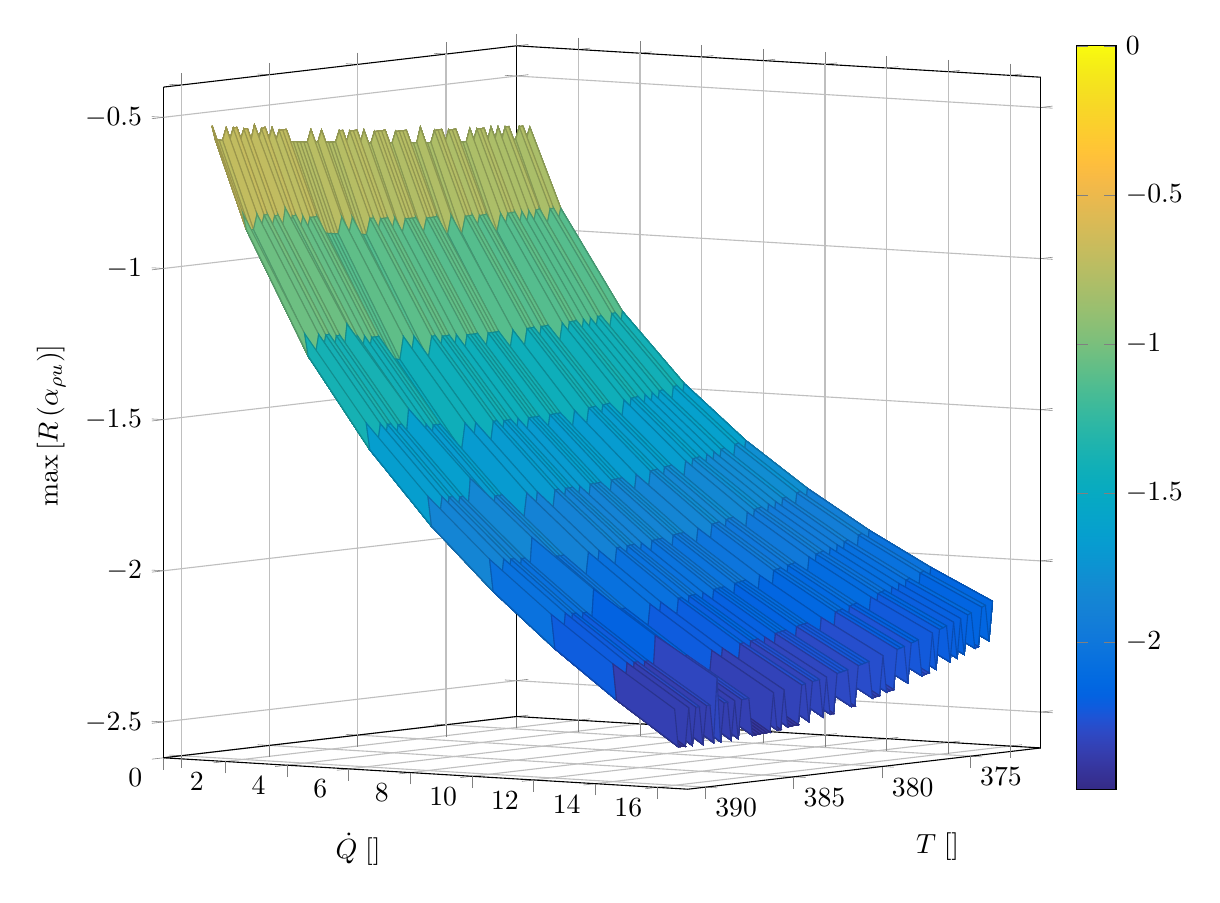
\begin{tikzpicture}

\begin{axis}[%
width=4.387in,
height=3.717in,
at={(0in,0in)},
scale only axis,
plot box ratio=1 1.063 1.109,
point meta min=-2.49392017330343,
point meta max=0,
xmin=371,
xmax=391,
tick align=outside,
xlabel={$T\;[\si{\kelvin}]$},
xmajorgrids,
ymin=0,
ymax=17,
ylabel={$\dot{Q}\;[\si{\kW}]$},
ymajorgrids,
zmin=-2.6186161819686,
zmax=-0.4,
zlabel={$\max\left[\mathbb{R}\left(\alpha_{\rho u}\right)\right]$},
zmajorgrids,
view={125.6}{4.79999999999997},
axis background/.style={fill=white},
colormap={mymap}{[1pt] rgb(0pt)=(0.2081,0.1663,0.5292); rgb(1pt)=(0.211624,0.189781,0.577676); rgb(2pt)=(0.212252,0.213771,0.626971); rgb(3pt)=(0.2081,0.2386,0.677086); rgb(4pt)=(0.195905,0.264457,0.7279); rgb(5pt)=(0.170729,0.291938,0.779248); rgb(6pt)=(0.125271,0.324243,0.830271); rgb(7pt)=(0.0591333,0.359833,0.868333); rgb(8pt)=(0.0116952,0.38751,0.881957); rgb(9pt)=(0.00595714,0.408614,0.882843); rgb(10pt)=(0.0165143,0.4266,0.878633); rgb(11pt)=(0.0328524,0.443043,0.871957); rgb(12pt)=(0.0498143,0.458571,0.864057); rgb(13pt)=(0.0629333,0.47369,0.855438); rgb(14pt)=(0.0722667,0.488667,0.8467); rgb(15pt)=(0.0779429,0.503986,0.838371); rgb(16pt)=(0.0793476,0.520024,0.831181); rgb(17pt)=(0.0749429,0.537543,0.826271); rgb(18pt)=(0.0640571,0.556986,0.823957); rgb(19pt)=(0.0487714,0.577224,0.822829); rgb(20pt)=(0.0343429,0.596581,0.819852); rgb(21pt)=(0.0265,0.6137,0.8135); rgb(22pt)=(0.0238905,0.628662,0.803762); rgb(23pt)=(0.0230905,0.641786,0.791267); rgb(24pt)=(0.0227714,0.653486,0.776757); rgb(25pt)=(0.0266619,0.664195,0.760719); rgb(26pt)=(0.0383714,0.674271,0.743552); rgb(27pt)=(0.0589714,0.683757,0.725386); rgb(28pt)=(0.0843,0.692833,0.706167); rgb(29pt)=(0.113295,0.7015,0.685857); rgb(30pt)=(0.145271,0.709757,0.664629); rgb(31pt)=(0.180133,0.717657,0.642433); rgb(32pt)=(0.217829,0.725043,0.619262); rgb(33pt)=(0.258643,0.731714,0.595429); rgb(34pt)=(0.302171,0.737605,0.571186); rgb(35pt)=(0.348167,0.742433,0.547267); rgb(36pt)=(0.395257,0.7459,0.524443); rgb(37pt)=(0.44201,0.748081,0.503314); rgb(38pt)=(0.487124,0.749062,0.483976); rgb(39pt)=(0.530029,0.749114,0.466114); rgb(40pt)=(0.570857,0.748519,0.44939); rgb(41pt)=(0.609852,0.747314,0.433686); rgb(42pt)=(0.6473,0.7456,0.4188); rgb(43pt)=(0.683419,0.743476,0.404433); rgb(44pt)=(0.71841,0.741133,0.390476); rgb(45pt)=(0.752486,0.7384,0.376814); rgb(46pt)=(0.785843,0.735567,0.363271); rgb(47pt)=(0.818505,0.732733,0.34979); rgb(48pt)=(0.850657,0.7299,0.336029); rgb(49pt)=(0.882433,0.727433,0.3217); rgb(50pt)=(0.913933,0.725786,0.306276); rgb(51pt)=(0.944957,0.726114,0.288643); rgb(52pt)=(0.973895,0.731395,0.266648); rgb(53pt)=(0.993771,0.745457,0.240348); rgb(54pt)=(0.999043,0.765314,0.216414); rgb(55pt)=(0.995533,0.786057,0.196652); rgb(56pt)=(0.988,0.8066,0.179367); rgb(57pt)=(0.978857,0.827143,0.163314); rgb(58pt)=(0.9697,0.848138,0.147452); rgb(59pt)=(0.962586,0.870514,0.1309); rgb(60pt)=(0.958871,0.8949,0.113243); rgb(61pt)=(0.959824,0.921833,0.0948381); rgb(62pt)=(0.9661,0.951443,0.0755333); rgb(63pt)=(0.9763,0.9831,0.0538)},
colorbar
]

\addplot3[%
surf,
shader=faceted,z buffer=sort,colormap={mymap}{[1pt] rgb(0pt)=(0.2081,0.1663,0.5292); rgb(1pt)=(0.211624,0.189781,0.577676); rgb(2pt)=(0.212252,0.213771,0.626971); rgb(3pt)=(0.2081,0.2386,0.677086); rgb(4pt)=(0.195905,0.264457,0.7279); rgb(5pt)=(0.170729,0.291938,0.779248); rgb(6pt)=(0.125271,0.324243,0.830271); rgb(7pt)=(0.0591333,0.359833,0.868333); rgb(8pt)=(0.0116952,0.38751,0.881957); rgb(9pt)=(0.00595714,0.408614,0.882843); rgb(10pt)=(0.0165143,0.4266,0.878633); rgb(11pt)=(0.0328524,0.443043,0.871957); rgb(12pt)=(0.0498143,0.458571,0.864057); rgb(13pt)=(0.0629333,0.47369,0.855438); rgb(14pt)=(0.0722667,0.488667,0.8467); rgb(15pt)=(0.0779429,0.503986,0.838371); rgb(16pt)=(0.0793476,0.520024,0.831181); rgb(17pt)=(0.0749429,0.537543,0.826271); rgb(18pt)=(0.0640571,0.556986,0.823957); rgb(19pt)=(0.0487714,0.577224,0.822829); rgb(20pt)=(0.0343429,0.596581,0.819852); rgb(21pt)=(0.0265,0.6137,0.8135); rgb(22pt)=(0.0238905,0.628662,0.803762); rgb(23pt)=(0.0230905,0.641786,0.791267); rgb(24pt)=(0.0227714,0.653486,0.776757); rgb(25pt)=(0.0266619,0.664195,0.760719); rgb(26pt)=(0.0383714,0.674271,0.743552); rgb(27pt)=(0.0589714,0.683757,0.725386); rgb(28pt)=(0.0843,0.692833,0.706167); rgb(29pt)=(0.113295,0.7015,0.685857); rgb(30pt)=(0.145271,0.709757,0.664629); rgb(31pt)=(0.180133,0.717657,0.642433); rgb(32pt)=(0.217829,0.725043,0.619262); rgb(33pt)=(0.258643,0.731714,0.595429); rgb(34pt)=(0.302171,0.737605,0.571186); rgb(35pt)=(0.348167,0.742433,0.547267); rgb(36pt)=(0.395257,0.7459,0.524443); rgb(37pt)=(0.44201,0.748081,0.503314); rgb(38pt)=(0.487124,0.749062,0.483976); rgb(39pt)=(0.530029,0.749114,0.466114); rgb(40pt)=(0.570857,0.748519,0.44939); rgb(41pt)=(0.609852,0.747314,0.433686); rgb(42pt)=(0.6473,0.7456,0.4188); rgb(43pt)=(0.683419,0.743476,0.404433); rgb(44pt)=(0.71841,0.741133,0.390476); rgb(45pt)=(0.752486,0.7384,0.376814); rgb(46pt)=(0.785843,0.735567,0.363271); rgb(47pt)=(0.818505,0.732733,0.34979); rgb(48pt)=(0.850657,0.7299,0.336029); rgb(49pt)=(0.882433,0.727433,0.3217); rgb(50pt)=(0.913933,0.725786,0.306276); rgb(51pt)=(0.944957,0.726114,0.288643); rgb(52pt)=(0.973895,0.731395,0.266648); rgb(53pt)=(0.993771,0.745457,0.240348); rgb(54pt)=(0.999043,0.765314,0.216414); rgb(55pt)=(0.995533,0.786057,0.196652); rgb(56pt)=(0.988,0.8066,0.179367); rgb(57pt)=(0.978857,0.827143,0.163314); rgb(58pt)=(0.9697,0.848138,0.147452); rgb(59pt)=(0.962586,0.870514,0.1309); rgb(60pt)=(0.958871,0.8949,0.113243); rgb(61pt)=(0.959824,0.921833,0.0948381); rgb(62pt)=(0.9661,0.951443,0.0755333); rgb(63pt)=(0.9763,0.9831,0.0538)},mesh/rows=91]
table[row sep=crcr, point meta=\thisrow{c}] {%
%
x	y	z	c\\
372	1	-0.65714133487345	-0.65714133487345\\
372	2	-0.918697726667254	-0.918697726667254\\
372	4	-1.24717732648168	-1.24717732648168\\
372	6	-1.47325602280098	-1.47325602280098\\
372	8	-1.64995965251814	-1.64995965251814\\
372	10	-1.79631584475912	-1.79631584475912\\
372	12	-1.92242742028045	-1.92242742028045\\
372	14	-2.03327974069231	-2.03327974069231\\
372	16	-2.13296037301046	-2.13296037301046\\
372.2	1	-0.694482970637787	-0.694482970637787\\
372.2	2	-0.974450799221156	-0.974450799221156\\
372.2	4	-1.32630467372264	-1.32630467372264\\
372.2	6	-1.56708451021139	-1.56708451021139\\
372.2	8	-1.75430071602811	-1.75430071602811\\
372.2	10	-1.90831029463281	-1.90831029463281\\
372.2	12	-2.04116499168891	-2.04116499168891\\
372.2	14	-2.15755512435571	-2.15755512435571\\
372.2	16	-2.26170758153982	-2.26170758153982\\
372.4	1	-0.650332514453688	-0.650332514453688\\
372.4	2	-0.915535693132852	-0.915535693132852\\
372.4	4	-1.24907277907881	-1.24907277907881\\
372.4	6	-1.47811580012182	-1.47811580012182\\
372.4	8	-1.6558300230356	-1.6558300230356\\
372.4	10	-1.80366309263328	-1.80366309263328\\
372.4	12	-1.93071276757186	-1.93071276757186\\
372.4	14	-2.04262277624899	-2.04262277624899\\
372.4	16	-2.14333678312979	-2.14333678312979\\
372.6	1	-0.650919533167014	-0.650919533167014\\
372.6	2	-0.916109999667646	-0.916109999667646\\
372.6	4	-1.25008348558844	-1.25008348558844\\
372.6	6	-1.47985841724464	-1.47985841724464\\
372.6	8	-1.65881417341363	-1.65881417341363\\
372.6	10	-1.80711179180743	-1.80711179180743\\
372.6	12	-1.93469486316662	-1.93469486316662\\
372.6	14	-2.04734866064323	-2.04734866064323\\
372.6	16	-2.14851869844781	-2.14851869844781\\
372.8	1	-0.69098426680428	-0.69098426680428\\
372.8	2	-0.974575826888542	-0.974575826888542\\
372.8	4	-1.32997931272475	-1.32997931272475\\
372.8	6	-1.57375169282693	-1.57375169282693\\
372.8	8	-1.76327868284757	-1.76327868284757\\
372.8	10	-1.91963301428046	-1.91963301428046\\
372.8	12	-2.0538707361812	-2.0538707361812\\
372.8	14	-2.17190899074737	-2.17190899074737\\
372.8	16	-2.27717496785219	-2.27717496785219\\
373	1	-0.690218944736538	-0.690218944736538\\
373	2	-0.97385488127032	-0.97385488127032\\
373	4	-1.32994956632427	-1.32994956632427\\
373	6	-1.57418880001696	-1.57418880001696\\
373	8	-1.76412064387971	-1.76412064387971\\
373	10	-1.92169275682746	-1.92169275682746\\
373	12	-2.05567750716958	-2.05567750716958\\
373	14	-2.17524303563164	-2.17524303563164\\
373	16	-2.2808276681989	-2.2808276681989\\
373.2	1	-0.646159181049745	-0.646159181049745\\
373.2	2	-0.911848226512781	-0.911848226512781\\
373.2	4	-1.25349098607577	-1.25349098607577\\
373.2	6	-1.48644292625941	-1.48644292625941\\
373.2	8	-1.6671337607679	-1.6671337607679\\
373.2	10	-1.81746025048005	-1.81746025048005\\
373.2	12	-1.94676841845306	-1.94676841845306\\
373.2	14	-2.06093556874148	-2.06093556874148\\
373.2	16	-2.16306831146047	-2.16306831146047\\
373.4	1	-0.647117616022668	-0.647117616022668\\
373.4	2	-0.915380497697963	-0.915380497697963\\
373.4	4	-1.25471259713582	-1.25471259713582\\
373.4	6	-1.48815199376845	-1.48815199376845\\
373.4	8	-1.66988054210761	-1.66988054210761\\
373.4	10	-1.81939794817142	-1.81939794817142\\
373.4	12	-1.95100890949592	-1.95100890949592\\
373.4	14	-2.06566506493477	-2.06566506493477\\
373.4	16	-2.16849153867223	-2.16849153867223\\
373.6	1	-0.689043171710939	-0.689043171710939\\
373.6	2	-0.973339718828795	-0.973339718828795\\
373.6	4	-1.33426684927607	-1.33426684927607\\
373.6	6	-1.58191694302912	-1.58191694302912\\
373.6	8	-1.77450329193387	-1.77450329193387\\
373.6	10	-1.93322165208086	-1.93322165208086\\
373.6	12	-2.07029033629305	-2.07029033629305\\
373.6	14	-2.1898582868659	-2.1898582868659\\
373.6	16	-2.29775880490821	-2.29775880490821\\
373.8	1	-0.643644900880525	-0.643644900880525\\
373.8	2	-0.915108952853627	-0.915108952853627\\
373.8	4	-1.25718355921556	-1.25718355921556\\
373.8	6	-1.49167975269388	-1.49167975269388\\
373.8	8	-1.67516583477519	-1.67516583477519\\
373.8	10	-1.82747520632472	-1.82747520632472\\
373.8	12	-1.95846540290198	-1.95846540290198\\
373.8	14	-2.07412915933375	-2.07412915933375\\
373.8	16	-2.17780391445869	-2.17780391445869\\
374	1	-0.687874586278309	-0.687874586278309\\
374	2	-0.974819140443089	-0.974819140443089\\
374	4	-1.33557717284793	-1.33557717284793\\
374	6	-1.58523942477441	-1.58523942477441\\
374	8	-1.77982542383676	-1.77982542383676\\
374	10	-1.93978857732646	-1.93978857732646\\
374	12	-2.07796273908462	-2.07796273908462\\
374	14	-2.1995505670544	-2.1995505670544\\
374	16	-2.30736964476723	-2.30736964476723\\
374.2	1	-0.641350166829656	-0.641350166829656\\
374.2	2	-0.914000464185237	-0.914000464185237\\
374.2	4	-1.25846732938178	-1.25846732938178\\
374.2	6	-1.49527063858998	-1.49527063858998\\
374.2	8	-1.68014048294186	-1.68014048294186\\
374.2	10	-1.83354039179698	-1.83354039179698\\
374.2	12	-1.9655932100163	-1.9655932100163\\
374.2	14	-2.08299746068605	-2.08299746068605\\
374.2	16	-2.18705996528623	-2.18705996528623\\
374.4	1	-0.686112406342787	-0.686112406342787\\
374.4	2	-0.972549005494837	-0.972549005494837\\
374.4	4	-1.33734728003342	-1.33734728003342\\
374.4	6	-1.58898331356315	-1.58898331356315\\
374.4	8	-1.78491037289216	-1.78491037289216\\
374.4	10	-1.94645023975405	-1.94645023975405\\
374.4	12	-2.08570631842347	-2.08570631842347\\
374.4	14	-2.20791163921819	-2.20791163921819\\
374.4	16	-2.31679166781754	-2.31679166781754\\
374.6	1	-0.642159337495892	-0.642159337495892\\
374.6	2	-0.912689080882333	-0.912689080882333\\
374.6	4	-1.26007917230306	-1.26007917230306\\
374.6	6	-1.49891897336801	-1.49891897336801\\
374.6	8	-1.685556805338	-1.685556805338\\
374.6	10	-1.83997188272396	-1.83997188272396\\
374.6	12	-1.97338559254218	-1.97338559254218\\
374.6	14	-2.09099822374298	-2.09099822374298\\
374.6	16	-2.1965222036853	-2.1965222036853\\
374.8	1	-0.642452109424468	-0.642452109424468\\
374.8	2	-0.913710870172404	-0.913710870172404\\
374.8	4	-1.26077649719152	-1.26077649719152\\
374.8	6	-1.50069889010129	-1.50069889010129\\
374.8	8	-1.68769374294889	-1.68769374294889\\
374.8	10	-1.84302151662544	-1.84302151662544\\
374.8	12	-1.97736292715453	-1.97736292715453\\
374.8	14	-2.09522728698286	-2.09522728698286\\
374.8	16	-2.20132288622915	-2.20132288622915\\
375	1	-0.642604674321815	-0.642604674321815\\
375	2	-0.914326984886252	-0.914326984886252\\
375	4	-1.26140968316531	-1.26140968316531\\
375	6	-1.50201644174737	-1.50201644174737\\
375	8	-1.68997415893948	-1.68997415893948\\
375	10	-1.84608184907419	-1.84608184907419\\
375	12	-1.98066522223879	-1.98066522223879\\
375	14	-2.09948401211843	-2.09948401211843\\
375	16	-2.20571335808085	-2.20571335808085\\
375.2	1	-0.681667432397533	-0.681667432397533\\
375.2	2	-0.97074322259142	-0.97074322259142\\
375.2	4	-1.34053700757818	-1.34053700757818\\
375.2	6	-1.59557341378579	-1.59557341378579\\
375.2	8	-1.79432944891061	-1.79432944891061\\
375.2	10	-1.95856563034898	-1.95856563034898\\
375.2	12	-2.10006341803196	-2.10006341803196\\
375.2	14	-2.22458299491725	-2.22458299491725\\
375.2	16	-2.33579114048213	-2.33579114048213\\
375.4	1	-0.638081844568953	-0.638081844568953\\
375.4	2	-0.912423415087328	-0.912423415087328\\
375.4	4	-1.26267339691163	-1.26267339691163\\
375.4	6	-1.50502652601497	-1.50502652601497\\
375.4	8	-1.69433499348903	-1.69433499348903\\
375.4	10	-1.85188879602387	-1.85188879602387\\
375.4	12	-1.98768707178609	-1.98768707178609\\
375.4	14	-2.10746168353287	-2.10746168353287\\
375.4	16	-2.21463770819601	-2.21463770819601\\
375.6	1	-0.680336531314139	-0.680336531314139\\
375.6	2	-0.969536876001351	-0.969536876001351\\
375.6	4	-1.34127672764116	-1.34127672764116\\
375.6	6	-1.59853605324212	-1.59853605324212\\
375.6	8	-1.79866269177861	-1.79866269177861\\
375.6	10	-1.96483118466741	-1.96483118466741\\
375.6	12	-2.10729277397882	-2.10729277397882\\
375.6	14	-2.232385064177	-2.232385064177\\
375.6	16	-2.34499838423011	-2.34499838423011\\
375.8	1	-0.679348570373607	-0.679348570373607\\
375.8	2	-0.96872196758092	-0.96872196758092\\
375.8	4	-1.34104224033468	-1.34104224033468\\
375.8	6	-1.59855642835847	-1.59855642835847\\
375.8	8	-1.79929220807725	-1.79929220807725\\
375.8	10	-1.96579788101191	-1.96579788101191\\
375.8	12	-2.10873256495103	-2.10873256495103\\
375.8	14	-2.23461415835048	-2.23461415835048\\
375.8	16	-2.34762862680246	-2.34762862680246\\
376	1	-0.678273796203901	-0.678273796203901\\
376	2	-0.96828898069716	-0.96828898069716\\
376	4	-1.3410002907329	-1.3410002907329\\
376	6	-1.59922895183184	-1.59922895183184\\
376	8	-1.80080917474845	-1.80080917474845\\
376	10	-1.96824518925096	-1.96824518925096\\
376	12	-2.11215876099007	-2.11215876099007\\
376	14	-2.23911746562444	-2.23911746562444\\
376	16	-2.35174281858139	-2.35174281858139\\
376.2	1	-0.634090489195138	-0.634090489195138\\
376.2	2	-0.909742976753364	-0.909742976753364\\
376.2	4	-1.2647360429191	-1.2647360429191\\
376.2	6	-1.51046941858947	-1.51046941858947\\
376.2	8	-1.70270103687642	-1.70270103687642\\
376.2	10	-1.86268062906305	-1.86268062906305\\
376.2	12	-2.00062605513612	-2.00062605513612\\
376.2	14	-2.1221876309388	-2.1221876309388\\
376.2	16	-2.23164191548546	-2.23164191548546\\
376.4	1	-0.634790412043854	-0.634790412043854\\
376.4	2	-0.910413609327056	-0.910413609327056\\
376.4	4	-1.26538700696011	-1.26538700696011\\
376.4	6	-1.51158931515124	-1.51158931515124\\
376.4	8	-1.70490815999055	-1.70490815999055\\
376.4	10	-1.86528092551309	-1.86528092551309\\
376.4	12	-2.00393726152159	-2.00393726152159\\
376.4	14	-2.1261111499183	-2.1261111499183\\
376.4	16	-2.23569423148245	-2.23569423148245\\
376.6	1	-0.634954883394281	-0.634954883394281\\
376.6	2	-0.910781965327706	-0.910781965327706\\
376.6	4	-1.26579166504579	-1.26579166504579\\
376.6	6	-1.5129133219079	-1.5129133219079\\
376.6	8	-1.706315446574	-1.706315446574\\
376.6	10	-1.86803258530339	-1.86803258530339\\
376.6	12	-2.00702813103644	-2.00702813103644\\
376.6	14	-2.12985269437381	-2.12985269437381\\
376.6	16	-2.23970358144941	-2.23970358144941\\
376.8	1	-0.674033420250061	-0.674033420250061\\
376.8	2	-0.965860021201036	-0.965860021201036\\
376.8	4	-1.34379832586774	-1.34379832586774\\
376.8	6	-1.60605897931779	-1.60605897931779\\
376.8	8	-1.81106499102593	-1.81106499102593\\
376.8	10	-1.9808696774995	-1.9808696774995\\
376.8	12	-2.12699744868046	-2.12699744868046\\
376.8	14	-2.2550501828103	-2.2550501828103\\
376.8	16	-2.37005200209202	-2.37005200209202\\
377	1	-0.629630526577255	-0.629630526577255\\
377	2	-0.906611566324576	-0.906611566324576\\
377	4	-1.26584743908569	-1.26584743908569\\
377	6	-1.51527930509331	-1.51527930509331\\
377	8	-1.71052941873879	-1.71052941873879\\
377	10	-1.87299737101979	-1.87299737101979\\
377	12	-2.01179820348736	-2.01179820348736\\
377	14	-2.13697480441338	-2.13697480441338\\
377	16	-2.24787585201142	-2.24787585201142\\
377.2	1	-0.630265676787372	-0.630265676787372\\
377.2	2	-0.907625686492712	-0.907625686492712\\
377.2	4	-1.26638577632454	-1.26638577632454\\
377.2	6	-1.51608080338275	-1.51608080338275\\
377.2	8	-1.71247825617154	-1.71247825617154\\
377.2	10	-1.87536504858751	-1.87536504858751\\
377.2	12	-2.01574373554954	-2.01574373554954\\
377.2	14	-2.14003947465388	-2.14003947465388\\
377.2	16	-2.25162693312207	-2.25162693312207\\
377.4	1	-0.63048036858626	-0.63048036858626\\
377.4	2	-0.907876553568176	-0.907876553568176\\
377.4	4	-1.26691572219853	-1.26691572219853\\
377.4	6	-1.51696820101001	-1.51696820101001\\
377.4	8	-1.71371876422806	-1.71371876422806\\
377.4	10	-1.87774748224758	-1.87774748224758\\
377.4	12	-2.01861237628873	-2.01861237628873\\
377.4	14	-2.14332895945996	-2.14332895945996\\
377.4	16	-2.25545603185738	-2.25545603185738\\
377.6	1	-0.669098324336016	-0.669098324336016\\
377.6	2	-0.963222660140331	-0.963222660140331\\
377.6	4	-1.34446069273673	-1.34446069273673\\
377.6	6	-1.6103251039375	-1.6103251039375\\
377.6	8	-1.81779666713223	-1.81779666713223\\
377.6	10	-1.9902305779633	-1.9902305779633\\
377.6	12	-2.13871324477276	-2.13871324477276\\
377.6	14	-2.26938057167787	-2.26938057167787\\
377.6	16	-2.38634793728217	-2.38634793728217\\
377.8	1	-0.667729751033848	-0.667729751033848\\
377.8	2	-0.961892880085077	-0.961892880085077\\
377.8	4	-1.34391736364235	-1.34391736364235\\
377.8	6	-1.61001353157462	-1.61001353157462\\
377.8	8	-1.81795848519812	-1.81795848519812\\
377.8	10	-1.99063640075915	-1.99063640075915\\
377.8	12	-2.13954489264104	-2.13954489264104\\
377.8	14	-2.27064702714753	-2.27064702714753\\
377.8	16	-2.3885046018305	-2.3885046018305\\
378	1	-0.666901582176485	-0.666901582176485\\
378	2	-0.961179280799425	-0.961179280799425\\
378	4	-1.34352139308565	-1.34352139308565\\
378	6	-1.61000544799551	-1.61000544799551\\
378	8	-1.8185884136962	-1.8185884136962\\
378	10	-1.99257169658795	-1.99257169658795\\
378	12	-2.14183109342979	-2.14183109342979\\
378	14	-2.27359220759497	-2.27359220759497\\
378	16	-2.39180964540266	-2.39180964540266\\
378.2	1	-0.614740877636884	-0.614740877636884\\
378.2	2	-0.900433033976331	-0.900433033976331\\
378.2	4	-1.2664274694105	-1.2664274694105\\
378.2	6	-1.52052916482237	-1.52052916482237\\
378.2	8	-1.7200072178784	-1.7200072178784\\
378.2	10	-1.8857150497438	-1.8857150497438\\
378.2	12	-2.02882017554459	-2.02882017554459\\
378.2	14	-2.15634304489669	-2.15634304489669\\
378.2	16	-2.2703207059882	-2.2703207059882\\
378.4	1	-0.664040574193704	-0.664040574193704\\
378.4	2	-0.958702510366147	-0.958702510366147\\
378.4	4	-1.34406624492326	-1.34406624492326\\
378.4	6	-1.61314579786836	-1.61314579786836\\
378.4	8	-1.82406602932273	-1.82406602932273\\
378.4	10	-1.99891885320838	-1.99891885320838\\
378.4	12	-2.14971617942088	-2.14971617942088\\
378.4	14	-2.28232115357663	-2.28232115357663\\
378.4	16	-2.40112080171599	-2.40112080171599\\
378.6	1	-0.662571512327148	-0.662571512327148\\
378.6	2	-0.957916076058367	-0.957916076058367\\
378.6	4	-1.34328394799238	-1.34328394799238\\
378.6	6	-1.6129276816431	-1.6129276816431\\
378.6	8	-1.82407279685909	-1.82407279685909\\
378.6	10	-1.999344097341	-1.999344097341\\
378.6	12	-2.15033905858301	-2.15033905858301\\
378.6	14	-2.28347642238259	-2.28347642238259\\
378.6	16	-2.40266521725277	-2.40266521725277\\
378.8	1	-0.661616946739246	-0.661616946739246\\
378.8	2	-0.95681010094913	-0.95681010094913\\
378.8	4	-1.34281683085002	-1.34281683085002\\
378.8	6	-1.61291303472869	-1.61291303472869\\
378.8	8	-1.82459655976869	-1.82459655976869\\
378.8	10	-2.00055303416387	-2.00055303416387\\
378.8	12	-2.15279778280446	-2.15279778280446\\
378.8	14	-2.28643164177401	-2.28643164177401\\
378.8	16	-2.40623266642322	-2.40623266642322\\
379	1	-0.618804365231425	-0.618804365231425\\
379	2	-0.897530050891944	-0.897530050891944\\
379	4	-1.26619659345656	-1.26619659345656\\
379	6	-1.52318653463476	-1.52318653463476\\
379	8	-1.72552474177849	-1.72552474177849\\
379	10	-1.89436717818216	-1.89436717818216\\
379	12	-2.03925813434605	-2.03925813434605\\
379	14	-2.16892818539482	-2.16892818539482\\
379	16	-2.28413468740807	-2.28413468740807\\
379.2	1	-0.619129293928785	-0.619129293928785\\
379.2	2	-0.898261689412719	-0.898261689412719\\
379.2	4	-1.26639976527846	-1.26639976527846\\
379.2	6	-1.52378734135372	-1.52378734135372\\
379.2	8	-1.72667332993971	-1.72667332993971\\
379.2	10	-1.89590982135508	-1.89590982135508\\
379.2	12	-2.04237535070366	-2.04237535070366\\
379.2	14	-2.1711761296575	-2.1711761296575\\
379.2	16	-2.28730590463889	-2.28730590463889\\
379.4	1	-0.61913461800317	-0.61913461800317\\
379.4	2	-0.898733107709826	-0.898733107709826\\
379.4	4	-1.26670871172033	-1.26670871172033\\
379.4	6	-1.52435797721468	-1.52435797721468\\
379.4	8	-1.72748912485362	-1.72748912485362\\
379.4	10	-1.89693055006879	-1.89693055006879\\
379.4	12	-2.0441627221264	-2.0441627221264\\
379.4	14	-2.17344628865405	-2.17344628865405\\
379.4	16	-2.29093054998734	-2.29093054998734\\
379.6	1	-0.618847293625989	-0.618847293625989\\
379.6	2	-0.898695787354079	-0.898695787354079\\
379.6	4	-1.26678182953248	-1.26678182953248\\
379.6	6	-1.52499489970877	-1.52499489970877\\
379.6	8	-1.72946561592842	-1.72946561592842\\
379.6	10	-1.89932431739915	-1.89932431739915\\
379.6	12	-2.0467348328515	-2.0467348328515\\
379.6	14	-2.17735668836816	-2.17735668836816\\
379.6	16	-2.29377286895156	-2.29377286895156\\
379.8	1	-0.655275340402921	-0.655275340402921\\
379.8	2	-0.951902443548959	-0.951902443548959\\
379.8	4	-1.34193787122488	-1.34193787122488\\
379.8	6	-1.61611402020919	-1.61611402020919\\
379.8	8	-1.83241699102336	-1.83241699102336\\
379.8	10	-2.01185718654677	-2.01185718654677\\
379.8	12	-2.16645692254457	-2.16645692254457\\
379.8	14	-2.3027486976912	-2.3027486976912\\
379.8	16	-2.42561668391053	-2.42561668391053\\
380	1	-0.654100641334998	-0.654100641334998\\
380	2	-0.950985837230508	-0.950985837230508\\
380	4	-1.3411966935945	-1.3411966935945\\
380	6	-1.61583193657843	-1.61583193657843\\
380	8	-1.8322306809938	-1.8322306809938\\
380	10	-2.01200815345415	-2.01200815345415\\
380	12	-2.16688929087772	-2.16688929087772\\
380	14	-2.30344240196891	-2.30344240196891\\
380	16	-2.42603849995027	-2.42603849995027\\
380.2	1	-0.610290944389434	-0.610290944389434\\
380.2	2	-0.893246429097688	-0.893246429097688\\
380.2	4	-1.26421077547758	-1.26421077547758\\
380.2	6	-1.52583732456555	-1.52583732456555\\
380.2	8	-1.73227002837704	-1.73227002837704\\
380.2	10	-1.90472346869291	-1.90472346869291\\
380.2	12	-2.05339881263478	-2.05339881263478\\
380.2	14	-2.18496701620829	-2.18496701620829\\
380.2	16	-2.30318859206456	-2.30318859206456\\
380.4	1	-0.611015764852675	-0.611015764852675\\
380.4	2	-0.893436709435529	-0.893436709435529\\
380.4	4	-1.26447949453986	-1.26447949453986\\
380.4	6	-1.52628308756168	-1.52628308756168\\
380.4	8	-1.73311998474986	-1.73311998474986\\
380.4	10	-1.90567477962398	-1.90567477962398\\
380.4	12	-2.05462208498451	-2.05462208498451\\
380.4	14	-2.18658032917172	-2.18658032917172\\
380.4	16	-2.30602254206388	-2.30602254206388\\
380.6	1	-0.611185502003486	-0.611185502003486\\
380.6	2	-0.893256578558734	-0.893256578558734\\
380.6	4	-1.26457389626258	-1.26457389626258\\
380.6	6	-1.52667161111841	-1.52667161111841\\
380.6	8	-1.73373210061237	-1.73373210061237\\
380.6	10	-1.90695396591993	-1.90695396591993\\
380.6	12	-2.05630694179691	-2.05630694179691\\
380.6	14	-2.18934658237462	-2.18934658237462\\
380.6	16	-2.30891821476897	-2.30891821476897\\
380.8	1	-0.611000770463829	-0.611000770463829\\
380.8	2	-0.892903759733363	-0.892903759733363\\
380.8	4	-1.26449439568407	-1.26449439568407\\
380.8	6	-1.52697964667346	-1.52697964667346\\
380.8	8	-1.73471168701065	-1.73471168701065\\
380.8	10	-1.90858609500112	-1.90858609500112\\
380.8	12	-2.0587288953277	-2.0587288953277\\
380.8	14	-2.19175302678017	-2.19175302678017\\
380.8	16	-2.31152779658419	-2.31152779658419\\
381	1	-0.648060806680189	-0.648060806680189\\
381	2	-0.944193781033525	-0.944193781033525\\
381	4	-1.33960871731018	-1.33960871731018\\
381	6	-1.61808527210476	-1.61808527210476\\
381	8	-1.83695424523719	-1.83695424523719\\
381	10	-2.0203431863635	-2.0203431863635\\
381	12	-2.17779379237774	-2.17779379237774\\
381	14	-2.3170071200309	-2.3170071200309\\
381	16	-2.44213385364039	-2.44213385364039\\
381.2	1	-0.646023241576395	-0.646023241576395\\
381.2	2	-0.943104069854508	-0.943104069854508\\
381.2	4	-1.33770683967372	-1.33770683967372\\
381.2	6	-1.61735133927237	-1.61735133927237\\
381.2	8	-1.83688422078828	-1.83688422078828\\
381.2	10	-2.02030643669422	-2.02030643669422\\
381.2	12	-2.17819694724244	-2.17819694724244\\
381.2	14	-2.31777278423724	-2.31777278423724\\
381.2	16	-2.44282109037527	-2.44282109037527\\
381.4	1	-0.602098638502642	-0.602098638502642\\
381.4	2	-0.885049743458779	-0.885049743458779\\
381.4	4	-1.26031876543399	-1.26031876543399\\
381.4	6	-1.52513133293061	-1.52513133293061\\
381.4	8	-1.73648516875857	-1.73648516875857\\
381.4	10	-1.91234266737061	-1.91234266737061\\
381.4	12	-2.06434117928853	-2.06434117928853\\
381.4	14	-2.19919612535098	-2.19919612535098\\
381.4	16	-2.3195316842143	-2.3195316842143\\
381.6	1	-0.642812609290841	-0.642812609290841\\
381.6	2	-0.939979709764765	-0.939979709764765\\
381.6	4	-1.33604300887741	-1.33604300887741\\
381.6	6	-1.61717932392908	-1.61717932392908\\
381.6	8	-1.83891371321812	-1.83891371321812\\
381.6	10	-2.02355821249285	-2.02355821249285\\
381.6	12	-2.18310925259799	-2.18310925259799\\
381.6	14	-2.32389278410315	-2.32389278410315\\
381.6	16	-2.44997763806237	-2.44997763806237\\
381.8	1	-0.599231307607789	-0.599231307607789\\
381.8	2	-0.882828814191289	-0.882828814191289\\
381.8	4	-1.25913665388888	-1.25913665388888\\
381.8	6	-1.52595540417709	-1.52595540417709\\
381.8	8	-1.73767898813855	-1.73767898813855\\
381.8	10	-1.91444079200576	-1.91444079200576\\
381.8	12	-2.06761980692492	-2.06761980692492\\
381.8	14	-2.20267199289859	-2.20267199289859\\
381.8	16	-2.32482395571172	-2.32482395571172\\
382	1	-0.59998037575202	-0.59998037575202\\
382	2	-0.883049155406962	-0.883049155406962\\
382	4	-1.25937429297975	-1.25937429297975\\
382	6	-1.5266213237438	-1.5266213237438\\
382	8	-1.73824927308958	-1.73824927308958\\
382	10	-1.91521977398173	-1.91521977398173\\
382	12	-2.06867201167915	-2.06867201167915\\
382	14	-2.20478712440741	-2.20478712440741\\
382	16	-2.32684441025567	-2.32684441025567\\
382.2	1	-0.600146593050105	-0.600146593050105\\
382.2	2	-0.882920904529422	-0.882920904529422\\
382.2	4	-1.25935295874043	-1.25935295874043\\
382.2	6	-1.52692421855477	-1.52692421855477\\
382.2	8	-1.73872589766429	-1.73872589766429\\
382.2	10	-1.91634164489127	-1.91634164489127\\
382.2	12	-2.06993094586799	-2.06993094586799\\
382.2	14	-2.20691789726071	-2.20691789726071\\
382.2	16	-2.3286587810506	-2.3286587810506\\
382.4	1	-0.636084439611679	-0.636084439611679\\
382.4	2	-0.93462529991168	-0.93462529991168\\
382.4	4	-1.33254585160357	-1.33254585160357\\
382.4	6	-1.6157500321504	-1.6157500321504\\
382.4	8	-1.84031759832386	-1.84031759832386\\
382.4	10	-2.02742991902566	-2.02742991902566\\
382.4	12	-2.18900752195633	-2.18900752195633\\
382.4	14	-2.33150834733423	-2.33150834733423\\
382.4	16	-2.4594551195245	-2.4594551195245\\
382.6	1	-0.594692656714956	-0.594692656714956\\
382.6	2	-0.877919211915781	-0.877919211915781\\
382.6	4	-1.25542769791919	-1.25542769791919\\
382.6	6	-1.52443777952631	-1.52443777952631\\
382.6	8	-1.73881732780587	-1.73881732780587\\
382.6	10	-1.91788980516121	-1.91788980516121\\
382.6	12	-2.07299190714896	-2.07299190714896\\
382.6	14	-2.21009090559526	-2.21009090559526\\
382.6	16	-2.333386175013	-2.333386175013\\
382.8	1	-0.595056566038031	-0.595056566038031\\
382.8	2	-0.878076002556842	-0.878076002556842\\
382.8	4	-1.25567537885563	-1.25567537885563\\
382.8	6	-1.5249218908114	-1.5249218908114\\
382.8	8	-1.73950675065575	-1.73950675065575\\
382.8	10	-1.9186072135767	-1.9186072135767\\
382.8	12	-2.07391372461403	-2.07391372461403\\
382.8	14	-2.21181509332397	-2.21181509332397\\
382.8	16	-2.33629165513546	-2.33629165513546\\
383	1	-0.630729716056449	-0.630729716056449\\
383	2	-0.929779308432056	-0.929779308432056\\
383	4	-1.32944872414283	-1.32944872414283\\
383	6	-1.61479204140429	-1.61479204140429\\
383	8	-1.84090044686534	-1.84090044686534\\
383	10	-2.02929124915319	-2.02929124915319\\
383	12	-2.1925274849191	-2.1925274849191\\
383	14	-2.33644165457125	-2.33644165457125\\
383	16	-2.46553394643474	-2.46553394643474\\
383.2	1	-0.629530133758153	-0.629530133758153\\
383.2	2	-0.928697393486836	-0.928697393486836\\
383.2	4	-1.32815176978234	-1.32815176978234\\
383.2	6	-1.61369640025045	-1.61369640025045\\
383.2	8	-1.84028965955329	-1.84028965955329\\
383.2	10	-2.0290951854636	-2.0290951854636\\
383.2	12	-2.19243739096701	-2.19243739096701\\
383.2	14	-2.33658600538034	-2.33658600538034\\
383.2	16	-2.46602791155875	-2.46602791155875\\
383.4	1	-0.628655179378892	-0.628655179378892\\
383.4	2	-0.925596469267958	-0.925596469267958\\
383.4	4	-1.3273540382143	-1.3273540382143\\
383.4	6	-1.61305203512704	-1.61305203512704\\
383.4	8	-1.84002163510638	-1.84002163510638\\
383.4	10	-2.02908373368865	-2.02908373368865\\
383.4	12	-2.19271691995482	-2.19271691995482\\
383.4	14	-2.33742573553797	-2.33742573553797\\
383.4	16	-2.46711793264777	-2.46711793264777\\
383.6	1	-0.626700043235197	-0.626700043235197\\
383.6	2	-0.924588515684947	-0.924588515684947\\
383.6	4	-1.32638314646197	-1.32638314646197\\
383.6	6	-1.61257139100202	-1.61257139100202\\
383.6	8	-1.83952214554053	-1.83952214554053\\
383.6	10	-2.02919893257797	-2.02919893257797\\
383.6	12	-2.19321538469895	-2.19321538469895\\
383.6	14	-2.33835649584013	-2.33835649584013\\
383.6	16	-2.46885619641299	-2.46885619641299\\
383.8	1	-0.585879913882203	-0.585879913882203\\
383.8	2	-0.868046266922808	-0.868046266922808\\
383.8	4	-1.24903903019422	-1.24903903019422\\
383.8	6	-1.52216002180135	-1.52216002180135\\
383.8	8	-1.73929140831006	-1.73929140831006\\
383.8	10	-1.92145401353618	-1.92145401353618\\
383.8	12	-2.07928156506637	-2.07928156506637\\
383.8	14	-2.21937026437177	-2.21937026437177\\
383.8	16	-2.34539722686194	-2.34539722686194\\
384	1	-0.623465934405151	-0.623465934405151\\
384	2	-0.920673829202679	-0.920673829202679\\
384	4	-1.32358763516036	-1.32358763516036\\
384	6	-1.61151543375138	-1.61151543375138\\
384	8	-1.84032141791555	-1.84032141791555\\
384	10	-2.03184026049269	-2.03184026049269\\
384	12	-2.19694980699015	-2.19694980699015\\
384	14	-2.34349553317227	-2.34349553317227\\
384	16	-2.47479363403094	-2.47479363403094\\
384.2	1	-0.622559054436374	-0.622559054436374\\
384.2	2	-0.919512225582529	-0.919512225582529\\
384.2	4	-1.32226894940324	-1.32226894940324\\
384.2	6	-1.61039142435055	-1.61039142435055\\
384.2	8	-1.83973932749715	-1.83973932749715\\
384.2	10	-2.03116797534951	-2.03116797534951\\
384.2	12	-2.19691627949235	-2.19691627949235\\
384.2	14	-2.34340895971311	-2.34340895971311\\
384.2	16	-2.4749942946968	-2.4749942946968\\
384.4	1	-0.580360074087889	-0.580360074087889\\
384.4	2	-0.862659891828332	-0.862659891828332\\
384.4	4	-1.24591585383841	-1.24591585383841\\
384.4	6	-1.51995516895539	-1.51995516895539\\
384.4	8	-1.73875906403307	-1.73875906403307\\
384.4	10	-1.92264213797928	-1.92264213797928\\
384.4	12	-2.081992390493	-2.081992390493\\
384.4	14	-2.22307911001036	-2.22307911001036\\
384.4	16	-2.35048963564723	-2.35048963564723\\
384.6	1	-0.619993685199195	-0.619993685199195\\
384.6	2	-0.916616094310489	-0.916616094310489\\
384.6	4	-1.32031995446202	-1.32031995446202\\
384.6	6	-1.60871917891086	-1.60871917891086\\
384.6	8	-1.83952675639632	-1.83952675639632\\
384.6	10	-2.03233737687131	-2.03233737687131\\
384.6	12	-2.19923879065179	-2.19923879065179\\
384.6	14	-2.34688124742637	-2.34688124742637\\
384.6	16	-2.47962919800865	-2.47962919800865\\
384.8	1	-0.618527707549549	-0.618527707549549\\
384.8	2	-0.91498820125116	-0.91498820125116\\
384.8	4	-1.31792990065169	-1.31792990065169\\
384.8	6	-1.60759983485522	-1.60759983485522\\
384.8	8	-1.83841222966708	-1.83841222966708\\
384.8	10	-2.03187416069686	-2.03187416069686\\
384.8	12	-2.19914218923707	-2.19914218923707\\
384.8	14	-2.34669634869046	-2.34669634869046\\
384.8	16	-2.47963979621568	-2.47963979621568\\
385	1	-0.61697136211564	-0.61697136211564\\
385	2	-0.913008808367706	-0.913008808367706\\
385	4	-1.31658416812497	-1.31658416812497\\
385	6	-1.6068383953639	-1.6068383953639\\
385	8	-1.83758762945484	-1.83758762945484\\
385	10	-2.03153645483324	-2.03153645483324\\
385	12	-2.19908613495017	-2.19908613495017\\
385	14	-2.34687280561766	-2.34687280561766\\
385	16	-2.48018542922321	-2.48018542922321\\
385.2	1	-0.614883377914391	-0.614883377914391\\
385.2	2	-0.911062474348145	-0.911062474348145\\
385.2	4	-1.31435717903444	-1.31435717903444\\
385.2	6	-1.60599961404363	-1.60599961404363\\
385.2	8	-1.83706392912677	-1.83706392912677\\
385.2	10	-2.03133061544604	-2.03133061544604\\
385.2	12	-2.19906355895839	-2.19906355895839\\
385.2	14	-2.34740706599977	-2.34740706599977\\
385.2	16	-2.48096325828062	-2.48096325828062\\
385.4	1	-0.613556250277742	-0.613556250277742\\
385.4	2	-0.909324983991346	-0.909324983991346\\
385.4	4	-1.31332988919071	-1.31332988919071\\
385.4	6	-1.60492600919503	-1.60492600919503\\
385.4	8	-1.8365168217108	-1.8365168217108\\
385.4	10	-2.03107551881992	-2.03107551881992\\
385.4	12	-2.19926778572029	-2.19926778572029\\
385.4	14	-2.34820400846422	-2.34820400846422\\
385.4	16	-2.48223208263558	-2.48223208263558\\
385.6	1	-0.611773286117575	-0.611773286117575\\
385.6	2	-0.90776796766944	-0.90776796766944\\
385.6	4	-1.31196145621857	-1.31196145621857\\
385.6	6	-1.60381485883043	-1.60381485883043\\
385.6	8	-1.83591026691032	-1.83591026691032\\
385.6	10	-2.03082399395232	-2.03082399395232\\
385.6	12	-2.19952991283995	-2.19952991283995\\
385.6	14	-2.34874822956019	-2.34874822956019\\
385.6	16	-2.48316884900387	-2.48316884900387\\
385.8	1	-0.569446448714632	-0.569446448714632\\
385.8	2	-0.85121171218153	-0.85121171218153\\
385.8	4	-1.23584276179554	-1.23584276179554\\
385.8	6	-1.51381441534214	-1.51381441534214\\
385.8	8	-1.73600117121322	-1.73600117121322\\
385.8	10	-1.92244054266887	-1.92244054266887\\
385.8	12	-2.08556919346382	-2.08556919346382\\
385.8	14	-2.2297326830973	-2.2297326830973\\
385.8	16	-2.35948313999021	-2.35948313999021\\
386	1	-0.570108451477874	-0.570108451477874\\
386	2	-0.851573944154072	-0.851573944154072\\
386	4	-1.23593248748362	-1.23593248748362\\
386	6	-1.51398423555733	-1.51398423555733\\
386	8	-1.7362899952824	-1.7362899952824\\
386	10	-1.92327251847882	-1.92327251847882\\
386	12	-2.08596396076774	-2.08596396076774\\
386	14	-2.23059200575339	-2.23059200575339\\
386	16	-2.36065767775274	-2.36065767775274\\
386.2	1	-0.570362830969477	-0.570362830969477\\
386.2	2	-0.851459977501377	-0.851459977501377\\
386.2	4	-1.23555432128509	-1.23555432128509\\
386.2	6	-1.5137401518853	-1.5137401518853\\
386.2	8	-1.73625271974037	-1.73625271974037\\
386.2	10	-1.92346049377543	-1.92346049377543\\
386.2	12	-2.08630202161719	-2.08630202161719\\
386.2	14	-2.23115472754477	-2.23115472754477\\
386.2	16	-2.3614896073415	-2.3614896073415\\
386.4	1	-0.605383617617757	-0.605383617617757\\
386.4	2	-0.90044676925821	-0.90044676925821\\
386.4	4	-1.3052100243066	-1.3052100243066\\
386.4	6	-1.59871665344549	-1.59871665344549\\
386.4	8	-1.8334920109081	-1.8334920109081\\
386.4	10	-2.03062423450827	-2.03062423450827\\
386.4	12	-2.20184574839972	-2.20184574839972\\
386.4	14	-2.35325764808281	-2.35325764808281\\
386.4	16	-2.48870371656086	-2.48870371656086\\
386.6	1	-0.558876028937134	-0.558876028937134\\
386.6	2	-0.845347780583858	-0.845347780583858\\
386.6	4	-1.22938179397637	-1.22938179397637\\
386.6	6	-1.5090920786151	-1.5090920786151\\
386.6	8	-1.73297944635418	-1.73297944635418\\
386.6	10	-1.9220200990263	-1.9220200990263\\
386.6	12	-2.08627476867215	-2.08627476867215\\
386.6	14	-2.23196227472598	-2.23196227472598\\
386.6	16	-2.36222239616175	-2.36222239616175\\
386.8	1	-0.600982751029289	-0.600982751029289\\
386.8	2	-0.895800596620007	-0.895800596620007\\
386.8	4	-1.30176956696145	-1.30176956696145\\
386.8	6	-1.59602097018607	-1.59602097018607\\
386.8	8	-1.8316034084918	-1.8316034084918\\
386.8	10	-2.02957533412124	-2.02957533412124\\
386.8	12	-2.2014510824557	-2.2014510824557\\
386.8	14	-2.35382829727078	-2.35382829727078\\
386.8	16	-2.49097370261138	-2.49097370261138\\
387	1	-0.55433570062104	-0.55433570062104\\
387	2	-0.838859447869827	-0.838859447869827\\
387	4	-1.22625248006204	-1.22625248006204\\
387	6	-1.50627757123014	-1.50627757123014\\
387	8	-1.731381349767	-1.731381349767\\
387	10	-1.92088463887088	-1.92088463887088\\
387	12	-2.08567814366165	-2.08567814366165\\
387	14	-2.23241381141319	-2.23241381141319\\
387	16	-2.36463946169836	-2.36463946169836\\
387.2	1	-0.558620101656594	-0.558620101656594\\
387.2	2	-0.839937774272824	-0.839937774272824\\
387.2	4	-1.22640961025345	-1.22640961025345\\
387.2	6	-1.50652564957256	-1.50652564957256\\
387.2	8	-1.73147682045478	-1.73147682045478\\
387.2	10	-1.92128497527796	-1.92128497527796\\
387.2	12	-2.08644466250033	-2.08644466250033\\
387.2	14	-2.23315767051563	-2.23315767051563\\
387.2	16	-2.36530162488514	-2.36530162488514\\
387.4	1	-0.5985216738137	-0.5985216738137\\
387.4	2	-0.896613213323145	-0.896613213323145\\
387.4	4	-1.30195637795807	-1.30195637795807\\
387.4	6	-1.59156642946037	-1.59156642946037\\
387.4	8	-1.82867850316137	-1.82867850316137\\
387.4	10	-2.02830389056489	-2.02830389056489\\
387.4	12	-2.20041806589556	-2.20041806589556\\
387.4	14	-2.35424256345602	-2.35424256345602\\
387.4	16	-2.49216859678977	-2.49216859678977\\
387.6	1	-0.543265527379582	-0.543265527379582\\
387.6	2	-0.811124752822436	-0.811124752822436\\
387.6	4	-1.18275255645214	-1.18275255645214\\
387.6	6	-1.45147630300196	-1.45147630300196\\
387.6	8	-1.66867087741402	-1.66867087741402\\
387.6	10	-1.85197807436571	-1.85197807436571\\
387.6	12	-2.01057743111112	-2.01057743111112\\
387.6	14	-2.15202595170647	-2.15202595170647\\
387.6	16	-2.27938053967806	-2.27938053967806\\
387.8	1	-0.594260672845057	-0.594260672845057\\
387.8	2	-0.887747291030728	-0.887747291030728\\
387.8	4	-1.29221700728363	-1.29221700728363\\
387.8	6	-1.58831759190375	-1.58831759190375\\
387.8	8	-1.82590601343503	-1.82590601343503\\
387.8	10	-2.02611316372191	-2.02611316372191\\
387.8	12	-2.19935584182852	-2.19935584182852\\
387.8	14	-2.3533080595349	-2.3533080595349\\
387.8	16	-2.49188086156905	-2.49188086156905\\
388	1	-0.552260460026915	-0.552260460026915\\
388	2	-0.832370794372943	-0.832370794372943\\
388	4	-1.21721581230446	-1.21721581230446\\
388	6	-1.49901284064325	-1.49901284064325\\
388	8	-1.72605169468376	-1.72605169468376\\
388	10	-1.9176412060392	-1.9176412060392\\
388	12	-2.08437872874848	-2.08437872874848\\
388	14	-2.23283379313412	-2.23283379313412\\
388	16	-2.36721980133928	-2.36721980133928\\
388.2	1	-0.552816227782733	-0.552816227782733\\
388.2	2	-0.832554573955641	-0.832554573955641\\
388.2	4	-1.21741660015894	-1.21741660015894\\
388.2	6	-1.49911374881569	-1.49911374881569\\
388.2	8	-1.72609391395958	-1.72609391395958\\
388.2	10	-1.91774996140381	-1.91774996140381\\
388.2	12	-2.08484997206507	-2.08484997206507\\
388.2	14	-2.23346333634335	-2.23346333634335\\
388.2	16	-2.36758716906441	-2.36758716906441\\
388.4	1	-0.58839000261976	-0.58839000261976\\
388.4	2	-0.880988268054869	-0.880988268054869\\
388.4	4	-1.28561084443909	-1.28561084443909\\
388.4	6	-1.58341927601838	-1.58341927601838\\
388.4	8	-1.82160022042868	-1.82160022042868\\
388.4	10	-2.02334513674605	-2.02334513674605\\
388.4	12	-2.19805221576136	-2.19805221576136\\
388.4	14	-2.35378217979636	-2.35378217979636\\
388.4	16	-2.49392017333469	-2.49392017333469\\
388.6	1	-0.543658544191559	-0.543658544191559\\
388.6	2	-0.825680788403386	-0.825680788403386\\
388.6	4	-1.20987276621123	-1.20987276621123\\
388.6	6	-1.49408378703406	-1.49408378703406\\
388.6	8	-1.72254093839894	-1.72254093839894\\
388.6	10	-1.91504246258422	-1.91504246258422\\
388.6	12	-2.08309195095513	-2.08309195095513\\
388.6	14	-2.23164077902335	-2.23164077902335\\
388.6	16	-2.36841405630052	-2.36841405630052\\
388.8	1	-0.54530523303088	-0.54530523303088\\
388.8	2	-0.826133256304987	-0.826133256304987\\
388.8	4	-1.21053635158122	-1.21053635158122\\
388.8	6	-1.49422468546465	-1.49422468546465\\
388.8	8	-1.7225450806093	-1.7225450806093\\
388.8	10	-1.91531347145495	-1.91531347145495\\
388.8	12	-2.08340161548422	-2.08340161548422\\
388.8	14	-2.23250870334119	-2.23250870334119\\
388.8	16	-2.36875926094872	-2.36875926094872\\
389	1	-0.583953911846395	-0.583953911846395\\
389	2	-0.874912910002641	-0.874912910002641\\
389	4	-1.28022127280844	-1.28022127280844\\
389	6	-1.57791593049916	-1.57791593049916\\
389	8	-1.81727002932577	-1.81727002932577\\
389	10	-2.01915730076805	-2.01915730076805\\
389	12	-2.19602744526148	-2.19602744526148\\
389	14	-2.3520618697967	-2.3520618697967\\
389	16	-2.49364525323759	-2.49364525323759\\
389.2	1	-0.541431253563499	-0.541431253563499\\
389.2	2	-0.820295203553126	-0.820295203553126\\
389.2	4	-1.20619849778058	-1.20619849778058\\
389.2	6	-1.48920314166651	-1.48920314166651\\
389.2	8	-1.71836695678131	-1.71836695678131\\
389.2	10	-1.9119024317879	-1.9119024317879\\
389.2	12	-2.0789405566983	-2.0789405566983\\
389.2	14	-2.23146508904135	-2.23146508904135\\
389.2	16	-2.36782180052381	-2.36782180052381\\
389.4	1	-0.580889132063009	-0.580889132063009\\
389.4	2	-0.870303385927572	-0.870303385927572\\
389.4	4	-1.27574292430157	-1.27574292430157\\
389.4	6	-1.57421529230865	-1.57421529230865\\
389.4	8	-1.8142422044367	-1.8142422044367\\
389.4	10	-2.01740024702683	-2.01740024702683\\
389.4	12	-2.19434254248897	-2.19434254248897\\
389.4	14	-2.35102364142294	-2.35102364142294\\
389.4	16	-2.49365965044566	-2.49365965044566\\
389.6	1	-0.579426333291574	-0.579426333291574\\
389.6	2	-0.869173218989976	-0.869173218989976\\
389.6	4	-1.27404824611993	-1.27404824611993\\
389.6	6	-1.5722430430791	-1.5722430430791\\
389.6	8	-1.81239190244539	-1.81239190244539\\
389.6	10	-2.01599854693993	-2.01599854693993\\
389.6	12	-2.19330379581245	-2.19330379581245\\
389.6	14	-2.35034386862828	-2.35034386862828\\
389.6	16	-2.49266528323314	-2.49266528323314\\
389.8	1	-0.577094383087846	-0.577094383087846\\
389.8	2	-0.866871020408638	-0.866871020408638\\
389.8	4	-1.27222091525882	-1.27222091525882\\
389.8	6	-1.57015235679597	-1.57015235679597\\
389.8	8	-1.81102270738025	-1.81102270738025\\
389.8	10	-2.01490627580198	-2.01490627580198\\
389.8	12	-2.19225262213692	-2.19225262213692\\
389.8	14	-2.34957105339599	-2.34957105339599\\
389.8	16	-2.49191542039256	-2.49191542039256\\
390	1	-0.529053983849837	-0.529053983849837\\
390	2	-0.812568104159627	-0.812568104159627\\
390	4	-1.19736094567283	-1.19736094567283\\
390	6	-1.48118799675832	-1.48118799675832\\
390	8	-1.71179507811869	-1.71179507811869\\
390	10	-1.90756082693554	-1.90756082693554\\
390	12	-2.07759065346431	-2.07759065346431\\
390	14	-2.2293356366769	-2.2293356366769\\
390	16	-2.36676114512002	-2.36676114512002\\
};

\addplot3[%
surf,
shader=faceted,z buffer=sort,colormap={mymap}{[1pt] rgb(0pt)=(0.2081,0.1663,0.5292); rgb(1pt)=(0.211624,0.189781,0.577676); rgb(2pt)=(0.212252,0.213771,0.626971); rgb(3pt)=(0.2081,0.2386,0.677086); rgb(4pt)=(0.195905,0.264457,0.7279); rgb(5pt)=(0.170729,0.291938,0.779248); rgb(6pt)=(0.125271,0.324243,0.830271); rgb(7pt)=(0.0591333,0.359833,0.868333); rgb(8pt)=(0.0116952,0.38751,0.881957); rgb(9pt)=(0.00595714,0.408614,0.882843); rgb(10pt)=(0.0165143,0.4266,0.878633); rgb(11pt)=(0.0328524,0.443043,0.871957); rgb(12pt)=(0.0498143,0.458571,0.864057); rgb(13pt)=(0.0629333,0.47369,0.855438); rgb(14pt)=(0.0722667,0.488667,0.8467); rgb(15pt)=(0.0779429,0.503986,0.838371); rgb(16pt)=(0.0793476,0.520024,0.831181); rgb(17pt)=(0.0749429,0.537543,0.826271); rgb(18pt)=(0.0640571,0.556986,0.823957); rgb(19pt)=(0.0487714,0.577224,0.822829); rgb(20pt)=(0.0343429,0.596581,0.819852); rgb(21pt)=(0.0265,0.6137,0.8135); rgb(22pt)=(0.0238905,0.628662,0.803762); rgb(23pt)=(0.0230905,0.641786,0.791267); rgb(24pt)=(0.0227714,0.653486,0.776757); rgb(25pt)=(0.0266619,0.664195,0.760719); rgb(26pt)=(0.0383714,0.674271,0.743552); rgb(27pt)=(0.0589714,0.683757,0.725386); rgb(28pt)=(0.0843,0.692833,0.706167); rgb(29pt)=(0.113295,0.7015,0.685857); rgb(30pt)=(0.145271,0.709757,0.664629); rgb(31pt)=(0.180133,0.717657,0.642433); rgb(32pt)=(0.217829,0.725043,0.619262); rgb(33pt)=(0.258643,0.731714,0.595429); rgb(34pt)=(0.302171,0.737605,0.571186); rgb(35pt)=(0.348167,0.742433,0.547267); rgb(36pt)=(0.395257,0.7459,0.524443); rgb(37pt)=(0.44201,0.748081,0.503314); rgb(38pt)=(0.487124,0.749062,0.483976); rgb(39pt)=(0.530029,0.749114,0.466114); rgb(40pt)=(0.570857,0.748519,0.44939); rgb(41pt)=(0.609852,0.747314,0.433686); rgb(42pt)=(0.6473,0.7456,0.4188); rgb(43pt)=(0.683419,0.743476,0.404433); rgb(44pt)=(0.71841,0.741133,0.390476); rgb(45pt)=(0.752486,0.7384,0.376814); rgb(46pt)=(0.785843,0.735567,0.363271); rgb(47pt)=(0.818505,0.732733,0.34979); rgb(48pt)=(0.850657,0.7299,0.336029); rgb(49pt)=(0.882433,0.727433,0.3217); rgb(50pt)=(0.913933,0.725786,0.306276); rgb(51pt)=(0.944957,0.726114,0.288643); rgb(52pt)=(0.973895,0.731395,0.266648); rgb(53pt)=(0.993771,0.745457,0.240348); rgb(54pt)=(0.999043,0.765314,0.216414); rgb(55pt)=(0.995533,0.786057,0.196652); rgb(56pt)=(0.988,0.8066,0.179367); rgb(57pt)=(0.978857,0.827143,0.163314); rgb(58pt)=(0.9697,0.848138,0.147452); rgb(59pt)=(0.962586,0.870514,0.1309); rgb(60pt)=(0.958871,0.8949,0.113243); rgb(61pt)=(0.959824,0.921833,0.0948381); rgb(62pt)=(0.9661,0.951443,0.0755333); rgb(63pt)=(0.9763,0.9831,0.0538)},mesh/rows=91]
table[row sep=crcr, point meta=\thisrow{c}] {%
%
x	y	z	c\\
372	1	-0.65714133487345	-0.65714133487345\\
372	2	-0.918697726667254	-0.918697726667254\\
372	4	-1.24717732648168	-1.24717732648168\\
372	6	-1.47325602280098	-1.47325602280098\\
372	8	-1.64995965251814	-1.64995965251814\\
372	10	-1.79631584475912	-1.79631584475912\\
372	12	-1.92242742028045	-1.92242742028045\\
372	14	-2.03327974069231	-2.03327974069231\\
372	16	-2.13296037301046	-2.13296037301046\\
372.2	1	-0.694482970637787	-0.694482970637787\\
372.2	2	-0.974450799221156	-0.974450799221156\\
372.2	4	-1.32630467372264	-1.32630467372264\\
372.2	6	-1.56708451021139	-1.56708451021139\\
372.2	8	-1.75430071602811	-1.75430071602811\\
372.2	10	-1.90831029463281	-1.90831029463281\\
372.2	12	-2.04116499168891	-2.04116499168891\\
372.2	14	-2.15755512435571	-2.15755512435571\\
372.2	16	-2.26170758153982	-2.26170758153982\\
372.4	1	-0.650332514453688	-0.650332514453688\\
372.4	2	-0.915535693132852	-0.915535693132852\\
372.4	4	-1.24907277907881	-1.24907277907881\\
372.4	6	-1.47811580012182	-1.47811580012182\\
372.4	8	-1.6558300230356	-1.6558300230356\\
372.4	10	-1.80366309263328	-1.80366309263328\\
372.4	12	-1.93071276757186	-1.93071276757186\\
372.4	14	-2.04262277624899	-2.04262277624899\\
372.4	16	-2.14333678312979	-2.14333678312979\\
372.6	1	-0.650919533167014	-0.650919533167014\\
372.6	2	-0.916109999667646	-0.916109999667646\\
372.6	4	-1.25008348558844	-1.25008348558844\\
372.6	6	-1.47985841724464	-1.47985841724464\\
372.6	8	-1.65881417341363	-1.65881417341363\\
372.6	10	-1.80711179180743	-1.80711179180743\\
372.6	12	-1.93469486316662	-1.93469486316662\\
372.6	14	-2.04734866064323	-2.04734866064323\\
372.6	16	-2.14851869844781	-2.14851869844781\\
372.8	1	-0.69098426680428	-0.69098426680428\\
372.8	2	-0.974575826888542	-0.974575826888542\\
372.8	4	-1.32997931272475	-1.32997931272475\\
372.8	6	-1.57375169282693	-1.57375169282693\\
372.8	8	-1.76327868284757	-1.76327868284757\\
372.8	10	-1.91963301428046	-1.91963301428046\\
372.8	12	-2.0538707361812	-2.0538707361812\\
372.8	14	-2.17190899074737	-2.17190899074737\\
372.8	16	-2.27717496785219	-2.27717496785219\\
373	1	-0.690218944736538	-0.690218944736538\\
373	2	-0.97385488127032	-0.97385488127032\\
373	4	-1.32994956632427	-1.32994956632427\\
373	6	-1.57418880001696	-1.57418880001696\\
373	8	-1.76412064387971	-1.76412064387971\\
373	10	-1.92169275682746	-1.92169275682746\\
373	12	-2.05567750716958	-2.05567750716958\\
373	14	-2.17524303563164	-2.17524303563164\\
373	16	-2.2808276681989	-2.2808276681989\\
373.2	1	-0.646159181049745	-0.646159181049745\\
373.2	2	-0.911848226512781	-0.911848226512781\\
373.2	4	-1.25349098607577	-1.25349098607577\\
373.2	6	-1.48644292625941	-1.48644292625941\\
373.2	8	-1.6671337607679	-1.6671337607679\\
373.2	10	-1.81746025048005	-1.81746025048005\\
373.2	12	-1.94676841845306	-1.94676841845306\\
373.2	14	-2.06093556874148	-2.06093556874148\\
373.2	16	-2.16306831146047	-2.16306831146047\\
373.4	1	-0.647117616022668	-0.647117616022668\\
373.4	2	-0.915380497697963	-0.915380497697963\\
373.4	4	-1.25471259713582	-1.25471259713582\\
373.4	6	-1.48815199376845	-1.48815199376845\\
373.4	8	-1.66988054210761	-1.66988054210761\\
373.4	10	-1.81939794817142	-1.81939794817142\\
373.4	12	-1.95100890949592	-1.95100890949592\\
373.4	14	-2.06566506493477	-2.06566506493477\\
373.4	16	-2.16849153867223	-2.16849153867223\\
373.6	1	-0.689043171710939	-0.689043171710939\\
373.6	2	-0.973339718828795	-0.973339718828795\\
373.6	4	-1.33426684927607	-1.33426684927607\\
373.6	6	-1.58191694302912	-1.58191694302912\\
373.6	8	-1.77450329193387	-1.77450329193387\\
373.6	10	-1.93322165208086	-1.93322165208086\\
373.6	12	-2.07029033629305	-2.07029033629305\\
373.6	14	-2.1898582868659	-2.1898582868659\\
373.6	16	-2.29775880490821	-2.29775880490821\\
373.8	1	-0.643644900880525	-0.643644900880525\\
373.8	2	-0.915108952853627	-0.915108952853627\\
373.8	4	-1.25718355921556	-1.25718355921556\\
373.8	6	-1.49167975269388	-1.49167975269388\\
373.8	8	-1.67516583477519	-1.67516583477519\\
373.8	10	-1.82747520632472	-1.82747520632472\\
373.8	12	-1.95846540290198	-1.95846540290198\\
373.8	14	-2.07412915933375	-2.07412915933375\\
373.8	16	-2.17780391445869	-2.17780391445869\\
374	1	-0.687874586278309	-0.687874586278309\\
374	2	-0.974819140443089	-0.974819140443089\\
374	4	-1.33557717284793	-1.33557717284793\\
374	6	-1.58523942477441	-1.58523942477441\\
374	8	-1.77982542383676	-1.77982542383676\\
374	10	-1.93978857732646	-1.93978857732646\\
374	12	-2.07796273908462	-2.07796273908462\\
374	14	-2.1995505670544	-2.1995505670544\\
374	16	-2.30736964476723	-2.30736964476723\\
374.2	1	-0.641350166829656	-0.641350166829656\\
374.2	2	-0.914000464185237	-0.914000464185237\\
374.2	4	-1.25846732938178	-1.25846732938178\\
374.2	6	-1.49527063858998	-1.49527063858998\\
374.2	8	-1.68014048294186	-1.68014048294186\\
374.2	10	-1.83354039179698	-1.83354039179698\\
374.2	12	-1.9655932100163	-1.9655932100163\\
374.2	14	-2.08299746068605	-2.08299746068605\\
374.2	16	-2.18705996528623	-2.18705996528623\\
374.4	1	-0.686112406342787	-0.686112406342787\\
374.4	2	-0.972549005494837	-0.972549005494837\\
374.4	4	-1.33734728003342	-1.33734728003342\\
374.4	6	-1.58898331356315	-1.58898331356315\\
374.4	8	-1.78491037289216	-1.78491037289216\\
374.4	10	-1.94645023975405	-1.94645023975405\\
374.4	12	-2.08570631842347	-2.08570631842347\\
374.4	14	-2.20791163921819	-2.20791163921819\\
374.4	16	-2.31679166781754	-2.31679166781754\\
374.6	1	-0.642159337495892	-0.642159337495892\\
374.6	2	-0.912689080882333	-0.912689080882333\\
374.6	4	-1.26007917230306	-1.26007917230306\\
374.6	6	-1.49891897336801	-1.49891897336801\\
374.6	8	-1.685556805338	-1.685556805338\\
374.6	10	-1.83997188272396	-1.83997188272396\\
374.6	12	-1.97338559254218	-1.97338559254218\\
374.6	14	-2.09099822374298	-2.09099822374298\\
374.6	16	-2.1965222036853	-2.1965222036853\\
374.8	1	-0.642452109424468	-0.642452109424468\\
374.8	2	-0.913710870172404	-0.913710870172404\\
374.8	4	-1.26077649719152	-1.26077649719152\\
374.8	6	-1.50069889010129	-1.50069889010129\\
374.8	8	-1.68769374294889	-1.68769374294889\\
374.8	10	-1.84302151662544	-1.84302151662544\\
374.8	12	-1.97736292715453	-1.97736292715453\\
374.8	14	-2.09522728698286	-2.09522728698286\\
374.8	16	-2.20132288622915	-2.20132288622915\\
375	1	-0.642604674321815	-0.642604674321815\\
375	2	-0.914326984886252	-0.914326984886252\\
375	4	-1.26140968316531	-1.26140968316531\\
375	6	-1.50201644174737	-1.50201644174737\\
375	8	-1.68997415893948	-1.68997415893948\\
375	10	-1.84608184907419	-1.84608184907419\\
375	12	-1.98066522223879	-1.98066522223879\\
375	14	-2.09948401211843	-2.09948401211843\\
375	16	-2.20571335808085	-2.20571335808085\\
375.2	1	-0.681667432397533	-0.681667432397533\\
375.2	2	-0.97074322259142	-0.97074322259142\\
375.2	4	-1.34053700757818	-1.34053700757818\\
375.2	6	-1.59557341378579	-1.59557341378579\\
375.2	8	-1.79432944891061	-1.79432944891061\\
375.2	10	-1.95856563034898	-1.95856563034898\\
375.2	12	-2.10006341803196	-2.10006341803196\\
375.2	14	-2.22458299491725	-2.22458299491725\\
375.2	16	-2.33579114048213	-2.33579114048213\\
375.4	1	-0.638081844568953	-0.638081844568953\\
375.4	2	-0.912423415087328	-0.912423415087328\\
375.4	4	-1.26267339691163	-1.26267339691163\\
375.4	6	-1.50502652601497	-1.50502652601497\\
375.4	8	-1.69433499348903	-1.69433499348903\\
375.4	10	-1.85188879602387	-1.85188879602387\\
375.4	12	-1.98768707178609	-1.98768707178609\\
375.4	14	-2.10746168353287	-2.10746168353287\\
375.4	16	-2.21463770819601	-2.21463770819601\\
375.6	1	-0.680336531314139	-0.680336531314139\\
375.6	2	-0.969536876001351	-0.969536876001351\\
375.6	4	-1.34127672764116	-1.34127672764116\\
375.6	6	-1.59853605324212	-1.59853605324212\\
375.6	8	-1.79866269177861	-1.79866269177861\\
375.6	10	-1.96483118466741	-1.96483118466741\\
375.6	12	-2.10729277397882	-2.10729277397882\\
375.6	14	-2.232385064177	-2.232385064177\\
375.6	16	-2.34499838423011	-2.34499838423011\\
375.8	1	-0.679348570373607	-0.679348570373607\\
375.8	2	-0.96872196758092	-0.96872196758092\\
375.8	4	-1.34104224033468	-1.34104224033468\\
375.8	6	-1.59855642835847	-1.59855642835847\\
375.8	8	-1.79929220807725	-1.79929220807725\\
375.8	10	-1.96579788101191	-1.96579788101191\\
375.8	12	-2.10873256495103	-2.10873256495103\\
375.8	14	-2.23461415835048	-2.23461415835048\\
375.8	16	-2.34762862680246	-2.34762862680246\\
376	1	-0.678273796203901	-0.678273796203901\\
376	2	-0.96828898069716	-0.96828898069716\\
376	4	-1.3410002907329	-1.3410002907329\\
376	6	-1.59922895183184	-1.59922895183184\\
376	8	-1.80080917474845	-1.80080917474845\\
376	10	-1.96824518925096	-1.96824518925096\\
376	12	-2.11215876099007	-2.11215876099007\\
376	14	-2.23911746562444	-2.23911746562444\\
376	16	-2.35174281858139	-2.35174281858139\\
376.2	1	-0.634090489195138	-0.634090489195138\\
376.2	2	-0.909742976753364	-0.909742976753364\\
376.2	4	-1.2647360429191	-1.2647360429191\\
376.2	6	-1.51046941858947	-1.51046941858947\\
376.2	8	-1.70270103687642	-1.70270103687642\\
376.2	10	-1.86268062906305	-1.86268062906305\\
376.2	12	-2.00062605513612	-2.00062605513612\\
376.2	14	-2.1221876309388	-2.1221876309388\\
376.2	16	-2.23164191548546	-2.23164191548546\\
376.4	1	-0.634790412043854	-0.634790412043854\\
376.4	2	-0.910413609327056	-0.910413609327056\\
376.4	4	-1.26538700696011	-1.26538700696011\\
376.4	6	-1.51158931515124	-1.51158931515124\\
376.4	8	-1.70490815999055	-1.70490815999055\\
376.4	10	-1.86528092551309	-1.86528092551309\\
376.4	12	-2.00393726152159	-2.00393726152159\\
376.4	14	-2.1261111499183	-2.1261111499183\\
376.4	16	-2.23569423148245	-2.23569423148245\\
376.6	1	-0.634954883394281	-0.634954883394281\\
376.6	2	-0.910781965327706	-0.910781965327706\\
376.6	4	-1.26579166504579	-1.26579166504579\\
376.6	6	-1.5129133219079	-1.5129133219079\\
376.6	8	-1.706315446574	-1.706315446574\\
376.6	10	-1.86803258530339	-1.86803258530339\\
376.6	12	-2.00702813103644	-2.00702813103644\\
376.6	14	-2.12985269437381	-2.12985269437381\\
376.6	16	-2.23970358144941	-2.23970358144941\\
376.8	1	-0.674033420250061	-0.674033420250061\\
376.8	2	-0.965860021201036	-0.965860021201036\\
376.8	4	-1.34379832586774	-1.34379832586774\\
376.8	6	-1.60605897931779	-1.60605897931779\\
376.8	8	-1.81106499102593	-1.81106499102593\\
376.8	10	-1.9808696774995	-1.9808696774995\\
376.8	12	-2.12699744868046	-2.12699744868046\\
376.8	14	-2.2550501828103	-2.2550501828103\\
376.8	16	-2.37005200209202	-2.37005200209202\\
377	1	-0.629630526577255	-0.629630526577255\\
377	2	-0.906611566324576	-0.906611566324576\\
377	4	-1.26584743908569	-1.26584743908569\\
377	6	-1.51527930509331	-1.51527930509331\\
377	8	-1.71052941873879	-1.71052941873879\\
377	10	-1.87299737101979	-1.87299737101979\\
377	12	-2.01179820348736	-2.01179820348736\\
377	14	-2.13697480441338	-2.13697480441338\\
377	16	-2.24787585201142	-2.24787585201142\\
377.2	1	-0.630265676787372	-0.630265676787372\\
377.2	2	-0.907625686492712	-0.907625686492712\\
377.2	4	-1.26638577632454	-1.26638577632454\\
377.2	6	-1.51608080338275	-1.51608080338275\\
377.2	8	-1.71247825617154	-1.71247825617154\\
377.2	10	-1.87536504858751	-1.87536504858751\\
377.2	12	-2.01574373554954	-2.01574373554954\\
377.2	14	-2.14003947465388	-2.14003947465388\\
377.2	16	-2.25162693312207	-2.25162693312207\\
377.4	1	-0.63048036858626	-0.63048036858626\\
377.4	2	-0.907876553568176	-0.907876553568176\\
377.4	4	-1.26691572219853	-1.26691572219853\\
377.4	6	-1.51696820101001	-1.51696820101001\\
377.4	8	-1.71371876422806	-1.71371876422806\\
377.4	10	-1.87774748224758	-1.87774748224758\\
377.4	12	-2.01861237628873	-2.01861237628873\\
377.4	14	-2.14332895945996	-2.14332895945996\\
377.4	16	-2.25545603185738	-2.25545603185738\\
377.6	1	-0.669098324336016	-0.669098324336016\\
377.6	2	-0.963222660140331	-0.963222660140331\\
377.6	4	-1.34446069273673	-1.34446069273673\\
377.6	6	-1.6103251039375	-1.6103251039375\\
377.6	8	-1.81779666713223	-1.81779666713223\\
377.6	10	-1.9902305779633	-1.9902305779633\\
377.6	12	-2.13871324477276	-2.13871324477276\\
377.6	14	-2.26938057167787	-2.26938057167787\\
377.6	16	-2.38634793728217	-2.38634793728217\\
377.8	1	-0.667729751033848	-0.667729751033848\\
377.8	2	-0.961892880085077	-0.961892880085077\\
377.8	4	-1.34391736364235	-1.34391736364235\\
377.8	6	-1.61001353157462	-1.61001353157462\\
377.8	8	-1.81795848519812	-1.81795848519812\\
377.8	10	-1.99063640075915	-1.99063640075915\\
377.8	12	-2.13954489264104	-2.13954489264104\\
377.8	14	-2.27064702714753	-2.27064702714753\\
377.8	16	-2.3885046018305	-2.3885046018305\\
378	1	-0.666901582176485	-0.666901582176485\\
378	2	-0.961179280799425	-0.961179280799425\\
378	4	-1.34352139308565	-1.34352139308565\\
378	6	-1.61000544799551	-1.61000544799551\\
378	8	-1.8185884136962	-1.8185884136962\\
378	10	-1.99257169658795	-1.99257169658795\\
378	12	-2.14183109342979	-2.14183109342979\\
378	14	-2.27359220759497	-2.27359220759497\\
378	16	-2.39180964540266	-2.39180964540266\\
378.2	1	-0.614740877636884	-0.614740877636884\\
378.2	2	-0.900433033976331	-0.900433033976331\\
378.2	4	-1.2664274694105	-1.2664274694105\\
378.2	6	-1.52052916482237	-1.52052916482237\\
378.2	8	-1.7200072178784	-1.7200072178784\\
378.2	10	-1.8857150497438	-1.8857150497438\\
378.2	12	-2.02882017554459	-2.02882017554459\\
378.2	14	-2.15634304489669	-2.15634304489669\\
378.2	16	-2.2703207059882	-2.2703207059882\\
378.4	1	-0.664040574193704	-0.664040574193704\\
378.4	2	-0.958702510366147	-0.958702510366147\\
378.4	4	-1.34406624492326	-1.34406624492326\\
378.4	6	-1.61314579786836	-1.61314579786836\\
378.4	8	-1.82406602932273	-1.82406602932273\\
378.4	10	-1.99891885320838	-1.99891885320838\\
378.4	12	-2.14971617942088	-2.14971617942088\\
378.4	14	-2.28232115357663	-2.28232115357663\\
378.4	16	-2.40112080171599	-2.40112080171599\\
378.6	1	-0.662571512327148	-0.662571512327148\\
378.6	2	-0.957916076058367	-0.957916076058367\\
378.6	4	-1.34328394799238	-1.34328394799238\\
378.6	6	-1.6129276816431	-1.6129276816431\\
378.6	8	-1.82407279685909	-1.82407279685909\\
378.6	10	-1.999344097341	-1.999344097341\\
378.6	12	-2.15033905858301	-2.15033905858301\\
378.6	14	-2.28347642238259	-2.28347642238259\\
378.6	16	-2.40266521725277	-2.40266521725277\\
378.8	1	-0.661616946739246	-0.661616946739246\\
378.8	2	-0.95681010094913	-0.95681010094913\\
378.8	4	-1.34281683085002	-1.34281683085002\\
378.8	6	-1.61291303472869	-1.61291303472869\\
378.8	8	-1.82459655976869	-1.82459655976869\\
378.8	10	-2.00055303416387	-2.00055303416387\\
378.8	12	-2.15279778280446	-2.15279778280446\\
378.8	14	-2.28643164177401	-2.28643164177401\\
378.8	16	-2.40623266642322	-2.40623266642322\\
379	1	-0.618804365231425	-0.618804365231425\\
379	2	-0.897530050891944	-0.897530050891944\\
379	4	-1.26619659345656	-1.26619659345656\\
379	6	-1.52318653463476	-1.52318653463476\\
379	8	-1.72552474177849	-1.72552474177849\\
379	10	-1.89436717818216	-1.89436717818216\\
379	12	-2.03925813434605	-2.03925813434605\\
379	14	-2.16892818539482	-2.16892818539482\\
379	16	-2.28413468740807	-2.28413468740807\\
379.2	1	-0.619129293928785	-0.619129293928785\\
379.2	2	-0.898261689412719	-0.898261689412719\\
379.2	4	-1.26639976527846	-1.26639976527846\\
379.2	6	-1.52378734135372	-1.52378734135372\\
379.2	8	-1.72667332993971	-1.72667332993971\\
379.2	10	-1.89590982135508	-1.89590982135508\\
379.2	12	-2.04237535070366	-2.04237535070366\\
379.2	14	-2.1711761296575	-2.1711761296575\\
379.2	16	-2.28730590463889	-2.28730590463889\\
379.4	1	-0.61913461800317	-0.61913461800317\\
379.4	2	-0.898733107709826	-0.898733107709826\\
379.4	4	-1.26670871172033	-1.26670871172033\\
379.4	6	-1.52435797721468	-1.52435797721468\\
379.4	8	-1.72748912485362	-1.72748912485362\\
379.4	10	-1.89693055006879	-1.89693055006879\\
379.4	12	-2.0441627221264	-2.0441627221264\\
379.4	14	-2.17344628865405	-2.17344628865405\\
379.4	16	-2.29093054998734	-2.29093054998734\\
379.6	1	-0.618847293625989	-0.618847293625989\\
379.6	2	-0.898695787354079	-0.898695787354079\\
379.6	4	-1.26678182953248	-1.26678182953248\\
379.6	6	-1.52499489970877	-1.52499489970877\\
379.6	8	-1.72946561592842	-1.72946561592842\\
379.6	10	-1.89932431739915	-1.89932431739915\\
379.6	12	-2.0467348328515	-2.0467348328515\\
379.6	14	-2.17735668836816	-2.17735668836816\\
379.6	16	-2.29377286895156	-2.29377286895156\\
379.8	1	-0.655275340402921	-0.655275340402921\\
379.8	2	-0.951902443548959	-0.951902443548959\\
379.8	4	-1.34193787122488	-1.34193787122488\\
379.8	6	-1.61611402020919	-1.61611402020919\\
379.8	8	-1.83241699102336	-1.83241699102336\\
379.8	10	-2.01185718654677	-2.01185718654677\\
379.8	12	-2.16645692254457	-2.16645692254457\\
379.8	14	-2.3027486976912	-2.3027486976912\\
379.8	16	-2.42561668391053	-2.42561668391053\\
380	1	-0.654100641334998	-0.654100641334998\\
380	2	-0.950985837230508	-0.950985837230508\\
380	4	-1.3411966935945	-1.3411966935945\\
380	6	-1.61583193657843	-1.61583193657843\\
380	8	-1.8322306809938	-1.8322306809938\\
380	10	-2.01200815345415	-2.01200815345415\\
380	12	-2.16688929087772	-2.16688929087772\\
380	14	-2.30344240196891	-2.30344240196891\\
380	16	-2.42603849995027	-2.42603849995027\\
380.2	1	-0.610290944389434	-0.610290944389434\\
380.2	2	-0.893246429097688	-0.893246429097688\\
380.2	4	-1.26421077547758	-1.26421077547758\\
380.2	6	-1.52583732456555	-1.52583732456555\\
380.2	8	-1.73227002837704	-1.73227002837704\\
380.2	10	-1.90472346869291	-1.90472346869291\\
380.2	12	-2.05339881263478	-2.05339881263478\\
380.2	14	-2.18496701620829	-2.18496701620829\\
380.2	16	-2.30318859206456	-2.30318859206456\\
380.4	1	-0.611015764852675	-0.611015764852675\\
380.4	2	-0.893436709435529	-0.893436709435529\\
380.4	4	-1.26447949453986	-1.26447949453986\\
380.4	6	-1.52628308756168	-1.52628308756168\\
380.4	8	-1.73311998474986	-1.73311998474986\\
380.4	10	-1.90567477962398	-1.90567477962398\\
380.4	12	-2.05462208498451	-2.05462208498451\\
380.4	14	-2.18658032917172	-2.18658032917172\\
380.4	16	-2.30602254206388	-2.30602254206388\\
380.6	1	-0.611185502003486	-0.611185502003486\\
380.6	2	-0.893256578558734	-0.893256578558734\\
380.6	4	-1.26457389626258	-1.26457389626258\\
380.6	6	-1.52667161111841	-1.52667161111841\\
380.6	8	-1.73373210061237	-1.73373210061237\\
380.6	10	-1.90695396591993	-1.90695396591993\\
380.6	12	-2.05630694179691	-2.05630694179691\\
380.6	14	-2.18934658237462	-2.18934658237462\\
380.6	16	-2.30891821476897	-2.30891821476897\\
380.8	1	-0.611000770463829	-0.611000770463829\\
380.8	2	-0.892903759733363	-0.892903759733363\\
380.8	4	-1.26449439568407	-1.26449439568407\\
380.8	6	-1.52697964667346	-1.52697964667346\\
380.8	8	-1.73471168701065	-1.73471168701065\\
380.8	10	-1.90858609500112	-1.90858609500112\\
380.8	12	-2.0587288953277	-2.0587288953277\\
380.8	14	-2.19175302678017	-2.19175302678017\\
380.8	16	-2.31152779658419	-2.31152779658419\\
381	1	-0.648060806680189	-0.648060806680189\\
381	2	-0.944193781033525	-0.944193781033525\\
381	4	-1.33960871731018	-1.33960871731018\\
381	6	-1.61808527210476	-1.61808527210476\\
381	8	-1.83695424523719	-1.83695424523719\\
381	10	-2.0203431863635	-2.0203431863635\\
381	12	-2.17779379237774	-2.17779379237774\\
381	14	-2.3170071200309	-2.3170071200309\\
381	16	-2.44213385364039	-2.44213385364039\\
381.2	1	-0.646023241576395	-0.646023241576395\\
381.2	2	-0.943104069854508	-0.943104069854508\\
381.2	4	-1.33770683967372	-1.33770683967372\\
381.2	6	-1.61735133927237	-1.61735133927237\\
381.2	8	-1.83688422078828	-1.83688422078828\\
381.2	10	-2.02030643669422	-2.02030643669422\\
381.2	12	-2.17819694724244	-2.17819694724244\\
381.2	14	-2.31777278423724	-2.31777278423724\\
381.2	16	-2.44282109037527	-2.44282109037527\\
381.4	1	-0.602098638502642	-0.602098638502642\\
381.4	2	-0.885049743458779	-0.885049743458779\\
381.4	4	-1.26031876543399	-1.26031876543399\\
381.4	6	-1.52513133293061	-1.52513133293061\\
381.4	8	-1.73648516875857	-1.73648516875857\\
381.4	10	-1.91234266737061	-1.91234266737061\\
381.4	12	-2.06434117928853	-2.06434117928853\\
381.4	14	-2.19919612535098	-2.19919612535098\\
381.4	16	-2.3195316842143	-2.3195316842143\\
381.6	1	-0.642812609290841	-0.642812609290841\\
381.6	2	-0.939979709764765	-0.939979709764765\\
381.6	4	-1.33604300887741	-1.33604300887741\\
381.6	6	-1.61717932392908	-1.61717932392908\\
381.6	8	-1.83891371321812	-1.83891371321812\\
381.6	10	-2.02355821249285	-2.02355821249285\\
381.6	12	-2.18310925259799	-2.18310925259799\\
381.6	14	-2.32389278410315	-2.32389278410315\\
381.6	16	-2.44997763806237	-2.44997763806237\\
381.8	1	-0.599231307607789	-0.599231307607789\\
381.8	2	-0.882828814191289	-0.882828814191289\\
381.8	4	-1.25913665388888	-1.25913665388888\\
381.8	6	-1.52595540417709	-1.52595540417709\\
381.8	8	-1.73767898813855	-1.73767898813855\\
381.8	10	-1.91444079200576	-1.91444079200576\\
381.8	12	-2.06761980692492	-2.06761980692492\\
381.8	14	-2.20267199289859	-2.20267199289859\\
381.8	16	-2.32482395571172	-2.32482395571172\\
382	1	-0.59998037575202	-0.59998037575202\\
382	2	-0.883049155406962	-0.883049155406962\\
382	4	-1.25937429297975	-1.25937429297975\\
382	6	-1.5266213237438	-1.5266213237438\\
382	8	-1.73824927308958	-1.73824927308958\\
382	10	-1.91521977398173	-1.91521977398173\\
382	12	-2.06867201167915	-2.06867201167915\\
382	14	-2.20478712440741	-2.20478712440741\\
382	16	-2.32684441025567	-2.32684441025567\\
382.2	1	-0.600146593050105	-0.600146593050105\\
382.2	2	-0.882920904529422	-0.882920904529422\\
382.2	4	-1.25935295874043	-1.25935295874043\\
382.2	6	-1.52692421855477	-1.52692421855477\\
382.2	8	-1.73872589766429	-1.73872589766429\\
382.2	10	-1.91634164489127	-1.91634164489127\\
382.2	12	-2.06993094586799	-2.06993094586799\\
382.2	14	-2.20691789726071	-2.20691789726071\\
382.2	16	-2.3286587810506	-2.3286587810506\\
382.4	1	-0.636084439611679	-0.636084439611679\\
382.4	2	-0.93462529991168	-0.93462529991168\\
382.4	4	-1.33254585160357	-1.33254585160357\\
382.4	6	-1.6157500321504	-1.6157500321504\\
382.4	8	-1.84031759832386	-1.84031759832386\\
382.4	10	-2.02742991902566	-2.02742991902566\\
382.4	12	-2.18900752195633	-2.18900752195633\\
382.4	14	-2.33150834733423	-2.33150834733423\\
382.4	16	-2.4594551195245	-2.4594551195245\\
382.6	1	-0.594692656714956	-0.594692656714956\\
382.6	2	-0.877919211915781	-0.877919211915781\\
382.6	4	-1.25542769791919	-1.25542769791919\\
382.6	6	-1.52443777952631	-1.52443777952631\\
382.6	8	-1.73881732780587	-1.73881732780587\\
382.6	10	-1.91788980516121	-1.91788980516121\\
382.6	12	-2.07299190714896	-2.07299190714896\\
382.6	14	-2.21009090559526	-2.21009090559526\\
382.6	16	-2.333386175013	-2.333386175013\\
382.8	1	-0.595056566038031	-0.595056566038031\\
382.8	2	-0.878076002556842	-0.878076002556842\\
382.8	4	-1.25567537885563	-1.25567537885563\\
382.8	6	-1.5249218908114	-1.5249218908114\\
382.8	8	-1.73950675065575	-1.73950675065575\\
382.8	10	-1.9186072135767	-1.9186072135767\\
382.8	12	-2.07391372461403	-2.07391372461403\\
382.8	14	-2.21181509332397	-2.21181509332397\\
382.8	16	-2.33629165513546	-2.33629165513546\\
383	1	-0.630729716056449	-0.630729716056449\\
383	2	-0.929779308432056	-0.929779308432056\\
383	4	-1.32944872414283	-1.32944872414283\\
383	6	-1.61479204140429	-1.61479204140429\\
383	8	-1.84090044686534	-1.84090044686534\\
383	10	-2.02929124915319	-2.02929124915319\\
383	12	-2.1925274849191	-2.1925274849191\\
383	14	-2.33644165457125	-2.33644165457125\\
383	16	-2.46553394643474	-2.46553394643474\\
383.2	1	-0.629530133758153	-0.629530133758153\\
383.2	2	-0.928697393486836	-0.928697393486836\\
383.2	4	-1.32815176978234	-1.32815176978234\\
383.2	6	-1.61369640025045	-1.61369640025045\\
383.2	8	-1.84028965955329	-1.84028965955329\\
383.2	10	-2.0290951854636	-2.0290951854636\\
383.2	12	-2.19243739096701	-2.19243739096701\\
383.2	14	-2.33658600538034	-2.33658600538034\\
383.2	16	-2.46602791155875	-2.46602791155875\\
383.4	1	-0.628655179378892	-0.628655179378892\\
383.4	2	-0.925596469267958	-0.925596469267958\\
383.4	4	-1.3273540382143	-1.3273540382143\\
383.4	6	-1.61305203512704	-1.61305203512704\\
383.4	8	-1.84002163510638	-1.84002163510638\\
383.4	10	-2.02908373368865	-2.02908373368865\\
383.4	12	-2.19271691995482	-2.19271691995482\\
383.4	14	-2.33742573553797	-2.33742573553797\\
383.4	16	-2.46711793264777	-2.46711793264777\\
383.6	1	-0.626700043235197	-0.626700043235197\\
383.6	2	-0.924588515684947	-0.924588515684947\\
383.6	4	-1.32638314646197	-1.32638314646197\\
383.6	6	-1.61257139100202	-1.61257139100202\\
383.6	8	-1.83952214554053	-1.83952214554053\\
383.6	10	-2.02919893257797	-2.02919893257797\\
383.6	12	-2.19321538469895	-2.19321538469895\\
383.6	14	-2.33835649584013	-2.33835649584013\\
383.6	16	-2.46885619641299	-2.46885619641299\\
383.8	1	-0.585879913882203	-0.585879913882203\\
383.8	2	-0.868046266922808	-0.868046266922808\\
383.8	4	-1.24903903019422	-1.24903903019422\\
383.8	6	-1.52216002180135	-1.52216002180135\\
383.8	8	-1.73929140831006	-1.73929140831006\\
383.8	10	-1.92145401353618	-1.92145401353618\\
383.8	12	-2.07928156506637	-2.07928156506637\\
383.8	14	-2.21937026437177	-2.21937026437177\\
383.8	16	-2.34539722686194	-2.34539722686194\\
384	1	-0.623465934405151	-0.623465934405151\\
384	2	-0.920673829202679	-0.920673829202679\\
384	4	-1.32358763516036	-1.32358763516036\\
384	6	-1.61151543375138	-1.61151543375138\\
384	8	-1.84032141791555	-1.84032141791555\\
384	10	-2.03184026049269	-2.03184026049269\\
384	12	-2.19694980699015	-2.19694980699015\\
384	14	-2.34349553317227	-2.34349553317227\\
384	16	-2.47479363403094	-2.47479363403094\\
384.2	1	-0.622559054436374	-0.622559054436374\\
384.2	2	-0.919512225582529	-0.919512225582529\\
384.2	4	-1.32226894940324	-1.32226894940324\\
384.2	6	-1.61039142435055	-1.61039142435055\\
384.2	8	-1.83973932749715	-1.83973932749715\\
384.2	10	-2.03116797534951	-2.03116797534951\\
384.2	12	-2.19691627949235	-2.19691627949235\\
384.2	14	-2.34340895971311	-2.34340895971311\\
384.2	16	-2.4749942946968	-2.4749942946968\\
384.4	1	-0.580360074087889	-0.580360074087889\\
384.4	2	-0.862659891828332	-0.862659891828332\\
384.4	4	-1.24591585383841	-1.24591585383841\\
384.4	6	-1.51995516895539	-1.51995516895539\\
384.4	8	-1.73875906403307	-1.73875906403307\\
384.4	10	-1.92264213797928	-1.92264213797928\\
384.4	12	-2.081992390493	-2.081992390493\\
384.4	14	-2.22307911001036	-2.22307911001036\\
384.4	16	-2.35048963564723	-2.35048963564723\\
384.6	1	-0.619993685199195	-0.619993685199195\\
384.6	2	-0.916616094310489	-0.916616094310489\\
384.6	4	-1.32031995446202	-1.32031995446202\\
384.6	6	-1.60871917891086	-1.60871917891086\\
384.6	8	-1.83952675639632	-1.83952675639632\\
384.6	10	-2.03233737687131	-2.03233737687131\\
384.6	12	-2.19923879065179	-2.19923879065179\\
384.6	14	-2.34688124742637	-2.34688124742637\\
384.6	16	-2.47962919800865	-2.47962919800865\\
384.8	1	-0.618527707549549	-0.618527707549549\\
384.8	2	-0.91498820125116	-0.91498820125116\\
384.8	4	-1.31792990065169	-1.31792990065169\\
384.8	6	-1.60759983485522	-1.60759983485522\\
384.8	8	-1.83841222966708	-1.83841222966708\\
384.8	10	-2.03187416069686	-2.03187416069686\\
384.8	12	-2.19914218923707	-2.19914218923707\\
384.8	14	-2.34669634869046	-2.34669634869046\\
384.8	16	-2.47963979621568	-2.47963979621568\\
385	1	-0.61697136211564	-0.61697136211564\\
385	2	-0.913008808367706	-0.913008808367706\\
385	4	-1.31658416812497	-1.31658416812497\\
385	6	-1.6068383953639	-1.6068383953639\\
385	8	-1.83758762945484	-1.83758762945484\\
385	10	-2.03153645483324	-2.03153645483324\\
385	12	-2.19908613495017	-2.19908613495017\\
385	14	-2.34687280561766	-2.34687280561766\\
385	16	-2.48018542922321	-2.48018542922321\\
385.2	1	-0.614883377914391	-0.614883377914391\\
385.2	2	-0.911062474348145	-0.911062474348145\\
385.2	4	-1.31435717903444	-1.31435717903444\\
385.2	6	-1.60599961404363	-1.60599961404363\\
385.2	8	-1.83706392912677	-1.83706392912677\\
385.2	10	-2.03133061544604	-2.03133061544604\\
385.2	12	-2.19906355895839	-2.19906355895839\\
385.2	14	-2.34740706599977	-2.34740706599977\\
385.2	16	-2.48096325828062	-2.48096325828062\\
385.4	1	-0.613556250277742	-0.613556250277742\\
385.4	2	-0.909324983991346	-0.909324983991346\\
385.4	4	-1.31332988919071	-1.31332988919071\\
385.4	6	-1.60492600919503	-1.60492600919503\\
385.4	8	-1.8365168217108	-1.8365168217108\\
385.4	10	-2.03107551881992	-2.03107551881992\\
385.4	12	-2.19926778572029	-2.19926778572029\\
385.4	14	-2.34820400846422	-2.34820400846422\\
385.4	16	-2.48223208263558	-2.48223208263558\\
385.6	1	-0.611773286117575	-0.611773286117575\\
385.6	2	-0.90776796766944	-0.90776796766944\\
385.6	4	-1.31196145621857	-1.31196145621857\\
385.6	6	-1.60381485883043	-1.60381485883043\\
385.6	8	-1.83591026691032	-1.83591026691032\\
385.6	10	-2.03082399395232	-2.03082399395232\\
385.6	12	-2.19952991283995	-2.19952991283995\\
385.6	14	-2.34874822956019	-2.34874822956019\\
385.6	16	-2.48316884900387	-2.48316884900387\\
385.8	1	-0.569446448714632	-0.569446448714632\\
385.8	2	-0.85121171218153	-0.85121171218153\\
385.8	4	-1.23584276179554	-1.23584276179554\\
385.8	6	-1.51381441534214	-1.51381441534214\\
385.8	8	-1.73600117121322	-1.73600117121322\\
385.8	10	-1.92244054266887	-1.92244054266887\\
385.8	12	-2.08556919346382	-2.08556919346382\\
385.8	14	-2.2297326830973	-2.2297326830973\\
385.8	16	-2.35948313999021	-2.35948313999021\\
386	1	-0.570108451477874	-0.570108451477874\\
386	2	-0.851573944154072	-0.851573944154072\\
386	4	-1.23593248748362	-1.23593248748362\\
386	6	-1.51398423555733	-1.51398423555733\\
386	8	-1.7362899952824	-1.7362899952824\\
386	10	-1.92327251847882	-1.92327251847882\\
386	12	-2.08596396076774	-2.08596396076774\\
386	14	-2.23059200575339	-2.23059200575339\\
386	16	-2.36065767775274	-2.36065767775274\\
386.2	1	-0.570362830969477	-0.570362830969477\\
386.2	2	-0.851459977501377	-0.851459977501377\\
386.2	4	-1.23555432128509	-1.23555432128509\\
386.2	6	-1.5137401518853	-1.5137401518853\\
386.2	8	-1.73625271974037	-1.73625271974037\\
386.2	10	-1.92346049377543	-1.92346049377543\\
386.2	12	-2.08630202161719	-2.08630202161719\\
386.2	14	-2.23115472754477	-2.23115472754477\\
386.2	16	-2.3614896073415	-2.3614896073415\\
386.4	1	-0.605383617617757	-0.605383617617757\\
386.4	2	-0.90044676925821	-0.90044676925821\\
386.4	4	-1.3052100243066	-1.3052100243066\\
386.4	6	-1.59871665344549	-1.59871665344549\\
386.4	8	-1.8334920109081	-1.8334920109081\\
386.4	10	-2.03062423450827	-2.03062423450827\\
386.4	12	-2.20184574839972	-2.20184574839972\\
386.4	14	-2.35325764808281	-2.35325764808281\\
386.4	16	-2.48870371656086	-2.48870371656086\\
386.6	1	-0.558876028937134	-0.558876028937134\\
386.6	2	-0.845347780583858	-0.845347780583858\\
386.6	4	-1.22938179397637	-1.22938179397637\\
386.6	6	-1.5090920786151	-1.5090920786151\\
386.6	8	-1.73297944635418	-1.73297944635418\\
386.6	10	-1.9220200990263	-1.9220200990263\\
386.6	12	-2.08627476867215	-2.08627476867215\\
386.6	14	-2.23196227472598	-2.23196227472598\\
386.6	16	-2.36222239616175	-2.36222239616175\\
386.8	1	-0.600982751029289	-0.600982751029289\\
386.8	2	-0.895800596620007	-0.895800596620007\\
386.8	4	-1.30176956696145	-1.30176956696145\\
386.8	6	-1.59602097018607	-1.59602097018607\\
386.8	8	-1.8316034084918	-1.8316034084918\\
386.8	10	-2.02957533412124	-2.02957533412124\\
386.8	12	-2.2014510824557	-2.2014510824557\\
386.8	14	-2.35382829727078	-2.35382829727078\\
386.8	16	-2.49097370261138	-2.49097370261138\\
387	1	-0.55433570062104	-0.55433570062104\\
387	2	-0.838859447869827	-0.838859447869827\\
387	4	-1.22625248006204	-1.22625248006204\\
387	6	-1.50627757123014	-1.50627757123014\\
387	8	-1.731381349767	-1.731381349767\\
387	10	-1.92088463887088	-1.92088463887088\\
387	12	-2.08567814366165	-2.08567814366165\\
387	14	-2.23241381141319	-2.23241381141319\\
387	16	-2.36463946169836	-2.36463946169836\\
387.2	1	-0.558620101656594	-0.558620101656594\\
387.2	2	-0.839937774272824	-0.839937774272824\\
387.2	4	-1.22640961025345	-1.22640961025345\\
387.2	6	-1.50652564957256	-1.50652564957256\\
387.2	8	-1.73147682045478	-1.73147682045478\\
387.2	10	-1.92128497527796	-1.92128497527796\\
387.2	12	-2.08644466250033	-2.08644466250033\\
387.2	14	-2.23315767051563	-2.23315767051563\\
387.2	16	-2.36530162488514	-2.36530162488514\\
387.4	1	-0.5985216738137	-0.5985216738137\\
387.4	2	-0.896613213323145	-0.896613213323145\\
387.4	4	-1.30195637795807	-1.30195637795807\\
387.4	6	-1.59156642946037	-1.59156642946037\\
387.4	8	-1.82867850316137	-1.82867850316137\\
387.4	10	-2.02830389056489	-2.02830389056489\\
387.4	12	-2.20041806589556	-2.20041806589556\\
387.4	14	-2.35424256345602	-2.35424256345602\\
387.4	16	-2.49216859678977	-2.49216859678977\\
387.6	1	-0.543265527379582	-0.543265527379582\\
387.6	2	-0.811124752822436	-0.811124752822436\\
387.6	4	-1.18275255645214	-1.18275255645214\\
387.6	6	-1.45147630300196	-1.45147630300196\\
387.6	8	-1.66867087741402	-1.66867087741402\\
387.6	10	-1.85197807436571	-1.85197807436571\\
387.6	12	-2.01057743111112	-2.01057743111112\\
387.6	14	-2.15202595170647	-2.15202595170647\\
387.6	16	-2.27938053967806	-2.27938053967806\\
387.8	1	-0.594260672845057	-0.594260672845057\\
387.8	2	-0.887747291030728	-0.887747291030728\\
387.8	4	-1.29221700728363	-1.29221700728363\\
387.8	6	-1.58831759190375	-1.58831759190375\\
387.8	8	-1.82590601343503	-1.82590601343503\\
387.8	10	-2.02611316372191	-2.02611316372191\\
387.8	12	-2.19935584182852	-2.19935584182852\\
387.8	14	-2.3533080595349	-2.3533080595349\\
387.8	16	-2.49188086156905	-2.49188086156905\\
388	1	-0.552260460026915	-0.552260460026915\\
388	2	-0.832370794372943	-0.832370794372943\\
388	4	-1.21721581230446	-1.21721581230446\\
388	6	-1.49901284064325	-1.49901284064325\\
388	8	-1.72605169468376	-1.72605169468376\\
388	10	-1.9176412060392	-1.9176412060392\\
388	12	-2.08437872874848	-2.08437872874848\\
388	14	-2.23283379313412	-2.23283379313412\\
388	16	-2.36721980133928	-2.36721980133928\\
388.2	1	-0.552816227782733	-0.552816227782733\\
388.2	2	-0.832554573955641	-0.832554573955641\\
388.2	4	-1.21741660015894	-1.21741660015894\\
388.2	6	-1.49911374881569	-1.49911374881569\\
388.2	8	-1.72609391395958	-1.72609391395958\\
388.2	10	-1.91774996140381	-1.91774996140381\\
388.2	12	-2.08484997206507	-2.08484997206507\\
388.2	14	-2.23346333634335	-2.23346333634335\\
388.2	16	-2.36758716906441	-2.36758716906441\\
388.4	1	-0.58839000261976	-0.58839000261976\\
388.4	2	-0.880988268054869	-0.880988268054869\\
388.4	4	-1.28561084443909	-1.28561084443909\\
388.4	6	-1.58341927601838	-1.58341927601838\\
388.4	8	-1.82160022042868	-1.82160022042868\\
388.4	10	-2.02334513674605	-2.02334513674605\\
388.4	12	-2.19805221576136	-2.19805221576136\\
388.4	14	-2.35378217979636	-2.35378217979636\\
388.4	16	-2.49392017333469	-2.49392017333469\\
388.6	1	-0.543658544191559	-0.543658544191559\\
388.6	2	-0.825680788403386	-0.825680788403386\\
388.6	4	-1.20987276621123	-1.20987276621123\\
388.6	6	-1.49408378703406	-1.49408378703406\\
388.6	8	-1.72254093839894	-1.72254093839894\\
388.6	10	-1.91504246258422	-1.91504246258422\\
388.6	12	-2.08309195095513	-2.08309195095513\\
388.6	14	-2.23164077902335	-2.23164077902335\\
388.6	16	-2.36841405630052	-2.36841405630052\\
388.8	1	-0.54530523303088	-0.54530523303088\\
388.8	2	-0.826133256304987	-0.826133256304987\\
388.8	4	-1.21053635158122	-1.21053635158122\\
388.8	6	-1.49422468546465	-1.49422468546465\\
388.8	8	-1.7225450806093	-1.7225450806093\\
388.8	10	-1.91531347145495	-1.91531347145495\\
388.8	12	-2.08340161548422	-2.08340161548422\\
388.8	14	-2.23250870334119	-2.23250870334119\\
388.8	16	-2.36875926094872	-2.36875926094872\\
389	1	-0.583953911846395	-0.583953911846395\\
389	2	-0.874912910002641	-0.874912910002641\\
389	4	-1.28022127280844	-1.28022127280844\\
389	6	-1.57791593049916	-1.57791593049916\\
389	8	-1.81727002932577	-1.81727002932577\\
389	10	-2.01915730076805	-2.01915730076805\\
389	12	-2.19602744526148	-2.19602744526148\\
389	14	-2.3520618697967	-2.3520618697967\\
389	16	-2.49364525323759	-2.49364525323759\\
389.2	1	-0.541431253563499	-0.541431253563499\\
389.2	2	-0.820295203553126	-0.820295203553126\\
389.2	4	-1.20619849778058	-1.20619849778058\\
389.2	6	-1.48920314166651	-1.48920314166651\\
389.2	8	-1.71836695678131	-1.71836695678131\\
389.2	10	-1.9119024317879	-1.9119024317879\\
389.2	12	-2.0789405566983	-2.0789405566983\\
389.2	14	-2.23146508904135	-2.23146508904135\\
389.2	16	-2.36782180052381	-2.36782180052381\\
389.4	1	-0.580889132063009	-0.580889132063009\\
389.4	2	-0.870303385927572	-0.870303385927572\\
389.4	4	-1.27574292430157	-1.27574292430157\\
389.4	6	-1.57421529230865	-1.57421529230865\\
389.4	8	-1.8142422044367	-1.8142422044367\\
389.4	10	-2.01740024702683	-2.01740024702683\\
389.4	12	-2.19434254248897	-2.19434254248897\\
389.4	14	-2.35102364142294	-2.35102364142294\\
389.4	16	-2.49365965044566	-2.49365965044566\\
389.6	1	-0.579426333291574	-0.579426333291574\\
389.6	2	-0.869173218989976	-0.869173218989976\\
389.6	4	-1.27404824611993	-1.27404824611993\\
389.6	6	-1.5722430430791	-1.5722430430791\\
389.6	8	-1.81239190244539	-1.81239190244539\\
389.6	10	-2.01599854693993	-2.01599854693993\\
389.6	12	-2.19330379581245	-2.19330379581245\\
389.6	14	-2.35034386862828	-2.35034386862828\\
389.6	16	-2.49266528323314	-2.49266528323314\\
389.8	1	-0.577094383087846	-0.577094383087846\\
389.8	2	-0.866871020408638	-0.866871020408638\\
389.8	4	-1.27222091525882	-1.27222091525882\\
389.8	6	-1.57015235679597	-1.57015235679597\\
389.8	8	-1.81102270738025	-1.81102270738025\\
389.8	10	-2.01490627580198	-2.01490627580198\\
389.8	12	-2.19225262213692	-2.19225262213692\\
389.8	14	-2.34957105339599	-2.34957105339599\\
389.8	16	-2.49191542039256	-2.49191542039256\\
390	1	-0.529053983849837	-0.529053983849837\\
390	2	-0.812568104159627	-0.812568104159627\\
390	4	-1.19736094567283	-1.19736094567283\\
390	6	-1.48118799675832	-1.48118799675832\\
390	8	-1.71179507811869	-1.71179507811869\\
390	10	-1.90756082693554	-1.90756082693554\\
390	12	-2.07759065346431	-2.07759065346431\\
390	14	-2.2293356366769	-2.2293356366769\\
390	16	-2.36676114512002	-2.36676114512002\\
};

\addplot3[%
surf,
shader=faceted,z buffer=sort,colormap={mymap}{[1pt] rgb(0pt)=(0.2081,0.1663,0.5292); rgb(1pt)=(0.211624,0.189781,0.577676); rgb(2pt)=(0.212252,0.213771,0.626971); rgb(3pt)=(0.2081,0.2386,0.677086); rgb(4pt)=(0.195905,0.264457,0.7279); rgb(5pt)=(0.170729,0.291938,0.779248); rgb(6pt)=(0.125271,0.324243,0.830271); rgb(7pt)=(0.0591333,0.359833,0.868333); rgb(8pt)=(0.0116952,0.38751,0.881957); rgb(9pt)=(0.00595714,0.408614,0.882843); rgb(10pt)=(0.0165143,0.4266,0.878633); rgb(11pt)=(0.0328524,0.443043,0.871957); rgb(12pt)=(0.0498143,0.458571,0.864057); rgb(13pt)=(0.0629333,0.47369,0.855438); rgb(14pt)=(0.0722667,0.488667,0.8467); rgb(15pt)=(0.0779429,0.503986,0.838371); rgb(16pt)=(0.0793476,0.520024,0.831181); rgb(17pt)=(0.0749429,0.537543,0.826271); rgb(18pt)=(0.0640571,0.556986,0.823957); rgb(19pt)=(0.0487714,0.577224,0.822829); rgb(20pt)=(0.0343429,0.596581,0.819852); rgb(21pt)=(0.0265,0.6137,0.8135); rgb(22pt)=(0.0238905,0.628662,0.803762); rgb(23pt)=(0.0230905,0.641786,0.791267); rgb(24pt)=(0.0227714,0.653486,0.776757); rgb(25pt)=(0.0266619,0.664195,0.760719); rgb(26pt)=(0.0383714,0.674271,0.743552); rgb(27pt)=(0.0589714,0.683757,0.725386); rgb(28pt)=(0.0843,0.692833,0.706167); rgb(29pt)=(0.113295,0.7015,0.685857); rgb(30pt)=(0.145271,0.709757,0.664629); rgb(31pt)=(0.180133,0.717657,0.642433); rgb(32pt)=(0.217829,0.725043,0.619262); rgb(33pt)=(0.258643,0.731714,0.595429); rgb(34pt)=(0.302171,0.737605,0.571186); rgb(35pt)=(0.348167,0.742433,0.547267); rgb(36pt)=(0.395257,0.7459,0.524443); rgb(37pt)=(0.44201,0.748081,0.503314); rgb(38pt)=(0.487124,0.749062,0.483976); rgb(39pt)=(0.530029,0.749114,0.466114); rgb(40pt)=(0.570857,0.748519,0.44939); rgb(41pt)=(0.609852,0.747314,0.433686); rgb(42pt)=(0.6473,0.7456,0.4188); rgb(43pt)=(0.683419,0.743476,0.404433); rgb(44pt)=(0.71841,0.741133,0.390476); rgb(45pt)=(0.752486,0.7384,0.376814); rgb(46pt)=(0.785843,0.735567,0.363271); rgb(47pt)=(0.818505,0.732733,0.34979); rgb(48pt)=(0.850657,0.7299,0.336029); rgb(49pt)=(0.882433,0.727433,0.3217); rgb(50pt)=(0.913933,0.725786,0.306276); rgb(51pt)=(0.944957,0.726114,0.288643); rgb(52pt)=(0.973895,0.731395,0.266648); rgb(53pt)=(0.993771,0.745457,0.240348); rgb(54pt)=(0.999043,0.765314,0.216414); rgb(55pt)=(0.995533,0.786057,0.196652); rgb(56pt)=(0.988,0.8066,0.179367); rgb(57pt)=(0.978857,0.827143,0.163314); rgb(58pt)=(0.9697,0.848138,0.147452); rgb(59pt)=(0.962586,0.870514,0.1309); rgb(60pt)=(0.958871,0.8949,0.113243); rgb(61pt)=(0.959824,0.921833,0.0948381); rgb(62pt)=(0.9661,0.951443,0.0755333); rgb(63pt)=(0.9763,0.9831,0.0538)},mesh/rows=91]
table[row sep=crcr, point meta=\thisrow{c}] {%
%
x	y	z	c\\
372	1	-0.65714133487345	-0.65714133487345\\
372	2	-0.918697726667254	-0.918697726667254\\
372	4	-1.24717732648168	-1.24717732648168\\
372	6	-1.47325602280098	-1.47325602280098\\
372	8	-1.64995965251814	-1.64995965251814\\
372	10	-1.79631584475912	-1.79631584475912\\
372	12	-1.92242742028045	-1.92242742028045\\
372	14	-2.03327974069231	-2.03327974069231\\
372	16	-2.13296037301046	-2.13296037301046\\
372.2	1	-0.694482970637787	-0.694482970637787\\
372.2	2	-0.974450799221156	-0.974450799221156\\
372.2	4	-1.32630467372264	-1.32630467372264\\
372.2	6	-1.56708451021139	-1.56708451021139\\
372.2	8	-1.75430071602811	-1.75430071602811\\
372.2	10	-1.90831029463281	-1.90831029463281\\
372.2	12	-2.04116499168891	-2.04116499168891\\
372.2	14	-2.15755512435571	-2.15755512435571\\
372.2	16	-2.26170758153982	-2.26170758153982\\
372.4	1	-0.650332514453688	-0.650332514453688\\
372.4	2	-0.915535693132852	-0.915535693132852\\
372.4	4	-1.24907277907881	-1.24907277907881\\
372.4	6	-1.47811580012182	-1.47811580012182\\
372.4	8	-1.6558300230356	-1.6558300230356\\
372.4	10	-1.80366309263328	-1.80366309263328\\
372.4	12	-1.93071276757186	-1.93071276757186\\
372.4	14	-2.04262277624899	-2.04262277624899\\
372.4	16	-2.14333678312979	-2.14333678312979\\
372.6	1	-0.650919533167014	-0.650919533167014\\
372.6	2	-0.916109999667646	-0.916109999667646\\
372.6	4	-1.25008348558844	-1.25008348558844\\
372.6	6	-1.47985841724464	-1.47985841724464\\
372.6	8	-1.65881417341363	-1.65881417341363\\
372.6	10	-1.80711179180743	-1.80711179180743\\
372.6	12	-1.93469486316662	-1.93469486316662\\
372.6	14	-2.04734866064323	-2.04734866064323\\
372.6	16	-2.14851869844781	-2.14851869844781\\
372.8	1	-0.69098426680428	-0.69098426680428\\
372.8	2	-0.974575826888542	-0.974575826888542\\
372.8	4	-1.32997931272475	-1.32997931272475\\
372.8	6	-1.57375169282693	-1.57375169282693\\
372.8	8	-1.76327868284757	-1.76327868284757\\
372.8	10	-1.91963301428046	-1.91963301428046\\
372.8	12	-2.0538707361812	-2.0538707361812\\
372.8	14	-2.17190899074737	-2.17190899074737\\
372.8	16	-2.27717496785219	-2.27717496785219\\
373	1	-0.690218944736538	-0.690218944736538\\
373	2	-0.97385488127032	-0.97385488127032\\
373	4	-1.32994956632427	-1.32994956632427\\
373	6	-1.57418880001696	-1.57418880001696\\
373	8	-1.76412064387971	-1.76412064387971\\
373	10	-1.92169275682746	-1.92169275682746\\
373	12	-2.05567750716958	-2.05567750716958\\
373	14	-2.17524303563164	-2.17524303563164\\
373	16	-2.2808276681989	-2.2808276681989\\
373.2	1	-0.646159181049745	-0.646159181049745\\
373.2	2	-0.911848226512781	-0.911848226512781\\
373.2	4	-1.25349098607577	-1.25349098607577\\
373.2	6	-1.48644292625941	-1.48644292625941\\
373.2	8	-1.6671337607679	-1.6671337607679\\
373.2	10	-1.81746025048005	-1.81746025048005\\
373.2	12	-1.94676841845306	-1.94676841845306\\
373.2	14	-2.06093556874148	-2.06093556874148\\
373.2	16	-2.16306831146047	-2.16306831146047\\
373.4	1	-0.647117616022668	-0.647117616022668\\
373.4	2	-0.915380497697963	-0.915380497697963\\
373.4	4	-1.25471259713582	-1.25471259713582\\
373.4	6	-1.48815199376845	-1.48815199376845\\
373.4	8	-1.66988054210761	-1.66988054210761\\
373.4	10	-1.81939794817142	-1.81939794817142\\
373.4	12	-1.95100890949592	-1.95100890949592\\
373.4	14	-2.06566506493477	-2.06566506493477\\
373.4	16	-2.16849153867223	-2.16849153867223\\
373.6	1	-0.689043171710939	-0.689043171710939\\
373.6	2	-0.973339718828795	-0.973339718828795\\
373.6	4	-1.33426684927607	-1.33426684927607\\
373.6	6	-1.58191694302912	-1.58191694302912\\
373.6	8	-1.77450329193387	-1.77450329193387\\
373.6	10	-1.93322165208086	-1.93322165208086\\
373.6	12	-2.07029033629305	-2.07029033629305\\
373.6	14	-2.1898582868659	-2.1898582868659\\
373.6	16	-2.29775880490821	-2.29775880490821\\
373.8	1	-0.643644900880525	-0.643644900880525\\
373.8	2	-0.915108952853627	-0.915108952853627\\
373.8	4	-1.25718355921556	-1.25718355921556\\
373.8	6	-1.49167975269388	-1.49167975269388\\
373.8	8	-1.67516583477519	-1.67516583477519\\
373.8	10	-1.82747520632472	-1.82747520632472\\
373.8	12	-1.95846540290198	-1.95846540290198\\
373.8	14	-2.07412915933375	-2.07412915933375\\
373.8	16	-2.17780391445869	-2.17780391445869\\
374	1	-0.687874586278309	-0.687874586278309\\
374	2	-0.974819140443089	-0.974819140443089\\
374	4	-1.33557717284793	-1.33557717284793\\
374	6	-1.58523942477441	-1.58523942477441\\
374	8	-1.77982542383676	-1.77982542383676\\
374	10	-1.93978857732646	-1.93978857732646\\
374	12	-2.07796273908462	-2.07796273908462\\
374	14	-2.1995505670544	-2.1995505670544\\
374	16	-2.30736964476723	-2.30736964476723\\
374.2	1	-0.641350166829656	-0.641350166829656\\
374.2	2	-0.914000464185237	-0.914000464185237\\
374.2	4	-1.25846732938178	-1.25846732938178\\
374.2	6	-1.49527063858998	-1.49527063858998\\
374.2	8	-1.68014048294186	-1.68014048294186\\
374.2	10	-1.83354039179698	-1.83354039179698\\
374.2	12	-1.9655932100163	-1.9655932100163\\
374.2	14	-2.08299746068605	-2.08299746068605\\
374.2	16	-2.18705996528623	-2.18705996528623\\
374.4	1	-0.686112406342787	-0.686112406342787\\
374.4	2	-0.972549005494837	-0.972549005494837\\
374.4	4	-1.33734728003342	-1.33734728003342\\
374.4	6	-1.58898331356315	-1.58898331356315\\
374.4	8	-1.78491037289216	-1.78491037289216\\
374.4	10	-1.94645023975405	-1.94645023975405\\
374.4	12	-2.08570631842347	-2.08570631842347\\
374.4	14	-2.20791163921819	-2.20791163921819\\
374.4	16	-2.31679166781754	-2.31679166781754\\
374.6	1	-0.642159337495892	-0.642159337495892\\
374.6	2	-0.912689080882333	-0.912689080882333\\
374.6	4	-1.26007917230306	-1.26007917230306\\
374.6	6	-1.49891897336801	-1.49891897336801\\
374.6	8	-1.685556805338	-1.685556805338\\
374.6	10	-1.83997188272396	-1.83997188272396\\
374.6	12	-1.97338559254218	-1.97338559254218\\
374.6	14	-2.09099822374298	-2.09099822374298\\
374.6	16	-2.1965222036853	-2.1965222036853\\
374.8	1	-0.642452109424468	-0.642452109424468\\
374.8	2	-0.913710870172404	-0.913710870172404\\
374.8	4	-1.26077649719152	-1.26077649719152\\
374.8	6	-1.50069889010129	-1.50069889010129\\
374.8	8	-1.68769374294889	-1.68769374294889\\
374.8	10	-1.84302151662544	-1.84302151662544\\
374.8	12	-1.97736292715453	-1.97736292715453\\
374.8	14	-2.09522728698286	-2.09522728698286\\
374.8	16	-2.20132288622915	-2.20132288622915\\
375	1	-0.642604674321815	-0.642604674321815\\
375	2	-0.914326984886252	-0.914326984886252\\
375	4	-1.26140968316531	-1.26140968316531\\
375	6	-1.50201644174737	-1.50201644174737\\
375	8	-1.68997415893948	-1.68997415893948\\
375	10	-1.84608184907419	-1.84608184907419\\
375	12	-1.98066522223879	-1.98066522223879\\
375	14	-2.09948401211843	-2.09948401211843\\
375	16	-2.20571335808085	-2.20571335808085\\
375.2	1	-0.681667432397533	-0.681667432397533\\
375.2	2	-0.97074322259142	-0.97074322259142\\
375.2	4	-1.34053700757818	-1.34053700757818\\
375.2	6	-1.59557341378579	-1.59557341378579\\
375.2	8	-1.79432944891061	-1.79432944891061\\
375.2	10	-1.95856563034898	-1.95856563034898\\
375.2	12	-2.10006341803196	-2.10006341803196\\
375.2	14	-2.22458299491725	-2.22458299491725\\
375.2	16	-2.33579114048213	-2.33579114048213\\
375.4	1	-0.638081844568953	-0.638081844568953\\
375.4	2	-0.912423415087328	-0.912423415087328\\
375.4	4	-1.26267339691163	-1.26267339691163\\
375.4	6	-1.50502652601497	-1.50502652601497\\
375.4	8	-1.69433499348903	-1.69433499348903\\
375.4	10	-1.85188879602387	-1.85188879602387\\
375.4	12	-1.98768707178609	-1.98768707178609\\
375.4	14	-2.10746168353287	-2.10746168353287\\
375.4	16	-2.21463770819601	-2.21463770819601\\
375.6	1	-0.680336531314139	-0.680336531314139\\
375.6	2	-0.969536876001351	-0.969536876001351\\
375.6	4	-1.34127672764116	-1.34127672764116\\
375.6	6	-1.59853605324212	-1.59853605324212\\
375.6	8	-1.79866269177861	-1.79866269177861\\
375.6	10	-1.96483118466741	-1.96483118466741\\
375.6	12	-2.10729277397882	-2.10729277397882\\
375.6	14	-2.232385064177	-2.232385064177\\
375.6	16	-2.34499838423011	-2.34499838423011\\
375.8	1	-0.679348570373607	-0.679348570373607\\
375.8	2	-0.96872196758092	-0.96872196758092\\
375.8	4	-1.34104224033468	-1.34104224033468\\
375.8	6	-1.59855642835847	-1.59855642835847\\
375.8	8	-1.79929220807725	-1.79929220807725\\
375.8	10	-1.96579788101191	-1.96579788101191\\
375.8	12	-2.10873256495103	-2.10873256495103\\
375.8	14	-2.23461415835048	-2.23461415835048\\
375.8	16	-2.34762862680246	-2.34762862680246\\
376	1	-0.678273796203901	-0.678273796203901\\
376	2	-0.96828898069716	-0.96828898069716\\
376	4	-1.3410002907329	-1.3410002907329\\
376	6	-1.59922895183184	-1.59922895183184\\
376	8	-1.80080917474845	-1.80080917474845\\
376	10	-1.96824518925096	-1.96824518925096\\
376	12	-2.11215876099007	-2.11215876099007\\
376	14	-2.23911746562444	-2.23911746562444\\
376	16	-2.35174281858139	-2.35174281858139\\
376.2	1	-0.634090489195138	-0.634090489195138\\
376.2	2	-0.909742976753364	-0.909742976753364\\
376.2	4	-1.2647360429191	-1.2647360429191\\
376.2	6	-1.51046941858947	-1.51046941858947\\
376.2	8	-1.70270103687642	-1.70270103687642\\
376.2	10	-1.86268062906305	-1.86268062906305\\
376.2	12	-2.00062605513612	-2.00062605513612\\
376.2	14	-2.1221876309388	-2.1221876309388\\
376.2	16	-2.23164191548546	-2.23164191548546\\
376.4	1	-0.634790412043854	-0.634790412043854\\
376.4	2	-0.910413609327056	-0.910413609327056\\
376.4	4	-1.26538700696011	-1.26538700696011\\
376.4	6	-1.51158931515124	-1.51158931515124\\
376.4	8	-1.70490815999055	-1.70490815999055\\
376.4	10	-1.86528092551309	-1.86528092551309\\
376.4	12	-2.00393726152159	-2.00393726152159\\
376.4	14	-2.1261111499183	-2.1261111499183\\
376.4	16	-2.23569423148245	-2.23569423148245\\
376.6	1	-0.634954883394281	-0.634954883394281\\
376.6	2	-0.910781965327706	-0.910781965327706\\
376.6	4	-1.26579166504579	-1.26579166504579\\
376.6	6	-1.5129133219079	-1.5129133219079\\
376.6	8	-1.706315446574	-1.706315446574\\
376.6	10	-1.86803258530339	-1.86803258530339\\
376.6	12	-2.00702813103644	-2.00702813103644\\
376.6	14	-2.12985269437381	-2.12985269437381\\
376.6	16	-2.23970358144941	-2.23970358144941\\
376.8	1	-0.674033420250061	-0.674033420250061\\
376.8	2	-0.965860021201036	-0.965860021201036\\
376.8	4	-1.34379832586774	-1.34379832586774\\
376.8	6	-1.60605897931779	-1.60605897931779\\
376.8	8	-1.81106499102593	-1.81106499102593\\
376.8	10	-1.9808696774995	-1.9808696774995\\
376.8	12	-2.12699744868046	-2.12699744868046\\
376.8	14	-2.2550501828103	-2.2550501828103\\
376.8	16	-2.37005200209202	-2.37005200209202\\
377	1	-0.629630526577255	-0.629630526577255\\
377	2	-0.906611566324576	-0.906611566324576\\
377	4	-1.26584743908569	-1.26584743908569\\
377	6	-1.51527930509331	-1.51527930509331\\
377	8	-1.71052941873879	-1.71052941873879\\
377	10	-1.87299737101979	-1.87299737101979\\
377	12	-2.01179820348736	-2.01179820348736\\
377	14	-2.13697480441338	-2.13697480441338\\
377	16	-2.24787585201142	-2.24787585201142\\
377.2	1	-0.630265676787372	-0.630265676787372\\
377.2	2	-0.907625686492712	-0.907625686492712\\
377.2	4	-1.26638577632454	-1.26638577632454\\
377.2	6	-1.51608080338275	-1.51608080338275\\
377.2	8	-1.71247825617154	-1.71247825617154\\
377.2	10	-1.87536504858751	-1.87536504858751\\
377.2	12	-2.01574373554954	-2.01574373554954\\
377.2	14	-2.14003947465388	-2.14003947465388\\
377.2	16	-2.25162693312207	-2.25162693312207\\
377.4	1	-0.63048036858626	-0.63048036858626\\
377.4	2	-0.907876553568176	-0.907876553568176\\
377.4	4	-1.26691572219853	-1.26691572219853\\
377.4	6	-1.51696820101001	-1.51696820101001\\
377.4	8	-1.71371876422806	-1.71371876422806\\
377.4	10	-1.87774748224758	-1.87774748224758\\
377.4	12	-2.01861237628873	-2.01861237628873\\
377.4	14	-2.14332895945996	-2.14332895945996\\
377.4	16	-2.25545603185738	-2.25545603185738\\
377.6	1	-0.669098324336016	-0.669098324336016\\
377.6	2	-0.963222660140331	-0.963222660140331\\
377.6	4	-1.34446069273673	-1.34446069273673\\
377.6	6	-1.6103251039375	-1.6103251039375\\
377.6	8	-1.81779666713223	-1.81779666713223\\
377.6	10	-1.9902305779633	-1.9902305779633\\
377.6	12	-2.13871324477276	-2.13871324477276\\
377.6	14	-2.26938057167787	-2.26938057167787\\
377.6	16	-2.38634793728217	-2.38634793728217\\
377.8	1	-0.667729751033848	-0.667729751033848\\
377.8	2	-0.961892880085077	-0.961892880085077\\
377.8	4	-1.34391736364235	-1.34391736364235\\
377.8	6	-1.61001353157462	-1.61001353157462\\
377.8	8	-1.81795848519812	-1.81795848519812\\
377.8	10	-1.99063640075915	-1.99063640075915\\
377.8	12	-2.13954489264104	-2.13954489264104\\
377.8	14	-2.27064702714753	-2.27064702714753\\
377.8	16	-2.3885046018305	-2.3885046018305\\
378	1	-0.666901582176485	-0.666901582176485\\
378	2	-0.961179280799425	-0.961179280799425\\
378	4	-1.34352139308565	-1.34352139308565\\
378	6	-1.61000544799551	-1.61000544799551\\
378	8	-1.8185884136962	-1.8185884136962\\
378	10	-1.99257169658795	-1.99257169658795\\
378	12	-2.14183109342979	-2.14183109342979\\
378	14	-2.27359220759497	-2.27359220759497\\
378	16	-2.39180964540266	-2.39180964540266\\
378.2	1	-0.614740877636884	-0.614740877636884\\
378.2	2	-0.900433033976331	-0.900433033976331\\
378.2	4	-1.2664274694105	-1.2664274694105\\
378.2	6	-1.52052916482237	-1.52052916482237\\
378.2	8	-1.7200072178784	-1.7200072178784\\
378.2	10	-1.8857150497438	-1.8857150497438\\
378.2	12	-2.02882017554459	-2.02882017554459\\
378.2	14	-2.15634304489669	-2.15634304489669\\
378.2	16	-2.2703207059882	-2.2703207059882\\
378.4	1	-0.664040574193704	-0.664040574193704\\
378.4	2	-0.958702510366147	-0.958702510366147\\
378.4	4	-1.34406624492326	-1.34406624492326\\
378.4	6	-1.61314579786836	-1.61314579786836\\
378.4	8	-1.82406602932273	-1.82406602932273\\
378.4	10	-1.99891885320838	-1.99891885320838\\
378.4	12	-2.14971617942088	-2.14971617942088\\
378.4	14	-2.28232115357663	-2.28232115357663\\
378.4	16	-2.40112080171599	-2.40112080171599\\
378.6	1	-0.662571512327148	-0.662571512327148\\
378.6	2	-0.957916076058367	-0.957916076058367\\
378.6	4	-1.34328394799238	-1.34328394799238\\
378.6	6	-1.6129276816431	-1.6129276816431\\
378.6	8	-1.82407279685909	-1.82407279685909\\
378.6	10	-1.999344097341	-1.999344097341\\
378.6	12	-2.15033905858301	-2.15033905858301\\
378.6	14	-2.28347642238259	-2.28347642238259\\
378.6	16	-2.40266521725277	-2.40266521725277\\
378.8	1	-0.661616946739246	-0.661616946739246\\
378.8	2	-0.95681010094913	-0.95681010094913\\
378.8	4	-1.34281683085002	-1.34281683085002\\
378.8	6	-1.61291303472869	-1.61291303472869\\
378.8	8	-1.82459655976869	-1.82459655976869\\
378.8	10	-2.00055303416387	-2.00055303416387\\
378.8	12	-2.15279778280446	-2.15279778280446\\
378.8	14	-2.28643164177401	-2.28643164177401\\
378.8	16	-2.40623266642322	-2.40623266642322\\
379	1	-0.618804365231425	-0.618804365231425\\
379	2	-0.897530050891944	-0.897530050891944\\
379	4	-1.26619659345656	-1.26619659345656\\
379	6	-1.52318653463476	-1.52318653463476\\
379	8	-1.72552474177849	-1.72552474177849\\
379	10	-1.89436717818216	-1.89436717818216\\
379	12	-2.03925813434605	-2.03925813434605\\
379	14	-2.16892818539482	-2.16892818539482\\
379	16	-2.28413468740807	-2.28413468740807\\
379.2	1	-0.619129293928785	-0.619129293928785\\
379.2	2	-0.898261689412719	-0.898261689412719\\
379.2	4	-1.26639976527846	-1.26639976527846\\
379.2	6	-1.52378734135372	-1.52378734135372\\
379.2	8	-1.72667332993971	-1.72667332993971\\
379.2	10	-1.89590982135508	-1.89590982135508\\
379.2	12	-2.04237535070366	-2.04237535070366\\
379.2	14	-2.1711761296575	-2.1711761296575\\
379.2	16	-2.28730590463889	-2.28730590463889\\
379.4	1	-0.61913461800317	-0.61913461800317\\
379.4	2	-0.898733107709826	-0.898733107709826\\
379.4	4	-1.26670871172033	-1.26670871172033\\
379.4	6	-1.52435797721468	-1.52435797721468\\
379.4	8	-1.72748912485362	-1.72748912485362\\
379.4	10	-1.89693055006879	-1.89693055006879\\
379.4	12	-2.0441627221264	-2.0441627221264\\
379.4	14	-2.17344628865405	-2.17344628865405\\
379.4	16	-2.29093054998734	-2.29093054998734\\
379.6	1	-0.618847293625989	-0.618847293625989\\
379.6	2	-0.898695787354079	-0.898695787354079\\
379.6	4	-1.26678182953248	-1.26678182953248\\
379.6	6	-1.52499489970877	-1.52499489970877\\
379.6	8	-1.72946561592842	-1.72946561592842\\
379.6	10	-1.89932431739915	-1.89932431739915\\
379.6	12	-2.0467348328515	-2.0467348328515\\
379.6	14	-2.17735668836816	-2.17735668836816\\
379.6	16	-2.29377286895156	-2.29377286895156\\
379.8	1	-0.655275340402921	-0.655275340402921\\
379.8	2	-0.951902443548959	-0.951902443548959\\
379.8	4	-1.34193787122488	-1.34193787122488\\
379.8	6	-1.61611402020919	-1.61611402020919\\
379.8	8	-1.83241699102336	-1.83241699102336\\
379.8	10	-2.01185718654677	-2.01185718654677\\
379.8	12	-2.16645692254457	-2.16645692254457\\
379.8	14	-2.3027486976912	-2.3027486976912\\
379.8	16	-2.42561668391053	-2.42561668391053\\
380	1	-0.654100641334998	-0.654100641334998\\
380	2	-0.950985837230508	-0.950985837230508\\
380	4	-1.3411966935945	-1.3411966935945\\
380	6	-1.61583193657843	-1.61583193657843\\
380	8	-1.8322306809938	-1.8322306809938\\
380	10	-2.01200815345415	-2.01200815345415\\
380	12	-2.16688929087772	-2.16688929087772\\
380	14	-2.30344240196891	-2.30344240196891\\
380	16	-2.42603849995027	-2.42603849995027\\
380.2	1	-0.610290944389434	-0.610290944389434\\
380.2	2	-0.893246429097688	-0.893246429097688\\
380.2	4	-1.26421077547758	-1.26421077547758\\
380.2	6	-1.52583732456555	-1.52583732456555\\
380.2	8	-1.73227002837704	-1.73227002837704\\
380.2	10	-1.90472346869291	-1.90472346869291\\
380.2	12	-2.05339881263478	-2.05339881263478\\
380.2	14	-2.18496701620829	-2.18496701620829\\
380.2	16	-2.30318859206456	-2.30318859206456\\
380.4	1	-0.611015764852675	-0.611015764852675\\
380.4	2	-0.893436709435529	-0.893436709435529\\
380.4	4	-1.26447949453986	-1.26447949453986\\
380.4	6	-1.52628308756168	-1.52628308756168\\
380.4	8	-1.73311998474986	-1.73311998474986\\
380.4	10	-1.90567477962398	-1.90567477962398\\
380.4	12	-2.05462208498451	-2.05462208498451\\
380.4	14	-2.18658032917172	-2.18658032917172\\
380.4	16	-2.30602254206388	-2.30602254206388\\
380.6	1	-0.611185502003486	-0.611185502003486\\
380.6	2	-0.893256578558734	-0.893256578558734\\
380.6	4	-1.26457389626258	-1.26457389626258\\
380.6	6	-1.52667161111841	-1.52667161111841\\
380.6	8	-1.73373210061237	-1.73373210061237\\
380.6	10	-1.90695396591993	-1.90695396591993\\
380.6	12	-2.05630694179691	-2.05630694179691\\
380.6	14	-2.18934658237462	-2.18934658237462\\
380.6	16	-2.30891821476897	-2.30891821476897\\
380.8	1	-0.611000770463829	-0.611000770463829\\
380.8	2	-0.892903759733363	-0.892903759733363\\
380.8	4	-1.26449439568407	-1.26449439568407\\
380.8	6	-1.52697964667346	-1.52697964667346\\
380.8	8	-1.73471168701065	-1.73471168701065\\
380.8	10	-1.90858609500112	-1.90858609500112\\
380.8	12	-2.0587288953277	-2.0587288953277\\
380.8	14	-2.19175302678017	-2.19175302678017\\
380.8	16	-2.31152779658419	-2.31152779658419\\
381	1	-0.648060806680189	-0.648060806680189\\
381	2	-0.944193781033525	-0.944193781033525\\
381	4	-1.33960871731018	-1.33960871731018\\
381	6	-1.61808527210476	-1.61808527210476\\
381	8	-1.83695424523719	-1.83695424523719\\
381	10	-2.0203431863635	-2.0203431863635\\
381	12	-2.17779379237774	-2.17779379237774\\
381	14	-2.3170071200309	-2.3170071200309\\
381	16	-2.44213385364039	-2.44213385364039\\
381.2	1	-0.646023241576395	-0.646023241576395\\
381.2	2	-0.943104069854508	-0.943104069854508\\
381.2	4	-1.33770683967372	-1.33770683967372\\
381.2	6	-1.61735133927237	-1.61735133927237\\
381.2	8	-1.83688422078828	-1.83688422078828\\
381.2	10	-2.02030643669422	-2.02030643669422\\
381.2	12	-2.17819694724244	-2.17819694724244\\
381.2	14	-2.31777278423724	-2.31777278423724\\
381.2	16	-2.44282109037527	-2.44282109037527\\
381.4	1	-0.602098638502642	-0.602098638502642\\
381.4	2	-0.885049743458779	-0.885049743458779\\
381.4	4	-1.26031876543399	-1.26031876543399\\
381.4	6	-1.52513133293061	-1.52513133293061\\
381.4	8	-1.73648516875857	-1.73648516875857\\
381.4	10	-1.91234266737061	-1.91234266737061\\
381.4	12	-2.06434117928853	-2.06434117928853\\
381.4	14	-2.19919612535098	-2.19919612535098\\
381.4	16	-2.3195316842143	-2.3195316842143\\
381.6	1	-0.642812609290841	-0.642812609290841\\
381.6	2	-0.939979709764765	-0.939979709764765\\
381.6	4	-1.33604300887741	-1.33604300887741\\
381.6	6	-1.61717932392908	-1.61717932392908\\
381.6	8	-1.83891371321812	-1.83891371321812\\
381.6	10	-2.02355821249285	-2.02355821249285\\
381.6	12	-2.18310925259799	-2.18310925259799\\
381.6	14	-2.32389278410315	-2.32389278410315\\
381.6	16	-2.44997763806237	-2.44997763806237\\
381.8	1	-0.599231307607789	-0.599231307607789\\
381.8	2	-0.882828814191289	-0.882828814191289\\
381.8	4	-1.25913665388888	-1.25913665388888\\
381.8	6	-1.52595540417709	-1.52595540417709\\
381.8	8	-1.73767898813855	-1.73767898813855\\
381.8	10	-1.91444079200576	-1.91444079200576\\
381.8	12	-2.06761980692492	-2.06761980692492\\
381.8	14	-2.20267199289859	-2.20267199289859\\
381.8	16	-2.32482395571172	-2.32482395571172\\
382	1	-0.59998037575202	-0.59998037575202\\
382	2	-0.883049155406962	-0.883049155406962\\
382	4	-1.25937429297975	-1.25937429297975\\
382	6	-1.5266213237438	-1.5266213237438\\
382	8	-1.73824927308958	-1.73824927308958\\
382	10	-1.91521977398173	-1.91521977398173\\
382	12	-2.06867201167915	-2.06867201167915\\
382	14	-2.20478712440741	-2.20478712440741\\
382	16	-2.32684441025567	-2.32684441025567\\
382.2	1	-0.600146593050105	-0.600146593050105\\
382.2	2	-0.882920904529422	-0.882920904529422\\
382.2	4	-1.25935295874043	-1.25935295874043\\
382.2	6	-1.52692421855477	-1.52692421855477\\
382.2	8	-1.73872589766429	-1.73872589766429\\
382.2	10	-1.91634164489127	-1.91634164489127\\
382.2	12	-2.06993094586799	-2.06993094586799\\
382.2	14	-2.20691789726071	-2.20691789726071\\
382.2	16	-2.3286587810506	-2.3286587810506\\
382.4	1	-0.636084439611679	-0.636084439611679\\
382.4	2	-0.93462529991168	-0.93462529991168\\
382.4	4	-1.33254585160357	-1.33254585160357\\
382.4	6	-1.6157500321504	-1.6157500321504\\
382.4	8	-1.84031759832386	-1.84031759832386\\
382.4	10	-2.02742991902566	-2.02742991902566\\
382.4	12	-2.18900752195633	-2.18900752195633\\
382.4	14	-2.33150834733423	-2.33150834733423\\
382.4	16	-2.4594551195245	-2.4594551195245\\
382.6	1	-0.594692656714956	-0.594692656714956\\
382.6	2	-0.877919211915781	-0.877919211915781\\
382.6	4	-1.25542769791919	-1.25542769791919\\
382.6	6	-1.52443777952631	-1.52443777952631\\
382.6	8	-1.73881732780587	-1.73881732780587\\
382.6	10	-1.91788980516121	-1.91788980516121\\
382.6	12	-2.07299190714896	-2.07299190714896\\
382.6	14	-2.21009090559526	-2.21009090559526\\
382.6	16	-2.333386175013	-2.333386175013\\
382.8	1	-0.595056566038031	-0.595056566038031\\
382.8	2	-0.878076002556842	-0.878076002556842\\
382.8	4	-1.25567537885563	-1.25567537885563\\
382.8	6	-1.5249218908114	-1.5249218908114\\
382.8	8	-1.73950675065575	-1.73950675065575\\
382.8	10	-1.9186072135767	-1.9186072135767\\
382.8	12	-2.07391372461403	-2.07391372461403\\
382.8	14	-2.21181509332397	-2.21181509332397\\
382.8	16	-2.33629165513546	-2.33629165513546\\
383	1	-0.630729716056449	-0.630729716056449\\
383	2	-0.929779308432056	-0.929779308432056\\
383	4	-1.32944872414283	-1.32944872414283\\
383	6	-1.61479204140429	-1.61479204140429\\
383	8	-1.84090044686534	-1.84090044686534\\
383	10	-2.02929124915319	-2.02929124915319\\
383	12	-2.1925274849191	-2.1925274849191\\
383	14	-2.33644165457125	-2.33644165457125\\
383	16	-2.46553394643474	-2.46553394643474\\
383.2	1	-0.629530133758153	-0.629530133758153\\
383.2	2	-0.928697393486836	-0.928697393486836\\
383.2	4	-1.32815176978234	-1.32815176978234\\
383.2	6	-1.61369640025045	-1.61369640025045\\
383.2	8	-1.84028965955329	-1.84028965955329\\
383.2	10	-2.0290951854636	-2.0290951854636\\
383.2	12	-2.19243739096701	-2.19243739096701\\
383.2	14	-2.33658600538034	-2.33658600538034\\
383.2	16	-2.46602791155875	-2.46602791155875\\
383.4	1	-0.628655179378892	-0.628655179378892\\
383.4	2	-0.925596469267958	-0.925596469267958\\
383.4	4	-1.3273540382143	-1.3273540382143\\
383.4	6	-1.61305203512704	-1.61305203512704\\
383.4	8	-1.84002163510638	-1.84002163510638\\
383.4	10	-2.02908373368865	-2.02908373368865\\
383.4	12	-2.19271691995482	-2.19271691995482\\
383.4	14	-2.33742573553797	-2.33742573553797\\
383.4	16	-2.46711793264777	-2.46711793264777\\
383.6	1	-0.626700043235197	-0.626700043235197\\
383.6	2	-0.924588515684947	-0.924588515684947\\
383.6	4	-1.32638314646197	-1.32638314646197\\
383.6	6	-1.61257139100202	-1.61257139100202\\
383.6	8	-1.83952214554053	-1.83952214554053\\
383.6	10	-2.02919893257797	-2.02919893257797\\
383.6	12	-2.19321538469895	-2.19321538469895\\
383.6	14	-2.33835649584013	-2.33835649584013\\
383.6	16	-2.46885619641299	-2.46885619641299\\
383.8	1	-0.585879913882203	-0.585879913882203\\
383.8	2	-0.868046266922808	-0.868046266922808\\
383.8	4	-1.24903903019422	-1.24903903019422\\
383.8	6	-1.52216002180135	-1.52216002180135\\
383.8	8	-1.73929140831006	-1.73929140831006\\
383.8	10	-1.92145401353618	-1.92145401353618\\
383.8	12	-2.07928156506637	-2.07928156506637\\
383.8	14	-2.21937026437177	-2.21937026437177\\
383.8	16	-2.34539722686194	-2.34539722686194\\
384	1	-0.623465934405151	-0.623465934405151\\
384	2	-0.920673829202679	-0.920673829202679\\
384	4	-1.32358763516036	-1.32358763516036\\
384	6	-1.61151543375138	-1.61151543375138\\
384	8	-1.84032141791555	-1.84032141791555\\
384	10	-2.03184026049269	-2.03184026049269\\
384	12	-2.19694980699015	-2.19694980699015\\
384	14	-2.34349553317227	-2.34349553317227\\
384	16	-2.47479363403094	-2.47479363403094\\
384.2	1	-0.622559054436374	-0.622559054436374\\
384.2	2	-0.919512225582529	-0.919512225582529\\
384.2	4	-1.32226894940324	-1.32226894940324\\
384.2	6	-1.61039142435055	-1.61039142435055\\
384.2	8	-1.83973932749715	-1.83973932749715\\
384.2	10	-2.03116797534951	-2.03116797534951\\
384.2	12	-2.19691627949235	-2.19691627949235\\
384.2	14	-2.34340895971311	-2.34340895971311\\
384.2	16	-2.4749942946968	-2.4749942946968\\
384.4	1	-0.580360074087889	-0.580360074087889\\
384.4	2	-0.862659891828332	-0.862659891828332\\
384.4	4	-1.24591585383841	-1.24591585383841\\
384.4	6	-1.51995516895539	-1.51995516895539\\
384.4	8	-1.73875906403307	-1.73875906403307\\
384.4	10	-1.92264213797928	-1.92264213797928\\
384.4	12	-2.081992390493	-2.081992390493\\
384.4	14	-2.22307911001036	-2.22307911001036\\
384.4	16	-2.35048963564723	-2.35048963564723\\
384.6	1	-0.619993685199195	-0.619993685199195\\
384.6	2	-0.916616094310489	-0.916616094310489\\
384.6	4	-1.32031995446202	-1.32031995446202\\
384.6	6	-1.60871917891086	-1.60871917891086\\
384.6	8	-1.83952675639632	-1.83952675639632\\
384.6	10	-2.03233737687131	-2.03233737687131\\
384.6	12	-2.19923879065179	-2.19923879065179\\
384.6	14	-2.34688124742637	-2.34688124742637\\
384.6	16	-2.47962919800865	-2.47962919800865\\
384.8	1	-0.618527707549549	-0.618527707549549\\
384.8	2	-0.91498820125116	-0.91498820125116\\
384.8	4	-1.31792990065169	-1.31792990065169\\
384.8	6	-1.60759983485522	-1.60759983485522\\
384.8	8	-1.83841222966708	-1.83841222966708\\
384.8	10	-2.03187416069686	-2.03187416069686\\
384.8	12	-2.19914218923707	-2.19914218923707\\
384.8	14	-2.34669634869046	-2.34669634869046\\
384.8	16	-2.47963979621568	-2.47963979621568\\
385	1	-0.61697136211564	-0.61697136211564\\
385	2	-0.913008808367706	-0.913008808367706\\
385	4	-1.31658416812497	-1.31658416812497\\
385	6	-1.6068383953639	-1.6068383953639\\
385	8	-1.83758762945484	-1.83758762945484\\
385	10	-2.03153645483324	-2.03153645483324\\
385	12	-2.19908613495017	-2.19908613495017\\
385	14	-2.34687280561766	-2.34687280561766\\
385	16	-2.48018542922321	-2.48018542922321\\
385.2	1	-0.614883377914391	-0.614883377914391\\
385.2	2	-0.911062474348145	-0.911062474348145\\
385.2	4	-1.31435717903444	-1.31435717903444\\
385.2	6	-1.60599961404363	-1.60599961404363\\
385.2	8	-1.83706392912677	-1.83706392912677\\
385.2	10	-2.03133061544604	-2.03133061544604\\
385.2	12	-2.19906355895839	-2.19906355895839\\
385.2	14	-2.34740706599977	-2.34740706599977\\
385.2	16	-2.48096325828062	-2.48096325828062\\
385.4	1	-0.613556250277742	-0.613556250277742\\
385.4	2	-0.909324983991346	-0.909324983991346\\
385.4	4	-1.31332988919071	-1.31332988919071\\
385.4	6	-1.60492600919503	-1.60492600919503\\
385.4	8	-1.8365168217108	-1.8365168217108\\
385.4	10	-2.03107551881992	-2.03107551881992\\
385.4	12	-2.19926778572029	-2.19926778572029\\
385.4	14	-2.34820400846422	-2.34820400846422\\
385.4	16	-2.48223208263558	-2.48223208263558\\
385.6	1	-0.611773286117575	-0.611773286117575\\
385.6	2	-0.90776796766944	-0.90776796766944\\
385.6	4	-1.31196145621857	-1.31196145621857\\
385.6	6	-1.60381485883043	-1.60381485883043\\
385.6	8	-1.83591026691032	-1.83591026691032\\
385.6	10	-2.03082399395232	-2.03082399395232\\
385.6	12	-2.19952991283995	-2.19952991283995\\
385.6	14	-2.34874822956019	-2.34874822956019\\
385.6	16	-2.48316884900387	-2.48316884900387\\
385.8	1	-0.569446448714632	-0.569446448714632\\
385.8	2	-0.85121171218153	-0.85121171218153\\
385.8	4	-1.23584276179554	-1.23584276179554\\
385.8	6	-1.51381441534214	-1.51381441534214\\
385.8	8	-1.73600117121322	-1.73600117121322\\
385.8	10	-1.92244054266887	-1.92244054266887\\
385.8	12	-2.08556919346382	-2.08556919346382\\
385.8	14	-2.2297326830973	-2.2297326830973\\
385.8	16	-2.35948313999021	-2.35948313999021\\
386	1	-0.570108451477874	-0.570108451477874\\
386	2	-0.851573944154072	-0.851573944154072\\
386	4	-1.23593248748362	-1.23593248748362\\
386	6	-1.51398423555733	-1.51398423555733\\
386	8	-1.7362899952824	-1.7362899952824\\
386	10	-1.92327251847882	-1.92327251847882\\
386	12	-2.08596396076774	-2.08596396076774\\
386	14	-2.23059200575339	-2.23059200575339\\
386	16	-2.36065767775274	-2.36065767775274\\
386.2	1	-0.570362830969477	-0.570362830969477\\
386.2	2	-0.851459977501377	-0.851459977501377\\
386.2	4	-1.23555432128509	-1.23555432128509\\
386.2	6	-1.5137401518853	-1.5137401518853\\
386.2	8	-1.73625271974037	-1.73625271974037\\
386.2	10	-1.92346049377543	-1.92346049377543\\
386.2	12	-2.08630202161719	-2.08630202161719\\
386.2	14	-2.23115472754477	-2.23115472754477\\
386.2	16	-2.3614896073415	-2.3614896073415\\
386.4	1	-0.605383617617757	-0.605383617617757\\
386.4	2	-0.90044676925821	-0.90044676925821\\
386.4	4	-1.3052100243066	-1.3052100243066\\
386.4	6	-1.59871665344549	-1.59871665344549\\
386.4	8	-1.8334920109081	-1.8334920109081\\
386.4	10	-2.03062423450827	-2.03062423450827\\
386.4	12	-2.20184574839972	-2.20184574839972\\
386.4	14	-2.35325764808281	-2.35325764808281\\
386.4	16	-2.48870371656086	-2.48870371656086\\
386.6	1	-0.558876028937134	-0.558876028937134\\
386.6	2	-0.845347780583858	-0.845347780583858\\
386.6	4	-1.22938179397637	-1.22938179397637\\
386.6	6	-1.5090920786151	-1.5090920786151\\
386.6	8	-1.73297944635418	-1.73297944635418\\
386.6	10	-1.9220200990263	-1.9220200990263\\
386.6	12	-2.08627476867215	-2.08627476867215\\
386.6	14	-2.23196227472598	-2.23196227472598\\
386.6	16	-2.36222239616175	-2.36222239616175\\
386.8	1	-0.600982751029289	-0.600982751029289\\
386.8	2	-0.895800596620007	-0.895800596620007\\
386.8	4	-1.30176956696145	-1.30176956696145\\
386.8	6	-1.59602097018607	-1.59602097018607\\
386.8	8	-1.8316034084918	-1.8316034084918\\
386.8	10	-2.02957533412124	-2.02957533412124\\
386.8	12	-2.2014510824557	-2.2014510824557\\
386.8	14	-2.35382829727078	-2.35382829727078\\
386.8	16	-2.49097370261138	-2.49097370261138\\
387	1	-0.55433570062104	-0.55433570062104\\
387	2	-0.838859447869827	-0.838859447869827\\
387	4	-1.22625248006204	-1.22625248006204\\
387	6	-1.50627757123014	-1.50627757123014\\
387	8	-1.731381349767	-1.731381349767\\
387	10	-1.92088463887088	-1.92088463887088\\
387	12	-2.08567814366165	-2.08567814366165\\
387	14	-2.23241381141319	-2.23241381141319\\
387	16	-2.36463946169836	-2.36463946169836\\
387.2	1	-0.558620101656594	-0.558620101656594\\
387.2	2	-0.839937774272824	-0.839937774272824\\
387.2	4	-1.22640961025345	-1.22640961025345\\
387.2	6	-1.50652564957256	-1.50652564957256\\
387.2	8	-1.73147682045478	-1.73147682045478\\
387.2	10	-1.92128497527796	-1.92128497527796\\
387.2	12	-2.08644466250033	-2.08644466250033\\
387.2	14	-2.23315767051563	-2.23315767051563\\
387.2	16	-2.36530162488514	-2.36530162488514\\
387.4	1	-0.5985216738137	-0.5985216738137\\
387.4	2	-0.896613213323145	-0.896613213323145\\
387.4	4	-1.30195637795807	-1.30195637795807\\
387.4	6	-1.59156642946037	-1.59156642946037\\
387.4	8	-1.82867850316137	-1.82867850316137\\
387.4	10	-2.02830389056489	-2.02830389056489\\
387.4	12	-2.20041806589556	-2.20041806589556\\
387.4	14	-2.35424256345602	-2.35424256345602\\
387.4	16	-2.49216859678977	-2.49216859678977\\
387.6	1	-0.543265527379582	-0.543265527379582\\
387.6	2	-0.811124752822436	-0.811124752822436\\
387.6	4	-1.18275255645214	-1.18275255645214\\
387.6	6	-1.45147630300196	-1.45147630300196\\
387.6	8	-1.66867087741402	-1.66867087741402\\
387.6	10	-1.85197807436571	-1.85197807436571\\
387.6	12	-2.01057743111112	-2.01057743111112\\
387.6	14	-2.15202595170647	-2.15202595170647\\
387.6	16	-2.27938053967806	-2.27938053967806\\
387.8	1	-0.594260672845057	-0.594260672845057\\
387.8	2	-0.887747291030728	-0.887747291030728\\
387.8	4	-1.29221700728363	-1.29221700728363\\
387.8	6	-1.58831759190375	-1.58831759190375\\
387.8	8	-1.82590601343503	-1.82590601343503\\
387.8	10	-2.02611316372191	-2.02611316372191\\
387.8	12	-2.19935584182852	-2.19935584182852\\
387.8	14	-2.3533080595349	-2.3533080595349\\
387.8	16	-2.49188086156905	-2.49188086156905\\
388	1	-0.552260460026915	-0.552260460026915\\
388	2	-0.832370794372943	-0.832370794372943\\
388	4	-1.21721581230446	-1.21721581230446\\
388	6	-1.49901284064325	-1.49901284064325\\
388	8	-1.72605169468376	-1.72605169468376\\
388	10	-1.9176412060392	-1.9176412060392\\
388	12	-2.08437872874848	-2.08437872874848\\
388	14	-2.23283379313412	-2.23283379313412\\
388	16	-2.36721980133928	-2.36721980133928\\
388.2	1	-0.552816227782733	-0.552816227782733\\
388.2	2	-0.832554573955641	-0.832554573955641\\
388.2	4	-1.21741660015894	-1.21741660015894\\
388.2	6	-1.49911374881569	-1.49911374881569\\
388.2	8	-1.72609391395958	-1.72609391395958\\
388.2	10	-1.91774996140381	-1.91774996140381\\
388.2	12	-2.08484997206507	-2.08484997206507\\
388.2	14	-2.23346333634335	-2.23346333634335\\
388.2	16	-2.36758716906441	-2.36758716906441\\
388.4	1	-0.58839000261976	-0.58839000261976\\
388.4	2	-0.880988268054869	-0.880988268054869\\
388.4	4	-1.28561084443909	-1.28561084443909\\
388.4	6	-1.58341927601838	-1.58341927601838\\
388.4	8	-1.82160022042868	-1.82160022042868\\
388.4	10	-2.02334513674605	-2.02334513674605\\
388.4	12	-2.19805221576136	-2.19805221576136\\
388.4	14	-2.35378217979636	-2.35378217979636\\
388.4	16	-2.49392017333469	-2.49392017333469\\
388.6	1	-0.543658544191559	-0.543658544191559\\
388.6	2	-0.825680788403386	-0.825680788403386\\
388.6	4	-1.20987276621123	-1.20987276621123\\
388.6	6	-1.49408378703406	-1.49408378703406\\
388.6	8	-1.72254093839894	-1.72254093839894\\
388.6	10	-1.91504246258422	-1.91504246258422\\
388.6	12	-2.08309195095513	-2.08309195095513\\
388.6	14	-2.23164077902335	-2.23164077902335\\
388.6	16	-2.36841405630052	-2.36841405630052\\
388.8	1	-0.54530523303088	-0.54530523303088\\
388.8	2	-0.826133256304987	-0.826133256304987\\
388.8	4	-1.21053635158122	-1.21053635158122\\
388.8	6	-1.49422468546465	-1.49422468546465\\
388.8	8	-1.7225450806093	-1.7225450806093\\
388.8	10	-1.91531347145495	-1.91531347145495\\
388.8	12	-2.08340161548422	-2.08340161548422\\
388.8	14	-2.23250870334119	-2.23250870334119\\
388.8	16	-2.36875926094872	-2.36875926094872\\
389	1	-0.583953911846395	-0.583953911846395\\
389	2	-0.874912910002641	-0.874912910002641\\
389	4	-1.28022127280844	-1.28022127280844\\
389	6	-1.57791593049916	-1.57791593049916\\
389	8	-1.81727002932577	-1.81727002932577\\
389	10	-2.01915730076805	-2.01915730076805\\
389	12	-2.19602744526148	-2.19602744526148\\
389	14	-2.3520618697967	-2.3520618697967\\
389	16	-2.49364525323759	-2.49364525323759\\
389.2	1	-0.541431253563499	-0.541431253563499\\
389.2	2	-0.820295203553126	-0.820295203553126\\
389.2	4	-1.20619849778058	-1.20619849778058\\
389.2	6	-1.48920314166651	-1.48920314166651\\
389.2	8	-1.71836695678131	-1.71836695678131\\
389.2	10	-1.9119024317879	-1.9119024317879\\
389.2	12	-2.0789405566983	-2.0789405566983\\
389.2	14	-2.23146508904135	-2.23146508904135\\
389.2	16	-2.36782180052381	-2.36782180052381\\
389.4	1	-0.580889132063009	-0.580889132063009\\
389.4	2	-0.870303385927572	-0.870303385927572\\
389.4	4	-1.27574292430157	-1.27574292430157\\
389.4	6	-1.57421529230865	-1.57421529230865\\
389.4	8	-1.8142422044367	-1.8142422044367\\
389.4	10	-2.01740024702683	-2.01740024702683\\
389.4	12	-2.19434254248897	-2.19434254248897\\
389.4	14	-2.35102364142294	-2.35102364142294\\
389.4	16	-2.49365965044566	-2.49365965044566\\
389.6	1	-0.579426333291574	-0.579426333291574\\
389.6	2	-0.869173218989976	-0.869173218989976\\
389.6	4	-1.27404824611993	-1.27404824611993\\
389.6	6	-1.5722430430791	-1.5722430430791\\
389.6	8	-1.81239190244539	-1.81239190244539\\
389.6	10	-2.01599854693993	-2.01599854693993\\
389.6	12	-2.19330379581245	-2.19330379581245\\
389.6	14	-2.35034386862828	-2.35034386862828\\
389.6	16	-2.49266528323314	-2.49266528323314\\
389.8	1	-0.577094383087846	-0.577094383087846\\
389.8	2	-0.866871020408638	-0.866871020408638\\
389.8	4	-1.27222091525882	-1.27222091525882\\
389.8	6	-1.57015235679597	-1.57015235679597\\
389.8	8	-1.81102270738025	-1.81102270738025\\
389.8	10	-2.01490627580198	-2.01490627580198\\
389.8	12	-2.19225262213692	-2.19225262213692\\
389.8	14	-2.34957105339599	-2.34957105339599\\
389.8	16	-2.49191542039256	-2.49191542039256\\
390	1	-0.529053983849837	-0.529053983849837\\
390	2	-0.812568104159627	-0.812568104159627\\
390	4	-1.19736094567283	-1.19736094567283\\
390	6	-1.48118799675832	-1.48118799675832\\
390	8	-1.71179507811869	-1.71179507811869\\
390	10	-1.90756082693554	-1.90756082693554\\
390	12	-2.07759065346431	-2.07759065346431\\
390	14	-2.2293356366769	-2.2293356366769\\
390	16	-2.36676114512002	-2.36676114512002\\
};

\addplot3[%
surf,
shader=faceted,z buffer=sort,colormap={mymap}{[1pt] rgb(0pt)=(0.2081,0.1663,0.5292); rgb(1pt)=(0.211624,0.189781,0.577676); rgb(2pt)=(0.212252,0.213771,0.626971); rgb(3pt)=(0.2081,0.2386,0.677086); rgb(4pt)=(0.195905,0.264457,0.7279); rgb(5pt)=(0.170729,0.291938,0.779248); rgb(6pt)=(0.125271,0.324243,0.830271); rgb(7pt)=(0.0591333,0.359833,0.868333); rgb(8pt)=(0.0116952,0.38751,0.881957); rgb(9pt)=(0.00595714,0.408614,0.882843); rgb(10pt)=(0.0165143,0.4266,0.878633); rgb(11pt)=(0.0328524,0.443043,0.871957); rgb(12pt)=(0.0498143,0.458571,0.864057); rgb(13pt)=(0.0629333,0.47369,0.855438); rgb(14pt)=(0.0722667,0.488667,0.8467); rgb(15pt)=(0.0779429,0.503986,0.838371); rgb(16pt)=(0.0793476,0.520024,0.831181); rgb(17pt)=(0.0749429,0.537543,0.826271); rgb(18pt)=(0.0640571,0.556986,0.823957); rgb(19pt)=(0.0487714,0.577224,0.822829); rgb(20pt)=(0.0343429,0.596581,0.819852); rgb(21pt)=(0.0265,0.6137,0.8135); rgb(22pt)=(0.0238905,0.628662,0.803762); rgb(23pt)=(0.0230905,0.641786,0.791267); rgb(24pt)=(0.0227714,0.653486,0.776757); rgb(25pt)=(0.0266619,0.664195,0.760719); rgb(26pt)=(0.0383714,0.674271,0.743552); rgb(27pt)=(0.0589714,0.683757,0.725386); rgb(28pt)=(0.0843,0.692833,0.706167); rgb(29pt)=(0.113295,0.7015,0.685857); rgb(30pt)=(0.145271,0.709757,0.664629); rgb(31pt)=(0.180133,0.717657,0.642433); rgb(32pt)=(0.217829,0.725043,0.619262); rgb(33pt)=(0.258643,0.731714,0.595429); rgb(34pt)=(0.302171,0.737605,0.571186); rgb(35pt)=(0.348167,0.742433,0.547267); rgb(36pt)=(0.395257,0.7459,0.524443); rgb(37pt)=(0.44201,0.748081,0.503314); rgb(38pt)=(0.487124,0.749062,0.483976); rgb(39pt)=(0.530029,0.749114,0.466114); rgb(40pt)=(0.570857,0.748519,0.44939); rgb(41pt)=(0.609852,0.747314,0.433686); rgb(42pt)=(0.6473,0.7456,0.4188); rgb(43pt)=(0.683419,0.743476,0.404433); rgb(44pt)=(0.71841,0.741133,0.390476); rgb(45pt)=(0.752486,0.7384,0.376814); rgb(46pt)=(0.785843,0.735567,0.363271); rgb(47pt)=(0.818505,0.732733,0.34979); rgb(48pt)=(0.850657,0.7299,0.336029); rgb(49pt)=(0.882433,0.727433,0.3217); rgb(50pt)=(0.913933,0.725786,0.306276); rgb(51pt)=(0.944957,0.726114,0.288643); rgb(52pt)=(0.973895,0.731395,0.266648); rgb(53pt)=(0.993771,0.745457,0.240348); rgb(54pt)=(0.999043,0.765314,0.216414); rgb(55pt)=(0.995533,0.786057,0.196652); rgb(56pt)=(0.988,0.8066,0.179367); rgb(57pt)=(0.978857,0.827143,0.163314); rgb(58pt)=(0.9697,0.848138,0.147452); rgb(59pt)=(0.962586,0.870514,0.1309); rgb(60pt)=(0.958871,0.8949,0.113243); rgb(61pt)=(0.959824,0.921833,0.0948381); rgb(62pt)=(0.9661,0.951443,0.0755333); rgb(63pt)=(0.9763,0.9831,0.0538)},mesh/rows=91]
table[row sep=crcr, point meta=\thisrow{c}] {%
%
x	y	z	c\\
372	1	-0.65714133486312	-0.65714133486312\\
372	2	-0.918697726654373	-0.918697726654373\\
372	4	-1.24717732646227	-1.24717732646227\\
372	6	-1.4732560227808	-1.4732560227808\\
372	8	-1.64995965249609	-1.64995965249609\\
372	10	-1.79631584472968	-1.79631584472968\\
372	12	-1.92242742024867	-1.92242742024867\\
372	14	-2.0332797406632	-2.0332797406632\\
372	16	-2.1329603729757	-2.1329603729757\\
372.2	1	-0.694482970625136	-0.694482970625136\\
372.2	2	-0.974450799207053	-0.974450799207053\\
372.2	4	-1.3263046737102	-1.3263046737102\\
372.2	6	-1.56708451019052	-1.56708451019052\\
372.2	8	-1.75430071600854	-1.75430071600854\\
372.2	10	-1.90831029461141	-1.90831029461141\\
372.2	12	-2.04116499165387	-2.04116499165387\\
372.2	14	-2.15755512432581	-2.15755512432581\\
372.2	16	-2.2617075815061	-2.2617075815061\\
372.4	1	-0.650332514441268	-0.650332514441268\\
372.4	2	-0.915535693118723	-0.915535693118723\\
372.4	4	-1.24907277906152	-1.24907277906152\\
372.4	6	-1.47811580010072	-1.47811580010072\\
372.4	8	-1.65583002301064	-1.65583002301064\\
372.4	10	-1.80366309260379	-1.80366309260379\\
372.4	12	-1.93071276753947	-1.93071276753947\\
372.4	14	-2.04262277621974	-2.04262277621974\\
372.4	16	-2.14333678308677	-2.14333678308677\\
372.6	1	-0.650919533152173	-0.650919533152173\\
372.6	2	-0.916109999653551	-0.916109999653551\\
372.6	4	-1.2500834855763	-1.2500834855763\\
372.6	6	-1.4798584172269	-1.4798584172269\\
372.6	8	-1.65881417339052	-1.65881417339052\\
372.6	10	-1.80711179178462	-1.80711179178462\\
372.6	12	-1.9346948631385	-1.9346948631385\\
372.6	14	-2.04734866061335	-2.04734866061335\\
372.6	16	-2.14851869841812	-2.14851869841812\\
372.8	1	-0.69098426679258	-0.69098426679258\\
372.8	2	-0.974575826872271	-0.974575826872271\\
372.8	4	-1.32997931270685	-1.32997931270685\\
372.8	6	-1.57375169280528	-1.57375169280528\\
372.8	8	-1.7632786828229	-1.7632786828229\\
372.8	10	-1.91963301425506	-1.91963301425506\\
372.8	12	-2.05387073614543	-2.05387073614543\\
372.8	14	-2.17190899071438	-2.17190899071438\\
372.8	16	-2.27717496780699	-2.27717496780699\\
373	1	-0.690218944723823	-0.690218944723823\\
373	2	-0.973854881255783	-0.973854881255783\\
373	4	-1.32994956630276	-1.32994956630276\\
373	6	-1.57418879999522	-1.57418879999522\\
373	8	-1.76412064385796	-1.76412064385796\\
373	10	-1.92169275680127	-1.92169275680127\\
373	12	-2.05567750714144	-2.05567750714144\\
373	14	-2.17524303559438	-2.17524303559438\\
373	16	-2.28082766816486	-2.28082766816486\\
373.2	1	-0.646159181037606	-0.646159181037606\\
373.2	2	-0.911848226498755	-0.911848226498755\\
373.2	4	-1.25349098605695	-1.25349098605695\\
373.2	6	-1.48644292623927	-1.48644292623927\\
373.2	8	-1.66713376074677	-1.66713376074677\\
373.2	10	-1.81746025044076	-1.81746025044076\\
373.2	12	-1.94676841842056	-1.94676841842056\\
373.2	14	-2.06093556871519	-2.06093556871519\\
373.2	16	-2.16306831143192	-2.16306831143192\\
373.4	1	-0.647117616007233	-0.647117616007233\\
373.4	2	-0.915380497685083	-0.915380497685083\\
373.4	4	-1.25471259711494	-1.25471259711494\\
373.4	6	-1.48815199374904	-1.48815199374904\\
373.4	8	-1.669880542082	-1.669880542082\\
373.4	10	-1.81939794814054	-1.81939794814054\\
373.4	12	-1.95100890947174	-1.95100890947174\\
373.4	14	-2.0656650649058	-2.0656650649058\\
373.4	16	-2.16849153863937	-2.16849153863937\\
373.6	1	-0.689043171696255	-0.689043171696255\\
373.6	2	-0.973339718815247	-0.973339718815247\\
373.6	4	-1.33426684925837	-1.33426684925837\\
373.6	6	-1.58191694300907	-1.58191694300907\\
373.6	8	-1.77450329191073	-1.77450329191073\\
373.6	10	-1.93322165205467	-1.93322165205467\\
373.6	12	-2.07029033626245	-2.07029033626245\\
373.6	14	-2.1898582868277	-2.1898582868277\\
373.6	16	-2.29775880487306	-2.29775880487306\\
373.8	1	-0.643644900868421	-0.643644900868421\\
373.8	2	-0.915108952839342	-0.915108952839342\\
373.8	4	-1.25718355919589	-1.25718355919589\\
373.8	6	-1.49167975267945	-1.49167975267945\\
373.8	8	-1.67516583474744	-1.67516583474744\\
373.8	10	-1.82747520629486	-1.82747520629486\\
373.8	12	-1.95846540287398	-1.95846540287398\\
373.8	14	-2.07412915930336	-2.07412915930336\\
373.8	16	-2.17780391441942	-2.17780391441942\\
374	1	-0.687874586266755	-0.687874586266755\\
374	2	-0.974819140426636	-0.974819140426636\\
374	4	-1.33557717282566	-1.33557717282566\\
374	6	-1.58523942475005	-1.58523942475005\\
374	8	-1.77982542381454	-1.77982542381454\\
374	10	-1.93978857730034	-1.93978857730034\\
374	12	-2.0779627390519	-2.0779627390519\\
374	14	-2.19955056701436	-2.19955056701436\\
374	16	-2.30736964472924	-2.30736964472924\\
374.2	1	-0.641350166817501	-0.641350166817501\\
374.2	2	-0.914000464171914	-0.914000464171914\\
374.2	4	-1.25846732936256	-1.25846732936256\\
374.2	6	-1.49527063856821	-1.49527063856821\\
374.2	8	-1.68014048291316	-1.68014048291316\\
374.2	10	-1.83354039176731	-1.83354039176731\\
374.2	12	-1.96559320998747	-1.96559320998747\\
374.2	14	-2.08299746064448	-2.08299746064448\\
374.2	16	-2.18705996525279	-2.18705996525279\\
374.4	1	-0.686112406332166	-0.686112406332166\\
374.4	2	-0.972549005478652	-0.972549005478652\\
374.4	4	-1.33734728001664	-1.33734728001664\\
374.4	6	-1.58898331354006	-1.58898331354006\\
374.4	8	-1.78491037287407	-1.78491037287407\\
374.4	10	-1.94645023972439	-1.94645023972439\\
374.4	12	-2.08570631839621	-2.08570631839621\\
374.4	14	-2.20791163918238	-2.20791163918238\\
374.4	16	-2.3167916677834	-2.3167916677834\\
374.6	1	-0.642159337482678	-0.642159337482678\\
374.6	2	-0.912689080866556	-0.912689080866556\\
374.6	4	-1.26007917228574	-1.26007917228574\\
374.6	6	-1.49891897335257	-1.49891897335257\\
374.6	8	-1.68555680530865	-1.68555680530865\\
374.6	10	-1.839971882702	-1.839971882702\\
374.6	12	-1.97338559250571	-1.97338559250571\\
374.6	14	-2.09099822371141	-2.09099822371141\\
374.6	16	-2.19652220364939	-2.19652220364939\\
374.8	1	-0.64245210941108	-0.64245210941108\\
374.8	2	-0.913710870157729	-0.913710870157729\\
374.8	4	-1.26077649717334	-1.26077649717334\\
374.8	6	-1.50069889007957	-1.50069889007957\\
374.8	8	-1.68769374292541	-1.68769374292541\\
374.8	10	-1.84302151659481	-1.84302151659481\\
374.8	12	-1.97736292712251	-1.97736292712251\\
374.8	14	-2.09522728695476	-2.09522728695476\\
374.8	16	-2.2013228861972	-2.2013228861972\\
375	1	-0.642604674309468	-0.642604674309468\\
375	2	-0.914326984871282	-0.914326984871282\\
375	4	-1.26140968314776	-1.26140968314776\\
375	6	-1.50201644172204	-1.50201644172204\\
375	8	-1.68997415891102	-1.68997415891102\\
375	10	-1.84608184904551	-1.84608184904551\\
375	12	-1.98066522220691	-1.98066522220691\\
375	14	-2.09948401208648	-2.09948401208648\\
375	16	-2.20571335804269	-2.20571335804269\\
375.2	1	-0.681667432386218	-0.681667432386218\\
375.2	2	-0.970743222577231	-0.970743222577231\\
375.2	4	-1.34053700756904	-1.34053700756904\\
375.2	6	-1.59557341376373	-1.59557341376373\\
375.2	8	-1.79432944889016	-1.79432944889016\\
375.2	10	-1.95856563032216	-1.95856563032216\\
375.2	12	-2.1000634180016	-2.1000634180016\\
375.2	14	-2.22458299488634	-2.22458299488634\\
375.2	16	-2.3357911404424	-2.3357911404424\\
375.4	1	-0.638081844556312	-0.638081844556312\\
375.4	2	-0.912423415075115	-0.912423415075115\\
375.4	4	-1.26267339689247	-1.26267339689247\\
375.4	6	-1.50502652599417	-1.50502652599417\\
375.4	8	-1.69433499346273	-1.69433499346273\\
375.4	10	-1.8518887960046	-1.8518887960046\\
375.4	12	-1.98768707176132	-1.98768707176132\\
375.4	14	-2.10746168349301	-2.10746168349301\\
375.4	16	-2.21463770816513	-2.21463770816513\\
375.6	1	-0.680336531302911	-0.680336531302911\\
375.6	2	-0.969536875986415	-0.969536875986415\\
375.6	4	-1.34127672762522	-1.34127672762522\\
375.6	6	-1.59853605322552	-1.59853605322552\\
375.6	8	-1.79866269175318	-1.79866269175318\\
375.6	10	-1.96483118464857	-1.96483118464857\\
375.6	12	-2.10729277394819	-2.10729277394819\\
375.6	14	-2.23238506413755	-2.23238506413755\\
375.6	16	-2.3449983841967	-2.3449983841967\\
375.8	1	-0.679348570363208	-0.679348570363208\\
375.8	2	-0.968721967567242	-0.968721967567242\\
375.8	4	-1.34104224031388	-1.34104224031388\\
375.8	6	-1.59855642833976	-1.59855642833976\\
375.8	8	-1.79929220805241	-1.79929220805241\\
375.8	10	-1.9657978809802	-1.9657978809802\\
375.8	12	-2.1087325649214	-2.1087325649214\\
375.8	14	-2.23461415832168	-2.23461415832168\\
375.8	16	-2.34762862675951	-2.34762862675951\\
376	1	-0.678273796192162	-0.678273796192162\\
376	2	-0.968288980679475	-0.968288980679475\\
376	4	-1.34100029071509	-1.34100029071509\\
376	6	-1.59922895181366	-1.59922895181366\\
376	8	-1.80080917471992	-1.80080917471992\\
376	10	-1.9682451892274	-1.9682451892274\\
376	12	-2.11215876095707	-2.11215876095707\\
376	14	-2.23911746558343	-2.23911746558343\\
376	16	-2.35174281855249	-2.35174281855249\\
376.2	1	-0.63409048918247	-0.63409048918247\\
376.2	2	-0.909742976739972	-0.909742976739972\\
376.2	4	-1.26473604290637	-1.26473604290637\\
376.2	6	-1.51046941856893	-1.51046941856893\\
376.2	8	-1.70270103685033	-1.70270103685033\\
376.2	10	-1.86268062903864	-1.86268062903864\\
376.2	12	-2.00062605510393	-2.00062605510393\\
376.2	14	-2.12218763090261	-2.12218763090261\\
376.2	16	-2.23164191545666	-2.23164191545666\\
376.4	1	-0.634790412031741	-0.634790412031741\\
376.4	2	-0.910413609314731	-0.910413609314731\\
376.4	4	-1.2653870069459	-1.2653870069459\\
376.4	6	-1.5115893151329	-1.5115893151329\\
376.4	8	-1.70490815996812	-1.70490815996812\\
376.4	10	-1.86528092548717	-1.86528092548717\\
376.4	12	-2.0039372614912	-2.0039372614912\\
376.4	14	-2.12611114988083	-2.12611114988083\\
376.4	16	-2.23569423144946	-2.23569423144946\\
376.6	1	-0.634954883381566	-0.634954883381566\\
376.6	2	-0.910781965312362	-0.910781965312362\\
376.6	4	-1.26579166502687	-1.26579166502687\\
376.6	6	-1.51291332188651	-1.51291332188651\\
376.6	8	-1.70631544654768	-1.70631544654768\\
376.6	10	-1.86803258527256	-1.86803258527256\\
376.6	12	-2.00702813101049	-2.00702813101049\\
376.6	14	-2.12985269434019	-2.12985269434019\\
376.6	16	-2.23970358141493	-2.23970358141493\\
376.8	1	-0.674033420237068	-0.674033420237068\\
376.8	2	-0.965860021189258	-0.965860021189258\\
376.8	4	-1.34379832585454	-1.34379832585454\\
376.8	6	-1.60605897929843	-1.60605897929843\\
376.8	8	-1.81106499099474	-1.81106499099474\\
376.8	10	-1.98086967747126	-1.98086967747126\\
376.8	12	-2.12699744864833	-2.12699744864833\\
376.8	14	-2.25505018277433	-2.25505018277433\\
376.8	16	-2.37005200205954	-2.37005200205954\\
377	1	-0.629630526565762	-0.629630526565762\\
377	2	-0.906611566310603	-0.906611566310603\\
377	4	-1.26584743906338	-1.26584743906338\\
377	6	-1.51527930507388	-1.51527930507388\\
377	8	-1.71052941871603	-1.71052941871603\\
377	10	-1.87299737099477	-1.87299737099477\\
377	12	-2.01179820345662	-2.01179820345662\\
377	14	-2.13697480437969	-2.13697480437969\\
377	16	-2.24787585196815	-2.24787585196815\\
377.2	1	-0.630265676775216	-0.630265676775216\\
377.2	2	-0.907625686481567	-0.907625686481567\\
377.2	4	-1.26638577630962	-1.26638577630962\\
377.2	6	-1.51608080335638	-1.51608080335638\\
377.2	8	-1.71247825615194	-1.71247825615194\\
377.2	10	-1.87536504856506	-1.87536504856506\\
377.2	12	-2.01574373552133	-2.01574373552133\\
377.2	14	-2.14003947461672	-2.14003947461672\\
377.2	16	-2.25162693308766	-2.25162693308766\\
377.4	1	-0.630480368574854	-0.630480368574854\\
377.4	2	-0.907876553552243	-0.907876553552243\\
377.4	4	-1.26691572217529	-1.26691572217529\\
377.4	6	-1.51696820099009	-1.51696820099009\\
377.4	8	-1.713718764201	-1.713718764201\\
377.4	10	-1.87774748222212	-1.87774748222212\\
377.4	12	-2.01861237625733	-2.01861237625733\\
377.4	14	-2.14332895942998	-2.14332895942998\\
377.4	16	-2.25545603182463	-2.25545603182463\\
377.6	1	-0.669098324324675	-0.669098324324675\\
377.6	2	-0.963222660127165	-0.963222660127165\\
377.6	4	-1.34446069272261	-1.34446069272261\\
377.6	6	-1.61032510392269	-1.61032510392269\\
377.6	8	-1.81779666710956	-1.81779666710956\\
377.6	10	-1.99023057793596	-1.99023057793596\\
377.6	12	-2.13871324474372	-2.13871324474372\\
377.6	14	-2.26938057164644	-2.26938057164644\\
377.6	16	-2.38634793724161	-2.38634793724161\\
377.8	1	-0.667729751022577	-0.667729751022577\\
377.8	2	-0.96189288007217	-0.96189288007217\\
377.8	4	-1.34391736362087	-1.34391736362087\\
377.8	6	-1.6100135315553	-1.6100135315553\\
377.8	8	-1.81795848517212	-1.81795848517212\\
377.8	10	-1.99063640072748	-1.99063640072748\\
377.8	12	-2.13954489260426	-2.13954489260426\\
377.8	14	-2.27064702712193	-2.27064702712193\\
377.8	16	-2.38850460178849	-2.38850460178849\\
378	1	-0.666901582166315	-0.666901582166315\\
378	2	-0.961179280786154	-0.961179280786154\\
378	4	-1.34352139307183	-1.34352139307183\\
378	6	-1.6100054479759	-1.6100054479759\\
378	8	-1.818588413675	-1.818588413675\\
378	10	-1.99257169655714	-1.99257169655714\\
378	12	-2.14183109339371	-2.14183109339371\\
378	14	-2.27359220755622	-2.27359220755622\\
378	16	-2.39180964536061	-2.39180964536061\\
378.2	1	-0.614740877624624	-0.614740877624624\\
378.2	2	-0.90043303396483	-0.90043303396483\\
378.2	4	-1.26642746939442	-1.26642746939442\\
378.2	6	-1.52052916480031	-1.52052916480031\\
378.2	8	-1.72000721784898	-1.72000721784898\\
378.2	10	-1.88571504971518	-1.88571504971518\\
378.2	12	-2.02882017552222	-2.02882017552222\\
378.2	14	-2.15634304487001	-2.15634304487001\\
378.2	16	-2.2703207059498	-2.2703207059498\\
378.4	1	-0.664040574183647	-0.664040574183647\\
378.4	2	-0.958702510350396	-0.958702510350396\\
378.4	4	-1.3440662449068	-1.3440662449068\\
378.4	6	-1.6131457978435	-1.6131457978435\\
378.4	8	-1.82406602930365	-1.82406602930365\\
378.4	10	-1.99891885317632	-1.99891885317632\\
378.4	12	-2.14971617939264	-2.14971617939264\\
378.4	14	-2.2823211535504	-2.2823211535504\\
378.4	16	-2.40112080167967	-2.40112080167967\\
378.6	1	-0.662571512315105	-0.662571512315105\\
378.6	2	-0.957916076044134	-0.957916076044134\\
378.6	4	-1.34328394797389	-1.34328394797389\\
378.6	6	-1.61292768162227	-1.61292768162227\\
378.6	8	-1.82407279684584	-1.82407279684584\\
378.6	10	-1.99934409731779	-1.99934409731779\\
378.6	12	-2.1503390585419	-2.1503390585419\\
378.6	14	-2.28347642234925	-2.28347642234925\\
378.6	16	-2.40266521721752	-2.40266521721752\\
378.8	1	-0.661616946728799	-0.661616946728799\\
378.8	2	-0.956810100936891	-0.956810100936891\\
378.8	4	-1.34281683083021	-1.34281683083021\\
378.8	6	-1.61291303470411	-1.61291303470411\\
378.8	8	-1.8245965597434	-1.8245965597434\\
378.8	10	-2.00055303413389	-2.00055303413389\\
378.8	12	-2.15279778276956	-2.15279778276956\\
378.8	14	-2.28643164173776	-2.28643164173776\\
378.8	16	-2.40623266639112	-2.40623266639112\\
379	1	-0.618804365220224	-0.618804365220224\\
379	2	-0.897530050878058	-0.897530050878058\\
379	4	-1.26619659343774	-1.26619659343774\\
379	6	-1.52318653461733	-1.52318653461733\\
379	8	-1.72552474175086	-1.72552474175086\\
379	10	-1.8943671781547	-1.8943671781547\\
379	12	-2.03925813431184	-2.03925813431184\\
379	14	-2.16892818536287	-2.16892818536287\\
379	16	-2.2841346873733	-2.2841346873733\\
379.2	1	-0.619129293916391	-0.619129293916391\\
379.2	2	-0.898261689397705	-0.898261689397705\\
379.2	4	-1.26639976526514	-1.26639976526514\\
379.2	6	-1.52378734133197	-1.52378734133197\\
379.2	8	-1.72667332991917	-1.72667332991917\\
379.2	10	-1.89590982131858	-1.89590982131858\\
379.2	12	-2.04237535068395	-2.04237535068395\\
379.2	14	-2.17117612962722	-2.17117612962722\\
379.2	16	-2.28730590460521	-2.28730590460521\\
379.4	1	-0.619134617989097	-0.619134617989097\\
379.4	2	-0.898733107694977	-0.898733107694977\\
379.4	4	-1.26670871170249	-1.26670871170249\\
379.4	6	-1.52435797719442	-1.52435797719442\\
379.4	8	-1.72748912482517	-1.72748912482517\\
379.4	10	-1.89693055004233	-1.89693055004233\\
379.4	12	-2.0441627220975	-2.0441627220975\\
379.4	14	-2.17344628862508	-2.17344628862508\\
379.4	16	-2.29093054995067	-2.29093054995067\\
379.6	1	-0.618847293616305	-0.618847293616305\\
379.6	2	-0.898695787339265	-0.898695787339265\\
379.6	4	-1.26678182951695	-1.26678182951695\\
379.6	6	-1.52499489968497	-1.52499489968497\\
379.6	8	-1.72946561590431	-1.72946561590431\\
379.6	10	-1.89932431737778	-1.89932431737778\\
379.6	12	-2.04673483282406	-2.04673483282406\\
379.6	14	-2.17735668833416	-2.17735668833416\\
379.6	16	-2.29377286891552	-2.29377286891552\\
379.8	1	-0.655275340392795	-0.655275340392795\\
379.8	2	-0.951902443534378	-0.951902443534378\\
379.8	4	-1.34193787121113	-1.34193787121113\\
379.8	6	-1.61611402018837	-1.61611402018837\\
379.8	8	-1.83241699100445	-1.83241699100445\\
379.8	10	-2.01185718651881	-2.01185718651881\\
379.8	12	-2.1664569225173	-2.1664569225173\\
379.8	14	-2.30274869764988	-2.30274869764988\\
379.8	16	-2.42561668387674	-2.42561668387674\\
380	1	-0.654100641324079	-0.654100641324079\\
380	2	-0.950985837218045	-0.950985837218045\\
380	4	-1.34119669358204	-1.34119669358204\\
380	6	-1.61583193655255	-1.61583193655255\\
380	8	-1.83223068097498	-1.83223068097498\\
380	10	-2.01200815343194	-2.01200815343194\\
380	12	-2.16688929084569	-2.16688929084569\\
380	14	-2.30344240194025	-2.30344240194025\\
380	16	-2.4260384999145	-2.4260384999145\\
380.2	1	-0.61029094437838	-0.61029094437838\\
380.2	2	-0.893246429083845	-0.893246429083845\\
380.2	4	-1.26421077545858	-1.26421077545858\\
380.2	6	-1.52583732454577	-1.52583732454577\\
380.2	8	-1.7322700283518	-1.7322700283518\\
380.2	10	-1.90472346866657	-1.90472346866657\\
380.2	12	-2.05339881260137	-2.05339881260137\\
380.2	14	-2.1849670161762	-2.1849670161762\\
380.2	16	-2.30318859201752	-2.30318859201752\\
380.4	1	-0.611015764840662	-0.611015764840662\\
380.4	2	-0.893436709423681	-0.893436709423681\\
380.4	4	-1.26447949451908	-1.26447949451908\\
380.4	6	-1.52628308753828	-1.52628308753828\\
380.4	8	-1.73311998472597	-1.73311998472597\\
380.4	10	-1.90567477960054	-1.90567477960054\\
380.4	12	-2.05462208496088	-2.05462208496088\\
380.4	14	-2.18658032914158	-2.18658032914158\\
380.4	16	-2.30602254201944	-2.30602254201944\\
380.6	1	-0.611185501992861	-0.611185501992861\\
380.6	2	-0.893256578547441	-0.893256578547441\\
380.6	4	-1.26457389624846	-1.26457389624846\\
380.6	6	-1.52667161109971	-1.52667161109971\\
380.6	8	-1.7337321005916	-1.7337321005916\\
380.6	10	-1.90695396589294	-1.90695396589294\\
380.6	12	-2.05630694177103	-2.05630694177103\\
380.6	14	-2.18934658234134	-2.18934658234134\\
380.6	16	-2.30891821473129	-2.30891821473129\\
380.8	1	-0.611000770453663	-0.611000770453663\\
380.8	2	-0.8929037597239	-0.8929037597239\\
380.8	4	-1.2644943956661	-1.2644943956661\\
380.8	6	-1.52697964665235	-1.52697964665235\\
380.8	8	-1.73471168698458	-1.73471168698458\\
380.8	10	-1.9085860949695	-1.9085860949695\\
380.8	12	-2.05872889530223	-2.05872889530223\\
380.8	14	-2.19175302675383	-2.19175302675383\\
380.8	16	-2.31152779654107	-2.31152779654107\\
381	1	-0.648060806669234	-0.648060806669234\\
381	2	-0.944193781017184	-0.944193781017184\\
381	4	-1.3396087172906	-1.3396087172906\\
381	6	-1.61808527208379	-1.61808527208379\\
381	8	-1.83695424521639	-1.83695424521639\\
381	10	-2.02034318634088	-2.02034318634088\\
381	12	-2.17779379235228	-2.17779379235228\\
381	14	-2.3170071199936	-2.3170071199936\\
381	16	-2.44213385360046	-2.44213385360046\\
381.2	1	-0.64602324156443	-0.64602324156443\\
381.2	2	-0.943104069841497	-0.943104069841497\\
381.2	4	-1.33770683965597	-1.33770683965597\\
381.2	6	-1.61735133925141	-1.61735133925141\\
381.2	8	-1.83688422076427	-1.83688422076427\\
381.2	10	-2.02030643666352	-2.02030643666352\\
381.2	12	-2.17819694721448	-2.17819694721448\\
381.2	14	-2.31777278420938	-2.31777278420938\\
381.2	16	-2.44282109034658	-2.44282109034658\\
381.4	1	-0.602098638492542	-0.602098638492542\\
381.4	2	-0.8850497434472	-0.8850497434472\\
381.4	4	-1.26031876541754	-1.26031876541754\\
381.4	6	-1.52513133290368	-1.52513133290368\\
381.4	8	-1.73648516873591	-1.73648516873591\\
381.4	10	-1.91234266734291	-1.91234266734291\\
381.4	12	-2.0643411792624	-2.0643411792624\\
381.4	14	-2.199196125315	-2.199196125315\\
381.4	16	-2.31953168418925	-2.31953168418925\\
381.6	1	-0.642812609280832	-0.642812609280832\\
381.6	2	-0.939979709750401	-0.939979709750401\\
381.6	4	-1.33604300886313	-1.33604300886313\\
381.6	6	-1.6171793239062	-1.6171793239062\\
381.6	8	-1.83891371320114	-1.83891371320114\\
381.6	10	-2.02355821246784	-2.02355821246784\\
381.6	12	-2.18310925256031	-2.18310925256031\\
381.6	14	-2.32389278406776	-2.32389278406776\\
381.6	16	-2.4499776380282	-2.4499776380282\\
381.8	1	-0.599231307595351	-0.599231307595351\\
381.8	2	-0.882828814177256	-0.882828814177256\\
381.8	4	-1.25913665387541	-1.25913665387541\\
381.8	6	-1.52595540415277	-1.52595540415277\\
381.8	8	-1.73767898811187	-1.73767898811187\\
381.8	10	-1.91444079197753	-1.91444079197753\\
381.8	12	-2.06761980690043	-2.06761980690043\\
381.8	14	-2.20267199286472	-2.20267199286472\\
381.8	16	-2.32482395567876	-2.32482395567876\\
382	1	-0.599980375741694	-0.599980375741694\\
382	2	-0.883049155395175	-0.883049155395175\\
382	4	-1.25937429296267	-1.25937429296267\\
382	6	-1.52662132372153	-1.52662132372153\\
382	8	-1.73824927306389	-1.73824927306389\\
382	10	-1.91521977395512	-1.91521977395512\\
382	12	-2.06867201164244	-2.06867201164244\\
382	14	-2.20478712437525	-2.20478712437525\\
382	16	-2.32684441021751	-2.32684441021751\\
382.2	1	-0.600146593039753	-0.600146593039753\\
382.2	2	-0.882920904517063	-0.882920904517063\\
382.2	4	-1.25935295872088	-1.25935295872088\\
382.2	6	-1.52692421853909	-1.52692421853909\\
382.2	8	-1.73872589764486	-1.73872589764486\\
382.2	10	-1.91634164486915	-1.91634164486915\\
382.2	12	-2.0699309458427	-2.0699309458427\\
382.2	14	-2.20691789722598	-2.20691789722598\\
382.2	16	-2.32865878101136	-2.32865878101136\\
382.4	1	-0.636084439600854	-0.636084439600854\\
382.4	2	-0.934625299902373	-0.934625299902373\\
382.4	4	-1.3325458515885	-1.3325458515885\\
382.4	6	-1.61575003212965	-1.61575003212965\\
382.4	8	-1.84031759830552	-1.84031759830552\\
382.4	10	-2.02742991899495	-2.02742991899495\\
382.4	12	-2.18900752193805	-2.18900752193805\\
382.4	14	-2.33150834730658	-2.33150834730658\\
382.4	16	-2.45945511948915	-2.45945511948915\\
382.6	1	-0.594692656703502	-0.594692656703502\\
382.6	2	-0.87791921190474	-0.87791921190474\\
382.6	4	-1.25542769789944	-1.25542769789944\\
382.6	6	-1.52443777950909	-1.52443777950909\\
382.6	8	-1.73881732777624	-1.73881732777624\\
382.6	10	-1.91788980513693	-1.91788980513693\\
382.6	12	-2.07299190711687	-2.07299190711687\\
382.6	14	-2.21009090556806	-2.21009090556806\\
382.6	16	-2.3333861749773	-2.3333861749773\\
382.8	1	-0.595056566029227	-0.595056566029227\\
382.8	2	-0.878076002545549	-0.878076002545549\\
382.8	4	-1.25567537884065	-1.25567537884065\\
382.8	6	-1.5249218907961	-1.5249218907961\\
382.8	8	-1.73950675063483	-1.73950675063483\\
382.8	10	-1.91860721355493	-1.91860721355493\\
382.8	12	-2.07391372459093	-2.07391372459093\\
382.8	14	-2.21181509328691	-2.21181509328691\\
382.8	16	-2.33629165509945	-2.33629165509945\\
383	1	-0.63072971604604	-0.63072971604604\\
383	2	-0.929779308418716	-0.929779308418716\\
383	4	-1.32944872412519	-1.32944872412519\\
383	6	-1.61479204138126	-1.61479204138126\\
383	8	-1.84090044684157	-1.84090044684157\\
383	10	-2.02929124912574	-2.02929124912574\\
383	12	-2.19252748489079	-2.19252748489079\\
383	14	-2.33644165453902	-2.33644165453902\\
383	16	-2.46553394639925	-2.46553394639925\\
383.2	1	-0.629530133748357	-0.629530133748357\\
383.2	2	-0.928697393470816	-0.928697393470816\\
383.2	4	-1.32815176976587	-1.32815176976587\\
383.2	6	-1.61369640022335	-1.61369640022335\\
383.2	8	-1.84028965953698	-1.84028965953698\\
383.2	10	-2.02909518544302	-2.02909518544302\\
383.2	12	-2.19243739093575	-2.19243739093575\\
383.2	14	-2.3365860053505	-2.3365860053505\\
383.2	16	-2.46602791151834	-2.46602791151834\\
383.4	1	-0.628655179367569	-0.628655179367569\\
383.4	2	-0.925596469254723	-0.925596469254723\\
383.4	4	-1.32735403819555	-1.32735403819555\\
383.4	6	-1.61305203510502	-1.61305203510502\\
383.4	8	-1.84002163507847	-1.84002163507847\\
383.4	10	-2.02908373366187	-2.02908373366187\\
383.4	12	-2.19271691992238	-2.19271691992238\\
383.4	14	-2.33742573550483	-2.33742573550483\\
383.4	16	-2.46711793262036	-2.46711793262036\\
383.6	1	-0.626700043226177	-0.626700043226177\\
383.6	2	-0.924588515674417	-0.924588515674417\\
383.6	4	-1.32638314645022	-1.32638314645022\\
383.6	6	-1.61257139098064	-1.61257139098064\\
383.6	8	-1.83952214551589	-1.83952214551589\\
383.6	10	-2.02919893255587	-2.02919893255587\\
383.6	12	-2.1932153846661	-2.1932153846661\\
383.6	14	-2.33835649580186	-2.33835649580186\\
383.6	16	-2.46885619637049	-2.46885619637049\\
383.8	1	-0.585879913871557	-0.585879913871557\\
383.8	2	-0.868046266910118	-0.868046266910118\\
383.8	4	-1.24903903017992	-1.24903903017992\\
383.8	6	-1.52216002178542	-1.52216002178542\\
383.8	8	-1.73929140828659	-1.73929140828659\\
383.8	10	-1.92145401351315	-1.92145401351315\\
383.8	12	-2.07928156504347	-2.07928156504347\\
383.8	14	-2.21937026434235	-2.21937026434235\\
383.8	16	-2.34539722682218	-2.34539722682218\\
384	1	-0.623465934395185	-0.623465934395185\\
384	2	-0.920673829190883	-0.920673829190883\\
384	4	-1.3235876351445	-1.3235876351445\\
384	6	-1.61151543373473	-1.61151543373473\\
384	8	-1.84032141789327	-1.84032141789327\\
384	10	-2.03184026046639	-2.03184026046639\\
384	12	-2.19694980695767	-2.19694980695767\\
384	14	-2.34349553313216	-2.34349553313216\\
384	16	-2.47479363398934	-2.47479363398934\\
384.2	1	-0.622559054428273	-0.622559054428273\\
384.2	2	-0.919512225570959	-0.919512225570959\\
384.2	4	-1.32226894939033	-1.32226894939033\\
384.2	6	-1.61039142433239	-1.61039142433239\\
384.2	8	-1.83973932747874	-1.83973932747874\\
384.2	10	-2.0311679753187	-2.0311679753187\\
384.2	12	-2.19691627946644	-2.19691627946644\\
384.2	14	-2.34340895967834	-2.34340895967834\\
384.2	16	-2.47499429465885	-2.47499429465885\\
384.4	1	-0.580360074078157	-0.580360074078157\\
384.4	2	-0.862659891814471	-0.862659891814471\\
384.4	4	-1.24591585383237	-1.24591585383237\\
384.4	6	-1.51995516893535	-1.51995516893535\\
384.4	8	-1.73875906401007	-1.73875906401007\\
384.4	10	-1.92264213795918	-1.92264213795918\\
384.4	12	-2.08199239046598	-2.08199239046598\\
384.4	14	-2.22307910996759	-2.22307910996759\\
384.4	16	-2.35048963560802	-2.35048963560802\\
384.6	1	-0.619993685189017	-0.619993685189017\\
384.6	2	-0.916616094299742	-0.916616094299742\\
384.6	4	-1.32031995444591	-1.32031995444591\\
384.6	6	-1.60871917889698	-1.60871917889698\\
384.6	8	-1.83952675637396	-1.83952675637396\\
384.6	10	-2.03233737684733	-2.03233737684733\\
384.6	12	-2.19923879062087	-2.19923879062087\\
384.6	14	-2.3468812473966	-2.3468812473966\\
384.6	16	-2.47962919797534	-2.47962919797534\\
384.8	1	-0.618527707537406	-0.618527707537406\\
384.8	2	-0.914988201233796	-0.914988201233796\\
384.8	4	-1.31792990063453	-1.31792990063453\\
384.8	6	-1.60759983483565	-1.60759983483565\\
384.8	8	-1.83841222964642	-1.83841222964642\\
384.8	10	-2.03187416066539	-2.03187416066539\\
384.8	12	-2.19914218920449	-2.19914218920449\\
384.8	14	-2.34669634866683	-2.34669634866683\\
384.8	16	-2.47963979618539	-2.47963979618539\\
385	1	-0.616971362108099	-0.616971362108099\\
385	2	-0.91300880835663	-0.91300880835663\\
385	4	-1.31658416810951	-1.31658416810951\\
385	6	-1.60683839535283	-1.60683839535283\\
385	8	-1.83758762943104	-1.83758762943104\\
385	10	-2.03153645481659	-2.03153645481659\\
385	12	-2.19908613492449	-2.19908613492449\\
385	14	-2.34687280558497	-2.34687280558497\\
385	16	-2.48018542918605	-2.48018542918605\\
385.2	1	-0.614883377904577	-0.614883377904577\\
385.2	2	-0.911062474336617	-0.911062474336617\\
385.2	4	-1.3143571790161	-1.3143571790161\\
385.2	6	-1.60599961402195	-1.60599961402195\\
385.2	8	-1.83706392910104	-1.83706392910104\\
385.2	10	-2.0313306154272	-2.0313306154272\\
385.2	12	-2.1990635589305	-2.1990635589305\\
385.2	14	-2.34740706596334	-2.34740706596334\\
385.2	16	-2.48096325823691	-2.48096325823691\\
385.4	1	-0.613556250267026	-0.613556250267026\\
385.4	2	-0.90932498397759	-0.90932498397759\\
385.4	4	-1.31332988917752	-1.31332988917752\\
385.4	6	-1.60492600918369	-1.60492600918369\\
385.4	8	-1.83651682168775	-1.83651682168775\\
385.4	10	-2.03107551878818	-2.03107551878818\\
385.4	12	-2.19926778569426	-2.19926778569426\\
385.4	14	-2.34820400843751	-2.34820400843751\\
385.4	16	-2.48223208260765	-2.48223208260765\\
385.6	1	-0.611773286105398	-0.611773286105398\\
385.6	2	-0.907767967660653	-0.907767967660653\\
385.6	4	-1.31196145620073	-1.31196145620073\\
385.6	6	-1.60381485881191	-1.60381485881191\\
385.6	8	-1.83591026688674	-1.83591026688674\\
385.6	10	-2.03082399392762	-2.03082399392762\\
385.6	12	-2.19952991280806	-2.19952991280806\\
385.6	14	-2.34874822952907	-2.34874822952907\\
385.6	16	-2.48316884896321	-2.48316884896321\\
385.8	1	-0.569446448706297	-0.569446448706297\\
385.8	2	-0.851211712168138	-0.851211712168138\\
385.8	4	-1.23584276177817	-1.23584276177817\\
385.8	6	-1.513814415322	-1.513814415322\\
385.8	8	-1.73600117118929	-1.73600117118929\\
385.8	10	-1.9224405426429	-1.9224405426429\\
385.8	12	-2.0855691934344	-2.0855691934344\\
385.8	14	-2.22973268307055	-2.22973268307055\\
385.8	16	-2.35948313994899	-2.35948313994899\\
386	1	-0.570108451467097	-0.570108451467097\\
386	2	-0.851573944141296	-0.851573944141296\\
386	4	-1.23593248747104	-1.23593248747104\\
386	6	-1.51398423554454	-1.51398423554454\\
386	8	-1.73628999526469	-1.73628999526469\\
386	10	-1.92327251846059	-1.92327251846059\\
386	12	-2.08596396073658	-2.08596396073658\\
386	14	-2.23059200572619	-2.23059200572619\\
386	16	-2.36065767772364	-2.36065767772364\\
386.2	1	-0.570362830959186	-0.570362830959186\\
386.2	2	-0.851459977489946	-0.851459977489946\\
386.2	4	-1.23555432127108	-1.23555432127108\\
386.2	6	-1.51374015186404	-1.51374015186404\\
386.2	8	-1.73625271971921	-1.73625271971921\\
386.2	10	-1.92346049374929	-1.92346049374929\\
386.2	12	-2.08630202159367	-2.08630202159367\\
386.2	14	-2.23115472751671	-2.23115472751671\\
386.2	16	-2.36148960731992	-2.36148960731992\\
386.4	1	-0.605383617607747	-0.605383617607747\\
386.4	2	-0.900446769248001	-0.900446769248001\\
386.4	4	-1.30521002428999	-1.30521002428999\\
386.4	6	-1.59871665342572	-1.59871665342572\\
386.4	8	-1.83349201089578	-1.83349201089578\\
386.4	10	-2.03062423448801	-2.03062423448801\\
386.4	12	-2.20184574837634	-2.20184574837634\\
386.4	14	-2.35325764805366	-2.35325764805366\\
386.4	16	-2.48870371654102	-2.48870371654102\\
386.6	1	-0.558876028926392	-0.558876028926392\\
386.6	2	-0.845347780571099	-0.845347780571099\\
386.6	4	-1.22938179396233	-1.22938179396233\\
386.6	6	-1.50909207859916	-1.50909207859916\\
386.6	8	-1.73297944633041	-1.73297944633041\\
386.6	10	-1.92202009900307	-1.92202009900307\\
386.6	12	-2.08627476864624	-2.08627476864624\\
386.6	14	-2.23196227468744	-2.23196227468744\\
386.6	16	-2.36222239612359	-2.36222239612359\\
386.8	1	-0.600982751020845	-0.600982751020845\\
386.8	2	-0.895800596606563	-0.895800596606563\\
386.8	4	-1.30176956695295	-1.30176956695295\\
386.8	6	-1.59602097016468	-1.59602097016468\\
386.8	8	-1.83160340846856	-1.83160340846856\\
386.8	10	-2.02957533410267	-2.02957533410267\\
386.8	12	-2.20145108242892	-2.20145108242892\\
386.8	14	-2.35382829724053	-2.35382829724053\\
386.8	16	-2.49097370257873	-2.49097370257873\\
387	1	-0.554335700612319	-0.554335700612319\\
387	2	-0.838859447855329	-0.838859447855329\\
387	4	-1.2262524800476	-1.2262524800476\\
387	6	-1.50627757120814	-1.50627757120814\\
387	8	-1.73138134974497	-1.73138134974497\\
387	10	-1.9208846388518	-1.9208846388518\\
387	12	-2.08567814362636	-2.08567814362636\\
387	14	-2.23241381137832	-2.23241381137832\\
387	16	-2.36463946166689	-2.36463946166689\\
387.2	1	-0.558620101646641	-0.558620101646641\\
387.2	2	-0.839937774259614	-0.839937774259614\\
387.2	4	-1.22640961023567	-1.22640961023567\\
387.2	6	-1.50652564955882	-1.50652564955882\\
387.2	8	-1.73147682043046	-1.73147682043046\\
387.2	10	-1.92128497525687	-1.92128497525687\\
387.2	12	-2.0864446624674	-2.0864446624674\\
387.2	14	-2.23315767049176	-2.23315767049176\\
387.2	16	-2.36530162485399	-2.36530162485399\\
387.4	1	-0.598521673804706	-0.598521673804706\\
387.4	2	-0.896613213316518	-0.896613213316518\\
387.4	4	-1.30195637794209	-1.30195637794209\\
387.4	6	-1.59156642944386	-1.59156642944386\\
387.4	8	-1.82867850314228	-1.82867850314228\\
387.4	10	-2.0283038905362	-2.0283038905362\\
387.4	12	-2.20041806586455	-2.20041806586455\\
387.4	14	-2.35424256343254	-2.35424256343254\\
387.4	16	-2.4921685967649	-2.4921685967649\\
387.6	1	-0.543265527370848	-0.543265527370848\\
387.6	2	-0.811124752811043	-0.811124752811043\\
387.6	4	-1.18275255643923	-1.18275255643923\\
387.6	6	-1.45147630298789	-1.45147630298789\\
387.6	8	-1.66867087739333	-1.66867087739333\\
387.6	10	-1.85197807433876	-1.85197807433876\\
387.6	12	-2.01057743108416	-2.01057743108416\\
387.6	14	-2.15202595167874	-2.15202595167874\\
387.6	16	-2.27938053964531	-2.27938053964531\\
387.8	1	-0.59426067283706	-0.59426067283706\\
387.8	2	-0.887747291020871	-0.887747291020871\\
387.8	4	-1.29221700726772	-1.29221700726772\\
387.8	6	-1.58831759188799	-1.58831759188799\\
387.8	8	-1.82590601341343	-1.82590601341343\\
387.8	10	-2.02611316369809	-2.02611316369809\\
387.8	12	-2.19935584180042	-2.19935584180042\\
387.8	14	-2.35330805950718	-2.35330805950718\\
387.8	16	-2.49188086153696	-2.49188086153696\\
388	1	-0.552260460018792	-0.552260460018792\\
388	2	-0.832370794364976	-0.832370794364976\\
388	4	-1.21721581229298	-1.21721581229298\\
388	6	-1.49901284062616	-1.49901284062616\\
388	8	-1.72605169466105	-1.72605169466105\\
388	10	-1.91764120601626	-1.91764120601626\\
388	12	-2.08437872871583	-2.08437872871583\\
388	14	-2.23283379310834	-2.23283379310834\\
388	16	-2.36721980130875	-2.36721980130875\\
388.2	1	-0.552816227775209	-0.552816227775209\\
388.2	2	-0.832554573941321	-0.832554573941321\\
388.2	4	-1.21741660014301	-1.21741660014301\\
388.2	6	-1.49911374880263	-1.49911374880263\\
388.2	8	-1.72609391393705	-1.72609391393705\\
388.2	10	-1.91774996137459	-1.91774996137459\\
388.2	12	-2.08484997204161	-2.08484997204161\\
388.2	14	-2.23346333631691	-2.23346333631691\\
388.2	16	-2.36758716902884	-2.36758716902884\\
388.4	1	-0.588390002608987	-0.588390002608987\\
388.4	2	-0.880988268043151	-0.880988268043151\\
388.4	4	-1.28561084441856	-1.28561084441856\\
388.4	6	-1.58341927600683	-1.58341927600683\\
388.4	8	-1.82160022040693	-1.82160022040693\\
388.4	10	-2.02334513672839	-2.02334513672839\\
388.4	12	-2.19805221573	-2.19805221573\\
388.4	14	-2.3537821797652	-2.3537821797652\\
388.4	16	-2.49392017330343	-2.49392017330343\\
388.6	1	-0.543658544182421	-0.543658544182421\\
388.6	2	-0.825680788392674	-0.825680788392674\\
388.6	4	-1.20987276619394	-1.20987276619394\\
388.6	6	-1.49408378701657	-1.49408378701657\\
388.6	8	-1.72254093838397	-1.72254093838397\\
388.6	10	-1.91504246255128	-1.91504246255128\\
388.6	12	-2.08309195092623	-2.08309195092623\\
388.6	14	-2.2316407789981	-2.2316407789981\\
388.6	16	-2.36841405626305	-2.36841405626305\\
388.8	1	-0.545305233022792	-0.545305233022792\\
388.8	2	-0.826133256292545	-0.826133256292545\\
388.8	4	-1.21053635156427	-1.21053635156427\\
388.8	6	-1.49422468545228	-1.49422468545228\\
388.8	8	-1.72254508059409	-1.72254508059409\\
388.8	10	-1.91531347143276	-1.91531347143276\\
388.8	12	-2.08340161545695	-2.08340161545695\\
388.8	14	-2.23250870330753	-2.23250870330753\\
388.8	16	-2.36875926091347	-2.36875926091347\\
389	1	-0.583953911836919	-0.583953911836919\\
389	2	-0.874912909989427	-0.874912909989427\\
389	4	-1.28022127279796	-1.28022127279796\\
389	6	-1.57791593047595	-1.57791593047595\\
389	8	-1.8172700293018	-1.8172700293018\\
389	10	-2.01915730074321	-2.01915730074321\\
389	12	-2.19602744522835	-2.19602744522835\\
389	14	-2.35206186976981	-2.35206186976981\\
389	16	-2.49364525320608	-2.49364525320608\\
389.2	1	-0.541431253555159	-0.541431253555159\\
389.2	2	-0.820295203548026	-0.820295203548026\\
389.2	4	-1.20619849776507	-1.20619849776507\\
389.2	6	-1.48920314164741	-1.48920314164741\\
389.2	8	-1.71836695675977	-1.71836695675977\\
389.2	10	-1.91190243175543	-1.91190243175543\\
389.2	12	-2.07894055667429	-2.07894055667429\\
389.2	14	-2.23146508901102	-2.23146508901102\\
389.2	16	-2.36782180050292	-2.36782180050292\\
389.4	1	-0.58088913205421	-0.58088913205421\\
389.4	2	-0.870303385916748	-0.870303385916748\\
389.4	4	-1.27574292429284	-1.27574292429284\\
389.4	6	-1.57421529229105	-1.57421529229105\\
389.4	8	-1.81424220441645	-1.81424220441645\\
389.4	10	-2.01740024701014	-2.01740024701014\\
389.4	12	-2.1943425424582	-2.1943425424582\\
389.4	14	-2.3510236413932	-2.3510236413932\\
389.4	16	-2.49365965042238	-2.49365965042238\\
389.6	1	-0.579426333283096	-0.579426333283096\\
389.6	2	-0.869173218979798	-0.869173218979798\\
389.6	4	-1.27404824610642	-1.27404824610642\\
389.6	6	-1.57224304305703	-1.57224304305703\\
389.6	8	-1.81239190242119	-1.81239190242119\\
389.6	10	-2.01599854691384	-2.01599854691384\\
389.6	12	-2.19330379578862	-2.19330379578862\\
389.6	14	-2.35034386860056	-2.35034386860056\\
389.6	16	-2.49266528319837	-2.49266528319837\\
389.8	1	-0.577094383077551	-0.577094383077551\\
389.8	2	-0.866871020394943	-0.866871020394943\\
389.8	4	-1.27222091523928	-1.27222091523928\\
389.8	6	-1.57015235677533	-1.57015235677533\\
389.8	8	-1.81102270734911	-1.81102270734911\\
389.8	10	-2.01490627577317	-2.01490627577317\\
389.8	12	-2.19225262211912	-2.19225262211912\\
389.8	14	-2.34957105335734	-2.34957105335734\\
389.8	16	-2.49191542036134	-2.49191542036134\\
390	1	-0.529053983840547	-0.529053983840547\\
390	2	-0.812568104145627	-0.812568104145627\\
390	4	-1.19736094565931	-1.19736094565931\\
390	6	-1.48118799674449	-1.48118799674449\\
390	8	-1.7117950780985	-1.7117950780985\\
390	10	-1.9075608269125	-1.9075608269125\\
390	12	-2.07759065344534	-2.07759065344534\\
390	14	-2.22933563665095	-2.22933563665095\\
390	16	-2.36676114508571	-2.36676114508571\\
};

\addplot3[%
surf,
shader=faceted,z buffer=sort,colormap={mymap}{[1pt] rgb(0pt)=(0.2081,0.1663,0.5292); rgb(1pt)=(0.211624,0.189781,0.577676); rgb(2pt)=(0.212252,0.213771,0.626971); rgb(3pt)=(0.2081,0.2386,0.677086); rgb(4pt)=(0.195905,0.264457,0.7279); rgb(5pt)=(0.170729,0.291938,0.779248); rgb(6pt)=(0.125271,0.324243,0.830271); rgb(7pt)=(0.0591333,0.359833,0.868333); rgb(8pt)=(0.0116952,0.38751,0.881957); rgb(9pt)=(0.00595714,0.408614,0.882843); rgb(10pt)=(0.0165143,0.4266,0.878633); rgb(11pt)=(0.0328524,0.443043,0.871957); rgb(12pt)=(0.0498143,0.458571,0.864057); rgb(13pt)=(0.0629333,0.47369,0.855438); rgb(14pt)=(0.0722667,0.488667,0.8467); rgb(15pt)=(0.0779429,0.503986,0.838371); rgb(16pt)=(0.0793476,0.520024,0.831181); rgb(17pt)=(0.0749429,0.537543,0.826271); rgb(18pt)=(0.0640571,0.556986,0.823957); rgb(19pt)=(0.0487714,0.577224,0.822829); rgb(20pt)=(0.0343429,0.596581,0.819852); rgb(21pt)=(0.0265,0.6137,0.8135); rgb(22pt)=(0.0238905,0.628662,0.803762); rgb(23pt)=(0.0230905,0.641786,0.791267); rgb(24pt)=(0.0227714,0.653486,0.776757); rgb(25pt)=(0.0266619,0.664195,0.760719); rgb(26pt)=(0.0383714,0.674271,0.743552); rgb(27pt)=(0.0589714,0.683757,0.725386); rgb(28pt)=(0.0843,0.692833,0.706167); rgb(29pt)=(0.113295,0.7015,0.685857); rgb(30pt)=(0.145271,0.709757,0.664629); rgb(31pt)=(0.180133,0.717657,0.642433); rgb(32pt)=(0.217829,0.725043,0.619262); rgb(33pt)=(0.258643,0.731714,0.595429); rgb(34pt)=(0.302171,0.737605,0.571186); rgb(35pt)=(0.348167,0.742433,0.547267); rgb(36pt)=(0.395257,0.7459,0.524443); rgb(37pt)=(0.44201,0.748081,0.503314); rgb(38pt)=(0.487124,0.749062,0.483976); rgb(39pt)=(0.530029,0.749114,0.466114); rgb(40pt)=(0.570857,0.748519,0.44939); rgb(41pt)=(0.609852,0.747314,0.433686); rgb(42pt)=(0.6473,0.7456,0.4188); rgb(43pt)=(0.683419,0.743476,0.404433); rgb(44pt)=(0.71841,0.741133,0.390476); rgb(45pt)=(0.752486,0.7384,0.376814); rgb(46pt)=(0.785843,0.735567,0.363271); rgb(47pt)=(0.818505,0.732733,0.34979); rgb(48pt)=(0.850657,0.7299,0.336029); rgb(49pt)=(0.882433,0.727433,0.3217); rgb(50pt)=(0.913933,0.725786,0.306276); rgb(51pt)=(0.944957,0.726114,0.288643); rgb(52pt)=(0.973895,0.731395,0.266648); rgb(53pt)=(0.993771,0.745457,0.240348); rgb(54pt)=(0.999043,0.765314,0.216414); rgb(55pt)=(0.995533,0.786057,0.196652); rgb(56pt)=(0.988,0.8066,0.179367); rgb(57pt)=(0.978857,0.827143,0.163314); rgb(58pt)=(0.9697,0.848138,0.147452); rgb(59pt)=(0.962586,0.870514,0.1309); rgb(60pt)=(0.958871,0.8949,0.113243); rgb(61pt)=(0.959824,0.921833,0.0948381); rgb(62pt)=(0.9661,0.951443,0.0755333); rgb(63pt)=(0.9763,0.9831,0.0538)},mesh/rows=91]
table[row sep=crcr, point meta=\thisrow{c}] {%
%
x	y	z	c\\
372	1	-0.65714133486312	-0.65714133486312\\
372	2	-0.918697726654373	-0.918697726654373\\
372	4	-1.24717732646227	-1.24717732646227\\
372	6	-1.4732560227808	-1.4732560227808\\
372	8	-1.64995965249609	-1.64995965249609\\
372	10	-1.79631584472968	-1.79631584472968\\
372	12	-1.92242742024867	-1.92242742024867\\
372	14	-2.0332797406632	-2.0332797406632\\
372	16	-2.1329603729757	-2.1329603729757\\
372.2	1	-0.694482970625136	-0.694482970625136\\
372.2	2	-0.974450799207053	-0.974450799207053\\
372.2	4	-1.3263046737102	-1.3263046737102\\
372.2	6	-1.56708451019052	-1.56708451019052\\
372.2	8	-1.75430071600854	-1.75430071600854\\
372.2	10	-1.90831029461141	-1.90831029461141\\
372.2	12	-2.04116499165387	-2.04116499165387\\
372.2	14	-2.15755512432581	-2.15755512432581\\
372.2	16	-2.2617075815061	-2.2617075815061\\
372.4	1	-0.650332514441268	-0.650332514441268\\
372.4	2	-0.915535693118723	-0.915535693118723\\
372.4	4	-1.24907277906152	-1.24907277906152\\
372.4	6	-1.47811580010072	-1.47811580010072\\
372.4	8	-1.65583002301064	-1.65583002301064\\
372.4	10	-1.80366309260379	-1.80366309260379\\
372.4	12	-1.93071276753947	-1.93071276753947\\
372.4	14	-2.04262277621974	-2.04262277621974\\
372.4	16	-2.14333678308677	-2.14333678308677\\
372.6	1	-0.650919533152173	-0.650919533152173\\
372.6	2	-0.916109999653551	-0.916109999653551\\
372.6	4	-1.2500834855763	-1.2500834855763\\
372.6	6	-1.4798584172269	-1.4798584172269\\
372.6	8	-1.65881417339052	-1.65881417339052\\
372.6	10	-1.80711179178462	-1.80711179178462\\
372.6	12	-1.9346948631385	-1.9346948631385\\
372.6	14	-2.04734866061335	-2.04734866061335\\
372.6	16	-2.14851869841812	-2.14851869841812\\
372.8	1	-0.69098426679258	-0.69098426679258\\
372.8	2	-0.974575826872271	-0.974575826872271\\
372.8	4	-1.32997931270685	-1.32997931270685\\
372.8	6	-1.57375169280528	-1.57375169280528\\
372.8	8	-1.7632786828229	-1.7632786828229\\
372.8	10	-1.91963301425506	-1.91963301425506\\
372.8	12	-2.05387073614543	-2.05387073614543\\
372.8	14	-2.17190899071438	-2.17190899071438\\
372.8	16	-2.27717496780699	-2.27717496780699\\
373	1	-0.690218944723823	-0.690218944723823\\
373	2	-0.973854881255783	-0.973854881255783\\
373	4	-1.32994956630276	-1.32994956630276\\
373	6	-1.57418879999522	-1.57418879999522\\
373	8	-1.76412064385796	-1.76412064385796\\
373	10	-1.92169275680127	-1.92169275680127\\
373	12	-2.05567750714144	-2.05567750714144\\
373	14	-2.17524303559438	-2.17524303559438\\
373	16	-2.28082766816486	-2.28082766816486\\
373.2	1	-0.646159181037606	-0.646159181037606\\
373.2	2	-0.911848226498755	-0.911848226498755\\
373.2	4	-1.25349098605695	-1.25349098605695\\
373.2	6	-1.48644292623927	-1.48644292623927\\
373.2	8	-1.66713376074677	-1.66713376074677\\
373.2	10	-1.81746025044076	-1.81746025044076\\
373.2	12	-1.94676841842056	-1.94676841842056\\
373.2	14	-2.06093556871519	-2.06093556871519\\
373.2	16	-2.16306831143192	-2.16306831143192\\
373.4	1	-0.647117616007233	-0.647117616007233\\
373.4	2	-0.915380497685083	-0.915380497685083\\
373.4	4	-1.25471259711494	-1.25471259711494\\
373.4	6	-1.48815199374904	-1.48815199374904\\
373.4	8	-1.669880542082	-1.669880542082\\
373.4	10	-1.81939794814054	-1.81939794814054\\
373.4	12	-1.95100890947174	-1.95100890947174\\
373.4	14	-2.0656650649058	-2.0656650649058\\
373.4	16	-2.16849153863937	-2.16849153863937\\
373.6	1	-0.689043171696255	-0.689043171696255\\
373.6	2	-0.973339718815247	-0.973339718815247\\
373.6	4	-1.33426684925837	-1.33426684925837\\
373.6	6	-1.58191694300907	-1.58191694300907\\
373.6	8	-1.77450329191073	-1.77450329191073\\
373.6	10	-1.93322165205467	-1.93322165205467\\
373.6	12	-2.07029033626245	-2.07029033626245\\
373.6	14	-2.1898582868277	-2.1898582868277\\
373.6	16	-2.29775880487306	-2.29775880487306\\
373.8	1	-0.643644900868421	-0.643644900868421\\
373.8	2	-0.915108952839342	-0.915108952839342\\
373.8	4	-1.25718355919589	-1.25718355919589\\
373.8	6	-1.49167975267945	-1.49167975267945\\
373.8	8	-1.67516583474744	-1.67516583474744\\
373.8	10	-1.82747520629486	-1.82747520629486\\
373.8	12	-1.95846540287398	-1.95846540287398\\
373.8	14	-2.07412915930336	-2.07412915930336\\
373.8	16	-2.17780391441942	-2.17780391441942\\
374	1	-0.687874586266755	-0.687874586266755\\
374	2	-0.974819140426636	-0.974819140426636\\
374	4	-1.33557717282566	-1.33557717282566\\
374	6	-1.58523942475005	-1.58523942475005\\
374	8	-1.77982542381454	-1.77982542381454\\
374	10	-1.93978857730034	-1.93978857730034\\
374	12	-2.0779627390519	-2.0779627390519\\
374	14	-2.19955056701436	-2.19955056701436\\
374	16	-2.30736964472924	-2.30736964472924\\
374.2	1	-0.641350166817501	-0.641350166817501\\
374.2	2	-0.914000464171914	-0.914000464171914\\
374.2	4	-1.25846732936256	-1.25846732936256\\
374.2	6	-1.49527063856821	-1.49527063856821\\
374.2	8	-1.68014048291316	-1.68014048291316\\
374.2	10	-1.83354039176731	-1.83354039176731\\
374.2	12	-1.96559320998747	-1.96559320998747\\
374.2	14	-2.08299746064448	-2.08299746064448\\
374.2	16	-2.18705996525279	-2.18705996525279\\
374.4	1	-0.686112406332166	-0.686112406332166\\
374.4	2	-0.972549005478652	-0.972549005478652\\
374.4	4	-1.33734728001664	-1.33734728001664\\
374.4	6	-1.58898331354006	-1.58898331354006\\
374.4	8	-1.78491037287407	-1.78491037287407\\
374.4	10	-1.94645023972439	-1.94645023972439\\
374.4	12	-2.08570631839621	-2.08570631839621\\
374.4	14	-2.20791163918238	-2.20791163918238\\
374.4	16	-2.3167916677834	-2.3167916677834\\
374.6	1	-0.642159337482678	-0.642159337482678\\
374.6	2	-0.912689080866556	-0.912689080866556\\
374.6	4	-1.26007917228574	-1.26007917228574\\
374.6	6	-1.49891897335257	-1.49891897335257\\
374.6	8	-1.68555680530865	-1.68555680530865\\
374.6	10	-1.839971882702	-1.839971882702\\
374.6	12	-1.97338559250571	-1.97338559250571\\
374.6	14	-2.09099822371141	-2.09099822371141\\
374.6	16	-2.19652220364939	-2.19652220364939\\
374.8	1	-0.64245210941108	-0.64245210941108\\
374.8	2	-0.913710870157729	-0.913710870157729\\
374.8	4	-1.26077649717334	-1.26077649717334\\
374.8	6	-1.50069889007957	-1.50069889007957\\
374.8	8	-1.68769374292541	-1.68769374292541\\
374.8	10	-1.84302151659481	-1.84302151659481\\
374.8	12	-1.97736292712251	-1.97736292712251\\
374.8	14	-2.09522728695476	-2.09522728695476\\
374.8	16	-2.2013228861972	-2.2013228861972\\
375	1	-0.642604674309468	-0.642604674309468\\
375	2	-0.914326984871282	-0.914326984871282\\
375	4	-1.26140968314776	-1.26140968314776\\
375	6	-1.50201644172204	-1.50201644172204\\
375	8	-1.68997415891102	-1.68997415891102\\
375	10	-1.84608184904551	-1.84608184904551\\
375	12	-1.98066522220691	-1.98066522220691\\
375	14	-2.09948401208648	-2.09948401208648\\
375	16	-2.20571335804269	-2.20571335804269\\
375.2	1	-0.681667432386218	-0.681667432386218\\
375.2	2	-0.970743222577231	-0.970743222577231\\
375.2	4	-1.34053700756904	-1.34053700756904\\
375.2	6	-1.59557341376373	-1.59557341376373\\
375.2	8	-1.79432944889016	-1.79432944889016\\
375.2	10	-1.95856563032216	-1.95856563032216\\
375.2	12	-2.1000634180016	-2.1000634180016\\
375.2	14	-2.22458299488634	-2.22458299488634\\
375.2	16	-2.3357911404424	-2.3357911404424\\
375.4	1	-0.638081844556312	-0.638081844556312\\
375.4	2	-0.912423415075115	-0.912423415075115\\
375.4	4	-1.26267339689247	-1.26267339689247\\
375.4	6	-1.50502652599417	-1.50502652599417\\
375.4	8	-1.69433499346273	-1.69433499346273\\
375.4	10	-1.8518887960046	-1.8518887960046\\
375.4	12	-1.98768707176132	-1.98768707176132\\
375.4	14	-2.10746168349301	-2.10746168349301\\
375.4	16	-2.21463770816513	-2.21463770816513\\
375.6	1	-0.680336531302911	-0.680336531302911\\
375.6	2	-0.969536875986415	-0.969536875986415\\
375.6	4	-1.34127672762522	-1.34127672762522\\
375.6	6	-1.59853605322552	-1.59853605322552\\
375.6	8	-1.79866269175318	-1.79866269175318\\
375.6	10	-1.96483118464857	-1.96483118464857\\
375.6	12	-2.10729277394819	-2.10729277394819\\
375.6	14	-2.23238506413755	-2.23238506413755\\
375.6	16	-2.3449983841967	-2.3449983841967\\
375.8	1	-0.679348570363208	-0.679348570363208\\
375.8	2	-0.968721967567242	-0.968721967567242\\
375.8	4	-1.34104224031388	-1.34104224031388\\
375.8	6	-1.59855642833976	-1.59855642833976\\
375.8	8	-1.79929220805241	-1.79929220805241\\
375.8	10	-1.9657978809802	-1.9657978809802\\
375.8	12	-2.1087325649214	-2.1087325649214\\
375.8	14	-2.23461415832168	-2.23461415832168\\
375.8	16	-2.34762862675951	-2.34762862675951\\
376	1	-0.678273796192162	-0.678273796192162\\
376	2	-0.968288980679475	-0.968288980679475\\
376	4	-1.34100029071509	-1.34100029071509\\
376	6	-1.59922895181366	-1.59922895181366\\
376	8	-1.80080917471992	-1.80080917471992\\
376	10	-1.9682451892274	-1.9682451892274\\
376	12	-2.11215876095707	-2.11215876095707\\
376	14	-2.23911746558343	-2.23911746558343\\
376	16	-2.35174281855249	-2.35174281855249\\
376.2	1	-0.63409048918247	-0.63409048918247\\
376.2	2	-0.909742976739972	-0.909742976739972\\
376.2	4	-1.26473604290637	-1.26473604290637\\
376.2	6	-1.51046941856893	-1.51046941856893\\
376.2	8	-1.70270103685033	-1.70270103685033\\
376.2	10	-1.86268062903864	-1.86268062903864\\
376.2	12	-2.00062605510393	-2.00062605510393\\
376.2	14	-2.12218763090261	-2.12218763090261\\
376.2	16	-2.23164191545666	-2.23164191545666\\
376.4	1	-0.634790412031741	-0.634790412031741\\
376.4	2	-0.910413609314731	-0.910413609314731\\
376.4	4	-1.2653870069459	-1.2653870069459\\
376.4	6	-1.5115893151329	-1.5115893151329\\
376.4	8	-1.70490815996812	-1.70490815996812\\
376.4	10	-1.86528092548717	-1.86528092548717\\
376.4	12	-2.0039372614912	-2.0039372614912\\
376.4	14	-2.12611114988083	-2.12611114988083\\
376.4	16	-2.23569423144946	-2.23569423144946\\
376.6	1	-0.634954883381566	-0.634954883381566\\
376.6	2	-0.910781965312362	-0.910781965312362\\
376.6	4	-1.26579166502687	-1.26579166502687\\
376.6	6	-1.51291332188651	-1.51291332188651\\
376.6	8	-1.70631544654768	-1.70631544654768\\
376.6	10	-1.86803258527256	-1.86803258527256\\
376.6	12	-2.00702813101049	-2.00702813101049\\
376.6	14	-2.12985269434019	-2.12985269434019\\
376.6	16	-2.23970358141493	-2.23970358141493\\
376.8	1	-0.674033420237068	-0.674033420237068\\
376.8	2	-0.965860021189258	-0.965860021189258\\
376.8	4	-1.34379832585454	-1.34379832585454\\
376.8	6	-1.60605897929843	-1.60605897929843\\
376.8	8	-1.81106499099474	-1.81106499099474\\
376.8	10	-1.98086967747126	-1.98086967747126\\
376.8	12	-2.12699744864833	-2.12699744864833\\
376.8	14	-2.25505018277433	-2.25505018277433\\
376.8	16	-2.37005200205954	-2.37005200205954\\
377	1	-0.629630526565762	-0.629630526565762\\
377	2	-0.906611566310603	-0.906611566310603\\
377	4	-1.26584743906338	-1.26584743906338\\
377	6	-1.51527930507388	-1.51527930507388\\
377	8	-1.71052941871603	-1.71052941871603\\
377	10	-1.87299737099477	-1.87299737099477\\
377	12	-2.01179820345662	-2.01179820345662\\
377	14	-2.13697480437969	-2.13697480437969\\
377	16	-2.24787585196815	-2.24787585196815\\
377.2	1	-0.630265676775216	-0.630265676775216\\
377.2	2	-0.907625686481567	-0.907625686481567\\
377.2	4	-1.26638577630962	-1.26638577630962\\
377.2	6	-1.51608080335638	-1.51608080335638\\
377.2	8	-1.71247825615194	-1.71247825615194\\
377.2	10	-1.87536504856506	-1.87536504856506\\
377.2	12	-2.01574373552133	-2.01574373552133\\
377.2	14	-2.14003947461672	-2.14003947461672\\
377.2	16	-2.25162693308766	-2.25162693308766\\
377.4	1	-0.630480368574854	-0.630480368574854\\
377.4	2	-0.907876553552243	-0.907876553552243\\
377.4	4	-1.26691572217529	-1.26691572217529\\
377.4	6	-1.51696820099009	-1.51696820099009\\
377.4	8	-1.713718764201	-1.713718764201\\
377.4	10	-1.87774748222212	-1.87774748222212\\
377.4	12	-2.01861237625733	-2.01861237625733\\
377.4	14	-2.14332895942998	-2.14332895942998\\
377.4	16	-2.25545603182463	-2.25545603182463\\
377.6	1	-0.669098324324675	-0.669098324324675\\
377.6	2	-0.963222660127165	-0.963222660127165\\
377.6	4	-1.34446069272261	-1.34446069272261\\
377.6	6	-1.61032510392269	-1.61032510392269\\
377.6	8	-1.81779666710956	-1.81779666710956\\
377.6	10	-1.99023057793596	-1.99023057793596\\
377.6	12	-2.13871324474372	-2.13871324474372\\
377.6	14	-2.26938057164644	-2.26938057164644\\
377.6	16	-2.38634793724161	-2.38634793724161\\
377.8	1	-0.667729751022577	-0.667729751022577\\
377.8	2	-0.96189288007217	-0.96189288007217\\
377.8	4	-1.34391736362087	-1.34391736362087\\
377.8	6	-1.6100135315553	-1.6100135315553\\
377.8	8	-1.81795848517212	-1.81795848517212\\
377.8	10	-1.99063640072748	-1.99063640072748\\
377.8	12	-2.13954489260426	-2.13954489260426\\
377.8	14	-2.27064702712193	-2.27064702712193\\
377.8	16	-2.38850460178849	-2.38850460178849\\
378	1	-0.666901582166315	-0.666901582166315\\
378	2	-0.961179280786154	-0.961179280786154\\
378	4	-1.34352139307183	-1.34352139307183\\
378	6	-1.6100054479759	-1.6100054479759\\
378	8	-1.818588413675	-1.818588413675\\
378	10	-1.99257169655714	-1.99257169655714\\
378	12	-2.14183109339371	-2.14183109339371\\
378	14	-2.27359220755622	-2.27359220755622\\
378	16	-2.39180964536061	-2.39180964536061\\
378.2	1	-0.614740877624624	-0.614740877624624\\
378.2	2	-0.90043303396483	-0.90043303396483\\
378.2	4	-1.26642746939442	-1.26642746939442\\
378.2	6	-1.52052916480031	-1.52052916480031\\
378.2	8	-1.72000721784898	-1.72000721784898\\
378.2	10	-1.88571504971518	-1.88571504971518\\
378.2	12	-2.02882017552222	-2.02882017552222\\
378.2	14	-2.15634304487001	-2.15634304487001\\
378.2	16	-2.2703207059498	-2.2703207059498\\
378.4	1	-0.664040574183647	-0.664040574183647\\
378.4	2	-0.958702510350396	-0.958702510350396\\
378.4	4	-1.3440662449068	-1.3440662449068\\
378.4	6	-1.6131457978435	-1.6131457978435\\
378.4	8	-1.82406602930365	-1.82406602930365\\
378.4	10	-1.99891885317632	-1.99891885317632\\
378.4	12	-2.14971617939264	-2.14971617939264\\
378.4	14	-2.2823211535504	-2.2823211535504\\
378.4	16	-2.40112080167967	-2.40112080167967\\
378.6	1	-0.662571512315105	-0.662571512315105\\
378.6	2	-0.957916076044134	-0.957916076044134\\
378.6	4	-1.34328394797389	-1.34328394797389\\
378.6	6	-1.61292768162227	-1.61292768162227\\
378.6	8	-1.82407279684584	-1.82407279684584\\
378.6	10	-1.99934409731779	-1.99934409731779\\
378.6	12	-2.1503390585419	-2.1503390585419\\
378.6	14	-2.28347642234925	-2.28347642234925\\
378.6	16	-2.40266521721752	-2.40266521721752\\
378.8	1	-0.661616946728799	-0.661616946728799\\
378.8	2	-0.956810100936891	-0.956810100936891\\
378.8	4	-1.34281683083021	-1.34281683083021\\
378.8	6	-1.61291303470411	-1.61291303470411\\
378.8	8	-1.8245965597434	-1.8245965597434\\
378.8	10	-2.00055303413389	-2.00055303413389\\
378.8	12	-2.15279778276956	-2.15279778276956\\
378.8	14	-2.28643164173776	-2.28643164173776\\
378.8	16	-2.40623266639112	-2.40623266639112\\
379	1	-0.618804365220224	-0.618804365220224\\
379	2	-0.897530050878058	-0.897530050878058\\
379	4	-1.26619659343774	-1.26619659343774\\
379	6	-1.52318653461733	-1.52318653461733\\
379	8	-1.72552474175086	-1.72552474175086\\
379	10	-1.8943671781547	-1.8943671781547\\
379	12	-2.03925813431184	-2.03925813431184\\
379	14	-2.16892818536287	-2.16892818536287\\
379	16	-2.2841346873733	-2.2841346873733\\
379.2	1	-0.619129293916391	-0.619129293916391\\
379.2	2	-0.898261689397705	-0.898261689397705\\
379.2	4	-1.26639976526514	-1.26639976526514\\
379.2	6	-1.52378734133197	-1.52378734133197\\
379.2	8	-1.72667332991917	-1.72667332991917\\
379.2	10	-1.89590982131858	-1.89590982131858\\
379.2	12	-2.04237535068395	-2.04237535068395\\
379.2	14	-2.17117612962722	-2.17117612962722\\
379.2	16	-2.28730590460521	-2.28730590460521\\
379.4	1	-0.619134617989097	-0.619134617989097\\
379.4	2	-0.898733107694977	-0.898733107694977\\
379.4	4	-1.26670871170249	-1.26670871170249\\
379.4	6	-1.52435797719442	-1.52435797719442\\
379.4	8	-1.72748912482517	-1.72748912482517\\
379.4	10	-1.89693055004233	-1.89693055004233\\
379.4	12	-2.0441627220975	-2.0441627220975\\
379.4	14	-2.17344628862508	-2.17344628862508\\
379.4	16	-2.29093054995067	-2.29093054995067\\
379.6	1	-0.618847293616305	-0.618847293616305\\
379.6	2	-0.898695787339265	-0.898695787339265\\
379.6	4	-1.26678182951695	-1.26678182951695\\
379.6	6	-1.52499489968497	-1.52499489968497\\
379.6	8	-1.72946561590431	-1.72946561590431\\
379.6	10	-1.89932431737778	-1.89932431737778\\
379.6	12	-2.04673483282406	-2.04673483282406\\
379.6	14	-2.17735668833416	-2.17735668833416\\
379.6	16	-2.29377286891552	-2.29377286891552\\
379.8	1	-0.655275340392795	-0.655275340392795\\
379.8	2	-0.951902443534378	-0.951902443534378\\
379.8	4	-1.34193787121113	-1.34193787121113\\
379.8	6	-1.61611402018837	-1.61611402018837\\
379.8	8	-1.83241699100445	-1.83241699100445\\
379.8	10	-2.01185718651881	-2.01185718651881\\
379.8	12	-2.1664569225173	-2.1664569225173\\
379.8	14	-2.30274869764988	-2.30274869764988\\
379.8	16	-2.42561668387674	-2.42561668387674\\
380	1	-0.654100641324079	-0.654100641324079\\
380	2	-0.950985837218045	-0.950985837218045\\
380	4	-1.34119669358204	-1.34119669358204\\
380	6	-1.61583193655255	-1.61583193655255\\
380	8	-1.83223068097498	-1.83223068097498\\
380	10	-2.01200815343194	-2.01200815343194\\
380	12	-2.16688929084569	-2.16688929084569\\
380	14	-2.30344240194025	-2.30344240194025\\
380	16	-2.4260384999145	-2.4260384999145\\
380.2	1	-0.61029094437838	-0.61029094437838\\
380.2	2	-0.893246429083845	-0.893246429083845\\
380.2	4	-1.26421077545858	-1.26421077545858\\
380.2	6	-1.52583732454577	-1.52583732454577\\
380.2	8	-1.7322700283518	-1.7322700283518\\
380.2	10	-1.90472346866657	-1.90472346866657\\
380.2	12	-2.05339881260137	-2.05339881260137\\
380.2	14	-2.1849670161762	-2.1849670161762\\
380.2	16	-2.30318859201752	-2.30318859201752\\
380.4	1	-0.611015764840662	-0.611015764840662\\
380.4	2	-0.893436709423681	-0.893436709423681\\
380.4	4	-1.26447949451908	-1.26447949451908\\
380.4	6	-1.52628308753828	-1.52628308753828\\
380.4	8	-1.73311998472597	-1.73311998472597\\
380.4	10	-1.90567477960054	-1.90567477960054\\
380.4	12	-2.05462208496088	-2.05462208496088\\
380.4	14	-2.18658032914158	-2.18658032914158\\
380.4	16	-2.30602254201944	-2.30602254201944\\
380.6	1	-0.611185501992861	-0.611185501992861\\
380.6	2	-0.893256578547441	-0.893256578547441\\
380.6	4	-1.26457389624846	-1.26457389624846\\
380.6	6	-1.52667161109971	-1.52667161109971\\
380.6	8	-1.7337321005916	-1.7337321005916\\
380.6	10	-1.90695396589294	-1.90695396589294\\
380.6	12	-2.05630694177103	-2.05630694177103\\
380.6	14	-2.18934658234134	-2.18934658234134\\
380.6	16	-2.30891821473129	-2.30891821473129\\
380.8	1	-0.611000770453663	-0.611000770453663\\
380.8	2	-0.8929037597239	-0.8929037597239\\
380.8	4	-1.2644943956661	-1.2644943956661\\
380.8	6	-1.52697964665235	-1.52697964665235\\
380.8	8	-1.73471168698458	-1.73471168698458\\
380.8	10	-1.9085860949695	-1.9085860949695\\
380.8	12	-2.05872889530223	-2.05872889530223\\
380.8	14	-2.19175302675383	-2.19175302675383\\
380.8	16	-2.31152779654107	-2.31152779654107\\
381	1	-0.648060806669234	-0.648060806669234\\
381	2	-0.944193781017184	-0.944193781017184\\
381	4	-1.3396087172906	-1.3396087172906\\
381	6	-1.61808527208379	-1.61808527208379\\
381	8	-1.83695424521639	-1.83695424521639\\
381	10	-2.02034318634088	-2.02034318634088\\
381	12	-2.17779379235228	-2.17779379235228\\
381	14	-2.3170071199936	-2.3170071199936\\
381	16	-2.44213385360046	-2.44213385360046\\
381.2	1	-0.64602324156443	-0.64602324156443\\
381.2	2	-0.943104069841497	-0.943104069841497\\
381.2	4	-1.33770683965597	-1.33770683965597\\
381.2	6	-1.61735133925141	-1.61735133925141\\
381.2	8	-1.83688422076427	-1.83688422076427\\
381.2	10	-2.02030643666352	-2.02030643666352\\
381.2	12	-2.17819694721448	-2.17819694721448\\
381.2	14	-2.31777278420938	-2.31777278420938\\
381.2	16	-2.44282109034658	-2.44282109034658\\
381.4	1	-0.602098638492542	-0.602098638492542\\
381.4	2	-0.8850497434472	-0.8850497434472\\
381.4	4	-1.26031876541754	-1.26031876541754\\
381.4	6	-1.52513133290368	-1.52513133290368\\
381.4	8	-1.73648516873591	-1.73648516873591\\
381.4	10	-1.91234266734291	-1.91234266734291\\
381.4	12	-2.0643411792624	-2.0643411792624\\
381.4	14	-2.199196125315	-2.199196125315\\
381.4	16	-2.31953168418925	-2.31953168418925\\
381.6	1	-0.642812609280832	-0.642812609280832\\
381.6	2	-0.939979709750401	-0.939979709750401\\
381.6	4	-1.33604300886313	-1.33604300886313\\
381.6	6	-1.6171793239062	-1.6171793239062\\
381.6	8	-1.83891371320114	-1.83891371320114\\
381.6	10	-2.02355821246784	-2.02355821246784\\
381.6	12	-2.18310925256031	-2.18310925256031\\
381.6	14	-2.32389278406776	-2.32389278406776\\
381.6	16	-2.4499776380282	-2.4499776380282\\
381.8	1	-0.599231307595351	-0.599231307595351\\
381.8	2	-0.882828814177256	-0.882828814177256\\
381.8	4	-1.25913665387541	-1.25913665387541\\
381.8	6	-1.52595540415277	-1.52595540415277\\
381.8	8	-1.73767898811187	-1.73767898811187\\
381.8	10	-1.91444079197753	-1.91444079197753\\
381.8	12	-2.06761980690043	-2.06761980690043\\
381.8	14	-2.20267199286472	-2.20267199286472\\
381.8	16	-2.32482395567876	-2.32482395567876\\
382	1	-0.599980375741694	-0.599980375741694\\
382	2	-0.883049155395175	-0.883049155395175\\
382	4	-1.25937429296267	-1.25937429296267\\
382	6	-1.52662132372153	-1.52662132372153\\
382	8	-1.73824927306389	-1.73824927306389\\
382	10	-1.91521977395512	-1.91521977395512\\
382	12	-2.06867201164244	-2.06867201164244\\
382	14	-2.20478712437525	-2.20478712437525\\
382	16	-2.32684441021751	-2.32684441021751\\
382.2	1	-0.600146593039753	-0.600146593039753\\
382.2	2	-0.882920904517063	-0.882920904517063\\
382.2	4	-1.25935295872088	-1.25935295872088\\
382.2	6	-1.52692421853909	-1.52692421853909\\
382.2	8	-1.73872589764486	-1.73872589764486\\
382.2	10	-1.91634164486915	-1.91634164486915\\
382.2	12	-2.0699309458427	-2.0699309458427\\
382.2	14	-2.20691789722598	-2.20691789722598\\
382.2	16	-2.32865878101136	-2.32865878101136\\
382.4	1	-0.636084439600854	-0.636084439600854\\
382.4	2	-0.934625299902373	-0.934625299902373\\
382.4	4	-1.3325458515885	-1.3325458515885\\
382.4	6	-1.61575003212965	-1.61575003212965\\
382.4	8	-1.84031759830552	-1.84031759830552\\
382.4	10	-2.02742991899495	-2.02742991899495\\
382.4	12	-2.18900752193805	-2.18900752193805\\
382.4	14	-2.33150834730658	-2.33150834730658\\
382.4	16	-2.45945511948915	-2.45945511948915\\
382.6	1	-0.594692656703502	-0.594692656703502\\
382.6	2	-0.87791921190474	-0.87791921190474\\
382.6	4	-1.25542769789944	-1.25542769789944\\
382.6	6	-1.52443777950909	-1.52443777950909\\
382.6	8	-1.73881732777624	-1.73881732777624\\
382.6	10	-1.91788980513693	-1.91788980513693\\
382.6	12	-2.07299190711687	-2.07299190711687\\
382.6	14	-2.21009090556806	-2.21009090556806\\
382.6	16	-2.3333861749773	-2.3333861749773\\
382.8	1	-0.595056566029227	-0.595056566029227\\
382.8	2	-0.878076002545549	-0.878076002545549\\
382.8	4	-1.25567537884065	-1.25567537884065\\
382.8	6	-1.5249218907961	-1.5249218907961\\
382.8	8	-1.73950675063483	-1.73950675063483\\
382.8	10	-1.91860721355493	-1.91860721355493\\
382.8	12	-2.07391372459093	-2.07391372459093\\
382.8	14	-2.21181509328691	-2.21181509328691\\
382.8	16	-2.33629165509945	-2.33629165509945\\
383	1	-0.63072971604604	-0.63072971604604\\
383	2	-0.929779308418716	-0.929779308418716\\
383	4	-1.32944872412519	-1.32944872412519\\
383	6	-1.61479204138126	-1.61479204138126\\
383	8	-1.84090044684157	-1.84090044684157\\
383	10	-2.02929124912574	-2.02929124912574\\
383	12	-2.19252748489079	-2.19252748489079\\
383	14	-2.33644165453902	-2.33644165453902\\
383	16	-2.46553394639925	-2.46553394639925\\
383.2	1	-0.629530133748357	-0.629530133748357\\
383.2	2	-0.928697393470816	-0.928697393470816\\
383.2	4	-1.32815176976587	-1.32815176976587\\
383.2	6	-1.61369640022335	-1.61369640022335\\
383.2	8	-1.84028965953698	-1.84028965953698\\
383.2	10	-2.02909518544302	-2.02909518544302\\
383.2	12	-2.19243739093575	-2.19243739093575\\
383.2	14	-2.3365860053505	-2.3365860053505\\
383.2	16	-2.46602791151834	-2.46602791151834\\
383.4	1	-0.628655179367569	-0.628655179367569\\
383.4	2	-0.925596469254723	-0.925596469254723\\
383.4	4	-1.32735403819555	-1.32735403819555\\
383.4	6	-1.61305203510502	-1.61305203510502\\
383.4	8	-1.84002163507847	-1.84002163507847\\
383.4	10	-2.02908373366187	-2.02908373366187\\
383.4	12	-2.19271691992238	-2.19271691992238\\
383.4	14	-2.33742573550483	-2.33742573550483\\
383.4	16	-2.46711793262036	-2.46711793262036\\
383.6	1	-0.626700043226177	-0.626700043226177\\
383.6	2	-0.924588515674417	-0.924588515674417\\
383.6	4	-1.32638314645022	-1.32638314645022\\
383.6	6	-1.61257139098064	-1.61257139098064\\
383.6	8	-1.83952214551589	-1.83952214551589\\
383.6	10	-2.02919893255587	-2.02919893255587\\
383.6	12	-2.1932153846661	-2.1932153846661\\
383.6	14	-2.33835649580186	-2.33835649580186\\
383.6	16	-2.46885619637049	-2.46885619637049\\
383.8	1	-0.585879913871557	-0.585879913871557\\
383.8	2	-0.868046266910118	-0.868046266910118\\
383.8	4	-1.24903903017992	-1.24903903017992\\
383.8	6	-1.52216002178542	-1.52216002178542\\
383.8	8	-1.73929140828659	-1.73929140828659\\
383.8	10	-1.92145401351315	-1.92145401351315\\
383.8	12	-2.07928156504347	-2.07928156504347\\
383.8	14	-2.21937026434235	-2.21937026434235\\
383.8	16	-2.34539722682218	-2.34539722682218\\
384	1	-0.623465934395185	-0.623465934395185\\
384	2	-0.920673829190883	-0.920673829190883\\
384	4	-1.3235876351445	-1.3235876351445\\
384	6	-1.61151543373473	-1.61151543373473\\
384	8	-1.84032141789327	-1.84032141789327\\
384	10	-2.03184026046639	-2.03184026046639\\
384	12	-2.19694980695767	-2.19694980695767\\
384	14	-2.34349553313216	-2.34349553313216\\
384	16	-2.47479363398934	-2.47479363398934\\
384.2	1	-0.622559054428273	-0.622559054428273\\
384.2	2	-0.919512225570959	-0.919512225570959\\
384.2	4	-1.32226894939033	-1.32226894939033\\
384.2	6	-1.61039142433239	-1.61039142433239\\
384.2	8	-1.83973932747874	-1.83973932747874\\
384.2	10	-2.0311679753187	-2.0311679753187\\
384.2	12	-2.19691627946644	-2.19691627946644\\
384.2	14	-2.34340895967834	-2.34340895967834\\
384.2	16	-2.47499429465885	-2.47499429465885\\
384.4	1	-0.580360074078157	-0.580360074078157\\
384.4	2	-0.862659891814471	-0.862659891814471\\
384.4	4	-1.24591585383237	-1.24591585383237\\
384.4	6	-1.51995516893535	-1.51995516893535\\
384.4	8	-1.73875906401007	-1.73875906401007\\
384.4	10	-1.92264213795918	-1.92264213795918\\
384.4	12	-2.08199239046598	-2.08199239046598\\
384.4	14	-2.22307910996759	-2.22307910996759\\
384.4	16	-2.35048963560802	-2.35048963560802\\
384.6	1	-0.619993685189017	-0.619993685189017\\
384.6	2	-0.916616094299742	-0.916616094299742\\
384.6	4	-1.32031995444591	-1.32031995444591\\
384.6	6	-1.60871917889698	-1.60871917889698\\
384.6	8	-1.83952675637396	-1.83952675637396\\
384.6	10	-2.03233737684733	-2.03233737684733\\
384.6	12	-2.19923879062087	-2.19923879062087\\
384.6	14	-2.3468812473966	-2.3468812473966\\
384.6	16	-2.47962919797534	-2.47962919797534\\
384.8	1	-0.618527707537406	-0.618527707537406\\
384.8	2	-0.914988201233796	-0.914988201233796\\
384.8	4	-1.31792990063453	-1.31792990063453\\
384.8	6	-1.60759983483565	-1.60759983483565\\
384.8	8	-1.83841222964642	-1.83841222964642\\
384.8	10	-2.03187416066539	-2.03187416066539\\
384.8	12	-2.19914218920449	-2.19914218920449\\
384.8	14	-2.34669634866683	-2.34669634866683\\
384.8	16	-2.47963979618539	-2.47963979618539\\
385	1	-0.616971362108099	-0.616971362108099\\
385	2	-0.91300880835663	-0.91300880835663\\
385	4	-1.31658416810951	-1.31658416810951\\
385	6	-1.60683839535283	-1.60683839535283\\
385	8	-1.83758762943104	-1.83758762943104\\
385	10	-2.03153645481659	-2.03153645481659\\
385	12	-2.19908613492449	-2.19908613492449\\
385	14	-2.34687280558497	-2.34687280558497\\
385	16	-2.48018542918605	-2.48018542918605\\
385.2	1	-0.614883377904577	-0.614883377904577\\
385.2	2	-0.911062474336617	-0.911062474336617\\
385.2	4	-1.3143571790161	-1.3143571790161\\
385.2	6	-1.60599961402195	-1.60599961402195\\
385.2	8	-1.83706392910104	-1.83706392910104\\
385.2	10	-2.0313306154272	-2.0313306154272\\
385.2	12	-2.1990635589305	-2.1990635589305\\
385.2	14	-2.34740706596334	-2.34740706596334\\
385.2	16	-2.48096325823691	-2.48096325823691\\
385.4	1	-0.613556250267026	-0.613556250267026\\
385.4	2	-0.90932498397759	-0.90932498397759\\
385.4	4	-1.31332988917752	-1.31332988917752\\
385.4	6	-1.60492600918369	-1.60492600918369\\
385.4	8	-1.83651682168775	-1.83651682168775\\
385.4	10	-2.03107551878818	-2.03107551878818\\
385.4	12	-2.19926778569426	-2.19926778569426\\
385.4	14	-2.34820400843751	-2.34820400843751\\
385.4	16	-2.48223208260765	-2.48223208260765\\
385.6	1	-0.611773286105398	-0.611773286105398\\
385.6	2	-0.907767967660653	-0.907767967660653\\
385.6	4	-1.31196145620073	-1.31196145620073\\
385.6	6	-1.60381485881191	-1.60381485881191\\
385.6	8	-1.83591026688674	-1.83591026688674\\
385.6	10	-2.03082399392762	-2.03082399392762\\
385.6	12	-2.19952991280806	-2.19952991280806\\
385.6	14	-2.34874822952907	-2.34874822952907\\
385.6	16	-2.48316884896321	-2.48316884896321\\
385.8	1	-0.569446448706297	-0.569446448706297\\
385.8	2	-0.851211712168138	-0.851211712168138\\
385.8	4	-1.23584276177817	-1.23584276177817\\
385.8	6	-1.513814415322	-1.513814415322\\
385.8	8	-1.73600117118929	-1.73600117118929\\
385.8	10	-1.9224405426429	-1.9224405426429\\
385.8	12	-2.0855691934344	-2.0855691934344\\
385.8	14	-2.22973268307055	-2.22973268307055\\
385.8	16	-2.35948313994899	-2.35948313994899\\
386	1	-0.570108451467097	-0.570108451467097\\
386	2	-0.851573944141296	-0.851573944141296\\
386	4	-1.23593248747104	-1.23593248747104\\
386	6	-1.51398423554454	-1.51398423554454\\
386	8	-1.73628999526469	-1.73628999526469\\
386	10	-1.92327251846059	-1.92327251846059\\
386	12	-2.08596396073658	-2.08596396073658\\
386	14	-2.23059200572619	-2.23059200572619\\
386	16	-2.36065767772364	-2.36065767772364\\
386.2	1	-0.570362830959186	-0.570362830959186\\
386.2	2	-0.851459977489946	-0.851459977489946\\
386.2	4	-1.23555432127108	-1.23555432127108\\
386.2	6	-1.51374015186404	-1.51374015186404\\
386.2	8	-1.73625271971921	-1.73625271971921\\
386.2	10	-1.92346049374929	-1.92346049374929\\
386.2	12	-2.08630202159367	-2.08630202159367\\
386.2	14	-2.23115472751671	-2.23115472751671\\
386.2	16	-2.36148960731992	-2.36148960731992\\
386.4	1	-0.605383617607747	-0.605383617607747\\
386.4	2	-0.900446769248001	-0.900446769248001\\
386.4	4	-1.30521002428999	-1.30521002428999\\
386.4	6	-1.59871665342572	-1.59871665342572\\
386.4	8	-1.83349201089578	-1.83349201089578\\
386.4	10	-2.03062423448801	-2.03062423448801\\
386.4	12	-2.20184574837634	-2.20184574837634\\
386.4	14	-2.35325764805366	-2.35325764805366\\
386.4	16	-2.48870371654102	-2.48870371654102\\
386.6	1	-0.558876028926392	-0.558876028926392\\
386.6	2	-0.845347780571099	-0.845347780571099\\
386.6	4	-1.22938179396233	-1.22938179396233\\
386.6	6	-1.50909207859916	-1.50909207859916\\
386.6	8	-1.73297944633041	-1.73297944633041\\
386.6	10	-1.92202009900307	-1.92202009900307\\
386.6	12	-2.08627476864624	-2.08627476864624\\
386.6	14	-2.23196227468744	-2.23196227468744\\
386.6	16	-2.36222239612359	-2.36222239612359\\
386.8	1	-0.600982751020845	-0.600982751020845\\
386.8	2	-0.895800596606563	-0.895800596606563\\
386.8	4	-1.30176956695295	-1.30176956695295\\
386.8	6	-1.59602097016468	-1.59602097016468\\
386.8	8	-1.83160340846856	-1.83160340846856\\
386.8	10	-2.02957533410267	-2.02957533410267\\
386.8	12	-2.20145108242892	-2.20145108242892\\
386.8	14	-2.35382829724053	-2.35382829724053\\
386.8	16	-2.49097370257873	-2.49097370257873\\
387	1	-0.554335700612319	-0.554335700612319\\
387	2	-0.838859447855329	-0.838859447855329\\
387	4	-1.2262524800476	-1.2262524800476\\
387	6	-1.50627757120814	-1.50627757120814\\
387	8	-1.73138134974497	-1.73138134974497\\
387	10	-1.9208846388518	-1.9208846388518\\
387	12	-2.08567814362636	-2.08567814362636\\
387	14	-2.23241381137832	-2.23241381137832\\
387	16	-2.36463946166689	-2.36463946166689\\
387.2	1	-0.558620101646641	-0.558620101646641\\
387.2	2	-0.839937774259614	-0.839937774259614\\
387.2	4	-1.22640961023567	-1.22640961023567\\
387.2	6	-1.50652564955882	-1.50652564955882\\
387.2	8	-1.73147682043046	-1.73147682043046\\
387.2	10	-1.92128497525687	-1.92128497525687\\
387.2	12	-2.0864446624674	-2.0864446624674\\
387.2	14	-2.23315767049176	-2.23315767049176\\
387.2	16	-2.36530162485399	-2.36530162485399\\
387.4	1	-0.598521673804706	-0.598521673804706\\
387.4	2	-0.896613213316518	-0.896613213316518\\
387.4	4	-1.30195637794209	-1.30195637794209\\
387.4	6	-1.59156642944386	-1.59156642944386\\
387.4	8	-1.82867850314228	-1.82867850314228\\
387.4	10	-2.0283038905362	-2.0283038905362\\
387.4	12	-2.20041806586455	-2.20041806586455\\
387.4	14	-2.35424256343254	-2.35424256343254\\
387.4	16	-2.4921685967649	-2.4921685967649\\
387.6	1	-0.543265527370848	-0.543265527370848\\
387.6	2	-0.811124752811043	-0.811124752811043\\
387.6	4	-1.18275255643923	-1.18275255643923\\
387.6	6	-1.45147630298789	-1.45147630298789\\
387.6	8	-1.66867087739333	-1.66867087739333\\
387.6	10	-1.85197807433876	-1.85197807433876\\
387.6	12	-2.01057743108416	-2.01057743108416\\
387.6	14	-2.15202595167874	-2.15202595167874\\
387.6	16	-2.27938053964531	-2.27938053964531\\
387.8	1	-0.59426067283706	-0.59426067283706\\
387.8	2	-0.887747291020871	-0.887747291020871\\
387.8	4	-1.29221700726772	-1.29221700726772\\
387.8	6	-1.58831759188799	-1.58831759188799\\
387.8	8	-1.82590601341343	-1.82590601341343\\
387.8	10	-2.02611316369809	-2.02611316369809\\
387.8	12	-2.19935584180042	-2.19935584180042\\
387.8	14	-2.35330805950718	-2.35330805950718\\
387.8	16	-2.49188086153696	-2.49188086153696\\
388	1	-0.552260460018792	-0.552260460018792\\
388	2	-0.832370794364976	-0.832370794364976\\
388	4	-1.21721581229298	-1.21721581229298\\
388	6	-1.49901284062616	-1.49901284062616\\
388	8	-1.72605169466105	-1.72605169466105\\
388	10	-1.91764120601626	-1.91764120601626\\
388	12	-2.08437872871583	-2.08437872871583\\
388	14	-2.23283379310834	-2.23283379310834\\
388	16	-2.36721980130875	-2.36721980130875\\
388.2	1	-0.552816227775209	-0.552816227775209\\
388.2	2	-0.832554573941321	-0.832554573941321\\
388.2	4	-1.21741660014301	-1.21741660014301\\
388.2	6	-1.49911374880263	-1.49911374880263\\
388.2	8	-1.72609391393705	-1.72609391393705\\
388.2	10	-1.91774996137459	-1.91774996137459\\
388.2	12	-2.08484997204161	-2.08484997204161\\
388.2	14	-2.23346333631691	-2.23346333631691\\
388.2	16	-2.36758716902884	-2.36758716902884\\
388.4	1	-0.588390002608987	-0.588390002608987\\
388.4	2	-0.880988268043151	-0.880988268043151\\
388.4	4	-1.28561084441856	-1.28561084441856\\
388.4	6	-1.58341927600683	-1.58341927600683\\
388.4	8	-1.82160022040693	-1.82160022040693\\
388.4	10	-2.02334513672839	-2.02334513672839\\
388.4	12	-2.19805221573	-2.19805221573\\
388.4	14	-2.3537821797652	-2.3537821797652\\
388.4	16	-2.49392017330343	-2.49392017330343\\
388.6	1	-0.543658544182421	-0.543658544182421\\
388.6	2	-0.825680788392674	-0.825680788392674\\
388.6	4	-1.20987276619394	-1.20987276619394\\
388.6	6	-1.49408378701657	-1.49408378701657\\
388.6	8	-1.72254093838397	-1.72254093838397\\
388.6	10	-1.91504246255128	-1.91504246255128\\
388.6	12	-2.08309195092623	-2.08309195092623\\
388.6	14	-2.2316407789981	-2.2316407789981\\
388.6	16	-2.36841405626305	-2.36841405626305\\
388.8	1	-0.545305233022792	-0.545305233022792\\
388.8	2	-0.826133256292545	-0.826133256292545\\
388.8	4	-1.21053635156427	-1.21053635156427\\
388.8	6	-1.49422468545228	-1.49422468545228\\
388.8	8	-1.72254508059409	-1.72254508059409\\
388.8	10	-1.91531347143276	-1.91531347143276\\
388.8	12	-2.08340161545695	-2.08340161545695\\
388.8	14	-2.23250870330753	-2.23250870330753\\
388.8	16	-2.36875926091347	-2.36875926091347\\
389	1	-0.583953911836919	-0.583953911836919\\
389	2	-0.874912909989427	-0.874912909989427\\
389	4	-1.28022127279796	-1.28022127279796\\
389	6	-1.57791593047595	-1.57791593047595\\
389	8	-1.8172700293018	-1.8172700293018\\
389	10	-2.01915730074321	-2.01915730074321\\
389	12	-2.19602744522835	-2.19602744522835\\
389	14	-2.35206186976981	-2.35206186976981\\
389	16	-2.49364525320608	-2.49364525320608\\
389.2	1	-0.541431253555159	-0.541431253555159\\
389.2	2	-0.820295203548026	-0.820295203548026\\
389.2	4	-1.20619849776507	-1.20619849776507\\
389.2	6	-1.48920314164741	-1.48920314164741\\
389.2	8	-1.71836695675977	-1.71836695675977\\
389.2	10	-1.91190243175543	-1.91190243175543\\
389.2	12	-2.07894055667429	-2.07894055667429\\
389.2	14	-2.23146508901102	-2.23146508901102\\
389.2	16	-2.36782180050292	-2.36782180050292\\
389.4	1	-0.58088913205421	-0.58088913205421\\
389.4	2	-0.870303385916748	-0.870303385916748\\
389.4	4	-1.27574292429284	-1.27574292429284\\
389.4	6	-1.57421529229105	-1.57421529229105\\
389.4	8	-1.81424220441645	-1.81424220441645\\
389.4	10	-2.01740024701014	-2.01740024701014\\
389.4	12	-2.1943425424582	-2.1943425424582\\
389.4	14	-2.3510236413932	-2.3510236413932\\
389.4	16	-2.49365965042238	-2.49365965042238\\
389.6	1	-0.579426333283096	-0.579426333283096\\
389.6	2	-0.869173218979798	-0.869173218979798\\
389.6	4	-1.27404824610642	-1.27404824610642\\
389.6	6	-1.57224304305703	-1.57224304305703\\
389.6	8	-1.81239190242119	-1.81239190242119\\
389.6	10	-2.01599854691384	-2.01599854691384\\
389.6	12	-2.19330379578862	-2.19330379578862\\
389.6	14	-2.35034386860056	-2.35034386860056\\
389.6	16	-2.49266528319837	-2.49266528319837\\
389.8	1	-0.577094383077551	-0.577094383077551\\
389.8	2	-0.866871020394943	-0.866871020394943\\
389.8	4	-1.27222091523928	-1.27222091523928\\
389.8	6	-1.57015235677533	-1.57015235677533\\
389.8	8	-1.81102270734911	-1.81102270734911\\
389.8	10	-2.01490627577317	-2.01490627577317\\
389.8	12	-2.19225262211912	-2.19225262211912\\
389.8	14	-2.34957105335734	-2.34957105335734\\
389.8	16	-2.49191542036134	-2.49191542036134\\
390	1	-0.529053983840547	-0.529053983840547\\
390	2	-0.812568104145627	-0.812568104145627\\
390	4	-1.19736094565931	-1.19736094565931\\
390	6	-1.48118799674449	-1.48118799674449\\
390	8	-1.7117950780985	-1.7117950780985\\
390	10	-1.9075608269125	-1.9075608269125\\
390	12	-2.07759065344534	-2.07759065344534\\
390	14	-2.22933563665095	-2.22933563665095\\
390	16	-2.36676114508571	-2.36676114508571\\
};

\addplot3[%
surf,
shader=faceted,z buffer=sort,colormap={mymap}{[1pt] rgb(0pt)=(0.2081,0.1663,0.5292); rgb(1pt)=(0.211624,0.189781,0.577676); rgb(2pt)=(0.212252,0.213771,0.626971); rgb(3pt)=(0.2081,0.2386,0.677086); rgb(4pt)=(0.195905,0.264457,0.7279); rgb(5pt)=(0.170729,0.291938,0.779248); rgb(6pt)=(0.125271,0.324243,0.830271); rgb(7pt)=(0.0591333,0.359833,0.868333); rgb(8pt)=(0.0116952,0.38751,0.881957); rgb(9pt)=(0.00595714,0.408614,0.882843); rgb(10pt)=(0.0165143,0.4266,0.878633); rgb(11pt)=(0.0328524,0.443043,0.871957); rgb(12pt)=(0.0498143,0.458571,0.864057); rgb(13pt)=(0.0629333,0.47369,0.855438); rgb(14pt)=(0.0722667,0.488667,0.8467); rgb(15pt)=(0.0779429,0.503986,0.838371); rgb(16pt)=(0.0793476,0.520024,0.831181); rgb(17pt)=(0.0749429,0.537543,0.826271); rgb(18pt)=(0.0640571,0.556986,0.823957); rgb(19pt)=(0.0487714,0.577224,0.822829); rgb(20pt)=(0.0343429,0.596581,0.819852); rgb(21pt)=(0.0265,0.6137,0.8135); rgb(22pt)=(0.0238905,0.628662,0.803762); rgb(23pt)=(0.0230905,0.641786,0.791267); rgb(24pt)=(0.0227714,0.653486,0.776757); rgb(25pt)=(0.0266619,0.664195,0.760719); rgb(26pt)=(0.0383714,0.674271,0.743552); rgb(27pt)=(0.0589714,0.683757,0.725386); rgb(28pt)=(0.0843,0.692833,0.706167); rgb(29pt)=(0.113295,0.7015,0.685857); rgb(30pt)=(0.145271,0.709757,0.664629); rgb(31pt)=(0.180133,0.717657,0.642433); rgb(32pt)=(0.217829,0.725043,0.619262); rgb(33pt)=(0.258643,0.731714,0.595429); rgb(34pt)=(0.302171,0.737605,0.571186); rgb(35pt)=(0.348167,0.742433,0.547267); rgb(36pt)=(0.395257,0.7459,0.524443); rgb(37pt)=(0.44201,0.748081,0.503314); rgb(38pt)=(0.487124,0.749062,0.483976); rgb(39pt)=(0.530029,0.749114,0.466114); rgb(40pt)=(0.570857,0.748519,0.44939); rgb(41pt)=(0.609852,0.747314,0.433686); rgb(42pt)=(0.6473,0.7456,0.4188); rgb(43pt)=(0.683419,0.743476,0.404433); rgb(44pt)=(0.71841,0.741133,0.390476); rgb(45pt)=(0.752486,0.7384,0.376814); rgb(46pt)=(0.785843,0.735567,0.363271); rgb(47pt)=(0.818505,0.732733,0.34979); rgb(48pt)=(0.850657,0.7299,0.336029); rgb(49pt)=(0.882433,0.727433,0.3217); rgb(50pt)=(0.913933,0.725786,0.306276); rgb(51pt)=(0.944957,0.726114,0.288643); rgb(52pt)=(0.973895,0.731395,0.266648); rgb(53pt)=(0.993771,0.745457,0.240348); rgb(54pt)=(0.999043,0.765314,0.216414); rgb(55pt)=(0.995533,0.786057,0.196652); rgb(56pt)=(0.988,0.8066,0.179367); rgb(57pt)=(0.978857,0.827143,0.163314); rgb(58pt)=(0.9697,0.848138,0.147452); rgb(59pt)=(0.962586,0.870514,0.1309); rgb(60pt)=(0.958871,0.8949,0.113243); rgb(61pt)=(0.959824,0.921833,0.0948381); rgb(62pt)=(0.9661,0.951443,0.0755333); rgb(63pt)=(0.9763,0.9831,0.0538)},mesh/rows=91]
table[row sep=crcr, point meta=\thisrow{c}] {%
%
x	y	z	c\\
372	1	-0.65714133486312	-0.65714133486312\\
372	2	-0.918697726654373	-0.918697726654373\\
372	4	-1.24717732646227	-1.24717732646227\\
372	6	-1.4732560227808	-1.4732560227808\\
372	8	-1.64995965249609	-1.64995965249609\\
372	10	-1.79631584472968	-1.79631584472968\\
372	12	-1.92242742024867	-1.92242742024867\\
372	14	-2.0332797406632	-2.0332797406632\\
372	16	-2.1329603729757	-2.1329603729757\\
372.2	1	-0.694482970625136	-0.694482970625136\\
372.2	2	-0.974450799207053	-0.974450799207053\\
372.2	4	-1.3263046737102	-1.3263046737102\\
372.2	6	-1.56708451019052	-1.56708451019052\\
372.2	8	-1.75430071600854	-1.75430071600854\\
372.2	10	-1.90831029461141	-1.90831029461141\\
372.2	12	-2.04116499165387	-2.04116499165387\\
372.2	14	-2.15755512432581	-2.15755512432581\\
372.2	16	-2.2617075815061	-2.2617075815061\\
372.4	1	-0.650332514441268	-0.650332514441268\\
372.4	2	-0.915535693118723	-0.915535693118723\\
372.4	4	-1.24907277906152	-1.24907277906152\\
372.4	6	-1.47811580010072	-1.47811580010072\\
372.4	8	-1.65583002301064	-1.65583002301064\\
372.4	10	-1.80366309260379	-1.80366309260379\\
372.4	12	-1.93071276753947	-1.93071276753947\\
372.4	14	-2.04262277621974	-2.04262277621974\\
372.4	16	-2.14333678308677	-2.14333678308677\\
372.6	1	-0.650919533152173	-0.650919533152173\\
372.6	2	-0.916109999653551	-0.916109999653551\\
372.6	4	-1.2500834855763	-1.2500834855763\\
372.6	6	-1.4798584172269	-1.4798584172269\\
372.6	8	-1.65881417339052	-1.65881417339052\\
372.6	10	-1.80711179178462	-1.80711179178462\\
372.6	12	-1.9346948631385	-1.9346948631385\\
372.6	14	-2.04734866061335	-2.04734866061335\\
372.6	16	-2.14851869841812	-2.14851869841812\\
372.8	1	-0.69098426679258	-0.69098426679258\\
372.8	2	-0.974575826872271	-0.974575826872271\\
372.8	4	-1.32997931270685	-1.32997931270685\\
372.8	6	-1.57375169280528	-1.57375169280528\\
372.8	8	-1.7632786828229	-1.7632786828229\\
372.8	10	-1.91963301425506	-1.91963301425506\\
372.8	12	-2.05387073614543	-2.05387073614543\\
372.8	14	-2.17190899071438	-2.17190899071438\\
372.8	16	-2.27717496780699	-2.27717496780699\\
373	1	-0.690218944723823	-0.690218944723823\\
373	2	-0.973854881255783	-0.973854881255783\\
373	4	-1.32994956630276	-1.32994956630276\\
373	6	-1.57418879999522	-1.57418879999522\\
373	8	-1.76412064385796	-1.76412064385796\\
373	10	-1.92169275680127	-1.92169275680127\\
373	12	-2.05567750714144	-2.05567750714144\\
373	14	-2.17524303559438	-2.17524303559438\\
373	16	-2.28082766816486	-2.28082766816486\\
373.2	1	-0.646159181037606	-0.646159181037606\\
373.2	2	-0.911848226498755	-0.911848226498755\\
373.2	4	-1.25349098605695	-1.25349098605695\\
373.2	6	-1.48644292623927	-1.48644292623927\\
373.2	8	-1.66713376074677	-1.66713376074677\\
373.2	10	-1.81746025044076	-1.81746025044076\\
373.2	12	-1.94676841842056	-1.94676841842056\\
373.2	14	-2.06093556871519	-2.06093556871519\\
373.2	16	-2.16306831143192	-2.16306831143192\\
373.4	1	-0.647117616007233	-0.647117616007233\\
373.4	2	-0.915380497685083	-0.915380497685083\\
373.4	4	-1.25471259711494	-1.25471259711494\\
373.4	6	-1.48815199374904	-1.48815199374904\\
373.4	8	-1.669880542082	-1.669880542082\\
373.4	10	-1.81939794814054	-1.81939794814054\\
373.4	12	-1.95100890947174	-1.95100890947174\\
373.4	14	-2.0656650649058	-2.0656650649058\\
373.4	16	-2.16849153863937	-2.16849153863937\\
373.6	1	-0.689043171696255	-0.689043171696255\\
373.6	2	-0.973339718815247	-0.973339718815247\\
373.6	4	-1.33426684925837	-1.33426684925837\\
373.6	6	-1.58191694300907	-1.58191694300907\\
373.6	8	-1.77450329191073	-1.77450329191073\\
373.6	10	-1.93322165205467	-1.93322165205467\\
373.6	12	-2.07029033626245	-2.07029033626245\\
373.6	14	-2.1898582868277	-2.1898582868277\\
373.6	16	-2.29775880487306	-2.29775880487306\\
373.8	1	-0.643644900868421	-0.643644900868421\\
373.8	2	-0.915108952839342	-0.915108952839342\\
373.8	4	-1.25718355919589	-1.25718355919589\\
373.8	6	-1.49167975267945	-1.49167975267945\\
373.8	8	-1.67516583474744	-1.67516583474744\\
373.8	10	-1.82747520629486	-1.82747520629486\\
373.8	12	-1.95846540287398	-1.95846540287398\\
373.8	14	-2.07412915930336	-2.07412915930336\\
373.8	16	-2.17780391441942	-2.17780391441942\\
374	1	-0.687874586266755	-0.687874586266755\\
374	2	-0.974819140426636	-0.974819140426636\\
374	4	-1.33557717282566	-1.33557717282566\\
374	6	-1.58523942475005	-1.58523942475005\\
374	8	-1.77982542381454	-1.77982542381454\\
374	10	-1.93978857730034	-1.93978857730034\\
374	12	-2.0779627390519	-2.0779627390519\\
374	14	-2.19955056701436	-2.19955056701436\\
374	16	-2.30736964472924	-2.30736964472924\\
374.2	1	-0.641350166817501	-0.641350166817501\\
374.2	2	-0.914000464171914	-0.914000464171914\\
374.2	4	-1.25846732936256	-1.25846732936256\\
374.2	6	-1.49527063856821	-1.49527063856821\\
374.2	8	-1.68014048291316	-1.68014048291316\\
374.2	10	-1.83354039176731	-1.83354039176731\\
374.2	12	-1.96559320998747	-1.96559320998747\\
374.2	14	-2.08299746064448	-2.08299746064448\\
374.2	16	-2.18705996525279	-2.18705996525279\\
374.4	1	-0.686112406332166	-0.686112406332166\\
374.4	2	-0.972549005478652	-0.972549005478652\\
374.4	4	-1.33734728001664	-1.33734728001664\\
374.4	6	-1.58898331354006	-1.58898331354006\\
374.4	8	-1.78491037287407	-1.78491037287407\\
374.4	10	-1.94645023972439	-1.94645023972439\\
374.4	12	-2.08570631839621	-2.08570631839621\\
374.4	14	-2.20791163918238	-2.20791163918238\\
374.4	16	-2.3167916677834	-2.3167916677834\\
374.6	1	-0.642159337482678	-0.642159337482678\\
374.6	2	-0.912689080866556	-0.912689080866556\\
374.6	4	-1.26007917228574	-1.26007917228574\\
374.6	6	-1.49891897335257	-1.49891897335257\\
374.6	8	-1.68555680530865	-1.68555680530865\\
374.6	10	-1.839971882702	-1.839971882702\\
374.6	12	-1.97338559250571	-1.97338559250571\\
374.6	14	-2.09099822371141	-2.09099822371141\\
374.6	16	-2.19652220364939	-2.19652220364939\\
374.8	1	-0.64245210941108	-0.64245210941108\\
374.8	2	-0.913710870157729	-0.913710870157729\\
374.8	4	-1.26077649717334	-1.26077649717334\\
374.8	6	-1.50069889007957	-1.50069889007957\\
374.8	8	-1.68769374292541	-1.68769374292541\\
374.8	10	-1.84302151659481	-1.84302151659481\\
374.8	12	-1.97736292712251	-1.97736292712251\\
374.8	14	-2.09522728695476	-2.09522728695476\\
374.8	16	-2.2013228861972	-2.2013228861972\\
375	1	-0.642604674309468	-0.642604674309468\\
375	2	-0.914326984871282	-0.914326984871282\\
375	4	-1.26140968314776	-1.26140968314776\\
375	6	-1.50201644172204	-1.50201644172204\\
375	8	-1.68997415891102	-1.68997415891102\\
375	10	-1.84608184904551	-1.84608184904551\\
375	12	-1.98066522220691	-1.98066522220691\\
375	14	-2.09948401208648	-2.09948401208648\\
375	16	-2.20571335804269	-2.20571335804269\\
375.2	1	-0.681667432386218	-0.681667432386218\\
375.2	2	-0.970743222577231	-0.970743222577231\\
375.2	4	-1.34053700756904	-1.34053700756904\\
375.2	6	-1.59557341376373	-1.59557341376373\\
375.2	8	-1.79432944889016	-1.79432944889016\\
375.2	10	-1.95856563032216	-1.95856563032216\\
375.2	12	-2.1000634180016	-2.1000634180016\\
375.2	14	-2.22458299488634	-2.22458299488634\\
375.2	16	-2.3357911404424	-2.3357911404424\\
375.4	1	-0.638081844556312	-0.638081844556312\\
375.4	2	-0.912423415075115	-0.912423415075115\\
375.4	4	-1.26267339689247	-1.26267339689247\\
375.4	6	-1.50502652599417	-1.50502652599417\\
375.4	8	-1.69433499346273	-1.69433499346273\\
375.4	10	-1.8518887960046	-1.8518887960046\\
375.4	12	-1.98768707176132	-1.98768707176132\\
375.4	14	-2.10746168349301	-2.10746168349301\\
375.4	16	-2.21463770816513	-2.21463770816513\\
375.6	1	-0.680336531302911	-0.680336531302911\\
375.6	2	-0.969536875986415	-0.969536875986415\\
375.6	4	-1.34127672762522	-1.34127672762522\\
375.6	6	-1.59853605322552	-1.59853605322552\\
375.6	8	-1.79866269175318	-1.79866269175318\\
375.6	10	-1.96483118464857	-1.96483118464857\\
375.6	12	-2.10729277394819	-2.10729277394819\\
375.6	14	-2.23238506413755	-2.23238506413755\\
375.6	16	-2.3449983841967	-2.3449983841967\\
375.8	1	-0.679348570363208	-0.679348570363208\\
375.8	2	-0.968721967567242	-0.968721967567242\\
375.8	4	-1.34104224031388	-1.34104224031388\\
375.8	6	-1.59855642833976	-1.59855642833976\\
375.8	8	-1.79929220805241	-1.79929220805241\\
375.8	10	-1.9657978809802	-1.9657978809802\\
375.8	12	-2.1087325649214	-2.1087325649214\\
375.8	14	-2.23461415832168	-2.23461415832168\\
375.8	16	-2.34762862675951	-2.34762862675951\\
376	1	-0.678273796192162	-0.678273796192162\\
376	2	-0.968288980679475	-0.968288980679475\\
376	4	-1.34100029071509	-1.34100029071509\\
376	6	-1.59922895181366	-1.59922895181366\\
376	8	-1.80080917471992	-1.80080917471992\\
376	10	-1.9682451892274	-1.9682451892274\\
376	12	-2.11215876095707	-2.11215876095707\\
376	14	-2.23911746558343	-2.23911746558343\\
376	16	-2.35174281855249	-2.35174281855249\\
376.2	1	-0.63409048918247	-0.63409048918247\\
376.2	2	-0.909742976739972	-0.909742976739972\\
376.2	4	-1.26473604290637	-1.26473604290637\\
376.2	6	-1.51046941856893	-1.51046941856893\\
376.2	8	-1.70270103685033	-1.70270103685033\\
376.2	10	-1.86268062903864	-1.86268062903864\\
376.2	12	-2.00062605510393	-2.00062605510393\\
376.2	14	-2.12218763090261	-2.12218763090261\\
376.2	16	-2.23164191545666	-2.23164191545666\\
376.4	1	-0.634790412031741	-0.634790412031741\\
376.4	2	-0.910413609314731	-0.910413609314731\\
376.4	4	-1.2653870069459	-1.2653870069459\\
376.4	6	-1.5115893151329	-1.5115893151329\\
376.4	8	-1.70490815996812	-1.70490815996812\\
376.4	10	-1.86528092548717	-1.86528092548717\\
376.4	12	-2.0039372614912	-2.0039372614912\\
376.4	14	-2.12611114988083	-2.12611114988083\\
376.4	16	-2.23569423144946	-2.23569423144946\\
376.6	1	-0.634954883381566	-0.634954883381566\\
376.6	2	-0.910781965312362	-0.910781965312362\\
376.6	4	-1.26579166502687	-1.26579166502687\\
376.6	6	-1.51291332188651	-1.51291332188651\\
376.6	8	-1.70631544654768	-1.70631544654768\\
376.6	10	-1.86803258527256	-1.86803258527256\\
376.6	12	-2.00702813101049	-2.00702813101049\\
376.6	14	-2.12985269434019	-2.12985269434019\\
376.6	16	-2.23970358141493	-2.23970358141493\\
376.8	1	-0.674033420237068	-0.674033420237068\\
376.8	2	-0.965860021189258	-0.965860021189258\\
376.8	4	-1.34379832585454	-1.34379832585454\\
376.8	6	-1.60605897929843	-1.60605897929843\\
376.8	8	-1.81106499099474	-1.81106499099474\\
376.8	10	-1.98086967747126	-1.98086967747126\\
376.8	12	-2.12699744864833	-2.12699744864833\\
376.8	14	-2.25505018277433	-2.25505018277433\\
376.8	16	-2.37005200205954	-2.37005200205954\\
377	1	-0.629630526565762	-0.629630526565762\\
377	2	-0.906611566310603	-0.906611566310603\\
377	4	-1.26584743906338	-1.26584743906338\\
377	6	-1.51527930507388	-1.51527930507388\\
377	8	-1.71052941871603	-1.71052941871603\\
377	10	-1.87299737099477	-1.87299737099477\\
377	12	-2.01179820345662	-2.01179820345662\\
377	14	-2.13697480437969	-2.13697480437969\\
377	16	-2.24787585196815	-2.24787585196815\\
377.2	1	-0.630265676775216	-0.630265676775216\\
377.2	2	-0.907625686481567	-0.907625686481567\\
377.2	4	-1.26638577630962	-1.26638577630962\\
377.2	6	-1.51608080335638	-1.51608080335638\\
377.2	8	-1.71247825615194	-1.71247825615194\\
377.2	10	-1.87536504856506	-1.87536504856506\\
377.2	12	-2.01574373552133	-2.01574373552133\\
377.2	14	-2.14003947461672	-2.14003947461672\\
377.2	16	-2.25162693308766	-2.25162693308766\\
377.4	1	-0.630480368574854	-0.630480368574854\\
377.4	2	-0.907876553552243	-0.907876553552243\\
377.4	4	-1.26691572217529	-1.26691572217529\\
377.4	6	-1.51696820099009	-1.51696820099009\\
377.4	8	-1.713718764201	-1.713718764201\\
377.4	10	-1.87774748222212	-1.87774748222212\\
377.4	12	-2.01861237625733	-2.01861237625733\\
377.4	14	-2.14332895942998	-2.14332895942998\\
377.4	16	-2.25545603182463	-2.25545603182463\\
377.6	1	-0.669098324324675	-0.669098324324675\\
377.6	2	-0.963222660127165	-0.963222660127165\\
377.6	4	-1.34446069272261	-1.34446069272261\\
377.6	6	-1.61032510392269	-1.61032510392269\\
377.6	8	-1.81779666710956	-1.81779666710956\\
377.6	10	-1.99023057793596	-1.99023057793596\\
377.6	12	-2.13871324474372	-2.13871324474372\\
377.6	14	-2.26938057164644	-2.26938057164644\\
377.6	16	-2.38634793724161	-2.38634793724161\\
377.8	1	-0.667729751022577	-0.667729751022577\\
377.8	2	-0.96189288007217	-0.96189288007217\\
377.8	4	-1.34391736362087	-1.34391736362087\\
377.8	6	-1.6100135315553	-1.6100135315553\\
377.8	8	-1.81795848517212	-1.81795848517212\\
377.8	10	-1.99063640072748	-1.99063640072748\\
377.8	12	-2.13954489260426	-2.13954489260426\\
377.8	14	-2.27064702712193	-2.27064702712193\\
377.8	16	-2.38850460178849	-2.38850460178849\\
378	1	-0.666901582166315	-0.666901582166315\\
378	2	-0.961179280786154	-0.961179280786154\\
378	4	-1.34352139307183	-1.34352139307183\\
378	6	-1.6100054479759	-1.6100054479759\\
378	8	-1.818588413675	-1.818588413675\\
378	10	-1.99257169655714	-1.99257169655714\\
378	12	-2.14183109339371	-2.14183109339371\\
378	14	-2.27359220755622	-2.27359220755622\\
378	16	-2.39180964536061	-2.39180964536061\\
378.2	1	-0.614740877624624	-0.614740877624624\\
378.2	2	-0.90043303396483	-0.90043303396483\\
378.2	4	-1.26642746939442	-1.26642746939442\\
378.2	6	-1.52052916480031	-1.52052916480031\\
378.2	8	-1.72000721784898	-1.72000721784898\\
378.2	10	-1.88571504971518	-1.88571504971518\\
378.2	12	-2.02882017552222	-2.02882017552222\\
378.2	14	-2.15634304487001	-2.15634304487001\\
378.2	16	-2.2703207059498	-2.2703207059498\\
378.4	1	-0.664040574183647	-0.664040574183647\\
378.4	2	-0.958702510350396	-0.958702510350396\\
378.4	4	-1.3440662449068	-1.3440662449068\\
378.4	6	-1.6131457978435	-1.6131457978435\\
378.4	8	-1.82406602930365	-1.82406602930365\\
378.4	10	-1.99891885317632	-1.99891885317632\\
378.4	12	-2.14971617939264	-2.14971617939264\\
378.4	14	-2.2823211535504	-2.2823211535504\\
378.4	16	-2.40112080167967	-2.40112080167967\\
378.6	1	-0.662571512315105	-0.662571512315105\\
378.6	2	-0.957916076044134	-0.957916076044134\\
378.6	4	-1.34328394797389	-1.34328394797389\\
378.6	6	-1.61292768162227	-1.61292768162227\\
378.6	8	-1.82407279684584	-1.82407279684584\\
378.6	10	-1.99934409731779	-1.99934409731779\\
378.6	12	-2.1503390585419	-2.1503390585419\\
378.6	14	-2.28347642234925	-2.28347642234925\\
378.6	16	-2.40266521721752	-2.40266521721752\\
378.8	1	-0.661616946728799	-0.661616946728799\\
378.8	2	-0.956810100936891	-0.956810100936891\\
378.8	4	-1.34281683083021	-1.34281683083021\\
378.8	6	-1.61291303470411	-1.61291303470411\\
378.8	8	-1.8245965597434	-1.8245965597434\\
378.8	10	-2.00055303413389	-2.00055303413389\\
378.8	12	-2.15279778276956	-2.15279778276956\\
378.8	14	-2.28643164173776	-2.28643164173776\\
378.8	16	-2.40623266639112	-2.40623266639112\\
379	1	-0.618804365220224	-0.618804365220224\\
379	2	-0.897530050878058	-0.897530050878058\\
379	4	-1.26619659343774	-1.26619659343774\\
379	6	-1.52318653461733	-1.52318653461733\\
379	8	-1.72552474175086	-1.72552474175086\\
379	10	-1.8943671781547	-1.8943671781547\\
379	12	-2.03925813431184	-2.03925813431184\\
379	14	-2.16892818536287	-2.16892818536287\\
379	16	-2.2841346873733	-2.2841346873733\\
379.2	1	-0.619129293916391	-0.619129293916391\\
379.2	2	-0.898261689397705	-0.898261689397705\\
379.2	4	-1.26639976526514	-1.26639976526514\\
379.2	6	-1.52378734133197	-1.52378734133197\\
379.2	8	-1.72667332991917	-1.72667332991917\\
379.2	10	-1.89590982131858	-1.89590982131858\\
379.2	12	-2.04237535068395	-2.04237535068395\\
379.2	14	-2.17117612962722	-2.17117612962722\\
379.2	16	-2.28730590460521	-2.28730590460521\\
379.4	1	-0.619134617989097	-0.619134617989097\\
379.4	2	-0.898733107694977	-0.898733107694977\\
379.4	4	-1.26670871170249	-1.26670871170249\\
379.4	6	-1.52435797719442	-1.52435797719442\\
379.4	8	-1.72748912482517	-1.72748912482517\\
379.4	10	-1.89693055004233	-1.89693055004233\\
379.4	12	-2.0441627220975	-2.0441627220975\\
379.4	14	-2.17344628862508	-2.17344628862508\\
379.4	16	-2.29093054995067	-2.29093054995067\\
379.6	1	-0.618847293616305	-0.618847293616305\\
379.6	2	-0.898695787339265	-0.898695787339265\\
379.6	4	-1.26678182951695	-1.26678182951695\\
379.6	6	-1.52499489968497	-1.52499489968497\\
379.6	8	-1.72946561590431	-1.72946561590431\\
379.6	10	-1.89932431737778	-1.89932431737778\\
379.6	12	-2.04673483282406	-2.04673483282406\\
379.6	14	-2.17735668833416	-2.17735668833416\\
379.6	16	-2.29377286891552	-2.29377286891552\\
379.8	1	-0.655275340392795	-0.655275340392795\\
379.8	2	-0.951902443534378	-0.951902443534378\\
379.8	4	-1.34193787121113	-1.34193787121113\\
379.8	6	-1.61611402018837	-1.61611402018837\\
379.8	8	-1.83241699100445	-1.83241699100445\\
379.8	10	-2.01185718651881	-2.01185718651881\\
379.8	12	-2.1664569225173	-2.1664569225173\\
379.8	14	-2.30274869764988	-2.30274869764988\\
379.8	16	-2.42561668387674	-2.42561668387674\\
380	1	-0.654100641324079	-0.654100641324079\\
380	2	-0.950985837218045	-0.950985837218045\\
380	4	-1.34119669358204	-1.34119669358204\\
380	6	-1.61583193655255	-1.61583193655255\\
380	8	-1.83223068097498	-1.83223068097498\\
380	10	-2.01200815343194	-2.01200815343194\\
380	12	-2.16688929084569	-2.16688929084569\\
380	14	-2.30344240194025	-2.30344240194025\\
380	16	-2.4260384999145	-2.4260384999145\\
380.2	1	-0.61029094437838	-0.61029094437838\\
380.2	2	-0.893246429083845	-0.893246429083845\\
380.2	4	-1.26421077545858	-1.26421077545858\\
380.2	6	-1.52583732454577	-1.52583732454577\\
380.2	8	-1.7322700283518	-1.7322700283518\\
380.2	10	-1.90472346866657	-1.90472346866657\\
380.2	12	-2.05339881260137	-2.05339881260137\\
380.2	14	-2.1849670161762	-2.1849670161762\\
380.2	16	-2.30318859201752	-2.30318859201752\\
380.4	1	-0.611015764840662	-0.611015764840662\\
380.4	2	-0.893436709423681	-0.893436709423681\\
380.4	4	-1.26447949451908	-1.26447949451908\\
380.4	6	-1.52628308753828	-1.52628308753828\\
380.4	8	-1.73311998472597	-1.73311998472597\\
380.4	10	-1.90567477960054	-1.90567477960054\\
380.4	12	-2.05462208496088	-2.05462208496088\\
380.4	14	-2.18658032914158	-2.18658032914158\\
380.4	16	-2.30602254201944	-2.30602254201944\\
380.6	1	-0.611185501992861	-0.611185501992861\\
380.6	2	-0.893256578547441	-0.893256578547441\\
380.6	4	-1.26457389624846	-1.26457389624846\\
380.6	6	-1.52667161109971	-1.52667161109971\\
380.6	8	-1.7337321005916	-1.7337321005916\\
380.6	10	-1.90695396589294	-1.90695396589294\\
380.6	12	-2.05630694177103	-2.05630694177103\\
380.6	14	-2.18934658234134	-2.18934658234134\\
380.6	16	-2.30891821473129	-2.30891821473129\\
380.8	1	-0.611000770453663	-0.611000770453663\\
380.8	2	-0.8929037597239	-0.8929037597239\\
380.8	4	-1.2644943956661	-1.2644943956661\\
380.8	6	-1.52697964665235	-1.52697964665235\\
380.8	8	-1.73471168698458	-1.73471168698458\\
380.8	10	-1.9085860949695	-1.9085860949695\\
380.8	12	-2.05872889530223	-2.05872889530223\\
380.8	14	-2.19175302675383	-2.19175302675383\\
380.8	16	-2.31152779654107	-2.31152779654107\\
381	1	-0.648060806669234	-0.648060806669234\\
381	2	-0.944193781017184	-0.944193781017184\\
381	4	-1.3396087172906	-1.3396087172906\\
381	6	-1.61808527208379	-1.61808527208379\\
381	8	-1.83695424521639	-1.83695424521639\\
381	10	-2.02034318634088	-2.02034318634088\\
381	12	-2.17779379235228	-2.17779379235228\\
381	14	-2.3170071199936	-2.3170071199936\\
381	16	-2.44213385360046	-2.44213385360046\\
381.2	1	-0.64602324156443	-0.64602324156443\\
381.2	2	-0.943104069841497	-0.943104069841497\\
381.2	4	-1.33770683965597	-1.33770683965597\\
381.2	6	-1.61735133925141	-1.61735133925141\\
381.2	8	-1.83688422076427	-1.83688422076427\\
381.2	10	-2.02030643666352	-2.02030643666352\\
381.2	12	-2.17819694721448	-2.17819694721448\\
381.2	14	-2.31777278420938	-2.31777278420938\\
381.2	16	-2.44282109034658	-2.44282109034658\\
381.4	1	-0.602098638492542	-0.602098638492542\\
381.4	2	-0.8850497434472	-0.8850497434472\\
381.4	4	-1.26031876541754	-1.26031876541754\\
381.4	6	-1.52513133290368	-1.52513133290368\\
381.4	8	-1.73648516873591	-1.73648516873591\\
381.4	10	-1.91234266734291	-1.91234266734291\\
381.4	12	-2.0643411792624	-2.0643411792624\\
381.4	14	-2.199196125315	-2.199196125315\\
381.4	16	-2.31953168418925	-2.31953168418925\\
381.6	1	-0.642812609280832	-0.642812609280832\\
381.6	2	-0.939979709750401	-0.939979709750401\\
381.6	4	-1.33604300886313	-1.33604300886313\\
381.6	6	-1.6171793239062	-1.6171793239062\\
381.6	8	-1.83891371320114	-1.83891371320114\\
381.6	10	-2.02355821246784	-2.02355821246784\\
381.6	12	-2.18310925256031	-2.18310925256031\\
381.6	14	-2.32389278406776	-2.32389278406776\\
381.6	16	-2.4499776380282	-2.4499776380282\\
381.8	1	-0.599231307595351	-0.599231307595351\\
381.8	2	-0.882828814177256	-0.882828814177256\\
381.8	4	-1.25913665387541	-1.25913665387541\\
381.8	6	-1.52595540415277	-1.52595540415277\\
381.8	8	-1.73767898811187	-1.73767898811187\\
381.8	10	-1.91444079197753	-1.91444079197753\\
381.8	12	-2.06761980690043	-2.06761980690043\\
381.8	14	-2.20267199286472	-2.20267199286472\\
381.8	16	-2.32482395567876	-2.32482395567876\\
382	1	-0.599980375741694	-0.599980375741694\\
382	2	-0.883049155395175	-0.883049155395175\\
382	4	-1.25937429296267	-1.25937429296267\\
382	6	-1.52662132372153	-1.52662132372153\\
382	8	-1.73824927306389	-1.73824927306389\\
382	10	-1.91521977395512	-1.91521977395512\\
382	12	-2.06867201164244	-2.06867201164244\\
382	14	-2.20478712437525	-2.20478712437525\\
382	16	-2.32684441021751	-2.32684441021751\\
382.2	1	-0.600146593039753	-0.600146593039753\\
382.2	2	-0.882920904517063	-0.882920904517063\\
382.2	4	-1.25935295872088	-1.25935295872088\\
382.2	6	-1.52692421853909	-1.52692421853909\\
382.2	8	-1.73872589764486	-1.73872589764486\\
382.2	10	-1.91634164486915	-1.91634164486915\\
382.2	12	-2.0699309458427	-2.0699309458427\\
382.2	14	-2.20691789722598	-2.20691789722598\\
382.2	16	-2.32865878101136	-2.32865878101136\\
382.4	1	-0.636084439600854	-0.636084439600854\\
382.4	2	-0.934625299902373	-0.934625299902373\\
382.4	4	-1.3325458515885	-1.3325458515885\\
382.4	6	-1.61575003212965	-1.61575003212965\\
382.4	8	-1.84031759830552	-1.84031759830552\\
382.4	10	-2.02742991899495	-2.02742991899495\\
382.4	12	-2.18900752193805	-2.18900752193805\\
382.4	14	-2.33150834730658	-2.33150834730658\\
382.4	16	-2.45945511948915	-2.45945511948915\\
382.6	1	-0.594692656703502	-0.594692656703502\\
382.6	2	-0.87791921190474	-0.87791921190474\\
382.6	4	-1.25542769789944	-1.25542769789944\\
382.6	6	-1.52443777950909	-1.52443777950909\\
382.6	8	-1.73881732777624	-1.73881732777624\\
382.6	10	-1.91788980513693	-1.91788980513693\\
382.6	12	-2.07299190711687	-2.07299190711687\\
382.6	14	-2.21009090556806	-2.21009090556806\\
382.6	16	-2.3333861749773	-2.3333861749773\\
382.8	1	-0.595056566029227	-0.595056566029227\\
382.8	2	-0.878076002545549	-0.878076002545549\\
382.8	4	-1.25567537884065	-1.25567537884065\\
382.8	6	-1.5249218907961	-1.5249218907961\\
382.8	8	-1.73950675063483	-1.73950675063483\\
382.8	10	-1.91860721355493	-1.91860721355493\\
382.8	12	-2.07391372459093	-2.07391372459093\\
382.8	14	-2.21181509328691	-2.21181509328691\\
382.8	16	-2.33629165509945	-2.33629165509945\\
383	1	-0.63072971604604	-0.63072971604604\\
383	2	-0.929779308418716	-0.929779308418716\\
383	4	-1.32944872412519	-1.32944872412519\\
383	6	-1.61479204138126	-1.61479204138126\\
383	8	-1.84090044684157	-1.84090044684157\\
383	10	-2.02929124912574	-2.02929124912574\\
383	12	-2.19252748489079	-2.19252748489079\\
383	14	-2.33644165453902	-2.33644165453902\\
383	16	-2.46553394639925	-2.46553394639925\\
383.2	1	-0.629530133748357	-0.629530133748357\\
383.2	2	-0.928697393470816	-0.928697393470816\\
383.2	4	-1.32815176976587	-1.32815176976587\\
383.2	6	-1.61369640022335	-1.61369640022335\\
383.2	8	-1.84028965953698	-1.84028965953698\\
383.2	10	-2.02909518544302	-2.02909518544302\\
383.2	12	-2.19243739093575	-2.19243739093575\\
383.2	14	-2.3365860053505	-2.3365860053505\\
383.2	16	-2.46602791151834	-2.46602791151834\\
383.4	1	-0.628655179367569	-0.628655179367569\\
383.4	2	-0.925596469254723	-0.925596469254723\\
383.4	4	-1.32735403819555	-1.32735403819555\\
383.4	6	-1.61305203510502	-1.61305203510502\\
383.4	8	-1.84002163507847	-1.84002163507847\\
383.4	10	-2.02908373366187	-2.02908373366187\\
383.4	12	-2.19271691992238	-2.19271691992238\\
383.4	14	-2.33742573550483	-2.33742573550483\\
383.4	16	-2.46711793262036	-2.46711793262036\\
383.6	1	-0.626700043226177	-0.626700043226177\\
383.6	2	-0.924588515674417	-0.924588515674417\\
383.6	4	-1.32638314645022	-1.32638314645022\\
383.6	6	-1.61257139098064	-1.61257139098064\\
383.6	8	-1.83952214551589	-1.83952214551589\\
383.6	10	-2.02919893255587	-2.02919893255587\\
383.6	12	-2.1932153846661	-2.1932153846661\\
383.6	14	-2.33835649580186	-2.33835649580186\\
383.6	16	-2.46885619637049	-2.46885619637049\\
383.8	1	-0.585879913871557	-0.585879913871557\\
383.8	2	-0.868046266910118	-0.868046266910118\\
383.8	4	-1.24903903017992	-1.24903903017992\\
383.8	6	-1.52216002178542	-1.52216002178542\\
383.8	8	-1.73929140828659	-1.73929140828659\\
383.8	10	-1.92145401351315	-1.92145401351315\\
383.8	12	-2.07928156504347	-2.07928156504347\\
383.8	14	-2.21937026434235	-2.21937026434235\\
383.8	16	-2.34539722682218	-2.34539722682218\\
384	1	-0.623465934395185	-0.623465934395185\\
384	2	-0.920673829190883	-0.920673829190883\\
384	4	-1.3235876351445	-1.3235876351445\\
384	6	-1.61151543373473	-1.61151543373473\\
384	8	-1.84032141789327	-1.84032141789327\\
384	10	-2.03184026046639	-2.03184026046639\\
384	12	-2.19694980695767	-2.19694980695767\\
384	14	-2.34349553313216	-2.34349553313216\\
384	16	-2.47479363398934	-2.47479363398934\\
384.2	1	-0.622559054428273	-0.622559054428273\\
384.2	2	-0.919512225570959	-0.919512225570959\\
384.2	4	-1.32226894939033	-1.32226894939033\\
384.2	6	-1.61039142433239	-1.61039142433239\\
384.2	8	-1.83973932747874	-1.83973932747874\\
384.2	10	-2.0311679753187	-2.0311679753187\\
384.2	12	-2.19691627946644	-2.19691627946644\\
384.2	14	-2.34340895967834	-2.34340895967834\\
384.2	16	-2.47499429465885	-2.47499429465885\\
384.4	1	-0.580360074078157	-0.580360074078157\\
384.4	2	-0.862659891814471	-0.862659891814471\\
384.4	4	-1.24591585383237	-1.24591585383237\\
384.4	6	-1.51995516893535	-1.51995516893535\\
384.4	8	-1.73875906401007	-1.73875906401007\\
384.4	10	-1.92264213795918	-1.92264213795918\\
384.4	12	-2.08199239046598	-2.08199239046598\\
384.4	14	-2.22307910996759	-2.22307910996759\\
384.4	16	-2.35048963560802	-2.35048963560802\\
384.6	1	-0.619993685189017	-0.619993685189017\\
384.6	2	-0.916616094299742	-0.916616094299742\\
384.6	4	-1.32031995444591	-1.32031995444591\\
384.6	6	-1.60871917889698	-1.60871917889698\\
384.6	8	-1.83952675637396	-1.83952675637396\\
384.6	10	-2.03233737684733	-2.03233737684733\\
384.6	12	-2.19923879062087	-2.19923879062087\\
384.6	14	-2.3468812473966	-2.3468812473966\\
384.6	16	-2.47962919797534	-2.47962919797534\\
384.8	1	-0.618527707537406	-0.618527707537406\\
384.8	2	-0.914988201233796	-0.914988201233796\\
384.8	4	-1.31792990063453	-1.31792990063453\\
384.8	6	-1.60759983483565	-1.60759983483565\\
384.8	8	-1.83841222964642	-1.83841222964642\\
384.8	10	-2.03187416066539	-2.03187416066539\\
384.8	12	-2.19914218920449	-2.19914218920449\\
384.8	14	-2.34669634866683	-2.34669634866683\\
384.8	16	-2.47963979618539	-2.47963979618539\\
385	1	-0.616971362108099	-0.616971362108099\\
385	2	-0.91300880835663	-0.91300880835663\\
385	4	-1.31658416810951	-1.31658416810951\\
385	6	-1.60683839535283	-1.60683839535283\\
385	8	-1.83758762943104	-1.83758762943104\\
385	10	-2.03153645481659	-2.03153645481659\\
385	12	-2.19908613492449	-2.19908613492449\\
385	14	-2.34687280558497	-2.34687280558497\\
385	16	-2.48018542918605	-2.48018542918605\\
385.2	1	-0.614883377904577	-0.614883377904577\\
385.2	2	-0.911062474336617	-0.911062474336617\\
385.2	4	-1.3143571790161	-1.3143571790161\\
385.2	6	-1.60599961402195	-1.60599961402195\\
385.2	8	-1.83706392910104	-1.83706392910104\\
385.2	10	-2.0313306154272	-2.0313306154272\\
385.2	12	-2.1990635589305	-2.1990635589305\\
385.2	14	-2.34740706596334	-2.34740706596334\\
385.2	16	-2.48096325823691	-2.48096325823691\\
385.4	1	-0.613556250267026	-0.613556250267026\\
385.4	2	-0.90932498397759	-0.90932498397759\\
385.4	4	-1.31332988917752	-1.31332988917752\\
385.4	6	-1.60492600918369	-1.60492600918369\\
385.4	8	-1.83651682168775	-1.83651682168775\\
385.4	10	-2.03107551878818	-2.03107551878818\\
385.4	12	-2.19926778569426	-2.19926778569426\\
385.4	14	-2.34820400843751	-2.34820400843751\\
385.4	16	-2.48223208260765	-2.48223208260765\\
385.6	1	-0.611773286105398	-0.611773286105398\\
385.6	2	-0.907767967660653	-0.907767967660653\\
385.6	4	-1.31196145620073	-1.31196145620073\\
385.6	6	-1.60381485881191	-1.60381485881191\\
385.6	8	-1.83591026688674	-1.83591026688674\\
385.6	10	-2.03082399392762	-2.03082399392762\\
385.6	12	-2.19952991280806	-2.19952991280806\\
385.6	14	-2.34874822952907	-2.34874822952907\\
385.6	16	-2.48316884896321	-2.48316884896321\\
385.8	1	-0.569446448706297	-0.569446448706297\\
385.8	2	-0.851211712168138	-0.851211712168138\\
385.8	4	-1.23584276177817	-1.23584276177817\\
385.8	6	-1.513814415322	-1.513814415322\\
385.8	8	-1.73600117118929	-1.73600117118929\\
385.8	10	-1.9224405426429	-1.9224405426429\\
385.8	12	-2.0855691934344	-2.0855691934344\\
385.8	14	-2.22973268307055	-2.22973268307055\\
385.8	16	-2.35948313994899	-2.35948313994899\\
386	1	-0.570108451467097	-0.570108451467097\\
386	2	-0.851573944141296	-0.851573944141296\\
386	4	-1.23593248747104	-1.23593248747104\\
386	6	-1.51398423554454	-1.51398423554454\\
386	8	-1.73628999526469	-1.73628999526469\\
386	10	-1.92327251846059	-1.92327251846059\\
386	12	-2.08596396073658	-2.08596396073658\\
386	14	-2.23059200572619	-2.23059200572619\\
386	16	-2.36065767772364	-2.36065767772364\\
386.2	1	-0.570362830959186	-0.570362830959186\\
386.2	2	-0.851459977489946	-0.851459977489946\\
386.2	4	-1.23555432127108	-1.23555432127108\\
386.2	6	-1.51374015186404	-1.51374015186404\\
386.2	8	-1.73625271971921	-1.73625271971921\\
386.2	10	-1.92346049374929	-1.92346049374929\\
386.2	12	-2.08630202159367	-2.08630202159367\\
386.2	14	-2.23115472751671	-2.23115472751671\\
386.2	16	-2.36148960731992	-2.36148960731992\\
386.4	1	-0.605383617607747	-0.605383617607747\\
386.4	2	-0.900446769248001	-0.900446769248001\\
386.4	4	-1.30521002428999	-1.30521002428999\\
386.4	6	-1.59871665342572	-1.59871665342572\\
386.4	8	-1.83349201089578	-1.83349201089578\\
386.4	10	-2.03062423448801	-2.03062423448801\\
386.4	12	-2.20184574837634	-2.20184574837634\\
386.4	14	-2.35325764805366	-2.35325764805366\\
386.4	16	-2.48870371654102	-2.48870371654102\\
386.6	1	-0.558876028926392	-0.558876028926392\\
386.6	2	-0.845347780571099	-0.845347780571099\\
386.6	4	-1.22938179396233	-1.22938179396233\\
386.6	6	-1.50909207859916	-1.50909207859916\\
386.6	8	-1.73297944633041	-1.73297944633041\\
386.6	10	-1.92202009900307	-1.92202009900307\\
386.6	12	-2.08627476864624	-2.08627476864624\\
386.6	14	-2.23196227468744	-2.23196227468744\\
386.6	16	-2.36222239612359	-2.36222239612359\\
386.8	1	-0.600982751020845	-0.600982751020845\\
386.8	2	-0.895800596606563	-0.895800596606563\\
386.8	4	-1.30176956695295	-1.30176956695295\\
386.8	6	-1.59602097016468	-1.59602097016468\\
386.8	8	-1.83160340846856	-1.83160340846856\\
386.8	10	-2.02957533410267	-2.02957533410267\\
386.8	12	-2.20145108242892	-2.20145108242892\\
386.8	14	-2.35382829724053	-2.35382829724053\\
386.8	16	-2.49097370257873	-2.49097370257873\\
387	1	-0.554335700612319	-0.554335700612319\\
387	2	-0.838859447855329	-0.838859447855329\\
387	4	-1.2262524800476	-1.2262524800476\\
387	6	-1.50627757120814	-1.50627757120814\\
387	8	-1.73138134974497	-1.73138134974497\\
387	10	-1.9208846388518	-1.9208846388518\\
387	12	-2.08567814362636	-2.08567814362636\\
387	14	-2.23241381137832	-2.23241381137832\\
387	16	-2.36463946166689	-2.36463946166689\\
387.2	1	-0.558620101646641	-0.558620101646641\\
387.2	2	-0.839937774259614	-0.839937774259614\\
387.2	4	-1.22640961023567	-1.22640961023567\\
387.2	6	-1.50652564955882	-1.50652564955882\\
387.2	8	-1.73147682043046	-1.73147682043046\\
387.2	10	-1.92128497525687	-1.92128497525687\\
387.2	12	-2.0864446624674	-2.0864446624674\\
387.2	14	-2.23315767049176	-2.23315767049176\\
387.2	16	-2.36530162485399	-2.36530162485399\\
387.4	1	-0.598521673804706	-0.598521673804706\\
387.4	2	-0.896613213316518	-0.896613213316518\\
387.4	4	-1.30195637794209	-1.30195637794209\\
387.4	6	-1.59156642944386	-1.59156642944386\\
387.4	8	-1.82867850314228	-1.82867850314228\\
387.4	10	-2.0283038905362	-2.0283038905362\\
387.4	12	-2.20041806586455	-2.20041806586455\\
387.4	14	-2.35424256343254	-2.35424256343254\\
387.4	16	-2.4921685967649	-2.4921685967649\\
387.6	1	-0.543265527370848	-0.543265527370848\\
387.6	2	-0.811124752811043	-0.811124752811043\\
387.6	4	-1.18275255643923	-1.18275255643923\\
387.6	6	-1.45147630298789	-1.45147630298789\\
387.6	8	-1.66867087739333	-1.66867087739333\\
387.6	10	-1.85197807433876	-1.85197807433876\\
387.6	12	-2.01057743108416	-2.01057743108416\\
387.6	14	-2.15202595167874	-2.15202595167874\\
387.6	16	-2.27938053964531	-2.27938053964531\\
387.8	1	-0.59426067283706	-0.59426067283706\\
387.8	2	-0.887747291020871	-0.887747291020871\\
387.8	4	-1.29221700726772	-1.29221700726772\\
387.8	6	-1.58831759188799	-1.58831759188799\\
387.8	8	-1.82590601341343	-1.82590601341343\\
387.8	10	-2.02611316369809	-2.02611316369809\\
387.8	12	-2.19935584180042	-2.19935584180042\\
387.8	14	-2.35330805950718	-2.35330805950718\\
387.8	16	-2.49188086153696	-2.49188086153696\\
388	1	-0.552260460018792	-0.552260460018792\\
388	2	-0.832370794364976	-0.832370794364976\\
388	4	-1.21721581229298	-1.21721581229298\\
388	6	-1.49901284062616	-1.49901284062616\\
388	8	-1.72605169466105	-1.72605169466105\\
388	10	-1.91764120601626	-1.91764120601626\\
388	12	-2.08437872871583	-2.08437872871583\\
388	14	-2.23283379310834	-2.23283379310834\\
388	16	-2.36721980130875	-2.36721980130875\\
388.2	1	-0.552816227775209	-0.552816227775209\\
388.2	2	-0.832554573941321	-0.832554573941321\\
388.2	4	-1.21741660014301	-1.21741660014301\\
388.2	6	-1.49911374880263	-1.49911374880263\\
388.2	8	-1.72609391393705	-1.72609391393705\\
388.2	10	-1.91774996137459	-1.91774996137459\\
388.2	12	-2.08484997204161	-2.08484997204161\\
388.2	14	-2.23346333631691	-2.23346333631691\\
388.2	16	-2.36758716902884	-2.36758716902884\\
388.4	1	-0.588390002608987	-0.588390002608987\\
388.4	2	-0.880988268043151	-0.880988268043151\\
388.4	4	-1.28561084441856	-1.28561084441856\\
388.4	6	-1.58341927600683	-1.58341927600683\\
388.4	8	-1.82160022040693	-1.82160022040693\\
388.4	10	-2.02334513672839	-2.02334513672839\\
388.4	12	-2.19805221573	-2.19805221573\\
388.4	14	-2.3537821797652	-2.3537821797652\\
388.4	16	-2.49392017330343	-2.49392017330343\\
388.6	1	-0.543658544182421	-0.543658544182421\\
388.6	2	-0.825680788392674	-0.825680788392674\\
388.6	4	-1.20987276619394	-1.20987276619394\\
388.6	6	-1.49408378701657	-1.49408378701657\\
388.6	8	-1.72254093838397	-1.72254093838397\\
388.6	10	-1.91504246255128	-1.91504246255128\\
388.6	12	-2.08309195092623	-2.08309195092623\\
388.6	14	-2.2316407789981	-2.2316407789981\\
388.6	16	-2.36841405626305	-2.36841405626305\\
388.8	1	-0.545305233022792	-0.545305233022792\\
388.8	2	-0.826133256292545	-0.826133256292545\\
388.8	4	-1.21053635156427	-1.21053635156427\\
388.8	6	-1.49422468545228	-1.49422468545228\\
388.8	8	-1.72254508059409	-1.72254508059409\\
388.8	10	-1.91531347143276	-1.91531347143276\\
388.8	12	-2.08340161545695	-2.08340161545695\\
388.8	14	-2.23250870330753	-2.23250870330753\\
388.8	16	-2.36875926091347	-2.36875926091347\\
389	1	-0.583953911836919	-0.583953911836919\\
389	2	-0.874912909989427	-0.874912909989427\\
389	4	-1.28022127279796	-1.28022127279796\\
389	6	-1.57791593047595	-1.57791593047595\\
389	8	-1.8172700293018	-1.8172700293018\\
389	10	-2.01915730074321	-2.01915730074321\\
389	12	-2.19602744522835	-2.19602744522835\\
389	14	-2.35206186976981	-2.35206186976981\\
389	16	-2.49364525320608	-2.49364525320608\\
389.2	1	-0.541431253555159	-0.541431253555159\\
389.2	2	-0.820295203548026	-0.820295203548026\\
389.2	4	-1.20619849776507	-1.20619849776507\\
389.2	6	-1.48920314164741	-1.48920314164741\\
389.2	8	-1.71836695675977	-1.71836695675977\\
389.2	10	-1.91190243175543	-1.91190243175543\\
389.2	12	-2.07894055667429	-2.07894055667429\\
389.2	14	-2.23146508901102	-2.23146508901102\\
389.2	16	-2.36782180050292	-2.36782180050292\\
389.4	1	-0.58088913205421	-0.58088913205421\\
389.4	2	-0.870303385916748	-0.870303385916748\\
389.4	4	-1.27574292429284	-1.27574292429284\\
389.4	6	-1.57421529229105	-1.57421529229105\\
389.4	8	-1.81424220441645	-1.81424220441645\\
389.4	10	-2.01740024701014	-2.01740024701014\\
389.4	12	-2.1943425424582	-2.1943425424582\\
389.4	14	-2.3510236413932	-2.3510236413932\\
389.4	16	-2.49365965042238	-2.49365965042238\\
389.6	1	-0.579426333283096	-0.579426333283096\\
389.6	2	-0.869173218979798	-0.869173218979798\\
389.6	4	-1.27404824610642	-1.27404824610642\\
389.6	6	-1.57224304305703	-1.57224304305703\\
389.6	8	-1.81239190242119	-1.81239190242119\\
389.6	10	-2.01599854691384	-2.01599854691384\\
389.6	12	-2.19330379578862	-2.19330379578862\\
389.6	14	-2.35034386860056	-2.35034386860056\\
389.6	16	-2.49266528319837	-2.49266528319837\\
389.8	1	-0.577094383077551	-0.577094383077551\\
389.8	2	-0.866871020394943	-0.866871020394943\\
389.8	4	-1.27222091523928	-1.27222091523928\\
389.8	6	-1.57015235677533	-1.57015235677533\\
389.8	8	-1.81102270734911	-1.81102270734911\\
389.8	10	-2.01490627577317	-2.01490627577317\\
389.8	12	-2.19225262211912	-2.19225262211912\\
389.8	14	-2.34957105335734	-2.34957105335734\\
389.8	16	-2.49191542036134	-2.49191542036134\\
390	1	-0.529053983840547	-0.529053983840547\\
390	2	-0.812568104145627	-0.812568104145627\\
390	4	-1.19736094565931	-1.19736094565931\\
390	6	-1.48118799674449	-1.48118799674449\\
390	8	-1.7117950780985	-1.7117950780985\\
390	10	-1.9075608269125	-1.9075608269125\\
390	12	-2.07759065344534	-2.07759065344534\\
390	14	-2.22933563665095	-2.22933563665095\\
390	16	-2.36676114508571	-2.36676114508571\\
};

\addplot3[%
surf,
shader=faceted,z buffer=sort,colormap={mymap}{[1pt] rgb(0pt)=(0.2081,0.1663,0.5292); rgb(1pt)=(0.211624,0.189781,0.577676); rgb(2pt)=(0.212252,0.213771,0.626971); rgb(3pt)=(0.2081,0.2386,0.677086); rgb(4pt)=(0.195905,0.264457,0.7279); rgb(5pt)=(0.170729,0.291938,0.779248); rgb(6pt)=(0.125271,0.324243,0.830271); rgb(7pt)=(0.0591333,0.359833,0.868333); rgb(8pt)=(0.0116952,0.38751,0.881957); rgb(9pt)=(0.00595714,0.408614,0.882843); rgb(10pt)=(0.0165143,0.4266,0.878633); rgb(11pt)=(0.0328524,0.443043,0.871957); rgb(12pt)=(0.0498143,0.458571,0.864057); rgb(13pt)=(0.0629333,0.47369,0.855438); rgb(14pt)=(0.0722667,0.488667,0.8467); rgb(15pt)=(0.0779429,0.503986,0.838371); rgb(16pt)=(0.0793476,0.520024,0.831181); rgb(17pt)=(0.0749429,0.537543,0.826271); rgb(18pt)=(0.0640571,0.556986,0.823957); rgb(19pt)=(0.0487714,0.577224,0.822829); rgb(20pt)=(0.0343429,0.596581,0.819852); rgb(21pt)=(0.0265,0.6137,0.8135); rgb(22pt)=(0.0238905,0.628662,0.803762); rgb(23pt)=(0.0230905,0.641786,0.791267); rgb(24pt)=(0.0227714,0.653486,0.776757); rgb(25pt)=(0.0266619,0.664195,0.760719); rgb(26pt)=(0.0383714,0.674271,0.743552); rgb(27pt)=(0.0589714,0.683757,0.725386); rgb(28pt)=(0.0843,0.692833,0.706167); rgb(29pt)=(0.113295,0.7015,0.685857); rgb(30pt)=(0.145271,0.709757,0.664629); rgb(31pt)=(0.180133,0.717657,0.642433); rgb(32pt)=(0.217829,0.725043,0.619262); rgb(33pt)=(0.258643,0.731714,0.595429); rgb(34pt)=(0.302171,0.737605,0.571186); rgb(35pt)=(0.348167,0.742433,0.547267); rgb(36pt)=(0.395257,0.7459,0.524443); rgb(37pt)=(0.44201,0.748081,0.503314); rgb(38pt)=(0.487124,0.749062,0.483976); rgb(39pt)=(0.530029,0.749114,0.466114); rgb(40pt)=(0.570857,0.748519,0.44939); rgb(41pt)=(0.609852,0.747314,0.433686); rgb(42pt)=(0.6473,0.7456,0.4188); rgb(43pt)=(0.683419,0.743476,0.404433); rgb(44pt)=(0.71841,0.741133,0.390476); rgb(45pt)=(0.752486,0.7384,0.376814); rgb(46pt)=(0.785843,0.735567,0.363271); rgb(47pt)=(0.818505,0.732733,0.34979); rgb(48pt)=(0.850657,0.7299,0.336029); rgb(49pt)=(0.882433,0.727433,0.3217); rgb(50pt)=(0.913933,0.725786,0.306276); rgb(51pt)=(0.944957,0.726114,0.288643); rgb(52pt)=(0.973895,0.731395,0.266648); rgb(53pt)=(0.993771,0.745457,0.240348); rgb(54pt)=(0.999043,0.765314,0.216414); rgb(55pt)=(0.995533,0.786057,0.196652); rgb(56pt)=(0.988,0.8066,0.179367); rgb(57pt)=(0.978857,0.827143,0.163314); rgb(58pt)=(0.9697,0.848138,0.147452); rgb(59pt)=(0.962586,0.870514,0.1309); rgb(60pt)=(0.958871,0.8949,0.113243); rgb(61pt)=(0.959824,0.921833,0.0948381); rgb(62pt)=(0.9661,0.951443,0.0755333); rgb(63pt)=(0.9763,0.9831,0.0538)},mesh/rows=91]
table[row sep=crcr, point meta=\thisrow{c}] {%
%
x	y	z	c\\
372	1	-0.65714133486312	-0.65714133486312\\
372	2	-0.918697726654373	-0.918697726654373\\
372	4	-1.24717732646227	-1.24717732646227\\
372	6	-1.4732560227808	-1.4732560227808\\
372	8	-1.64995965249609	-1.64995965249609\\
372	10	-1.79631584472968	-1.79631584472968\\
372	12	-1.92242742024867	-1.92242742024867\\
372	14	-2.0332797406632	-2.0332797406632\\
372	16	-2.1329603729757	-2.1329603729757\\
372.2	1	-0.694482970625136	-0.694482970625136\\
372.2	2	-0.974450799207053	-0.974450799207053\\
372.2	4	-1.3263046737102	-1.3263046737102\\
372.2	6	-1.56708451019052	-1.56708451019052\\
372.2	8	-1.75430071600854	-1.75430071600854\\
372.2	10	-1.90831029461141	-1.90831029461141\\
372.2	12	-2.04116499165387	-2.04116499165387\\
372.2	14	-2.15755512432581	-2.15755512432581\\
372.2	16	-2.2617075815061	-2.2617075815061\\
372.4	1	-0.650332514441268	-0.650332514441268\\
372.4	2	-0.915535693118723	-0.915535693118723\\
372.4	4	-1.24907277906152	-1.24907277906152\\
372.4	6	-1.47811580010072	-1.47811580010072\\
372.4	8	-1.65583002301064	-1.65583002301064\\
372.4	10	-1.80366309260379	-1.80366309260379\\
372.4	12	-1.93071276753947	-1.93071276753947\\
372.4	14	-2.04262277621974	-2.04262277621974\\
372.4	16	-2.14333678308677	-2.14333678308677\\
372.6	1	-0.650919533152173	-0.650919533152173\\
372.6	2	-0.916109999653551	-0.916109999653551\\
372.6	4	-1.2500834855763	-1.2500834855763\\
372.6	6	-1.4798584172269	-1.4798584172269\\
372.6	8	-1.65881417339052	-1.65881417339052\\
372.6	10	-1.80711179178462	-1.80711179178462\\
372.6	12	-1.9346948631385	-1.9346948631385\\
372.6	14	-2.04734866061335	-2.04734866061335\\
372.6	16	-2.14851869841812	-2.14851869841812\\
372.8	1	-0.69098426679258	-0.69098426679258\\
372.8	2	-0.974575826872271	-0.974575826872271\\
372.8	4	-1.32997931270685	-1.32997931270685\\
372.8	6	-1.57375169280528	-1.57375169280528\\
372.8	8	-1.7632786828229	-1.7632786828229\\
372.8	10	-1.91963301425506	-1.91963301425506\\
372.8	12	-2.05387073614543	-2.05387073614543\\
372.8	14	-2.17190899071438	-2.17190899071438\\
372.8	16	-2.27717496780699	-2.27717496780699\\
373	1	-0.690218944723823	-0.690218944723823\\
373	2	-0.973854881255783	-0.973854881255783\\
373	4	-1.32994956630276	-1.32994956630276\\
373	6	-1.57418879999522	-1.57418879999522\\
373	8	-1.76412064385796	-1.76412064385796\\
373	10	-1.92169275680127	-1.92169275680127\\
373	12	-2.05567750714144	-2.05567750714144\\
373	14	-2.17524303559438	-2.17524303559438\\
373	16	-2.28082766816486	-2.28082766816486\\
373.2	1	-0.646159181037606	-0.646159181037606\\
373.2	2	-0.911848226498755	-0.911848226498755\\
373.2	4	-1.25349098605695	-1.25349098605695\\
373.2	6	-1.48644292623927	-1.48644292623927\\
373.2	8	-1.66713376074677	-1.66713376074677\\
373.2	10	-1.81746025044076	-1.81746025044076\\
373.2	12	-1.94676841842056	-1.94676841842056\\
373.2	14	-2.06093556871519	-2.06093556871519\\
373.2	16	-2.16306831143192	-2.16306831143192\\
373.4	1	-0.647117616007233	-0.647117616007233\\
373.4	2	-0.915380497685083	-0.915380497685083\\
373.4	4	-1.25471259711494	-1.25471259711494\\
373.4	6	-1.48815199374904	-1.48815199374904\\
373.4	8	-1.669880542082	-1.669880542082\\
373.4	10	-1.81939794814054	-1.81939794814054\\
373.4	12	-1.95100890947174	-1.95100890947174\\
373.4	14	-2.0656650649058	-2.0656650649058\\
373.4	16	-2.16849153863937	-2.16849153863937\\
373.6	1	-0.689043171696255	-0.689043171696255\\
373.6	2	-0.973339718815247	-0.973339718815247\\
373.6	4	-1.33426684925837	-1.33426684925837\\
373.6	6	-1.58191694300907	-1.58191694300907\\
373.6	8	-1.77450329191073	-1.77450329191073\\
373.6	10	-1.93322165205467	-1.93322165205467\\
373.6	12	-2.07029033626245	-2.07029033626245\\
373.6	14	-2.1898582868277	-2.1898582868277\\
373.6	16	-2.29775880487306	-2.29775880487306\\
373.8	1	-0.643644900868421	-0.643644900868421\\
373.8	2	-0.915108952839342	-0.915108952839342\\
373.8	4	-1.25718355919589	-1.25718355919589\\
373.8	6	-1.49167975267945	-1.49167975267945\\
373.8	8	-1.67516583474744	-1.67516583474744\\
373.8	10	-1.82747520629486	-1.82747520629486\\
373.8	12	-1.95846540287398	-1.95846540287398\\
373.8	14	-2.07412915930336	-2.07412915930336\\
373.8	16	-2.17780391441942	-2.17780391441942\\
374	1	-0.687874586266755	-0.687874586266755\\
374	2	-0.974819140426636	-0.974819140426636\\
374	4	-1.33557717282566	-1.33557717282566\\
374	6	-1.58523942475005	-1.58523942475005\\
374	8	-1.77982542381454	-1.77982542381454\\
374	10	-1.93978857730034	-1.93978857730034\\
374	12	-2.0779627390519	-2.0779627390519\\
374	14	-2.19955056701436	-2.19955056701436\\
374	16	-2.30736964472924	-2.30736964472924\\
374.2	1	-0.641350166817501	-0.641350166817501\\
374.2	2	-0.914000464171914	-0.914000464171914\\
374.2	4	-1.25846732936256	-1.25846732936256\\
374.2	6	-1.49527063856821	-1.49527063856821\\
374.2	8	-1.68014048291316	-1.68014048291316\\
374.2	10	-1.83354039176731	-1.83354039176731\\
374.2	12	-1.96559320998747	-1.96559320998747\\
374.2	14	-2.08299746064448	-2.08299746064448\\
374.2	16	-2.18705996525279	-2.18705996525279\\
374.4	1	-0.686112406332166	-0.686112406332166\\
374.4	2	-0.972549005478652	-0.972549005478652\\
374.4	4	-1.33734728001664	-1.33734728001664\\
374.4	6	-1.58898331354006	-1.58898331354006\\
374.4	8	-1.78491037287407	-1.78491037287407\\
374.4	10	-1.94645023972439	-1.94645023972439\\
374.4	12	-2.08570631839621	-2.08570631839621\\
374.4	14	-2.20791163918238	-2.20791163918238\\
374.4	16	-2.3167916677834	-2.3167916677834\\
374.6	1	-0.642159337482678	-0.642159337482678\\
374.6	2	-0.912689080866556	-0.912689080866556\\
374.6	4	-1.26007917228574	-1.26007917228574\\
374.6	6	-1.49891897335257	-1.49891897335257\\
374.6	8	-1.68555680530865	-1.68555680530865\\
374.6	10	-1.839971882702	-1.839971882702\\
374.6	12	-1.97338559250571	-1.97338559250571\\
374.6	14	-2.09099822371141	-2.09099822371141\\
374.6	16	-2.19652220364939	-2.19652220364939\\
374.8	1	-0.64245210941108	-0.64245210941108\\
374.8	2	-0.913710870157729	-0.913710870157729\\
374.8	4	-1.26077649717334	-1.26077649717334\\
374.8	6	-1.50069889007957	-1.50069889007957\\
374.8	8	-1.68769374292541	-1.68769374292541\\
374.8	10	-1.84302151659481	-1.84302151659481\\
374.8	12	-1.97736292712251	-1.97736292712251\\
374.8	14	-2.09522728695476	-2.09522728695476\\
374.8	16	-2.2013228861972	-2.2013228861972\\
375	1	-0.642604674309468	-0.642604674309468\\
375	2	-0.914326984871282	-0.914326984871282\\
375	4	-1.26140968314776	-1.26140968314776\\
375	6	-1.50201644172204	-1.50201644172204\\
375	8	-1.68997415891102	-1.68997415891102\\
375	10	-1.84608184904551	-1.84608184904551\\
375	12	-1.98066522220691	-1.98066522220691\\
375	14	-2.09948401208648	-2.09948401208648\\
375	16	-2.20571335804269	-2.20571335804269\\
375.2	1	-0.681667432386218	-0.681667432386218\\
375.2	2	-0.970743222577231	-0.970743222577231\\
375.2	4	-1.34053700756904	-1.34053700756904\\
375.2	6	-1.59557341376373	-1.59557341376373\\
375.2	8	-1.79432944889016	-1.79432944889016\\
375.2	10	-1.95856563032216	-1.95856563032216\\
375.2	12	-2.1000634180016	-2.1000634180016\\
375.2	14	-2.22458299488634	-2.22458299488634\\
375.2	16	-2.3357911404424	-2.3357911404424\\
375.4	1	-0.638081844556312	-0.638081844556312\\
375.4	2	-0.912423415075115	-0.912423415075115\\
375.4	4	-1.26267339689247	-1.26267339689247\\
375.4	6	-1.50502652599417	-1.50502652599417\\
375.4	8	-1.69433499346273	-1.69433499346273\\
375.4	10	-1.8518887960046	-1.8518887960046\\
375.4	12	-1.98768707176132	-1.98768707176132\\
375.4	14	-2.10746168349301	-2.10746168349301\\
375.4	16	-2.21463770816513	-2.21463770816513\\
375.6	1	-0.680336531302911	-0.680336531302911\\
375.6	2	-0.969536875986415	-0.969536875986415\\
375.6	4	-1.34127672762522	-1.34127672762522\\
375.6	6	-1.59853605322552	-1.59853605322552\\
375.6	8	-1.79866269175318	-1.79866269175318\\
375.6	10	-1.96483118464857	-1.96483118464857\\
375.6	12	-2.10729277394819	-2.10729277394819\\
375.6	14	-2.23238506413755	-2.23238506413755\\
375.6	16	-2.3449983841967	-2.3449983841967\\
375.8	1	-0.679348570363208	-0.679348570363208\\
375.8	2	-0.968721967567242	-0.968721967567242\\
375.8	4	-1.34104224031388	-1.34104224031388\\
375.8	6	-1.59855642833976	-1.59855642833976\\
375.8	8	-1.79929220805241	-1.79929220805241\\
375.8	10	-1.9657978809802	-1.9657978809802\\
375.8	12	-2.1087325649214	-2.1087325649214\\
375.8	14	-2.23461415832168	-2.23461415832168\\
375.8	16	-2.34762862675951	-2.34762862675951\\
376	1	-0.678273796192162	-0.678273796192162\\
376	2	-0.968288980679475	-0.968288980679475\\
376	4	-1.34100029071509	-1.34100029071509\\
376	6	-1.59922895181366	-1.59922895181366\\
376	8	-1.80080917471992	-1.80080917471992\\
376	10	-1.9682451892274	-1.9682451892274\\
376	12	-2.11215876095707	-2.11215876095707\\
376	14	-2.23911746558343	-2.23911746558343\\
376	16	-2.35174281855249	-2.35174281855249\\
376.2	1	-0.63409048918247	-0.63409048918247\\
376.2	2	-0.909742976739972	-0.909742976739972\\
376.2	4	-1.26473604290637	-1.26473604290637\\
376.2	6	-1.51046941856893	-1.51046941856893\\
376.2	8	-1.70270103685033	-1.70270103685033\\
376.2	10	-1.86268062903864	-1.86268062903864\\
376.2	12	-2.00062605510393	-2.00062605510393\\
376.2	14	-2.12218763090261	-2.12218763090261\\
376.2	16	-2.23164191545666	-2.23164191545666\\
376.4	1	-0.634790412031741	-0.634790412031741\\
376.4	2	-0.910413609314731	-0.910413609314731\\
376.4	4	-1.2653870069459	-1.2653870069459\\
376.4	6	-1.5115893151329	-1.5115893151329\\
376.4	8	-1.70490815996812	-1.70490815996812\\
376.4	10	-1.86528092548717	-1.86528092548717\\
376.4	12	-2.0039372614912	-2.0039372614912\\
376.4	14	-2.12611114988083	-2.12611114988083\\
376.4	16	-2.23569423144946	-2.23569423144946\\
376.6	1	-0.634954883381566	-0.634954883381566\\
376.6	2	-0.910781965312362	-0.910781965312362\\
376.6	4	-1.26579166502687	-1.26579166502687\\
376.6	6	-1.51291332188651	-1.51291332188651\\
376.6	8	-1.70631544654768	-1.70631544654768\\
376.6	10	-1.86803258527256	-1.86803258527256\\
376.6	12	-2.00702813101049	-2.00702813101049\\
376.6	14	-2.12985269434019	-2.12985269434019\\
376.6	16	-2.23970358141493	-2.23970358141493\\
376.8	1	-0.674033420237068	-0.674033420237068\\
376.8	2	-0.965860021189258	-0.965860021189258\\
376.8	4	-1.34379832585454	-1.34379832585454\\
376.8	6	-1.60605897929843	-1.60605897929843\\
376.8	8	-1.81106499099474	-1.81106499099474\\
376.8	10	-1.98086967747126	-1.98086967747126\\
376.8	12	-2.12699744864833	-2.12699744864833\\
376.8	14	-2.25505018277433	-2.25505018277433\\
376.8	16	-2.37005200205954	-2.37005200205954\\
377	1	-0.629630526565762	-0.629630526565762\\
377	2	-0.906611566310603	-0.906611566310603\\
377	4	-1.26584743906338	-1.26584743906338\\
377	6	-1.51527930507388	-1.51527930507388\\
377	8	-1.71052941871603	-1.71052941871603\\
377	10	-1.87299737099477	-1.87299737099477\\
377	12	-2.01179820345662	-2.01179820345662\\
377	14	-2.13697480437969	-2.13697480437969\\
377	16	-2.24787585196815	-2.24787585196815\\
377.2	1	-0.630265676775216	-0.630265676775216\\
377.2	2	-0.907625686481567	-0.907625686481567\\
377.2	4	-1.26638577630962	-1.26638577630962\\
377.2	6	-1.51608080335638	-1.51608080335638\\
377.2	8	-1.71247825615194	-1.71247825615194\\
377.2	10	-1.87536504856506	-1.87536504856506\\
377.2	12	-2.01574373552133	-2.01574373552133\\
377.2	14	-2.14003947461672	-2.14003947461672\\
377.2	16	-2.25162693308766	-2.25162693308766\\
377.4	1	-0.630480368574854	-0.630480368574854\\
377.4	2	-0.907876553552243	-0.907876553552243\\
377.4	4	-1.26691572217529	-1.26691572217529\\
377.4	6	-1.51696820099009	-1.51696820099009\\
377.4	8	-1.713718764201	-1.713718764201\\
377.4	10	-1.87774748222212	-1.87774748222212\\
377.4	12	-2.01861237625733	-2.01861237625733\\
377.4	14	-2.14332895942998	-2.14332895942998\\
377.4	16	-2.25545603182463	-2.25545603182463\\
377.6	1	-0.669098324324675	-0.669098324324675\\
377.6	2	-0.963222660127165	-0.963222660127165\\
377.6	4	-1.34446069272261	-1.34446069272261\\
377.6	6	-1.61032510392269	-1.61032510392269\\
377.6	8	-1.81779666710956	-1.81779666710956\\
377.6	10	-1.99023057793596	-1.99023057793596\\
377.6	12	-2.13871324474372	-2.13871324474372\\
377.6	14	-2.26938057164644	-2.26938057164644\\
377.6	16	-2.38634793724161	-2.38634793724161\\
377.8	1	-0.667729751022577	-0.667729751022577\\
377.8	2	-0.96189288007217	-0.96189288007217\\
377.8	4	-1.34391736362087	-1.34391736362087\\
377.8	6	-1.6100135315553	-1.6100135315553\\
377.8	8	-1.81795848517212	-1.81795848517212\\
377.8	10	-1.99063640072748	-1.99063640072748\\
377.8	12	-2.13954489260426	-2.13954489260426\\
377.8	14	-2.27064702712193	-2.27064702712193\\
377.8	16	-2.38850460178849	-2.38850460178849\\
378	1	-0.666901582166315	-0.666901582166315\\
378	2	-0.961179280786154	-0.961179280786154\\
378	4	-1.34352139307183	-1.34352139307183\\
378	6	-1.6100054479759	-1.6100054479759\\
378	8	-1.818588413675	-1.818588413675\\
378	10	-1.99257169655714	-1.99257169655714\\
378	12	-2.14183109339371	-2.14183109339371\\
378	14	-2.27359220755622	-2.27359220755622\\
378	16	-2.39180964536061	-2.39180964536061\\
378.2	1	-0.614740877624624	-0.614740877624624\\
378.2	2	-0.90043303396483	-0.90043303396483\\
378.2	4	-1.26642746939442	-1.26642746939442\\
378.2	6	-1.52052916480031	-1.52052916480031\\
378.2	8	-1.72000721784898	-1.72000721784898\\
378.2	10	-1.88571504971518	-1.88571504971518\\
378.2	12	-2.02882017552222	-2.02882017552222\\
378.2	14	-2.15634304487001	-2.15634304487001\\
378.2	16	-2.2703207059498	-2.2703207059498\\
378.4	1	-0.664040574183647	-0.664040574183647\\
378.4	2	-0.958702510350396	-0.958702510350396\\
378.4	4	-1.3440662449068	-1.3440662449068\\
378.4	6	-1.6131457978435	-1.6131457978435\\
378.4	8	-1.82406602930365	-1.82406602930365\\
378.4	10	-1.99891885317632	-1.99891885317632\\
378.4	12	-2.14971617939264	-2.14971617939264\\
378.4	14	-2.2823211535504	-2.2823211535504\\
378.4	16	-2.40112080167967	-2.40112080167967\\
378.6	1	-0.662571512315105	-0.662571512315105\\
378.6	2	-0.957916076044134	-0.957916076044134\\
378.6	4	-1.34328394797389	-1.34328394797389\\
378.6	6	-1.61292768162227	-1.61292768162227\\
378.6	8	-1.82407279684584	-1.82407279684584\\
378.6	10	-1.99934409731779	-1.99934409731779\\
378.6	12	-2.1503390585419	-2.1503390585419\\
378.6	14	-2.28347642234925	-2.28347642234925\\
378.6	16	-2.40266521721752	-2.40266521721752\\
378.8	1	-0.661616946728799	-0.661616946728799\\
378.8	2	-0.956810100936891	-0.956810100936891\\
378.8	4	-1.34281683083021	-1.34281683083021\\
378.8	6	-1.61291303470411	-1.61291303470411\\
378.8	8	-1.8245965597434	-1.8245965597434\\
378.8	10	-2.00055303413389	-2.00055303413389\\
378.8	12	-2.15279778276956	-2.15279778276956\\
378.8	14	-2.28643164173776	-2.28643164173776\\
378.8	16	-2.40623266639112	-2.40623266639112\\
379	1	-0.618804365220224	-0.618804365220224\\
379	2	-0.897530050878058	-0.897530050878058\\
379	4	-1.26619659343774	-1.26619659343774\\
379	6	-1.52318653461733	-1.52318653461733\\
379	8	-1.72552474175086	-1.72552474175086\\
379	10	-1.8943671781547	-1.8943671781547\\
379	12	-2.03925813431184	-2.03925813431184\\
379	14	-2.16892818536287	-2.16892818536287\\
379	16	-2.2841346873733	-2.2841346873733\\
379.2	1	-0.619129293916391	-0.619129293916391\\
379.2	2	-0.898261689397705	-0.898261689397705\\
379.2	4	-1.26639976526514	-1.26639976526514\\
379.2	6	-1.52378734133197	-1.52378734133197\\
379.2	8	-1.72667332991917	-1.72667332991917\\
379.2	10	-1.89590982131858	-1.89590982131858\\
379.2	12	-2.04237535068395	-2.04237535068395\\
379.2	14	-2.17117612962722	-2.17117612962722\\
379.2	16	-2.28730590460521	-2.28730590460521\\
379.4	1	-0.619134617989097	-0.619134617989097\\
379.4	2	-0.898733107694977	-0.898733107694977\\
379.4	4	-1.26670871170249	-1.26670871170249\\
379.4	6	-1.52435797719442	-1.52435797719442\\
379.4	8	-1.72748912482517	-1.72748912482517\\
379.4	10	-1.89693055004233	-1.89693055004233\\
379.4	12	-2.0441627220975	-2.0441627220975\\
379.4	14	-2.17344628862508	-2.17344628862508\\
379.4	16	-2.29093054995067	-2.29093054995067\\
379.6	1	-0.618847293616305	-0.618847293616305\\
379.6	2	-0.898695787339265	-0.898695787339265\\
379.6	4	-1.26678182951695	-1.26678182951695\\
379.6	6	-1.52499489968497	-1.52499489968497\\
379.6	8	-1.72946561590431	-1.72946561590431\\
379.6	10	-1.89932431737778	-1.89932431737778\\
379.6	12	-2.04673483282406	-2.04673483282406\\
379.6	14	-2.17735668833416	-2.17735668833416\\
379.6	16	-2.29377286891552	-2.29377286891552\\
379.8	1	-0.655275340392795	-0.655275340392795\\
379.8	2	-0.951902443534378	-0.951902443534378\\
379.8	4	-1.34193787121113	-1.34193787121113\\
379.8	6	-1.61611402018837	-1.61611402018837\\
379.8	8	-1.83241699100445	-1.83241699100445\\
379.8	10	-2.01185718651881	-2.01185718651881\\
379.8	12	-2.1664569225173	-2.1664569225173\\
379.8	14	-2.30274869764988	-2.30274869764988\\
379.8	16	-2.42561668387674	-2.42561668387674\\
380	1	-0.654100641324079	-0.654100641324079\\
380	2	-0.950985837218045	-0.950985837218045\\
380	4	-1.34119669358204	-1.34119669358204\\
380	6	-1.61583193655255	-1.61583193655255\\
380	8	-1.83223068097498	-1.83223068097498\\
380	10	-2.01200815343194	-2.01200815343194\\
380	12	-2.16688929084569	-2.16688929084569\\
380	14	-2.30344240194025	-2.30344240194025\\
380	16	-2.4260384999145	-2.4260384999145\\
380.2	1	-0.61029094437838	-0.61029094437838\\
380.2	2	-0.893246429083845	-0.893246429083845\\
380.2	4	-1.26421077545858	-1.26421077545858\\
380.2	6	-1.52583732454577	-1.52583732454577\\
380.2	8	-1.7322700283518	-1.7322700283518\\
380.2	10	-1.90472346866657	-1.90472346866657\\
380.2	12	-2.05339881260137	-2.05339881260137\\
380.2	14	-2.1849670161762	-2.1849670161762\\
380.2	16	-2.30318859201752	-2.30318859201752\\
380.4	1	-0.611015764840662	-0.611015764840662\\
380.4	2	-0.893436709423681	-0.893436709423681\\
380.4	4	-1.26447949451908	-1.26447949451908\\
380.4	6	-1.52628308753828	-1.52628308753828\\
380.4	8	-1.73311998472597	-1.73311998472597\\
380.4	10	-1.90567477960054	-1.90567477960054\\
380.4	12	-2.05462208496088	-2.05462208496088\\
380.4	14	-2.18658032914158	-2.18658032914158\\
380.4	16	-2.30602254201944	-2.30602254201944\\
380.6	1	-0.611185501992861	-0.611185501992861\\
380.6	2	-0.893256578547441	-0.893256578547441\\
380.6	4	-1.26457389624846	-1.26457389624846\\
380.6	6	-1.52667161109971	-1.52667161109971\\
380.6	8	-1.7337321005916	-1.7337321005916\\
380.6	10	-1.90695396589294	-1.90695396589294\\
380.6	12	-2.05630694177103	-2.05630694177103\\
380.6	14	-2.18934658234134	-2.18934658234134\\
380.6	16	-2.30891821473129	-2.30891821473129\\
380.8	1	-0.611000770453663	-0.611000770453663\\
380.8	2	-0.8929037597239	-0.8929037597239\\
380.8	4	-1.2644943956661	-1.2644943956661\\
380.8	6	-1.52697964665235	-1.52697964665235\\
380.8	8	-1.73471168698458	-1.73471168698458\\
380.8	10	-1.9085860949695	-1.9085860949695\\
380.8	12	-2.05872889530223	-2.05872889530223\\
380.8	14	-2.19175302675383	-2.19175302675383\\
380.8	16	-2.31152779654107	-2.31152779654107\\
381	1	-0.648060806669234	-0.648060806669234\\
381	2	-0.944193781017184	-0.944193781017184\\
381	4	-1.3396087172906	-1.3396087172906\\
381	6	-1.61808527208379	-1.61808527208379\\
381	8	-1.83695424521639	-1.83695424521639\\
381	10	-2.02034318634088	-2.02034318634088\\
381	12	-2.17779379235228	-2.17779379235228\\
381	14	-2.3170071199936	-2.3170071199936\\
381	16	-2.44213385360046	-2.44213385360046\\
381.2	1	-0.64602324156443	-0.64602324156443\\
381.2	2	-0.943104069841497	-0.943104069841497\\
381.2	4	-1.33770683965597	-1.33770683965597\\
381.2	6	-1.61735133925141	-1.61735133925141\\
381.2	8	-1.83688422076427	-1.83688422076427\\
381.2	10	-2.02030643666352	-2.02030643666352\\
381.2	12	-2.17819694721448	-2.17819694721448\\
381.2	14	-2.31777278420938	-2.31777278420938\\
381.2	16	-2.44282109034658	-2.44282109034658\\
381.4	1	-0.602098638492542	-0.602098638492542\\
381.4	2	-0.8850497434472	-0.8850497434472\\
381.4	4	-1.26031876541754	-1.26031876541754\\
381.4	6	-1.52513133290368	-1.52513133290368\\
381.4	8	-1.73648516873591	-1.73648516873591\\
381.4	10	-1.91234266734291	-1.91234266734291\\
381.4	12	-2.0643411792624	-2.0643411792624\\
381.4	14	-2.199196125315	-2.199196125315\\
381.4	16	-2.31953168418925	-2.31953168418925\\
381.6	1	-0.642812609280832	-0.642812609280832\\
381.6	2	-0.939979709750401	-0.939979709750401\\
381.6	4	-1.33604300886313	-1.33604300886313\\
381.6	6	-1.6171793239062	-1.6171793239062\\
381.6	8	-1.83891371320114	-1.83891371320114\\
381.6	10	-2.02355821246784	-2.02355821246784\\
381.6	12	-2.18310925256031	-2.18310925256031\\
381.6	14	-2.32389278406776	-2.32389278406776\\
381.6	16	-2.4499776380282	-2.4499776380282\\
381.8	1	-0.599231307595351	-0.599231307595351\\
381.8	2	-0.882828814177256	-0.882828814177256\\
381.8	4	-1.25913665387541	-1.25913665387541\\
381.8	6	-1.52595540415277	-1.52595540415277\\
381.8	8	-1.73767898811187	-1.73767898811187\\
381.8	10	-1.91444079197753	-1.91444079197753\\
381.8	12	-2.06761980690043	-2.06761980690043\\
381.8	14	-2.20267199286472	-2.20267199286472\\
381.8	16	-2.32482395567876	-2.32482395567876\\
382	1	-0.599980375741694	-0.599980375741694\\
382	2	-0.883049155395175	-0.883049155395175\\
382	4	-1.25937429296267	-1.25937429296267\\
382	6	-1.52662132372153	-1.52662132372153\\
382	8	-1.73824927306389	-1.73824927306389\\
382	10	-1.91521977395512	-1.91521977395512\\
382	12	-2.06867201164244	-2.06867201164244\\
382	14	-2.20478712437525	-2.20478712437525\\
382	16	-2.32684441021751	-2.32684441021751\\
382.2	1	-0.600146593039753	-0.600146593039753\\
382.2	2	-0.882920904517063	-0.882920904517063\\
382.2	4	-1.25935295872088	-1.25935295872088\\
382.2	6	-1.52692421853909	-1.52692421853909\\
382.2	8	-1.73872589764486	-1.73872589764486\\
382.2	10	-1.91634164486915	-1.91634164486915\\
382.2	12	-2.0699309458427	-2.0699309458427\\
382.2	14	-2.20691789722598	-2.20691789722598\\
382.2	16	-2.32865878101136	-2.32865878101136\\
382.4	1	-0.636084439600854	-0.636084439600854\\
382.4	2	-0.934625299902373	-0.934625299902373\\
382.4	4	-1.3325458515885	-1.3325458515885\\
382.4	6	-1.61575003212965	-1.61575003212965\\
382.4	8	-1.84031759830552	-1.84031759830552\\
382.4	10	-2.02742991899495	-2.02742991899495\\
382.4	12	-2.18900752193805	-2.18900752193805\\
382.4	14	-2.33150834730658	-2.33150834730658\\
382.4	16	-2.45945511948915	-2.45945511948915\\
382.6	1	-0.594692656703502	-0.594692656703502\\
382.6	2	-0.87791921190474	-0.87791921190474\\
382.6	4	-1.25542769789944	-1.25542769789944\\
382.6	6	-1.52443777950909	-1.52443777950909\\
382.6	8	-1.73881732777624	-1.73881732777624\\
382.6	10	-1.91788980513693	-1.91788980513693\\
382.6	12	-2.07299190711687	-2.07299190711687\\
382.6	14	-2.21009090556806	-2.21009090556806\\
382.6	16	-2.3333861749773	-2.3333861749773\\
382.8	1	-0.595056566029227	-0.595056566029227\\
382.8	2	-0.878076002545549	-0.878076002545549\\
382.8	4	-1.25567537884065	-1.25567537884065\\
382.8	6	-1.5249218907961	-1.5249218907961\\
382.8	8	-1.73950675063483	-1.73950675063483\\
382.8	10	-1.91860721355493	-1.91860721355493\\
382.8	12	-2.07391372459093	-2.07391372459093\\
382.8	14	-2.21181509328691	-2.21181509328691\\
382.8	16	-2.33629165509945	-2.33629165509945\\
383	1	-0.63072971604604	-0.63072971604604\\
383	2	-0.929779308418716	-0.929779308418716\\
383	4	-1.32944872412519	-1.32944872412519\\
383	6	-1.61479204138126	-1.61479204138126\\
383	8	-1.84090044684157	-1.84090044684157\\
383	10	-2.02929124912574	-2.02929124912574\\
383	12	-2.19252748489079	-2.19252748489079\\
383	14	-2.33644165453902	-2.33644165453902\\
383	16	-2.46553394639925	-2.46553394639925\\
383.2	1	-0.629530133748357	-0.629530133748357\\
383.2	2	-0.928697393470816	-0.928697393470816\\
383.2	4	-1.32815176976587	-1.32815176976587\\
383.2	6	-1.61369640022335	-1.61369640022335\\
383.2	8	-1.84028965953698	-1.84028965953698\\
383.2	10	-2.02909518544302	-2.02909518544302\\
383.2	12	-2.19243739093575	-2.19243739093575\\
383.2	14	-2.3365860053505	-2.3365860053505\\
383.2	16	-2.46602791151834	-2.46602791151834\\
383.4	1	-0.628655179367569	-0.628655179367569\\
383.4	2	-0.925596469254723	-0.925596469254723\\
383.4	4	-1.32735403819555	-1.32735403819555\\
383.4	6	-1.61305203510502	-1.61305203510502\\
383.4	8	-1.84002163507847	-1.84002163507847\\
383.4	10	-2.02908373366187	-2.02908373366187\\
383.4	12	-2.19271691992238	-2.19271691992238\\
383.4	14	-2.33742573550483	-2.33742573550483\\
383.4	16	-2.46711793262036	-2.46711793262036\\
383.6	1	-0.626700043226177	-0.626700043226177\\
383.6	2	-0.924588515674417	-0.924588515674417\\
383.6	4	-1.32638314645022	-1.32638314645022\\
383.6	6	-1.61257139098064	-1.61257139098064\\
383.6	8	-1.83952214551589	-1.83952214551589\\
383.6	10	-2.02919893255587	-2.02919893255587\\
383.6	12	-2.1932153846661	-2.1932153846661\\
383.6	14	-2.33835649580186	-2.33835649580186\\
383.6	16	-2.46885619637049	-2.46885619637049\\
383.8	1	-0.585879913871557	-0.585879913871557\\
383.8	2	-0.868046266910118	-0.868046266910118\\
383.8	4	-1.24903903017992	-1.24903903017992\\
383.8	6	-1.52216002178542	-1.52216002178542\\
383.8	8	-1.73929140828659	-1.73929140828659\\
383.8	10	-1.92145401351315	-1.92145401351315\\
383.8	12	-2.07928156504347	-2.07928156504347\\
383.8	14	-2.21937026434235	-2.21937026434235\\
383.8	16	-2.34539722682218	-2.34539722682218\\
384	1	-0.623465934395185	-0.623465934395185\\
384	2	-0.920673829190883	-0.920673829190883\\
384	4	-1.3235876351445	-1.3235876351445\\
384	6	-1.61151543373473	-1.61151543373473\\
384	8	-1.84032141789327	-1.84032141789327\\
384	10	-2.03184026046639	-2.03184026046639\\
384	12	-2.19694980695767	-2.19694980695767\\
384	14	-2.34349553313216	-2.34349553313216\\
384	16	-2.47479363398934	-2.47479363398934\\
384.2	1	-0.622559054428273	-0.622559054428273\\
384.2	2	-0.919512225570959	-0.919512225570959\\
384.2	4	-1.32226894939033	-1.32226894939033\\
384.2	6	-1.61039142433239	-1.61039142433239\\
384.2	8	-1.83973932747874	-1.83973932747874\\
384.2	10	-2.0311679753187	-2.0311679753187\\
384.2	12	-2.19691627946644	-2.19691627946644\\
384.2	14	-2.34340895967834	-2.34340895967834\\
384.2	16	-2.47499429465885	-2.47499429465885\\
384.4	1	-0.580360074078157	-0.580360074078157\\
384.4	2	-0.862659891814471	-0.862659891814471\\
384.4	4	-1.24591585383237	-1.24591585383237\\
384.4	6	-1.51995516893535	-1.51995516893535\\
384.4	8	-1.73875906401007	-1.73875906401007\\
384.4	10	-1.92264213795918	-1.92264213795918\\
384.4	12	-2.08199239046598	-2.08199239046598\\
384.4	14	-2.22307910996759	-2.22307910996759\\
384.4	16	-2.35048963560802	-2.35048963560802\\
384.6	1	-0.619993685189017	-0.619993685189017\\
384.6	2	-0.916616094299742	-0.916616094299742\\
384.6	4	-1.32031995444591	-1.32031995444591\\
384.6	6	-1.60871917889698	-1.60871917889698\\
384.6	8	-1.83952675637396	-1.83952675637396\\
384.6	10	-2.03233737684733	-2.03233737684733\\
384.6	12	-2.19923879062087	-2.19923879062087\\
384.6	14	-2.3468812473966	-2.3468812473966\\
384.6	16	-2.47962919797534	-2.47962919797534\\
384.8	1	-0.618527707537406	-0.618527707537406\\
384.8	2	-0.914988201233796	-0.914988201233796\\
384.8	4	-1.31792990063453	-1.31792990063453\\
384.8	6	-1.60759983483565	-1.60759983483565\\
384.8	8	-1.83841222964642	-1.83841222964642\\
384.8	10	-2.03187416066539	-2.03187416066539\\
384.8	12	-2.19914218920449	-2.19914218920449\\
384.8	14	-2.34669634866683	-2.34669634866683\\
384.8	16	-2.47963979618539	-2.47963979618539\\
385	1	-0.616971362108099	-0.616971362108099\\
385	2	-0.91300880835663	-0.91300880835663\\
385	4	-1.31658416810951	-1.31658416810951\\
385	6	-1.60683839535283	-1.60683839535283\\
385	8	-1.83758762943104	-1.83758762943104\\
385	10	-2.03153645481659	-2.03153645481659\\
385	12	-2.19908613492449	-2.19908613492449\\
385	14	-2.34687280558497	-2.34687280558497\\
385	16	-2.48018542918605	-2.48018542918605\\
385.2	1	-0.614883377904577	-0.614883377904577\\
385.2	2	-0.911062474336617	-0.911062474336617\\
385.2	4	-1.3143571790161	-1.3143571790161\\
385.2	6	-1.60599961402195	-1.60599961402195\\
385.2	8	-1.83706392910104	-1.83706392910104\\
385.2	10	-2.0313306154272	-2.0313306154272\\
385.2	12	-2.1990635589305	-2.1990635589305\\
385.2	14	-2.34740706596334	-2.34740706596334\\
385.2	16	-2.48096325823691	-2.48096325823691\\
385.4	1	-0.613556250267026	-0.613556250267026\\
385.4	2	-0.90932498397759	-0.90932498397759\\
385.4	4	-1.31332988917752	-1.31332988917752\\
385.4	6	-1.60492600918369	-1.60492600918369\\
385.4	8	-1.83651682168775	-1.83651682168775\\
385.4	10	-2.03107551878818	-2.03107551878818\\
385.4	12	-2.19926778569426	-2.19926778569426\\
385.4	14	-2.34820400843751	-2.34820400843751\\
385.4	16	-2.48223208260765	-2.48223208260765\\
385.6	1	-0.611773286105398	-0.611773286105398\\
385.6	2	-0.907767967660653	-0.907767967660653\\
385.6	4	-1.31196145620073	-1.31196145620073\\
385.6	6	-1.60381485881191	-1.60381485881191\\
385.6	8	-1.83591026688674	-1.83591026688674\\
385.6	10	-2.03082399392762	-2.03082399392762\\
385.6	12	-2.19952991280806	-2.19952991280806\\
385.6	14	-2.34874822952907	-2.34874822952907\\
385.6	16	-2.48316884896321	-2.48316884896321\\
385.8	1	-0.569446448706297	-0.569446448706297\\
385.8	2	-0.851211712168138	-0.851211712168138\\
385.8	4	-1.23584276177817	-1.23584276177817\\
385.8	6	-1.513814415322	-1.513814415322\\
385.8	8	-1.73600117118929	-1.73600117118929\\
385.8	10	-1.9224405426429	-1.9224405426429\\
385.8	12	-2.0855691934344	-2.0855691934344\\
385.8	14	-2.22973268307055	-2.22973268307055\\
385.8	16	-2.35948313994899	-2.35948313994899\\
386	1	-0.570108451467097	-0.570108451467097\\
386	2	-0.851573944141296	-0.851573944141296\\
386	4	-1.23593248747104	-1.23593248747104\\
386	6	-1.51398423554454	-1.51398423554454\\
386	8	-1.73628999526469	-1.73628999526469\\
386	10	-1.92327251846059	-1.92327251846059\\
386	12	-2.08596396073658	-2.08596396073658\\
386	14	-2.23059200572619	-2.23059200572619\\
386	16	-2.36065767772364	-2.36065767772364\\
386.2	1	-0.570362830959186	-0.570362830959186\\
386.2	2	-0.851459977489946	-0.851459977489946\\
386.2	4	-1.23555432127108	-1.23555432127108\\
386.2	6	-1.51374015186404	-1.51374015186404\\
386.2	8	-1.73625271971921	-1.73625271971921\\
386.2	10	-1.92346049374929	-1.92346049374929\\
386.2	12	-2.08630202159367	-2.08630202159367\\
386.2	14	-2.23115472751671	-2.23115472751671\\
386.2	16	-2.36148960731992	-2.36148960731992\\
386.4	1	-0.605383617607747	-0.605383617607747\\
386.4	2	-0.900446769248001	-0.900446769248001\\
386.4	4	-1.30521002428999	-1.30521002428999\\
386.4	6	-1.59871665342572	-1.59871665342572\\
386.4	8	-1.83349201089578	-1.83349201089578\\
386.4	10	-2.03062423448801	-2.03062423448801\\
386.4	12	-2.20184574837634	-2.20184574837634\\
386.4	14	-2.35325764805366	-2.35325764805366\\
386.4	16	-2.48870371654102	-2.48870371654102\\
386.6	1	-0.558876028926392	-0.558876028926392\\
386.6	2	-0.845347780571099	-0.845347780571099\\
386.6	4	-1.22938179396233	-1.22938179396233\\
386.6	6	-1.50909207859916	-1.50909207859916\\
386.6	8	-1.73297944633041	-1.73297944633041\\
386.6	10	-1.92202009900307	-1.92202009900307\\
386.6	12	-2.08627476864624	-2.08627476864624\\
386.6	14	-2.23196227468744	-2.23196227468744\\
386.6	16	-2.36222239612359	-2.36222239612359\\
386.8	1	-0.600982751020845	-0.600982751020845\\
386.8	2	-0.895800596606563	-0.895800596606563\\
386.8	4	-1.30176956695295	-1.30176956695295\\
386.8	6	-1.59602097016468	-1.59602097016468\\
386.8	8	-1.83160340846856	-1.83160340846856\\
386.8	10	-2.02957533410267	-2.02957533410267\\
386.8	12	-2.20145108242892	-2.20145108242892\\
386.8	14	-2.35382829724053	-2.35382829724053\\
386.8	16	-2.49097370257873	-2.49097370257873\\
387	1	-0.554335700612319	-0.554335700612319\\
387	2	-0.838859447855329	-0.838859447855329\\
387	4	-1.2262524800476	-1.2262524800476\\
387	6	-1.50627757120814	-1.50627757120814\\
387	8	-1.73138134974497	-1.73138134974497\\
387	10	-1.9208846388518	-1.9208846388518\\
387	12	-2.08567814362636	-2.08567814362636\\
387	14	-2.23241381137832	-2.23241381137832\\
387	16	-2.36463946166689	-2.36463946166689\\
387.2	1	-0.558620101646641	-0.558620101646641\\
387.2	2	-0.839937774259614	-0.839937774259614\\
387.2	4	-1.22640961023567	-1.22640961023567\\
387.2	6	-1.50652564955882	-1.50652564955882\\
387.2	8	-1.73147682043046	-1.73147682043046\\
387.2	10	-1.92128497525687	-1.92128497525687\\
387.2	12	-2.0864446624674	-2.0864446624674\\
387.2	14	-2.23315767049176	-2.23315767049176\\
387.2	16	-2.36530162485399	-2.36530162485399\\
387.4	1	-0.598521673804706	-0.598521673804706\\
387.4	2	-0.896613213316518	-0.896613213316518\\
387.4	4	-1.30195637794209	-1.30195637794209\\
387.4	6	-1.59156642944386	-1.59156642944386\\
387.4	8	-1.82867850314228	-1.82867850314228\\
387.4	10	-2.0283038905362	-2.0283038905362\\
387.4	12	-2.20041806586455	-2.20041806586455\\
387.4	14	-2.35424256343254	-2.35424256343254\\
387.4	16	-2.4921685967649	-2.4921685967649\\
387.6	1	-0.543265527370848	-0.543265527370848\\
387.6	2	-0.811124752811043	-0.811124752811043\\
387.6	4	-1.18275255643923	-1.18275255643923\\
387.6	6	-1.45147630298789	-1.45147630298789\\
387.6	8	-1.66867087739333	-1.66867087739333\\
387.6	10	-1.85197807433876	-1.85197807433876\\
387.6	12	-2.01057743108416	-2.01057743108416\\
387.6	14	-2.15202595167874	-2.15202595167874\\
387.6	16	-2.27938053964531	-2.27938053964531\\
387.8	1	-0.59426067283706	-0.59426067283706\\
387.8	2	-0.887747291020871	-0.887747291020871\\
387.8	4	-1.29221700726772	-1.29221700726772\\
387.8	6	-1.58831759188799	-1.58831759188799\\
387.8	8	-1.82590601341343	-1.82590601341343\\
387.8	10	-2.02611316369809	-2.02611316369809\\
387.8	12	-2.19935584180042	-2.19935584180042\\
387.8	14	-2.35330805950718	-2.35330805950718\\
387.8	16	-2.49188086153696	-2.49188086153696\\
388	1	-0.552260460018792	-0.552260460018792\\
388	2	-0.832370794364976	-0.832370794364976\\
388	4	-1.21721581229298	-1.21721581229298\\
388	6	-1.49901284062616	-1.49901284062616\\
388	8	-1.72605169466105	-1.72605169466105\\
388	10	-1.91764120601626	-1.91764120601626\\
388	12	-2.08437872871583	-2.08437872871583\\
388	14	-2.23283379310834	-2.23283379310834\\
388	16	-2.36721980130875	-2.36721980130875\\
388.2	1	-0.552816227775209	-0.552816227775209\\
388.2	2	-0.832554573941321	-0.832554573941321\\
388.2	4	-1.21741660014301	-1.21741660014301\\
388.2	6	-1.49911374880263	-1.49911374880263\\
388.2	8	-1.72609391393705	-1.72609391393705\\
388.2	10	-1.91774996137459	-1.91774996137459\\
388.2	12	-2.08484997204161	-2.08484997204161\\
388.2	14	-2.23346333631691	-2.23346333631691\\
388.2	16	-2.36758716902884	-2.36758716902884\\
388.4	1	-0.588390002608987	-0.588390002608987\\
388.4	2	-0.880988268043151	-0.880988268043151\\
388.4	4	-1.28561084441856	-1.28561084441856\\
388.4	6	-1.58341927600683	-1.58341927600683\\
388.4	8	-1.82160022040693	-1.82160022040693\\
388.4	10	-2.02334513672839	-2.02334513672839\\
388.4	12	-2.19805221573	-2.19805221573\\
388.4	14	-2.3537821797652	-2.3537821797652\\
388.4	16	-2.49392017330343	-2.49392017330343\\
388.6	1	-0.543658544182421	-0.543658544182421\\
388.6	2	-0.825680788392674	-0.825680788392674\\
388.6	4	-1.20987276619394	-1.20987276619394\\
388.6	6	-1.49408378701657	-1.49408378701657\\
388.6	8	-1.72254093838397	-1.72254093838397\\
388.6	10	-1.91504246255128	-1.91504246255128\\
388.6	12	-2.08309195092623	-2.08309195092623\\
388.6	14	-2.2316407789981	-2.2316407789981\\
388.6	16	-2.36841405626305	-2.36841405626305\\
388.8	1	-0.545305233022792	-0.545305233022792\\
388.8	2	-0.826133256292545	-0.826133256292545\\
388.8	4	-1.21053635156427	-1.21053635156427\\
388.8	6	-1.49422468545228	-1.49422468545228\\
388.8	8	-1.72254508059409	-1.72254508059409\\
388.8	10	-1.91531347143276	-1.91531347143276\\
388.8	12	-2.08340161545695	-2.08340161545695\\
388.8	14	-2.23250870330753	-2.23250870330753\\
388.8	16	-2.36875926091347	-2.36875926091347\\
389	1	-0.583953911836919	-0.583953911836919\\
389	2	-0.874912909989427	-0.874912909989427\\
389	4	-1.28022127279796	-1.28022127279796\\
389	6	-1.57791593047595	-1.57791593047595\\
389	8	-1.8172700293018	-1.8172700293018\\
389	10	-2.01915730074321	-2.01915730074321\\
389	12	-2.19602744522835	-2.19602744522835\\
389	14	-2.35206186976981	-2.35206186976981\\
389	16	-2.49364525320608	-2.49364525320608\\
389.2	1	-0.541431253555159	-0.541431253555159\\
389.2	2	-0.820295203548026	-0.820295203548026\\
389.2	4	-1.20619849776507	-1.20619849776507\\
389.2	6	-1.48920314164741	-1.48920314164741\\
389.2	8	-1.71836695675977	-1.71836695675977\\
389.2	10	-1.91190243175543	-1.91190243175543\\
389.2	12	-2.07894055667429	-2.07894055667429\\
389.2	14	-2.23146508901102	-2.23146508901102\\
389.2	16	-2.36782180050292	-2.36782180050292\\
389.4	1	-0.58088913205421	-0.58088913205421\\
389.4	2	-0.870303385916748	-0.870303385916748\\
389.4	4	-1.27574292429284	-1.27574292429284\\
389.4	6	-1.57421529229105	-1.57421529229105\\
389.4	8	-1.81424220441645	-1.81424220441645\\
389.4	10	-2.01740024701014	-2.01740024701014\\
389.4	12	-2.1943425424582	-2.1943425424582\\
389.4	14	-2.3510236413932	-2.3510236413932\\
389.4	16	-2.49365965042238	-2.49365965042238\\
389.6	1	-0.579426333283096	-0.579426333283096\\
389.6	2	-0.869173218979798	-0.869173218979798\\
389.6	4	-1.27404824610642	-1.27404824610642\\
389.6	6	-1.57224304305703	-1.57224304305703\\
389.6	8	-1.81239190242119	-1.81239190242119\\
389.6	10	-2.01599854691384	-2.01599854691384\\
389.6	12	-2.19330379578862	-2.19330379578862\\
389.6	14	-2.35034386860056	-2.35034386860056\\
389.6	16	-2.49266528319837	-2.49266528319837\\
389.8	1	-0.577094383077551	-0.577094383077551\\
389.8	2	-0.866871020394943	-0.866871020394943\\
389.8	4	-1.27222091523928	-1.27222091523928\\
389.8	6	-1.57015235677533	-1.57015235677533\\
389.8	8	-1.81102270734911	-1.81102270734911\\
389.8	10	-2.01490627577317	-2.01490627577317\\
389.8	12	-2.19225262211912	-2.19225262211912\\
389.8	14	-2.34957105335734	-2.34957105335734\\
389.8	16	-2.49191542036134	-2.49191542036134\\
390	1	-0.529053983840547	-0.529053983840547\\
390	2	-0.812568104145627	-0.812568104145627\\
390	4	-1.19736094565931	-1.19736094565931\\
390	6	-1.48118799674449	-1.48118799674449\\
390	8	-1.7117950780985	-1.7117950780985\\
390	10	-1.9075608269125	-1.9075608269125\\
390	12	-2.07759065344534	-2.07759065344534\\
390	14	-2.22933563665095	-2.22933563665095\\
390	16	-2.36676114508571	-2.36676114508571\\
};

\addplot3[%
surf,
shader=faceted,z buffer=sort,colormap={mymap}{[1pt] rgb(0pt)=(0.2081,0.1663,0.5292); rgb(1pt)=(0.211624,0.189781,0.577676); rgb(2pt)=(0.212252,0.213771,0.626971); rgb(3pt)=(0.2081,0.2386,0.677086); rgb(4pt)=(0.195905,0.264457,0.7279); rgb(5pt)=(0.170729,0.291938,0.779248); rgb(6pt)=(0.125271,0.324243,0.830271); rgb(7pt)=(0.0591333,0.359833,0.868333); rgb(8pt)=(0.0116952,0.38751,0.881957); rgb(9pt)=(0.00595714,0.408614,0.882843); rgb(10pt)=(0.0165143,0.4266,0.878633); rgb(11pt)=(0.0328524,0.443043,0.871957); rgb(12pt)=(0.0498143,0.458571,0.864057); rgb(13pt)=(0.0629333,0.47369,0.855438); rgb(14pt)=(0.0722667,0.488667,0.8467); rgb(15pt)=(0.0779429,0.503986,0.838371); rgb(16pt)=(0.0793476,0.520024,0.831181); rgb(17pt)=(0.0749429,0.537543,0.826271); rgb(18pt)=(0.0640571,0.556986,0.823957); rgb(19pt)=(0.0487714,0.577224,0.822829); rgb(20pt)=(0.0343429,0.596581,0.819852); rgb(21pt)=(0.0265,0.6137,0.8135); rgb(22pt)=(0.0238905,0.628662,0.803762); rgb(23pt)=(0.0230905,0.641786,0.791267); rgb(24pt)=(0.0227714,0.653486,0.776757); rgb(25pt)=(0.0266619,0.664195,0.760719); rgb(26pt)=(0.0383714,0.674271,0.743552); rgb(27pt)=(0.0589714,0.683757,0.725386); rgb(28pt)=(0.0843,0.692833,0.706167); rgb(29pt)=(0.113295,0.7015,0.685857); rgb(30pt)=(0.145271,0.709757,0.664629); rgb(31pt)=(0.180133,0.717657,0.642433); rgb(32pt)=(0.217829,0.725043,0.619262); rgb(33pt)=(0.258643,0.731714,0.595429); rgb(34pt)=(0.302171,0.737605,0.571186); rgb(35pt)=(0.348167,0.742433,0.547267); rgb(36pt)=(0.395257,0.7459,0.524443); rgb(37pt)=(0.44201,0.748081,0.503314); rgb(38pt)=(0.487124,0.749062,0.483976); rgb(39pt)=(0.530029,0.749114,0.466114); rgb(40pt)=(0.570857,0.748519,0.44939); rgb(41pt)=(0.609852,0.747314,0.433686); rgb(42pt)=(0.6473,0.7456,0.4188); rgb(43pt)=(0.683419,0.743476,0.404433); rgb(44pt)=(0.71841,0.741133,0.390476); rgb(45pt)=(0.752486,0.7384,0.376814); rgb(46pt)=(0.785843,0.735567,0.363271); rgb(47pt)=(0.818505,0.732733,0.34979); rgb(48pt)=(0.850657,0.7299,0.336029); rgb(49pt)=(0.882433,0.727433,0.3217); rgb(50pt)=(0.913933,0.725786,0.306276); rgb(51pt)=(0.944957,0.726114,0.288643); rgb(52pt)=(0.973895,0.731395,0.266648); rgb(53pt)=(0.993771,0.745457,0.240348); rgb(54pt)=(0.999043,0.765314,0.216414); rgb(55pt)=(0.995533,0.786057,0.196652); rgb(56pt)=(0.988,0.8066,0.179367); rgb(57pt)=(0.978857,0.827143,0.163314); rgb(58pt)=(0.9697,0.848138,0.147452); rgb(59pt)=(0.962586,0.870514,0.1309); rgb(60pt)=(0.958871,0.8949,0.113243); rgb(61pt)=(0.959824,0.921833,0.0948381); rgb(62pt)=(0.9661,0.951443,0.0755333); rgb(63pt)=(0.9763,0.9831,0.0538)},mesh/rows=91]
table[row sep=crcr, point meta=\thisrow{c}] {%
%
x	y	z	c\\
372	1	-0.65714133486312	-0.65714133486312\\
372	2	-0.918697726654373	-0.918697726654373\\
372	4	-1.24717732646227	-1.24717732646227\\
372	6	-1.4732560227808	-1.4732560227808\\
372	8	-1.64995965249609	-1.64995965249609\\
372	10	-1.79631584472968	-1.79631584472968\\
372	12	-1.92242742024867	-1.92242742024867\\
372	14	-2.0332797406632	-2.0332797406632\\
372	16	-2.1329603729757	-2.1329603729757\\
372.2	1	-0.694482970625136	-0.694482970625136\\
372.2	2	-0.974450799207053	-0.974450799207053\\
372.2	4	-1.3263046737102	-1.3263046737102\\
372.2	6	-1.56708451019052	-1.56708451019052\\
372.2	8	-1.75430071600854	-1.75430071600854\\
372.2	10	-1.90831029461141	-1.90831029461141\\
372.2	12	-2.04116499165387	-2.04116499165387\\
372.2	14	-2.15755512432581	-2.15755512432581\\
372.2	16	-2.2617075815061	-2.2617075815061\\
372.4	1	-0.650332514441268	-0.650332514441268\\
372.4	2	-0.915535693118723	-0.915535693118723\\
372.4	4	-1.24907277906152	-1.24907277906152\\
372.4	6	-1.47811580010072	-1.47811580010072\\
372.4	8	-1.65583002301064	-1.65583002301064\\
372.4	10	-1.80366309260379	-1.80366309260379\\
372.4	12	-1.93071276753947	-1.93071276753947\\
372.4	14	-2.04262277621974	-2.04262277621974\\
372.4	16	-2.14333678308677	-2.14333678308677\\
372.6	1	-0.650919533152173	-0.650919533152173\\
372.6	2	-0.916109999653551	-0.916109999653551\\
372.6	4	-1.2500834855763	-1.2500834855763\\
372.6	6	-1.4798584172269	-1.4798584172269\\
372.6	8	-1.65881417339052	-1.65881417339052\\
372.6	10	-1.80711179178462	-1.80711179178462\\
372.6	12	-1.9346948631385	-1.9346948631385\\
372.6	14	-2.04734866061335	-2.04734866061335\\
372.6	16	-2.14851869841812	-2.14851869841812\\
372.8	1	-0.69098426679258	-0.69098426679258\\
372.8	2	-0.974575826872271	-0.974575826872271\\
372.8	4	-1.32997931270685	-1.32997931270685\\
372.8	6	-1.57375169280528	-1.57375169280528\\
372.8	8	-1.7632786828229	-1.7632786828229\\
372.8	10	-1.91963301425506	-1.91963301425506\\
372.8	12	-2.05387073614543	-2.05387073614543\\
372.8	14	-2.17190899071438	-2.17190899071438\\
372.8	16	-2.27717496780699	-2.27717496780699\\
373	1	-0.690218944723823	-0.690218944723823\\
373	2	-0.973854881255783	-0.973854881255783\\
373	4	-1.32994956630276	-1.32994956630276\\
373	6	-1.57418879999522	-1.57418879999522\\
373	8	-1.76412064385796	-1.76412064385796\\
373	10	-1.92169275680127	-1.92169275680127\\
373	12	-2.05567750714144	-2.05567750714144\\
373	14	-2.17524303559438	-2.17524303559438\\
373	16	-2.28082766816486	-2.28082766816486\\
373.2	1	-0.646159181037606	-0.646159181037606\\
373.2	2	-0.911848226498755	-0.911848226498755\\
373.2	4	-1.25349098605695	-1.25349098605695\\
373.2	6	-1.48644292623927	-1.48644292623927\\
373.2	8	-1.66713376074677	-1.66713376074677\\
373.2	10	-1.81746025044076	-1.81746025044076\\
373.2	12	-1.94676841842056	-1.94676841842056\\
373.2	14	-2.06093556871519	-2.06093556871519\\
373.2	16	-2.16306831143192	-2.16306831143192\\
373.4	1	-0.647117616007233	-0.647117616007233\\
373.4	2	-0.915380497685083	-0.915380497685083\\
373.4	4	-1.25471259711494	-1.25471259711494\\
373.4	6	-1.48815199374904	-1.48815199374904\\
373.4	8	-1.669880542082	-1.669880542082\\
373.4	10	-1.81939794814054	-1.81939794814054\\
373.4	12	-1.95100890947174	-1.95100890947174\\
373.4	14	-2.0656650649058	-2.0656650649058\\
373.4	16	-2.16849153863937	-2.16849153863937\\
373.6	1	-0.689043171696255	-0.689043171696255\\
373.6	2	-0.973339718815247	-0.973339718815247\\
373.6	4	-1.33426684925837	-1.33426684925837\\
373.6	6	-1.58191694300907	-1.58191694300907\\
373.6	8	-1.77450329191073	-1.77450329191073\\
373.6	10	-1.93322165205467	-1.93322165205467\\
373.6	12	-2.07029033626245	-2.07029033626245\\
373.6	14	-2.1898582868277	-2.1898582868277\\
373.6	16	-2.29775880487306	-2.29775880487306\\
373.8	1	-0.643644900868421	-0.643644900868421\\
373.8	2	-0.915108952839342	-0.915108952839342\\
373.8	4	-1.25718355919589	-1.25718355919589\\
373.8	6	-1.49167975267945	-1.49167975267945\\
373.8	8	-1.67516583474744	-1.67516583474744\\
373.8	10	-1.82747520629486	-1.82747520629486\\
373.8	12	-1.95846540287398	-1.95846540287398\\
373.8	14	-2.07412915930336	-2.07412915930336\\
373.8	16	-2.17780391441942	-2.17780391441942\\
374	1	-0.687874586266755	-0.687874586266755\\
374	2	-0.974819140426636	-0.974819140426636\\
374	4	-1.33557717282566	-1.33557717282566\\
374	6	-1.58523942475005	-1.58523942475005\\
374	8	-1.77982542381454	-1.77982542381454\\
374	10	-1.93978857730034	-1.93978857730034\\
374	12	-2.0779627390519	-2.0779627390519\\
374	14	-2.19955056701436	-2.19955056701436\\
374	16	-2.30736964472924	-2.30736964472924\\
374.2	1	-0.641350166817501	-0.641350166817501\\
374.2	2	-0.914000464171914	-0.914000464171914\\
374.2	4	-1.25846732936256	-1.25846732936256\\
374.2	6	-1.49527063856821	-1.49527063856821\\
374.2	8	-1.68014048291316	-1.68014048291316\\
374.2	10	-1.83354039176731	-1.83354039176731\\
374.2	12	-1.96559320998747	-1.96559320998747\\
374.2	14	-2.08299746064448	-2.08299746064448\\
374.2	16	-2.18705996525279	-2.18705996525279\\
374.4	1	-0.686112406332166	-0.686112406332166\\
374.4	2	-0.972549005478652	-0.972549005478652\\
374.4	4	-1.33734728001664	-1.33734728001664\\
374.4	6	-1.58898331354006	-1.58898331354006\\
374.4	8	-1.78491037287407	-1.78491037287407\\
374.4	10	-1.94645023972439	-1.94645023972439\\
374.4	12	-2.08570631839621	-2.08570631839621\\
374.4	14	-2.20791163918238	-2.20791163918238\\
374.4	16	-2.3167916677834	-2.3167916677834\\
374.6	1	-0.642159337482678	-0.642159337482678\\
374.6	2	-0.912689080866556	-0.912689080866556\\
374.6	4	-1.26007917228574	-1.26007917228574\\
374.6	6	-1.49891897335257	-1.49891897335257\\
374.6	8	-1.68555680530865	-1.68555680530865\\
374.6	10	-1.839971882702	-1.839971882702\\
374.6	12	-1.97338559250571	-1.97338559250571\\
374.6	14	-2.09099822371141	-2.09099822371141\\
374.6	16	-2.19652220364939	-2.19652220364939\\
374.8	1	-0.64245210941108	-0.64245210941108\\
374.8	2	-0.913710870157729	-0.913710870157729\\
374.8	4	-1.26077649717334	-1.26077649717334\\
374.8	6	-1.50069889007957	-1.50069889007957\\
374.8	8	-1.68769374292541	-1.68769374292541\\
374.8	10	-1.84302151659481	-1.84302151659481\\
374.8	12	-1.97736292712251	-1.97736292712251\\
374.8	14	-2.09522728695476	-2.09522728695476\\
374.8	16	-2.2013228861972	-2.2013228861972\\
375	1	-0.642604674309468	-0.642604674309468\\
375	2	-0.914326984871282	-0.914326984871282\\
375	4	-1.26140968314776	-1.26140968314776\\
375	6	-1.50201644172204	-1.50201644172204\\
375	8	-1.68997415891102	-1.68997415891102\\
375	10	-1.84608184904551	-1.84608184904551\\
375	12	-1.98066522220691	-1.98066522220691\\
375	14	-2.09948401208648	-2.09948401208648\\
375	16	-2.20571335804269	-2.20571335804269\\
375.2	1	-0.681667432386218	-0.681667432386218\\
375.2	2	-0.970743222577231	-0.970743222577231\\
375.2	4	-1.34053700756904	-1.34053700756904\\
375.2	6	-1.59557341376373	-1.59557341376373\\
375.2	8	-1.79432944889016	-1.79432944889016\\
375.2	10	-1.95856563032216	-1.95856563032216\\
375.2	12	-2.1000634180016	-2.1000634180016\\
375.2	14	-2.22458299488634	-2.22458299488634\\
375.2	16	-2.3357911404424	-2.3357911404424\\
375.4	1	-0.638081844556312	-0.638081844556312\\
375.4	2	-0.912423415075115	-0.912423415075115\\
375.4	4	-1.26267339689247	-1.26267339689247\\
375.4	6	-1.50502652599417	-1.50502652599417\\
375.4	8	-1.69433499346273	-1.69433499346273\\
375.4	10	-1.8518887960046	-1.8518887960046\\
375.4	12	-1.98768707176132	-1.98768707176132\\
375.4	14	-2.10746168349301	-2.10746168349301\\
375.4	16	-2.21463770816513	-2.21463770816513\\
375.6	1	-0.680336531302911	-0.680336531302911\\
375.6	2	-0.969536875986415	-0.969536875986415\\
375.6	4	-1.34127672762522	-1.34127672762522\\
375.6	6	-1.59853605322552	-1.59853605322552\\
375.6	8	-1.79866269175318	-1.79866269175318\\
375.6	10	-1.96483118464857	-1.96483118464857\\
375.6	12	-2.10729277394819	-2.10729277394819\\
375.6	14	-2.23238506413755	-2.23238506413755\\
375.6	16	-2.3449983841967	-2.3449983841967\\
375.8	1	-0.679348570363208	-0.679348570363208\\
375.8	2	-0.968721967567242	-0.968721967567242\\
375.8	4	-1.34104224031388	-1.34104224031388\\
375.8	6	-1.59855642833976	-1.59855642833976\\
375.8	8	-1.79929220805241	-1.79929220805241\\
375.8	10	-1.9657978809802	-1.9657978809802\\
375.8	12	-2.1087325649214	-2.1087325649214\\
375.8	14	-2.23461415832168	-2.23461415832168\\
375.8	16	-2.34762862675951	-2.34762862675951\\
376	1	-0.678273796192162	-0.678273796192162\\
376	2	-0.968288980679475	-0.968288980679475\\
376	4	-1.34100029071509	-1.34100029071509\\
376	6	-1.59922895181366	-1.59922895181366\\
376	8	-1.80080917471992	-1.80080917471992\\
376	10	-1.9682451892274	-1.9682451892274\\
376	12	-2.11215876095707	-2.11215876095707\\
376	14	-2.23911746558343	-2.23911746558343\\
376	16	-2.35174281855249	-2.35174281855249\\
376.2	1	-0.63409048918247	-0.63409048918247\\
376.2	2	-0.909742976739972	-0.909742976739972\\
376.2	4	-1.26473604290637	-1.26473604290637\\
376.2	6	-1.51046941856893	-1.51046941856893\\
376.2	8	-1.70270103685033	-1.70270103685033\\
376.2	10	-1.86268062903864	-1.86268062903864\\
376.2	12	-2.00062605510393	-2.00062605510393\\
376.2	14	-2.12218763090261	-2.12218763090261\\
376.2	16	-2.23164191545666	-2.23164191545666\\
376.4	1	-0.634790412031741	-0.634790412031741\\
376.4	2	-0.910413609314731	-0.910413609314731\\
376.4	4	-1.2653870069459	-1.2653870069459\\
376.4	6	-1.5115893151329	-1.5115893151329\\
376.4	8	-1.70490815996812	-1.70490815996812\\
376.4	10	-1.86528092548717	-1.86528092548717\\
376.4	12	-2.0039372614912	-2.0039372614912\\
376.4	14	-2.12611114988083	-2.12611114988083\\
376.4	16	-2.23569423144946	-2.23569423144946\\
376.6	1	-0.634954883381566	-0.634954883381566\\
376.6	2	-0.910781965312362	-0.910781965312362\\
376.6	4	-1.26579166502687	-1.26579166502687\\
376.6	6	-1.51291332188651	-1.51291332188651\\
376.6	8	-1.70631544654768	-1.70631544654768\\
376.6	10	-1.86803258527256	-1.86803258527256\\
376.6	12	-2.00702813101049	-2.00702813101049\\
376.6	14	-2.12985269434019	-2.12985269434019\\
376.6	16	-2.23970358141493	-2.23970358141493\\
376.8	1	-0.674033420237068	-0.674033420237068\\
376.8	2	-0.965860021189258	-0.965860021189258\\
376.8	4	-1.34379832585454	-1.34379832585454\\
376.8	6	-1.60605897929843	-1.60605897929843\\
376.8	8	-1.81106499099474	-1.81106499099474\\
376.8	10	-1.98086967747126	-1.98086967747126\\
376.8	12	-2.12699744864833	-2.12699744864833\\
376.8	14	-2.25505018277433	-2.25505018277433\\
376.8	16	-2.37005200205954	-2.37005200205954\\
377	1	-0.629630526565762	-0.629630526565762\\
377	2	-0.906611566310603	-0.906611566310603\\
377	4	-1.26584743906338	-1.26584743906338\\
377	6	-1.51527930507388	-1.51527930507388\\
377	8	-1.71052941871603	-1.71052941871603\\
377	10	-1.87299737099477	-1.87299737099477\\
377	12	-2.01179820345662	-2.01179820345662\\
377	14	-2.13697480437969	-2.13697480437969\\
377	16	-2.24787585196815	-2.24787585196815\\
377.2	1	-0.630265676775216	-0.630265676775216\\
377.2	2	-0.907625686481567	-0.907625686481567\\
377.2	4	-1.26638577630962	-1.26638577630962\\
377.2	6	-1.51608080335638	-1.51608080335638\\
377.2	8	-1.71247825615194	-1.71247825615194\\
377.2	10	-1.87536504856506	-1.87536504856506\\
377.2	12	-2.01574373552133	-2.01574373552133\\
377.2	14	-2.14003947461672	-2.14003947461672\\
377.2	16	-2.25162693308766	-2.25162693308766\\
377.4	1	-0.630480368574854	-0.630480368574854\\
377.4	2	-0.907876553552243	-0.907876553552243\\
377.4	4	-1.26691572217529	-1.26691572217529\\
377.4	6	-1.51696820099009	-1.51696820099009\\
377.4	8	-1.713718764201	-1.713718764201\\
377.4	10	-1.87774748222212	-1.87774748222212\\
377.4	12	-2.01861237625733	-2.01861237625733\\
377.4	14	-2.14332895942998	-2.14332895942998\\
377.4	16	-2.25545603182463	-2.25545603182463\\
377.6	1	-0.669098324324675	-0.669098324324675\\
377.6	2	-0.963222660127165	-0.963222660127165\\
377.6	4	-1.34446069272261	-1.34446069272261\\
377.6	6	-1.61032510392269	-1.61032510392269\\
377.6	8	-1.81779666710956	-1.81779666710956\\
377.6	10	-1.99023057793596	-1.99023057793596\\
377.6	12	-2.13871324474372	-2.13871324474372\\
377.6	14	-2.26938057164644	-2.26938057164644\\
377.6	16	-2.38634793724161	-2.38634793724161\\
377.8	1	-0.667729751022577	-0.667729751022577\\
377.8	2	-0.96189288007217	-0.96189288007217\\
377.8	4	-1.34391736362087	-1.34391736362087\\
377.8	6	-1.6100135315553	-1.6100135315553\\
377.8	8	-1.81795848517212	-1.81795848517212\\
377.8	10	-1.99063640072748	-1.99063640072748\\
377.8	12	-2.13954489260426	-2.13954489260426\\
377.8	14	-2.27064702712193	-2.27064702712193\\
377.8	16	-2.38850460178849	-2.38850460178849\\
378	1	-0.666901582166315	-0.666901582166315\\
378	2	-0.961179280786154	-0.961179280786154\\
378	4	-1.34352139307183	-1.34352139307183\\
378	6	-1.6100054479759	-1.6100054479759\\
378	8	-1.818588413675	-1.818588413675\\
378	10	-1.99257169655714	-1.99257169655714\\
378	12	-2.14183109339371	-2.14183109339371\\
378	14	-2.27359220755622	-2.27359220755622\\
378	16	-2.39180964536061	-2.39180964536061\\
378.2	1	-0.614740877624624	-0.614740877624624\\
378.2	2	-0.90043303396483	-0.90043303396483\\
378.2	4	-1.26642746939442	-1.26642746939442\\
378.2	6	-1.52052916480031	-1.52052916480031\\
378.2	8	-1.72000721784898	-1.72000721784898\\
378.2	10	-1.88571504971518	-1.88571504971518\\
378.2	12	-2.02882017552222	-2.02882017552222\\
378.2	14	-2.15634304487001	-2.15634304487001\\
378.2	16	-2.2703207059498	-2.2703207059498\\
378.4	1	-0.664040574183647	-0.664040574183647\\
378.4	2	-0.958702510350396	-0.958702510350396\\
378.4	4	-1.3440662449068	-1.3440662449068\\
378.4	6	-1.6131457978435	-1.6131457978435\\
378.4	8	-1.82406602930365	-1.82406602930365\\
378.4	10	-1.99891885317632	-1.99891885317632\\
378.4	12	-2.14971617939264	-2.14971617939264\\
378.4	14	-2.2823211535504	-2.2823211535504\\
378.4	16	-2.40112080167967	-2.40112080167967\\
378.6	1	-0.662571512315105	-0.662571512315105\\
378.6	2	-0.957916076044134	-0.957916076044134\\
378.6	4	-1.34328394797389	-1.34328394797389\\
378.6	6	-1.61292768162227	-1.61292768162227\\
378.6	8	-1.82407279684584	-1.82407279684584\\
378.6	10	-1.99934409731779	-1.99934409731779\\
378.6	12	-2.1503390585419	-2.1503390585419\\
378.6	14	-2.28347642234925	-2.28347642234925\\
378.6	16	-2.40266521721752	-2.40266521721752\\
378.8	1	-0.661616946728799	-0.661616946728799\\
378.8	2	-0.956810100936891	-0.956810100936891\\
378.8	4	-1.34281683083021	-1.34281683083021\\
378.8	6	-1.61291303470411	-1.61291303470411\\
378.8	8	-1.8245965597434	-1.8245965597434\\
378.8	10	-2.00055303413389	-2.00055303413389\\
378.8	12	-2.15279778276956	-2.15279778276956\\
378.8	14	-2.28643164173776	-2.28643164173776\\
378.8	16	-2.40623266639112	-2.40623266639112\\
379	1	-0.618804365220224	-0.618804365220224\\
379	2	-0.897530050878058	-0.897530050878058\\
379	4	-1.26619659343774	-1.26619659343774\\
379	6	-1.52318653461733	-1.52318653461733\\
379	8	-1.72552474175086	-1.72552474175086\\
379	10	-1.8943671781547	-1.8943671781547\\
379	12	-2.03925813431184	-2.03925813431184\\
379	14	-2.16892818536287	-2.16892818536287\\
379	16	-2.2841346873733	-2.2841346873733\\
379.2	1	-0.619129293916391	-0.619129293916391\\
379.2	2	-0.898261689397705	-0.898261689397705\\
379.2	4	-1.26639976526514	-1.26639976526514\\
379.2	6	-1.52378734133197	-1.52378734133197\\
379.2	8	-1.72667332991917	-1.72667332991917\\
379.2	10	-1.89590982131858	-1.89590982131858\\
379.2	12	-2.04237535068395	-2.04237535068395\\
379.2	14	-2.17117612962722	-2.17117612962722\\
379.2	16	-2.28730590460521	-2.28730590460521\\
379.4	1	-0.619134617989097	-0.619134617989097\\
379.4	2	-0.898733107694977	-0.898733107694977\\
379.4	4	-1.26670871170249	-1.26670871170249\\
379.4	6	-1.52435797719442	-1.52435797719442\\
379.4	8	-1.72748912482517	-1.72748912482517\\
379.4	10	-1.89693055004233	-1.89693055004233\\
379.4	12	-2.0441627220975	-2.0441627220975\\
379.4	14	-2.17344628862508	-2.17344628862508\\
379.4	16	-2.29093054995067	-2.29093054995067\\
379.6	1	-0.618847293616305	-0.618847293616305\\
379.6	2	-0.898695787339265	-0.898695787339265\\
379.6	4	-1.26678182951695	-1.26678182951695\\
379.6	6	-1.52499489968497	-1.52499489968497\\
379.6	8	-1.72946561590431	-1.72946561590431\\
379.6	10	-1.89932431737778	-1.89932431737778\\
379.6	12	-2.04673483282406	-2.04673483282406\\
379.6	14	-2.17735668833416	-2.17735668833416\\
379.6	16	-2.29377286891552	-2.29377286891552\\
379.8	1	-0.655275340392795	-0.655275340392795\\
379.8	2	-0.951902443534378	-0.951902443534378\\
379.8	4	-1.34193787121113	-1.34193787121113\\
379.8	6	-1.61611402018837	-1.61611402018837\\
379.8	8	-1.83241699100445	-1.83241699100445\\
379.8	10	-2.01185718651881	-2.01185718651881\\
379.8	12	-2.1664569225173	-2.1664569225173\\
379.8	14	-2.30274869764988	-2.30274869764988\\
379.8	16	-2.42561668387674	-2.42561668387674\\
380	1	-0.654100641324079	-0.654100641324079\\
380	2	-0.950985837218045	-0.950985837218045\\
380	4	-1.34119669358204	-1.34119669358204\\
380	6	-1.61583193655255	-1.61583193655255\\
380	8	-1.83223068097498	-1.83223068097498\\
380	10	-2.01200815343194	-2.01200815343194\\
380	12	-2.16688929084569	-2.16688929084569\\
380	14	-2.30344240194025	-2.30344240194025\\
380	16	-2.4260384999145	-2.4260384999145\\
380.2	1	-0.61029094437838	-0.61029094437838\\
380.2	2	-0.893246429083845	-0.893246429083845\\
380.2	4	-1.26421077545858	-1.26421077545858\\
380.2	6	-1.52583732454577	-1.52583732454577\\
380.2	8	-1.7322700283518	-1.7322700283518\\
380.2	10	-1.90472346866657	-1.90472346866657\\
380.2	12	-2.05339881260137	-2.05339881260137\\
380.2	14	-2.1849670161762	-2.1849670161762\\
380.2	16	-2.30318859201752	-2.30318859201752\\
380.4	1	-0.611015764840662	-0.611015764840662\\
380.4	2	-0.893436709423681	-0.893436709423681\\
380.4	4	-1.26447949451908	-1.26447949451908\\
380.4	6	-1.52628308753828	-1.52628308753828\\
380.4	8	-1.73311998472597	-1.73311998472597\\
380.4	10	-1.90567477960054	-1.90567477960054\\
380.4	12	-2.05462208496088	-2.05462208496088\\
380.4	14	-2.18658032914158	-2.18658032914158\\
380.4	16	-2.30602254201944	-2.30602254201944\\
380.6	1	-0.611185501992861	-0.611185501992861\\
380.6	2	-0.893256578547441	-0.893256578547441\\
380.6	4	-1.26457389624846	-1.26457389624846\\
380.6	6	-1.52667161109971	-1.52667161109971\\
380.6	8	-1.7337321005916	-1.7337321005916\\
380.6	10	-1.90695396589294	-1.90695396589294\\
380.6	12	-2.05630694177103	-2.05630694177103\\
380.6	14	-2.18934658234134	-2.18934658234134\\
380.6	16	-2.30891821473129	-2.30891821473129\\
380.8	1	-0.611000770453663	-0.611000770453663\\
380.8	2	-0.8929037597239	-0.8929037597239\\
380.8	4	-1.2644943956661	-1.2644943956661\\
380.8	6	-1.52697964665235	-1.52697964665235\\
380.8	8	-1.73471168698458	-1.73471168698458\\
380.8	10	-1.9085860949695	-1.9085860949695\\
380.8	12	-2.05872889530223	-2.05872889530223\\
380.8	14	-2.19175302675383	-2.19175302675383\\
380.8	16	-2.31152779654107	-2.31152779654107\\
381	1	-0.648060806669234	-0.648060806669234\\
381	2	-0.944193781017184	-0.944193781017184\\
381	4	-1.3396087172906	-1.3396087172906\\
381	6	-1.61808527208379	-1.61808527208379\\
381	8	-1.83695424521639	-1.83695424521639\\
381	10	-2.02034318634088	-2.02034318634088\\
381	12	-2.17779379235228	-2.17779379235228\\
381	14	-2.3170071199936	-2.3170071199936\\
381	16	-2.44213385360046	-2.44213385360046\\
381.2	1	-0.64602324156443	-0.64602324156443\\
381.2	2	-0.943104069841497	-0.943104069841497\\
381.2	4	-1.33770683965597	-1.33770683965597\\
381.2	6	-1.61735133925141	-1.61735133925141\\
381.2	8	-1.83688422076427	-1.83688422076427\\
381.2	10	-2.02030643666352	-2.02030643666352\\
381.2	12	-2.17819694721448	-2.17819694721448\\
381.2	14	-2.31777278420938	-2.31777278420938\\
381.2	16	-2.44282109034658	-2.44282109034658\\
381.4	1	-0.602098638492542	-0.602098638492542\\
381.4	2	-0.8850497434472	-0.8850497434472\\
381.4	4	-1.26031876541754	-1.26031876541754\\
381.4	6	-1.52513133290368	-1.52513133290368\\
381.4	8	-1.73648516873591	-1.73648516873591\\
381.4	10	-1.91234266734291	-1.91234266734291\\
381.4	12	-2.0643411792624	-2.0643411792624\\
381.4	14	-2.199196125315	-2.199196125315\\
381.4	16	-2.31953168418925	-2.31953168418925\\
381.6	1	-0.642812609280832	-0.642812609280832\\
381.6	2	-0.939979709750401	-0.939979709750401\\
381.6	4	-1.33604300886313	-1.33604300886313\\
381.6	6	-1.6171793239062	-1.6171793239062\\
381.6	8	-1.83891371320114	-1.83891371320114\\
381.6	10	-2.02355821246784	-2.02355821246784\\
381.6	12	-2.18310925256031	-2.18310925256031\\
381.6	14	-2.32389278406776	-2.32389278406776\\
381.6	16	-2.4499776380282	-2.4499776380282\\
381.8	1	-0.599231307595351	-0.599231307595351\\
381.8	2	-0.882828814177256	-0.882828814177256\\
381.8	4	-1.25913665387541	-1.25913665387541\\
381.8	6	-1.52595540415277	-1.52595540415277\\
381.8	8	-1.73767898811187	-1.73767898811187\\
381.8	10	-1.91444079197753	-1.91444079197753\\
381.8	12	-2.06761980690043	-2.06761980690043\\
381.8	14	-2.20267199286472	-2.20267199286472\\
381.8	16	-2.32482395567876	-2.32482395567876\\
382	1	-0.599980375741694	-0.599980375741694\\
382	2	-0.883049155395175	-0.883049155395175\\
382	4	-1.25937429296267	-1.25937429296267\\
382	6	-1.52662132372153	-1.52662132372153\\
382	8	-1.73824927306389	-1.73824927306389\\
382	10	-1.91521977395512	-1.91521977395512\\
382	12	-2.06867201164244	-2.06867201164244\\
382	14	-2.20478712437525	-2.20478712437525\\
382	16	-2.32684441021751	-2.32684441021751\\
382.2	1	-0.600146593039753	-0.600146593039753\\
382.2	2	-0.882920904517063	-0.882920904517063\\
382.2	4	-1.25935295872088	-1.25935295872088\\
382.2	6	-1.52692421853909	-1.52692421853909\\
382.2	8	-1.73872589764486	-1.73872589764486\\
382.2	10	-1.91634164486915	-1.91634164486915\\
382.2	12	-2.0699309458427	-2.0699309458427\\
382.2	14	-2.20691789722598	-2.20691789722598\\
382.2	16	-2.32865878101136	-2.32865878101136\\
382.4	1	-0.636084439600854	-0.636084439600854\\
382.4	2	-0.934625299902373	-0.934625299902373\\
382.4	4	-1.3325458515885	-1.3325458515885\\
382.4	6	-1.61575003212965	-1.61575003212965\\
382.4	8	-1.84031759830552	-1.84031759830552\\
382.4	10	-2.02742991899495	-2.02742991899495\\
382.4	12	-2.18900752193805	-2.18900752193805\\
382.4	14	-2.33150834730658	-2.33150834730658\\
382.4	16	-2.45945511948915	-2.45945511948915\\
382.6	1	-0.594692656703502	-0.594692656703502\\
382.6	2	-0.87791921190474	-0.87791921190474\\
382.6	4	-1.25542769789944	-1.25542769789944\\
382.6	6	-1.52443777950909	-1.52443777950909\\
382.6	8	-1.73881732777624	-1.73881732777624\\
382.6	10	-1.91788980513693	-1.91788980513693\\
382.6	12	-2.07299190711687	-2.07299190711687\\
382.6	14	-2.21009090556806	-2.21009090556806\\
382.6	16	-2.3333861749773	-2.3333861749773\\
382.8	1	-0.595056566029227	-0.595056566029227\\
382.8	2	-0.878076002545549	-0.878076002545549\\
382.8	4	-1.25567537884065	-1.25567537884065\\
382.8	6	-1.5249218907961	-1.5249218907961\\
382.8	8	-1.73950675063483	-1.73950675063483\\
382.8	10	-1.91860721355493	-1.91860721355493\\
382.8	12	-2.07391372459093	-2.07391372459093\\
382.8	14	-2.21181509328691	-2.21181509328691\\
382.8	16	-2.33629165509945	-2.33629165509945\\
383	1	-0.63072971604604	-0.63072971604604\\
383	2	-0.929779308418716	-0.929779308418716\\
383	4	-1.32944872412519	-1.32944872412519\\
383	6	-1.61479204138126	-1.61479204138126\\
383	8	-1.84090044684157	-1.84090044684157\\
383	10	-2.02929124912574	-2.02929124912574\\
383	12	-2.19252748489079	-2.19252748489079\\
383	14	-2.33644165453902	-2.33644165453902\\
383	16	-2.46553394639925	-2.46553394639925\\
383.2	1	-0.629530133748357	-0.629530133748357\\
383.2	2	-0.928697393470816	-0.928697393470816\\
383.2	4	-1.32815176976587	-1.32815176976587\\
383.2	6	-1.61369640022335	-1.61369640022335\\
383.2	8	-1.84028965953698	-1.84028965953698\\
383.2	10	-2.02909518544302	-2.02909518544302\\
383.2	12	-2.19243739093575	-2.19243739093575\\
383.2	14	-2.3365860053505	-2.3365860053505\\
383.2	16	-2.46602791151834	-2.46602791151834\\
383.4	1	-0.628655179367569	-0.628655179367569\\
383.4	2	-0.925596469254723	-0.925596469254723\\
383.4	4	-1.32735403819555	-1.32735403819555\\
383.4	6	-1.61305203510502	-1.61305203510502\\
383.4	8	-1.84002163507847	-1.84002163507847\\
383.4	10	-2.02908373366187	-2.02908373366187\\
383.4	12	-2.19271691992238	-2.19271691992238\\
383.4	14	-2.33742573550483	-2.33742573550483\\
383.4	16	-2.46711793262036	-2.46711793262036\\
383.6	1	-0.626700043226177	-0.626700043226177\\
383.6	2	-0.924588515674417	-0.924588515674417\\
383.6	4	-1.32638314645022	-1.32638314645022\\
383.6	6	-1.61257139098064	-1.61257139098064\\
383.6	8	-1.83952214551589	-1.83952214551589\\
383.6	10	-2.02919893255587	-2.02919893255587\\
383.6	12	-2.1932153846661	-2.1932153846661\\
383.6	14	-2.33835649580186	-2.33835649580186\\
383.6	16	-2.46885619637049	-2.46885619637049\\
383.8	1	-0.585879913871557	-0.585879913871557\\
383.8	2	-0.868046266910118	-0.868046266910118\\
383.8	4	-1.24903903017992	-1.24903903017992\\
383.8	6	-1.52216002178542	-1.52216002178542\\
383.8	8	-1.73929140828659	-1.73929140828659\\
383.8	10	-1.92145401351315	-1.92145401351315\\
383.8	12	-2.07928156504347	-2.07928156504347\\
383.8	14	-2.21937026434235	-2.21937026434235\\
383.8	16	-2.34539722682218	-2.34539722682218\\
384	1	-0.623465934395185	-0.623465934395185\\
384	2	-0.920673829190883	-0.920673829190883\\
384	4	-1.3235876351445	-1.3235876351445\\
384	6	-1.61151543373473	-1.61151543373473\\
384	8	-1.84032141789327	-1.84032141789327\\
384	10	-2.03184026046639	-2.03184026046639\\
384	12	-2.19694980695767	-2.19694980695767\\
384	14	-2.34349553313216	-2.34349553313216\\
384	16	-2.47479363398934	-2.47479363398934\\
384.2	1	-0.622559054428273	-0.622559054428273\\
384.2	2	-0.919512225570959	-0.919512225570959\\
384.2	4	-1.32226894939033	-1.32226894939033\\
384.2	6	-1.61039142433239	-1.61039142433239\\
384.2	8	-1.83973932747874	-1.83973932747874\\
384.2	10	-2.0311679753187	-2.0311679753187\\
384.2	12	-2.19691627946644	-2.19691627946644\\
384.2	14	-2.34340895967834	-2.34340895967834\\
384.2	16	-2.47499429465885	-2.47499429465885\\
384.4	1	-0.580360074078157	-0.580360074078157\\
384.4	2	-0.862659891814471	-0.862659891814471\\
384.4	4	-1.24591585383237	-1.24591585383237\\
384.4	6	-1.51995516893535	-1.51995516893535\\
384.4	8	-1.73875906401007	-1.73875906401007\\
384.4	10	-1.92264213795918	-1.92264213795918\\
384.4	12	-2.08199239046598	-2.08199239046598\\
384.4	14	-2.22307910996759	-2.22307910996759\\
384.4	16	-2.35048963560802	-2.35048963560802\\
384.6	1	-0.619993685189017	-0.619993685189017\\
384.6	2	-0.916616094299742	-0.916616094299742\\
384.6	4	-1.32031995444591	-1.32031995444591\\
384.6	6	-1.60871917889698	-1.60871917889698\\
384.6	8	-1.83952675637396	-1.83952675637396\\
384.6	10	-2.03233737684733	-2.03233737684733\\
384.6	12	-2.19923879062087	-2.19923879062087\\
384.6	14	-2.3468812473966	-2.3468812473966\\
384.6	16	-2.47962919797534	-2.47962919797534\\
384.8	1	-0.618527707537406	-0.618527707537406\\
384.8	2	-0.914988201233796	-0.914988201233796\\
384.8	4	-1.31792990063453	-1.31792990063453\\
384.8	6	-1.60759983483565	-1.60759983483565\\
384.8	8	-1.83841222964642	-1.83841222964642\\
384.8	10	-2.03187416066539	-2.03187416066539\\
384.8	12	-2.19914218920449	-2.19914218920449\\
384.8	14	-2.34669634866683	-2.34669634866683\\
384.8	16	-2.47963979618539	-2.47963979618539\\
385	1	-0.616971362108099	-0.616971362108099\\
385	2	-0.91300880835663	-0.91300880835663\\
385	4	-1.31658416810951	-1.31658416810951\\
385	6	-1.60683839535283	-1.60683839535283\\
385	8	-1.83758762943104	-1.83758762943104\\
385	10	-2.03153645481659	-2.03153645481659\\
385	12	-2.19908613492449	-2.19908613492449\\
385	14	-2.34687280558497	-2.34687280558497\\
385	16	-2.48018542918605	-2.48018542918605\\
385.2	1	-0.614883377904577	-0.614883377904577\\
385.2	2	-0.911062474336617	-0.911062474336617\\
385.2	4	-1.3143571790161	-1.3143571790161\\
385.2	6	-1.60599961402195	-1.60599961402195\\
385.2	8	-1.83706392910104	-1.83706392910104\\
385.2	10	-2.0313306154272	-2.0313306154272\\
385.2	12	-2.1990635589305	-2.1990635589305\\
385.2	14	-2.34740706596334	-2.34740706596334\\
385.2	16	-2.48096325823691	-2.48096325823691\\
385.4	1	-0.613556250267026	-0.613556250267026\\
385.4	2	-0.90932498397759	-0.90932498397759\\
385.4	4	-1.31332988917752	-1.31332988917752\\
385.4	6	-1.60492600918369	-1.60492600918369\\
385.4	8	-1.83651682168775	-1.83651682168775\\
385.4	10	-2.03107551878818	-2.03107551878818\\
385.4	12	-2.19926778569426	-2.19926778569426\\
385.4	14	-2.34820400843751	-2.34820400843751\\
385.4	16	-2.48223208260765	-2.48223208260765\\
385.6	1	-0.611773286105398	-0.611773286105398\\
385.6	2	-0.907767967660653	-0.907767967660653\\
385.6	4	-1.31196145620073	-1.31196145620073\\
385.6	6	-1.60381485881191	-1.60381485881191\\
385.6	8	-1.83591026688674	-1.83591026688674\\
385.6	10	-2.03082399392762	-2.03082399392762\\
385.6	12	-2.19952991280806	-2.19952991280806\\
385.6	14	-2.34874822952907	-2.34874822952907\\
385.6	16	-2.48316884896321	-2.48316884896321\\
385.8	1	-0.569446448706297	-0.569446448706297\\
385.8	2	-0.851211712168138	-0.851211712168138\\
385.8	4	-1.23584276177817	-1.23584276177817\\
385.8	6	-1.513814415322	-1.513814415322\\
385.8	8	-1.73600117118929	-1.73600117118929\\
385.8	10	-1.9224405426429	-1.9224405426429\\
385.8	12	-2.0855691934344	-2.0855691934344\\
385.8	14	-2.22973268307055	-2.22973268307055\\
385.8	16	-2.35948313994899	-2.35948313994899\\
386	1	-0.570108451467097	-0.570108451467097\\
386	2	-0.851573944141296	-0.851573944141296\\
386	4	-1.23593248747104	-1.23593248747104\\
386	6	-1.51398423554454	-1.51398423554454\\
386	8	-1.73628999526469	-1.73628999526469\\
386	10	-1.92327251846059	-1.92327251846059\\
386	12	-2.08596396073658	-2.08596396073658\\
386	14	-2.23059200572619	-2.23059200572619\\
386	16	-2.36065767772364	-2.36065767772364\\
386.2	1	-0.570362830959186	-0.570362830959186\\
386.2	2	-0.851459977489946	-0.851459977489946\\
386.2	4	-1.23555432127108	-1.23555432127108\\
386.2	6	-1.51374015186404	-1.51374015186404\\
386.2	8	-1.73625271971921	-1.73625271971921\\
386.2	10	-1.92346049374929	-1.92346049374929\\
386.2	12	-2.08630202159367	-2.08630202159367\\
386.2	14	-2.23115472751671	-2.23115472751671\\
386.2	16	-2.36148960731992	-2.36148960731992\\
386.4	1	-0.605383617607747	-0.605383617607747\\
386.4	2	-0.900446769248001	-0.900446769248001\\
386.4	4	-1.30521002428999	-1.30521002428999\\
386.4	6	-1.59871665342572	-1.59871665342572\\
386.4	8	-1.83349201089578	-1.83349201089578\\
386.4	10	-2.03062423448801	-2.03062423448801\\
386.4	12	-2.20184574837634	-2.20184574837634\\
386.4	14	-2.35325764805366	-2.35325764805366\\
386.4	16	-2.48870371654102	-2.48870371654102\\
386.6	1	-0.558876028926392	-0.558876028926392\\
386.6	2	-0.845347780571099	-0.845347780571099\\
386.6	4	-1.22938179396233	-1.22938179396233\\
386.6	6	-1.50909207859916	-1.50909207859916\\
386.6	8	-1.73297944633041	-1.73297944633041\\
386.6	10	-1.92202009900307	-1.92202009900307\\
386.6	12	-2.08627476864624	-2.08627476864624\\
386.6	14	-2.23196227468744	-2.23196227468744\\
386.6	16	-2.36222239612359	-2.36222239612359\\
386.8	1	-0.600982751020845	-0.600982751020845\\
386.8	2	-0.895800596606563	-0.895800596606563\\
386.8	4	-1.30176956695295	-1.30176956695295\\
386.8	6	-1.59602097016468	-1.59602097016468\\
386.8	8	-1.83160340846856	-1.83160340846856\\
386.8	10	-2.02957533410267	-2.02957533410267\\
386.8	12	-2.20145108242892	-2.20145108242892\\
386.8	14	-2.35382829724053	-2.35382829724053\\
386.8	16	-2.49097370257873	-2.49097370257873\\
387	1	-0.554335700612319	-0.554335700612319\\
387	2	-0.838859447855329	-0.838859447855329\\
387	4	-1.2262524800476	-1.2262524800476\\
387	6	-1.50627757120814	-1.50627757120814\\
387	8	-1.73138134974497	-1.73138134974497\\
387	10	-1.9208846388518	-1.9208846388518\\
387	12	-2.08567814362636	-2.08567814362636\\
387	14	-2.23241381137832	-2.23241381137832\\
387	16	-2.36463946166689	-2.36463946166689\\
387.2	1	-0.558620101646641	-0.558620101646641\\
387.2	2	-0.839937774259614	-0.839937774259614\\
387.2	4	-1.22640961023567	-1.22640961023567\\
387.2	6	-1.50652564955882	-1.50652564955882\\
387.2	8	-1.73147682043046	-1.73147682043046\\
387.2	10	-1.92128497525687	-1.92128497525687\\
387.2	12	-2.0864446624674	-2.0864446624674\\
387.2	14	-2.23315767049176	-2.23315767049176\\
387.2	16	-2.36530162485399	-2.36530162485399\\
387.4	1	-0.598521673804706	-0.598521673804706\\
387.4	2	-0.896613213316518	-0.896613213316518\\
387.4	4	-1.30195637794209	-1.30195637794209\\
387.4	6	-1.59156642944386	-1.59156642944386\\
387.4	8	-1.82867850314228	-1.82867850314228\\
387.4	10	-2.0283038905362	-2.0283038905362\\
387.4	12	-2.20041806586455	-2.20041806586455\\
387.4	14	-2.35424256343254	-2.35424256343254\\
387.4	16	-2.4921685967649	-2.4921685967649\\
387.6	1	-0.543265527370848	-0.543265527370848\\
387.6	2	-0.811124752811043	-0.811124752811043\\
387.6	4	-1.18275255643923	-1.18275255643923\\
387.6	6	-1.45147630298789	-1.45147630298789\\
387.6	8	-1.66867087739333	-1.66867087739333\\
387.6	10	-1.85197807433876	-1.85197807433876\\
387.6	12	-2.01057743108416	-2.01057743108416\\
387.6	14	-2.15202595167874	-2.15202595167874\\
387.6	16	-2.27938053964531	-2.27938053964531\\
387.8	1	-0.59426067283706	-0.59426067283706\\
387.8	2	-0.887747291020871	-0.887747291020871\\
387.8	4	-1.29221700726772	-1.29221700726772\\
387.8	6	-1.58831759188799	-1.58831759188799\\
387.8	8	-1.82590601341343	-1.82590601341343\\
387.8	10	-2.02611316369809	-2.02611316369809\\
387.8	12	-2.19935584180042	-2.19935584180042\\
387.8	14	-2.35330805950718	-2.35330805950718\\
387.8	16	-2.49188086153696	-2.49188086153696\\
388	1	-0.552260460018792	-0.552260460018792\\
388	2	-0.832370794364976	-0.832370794364976\\
388	4	-1.21721581229298	-1.21721581229298\\
388	6	-1.49901284062616	-1.49901284062616\\
388	8	-1.72605169466105	-1.72605169466105\\
388	10	-1.91764120601626	-1.91764120601626\\
388	12	-2.08437872871583	-2.08437872871583\\
388	14	-2.23283379310834	-2.23283379310834\\
388	16	-2.36721980130875	-2.36721980130875\\
388.2	1	-0.552816227775209	-0.552816227775209\\
388.2	2	-0.832554573941321	-0.832554573941321\\
388.2	4	-1.21741660014301	-1.21741660014301\\
388.2	6	-1.49911374880263	-1.49911374880263\\
388.2	8	-1.72609391393705	-1.72609391393705\\
388.2	10	-1.91774996137459	-1.91774996137459\\
388.2	12	-2.08484997204161	-2.08484997204161\\
388.2	14	-2.23346333631691	-2.23346333631691\\
388.2	16	-2.36758716902884	-2.36758716902884\\
388.4	1	-0.588390002608987	-0.588390002608987\\
388.4	2	-0.880988268043151	-0.880988268043151\\
388.4	4	-1.28561084441856	-1.28561084441856\\
388.4	6	-1.58341927600683	-1.58341927600683\\
388.4	8	-1.82160022040693	-1.82160022040693\\
388.4	10	-2.02334513672839	-2.02334513672839\\
388.4	12	-2.19805221573	-2.19805221573\\
388.4	14	-2.3537821797652	-2.3537821797652\\
388.4	16	-2.49392017330343	-2.49392017330343\\
388.6	1	-0.543658544182421	-0.543658544182421\\
388.6	2	-0.825680788392674	-0.825680788392674\\
388.6	4	-1.20987276619394	-1.20987276619394\\
388.6	6	-1.49408378701657	-1.49408378701657\\
388.6	8	-1.72254093838397	-1.72254093838397\\
388.6	10	-1.91504246255128	-1.91504246255128\\
388.6	12	-2.08309195092623	-2.08309195092623\\
388.6	14	-2.2316407789981	-2.2316407789981\\
388.6	16	-2.36841405626305	-2.36841405626305\\
388.8	1	-0.545305233022792	-0.545305233022792\\
388.8	2	-0.826133256292545	-0.826133256292545\\
388.8	4	-1.21053635156427	-1.21053635156427\\
388.8	6	-1.49422468545228	-1.49422468545228\\
388.8	8	-1.72254508059409	-1.72254508059409\\
388.8	10	-1.91531347143276	-1.91531347143276\\
388.8	12	-2.08340161545695	-2.08340161545695\\
388.8	14	-2.23250870330753	-2.23250870330753\\
388.8	16	-2.36875926091347	-2.36875926091347\\
389	1	-0.583953911836919	-0.583953911836919\\
389	2	-0.874912909989427	-0.874912909989427\\
389	4	-1.28022127279796	-1.28022127279796\\
389	6	-1.57791593047595	-1.57791593047595\\
389	8	-1.8172700293018	-1.8172700293018\\
389	10	-2.01915730074321	-2.01915730074321\\
389	12	-2.19602744522835	-2.19602744522835\\
389	14	-2.35206186976981	-2.35206186976981\\
389	16	-2.49364525320608	-2.49364525320608\\
389.2	1	-0.541431253555159	-0.541431253555159\\
389.2	2	-0.820295203548026	-0.820295203548026\\
389.2	4	-1.20619849776507	-1.20619849776507\\
389.2	6	-1.48920314164741	-1.48920314164741\\
389.2	8	-1.71836695675977	-1.71836695675977\\
389.2	10	-1.91190243175543	-1.91190243175543\\
389.2	12	-2.07894055667429	-2.07894055667429\\
389.2	14	-2.23146508901102	-2.23146508901102\\
389.2	16	-2.36782180050292	-2.36782180050292\\
389.4	1	-0.58088913205421	-0.58088913205421\\
389.4	2	-0.870303385916748	-0.870303385916748\\
389.4	4	-1.27574292429284	-1.27574292429284\\
389.4	6	-1.57421529229105	-1.57421529229105\\
389.4	8	-1.81424220441645	-1.81424220441645\\
389.4	10	-2.01740024701014	-2.01740024701014\\
389.4	12	-2.1943425424582	-2.1943425424582\\
389.4	14	-2.3510236413932	-2.3510236413932\\
389.4	16	-2.49365965042238	-2.49365965042238\\
389.6	1	-0.579426333283096	-0.579426333283096\\
389.6	2	-0.869173218979798	-0.869173218979798\\
389.6	4	-1.27404824610642	-1.27404824610642\\
389.6	6	-1.57224304305703	-1.57224304305703\\
389.6	8	-1.81239190242119	-1.81239190242119\\
389.6	10	-2.01599854691384	-2.01599854691384\\
389.6	12	-2.19330379578862	-2.19330379578862\\
389.6	14	-2.35034386860056	-2.35034386860056\\
389.6	16	-2.49266528319837	-2.49266528319837\\
389.8	1	-0.577094383077551	-0.577094383077551\\
389.8	2	-0.866871020394943	-0.866871020394943\\
389.8	4	-1.27222091523928	-1.27222091523928\\
389.8	6	-1.57015235677533	-1.57015235677533\\
389.8	8	-1.81102270734911	-1.81102270734911\\
389.8	10	-2.01490627577317	-2.01490627577317\\
389.8	12	-2.19225262211912	-2.19225262211912\\
389.8	14	-2.34957105335734	-2.34957105335734\\
389.8	16	-2.49191542036134	-2.49191542036134\\
390	1	-0.529053983840547	-0.529053983840547\\
390	2	-0.812568104145627	-0.812568104145627\\
390	4	-1.19736094565931	-1.19736094565931\\
390	6	-1.48118799674449	-1.48118799674449\\
390	8	-1.7117950780985	-1.7117950780985\\
390	10	-1.9075608269125	-1.9075608269125\\
390	12	-2.07759065344534	-2.07759065344534\\
390	14	-2.22933563665095	-2.22933563665095\\
390	16	-2.36676114508571	-2.36676114508571\\
};

\addplot3[%
surf,
shader=faceted,z buffer=sort,colormap={mymap}{[1pt] rgb(0pt)=(0.2081,0.1663,0.5292); rgb(1pt)=(0.211624,0.189781,0.577676); rgb(2pt)=(0.212252,0.213771,0.626971); rgb(3pt)=(0.2081,0.2386,0.677086); rgb(4pt)=(0.195905,0.264457,0.7279); rgb(5pt)=(0.170729,0.291938,0.779248); rgb(6pt)=(0.125271,0.324243,0.830271); rgb(7pt)=(0.0591333,0.359833,0.868333); rgb(8pt)=(0.0116952,0.38751,0.881957); rgb(9pt)=(0.00595714,0.408614,0.882843); rgb(10pt)=(0.0165143,0.4266,0.878633); rgb(11pt)=(0.0328524,0.443043,0.871957); rgb(12pt)=(0.0498143,0.458571,0.864057); rgb(13pt)=(0.0629333,0.47369,0.855438); rgb(14pt)=(0.0722667,0.488667,0.8467); rgb(15pt)=(0.0779429,0.503986,0.838371); rgb(16pt)=(0.0793476,0.520024,0.831181); rgb(17pt)=(0.0749429,0.537543,0.826271); rgb(18pt)=(0.0640571,0.556986,0.823957); rgb(19pt)=(0.0487714,0.577224,0.822829); rgb(20pt)=(0.0343429,0.596581,0.819852); rgb(21pt)=(0.0265,0.6137,0.8135); rgb(22pt)=(0.0238905,0.628662,0.803762); rgb(23pt)=(0.0230905,0.641786,0.791267); rgb(24pt)=(0.0227714,0.653486,0.776757); rgb(25pt)=(0.0266619,0.664195,0.760719); rgb(26pt)=(0.0383714,0.674271,0.743552); rgb(27pt)=(0.0589714,0.683757,0.725386); rgb(28pt)=(0.0843,0.692833,0.706167); rgb(29pt)=(0.113295,0.7015,0.685857); rgb(30pt)=(0.145271,0.709757,0.664629); rgb(31pt)=(0.180133,0.717657,0.642433); rgb(32pt)=(0.217829,0.725043,0.619262); rgb(33pt)=(0.258643,0.731714,0.595429); rgb(34pt)=(0.302171,0.737605,0.571186); rgb(35pt)=(0.348167,0.742433,0.547267); rgb(36pt)=(0.395257,0.7459,0.524443); rgb(37pt)=(0.44201,0.748081,0.503314); rgb(38pt)=(0.487124,0.749062,0.483976); rgb(39pt)=(0.530029,0.749114,0.466114); rgb(40pt)=(0.570857,0.748519,0.44939); rgb(41pt)=(0.609852,0.747314,0.433686); rgb(42pt)=(0.6473,0.7456,0.4188); rgb(43pt)=(0.683419,0.743476,0.404433); rgb(44pt)=(0.71841,0.741133,0.390476); rgb(45pt)=(0.752486,0.7384,0.376814); rgb(46pt)=(0.785843,0.735567,0.363271); rgb(47pt)=(0.818505,0.732733,0.34979); rgb(48pt)=(0.850657,0.7299,0.336029); rgb(49pt)=(0.882433,0.727433,0.3217); rgb(50pt)=(0.913933,0.725786,0.306276); rgb(51pt)=(0.944957,0.726114,0.288643); rgb(52pt)=(0.973895,0.731395,0.266648); rgb(53pt)=(0.993771,0.745457,0.240348); rgb(54pt)=(0.999043,0.765314,0.216414); rgb(55pt)=(0.995533,0.786057,0.196652); rgb(56pt)=(0.988,0.8066,0.179367); rgb(57pt)=(0.978857,0.827143,0.163314); rgb(58pt)=(0.9697,0.848138,0.147452); rgb(59pt)=(0.962586,0.870514,0.1309); rgb(60pt)=(0.958871,0.8949,0.113243); rgb(61pt)=(0.959824,0.921833,0.0948381); rgb(62pt)=(0.9661,0.951443,0.0755333); rgb(63pt)=(0.9763,0.9831,0.0538)},mesh/rows=91]
table[row sep=crcr, point meta=\thisrow{c}] {%
%
x	y	z	c\\
372	1	-0.65714133486312	-0.65714133486312\\
372	2	-0.918697726654373	-0.918697726654373\\
372	4	-1.24717732646227	-1.24717732646227\\
372	6	-1.4732560227808	-1.4732560227808\\
372	8	-1.64995965249609	-1.64995965249609\\
372	10	-1.79631584472968	-1.79631584472968\\
372	12	-1.92242742024867	-1.92242742024867\\
372	14	-2.0332797406632	-2.0332797406632\\
372	16	-2.1329603729757	-2.1329603729757\\
372.2	1	-0.694482970625136	-0.694482970625136\\
372.2	2	-0.974450799207053	-0.974450799207053\\
372.2	4	-1.3263046737102	-1.3263046737102\\
372.2	6	-1.56708451019052	-1.56708451019052\\
372.2	8	-1.75430071600854	-1.75430071600854\\
372.2	10	-1.90831029461141	-1.90831029461141\\
372.2	12	-2.04116499165387	-2.04116499165387\\
372.2	14	-2.15755512432581	-2.15755512432581\\
372.2	16	-2.2617075815061	-2.2617075815061\\
372.4	1	-0.650332514441268	-0.650332514441268\\
372.4	2	-0.915535693118723	-0.915535693118723\\
372.4	4	-1.24907277906152	-1.24907277906152\\
372.4	6	-1.47811580010072	-1.47811580010072\\
372.4	8	-1.65583002301064	-1.65583002301064\\
372.4	10	-1.80366309260379	-1.80366309260379\\
372.4	12	-1.93071276753947	-1.93071276753947\\
372.4	14	-2.04262277621974	-2.04262277621974\\
372.4	16	-2.14333678308677	-2.14333678308677\\
372.6	1	-0.650919533152173	-0.650919533152173\\
372.6	2	-0.916109999653551	-0.916109999653551\\
372.6	4	-1.2500834855763	-1.2500834855763\\
372.6	6	-1.4798584172269	-1.4798584172269\\
372.6	8	-1.65881417339052	-1.65881417339052\\
372.6	10	-1.80711179178462	-1.80711179178462\\
372.6	12	-1.9346948631385	-1.9346948631385\\
372.6	14	-2.04734866061335	-2.04734866061335\\
372.6	16	-2.14851869841812	-2.14851869841812\\
372.8	1	-0.69098426679258	-0.69098426679258\\
372.8	2	-0.974575826872271	-0.974575826872271\\
372.8	4	-1.32997931270685	-1.32997931270685\\
372.8	6	-1.57375169280528	-1.57375169280528\\
372.8	8	-1.7632786828229	-1.7632786828229\\
372.8	10	-1.91963301425506	-1.91963301425506\\
372.8	12	-2.05387073614543	-2.05387073614543\\
372.8	14	-2.17190899071438	-2.17190899071438\\
372.8	16	-2.27717496780699	-2.27717496780699\\
373	1	-0.690218944723823	-0.690218944723823\\
373	2	-0.973854881255783	-0.973854881255783\\
373	4	-1.32994956630276	-1.32994956630276\\
373	6	-1.57418879999522	-1.57418879999522\\
373	8	-1.76412064385796	-1.76412064385796\\
373	10	-1.92169275680127	-1.92169275680127\\
373	12	-2.05567750714144	-2.05567750714144\\
373	14	-2.17524303559438	-2.17524303559438\\
373	16	-2.28082766816486	-2.28082766816486\\
373.2	1	-0.646159181037606	-0.646159181037606\\
373.2	2	-0.911848226498755	-0.911848226498755\\
373.2	4	-1.25349098605695	-1.25349098605695\\
373.2	6	-1.48644292623927	-1.48644292623927\\
373.2	8	-1.66713376074677	-1.66713376074677\\
373.2	10	-1.81746025044076	-1.81746025044076\\
373.2	12	-1.94676841842056	-1.94676841842056\\
373.2	14	-2.06093556871519	-2.06093556871519\\
373.2	16	-2.16306831143192	-2.16306831143192\\
373.4	1	-0.647117616007233	-0.647117616007233\\
373.4	2	-0.915380497685083	-0.915380497685083\\
373.4	4	-1.25471259711494	-1.25471259711494\\
373.4	6	-1.48815199374904	-1.48815199374904\\
373.4	8	-1.669880542082	-1.669880542082\\
373.4	10	-1.81939794814054	-1.81939794814054\\
373.4	12	-1.95100890947174	-1.95100890947174\\
373.4	14	-2.0656650649058	-2.0656650649058\\
373.4	16	-2.16849153863937	-2.16849153863937\\
373.6	1	-0.689043171696255	-0.689043171696255\\
373.6	2	-0.973339718815247	-0.973339718815247\\
373.6	4	-1.33426684925837	-1.33426684925837\\
373.6	6	-1.58191694300907	-1.58191694300907\\
373.6	8	-1.77450329191073	-1.77450329191073\\
373.6	10	-1.93322165205467	-1.93322165205467\\
373.6	12	-2.07029033626245	-2.07029033626245\\
373.6	14	-2.1898582868277	-2.1898582868277\\
373.6	16	-2.29775880487306	-2.29775880487306\\
373.8	1	-0.643644900868421	-0.643644900868421\\
373.8	2	-0.915108952839342	-0.915108952839342\\
373.8	4	-1.25718355919589	-1.25718355919589\\
373.8	6	-1.49167975267945	-1.49167975267945\\
373.8	8	-1.67516583474744	-1.67516583474744\\
373.8	10	-1.82747520629486	-1.82747520629486\\
373.8	12	-1.95846540287398	-1.95846540287398\\
373.8	14	-2.07412915930336	-2.07412915930336\\
373.8	16	-2.17780391441942	-2.17780391441942\\
374	1	-0.687874586266755	-0.687874586266755\\
374	2	-0.974819140426636	-0.974819140426636\\
374	4	-1.33557717282566	-1.33557717282566\\
374	6	-1.58523942475005	-1.58523942475005\\
374	8	-1.77982542381454	-1.77982542381454\\
374	10	-1.93978857730034	-1.93978857730034\\
374	12	-2.0779627390519	-2.0779627390519\\
374	14	-2.19955056701436	-2.19955056701436\\
374	16	-2.30736964472924	-2.30736964472924\\
374.2	1	-0.641350166817501	-0.641350166817501\\
374.2	2	-0.914000464171914	-0.914000464171914\\
374.2	4	-1.25846732936256	-1.25846732936256\\
374.2	6	-1.49527063856821	-1.49527063856821\\
374.2	8	-1.68014048291316	-1.68014048291316\\
374.2	10	-1.83354039176731	-1.83354039176731\\
374.2	12	-1.96559320998747	-1.96559320998747\\
374.2	14	-2.08299746064448	-2.08299746064448\\
374.2	16	-2.18705996525279	-2.18705996525279\\
374.4	1	-0.686112406332166	-0.686112406332166\\
374.4	2	-0.972549005478652	-0.972549005478652\\
374.4	4	-1.33734728001664	-1.33734728001664\\
374.4	6	-1.58898331354006	-1.58898331354006\\
374.4	8	-1.78491037287407	-1.78491037287407\\
374.4	10	-1.94645023972439	-1.94645023972439\\
374.4	12	-2.08570631839621	-2.08570631839621\\
374.4	14	-2.20791163918238	-2.20791163918238\\
374.4	16	-2.3167916677834	-2.3167916677834\\
374.6	1	-0.642159337482678	-0.642159337482678\\
374.6	2	-0.912689080866556	-0.912689080866556\\
374.6	4	-1.26007917228574	-1.26007917228574\\
374.6	6	-1.49891897335257	-1.49891897335257\\
374.6	8	-1.68555680530865	-1.68555680530865\\
374.6	10	-1.839971882702	-1.839971882702\\
374.6	12	-1.97338559250571	-1.97338559250571\\
374.6	14	-2.09099822371141	-2.09099822371141\\
374.6	16	-2.19652220364939	-2.19652220364939\\
374.8	1	-0.64245210941108	-0.64245210941108\\
374.8	2	-0.913710870157729	-0.913710870157729\\
374.8	4	-1.26077649717334	-1.26077649717334\\
374.8	6	-1.50069889007957	-1.50069889007957\\
374.8	8	-1.68769374292541	-1.68769374292541\\
374.8	10	-1.84302151659481	-1.84302151659481\\
374.8	12	-1.97736292712251	-1.97736292712251\\
374.8	14	-2.09522728695476	-2.09522728695476\\
374.8	16	-2.2013228861972	-2.2013228861972\\
375	1	-0.642604674309468	-0.642604674309468\\
375	2	-0.914326984871282	-0.914326984871282\\
375	4	-1.26140968314776	-1.26140968314776\\
375	6	-1.50201644172204	-1.50201644172204\\
375	8	-1.68997415891102	-1.68997415891102\\
375	10	-1.84608184904551	-1.84608184904551\\
375	12	-1.98066522220691	-1.98066522220691\\
375	14	-2.09948401208648	-2.09948401208648\\
375	16	-2.20571335804269	-2.20571335804269\\
375.2	1	-0.681667432386218	-0.681667432386218\\
375.2	2	-0.970743222577231	-0.970743222577231\\
375.2	4	-1.34053700756904	-1.34053700756904\\
375.2	6	-1.59557341376373	-1.59557341376373\\
375.2	8	-1.79432944889016	-1.79432944889016\\
375.2	10	-1.95856563032216	-1.95856563032216\\
375.2	12	-2.1000634180016	-2.1000634180016\\
375.2	14	-2.22458299488634	-2.22458299488634\\
375.2	16	-2.3357911404424	-2.3357911404424\\
375.4	1	-0.638081844556312	-0.638081844556312\\
375.4	2	-0.912423415075115	-0.912423415075115\\
375.4	4	-1.26267339689247	-1.26267339689247\\
375.4	6	-1.50502652599417	-1.50502652599417\\
375.4	8	-1.69433499346273	-1.69433499346273\\
375.4	10	-1.8518887960046	-1.8518887960046\\
375.4	12	-1.98768707176132	-1.98768707176132\\
375.4	14	-2.10746168349301	-2.10746168349301\\
375.4	16	-2.21463770816513	-2.21463770816513\\
375.6	1	-0.680336531302911	-0.680336531302911\\
375.6	2	-0.969536875986415	-0.969536875986415\\
375.6	4	-1.34127672762522	-1.34127672762522\\
375.6	6	-1.59853605322552	-1.59853605322552\\
375.6	8	-1.79866269175318	-1.79866269175318\\
375.6	10	-1.96483118464857	-1.96483118464857\\
375.6	12	-2.10729277394819	-2.10729277394819\\
375.6	14	-2.23238506413755	-2.23238506413755\\
375.6	16	-2.3449983841967	-2.3449983841967\\
375.8	1	-0.679348570363208	-0.679348570363208\\
375.8	2	-0.968721967567242	-0.968721967567242\\
375.8	4	-1.34104224031388	-1.34104224031388\\
375.8	6	-1.59855642833976	-1.59855642833976\\
375.8	8	-1.79929220805241	-1.79929220805241\\
375.8	10	-1.9657978809802	-1.9657978809802\\
375.8	12	-2.1087325649214	-2.1087325649214\\
375.8	14	-2.23461415832168	-2.23461415832168\\
375.8	16	-2.34762862675951	-2.34762862675951\\
376	1	-0.678273796192162	-0.678273796192162\\
376	2	-0.968288980679475	-0.968288980679475\\
376	4	-1.34100029071509	-1.34100029071509\\
376	6	-1.59922895181366	-1.59922895181366\\
376	8	-1.80080917471992	-1.80080917471992\\
376	10	-1.9682451892274	-1.9682451892274\\
376	12	-2.11215876095707	-2.11215876095707\\
376	14	-2.23911746558343	-2.23911746558343\\
376	16	-2.35174281855249	-2.35174281855249\\
376.2	1	-0.63409048918247	-0.63409048918247\\
376.2	2	-0.909742976739972	-0.909742976739972\\
376.2	4	-1.26473604290637	-1.26473604290637\\
376.2	6	-1.51046941856893	-1.51046941856893\\
376.2	8	-1.70270103685033	-1.70270103685033\\
376.2	10	-1.86268062903864	-1.86268062903864\\
376.2	12	-2.00062605510393	-2.00062605510393\\
376.2	14	-2.12218763090261	-2.12218763090261\\
376.2	16	-2.23164191545666	-2.23164191545666\\
376.4	1	-0.634790412031741	-0.634790412031741\\
376.4	2	-0.910413609314731	-0.910413609314731\\
376.4	4	-1.2653870069459	-1.2653870069459\\
376.4	6	-1.5115893151329	-1.5115893151329\\
376.4	8	-1.70490815996812	-1.70490815996812\\
376.4	10	-1.86528092548717	-1.86528092548717\\
376.4	12	-2.0039372614912	-2.0039372614912\\
376.4	14	-2.12611114988083	-2.12611114988083\\
376.4	16	-2.23569423144946	-2.23569423144946\\
376.6	1	-0.634954883381566	-0.634954883381566\\
376.6	2	-0.910781965312362	-0.910781965312362\\
376.6	4	-1.26579166502687	-1.26579166502687\\
376.6	6	-1.51291332188651	-1.51291332188651\\
376.6	8	-1.70631544654768	-1.70631544654768\\
376.6	10	-1.86803258527256	-1.86803258527256\\
376.6	12	-2.00702813101049	-2.00702813101049\\
376.6	14	-2.12985269434019	-2.12985269434019\\
376.6	16	-2.23970358141493	-2.23970358141493\\
376.8	1	-0.674033420237068	-0.674033420237068\\
376.8	2	-0.965860021189258	-0.965860021189258\\
376.8	4	-1.34379832585454	-1.34379832585454\\
376.8	6	-1.60605897929843	-1.60605897929843\\
376.8	8	-1.81106499099474	-1.81106499099474\\
376.8	10	-1.98086967747126	-1.98086967747126\\
376.8	12	-2.12699744864833	-2.12699744864833\\
376.8	14	-2.25505018277433	-2.25505018277433\\
376.8	16	-2.37005200205954	-2.37005200205954\\
377	1	-0.629630526565762	-0.629630526565762\\
377	2	-0.906611566310603	-0.906611566310603\\
377	4	-1.26584743906338	-1.26584743906338\\
377	6	-1.51527930507388	-1.51527930507388\\
377	8	-1.71052941871603	-1.71052941871603\\
377	10	-1.87299737099477	-1.87299737099477\\
377	12	-2.01179820345662	-2.01179820345662\\
377	14	-2.13697480437969	-2.13697480437969\\
377	16	-2.24787585196815	-2.24787585196815\\
377.2	1	-0.630265676775216	-0.630265676775216\\
377.2	2	-0.907625686481567	-0.907625686481567\\
377.2	4	-1.26638577630962	-1.26638577630962\\
377.2	6	-1.51608080335638	-1.51608080335638\\
377.2	8	-1.71247825615194	-1.71247825615194\\
377.2	10	-1.87536504856506	-1.87536504856506\\
377.2	12	-2.01574373552133	-2.01574373552133\\
377.2	14	-2.14003947461672	-2.14003947461672\\
377.2	16	-2.25162693308766	-2.25162693308766\\
377.4	1	-0.630480368574854	-0.630480368574854\\
377.4	2	-0.907876553552243	-0.907876553552243\\
377.4	4	-1.26691572217529	-1.26691572217529\\
377.4	6	-1.51696820099009	-1.51696820099009\\
377.4	8	-1.713718764201	-1.713718764201\\
377.4	10	-1.87774748222212	-1.87774748222212\\
377.4	12	-2.01861237625733	-2.01861237625733\\
377.4	14	-2.14332895942998	-2.14332895942998\\
377.4	16	-2.25545603182463	-2.25545603182463\\
377.6	1	-0.669098324324675	-0.669098324324675\\
377.6	2	-0.963222660127165	-0.963222660127165\\
377.6	4	-1.34446069272261	-1.34446069272261\\
377.6	6	-1.61032510392269	-1.61032510392269\\
377.6	8	-1.81779666710956	-1.81779666710956\\
377.6	10	-1.99023057793596	-1.99023057793596\\
377.6	12	-2.13871324474372	-2.13871324474372\\
377.6	14	-2.26938057164644	-2.26938057164644\\
377.6	16	-2.38634793724161	-2.38634793724161\\
377.8	1	-0.667729751022577	-0.667729751022577\\
377.8	2	-0.96189288007217	-0.96189288007217\\
377.8	4	-1.34391736362087	-1.34391736362087\\
377.8	6	-1.6100135315553	-1.6100135315553\\
377.8	8	-1.81795848517212	-1.81795848517212\\
377.8	10	-1.99063640072748	-1.99063640072748\\
377.8	12	-2.13954489260426	-2.13954489260426\\
377.8	14	-2.27064702712193	-2.27064702712193\\
377.8	16	-2.38850460178849	-2.38850460178849\\
378	1	-0.666901582166315	-0.666901582166315\\
378	2	-0.961179280786154	-0.961179280786154\\
378	4	-1.34352139307183	-1.34352139307183\\
378	6	-1.6100054479759	-1.6100054479759\\
378	8	-1.818588413675	-1.818588413675\\
378	10	-1.99257169655714	-1.99257169655714\\
378	12	-2.14183109339371	-2.14183109339371\\
378	14	-2.27359220755622	-2.27359220755622\\
378	16	-2.39180964536061	-2.39180964536061\\
378.2	1	-0.614740877624624	-0.614740877624624\\
378.2	2	-0.90043303396483	-0.90043303396483\\
378.2	4	-1.26642746939442	-1.26642746939442\\
378.2	6	-1.52052916480031	-1.52052916480031\\
378.2	8	-1.72000721784898	-1.72000721784898\\
378.2	10	-1.88571504971518	-1.88571504971518\\
378.2	12	-2.02882017552222	-2.02882017552222\\
378.2	14	-2.15634304487001	-2.15634304487001\\
378.2	16	-2.2703207059498	-2.2703207059498\\
378.4	1	-0.664040574183647	-0.664040574183647\\
378.4	2	-0.958702510350396	-0.958702510350396\\
378.4	4	-1.3440662449068	-1.3440662449068\\
378.4	6	-1.6131457978435	-1.6131457978435\\
378.4	8	-1.82406602930365	-1.82406602930365\\
378.4	10	-1.99891885317632	-1.99891885317632\\
378.4	12	-2.14971617939264	-2.14971617939264\\
378.4	14	-2.2823211535504	-2.2823211535504\\
378.4	16	-2.40112080167967	-2.40112080167967\\
378.6	1	-0.662571512315105	-0.662571512315105\\
378.6	2	-0.957916076044134	-0.957916076044134\\
378.6	4	-1.34328394797389	-1.34328394797389\\
378.6	6	-1.61292768162227	-1.61292768162227\\
378.6	8	-1.82407279684584	-1.82407279684584\\
378.6	10	-1.99934409731779	-1.99934409731779\\
378.6	12	-2.1503390585419	-2.1503390585419\\
378.6	14	-2.28347642234925	-2.28347642234925\\
378.6	16	-2.40266521721752	-2.40266521721752\\
378.8	1	-0.661616946728799	-0.661616946728799\\
378.8	2	-0.956810100936891	-0.956810100936891\\
378.8	4	-1.34281683083021	-1.34281683083021\\
378.8	6	-1.61291303470411	-1.61291303470411\\
378.8	8	-1.8245965597434	-1.8245965597434\\
378.8	10	-2.00055303413389	-2.00055303413389\\
378.8	12	-2.15279778276956	-2.15279778276956\\
378.8	14	-2.28643164173776	-2.28643164173776\\
378.8	16	-2.40623266639112	-2.40623266639112\\
379	1	-0.618804365220224	-0.618804365220224\\
379	2	-0.897530050878058	-0.897530050878058\\
379	4	-1.26619659343774	-1.26619659343774\\
379	6	-1.52318653461733	-1.52318653461733\\
379	8	-1.72552474175086	-1.72552474175086\\
379	10	-1.8943671781547	-1.8943671781547\\
379	12	-2.03925813431184	-2.03925813431184\\
379	14	-2.16892818536287	-2.16892818536287\\
379	16	-2.2841346873733	-2.2841346873733\\
379.2	1	-0.619129293916391	-0.619129293916391\\
379.2	2	-0.898261689397705	-0.898261689397705\\
379.2	4	-1.26639976526514	-1.26639976526514\\
379.2	6	-1.52378734133197	-1.52378734133197\\
379.2	8	-1.72667332991917	-1.72667332991917\\
379.2	10	-1.89590982131858	-1.89590982131858\\
379.2	12	-2.04237535068395	-2.04237535068395\\
379.2	14	-2.17117612962722	-2.17117612962722\\
379.2	16	-2.28730590460521	-2.28730590460521\\
379.4	1	-0.619134617989097	-0.619134617989097\\
379.4	2	-0.898733107694977	-0.898733107694977\\
379.4	4	-1.26670871170249	-1.26670871170249\\
379.4	6	-1.52435797719442	-1.52435797719442\\
379.4	8	-1.72748912482517	-1.72748912482517\\
379.4	10	-1.89693055004233	-1.89693055004233\\
379.4	12	-2.0441627220975	-2.0441627220975\\
379.4	14	-2.17344628862508	-2.17344628862508\\
379.4	16	-2.29093054995067	-2.29093054995067\\
379.6	1	-0.618847293616305	-0.618847293616305\\
379.6	2	-0.898695787339265	-0.898695787339265\\
379.6	4	-1.26678182951695	-1.26678182951695\\
379.6	6	-1.52499489968497	-1.52499489968497\\
379.6	8	-1.72946561590431	-1.72946561590431\\
379.6	10	-1.89932431737778	-1.89932431737778\\
379.6	12	-2.04673483282406	-2.04673483282406\\
379.6	14	-2.17735668833416	-2.17735668833416\\
379.6	16	-2.29377286891552	-2.29377286891552\\
379.8	1	-0.655275340392795	-0.655275340392795\\
379.8	2	-0.951902443534378	-0.951902443534378\\
379.8	4	-1.34193787121113	-1.34193787121113\\
379.8	6	-1.61611402018837	-1.61611402018837\\
379.8	8	-1.83241699100445	-1.83241699100445\\
379.8	10	-2.01185718651881	-2.01185718651881\\
379.8	12	-2.1664569225173	-2.1664569225173\\
379.8	14	-2.30274869764988	-2.30274869764988\\
379.8	16	-2.42561668387674	-2.42561668387674\\
380	1	-0.654100641324079	-0.654100641324079\\
380	2	-0.950985837218045	-0.950985837218045\\
380	4	-1.34119669358204	-1.34119669358204\\
380	6	-1.61583193655255	-1.61583193655255\\
380	8	-1.83223068097498	-1.83223068097498\\
380	10	-2.01200815343194	-2.01200815343194\\
380	12	-2.16688929084569	-2.16688929084569\\
380	14	-2.30344240194025	-2.30344240194025\\
380	16	-2.4260384999145	-2.4260384999145\\
380.2	1	-0.61029094437838	-0.61029094437838\\
380.2	2	-0.893246429083845	-0.893246429083845\\
380.2	4	-1.26421077545858	-1.26421077545858\\
380.2	6	-1.52583732454577	-1.52583732454577\\
380.2	8	-1.7322700283518	-1.7322700283518\\
380.2	10	-1.90472346866657	-1.90472346866657\\
380.2	12	-2.05339881260137	-2.05339881260137\\
380.2	14	-2.1849670161762	-2.1849670161762\\
380.2	16	-2.30318859201752	-2.30318859201752\\
380.4	1	-0.611015764840662	-0.611015764840662\\
380.4	2	-0.893436709423681	-0.893436709423681\\
380.4	4	-1.26447949451908	-1.26447949451908\\
380.4	6	-1.52628308753828	-1.52628308753828\\
380.4	8	-1.73311998472597	-1.73311998472597\\
380.4	10	-1.90567477960054	-1.90567477960054\\
380.4	12	-2.05462208496088	-2.05462208496088\\
380.4	14	-2.18658032914158	-2.18658032914158\\
380.4	16	-2.30602254201944	-2.30602254201944\\
380.6	1	-0.611185501992861	-0.611185501992861\\
380.6	2	-0.893256578547441	-0.893256578547441\\
380.6	4	-1.26457389624846	-1.26457389624846\\
380.6	6	-1.52667161109971	-1.52667161109971\\
380.6	8	-1.7337321005916	-1.7337321005916\\
380.6	10	-1.90695396589294	-1.90695396589294\\
380.6	12	-2.05630694177103	-2.05630694177103\\
380.6	14	-2.18934658234134	-2.18934658234134\\
380.6	16	-2.30891821473129	-2.30891821473129\\
380.8	1	-0.611000770453663	-0.611000770453663\\
380.8	2	-0.8929037597239	-0.8929037597239\\
380.8	4	-1.2644943956661	-1.2644943956661\\
380.8	6	-1.52697964665235	-1.52697964665235\\
380.8	8	-1.73471168698458	-1.73471168698458\\
380.8	10	-1.9085860949695	-1.9085860949695\\
380.8	12	-2.05872889530223	-2.05872889530223\\
380.8	14	-2.19175302675383	-2.19175302675383\\
380.8	16	-2.31152779654107	-2.31152779654107\\
381	1	-0.648060806669234	-0.648060806669234\\
381	2	-0.944193781017184	-0.944193781017184\\
381	4	-1.3396087172906	-1.3396087172906\\
381	6	-1.61808527208379	-1.61808527208379\\
381	8	-1.83695424521639	-1.83695424521639\\
381	10	-2.02034318634088	-2.02034318634088\\
381	12	-2.17779379235228	-2.17779379235228\\
381	14	-2.3170071199936	-2.3170071199936\\
381	16	-2.44213385360046	-2.44213385360046\\
381.2	1	-0.64602324156443	-0.64602324156443\\
381.2	2	-0.943104069841497	-0.943104069841497\\
381.2	4	-1.33770683965597	-1.33770683965597\\
381.2	6	-1.61735133925141	-1.61735133925141\\
381.2	8	-1.83688422076427	-1.83688422076427\\
381.2	10	-2.02030643666352	-2.02030643666352\\
381.2	12	-2.17819694721448	-2.17819694721448\\
381.2	14	-2.31777278420938	-2.31777278420938\\
381.2	16	-2.44282109034658	-2.44282109034658\\
381.4	1	-0.602098638492542	-0.602098638492542\\
381.4	2	-0.8850497434472	-0.8850497434472\\
381.4	4	-1.26031876541754	-1.26031876541754\\
381.4	6	-1.52513133290368	-1.52513133290368\\
381.4	8	-1.73648516873591	-1.73648516873591\\
381.4	10	-1.91234266734291	-1.91234266734291\\
381.4	12	-2.0643411792624	-2.0643411792624\\
381.4	14	-2.199196125315	-2.199196125315\\
381.4	16	-2.31953168418925	-2.31953168418925\\
381.6	1	-0.642812609280832	-0.642812609280832\\
381.6	2	-0.939979709750401	-0.939979709750401\\
381.6	4	-1.33604300886313	-1.33604300886313\\
381.6	6	-1.6171793239062	-1.6171793239062\\
381.6	8	-1.83891371320114	-1.83891371320114\\
381.6	10	-2.02355821246784	-2.02355821246784\\
381.6	12	-2.18310925256031	-2.18310925256031\\
381.6	14	-2.32389278406776	-2.32389278406776\\
381.6	16	-2.4499776380282	-2.4499776380282\\
381.8	1	-0.599231307595351	-0.599231307595351\\
381.8	2	-0.882828814177256	-0.882828814177256\\
381.8	4	-1.25913665387541	-1.25913665387541\\
381.8	6	-1.52595540415277	-1.52595540415277\\
381.8	8	-1.73767898811187	-1.73767898811187\\
381.8	10	-1.91444079197753	-1.91444079197753\\
381.8	12	-2.06761980690043	-2.06761980690043\\
381.8	14	-2.20267199286472	-2.20267199286472\\
381.8	16	-2.32482395567876	-2.32482395567876\\
382	1	-0.599980375741694	-0.599980375741694\\
382	2	-0.883049155395175	-0.883049155395175\\
382	4	-1.25937429296267	-1.25937429296267\\
382	6	-1.52662132372153	-1.52662132372153\\
382	8	-1.73824927306389	-1.73824927306389\\
382	10	-1.91521977395512	-1.91521977395512\\
382	12	-2.06867201164244	-2.06867201164244\\
382	14	-2.20478712437525	-2.20478712437525\\
382	16	-2.32684441021751	-2.32684441021751\\
382.2	1	-0.600146593039753	-0.600146593039753\\
382.2	2	-0.882920904517063	-0.882920904517063\\
382.2	4	-1.25935295872088	-1.25935295872088\\
382.2	6	-1.52692421853909	-1.52692421853909\\
382.2	8	-1.73872589764486	-1.73872589764486\\
382.2	10	-1.91634164486915	-1.91634164486915\\
382.2	12	-2.0699309458427	-2.0699309458427\\
382.2	14	-2.20691789722598	-2.20691789722598\\
382.2	16	-2.32865878101136	-2.32865878101136\\
382.4	1	-0.636084439600854	-0.636084439600854\\
382.4	2	-0.934625299902373	-0.934625299902373\\
382.4	4	-1.3325458515885	-1.3325458515885\\
382.4	6	-1.61575003212965	-1.61575003212965\\
382.4	8	-1.84031759830552	-1.84031759830552\\
382.4	10	-2.02742991899495	-2.02742991899495\\
382.4	12	-2.18900752193805	-2.18900752193805\\
382.4	14	-2.33150834730658	-2.33150834730658\\
382.4	16	-2.45945511948915	-2.45945511948915\\
382.6	1	-0.594692656703502	-0.594692656703502\\
382.6	2	-0.87791921190474	-0.87791921190474\\
382.6	4	-1.25542769789944	-1.25542769789944\\
382.6	6	-1.52443777950909	-1.52443777950909\\
382.6	8	-1.73881732777624	-1.73881732777624\\
382.6	10	-1.91788980513693	-1.91788980513693\\
382.6	12	-2.07299190711687	-2.07299190711687\\
382.6	14	-2.21009090556806	-2.21009090556806\\
382.6	16	-2.3333861749773	-2.3333861749773\\
382.8	1	-0.595056566029227	-0.595056566029227\\
382.8	2	-0.878076002545549	-0.878076002545549\\
382.8	4	-1.25567537884065	-1.25567537884065\\
382.8	6	-1.5249218907961	-1.5249218907961\\
382.8	8	-1.73950675063483	-1.73950675063483\\
382.8	10	-1.91860721355493	-1.91860721355493\\
382.8	12	-2.07391372459093	-2.07391372459093\\
382.8	14	-2.21181509328691	-2.21181509328691\\
382.8	16	-2.33629165509945	-2.33629165509945\\
383	1	-0.63072971604604	-0.63072971604604\\
383	2	-0.929779308418716	-0.929779308418716\\
383	4	-1.32944872412519	-1.32944872412519\\
383	6	-1.61479204138126	-1.61479204138126\\
383	8	-1.84090044684157	-1.84090044684157\\
383	10	-2.02929124912574	-2.02929124912574\\
383	12	-2.19252748489079	-2.19252748489079\\
383	14	-2.33644165453902	-2.33644165453902\\
383	16	-2.46553394639925	-2.46553394639925\\
383.2	1	-0.629530133748357	-0.629530133748357\\
383.2	2	-0.928697393470816	-0.928697393470816\\
383.2	4	-1.32815176976587	-1.32815176976587\\
383.2	6	-1.61369640022335	-1.61369640022335\\
383.2	8	-1.84028965953698	-1.84028965953698\\
383.2	10	-2.02909518544302	-2.02909518544302\\
383.2	12	-2.19243739093575	-2.19243739093575\\
383.2	14	-2.3365860053505	-2.3365860053505\\
383.2	16	-2.46602791151834	-2.46602791151834\\
383.4	1	-0.628655179367569	-0.628655179367569\\
383.4	2	-0.925596469254723	-0.925596469254723\\
383.4	4	-1.32735403819555	-1.32735403819555\\
383.4	6	-1.61305203510502	-1.61305203510502\\
383.4	8	-1.84002163507847	-1.84002163507847\\
383.4	10	-2.02908373366187	-2.02908373366187\\
383.4	12	-2.19271691992238	-2.19271691992238\\
383.4	14	-2.33742573550483	-2.33742573550483\\
383.4	16	-2.46711793262036	-2.46711793262036\\
383.6	1	-0.626700043226177	-0.626700043226177\\
383.6	2	-0.924588515674417	-0.924588515674417\\
383.6	4	-1.32638314645022	-1.32638314645022\\
383.6	6	-1.61257139098064	-1.61257139098064\\
383.6	8	-1.83952214551589	-1.83952214551589\\
383.6	10	-2.02919893255587	-2.02919893255587\\
383.6	12	-2.1932153846661	-2.1932153846661\\
383.6	14	-2.33835649580186	-2.33835649580186\\
383.6	16	-2.46885619637049	-2.46885619637049\\
383.8	1	-0.585879913871557	-0.585879913871557\\
383.8	2	-0.868046266910118	-0.868046266910118\\
383.8	4	-1.24903903017992	-1.24903903017992\\
383.8	6	-1.52216002178542	-1.52216002178542\\
383.8	8	-1.73929140828659	-1.73929140828659\\
383.8	10	-1.92145401351315	-1.92145401351315\\
383.8	12	-2.07928156504347	-2.07928156504347\\
383.8	14	-2.21937026434235	-2.21937026434235\\
383.8	16	-2.34539722682218	-2.34539722682218\\
384	1	-0.623465934395185	-0.623465934395185\\
384	2	-0.920673829190883	-0.920673829190883\\
384	4	-1.3235876351445	-1.3235876351445\\
384	6	-1.61151543373473	-1.61151543373473\\
384	8	-1.84032141789327	-1.84032141789327\\
384	10	-2.03184026046639	-2.03184026046639\\
384	12	-2.19694980695767	-2.19694980695767\\
384	14	-2.34349553313216	-2.34349553313216\\
384	16	-2.47479363398934	-2.47479363398934\\
384.2	1	-0.622559054428273	-0.622559054428273\\
384.2	2	-0.919512225570959	-0.919512225570959\\
384.2	4	-1.32226894939033	-1.32226894939033\\
384.2	6	-1.61039142433239	-1.61039142433239\\
384.2	8	-1.83973932747874	-1.83973932747874\\
384.2	10	-2.0311679753187	-2.0311679753187\\
384.2	12	-2.19691627946644	-2.19691627946644\\
384.2	14	-2.34340895967834	-2.34340895967834\\
384.2	16	-2.47499429465885	-2.47499429465885\\
384.4	1	-0.580360074078157	-0.580360074078157\\
384.4	2	-0.862659891814471	-0.862659891814471\\
384.4	4	-1.24591585383237	-1.24591585383237\\
384.4	6	-1.51995516893535	-1.51995516893535\\
384.4	8	-1.73875906401007	-1.73875906401007\\
384.4	10	-1.92264213795918	-1.92264213795918\\
384.4	12	-2.08199239046598	-2.08199239046598\\
384.4	14	-2.22307910996759	-2.22307910996759\\
384.4	16	-2.35048963560802	-2.35048963560802\\
384.6	1	-0.619993685189017	-0.619993685189017\\
384.6	2	-0.916616094299742	-0.916616094299742\\
384.6	4	-1.32031995444591	-1.32031995444591\\
384.6	6	-1.60871917889698	-1.60871917889698\\
384.6	8	-1.83952675637396	-1.83952675637396\\
384.6	10	-2.03233737684733	-2.03233737684733\\
384.6	12	-2.19923879062087	-2.19923879062087\\
384.6	14	-2.3468812473966	-2.3468812473966\\
384.6	16	-2.47962919797534	-2.47962919797534\\
384.8	1	-0.618527707537406	-0.618527707537406\\
384.8	2	-0.914988201233796	-0.914988201233796\\
384.8	4	-1.31792990063453	-1.31792990063453\\
384.8	6	-1.60759983483565	-1.60759983483565\\
384.8	8	-1.83841222964642	-1.83841222964642\\
384.8	10	-2.03187416066539	-2.03187416066539\\
384.8	12	-2.19914218920449	-2.19914218920449\\
384.8	14	-2.34669634866683	-2.34669634866683\\
384.8	16	-2.47963979618539	-2.47963979618539\\
385	1	-0.616971362108099	-0.616971362108099\\
385	2	-0.91300880835663	-0.91300880835663\\
385	4	-1.31658416810951	-1.31658416810951\\
385	6	-1.60683839535283	-1.60683839535283\\
385	8	-1.83758762943104	-1.83758762943104\\
385	10	-2.03153645481659	-2.03153645481659\\
385	12	-2.19908613492449	-2.19908613492449\\
385	14	-2.34687280558497	-2.34687280558497\\
385	16	-2.48018542918605	-2.48018542918605\\
385.2	1	-0.614883377904577	-0.614883377904577\\
385.2	2	-0.911062474336617	-0.911062474336617\\
385.2	4	-1.3143571790161	-1.3143571790161\\
385.2	6	-1.60599961402195	-1.60599961402195\\
385.2	8	-1.83706392910104	-1.83706392910104\\
385.2	10	-2.0313306154272	-2.0313306154272\\
385.2	12	-2.1990635589305	-2.1990635589305\\
385.2	14	-2.34740706596334	-2.34740706596334\\
385.2	16	-2.48096325823691	-2.48096325823691\\
385.4	1	-0.613556250267026	-0.613556250267026\\
385.4	2	-0.90932498397759	-0.90932498397759\\
385.4	4	-1.31332988917752	-1.31332988917752\\
385.4	6	-1.60492600918369	-1.60492600918369\\
385.4	8	-1.83651682168775	-1.83651682168775\\
385.4	10	-2.03107551878818	-2.03107551878818\\
385.4	12	-2.19926778569426	-2.19926778569426\\
385.4	14	-2.34820400843751	-2.34820400843751\\
385.4	16	-2.48223208260765	-2.48223208260765\\
385.6	1	-0.611773286105398	-0.611773286105398\\
385.6	2	-0.907767967660653	-0.907767967660653\\
385.6	4	-1.31196145620073	-1.31196145620073\\
385.6	6	-1.60381485881191	-1.60381485881191\\
385.6	8	-1.83591026688674	-1.83591026688674\\
385.6	10	-2.03082399392762	-2.03082399392762\\
385.6	12	-2.19952991280806	-2.19952991280806\\
385.6	14	-2.34874822952907	-2.34874822952907\\
385.6	16	-2.48316884896321	-2.48316884896321\\
385.8	1	-0.569446448706297	-0.569446448706297\\
385.8	2	-0.851211712168138	-0.851211712168138\\
385.8	4	-1.23584276177817	-1.23584276177817\\
385.8	6	-1.513814415322	-1.513814415322\\
385.8	8	-1.73600117118929	-1.73600117118929\\
385.8	10	-1.9224405426429	-1.9224405426429\\
385.8	12	-2.0855691934344	-2.0855691934344\\
385.8	14	-2.22973268307055	-2.22973268307055\\
385.8	16	-2.35948313994899	-2.35948313994899\\
386	1	-0.570108451467097	-0.570108451467097\\
386	2	-0.851573944141296	-0.851573944141296\\
386	4	-1.23593248747104	-1.23593248747104\\
386	6	-1.51398423554454	-1.51398423554454\\
386	8	-1.73628999526469	-1.73628999526469\\
386	10	-1.92327251846059	-1.92327251846059\\
386	12	-2.08596396073658	-2.08596396073658\\
386	14	-2.23059200572619	-2.23059200572619\\
386	16	-2.36065767772364	-2.36065767772364\\
386.2	1	-0.570362830959186	-0.570362830959186\\
386.2	2	-0.851459977489946	-0.851459977489946\\
386.2	4	-1.23555432127108	-1.23555432127108\\
386.2	6	-1.51374015186404	-1.51374015186404\\
386.2	8	-1.73625271971921	-1.73625271971921\\
386.2	10	-1.92346049374929	-1.92346049374929\\
386.2	12	-2.08630202159367	-2.08630202159367\\
386.2	14	-2.23115472751671	-2.23115472751671\\
386.2	16	-2.36148960731992	-2.36148960731992\\
386.4	1	-0.605383617607747	-0.605383617607747\\
386.4	2	-0.900446769248001	-0.900446769248001\\
386.4	4	-1.30521002428999	-1.30521002428999\\
386.4	6	-1.59871665342572	-1.59871665342572\\
386.4	8	-1.83349201089578	-1.83349201089578\\
386.4	10	-2.03062423448801	-2.03062423448801\\
386.4	12	-2.20184574837634	-2.20184574837634\\
386.4	14	-2.35325764805366	-2.35325764805366\\
386.4	16	-2.48870371654102	-2.48870371654102\\
386.6	1	-0.558876028926392	-0.558876028926392\\
386.6	2	-0.845347780571099	-0.845347780571099\\
386.6	4	-1.22938179396233	-1.22938179396233\\
386.6	6	-1.50909207859916	-1.50909207859916\\
386.6	8	-1.73297944633041	-1.73297944633041\\
386.6	10	-1.92202009900307	-1.92202009900307\\
386.6	12	-2.08627476864624	-2.08627476864624\\
386.6	14	-2.23196227468744	-2.23196227468744\\
386.6	16	-2.36222239612359	-2.36222239612359\\
386.8	1	-0.600982751020845	-0.600982751020845\\
386.8	2	-0.895800596606563	-0.895800596606563\\
386.8	4	-1.30176956695295	-1.30176956695295\\
386.8	6	-1.59602097016468	-1.59602097016468\\
386.8	8	-1.83160340846856	-1.83160340846856\\
386.8	10	-2.02957533410267	-2.02957533410267\\
386.8	12	-2.20145108242892	-2.20145108242892\\
386.8	14	-2.35382829724053	-2.35382829724053\\
386.8	16	-2.49097370257873	-2.49097370257873\\
387	1	-0.554335700612319	-0.554335700612319\\
387	2	-0.838859447855329	-0.838859447855329\\
387	4	-1.2262524800476	-1.2262524800476\\
387	6	-1.50627757120814	-1.50627757120814\\
387	8	-1.73138134974497	-1.73138134974497\\
387	10	-1.9208846388518	-1.9208846388518\\
387	12	-2.08567814362636	-2.08567814362636\\
387	14	-2.23241381137832	-2.23241381137832\\
387	16	-2.36463946166689	-2.36463946166689\\
387.2	1	-0.558620101646641	-0.558620101646641\\
387.2	2	-0.839937774259614	-0.839937774259614\\
387.2	4	-1.22640961023567	-1.22640961023567\\
387.2	6	-1.50652564955882	-1.50652564955882\\
387.2	8	-1.73147682043046	-1.73147682043046\\
387.2	10	-1.92128497525687	-1.92128497525687\\
387.2	12	-2.0864446624674	-2.0864446624674\\
387.2	14	-2.23315767049176	-2.23315767049176\\
387.2	16	-2.36530162485399	-2.36530162485399\\
387.4	1	-0.598521673804706	-0.598521673804706\\
387.4	2	-0.896613213316518	-0.896613213316518\\
387.4	4	-1.30195637794209	-1.30195637794209\\
387.4	6	-1.59156642944386	-1.59156642944386\\
387.4	8	-1.82867850314228	-1.82867850314228\\
387.4	10	-2.0283038905362	-2.0283038905362\\
387.4	12	-2.20041806586455	-2.20041806586455\\
387.4	14	-2.35424256343254	-2.35424256343254\\
387.4	16	-2.4921685967649	-2.4921685967649\\
387.6	1	-0.543265527370848	-0.543265527370848\\
387.6	2	-0.811124752811043	-0.811124752811043\\
387.6	4	-1.18275255643923	-1.18275255643923\\
387.6	6	-1.45147630298789	-1.45147630298789\\
387.6	8	-1.66867087739333	-1.66867087739333\\
387.6	10	-1.85197807433876	-1.85197807433876\\
387.6	12	-2.01057743108416	-2.01057743108416\\
387.6	14	-2.15202595167874	-2.15202595167874\\
387.6	16	-2.27938053964531	-2.27938053964531\\
387.8	1	-0.59426067283706	-0.59426067283706\\
387.8	2	-0.887747291020871	-0.887747291020871\\
387.8	4	-1.29221700726772	-1.29221700726772\\
387.8	6	-1.58831759188799	-1.58831759188799\\
387.8	8	-1.82590601341343	-1.82590601341343\\
387.8	10	-2.02611316369809	-2.02611316369809\\
387.8	12	-2.19935584180042	-2.19935584180042\\
387.8	14	-2.35330805950718	-2.35330805950718\\
387.8	16	-2.49188086153696	-2.49188086153696\\
388	1	-0.552260460018792	-0.552260460018792\\
388	2	-0.832370794364976	-0.832370794364976\\
388	4	-1.21721581229298	-1.21721581229298\\
388	6	-1.49901284062616	-1.49901284062616\\
388	8	-1.72605169466105	-1.72605169466105\\
388	10	-1.91764120601626	-1.91764120601626\\
388	12	-2.08437872871583	-2.08437872871583\\
388	14	-2.23283379310834	-2.23283379310834\\
388	16	-2.36721980130875	-2.36721980130875\\
388.2	1	-0.552816227775209	-0.552816227775209\\
388.2	2	-0.832554573941321	-0.832554573941321\\
388.2	4	-1.21741660014301	-1.21741660014301\\
388.2	6	-1.49911374880263	-1.49911374880263\\
388.2	8	-1.72609391393705	-1.72609391393705\\
388.2	10	-1.91774996137459	-1.91774996137459\\
388.2	12	-2.08484997204161	-2.08484997204161\\
388.2	14	-2.23346333631691	-2.23346333631691\\
388.2	16	-2.36758716902884	-2.36758716902884\\
388.4	1	-0.588390002608987	-0.588390002608987\\
388.4	2	-0.880988268043151	-0.880988268043151\\
388.4	4	-1.28561084441856	-1.28561084441856\\
388.4	6	-1.58341927600683	-1.58341927600683\\
388.4	8	-1.82160022040693	-1.82160022040693\\
388.4	10	-2.02334513672839	-2.02334513672839\\
388.4	12	-2.19805221573	-2.19805221573\\
388.4	14	-2.3537821797652	-2.3537821797652\\
388.4	16	-2.49392017330343	-2.49392017330343\\
388.6	1	-0.543658544182421	-0.543658544182421\\
388.6	2	-0.825680788392674	-0.825680788392674\\
388.6	4	-1.20987276619394	-1.20987276619394\\
388.6	6	-1.49408378701657	-1.49408378701657\\
388.6	8	-1.72254093838397	-1.72254093838397\\
388.6	10	-1.91504246255128	-1.91504246255128\\
388.6	12	-2.08309195092623	-2.08309195092623\\
388.6	14	-2.2316407789981	-2.2316407789981\\
388.6	16	-2.36841405626305	-2.36841405626305\\
388.8	1	-0.545305233022792	-0.545305233022792\\
388.8	2	-0.826133256292545	-0.826133256292545\\
388.8	4	-1.21053635156427	-1.21053635156427\\
388.8	6	-1.49422468545228	-1.49422468545228\\
388.8	8	-1.72254508059409	-1.72254508059409\\
388.8	10	-1.91531347143276	-1.91531347143276\\
388.8	12	-2.08340161545695	-2.08340161545695\\
388.8	14	-2.23250870330753	-2.23250870330753\\
388.8	16	-2.36875926091347	-2.36875926091347\\
389	1	-0.583953911836919	-0.583953911836919\\
389	2	-0.874912909989427	-0.874912909989427\\
389	4	-1.28022127279796	-1.28022127279796\\
389	6	-1.57791593047595	-1.57791593047595\\
389	8	-1.8172700293018	-1.8172700293018\\
389	10	-2.01915730074321	-2.01915730074321\\
389	12	-2.19602744522835	-2.19602744522835\\
389	14	-2.35206186976981	-2.35206186976981\\
389	16	-2.49364525320608	-2.49364525320608\\
389.2	1	-0.541431253555159	-0.541431253555159\\
389.2	2	-0.820295203548026	-0.820295203548026\\
389.2	4	-1.20619849776507	-1.20619849776507\\
389.2	6	-1.48920314164741	-1.48920314164741\\
389.2	8	-1.71836695675977	-1.71836695675977\\
389.2	10	-1.91190243175543	-1.91190243175543\\
389.2	12	-2.07894055667429	-2.07894055667429\\
389.2	14	-2.23146508901102	-2.23146508901102\\
389.2	16	-2.36782180050292	-2.36782180050292\\
389.4	1	-0.58088913205421	-0.58088913205421\\
389.4	2	-0.870303385916748	-0.870303385916748\\
389.4	4	-1.27574292429284	-1.27574292429284\\
389.4	6	-1.57421529229105	-1.57421529229105\\
389.4	8	-1.81424220441645	-1.81424220441645\\
389.4	10	-2.01740024701014	-2.01740024701014\\
389.4	12	-2.1943425424582	-2.1943425424582\\
389.4	14	-2.3510236413932	-2.3510236413932\\
389.4	16	-2.49365965042238	-2.49365965042238\\
389.6	1	-0.579426333283096	-0.579426333283096\\
389.6	2	-0.869173218979798	-0.869173218979798\\
389.6	4	-1.27404824610642	-1.27404824610642\\
389.6	6	-1.57224304305703	-1.57224304305703\\
389.6	8	-1.81239190242119	-1.81239190242119\\
389.6	10	-2.01599854691384	-2.01599854691384\\
389.6	12	-2.19330379578862	-2.19330379578862\\
389.6	14	-2.35034386860056	-2.35034386860056\\
389.6	16	-2.49266528319837	-2.49266528319837\\
389.8	1	-0.577094383077551	-0.577094383077551\\
389.8	2	-0.866871020394943	-0.866871020394943\\
389.8	4	-1.27222091523928	-1.27222091523928\\
389.8	6	-1.57015235677533	-1.57015235677533\\
389.8	8	-1.81102270734911	-1.81102270734911\\
389.8	10	-2.01490627577317	-2.01490627577317\\
389.8	12	-2.19225262211912	-2.19225262211912\\
389.8	14	-2.34957105335734	-2.34957105335734\\
389.8	16	-2.49191542036134	-2.49191542036134\\
390	1	-0.529053983840547	-0.529053983840547\\
390	2	-0.812568104145627	-0.812568104145627\\
390	4	-1.19736094565931	-1.19736094565931\\
390	6	-1.48118799674449	-1.48118799674449\\
390	8	-1.7117950780985	-1.7117950780985\\
390	10	-1.9075608269125	-1.9075608269125\\
390	12	-2.07759065344534	-2.07759065344534\\
390	14	-2.22933563665095	-2.22933563665095\\
390	16	-2.36676114508571	-2.36676114508571\\
};

\addplot3[%
surf,
shader=faceted,z buffer=sort,colormap={mymap}{[1pt] rgb(0pt)=(0.2081,0.1663,0.5292); rgb(1pt)=(0.211624,0.189781,0.577676); rgb(2pt)=(0.212252,0.213771,0.626971); rgb(3pt)=(0.2081,0.2386,0.677086); rgb(4pt)=(0.195905,0.264457,0.7279); rgb(5pt)=(0.170729,0.291938,0.779248); rgb(6pt)=(0.125271,0.324243,0.830271); rgb(7pt)=(0.0591333,0.359833,0.868333); rgb(8pt)=(0.0116952,0.38751,0.881957); rgb(9pt)=(0.00595714,0.408614,0.882843); rgb(10pt)=(0.0165143,0.4266,0.878633); rgb(11pt)=(0.0328524,0.443043,0.871957); rgb(12pt)=(0.0498143,0.458571,0.864057); rgb(13pt)=(0.0629333,0.47369,0.855438); rgb(14pt)=(0.0722667,0.488667,0.8467); rgb(15pt)=(0.0779429,0.503986,0.838371); rgb(16pt)=(0.0793476,0.520024,0.831181); rgb(17pt)=(0.0749429,0.537543,0.826271); rgb(18pt)=(0.0640571,0.556986,0.823957); rgb(19pt)=(0.0487714,0.577224,0.822829); rgb(20pt)=(0.0343429,0.596581,0.819852); rgb(21pt)=(0.0265,0.6137,0.8135); rgb(22pt)=(0.0238905,0.628662,0.803762); rgb(23pt)=(0.0230905,0.641786,0.791267); rgb(24pt)=(0.0227714,0.653486,0.776757); rgb(25pt)=(0.0266619,0.664195,0.760719); rgb(26pt)=(0.0383714,0.674271,0.743552); rgb(27pt)=(0.0589714,0.683757,0.725386); rgb(28pt)=(0.0843,0.692833,0.706167); rgb(29pt)=(0.113295,0.7015,0.685857); rgb(30pt)=(0.145271,0.709757,0.664629); rgb(31pt)=(0.180133,0.717657,0.642433); rgb(32pt)=(0.217829,0.725043,0.619262); rgb(33pt)=(0.258643,0.731714,0.595429); rgb(34pt)=(0.302171,0.737605,0.571186); rgb(35pt)=(0.348167,0.742433,0.547267); rgb(36pt)=(0.395257,0.7459,0.524443); rgb(37pt)=(0.44201,0.748081,0.503314); rgb(38pt)=(0.487124,0.749062,0.483976); rgb(39pt)=(0.530029,0.749114,0.466114); rgb(40pt)=(0.570857,0.748519,0.44939); rgb(41pt)=(0.609852,0.747314,0.433686); rgb(42pt)=(0.6473,0.7456,0.4188); rgb(43pt)=(0.683419,0.743476,0.404433); rgb(44pt)=(0.71841,0.741133,0.390476); rgb(45pt)=(0.752486,0.7384,0.376814); rgb(46pt)=(0.785843,0.735567,0.363271); rgb(47pt)=(0.818505,0.732733,0.34979); rgb(48pt)=(0.850657,0.7299,0.336029); rgb(49pt)=(0.882433,0.727433,0.3217); rgb(50pt)=(0.913933,0.725786,0.306276); rgb(51pt)=(0.944957,0.726114,0.288643); rgb(52pt)=(0.973895,0.731395,0.266648); rgb(53pt)=(0.993771,0.745457,0.240348); rgb(54pt)=(0.999043,0.765314,0.216414); rgb(55pt)=(0.995533,0.786057,0.196652); rgb(56pt)=(0.988,0.8066,0.179367); rgb(57pt)=(0.978857,0.827143,0.163314); rgb(58pt)=(0.9697,0.848138,0.147452); rgb(59pt)=(0.962586,0.870514,0.1309); rgb(60pt)=(0.958871,0.8949,0.113243); rgb(61pt)=(0.959824,0.921833,0.0948381); rgb(62pt)=(0.9661,0.951443,0.0755333); rgb(63pt)=(0.9763,0.9831,0.0538)},mesh/rows=91]
table[row sep=crcr, point meta=\thisrow{c}] {%
%
x	y	z	c\\
372	1	-0.65714133486312	-0.65714133486312\\
372	2	-0.918697726654373	-0.918697726654373\\
372	4	-1.24717732646227	-1.24717732646227\\
372	6	-1.4732560227808	-1.4732560227808\\
372	8	-1.64995965249609	-1.64995965249609\\
372	10	-1.79631584472968	-1.79631584472968\\
372	12	-1.92242742024867	-1.92242742024867\\
372	14	-2.0332797406632	-2.0332797406632\\
372	16	-2.1329603729757	-2.1329603729757\\
372.2	1	-0.694482970625136	-0.694482970625136\\
372.2	2	-0.974450799207053	-0.974450799207053\\
372.2	4	-1.3263046737102	-1.3263046737102\\
372.2	6	-1.56708451019052	-1.56708451019052\\
372.2	8	-1.75430071600854	-1.75430071600854\\
372.2	10	-1.90831029461141	-1.90831029461141\\
372.2	12	-2.04116499165387	-2.04116499165387\\
372.2	14	-2.15755512432581	-2.15755512432581\\
372.2	16	-2.2617075815061	-2.2617075815061\\
372.4	1	-0.650332514441268	-0.650332514441268\\
372.4	2	-0.915535693118723	-0.915535693118723\\
372.4	4	-1.24907277906152	-1.24907277906152\\
372.4	6	-1.47811580010072	-1.47811580010072\\
372.4	8	-1.65583002301064	-1.65583002301064\\
372.4	10	-1.80366309260379	-1.80366309260379\\
372.4	12	-1.93071276753947	-1.93071276753947\\
372.4	14	-2.04262277621974	-2.04262277621974\\
372.4	16	-2.14333678308677	-2.14333678308677\\
372.6	1	-0.650919533152173	-0.650919533152173\\
372.6	2	-0.916109999653551	-0.916109999653551\\
372.6	4	-1.2500834855763	-1.2500834855763\\
372.6	6	-1.4798584172269	-1.4798584172269\\
372.6	8	-1.65881417339052	-1.65881417339052\\
372.6	10	-1.80711179178462	-1.80711179178462\\
372.6	12	-1.9346948631385	-1.9346948631385\\
372.6	14	-2.04734866061335	-2.04734866061335\\
372.6	16	-2.14851869841812	-2.14851869841812\\
372.8	1	-0.69098426679258	-0.69098426679258\\
372.8	2	-0.974575826872271	-0.974575826872271\\
372.8	4	-1.32997931270685	-1.32997931270685\\
372.8	6	-1.57375169280528	-1.57375169280528\\
372.8	8	-1.7632786828229	-1.7632786828229\\
372.8	10	-1.91963301425506	-1.91963301425506\\
372.8	12	-2.05387073614543	-2.05387073614543\\
372.8	14	-2.17190899071438	-2.17190899071438\\
372.8	16	-2.27717496780699	-2.27717496780699\\
373	1	-0.690218944723823	-0.690218944723823\\
373	2	-0.973854881255783	-0.973854881255783\\
373	4	-1.32994956630276	-1.32994956630276\\
373	6	-1.57418879999522	-1.57418879999522\\
373	8	-1.76412064385796	-1.76412064385796\\
373	10	-1.92169275680127	-1.92169275680127\\
373	12	-2.05567750714144	-2.05567750714144\\
373	14	-2.17524303559438	-2.17524303559438\\
373	16	-2.28082766816486	-2.28082766816486\\
373.2	1	-0.646159181037606	-0.646159181037606\\
373.2	2	-0.911848226498755	-0.911848226498755\\
373.2	4	-1.25349098605695	-1.25349098605695\\
373.2	6	-1.48644292623927	-1.48644292623927\\
373.2	8	-1.66713376074677	-1.66713376074677\\
373.2	10	-1.81746025044076	-1.81746025044076\\
373.2	12	-1.94676841842056	-1.94676841842056\\
373.2	14	-2.06093556871519	-2.06093556871519\\
373.2	16	-2.16306831143192	-2.16306831143192\\
373.4	1	-0.647117616007233	-0.647117616007233\\
373.4	2	-0.915380497685083	-0.915380497685083\\
373.4	4	-1.25471259711494	-1.25471259711494\\
373.4	6	-1.48815199374904	-1.48815199374904\\
373.4	8	-1.669880542082	-1.669880542082\\
373.4	10	-1.81939794814054	-1.81939794814054\\
373.4	12	-1.95100890947174	-1.95100890947174\\
373.4	14	-2.0656650649058	-2.0656650649058\\
373.4	16	-2.16849153863937	-2.16849153863937\\
373.6	1	-0.689043171696255	-0.689043171696255\\
373.6	2	-0.973339718815247	-0.973339718815247\\
373.6	4	-1.33426684925837	-1.33426684925837\\
373.6	6	-1.58191694300907	-1.58191694300907\\
373.6	8	-1.77450329191073	-1.77450329191073\\
373.6	10	-1.93322165205467	-1.93322165205467\\
373.6	12	-2.07029033626245	-2.07029033626245\\
373.6	14	-2.1898582868277	-2.1898582868277\\
373.6	16	-2.29775880487306	-2.29775880487306\\
373.8	1	-0.643644900868421	-0.643644900868421\\
373.8	2	-0.915108952839342	-0.915108952839342\\
373.8	4	-1.25718355919589	-1.25718355919589\\
373.8	6	-1.49167975267945	-1.49167975267945\\
373.8	8	-1.67516583474744	-1.67516583474744\\
373.8	10	-1.82747520629486	-1.82747520629486\\
373.8	12	-1.95846540287398	-1.95846540287398\\
373.8	14	-2.07412915930336	-2.07412915930336\\
373.8	16	-2.17780391441942	-2.17780391441942\\
374	1	-0.687874586266755	-0.687874586266755\\
374	2	-0.974819140426636	-0.974819140426636\\
374	4	-1.33557717282566	-1.33557717282566\\
374	6	-1.58523942475005	-1.58523942475005\\
374	8	-1.77982542381454	-1.77982542381454\\
374	10	-1.93978857730034	-1.93978857730034\\
374	12	-2.0779627390519	-2.0779627390519\\
374	14	-2.19955056701436	-2.19955056701436\\
374	16	-2.30736964472924	-2.30736964472924\\
374.2	1	-0.641350166817501	-0.641350166817501\\
374.2	2	-0.914000464171914	-0.914000464171914\\
374.2	4	-1.25846732936256	-1.25846732936256\\
374.2	6	-1.49527063856821	-1.49527063856821\\
374.2	8	-1.68014048291316	-1.68014048291316\\
374.2	10	-1.83354039176731	-1.83354039176731\\
374.2	12	-1.96559320998747	-1.96559320998747\\
374.2	14	-2.08299746064448	-2.08299746064448\\
374.2	16	-2.18705996525279	-2.18705996525279\\
374.4	1	-0.686112406332166	-0.686112406332166\\
374.4	2	-0.972549005478652	-0.972549005478652\\
374.4	4	-1.33734728001664	-1.33734728001664\\
374.4	6	-1.58898331354006	-1.58898331354006\\
374.4	8	-1.78491037287407	-1.78491037287407\\
374.4	10	-1.94645023972439	-1.94645023972439\\
374.4	12	-2.08570631839621	-2.08570631839621\\
374.4	14	-2.20791163918238	-2.20791163918238\\
374.4	16	-2.3167916677834	-2.3167916677834\\
374.6	1	-0.642159337482678	-0.642159337482678\\
374.6	2	-0.912689080866556	-0.912689080866556\\
374.6	4	-1.26007917228574	-1.26007917228574\\
374.6	6	-1.49891897335257	-1.49891897335257\\
374.6	8	-1.68555680530865	-1.68555680530865\\
374.6	10	-1.839971882702	-1.839971882702\\
374.6	12	-1.97338559250571	-1.97338559250571\\
374.6	14	-2.09099822371141	-2.09099822371141\\
374.6	16	-2.19652220364939	-2.19652220364939\\
374.8	1	-0.64245210941108	-0.64245210941108\\
374.8	2	-0.913710870157729	-0.913710870157729\\
374.8	4	-1.26077649717334	-1.26077649717334\\
374.8	6	-1.50069889007957	-1.50069889007957\\
374.8	8	-1.68769374292541	-1.68769374292541\\
374.8	10	-1.84302151659481	-1.84302151659481\\
374.8	12	-1.97736292712251	-1.97736292712251\\
374.8	14	-2.09522728695476	-2.09522728695476\\
374.8	16	-2.2013228861972	-2.2013228861972\\
375	1	-0.642604674309468	-0.642604674309468\\
375	2	-0.914326984871282	-0.914326984871282\\
375	4	-1.26140968314776	-1.26140968314776\\
375	6	-1.50201644172204	-1.50201644172204\\
375	8	-1.68997415891102	-1.68997415891102\\
375	10	-1.84608184904551	-1.84608184904551\\
375	12	-1.98066522220691	-1.98066522220691\\
375	14	-2.09948401208648	-2.09948401208648\\
375	16	-2.20571335804269	-2.20571335804269\\
375.2	1	-0.681667432386218	-0.681667432386218\\
375.2	2	-0.970743222577231	-0.970743222577231\\
375.2	4	-1.34053700756904	-1.34053700756904\\
375.2	6	-1.59557341376373	-1.59557341376373\\
375.2	8	-1.79432944889016	-1.79432944889016\\
375.2	10	-1.95856563032216	-1.95856563032216\\
375.2	12	-2.1000634180016	-2.1000634180016\\
375.2	14	-2.22458299488634	-2.22458299488634\\
375.2	16	-2.3357911404424	-2.3357911404424\\
375.4	1	-0.638081844556312	-0.638081844556312\\
375.4	2	-0.912423415075115	-0.912423415075115\\
375.4	4	-1.26267339689247	-1.26267339689247\\
375.4	6	-1.50502652599417	-1.50502652599417\\
375.4	8	-1.69433499346273	-1.69433499346273\\
375.4	10	-1.8518887960046	-1.8518887960046\\
375.4	12	-1.98768707176132	-1.98768707176132\\
375.4	14	-2.10746168349301	-2.10746168349301\\
375.4	16	-2.21463770816513	-2.21463770816513\\
375.6	1	-0.680336531302911	-0.680336531302911\\
375.6	2	-0.969536875986415	-0.969536875986415\\
375.6	4	-1.34127672762522	-1.34127672762522\\
375.6	6	-1.59853605322552	-1.59853605322552\\
375.6	8	-1.79866269175318	-1.79866269175318\\
375.6	10	-1.96483118464857	-1.96483118464857\\
375.6	12	-2.10729277394819	-2.10729277394819\\
375.6	14	-2.23238506413755	-2.23238506413755\\
375.6	16	-2.3449983841967	-2.3449983841967\\
375.8	1	-0.679348570363208	-0.679348570363208\\
375.8	2	-0.968721967567242	-0.968721967567242\\
375.8	4	-1.34104224031388	-1.34104224031388\\
375.8	6	-1.59855642833976	-1.59855642833976\\
375.8	8	-1.79929220805241	-1.79929220805241\\
375.8	10	-1.9657978809802	-1.9657978809802\\
375.8	12	-2.1087325649214	-2.1087325649214\\
375.8	14	-2.23461415832168	-2.23461415832168\\
375.8	16	-2.34762862675951	-2.34762862675951\\
376	1	-0.678273796192162	-0.678273796192162\\
376	2	-0.968288980679475	-0.968288980679475\\
376	4	-1.34100029071509	-1.34100029071509\\
376	6	-1.59922895181366	-1.59922895181366\\
376	8	-1.80080917471992	-1.80080917471992\\
376	10	-1.9682451892274	-1.9682451892274\\
376	12	-2.11215876095707	-2.11215876095707\\
376	14	-2.23911746558343	-2.23911746558343\\
376	16	-2.35174281855249	-2.35174281855249\\
376.2	1	-0.63409048918247	-0.63409048918247\\
376.2	2	-0.909742976739972	-0.909742976739972\\
376.2	4	-1.26473604290637	-1.26473604290637\\
376.2	6	-1.51046941856893	-1.51046941856893\\
376.2	8	-1.70270103685033	-1.70270103685033\\
376.2	10	-1.86268062903864	-1.86268062903864\\
376.2	12	-2.00062605510393	-2.00062605510393\\
376.2	14	-2.12218763090261	-2.12218763090261\\
376.2	16	-2.23164191545666	-2.23164191545666\\
376.4	1	-0.634790412031741	-0.634790412031741\\
376.4	2	-0.910413609314731	-0.910413609314731\\
376.4	4	-1.2653870069459	-1.2653870069459\\
376.4	6	-1.5115893151329	-1.5115893151329\\
376.4	8	-1.70490815996812	-1.70490815996812\\
376.4	10	-1.86528092548717	-1.86528092548717\\
376.4	12	-2.0039372614912	-2.0039372614912\\
376.4	14	-2.12611114988083	-2.12611114988083\\
376.4	16	-2.23569423144946	-2.23569423144946\\
376.6	1	-0.634954883381566	-0.634954883381566\\
376.6	2	-0.910781965312362	-0.910781965312362\\
376.6	4	-1.26579166502687	-1.26579166502687\\
376.6	6	-1.51291332188651	-1.51291332188651\\
376.6	8	-1.70631544654768	-1.70631544654768\\
376.6	10	-1.86803258527256	-1.86803258527256\\
376.6	12	-2.00702813101049	-2.00702813101049\\
376.6	14	-2.12985269434019	-2.12985269434019\\
376.6	16	-2.23970358141493	-2.23970358141493\\
376.8	1	-0.674033420237068	-0.674033420237068\\
376.8	2	-0.965860021189258	-0.965860021189258\\
376.8	4	-1.34379832585454	-1.34379832585454\\
376.8	6	-1.60605897929843	-1.60605897929843\\
376.8	8	-1.81106499099474	-1.81106499099474\\
376.8	10	-1.98086967747126	-1.98086967747126\\
376.8	12	-2.12699744864833	-2.12699744864833\\
376.8	14	-2.25505018277433	-2.25505018277433\\
376.8	16	-2.37005200205954	-2.37005200205954\\
377	1	-0.629630526565762	-0.629630526565762\\
377	2	-0.906611566310603	-0.906611566310603\\
377	4	-1.26584743906338	-1.26584743906338\\
377	6	-1.51527930507388	-1.51527930507388\\
377	8	-1.71052941871603	-1.71052941871603\\
377	10	-1.87299737099477	-1.87299737099477\\
377	12	-2.01179820345662	-2.01179820345662\\
377	14	-2.13697480437969	-2.13697480437969\\
377	16	-2.24787585196815	-2.24787585196815\\
377.2	1	-0.630265676775216	-0.630265676775216\\
377.2	2	-0.907625686481567	-0.907625686481567\\
377.2	4	-1.26638577630962	-1.26638577630962\\
377.2	6	-1.51608080335638	-1.51608080335638\\
377.2	8	-1.71247825615194	-1.71247825615194\\
377.2	10	-1.87536504856506	-1.87536504856506\\
377.2	12	-2.01574373552133	-2.01574373552133\\
377.2	14	-2.14003947461672	-2.14003947461672\\
377.2	16	-2.25162693308766	-2.25162693308766\\
377.4	1	-0.630480368574854	-0.630480368574854\\
377.4	2	-0.907876553552243	-0.907876553552243\\
377.4	4	-1.26691572217529	-1.26691572217529\\
377.4	6	-1.51696820099009	-1.51696820099009\\
377.4	8	-1.713718764201	-1.713718764201\\
377.4	10	-1.87774748222212	-1.87774748222212\\
377.4	12	-2.01861237625733	-2.01861237625733\\
377.4	14	-2.14332895942998	-2.14332895942998\\
377.4	16	-2.25545603182463	-2.25545603182463\\
377.6	1	-0.669098324324675	-0.669098324324675\\
377.6	2	-0.963222660127165	-0.963222660127165\\
377.6	4	-1.34446069272261	-1.34446069272261\\
377.6	6	-1.61032510392269	-1.61032510392269\\
377.6	8	-1.81779666710956	-1.81779666710956\\
377.6	10	-1.99023057793596	-1.99023057793596\\
377.6	12	-2.13871324474372	-2.13871324474372\\
377.6	14	-2.26938057164644	-2.26938057164644\\
377.6	16	-2.38634793724161	-2.38634793724161\\
377.8	1	-0.667729751022577	-0.667729751022577\\
377.8	2	-0.96189288007217	-0.96189288007217\\
377.8	4	-1.34391736362087	-1.34391736362087\\
377.8	6	-1.6100135315553	-1.6100135315553\\
377.8	8	-1.81795848517212	-1.81795848517212\\
377.8	10	-1.99063640072748	-1.99063640072748\\
377.8	12	-2.13954489260426	-2.13954489260426\\
377.8	14	-2.27064702712193	-2.27064702712193\\
377.8	16	-2.38850460178849	-2.38850460178849\\
378	1	-0.666901582166315	-0.666901582166315\\
378	2	-0.961179280786154	-0.961179280786154\\
378	4	-1.34352139307183	-1.34352139307183\\
378	6	-1.6100054479759	-1.6100054479759\\
378	8	-1.818588413675	-1.818588413675\\
378	10	-1.99257169655714	-1.99257169655714\\
378	12	-2.14183109339371	-2.14183109339371\\
378	14	-2.27359220755622	-2.27359220755622\\
378	16	-2.39180964536061	-2.39180964536061\\
378.2	1	-0.614740877624624	-0.614740877624624\\
378.2	2	-0.90043303396483	-0.90043303396483\\
378.2	4	-1.26642746939442	-1.26642746939442\\
378.2	6	-1.52052916480031	-1.52052916480031\\
378.2	8	-1.72000721784898	-1.72000721784898\\
378.2	10	-1.88571504971518	-1.88571504971518\\
378.2	12	-2.02882017552222	-2.02882017552222\\
378.2	14	-2.15634304487001	-2.15634304487001\\
378.2	16	-2.2703207059498	-2.2703207059498\\
378.4	1	-0.664040574183647	-0.664040574183647\\
378.4	2	-0.958702510350396	-0.958702510350396\\
378.4	4	-1.3440662449068	-1.3440662449068\\
378.4	6	-1.6131457978435	-1.6131457978435\\
378.4	8	-1.82406602930365	-1.82406602930365\\
378.4	10	-1.99891885317632	-1.99891885317632\\
378.4	12	-2.14971617939264	-2.14971617939264\\
378.4	14	-2.2823211535504	-2.2823211535504\\
378.4	16	-2.40112080167967	-2.40112080167967\\
378.6	1	-0.662571512315105	-0.662571512315105\\
378.6	2	-0.957916076044134	-0.957916076044134\\
378.6	4	-1.34328394797389	-1.34328394797389\\
378.6	6	-1.61292768162227	-1.61292768162227\\
378.6	8	-1.82407279684584	-1.82407279684584\\
378.6	10	-1.99934409731779	-1.99934409731779\\
378.6	12	-2.1503390585419	-2.1503390585419\\
378.6	14	-2.28347642234925	-2.28347642234925\\
378.6	16	-2.40266521721752	-2.40266521721752\\
378.8	1	-0.661616946728799	-0.661616946728799\\
378.8	2	-0.956810100936891	-0.956810100936891\\
378.8	4	-1.34281683083021	-1.34281683083021\\
378.8	6	-1.61291303470411	-1.61291303470411\\
378.8	8	-1.8245965597434	-1.8245965597434\\
378.8	10	-2.00055303413389	-2.00055303413389\\
378.8	12	-2.15279778276956	-2.15279778276956\\
378.8	14	-2.28643164173776	-2.28643164173776\\
378.8	16	-2.40623266639112	-2.40623266639112\\
379	1	-0.618804365220224	-0.618804365220224\\
379	2	-0.897530050878058	-0.897530050878058\\
379	4	-1.26619659343774	-1.26619659343774\\
379	6	-1.52318653461733	-1.52318653461733\\
379	8	-1.72552474175086	-1.72552474175086\\
379	10	-1.8943671781547	-1.8943671781547\\
379	12	-2.03925813431184	-2.03925813431184\\
379	14	-2.16892818536287	-2.16892818536287\\
379	16	-2.2841346873733	-2.2841346873733\\
379.2	1	-0.619129293916391	-0.619129293916391\\
379.2	2	-0.898261689397705	-0.898261689397705\\
379.2	4	-1.26639976526514	-1.26639976526514\\
379.2	6	-1.52378734133197	-1.52378734133197\\
379.2	8	-1.72667332991917	-1.72667332991917\\
379.2	10	-1.89590982131858	-1.89590982131858\\
379.2	12	-2.04237535068395	-2.04237535068395\\
379.2	14	-2.17117612962722	-2.17117612962722\\
379.2	16	-2.28730590460521	-2.28730590460521\\
379.4	1	-0.619134617989097	-0.619134617989097\\
379.4	2	-0.898733107694977	-0.898733107694977\\
379.4	4	-1.26670871170249	-1.26670871170249\\
379.4	6	-1.52435797719442	-1.52435797719442\\
379.4	8	-1.72748912482517	-1.72748912482517\\
379.4	10	-1.89693055004233	-1.89693055004233\\
379.4	12	-2.0441627220975	-2.0441627220975\\
379.4	14	-2.17344628862508	-2.17344628862508\\
379.4	16	-2.29093054995067	-2.29093054995067\\
379.6	1	-0.618847293616305	-0.618847293616305\\
379.6	2	-0.898695787339265	-0.898695787339265\\
379.6	4	-1.26678182951695	-1.26678182951695\\
379.6	6	-1.52499489968497	-1.52499489968497\\
379.6	8	-1.72946561590431	-1.72946561590431\\
379.6	10	-1.89932431737778	-1.89932431737778\\
379.6	12	-2.04673483282406	-2.04673483282406\\
379.6	14	-2.17735668833416	-2.17735668833416\\
379.6	16	-2.29377286891552	-2.29377286891552\\
379.8	1	-0.655275340392795	-0.655275340392795\\
379.8	2	-0.951902443534378	-0.951902443534378\\
379.8	4	-1.34193787121113	-1.34193787121113\\
379.8	6	-1.61611402018837	-1.61611402018837\\
379.8	8	-1.83241699100445	-1.83241699100445\\
379.8	10	-2.01185718651881	-2.01185718651881\\
379.8	12	-2.1664569225173	-2.1664569225173\\
379.8	14	-2.30274869764988	-2.30274869764988\\
379.8	16	-2.42561668387674	-2.42561668387674\\
380	1	-0.654100641324079	-0.654100641324079\\
380	2	-0.950985837218045	-0.950985837218045\\
380	4	-1.34119669358204	-1.34119669358204\\
380	6	-1.61583193655255	-1.61583193655255\\
380	8	-1.83223068097498	-1.83223068097498\\
380	10	-2.01200815343194	-2.01200815343194\\
380	12	-2.16688929084569	-2.16688929084569\\
380	14	-2.30344240194025	-2.30344240194025\\
380	16	-2.4260384999145	-2.4260384999145\\
380.2	1	-0.61029094437838	-0.61029094437838\\
380.2	2	-0.893246429083845	-0.893246429083845\\
380.2	4	-1.26421077545858	-1.26421077545858\\
380.2	6	-1.52583732454577	-1.52583732454577\\
380.2	8	-1.7322700283518	-1.7322700283518\\
380.2	10	-1.90472346866657	-1.90472346866657\\
380.2	12	-2.05339881260137	-2.05339881260137\\
380.2	14	-2.1849670161762	-2.1849670161762\\
380.2	16	-2.30318859201752	-2.30318859201752\\
380.4	1	-0.611015764840662	-0.611015764840662\\
380.4	2	-0.893436709423681	-0.893436709423681\\
380.4	4	-1.26447949451908	-1.26447949451908\\
380.4	6	-1.52628308753828	-1.52628308753828\\
380.4	8	-1.73311998472597	-1.73311998472597\\
380.4	10	-1.90567477960054	-1.90567477960054\\
380.4	12	-2.05462208496088	-2.05462208496088\\
380.4	14	-2.18658032914158	-2.18658032914158\\
380.4	16	-2.30602254201944	-2.30602254201944\\
380.6	1	-0.611185501992861	-0.611185501992861\\
380.6	2	-0.893256578547441	-0.893256578547441\\
380.6	4	-1.26457389624846	-1.26457389624846\\
380.6	6	-1.52667161109971	-1.52667161109971\\
380.6	8	-1.7337321005916	-1.7337321005916\\
380.6	10	-1.90695396589294	-1.90695396589294\\
380.6	12	-2.05630694177103	-2.05630694177103\\
380.6	14	-2.18934658234134	-2.18934658234134\\
380.6	16	-2.30891821473129	-2.30891821473129\\
380.8	1	-0.611000770453663	-0.611000770453663\\
380.8	2	-0.8929037597239	-0.8929037597239\\
380.8	4	-1.2644943956661	-1.2644943956661\\
380.8	6	-1.52697964665235	-1.52697964665235\\
380.8	8	-1.73471168698458	-1.73471168698458\\
380.8	10	-1.9085860949695	-1.9085860949695\\
380.8	12	-2.05872889530223	-2.05872889530223\\
380.8	14	-2.19175302675383	-2.19175302675383\\
380.8	16	-2.31152779654107	-2.31152779654107\\
381	1	-0.648060806669234	-0.648060806669234\\
381	2	-0.944193781017184	-0.944193781017184\\
381	4	-1.3396087172906	-1.3396087172906\\
381	6	-1.61808527208379	-1.61808527208379\\
381	8	-1.83695424521639	-1.83695424521639\\
381	10	-2.02034318634088	-2.02034318634088\\
381	12	-2.17779379235228	-2.17779379235228\\
381	14	-2.3170071199936	-2.3170071199936\\
381	16	-2.44213385360046	-2.44213385360046\\
381.2	1	-0.64602324156443	-0.64602324156443\\
381.2	2	-0.943104069841497	-0.943104069841497\\
381.2	4	-1.33770683965597	-1.33770683965597\\
381.2	6	-1.61735133925141	-1.61735133925141\\
381.2	8	-1.83688422076427	-1.83688422076427\\
381.2	10	-2.02030643666352	-2.02030643666352\\
381.2	12	-2.17819694721448	-2.17819694721448\\
381.2	14	-2.31777278420938	-2.31777278420938\\
381.2	16	-2.44282109034658	-2.44282109034658\\
381.4	1	-0.602098638492542	-0.602098638492542\\
381.4	2	-0.8850497434472	-0.8850497434472\\
381.4	4	-1.26031876541754	-1.26031876541754\\
381.4	6	-1.52513133290368	-1.52513133290368\\
381.4	8	-1.73648516873591	-1.73648516873591\\
381.4	10	-1.91234266734291	-1.91234266734291\\
381.4	12	-2.0643411792624	-2.0643411792624\\
381.4	14	-2.199196125315	-2.199196125315\\
381.4	16	-2.31953168418925	-2.31953168418925\\
381.6	1	-0.642812609280832	-0.642812609280832\\
381.6	2	-0.939979709750401	-0.939979709750401\\
381.6	4	-1.33604300886313	-1.33604300886313\\
381.6	6	-1.6171793239062	-1.6171793239062\\
381.6	8	-1.83891371320114	-1.83891371320114\\
381.6	10	-2.02355821246784	-2.02355821246784\\
381.6	12	-2.18310925256031	-2.18310925256031\\
381.6	14	-2.32389278406776	-2.32389278406776\\
381.6	16	-2.4499776380282	-2.4499776380282\\
381.8	1	-0.599231307595351	-0.599231307595351\\
381.8	2	-0.882828814177256	-0.882828814177256\\
381.8	4	-1.25913665387541	-1.25913665387541\\
381.8	6	-1.52595540415277	-1.52595540415277\\
381.8	8	-1.73767898811187	-1.73767898811187\\
381.8	10	-1.91444079197753	-1.91444079197753\\
381.8	12	-2.06761980690043	-2.06761980690043\\
381.8	14	-2.20267199286472	-2.20267199286472\\
381.8	16	-2.32482395567876	-2.32482395567876\\
382	1	-0.599980375741694	-0.599980375741694\\
382	2	-0.883049155395175	-0.883049155395175\\
382	4	-1.25937429296267	-1.25937429296267\\
382	6	-1.52662132372153	-1.52662132372153\\
382	8	-1.73824927306389	-1.73824927306389\\
382	10	-1.91521977395512	-1.91521977395512\\
382	12	-2.06867201164244	-2.06867201164244\\
382	14	-2.20478712437525	-2.20478712437525\\
382	16	-2.32684441021751	-2.32684441021751\\
382.2	1	-0.600146593039753	-0.600146593039753\\
382.2	2	-0.882920904517063	-0.882920904517063\\
382.2	4	-1.25935295872088	-1.25935295872088\\
382.2	6	-1.52692421853909	-1.52692421853909\\
382.2	8	-1.73872589764486	-1.73872589764486\\
382.2	10	-1.91634164486915	-1.91634164486915\\
382.2	12	-2.0699309458427	-2.0699309458427\\
382.2	14	-2.20691789722598	-2.20691789722598\\
382.2	16	-2.32865878101136	-2.32865878101136\\
382.4	1	-0.636084439600854	-0.636084439600854\\
382.4	2	-0.934625299902373	-0.934625299902373\\
382.4	4	-1.3325458515885	-1.3325458515885\\
382.4	6	-1.61575003212965	-1.61575003212965\\
382.4	8	-1.84031759830552	-1.84031759830552\\
382.4	10	-2.02742991899495	-2.02742991899495\\
382.4	12	-2.18900752193805	-2.18900752193805\\
382.4	14	-2.33150834730658	-2.33150834730658\\
382.4	16	-2.45945511948915	-2.45945511948915\\
382.6	1	-0.594692656703502	-0.594692656703502\\
382.6	2	-0.87791921190474	-0.87791921190474\\
382.6	4	-1.25542769789944	-1.25542769789944\\
382.6	6	-1.52443777950909	-1.52443777950909\\
382.6	8	-1.73881732777624	-1.73881732777624\\
382.6	10	-1.91788980513693	-1.91788980513693\\
382.6	12	-2.07299190711687	-2.07299190711687\\
382.6	14	-2.21009090556806	-2.21009090556806\\
382.6	16	-2.3333861749773	-2.3333861749773\\
382.8	1	-0.595056566029227	-0.595056566029227\\
382.8	2	-0.878076002545549	-0.878076002545549\\
382.8	4	-1.25567537884065	-1.25567537884065\\
382.8	6	-1.5249218907961	-1.5249218907961\\
382.8	8	-1.73950675063483	-1.73950675063483\\
382.8	10	-1.91860721355493	-1.91860721355493\\
382.8	12	-2.07391372459093	-2.07391372459093\\
382.8	14	-2.21181509328691	-2.21181509328691\\
382.8	16	-2.33629165509945	-2.33629165509945\\
383	1	-0.63072971604604	-0.63072971604604\\
383	2	-0.929779308418716	-0.929779308418716\\
383	4	-1.32944872412519	-1.32944872412519\\
383	6	-1.61479204138126	-1.61479204138126\\
383	8	-1.84090044684157	-1.84090044684157\\
383	10	-2.02929124912574	-2.02929124912574\\
383	12	-2.19252748489079	-2.19252748489079\\
383	14	-2.33644165453902	-2.33644165453902\\
383	16	-2.46553394639925	-2.46553394639925\\
383.2	1	-0.629530133748357	-0.629530133748357\\
383.2	2	-0.928697393470816	-0.928697393470816\\
383.2	4	-1.32815176976587	-1.32815176976587\\
383.2	6	-1.61369640022335	-1.61369640022335\\
383.2	8	-1.84028965953698	-1.84028965953698\\
383.2	10	-2.02909518544302	-2.02909518544302\\
383.2	12	-2.19243739093575	-2.19243739093575\\
383.2	14	-2.3365860053505	-2.3365860053505\\
383.2	16	-2.46602791151834	-2.46602791151834\\
383.4	1	-0.628655179367569	-0.628655179367569\\
383.4	2	-0.925596469254723	-0.925596469254723\\
383.4	4	-1.32735403819555	-1.32735403819555\\
383.4	6	-1.61305203510502	-1.61305203510502\\
383.4	8	-1.84002163507847	-1.84002163507847\\
383.4	10	-2.02908373366187	-2.02908373366187\\
383.4	12	-2.19271691992238	-2.19271691992238\\
383.4	14	-2.33742573550483	-2.33742573550483\\
383.4	16	-2.46711793262036	-2.46711793262036\\
383.6	1	-0.626700043226177	-0.626700043226177\\
383.6	2	-0.924588515674417	-0.924588515674417\\
383.6	4	-1.32638314645022	-1.32638314645022\\
383.6	6	-1.61257139098064	-1.61257139098064\\
383.6	8	-1.83952214551589	-1.83952214551589\\
383.6	10	-2.02919893255587	-2.02919893255587\\
383.6	12	-2.1932153846661	-2.1932153846661\\
383.6	14	-2.33835649580186	-2.33835649580186\\
383.6	16	-2.46885619637049	-2.46885619637049\\
383.8	1	-0.585879913871557	-0.585879913871557\\
383.8	2	-0.868046266910118	-0.868046266910118\\
383.8	4	-1.24903903017992	-1.24903903017992\\
383.8	6	-1.52216002178542	-1.52216002178542\\
383.8	8	-1.73929140828659	-1.73929140828659\\
383.8	10	-1.92145401351315	-1.92145401351315\\
383.8	12	-2.07928156504347	-2.07928156504347\\
383.8	14	-2.21937026434235	-2.21937026434235\\
383.8	16	-2.34539722682218	-2.34539722682218\\
384	1	-0.623465934395185	-0.623465934395185\\
384	2	-0.920673829190883	-0.920673829190883\\
384	4	-1.3235876351445	-1.3235876351445\\
384	6	-1.61151543373473	-1.61151543373473\\
384	8	-1.84032141789327	-1.84032141789327\\
384	10	-2.03184026046639	-2.03184026046639\\
384	12	-2.19694980695767	-2.19694980695767\\
384	14	-2.34349553313216	-2.34349553313216\\
384	16	-2.47479363398934	-2.47479363398934\\
384.2	1	-0.622559054428273	-0.622559054428273\\
384.2	2	-0.919512225570959	-0.919512225570959\\
384.2	4	-1.32226894939033	-1.32226894939033\\
384.2	6	-1.61039142433239	-1.61039142433239\\
384.2	8	-1.83973932747874	-1.83973932747874\\
384.2	10	-2.0311679753187	-2.0311679753187\\
384.2	12	-2.19691627946644	-2.19691627946644\\
384.2	14	-2.34340895967834	-2.34340895967834\\
384.2	16	-2.47499429465885	-2.47499429465885\\
384.4	1	-0.580360074078157	-0.580360074078157\\
384.4	2	-0.862659891814471	-0.862659891814471\\
384.4	4	-1.24591585383237	-1.24591585383237\\
384.4	6	-1.51995516893535	-1.51995516893535\\
384.4	8	-1.73875906401007	-1.73875906401007\\
384.4	10	-1.92264213795918	-1.92264213795918\\
384.4	12	-2.08199239046598	-2.08199239046598\\
384.4	14	-2.22307910996759	-2.22307910996759\\
384.4	16	-2.35048963560802	-2.35048963560802\\
384.6	1	-0.619993685189017	-0.619993685189017\\
384.6	2	-0.916616094299742	-0.916616094299742\\
384.6	4	-1.32031995444591	-1.32031995444591\\
384.6	6	-1.60871917889698	-1.60871917889698\\
384.6	8	-1.83952675637396	-1.83952675637396\\
384.6	10	-2.03233737684733	-2.03233737684733\\
384.6	12	-2.19923879062087	-2.19923879062087\\
384.6	14	-2.3468812473966	-2.3468812473966\\
384.6	16	-2.47962919797534	-2.47962919797534\\
384.8	1	-0.618527707537406	-0.618527707537406\\
384.8	2	-0.914988201233796	-0.914988201233796\\
384.8	4	-1.31792990063453	-1.31792990063453\\
384.8	6	-1.60759983483565	-1.60759983483565\\
384.8	8	-1.83841222964642	-1.83841222964642\\
384.8	10	-2.03187416066539	-2.03187416066539\\
384.8	12	-2.19914218920449	-2.19914218920449\\
384.8	14	-2.34669634866683	-2.34669634866683\\
384.8	16	-2.47963979618539	-2.47963979618539\\
385	1	-0.616971362108099	-0.616971362108099\\
385	2	-0.91300880835663	-0.91300880835663\\
385	4	-1.31658416810951	-1.31658416810951\\
385	6	-1.60683839535283	-1.60683839535283\\
385	8	-1.83758762943104	-1.83758762943104\\
385	10	-2.03153645481659	-2.03153645481659\\
385	12	-2.19908613492449	-2.19908613492449\\
385	14	-2.34687280558497	-2.34687280558497\\
385	16	-2.48018542918605	-2.48018542918605\\
385.2	1	-0.614883377904577	-0.614883377904577\\
385.2	2	-0.911062474336617	-0.911062474336617\\
385.2	4	-1.3143571790161	-1.3143571790161\\
385.2	6	-1.60599961402195	-1.60599961402195\\
385.2	8	-1.83706392910104	-1.83706392910104\\
385.2	10	-2.0313306154272	-2.0313306154272\\
385.2	12	-2.1990635589305	-2.1990635589305\\
385.2	14	-2.34740706596334	-2.34740706596334\\
385.2	16	-2.48096325823691	-2.48096325823691\\
385.4	1	-0.613556250267026	-0.613556250267026\\
385.4	2	-0.90932498397759	-0.90932498397759\\
385.4	4	-1.31332988917752	-1.31332988917752\\
385.4	6	-1.60492600918369	-1.60492600918369\\
385.4	8	-1.83651682168775	-1.83651682168775\\
385.4	10	-2.03107551878818	-2.03107551878818\\
385.4	12	-2.19926778569426	-2.19926778569426\\
385.4	14	-2.34820400843751	-2.34820400843751\\
385.4	16	-2.48223208260765	-2.48223208260765\\
385.6	1	-0.611773286105398	-0.611773286105398\\
385.6	2	-0.907767967660653	-0.907767967660653\\
385.6	4	-1.31196145620073	-1.31196145620073\\
385.6	6	-1.60381485881191	-1.60381485881191\\
385.6	8	-1.83591026688674	-1.83591026688674\\
385.6	10	-2.03082399392762	-2.03082399392762\\
385.6	12	-2.19952991280806	-2.19952991280806\\
385.6	14	-2.34874822952907	-2.34874822952907\\
385.6	16	-2.48316884896321	-2.48316884896321\\
385.8	1	-0.569446448706297	-0.569446448706297\\
385.8	2	-0.851211712168138	-0.851211712168138\\
385.8	4	-1.23584276177817	-1.23584276177817\\
385.8	6	-1.513814415322	-1.513814415322\\
385.8	8	-1.73600117118929	-1.73600117118929\\
385.8	10	-1.9224405426429	-1.9224405426429\\
385.8	12	-2.0855691934344	-2.0855691934344\\
385.8	14	-2.22973268307055	-2.22973268307055\\
385.8	16	-2.35948313994899	-2.35948313994899\\
386	1	-0.570108451467097	-0.570108451467097\\
386	2	-0.851573944141296	-0.851573944141296\\
386	4	-1.23593248747104	-1.23593248747104\\
386	6	-1.51398423554454	-1.51398423554454\\
386	8	-1.73628999526469	-1.73628999526469\\
386	10	-1.92327251846059	-1.92327251846059\\
386	12	-2.08596396073658	-2.08596396073658\\
386	14	-2.23059200572619	-2.23059200572619\\
386	16	-2.36065767772364	-2.36065767772364\\
386.2	1	-0.570362830959186	-0.570362830959186\\
386.2	2	-0.851459977489946	-0.851459977489946\\
386.2	4	-1.23555432127108	-1.23555432127108\\
386.2	6	-1.51374015186404	-1.51374015186404\\
386.2	8	-1.73625271971921	-1.73625271971921\\
386.2	10	-1.92346049374929	-1.92346049374929\\
386.2	12	-2.08630202159367	-2.08630202159367\\
386.2	14	-2.23115472751671	-2.23115472751671\\
386.2	16	-2.36148960731992	-2.36148960731992\\
386.4	1	-0.605383617607747	-0.605383617607747\\
386.4	2	-0.900446769248001	-0.900446769248001\\
386.4	4	-1.30521002428999	-1.30521002428999\\
386.4	6	-1.59871665342572	-1.59871665342572\\
386.4	8	-1.83349201089578	-1.83349201089578\\
386.4	10	-2.03062423448801	-2.03062423448801\\
386.4	12	-2.20184574837634	-2.20184574837634\\
386.4	14	-2.35325764805366	-2.35325764805366\\
386.4	16	-2.48870371654102	-2.48870371654102\\
386.6	1	-0.558876028926392	-0.558876028926392\\
386.6	2	-0.845347780571099	-0.845347780571099\\
386.6	4	-1.22938179396233	-1.22938179396233\\
386.6	6	-1.50909207859916	-1.50909207859916\\
386.6	8	-1.73297944633041	-1.73297944633041\\
386.6	10	-1.92202009900307	-1.92202009900307\\
386.6	12	-2.08627476864624	-2.08627476864624\\
386.6	14	-2.23196227468744	-2.23196227468744\\
386.6	16	-2.36222239612359	-2.36222239612359\\
386.8	1	-0.600982751020845	-0.600982751020845\\
386.8	2	-0.895800596606563	-0.895800596606563\\
386.8	4	-1.30176956695295	-1.30176956695295\\
386.8	6	-1.59602097016468	-1.59602097016468\\
386.8	8	-1.83160340846856	-1.83160340846856\\
386.8	10	-2.02957533410267	-2.02957533410267\\
386.8	12	-2.20145108242892	-2.20145108242892\\
386.8	14	-2.35382829724053	-2.35382829724053\\
386.8	16	-2.49097370257873	-2.49097370257873\\
387	1	-0.554335700612319	-0.554335700612319\\
387	2	-0.838859447855329	-0.838859447855329\\
387	4	-1.2262524800476	-1.2262524800476\\
387	6	-1.50627757120814	-1.50627757120814\\
387	8	-1.73138134974497	-1.73138134974497\\
387	10	-1.9208846388518	-1.9208846388518\\
387	12	-2.08567814362636	-2.08567814362636\\
387	14	-2.23241381137832	-2.23241381137832\\
387	16	-2.36463946166689	-2.36463946166689\\
387.2	1	-0.558620101646641	-0.558620101646641\\
387.2	2	-0.839937774259614	-0.839937774259614\\
387.2	4	-1.22640961023567	-1.22640961023567\\
387.2	6	-1.50652564955882	-1.50652564955882\\
387.2	8	-1.73147682043046	-1.73147682043046\\
387.2	10	-1.92128497525687	-1.92128497525687\\
387.2	12	-2.0864446624674	-2.0864446624674\\
387.2	14	-2.23315767049176	-2.23315767049176\\
387.2	16	-2.36530162485399	-2.36530162485399\\
387.4	1	-0.598521673804706	-0.598521673804706\\
387.4	2	-0.896613213316518	-0.896613213316518\\
387.4	4	-1.30195637794209	-1.30195637794209\\
387.4	6	-1.59156642944386	-1.59156642944386\\
387.4	8	-1.82867850314228	-1.82867850314228\\
387.4	10	-2.0283038905362	-2.0283038905362\\
387.4	12	-2.20041806586455	-2.20041806586455\\
387.4	14	-2.35424256343254	-2.35424256343254\\
387.4	16	-2.4921685967649	-2.4921685967649\\
387.6	1	-0.543265527370848	-0.543265527370848\\
387.6	2	-0.811124752811043	-0.811124752811043\\
387.6	4	-1.18275255643923	-1.18275255643923\\
387.6	6	-1.45147630298789	-1.45147630298789\\
387.6	8	-1.66867087739333	-1.66867087739333\\
387.6	10	-1.85197807433876	-1.85197807433876\\
387.6	12	-2.01057743108416	-2.01057743108416\\
387.6	14	-2.15202595167874	-2.15202595167874\\
387.6	16	-2.27938053964531	-2.27938053964531\\
387.8	1	-0.59426067283706	-0.59426067283706\\
387.8	2	-0.887747291020871	-0.887747291020871\\
387.8	4	-1.29221700726772	-1.29221700726772\\
387.8	6	-1.58831759188799	-1.58831759188799\\
387.8	8	-1.82590601341343	-1.82590601341343\\
387.8	10	-2.02611316369809	-2.02611316369809\\
387.8	12	-2.19935584180042	-2.19935584180042\\
387.8	14	-2.35330805950718	-2.35330805950718\\
387.8	16	-2.49188086153696	-2.49188086153696\\
388	1	-0.552260460018792	-0.552260460018792\\
388	2	-0.832370794364976	-0.832370794364976\\
388	4	-1.21721581229298	-1.21721581229298\\
388	6	-1.49901284062616	-1.49901284062616\\
388	8	-1.72605169466105	-1.72605169466105\\
388	10	-1.91764120601626	-1.91764120601626\\
388	12	-2.08437872871583	-2.08437872871583\\
388	14	-2.23283379310834	-2.23283379310834\\
388	16	-2.36721980130875	-2.36721980130875\\
388.2	1	-0.552816227775209	-0.552816227775209\\
388.2	2	-0.832554573941321	-0.832554573941321\\
388.2	4	-1.21741660014301	-1.21741660014301\\
388.2	6	-1.49911374880263	-1.49911374880263\\
388.2	8	-1.72609391393705	-1.72609391393705\\
388.2	10	-1.91774996137459	-1.91774996137459\\
388.2	12	-2.08484997204161	-2.08484997204161\\
388.2	14	-2.23346333631691	-2.23346333631691\\
388.2	16	-2.36758716902884	-2.36758716902884\\
388.4	1	-0.588390002608987	-0.588390002608987\\
388.4	2	-0.880988268043151	-0.880988268043151\\
388.4	4	-1.28561084441856	-1.28561084441856\\
388.4	6	-1.58341927600683	-1.58341927600683\\
388.4	8	-1.82160022040693	-1.82160022040693\\
388.4	10	-2.02334513672839	-2.02334513672839\\
388.4	12	-2.19805221573	-2.19805221573\\
388.4	14	-2.3537821797652	-2.3537821797652\\
388.4	16	-2.49392017330343	-2.49392017330343\\
388.6	1	-0.543658544182421	-0.543658544182421\\
388.6	2	-0.825680788392674	-0.825680788392674\\
388.6	4	-1.20987276619394	-1.20987276619394\\
388.6	6	-1.49408378701657	-1.49408378701657\\
388.6	8	-1.72254093838397	-1.72254093838397\\
388.6	10	-1.91504246255128	-1.91504246255128\\
388.6	12	-2.08309195092623	-2.08309195092623\\
388.6	14	-2.2316407789981	-2.2316407789981\\
388.6	16	-2.36841405626305	-2.36841405626305\\
388.8	1	-0.545305233022792	-0.545305233022792\\
388.8	2	-0.826133256292545	-0.826133256292545\\
388.8	4	-1.21053635156427	-1.21053635156427\\
388.8	6	-1.49422468545228	-1.49422468545228\\
388.8	8	-1.72254508059409	-1.72254508059409\\
388.8	10	-1.91531347143276	-1.91531347143276\\
388.8	12	-2.08340161545695	-2.08340161545695\\
388.8	14	-2.23250870330753	-2.23250870330753\\
388.8	16	-2.36875926091347	-2.36875926091347\\
389	1	-0.583953911836919	-0.583953911836919\\
389	2	-0.874912909989427	-0.874912909989427\\
389	4	-1.28022127279796	-1.28022127279796\\
389	6	-1.57791593047595	-1.57791593047595\\
389	8	-1.8172700293018	-1.8172700293018\\
389	10	-2.01915730074321	-2.01915730074321\\
389	12	-2.19602744522835	-2.19602744522835\\
389	14	-2.35206186976981	-2.35206186976981\\
389	16	-2.49364525320608	-2.49364525320608\\
389.2	1	-0.541431253555159	-0.541431253555159\\
389.2	2	-0.820295203548026	-0.820295203548026\\
389.2	4	-1.20619849776507	-1.20619849776507\\
389.2	6	-1.48920314164741	-1.48920314164741\\
389.2	8	-1.71836695675977	-1.71836695675977\\
389.2	10	-1.91190243175543	-1.91190243175543\\
389.2	12	-2.07894055667429	-2.07894055667429\\
389.2	14	-2.23146508901102	-2.23146508901102\\
389.2	16	-2.36782180050292	-2.36782180050292\\
389.4	1	-0.58088913205421	-0.58088913205421\\
389.4	2	-0.870303385916748	-0.870303385916748\\
389.4	4	-1.27574292429284	-1.27574292429284\\
389.4	6	-1.57421529229105	-1.57421529229105\\
389.4	8	-1.81424220441645	-1.81424220441645\\
389.4	10	-2.01740024701014	-2.01740024701014\\
389.4	12	-2.1943425424582	-2.1943425424582\\
389.4	14	-2.3510236413932	-2.3510236413932\\
389.4	16	-2.49365965042238	-2.49365965042238\\
389.6	1	-0.579426333283096	-0.579426333283096\\
389.6	2	-0.869173218979798	-0.869173218979798\\
389.6	4	-1.27404824610642	-1.27404824610642\\
389.6	6	-1.57224304305703	-1.57224304305703\\
389.6	8	-1.81239190242119	-1.81239190242119\\
389.6	10	-2.01599854691384	-2.01599854691384\\
389.6	12	-2.19330379578862	-2.19330379578862\\
389.6	14	-2.35034386860056	-2.35034386860056\\
389.6	16	-2.49266528319837	-2.49266528319837\\
389.8	1	-0.577094383077551	-0.577094383077551\\
389.8	2	-0.866871020394943	-0.866871020394943\\
389.8	4	-1.27222091523928	-1.27222091523928\\
389.8	6	-1.57015235677533	-1.57015235677533\\
389.8	8	-1.81102270734911	-1.81102270734911\\
389.8	10	-2.01490627577317	-2.01490627577317\\
389.8	12	-2.19225262211912	-2.19225262211912\\
389.8	14	-2.34957105335734	-2.34957105335734\\
389.8	16	-2.49191542036134	-2.49191542036134\\
390	1	-0.529053983840547	-0.529053983840547\\
390	2	-0.812568104145627	-0.812568104145627\\
390	4	-1.19736094565931	-1.19736094565931\\
390	6	-1.48118799674449	-1.48118799674449\\
390	8	-1.7117950780985	-1.7117950780985\\
390	10	-1.9075608269125	-1.9075608269125\\
390	12	-2.07759065344534	-2.07759065344534\\
390	14	-2.22933563665095	-2.22933563665095\\
390	16	-2.36676114508571	-2.36676114508571\\
};

\addplot3[%
surf,
shader=faceted,z buffer=sort,colormap={mymap}{[1pt] rgb(0pt)=(0.2081,0.1663,0.5292); rgb(1pt)=(0.211624,0.189781,0.577676); rgb(2pt)=(0.212252,0.213771,0.626971); rgb(3pt)=(0.2081,0.2386,0.677086); rgb(4pt)=(0.195905,0.264457,0.7279); rgb(5pt)=(0.170729,0.291938,0.779248); rgb(6pt)=(0.125271,0.324243,0.830271); rgb(7pt)=(0.0591333,0.359833,0.868333); rgb(8pt)=(0.0116952,0.38751,0.881957); rgb(9pt)=(0.00595714,0.408614,0.882843); rgb(10pt)=(0.0165143,0.4266,0.878633); rgb(11pt)=(0.0328524,0.443043,0.871957); rgb(12pt)=(0.0498143,0.458571,0.864057); rgb(13pt)=(0.0629333,0.47369,0.855438); rgb(14pt)=(0.0722667,0.488667,0.8467); rgb(15pt)=(0.0779429,0.503986,0.838371); rgb(16pt)=(0.0793476,0.520024,0.831181); rgb(17pt)=(0.0749429,0.537543,0.826271); rgb(18pt)=(0.0640571,0.556986,0.823957); rgb(19pt)=(0.0487714,0.577224,0.822829); rgb(20pt)=(0.0343429,0.596581,0.819852); rgb(21pt)=(0.0265,0.6137,0.8135); rgb(22pt)=(0.0238905,0.628662,0.803762); rgb(23pt)=(0.0230905,0.641786,0.791267); rgb(24pt)=(0.0227714,0.653486,0.776757); rgb(25pt)=(0.0266619,0.664195,0.760719); rgb(26pt)=(0.0383714,0.674271,0.743552); rgb(27pt)=(0.0589714,0.683757,0.725386); rgb(28pt)=(0.0843,0.692833,0.706167); rgb(29pt)=(0.113295,0.7015,0.685857); rgb(30pt)=(0.145271,0.709757,0.664629); rgb(31pt)=(0.180133,0.717657,0.642433); rgb(32pt)=(0.217829,0.725043,0.619262); rgb(33pt)=(0.258643,0.731714,0.595429); rgb(34pt)=(0.302171,0.737605,0.571186); rgb(35pt)=(0.348167,0.742433,0.547267); rgb(36pt)=(0.395257,0.7459,0.524443); rgb(37pt)=(0.44201,0.748081,0.503314); rgb(38pt)=(0.487124,0.749062,0.483976); rgb(39pt)=(0.530029,0.749114,0.466114); rgb(40pt)=(0.570857,0.748519,0.44939); rgb(41pt)=(0.609852,0.747314,0.433686); rgb(42pt)=(0.6473,0.7456,0.4188); rgb(43pt)=(0.683419,0.743476,0.404433); rgb(44pt)=(0.71841,0.741133,0.390476); rgb(45pt)=(0.752486,0.7384,0.376814); rgb(46pt)=(0.785843,0.735567,0.363271); rgb(47pt)=(0.818505,0.732733,0.34979); rgb(48pt)=(0.850657,0.7299,0.336029); rgb(49pt)=(0.882433,0.727433,0.3217); rgb(50pt)=(0.913933,0.725786,0.306276); rgb(51pt)=(0.944957,0.726114,0.288643); rgb(52pt)=(0.973895,0.731395,0.266648); rgb(53pt)=(0.993771,0.745457,0.240348); rgb(54pt)=(0.999043,0.765314,0.216414); rgb(55pt)=(0.995533,0.786057,0.196652); rgb(56pt)=(0.988,0.8066,0.179367); rgb(57pt)=(0.978857,0.827143,0.163314); rgb(58pt)=(0.9697,0.848138,0.147452); rgb(59pt)=(0.962586,0.870514,0.1309); rgb(60pt)=(0.958871,0.8949,0.113243); rgb(61pt)=(0.959824,0.921833,0.0948381); rgb(62pt)=(0.9661,0.951443,0.0755333); rgb(63pt)=(0.9763,0.9831,0.0538)},mesh/rows=91]
table[row sep=crcr, point meta=\thisrow{c}] {%
%
x	y	z	c\\
372	1	-0.65714133486312	-0.65714133486312\\
372	2	-0.918697726654373	-0.918697726654373\\
372	4	-1.24717732646227	-1.24717732646227\\
372	6	-1.4732560227808	-1.4732560227808\\
372	8	-1.64995965249609	-1.64995965249609\\
372	10	-1.79631584472968	-1.79631584472968\\
372	12	-1.92242742024867	-1.92242742024867\\
372	14	-2.0332797406632	-2.0332797406632\\
372	16	-2.1329603729757	-2.1329603729757\\
372.2	1	-0.694482970625136	-0.694482970625136\\
372.2	2	-0.974450799207053	-0.974450799207053\\
372.2	4	-1.3263046737102	-1.3263046737102\\
372.2	6	-1.56708451019052	-1.56708451019052\\
372.2	8	-1.75430071600854	-1.75430071600854\\
372.2	10	-1.90831029461141	-1.90831029461141\\
372.2	12	-2.04116499165387	-2.04116499165387\\
372.2	14	-2.15755512432581	-2.15755512432581\\
372.2	16	-2.2617075815061	-2.2617075815061\\
372.4	1	-0.650332514441268	-0.650332514441268\\
372.4	2	-0.915535693118723	-0.915535693118723\\
372.4	4	-1.24907277906152	-1.24907277906152\\
372.4	6	-1.47811580010072	-1.47811580010072\\
372.4	8	-1.65583002301064	-1.65583002301064\\
372.4	10	-1.80366309260379	-1.80366309260379\\
372.4	12	-1.93071276753947	-1.93071276753947\\
372.4	14	-2.04262277621974	-2.04262277621974\\
372.4	16	-2.14333678308677	-2.14333678308677\\
372.6	1	-0.650919533152173	-0.650919533152173\\
372.6	2	-0.916109999653551	-0.916109999653551\\
372.6	4	-1.2500834855763	-1.2500834855763\\
372.6	6	-1.4798584172269	-1.4798584172269\\
372.6	8	-1.65881417339052	-1.65881417339052\\
372.6	10	-1.80711179178462	-1.80711179178462\\
372.6	12	-1.9346948631385	-1.9346948631385\\
372.6	14	-2.04734866061335	-2.04734866061335\\
372.6	16	-2.14851869841812	-2.14851869841812\\
372.8	1	-0.69098426679258	-0.69098426679258\\
372.8	2	-0.974575826872271	-0.974575826872271\\
372.8	4	-1.32997931270685	-1.32997931270685\\
372.8	6	-1.57375169280528	-1.57375169280528\\
372.8	8	-1.7632786828229	-1.7632786828229\\
372.8	10	-1.91963301425506	-1.91963301425506\\
372.8	12	-2.05387073614543	-2.05387073614543\\
372.8	14	-2.17190899071438	-2.17190899071438\\
372.8	16	-2.27717496780699	-2.27717496780699\\
373	1	-0.690218944723823	-0.690218944723823\\
373	2	-0.973854881255783	-0.973854881255783\\
373	4	-1.32994956630276	-1.32994956630276\\
373	6	-1.57418879999522	-1.57418879999522\\
373	8	-1.76412064385796	-1.76412064385796\\
373	10	-1.92169275680127	-1.92169275680127\\
373	12	-2.05567750714144	-2.05567750714144\\
373	14	-2.17524303559438	-2.17524303559438\\
373	16	-2.28082766816486	-2.28082766816486\\
373.2	1	-0.646159181037606	-0.646159181037606\\
373.2	2	-0.911848226498755	-0.911848226498755\\
373.2	4	-1.25349098605695	-1.25349098605695\\
373.2	6	-1.48644292623927	-1.48644292623927\\
373.2	8	-1.66713376074677	-1.66713376074677\\
373.2	10	-1.81746025044076	-1.81746025044076\\
373.2	12	-1.94676841842056	-1.94676841842056\\
373.2	14	-2.06093556871519	-2.06093556871519\\
373.2	16	-2.16306831143192	-2.16306831143192\\
373.4	1	-0.647117616007233	-0.647117616007233\\
373.4	2	-0.915380497685083	-0.915380497685083\\
373.4	4	-1.25471259711494	-1.25471259711494\\
373.4	6	-1.48815199374904	-1.48815199374904\\
373.4	8	-1.669880542082	-1.669880542082\\
373.4	10	-1.81939794814054	-1.81939794814054\\
373.4	12	-1.95100890947174	-1.95100890947174\\
373.4	14	-2.0656650649058	-2.0656650649058\\
373.4	16	-2.16849153863937	-2.16849153863937\\
373.6	1	-0.689043171696255	-0.689043171696255\\
373.6	2	-0.973339718815247	-0.973339718815247\\
373.6	4	-1.33426684925837	-1.33426684925837\\
373.6	6	-1.58191694300907	-1.58191694300907\\
373.6	8	-1.77450329191073	-1.77450329191073\\
373.6	10	-1.93322165205467	-1.93322165205467\\
373.6	12	-2.07029033626245	-2.07029033626245\\
373.6	14	-2.1898582868277	-2.1898582868277\\
373.6	16	-2.29775880487306	-2.29775880487306\\
373.8	1	-0.643644900868421	-0.643644900868421\\
373.8	2	-0.915108952839342	-0.915108952839342\\
373.8	4	-1.25718355919589	-1.25718355919589\\
373.8	6	-1.49167975267945	-1.49167975267945\\
373.8	8	-1.67516583474744	-1.67516583474744\\
373.8	10	-1.82747520629486	-1.82747520629486\\
373.8	12	-1.95846540287398	-1.95846540287398\\
373.8	14	-2.07412915930336	-2.07412915930336\\
373.8	16	-2.17780391441942	-2.17780391441942\\
374	1	-0.687874586266755	-0.687874586266755\\
374	2	-0.974819140426636	-0.974819140426636\\
374	4	-1.33557717282566	-1.33557717282566\\
374	6	-1.58523942475005	-1.58523942475005\\
374	8	-1.77982542381454	-1.77982542381454\\
374	10	-1.93978857730034	-1.93978857730034\\
374	12	-2.0779627390519	-2.0779627390519\\
374	14	-2.19955056701436	-2.19955056701436\\
374	16	-2.30736964472924	-2.30736964472924\\
374.2	1	-0.641350166817501	-0.641350166817501\\
374.2	2	-0.914000464171914	-0.914000464171914\\
374.2	4	-1.25846732936256	-1.25846732936256\\
374.2	6	-1.49527063856821	-1.49527063856821\\
374.2	8	-1.68014048291316	-1.68014048291316\\
374.2	10	-1.83354039176731	-1.83354039176731\\
374.2	12	-1.96559320998747	-1.96559320998747\\
374.2	14	-2.08299746064448	-2.08299746064448\\
374.2	16	-2.18705996525279	-2.18705996525279\\
374.4	1	-0.686112406332166	-0.686112406332166\\
374.4	2	-0.972549005478652	-0.972549005478652\\
374.4	4	-1.33734728001664	-1.33734728001664\\
374.4	6	-1.58898331354006	-1.58898331354006\\
374.4	8	-1.78491037287407	-1.78491037287407\\
374.4	10	-1.94645023972439	-1.94645023972439\\
374.4	12	-2.08570631839621	-2.08570631839621\\
374.4	14	-2.20791163918238	-2.20791163918238\\
374.4	16	-2.3167916677834	-2.3167916677834\\
374.6	1	-0.642159337482678	-0.642159337482678\\
374.6	2	-0.912689080866556	-0.912689080866556\\
374.6	4	-1.26007917228574	-1.26007917228574\\
374.6	6	-1.49891897335257	-1.49891897335257\\
374.6	8	-1.68555680530865	-1.68555680530865\\
374.6	10	-1.839971882702	-1.839971882702\\
374.6	12	-1.97338559250571	-1.97338559250571\\
374.6	14	-2.09099822371141	-2.09099822371141\\
374.6	16	-2.19652220364939	-2.19652220364939\\
374.8	1	-0.64245210941108	-0.64245210941108\\
374.8	2	-0.913710870157729	-0.913710870157729\\
374.8	4	-1.26077649717334	-1.26077649717334\\
374.8	6	-1.50069889007957	-1.50069889007957\\
374.8	8	-1.68769374292541	-1.68769374292541\\
374.8	10	-1.84302151659481	-1.84302151659481\\
374.8	12	-1.97736292712251	-1.97736292712251\\
374.8	14	-2.09522728695476	-2.09522728695476\\
374.8	16	-2.2013228861972	-2.2013228861972\\
375	1	-0.642604674309468	-0.642604674309468\\
375	2	-0.914326984871282	-0.914326984871282\\
375	4	-1.26140968314776	-1.26140968314776\\
375	6	-1.50201644172204	-1.50201644172204\\
375	8	-1.68997415891102	-1.68997415891102\\
375	10	-1.84608184904551	-1.84608184904551\\
375	12	-1.98066522220691	-1.98066522220691\\
375	14	-2.09948401208648	-2.09948401208648\\
375	16	-2.20571335804269	-2.20571335804269\\
375.2	1	-0.681667432386218	-0.681667432386218\\
375.2	2	-0.970743222577231	-0.970743222577231\\
375.2	4	-1.34053700756904	-1.34053700756904\\
375.2	6	-1.59557341376373	-1.59557341376373\\
375.2	8	-1.79432944889016	-1.79432944889016\\
375.2	10	-1.95856563032216	-1.95856563032216\\
375.2	12	-2.1000634180016	-2.1000634180016\\
375.2	14	-2.22458299488634	-2.22458299488634\\
375.2	16	-2.3357911404424	-2.3357911404424\\
375.4	1	-0.638081844556312	-0.638081844556312\\
375.4	2	-0.912423415075115	-0.912423415075115\\
375.4	4	-1.26267339689247	-1.26267339689247\\
375.4	6	-1.50502652599417	-1.50502652599417\\
375.4	8	-1.69433499346273	-1.69433499346273\\
375.4	10	-1.8518887960046	-1.8518887960046\\
375.4	12	-1.98768707176132	-1.98768707176132\\
375.4	14	-2.10746168349301	-2.10746168349301\\
375.4	16	-2.21463770816513	-2.21463770816513\\
375.6	1	-0.680336531302911	-0.680336531302911\\
375.6	2	-0.969536875986415	-0.969536875986415\\
375.6	4	-1.34127672762522	-1.34127672762522\\
375.6	6	-1.59853605322552	-1.59853605322552\\
375.6	8	-1.79866269175318	-1.79866269175318\\
375.6	10	-1.96483118464857	-1.96483118464857\\
375.6	12	-2.10729277394819	-2.10729277394819\\
375.6	14	-2.23238506413755	-2.23238506413755\\
375.6	16	-2.3449983841967	-2.3449983841967\\
375.8	1	-0.679348570363208	-0.679348570363208\\
375.8	2	-0.968721967567242	-0.968721967567242\\
375.8	4	-1.34104224031388	-1.34104224031388\\
375.8	6	-1.59855642833976	-1.59855642833976\\
375.8	8	-1.79929220805241	-1.79929220805241\\
375.8	10	-1.9657978809802	-1.9657978809802\\
375.8	12	-2.1087325649214	-2.1087325649214\\
375.8	14	-2.23461415832168	-2.23461415832168\\
375.8	16	-2.34762862675951	-2.34762862675951\\
376	1	-0.678273796192162	-0.678273796192162\\
376	2	-0.968288980679475	-0.968288980679475\\
376	4	-1.34100029071509	-1.34100029071509\\
376	6	-1.59922895181366	-1.59922895181366\\
376	8	-1.80080917471992	-1.80080917471992\\
376	10	-1.9682451892274	-1.9682451892274\\
376	12	-2.11215876095707	-2.11215876095707\\
376	14	-2.23911746558343	-2.23911746558343\\
376	16	-2.35174281855249	-2.35174281855249\\
376.2	1	-0.63409048918247	-0.63409048918247\\
376.2	2	-0.909742976739972	-0.909742976739972\\
376.2	4	-1.26473604290637	-1.26473604290637\\
376.2	6	-1.51046941856893	-1.51046941856893\\
376.2	8	-1.70270103685033	-1.70270103685033\\
376.2	10	-1.86268062903864	-1.86268062903864\\
376.2	12	-2.00062605510393	-2.00062605510393\\
376.2	14	-2.12218763090261	-2.12218763090261\\
376.2	16	-2.23164191545666	-2.23164191545666\\
376.4	1	-0.634790412031741	-0.634790412031741\\
376.4	2	-0.910413609314731	-0.910413609314731\\
376.4	4	-1.2653870069459	-1.2653870069459\\
376.4	6	-1.5115893151329	-1.5115893151329\\
376.4	8	-1.70490815996812	-1.70490815996812\\
376.4	10	-1.86528092548717	-1.86528092548717\\
376.4	12	-2.0039372614912	-2.0039372614912\\
376.4	14	-2.12611114988083	-2.12611114988083\\
376.4	16	-2.23569423144946	-2.23569423144946\\
376.6	1	-0.634954883381566	-0.634954883381566\\
376.6	2	-0.910781965312362	-0.910781965312362\\
376.6	4	-1.26579166502687	-1.26579166502687\\
376.6	6	-1.51291332188651	-1.51291332188651\\
376.6	8	-1.70631544654768	-1.70631544654768\\
376.6	10	-1.86803258527256	-1.86803258527256\\
376.6	12	-2.00702813101049	-2.00702813101049\\
376.6	14	-2.12985269434019	-2.12985269434019\\
376.6	16	-2.23970358141493	-2.23970358141493\\
376.8	1	-0.674033420237068	-0.674033420237068\\
376.8	2	-0.965860021189258	-0.965860021189258\\
376.8	4	-1.34379832585454	-1.34379832585454\\
376.8	6	-1.60605897929843	-1.60605897929843\\
376.8	8	-1.81106499099474	-1.81106499099474\\
376.8	10	-1.98086967747126	-1.98086967747126\\
376.8	12	-2.12699744864833	-2.12699744864833\\
376.8	14	-2.25505018277433	-2.25505018277433\\
376.8	16	-2.37005200205954	-2.37005200205954\\
377	1	-0.629630526565762	-0.629630526565762\\
377	2	-0.906611566310603	-0.906611566310603\\
377	4	-1.26584743906338	-1.26584743906338\\
377	6	-1.51527930507388	-1.51527930507388\\
377	8	-1.71052941871603	-1.71052941871603\\
377	10	-1.87299737099477	-1.87299737099477\\
377	12	-2.01179820345662	-2.01179820345662\\
377	14	-2.13697480437969	-2.13697480437969\\
377	16	-2.24787585196815	-2.24787585196815\\
377.2	1	-0.630265676775216	-0.630265676775216\\
377.2	2	-0.907625686481567	-0.907625686481567\\
377.2	4	-1.26638577630962	-1.26638577630962\\
377.2	6	-1.51608080335638	-1.51608080335638\\
377.2	8	-1.71247825615194	-1.71247825615194\\
377.2	10	-1.87536504856506	-1.87536504856506\\
377.2	12	-2.01574373552133	-2.01574373552133\\
377.2	14	-2.14003947461672	-2.14003947461672\\
377.2	16	-2.25162693308766	-2.25162693308766\\
377.4	1	-0.630480368574854	-0.630480368574854\\
377.4	2	-0.907876553552243	-0.907876553552243\\
377.4	4	-1.26691572217529	-1.26691572217529\\
377.4	6	-1.51696820099009	-1.51696820099009\\
377.4	8	-1.713718764201	-1.713718764201\\
377.4	10	-1.87774748222212	-1.87774748222212\\
377.4	12	-2.01861237625733	-2.01861237625733\\
377.4	14	-2.14332895942998	-2.14332895942998\\
377.4	16	-2.25545603182463	-2.25545603182463\\
377.6	1	-0.669098324324675	-0.669098324324675\\
377.6	2	-0.963222660127165	-0.963222660127165\\
377.6	4	-1.34446069272261	-1.34446069272261\\
377.6	6	-1.61032510392269	-1.61032510392269\\
377.6	8	-1.81779666710956	-1.81779666710956\\
377.6	10	-1.99023057793596	-1.99023057793596\\
377.6	12	-2.13871324474372	-2.13871324474372\\
377.6	14	-2.26938057164644	-2.26938057164644\\
377.6	16	-2.38634793724161	-2.38634793724161\\
377.8	1	-0.667729751022577	-0.667729751022577\\
377.8	2	-0.96189288007217	-0.96189288007217\\
377.8	4	-1.34391736362087	-1.34391736362087\\
377.8	6	-1.6100135315553	-1.6100135315553\\
377.8	8	-1.81795848517212	-1.81795848517212\\
377.8	10	-1.99063640072748	-1.99063640072748\\
377.8	12	-2.13954489260426	-2.13954489260426\\
377.8	14	-2.27064702712193	-2.27064702712193\\
377.8	16	-2.38850460178849	-2.38850460178849\\
378	1	-0.666901582166315	-0.666901582166315\\
378	2	-0.961179280786154	-0.961179280786154\\
378	4	-1.34352139307183	-1.34352139307183\\
378	6	-1.6100054479759	-1.6100054479759\\
378	8	-1.818588413675	-1.818588413675\\
378	10	-1.99257169655714	-1.99257169655714\\
378	12	-2.14183109339371	-2.14183109339371\\
378	14	-2.27359220755622	-2.27359220755622\\
378	16	-2.39180964536061	-2.39180964536061\\
378.2	1	-0.614740877624624	-0.614740877624624\\
378.2	2	-0.90043303396483	-0.90043303396483\\
378.2	4	-1.26642746939442	-1.26642746939442\\
378.2	6	-1.52052916480031	-1.52052916480031\\
378.2	8	-1.72000721784898	-1.72000721784898\\
378.2	10	-1.88571504971518	-1.88571504971518\\
378.2	12	-2.02882017552222	-2.02882017552222\\
378.2	14	-2.15634304487001	-2.15634304487001\\
378.2	16	-2.2703207059498	-2.2703207059498\\
378.4	1	-0.664040574183647	-0.664040574183647\\
378.4	2	-0.958702510350396	-0.958702510350396\\
378.4	4	-1.3440662449068	-1.3440662449068\\
378.4	6	-1.6131457978435	-1.6131457978435\\
378.4	8	-1.82406602930365	-1.82406602930365\\
378.4	10	-1.99891885317632	-1.99891885317632\\
378.4	12	-2.14971617939264	-2.14971617939264\\
378.4	14	-2.2823211535504	-2.2823211535504\\
378.4	16	-2.40112080167967	-2.40112080167967\\
378.6	1	-0.662571512315105	-0.662571512315105\\
378.6	2	-0.957916076044134	-0.957916076044134\\
378.6	4	-1.34328394797389	-1.34328394797389\\
378.6	6	-1.61292768162227	-1.61292768162227\\
378.6	8	-1.82407279684584	-1.82407279684584\\
378.6	10	-1.99934409731779	-1.99934409731779\\
378.6	12	-2.1503390585419	-2.1503390585419\\
378.6	14	-2.28347642234925	-2.28347642234925\\
378.6	16	-2.40266521721752	-2.40266521721752\\
378.8	1	-0.661616946728799	-0.661616946728799\\
378.8	2	-0.956810100936891	-0.956810100936891\\
378.8	4	-1.34281683083021	-1.34281683083021\\
378.8	6	-1.61291303470411	-1.61291303470411\\
378.8	8	-1.8245965597434	-1.8245965597434\\
378.8	10	-2.00055303413389	-2.00055303413389\\
378.8	12	-2.15279778276956	-2.15279778276956\\
378.8	14	-2.28643164173776	-2.28643164173776\\
378.8	16	-2.40623266639112	-2.40623266639112\\
379	1	-0.618804365220224	-0.618804365220224\\
379	2	-0.897530050878058	-0.897530050878058\\
379	4	-1.26619659343774	-1.26619659343774\\
379	6	-1.52318653461733	-1.52318653461733\\
379	8	-1.72552474175086	-1.72552474175086\\
379	10	-1.8943671781547	-1.8943671781547\\
379	12	-2.03925813431184	-2.03925813431184\\
379	14	-2.16892818536287	-2.16892818536287\\
379	16	-2.2841346873733	-2.2841346873733\\
379.2	1	-0.619129293916391	-0.619129293916391\\
379.2	2	-0.898261689397705	-0.898261689397705\\
379.2	4	-1.26639976526514	-1.26639976526514\\
379.2	6	-1.52378734133197	-1.52378734133197\\
379.2	8	-1.72667332991917	-1.72667332991917\\
379.2	10	-1.89590982131858	-1.89590982131858\\
379.2	12	-2.04237535068395	-2.04237535068395\\
379.2	14	-2.17117612962722	-2.17117612962722\\
379.2	16	-2.28730590460521	-2.28730590460521\\
379.4	1	-0.619134617989097	-0.619134617989097\\
379.4	2	-0.898733107694977	-0.898733107694977\\
379.4	4	-1.26670871170249	-1.26670871170249\\
379.4	6	-1.52435797719442	-1.52435797719442\\
379.4	8	-1.72748912482517	-1.72748912482517\\
379.4	10	-1.89693055004233	-1.89693055004233\\
379.4	12	-2.0441627220975	-2.0441627220975\\
379.4	14	-2.17344628862508	-2.17344628862508\\
379.4	16	-2.29093054995067	-2.29093054995067\\
379.6	1	-0.618847293616305	-0.618847293616305\\
379.6	2	-0.898695787339265	-0.898695787339265\\
379.6	4	-1.26678182951695	-1.26678182951695\\
379.6	6	-1.52499489968497	-1.52499489968497\\
379.6	8	-1.72946561590431	-1.72946561590431\\
379.6	10	-1.89932431737778	-1.89932431737778\\
379.6	12	-2.04673483282406	-2.04673483282406\\
379.6	14	-2.17735668833416	-2.17735668833416\\
379.6	16	-2.29377286891552	-2.29377286891552\\
379.8	1	-0.655275340392795	-0.655275340392795\\
379.8	2	-0.951902443534378	-0.951902443534378\\
379.8	4	-1.34193787121113	-1.34193787121113\\
379.8	6	-1.61611402018837	-1.61611402018837\\
379.8	8	-1.83241699100445	-1.83241699100445\\
379.8	10	-2.01185718651881	-2.01185718651881\\
379.8	12	-2.1664569225173	-2.1664569225173\\
379.8	14	-2.30274869764988	-2.30274869764988\\
379.8	16	-2.42561668387674	-2.42561668387674\\
380	1	-0.654100641324079	-0.654100641324079\\
380	2	-0.950985837218045	-0.950985837218045\\
380	4	-1.34119669358204	-1.34119669358204\\
380	6	-1.61583193655255	-1.61583193655255\\
380	8	-1.83223068097498	-1.83223068097498\\
380	10	-2.01200815343194	-2.01200815343194\\
380	12	-2.16688929084569	-2.16688929084569\\
380	14	-2.30344240194025	-2.30344240194025\\
380	16	-2.4260384999145	-2.4260384999145\\
380.2	1	-0.61029094437838	-0.61029094437838\\
380.2	2	-0.893246429083845	-0.893246429083845\\
380.2	4	-1.26421077545858	-1.26421077545858\\
380.2	6	-1.52583732454577	-1.52583732454577\\
380.2	8	-1.7322700283518	-1.7322700283518\\
380.2	10	-1.90472346866657	-1.90472346866657\\
380.2	12	-2.05339881260137	-2.05339881260137\\
380.2	14	-2.1849670161762	-2.1849670161762\\
380.2	16	-2.30318859201752	-2.30318859201752\\
380.4	1	-0.611015764840662	-0.611015764840662\\
380.4	2	-0.893436709423681	-0.893436709423681\\
380.4	4	-1.26447949451908	-1.26447949451908\\
380.4	6	-1.52628308753828	-1.52628308753828\\
380.4	8	-1.73311998472597	-1.73311998472597\\
380.4	10	-1.90567477960054	-1.90567477960054\\
380.4	12	-2.05462208496088	-2.05462208496088\\
380.4	14	-2.18658032914158	-2.18658032914158\\
380.4	16	-2.30602254201944	-2.30602254201944\\
380.6	1	-0.611185501992861	-0.611185501992861\\
380.6	2	-0.893256578547441	-0.893256578547441\\
380.6	4	-1.26457389624846	-1.26457389624846\\
380.6	6	-1.52667161109971	-1.52667161109971\\
380.6	8	-1.7337321005916	-1.7337321005916\\
380.6	10	-1.90695396589294	-1.90695396589294\\
380.6	12	-2.05630694177103	-2.05630694177103\\
380.6	14	-2.18934658234134	-2.18934658234134\\
380.6	16	-2.30891821473129	-2.30891821473129\\
380.8	1	-0.611000770453663	-0.611000770453663\\
380.8	2	-0.8929037597239	-0.8929037597239\\
380.8	4	-1.2644943956661	-1.2644943956661\\
380.8	6	-1.52697964665235	-1.52697964665235\\
380.8	8	-1.73471168698458	-1.73471168698458\\
380.8	10	-1.9085860949695	-1.9085860949695\\
380.8	12	-2.05872889530223	-2.05872889530223\\
380.8	14	-2.19175302675383	-2.19175302675383\\
380.8	16	-2.31152779654107	-2.31152779654107\\
381	1	-0.648060806669234	-0.648060806669234\\
381	2	-0.944193781017184	-0.944193781017184\\
381	4	-1.3396087172906	-1.3396087172906\\
381	6	-1.61808527208379	-1.61808527208379\\
381	8	-1.83695424521639	-1.83695424521639\\
381	10	-2.02034318634088	-2.02034318634088\\
381	12	-2.17779379235228	-2.17779379235228\\
381	14	-2.3170071199936	-2.3170071199936\\
381	16	-2.44213385360046	-2.44213385360046\\
381.2	1	-0.64602324156443	-0.64602324156443\\
381.2	2	-0.943104069841497	-0.943104069841497\\
381.2	4	-1.33770683965597	-1.33770683965597\\
381.2	6	-1.61735133925141	-1.61735133925141\\
381.2	8	-1.83688422076427	-1.83688422076427\\
381.2	10	-2.02030643666352	-2.02030643666352\\
381.2	12	-2.17819694721448	-2.17819694721448\\
381.2	14	-2.31777278420938	-2.31777278420938\\
381.2	16	-2.44282109034658	-2.44282109034658\\
381.4	1	-0.602098638492542	-0.602098638492542\\
381.4	2	-0.8850497434472	-0.8850497434472\\
381.4	4	-1.26031876541754	-1.26031876541754\\
381.4	6	-1.52513133290368	-1.52513133290368\\
381.4	8	-1.73648516873591	-1.73648516873591\\
381.4	10	-1.91234266734291	-1.91234266734291\\
381.4	12	-2.0643411792624	-2.0643411792624\\
381.4	14	-2.199196125315	-2.199196125315\\
381.4	16	-2.31953168418925	-2.31953168418925\\
381.6	1	-0.642812609280832	-0.642812609280832\\
381.6	2	-0.939979709750401	-0.939979709750401\\
381.6	4	-1.33604300886313	-1.33604300886313\\
381.6	6	-1.6171793239062	-1.6171793239062\\
381.6	8	-1.83891371320114	-1.83891371320114\\
381.6	10	-2.02355821246784	-2.02355821246784\\
381.6	12	-2.18310925256031	-2.18310925256031\\
381.6	14	-2.32389278406776	-2.32389278406776\\
381.6	16	-2.4499776380282	-2.4499776380282\\
381.8	1	-0.599231307595351	-0.599231307595351\\
381.8	2	-0.882828814177256	-0.882828814177256\\
381.8	4	-1.25913665387541	-1.25913665387541\\
381.8	6	-1.52595540415277	-1.52595540415277\\
381.8	8	-1.73767898811187	-1.73767898811187\\
381.8	10	-1.91444079197753	-1.91444079197753\\
381.8	12	-2.06761980690043	-2.06761980690043\\
381.8	14	-2.20267199286472	-2.20267199286472\\
381.8	16	-2.32482395567876	-2.32482395567876\\
382	1	-0.599980375741694	-0.599980375741694\\
382	2	-0.883049155395175	-0.883049155395175\\
382	4	-1.25937429296267	-1.25937429296267\\
382	6	-1.52662132372153	-1.52662132372153\\
382	8	-1.73824927306389	-1.73824927306389\\
382	10	-1.91521977395512	-1.91521977395512\\
382	12	-2.06867201164244	-2.06867201164244\\
382	14	-2.20478712437525	-2.20478712437525\\
382	16	-2.32684441021751	-2.32684441021751\\
382.2	1	-0.600146593039753	-0.600146593039753\\
382.2	2	-0.882920904517063	-0.882920904517063\\
382.2	4	-1.25935295872088	-1.25935295872088\\
382.2	6	-1.52692421853909	-1.52692421853909\\
382.2	8	-1.73872589764486	-1.73872589764486\\
382.2	10	-1.91634164486915	-1.91634164486915\\
382.2	12	-2.0699309458427	-2.0699309458427\\
382.2	14	-2.20691789722598	-2.20691789722598\\
382.2	16	-2.32865878101136	-2.32865878101136\\
382.4	1	-0.636084439600854	-0.636084439600854\\
382.4	2	-0.934625299902373	-0.934625299902373\\
382.4	4	-1.3325458515885	-1.3325458515885\\
382.4	6	-1.61575003212965	-1.61575003212965\\
382.4	8	-1.84031759830552	-1.84031759830552\\
382.4	10	-2.02742991899495	-2.02742991899495\\
382.4	12	-2.18900752193805	-2.18900752193805\\
382.4	14	-2.33150834730658	-2.33150834730658\\
382.4	16	-2.45945511948915	-2.45945511948915\\
382.6	1	-0.594692656703502	-0.594692656703502\\
382.6	2	-0.87791921190474	-0.87791921190474\\
382.6	4	-1.25542769789944	-1.25542769789944\\
382.6	6	-1.52443777950909	-1.52443777950909\\
382.6	8	-1.73881732777624	-1.73881732777624\\
382.6	10	-1.91788980513693	-1.91788980513693\\
382.6	12	-2.07299190711687	-2.07299190711687\\
382.6	14	-2.21009090556806	-2.21009090556806\\
382.6	16	-2.3333861749773	-2.3333861749773\\
382.8	1	-0.595056566029227	-0.595056566029227\\
382.8	2	-0.878076002545549	-0.878076002545549\\
382.8	4	-1.25567537884065	-1.25567537884065\\
382.8	6	-1.5249218907961	-1.5249218907961\\
382.8	8	-1.73950675063483	-1.73950675063483\\
382.8	10	-1.91860721355493	-1.91860721355493\\
382.8	12	-2.07391372459093	-2.07391372459093\\
382.8	14	-2.21181509328691	-2.21181509328691\\
382.8	16	-2.33629165509945	-2.33629165509945\\
383	1	-0.63072971604604	-0.63072971604604\\
383	2	-0.929779308418716	-0.929779308418716\\
383	4	-1.32944872412519	-1.32944872412519\\
383	6	-1.61479204138126	-1.61479204138126\\
383	8	-1.84090044684157	-1.84090044684157\\
383	10	-2.02929124912574	-2.02929124912574\\
383	12	-2.19252748489079	-2.19252748489079\\
383	14	-2.33644165453902	-2.33644165453902\\
383	16	-2.46553394639925	-2.46553394639925\\
383.2	1	-0.629530133748357	-0.629530133748357\\
383.2	2	-0.928697393470816	-0.928697393470816\\
383.2	4	-1.32815176976587	-1.32815176976587\\
383.2	6	-1.61369640022335	-1.61369640022335\\
383.2	8	-1.84028965953698	-1.84028965953698\\
383.2	10	-2.02909518544302	-2.02909518544302\\
383.2	12	-2.19243739093575	-2.19243739093575\\
383.2	14	-2.3365860053505	-2.3365860053505\\
383.2	16	-2.46602791151834	-2.46602791151834\\
383.4	1	-0.628655179367569	-0.628655179367569\\
383.4	2	-0.925596469254723	-0.925596469254723\\
383.4	4	-1.32735403819555	-1.32735403819555\\
383.4	6	-1.61305203510502	-1.61305203510502\\
383.4	8	-1.84002163507847	-1.84002163507847\\
383.4	10	-2.02908373366187	-2.02908373366187\\
383.4	12	-2.19271691992238	-2.19271691992238\\
383.4	14	-2.33742573550483	-2.33742573550483\\
383.4	16	-2.46711793262036	-2.46711793262036\\
383.6	1	-0.626700043226177	-0.626700043226177\\
383.6	2	-0.924588515674417	-0.924588515674417\\
383.6	4	-1.32638314645022	-1.32638314645022\\
383.6	6	-1.61257139098064	-1.61257139098064\\
383.6	8	-1.83952214551589	-1.83952214551589\\
383.6	10	-2.02919893255587	-2.02919893255587\\
383.6	12	-2.1932153846661	-2.1932153846661\\
383.6	14	-2.33835649580186	-2.33835649580186\\
383.6	16	-2.46885619637049	-2.46885619637049\\
383.8	1	-0.585879913871557	-0.585879913871557\\
383.8	2	-0.868046266910118	-0.868046266910118\\
383.8	4	-1.24903903017992	-1.24903903017992\\
383.8	6	-1.52216002178542	-1.52216002178542\\
383.8	8	-1.73929140828659	-1.73929140828659\\
383.8	10	-1.92145401351315	-1.92145401351315\\
383.8	12	-2.07928156504347	-2.07928156504347\\
383.8	14	-2.21937026434235	-2.21937026434235\\
383.8	16	-2.34539722682218	-2.34539722682218\\
384	1	-0.623465934395185	-0.623465934395185\\
384	2	-0.920673829190883	-0.920673829190883\\
384	4	-1.3235876351445	-1.3235876351445\\
384	6	-1.61151543373473	-1.61151543373473\\
384	8	-1.84032141789327	-1.84032141789327\\
384	10	-2.03184026046639	-2.03184026046639\\
384	12	-2.19694980695767	-2.19694980695767\\
384	14	-2.34349553313216	-2.34349553313216\\
384	16	-2.47479363398934	-2.47479363398934\\
384.2	1	-0.622559054428273	-0.622559054428273\\
384.2	2	-0.919512225570959	-0.919512225570959\\
384.2	4	-1.32226894939033	-1.32226894939033\\
384.2	6	-1.61039142433239	-1.61039142433239\\
384.2	8	-1.83973932747874	-1.83973932747874\\
384.2	10	-2.0311679753187	-2.0311679753187\\
384.2	12	-2.19691627946644	-2.19691627946644\\
384.2	14	-2.34340895967834	-2.34340895967834\\
384.2	16	-2.47499429465885	-2.47499429465885\\
384.4	1	-0.580360074078157	-0.580360074078157\\
384.4	2	-0.862659891814471	-0.862659891814471\\
384.4	4	-1.24591585383237	-1.24591585383237\\
384.4	6	-1.51995516893535	-1.51995516893535\\
384.4	8	-1.73875906401007	-1.73875906401007\\
384.4	10	-1.92264213795918	-1.92264213795918\\
384.4	12	-2.08199239046598	-2.08199239046598\\
384.4	14	-2.22307910996759	-2.22307910996759\\
384.4	16	-2.35048963560802	-2.35048963560802\\
384.6	1	-0.619993685189017	-0.619993685189017\\
384.6	2	-0.916616094299742	-0.916616094299742\\
384.6	4	-1.32031995444591	-1.32031995444591\\
384.6	6	-1.60871917889698	-1.60871917889698\\
384.6	8	-1.83952675637396	-1.83952675637396\\
384.6	10	-2.03233737684733	-2.03233737684733\\
384.6	12	-2.19923879062087	-2.19923879062087\\
384.6	14	-2.3468812473966	-2.3468812473966\\
384.6	16	-2.47962919797534	-2.47962919797534\\
384.8	1	-0.618527707537406	-0.618527707537406\\
384.8	2	-0.914988201233796	-0.914988201233796\\
384.8	4	-1.31792990063453	-1.31792990063453\\
384.8	6	-1.60759983483565	-1.60759983483565\\
384.8	8	-1.83841222964642	-1.83841222964642\\
384.8	10	-2.03187416066539	-2.03187416066539\\
384.8	12	-2.19914218920449	-2.19914218920449\\
384.8	14	-2.34669634866683	-2.34669634866683\\
384.8	16	-2.47963979618539	-2.47963979618539\\
385	1	-0.616971362108099	-0.616971362108099\\
385	2	-0.91300880835663	-0.91300880835663\\
385	4	-1.31658416810951	-1.31658416810951\\
385	6	-1.60683839535283	-1.60683839535283\\
385	8	-1.83758762943104	-1.83758762943104\\
385	10	-2.03153645481659	-2.03153645481659\\
385	12	-2.19908613492449	-2.19908613492449\\
385	14	-2.34687280558497	-2.34687280558497\\
385	16	-2.48018542918605	-2.48018542918605\\
385.2	1	-0.614883377904577	-0.614883377904577\\
385.2	2	-0.911062474336617	-0.911062474336617\\
385.2	4	-1.3143571790161	-1.3143571790161\\
385.2	6	-1.60599961402195	-1.60599961402195\\
385.2	8	-1.83706392910104	-1.83706392910104\\
385.2	10	-2.0313306154272	-2.0313306154272\\
385.2	12	-2.1990635589305	-2.1990635589305\\
385.2	14	-2.34740706596334	-2.34740706596334\\
385.2	16	-2.48096325823691	-2.48096325823691\\
385.4	1	-0.613556250267026	-0.613556250267026\\
385.4	2	-0.90932498397759	-0.90932498397759\\
385.4	4	-1.31332988917752	-1.31332988917752\\
385.4	6	-1.60492600918369	-1.60492600918369\\
385.4	8	-1.83651682168775	-1.83651682168775\\
385.4	10	-2.03107551878818	-2.03107551878818\\
385.4	12	-2.19926778569426	-2.19926778569426\\
385.4	14	-2.34820400843751	-2.34820400843751\\
385.4	16	-2.48223208260765	-2.48223208260765\\
385.6	1	-0.611773286105398	-0.611773286105398\\
385.6	2	-0.907767967660653	-0.907767967660653\\
385.6	4	-1.31196145620073	-1.31196145620073\\
385.6	6	-1.60381485881191	-1.60381485881191\\
385.6	8	-1.83591026688674	-1.83591026688674\\
385.6	10	-2.03082399392762	-2.03082399392762\\
385.6	12	-2.19952991280806	-2.19952991280806\\
385.6	14	-2.34874822952907	-2.34874822952907\\
385.6	16	-2.48316884896321	-2.48316884896321\\
385.8	1	-0.569446448706297	-0.569446448706297\\
385.8	2	-0.851211712168138	-0.851211712168138\\
385.8	4	-1.23584276177817	-1.23584276177817\\
385.8	6	-1.513814415322	-1.513814415322\\
385.8	8	-1.73600117118929	-1.73600117118929\\
385.8	10	-1.9224405426429	-1.9224405426429\\
385.8	12	-2.0855691934344	-2.0855691934344\\
385.8	14	-2.22973268307055	-2.22973268307055\\
385.8	16	-2.35948313994899	-2.35948313994899\\
386	1	-0.570108451467097	-0.570108451467097\\
386	2	-0.851573944141296	-0.851573944141296\\
386	4	-1.23593248747104	-1.23593248747104\\
386	6	-1.51398423554454	-1.51398423554454\\
386	8	-1.73628999526469	-1.73628999526469\\
386	10	-1.92327251846059	-1.92327251846059\\
386	12	-2.08596396073658	-2.08596396073658\\
386	14	-2.23059200572619	-2.23059200572619\\
386	16	-2.36065767772364	-2.36065767772364\\
386.2	1	-0.570362830959186	-0.570362830959186\\
386.2	2	-0.851459977489946	-0.851459977489946\\
386.2	4	-1.23555432127108	-1.23555432127108\\
386.2	6	-1.51374015186404	-1.51374015186404\\
386.2	8	-1.73625271971921	-1.73625271971921\\
386.2	10	-1.92346049374929	-1.92346049374929\\
386.2	12	-2.08630202159367	-2.08630202159367\\
386.2	14	-2.23115472751671	-2.23115472751671\\
386.2	16	-2.36148960731992	-2.36148960731992\\
386.4	1	-0.605383617607747	-0.605383617607747\\
386.4	2	-0.900446769248001	-0.900446769248001\\
386.4	4	-1.30521002428999	-1.30521002428999\\
386.4	6	-1.59871665342572	-1.59871665342572\\
386.4	8	-1.83349201089578	-1.83349201089578\\
386.4	10	-2.03062423448801	-2.03062423448801\\
386.4	12	-2.20184574837634	-2.20184574837634\\
386.4	14	-2.35325764805366	-2.35325764805366\\
386.4	16	-2.48870371654102	-2.48870371654102\\
386.6	1	-0.558876028926392	-0.558876028926392\\
386.6	2	-0.845347780571099	-0.845347780571099\\
386.6	4	-1.22938179396233	-1.22938179396233\\
386.6	6	-1.50909207859916	-1.50909207859916\\
386.6	8	-1.73297944633041	-1.73297944633041\\
386.6	10	-1.92202009900307	-1.92202009900307\\
386.6	12	-2.08627476864624	-2.08627476864624\\
386.6	14	-2.23196227468744	-2.23196227468744\\
386.6	16	-2.36222239612359	-2.36222239612359\\
386.8	1	-0.600982751020845	-0.600982751020845\\
386.8	2	-0.895800596606563	-0.895800596606563\\
386.8	4	-1.30176956695295	-1.30176956695295\\
386.8	6	-1.59602097016468	-1.59602097016468\\
386.8	8	-1.83160340846856	-1.83160340846856\\
386.8	10	-2.02957533410267	-2.02957533410267\\
386.8	12	-2.20145108242892	-2.20145108242892\\
386.8	14	-2.35382829724053	-2.35382829724053\\
386.8	16	-2.49097370257873	-2.49097370257873\\
387	1	-0.554335700612319	-0.554335700612319\\
387	2	-0.838859447855329	-0.838859447855329\\
387	4	-1.2262524800476	-1.2262524800476\\
387	6	-1.50627757120814	-1.50627757120814\\
387	8	-1.73138134974497	-1.73138134974497\\
387	10	-1.9208846388518	-1.9208846388518\\
387	12	-2.08567814362636	-2.08567814362636\\
387	14	-2.23241381137832	-2.23241381137832\\
387	16	-2.36463946166689	-2.36463946166689\\
387.2	1	-0.558620101646641	-0.558620101646641\\
387.2	2	-0.839937774259614	-0.839937774259614\\
387.2	4	-1.22640961023567	-1.22640961023567\\
387.2	6	-1.50652564955882	-1.50652564955882\\
387.2	8	-1.73147682043046	-1.73147682043046\\
387.2	10	-1.92128497525687	-1.92128497525687\\
387.2	12	-2.0864446624674	-2.0864446624674\\
387.2	14	-2.23315767049176	-2.23315767049176\\
387.2	16	-2.36530162485399	-2.36530162485399\\
387.4	1	-0.598521673804706	-0.598521673804706\\
387.4	2	-0.896613213316518	-0.896613213316518\\
387.4	4	-1.30195637794209	-1.30195637794209\\
387.4	6	-1.59156642944386	-1.59156642944386\\
387.4	8	-1.82867850314228	-1.82867850314228\\
387.4	10	-2.0283038905362	-2.0283038905362\\
387.4	12	-2.20041806586455	-2.20041806586455\\
387.4	14	-2.35424256343254	-2.35424256343254\\
387.4	16	-2.4921685967649	-2.4921685967649\\
387.6	1	-0.543265527370848	-0.543265527370848\\
387.6	2	-0.811124752811043	-0.811124752811043\\
387.6	4	-1.18275255643923	-1.18275255643923\\
387.6	6	-1.45147630298789	-1.45147630298789\\
387.6	8	-1.66867087739333	-1.66867087739333\\
387.6	10	-1.85197807433876	-1.85197807433876\\
387.6	12	-2.01057743108416	-2.01057743108416\\
387.6	14	-2.15202595167874	-2.15202595167874\\
387.6	16	-2.27938053964531	-2.27938053964531\\
387.8	1	-0.59426067283706	-0.59426067283706\\
387.8	2	-0.887747291020871	-0.887747291020871\\
387.8	4	-1.29221700726772	-1.29221700726772\\
387.8	6	-1.58831759188799	-1.58831759188799\\
387.8	8	-1.82590601341343	-1.82590601341343\\
387.8	10	-2.02611316369809	-2.02611316369809\\
387.8	12	-2.19935584180042	-2.19935584180042\\
387.8	14	-2.35330805950718	-2.35330805950718\\
387.8	16	-2.49188086153696	-2.49188086153696\\
388	1	-0.552260460018792	-0.552260460018792\\
388	2	-0.832370794364976	-0.832370794364976\\
388	4	-1.21721581229298	-1.21721581229298\\
388	6	-1.49901284062616	-1.49901284062616\\
388	8	-1.72605169466105	-1.72605169466105\\
388	10	-1.91764120601626	-1.91764120601626\\
388	12	-2.08437872871583	-2.08437872871583\\
388	14	-2.23283379310834	-2.23283379310834\\
388	16	-2.36721980130875	-2.36721980130875\\
388.2	1	-0.552816227775209	-0.552816227775209\\
388.2	2	-0.832554573941321	-0.832554573941321\\
388.2	4	-1.21741660014301	-1.21741660014301\\
388.2	6	-1.49911374880263	-1.49911374880263\\
388.2	8	-1.72609391393705	-1.72609391393705\\
388.2	10	-1.91774996137459	-1.91774996137459\\
388.2	12	-2.08484997204161	-2.08484997204161\\
388.2	14	-2.23346333631691	-2.23346333631691\\
388.2	16	-2.36758716902884	-2.36758716902884\\
388.4	1	-0.588390002608987	-0.588390002608987\\
388.4	2	-0.880988268043151	-0.880988268043151\\
388.4	4	-1.28561084441856	-1.28561084441856\\
388.4	6	-1.58341927600683	-1.58341927600683\\
388.4	8	-1.82160022040693	-1.82160022040693\\
388.4	10	-2.02334513672839	-2.02334513672839\\
388.4	12	-2.19805221573	-2.19805221573\\
388.4	14	-2.3537821797652	-2.3537821797652\\
388.4	16	-2.49392017330343	-2.49392017330343\\
388.6	1	-0.543658544182421	-0.543658544182421\\
388.6	2	-0.825680788392674	-0.825680788392674\\
388.6	4	-1.20987276619394	-1.20987276619394\\
388.6	6	-1.49408378701657	-1.49408378701657\\
388.6	8	-1.72254093838397	-1.72254093838397\\
388.6	10	-1.91504246255128	-1.91504246255128\\
388.6	12	-2.08309195092623	-2.08309195092623\\
388.6	14	-2.2316407789981	-2.2316407789981\\
388.6	16	-2.36841405626305	-2.36841405626305\\
388.8	1	-0.545305233022792	-0.545305233022792\\
388.8	2	-0.826133256292545	-0.826133256292545\\
388.8	4	-1.21053635156427	-1.21053635156427\\
388.8	6	-1.49422468545228	-1.49422468545228\\
388.8	8	-1.72254508059409	-1.72254508059409\\
388.8	10	-1.91531347143276	-1.91531347143276\\
388.8	12	-2.08340161545695	-2.08340161545695\\
388.8	14	-2.23250870330753	-2.23250870330753\\
388.8	16	-2.36875926091347	-2.36875926091347\\
389	1	-0.583953911836919	-0.583953911836919\\
389	2	-0.874912909989427	-0.874912909989427\\
389	4	-1.28022127279796	-1.28022127279796\\
389	6	-1.57791593047595	-1.57791593047595\\
389	8	-1.8172700293018	-1.8172700293018\\
389	10	-2.01915730074321	-2.01915730074321\\
389	12	-2.19602744522835	-2.19602744522835\\
389	14	-2.35206186976981	-2.35206186976981\\
389	16	-2.49364525320608	-2.49364525320608\\
389.2	1	-0.541431253555159	-0.541431253555159\\
389.2	2	-0.820295203548026	-0.820295203548026\\
389.2	4	-1.20619849776507	-1.20619849776507\\
389.2	6	-1.48920314164741	-1.48920314164741\\
389.2	8	-1.71836695675977	-1.71836695675977\\
389.2	10	-1.91190243175543	-1.91190243175543\\
389.2	12	-2.07894055667429	-2.07894055667429\\
389.2	14	-2.23146508901102	-2.23146508901102\\
389.2	16	-2.36782180050292	-2.36782180050292\\
389.4	1	-0.58088913205421	-0.58088913205421\\
389.4	2	-0.870303385916748	-0.870303385916748\\
389.4	4	-1.27574292429284	-1.27574292429284\\
389.4	6	-1.57421529229105	-1.57421529229105\\
389.4	8	-1.81424220441645	-1.81424220441645\\
389.4	10	-2.01740024701014	-2.01740024701014\\
389.4	12	-2.1943425424582	-2.1943425424582\\
389.4	14	-2.3510236413932	-2.3510236413932\\
389.4	16	-2.49365965042238	-2.49365965042238\\
389.6	1	-0.579426333283096	-0.579426333283096\\
389.6	2	-0.869173218979798	-0.869173218979798\\
389.6	4	-1.27404824610642	-1.27404824610642\\
389.6	6	-1.57224304305703	-1.57224304305703\\
389.6	8	-1.81239190242119	-1.81239190242119\\
389.6	10	-2.01599854691384	-2.01599854691384\\
389.6	12	-2.19330379578862	-2.19330379578862\\
389.6	14	-2.35034386860056	-2.35034386860056\\
389.6	16	-2.49266528319837	-2.49266528319837\\
389.8	1	-0.577094383077551	-0.577094383077551\\
389.8	2	-0.866871020394943	-0.866871020394943\\
389.8	4	-1.27222091523928	-1.27222091523928\\
389.8	6	-1.57015235677533	-1.57015235677533\\
389.8	8	-1.81102270734911	-1.81102270734911\\
389.8	10	-2.01490627577317	-2.01490627577317\\
389.8	12	-2.19225262211912	-2.19225262211912\\
389.8	14	-2.34957105335734	-2.34957105335734\\
389.8	16	-2.49191542036134	-2.49191542036134\\
390	1	-0.529053983840547	-0.529053983840547\\
390	2	-0.812568104145627	-0.812568104145627\\
390	4	-1.19736094565931	-1.19736094565931\\
390	6	-1.48118799674449	-1.48118799674449\\
390	8	-1.7117950780985	-1.7117950780985\\
390	10	-1.9075608269125	-1.9075608269125\\
390	12	-2.07759065344534	-2.07759065344534\\
390	14	-2.22933563665095	-2.22933563665095\\
390	16	-2.36676114508571	-2.36676114508571\\
};
\end{axis}
\end{tikzpicture}%%
\end{figure}


\begin{table}[b]%
    \centering
    \centering
    \caption{
        Summary of pertinent average system parameters (indicated by an over-bar) for the single and two-phase simulations: heat load $\dot{Q}$, temperature rise $\Delta{T}$, Pressure difference $\Delta{P}$, mass flow rate $\dot{m}$, and a naive heat balance.
        The two-phase results also contain values for the quality $x$ (vapor mass fraction) and void $\alpha$ (homogeneous vapor volume fraction) as defined in \cref{Appendix:Thermodynamics::Section:MixtureProperties}.}
    \label{Table:DataSummary}
    \definecolor{lightGray}{gray}{0.85}
    \rowcolors{7}{lightGray}{lightGray}
    \begin{tabular}{cccccccc}
        \toprule
           Phases & $\dot{Q}$ [\si{\kW}] & $\bar{T}$ [\si{\Delta\kelvin}] & $\bar{P}$ [\si{\Delta\kilo\pascal}] & $\bar{\dot{m}}$ [\si{\kg\per\second}] & $\bar{x}$ [pcm] & $\bar{\alpha}$ [\si{\percent}] & $\bar{\dot{m}}\,c\subs{p}\,\bar{\Delta{T}}$ [\si{\kW}]* \\\midrule
              &1  & 0.239 & 12.504 & 1.01 & -- & -- & 1.02 \\[0.2em]
              &2  & 0.368 & 12.501 & 1.33 & -- & -- & 2.05 \\[0.2em]
             1&4  & 0.543 & 12.501 & 1.80 & -- & -- & 4.08 \\[0.2em]
              &8  & 0.794 & 12.500 & 2.44 & -- & -- & 8.10 \\[0.2em]
              &16 & 1.260 & 12.500 & 3.08 & -- & -- & 16.2 \\[0.3em]
              & 1  & 0.034 & 12.166 & 6.89 & 6.49  & 7.46 & 0.981\rule{0pt}{1em}\\[0.2em]
              & 2  & 0.056 & 12.202 & 8.34 & 10.5  & 11.5 & 1.97 \\[0.2em]
              & 4  & 0.095 & 12.287 & 9.92 & 16.8  & 17.2 & 3.94 \\[0.2em]
              & 6  & 0.130 & 12.378 & 10.9 & 22.2  & 21.5 & 5.92 \\[0.2em]
             2& 8  & 0.163 & 12.472 & 11.6 & 27.0  & 25.0 & 7.90 \\[0.2em]
              & 10 & 0.195 & 12.567 & 12.1 & 31.4  & 27.9 & 9.88 \\[0.2em]
              & 12 & 0.225 & 12.663 & 12.6 & 35.6  & 30.5 & 11.9 \\[0.2em]
              & 14 & 0.255 & 12.759 & 13.0 & 39.5  & 32.7 & 13.8 \\[0.2em]
              & 16 & 0.285 & 12.855 & 13.3 & 43.3  & 34.7 & 15.8 \\[0.2em]
        \bottomrule
    \end{tabular}
    \vskip0pt
    * $c\subs{p} = \SI{4182}{\joule\per\kg\per\kelvin}$
\end{table}

\clearpage

\section{Nonlinear Pulsed Stability}
This section aims to show that the test loops is nonlinearly stable when subject to relatively large perturbations off of the steady-state.
The simulations done to show this stability all have the cooling volume at about \SI{372}{\kelvin} at saturated conditions; the ``about'' is added because these simulations are purely Neumann in nature with no fixed state.
From steady-states acquired with heat loads of \num{1} and \SI{16}{\kW} and possessing a \SI{372}{\kelvin} saturated cooled volume, the heated volume was subjected to a point pulse one second into the simulation of \num{1}, \num{2}, \num{5}, \num{10}, and \SI{15}{\kW}.
Various system parameters for all the simulations are plotted in \cref{Simulations:Figure:01kWPulse,Simulations:Figure:16kWPulse} for the first ten seconds of simulation (fifty second results are given in \cref{Appendix:Section:PulseTimeEvolution}).

As can be seen, the system exhibits extremely strong stability when exposed to large perturbations off of the steady-state.
The system at \SI{1}{\kW} experiences a pulse fifteen times its nominal value and quickly returns to the initial state; the system at \SI{16}{\kW} experiences a pulse to almost double its nominal value and returns to the initial state quickly as well.
Whereas the previous section showed the system to be stable for small perturbation in general, these simulations show that the test loop is extremely stable even in the face of large injections while operating at steady-state.


\begin{figure}%
    \centering
    \caption{Nonlinear response of the \SI{1}{\kW} system to various point-power insertions.}
    \label{Simulations:Figure:01kWPulse}
    \begin{subfigure}{\textwidth}
        \centering
        \caption{Maximum Quality}
        \tikzsetnextfilename{Pulse_TwoPhase-01kW-Quality}
        \hskip-4em
        \resizebox{!}{3in}{
            % This file was created by matlab2tikz.
%
\definecolor{mycolor1}{rgb}{0.00000,0.44700,0.74100}%
\definecolor{mycolor2}{rgb}{0.85000,0.32500,0.09800}%
\definecolor{mycolor3}{rgb}{0.92900,0.69400,0.12500}%
\definecolor{mycolor4}{rgb}{0.49400,0.18400,0.55600}%
\definecolor{mycolor5}{rgb}{0.46600,0.67400,0.18800}%
%
\begin{tikzpicture}

\begin{axis}[%
width=3.043in,
height=2.163in,
at={(0in,0in)},
scale only axis,
xmin=0,
xmax=10,
xlabel={$t$ [\si{\second}]},
xmajorgrids,
ymin=5.7,
ymax=6.85,
ylabel={$x$ [pcm]},
ymajorgrids,
axis background/.style={fill=white},
legend style={legend cell align=left,align=left,draw=white!15!black}
]
\addplot [color=mycolor1,solid,line width=1.8pt]
  table[row sep=crcr]{%
0.0100000000000051	5.83587550602275\\
0.019999999999996	5.8358833850695\\
0.0300000000000011	5.83589126208264\\
0.0400000000000063	5.83589913505632\\
0.0499999999999972	5.83590700372239\\
0.0600000000000023	5.8359148663813\\
0.0699999999999932	5.83592272701203\\
0.0799999999999983	5.83593058313114\\
0.0900000000000034	5.83593843786685\\
0.0999999999999943	5.83594628932825\\
0.109999999999999	5.83595413763256\\
0.120000000000005	5.83596198140434\\
0.129999999999995	5.83596982388801\\
0.140000000000001	5.83597766320578\\
0.150000000000006	5.83598549911877\\
0.159999999999997	5.83599333030679\\
0.170000000000002	5.8360011626557\\
0.180000000000007	5.83600899420924\\
0.189999999999998	5.83601682129618\\
0.200000000000003	5.83602464354711\\
0.210000000000008	5.83603245578758\\
0.219999999999999	5.83604025595251\\
0.230000000000004	5.83604803090685\\
0.239999999999995	5.83605577549608\\
0.25	5.8360635356675\\
0.260000000000005	5.83607129908325\\
0.269999999999996	5.8360790631516\\
0.280000000000001	5.83608682910697\\
0.290000000000006	5.83609459571813\\
0.299999999999997	5.83610236379185\\
0.310000000000002	5.83611013262808\\
0.319999999999993	5.83611790281484\\
0.329999999999998	5.83612566988349\\
0.340000000000003	5.83613343436797\\
0.349999999999994	5.83614119831326\\
0.359999999999999	5.83614896066369\\
0.370000000000005	5.83615672160884\\
0.379999999999995	5.83616448046927\\
0.390000000000001	5.83617223778965\\
0.400000000000006	5.83617999270142\\
0.409999999999997	5.83618774480712\\
0.420000000000002	5.83619549309214\\
0.430000000000007	5.83620323887048\\
0.439999999999998	5.83621098055666\\
0.450000000000003	5.83621871927468\\
0.460000000000008	5.83622645330127\\
0.469999999999999	5.83623418441675\\
0.480000000000004	5.83624191067778\\
0.489999999999995	5.83624963390465\\
0.5	5.83625735207397\\
0.510000000000005	5.83626506192014\\
0.519999999999996	5.83627276100468\\
0.530000000000001	5.83628046227148\\
0.540000000000006	5.8362881618084\\
0.549999999999997	5.83629586273307\\
0.560000000000002	5.83630356430865\\
0.569999999999993	5.83631126140304\\
0.579999999999998	5.83631895424019\\
0.590000000000003	5.83632664409894\\
0.599999999999994	5.83633432921877\\
0.609999999999999	5.8363420088922\\
0.620000000000005	5.83634968111685\\
0.629999999999995	5.83635735085643\\
0.640000000000001	5.83636501503543\\
0.650000000000006	5.83637267576252\\
0.659999999999997	5.83638033070028\\
0.670000000000002	5.83638798517198\\
0.680000000000007	5.83639563679582\\
0.689999999999998	5.83640328348306\\
0.700000000000003	5.83641092401318\\
0.710000000000008	5.83641856095354\\
0.719999999999999	5.83642619174549\\
0.730000000000004	5.83643381992316\\
0.739999999999995	5.83644144292505\\
0.75	5.83644906238782\\
0.760000000000005	5.83645667615786\\
0.769999999999996	5.83646428748018\\
0.780000000000001	5.83647189399033\\
0.790000000000006	5.83647949774556\\
0.799999999999997	5.83648709674189\\
0.810000000000002	5.83649469266431\\
0.819999999999993	5.83650228352057\\
0.829999999999998	5.83650987418447\\
0.840000000000003	5.83651746257671\\
0.849999999999994	5.83652504812458\\
0.859999999999999	5.83653262987271\\
0.870000000000005	5.83654020833456\\
0.879999999999995	5.83654778190457\\
0.890000000000001	5.83655536381957\\
0.900000000000006	5.83656295212049\\
0.909999999999997	5.83657052952671\\
0.920000000000002	5.83657809855651\\
0.930000000000007	5.83658566508867\\
0.939999999999998	5.83659322571613\\
0.950000000000003	5.83660077957769\\
0.960000000000008	5.83660832416739\\
0.969999999999999	5.83661586568109\\
0.980000000000004	5.83662340029491\\
0.989999999999995	5.83662630815411\\
1	5.83662455042464\\
1.01000000000001	5.83662618187111\\
1.02	5.83662931970473\\
1.03	5.83663316346975\\
1.04000000000001	5.83663832158527\\
1.05	5.83664398639131\\
1.06	5.83665070392975\\
1.06999999999999	5.83665773991081\\
1.08	5.83666553138552\\
1.09	5.83667350531623\\
1.09999999999999	5.83668197540634\\
1.11	5.83669055423724\\
1.12	5.83669944776855\\
1.13	5.83670848616441\\
1.14	5.83671780075944\\
1.15000000000001	5.83672739288591\\
1.16	5.83673737863147\\
1.17	5.83674791740338\\
1.18000000000001	5.83675917538491\\
1.19	5.83677141102677\\
1.2	5.83678492737549\\
1.21000000000001	5.83679995773192\\
1.22	5.83681704001534\\
1.23	5.83683630169232\\
1.23999999999999	5.83685860306625\\
1.25	5.83688389091482\\
1.26000000000001	5.83691343825191\\
1.27	5.83694677182078\\
1.28	5.83698567286318\\
1.29000000000001	5.83702929804538\\
1.3	5.83707997467293\\
1.31	5.83713634716695\\
1.31999999999999	5.83720136144169\\
1.33	5.83727304805231\\
1.34	5.83735501556605\\
1.34999999999999	5.83744463090302\\
1.36	5.83754618556104\\
1.37	5.83765633607335\\
1.38	5.83778006470311\\
1.39	5.83791328627116\\
1.40000000000001	5.83806166543412\\
1.41	5.83822036714079\\
1.42	5.83839571354032\\
1.43000000000001	5.83858212857733\\
1.44	5.83878655327049\\
1.45	5.83900269545192\\
1.46000000000001	5.83923806399399\\
1.47	5.83948569771265\\
1.48	5.83975361150974\\
1.48999999999999	5.84003420971269\\
1.5	5.8403359450946\\
1.51000000000001	5.84065067771364\\
1.52	5.84098721639763\\
1.53	5.84133694492446\\
1.54000000000001	5.84170894964202\\
1.55	5.84209419742584\\
1.56	5.84250196914098\\
1.56999999999999	5.84292295369718\\
1.58	5.84336653419602\\
1.59	5.84382313641187\\
1.59999999999999	5.84430217184059\\
1.61	5.84479394965381\\
1.62	5.84530781245096\\
1.63	5.84583403315824\\
1.64	5.84638180803022\\
1.65000000000001	5.8469414566706\\
1.66	5.84752195292406\\
1.67	5.84811374356092\\
1.68000000000001	5.84872550681688\\
1.69	5.84934790325761\\
1.7	5.84998924540233\\
1.71000000000001	5.85064049599338\\
1.72	5.85130953866635\\
1.73	5.85198769856122\\
1.73999999999999	5.8526823776201\\
1.75	5.85338531928769\\
1.76000000000001	5.85410339413625\\
1.77	5.85482883440698\\
1.78	5.85556793236282\\
1.79000000000001	5.85631345805758\\
1.8	5.85707108816994\\
1.81	5.85783426276891\\
1.81999999999999	5.85860801135182\\
1.83	5.85938617038522\\
1.84	5.86017312934172\\
1.84999999999999	5.86096357597218\\
1.86	5.86176116179174\\
1.87	5.86256122353201\\
1.88	5.86336671977656\\
1.89	5.86417369315667\\
1.90000000000001	5.8649843918154\\
1.91	5.86579555367952\\
1.92	5.8666087143669\\
1.93000000000001	5.86742140765738\\
1.94	5.86823445031818\\
1.95	5.86904606058834\\
1.96000000000001	5.86985636763283\\
1.97	5.87066431679665\\
1.98	5.87146934893341\\
1.98999999999999	5.8722711349556\\
2	5.87306844362689\\
2.01000000000001	5.87386164574171\\
2.02	5.87464886022875\\
2.03	5.87543115460314\\
2.04000000000001	5.87620601904006\\
2.05	5.87697518752996\\
2.06	5.87773554974952\\
2.06999999999999	5.87848949247438\\
2.08	5.87923333257649\\
2.09	5.87997007049855\\
2.09999999999999	5.88069548357718\\
2.11	5.8814131656003\\
2.12	5.8821183854054\\
2.13	5.88281529555122\\
2.14	5.88349869170923\\
2.15000000000001	5.88417324987297\\
2.16	5.88483332826194\\
2.17	5.88548409260104\\
2.18000000000001	5.88611949952047\\
2.19	5.8867451723757\\
2.2	5.88735470297724\\
2.21000000000001	5.88795412719471\\
2.22	5.88853671066635\\
2.23	5.88910886347865\\
2.23999999999999	5.88966356106793\\
2.25	5.89020755850654\\
2.26000000000001	5.89073357607086\\
2.27	5.89124867248969\\
2.28	5.89174535025413\\
2.29000000000001	5.89223093306632\\
2.3	5.89269774144251\\
2.31	5.89315332429075\\
2.31999999999999	5.89358985465948\\
2.33	5.89401507421311\\
2.34	5.89442104090388\\
2.34999999999999	5.89481565613042\\
2.36	5.8951908950939\\
2.37	5.89555477486784\\
2.38	5.8958992199032\\
2.39	5.89623234081261\\
2.40000000000001	5.89654603835554\\
2.41	5.89684847916911\\
2.42	5.89713156936516\\
2.43000000000001	5.89740350718874\\
2.44	5.89765622964522\\
2.45	5.89789793094897\\
2.46000000000001	5.89812060494251\\
2.47	5.89833241735483\\
2.48	5.8985254408639\\
2.48999999999999	5.8987077887359\\
2.5	5.89887163342774\\
2.51000000000001	5.89902501189538\\
2.52	5.89916021602153\\
2.53	5.89928518273335\\
2.54000000000001	5.89939234125061\\
2.55	5.89948951149448\\
2.56	5.8995692755347\\
2.56999999999999	5.89963931690522\\
2.58	5.89969238542738\\
2.59	5.89973601047036\\
2.59999999999999	5.89976312261531\\
2.61	5.89978108415516\\
2.62	5.89978301748351\\
2.63	5.89977610138682\\
2.64	5.89975366031644\\
2.65000000000001	5.8997226824224\\
2.66	5.89967670194893\\
2.67	5.89962250228493\\
2.68000000000001	5.89955383540243\\
2.69	5.89947727224721\\
2.7	5.89938678786504\\
2.71000000000001	5.89928873428843\\
2.72	5.89917731407555\\
2.73	5.8990586538308\\
2.73999999999999	5.89892718714356\\
2.75	5.89878881058891\\
2.76000000000001	5.89863819115709\\
2.77	5.89848099217117\\
2.78	5.89831211534988\\
2.79000000000001	5.89813698631361\\
2.8	5.89795074212337\\
2.81	5.89775857104962\\
2.81999999999999	5.89755584451592\\
2.83	5.89734751348602\\
2.84	5.89712918247043\\
2.84999999999999	5.8969055549146\\
2.86	5.89667246656485\\
2.87	5.89643440980418\\
2.88	5.8961874451032\\
2.89	5.89593581345285\\
2.90000000000001	5.89567580537155\\
2.91	5.89541143118401\\
2.92	5.89513920277464\\
2.93000000000001	5.89486292146293\\
2.94	5.89457931667798\\
2.95	5.89429191872251\\
2.96000000000001	5.89399767768307\\
2.97	5.8936999245058\\
2.98	5.8933958094978\\
2.98999999999999	5.89308846698249\\
3	5.89277524771603\\
3.01000000000001	5.89245904677591\\
3.02	5.89213741663823\\
3.03	5.89181306391348\\
3.04000000000001	5.89148372758783\\
3.05	5.89115191429867\\
3.06	5.89081554847893\\
3.06999999999999	5.890476943075\\
3.08	5.89013420198477\\
3.09	5.88978945035392\\
3.09999999999999	5.88944096563686\\
3.11	5.88909068997092\\
3.12	5.8887370684086\\
3.13	5.88838187071081\\
3.14	5.88802370313992\\
3.15000000000001	5.88766415941935\\
3.16	5.88730200233137\\
3.17	5.88693866156947\\
3.18000000000001	5.88657304829885\\
3.19	5.88620644234927\\
3.2	5.88583789685511\\
3.21000000000001	5.88546853673813\\
3.22	5.88509755373641\\
3.23	5.88472592593391\\
3.23999999999999	5.88435297690961\\
3.25	5.88397954202677\\
3.26000000000001	5.88360507040032\\
3.27	5.88323027173718\\
3.28	5.8828547136573\\
3.29000000000001	5.88247897298462\\
3.3	5.88210273275018\\
3.31	5.88172645233495\\
3.31999999999999	5.88134992301271\\
3.33	5.8809734852922\\
3.34	5.88059703478792\\
3.34999999999999	5.88022080332649\\
3.36	5.87984478483554\\
3.37	5.87946910509525\\
3.38	5.87909385202826\\
3.39	5.8787190496838\\
3.40000000000001	5.87834487495949\\
3.41	5.87797125659482\\
3.42	5.87759845514256\\
3.43000000000001	5.87722631147877\\
3.44	5.87685516503535\\
3.45	5.87648476655799\\
3.46000000000001	5.87611553049654\\
3.47	5.8757471635829\\
3.48	5.87538014934297\\
3.48999999999999	5.8750140415084\\
3.5	5.87464940223681\\
3.51000000000001	5.87428576261574\\
3.52	5.87392373352382\\
3.53	5.87356277583986\\
3.54000000000001	5.8732035594753\\
3.55	5.87284549365282\\
3.56	5.87248930282784\\
3.56999999999999	5.87213432004197\\
3.58	5.87178132530651\\
3.59	5.87142959964373\\
3.59999999999999	5.87107997021895\\
3.61	5.87073166701715\\
3.62	5.87038556227089\\
3.63	5.87004083378846\\
3.64	5.86969839635272\\
3.65000000000001	5.86935738272976\\
3.66	5.86901874628985\\
3.67	5.86868158622267\\
3.68000000000001	5.86834689186785\\
3.69	5.86801370054757\\
3.7	5.86768303830826\\
3.71000000000001	5.86735392032679\\
3.72	5.8670273991851\\
3.73	5.86670245542393\\
3.73999999999999	5.86638016984457\\
3.75	5.86605949199305\\
3.76000000000001	5.86574152823755\\
3.77	5.86542519787398\\
3.78	5.86511163055263\\
3.79000000000001	5.86479972147519\\
3.8	5.86449062070822\\
3.81	5.86418319970914\\
3.81999999999999	5.86387862742785\\
3.83	5.86357575302729\\
3.84	5.86327576229042\\
3.84999999999999	5.86297748471995\\
3.86	5.8626821206674\\
3.87	5.86238848302891\\
3.88	5.86209778460963\\
3.89	5.86180882677127\\
3.90000000000001	5.86152283308286\\
3.91	5.86123858723745\\
3.92	5.86095732317782\\
3.93000000000001	5.86067781387472\\
3.94	5.86040130063681\\
3.95	5.86012654645686\\
3.96000000000001	5.85985479860879\\
3.97	5.85958481296452\\
3.98	5.85931784109961\\
3.98999999999999	5.8590526317385\\
4	5.85879043956884\\
4.01000000000001	5.85853000924133\\
4.02	5.85827259689783\\
4.03	5.85801694372155\\
4.04000000000001	5.857764306189\\
4.05	5.85751342484917\\
4.06	5.8572655552504\\
4.06999999999999	5.85701943411648\\
4.08	5.85677631535645\\
4.09	5.85653493835306\\
4.09999999999999	5.85629655313305\\
4.11	5.85605990152014\\
4.12	5.85582622918105\\
4.13	5.85559428027195\\
4.14	5.85536529522115\\
4.15000000000001	5.85513802278104\\
4.16	5.85491369700416\\
4.17	5.8546910711854\\
4.18000000000001	5.85447137221739\\
4.19	5.85425336060465\\
4.2	5.85403825502094\\
4.21000000000001	5.85382482195551\\
4.22	5.85361427140904\\
4.23	5.85340537860453\\
4.23999999999999	5.85319934378594\\
4.25	5.85299493793149\\
4.26000000000001	5.85279335095888\\
4.27	5.85259339560853\\
4.28	5.85239624578374\\
4.29000000000001	5.85220070487126\\
4.3	5.85200794103283\\
4.31	5.85181676675666\\
4.31999999999999	5.85162833841806\\
4.33	5.85144148061174\\
4.34	5.85125733674724\\
4.34999999999999	5.85107474388896\\
4.36	5.85089483213818\\
4.37	5.85071645108904\\
4.38	5.85054071716184\\
4.39	5.8503664933189\\
4.40000000000001	5.85019488186112\\
4.41	5.85002476160316\\
4.42	5.84985722038123\\
4.43000000000001	5.84969114533106\\
4.44	5.84952761039964\\
4.45	5.84936552093532\\
4.46000000000001	5.84920593469551\\
4.47	5.84904777203616\\
4.48	5.84889207536998\\
4.48999999999999	5.84873777978474\\
4.5	5.84858591217287\\
4.51000000000001	5.84843542336124\\
4.52	5.84828732443375\\
4.53	5.84814058028809\\
4.54000000000001	5.84799618614439\\
4.55	5.84785312577558\\
4.56	5.84771237780809\\
4.56999999999999	5.84757293991929\\
4.58	5.84743577507436\\
4.59	5.84729989784931\\
4.59999999999999	5.84716625484361\\
4.61	5.84703387598957\\
4.62	5.84690369170161\\
4.63	5.84677474857687\\
4.64	5.84664796053024\\
4.65000000000001	5.84652239058477\\
4.66	5.84639893622685\\
4.67	5.84627667698996\\
4.68000000000001	5.84615649389252\\
4.69	5.8460374827075\\
4.7	5.84592050803174\\
4.71000000000001	5.84580468248789\\
4.72	5.84569085418622\\
4.73	5.84557815231178\\
4.73999999999999	5.84546740862563\\
4.75	5.84535776825881\\
4.76000000000001	5.8452500467121\\
4.77	5.84514340615398\\
4.78	5.84503864568593\\
4.79000000000001	5.84493494448686\\
4.8	5.84483308554117\\
4.81	5.84473226299016\\
4.81999999999999	5.84463324405152\\
4.83	5.84453523954272\\
4.84	5.84443900060251\\
4.84999999999999	5.84434375474648\\
4.86	5.84425023727244\\
4.87	5.84415769091104\\
4.88	5.84406683546935\\
4.89	5.84397692999968\\
4.90000000000001	5.84388867871806\\
4.91	5.84380135616102\\
4.92	5.84371565124065\\
4.93000000000001	5.84363085368693\\
4.94	5.843547637199\\
4.95	5.84346530879244\\
4.96000000000001	5.84338452692465\\
4.97	5.84330461192716\\
4.98	5.84322620789478\\
4.98999999999999	5.84314865372274\\
5	5.84307257871577\\
5.01000000000001	5.84299733006411\\
5.02	5.84292352376772\\
5.03	5.84285052524035\\
5.04000000000001	5.84277893519473\\
5.05	5.84270813370598\\
5.06	5.8426387073711\\
5.06999999999999	5.84257005123543\\
5.08	5.8425027380235\\
5.09	5.84243617615688\\
5.09999999999999	5.84237092493066\\
5.11	5.8423064095642\\
5.12	5.84224317593703\\
5.13	5.84218065609283\\
5.14	5.8421193838098\\
5.15000000000001	5.84205880932704\\
5.16	5.84199945225447\\
5.17	5.8419407751506\\
5.18000000000001	5.84188328502896\\
5.19	5.84182645909027\\
5.2	5.84177079170841\\
5.21000000000001	5.84171577068729\\
5.22	5.84166187852214\\
5.23	5.84160861673515\\
5.23999999999999	5.84155645547909\\
5.25	5.84150490807429\\
5.26000000000001	5.84145443288369\\
5.27	5.84140455690087\\
5.28	5.84135572668929\\
5.29000000000001	5.84130748043946\\
5.3	5.84126025369425\\
5.31	5.84121359484005\\
5.31999999999999	5.84116792848734\\
5.33	5.84112281598194\\
5.34	5.84107867068452\\
5.34999999999999	5.84103506477146\\
5.36	5.84099240108347\\
5.37	5.8409502617889\\
5.38	5.8409090393096\\
5.39	5.84086832960051\\
5.40000000000001	5.84082851451385\\
5.41	5.84078919549372\\
5.42	5.84075074512044\\
5.43000000000001	5.84071278369985\\
5.44	5.84067567307824\\
5.45	5.84063903071388\\
5.46000000000001	5.84060321088913\\
5.47	5.84056784956001\\
5.48	5.84053328932605\\
5.48999999999999	5.84049917077466\\
5.5	5.84046582752185\\
5.51000000000001	5.8404329177047\\
5.52	5.84040076427152\\
5.53	5.84036903416288\\
5.54000000000001	5.8403380424035\\
5.55	5.84030746133376\\
5.56	5.84027759846157\\
5.56999999999999	5.84024813551063\\
5.58	5.84021937161602\\
5.59	5.84019099678071\\
5.59999999999999	5.84016330217532\\
5.61	5.84013598601542\\
5.62	5.84010933161431\\
5.63	5.84008303654373\\
5.64	5.84005737635537\\
5.65000000000001	5.84003207144703\\
5.66	5.84000738628923\\
5.67	5.83998304977221\\
5.68000000000001	5.83995932004375\\
5.69	5.83993592805843\\
5.7	5.83991312653898\\
5.71000000000001	5.83989065226094\\
5.72	5.83986875113877\\
5.73	5.83984716905467\\
5.73999999999999	5.83982614473829\\
5.75	5.83980543179455\\
5.76000000000001	5.83978526254846\\
5.77	5.83976539396223\\
5.78	5.83974605247306\\
5.79000000000001	5.83972700120981\\
5.8	5.83970845968274\\
5.81	5.83969020093774\\
5.81999999999999	5.83967243729563\\
5.83	5.83965494708055\\
5.84	5.83963793649298\\
5.84999999999999	5.83962119194301\\
5.86	5.83960491318912\\
5.87	5.83958889321372\\
5.88	5.83957332604308\\
5.89	5.83955800617751\\
5.90000000000001	5.83954312217065\\
5.91	5.83952848352121\\
5.92	5.83951427179734\\
5.93000000000001	5.83950029689011\\
5.94	5.83948673660938\\
5.95	5.83947340743241\\
5.96000000000001	5.83946048206994\\
5.97	5.83944777807916\\
5.98	5.83943546361703\\
5.98999999999999	5.83942336913624\\
6	5.83941165692368\\
6.01000000000001	5.83940015127078\\
6.02	5.83938901133554\\
6.03	5.83937807440984\\
6.03999999999999	5.83936749283674\\
6.05	5.83935710472759\\
6.06	5.83934705806226\\
6.06999999999999	5.83933720323662\\
6.08	5.83932768247765\\
6.09	5.83931834652826\\
6.09999999999999	5.83930933454152\\
6.11	5.83930050219141\\
6.12	5.83929198438859\\
6.13	5.83928364061075\\
6.14	5.83927560187829\\
6.15000000000001	5.8392677320874\\
6.16	5.83926015829098\\
6.17	5.83925274732115\\
6.18000000000001	5.83924562244835\\
6.19	5.83923865706969\\
6.2	5.83923197034394\\
6.21000000000001	5.83922543659118\\
6.22	5.83921917184061\\
6.23	5.83921305642906\\
6.24000000000001	5.83920720242633\\
6.25	5.83920149108567\\
6.26000000000001	5.83919603126678\\
6.27	5.83919071176244\\
6.28	5.83918563734337\\
6.28999999999999	5.83918069843893\\
6.3	5.83917599712484\\
6.31	5.83917142721358\\
6.31999999999999	5.83916708766971\\
6.33	5.83916287557664\\
6.34	5.83915888687424\\
6.34999999999999	5.83915501913901\\
6.36	5.83915136539677\\
6.37	5.83914783180956\\
6.38	5.83914450750754\\
6.39	5.83914130251236\\
6.40000000000001	5.83913830403032\\
6.41	5.83913541526994\\
6.42	5.8391327221794\\
6.43000000000001	5.83913013692554\\
6.44	5.83912774102169\\
6.45	5.839125449105\\
6.46000000000001	5.83912334003765\\
6.47	5.83912133218416\\
6.48	5.83911950171699\\
6.49000000000001	5.83911776887539\\
6.5	5.83911620754552\\
6.51000000000001	5.83911474100964\\
6.52	5.83911344069163\\
6.53	5.83911223190146\\
6.53999999999999	5.83911118386879\\
6.55	5.83911022531878\\
6.56	5.83910942321431\\
6.56999999999999	5.83910870638396\\
6.58	5.83910813997597\\
6.59	5.83910765685431\\
6.59999999999999	5.83910731966271\\
6.61	5.83910706311494\\
6.62	5.83910694800014\\
6.63	5.83910691019256\\
6.64	5.8391070085958\\
6.65000000000001	5.83910718228106\\
6.66	5.83910748797294\\
6.67	5.8391078661619\\
6.68000000000001	5.83910837183998\\
6.69	5.83910891766266\\
6.7	5.83910955647483\\
6.71000000000001	5.83911028422601\\
6.72	5.83911114003619\\
6.73	5.83911206520779\\
6.74000000000001	5.83911311294951\\
6.75	5.83911422764562\\
6.76000000000001	5.83911546033456\\
6.77	5.83911675637396\\
6.78	5.83911816490153\\
6.78999999999999	5.83911963531234\\
6.8	5.83912121444427\\
6.81	5.83912285161612\\
6.81999999999999	5.83912459210642\\
6.83	5.83912637803928\\
6.84	5.83912825234284\\
6.84999999999999	5.83913018679835\\
6.86	5.83913221833973\\
6.87	5.83913430232258\\
6.88	5.83913647912892\\
6.89	5.8391387138596\\
6.90000000000001	5.8391410452305\\
6.91	5.83914342154512\\
6.92	5.83914588296586\\
6.93000000000001	5.83914839169224\\
6.94	5.83915098320152\\
6.95	5.8391536197993\\
6.96000000000001	5.83915633595558\\
6.97	5.83915909551388\\
6.98	5.83916193161297\\
6.99000000000001	5.83916480898064\\
7	5.83916775949035\\
7.01000000000001	5.83917075016824\\
7.02	5.83917381145241\\
7.03	5.83917691145469\\
7.03999999999999	5.83918007958657\\
7.05	5.83918328515653\\
7.06	5.83918655652874\\
7.06999999999999	5.83918986412372\\
7.08	5.83919323536323\\
7.09	5.83919664118351\\
7.09999999999999	5.83920010808551\\
7.11	5.8392036088157\\
7.12	5.83920716882275\\
7.13	5.83921076044724\\
7.14	5.8392144083552\\
7.15000000000001	5.83921808885024\\
7.16	5.83922182540819\\
7.17	5.8392255925312\\
7.18000000000001	5.83922941355977\\
7.19	5.83923326419937\\
7.2	5.83923716690962\\
7.21000000000001	5.83924109804781\\
7.22	5.83924507930059\\
7.23	5.83924908799292\\
7.24000000000001	5.83925314499167\\
7.25	5.83925722857269\\
7.26000000000001	5.83926135883945\\
7.27	5.83926551478291\\
7.28	5.83926971585155\\
7.28999999999999	5.8392739430773\\
7.3	5.83927821526676\\
7.31	5.83928251000197\\
7.31999999999999	5.83928684599217\\
7.33	5.83929120460658\\
7.34	5.83929560303146\\
7.34999999999999	5.83930001628358\\
7.36	5.8393044608824\\
7.37	5.83930892861862\\
7.38	5.83931343260839\\
7.39	5.83931795776536\\
7.40000000000001	5.83932251919069\\
7.41	5.83932710024275\\
7.42	5.83933171601929\\
7.43000000000001	5.83933635148493\\
7.44	5.83934102110945\\
7.45	5.83934570852205\\
7.46000000000001	5.83935042794365\\
7.47	5.83935516539117\\
7.48	5.83935993418407\\
7.49000000000001	5.83936472037164\\
7.5	5.83936953702057\\
7.51000000000001	5.83937436984953\\
7.52	5.83937923154391\\
7.53	5.83938411275726\\
7.53999999999999	5.83938902556535\\
7.55	5.83939395223109\\
7.56	5.83939890588524\\
7.56999999999999	5.83940387373977\\
7.58	5.83940886702825\\
7.59	5.8394138741132\\
7.59999999999999	5.83941890558027\\
7.61	5.83942395003198\\
7.62	5.83942901760698\\
7.63	5.83943409772796\\
7.64	5.83943920002448\\
7.65000000000001	5.83944431439401\\
7.66	5.83944945006946\\
7.67	5.8394546053802\\
7.68000000000001	5.83945978918093\\
7.69	5.83946498061883\\
7.7	5.8394701916271\\
7.71000000000001	5.8394754126391\\
7.72	5.83948065182086\\
7.73	5.83948590066205\\
7.74000000000001	5.83949116670675\\
7.75	5.83949644144012\\
7.76000000000001	5.83950173201987\\
7.77	5.8395070329129\\
7.78	5.83951235073698\\
7.78999999999999	5.83951767495049\\
7.8	5.83952301257451\\
7.81	5.83952835899595\\
7.81999999999999	5.83953371982286\\
7.83	5.83953908632739\\
7.84	5.83954446447549\\
7.84999999999999	5.83954985146734\\
7.86	5.83955525218612\\
7.87	5.8395606601106\\
7.88	5.8395660809572\\
7.89	5.83957150888082\\
7.90000000000001	5.83957694925739\\
7.91	5.83958239631401\\
7.92	5.83958785523139\\
7.93000000000001	5.83959332034417\\
7.94	5.83959879660594\\
7.95	5.83960427926172\\
7.96000000000001	5.8396097729398\\
7.97	5.83961527205315\\
7.98	5.83962078118327\\
7.99000000000001	5.839626296093\\
8	5.83963182098355\\
8.01000000000001	5.83963735132333\\
8.02	5.83964289124685\\
8.03	5.83964843598906\\
8.03999999999999	5.83965398953185\\
8.05	5.83965954818352\\
8.06	5.83966511562401\\
8.06999999999999	5.83967068787388\\
8.08	5.83967626859175\\
8.09	5.83968185565265\\
8.09999999999999	5.83968745259756\\
8.11	5.83969305267637\\
8.12	5.83969865997793\\
8.13	5.8397042712688\\
8.14	5.83970988956728\\
8.15000000000001	5.83971559357787\\
8.16	5.83972138685446\\
8.17	5.83972713266036\\
8.18000000000001	5.83973286717359\\
8.19	5.83973859616199\\
8.2	5.83974431522465\\
8.21000000000001	5.83975003063506\\
8.22	5.8397557382536\\
8.23	5.83976144180889\\
8.24000000000001	5.83976713806417\\
8.25	5.83977283187641\\
8.26000000000001	5.83977852022707\\
8.27	5.83978420741033\\
8.28	5.83978989115931\\
8.28999999999999	5.8397955743086\\
8.3	5.83980125543065\\
8.31	5.83980693655612\\
8.31999999999999	5.83981261683932\\
8.33	5.83981829806311\\
8.34	5.83982397988992\\
8.34999999999999	5.839829664316\\
8.36	5.83983535159616\\
8.37	5.83984103212293\\
8.38	5.83984670700643\\
8.39	5.83985237493411\\
8.40000000000001	5.83985803356702\\
8.41	5.839863703225\\
8.42	5.83986938017074\\
8.43000000000001	5.83987506062639\\
8.44	5.83988074756791\\
8.45	5.83988645265841\\
8.46000000000001	5.83989217872047\\
8.47	5.83989789902161\\
8.48	5.83990362212808\\
8.49000000000001	5.83990934634761\\
8.5	5.83991507288372\\
8.51000000000001	5.83992079671842\\
8.52	5.83992651878758\\
8.53	5.83993224353645\\
8.53999999999999	5.83993797026876\\
8.55	5.83994369776726\\
8.56	5.83994942684459\\
8.56999999999999	5.83995515877561\\
8.58	5.83996089423555\\
8.59	5.83996662880735\\
8.59999999999999	5.83997236392117\\
8.61	5.83997809722194\\
8.62	5.83998382893606\\
8.63	5.83998956286947\\
8.64	5.8399952983882\\
8.65000000000001	5.84000103439936\\
8.66	5.84000677154242\\
8.67	5.84001250925665\\
8.68000000000001	5.84001824803616\\
8.69	5.84002398743798\\
8.7	5.8400297278947\\
8.71000000000001	5.84003546903741\\
8.72	5.84004121129436\\
8.73	5.84004695384336\\
8.74000000000001	5.8400526971507\\
8.75	5.84005844142121\\
8.76000000000001	5.84006418696776\\
8.77	5.84006993177519\\
8.78	5.84007567635625\\
8.78999999999999	5.84008142182022\\
8.8	5.84008716808794\\
8.81	5.84009291446717\\
8.81999999999999	5.84009866129531\\
8.83	5.84010440781636\\
8.84	5.8401101541886\\
8.84999999999999	5.84011590691108\\
8.86	5.84012166597386\\
8.87	5.84012742065028\\
8.88	5.84013317350828\\
8.89	5.84013892679299\\
8.90000000000001	5.84014467977669\\
8.91	5.84015043074427\\
8.92	5.8401561795501\\
8.93000000000001	5.84016192779287\\
8.94	5.84016767456994\\
8.95	5.84017342011852\\
8.96000000000001	5.84017916384383\\
8.97	5.84018490693721\\
8.98	5.84019064863436\\
8.99000000000001	5.84019638966065\\
9	5.84020212943998\\
9.01000000000001	5.84020786711009\\
9.02	5.84021360214569\\
9.03	5.84021933718347\\
9.03999999999999	5.84022507113194\\
9.05	5.84023080440423\\
9.06	5.84023653655718\\
9.06999999999999	5.84024226767054\\
9.08	5.840247997274\\
9.09	5.84025372590458\\
9.09999999999999	5.8402594529254\\
9.11	5.84026517873635\\
9.12	5.84027090266568\\
9.13	5.84027662539984\\
9.14	5.84028234615616\\
9.15000000000001	5.84028806575864\\
9.16	5.84029378337328\\
9.17	5.84029949830479\\
9.18000000000001	5.84030520970731\\
9.19	5.8403109207084\\
9.2	5.84031662984561\\
9.21000000000001	5.8403223379682\\
9.22	5.84032804430201\\
9.23	5.84033374953478\\
9.24000000000001	5.84033945292387\\
9.25	5.84034516010094\\
9.26000000000001	5.84035087033485\\
9.27	5.84035657569958\\
9.28	5.84036227740439\\
9.28999999999999	5.8403679758696\\
9.3	5.84037366956824\\
9.31	5.84037936131817\\
9.31999999999999	5.84038504915462\\
9.33	5.84039073555015\\
9.34	5.8403964188833\\
9.34999999999999	5.84040210099329\\
9.36	5.84040778058568\\
9.37	5.84041345725415\\
9.38	5.84041912995022\\
9.39	5.84042480251333\\
9.40000000000001	5.84043047330085\\
9.41	5.84043614142072\\
9.42	5.84044180612622\\
9.43000000000001	5.84044747070856\\
9.44	5.84045313375696\\
9.45	5.84045879587958\\
9.46000000000001	5.84046445643317\\
9.47	5.84047011502395\\
9.48	5.84047577098029\\
9.49000000000001	5.84048142554211\\
9.5	5.84048707761607\\
9.51000000000001	5.84049272749707\\
9.52	5.8404983741534\\
9.53	5.84050402011512\\
9.53999999999999	5.84050966402789\\
9.55	5.84051531665465\\
9.56	5.84052097721769\\
9.56999999999999	5.84052662644677\\
9.58	5.8405322674968\\
9.59	5.84053790902709\\
9.59999999999999	5.84054354772251\\
9.61	5.84054918883605\\
9.62	5.84055483118751\\
9.63	5.84056047490739\\
9.64	5.84056612051193\\
9.65000000000001	5.8405717578418\\
9.66	5.84057738759266\\
9.67	5.8405830247198\\
9.68000000000001	5.84058866619073\\
9.69	5.8405942994799\\
9.7	5.8405999262834\\
9.71000000000001	5.84060554844493\\
9.72	5.84061116328893\\
9.73	5.84061677445394\\
9.74000000000001	5.84062237890454\\
9.75	5.84062798032704\\
9.76000000000001	5.84063357592184\\
9.77	5.84063916887296\\
9.78	5.84064475674525\\
9.78999999999999	5.84065034215335\\
9.8	5.84065592296801\\
9.81	5.84066150154254\\
9.81999999999999	5.84066707598079\\
9.83	5.84067264865724\\
9.84	5.84067821785365\\
9.84999999999999	5.84068378729816\\
9.86	5.84068935555599\\
9.87	5.8406949213671\\
9.88	5.84070048420945\\
9.89	5.84070604569714\\
9.90000000000001	5.84071160461648\\
9.91	5.84071716206936\\
9.92	5.84072271697606\\
9.93000000000001	5.84072826899236\\
9.94	5.84073381705763\\
9.95	5.84073936386542\\
9.96000000000001	5.84074490776803\\
9.97	5.84075044943605\\
9.98	5.84075598765044\\
9.99000000000001	5.84076152445807\\
10	5.84076705842845\\
};
\addlegendentry{\SI{ 1}{\kW}};

\addplot [color=mycolor2,solid,line width=1.8pt]
  table[row sep=crcr]{%
0.0100000000000051	5.83587550602275\\
0.019999999999996	5.8358833850695\\
0.0300000000000011	5.83589126208264\\
0.0400000000000063	5.83589913505632\\
0.0499999999999972	5.83590700372239\\
0.0600000000000023	5.8359148663813\\
0.0699999999999932	5.83592272701203\\
0.0799999999999983	5.83593058313114\\
0.0900000000000034	5.83593843786685\\
0.0999999999999943	5.83594628932825\\
0.109999999999999	5.83595413763256\\
0.120000000000005	5.83596198140434\\
0.129999999999995	5.83596982388801\\
0.140000000000001	5.83597766320578\\
0.150000000000006	5.83598549911877\\
0.159999999999997	5.83599333030679\\
0.170000000000002	5.8360011626557\\
0.180000000000007	5.83600899420924\\
0.189999999999998	5.83601682129618\\
0.200000000000003	5.83602464354711\\
0.210000000000008	5.83603245578758\\
0.219999999999999	5.83604025595251\\
0.230000000000004	5.83604803090685\\
0.239999999999995	5.83605577549608\\
0.25	5.8360635356675\\
0.260000000000005	5.83607129908325\\
0.269999999999996	5.8360790631516\\
0.280000000000001	5.83608682910697\\
0.290000000000006	5.83609459571813\\
0.299999999999997	5.83610236379185\\
0.310000000000002	5.83611013262808\\
0.319999999999993	5.83611790281484\\
0.329999999999998	5.83612566988349\\
0.340000000000003	5.83613343436797\\
0.349999999999994	5.83614119831326\\
0.359999999999999	5.83614896066369\\
0.370000000000005	5.83615672160884\\
0.379999999999995	5.83616448046927\\
0.390000000000001	5.83617223778965\\
0.400000000000006	5.83617999270142\\
0.409999999999997	5.83618774480712\\
0.420000000000002	5.83619549309214\\
0.430000000000007	5.83620323887048\\
0.439999999999998	5.83621098055666\\
0.450000000000003	5.83621871927468\\
0.460000000000008	5.83622645330127\\
0.469999999999999	5.83623418441675\\
0.480000000000004	5.83624191067778\\
0.489999999999995	5.83624963390465\\
0.5	5.83625735207397\\
0.510000000000005	5.83626506192014\\
0.519999999999996	5.83627276100468\\
0.530000000000001	5.83628046227148\\
0.540000000000006	5.8362881618084\\
0.549999999999997	5.83629586273307\\
0.560000000000002	5.83630356430865\\
0.569999999999993	5.83631126140304\\
0.579999999999998	5.83631895424019\\
0.590000000000003	5.83632664409894\\
0.599999999999994	5.83633432921877\\
0.609999999999999	5.8363420088922\\
0.620000000000005	5.83634968111685\\
0.629999999999995	5.83635735085643\\
0.640000000000001	5.83636501503543\\
0.650000000000006	5.83637267576252\\
0.659999999999997	5.83638033070028\\
0.670000000000002	5.83638798517198\\
0.680000000000007	5.83639563679582\\
0.689999999999998	5.83640328348306\\
0.700000000000003	5.83641092401318\\
0.710000000000008	5.83641856095354\\
0.719999999999999	5.83642619174549\\
0.730000000000004	5.83643381992316\\
0.739999999999995	5.83644144292505\\
0.75	5.83644906238782\\
0.760000000000005	5.83645667615786\\
0.769999999999996	5.83646428748018\\
0.780000000000001	5.83647189399033\\
0.790000000000006	5.83647949774556\\
0.799999999999997	5.83648709674189\\
0.810000000000002	5.83649469266431\\
0.819999999999993	5.83650228352057\\
0.829999999999998	5.83650987418447\\
0.840000000000003	5.83651746257671\\
0.849999999999994	5.83652504812458\\
0.859999999999999	5.83653262987271\\
0.870000000000005	5.83654020833456\\
0.879999999999995	5.83654778190457\\
0.890000000000001	5.83655536381957\\
0.900000000000006	5.83656295212049\\
0.909999999999997	5.83657052952671\\
0.920000000000002	5.83657809855651\\
0.930000000000007	5.83658566508867\\
0.939999999999998	5.83659322571613\\
0.950000000000003	5.83660077957769\\
0.960000000000008	5.83660832416739\\
0.969999999999999	5.83661586568109\\
0.980000000000004	5.83662340029491\\
0.989999999999995	5.83662168660382\\
1	5.8366106498359\\
1.01000000000001	5.83660640530315\\
1.02	5.83660519086085\\
1.03	5.83660539710485\\
1.04000000000001	5.83660824803843\\
1.05	5.83661210716258\\
1.06	5.83661807306732\\
1.06999999999999	5.83662468753065\\
1.08	5.83663282539029\\
1.09	5.83664131834274\\
1.09999999999999	5.83665079864833\\
1.11	5.83666050650267\\
1.12	5.83667085215419\\
1.13	5.83668147014021\\
1.14	5.8366926264382\\
1.15000000000001	5.83670434388093\\
1.16	5.83671684896685\\
1.17	5.8367305032747\\
1.18000000000001	5.8367456396121\\
1.19	5.83676270234445\\
1.2	5.83678231518213\\
1.21000000000001	5.83680494871161\\
1.22	5.83683167421755\\
1.23	5.83686275037805\\
1.23999999999999	5.83689989286851\\
1.25	5.83694288132475\\
1.26000000000001	5.83699425541203\\
1.27	5.83705327760231\\
1.28	5.83712345635899\\
1.29000000000001	5.837203475935\\
1.3	5.83729800250805\\
1.31	5.83740370842763\\
1.31999999999999	5.83752664927484\\
1.33	5.83766291482921\\
1.34	5.83781970340516\\
1.34999999999999	5.83799177207907\\
1.36	5.83818768778921\\
1.37	5.83840078013566\\
1.38	5.83864100055178\\
1.39	5.83890019592\\
1.40000000000001	5.83918968385732\\
1.41	5.83949980873407\\
1.42	5.83984320545053\\
1.43000000000001	5.84020873465419\\
1.44	5.8406102710493\\
1.45	5.84103524609351\\
1.46000000000001	5.84149867237642\\
1.47	5.84198661866114\\
1.48	5.84251511369314\\
1.48999999999999	5.84306920629573\\
1.5	5.84366579855056\\
1.51000000000001	5.84428826099071\\
1.52	5.84495430162837\\
1.53	5.84564670051464\\
1.54000000000001	5.84638361574375\\
1.55	5.84714702476375\\
1.56	5.84795547283976\\
1.56999999999999	5.84879031400379\\
1.58	5.84967030832145\\
1.59	5.85057631761603\\
1.59999999999999	5.85152714598616\\
1.61	5.85250349642358\\
1.62	5.85352403144328\\
1.63	5.85456929820588\\
1.64	5.85565769095684\\
1.65000000000001	5.85676984766597\\
1.66	5.85792371831649\\
1.67	5.8591002084549\\
1.68000000000001	5.86031667653277\\
1.69	5.86155444141147\\
1.7	5.86283013489034\\
1.71000000000001	5.86412569296165\\
1.72	5.86545688901871\\
1.73	5.86680631385625\\
1.73999999999999	5.86818878743544\\
1.75	5.86958780349299\\
1.76000000000001	5.87101709787077\\
1.77	5.87246114113675\\
1.78	5.87393251204228\\
1.79000000000001	5.8754168018097\\
1.8	5.87692535759067\\
1.81	5.87844484051434\\
1.81999999999999	5.87998531902598\\
1.83	5.8815347715271\\
1.84	5.88310190244473\\
1.84999999999999	5.88467600241051\\
1.86	5.88626439179955\\
1.87	5.88785775954525\\
1.88	5.88946201277965\\
1.89	5.89106924210123\\
1.90000000000001	5.89268393513006\\
1.91	5.89429962179239\\
1.92	5.89591936324524\\
1.93000000000001	5.89753814384257\\
1.94	5.8991576038943\\
1.95	5.90077420944608\\
1.96000000000001	5.90238819446039\\
1.97	5.9039974703972\\
1.98	5.90560089630738\\
1.98999999999999	5.90719782812872\\
2	5.90878577990271\\
2.01000000000001	5.91036552451609\\
2.02	5.9119332726096\\
2.03	5.91349074399207\\
2.04000000000001	5.91503289010279\\
2.05	5.9165639173934\\
2.06	5.91807740055461\\
2.06999999999999	5.9195780798011\\
2.08	5.9210585998598\\
2.09	5.9225249549451\\
2.09999999999999	5.92396870359208\\
2.11	5.92539701174172\\
2.12	5.9268004201391\\
2.13	5.9281872266676\\
2.14	5.92954701877633\\
2.15000000000001	5.93088915072596\\
2.16	5.93220233110131\\
2.17	5.93349688680363\\
2.18000000000001	5.93476072160622\\
2.19	5.93600508016307\\
2.2	5.93721713152835\\
2.21000000000001	5.93840896714349\\
2.22	5.93956709768648\\
2.23	5.9407043554176\\
2.23999999999999	5.94180667094447\\
2.25	5.94288768065463\\
2.26000000000001	5.94393280319856\\
2.27	5.94495599345699\\
2.28	5.94594227658055\\
2.29000000000001	5.9469063396756\\
2.3	5.94783278722105\\
2.31	5.94873675512115\\
2.31999999999999	5.94960255461421\\
2.33	5.950445708847\\
2.34	5.95125030106182\\
2.34999999999999	5.95203215935188\\
2.36	5.95277520510871\\
2.37	5.95349551486923\\
2.38	5.9541769078035\\
2.39	5.95483563482026\\
2.40000000000001	5.95545547356951\\
2.41	5.95605279748931\\
2.42	5.95661139809152\\
2.43000000000001	5.95714767339982\\
2.44	5.9576454851321\\
2.45	5.95812122543145\\
2.46000000000001	5.95855886583191\\
2.47	5.9589747780072\\
2.48	5.95935308669087\\
2.48999999999999	5.95971003716943\\
2.5	5.96002996210503\\
2.51000000000001	5.96032894942624\\
2.52	5.9605915737677\\
2.53	5.96083372476311\\
2.54000000000001	5.9610402540841\\
2.55	5.96122680022174\\
2.56	5.96137852450984\\
2.56999999999999	5.96151080073105\\
2.58	5.96160912425999\\
2.59	5.96168856077515\\
2.59999999999999	5.96173496834546\\
2.61	5.96176307491728\\
2.62	5.96175912396385\\
2.63	5.96173747833163\\
2.64	5.96168478655408\\
2.65000000000001	5.96161502355408\\
2.66	5.96151525950785\\
2.67	5.96139906875037\\
2.68000000000001	5.9612539571006\\
2.69	5.9610930565106\\
2.7	5.96090432278107\\
2.71000000000001	5.96070045964961\\
2.72	5.96046987618515\\
2.73	5.9602248199024\\
2.73999999999999	5.95995416335165\\
2.75	5.95966969517668\\
2.76000000000001	5.95936075447759\\
2.77	5.95903866295031\\
2.78	5.95869322931526\\
2.79000000000001	5.95833531211447\\
2.8	5.95795519085654\\
2.81	5.95756322147192\\
2.81999999999999	5.95715015709443\\
2.83	5.95672589569937\\
2.84	5.95628165231585\\
2.84999999999999	5.9558268473887\\
2.86	5.95535315922368\\
2.87	5.95486953627493\\
2.88	5.95436811422674\\
2.89	5.95385737110813\\
2.90000000000001	5.95332989384653\\
2.91	5.95279369822265\\
2.92	5.95224181441282\\
2.93000000000001	5.95168180061832\\
2.94	5.95110712234358\\
2.95	5.95052488515115\\
2.96000000000001	5.94992898058821\\
2.97	5.94932607513943\\
2.98	5.9487104753134\\
2.98999999999999	5.94808841668137\\
3	5.94745461068696\\
3.01000000000001	5.94681487103658\\
3.02	5.94616430327801\\
3.03	5.94550831045323\\
3.04000000000001	5.94484238065513\\
3.05	5.944171517306\\
3.06	5.94349157934055\\
3.06999999999999	5.94280718035286\\
3.08	5.94211453814459\\
3.09	5.94141789530056\\
3.09999999999999	5.94071381564736\\
3.11	5.94000617426551\\
3.12	5.93929187053854\\
3.13	5.93857442718661\\
3.14	5.93785106589704\\
3.15000000000001	5.93712496994681\\
3.16	5.93639367080034\\
3.17	5.93566002662246\\
3.18000000000001	5.9349218663626\\
3.19	5.93418173486762\\
3.2	5.93343774706864\\
3.21000000000001	5.93269214099352\\
3.22	5.93194330614312\\
3.23	5.93119335368219\\
3.23999999999999	5.93044093553494\\
3.25	5.92968746878102\\
3.26000000000001	5.92893191987212\\
3.27	5.92817570949109\\
3.28	5.92741796615706\\
3.29000000000001	5.92665985611325\\
3.3	5.92590073593324\\
3.31	5.92514153195518\\
3.31999999999999	5.92438181844371\\
3.33	5.92362228780956\\
3.34	5.92286272268992\\
3.34999999999999	5.92210359830165\\
3.36	5.92134489509452\\
3.37	5.92058686778251\\
3.38	5.91982968648022\\
3.39	5.91907341311531\\
3.40000000000001	5.91831839474322\\
3.41	5.91756449275446\\
3.42	5.91681222444906\\
3.43000000000001	5.91606127253216\\
3.44	5.91531231202912\\
3.45	5.9145648625662\\
3.46000000000001	5.91381974818631\\
3.47	5.91307632272359\\
3.48	5.91233555334836\\
3.48999999999999	5.91159663136186\\
3.5	5.91086065744574\\
3.51000000000001	5.91012670436605\\
3.52	5.909395994941\\
3.53	5.90866745807413\\
3.54000000000001	5.90794243946438\\
3.55	5.90721970811928\\
3.56	5.90650072379483\\
3.56999999999999	5.90578417129815\\
3.58	5.90507160642565\\
3.59	5.90436159063542\\
3.59999999999999	5.90365577959138\\
3.61	5.902952625305\\
3.62	5.90225387394906\\
3.63	5.90155801305855\\
3.64	5.90086687245414\\
3.65000000000001	5.90017851278469\\
3.66	5.89949489358054\\
3.67	5.89881420271396\\
3.68000000000001	5.89813841016858\\
3.69	5.8974656271947\\
3.7	5.89679788920057\\
3.71000000000001	5.89613323775026\\
3.72	5.89547376944672\\
3.73	5.8948174517779\\
3.73999999999999	5.89416643893257\\
3.75	5.89351863809057\\
3.76000000000001	5.89287625426207\\
3.77	5.89223714285549\\
3.78	5.89160355575299\\
3.79000000000001	5.89097328591463\\
3.8	5.89034862993606\\
3.81	5.88972732981895\\
3.81999999999999	5.88911171957078\\
3.83	5.88849951375866\\
3.84	5.88789307827568\\
3.84999999999999	5.88729007539958\\
3.86	5.88669290451344\\
3.87	5.88609918130035\\
3.88	5.88551133088152\\
3.89	5.88492696710991\\
3.90000000000001	5.88434853243157\\
3.91	5.88377359857612\\
3.92	5.88320463138727\\
3.93000000000001	5.88263917914157\\
3.94	5.88207972349374\\
3.95	5.88152379053361\\
3.96000000000001	5.88097387446769\\
3.97	5.88042748658228\\
3.98	5.87988712965295\\
3.98999999999999	5.87935030289604\\
4	5.87881951505967\\
4.01000000000001	5.8782922553152\\
4.02	5.8777710358164\\
4.03	5.87725333906382\\
4.04000000000001	5.87674167790932\\
4.05	5.87623352867585\\
4.06	5.87573140231866\\
4.06999999999999	5.87523278000733\\
4.08	5.87474016756234\\
4.09	5.87425104219004\\
4.09999999999999	5.87376790435106\\
4.11	5.87328823894354\\
4.12	5.8728145372528\\
4.13	5.87234428622658\\
4.14	5.87187996730153\\
4.15000000000001	5.87141907909706\\
4.16	5.87096408999585\\
4.17	5.8705125056132\\
4.18000000000001	5.87006678067606\\
4.19	5.86962443403762\\
4.2	5.86918790399943\\
4.21000000000001	5.86875472415294\\
4.22	5.86832731502285\\
4.23	5.86790322539396\\
4.23999999999999	5.86748485679406\\
4.25	5.86706977480429\\
4.26000000000001	5.86666036030369\\
4.27	5.86625419854793\\
4.28	5.86585364823448\\
4.29000000000001	5.86545631562525\\
4.3	5.86506453612155\\
4.31	5.86467593794453\\
4.31999999999999	5.86429283230386\\
4.33	5.86391286936376\\
4.34	5.8635383351598\\
4.34999999999999	5.86316690636777\\
4.36	5.86280084253649\\
4.37	5.86243784054606\\
4.38	5.86208013341784\\
4.39	5.86172544826503\\
4.40000000000001	5.86137598900943\\
4.41	5.8610295099857\\
4.42	5.86068818645252\\
4.43000000000001	5.86034979957217\\
4.44	5.86001649531835\\
4.45	5.85968608349896\\
4.46000000000001	5.85936067981399\\
4.47	5.85903812616615\\
4.48	5.85872050729318\\
4.48999999999999	5.85840569357674\\
4.5	5.85809573925325\\
4.51000000000001	5.85778854497141\\
4.52	5.85748613361492\\
4.53	5.85718643768679\\
4.54000000000001	5.85689144827524\\
4.55	5.85659912684764\\
4.56	5.85631143270391\\
4.56999999999999	5.85602636069015\\
4.58	5.85574583717124\\
4.59	5.85546789061564\\
4.59999999999999	5.85519441461839\\
4.61	5.85492346909453\\
4.62	5.85465691522035\\
4.63	5.85439284621434\\
4.64	5.85413309042888\\
4.65000000000001	5.8538757724632\\
4.66	5.85362268803828\\
4.67	5.8533719952703\\
4.68000000000001	5.85312545672689\\
4.69	5.85288126480928\\
4.7	5.85264114908724\\
4.71000000000001	5.85240333318861\\
4.72	5.85216951421701\\
4.73	5.85193794952098\\
4.73999999999999	5.85171030322164\\
4.75	5.85148486707199\\
4.76000000000001	5.85126327252667\\
4.77	5.85104384126719\\
4.78	5.8508281727882\\
4.79000000000001	5.85061462319217\\
4.8	5.850404759171\\
4.81	5.85019696931946\\
4.81999999999999	5.84999278819371\\
4.83	5.84979063811012\\
4.84	5.84959202167201\\
4.84999999999999	5.84939539247917\\
4.86	5.84920222187563\\
4.87	5.84901099558076\\
4.88	5.84882315367264\\
4.89	5.84863721273682\\
4.90000000000001	5.84845458198497\\
4.91	5.84827381069669\\
4.92	5.84809627720464\\
4.93000000000001	5.84792057317246\\
4.94	5.84774804689184\\
4.95	5.84757729076653\\
4.96000000000001	5.84740962788182\\
4.97	5.84724369908913\\
4.98	5.8470807924281\\
4.98999999999999	5.84691958134524\\
5	5.84676132429507\\
5.01000000000001	5.84660472298226\\
5.02	5.8464510074893\\
5.03	5.84629890906576\\
5.04000000000001	5.8461496294065\\
5.05	5.84600192867325\\
5.06	5.8458569806404\\
5.06999999999999	5.84571357549047\\
5.08	5.84557285951342\\
5.09	5.84543364697742\\
5.09999999999999	5.84529705769406\\
5.11	5.84516193635625\\
5.12	5.84502937535321\\
5.13	5.84489824663041\\
5.14	5.84476961636971\\
5.15000000000001	5.84464238336869\\
5.16	5.84451758806618\\
5.17	5.84439415546536\\
5.18000000000001	5.84427310070171\\
5.19	5.84415337917792\\
5.2	5.84403598113673\\
5.21000000000001	5.8439198758443\\
5.22	5.84380603083491\\
5.23	5.843693448414\\
5.23999999999999	5.84358306986509\\
5.25	5.8434739219856\\
5.26000000000001	5.84336692256314\\
5.27	5.843261122105\\
5.28	5.84315741532734\\
5.29000000000001	5.84305487723474\\
5.3	5.84295437973618\\
5.31	5.84285502063378\\
5.31999999999999	5.84275764971318\\
5.33	5.84266138812834\\
5.34	5.84256706386731\\
5.34999999999999	5.84247381903516\\
5.36	5.84238246040895\\
5.37	5.84229215347366\\
5.38	5.84220368375223\\
5.39	5.84211623774763\\
5.40000000000001	5.84203058058132\\
5.41	5.84194592029032\\
5.42	5.84186300184228\\
5.43000000000001	5.84178105322053\\
5.44	5.84170079981179\\
5.45	5.84162149045962\\
5.46000000000001	5.8415438311633\\
5.47	5.84146709073264\\
5.48	5.8413919563598\\
5.48999999999999	5.84131771573677\\
5.5	5.84124503772267\\
5.51000000000001	5.84117322812058\\
5.52	5.8411029376982\\
5.53	5.84103349394293\\
5.54000000000001	5.84096552954091\\
5.55	5.84089838764147\\
5.56	5.84083268433702\\
5.56999999999999	5.84076778109965\\
5.58	5.84070427707564\\
5.59	5.84064155110969\\
5.59999999999999	5.84058018592363\\
5.61	5.84051957685241\\
5.62	5.84046029060846\\
5.63	5.84040174075223\\
5.64	5.84034447820777\\
5.65000000000001	5.84028793440752\\
5.66	5.84023264550218\\
5.67	5.84017804847055\\
5.68000000000001	5.8401246658928\\
5.69	5.84007196070807\\
5.7	5.84002043874484\\
5.71000000000001	5.83996956928618\\
5.72	5.83991984506759\\
5.73	5.83987075757818\\
5.73999999999999	5.83982278380375\\
5.75	5.83977542808431\\
5.76000000000001	5.83972915424316\\
5.77	5.83968348278858\\
5.78	5.83963886433172\\
5.79000000000001	5.83959482728092\\
5.8	5.83955181015019\\
5.81	5.83950935934879\\
5.81999999999999	5.83946789967761\\
5.83	5.83942699058148\\
5.84	5.83938704485063\\
5.84999999999999	5.83934763269247\\
5.86	5.83930915532133\\
5.87	5.83927119599136\\
5.88	5.8392341440266\\
5.89	5.83919759484666\\
5.90000000000001	5.83916192634952\\
5.91	5.83912674590936\\
5.92	5.83909242031842\\
5.93000000000001	5.83905856858516\\
5.94	5.83902554674235\\
5.95	5.83899298439922\\
5.96000000000001	5.83896122718551\\
5.97	5.83892991718316\\
5.98	5.8388993897241\\
5.98999999999999	5.83886929543015\\
6	5.83883996021454\\
6.01000000000001	5.83881104571596\\
6.02	5.83878286808116\\
6.03	5.83875509813586\\
6.03999999999999	5.83872804276397\\
6.05	5.83870138313088\\
6.06	5.83867541685573\\
6.06999999999999	5.83864983498321\\
6.08	5.83862492629835\\
6.09	5.83860038897569\\
6.09999999999999	5.83857650337233\\
6.11	5.83855297947786\\
6.12	5.83853008873546\\
6.13	5.83850754677999\\
6.14	5.8384856172962\\
6.15000000000001	5.83846402358262\\
6.16	5.83844302070103\\
6.17	5.83842235045911\\
6.18000000000001	5.83840225898586\\
6.19	5.83838248803357\\
6.2	5.83836327863716\\
6.21000000000001	5.83834437808962\\
6.22	5.83832602027159\\
6.23	5.83830796237794\\
6.24000000000001	5.83829043042716\\
6.25	5.83827318873034\\
6.26000000000001	5.8382564563464\\
6.27	5.83824000557842\\
6.28	5.83822404853881\\
6.28999999999999	5.83820836301203\\
6.3	5.83819315460636\\
6.31	5.83817820956935\\
6.31999999999999	5.8381637266146\\
6.33	5.83814949924702\\
6.34	5.8381357199325\\
6.34999999999999	5.83812219103665\\
6.36	5.83810909918015\\
6.37	5.83809624608915\\
6.38	5.83808381375936\\
6.39	5.8380716131975\\
6.40000000000001	5.83805981964283\\
6.41	5.83804825082711\\
6.42	5.8380370762524\\
6.43000000000001	5.83802611930644\\
6.44	5.83801554419795\\
6.45	5.83800518056505\\
6.46000000000001	5.8379951874488\\
6.47	5.83798539774554\\
6.48	5.83797596576375\\
6.49000000000001	5.83796673107577\\
6.5	5.83795784266271\\
6.51000000000001	5.83794914503059\\
6.52	5.83794078239635\\
6.53	5.83793260529877\\
6.53999999999999	5.83792475327926\\
6.55	5.83791708040885\\
6.56	5.83790972207612\\
6.56999999999999	5.837902537011\\
6.58	5.83789565622038\\
6.59	5.83788894335887\\
6.59999999999999	5.83788252513651\\
6.61	5.8378762696495\\
6.62	5.83787029962093\\
6.63	5.83786448688297\\
6.64	5.83785895034235\\
6.65000000000001	5.8378535663495\\
6.66	5.83784844992303\\
6.67	5.83784348854634\\
6.68000000000001	5.83783879372829\\
6.69	5.83783423646432\\
6.7	5.83782992765722\\
6.71000000000001	5.83782575673569\\
6.72	5.83782182723063\\
6.73	5.83781803015383\\
6.74000000000001	5.83781446604079\\
6.75	5.83781103086886\\
6.76000000000001	5.83780782166641\\
6.77	5.83780473666222\\
6.78	5.83780186997352\\
6.78999999999999	5.83779912231019\\
6.8	5.83779658459974\\
6.81	5.8377941628493\\
6.81999999999999	5.83779194452597\\
6.83	5.83778983998394\\
6.84	5.83778793391943\\
6.84999999999999	5.83778613728374\\
6.86	5.83778453275414\\
6.87	5.83778303430514\\
6.88	5.83778172195279\\
6.89	5.83778050822313\\
6.90000000000001	5.83777947060077\\
6.91	5.83777853372768\\
6.92	5.83777777097738\\
6.93000000000001	5.83777710436262\\
6.94	5.8377766064179\\
6.95	5.83777620071422\\
6.96000000000001	5.83777595748975\\
6.97	5.83777580334548\\
6.98	5.8377758059388\\
6.99000000000001	5.83777589499586\\
7	5.83777613581195\\
7.01000000000001	5.83777646025603\\
7.02	5.83777693152328\\
7.03	5.83777748316619\\
7.03999999999999	5.83777817633139\\
7.05	5.83777894722609\\
7.06	5.83777985479908\\
7.06999999999999	5.83778083723884\\
7.08	5.83778195145854\\
7.09	5.83778313854681\\
7.09999999999999	5.83778445339795\\
7.11	5.8377858382611\\
7.12	5.83778734635418\\
7.13	5.83778892268858\\
7.14	5.83779061859106\\
7.15000000000001	5.83779237975306\\
7.16	5.837794255965\\
7.17	5.8377961951789\\
7.18000000000001	5.83779824530309\\
7.19	5.83780035566801\\
7.2	5.83780257246423\\
7.21000000000001	5.83780485023852\\
7.22	5.83780723334749\\
7.23	5.83780967201674\\
7.24000000000001	5.83781221007447\\
7.25	5.83781480272733\\
7.26000000000001	5.83781749137392\\
7.27	5.83782023705177\\
7.28	5.83782307977936\\
7.28999999999999	5.83782597115947\\
7.3	5.83782895156611\\
7.31	5.83783198135708\\
7.31999999999999	5.83783509762539\\
7.33	5.83783826003083\\
7.34	5.83784150457769\\
7.34999999999999	5.83784479422534\\
7.36	5.83784816318424\\
7.37	5.83785157539546\\
7.38	5.83785506389207\\
7.39	5.83785859476157\\
7.40000000000001	5.83786219978701\\
7.41	5.83786584604178\\
7.42	5.83786956440264\\
7.43000000000001	5.8378733222518\\
7.44	5.83787714961403\\
7.45	5.83788101444202\\
7.46000000000001	5.83788494567589\\
7.47	5.83788891347836\\
7.48	5.83789294551461\\
7.49000000000001	5.83789701291495\\
7.5	5.83790114243706\\
7.51000000000001	5.83790530564702\\
7.52	5.83790952841494\\
7.53	5.83791378355619\\
7.53999999999999	5.83791809587472\\
7.55	5.83792244006943\\
7.56	5.83792683995349\\
7.56999999999999	5.83793127025627\\
7.58	5.83793575417192\\
7.59	5.83794026824152\\
7.59999999999999	5.83794483480517\\
7.61	5.83794942966324\\
7.62	5.83795407467732\\
7.63	5.83795874660552\\
7.64	5.83796346632751\\
7.65000000000001	5.8379682121501\\
7.66	5.83797300397644\\
7.67	5.83797782247379\\
7.68000000000001	5.83798268681722\\
7.69	5.837987574995\\
7.7	5.83799250608806\\
7.71000000000001	5.83799746041074\\
7.72	5.83800245583861\\
7.73	5.83800747374905\\
7.74000000000001	5.83801253124923\\
7.75	5.83801760970375\\
7.76000000000001	5.83802272560519\\
7.77	5.83802786249398\\
7.78	5.83803303595385\\
7.78999999999999	5.83803822961344\\
7.8	5.83804345870406\\
7.81	5.83804870735421\\
7.81999999999999	5.83805399031922\\
7.83	5.83805929186188\\
7.84	5.83806462626832\\
7.84999999999999	5.83806997843649\\
7.86	5.83807536205508\\
7.87	5.83808076314796\\
7.88	5.83808619481418\\
7.89	5.83809164299833\\
7.90000000000001	5.83809712042676\\
7.91	5.83810261368953\\
7.92	5.83810813497294\\
7.93000000000001	5.83811367132785\\
7.94	5.83811923442869\\
7.95	5.83812481206922\\
7.96000000000001	5.83813041538402\\
7.97	5.83813603257023\\
7.98	5.83814167431999\\
7.99000000000001	5.83814732914824\\
8	5.83815300728213\\
8.01000000000001	5.83815869903863\\
8.02	5.838164414119\\
8.03	5.83817014118149\\
8.03999999999999	5.83817588994023\\
8.05	5.83818165037527\\
8.06	5.83818743152516\\
8.06999999999999	5.83819322323803\\
8.08	5.83819903412843\\
8.09	5.8382048566848\\
8.09999999999999	5.83821069890852\\
8.11	5.83821655170105\\
8.12	5.83822242323395\\
8.13	5.83822830464853\\
8.14	5.83823420375733\\
8.15000000000001	5.83824011235165\\
8.16	5.83824603779498\\
8.17	5.83825197223834\\
8.18000000000001	5.83825792270445\\
8.19	5.83826388162719\\
8.2	5.83826985566224\\
8.21000000000001	5.83827583787689\\
8.22	5.83828183456502\\
8.23	5.83828783915656\\
8.24000000000001	5.83829385767631\\
8.25	5.83829988350031\\
8.26000000000001	5.83830592243479\\
8.27	5.83831196832277\\
8.28	5.83831802662211\\
8.28999999999999	5.83832409185089\\
8.3	5.83833016916713\\
8.31	5.83833625294274\\
8.31999999999999	5.83834234821397\\
8.33	5.83834844932797\\
8.34	5.83835456108397\\
8.34999999999999	5.83836067947499\\
8.36	5.83836680892262\\
8.37	5.83837294802586\\
8.38	5.83837910141683\\
8.39	5.83838525731612\\
8.40000000000001	5.8383914216144\\
8.41	5.83839759033818\\
8.42	5.83840376700506\\
8.43000000000001	5.83840994773083\\
8.44	5.83841613582143\\
8.45	5.83842232816175\\
8.46000000000001	5.83842852780922\\
8.47	5.83843473140793\\
8.48	5.83844094200273\\
8.49000000000001	5.83844715657726\\
8.5	5.83845337805268\\
8.51000000000001	5.83845960324117\\
8.52	5.83846583500823\\
8.53	5.83847206939165\\
8.53999999999999	5.83847830913083\\
8.55	5.83848455265533\\
8.56	5.83849080220621\\
8.56999999999999	5.83849705477675\\
8.58	5.83850331287376\\
8.59	5.83850957384317\\
8.59999999999999	5.83851583998475\\
8.61	5.83852210875916\\
8.62	5.83852838231382\\
8.63	5.83853465858138\\
8.64	5.83854093955738\\
8.65000000000001	5.83854722074143\\
8.66	5.83855350407901\\
8.67	5.83855979056188\\
8.68000000000001	5.83856608109198\\
8.69	5.83857237418358\\
8.7	5.83857867153581\\
8.71000000000001	5.83858497124664\\
8.72	5.83859127508696\\
8.73	5.83859757868505\\
8.74000000000001	5.8386038837358\\
8.75	5.83861019171155\\
8.76000000000001	5.83861650325291\\
8.77	5.83862281539895\\
8.78	5.83862912959763\\
8.78999999999999	5.83863544528158\\
8.8	5.83864176331016\\
8.81	5.83864808247681\\
8.81999999999999	5.83865440376096\\
8.83	5.83866072651535\\
8.84	5.83866705162917\\
8.84999999999999	5.83867337845918\\
8.86	5.83867970797985\\
8.87	5.83868603865199\\
8.88	5.83869237160374\\
8.89	5.83869870580728\\
8.90000000000001	5.83870504221682\\
8.91	5.8387113795564\\
8.92	5.83871771872591\\
8.93000000000001	5.83872405909059\\
8.94	5.83873040142938\\
8.95	5.83873674512501\\
8.96000000000001	5.83874309099029\\
8.97	5.83874943699139\\
8.98	5.83875578403975\\
8.99000000000001	5.8387621312986\\
9	5.8387684792104\\
9.01000000000001	5.83877482722557\\
9.02	5.83878117560812\\
9.03	5.83878752403007\\
9.03999999999999	5.83879387263761\\
9.05	5.8388002206292\\
9.06	5.83880656808781\\
9.06999999999999	5.83881291522329\\
9.08	5.83881926180438\\
9.09	5.83882560798121\\
9.09999999999999	5.83883195350766\\
9.11	5.83883829858978\\
9.12	5.83884464298399\\
9.13	5.83885098723413\\
9.14	5.83885733104686\\
9.15000000000001	5.83886367433006\\
9.16	5.83887001690494\\
9.17	5.83887635639575\\
9.18000000000001	5.83888269249092\\
9.19	5.83888903115344\\
9.2	5.83889537100318\\
9.21000000000001	5.83890171067962\\
9.22	5.8389080506569\\
9.23	5.83891438967994\\
9.24000000000001	5.83892072786413\\
9.25	5.8389270642856\\
9.26000000000001	5.83893339858835\\
9.27	5.83893973250123\\
9.28	5.83894606515772\\
9.28999999999999	5.8389523968264\\
9.3	5.83895872697685\\
9.31	5.83896505622347\\
9.31999999999999	5.83897138392876\\
9.33	5.83897771147113\\
9.34	5.83898403821795\\
9.34999999999999	5.83899036315587\\
9.36	5.83899668591635\\
9.37	5.83900300656124\\
9.38	5.83900932417935\\
9.39	5.83901564120651\\
9.40000000000001	5.83902195638719\\
9.41	5.83902827032436\\
9.42	5.83903458224879\\
9.43000000000001	5.83904087324415\\
9.44	5.83904714232259\\
9.45	5.83905342299627\\
9.46000000000001	5.83905970637678\\
9.47	5.83906593459889\\
9.48	5.83907210827842\\
9.49000000000001	5.83907831591941\\
9.5	5.83908453548502\\
9.51000000000001	5.83909076070988\\
9.52	5.83909699634812\\
9.53	5.83910323660965\\
9.53999999999999	5.83910948582283\\
9.55	5.83911573927903\\
9.56	5.83912200067785\\
9.56999999999999	5.83912826539828\\
9.58	5.83913453675848\\
9.59	5.83914080993519\\
9.59999999999999	5.83914708768135\\
9.61	5.83915336628233\\
9.62	5.839159647639\\
9.63	5.83916592890913\\
9.64	5.83917221123119\\
9.65000000000001	5.83917849276922\\
9.66	5.8391847739441\\
9.67	5.83919105167027\\
9.68000000000001	5.83919732577643\\
9.69	5.83920360082398\\
9.7	5.83920987533672\\
9.71000000000001	5.83921614849085\\
9.72	5.83922242004824\\
9.73	5.83922869046845\\
9.74000000000001	5.83923495908689\\
9.75	5.83924122604859\\
9.76000000000001	5.83924749058965\\
9.77	5.83925375343884\\
9.78	5.83926001359007\\
9.78999999999999	5.83926627277178\\
9.8	5.83927252986373\\
9.81	5.83927878631321\\
9.81999999999999	5.83928504125522\\
9.83	5.83929129314972\\
9.84	5.83929754133254\\
9.84999999999999	5.83930378746583\\
9.86	5.83931003001432\\
9.87	5.83931628031287\\
9.88	5.83932253693103\\
9.89	5.83932878993866\\
9.90000000000001	5.83933504188878\\
9.91	5.83934128637295\\
9.92	5.83934752291261\\
9.93000000000001	5.83935375785649\\
9.94	5.83935998794843\\
9.95	5.83936621456768\\
9.96000000000001	5.83937243567399\\
9.97	5.83937865296132\\
9.98	5.83938486413404\\
9.99000000000001	5.83939107193902\\
10	5.83939727384189\\
};
\addlegendentry{\SI{ 2}{\kW}};

\addplot [color=mycolor3,solid,line width=1.8pt]
  table[row sep=crcr]{%
0.0100000000000051	5.83587550602275\\
0.019999999999996	5.8358833850695\\
0.0300000000000011	5.83589126208264\\
0.0400000000000063	5.83589913505632\\
0.0499999999999972	5.83590700372239\\
0.0600000000000023	5.8359148663813\\
0.0699999999999932	5.83592272701203\\
0.0799999999999983	5.83593058313114\\
0.0900000000000034	5.83593843786685\\
0.0999999999999943	5.83594628932825\\
0.109999999999999	5.83595413763256\\
0.120000000000005	5.83596198140434\\
0.129999999999995	5.83596982388801\\
0.140000000000001	5.83597766320578\\
0.150000000000006	5.83598549911877\\
0.159999999999997	5.83599333030679\\
0.170000000000002	5.8360011626557\\
0.180000000000007	5.83600899420924\\
0.189999999999998	5.83601682129618\\
0.200000000000003	5.83602464354711\\
0.210000000000008	5.83603245578758\\
0.219999999999999	5.83604025595251\\
0.230000000000004	5.83604803090685\\
0.239999999999995	5.83605577549608\\
0.25	5.8360635356675\\
0.260000000000005	5.83607129908325\\
0.269999999999996	5.8360790631516\\
0.280000000000001	5.83608682910697\\
0.290000000000006	5.83609459571813\\
0.299999999999997	5.83610236379185\\
0.310000000000002	5.83611013262808\\
0.319999999999993	5.83611790281484\\
0.329999999999998	5.83612566988349\\
0.340000000000003	5.83613343436797\\
0.349999999999994	5.83614119831326\\
0.359999999999999	5.83614896066369\\
0.370000000000005	5.83615672160884\\
0.379999999999995	5.83616448046927\\
0.390000000000001	5.83617223778965\\
0.400000000000006	5.83617999270142\\
0.409999999999997	5.83618774480712\\
0.420000000000002	5.83619549309214\\
0.430000000000007	5.83620323887048\\
0.439999999999998	5.83621098055666\\
0.450000000000003	5.83621871927468\\
0.460000000000008	5.83622645330127\\
0.469999999999999	5.83623418441675\\
0.480000000000004	5.83624191067778\\
0.489999999999995	5.83624963390465\\
0.5	5.83625735207397\\
0.510000000000005	5.83626506192014\\
0.519999999999996	5.83627276100468\\
0.530000000000001	5.83628046227148\\
0.540000000000006	5.8362881618084\\
0.549999999999997	5.83629586273307\\
0.560000000000002	5.83630356430865\\
0.569999999999993	5.83631126140304\\
0.579999999999998	5.83631895424019\\
0.590000000000003	5.83632664409894\\
0.599999999999994	5.83633432921877\\
0.609999999999999	5.8363420088922\\
0.620000000000005	5.83634968111685\\
0.629999999999995	5.83635735085643\\
0.640000000000001	5.83636501503543\\
0.650000000000006	5.83637267576252\\
0.659999999999997	5.83638033070028\\
0.670000000000002	5.83638798517198\\
0.680000000000007	5.83639563679582\\
0.689999999999998	5.83640328348306\\
0.700000000000003	5.83641092401318\\
0.710000000000008	5.83641856095354\\
0.719999999999999	5.83642619174549\\
0.730000000000004	5.83643381992316\\
0.739999999999995	5.83644144292505\\
0.75	5.83644906238782\\
0.760000000000005	5.83645667615786\\
0.769999999999996	5.83646428748018\\
0.780000000000001	5.83647189399033\\
0.790000000000006	5.83647949774556\\
0.799999999999997	5.83648709674189\\
0.810000000000002	5.83649469266431\\
0.819999999999993	5.83650228352057\\
0.829999999999998	5.83650987418447\\
0.840000000000003	5.83651746257671\\
0.849999999999994	5.83652504812458\\
0.859999999999999	5.83653262987271\\
0.870000000000005	5.83654020833456\\
0.879999999999995	5.83654778190457\\
0.890000000000001	5.83655536381957\\
0.900000000000006	5.83656295212049\\
0.909999999999997	5.83657052952671\\
0.920000000000002	5.83657809855651\\
0.930000000000007	5.83658566508867\\
0.939999999999998	5.83659322571613\\
0.950000000000003	5.83660077957769\\
0.960000000000008	5.83660832416739\\
0.969999999999999	5.83661586568109\\
0.980000000000004	5.83662340029491\\
0.989999999999995	5.8366078082071\\
1	5.83656890673536\\
1.01000000000001	5.83654696262997\\
1.02	5.83653256963801\\
1.03	5.83652172865831\\
1.04000000000001	5.83651748986447\\
1.05	5.83651579737749\\
1.06	5.83651939391902\\
1.06999999999999	5.83652461993312\\
1.08	5.83653367155881\\
1.09	5.83654363168028\\
1.09999999999999	5.83655608819609\\
1.11	5.83656909166849\\
1.12	5.83658367902984\\
1.13	5.83659896247519\\
1.14	5.83661560283\\
1.15000000000001	5.83663367562548\\
1.16	5.83665375187077\\
1.17	5.83667663710195\\
1.18000000000001	5.83670317692447\\
1.19	5.83673458660149\\
1.2	5.83677240527033\\
1.21000000000001	5.83681780827567\\
1.22	5.83687348776922\\
1.23	5.83694007213418\\
1.23999999999999	5.83702186992653\\
1.25	5.83711842526333\\
1.26000000000001	5.83723610810415\\
1.27	5.8373728391685\\
1.28	5.83753745625283\\
1.29000000000001	5.83772573637952\\
1.3	5.83794933609731\\
1.31	5.83820142390323\\
1.31999999999999	5.83849675542566\\
1.33	5.83882549221756\\
1.34	5.83920569239467\\
1.34999999999999	5.83962417022258\\
1.36	5.84010240829028\\
1.37	5.84062366414711\\
1.38	5.84121287617787\\
1.39	5.84184960330712\\
1.40000000000001	5.84256219654513\\
1.41	5.84332645030837\\
1.42	5.84417400794873\\
1.43000000000001	5.8450769605104\\
1.44	5.84607004598459\\
1.45	5.84712154959186\\
1.46000000000001	5.84826904749161\\
1.47	5.84947808817583\\
1.48	5.85078868844094\\
1.48999999999999	5.8521628405407\\
1.5	5.85364286846722\\
1.51000000000001	5.85518799041694\\
1.52	5.85684232115518\\
1.53	5.85856269553877\\
1.54000000000001	5.86039460752741\\
1.55	5.86229283565676\\
1.56	5.86430383307376\\
1.56999999999999	5.86638093608707\\
1.58	5.86857110037807\\
1.59	5.87082656577058\\
1.59999999999999	5.87319439712408\\
1.61	5.87562611440608\\
1.62	5.87816847915499\\
1.63	5.88077280125827\\
1.64	5.8834851124191\\
1.65000000000001	5.88625697392226\\
1.66	5.88913329549945\\
1.67	5.89206628404386\\
1.68000000000001	5.89509936389695\\
1.69	5.89818582814003\\
1.7	5.90136726587801\\
1.71000000000001	5.90459844765469\\
1.72	5.90791881519653\\
1.73	5.91128491793433\\
1.73999999999999	5.91473377081391\\
1.75	5.9182241623816\\
1.76000000000001	5.9217904122543\\
1.77	5.92539363474586\\
1.78	5.92906526287624\\
1.79000000000001	5.93276921409245\\
1.8	5.93653380370444\\
1.81	5.94032591062566\\
1.81999999999999	5.94417060147285\\
1.83	5.94803780670039\\
1.84	5.95194922498451\\
1.84999999999999	5.95587821902204\\
1.86	5.95984299065419\\
1.87	5.96382031088948\\
1.88	5.96782485777281\\
1.89	5.971836928709\\
1.90000000000001	5.9758676316931\\
1.91	5.97990090645182\\
1.92	5.98394427457996\\
1.93000000000001	5.98798532130658\\
1.94	5.99202800642239\\
1.95	5.99606346057321\\
1.96000000000001	6.00009211739034\\
1.97	6.00410911832341\\
1.98	6.00811138431961\\
1.98999999999999	6.01209743835834\\
2	6.01606089292073\\
2.01000000000001	6.02000383093209\\
2.02	6.02391659114147\\
2.03	6.0278047435019\\
2.04000000000001	6.03165547339018\\
2.05	6.03547770148742\\
2.06	6.03925560000576\\
2.06999999999999	6.0430013117227\\
2.08	6.04669613763198\\
2.09	6.05035537749301\\
2.09999999999999	6.05395760903554\\
2.11	6.05752110255366\\
2.12	6.06102189389392\\
2.13	6.06448099472046\\
2.14	6.06787207812174\\
2.15000000000001	6.07121883735299\\
2.16	6.07449274219389\\
2.17	6.07771994968439\\
2.18000000000001	6.08086992573477\\
2.19	6.08397103463183\\
2.2	6.08699093008493\\
2.21000000000001	6.08996009999775\\
2.22	6.09284455165786\\
2.23	6.09567666679385\\
2.23999999999999	6.09842100485356\\
2.25	6.10111145080301\\
2.26000000000001	6.10371130061356\\
2.27	6.10625645404637\\
2.28	6.10870904897446\\
2.29000000000001	6.11110598462158\\
2.3	6.11340859056603\\
2.31	6.11565490075052\\
2.31999999999999	6.11780551948739\\
2.33	6.1198993983918\\
2.34	6.12189658579381\\
2.34999999999999	6.12383683766355\\
2.36	6.12567979708142\\
2.37	6.12746582199774\\
2.38	6.12915431568409\\
2.39	6.13078604646577\\
2.40000000000001	6.13232032794474\\
2.41	6.13379817752279\\
2.42	6.13517895208535\\
2.43000000000001	6.1365038223761\\
2.44	6.13773231006759\\
2.45	6.13890557495786\\
2.46000000000001	6.1399834350821\\
2.47	6.14100688434552\\
2.48	6.14193615523512\\
2.48999999999999	6.14281195616735\\
2.5	6.14359503696351\\
2.51000000000001	6.14432571118389\\
2.52	6.14496534185911\\
2.53	6.14555372878397\\
2.54000000000001	6.1460529383628\\
2.55	6.14650216316522\\
2.56	6.14686425129925\\
2.56999999999999	6.14717769980217\\
2.58	6.14740621050362\\
2.59	6.14758752835732\\
2.59999999999999	6.14768627432666\\
2.61	6.14773925437811\\
2.62	6.14771207675104\\
2.63	6.1476406749017\\
2.64	6.1474916649474\\
2.65000000000001	6.14730000479847\\
2.66	6.14703337375525\\
2.67	6.14672569516188\\
2.68000000000001	6.14634574753055\\
2.69	6.14592638396973\\
2.7	6.14543750872607\\
2.71000000000001	6.14491087020812\\
2.72	6.14431752108926\\
2.73	6.14368806115056\\
2.73999999999999	6.14299470923414\\
2.75	6.14226690078868\\
2.76000000000001	6.14147802784885\\
2.77	6.14065643946404\\
2.78	6.13977670495978\\
2.79000000000001	6.13886577775347\\
2.8	6.13789943979145\\
2.81	6.13690358750567\\
2.81999999999999	6.13585514186177\\
2.83	6.13477879287332\\
2.84	6.13365263287515\\
2.84999999999999	6.13250016774274\\
2.86	6.13130064690183\\
2.87	6.13007647935411\\
2.88	6.12880806081311\\
2.89	6.12751637425884\\
2.90000000000001	6.12618297963061\\
2.91	6.12482789248233\\
2.92	6.12343373150167\\
2.93000000000001	6.12201936147944\\
2.94	6.12056849570768\\
2.95	6.11909926952195\\
2.96000000000001	6.11759647093112\\
2.97	6.116076020687\\
2.98	6.11452391395133\\
2.98999999999999	6.11295570900406\\
3	6.11135820343918\\
3.01000000000001	6.10974592824388\\
3.02	6.10810665887451\\
3.03	6.10645391340837\\
3.04000000000001	6.10477642601837\\
3.05	6.10308674172695\\
3.06	6.10137453107929\\
3.06999999999999	6.0996511714958\\
3.08	6.09790725305754\\
3.09	6.09615341283911\\
3.09999999999999	6.09438105830858\\
3.11	6.09259988777895\\
3.12	6.09080216350527\\
3.13	6.08899666187546\\
3.14	6.08717645657687\\
3.15000000000001	6.08534948813312\\
3.16	6.08350959950809\\
3.17	6.08166393179988\\
3.18000000000001	6.07980706956329\\
3.19	6.07794535824968\\
3.2	6.07607409987608\\
3.21000000000001	6.07419881284084\\
3.22	6.07231548374125\\
3.23	6.07042908136173\\
3.23999999999999	6.06853621949148\\
3.25	6.06664104905356\\
3.26000000000001	6.06474084100994\\
3.27	6.06283910080756\\
3.28	6.060933691254\\
3.29000000000001	6.05902747607898\\
3.3	6.05711888725912\\
3.31	6.05521019069157\\
3.31999999999999	6.05330035754784\\
3.33	6.05139107268815\\
3.34	6.04948182207736\\
3.34999999999999	6.04757375203582\\
3.36	6.0456668359211\\
3.37	6.04376168108385\\
3.38	6.04185872689449\\
3.39	6.03995809788493\\
3.40000000000001	6.03806066938158\\
3.41	6.03616609290716\\
3.42	6.03427566011665\\
3.43000000000001	6.03238833476304\\
3.44	6.03050579958767\\
3.45	6.02862721094806\\
3.46000000000001	6.0267545255555\\
3.47	6.02488613903552\\
3.48	6.02302446849941\\
3.48999999999999	6.02116644463714\\
3.5	6.01931481584019\\
3.51000000000001	6.0174689471873\\
3.52	6.01563147472032\\
3.53	6.01379957691169\\
3.54000000000001	6.01197670681502\\
3.55	6.01015973776765\\
3.56	6.00835239012409\\
3.56999999999999	6.00655124022392\\
3.58	6.0047602561566\\
3.59	6.00297575672502\\
3.59999999999999	6.0012019374346\\
3.61	5.9994348567203\\
3.62	5.99767892480048\\
3.63	5.99592997171723\\
3.64	5.99419260356733\\
3.65000000000001	5.99246243161949\\
3.66	5.99074424426102\\
3.67	5.9890334659116\\
3.68000000000001	5.98733505221564\\
3.69	5.98564423398012\\
3.7	5.9839661257991\\
3.71000000000001	5.9822957874768\\
3.72	5.98063847826153\\
3.73	5.97898909988492\\
3.73999999999999	5.97735304526758\\
3.75	5.97572506644388\\
3.76000000000001	5.97411067982877\\
3.77	5.97250450091578\\
3.78	5.97091215872855\\
3.79000000000001	5.96932815066914\\
3.8	5.96775820847236\\
3.81	5.96619669905287\\
3.81999999999999	5.96464945028512\\
3.83	5.96311071506761\\
3.84	5.96158640318726\\
3.84999999999999	5.96007067878656\\
3.86	5.95856952025558\\
3.87	5.95707703167802\\
3.88	5.95559925179871\\
3.89	5.95413019046381\\
3.90000000000001	5.95267594654628\\
3.91	5.95123046176093\\
3.92	5.94979988111984\\
3.93000000000001	5.94837809601362\\
3.94	5.94697128841632\\
3.95	5.94557329787665\\
3.96000000000001	5.94419033770485\\
3.97	5.94281620545177\\
3.98	5.94145713722501\\
3.98999999999999	5.94010691080345\\
4	5.9387717772017\\
4.01000000000001	5.93744546956677\\
4.02	5.93613425152104\\
4.03	5.9348318713364\\
4.04000000000001	5.93354459232783\\
4.05	5.93226608716388\\
4.06	5.93100262423779\\
4.06999999999999	5.92974792067268\\
4.08	5.92850822147199\\
4.09	5.92727724366196\\
4.09999999999999	5.92606121709317\\
4.11	5.92485386849049\\
4.12	5.92366140629045\\
4.13	5.92247757164904\\
4.14	5.92130854669836\\
4.15000000000001	5.92014809683012\\
4.16	5.91900237293568\\
4.17	5.91786515850929\\
4.18000000000001	5.91674257019751\\
4.19	5.91562842677761\\
4.2	5.91452880397532\\
4.21000000000001	5.91343755247849\\
4.22	5.91236070469024\\
4.23	5.91129215484858\\
4.23999999999999	5.91023788733448\\
4.25	5.90919183659616\\
4.26000000000001	5.90815993701546\\
4.27	5.90713619667424\\
4.28	5.90612649612339\\
4.29000000000001	5.90512482405592\\
4.3	5.90413701467331\\
4.31	5.90315715501968\\
4.31999999999999	5.90219100651357\\
4.33	5.90123271486392\\
4.34	5.90028797881187\\
4.34999999999999	5.89935099704207\\
4.36	5.8984274039818\\
4.37	5.89751146709721\\
4.38	5.89660875184809\\
4.39	5.89571359433162\\
4.40000000000001	5.89483149092429\\
4.41	5.89395683913745\\
4.42	5.8930950659938\\
4.43000000000001	5.89224067450605\\
4.44	5.89139901935409\\
4.45	5.89056457578343\\
4.46000000000001	5.88974263890387\\
4.47	5.88892782339814\\
4.48	5.88812532973051\\
4.48999999999999	5.88732984506191\\
4.5	5.88654649313118\\
4.51000000000001	5.88577004229229\\
4.52	5.88500553794933\\
4.53	5.88424781920724\\
4.54000000000001	5.88350185422226\\
4.55	5.88276256192181\\
4.56	5.88203483056983\\
4.56999999999999	5.88131365666422\\
4.58	5.88060384848703\\
4.59	5.87990048442849\\
4.59999999999999	5.87920829183361\\
4.61	5.87852242756195\\
4.62	5.87784753831004\\
4.63	5.8771788605119\\
4.64	5.87652095935937\\
4.65000000000001	5.87586915380847\\
4.66	5.87522792672795\\
4.67	5.87459268035387\\
4.68000000000001	5.87396781529059\\
4.69	5.87334881825368\\
4.7	5.87274000800173\\
4.71000000000001	5.87213694957007\\
4.72	5.8715438809387\\
4.73	5.87095645050673\\
4.73999999999999	5.87037881445794\\
4.75	5.86980669929287\\
4.76000000000001	5.86924418001256\\
4.77	5.86868707488514\\
4.78	5.86813937652444\\
4.79000000000001	5.86759697878702\\
4.8	5.86706379569654\\
4.81	5.86653580194867\\
4.81999999999999	5.86601683173031\\
4.83	5.8655029417329\\
4.84	5.86499788675536\\
4.84999999999999	5.86449780159377\\
4.86	5.86400636270529\\
4.87	5.863519785787\\
4.88	5.86304166886896\\
4.89	5.86256830702321\\
4.90000000000001	5.86210322087508\\
4.91	5.86164278460077\\
4.92	5.86119044219963\\
4.93000000000001	5.86074264493605\\
4.94	5.86030276122673\\
4.95	5.85986732074343\\
4.96000000000001	5.85943961698314\\
4.97	5.85901625289646\\
4.98	5.8586004484206\\
4.98999999999999	5.85818888536733\\
5	5.85778471005846\\
5.01000000000001	5.8573846771298\\
5.02	5.85699186145113\\
5.03	5.85660309161614\\
5.04000000000001	5.85622137159358\\
5.05	5.85584360045511\\
5.06	5.85547271252356\\
5.06999999999999	5.85510568729789\\
5.08	5.85474538989936\\
5.09	5.85438885060038\\
5.09999999999999	5.85403886975097\\
5.11	5.85369255957655\\
5.12	5.85335265011674\\
5.13	5.85301632241232\\
5.14	5.85268624083948\\
5.15000000000001	5.85235964681829\\
5.16	5.85203914039103\\
5.17	5.85172204277832\\
5.18000000000001	5.85141088817679\\
5.19	5.85110305521259\\
5.2	5.85080101786071\\
5.21000000000001	5.85050221904855\\
5.22	5.85020907146049\\
5.23	5.84991908109814\\
5.23999999999999	5.8496346005822\\
5.25	5.84935319627529\\
5.26000000000001	5.84907716196201\\
5.27	5.8488041259409\\
5.28	5.84853632380356\\
5.29000000000001	5.84827144214594\\
5.3	5.84801165996746\\
5.31	5.8477547227828\\
5.31999999999999	5.84750275361875\\
5.33	5.84725355603455\\
5.34	5.84700919838842\\
5.34999999999999	5.84676753971238\\
5.36	5.8465305950525\\
5.37	5.84629627877841\\
5.38	5.8460665535438\\
5.39	5.84583938686888\\
5.40000000000001	5.84561669021723\\
5.41	5.84539648449847\\
5.42	5.84518063082068\\
5.43000000000001	5.84496720204511\\
5.44	5.84475801018807\\
5.45	5.84455117684273\\
5.46000000000001	5.84434846609239\\
5.47	5.84414805108483\\
5.48	5.84395164834462\\
5.48999999999999	5.84375747923934\\
5.5	5.84356721436746\\
5.51000000000001	5.84337912231825\\
5.52	5.84319482872177\\
5.53	5.84301264892054\\
5.54000000000001	5.84283416452359\\
5.55	5.84265773533065\\
5.56	5.84248490003933\\
5.56999999999999	5.84231406284957\\
5.58	5.84214672024404\\
5.59	5.84198132170431\\
5.59999999999999	5.84181932234687\\
5.61	5.84165921255288\\
5.62	5.84150240773661\\
5.63	5.84134744003614\\
5.64	5.84119568563287\\
5.65000000000001	5.84104571683218\\
5.66	5.8408988716511\\
5.67	5.84075376169925\\
5.68000000000001	5.84061168768517\\
5.69	5.8404713007421\\
5.7	5.84033386507097\\
5.71000000000001	5.84019806737012\\
5.72	5.84006513657739\\
5.73	5.8399337979528\\
5.73999999999999	5.83980524532841\\
5.75	5.83967823939486\\
5.76000000000001	5.83955394030854\\
5.77	5.83943114317686\\
5.78	5.83931097517413\\
5.79000000000001	5.83919226621425\\
5.8	5.83907611113905\\
5.81	5.83896137277227\\
5.81999999999999	5.83884911462267\\
5.83	5.83873823190171\\
5.84	5.83862975741752\\
5.84999999999999	5.83852261878133\\
5.86	5.83841781888393\\
5.87	5.83831431595077\\
5.88	5.83821308391378\\
5.89	5.83811311056016\\
5.90000000000001	5.83801534156543\\
5.91	5.83791879473899\\
5.92	5.83782438806301\\
5.93000000000001	5.83773116802661\\
5.94	5.83764002588088\\
5.95	5.83755003434131\\
5.96000000000001	5.83746205872515\\
5.97	5.83737519992436\\
5.98	5.83729029746333\\
5.98999999999999	5.83720647926586\\
6	5.83712456003995\\
6.01000000000001	5.83704369178184\\
6.02	5.83696466530801\\
6.03	5.83688665890553\\
6.03999999999999	5.83681043958494\\
6.05	5.83673521010617\\
6.06	5.83666171471631\\
6.06999999999999	5.83658917878256\\
6.08	5.83651832446565\\
6.09	5.83644840164386\\
6.09999999999999	5.83638011063793\\
6.11	5.8363127218758\\
6.12	5.8362469149427\\
6.13	5.83618198290013\\
6.14	5.836118584495\\
6.15000000000001	5.83605603493261\\
6.16	5.83599497291541\\
6.17	5.83593473275683\\
6.18000000000001	5.83587593394407\\
6.19	5.83581793394507\\
6.2	5.83576133304837\\
6.21000000000001	5.8357055048966\\
6.22	5.83565103215574\\
6.23	5.83559730349834\\
6.24000000000001	5.8355448833565\\
6.25	5.83549319230418\\
6.26000000000001	5.83544277535003\\
6.27	5.83539306361652\\
6.28	5.83534458771834\\
6.28999999999999	5.835296798734\\
6.3	5.83525021136961\\
6.31	5.83520428384639\\
6.31999999999999	5.83515951656183\\
6.33	5.83511538776526\\
6.34	5.83507238063995\\
6.34999999999999	5.83502999451486\\
6.36	5.83498869655229\\
6.37	5.83494799985348\\
6.38	5.83490835759132\\
6.39	5.83486929737548\\
6.40000000000001	5.83483125836921\\
6.41	5.83479378357276\\
6.42	5.83475729828159\\
6.43000000000001	5.83472136052701\\
6.44	5.83468638244681\\
6.45	5.83465193238377\\
6.46000000000001	5.8346184099901\\
6.47	5.83458539964397\\
6.48	5.83455328770096\\
6.49000000000001	5.83452167096436\\
6.5	5.83449092358849\\
6.51000000000001	5.8344606589896\\
6.52	5.83443123924879\\
6.53	5.83440228414588\\
6.53999999999999	5.83437414555508\\
6.55	5.83434645692777\\
6.56	5.83431955830451\\
6.56999999999999	5.83429309520158\\
6.58	5.8342673966546\\
6.59	5.83424212077976\\
6.59999999999999	5.83421758601304\\
6.61	5.83419345972255\\
6.62	5.8341700505533\\
6.63	5.83414703566107\\
6.64	5.83412471370406\\
6.65000000000001	5.83410277457501\\
6.66	5.83408150687637\\
6.67	5.83406061532766\\
6.68000000000001	5.83404037960478\\
6.69	5.83402049745993\\
6.7	5.83400124195144\\
6.71000000000001	5.83398233261339\\
6.72	5.83396403045153\\
6.73	5.83394606471033\\
6.74000000000001	5.83392868829525\\
6.75	5.83391163426272\\
6.76000000000001	5.83389514804101\\
6.77	5.83387897546858\\
6.78	5.83386335301871\\
6.78999999999999	5.83384803428083\\
6.8	5.83383324838322\\
6.81	5.83381875605962\\
6.81999999999999	5.83380477922677\\
6.83	5.83379108708719\\
6.84	5.83377789435583\\
6.84999999999999	5.83376497700288\\
6.86	5.83375254302586\\
6.87	5.83374037465652\\
6.88	5.83372867319612\\
6.89	5.83371722862518\\
6.90000000000001	5.83370623539498\\
6.91	5.83369549023955\\
6.92	5.83368518114171\\
6.93000000000001	5.83367511176904\\
6.94	5.83366546373969\\
6.95	5.83365604828729\\
6.96000000000001	5.8336470408804\\
6.97	5.83363825822314\\
6.98	5.83362987026973\\
6.99000000000001	5.83362169952682\\
7	5.83361391039262\\
7.01000000000001	5.83360633185861\\
7.02	5.83359912285066\\
7.03	5.83359211589784\\
7.03999999999999	5.83358546489306\\
7.05	5.83357901004037\\
7.06	5.83357289959323\\
7.06999999999999	5.83356697879898\\
7.08	5.83356139110076\\
7.09	5.8335559863763\\
7.09999999999999	5.83355090335204\\
7.11	5.83354599662449\\
7.12	5.83354140017093\\
7.13	5.83353697660998\\
7.14	5.83353285518508\\
7.15000000000001	5.83352890203161\\
7.16	5.83352524299158\\
7.17	5.83352174202601\\
7.18000000000001	5.83351852159911\\
7.19	5.83351546280586\\
7.2	5.83351268254333\\
7.21000000000001	5.83351004607936\\
7.22	5.83350766933135\\
7.23	5.83350543566138\\
7.24000000000001	5.83350345325786\\
7.25	5.83350160910784\\
7.26000000000001	5.8335000078572\\
7.27	5.83349853951576\\
7.28	5.83349730525409\\
7.28999999999999	5.83349620033984\\
7.3	5.83349532225924\\
7.31	5.8334945690337\\
7.31999999999999	5.83349403512687\\
7.33	5.83349362183237\\
7.34	5.833493420516\\
7.34999999999999	5.8334933355241\\
7.36	5.83349345511461\\
7.37	5.83349368817983\\
7.38	5.8334941199456\\
7.39	5.8334946598641\\
7.40000000000001	5.83349539067783\\
7.41	5.83349622903954\\
7.42	5.83349725449579\\
7.43000000000001	5.8334983801256\\
7.44	5.83349968380047\\
7.45	5.8335010851197\\
7.46000000000001	5.83350265824892\\
7.47	5.83350432595707\\
7.48	5.83350615980157\\
7.49000000000001	5.83350808332799\\
7.5	5.83351016572153\\
7.51000000000001	5.83351233603696\\
7.52	5.83351466044808\\
7.53	5.83351707043175\\
7.53999999999999	5.83351963015611\\
7.55	5.83352227163465\\
7.56	5.83352505723575\\
7.56999999999999	5.8335279221448\\
7.58	5.83353092637728\\
7.59	5.83353400666019\\
7.59999999999999	5.83353722101722\\
7.61	5.83354050815464\\
7.62	5.83354392391581\\
7.63	5.83354741285895\\
7.64	5.83355102857826\\
7.65000000000001	5.83355471179397\\
7.66	5.83355851526353\\
7.67	5.83356238454746\\
7.68000000000001	5.8335663697386\\
7.69	5.833570418549\\
7.7	5.83357457925338\\
7.71000000000001	5.83357880257708\\
7.72	5.83358313514651\\
7.73	5.83358752046024\\
7.74000000000001	5.83359200393328\\
7.75	5.8335965469591\\
7.76000000000001	5.83360119048436\\
7.77	5.83360588813181\\
7.78	5.83361068173181\\
7.78999999999999	5.83361552910188\\
7.8	5.8336204701919\\
7.81	5.83362546213536\\
7.81999999999999	5.83363054397132\\
7.83	5.83363567451856\\
7.84	5.83364089120577\\
7.84999999999999	5.83364615495915\\
7.86	5.83365150165735\\
7.87	5.83365689393871\\
7.88	5.8336623663389\\
7.89	5.83366788215004\\
7.90000000000001	5.8336734747618\\
7.91	5.8336791096854\\
7.92	5.83368481888647\\
7.93000000000001	5.8336905665644\\
7.94	5.83369638363677\\
7.95	5.83370223876278\\
7.96000000000001	5.83370816085792\\
7.97	5.83371412160124\\
7.98	5.83372014888647\\
7.99000000000001	5.83372621202412\\
8	5.83373233871983\\
8.01000000000001	5.83373850235787\\
8.02	5.83374472942695\\
8.03	5.8337509884874\\
8.03999999999999	5.83375730592895\\
8.05	5.8337636558004\\
8.06	5.83377006240752\\
8.06999999999999	5.83377649963357\\
8.08	5.83378299110397\\
8.09	5.83378951351298\\
8.09999999999999	5.83379608946647\\
8.11	5.8338026932898\\
8.12	5.83380934727419\\
8.13	5.83381602876537\\
8.14	5.8338227586696\\
8.15000000000001	5.83382951477798\\
8.16	5.83383631722159\\
8.17	5.83384314480964\\
8.18000000000001	5.83385001685096\\
8.19	5.8338569135312\\
8.2	5.83386385335885\\
8.21000000000001	5.8338708165917\\
8.22	5.8338778212043\\
8.23	5.83388484800848\\
8.24000000000001	5.83389191423774\\
8.25	5.8338990020441\\
8.26000000000001	5.83390612783426\\
8.27	5.83391327462744\\
8.28	5.83392045824462\\
8.28999999999999	5.83392766141408\\
8.3	5.83393489946871\\
8.31	5.83394215697936\\
8.31999999999999	5.8339494484807\\
8.33	5.83395675758798\\
8.34	5.83396409846064\\
8.34999999999999	5.83397145618947\\
8.36	5.83397884400287\\
8.37	5.83398624917828\\
8.38	5.83399368422701\\
8.39	5.8340011358778\\
8.40000000000001	5.83400861658068\\
8.41	5.83401611183849\\
8.42	5.83402363374626\\
8.43000000000001	5.83403117125746\\
8.44	5.8340387354751\\
8.45	5.83404631250457\\
8.46000000000001	5.83405391344754\\
8.47	5.83406152425747\\
8.48	5.83406915488842\\
8.49000000000001	5.83407679621504\\
8.5	5.83408445648721\\
8.51000000000001	5.83409212862018\\
8.52	5.83409982051705\\
8.53	5.83410752439654\\
8.53999999999999	5.83411524848354\\
8.55	5.83412298195201\\
8.56	5.83413073319982\\
8.56999999999999	5.8341384979655\\
8.58	5.83414628369283\\
8.59	5.83415408070119\\
8.59999999999999	5.83416189769482\\
8.61	5.83416972480438\\
8.62	5.83417757034386\\
8.63	5.83418542569554\\
8.64	5.83419329854678\\
8.65000000000001	5.83420118041063\\
8.66	5.83420907856623\\
8.67	5.83421698766064\\
8.68000000000001	5.8342249144862\\
8.69	5.83423284824579\\
8.7	5.83424079629838\\
8.71000000000001	5.83424875218085\\
8.72	5.83425672184522\\
8.73	5.83426469860695\\
8.74000000000001	5.8342726882061\\
8.75	5.83428068396087\\
8.76000000000001	5.83428869121542\\
8.77	5.83429670467264\\
8.78	5.83430472912397\\
8.78999999999999	5.83431275951043\\
8.8	5.83432080040095\\
8.81	5.83432884785077\\
8.81999999999999	5.83433690623529\\
8.83	5.83434496941639\\
8.84	5.83435304193759\\
8.84999999999999	5.83436111920723\\
8.86	5.83436920511362\\
8.87	5.83437729567497\\
8.88	5.83438539449439\\
8.89	5.83439349829289\\
8.90000000000001	5.83440161050948\\
8.91	5.83440972643676\\
8.92	5.83441784955715\\
8.93000000000001	5.83442597628302\\
8.94	5.83443410961796\\
8.95	5.83444224643139\\
8.96000000000001	5.83445038947623\\
8.97	5.83445853691979\\
8.98	5.83446669137701\\
8.99000000000001	5.83447484670805\\
9	5.83448300578926\\
9.01000000000001	5.83449116844033\\
9.02	5.83449933624099\\
9.03	5.83450750695026\\
9.03999999999999	5.83451568272207\\
9.05	5.83452386054467\\
9.06	5.83453204250228\\
9.06999999999999	5.8345402269833\\
9.08	5.83454841570974\\
9.09	5.83455660664645\\
9.09999999999999	5.83456480157296\\
9.11	5.83457299799597\\
9.12	5.83458119756959\\
9.13	5.8345893992507\\
9.14	5.83459760435102\\
9.15000000000001	5.83460581019527\\
9.16	5.83461401821818\\
9.17	5.83462222723219\\
9.18000000000001	5.83463043811459\\
9.19	5.83463865041944\\
9.2	5.83464686492777\\
9.21000000000001	5.83465508013329\\
9.22	5.83466329695317\\
9.23	5.83467151761784\\
9.24000000000001	5.83467974283388\\
9.25	5.8346879702277\\
9.26000000000001	5.83469620167347\\
9.27	5.83470443164976\\
9.28	5.83471266182663\\
9.28999999999999	5.83472089183894\\
9.3	5.83472912176946\\
9.31	5.83473735170707\\
9.31999999999999	5.83474558160473\\
9.33	5.83475381114707\\
9.34	5.83476204032565\\
9.34999999999999	5.83477026918595\\
9.36	5.83477849758416\\
9.37	5.83478672559206\\
9.38	5.83479495299346\\
9.39	5.83480318021977\\
9.40000000000001	5.83481140703143\\
9.41	5.83481963338542\\
9.42	5.83482785909625\\
9.43000000000001	5.83483608433254\\
9.44	5.83484430884871\\
9.45	5.83485253322326\\
9.46000000000001	5.83486075712715\\
9.47	5.83486898111935\\
9.48	5.83487720502095\\
9.49000000000001	5.83488542772329\\
9.5	5.83489364917206\\
9.51000000000001	5.83490186967224\\
9.52	5.83491008870889\\
9.53	5.83491830667993\\
9.53999999999999	5.83492652297819\\
9.55	5.83493473838089\\
9.56	5.83494295218033\\
9.56999999999999	5.83495116487626\\
9.58	5.83495937580026\\
9.59	5.83496758536401\\
9.59999999999999	5.83497579282845\\
9.61	5.83498400151766\\
9.62	5.83499221056374\\
9.63	5.83500041693618\\
9.64	5.83500862075161\\
9.65000000000001	5.83501682354837\\
9.66	5.835025024268\\
9.67	5.83503322392445\\
9.68000000000001	5.83504142165122\\
9.69	5.83504961661263\\
9.7	5.83505780801233\\
9.71000000000001	5.83506599827754\\
9.72	5.8350741859354\\
9.73	5.83508237378719\\
9.74000000000001	5.83509056075533\\
9.75	5.83509874647789\\
9.76000000000001	5.83510693058144\\
9.77	5.83511511222067\\
9.78	5.83512329070408\\
9.78999999999999	5.83513146719936\\
9.8	5.83513964038337\\
9.81	5.83514781129951\\
9.81999999999999	5.83515597856471\\
9.83	5.83516414405129\\
9.84	5.83517230624176\\
9.84999999999999	5.83518046662205\\
9.86	5.83518862382291\\
9.87	5.83519677908603\\
9.88	5.8352049310879\\
9.89	5.8352130814672\\
9.90000000000001	5.83522122887018\\
9.91	5.83522937386853\\
9.92	5.83523751521257\\
9.93000000000001	5.83524565429359\\
9.94	5.83525378959476\\
9.95	5.83526192290166\\
9.96000000000001	5.83527005261923\\
9.97	5.83527818063925\\
9.98	5.83528630547378\\
9.99000000000001	5.83529442837247\\
10	5.83530254800896\\
};
\addlegendentry{\SI{ 5}{\kW}};

\addplot [color=mycolor4,solid,line width=1.8pt]
  table[row sep=crcr]{%
0.0100000000000051	5.83587550602275\\
0.019999999999996	5.8358833850695\\
0.0300000000000011	5.83589126208264\\
0.0400000000000063	5.83589913505632\\
0.0499999999999972	5.83590700372239\\
0.0600000000000023	5.8359148663813\\
0.0699999999999932	5.83592272701203\\
0.0799999999999983	5.83593058313114\\
0.0900000000000034	5.83593843786685\\
0.0999999999999943	5.83594628932825\\
0.109999999999999	5.83595413763256\\
0.120000000000005	5.83596198140434\\
0.129999999999995	5.83596982388801\\
0.140000000000001	5.83597766320578\\
0.150000000000006	5.83598549911877\\
0.159999999999997	5.83599333030679\\
0.170000000000002	5.8360011626557\\
0.180000000000007	5.83600899420924\\
0.189999999999998	5.83601682129618\\
0.200000000000003	5.83602464354711\\
0.210000000000008	5.83603245578758\\
0.219999999999999	5.83604025595251\\
0.230000000000004	5.83604803090685\\
0.239999999999995	5.83605577549608\\
0.25	5.8360635356675\\
0.260000000000005	5.83607129908325\\
0.269999999999996	5.8360790631516\\
0.280000000000001	5.83608682910697\\
0.290000000000006	5.83609459571813\\
0.299999999999997	5.83610236379185\\
0.310000000000002	5.83611013262808\\
0.319999999999993	5.83611790281484\\
0.329999999999998	5.83612566988349\\
0.340000000000003	5.83613343436797\\
0.349999999999994	5.83614119831326\\
0.359999999999999	5.83614896066369\\
0.370000000000005	5.83615672160884\\
0.379999999999995	5.83616448046927\\
0.390000000000001	5.83617223778965\\
0.400000000000006	5.83617999270142\\
0.409999999999997	5.83618774480712\\
0.420000000000002	5.83619549309214\\
0.430000000000007	5.83620323887048\\
0.439999999999998	5.83621098055666\\
0.450000000000003	5.83621871927468\\
0.460000000000008	5.83622645330127\\
0.469999999999999	5.83623418441675\\
0.480000000000004	5.83624191067778\\
0.489999999999995	5.83624963390465\\
0.5	5.83625735207397\\
0.510000000000005	5.83626506192014\\
0.519999999999996	5.83627276100468\\
0.530000000000001	5.83628046227148\\
0.540000000000006	5.8362881618084\\
0.549999999999997	5.83629586273307\\
0.560000000000002	5.83630356430865\\
0.569999999999993	5.83631126140304\\
0.579999999999998	5.83631895424019\\
0.590000000000003	5.83632664409894\\
0.599999999999994	5.83633432921877\\
0.609999999999999	5.8363420088922\\
0.620000000000005	5.83634968111685\\
0.629999999999995	5.83635735085643\\
0.640000000000001	5.83636501503543\\
0.650000000000006	5.83637267576252\\
0.659999999999997	5.83638033070028\\
0.670000000000002	5.83638798517198\\
0.680000000000007	5.83639563679582\\
0.689999999999998	5.83640328348306\\
0.700000000000003	5.83641092401318\\
0.710000000000008	5.83641856095354\\
0.719999999999999	5.83642619174549\\
0.730000000000004	5.83643381992316\\
0.739999999999995	5.83644144292505\\
0.75	5.83644906238782\\
0.760000000000005	5.83645667615786\\
0.769999999999996	5.83646428748018\\
0.780000000000001	5.83647189399033\\
0.790000000000006	5.83647949774556\\
0.799999999999997	5.83648709674189\\
0.810000000000002	5.83649469266431\\
0.819999999999993	5.83650228352057\\
0.829999999999998	5.83650987418447\\
0.840000000000003	5.83651746257671\\
0.849999999999994	5.83652504812458\\
0.859999999999999	5.83653262987271\\
0.870000000000005	5.83654020833456\\
0.879999999999995	5.83654778190457\\
0.890000000000001	5.83655536381957\\
0.900000000000006	5.83656295212049\\
0.909999999999997	5.83657052952671\\
0.920000000000002	5.83657809855651\\
0.930000000000007	5.83658566508867\\
0.939999999999998	5.83659322571613\\
0.950000000000003	5.83660077957769\\
0.960000000000008	5.83660832416739\\
0.969999999999999	5.83661586568109\\
0.980000000000004	5.83662340029491\\
0.989999999999995	5.83658442064552\\
1	5.83649856228187\\
1.01000000000001	5.83644678522922\\
1.02	5.83641017185572\\
1.03	5.83638070244527\\
1.04000000000001	5.83636450200944\\
1.05	5.83635345082309\\
1.06	5.83635306137079\\
1.06999999999999	5.83635599864696\\
1.08	5.83636668988034\\
1.09	5.83637917973522\\
1.09999999999999	5.83639668615564\\
1.11	5.83641534401546\\
1.12	5.83643723764157\\
1.13	5.83646049022009\\
1.14	5.83648645102734\\
1.15000000000001	5.83651524785085\\
1.16	5.83654802040099\\
1.17	5.83658643664012\\
1.18000000000001	5.83663217521831\\
1.19	5.83668765621115\\
1.2	5.83675596324334\\
1.21000000000001	5.83683943401565\\
1.22	5.83694345617388\\
1.23	5.83706930231836\\
1.23999999999999	5.8372255891674\\
1.25	5.8374114076748\\
1.26000000000001	5.83763950383053\\
1.27	5.83790569807748\\
1.28	5.83822767571973\\
1.29000000000001	5.83859699541628\\
1.3	5.8390369757236\\
1.31	5.83953395937371\\
1.31999999999999	5.84011746756118\\
1.33	5.84076781105365\\
1.34	5.84152112271295\\
1.34999999999999	5.84235102735396\\
1.36	5.84330050890561\\
1.37	5.84433607674203\\
1.38	5.84550763259252\\
1.39	5.84677425337358\\
1.40000000000001	5.84819267350048\\
1.41	5.84971448658234\\
1.42	5.85140300754381\\
1.43000000000001	5.8532024165077\\
1.44	5.85518222970551\\
1.45	5.85727949809691\\
1.46000000000001	5.85956943131525\\
1.47	5.86198213074266\\
1.48	5.86459789607263\\
1.48999999999999	5.86734088504512\\
1.5	5.87029571272913\\
1.51000000000001	5.87338084481105\\
1.52	5.87668452589787\\
1.53	5.88012048657989\\
1.54000000000001	5.88377973995307\\
1.55	5.8875719362228\\
1.56	5.8915900319946\\
1.56999999999999	5.89574062675824\\
1.58	5.90011772775672\\
1.59	5.90462574789119\\
1.59999999999999	5.90935890740382\\
1.61	5.91422011324721\\
1.62	5.91930297110439\\
1.63	5.92451007667854\\
1.64	5.9299335366519\\
1.65000000000001	5.93547677676792\\
1.66	5.94122964936072\\
1.67	5.94709596347981\\
1.68000000000001	5.95316271106373\\
1.69	5.95933670993663\\
1.7	5.96570107311068\\
1.71000000000001	5.97216532659376\\
1.72	5.97880833036078\\
1.73	5.98554327888917\\
1.73999999999999	5.99244413895601\\
1.75	5.99942842826097\\
1.76000000000001	6.00656471019947\\
1.77	6.01377548808221\\
1.78	6.02112347381303\\
1.79000000000001	6.02853656787396\\
1.8	6.03607127114863\\
1.81	6.04366137778037\\
1.81999999999999	6.05135684184214\\
1.83	6.05909764020451\\
1.84	6.06692691054838\\
1.84999999999999	6.07479182964282\\
1.86	6.08272846460603\\
1.87	6.09069051934062\\
1.88	6.0987070412243\\
1.89	6.10673917692046\\
1.90000000000001	6.11480876114423\\
1.91	6.12288358427472\\
1.92	6.13097836139519\\
1.93000000000001	6.13906878593711\\
1.94	6.14716227123714\\
1.95	6.15524174981606\\
1.96000000000001	6.16330758307876\\
1.97	6.17134997678887\\
1.98	6.17936232620232\\
1.98999999999999	6.18734231106439\\
2	6.19527649660206\\
2.01000000000001	6.20316946591282\\
2.02	6.21100122471292\\
2.03	6.21878370320332\\
2.04000000000001	6.22649050208454\\
2.05	6.23414021369794\\
2.06	6.24170042742244\\
2.06999999999999	6.24919604568411\\
2.08	6.25658892269026\\
2.09	6.26391047658437\\
2.09999999999999	6.27111707431798\\
2.11	6.27824580450538\\
2.12	6.28524797469419\\
2.13	6.29216644041192\\
2.14	6.29894771200375\\
2.15000000000001	6.30563992080751\\
2.16	6.31218518534377\\
2.17	6.31863654838452\\
2.18000000000001	6.32493210770568\\
2.19	6.33112955585913\\
2.2	6.3371633438725\\
2.21000000000001	6.34309519790625\\
2.22	6.34885633962683\\
2.23	6.35451231226516\\
2.23999999999999	6.35999144564438\\
2.25	6.36536270557885\\
2.26000000000001	6.37055191553218\\
2.27	6.37563102877223\\
2.28	6.38052374367668\\
2.29000000000001	6.38530461457349\\
2.3	6.3898955734461\\
2.31	6.39437339969695\\
2.31999999999999	6.39865860559405\\
2.33	6.40282985790818\\
2.34	6.40680658352649\\
2.34999999999999	6.41066894044214\\
2.36	6.41433560219329\\
2.37	6.41788788727325\\
2.38	6.42124402139246\\
2.39	6.42448616425439\\
2.40000000000001	6.42753238845071\\
2.41	6.43046537953732\\
2.42	6.43320334121549\\
2.43000000000001	6.43582914728569\\
2.44	6.43826140338429\\
2.45	6.44058285662901\\
2.46000000000001	6.44271275758105\\
2.47	6.44473385738305\\
2.48	6.44656626774373\\
2.48999999999999	6.44829130272715\\
2.5	6.44983028348634\\
2.51000000000001	6.45126421527557\\
2.52	6.45251554249903\\
2.53	6.45366418757906\\
2.54000000000001	6.45463404849503\\
2.55	6.4555037599746\\
2.56	6.45619882638396\\
2.56999999999999	6.45679653113027\\
2.58	6.4572241159918\\
2.59	6.4575571906188\\
2.59999999999999	6.45772489125226\\
2.61	6.45780108806706\\
2.62	6.45771690223218\\
2.63	6.45754431615157\\
2.64	6.45721653564143\\
2.65000000000001	6.45680353126826\\
2.66	6.45624067342408\\
2.67	6.45559588346264\\
2.68000000000001	6.45480675853942\\
2.69	6.45393892644072\\
2.7	6.45293228208496\\
2.71000000000001	6.45185027697012\\
2.72	6.45063510545643\\
2.73	6.44934788838931\\
2.73999999999999	6.44793316849855\\
2.75	6.44644980192991\\
2.76000000000001	6.44484468687581\\
2.77	6.44317424884254\\
2.78	6.44138777712023\\
2.79000000000001	6.43953932111335\\
2.8	6.43758054458453\\
2.81	6.43556290015649\\
2.81999999999999	6.43344041937633\\
2.83	6.4312625355132\\
2.84	6.42898556942211\\
2.84999999999999	6.42665626921649\\
2.86	6.42423333578448\\
2.87	6.42176134914537\\
2.88	6.41920127344218\\
2.89	6.41659517009225\\
2.90000000000001	6.41390630244808\\
2.91	6.41117445749727\\
2.92	6.40836510838799\\
2.93000000000001	6.40551567239599\\
2.94	6.40259380416863\\
2.95	6.39963484548709\\
2.96000000000001	6.39660855614495\\
2.97	6.39354779126527\\
2.98	6.39042442465234\\
2.98999999999999	6.3872693238271\\
3	6.38405632536156\\
3.01000000000001	6.38081422412397\\
3.02	6.3775188076238\\
3.03	6.3741968074711\\
3.04000000000001	6.37082591169284\\
3.05	6.36743089169528\\
3.06	6.36399126895527\\
3.06999999999999	6.36052987638831\\
3.08	6.35702801619533\\
3.09	6.35350668504936\\
3.09999999999999	6.34994890090305\\
3.11	6.34637378541153\\
3.12	6.34276602177404\\
3.13	6.33914302589655\\
3.14	6.33549106016654\\
3.15000000000001	6.33182589911278\\
3.16	6.32813533187913\\
3.17	6.32443347249079\\
3.18000000000001	6.32070958904584\\
3.19	6.31697630637393\\
3.2	6.31322429726724\\
3.21000000000001	6.30946459030437\\
3.22	6.30568922691308\\
3.23	6.30190782974308\\
3.23999999999999	6.29811371561952\\
3.25	6.29431524043499\\
3.26000000000001	6.29050694285556\\
3.27	6.28669576202858\\
3.28	6.28287743867851\\
3.29000000000001	6.27905774192224\\
3.3	6.27523352723571\\
3.31	6.27140926270346\\
3.31999999999999	6.26758289430364\\
3.33	6.26375780277621\\
3.34	6.25993293872593\\
3.34999999999999	6.25611059020013\\
3.36	6.25229067768656\\
3.37	6.24847447329325\\
3.38	6.24466281690143\\
3.39	6.24085593582225\\
3.40000000000001	6.23705554888578\\
3.41	6.23326109037677\\
3.42	6.22947509090296\\
3.43000000000001	6.22569591539741\\
3.44	6.22192691181747\\
3.45	6.21816535561584\\
3.46000000000001	6.21441530729314\\
3.47	6.21067409942703\\
3.48	6.20694635609837\\
3.48999999999999	6.20322814319986\\
3.5	6.19952489625574\\
3.51000000000001	6.19583194918282\\
3.52	6.19215536531868\\
3.53	6.18848978922876\\
3.54000000000001	6.18484186790466\\
3.55	6.18120533134206\\
3.56	6.17758736436788\\
3.56999999999999	6.17398191921228\\
3.58	6.17039656989368\\
3.59	6.16682417124033\\
3.59999999999999	6.16327293041626\\
3.61	6.15973515709999\\
3.62	6.15621950426526\\
3.63	6.15271783374864\\
3.64	6.14923920244689\\
3.65000000000001	6.14577479359904\\
3.66	6.14233404782739\\
3.67	6.13890826009505\\
3.68000000000001	6.13550713776835\\
3.69	6.13212129446692\\
3.7	6.12876085526515\\
3.71000000000001	6.12541644966148\\
3.72	6.12209851701013\\
3.73	6.11879635348857\\
3.73999999999999	6.11552083951013\\
3.75	6.11226164247598\\
3.76000000000001	6.10902972587909\\
3.77	6.10581424925473\\
3.78	6.10262643931185\\
3.79000000000001	6.09945527014484\\
3.8	6.09631213349951\\
3.81	6.09318588083141\\
3.81999999999999	6.09008806015853\\
3.83	6.08700731506074\\
3.84	6.08395536318426\\
3.84999999999999	6.08092064299758\\
3.86	6.07791502591578\\
3.87	6.07492677935043\\
3.88	6.07196790726998\\
3.89	6.06902647043135\\
3.90000000000001	6.06611458887014\\
3.91	6.06322028270109\\
3.92	6.06035575138743\\
3.93000000000001	6.05750887337959\\
3.94	6.05469194267921\\
3.95	6.05189270651967\\
3.96000000000001	6.04912353396247\\
3.97	6.04637208085247\\
3.98	6.04365076804668\\
3.98999999999999	6.04094718191324\\
4	6.03827377854391\\
4.01000000000001	6.03561806921568\\
4.02	6.03299253078666\\
4.03	6.03038468234343\\
4.04000000000001	6.0278069993565\\
4.05	6.0252469204253\\
4.06	6.02271692141998\\
4.06999999999999	6.02020450019949\\
4.08	6.01772210065139\\
4.09	6.01525718965699\\
4.09999999999999	6.01282218952672\\
4.11	6.01040459261767\\
4.12	6.00801677820581\\
4.13	6.00564625343338\\
4.14	6.00330534690818\\
4.15000000000001	6.00098163152715\\
4.16	5.99868737054646\\
4.17	5.99641017428154\\
4.18000000000001	5.99416224041073\\
4.19	5.99193123482672\\
4.2	5.98972927795155\\
4.21000000000001	5.98754410262966\\
4.22	5.98538774295527\\
4.23	5.98324801247741\\
4.23999999999999	5.98113685081161\\
4.25	5.97904215084637\\
4.26000000000001	5.97697575185651\\
4.27	5.97492565143413\\
4.28	5.97290357982231\\
4.29000000000001	5.97089762271177\\
4.3	5.96891939926751\\
4.31	5.96695710123611\\
4.31999999999999	5.96502222715822\\
4.33	5.96310308853345\\
4.34	5.96121105716677\\
4.34999999999999	5.95933457318002\\
4.36	5.9574848786999\\
4.37	5.95565051481744\\
4.38	5.95384259321973\\
4.39	5.95204980021162\\
4.40000000000001	5.95028310503215\\
4.41	5.94853131389548\\
4.42	5.94680525435326\\
4.43000000000001	5.94509390196101\\
4.44	5.94340793386633\\
4.45	5.94173644731205\\
4.46000000000001	5.94008997641995\\
4.47	5.9384577638382\\
4.48	5.93685019194111\\
4.48999999999999	5.93525665544749\\
4.5	5.93368738226303\\
4.51000000000001	5.932131914208\\
4.52	5.93060032355894\\
4.53	5.92908231478495\\
4.54000000000001	5.92758780108517\\
4.55	5.92610663472617\\
4.56	5.92464857106926\\
4.56999999999999	5.92320362819115\\
4.58	5.921781399547\\
4.59	5.920372054074\\
4.59999999999999	5.91898502473529\\
4.61	5.91761065010846\\
4.62	5.91625819874309\\
4.63	5.91491817022696\\
4.64	5.91359967072475\\
4.65000000000001	5.91229336158226\\
4.66	5.91100818596242\\
4.67	5.90973496539812\\
4.68000000000001	5.90848247947898\\
4.69	5.90724172320784\\
4.7	5.90602131122506\\
4.71000000000001	5.90481235774339\\
4.72	5.90362331552304\\
4.73	5.90244555310341\\
4.73999999999999	5.90128734459437\\
4.75	5.90014017267439\\
4.76000000000001	5.89901216311316\\
4.77	5.89789497588313\\
4.78	5.89679657482245\\
4.79000000000001	5.895708767086\\
4.8	5.89463936061261\\
4.81	5.89358032354504\\
4.81999999999999	5.89253930433651\\
4.83	5.89150843562926\\
4.84	5.89049520703093\\
4.84999999999999	5.88949190856718\\
4.86	5.88850587327261\\
4.87	5.88752955104761\\
4.88	5.88657011867204\\
4.89	5.88562009834281\\
4.90000000000001	5.88468651138726\\
4.91	5.88376227024335\\
4.92	5.88285420855408\\
4.93000000000001	5.88195523390088\\
4.94	5.88107207334715\\
4.95	5.88019779293636\\
4.96000000000001	5.87933896852506\\
4.97	5.87848881639961\\
4.98	5.87765376380876\\
4.98999999999999	5.87682718655864\\
5	5.87601536405892\\
5.01000000000001	5.87521181529919\\
5.02	5.87442267652625\\
5.03	5.87364161417473\\
5.04000000000001	5.87287462142756\\
5.05	5.87211551823377\\
5.06	5.87137015649762\\
5.06999999999999	5.87063249452449\\
5.08	5.86990824797634\\
5.09	5.8691915133055\\
5.09999999999999	5.86848787079339\\
5.11	5.86779156826238\\
5.12	5.86710805183463\\
5.13	5.86643167242096\\
5.14	5.86576774880477\\
5.15000000000001	5.86511079886701\\
5.16	5.86446600444374\\
5.17	5.86382801091897\\
5.18000000000001	5.86320187534886\\
5.19	5.8625823719906\\
5.2	5.86197443426272\\
5.21000000000001	5.86137296073541\\
5.22	5.86078276337331\\
5.23	5.8601988672223\\
5.23999999999999	5.85962596399571\\
5.25	5.85905920234252\\
5.26000000000001	5.85850315625968\\
5.27	5.85795309524062\\
5.28	5.85741347806791\\
5.29000000000001	5.8568796916942\\
5.3	5.85635608195851\\
5.31	5.85583815016018\\
5.31999999999999	5.85533013103094\\
5.33	5.85482764480703\\
5.34	5.8543348165681\\
5.34999999999999	5.85384737537507\\
5.36	5.8533693403737\\
5.37	5.85289655013493\\
5.38	5.85243291916383\\
5.39	5.85197439696971\\
5.40000000000001	5.85152479542027\\
5.41	5.85108016369772\\
5.42	5.85064421441075\\
5.43000000000001	5.85021310324401\\
5.44	5.84979044379737\\
5.45	5.84937249217909\\
5.46000000000001	5.84896276603617\\
5.47	5.84855762130793\\
5.48	5.84816048157182\\
5.48999999999999	5.84776779806376\\
5.5	5.84738290264342\\
5.51000000000001	5.8470023425954\\
5.52	5.84662935961201\\
5.53	5.8462605937808\\
5.54000000000001	5.84589919900204\\
5.55	5.84554190510692\\
5.56	5.84519178030944\\
5.56999999999999	5.84484564362354\\
5.58	5.84450647926048\\
5.59	5.84417119222657\\
5.59999999999999	5.84384268487224\\
5.61	5.84351794715101\\
5.62	5.84319980128555\\
5.63	5.84288531972874\\
5.64	5.84257724656323\\
5.65000000000001	5.84227273480919\\
5.66	5.84197445222764\\
5.67	5.84167963070661\\
5.68000000000001	5.84139086342492\\
5.69	5.84110546000271\\
5.7	5.84082594086497\\
5.71000000000001	5.84054968968935\\
5.72	5.84027915617108\\
5.73	5.84001179816282\\
5.73999999999999	5.83974999603313\\
5.75	5.83949127857717\\
5.76000000000001	5.83923795884175\\
5.77	5.83898763463361\\
5.78	5.83874255318123\\
5.79000000000001	5.83850038187769\\
5.8	5.83826330348427\\
5.81	5.83802905089205\\
5.81999999999999	5.83779974449451\\
5.83	5.83757318198277\\
5.84	5.8373514226922\\
5.84999999999999	5.83713232962623\\
5.86	5.83691790263246\\
5.87	5.83670606038574\\
5.88	5.83649874561631\\
5.89	5.83629394145322\\
5.90000000000001	5.83609353297752\\
5.91	5.83589556092659\\
5.92	5.83570185552369\\
5.93000000000001	5.83551051494888\\
5.94	5.83532331571599\\
5.95	5.83513841143801\\
5.96000000000001	5.83495752647552\\
5.97	5.83477886913136\\
5.98	5.834604112973\\
5.98999999999999	5.8344315178607\\
6	5.83426270817542\\
6.01000000000001	5.83409599641385\\
6.02	5.83393295881723\\
6.03	5.83377195442065\\
6.03999999999999	5.83361451311274\\
6.05	5.83345904505803\\
6.06	5.83330703391666\\
6.06999999999999	5.83315693690137\\
6.08	5.833010193476\\
6.09	5.83286530594879\\
6.09999999999999	5.83272367077461\\
6.11	5.83258383765034\\
6.12	5.83244716088036\\
6.13	5.83231222836227\\
6.14	5.83218035440911\\
6.15000000000001	5.83205024330906\\
6.16	5.83192316924338\\
6.17	5.83179768008961\\
6.18000000000001	5.83167503957086\\
6.19	5.83155399111366\\
6.2	5.83143572135469\\
6.21000000000001	5.83131896287163\\
6.22	5.83120487255075\\
6.23	5.83109228752406\\
6.24000000000001	5.83098231917993\\
6.25	5.83087379836689\\
6.26000000000001	5.83076781465803\\
6.27	5.83066323347393\\
6.28	5.83056111133444\\
6.28999999999999	5.83046034915389\\
6.3	5.8303619709743\\
6.31	5.83026490993603\\
6.31999999999999	5.83017015879946\\
6.33	5.83007668415718\\
6.34	5.82998544793526\\
6.34999999999999	5.82989544843788\\
6.36	5.82980761783733\\
6.37	5.82972098558498\\
6.38	5.82963645489953\\
6.39	5.82955308517022\\
6.40000000000001	5.82947175157883\\
6.41	5.8293915423838\\
6.42	5.8293133055335\\
6.43000000000001	5.8292361631063\\
6.44	5.82916093650745\\
6.45	5.8290867657619\\
6.46000000000001	5.82901444869163\\
6.47	5.82894315287421\\
6.48	5.82887365022922\\
6.49000000000001	5.82880513660748\\
6.5	5.82873835880299\\
6.51000000000001	5.8286725383809\\
6.52	5.82860839822272\\
6.53	5.82854518447441\\
6.53999999999999	5.82848359689199\\
6.55	5.8284228979352\\
6.56	5.82836376476401\\
6.56999999999999	5.82830550621963\\
6.58	5.8282487744995\\
6.59	5.82819288488134\\
6.59999999999999	5.82813847319212\\
6.61	5.82808487818538\\
6.62	5.82803271535934\\
6.63	5.82798134144614\\
6.64	5.82793135289833\\
6.65000000000001	5.82788212663082\\
6.66	5.82783423957809\\
6.67	5.82778709342748\\
6.68000000000001	5.82774124594059\\
6.69	5.82769611281966\\
6.7	5.82765223488995\\
6.71000000000001	5.8276090480975\\
6.72	5.82756707517438\\
6.73	5.82752577013004\\
6.74000000000001	5.82748563848616\\
6.75	5.82744615376651\\
6.76000000000001	5.82740780466809\\
6.77	5.82737008164395\\
6.78	5.82733345766584\\
6.78999999999999	5.82729744581793\\
6.8	5.82726250386152\\
6.81	5.82722814478495\\
6.81999999999999	5.82719481409625\\
6.83	5.82716205213986\\
6.84	5.82713028725677\\
6.84999999999999	5.82709906831449\\
6.86	5.8270688105159\\
6.87	5.82703908286442\\
6.88	5.82701028566674\\
6.89	5.82698200123157\\
6.90000000000001	5.82695461706193\\
6.91	5.82692772904716\\
6.92	5.82690171213508\\
6.93000000000001	5.82687617593153\\
6.94	5.82685148322449\\
6.95	5.82682725325876\\
6.96000000000001	5.82680383733609\\
6.97	5.82678086932559\\
6.98	5.82675868824314\\
6.99000000000001	5.82673694247397\\
7	5.82671595977349\\
7.01000000000001	5.82669539426382\\
7.02	5.82667556371176\\
7.03	5.82665614084707\\
7.03999999999999	5.82663743179211\\
7.05	5.8266191128873\\
7.06	5.82660148138633\\
7.06999999999999	5.82658423194046\\
7.08	5.8265676508884\\
7.09	5.82655143299377\\
7.09999999999999	5.82653585658308\\
7.11	5.82652062524793\\
7.12	5.8265060061049\\
7.13	5.8264917304088\\
7.14	5.82647805319721\\
7.15000000000001	5.82646470829109\\
7.16	5.82645194493935\\
7.17	5.82643950177129\\
7.18000000000001	5.82642762100658\\
7.19	5.82641604913697\\
7.2	5.82640502036955\\
7.21000000000001	5.826394289983\\
7.22	5.82638408418928\\
7.23	5.82637416693697\\
7.24000000000001	5.82636475670241\\
7.25	5.82635562462845\\
7.26000000000001	5.82634698190357\\
7.27	5.82633860853244\\
7.28	5.82633070830487\\
7.28999999999999	5.82632306793938\\
7.3	5.82631588448052\\
7.31	5.82630895182424\\
7.31999999999999	5.82630246027492\\
7.33	5.82629621101282\\
7.34	5.82629038774824\\
7.34999999999999	5.82628479810909\\
7.36	5.82627961949986\\
7.37	5.82627466622525\\
7.38	5.82627010947424\\
7.39	5.82626577116567\\
7.40000000000001	5.82626181645748\\
7.41	5.82625807259241\\
7.42	5.82625469931881\\
7.43000000000001	5.8262515289381\\
7.44	5.82624871578748\\
7.45	5.82624609944197\\
7.46000000000001	5.82624382869706\\
7.47	5.82624174912248\\
7.48	5.82624000466016\\
7.49000000000001	5.82623844196518\\
7.5	5.82623720056543\\
7.51000000000001	5.82623613728776\\
7.52	5.82623538597667\\
7.53	5.82623480316681\\
7.53999999999999	5.826234518747\\
7.55	5.82623439821023\\
7.56	5.82623456583719\\
7.56999999999999	5.82623489130272\\
7.58	5.8262354946091\\
7.59	5.82623625066395\\
7.59999999999999	5.82623727517872\\
7.61	5.82623844751828\\
7.62	5.8262398795006\\
7.63	5.82624145340227\\
7.64	5.82624327737143\\
7.65000000000001	5.82624523842693\\
7.66	5.82624744071043\\
7.67	5.82624977476066\\
7.68000000000001	5.82625234104698\\
7.69	5.82625503463457\\
7.7	5.8262579522456\\
7.71000000000001	5.82626099227174\\
7.72	5.82626424800475\\
7.73	5.82626762240055\\
7.74000000000001	5.82627120527471\\
7.75	5.82627490249667\\
7.76000000000001	5.82627880090426\\
7.77	5.82628280925419\\
7.78	5.82628701134608\\
7.78999999999999	5.82629131950109\\
7.8	5.82629581440472\\
7.81	5.82630041255071\\
7.81999999999999	5.826305191709\\
7.83	5.8263100697808\\
7.84	5.82631512216007\\
7.84999999999999	5.82632026911021\\
7.86	5.82632558322207\\
7.87	5.82633098933298\\
7.88	5.82633655705761\\
7.89	5.82634221351276\\
7.90000000000001	5.82634802600647\\
7.91	5.82635392347273\\
7.92	5.82635997090406\\
7.93000000000001	5.8263660996407\\
7.94	5.82637237209601\\
7.95	5.8263787242014\\
7.96000000000001	5.82638521583073\\
7.97	5.82639178369882\\
7.98	5.82639848593238\\
7.99000000000001	5.82640526367265\\
8	5.82641217288499\\
8.01000000000001	5.82641915183371\\
8.02	5.82642625525324\\
8.03	5.8264334266356\\
8.03999999999999	5.8264407178143\\
8.05	5.82644807497908\\
8.06	5.82645554803629\\
8.06999999999999	5.82646308353743\\
8.08	5.82647072973089\\
8.09	5.82647843600775\\
8.09999999999999	5.82648624848439\\
8.11	5.82649411954646\\
8.12	5.8265020933982\\
8.13	5.82651012326777\\
8.14	5.82651825198093\\
8.15000000000001	5.82652643377291\\
8.16	5.82653470978502\\
8.17	5.82654303788101\\
8.18000000000001	5.82655145731203\\
8.19	5.82655992549013\\
8.2	5.8265684804355\\
8.21000000000001	5.8265770841491\\
8.22	5.82658577276663\\
8.23	5.82659450699437\\
8.24000000000001	5.82660332220608\\
8.25	5.82661218346357\\
8.26000000000001	5.82662112448328\\
8.27	5.82663010851224\\
8.28	5.82663916875728\\
8.28999999999999	5.82664826867258\\
8.3	5.82665743999138\\
8.31	5.82666665069926\\
8.31999999999999	5.82667593053977\\
8.33	5.82668524778177\\
8.34	5.8266946312063\\
8.34999999999999	5.82670405072343\\
8.36	5.82671353390001\\
8.37	5.8267230520593\\
8.38	5.82673263169964\\
8.39	5.82674224427586\\
8.40000000000001	5.82675191540946\\
8.41	5.826761618061\\
8.42	5.82677137660924\\
8.43000000000001	5.82678116550541\\
8.44	5.82679100802398\\
8.45	5.82680087999249\\
8.46000000000001	5.82681080373552\\
8.47	5.82682075585106\\
8.48	5.82683075791482\\
8.49000000000001	5.82684078706641\\
8.5	5.82685086409761\\
8.51000000000001	5.82686096619333\\
8.52	5.82687111330083\\
8.53	5.82688128422122\\
8.53999999999999	5.82689149769367\\
8.55	5.82690173543205\\
8.56	5.82691201517332\\
8.56999999999999	5.82692231795316\\
8.58	5.82693266125671\\
8.59	5.82694302681064\\
8.59999999999999	5.82695343149036\\
8.61	5.8269638564035\\
8.62	5.82697431783663\\
8.63	5.82698480010192\\
8.64	5.82699531842699\\
8.65000000000001	5.82700585597198\\
8.66	5.82701642773932\\
8.67	5.8270270174333\\
8.68000000000001	5.8270376393023\\
8.69	5.82704827805936\\
8.7	5.82705894709546\\
8.71000000000001	5.82706963321099\\
8.72	5.82708034902224\\
8.73	5.82709108034855\\
8.74000000000001	5.8271018395544\\
8.75	5.82711261145721\\
8.76000000000001	5.82712340763375\\
8.77	5.82713421894156\\
8.78	5.82714505551702\\
8.78999999999999	5.82715590550936\\
8.8	5.82716677941579\\
8.81	5.8271776666533\\
8.81999999999999	5.82718857718901\\
8.83	5.82719949952037\\
8.84	5.82721044334244\\
8.84999999999999	5.82722139948524\\
8.86	5.82723237690241\\
8.87	5.82724336529904\\
8.88	5.82725437352309\\
8.89	5.82726539220309\\
8.90000000000001	5.8272764296151\\
8.91	5.82728748722508\\
8.92	5.82729857288414\\
8.93000000000001	5.82730966142474\\
8.94	5.82732076439815\\
8.95	5.82733187489891\\
8.96000000000001	5.82734299896336\\
8.97	5.82735413086728\\
8.98	5.82736527628551\\
8.99000000000001	5.82737642900428\\
9	5.82738759463844\\
9.01000000000001	5.82739876716588\\
9.02	5.82740995196631\\
9.03	5.82742114659155\\
9.03999999999999	5.82743235618102\\
9.05	5.82744357104029\\
9.06	5.82745479735602\\
9.06999999999999	5.82746603503915\\
9.08	5.82747728890622\\
9.09	5.82748854460015\\
9.09999999999999	5.82749980879856\\
9.11	5.82751107857916\\
9.12	5.82752235749651\\
9.13	5.82753364059135\\
9.14	5.82754493164969\\
9.15000000000001	5.8275562265306\\
9.16	5.82756752855279\\
9.17	5.82757883418866\\
9.18000000000001	5.82759014640932\\
9.19	5.82760146191285\\
9.2	5.82761278346269\\
9.21000000000001	5.8276241087917\\
9.22	5.82763544041545\\
9.23	5.82764677529973\\
9.24000000000001	5.82765811605976\\
9.25	5.82766945909186\\
9.26000000000001	5.82768080684641\\
9.27	5.82769215772685\\
9.28	5.82770351370165\\
9.28999999999999	5.82771487120645\\
9.3	5.82772623235374\\
9.31	5.82773759674119\\
9.31999999999999	5.82774896589762\\
9.33	5.82776033671699\\
9.34	5.82777171117066\\
9.34999999999999	5.82778308760207\\
9.36	5.82779446751871\\
9.37	5.82780584936021\\
9.38	5.82781723458226\\
9.39	5.82782861910063\\
9.40000000000001	5.82784000431274\\
9.41	5.82785139228769\\
9.42	5.82786278333629\\
9.43000000000001	5.82787417551907\\
9.44	5.82788557010482\\
9.45	5.82789696592529\\
9.46000000000001	5.82790836399766\\
9.47	5.82791976210735\\
9.48	5.82793116115599\\
9.49000000000001	5.827942561094\\
9.5	5.82795396232719\\
9.51000000000001	5.82796536544404\\
9.52	5.82797677098261\\
9.53	5.82798817622834\\
9.53999999999999	5.82799958218106\\
9.55	5.82801098807255\\
9.56	5.82802239418256\\
9.56999999999999	5.82803380018931\\
9.58	5.82804520618697\\
9.59	5.82805661178123\\
9.59999999999999	5.82806801697631\\
9.61	5.8280794216162\\
9.62	5.82809082552812\\
9.63	5.82810222874661\\
9.64	5.82811363095541\\
9.65000000000001	5.82812503583883\\
9.66	5.82813644302293\\
9.67	5.82814784686047\\
9.68000000000001	5.82815924826644\\
9.69	5.82817064816168\\
9.7	5.82818204553646\\
9.71000000000001	5.82819344103651\\
9.72	5.82820483361617\\
9.73	5.82821622435831\\
9.74000000000001	5.82822761204218\\
9.75	5.82823899795356\\
9.76000000000001	5.82825038079347\\
9.77	5.82826176245904\\
9.78	5.8282731416816\\
9.78999999999999	5.82828450466636\\
9.8	5.82829585029469\\
9.81	5.82830720298913\\
9.81999999999999	5.82831855568502\\
9.83	5.82832989938155\\
9.84	5.82834123396303\\
9.84999999999999	5.82835257333181\\
9.86	5.82836391379146\\
9.87	5.82837525494298\\
9.88	5.8283865971964\\
9.89	5.82839792827702\\
9.90000000000001	5.8284092485767\\
9.91	5.82842057539673\\
9.92	5.82843190437318\\
9.93000000000001	5.82844323469887\\
9.94	5.82845456724277\\
9.95	5.82846589836507\\
9.96000000000001	5.82847722894962\\
9.97	5.82848855884305\\
9.98	5.82849988783522\\
9.99000000000001	5.82851121607974\\
10	5.82852254319188\\
};
\addlegendentry{\SI{10}{\kW}};

\addplot [color=mycolor5,solid,line width=1.8pt]
  table[row sep=crcr]{%
0.0100000000000051	5.83587550602275\\
0.019999999999996	5.8358833850695\\
0.0300000000000011	5.83589126208264\\
0.0400000000000063	5.83589913505632\\
0.0499999999999972	5.83590700372239\\
0.0600000000000023	5.8359148663813\\
0.0699999999999932	5.83592272701203\\
0.0799999999999983	5.83593058313114\\
0.0900000000000034	5.83593843786685\\
0.0999999999999943	5.83594628932825\\
0.109999999999999	5.83595413763256\\
0.120000000000005	5.83596198140434\\
0.129999999999995	5.83596982388801\\
0.140000000000001	5.83597766320578\\
0.150000000000006	5.83598549911877\\
0.159999999999997	5.83599333030679\\
0.170000000000002	5.8360011626557\\
0.180000000000007	5.83600899420924\\
0.189999999999998	5.83601682129618\\
0.200000000000003	5.83602464354711\\
0.210000000000008	5.83603245578758\\
0.219999999999999	5.83604025595251\\
0.230000000000004	5.83604803090685\\
0.239999999999995	5.83605577549608\\
0.25	5.8360635356675\\
0.260000000000005	5.83607129908325\\
0.269999999999996	5.8360790631516\\
0.280000000000001	5.83608682910697\\
0.290000000000006	5.83609459571813\\
0.299999999999997	5.83610236379185\\
0.310000000000002	5.83611013262808\\
0.319999999999993	5.83611790281484\\
0.329999999999998	5.83612566988349\\
0.340000000000003	5.83613343436797\\
0.349999999999994	5.83614119831326\\
0.359999999999999	5.83614896066369\\
0.370000000000005	5.83615672160884\\
0.379999999999995	5.83616448046927\\
0.390000000000001	5.83617223778965\\
0.400000000000006	5.83617999270142\\
0.409999999999997	5.83618774480712\\
0.420000000000002	5.83619549309214\\
0.430000000000007	5.83620323887048\\
0.439999999999998	5.83621098055666\\
0.450000000000003	5.83621871927468\\
0.460000000000008	5.83622645330127\\
0.469999999999999	5.83623418441675\\
0.480000000000004	5.83624191067778\\
0.489999999999995	5.83624963390465\\
0.5	5.83625735207397\\
0.510000000000005	5.83626506192014\\
0.519999999999996	5.83627276100468\\
0.530000000000001	5.83628046227148\\
0.540000000000006	5.8362881618084\\
0.549999999999997	5.83629586273307\\
0.560000000000002	5.83630356430865\\
0.569999999999993	5.83631126140304\\
0.579999999999998	5.83631895424019\\
0.590000000000003	5.83632664409894\\
0.599999999999994	5.83633432921877\\
0.609999999999999	5.8363420088922\\
0.620000000000005	5.83634968111685\\
0.629999999999995	5.83635735085643\\
0.640000000000001	5.83636501503543\\
0.650000000000006	5.83637267576252\\
0.659999999999997	5.83638033070028\\
0.670000000000002	5.83638798517198\\
0.680000000000007	5.83639563679582\\
0.689999999999998	5.83640328348306\\
0.700000000000003	5.83641092401318\\
0.710000000000008	5.83641856095354\\
0.719999999999999	5.83642619174549\\
0.730000000000004	5.83643381992316\\
0.739999999999995	5.83644144292505\\
0.75	5.83644906238782\\
0.760000000000005	5.83645667615786\\
0.769999999999996	5.83646428748018\\
0.780000000000001	5.83647189399033\\
0.790000000000006	5.83647949774556\\
0.799999999999997	5.83648709674189\\
0.810000000000002	5.83649469266431\\
0.819999999999993	5.83650228352057\\
0.829999999999998	5.83650987418447\\
0.840000000000003	5.83651746257671\\
0.849999999999994	5.83652504812458\\
0.859999999999999	5.83653262987271\\
0.870000000000005	5.83654020833456\\
0.879999999999995	5.83654778190457\\
0.890000000000001	5.83655536381957\\
0.900000000000006	5.83656295212049\\
0.909999999999997	5.83657052952671\\
0.920000000000002	5.83657809855651\\
0.930000000000007	5.83658566508867\\
0.939999999999998	5.83659322571613\\
0.950000000000003	5.83660077957769\\
0.960000000000008	5.83660832416739\\
0.969999999999999	5.83661586568109\\
0.980000000000004	5.83662340029491\\
0.989999999999995	5.83656198797004\\
1	5.83643109000271\\
1.01000000000001	5.83635083152744\\
1.02	5.83629317288064\\
1.03	5.83624610786604\\
1.04000000000001	5.83621876577222\\
1.05	5.83619904612388\\
1.06	5.8361951425561\\
1.06999999999999	5.83619609162783\\
1.08	5.83620846036852\\
1.09	5.83622354456294\\
1.09999999999999	5.83624608431846\\
1.11	5.8362702562239\\
1.12	5.83629915706255\\
1.13	5.8363301429081\\
1.14	5.83636518680489\\
1.15000000000001	5.83640450163052\\
1.16	5.83644979496145\\
1.17	5.83650351871123\\
1.18000000000001	5.83656819668102\\
1.19	5.83664748665853\\
1.2	5.83674600216241\\
1.21000000000001	5.8368672785464\\
1.22	5.83701939186062\\
1.23	5.83720423872292\\
1.23999999999999	5.8374347483623\\
1.25	5.83770956252385\\
1.26000000000001	5.83804780132956\\
1.27	5.83844319742901\\
1.28	5.83892228283335\\
1.29000000000001	5.8394724269333\\
1.3	5.84012861471183\\
1.31	5.84087036687264\\
1.31999999999999	5.84174198867049\\
1.33	5.84271389748915\\
1.34	5.8438403287641\\
1.34999999999999	5.8450817087261\\
1.36	5.84650254474818\\
1.37	5.84805256779623\\
1.38	5.84980667025771\\
1.39	5.85170343608447\\
1.40000000000001	5.85382800898192\\
1.41	5.85610782811988\\
1.42	5.85863791164008\\
1.43000000000001	5.86133451236894\\
1.44	5.86430198675674\\
1.45	5.86744572543606\\
1.46000000000001	5.87087864676113\\
1.47	5.87449610598358\\
1.48	5.87841860868973\\
1.48999999999999	5.88253214415655\\
1.5	5.88696381666211\\
1.51000000000001	5.89159124078261\\
1.52	5.89654691027098\\
1.53	5.90170162923942\\
1.54000000000001	5.90719203027927\\
1.55	5.91288210142257\\
1.56	5.91891155695358\\
1.56999999999999	5.92514017431222\\
1.58	5.93170910652904\\
1.59	5.938474678792\\
1.59999999999999	5.945578346883\\
1.61	5.95287450035598\\
1.62	5.96050357921346\\
1.63	5.96831958410233\\
1.64	5.97646070302654\\
1.65000000000001	5.98478210873194\\
1.66	5.9934186322273\\
1.67	6.0022260883353\\
1.68000000000001	6.01133502055317\\
1.69	6.02060536131142\\
1.7	6.03016186254338\\
1.71000000000001	6.03986878838097\\
1.72	6.04984438849698\\
1.73	6.05995860792034\\
1.73999999999999	6.07032229267279\\
1.75	6.08081184782631\\
1.76000000000001	6.09152999679754\\
1.77	6.10235966193436\\
1.78	6.11339474688831\\
1.79000000000001	6.12452861358865\\
1.8	6.1358454170334\\
1.81	6.14724609578549\\
1.81999999999999	6.15880531911798\\
1.83	6.17043407449218\\
1.84	6.18219677786638\\
1.84999999999999	6.19401308773977\\
1.86	6.20593707209081\\
1.87	6.21789962376913\\
1.88	6.22994379326267\\
1.89	6.24201157207709\\
1.90000000000001	6.25413508890571\\
1.91	6.26626702763245\\
1.92	6.27842867773357\\
1.93000000000001	6.29058369496091\\
1.94	6.30274248333639\\
1.95	6.31488053870446\\
1.96000000000001	6.32699743567362\\
1.97	6.33907940767682\\
1.98	6.35111562579267\\
1.98999999999999	6.363103319472\\
2	6.37502141365949\\
2.01000000000001	6.38687782542482\\
2.02	6.39864155769443\\
2.03	6.41033117201175\\
2.04000000000001	6.42190608301201\\
2.05	6.4333951465781\\
2.06	6.44474864096529\\
2.06999999999999	6.45600544391993\\
2.08	6.46710719242793\\
2.09	6.47810121184447\\
2.09999999999999	6.48892107391928\\
2.11	6.49962380414481\\
2.12	6.51013509218019\\
2.13	6.52052028556522\\
2.14	6.53069794831875\\
2.15000000000001	6.54074134686531\\
2.16	6.55056242745006\\
2.17	6.56024211163974\\
2.18000000000001	6.56968627776426\\
2.19	6.57898252145449\\
2.2	6.58803131542765\\
2.21000000000001	6.59692654409621\\
2.22	6.60556380830081\\
2.23	6.61404260203804\\
2.23999999999999	6.62225424547824\\
2.25	6.63030327630843\\
2.26000000000001	6.6380772886726\\
2.27	6.64568536890064\\
2.28	6.65301193437787\\
2.29000000000001	6.66016999570617\\
2.3	6.66704136328208\\
2.31	6.67374226679401\\
2.31999999999999	6.68015245516861\\
2.33	6.68639100837764\\
2.34	6.69233609460738\\
2.34999999999999	6.69810889164353\\
2.36	6.70358651000245\\
2.37	6.70889189675011\\
2.38	6.71390153525424\\
2.39	6.71873955503151\\
2.40000000000001	6.72328228214776\\
2.41	6.72765455784638\\
2.42	6.73173297269283\\
2.43000000000001	6.73564257992426\\
2.44	6.73926063514874\\
2.45	6.74271204100747\\
2.46000000000001	6.74587507804272\\
2.47	6.74887398726174\\
2.48	6.75158843131298\\
2.48999999999999	6.7541417317207\\
2.5	6.75641522819202\\
2.51000000000001	6.75853090283528\\
2.52	6.76037208114939\\
2.53	6.76205900443142\\
2.54000000000001	6.76347724667943\\
2.55	6.76474521219233\\
2.56	6.76575093056361\\
2.56999999999999	6.76661050048001\\
2.58	6.76721465738294\\
2.59	6.76767703197818\\
2.59999999999999	6.76789122770375\\
2.61	6.76796819056491\\
2.62	6.76780455331502\\
2.63	6.76750838635963\\
2.64	6.76697949045792\\
2.65000000000001	6.76632289388988\\
2.66	6.76544168277989\\
2.67	6.76443767589834\\
2.68000000000001	6.76321734169292\\
2.69	6.76187923168549\\
2.7	6.76033326542569\\
2.71000000000001	6.75867460304248\\
2.72	6.75681668809901\\
2.73	6.75485106065177\\
2.73999999999999	6.75269473953259\\
2.75	6.75043567593748\\
2.76000000000001	6.74799444339703\\
2.77	6.74545560264438\\
2.78	6.74274326690107\\
2.79000000000001	6.73993795186495\\
2.8	6.73696736576187\\
2.81	6.73390943683462\\
2.81999999999999	6.73069529067224\\
2.83	6.72739846667634\\
2.84	6.72395383750638\\
2.84999999999999	6.72043132420019\\
2.86	6.71676928640338\\
2.87	6.71303415141883\\
2.88	6.7091677095481\\
2.89	6.70523275882417\\
2.90000000000001	6.70117449209222\\
2.91	6.69705222837178\\
2.92	6.6928144693253\\
2.93000000000001	6.68851711201097\\
2.94	6.68411189575621\\
2.95	6.67965129000143\\
2.96000000000001	6.67509019457357\\
2.97	6.67047804203322\\
2.98	6.66577278411785\\
2.98999999999999	6.66102049654611\\
3	6.65618218651516\\
3.01000000000001	6.65130072633928\\
3.02	6.64634005491796\\
3.03	6.6413400388328\\
3.04000000000001	6.63626743677715\\
3.05	6.631159144247\\
3.06	6.6259846625091\\
3.06999999999999	6.62077801043825\\
3.08	6.6155113376862\\
3.09	6.61021589061796\\
3.09999999999999	6.6048663732008\\
3.11	6.59949133633272\\
3.12	6.59406794827673\\
3.13	6.58862216904055\\
3.14	6.58313353598338\\
3.15000000000001	6.57762552450521\\
3.16	6.57207994981061\\
3.17	6.56651786087288\\
3.18000000000001	6.56092326540619\\
3.19	6.55531492035131\\
3.2	6.54967892989903\\
3.21000000000001	6.54403180539119\\
3.22	6.53836166671989\\
3.23	6.53268292696482\\
3.23999999999999	6.52698562749092\\
3.25	6.52128207993707\\
3.26000000000001	6.51556417379811\\
3.27	6.50984233289734\\
3.28	6.50411019136011\\
3.29000000000001	6.4983762126239\\
3.3	6.49263571549048\\
3.31	6.48689545368883\\
3.31999999999999	6.48115231819844\\
3.33	6.47541138043463\\
3.34	6.46967104650754\\
3.34999999999999	6.4639347569971\\
3.36	6.4582023643601\\
3.37	6.45247576809395\\
3.38	6.4467561911042\\
3.39	6.44104404809633\\
3.40000000000001	6.43534186203738\\
3.41	6.42964858101512\\
3.42	6.42396795144279\\
3.43000000000001	6.41829789499184\\
3.44	6.41264328361606\\
3.45	6.40700059958068\\
3.46000000000001	6.40137586916674\\
3.47	6.39576427137521\\
3.48	6.39017290483109\\
3.48999999999999	6.38459594272478\\
3.5	6.3790414203395\\
3.51000000000001	6.37350246970046\\
3.52	6.36798804942188\\
3.53	6.36249058263067\\
3.54000000000001	6.35701988849601\\
3.55	6.35156665125053\\
3.56	6.3461416674653\\
3.56999999999999	6.34073668685968\\
3.58	6.33536311497196\\
3.59	6.33000827294285\\
3.59999999999999	6.32468485858557\\
3.61	6.31938148961242\\
3.62	6.31411089721164\\
3.63	6.30886121723278\\
3.64	6.30364574609708\\
3.65000000000001	6.2984518781482\\
3.66	6.29329351191039\\
3.67	6.28815744542769\\
3.68000000000001	6.28305812280997\\
3.69	6.27798167623953\\
3.7	6.27294307360588\\
3.71000000000001	6.267927902961\\
3.72	6.26295159771663\\
3.73	6.25799926145477\\
3.73999999999999	6.25308676053338\\
3.75	6.24819864112204\\
3.76000000000001	6.2433511804315\\
3.77	6.23852847593428\\
3.78	6.23374715538617\\
3.79000000000001	6.22899102695542\\
3.8	6.22427702886942\\
3.81	6.21958986203786\\
3.81999999999999	6.21494679245159\\
3.83	6.21032863477906\\
3.84	6.20575345611503\\
3.84999999999999	6.2012041383606\\
3.86	6.1966983121481\\
3.87	6.1922185431197\\
3.88	6.18778267803591\\
3.89	6.18337302999645\\
3.90000000000001	6.17900762525342\\
3.91	6.17466942243843\\
3.92	6.17037659375517\\
3.93000000000001	6.16610974082691\\
3.94	6.16188752413151\\
3.95	6.15769176312901\\
3.96000000000001	6.1535408151664\\
3.97	6.14941638442533\\
3.98	6.14533690669746\\
3.98999999999999	6.14128397337094\\
4	6.13727608594035\\
4.01000000000001	6.13329473802832\\
4.02	6.12935847713318\\
4.03	6.12544872172765\\
4.04000000000001	6.1215840436683\\
4.05	6.11774581207327\\
4.06	6.11395260190296\\
4.06999999999999	6.1101858234098\\
4.08	6.10646403580411\\
4.09	6.10276853862716\\
4.09999999999999	6.09911788448743\\
4.11	6.09549334618415\\
4.12	6.09191342142851\\
4.13	6.08835933782807\\
4.14	6.08484950353893\\
4.15000000000001	6.08136556986699\\
4.16	6.07792580237753\\
4.17	6.07451170800577\\
4.18000000000001	6.07114152203004\\
4.19	6.06779677430534\\
4.2	6.06449559898733\\
4.21000000000001	6.06121966500067\\
4.22	6.05798697298131\\
4.23	6.05477927450682\\
4.23999999999999	6.05161443818663\\
4.25	6.04847434594471\\
4.26000000000001	6.04537671402114\\
4.27	6.04230357299392\\
4.28	6.03927247732809\\
4.29000000000001	6.03626558727928\\
4.3	6.03330028973458\\
4.31	6.03035893030347\\
4.31999999999999	6.02745871269365\\
4.33	6.02458214358203\\
4.34	6.02174624394644\\
4.34999999999999	6.01893368327934\\
4.36	6.01616129065186\\
4.37	6.01341193975498\\
4.38	6.01070225570536\\
4.39	6.00801528790752\\
4.40000000000001	6.0053674571693\\
4.41	6.00274202859757\\
4.42	6.00015520691663\\
4.43000000000001	5.99759046121704\\
4.44	5.99506377961742\\
4.45	5.99255883807921\\
4.46000000000001	5.99009140275091\\
4.47	5.98764537423827\\
4.48	5.98523629036155\\
4.48999999999999	5.98284827294822\\
4.5	5.98049662972813\\
4.51000000000001	5.97816571110293\\
4.52	5.97587059091462\\
4.53	5.97359584871022\\
4.54000000000001	5.97135632206165\\
4.55	5.96913682281215\\
4.56	5.96695194915275\\
4.56999999999999	5.96478674498435\\
4.58	5.96265556600714\\
4.59	5.96054370870433\\
4.59999999999999	5.95846528193683\\
4.61	5.95640584632865\\
4.62	5.95437926622147\\
4.63	5.95237132006757\\
4.64	5.95039563541398\\
4.65000000000001	5.9484382338738\\
4.66	5.94651249838732\\
4.67	5.94460467667533\\
4.68000000000001	5.94272790618322\\
4.69	5.94086871710501\\
4.7	5.93903999363464\\
4.71000000000001	5.9372285120382\\
4.72	5.93544691495927\\
4.73	5.93368222184661\\
4.73999999999999	5.93194683565385\\
4.75	5.93022799473655\\
4.76000000000001	5.92853786351207\\
4.77	5.92686394439342\\
4.78	5.92521815538383\\
4.79000000000001	5.92358823414466\\
4.8	5.92198585919311\\
4.81	5.92039902431833\\
4.81999999999999	5.91883916689675\\
4.83	5.91729451301333\\
4.84	5.91577626489436\\
4.84999999999999	5.9142728900378\\
4.86	5.91279535435601\\
4.87	5.91133236880384\\
4.88	5.90989466498629\\
4.89	5.90847118825338\\
4.90000000000001	5.90707243963177\\
4.91	5.90568760256471\\
4.92	5.9043269490405\\
4.93000000000001	5.90297988757509\\
4.94	5.90165646473433\\
4.95	5.90034634994431\\
4.96000000000001	5.89905936443852\\
4.97	5.89778535692307\\
4.98	5.89653393741814\\
4.98999999999999	5.89529520067542\\
5	5.89407853275179\\
5.01000000000001	5.892874247221\\
5.02	5.89169151501718\\
5.03	5.89052087505207\\
5.04000000000001	5.88937128472612\\
5.05	5.88823349079594\\
5.06	5.88711624187444\\
5.06999999999999	5.88601047998471\\
5.08	5.88492474443663\\
5.09	5.88385027579\\
5.09999999999999	5.8827953989234\\
5.11	5.88175149667673\\
5.12	5.8807267132904\\
5.13	5.87971263487137\\
5.14	5.87871720969633\\
5.15000000000001	5.87773222458615\\
5.16	5.87676543468737\\
5.17	5.87580882670542\\
5.18000000000001	5.87486996581974\\
5.19	5.87394103107817\\
5.2	5.87302940175148\\
5.21000000000001	5.87212744991398\\
5.22	5.87124237158462\\
5.23	5.87036672318385\\
5.23999999999999	5.86950752150525\\
5.25	5.86865751699922\\
5.26000000000001	5.86782354937479\\
5.27	5.86699853602967\\
5.28	5.86618914648125\\
5.29000000000001	5.86538848109562\\
5.3	5.86460303796452\\
5.31	5.86382609313354\\
5.31999999999999	5.86306397796032\\
5.33	5.86231013950797\\
5.34	5.86157074613668\\
5.34999999999999	5.86083941538087\\
5.36	5.86012215592404\\
5.37	5.85941274660217\\
5.38	5.85871704083199\\
5.39	5.85802897650778\\
5.40000000000001	5.85735425431352\\
5.41	5.8566869698804\\
5.42	5.85603267377478\\
5.43000000000001	5.85538560234248\\
5.44	5.85475115903601\\
5.45	5.85412376826718\\
5.46000000000001	5.85350868410648\\
5.47	5.85290045554511\\
5.48	5.85230420287441\\
5.48999999999999	5.8517146205195\\
5.5	5.85113669139931\\
5.51000000000001	5.85056525266817\\
5.52	5.85000515316881\\
5.53	5.84945136116827\\
5.54000000000001	5.84890859496102\\
5.55	5.84837194792374\\
5.56	5.84784600799313\\
5.56999999999999	5.84732604551263\\
5.58	5.84681651627822\\
5.59	5.84631277614627\\
5.59999999999999	5.84581916666878\\
5.61	5.8453312068231\\
5.62	5.84485311272355\\
5.63	5.84438050309333\\
5.64	5.84391748369351\\
5.65000000000001	5.84345979571798\\
5.66	5.84301143044358\\
5.67	5.84256824486923\\
5.68000000000001	5.84213411901832\\
5.69	5.84170502628076\\
5.7	5.84128473730145\\
5.71000000000001	5.84086933803626\\
5.72	5.84046249271807\\
5.73	5.8400603976676\\
5.73999999999999	5.83966661323488\\
5.75	5.8392774424008\\
5.76000000000001	5.83889634427773\\
5.77	5.83851972830136\\
5.78	5.83815095466536\\
5.79000000000001	5.83778653045226\\
5.8	5.83742972000826\\
5.81	5.83707713608581\\
5.81999999999999	5.83673194799886\\
5.83	5.83639086420777\\
5.84	5.83605696335193\\
5.84999999999999	5.8357270479696\\
5.86	5.83540410814892\\
5.87	5.83508503548939\\
5.88	5.83477273377957\\
5.89	5.83446418500465\\
5.90000000000001	5.834162207836\\
5.91	5.83386387384834\\
5.92	5.8335719188055\\
5.93000000000001	5.8332835002824\\
5.94	5.83300127385295\\
5.95	5.83272247871402\\
5.96000000000001	5.83244969269916\\
5.97	5.83218023605609\\
5.98	5.83191661048589\\
5.98999999999999	5.83165621372849\\
6	5.8314014733913\\
6.01000000000001	5.83114986697283\\
6.02	5.83090374942101\\
6.03	5.83066067188841\\
6.03999999999999	5.83042291961043\\
6.05	5.83018811620105\\
6.06	5.82995847875528\\
6.06999999999999	5.82973170067141\\
6.08	5.82950993279856\\
6.09	5.82929093992903\\
6.09999999999999	5.82907680809592\\
6.11	5.82886536520341\\
6.12	5.8286586351689\\
6.13	5.8284545112099\\
6.14	5.82825495559267\\
6.15000000000001	5.82805792787008\\
6.16	5.82786533014043\\
6.17	5.82767518073506\\
6.18000000000001	5.82748932415916\\
6.19	5.82730584573427\\
6.2	5.82712653293122\\
6.21000000000001	5.82694952289616\\
6.22	5.8267765501037\\
6.23	5.82660581071996\\
6.24000000000001	5.82643898581149\\
6.25	5.82627432483586\\
6.26000000000001	5.82611345772362\\
6.27	5.82595468682307\\
6.28	5.82579959190371\\
6.28999999999999	5.82564652811585\\
6.3	5.82549702610606\\
6.31	5.82534949296299\\
6.31999999999999	5.82520541182206\\
6.33	5.82506323717136\\
6.34	5.8249244064259\\
6.34999999999999	5.82478742360849\\
6.36	5.82465368115987\\
6.37	5.82452172861311\\
6.38	5.82439291530798\\
6.39	5.82426583485455\\
6.40000000000001	5.82414179444386\\
6.41	5.82401943353189\\
6.42	5.82390001806594\\
6.43000000000001	5.82378222915157\\
6.44	5.82366729333741\\
6.45	5.82355393249351\\
6.46000000000001	5.82344333471241\\
6.47	5.8233342624683\\
6.48	5.82322786635473\\
6.49000000000001	5.82312295175266\\
6.5	5.82302063311908\\
6.51000000000001	5.82291974250286\\
6.52	5.82282136089982\\
6.53	5.82272436244428\\
6.53999999999999	5.82262979198003\\
6.55	5.82253656188734\\
6.56	5.82244568329655\\
6.56999999999999	5.82235610270271\\
6.58	5.82226879935689\\
6.59	5.82218275248865\\
6.59999999999999	5.82209891044292\\
6.61	5.82201628479221\\
6.62	5.82193579371776\\
6.63	5.82185648104032\\
6.64	5.8217792357008\\
6.65000000000001	5.82170312908694\\
6.66	5.8216290221201\\
6.67	5.82155601705535\\
6.68000000000001	5.82148494663931\\
6.69	5.82141494317069\\
6.7	5.82134681233891\\
6.71000000000001	5.82127971397035\\
6.72	5.82121442792882\\
6.73	5.82115014158798\\
6.74000000000001	5.82108760970431\\
6.75	5.82102604657674\\
6.76000000000001	5.82096618285721\\
6.77	5.82090724122045\\
6.78	5.820849929292\\
6.78999999999999	5.82079352886502\\
6.8	5.82073871878924\\
6.81	5.82068478208965\\
6.81999999999999	5.82063238101787\\
6.83	5.82058082687215\\
6.84	5.82053075919805\\
6.84999999999999	5.82048151438079\\
6.86	5.8204337115052\\
6.87	5.82038669807245\\
6.88	5.82034107454535\\
6.89	5.82029621552526\\
6.90000000000001	5.8202526998706\\
6.91	5.82020992618953\\
6.92	5.82016845396917\\
6.93000000000001	5.82012769726108\\
6.94	5.82008819806689\\
6.95	5.820049392198\\
6.96000000000001	5.82001180336806\\
6.97	5.81997490134227\\
6.98	5.81993919311587\\
6.99000000000001	5.81990412413445\\
7	5.81987019139487\\
7.01000000000001	5.81983688467038\\
7.02	5.81980467722196\\
7.03	5.81977307459365\\
7.03999999999999	5.81974253460635\\
7.05	5.81971257666883\\
7.06	5.81968364330366\\
7.06999999999999	5.81965527307874\\
7.08	5.81962789270661\\
7.09	5.81960105905286\\
7.09999999999999	5.81957518439035\\
7.11	5.81954983699131\\
7.12	5.81952541621758\\
7.13	5.81950150625769\\
7.14	5.81947849303657\\
7.15000000000001	5.81945597242092\\
7.16	5.81943431788269\\
7.17	5.81941313502244\\
7.18000000000001	5.81939278448758\\
7.19	5.81937289236302\\
7.2	5.81935380530909\\
7.21000000000001	5.81933516244748\\
7.22	5.81931729908258\\
7.23	5.81929985787734\\
7.24000000000001	5.81928316343797\\
7.25	5.81926688866353\\
7.26000000000001	5.81925134463789\\
7.27	5.8192362001269\\
7.28	5.8192217594227\\
7.28999999999999	5.81920770590845\\
7.3	5.81919433271625\\
7.31	5.81918133239313\\
7.31999999999999	5.81916898826918\\
7.33	5.81915700792185\\
7.34	5.81914566467164\\
7.34999999999999	5.81913467264396\\
7.36	5.81912429716537\\
7.37	5.81911426449933\\
7.38	5.81910483147383\\
7.39	5.81909572338125\\
7.40000000000001	5.81908718990405\\
7.41	5.81907897140896\\
7.42	5.81907130722293\\
7.43000000000001	5.81906394673396\\
7.44	5.81905712079346\\
7.45	5.81905059020362\\
7.46000000000001	5.81904457759115\\
7.47	5.81903884663221\\
7.48	5.81903361302076\\
7.49000000000001	5.81902865169507\\
7.5	5.81902416980924\\
7.51000000000001	5.81901995140418\\
7.52	5.81901619616008\\
7.53	5.81901269473865\\
7.53999999999999	5.81900964004928\\
7.55	5.81900683048833\\
7.56	5.81900445211156\\
7.56999999999999	5.819002309867\\
7.58	5.81900058332739\\
7.59	5.81899908470734\\
7.59999999999999	5.81899798715201\\
7.61	5.81899711172096\\
7.62	5.81899662545369\\
7.63	5.81899635125138\\
7.64	5.81899645116765\\
7.65000000000001	5.81899675380719\\
7.66	5.81899741497676\\
7.67	5.81899826387989\\
7.68000000000001	5.8189994497726\\
7.69	5.81900083176655\\
7.7	5.81900255032145\\
7.71000000000001	5.81900445308237\\
7.72	5.81900668018292\\
7.73	5.81900908657791\\
7.74000000000001	5.81901180735554\\
7.75	5.81901469878338\\
7.76000000000001	5.81901789179193\\
7.77	5.81902125037683\\
7.78	5.81902490012939\\
7.78999999999999	5.8190287093529\\
7.8	5.81903279931541\\
7.81	5.81903704347018\\
7.81999999999999	5.81904155873841\\
7.83	5.81904622342768\\
7.84	5.81905115045526\\
7.84999999999999	5.81905622025814\\
7.86	5.81906154208499\\
7.87	5.81906700342927\\
7.88	5.81907270927544\\
7.89	5.8190785487652\\
7.90000000000001	5.81908462369858\\
7.91	5.81909082538688\\
7.92	5.81909725188054\\
7.93000000000001	5.81910380088898\\
7.94	5.81911056604929\\
7.95	5.81911744981183\\
7.96000000000001	5.81912454218142\\
7.97	5.81913174778694\\
7.98	5.81913915351475\\
7.99000000000001	5.81914666540458\\
8	5.81915436677976\\
8.01000000000001	5.81916217460001\\
8.02	5.81917016781047\\
8.03	5.81917825550081\\
8.03999999999999	5.81918651481958\\
8.05	5.81919487624016\\
8.06	5.81920341131855\\
8.06999999999999	5.81921204211968\\
8.08	5.81922084095114\\
8.09	5.81922973246778\\
8.09999999999999	5.81923878665398\\
8.11	5.81924793039983\\
8.12	5.81925723144883\\
8.13	5.81926661939912\\
8.14	5.81927615977515\\
8.15000000000001	5.81928577697863\\
8.16	5.81929553443291\\
8.17	5.81930537367669\\
8.18000000000001	5.81931535318608\\
8.19	5.8193254075316\\
8.2	5.81933559509365\\
8.21000000000001	5.81934585432141\\
8.22	5.8193562406965\\
8.23	5.81936669599735\\
8.24000000000001	5.81937727316853\\
8.25	5.81938791741847\\
8.26000000000001	5.81939867949858\\
8.27	5.81940949033927\\
8.28	5.81942039888329\\
8.28999999999999	5.81943137722452\\
8.3	5.81944246622128\\
8.31	5.81945361670192\\
8.31999999999999	5.81946487473167\\
8.33	5.81947618959855\\
8.34	5.81948760606511\\
8.34999999999999	5.81949907993275\\
8.36	5.81951065353043\\
8.37	5.81952227918296\\
8.38	5.81953399838455\\
8.39	5.8195457681362\\
8.40000000000001	5.81955762741712\\
8.41	5.81956953624924\\
8.42	5.81958153191811\\
8.43000000000001	5.81959357454673\\
8.44	5.8196057002918\\
8.45	5.81961787026383\\
8.46000000000001	5.81963011905252\\
8.47	5.81964241019122\\
8.48	5.81965477651164\\
8.49000000000001	5.81966718373887\\
8.5	5.81967966317396\\
8.51000000000001	5.81969218164215\\
8.52	5.81970476921273\\
8.53	5.81971739623914\\
8.53999999999999	5.8197300915186\\
8.55	5.81974282180434\\
8.56	5.81975561548206\\
8.56999999999999	5.81976844298049\\
8.58	5.81978133070161\\
8.59	5.81979425179594\\
8.59999999999999	5.81980723134508\\
8.61	5.81982024185754\\
8.62	5.81983330767799\\
8.63	5.8198464035417\\
8.64	5.81985955249678\\
8.65000000000001	5.81987273170629\\
8.66	5.81988596328415\\
8.67	5.81989922166558\\
8.68000000000001	5.81991252861657\\
8.69	5.81992586332773\\
8.7	5.81993924605579\\
8.71000000000001	5.81995265286985\\
8.72	5.81996610374571\\
8.73	5.81997957849465\\
8.74000000000001	5.81999309546226\\
8.75	5.82000663489528\\
8.76000000000001	5.82002021439576\\
8.77	5.8200338136648\\
8.78	5.82004744935237\\
8.78999999999999	5.82006110720926\\
8.8	5.82007480242001\\
8.81	5.82008851761294\\
8.81999999999999	5.82010226833819\\
8.83	5.82011603834198\\
8.84	5.82012984241067\\
8.84999999999999	5.82014366324104\\
8.86	5.82015751500059\\
8.87	5.82017138382063\\
8.88	5.82018528260491\\
8.89	5.82019919832758\\
8.90000000000001	5.82021314346726\\
8.91	5.82022710443155\\
8.92	5.82024109346206\\
8.93000000000001	5.82025509761029\\
8.94	5.8202691285627\\
8.95	5.82028318037728\\
8.96000000000001	5.82029726426218\\
8.97	5.82031135650552\\
8.98	5.82032547037386\\
8.99000000000001	5.82033959658659\\
9	5.82035374417615\\
9.01000000000001	5.8203679049683\\
9.02	5.82038208787324\\
9.03	5.82039627982471\\
9.03999999999999	5.82041049000182\\
9.05	5.82042471114671\\
9.06	5.82043895086086\\
9.06999999999999	5.82045319910282\\
9.08	5.82046746359315\\
9.09	5.82048173673409\\
9.09999999999999	5.82049602529792\\
9.11	5.8205103245726\\
9.12	5.82052464099524\\
9.13	5.82053896588845\\
9.14	5.82055330638549\\
9.15000000000001	5.82056765524167\\
9.16	5.82058201894781\\
9.17	5.82059638934942\\
9.18000000000001	5.82061077261557\\
9.19	5.8206251623593\\
9.2	5.8206395639302\\
9.21000000000001	5.82065397114573\\
9.22	5.82066838890303\\
9.23	5.82068281269397\\
9.24000000000001	5.82069724690713\\
9.25	5.82071168891948\\
9.26000000000001	5.82072614309032\\
9.27	5.82074060106641\\
9.28	5.82075506788955\\
9.28999999999999	5.82076953914268\\
9.3	5.82078401850132\\
9.31	5.82079850221769\\
9.31999999999999	5.8208129936625\\
9.33	5.82082748886424\\
9.34	5.82084199103321\\
9.34999999999999	5.82085649681031\\
9.36	5.82087100910053\\
9.37	5.82088552508075\\
9.38	5.82090004746178\\
9.39	5.82091457215013\\
9.40000000000001	5.82092910180203\\
9.41	5.82094363414112\\
9.42	5.82095817122874\\
9.43000000000001	5.82097271032954\\
9.44	5.82098725342201\\
9.45	5.82100179799943\\
9.46000000000001	5.82101634571876\\
9.47	5.82103089670603\\
9.48	5.82104545228243\\
9.49000000000001	5.82106000969275\\
9.5	5.82107457082898\\
9.51000000000001	5.82108913299523\\
9.52	5.82110369773599\\
9.53	5.82111826357778\\
9.53999999999999	5.8211328315788\\
9.55	5.8211473996687\\
9.56	5.82116196874435\\
9.56999999999999	5.82117653814066\\
9.58	5.82119110826375\\
9.59	5.8212056785966\\
9.59999999999999	5.82122024943152\\
9.61	5.82123482089176\\
9.62	5.82124939319507\\
9.63	5.82126396477561\\
9.64	5.82127853598089\\
9.65000000000001	5.82129310651657\\
9.66	5.82130767622324\\
9.67	5.82132224695791\\
9.68000000000001	5.82133681837574\\
9.69	5.82135138733085\\
9.7	5.82136595407722\\
9.71000000000001	5.82138052038367\\
9.72	5.82139508535156\\
9.73	5.82140964840584\\
9.74000000000001	5.82142420896387\\
9.75	5.8214387614162\\
9.76000000000001	5.82145330466195\\
9.77	5.82146785072224\\
9.78	5.82148239583836\\
9.78999999999999	5.8214969412449\\
9.8	5.82151148653425\\
9.81	5.82152602922702\\
9.81999999999999	5.82154056924536\\
9.83	5.82155510801636\\
9.84	5.8215696444232\\
9.84999999999999	5.8215841797993\\
9.86	5.82159871316285\\
9.87	5.82161324422873\\
9.88	5.82162777215824\\
9.89	5.82164229834565\\
9.90000000000001	5.82165682145636\\
9.91	5.82167134288606\\
9.92	5.8216858613723\\
9.93000000000001	5.82170037808712\\
9.94	5.82171489180989\\
9.95	5.82172940221367\\
9.96000000000001	5.82174390802501\\
9.97	5.82175841125968\\
9.98	5.82177291000618\\
9.99000000000001	5.82178740689891\\
10	5.82180190007199\\
};
\addlegendentry{\SI{15}{\kW}};

\end{axis}
\end{tikzpicture}%
        }
    \end{subfigure}
    \vskip2em
    \begin{subfigure}{\textwidth}
        \centering
        \caption{Maximum Void Fraction}
        \hskip-4em
        \resizebox{!}{3in}{
            \tikzsetnextfilename{Pulse_TwoPhase-01kW-Void}
            % This file was created by matlab2tikz.
%
\definecolor{mycolor1}{rgb}{0.00000,0.44700,0.74100}%
\definecolor{mycolor2}{rgb}{0.85000,0.32500,0.09800}%
\definecolor{mycolor3}{rgb}{0.92900,0.69400,0.12500}%
\definecolor{mycolor4}{rgb}{0.49400,0.18400,0.55600}%
\definecolor{mycolor5}{rgb}{0.46600,0.67400,0.18800}%
%
\begin{tikzpicture}

\begin{axis}[%
width=3.043in,
height=2.163in,
at={(0in,0in)},
scale only axis,
xmin=0,
xmax=10,
xlabel={$t$ [\si{\second}]},
xmajorgrids,
ymin=8.6,
ymax=10.25,
ylabel={$\alpha$ [\si{\percent}]},
ymajorgrids,
axis background/.style={fill=white},
legend style={legend cell align=left,align=left,draw=white!15!black}
]
\addplot [color=mycolor1,solid,line width=1.8pt]
  table[row sep=crcr]{%
0.0100000000000051	8.86347137937643\\
0.019999999999996	8.86348228760978\\
0.0300000000000011	8.86349319302248\\
0.0400000000000063	8.86350409284088\\
0.0499999999999972	8.86351498669241\\
0.0600000000000023	8.86352587222369\\
0.0699999999999932	8.86353675494858\\
0.0799999999999983	8.86354763142648\\
0.0900000000000034	8.86355850597831\\
0.0999999999999943	8.86356937599622\\
0.109999999999999	8.86358024164194\\
0.120000000000005	8.86359110101035\\
0.129999999999995	8.86360195859224\\
0.140000000000001	8.86361281178986\\
0.150000000000006	8.86362366028225\\
0.159999999999997	8.86363450223333\\
0.170000000000002	8.86364534578016\\
0.180000000000007	8.86365618822771\\
0.189999999999998	8.86366702449067\\
0.200000000000003	8.86367785405669\\
0.210000000000008	8.8636886697489\\
0.219999999999999	8.86369946871178\\
0.230000000000004	8.86371023273853\\
0.239999999999995	8.86372095469075\\
0.25	8.86373169823821\\
0.260000000000005	8.86374244628559\\
0.269999999999996	8.86375319523174\\
0.280000000000001	8.86376394679544\\
0.290000000000006	8.86377469928419\\
0.299999999999997	8.86378545380621\\
0.310000000000002	8.86379620937255\\
0.319999999999993	8.86380696681352\\
0.329999999999998	8.86381771993606\\
0.340000000000003	8.86382846948119\\
0.349999999999994	8.86383921828262\\
0.359999999999999	8.86384996487845\\
0.370000000000005	8.86386070952295\\
0.379999999999995	8.86387145128213\\
0.390000000000001	8.863882190909\\
0.400000000000006	8.86389292720083\\
0.409999999999997	8.86390365960554\\
0.420000000000002	8.8639143867193\\
0.430000000000007	8.8639251103643\\
0.439999999999998	8.8639358283431\\
0.450000000000003	8.86394654220102\\
0.460000000000008	8.86395724956\\
0.469999999999999	8.86396795289286\\
0.480000000000004	8.86397864950299\\
0.489999999999995	8.86398934191071\\
0.5	8.86400002731432\\
0.510000000000005	8.8640107011818\\
0.519999999999996	8.86402136014031\\
0.530000000000001	8.86403202212761\\
0.540000000000006	8.86404268172258\\
0.549999999999997	8.86405334323634\\
0.560000000000002	8.86406400565633\\
0.569999999999993	8.86407466186667\\
0.579999999999998	8.86408531218139\\
0.590000000000003	8.86409595837269\\
0.599999999999994	8.86410659800164\\
0.609999999999999	8.86411723007994\\
0.620000000000005	8.86412785183987\\
0.629999999999995	8.86413847016211\\
0.640000000000001	8.86414908078318\\
0.650000000000006	8.86415968661291\\
0.659999999999997	8.86417028442325\\
0.670000000000002	8.86418088159342\\
0.680000000000007	8.8641914748211\\
0.689999999999998	8.86420206120948\\
0.700000000000003	8.86421263906954\\
0.710000000000008	8.86422321195474\\
0.719999999999999	8.86423377632325\\
0.730000000000004	8.86424433706496\\
0.739999999999995	8.86425489063628\\
0.75	8.86426543931141\\
0.760000000000005	8.8642759801017\\
0.769999999999996	8.86428651750095\\
0.780000000000001	8.86429704823516\\
0.790000000000006	8.86430757515469\\
0.799999999999997	8.86431809548283\\
0.810000000000002	8.86432861154827\\
0.819999999999993	8.86433912059529\\
0.829999999999998	8.86434962938235\\
0.840000000000003	8.86436013502416\\
0.849999999999994	8.86437063673459\\
0.859999999999999	8.86438113318534\\
0.870000000000005	8.86439162507226\\
0.879999999999995	8.86440211018395\\
0.890000000000001	8.86441260685222\\
0.900000000000006	8.86442311237032\\
0.909999999999997	8.86443360279426\\
0.920000000000002	8.86444408161184\\
0.930000000000007	8.86445455698388\\
0.939999999999998	8.8644650241778\\
0.950000000000003	8.86447548198775\\
0.960000000000008	8.8644859269508\\
0.969999999999999	8.86449636765871\\
0.980000000000004	8.86450679880757\\
0.989999999999995	8.86451081842234\\
1	8.86450837269021\\
1.01000000000001	8.86451062291452\\
1.02	8.86451496000634\\
1.03	8.86452027423755\\
1.04000000000001	8.86452740846744\\
1.05	8.86453524303482\\
1.06	8.8645445340326\\
1.06999999999999	8.86455426357607\\
1.08	8.86456503631856\\
1.09	8.86457605814218\\
1.09999999999999	8.86458776220466\\
1.11	8.86459961205565\\
1.12	8.86461189087051\\
1.13	8.86462436429038\\
1.14	8.8646372113388\\
1.15000000000001	8.86465043556698\\
1.16	8.86466419404181\\
1.17	8.8646787101905\\
1.18000000000001	8.86469420961504\\
1.19	8.86471105387365\\
1.2	8.86472965733039\\
1.21000000000001	8.86475034762871\\
1.22	8.86477386370522\\
1.23	8.86480038750821\\
1.23999999999999	8.86483110382617\\
1.25	8.86486594518623\\
1.26000000000001	8.86490666742641\\
1.27	8.86495262197168\\
1.28	8.86500626811534\\
1.29000000000001	8.86506644535916\\
1.3	8.86513636894064\\
1.31	8.86521416938662\\
1.31999999999999	8.86530391846332\\
1.33	8.86540289681635\\
1.34	8.86551609385769\\
1.34999999999999	8.86563987131523\\
1.36	8.86578016440772\\
1.37	8.86593235108754\\
1.38	8.86610332329815\\
1.39	8.86628743172341\\
1.40000000000001	8.86649251349574\\
1.41	8.86671188061013\\
1.42	8.86695428096876\\
1.43000000000001	8.86721200008894\\
1.44	8.86749464317511\\
1.45	8.86779350368974\\
1.46000000000001	8.86811897349479\\
1.47	8.86846141918407\\
1.48	8.86883193366094\\
1.48999999999999	8.86922000443004\\
1.5	8.869637331041\\
1.51000000000001	8.87007264684088\\
1.52	8.87053814471873\\
1.53	8.87102189804202\\
1.54000000000001	8.87153648424762\\
1.55	8.87206939895888\\
1.56	8.87263348919344\\
1.56999999999999	8.87321586528877\\
1.58	8.87382951603238\\
1.59	8.87446118700591\\
1.59999999999999	8.87512390649621\\
1.61	8.87580425832819\\
1.62	8.87651517553588\\
1.63	8.87724319149304\\
1.64	8.87800103673119\\
1.65000000000001	8.87877530903842\\
1.66	8.87957843111297\\
1.67	8.88039717665689\\
1.68000000000001	8.88124355917615\\
1.69	8.88210464826767\\
1.7	8.88299195118976\\
1.71000000000001	8.88389295584112\\
1.72	8.88481857579257\\
1.73	8.88575680064301\\
1.73999999999999	8.88671787718597\\
1.75	8.88769037413192\\
1.76000000000001	8.88868380275846\\
1.77	8.88968740848725\\
1.78	8.8907099021388\\
1.79000000000001	8.89174127368061\\
1.8	8.89278938193626\\
1.81	8.89384514448127\\
1.81999999999999	8.89491552443012\\
1.83	8.89599198798669\\
1.84	8.89708061257788\\
1.84999999999999	8.89817404291018\\
1.86	8.89927733516651\\
1.87	8.90038403234811\\
1.88	8.90149823182169\\
1.89	8.90261445363531\\
1.90000000000001	8.90373581216751\\
1.91	8.90485778973556\\
1.92	8.90598251493792\\
1.93000000000001	8.9071065715322\\
1.94	8.90823109362236\\
1.95	8.90935361210933\\
1.96000000000001	8.91047430993046\\
1.97	8.91159172409266\\
1.98	8.91270508544841\\
1.98999999999999	8.91381393491006\\
2	8.9149165737483\\
2.01000000000001	8.91601351114546\\
2.02	8.91710214965077\\
2.03	8.91818396229151\\
2.04000000000001	8.91925548209817\\
2.05	8.92031910397985\\
2.06	8.9213705306173\\
2.06999999999999	8.92241305982498\\
2.08	8.92344160226009\\
2.09	8.9244603044417\\
2.09999999999999	8.92546333107308\\
2.11	8.92645564921279\\
2.12	8.92743072056567\\
2.13	8.92839428482271\\
2.14	8.9293391496046\\
2.15000000000001	8.9302717783166\\
2.16	8.9311843739026\\
2.17	8.93208407681565\\
2.18000000000001	8.93296253493734\\
2.19	8.93382752133098\\
2.2	8.93467017967776\\
2.21000000000001	8.93549885323615\\
2.22	8.93630423492215\\
2.23	8.93709518518801\\
2.23999999999999	8.93786199593412\\
2.25	8.93861400435497\\
2.26000000000001	8.93934114979664\\
2.27	8.94005318902174\\
2.28	8.94073976049568\\
2.29000000000001	8.94141098708695\\
2.3	8.94205625585375\\
2.31	8.94268600075278\\
2.31999999999999	8.94328940515214\\
2.33	8.94387716921933\\
2.34	8.94443831738432\\
2.34999999999999	8.9449837703794\\
2.36	8.94550243838977\\
2.37	8.94600540182958\\
2.38	8.94648150084006\\
2.39	8.94694194489935\\
2.40000000000001	8.94737554151623\\
2.41	8.94779357741601\\
2.42	8.9481848675791\\
2.43000000000001	8.9485607422148\\
2.44	8.94891005908582\\
2.45	8.94924414263649\\
2.46000000000001	8.94955192925082\\
2.47	8.94984470383706\\
2.48	8.95011151177903\\
2.48999999999999	8.95036356533289\\
2.5	8.9505900478077\\
2.51000000000001	8.95080206585301\\
2.52	8.95098896785206\\
2.53	8.95116172208799\\
2.54000000000001	8.95130986675436\\
2.55	8.95144420831706\\
2.56	8.95155449621215\\
2.56999999999999	8.95165134833659\\
2.58	8.95172474593825\\
2.59	8.95178509378442\\
2.59999999999999	8.95182262290764\\
2.61	8.95184750711834\\
2.62	8.95185024250058\\
2.63	8.95184074921612\\
2.64	8.95180980254973\\
2.65000000000001	8.95176705918355\\
2.66	8.95170358428266\\
2.67	8.9516287515556\\
2.68000000000001	8.95153392699618\\
2.69	8.9514281907082\\
2.7	8.95130321691983\\
2.71000000000001	8.95116778322419\\
2.72	8.95101387819558\\
2.73	8.95084996789982\\
2.73999999999999	8.95066836013565\\
2.75	8.95047720313421\\
2.76000000000001	8.95026912716001\\
2.77	8.95005195811732\\
2.78	8.94981865060679\\
2.79000000000001	8.94957670208476\\
2.8	8.94931939231723\\
2.81	8.94905389080992\\
2.81999999999999	8.94877380113954\\
2.83	8.94848596491171\\
2.84	8.94818430776258\\
2.84999999999999	8.94787532927602\\
2.86	8.947553274593\\
2.87	8.94722435170911\\
2.88	8.94688311626374\\
2.89	8.94653542887091\\
2.90000000000001	8.94617616304647\\
2.91	8.94581086069949\\
2.92	8.94543470121223\\
2.93000000000001	8.94505293770989\\
2.94	8.94466105019508\\
2.95	8.9442639172681\\
2.96000000000001	8.94385732383186\\
2.97	8.94344587306124\\
2.98	8.94302562651503\\
2.98999999999999	8.94260091571212\\
3	8.94216807920118\\
3.01000000000001	8.94173111787065\\
3.02	8.941286649029\\
3.03	8.94083841319057\\
3.04000000000001	8.94038328537984\\
3.05	8.93992472976631\\
3.06	8.93945987766614\\
3.06999999999999	8.93899192560387\\
3.08	8.93851825290634\\
3.09	8.93804179660195\\
3.09999999999999	8.93756017586043\\
3.11	8.93707607481231\\
3.12	8.93658734425356\\
3.13	8.93609643010765\\
3.14	8.93560140597789\\
3.15000000000001	8.93510447452503\\
3.16	8.93460392566489\\
3.17	8.93410173534546\\
3.18000000000001	8.93359639858936\\
3.19	8.93308968425771\\
3.2	8.93258028358799\\
3.21000000000001	8.93206975136349\\
3.22	8.93155697039131\\
3.23	8.93104329252271\\
3.23999999999999	8.93052778279667\\
3.25	8.93001159578075\\
3.26000000000001	8.9294939700595\\
3.27	8.92897588654771\\
3.28	8.92845674763454\\
3.29000000000001	8.9279373505586\\
3.3	8.92741725725161\\
3.31	8.92689710263766\\
3.31999999999999	8.92637659827634\\
3.33	8.92585621477979\\
3.34	8.92533580795264\\
3.34999999999999	8.92481569816511\\
3.36	8.9242958771527\\
3.37	8.92377651869405\\
3.38	8.92325774447719\\
3.39	8.92273958764703\\
3.40000000000001	8.92222229290896\\
3.41	8.92170576163406\\
3.42	8.92119035420366\\
3.43000000000001	8.92067585055216\\
3.44	8.92016272010431\\
3.45	8.91965061815917\\
3.46000000000001	8.91914011788858\\
3.47	8.9186308137923\\
3.48	8.91812337456153\\
3.48999999999999	8.91761718303395\\
3.5	8.91711301665731\\
3.51000000000001	8.91661022702906\\
3.52	8.91610965895608\\
3.53	8.9156105669686\\
3.54000000000001	8.91511387750304\\
3.55	8.91461877365406\\
3.56	8.91412625731165\\
3.56999999999999	8.91363540620093\\
3.58	8.91314729905561\\
3.59	8.91266094166779\\
3.59999999999999	8.91217747799209\\
3.61	8.9116958432323\\
3.62	8.91121724368732\\
3.63	8.91074054238233\\
3.64	8.91026700448628\\
3.65000000000001	8.90979543072465\\
3.66	8.9093271396484\\
3.67	8.90886088555587\\
3.68000000000001	8.90839803675663\\
3.69	8.90793726193275\\
3.7	8.90747998019204\\
3.71000000000001	8.90702482958725\\
3.72	8.90657326594534\\
3.73	8.90612387940797\\
3.73999999999999	8.90567816484472\\
3.75	8.90523466950956\\
3.76000000000001	8.90479492365789\\
3.77	8.90435743267366\\
3.78	8.90392375904406\\
3.79000000000001	8.90349237480618\\
3.8	8.90306487071173\\
3.81	8.90263968594281\\
3.81999999999999	8.90221843738619\\
3.83	8.90179953335612\\
3.84	8.90138461405357\\
3.84999999999999	8.90097206057065\\
3.86	8.90056353328628\\
3.87	8.90015739029535\\
3.88	8.89975530922893\\
3.89	8.89935563221794\\
3.90000000000001	8.89896005179903\\
3.91	8.89856688563386\\
3.92	8.89817784063262\\
3.93000000000001	8.89779121959195\\
3.94	8.89740873964225\\
3.95	8.89702868975276\\
3.96000000000001	8.89665279532917\\
3.97	8.89627933546695\\
3.98	8.89591004154528\\
3.98999999999999	8.89554318273637\\
4	8.8951804947551\\
4.01000000000001	8.89482024112319\\
4.02	8.89446415958293\\
4.03	8.89411050882058\\
4.04000000000001	8.89376102707441\\
4.05	8.89341397214418\\
4.06	8.89307108099577\\
4.06999999999999	8.8927306061\\
4.08	8.89239428218315\\
4.09	8.89206036535899\\
4.09999999999999	8.89173058501401\\
4.11	8.8914032006392\\
4.12	8.89107993559325\\
4.13	8.89075905253737\\
4.14	8.89044226762682\\
4.15000000000001	8.89012784987537\\
4.16	8.8898175066256\\
4.17	8.88950951314283\\
4.18000000000001	8.88920556688914\\
4.19	8.88890395308877\\
4.2	8.88860635784846\\
4.21000000000001	8.88831107464033\\
4.22	8.88801977759579\\
4.23	8.88773077226099\\
4.23999999999999	8.88744571927843\\
4.25	8.88716291826231\\
4.26000000000001	8.88688401559897\\
4.27	8.88660736871923\\
4.28	8.88633460185546\\
4.29000000000001	8.88606405943803\\
4.3	8.88579735778705\\
4.31	8.88553285392047\\
4.31999999999999	8.88527214785369\\
4.33	8.88501361332341\\
4.34	8.8847588324318\\
4.34999999999999	8.88450619615322\\
4.36	8.88425726818883\\
4.37	8.88401045681818\\
4.38	8.88376730683619\\
4.39	8.88352624501916\\
4.40000000000001	8.88328879662592\\
4.41	8.88305341033404\\
4.42	8.88282159141599\\
4.43000000000001	8.88259180006318\\
4.44	8.88236552232287\\
4.45	8.88214124355804\\
4.46000000000001	8.88192042744115\\
4.47	8.88170158009803\\
4.48	8.88148614397022\\
4.48999999999999	8.88127264553936\\
4.5	8.8810625057932\\
4.51000000000001	8.88085427298768\\
4.52	8.88064934623825\\
4.53	8.88044629325855\\
4.54000000000001	8.88024649122079\\
4.55	8.88004853393756\\
4.56	8.87985377563765\\
4.56999999999999	8.87966082936403\\
4.58	8.87947102767927\\
4.59	8.8792830070064\\
4.59999999999999	8.87909807726401\\
4.61	8.87891489610124\\
4.62	8.87873475105776\\
4.63	8.87855632283695\\
4.64	8.87838087615107\\
4.65000000000001	8.87820711443284\\
4.66	8.87803627966082\\
4.67	8.87786709808469\\
4.68000000000001	8.87770078891768\\
4.69	8.87753610087476\\
4.7	8.87737423044904\\
4.71000000000001	8.8772139496736\\
4.72	8.87705643222541\\
4.73	8.87690047304752\\
4.73999999999999	8.8767472231985\\
4.75	8.87659549968278\\
4.76000000000001	8.8764464310614\\
4.77	8.87629885789968\\
4.78	8.87615388607673\\
4.79000000000001	8.87601037969549\\
4.8	8.87586942233261\\
4.81	8.87572989878644\\
4.81999999999999	8.87559287082096\\
4.83	8.87545724631044\\
4.84	8.8753240647685\\
4.84999999999999	8.87519225717017\\
4.86	8.87506284111319\\
4.87	8.87493476862065\\
4.88	8.87480903585736\\
4.89	8.87468461743165\\
4.90000000000001	8.87456248793379\\
4.91	8.87444164338982\\
4.92	8.87432303721832\\
4.93000000000001	8.87420568647505\\
4.94	8.87409052352121\\
4.95	8.87397658931195\\
4.96000000000001	8.87386479513443\\
4.97	8.87375420038822\\
4.98	8.87364569646747\\
4.98999999999999	8.87353836845788\\
5	8.87343308729377\\
5.01000000000001	8.87332894951819\\
5.02	8.87322680766275\\
5.03	8.87312578349779\\
5.04000000000001	8.87302670839447\\
5.05	8.87292872440923\\
5.06	8.87283264338112\\
5.06999999999999	8.87273762808254\\
5.08	8.87264447115602\\
5.09	8.87255235388068\\
5.09999999999999	8.87246205031522\\
5.11	8.87237276499174\\
5.12	8.87228525340191\\
5.13	8.87219872949904\\
5.14	8.87211393203785\\
5.15000000000001	8.87203010017458\\
5.16	8.87194795304288\\
5.17	8.87186674682549\\
5.18000000000001	8.87178718323963\\
5.19	8.87170853874812\\
5.2	8.87163149756494\\
5.21000000000001	8.87155535080343\\
5.22	8.87148076625263\\
5.23	8.87140705402666\\
5.23999999999999	8.87133486482262\\
5.25	8.87126352508289\\
5.26000000000001	8.87119366918639\\
5.27	8.8711246424909\\
5.28	8.87105706305327\\
5.29000000000001	8.87099029172062\\
5.3	8.87092493130197\\
5.31	8.8708603567656\\
5.31999999999999	8.87079715578023\\
5.33	8.87073472123722\\
5.34	8.87067362524645\\
5.34999999999999	8.87061327570103\\
5.36	8.87055423014125\\
5.37	8.87049591028048\\
5.38	8.8704388592442\\
5.39	8.87038251782241\\
5.40000000000001	8.8703274145179\\
5.41	8.8702729977171\\
5.42	8.87021978308617\\
5.43000000000001	8.87016724514018\\
5.44	8.87011588467948\\
5.45	8.87006517223651\\
5.46000000000001	8.87001559816309\\
5.47	8.86996665861105\\
5.48	8.86991882775488\\
5.48999999999999	8.86987160815018\\
5.5	8.86982546153719\\
5.51000000000001	8.86977991478114\\
5.52	8.8697354148485\\
5.53	8.86969150076472\\
5.54000000000001	8.86964860855045\\
5.55	8.86960628470776\\
5.56	8.86956495484678\\
5.56999999999999	8.86952417846369\\
5.58	8.86948436957447\\
5.59	8.86944509914125\\
5.59999999999999	8.86940677015223\\
5.61	8.86936896492221\\
5.62	8.8693320755755\\
5.63	8.8692956835217\\
5.64	8.86926017014293\\
5.65000000000001	8.86922514846331\\
5.66	8.86919098452281\\
5.67	8.86915730309905\\
5.68000000000001	8.8691244614839\\
5.69	8.86909208730846\\
5.7	8.86906053035415\\
5.71000000000001	8.86902942629826\\
5.72	8.86899911550656\\
5.73	8.86896924626814\\
5.73999999999999	8.8689401489991\\
5.75	8.86891148267991\\
5.76000000000001	8.86888356886175\\
5.77	8.86885607116389\\
5.78	8.8688293029917\\
5.79000000000001	8.86880293648865\\
5.8	8.86877727547949\\
5.81	8.8687520058532\\
5.81999999999999	8.86872742147055\\
5.83	8.86870321551653\\
5.84	8.86867967338722\\
5.84999999999999	8.86865649945405\\
5.86	8.86863397020202\\
5.87	8.86861179912003\\
5.88	8.86859025474288\\
5.89	8.86856905263503\\
5.90000000000001	8.86854845377196\\
5.91	8.86852819449117\\
5.92	8.86850852609789\\
5.93000000000001	8.86848918547232\\
5.94	8.8684704187138\\
5.95	8.86845197182229\\
5.96000000000001	8.86843408383713\\
5.97	8.86841650223253\\
5.98	8.86839945975725\\
5.98999999999999	8.86838272175924\\
6	8.86836651285032\\
6.01000000000001	8.86835058982415\\
6.02	8.86833517297242\\
6.03	8.86832003709831\\
6.03999999999999	8.86830539305435\\
6.05	8.86829101677226\\
6.06	8.86827711306548\\
6.06999999999999	8.86826347486694\\
6.08	8.86825029903653\\
6.09	8.86823737900922\\
6.09999999999999	8.86822490736916\\
6.11	8.8682126843433\\
6.12	8.8682008966708\\
6.13	8.86818934986928\\
6.14	8.8681782252726\\
6.15000000000001	8.86816733450428\\
6.16	8.86815685341513\\
6.17	8.86814659768712\\
6.18000000000001	8.86813673793862\\
6.19	8.86812709893566\\
6.2	8.8681178456104\\
6.21000000000001	8.86810880399744\\
6.22	8.86810013470023\\
6.23	8.8680916721141\\
6.24000000000001	8.86808357133859\\
6.25	8.86807566801548\\
6.26000000000001	8.86806811281598\\
6.27	8.86806075182118\\
6.28	8.86805373004253\\
6.28999999999999	8.86804689582794\\
6.3	8.86804039045705\\
6.31	8.86803406696268\\
6.31999999999999	8.86802806231623\\
6.33	8.86802223406706\\
6.34	8.86801671500894\\
6.34999999999999	8.86801136337924\\
6.36	8.86800630793181\\
6.37	8.86800141877663\\
6.38	8.8679968192876\\
6.39	8.86799238494634\\
6.40000000000001	8.86798823644323\\
6.41	8.86798423978746\\
6.42	8.86798051395166\\
6.43000000000001	8.86797693737322\\
6.44	8.86797362286772\\
6.45	8.86797045228846\\
6.46000000000001	8.86796753478456\\
6.47	8.86796475737618\\
6.48	8.86796222548377\\
6.49000000000001	8.86795982871892\\
6.5	8.86795766933999\\
6.51000000000001	8.8679556411555\\
6.52	8.86795384302882\\
6.53	8.86795217158604\\
6.53999999999999	8.86795072264391\\
6.55	8.86794939755464\\
6.56	8.86794828899914\\
6.56999999999999	8.8679472984697\\
6.58	8.86794651613655\\
6.59	8.86794584907057\\
6.59999999999999	8.86794538398152\\
6.61	8.86794503051668\\
6.62	8.86794487280678\\
6.63	8.86794482209814\\
6.64	8.86794495991619\\
6.65000000000001	8.86794520192407\\
6.66	8.86794562663843\\
6.67	8.86794615170469\\
6.68000000000001	8.86794685322726\\
6.69	8.86794761025474\\
6.7	8.86794849593885\\
6.71000000000001	8.86794950475858\\
6.72	8.86795069083553\\
6.73	8.8679519729176\\
6.74000000000001	8.86795342465818\\
6.75	8.86795496906806\\
6.76000000000001	8.86795667679904\\
6.77	8.86795847221969\\
6.78	8.86796042334088\\
6.78999999999999	8.86796246010643\\
6.8	8.86796464735634\\
6.81	8.86796691494597\\
6.81999999999999	8.86796932554157\\
6.83	8.86797179900743\\
6.84	8.86797439477088\\
6.84999999999999	8.8679770738023\\
6.86	8.86797988721307\\
6.87	8.86798277320059\\
6.88	8.86798578766484\\
6.89	8.86798888231282\\
6.90000000000001	8.86799211073109\\
6.91	8.86799540134772\\
6.92	8.86799880975724\\
6.93000000000001	8.86800228364451\\
6.94	8.86800587210998\\
6.95	8.86800952297921\\
6.96000000000001	8.86801328396285\\
6.97	8.86801710502208\\
6.98	8.86802103201978\\
6.99000000000001	8.86802501613693\\
7	8.86802910148868\\
7.01000000000001	8.86803324241785\\
7.02	8.86803748106807\\
7.03	8.86804177330984\\
7.03999999999999	8.86804615984577\\
7.05	8.8680505981889\\
7.06	8.86805512760269\\
7.06999999999999	8.86805970715972\\
7.08	8.86806437480306\\
7.09	8.86806909030535\\
7.09999999999999	8.86807389034598\\
7.11	8.86807873720971\\
7.12	8.8680836661154\\
7.13	8.86808863876887\\
7.14	8.86809368931624\\
7.15000000000001	8.86809878497895\\
7.16	8.8681039582354\\
7.17	8.86810917379414\\
7.18000000000001	8.86811446396085\\
7.19	8.86811979511472\\
7.2	8.8681251983378\\
7.21000000000001	8.86813064090824\\
7.22	8.86813615284109\\
7.23	8.86814170274921\\
7.24000000000001	8.86814731951681\\
7.25	8.8681529730648\\
7.26000000000001	8.86815869122713\\
7.27	8.86816444492922\\
7.28	8.86817026108654\\
7.28999999999999	8.8681761134498\\
7.3	8.86818202804685\\
7.31	8.86818797384905\\
7.31999999999999	8.86819397674942\\
7.33	8.86820001096166\\
7.34	8.86820610027335\\
7.34999999999999	8.86821221009055\\
7.36	8.86821836328072\\
7.37	8.86822454849155\\
7.38	8.8682307838752\\
7.39	8.86823704856199\\
7.40000000000001	8.86824336344524\\
7.41	8.86824970549111\\
7.42	8.86825609559609\\
7.43000000000001	8.86826251295333\\
7.44	8.86826897758828\\
7.45	8.86827546684406\\
7.46000000000001	8.86828200040138\\
7.47	8.86828855889424\\
7.48	8.86829516076697\\
7.49000000000001	8.86830178672025\\
7.5	8.86830845483172\\
7.51000000000001	8.86831514533559\\
7.52	8.86832187578662\\
7.53	8.86832863327341\\
7.53999999999999	8.86833543449377\\
7.55	8.8683422548994\\
7.56	8.86834911265999\\
7.56999999999999	8.86835599006722\\
7.58	8.86836290267675\\
7.59	8.86836983437608\\
7.59999999999999	8.86837679982134\\
7.61	8.8683837832279\\
7.62	8.86839079863624\\
7.63	8.86839783140695\\
7.64	8.86840489486772\\
7.65000000000001	8.86841197503444\\
7.66	8.86841908468692\\
7.67	8.86842622152878\\
7.68000000000001	8.86843339781226\\
7.69	8.86844058466634\\
7.7	8.86844779860639\\
7.71000000000001	8.86845502638984\\
7.72	8.86846227932068\\
7.73	8.86846954560425\\
7.74000000000001	8.86847683569417\\
7.75	8.86848413780534\\
7.76000000000001	8.86849146184368\\
7.77	8.86849880015873\\
7.78	8.86850616190563\\
7.78999999999999	8.86851353248875\\
7.8	8.86852092162613\\
7.81	8.86852832294053\\
7.81999999999999	8.86853574419071\\
7.83	8.86854317328451\\
7.84	8.86855061848491\\
7.84999999999999	8.86855807592979\\
7.86	8.86856555236998\\
7.87	8.86857303878774\\
7.88	8.86858054308839\\
7.89	8.86858805717852\\
7.90000000000001	8.86859558850147\\
7.91	8.8686031290646\\
7.92	8.86861068604018\\
7.93000000000001	8.8686182515982\\
7.94	8.86862583258556\\
7.95	8.86863342241015\\
7.96000000000001	8.86864102748667\\
7.97	8.86864864008021\\
7.98	8.86865626653295\\
7.99000000000001	8.86866390100189\\
8	8.86867154928458\\
8.01000000000001	8.86867920509335\\
8.02	8.86868687416368\\
8.03	8.86869454989701\\
8.03999999999999	8.86870223780642\\
8.05	8.86870993279137\\
8.06	8.86871763993841\\
8.06999999999999	8.86872535373989\\
8.08	8.8687330792592\\
8.09	8.86874081356002\\
8.09999999999999	8.86874856154236\\
8.11	8.86875631385503\\
8.12	8.86876407616153\\
8.13	8.86877184399013\\
8.14	8.86877962151542\\
8.15000000000001	8.86878751779349\\
8.16	8.86879553774432\\
8.17	8.86880349191309\\
8.18000000000001	8.86881143042289\\
8.19	8.86881936127498\\
8.2	8.86882727836396\\
8.21000000000001	8.86883519037263\\
8.22	8.86884309157171\\
8.23	8.86885098714128\\
8.24000000000001	8.86885887258446\\
8.25	8.86886675464305\\
8.26000000000001	8.86887462912434\\
8.27	8.86888250198157\\
8.28	8.86889037007138\\
8.28999999999999	8.86889823732428\\
8.3	8.86890610175939\\
8.31	8.86891396619063\\
8.31999999999999	8.86892182944555\\
8.33	8.86892969400284\\
8.34	8.86893755938811\\
8.34999999999999	8.86894542836433\\
8.36	8.8689533012871\\
8.37	8.86896116484255\\
8.38	8.86896902056997\\
8.39	8.86897686666546\\
8.40000000000001	8.86898469987544\\
8.41	8.86899254835536\\
8.42	8.86900040692633\\
8.43000000000001	8.86900827035229\\
8.44	8.86901614275739\\
8.45	8.86902404030896\\
8.46000000000001	8.86903196691163\\
8.47	8.86903988553686\\
8.48	8.86904780804503\\
8.49000000000001	8.86905573208288\\
8.5	8.86906365932476\\
8.51000000000001	8.86907158282093\\
8.52	8.86907950386557\\
8.53	8.86908742861961\\
8.53999999999999	8.86909535611696\\
8.55	8.86910328467319\\
8.56	8.86911121541249\\
8.56999999999999	8.86911915010496\\
8.58	8.86912708968439\\
8.59	8.86913502802256\\
8.59999999999999	8.86914296710675\\
8.61	8.86915090368152\\
8.62	8.86915883805423\\
8.63	8.8691667754966\\
8.64	8.86917471513216\\
8.65000000000001	8.86918265544301\\
8.66	8.86919059731758\\
8.67	8.8691985399968\\
8.68000000000001	8.86920648415179\\
8.69	8.86921442916098\\
8.7	8.86922237563047\\
8.71000000000001	8.86923032304165\\
8.72	8.86923827199455\\
8.73	8.86924622135437\\
8.74000000000001	8.86925417176364\\
8.75	8.86926212350119\\
8.76000000000001	8.86927007700488\\
8.77	8.86927802948032\\
8.78	8.86928598163993\\
8.78999999999999	8.86929393502411\\
8.8	8.86930188952073\\
8.81	8.86930984417807\\
8.81999999999999	8.86931779945881\\
8.83	8.8693257542966\\
8.84	8.86933370892599\\
8.84999999999999	8.86934167235278\\
8.86	8.86934964456256\\
8.87	8.86935761069967\\
8.88	8.86936557431652\\
8.89	8.86937353852094\\
8.90000000000001	8.86938150230776\\
8.91	8.86938946329923\\
8.92	8.8693974212952\\
8.93000000000001	8.8694053785009\\
8.94	8.86941333367262\\
8.95	8.8694212871551\\
8.96000000000001	8.86942923811138\\
8.97	8.86943718818548\\
8.98	8.86944513632402\\
8.99000000000001	8.86945308353564\\
9	8.86946102901861\\
9.01000000000001	8.86946897158283\\
9.02	8.86947691049728\\
9.03	8.8694848494074\\
9.03999999999999	8.86949278680698\\
9.05	8.86950072327921\\
9.06	8.8695086582014\\
9.06999999999999	8.86951659168256\\
9.08	8.86952452307322\\
9.09	8.86953245311119\\
9.09999999999999	8.86954038091904\\
9.11	8.86954830705064\\
9.12	8.86955623057545\\
9.13	8.86956415244829\\
9.14	8.8695720715831\\
9.15000000000001	8.8695799891138\\
9.16	8.86958790389142\\
9.17	8.86959581494828\\
9.18000000000001	8.86960372111669\\
9.19	8.86961162672274\\
9.2	8.86961952974646\\
9.21000000000001	8.8696274313685\\
9.22	8.86963533051271\\
9.23	8.86964322813437\\
9.24000000000001	8.86965112320238\\
9.25	8.86965902351819\\
9.26000000000001	8.8696669280707\\
9.27	8.86967482587852\\
9.28	8.86968271861733\\
9.28999999999999	8.86969060685881\\
9.3	8.86969848849574\\
9.31	8.86970636744085\\
9.31999999999999	8.8697142409654\\
9.33	8.86972211249801\\
9.34	8.86972997979011\\
9.34999999999999	8.86973784537494\\
9.36	8.86974570747107\\
9.37	8.86975356552585\\
9.38	8.8697614180788\\
9.39	8.86976927044173\\
9.40000000000001	8.86977712034444\\
9.41	8.86978496656062\\
9.42	8.86979280804893\\
9.43000000000001	8.86980064936304\\
9.44	8.86980848855383\\
9.45	8.86981632646396\\
9.46000000000001	8.86982416220309\\
9.47	8.86983199521733\\
9.48	8.86983982458326\\
9.49000000000001	8.86984765201782\\
9.5	8.86985547600719\\
9.51000000000001	8.86986329696773\\
9.52	8.86987111346433\\
9.53	8.8698789289857\\
9.53999999999999	8.86988674166997\\
9.55	8.86989456643006\\
9.56	8.86990240218799\\
9.56999999999999	8.86991022224462\\
9.58	8.86991803097124\\
9.59	8.86992584036881\\
9.59999999999999	8.86993364584295\\
9.61	8.86994145465777\\
9.62	8.86994926518943\\
9.63	8.8699570776232\\
9.64	8.8699648926711\\
9.65000000000001	8.86997269624548\\
9.66	8.86998048932007\\
9.67	8.86998829261867\\
9.68000000000001	8.86999610193685\\
9.69	8.87000389992246\\
9.7	8.87001168892403\\
9.71000000000001	8.87001947149631\\
9.72	8.8700272439323\\
9.73	8.87003501127731\\
9.74000000000001	8.87004276932279\\
9.75	8.87005052317056\\
9.76000000000001	8.87005826894799\\
9.77	8.87006601105805\\
9.78	8.87007374613397\\
9.78999999999999	8.87008147778585\\
9.8	8.87008920307376\\
9.81	8.87009692526836\\
9.81999999999999	8.87010464173408\\
9.83	8.87011235576035\\
9.84	8.87012006496687\\
9.84999999999999	8.8701277745189\\
9.86	8.87013548242896\\
9.87	8.87014318694463\\
9.88	8.87015088734776\\
9.89	8.87015858588478\\
9.90000000000001	8.87016628086628\\
9.91	8.87017397381098\\
9.92	8.87018166322959\\
9.93000000000001	8.87018934865266\\
9.94	8.87019702860587\\
9.95	8.87020470680898\\
9.96000000000001	8.87021238098901\\
9.97	8.87022005207206\\
9.98	8.87022771837144\\
9.99000000000001	8.87023538272268\\
10	8.87024304314306\\
};
\addlegendentry{\SI{ 1}{\kW}};

\addplot [color=mycolor2,solid,line width=1.8pt]
  table[row sep=crcr]{%
0.0100000000000051	8.86347137937643\\
0.019999999999996	8.86348228760978\\
0.0300000000000011	8.86349319302248\\
0.0400000000000063	8.86350409284088\\
0.0499999999999972	8.86351498669241\\
0.0600000000000023	8.86352587222369\\
0.0699999999999932	8.86353675494858\\
0.0799999999999983	8.86354763142648\\
0.0900000000000034	8.86355850597831\\
0.0999999999999943	8.86356937599622\\
0.109999999999999	8.86358024164194\\
0.120000000000005	8.86359110101035\\
0.129999999999995	8.86360195859224\\
0.140000000000001	8.86361281178986\\
0.150000000000006	8.86362366028225\\
0.159999999999997	8.86363450223333\\
0.170000000000002	8.86364534578016\\
0.180000000000007	8.86365618822771\\
0.189999999999998	8.86366702449067\\
0.200000000000003	8.86367785405669\\
0.210000000000008	8.8636886697489\\
0.219999999999999	8.86369946871178\\
0.230000000000004	8.86371023273853\\
0.239999999999995	8.86372095469075\\
0.25	8.86373169823821\\
0.260000000000005	8.86374244628559\\
0.269999999999996	8.86375319523174\\
0.280000000000001	8.86376394679544\\
0.290000000000006	8.86377469928419\\
0.299999999999997	8.86378545380621\\
0.310000000000002	8.86379620937255\\
0.319999999999993	8.86380696681352\\
0.329999999999998	8.86381771993606\\
0.340000000000003	8.86382846948119\\
0.349999999999994	8.86383921828262\\
0.359999999999999	8.86384996487845\\
0.370000000000005	8.86386070952295\\
0.379999999999995	8.86387145128213\\
0.390000000000001	8.863882190909\\
0.400000000000006	8.86389292720083\\
0.409999999999997	8.86390365960554\\
0.420000000000002	8.8639143867193\\
0.430000000000007	8.8639251103643\\
0.439999999999998	8.8639358283431\\
0.450000000000003	8.86394654220102\\
0.460000000000008	8.86395724956\\
0.469999999999999	8.86396795289286\\
0.480000000000004	8.86397864950299\\
0.489999999999995	8.86398934191071\\
0.5	8.86400002731432\\
0.510000000000005	8.8640107011818\\
0.519999999999996	8.86402136014031\\
0.530000000000001	8.86403202212761\\
0.540000000000006	8.86404268172258\\
0.549999999999997	8.86405334323634\\
0.560000000000002	8.86406400565633\\
0.569999999999993	8.86407466186667\\
0.579999999999998	8.86408531218139\\
0.590000000000003	8.86409595837269\\
0.599999999999994	8.86410659800164\\
0.609999999999999	8.86411723007994\\
0.620000000000005	8.86412785183987\\
0.629999999999995	8.86413847016211\\
0.640000000000001	8.86414908078318\\
0.650000000000006	8.86415968661291\\
0.659999999999997	8.86417028442325\\
0.670000000000002	8.86418088159342\\
0.680000000000007	8.8641914748211\\
0.689999999999998	8.86420206120948\\
0.700000000000003	8.86421263906954\\
0.710000000000008	8.86422321195474\\
0.719999999999999	8.86423377632325\\
0.730000000000004	8.86424433706496\\
0.739999999999995	8.86425489063628\\
0.75	8.86426543931141\\
0.760000000000005	8.8642759801017\\
0.769999999999996	8.86428651750095\\
0.780000000000001	8.86429704823516\\
0.790000000000006	8.86430757515469\\
0.799999999999997	8.86431809548283\\
0.810000000000002	8.86432861154827\\
0.819999999999993	8.86433912059529\\
0.829999999999998	8.86434962938235\\
0.840000000000003	8.86436013502416\\
0.849999999999994	8.86437063673459\\
0.859999999999999	8.86438113318534\\
0.870000000000005	8.86439162507226\\
0.879999999999995	8.86440211018395\\
0.890000000000001	8.86441260685222\\
0.900000000000006	8.86442311237032\\
0.909999999999997	8.86443360279426\\
0.920000000000002	8.86444408161184\\
0.930000000000007	8.86445455698388\\
0.939999999999998	8.8644650241778\\
0.950000000000003	8.86447548198775\\
0.960000000000008	8.8644859269508\\
0.969999999999999	8.86449636765871\\
0.980000000000004	8.86450679880757\\
0.989999999999995	8.86450441410082\\
1	8.86448910991902\\
1.01000000000001	8.86448321688216\\
1.02	8.86448152157601\\
1.03	8.86448179276674\\
1.04000000000001	8.86448572611074\\
1.05	8.86449105290242\\
1.06	8.86449929437071\\
1.06999999999999	8.86450842914313\\
1.08	8.86451966750848\\
1.09	8.86453139041949\\
1.09999999999999	8.86454447091291\\
1.11	8.86455785692732\\
1.12	8.8645721125039\\
1.13	8.86458673319942\\
1.14	8.86460208163378\\
1.15000000000001	8.86461819286654\\
1.16	8.86463537315529\\
1.17	8.86465412860006\\
1.18000000000001	8.86467491102604\\
1.19	8.8646983430314\\
1.2	8.86472527775811\\
1.21000000000001	8.86475637601409\\
1.22	8.86479310935483\\
1.23	8.86483584687676\\
1.23999999999999	8.86488695130025\\
1.25	8.86494612979752\\
1.26000000000001	8.8650168852139\\
1.27	8.86509820997229\\
1.28	8.86519494775462\\
1.29000000000001	8.8653052915155\\
1.3	8.86543568765969\\
1.31	8.86558154291833\\
1.31999999999999	8.86575122758574\\
1.33	8.86593934263583\\
1.34	8.86615584054276\\
1.34999999999999	8.86639347690135\\
1.36	8.8666640994908\\
1.37	8.86695848706885\\
1.38	8.86729040477478\\
1.39	8.86764857778964\\
1.40000000000001	8.86804866333885\\
1.41	8.86847730545674\\
1.42	8.86895198574419\\
1.43000000000001	8.86945729299983\\
1.44	8.87001242587564\\
1.45	8.87059999337263\\
1.46000000000001	8.87124077000867\\
1.47	8.8719154770616\\
1.48	8.8726462962455\\
1.48999999999999	8.8734125359155\\
1.5	8.87423758710726\\
1.51000000000001	8.87509843314383\\
1.52	8.87601958101126\\
1.53	8.87697719610228\\
1.54000000000001	8.87799640832591\\
1.55	8.87905227125744\\
1.56	8.88017045060493\\
1.56999999999999	8.88132513644376\\
1.58	8.88254229147994\\
1.59	8.88379542408743\\
1.59999999999999	8.88511055747324\\
1.61	8.88646098016641\\
1.62	8.88787251880174\\
1.63	8.8893182462949\\
1.64	8.89082361731418\\
1.65000000000001	8.89236183078533\\
1.66	8.893957725798\\
1.67	8.89558487220904\\
1.68000000000001	8.89726728965826\\
1.69	8.89897912074171\\
1.7	8.90074337873272\\
1.71000000000001	8.9025350611956\\
1.72	8.90437599278595\\
1.73	8.90624207816307\\
1.73999999999999	8.90815382202875\\
1.75	8.91008837965401\\
1.76000000000001	8.91206475507921\\
1.77	8.91406145635914\\
1.78	8.91609588614292\\
1.79000000000001	8.91814810420013\\
1.8	8.92023380894916\\
1.81	8.92233454146631\\
1.81999999999999	8.92446423107155\\
1.83	8.92660624232264\\
1.84	8.92877261767518\\
1.84999999999999	8.93094853790392\\
1.86	8.9331441312456\\
1.87	8.93534651355733\\
1.88	8.93756385877141\\
1.89	8.93978522214163\\
1.90000000000001	8.94201681499459\\
1.91	8.94424968379623\\
1.92	8.94648806796383\\
1.93000000000001	8.94872502570276\\
1.94	8.95096283263632\\
1.95	8.95319659608517\\
1.96000000000001	8.95542664823176\\
1.97	8.95765009496069\\
1.98	8.95986536880227\\
1.98999999999999	8.96207157260617\\
2	8.96426528083755\\
2.01000000000001	8.96644755482673\\
2.02	8.96861316881134\\
2.03	8.97076449249064\\
2.04000000000001	8.97289456125724\\
2.05	8.97500918150015\\
2.06	8.97709948727414\\
2.06999999999999	8.97917202150076\\
2.08	8.98121663484675\\
2.09	8.98324160221568\\
2.09999999999999	8.98523527502629\\
2.11	8.9872075462125\\
2.12	8.98914536257906\\
2.13	8.9910601798706\\
2.14	8.99293762949291\\
2.15000000000001	8.99479062533326\\
2.16	8.99660358633558\\
2.17	8.99839076869833\\
2.18000000000001	9.00013548121623\\
2.19	9.00185324637308\\
2.2	9.00352635969499\\
2.21000000000001	9.00517151180758\\
2.22	9.00677009040375\\
2.23	9.00833980777075\\
2.23999999999999	9.00986125190432\\
2.25	9.01135324415389\\
2.26000000000001	9.01279566682127\\
2.27	9.0142077794684\\
2.28	9.01556892229812\\
2.29000000000001	9.01689936459329\\
2.3	9.01817786678641\\
2.31	9.01942531640147\\
2.31999999999999	9.02062007001826\\
2.33	9.02178354844661\\
2.34	9.02289379439652\\
2.34999999999999	9.02397264837066\\
2.36	9.02499793043755\\
2.37	9.02599182285805\\
2.38	9.0269320052657\\
2.39	9.02784089947505\\
2.40000000000001	9.02869612838825\\
2.41	9.0295202819381\\
2.42	9.03029100260177\\
2.43000000000001	9.03103091327204\\
2.44	9.03171775370202\\
2.45	9.03237413782647\\
2.46000000000001	9.03297795721995\\
2.47	9.03355179683225\\
2.48	9.03407375984172\\
2.48999999999999	9.03456625611851\\
2.5	9.0350076758792\\
2.51000000000001	9.03542021129374\\
2.52	9.03578258650385\\
2.53	9.03611671956562\\
2.54000000000001	9.03640171686883\\
2.55	9.03665914957087\\
2.56	9.03686855121782\\
2.56999999999999	9.03705112742592\\
2.58	9.03718687249338\\
2.59	9.03729656670732\\
2.59999999999999	9.03736070459131\\
2.61	9.03739960036189\\
2.62	9.03739428001014\\
2.63	9.03736455393734\\
2.64	9.03729200672823\\
2.65000000000001	9.03719591358332\\
2.66	9.03705844049699\\
2.67	9.03689831006808\\
2.68000000000001	9.03669828898743\\
2.69	9.03647648964001\\
2.7	9.03621629916666\\
2.71000000000001	9.0359352393376\\
2.72	9.03561732227518\\
2.73	9.03527944053808\\
2.73999999999999	9.03490624530176\\
2.75	9.03451399633214\\
2.76000000000001	9.03408798806337\\
2.77	9.0336438363189\\
2.78	9.03316748305668\\
2.79000000000001	9.03267390545512\\
2.8	9.03214969459144\\
2.81	9.03160913452572\\
2.81999999999999	9.03103946939297\\
2.83	9.0304543518141\\
2.84	9.02984166279644\\
2.84999999999999	9.02921439649177\\
2.86	9.028561072713\\
2.87	9.02789403479573\\
2.88	9.02720243323733\\
2.89	9.02649796270706\\
2.90000000000001	9.02577039594867\\
2.91	9.02503079022917\\
2.92	9.02426952954128\\
2.93000000000001	9.02349704019488\\
2.94	9.02270430651683\\
2.95	9.02190113066306\\
2.96000000000001	9.02107908450931\\
2.97	9.02024736472359\\
2.98	9.01939811549253\\
2.98999999999999	9.01853993926584\\
3	9.01766553871594\\
3.01000000000001	9.01678293452413\\
3.02	9.01588537294316\\
3.03	9.01498030831071\\
3.04000000000001	9.0140615145462\\
3.05	9.01313589485582\\
3.06	9.01219773470684\\
3.06999999999999	9.01125339966445\\
3.08	9.01029767024347\\
3.09	9.00933640030629\\
3.09999999999999	9.00836484773239\\
3.11	9.00738835947296\\
3.12	9.00640265636146\\
3.13	9.00541259930902\\
3.14	9.00441435384355\\
3.15000000000001	9.00341231261779\\
3.16	9.00240306860538\\
3.17	9.00139056597495\\
3.18000000000001	9.00037180819048\\
3.19	8.99935030717381\\
3.2	8.9983234610383\\
3.21000000000001	8.99729435838861\\
3.22	8.9962607762657\\
3.23	8.99522562854097\\
3.23999999999999	8.99418705447607\\
3.25	8.99314700942143\\
3.26000000000001	8.99210406684197\\
3.27	8.99106018755198\\
3.28	8.99001416862144\\
3.29000000000001	8.98896761972168\\
3.3	8.98791965275064\\
3.31	8.9868715463067\\
3.31999999999999	8.98582271281114\\
3.33	8.98477410796888\\
3.34	8.98372543191221\\
3.34999999999999	8.98267734055296\\
3.36	8.98162980716445\\
3.37	8.98058318325679\\
3.38	8.97953770400953\\
3.39	8.97849345477528\\
3.40000000000001	8.97745091510821\\
3.41	8.97640989348354\\
3.42	8.97537110457792\\
3.43000000000001	8.97433411013868\\
3.44	8.97329984270393\\
3.45	8.97226763882214\\
3.46000000000001	8.97123863689345\\
3.47	8.97021194451432\\
3.48	8.9691888978046\\
3.48999999999999	8.96816837984422\\
3.5	8.96715191123274\\
3.51000000000001	8.96613821135355\\
3.52	8.96512896956916\\
3.53	8.96412270652494\\
3.54000000000001	8.96312128139365\\
3.55	8.96212299388291\\
3.56	8.96112986079695\\
3.56999999999999	8.96014006552229\\
3.58	8.95915575762175\\
3.59	8.958174950021\\
3.59999999999999	8.95719993033826\\
3.61	8.95622856024974\\
3.62	8.95526325249606\\
3.63	8.95430191795521\\
3.64	8.95334708504613\\
3.65000000000001	8.95239607431206\\
3.66	8.95145159354595\\
3.67	8.95051113928054\\
3.68000000000001	8.94957743377062\\
3.69	8.94864786760563\\
3.7	8.94772525354001\\
3.71000000000001	8.94680688578675\\
3.72	8.94589566176858\\
3.73	8.94498877322837\\
3.73999999999999	8.94408919728118\\
3.75	8.94319404224923\\
3.76000000000001	8.94230635557753\\
3.77	8.94142317395322\\
3.78	8.94054760970621\\
3.79000000000001	8.93967661310035\\
3.8	8.93881335837848\\
3.81	8.93795472527524\\
3.81999999999999	8.93710393984219\\
3.83	8.93625784381393\\
3.84	8.93541970741999\\
3.84999999999999	8.93458629998146\\
3.86	8.93376093814411\\
3.87	8.9329403267048\\
3.88	8.93212781798753\\
3.89	8.9313201141898\\
3.90000000000001	8.93052059168584\\
3.91	8.9297258943034\\
3.92	8.92893943088187\\
3.93000000000001	8.92815781272953\\
3.94	8.9273844706387\\
3.95	8.926615985125\\
3.96000000000001	8.9258558044435\\
3.97	8.92510048852823\\
3.98	8.92435349758872\\
3.98999999999999	8.92361137476433\\
4	8.92287758862126\\
4.01000000000001	8.92214866828548\\
4.02	8.92142808714407\\
4.03	8.92071236501828\\
4.04000000000001	8.92000497633712\\
4.05	8.91930243223107\\
4.06	8.91860820463299\\
4.06999999999999	8.91791881128539\\
4.08	8.91723771710644\\
4.09	8.91656143424683\\
4.09999999999999	8.91589342030587\\
4.11	8.91523019796162\\
4.12	8.91457521222401\\
4.13	8.91392498850017\\
4.14	8.91328295826687\\
4.15000000000001	8.91264566296301\\
4.16	8.91201651610819\\
4.17	8.91139206872845\\
4.18000000000001	8.91077571553142\\
4.19	8.91016402574208\\
4.2	8.90956037144323\\
4.21000000000001	8.90896134212893\\
4.22	8.90837028539081\\
4.23	8.9077838116647\\
4.23999999999999	8.90720524232883\\
4.25	8.90663121092896\\
4.26000000000001	8.90606501038107\\
4.27	8.90550330137648\\
4.28	8.90494934620723\\
4.29000000000001	8.90439983450284\\
4.3	8.90385799642705\\
4.31	8.90332055191924\\
4.31999999999999	8.90279069773366\\
4.33	8.90226518406485\\
4.34	8.90174717292235\\
4.34999999999999	8.90123345109047\\
4.36	8.90072714400975\\
4.37	8.90022506632931\\
4.38	8.89973030685658\\
4.39	8.89923972198462\\
4.40000000000001	8.89875636033114\\
4.41	8.89827711587256\\
4.42	8.89780499763341\\
4.43000000000001	8.89733693661658\\
4.44	8.89687590140093\\
4.45	8.8964188625574\\
4.46000000000001	8.89596874683135\\
4.47	8.89552256911816\\
4.48	8.8950832133897\\
4.48999999999999	8.8946477338816\\
4.5	8.89421897241407\\
4.51000000000001	8.8937940250235\\
4.52	8.89337569021018\\
4.53	8.8929611080158\\
4.54000000000001	8.89255303300217\\
4.55	8.89214864522516\\
4.56	8.89175065530926\\
4.56999999999999	8.89135628943859\\
4.58	8.89096821271136\\
4.59	8.89058369777172\\
4.59999999999999	8.89020536442372\\
4.61	8.88983052877126\\
4.62	8.88946176580128\\
4.63	8.8890964376413\\
4.64	8.88873707390507\\
4.65000000000001	8.88838108009238\\
4.66	8.88803094070187\\
4.67	8.88768410755394\\
4.68000000000001	8.88734301931669\\
4.69	8.88700517520016\\
4.7	8.88667296825213\\
4.71000000000001	8.88634394085378\\
4.72	8.88602044115537\\
4.73	8.88570005815049\\
4.73999999999999	8.88538509438657\\
4.75	8.88507318642518\\
4.76000000000001	8.88476659164244\\
4.77	8.88446298798246\\
4.78	8.88416458861599\\
4.79000000000001	8.88386911907121\\
4.8	8.88357874716462\\
4.81	8.88329124334753\\
4.81999999999999	8.88300873099522\\
4.83	8.88272902720525\\
4.84	8.88245421115074\\
4.84999999999999	8.88218214318252\\
4.86	8.88191485924395\\
4.87	8.88165026407768\\
4.88	8.88139035040342\\
4.89	8.88113306566449\\
4.90000000000001	8.88088035987405\\
4.91	8.88063022568741\\
4.92	8.88038457040938\\
4.93000000000001	8.88014144534045\\
4.94	8.87990271623149\\
4.95	8.87966643534651\\
4.96000000000001	8.87943443357411\\
4.97	8.87920483019935\\
4.98	8.87897940764128\\
4.98999999999999	8.87875633029847\\
5	8.87853733964315\\
5.01000000000001	8.87832063914721\\
5.02	8.87810793104242\\
5.03	8.87789745967064\\
5.04000000000001	8.87769088799083\\
5.05	8.87748650033091\\
5.06	8.87728592102894\\
5.06999999999999	8.87708747594738\\
5.08	8.87689275139821\\
5.09	8.87670010655129\\
5.09999999999999	8.87651109108953\\
5.11	8.87632410627272\\
5.12	8.8761406638463\\
5.13	8.87595920276383\\
5.14	8.87578119851752\\
5.15000000000001	8.8756051272173\\
5.16	8.87543242873129\\
5.17	8.87526161541867\\
5.18000000000001	8.87509409214159\\
5.19	8.87492841332192\\
5.2	8.87476594938187\\
5.21000000000001	8.87460527390714\\
5.22	8.87444772589879\\
5.23	8.87429192465887\\
5.23999999999999	8.87413917286996\\
5.25	8.87398812372784\\
5.26000000000001	8.87384004739809\\
5.27	8.87369362987921\\
5.28	8.87355010941471\\
5.29000000000001	8.87340820589272\\
5.3	8.8732691260026\\
5.31	8.87313162116253\\
5.31999999999999	8.87299686745938\\
5.33	8.87286364863741\\
5.34	8.87273311060934\\
5.34999999999999	8.87260406608765\\
5.36	8.87247763164958\\
5.37	8.8723526523731\\
5.38	8.87223021541262\\
5.39	8.87210919493044\\
5.40000000000001	8.87199064984895\\
5.41	8.87187348411518\\
5.42	8.87175872877202\\
5.43000000000001	8.87164531536146\\
5.44	8.87153424783283\\
5.45	8.87142448661139\\
5.46000000000001	8.87131700880392\\
5.47	8.87121080246172\\
5.48	8.87110681866852\\
5.48999999999999	8.87100407159468\\
5.5	8.87090348696034\\
5.51000000000001	8.87080410400147\\
5.52	8.87070682339784\\
5.53	8.87061071438372\\
5.54000000000001	8.87051665262689\\
5.55	8.87042372903911\\
5.56	8.87033279631751\\
5.56999999999999	8.87024297074404\\
5.58	8.87015508155364\\
5.59	8.87006826905107\\
5.59999999999999	8.86998333975666\\
5.61	8.8698994567928\\
5.62	8.86981740452516\\
5.63	8.86973637130188\\
5.64	8.86965711963688\\
5.65000000000001	8.86957886261684\\
5.66	8.86950234230832\\
5.67	8.86942677945899\\
5.68000000000001	8.86935289735507\\
5.69	8.86927995268798\\
5.7	8.86920864555776\\
5.71000000000001	8.86913824141571\\
5.72	8.86906942224551\\
5.73	8.86900148424666\\
5.73999999999999	8.86893508760113\\
5.75	8.86886954628104\\
5.76000000000001	8.86880550225828\\
5.77	8.86874229190554\\
5.78	8.86868053889343\\
5.79000000000001	8.86861959049801\\
5.8	8.86856005366528\\
5.81	8.86850130060659\\
5.81999999999999	8.86844391927412\\
5.83	8.86838729991089\\
5.84	8.86833201385522\\
5.84999999999999	8.86827746624023\\
5.86	8.86822421238382\\
5.87	8.86817167548099\\
5.88	8.86812039439088\\
5.89	8.86806980913862\\
5.90000000000001	8.86802044277337\\
5.91	8.86797175187288\\
5.92	8.86792424410981\\
5.93000000000001	8.86787739216188\\
5.94	8.86783168881278\\
5.95	8.8677866214073\\
5.96000000000001	8.86774266833358\\
5.97	8.86769933420313\\
5.98	8.86765708314977\\
5.98999999999999	8.86761543160347\\
6	8.86757483066143\\
6.01000000000001	8.86753481199953\\
6.02	8.86749581319971\\
6.03	8.86745737864802\\
6.03999999999999	8.86741993310867\\
6.05	8.8673830352884\\
6.06	8.86734709712071\\
6.06999999999999	8.86731169098702\\
6.08	8.86727721659434\\
6.09	8.86724325617848\\
6.09999999999999	8.86721019778901\\
6.11	8.86717764002324\\
6.12	8.86714595859028\\
6.13	8.86711475989477\\
6.14	8.86708440890879\\
6.15000000000001	8.86705452263893\\
6.16	8.86702545412379\\
6.17	8.86699684600867\\
6.18000000000001	8.86696903896341\\
6.19	8.8669416755421\\
6.2	8.86691508936881\\
6.21000000000001	8.86688893067491\\
6.22	8.86686352317389\\
6.23	8.86683853077482\\
6.24000000000001	8.86681426633143\\
6.25	8.86679040363314\\
6.26000000000001	8.86676724587739\\
6.27	8.86674447789503\\
6.28	8.86672239328419\\
6.28999999999999	8.86670068446115\\
6.3	8.86667963602178\\
6.31	8.86665895210439\\
6.31999999999999	8.86663890775617\\
6.33	8.86661921717116\\
6.34	8.86660014674083\\
6.34999999999999	8.8665814229127\\
6.36	8.86656330399938\\
6.37	8.86654551556122\\
6.38	8.86652830950391\\
6.39	8.86651142423294\\
6.40000000000001	8.86649510230503\\
6.41	8.86647909142874\\
6.42	8.86646362622438\\
6.43000000000001	8.86644846224787\\
6.44	8.86643382677697\\
6.45	8.86641948401457\\
6.46000000000001	8.86640565409147\\
6.47	8.86639210571476\\
6.48	8.86637905246643\\
6.49000000000001	8.86636627228873\\
6.5	8.86635397139537\\
6.51000000000001	8.86634193456186\\
6.52	8.866330361403\\
6.53	8.86631904505565\\
6.53999999999999	8.86630817865544\\
6.55	8.86629756021853\\
6.56	8.86628737713961\\
6.56999999999999	8.86627743388794\\
6.58	8.86626791179023\\
6.59	8.86625862211371\\
6.59999999999999	8.86624974025201\\
6.61	8.86624108363977\\
6.62	8.86623282213671\\
6.63	8.86622477835467\\
6.64	8.86621711686616\\
6.65000000000001	8.86620966651213\\
6.66	8.86620258650348\\
6.67	8.8661957211233\\
6.68000000000001	8.86618922470746\\
6.69	8.86618291866171\\
6.7	8.86617695650743\\
6.71000000000001	8.86617118521466\\
6.72	8.86616574807225\\
6.73	8.86616049422405\\
6.74000000000001	8.86615556282642\\
6.75	8.86615080989368\\
6.76000000000001	8.86614636972916\\
6.77	8.86614210147382\\
6.78	8.86613813539265\\
6.78999999999999	8.86613433406158\\
6.8	8.86613082332937\\
6.81	8.86612747311336\\
6.81999999999999	8.86612440446793\\
6.83	8.86612149328439\\
6.84	8.86611885681666\\
6.84999999999999	8.86611637182405\\
6.86	8.86611415273076\\
6.87	8.86611208047042\\
6.88	8.86611026579327\\
6.89	8.86610858762196\\
6.90000000000001	8.86610715320127\\
6.91	8.86610585822356\\
6.92	8.86610480425351\\
6.93000000000001	8.86610388336293\\
6.94	8.86610319593607\\
6.95	8.86610263618237\\
6.96000000000001	8.86610230132274\\
6.97	8.86610208975345\\
6.98	8.86610209512824\\
6.99000000000001	8.86610222018899\\
7	8.86610255530612\\
7.01000000000001	8.86610300616952\\
7.02	8.86610366025555\\
7.03	8.86610442559191\\
7.03999999999999	8.86610538681295\\
7.05	8.86610645562602\\
7.06	8.86610771361995\\
7.06999999999999	8.86610907523229\\
7.08	8.86611061924322\\
7.09	8.8661122641175\\
7.09999999999999	8.8661140858313\\
7.11	8.8661160044557\\
7.12	8.86611809364615\\
7.13	8.86612027729308\\
7.14	8.86612262643933\\
7.15000000000001	8.86612506591206\\
7.16	8.86612766462908\\
7.17	8.8661303505433\\
7.18000000000001	8.8661331899712\\
7.19	8.86613611278051\\
7.2	8.86613918290278\\
7.21000000000001	8.86614233743632\\
7.22	8.86614563777094\\
7.23	8.86614901499602\\
7.24000000000001	8.86615252978566\\
7.25	8.86615612013908\\
7.26000000000001	8.86615984335818\\
7.27	8.86616364552439\\
7.28	8.86616758202462\\
7.28999999999999	8.86617158586509\\
7.3	8.86617571292824\\
7.31	8.86617990834345\\
7.31999999999999	8.86618422345343\\
7.33	8.86618860242088\\
7.34	8.86619309507916\\
7.34999999999999	8.86619765015845\\
7.36	8.86620231501108\\
7.37	8.86620703972989\\
7.38	8.86621187003385\\
7.39	8.86621675899144\\
7.40000000000001	8.86622175058892\\
7.41	8.86622679924618\\
7.42	8.86623194770629\\
7.43000000000001	8.8662371508198\\
7.44	8.86624245014615\\
7.45	8.8662478013237\\
7.46000000000001	8.86625324441136\\
7.47	8.86625873811593\\
7.48	8.86626432072529\\
7.49000000000001	8.86626995228454\\
7.5	8.86627566982577\\
7.51000000000001	8.86628143399389\\
7.52	8.86628728059459\\
7.53	8.8662931720027\\
7.53999999999999	8.86629914254791\\
7.55	8.8663051572083\\
7.56	8.86631124894602\\
7.56999999999999	8.8663173827885\\
7.58	8.86632359083519\\
7.59	8.86632984062133\\
7.59999999999999	8.86633616306427\\
7.61	8.8663425246714\\
7.62	8.86634895569944\\
7.63	8.86635542397584\\
7.64	8.86636195840241\\
7.65000000000001	8.86636852895138\\
7.66	8.86637516317255\\
7.67	8.86638183431282\\
7.68000000000001	8.86638856891\\
7.69	8.86639533649636\\
7.7	8.86640216348209\\
7.71000000000001	8.8664090226196\\
7.72	8.86641593865035\\
7.73	8.86642288579034\\
7.74000000000001	8.86642988772486\\
7.75	8.86643691866833\\
7.76000000000001	8.86644400144196\\
7.77	8.86645111325199\\
7.78	8.86645827567825\\
7.78999999999999	8.86646546606175\\
7.8	8.86647270548398\\
7.81	8.86647997197687\\
7.81999999999999	8.86648728596371\\
7.83	8.8664946256615\\
7.84	8.86650201084425\\
7.84999999999999	8.86650942061161\\
7.86	8.86651687390824\\
7.87	8.86652435138876\\
7.88	8.86653187118417\\
7.89	8.86653941383763\\
7.90000000000001	8.86654699696507\\
7.91	8.86655460201229\\
7.92	8.86656224584071\\
7.93000000000001	8.86656991053233\\
7.94	8.866577612242\\
7.95	8.86658533407173\\
7.96000000000001	8.86659309143552\\
7.97	8.86660086799801\\
7.98	8.86660867855715\\
7.99000000000001	8.86661650721692\\
8	8.86662436813217\\
8.01000000000001	8.86663224789404\\
8.02	8.8666401599364\\
8.03	8.86664808856664\\
8.03999999999999	8.86665604722475\\
8.05	8.86666402204428\\
8.06	8.86667202553403\\
8.06999999999999	8.86668004363676\\
8.08	8.86668808827993\\
8.09	8.86669614907239\\
8.09999999999999	8.86670423708598\\
8.11	8.86671233971771\\
8.12	8.86672046828576\\
8.13	8.8667286105354\\
8.14	8.86673677727433\\
8.15000000000001	8.86674495713767\\
8.16	8.86675316031998\\
8.17	8.86676137596198\\
8.18000000000001	8.86676961378091\\
8.19	8.86677786329247\\
8.2	8.86678613371844\\
8.21000000000001	8.86679441546398\\
8.22	8.86680271723962\\
8.23	8.86681102995052\\
8.24000000000001	8.86681936193662\\
8.25	8.86682770403593\\
8.26000000000001	8.86683606427967\\
8.27	8.86684443414535\\
8.28	8.86685282118715\\
8.28999999999999	8.86686121781064\\
8.3	8.86686963116079\\
8.31	8.86687805345181\\
8.31999999999999	8.86688649165061\\
8.33	8.86689493794501\\
8.34	8.86690339896828\\
8.34999999999999	8.86691186916279\\
8.36	8.86692035465907\\
8.37	8.86692885352626\\
8.38	8.86693737217486\\
8.39	8.86694589428416\\
8.40000000000001	8.86695442801402\\
8.41	8.8669629678691\\
8.42	8.86697151871477\\
8.43000000000001	8.86698007517633\\
8.44	8.86698864182819\\
8.45	8.86699721435119\\
8.46000000000001	8.86700579698318\\
8.47	8.86701438508298\\
8.48	8.86702298286141\\
8.49000000000001	8.86703158615027\\
8.5	8.867040198988\\
8.51000000000001	8.86704881695719\\
8.52	8.86705744402774\\
8.53	8.86706607472065\\
8.53999999999999	8.86707471282227\\
8.55	8.86708335616178\\
8.56	8.86709200784049\\
8.56999999999999	8.86710066370022\\
8.58	8.86710932720759\\
8.59	8.86711799468464\\
8.59999999999999	8.86712666931854\\
8.61	8.86713534758976\\
8.62	8.86714403247396\\
8.63	8.86715272111347\\
8.64	8.86716141626723\\
8.65000000000001	8.86717011170587\\
8.66	8.86717881012007\\
8.67	8.86718751287528\\
8.68000000000001	8.8671962212279\\
8.69	8.86720493313558\\
8.7	8.86721365093956\\
8.71000000000001	8.86722237200607\\
8.72	8.86723109878725\\
8.73	8.86723982522322\\
8.74000000000001	8.86724855366435\\
8.75	8.86725728616299\\
8.76000000000001	8.86726602359771\\
8.77	8.86727476185321\\
8.78	8.86728350294607\\
8.78999999999999	8.86729224609054\\
8.8	8.86730099247651\\
8.81	8.86730974043861\\
8.81999999999999	8.86731849132799\\
8.83	8.86732724425383\\
8.84	8.86733600044343\\
8.84999999999999	8.86734475900043\\
8.86	8.86735352127884\\
8.87	8.86736228515637\\
8.88	8.86737105218717\\
8.89	8.86737982095278\\
8.90000000000001	8.86738859277132\\
8.91	8.86739736586402\\
8.92	8.86740614148581\\
8.93000000000001	8.86741491876948\\
8.94	8.86742369878391\\
8.95	8.86743248066801\\
8.96000000000001	8.86744126555251\\
8.97	8.86745005063265\\
8.98	8.86745883716035\\
8.99000000000001	8.86746762398257\\
9	8.86747641170698\\
9.01000000000001	8.86748519956823\\
9.02	8.86749398793545\\
9.03	8.86750277635069\\
9.03999999999999	8.86751156501948\\
9.05	8.86752035284151\\
9.06	8.86752913992391\\
9.06999999999999	8.86753792655004\\
9.08	8.86754671240484\\
9.09	8.86755549768677\\
9.09999999999999	8.86756428206166\\
9.11	8.86757306583718\\
9.12	8.86758184865826\\
9.13	8.86759063127167\\
9.14	8.8675994132762\\
9.15000000000001	8.86760819454943\\
9.16	8.86761697483913\\
9.17	8.8676257508588\\
9.18000000000001	8.86763452217328\\
9.19	8.86764329703886\\
9.2	8.86765207354786\\
9.21000000000001	8.86766084981561\\
9.22	8.867669626499\\
9.23	8.86767840185701\\
9.24000000000001	8.86768717605177\\
9.25	8.86769594780337\\
9.26000000000001	8.86770471661869\\
9.27	8.86771348489745\\
9.28	8.86772225143544\\
9.28999999999999	8.86773101660362\\
9.3	8.86773977966901\\
9.31	8.86774854147862\\
9.31999999999999	8.86775730115347\\
9.33	8.86776606060628\\
9.34	8.86777481895972\\
9.34999999999999	8.86778357479129\\
9.36	8.86779232760571\\
9.37	8.8678010774875\\
9.38	8.86780982317512\\
9.39	8.86781856804013\\
9.40000000000001	8.8678273103457\\
9.41	8.8678360509308\\
9.42	8.86784478872737\\
9.43000000000001	8.86785349752702\\
9.44	8.86786217595916\\
9.45	8.86787087045489\\
9.46000000000001	8.8678795687014\\
9.47	8.86788819052043\\
9.48	8.86789673676581\\
9.49000000000001	8.86790533007628\\
9.5	8.86791393991279\\
9.51000000000001	8.86792255758467\\
9.52	8.86793118968737\\
9.53	8.86793982819747\\
9.53999999999999	8.86794847911437\\
9.55	8.86795713589227\\
9.56	8.86796580367444\\
9.56999999999999	8.8679744760694\\
9.58	8.86798315766567\\
9.59	8.86799184177838\\
9.59999999999999	8.86800053222341\\
9.61	8.8680092238576\\
9.62	8.86801791931244\\
9.63	8.86802661464776\\
9.64	8.86803531144296\\
9.65000000000001	8.86804400714524\\
9.66	8.86805270234498\\
9.67	8.8680613927676\\
9.68000000000001	8.86807007817601\\
9.69	8.86807876488869\\
9.7	8.86808745086178\\
9.71000000000001	8.86809613495619\\
9.72	8.86810481684136\\
9.73	8.86811349715003\\
9.74000000000001	8.86812217496505\\
9.75	8.86813085047955\\
9.76000000000001	8.86813952264113\\
9.77	8.86814819246194\\
9.78	8.86815685854664\\
9.78999999999999	8.86816552328851\\
9.8	8.86817418513782\\
9.81	8.8681828461015\\
9.81999999999999	8.86819150498063\\
9.83	8.86820015962711\\
9.84	8.86820880913234\\
9.84999999999999	8.86821745580201\\
9.86	8.86822609750768\\
9.87	8.86823474994442\\
9.88	8.86824341113901\\
9.89	8.86825206733548\\
9.90000000000001	8.86826072206924\\
9.91	8.86826936645383\\
9.92	8.8682779998309\\
9.93000000000001	8.86828663100452\\
9.94	8.8682952554577\\
9.95	8.86830387509653\\
9.96000000000001	8.8683124870982\\
9.97	8.86832109381187\\
9.98	8.86832969205555\\
9.99000000000001	8.86833828564166\\
10	8.86834687105374\\
};
\addlegendentry{\SI{ 2}{\kW}};

\addplot [color=mycolor3,solid,line width=1.8pt]
  table[row sep=crcr]{%
0.0100000000000051	8.86347137937643\\
0.019999999999996	8.86348228760978\\
0.0300000000000011	8.86349319302248\\
0.0400000000000063	8.86350409284088\\
0.0499999999999972	8.86351498669241\\
0.0600000000000023	8.86352587222369\\
0.0699999999999932	8.86353675494858\\
0.0799999999999983	8.86354763142648\\
0.0900000000000034	8.86355850597831\\
0.0999999999999943	8.86356937599622\\
0.109999999999999	8.86358024164194\\
0.120000000000005	8.86359110101035\\
0.129999999999995	8.86360195859224\\
0.140000000000001	8.86361281178986\\
0.150000000000006	8.86362366028225\\
0.159999999999997	8.86363450223333\\
0.170000000000002	8.86364534578016\\
0.180000000000007	8.86365618822771\\
0.189999999999998	8.86366702449067\\
0.200000000000003	8.86367785405669\\
0.210000000000008	8.8636886697489\\
0.219999999999999	8.86369946871178\\
0.230000000000004	8.86371023273853\\
0.239999999999995	8.86372095469075\\
0.25	8.86373169823821\\
0.260000000000005	8.86374244628559\\
0.269999999999996	8.86375319523174\\
0.280000000000001	8.86376394679544\\
0.290000000000006	8.86377469928419\\
0.299999999999997	8.86378545380621\\
0.310000000000002	8.86379620937255\\
0.319999999999993	8.86380696681352\\
0.329999999999998	8.86381771993606\\
0.340000000000003	8.86382846948119\\
0.349999999999994	8.86383921828262\\
0.359999999999999	8.86384996487845\\
0.370000000000005	8.86386070952295\\
0.379999999999995	8.86387145128213\\
0.390000000000001	8.863882190909\\
0.400000000000006	8.86389292720083\\
0.409999999999997	8.86390365960554\\
0.420000000000002	8.8639143867193\\
0.430000000000007	8.8639251103643\\
0.439999999999998	8.8639358283431\\
0.450000000000003	8.86394654220102\\
0.460000000000008	8.86395724956\\
0.469999999999999	8.86396795289286\\
0.480000000000004	8.86397864950299\\
0.489999999999995	8.86398934191071\\
0.5	8.86400002731432\\
0.510000000000005	8.8640107011818\\
0.519999999999996	8.86402136014031\\
0.530000000000001	8.86403202212761\\
0.540000000000006	8.86404268172258\\
0.549999999999997	8.86405334323634\\
0.560000000000002	8.86406400565633\\
0.569999999999993	8.86407466186667\\
0.579999999999998	8.86408531218139\\
0.590000000000003	8.86409595837269\\
0.599999999999994	8.86410659800164\\
0.609999999999999	8.86411723007994\\
0.620000000000005	8.86412785183987\\
0.629999999999995	8.86413847016211\\
0.640000000000001	8.86414908078318\\
0.650000000000006	8.86415968661291\\
0.659999999999997	8.86417028442325\\
0.670000000000002	8.86418088159342\\
0.680000000000007	8.8641914748211\\
0.689999999999998	8.86420206120948\\
0.700000000000003	8.86421263906954\\
0.710000000000008	8.86422321195474\\
0.719999999999999	8.86423377632325\\
0.730000000000004	8.86424433706496\\
0.739999999999995	8.86425489063628\\
0.75	8.86426543931141\\
0.760000000000005	8.8642759801017\\
0.769999999999996	8.86428651750095\\
0.780000000000001	8.86429704823516\\
0.790000000000006	8.86430757515469\\
0.799999999999997	8.86431809548283\\
0.810000000000002	8.86432861154827\\
0.819999999999993	8.86433912059529\\
0.829999999999998	8.86434962938235\\
0.840000000000003	8.86436013502416\\
0.849999999999994	8.86437063673459\\
0.859999999999999	8.86438113318534\\
0.870000000000005	8.86439162507226\\
0.879999999999995	8.86440211018395\\
0.890000000000001	8.86441260685222\\
0.900000000000006	8.86442311237032\\
0.909999999999997	8.86443360279426\\
0.920000000000002	8.86444408161184\\
0.930000000000007	8.86445455698388\\
0.939999999999998	8.8644650241778\\
0.950000000000003	8.86447548198775\\
0.960000000000008	8.8644859269508\\
0.969999999999999	8.86449636765871\\
0.980000000000004	8.86450679880757\\
0.989999999999995	8.86448518207271\\
1	8.86443126425425\\
1.01000000000001	8.86440084208748\\
1.02	8.86438088082511\\
1.03	8.86436583624146\\
1.04000000000001	8.86435993383517\\
1.05	8.86435755086407\\
1.06	8.8643624851956\\
1.06999999999999	8.86436966395982\\
1.08	8.86438212543375\\
1.09	8.864395827063\\
1.09999999999999	8.86441296147257\\
1.11	8.86443082929539\\
1.12	8.86445085632831\\
1.13	8.86447181729782\\
1.14	8.86449461303358\\
1.15000000000001	8.86451935675689\\
1.16	8.86454682070454\\
1.17	8.8645781337582\\
1.18000000000001	8.86461444430288\\
1.19	8.86465745342464\\
1.2	8.86470926606353\\
1.21000000000001	8.86477153267953\\
1.22	8.86484795143678\\
1.23	8.86493941963798\\
1.23999999999999	8.86505187085665\\
1.25	8.86518470465202\\
1.26000000000001	8.86534670675481\\
1.27	8.86553503179456\\
1.28	8.8657618809498\\
1.29000000000001	8.86602144268673\\
1.3	8.86632982002399\\
1.31	8.86667759082583\\
1.31999999999999	8.86708514848782\\
1.33	8.86753890782521\\
1.34	8.8680638344847\\
1.34999999999999	8.8686417082708\\
1.36	8.86930223603298\\
1.37	8.87002227203088\\
1.38	8.87083630753871\\
1.39	8.87171607433338\\
1.40000000000001	8.87270078802977\\
1.41	8.87375696649613\\
1.42	8.87492838260208\\
1.43000000000001	8.87617642489663\\
1.44	8.87754914914174\\
1.45	8.87900267280238\\
1.46000000000001	8.88058897863336\\
1.47	8.88226039425791\\
1.48	8.88407227801707\\
1.48999999999999	8.8859720328793\\
1.5	8.88801820730901\\
1.51000000000001	8.89015436374269\\
1.52	8.89244152475722\\
1.53	8.89481995409908\\
1.54000000000001	8.89735257784409\\
1.55	8.89997681482499\\
1.56	8.90275691243332\\
1.56999999999999	8.90562829585581\\
1.58	8.90865590105173\\
1.59	8.91177363920257\\
1.59999999999999	8.91504658995852\\
1.61	8.91840767287016\\
1.62	8.9219215401649\\
1.63	8.9255208262917\\
1.64	8.92926916584036\\
1.65000000000001	8.93309954764486\\
1.66	8.93707404631087\\
1.67	8.941126551194\\
1.68000000000001	8.94531707466177\\
1.69	8.94958101661563\\
1.7	8.95397584401944\\
1.71000000000001	8.95843900879081\\
1.72	8.96302500180957\\
1.73	8.96767374389884\\
1.73999999999999	8.97243636477803\\
1.75	8.97725589025207\\
1.76000000000001	8.98217971907261\\
1.77	8.98715410132074\\
1.78	8.99222244212535\\
1.79000000000001	8.9973348748118\\
1.8	9.00253049335235\\
1.81	9.00776353198646\\
1.81999999999999	9.01306859457261\\
1.83	9.01840413941612\\
1.84	9.023800117703\\
1.84999999999999	9.02921973600888\\
1.86	9.03468811703912\\
1.87	9.04017318076597\\
1.88	9.04569518647414\\
1.89	9.05122692858294\\
1.90000000000001	9.05678374141101\\
1.91	9.06234345166188\\
1.92	9.067916448403\\
1.93000000000001	9.07348559274197\\
1.94	9.07905636466735\\
1.95	9.08461651930882\\
1.96000000000001	9.09016667898305\\
1.97	9.095700132212\\
1.98	9.10121266413957\\
1.98999999999999	9.10670222644391\\
2	9.11216005073246\\
2.01000000000001	9.11758899552015\\
2.02	9.12297578850684\\
2.03	9.12832809215471\\
2.04000000000001	9.13362829778013\\
2.05	9.13888868171257\\
2.06	9.14408749353984\\
2.06999999999999	9.14924144411198\\
2.08	9.15432483812416\\
2.09	9.15935872924749\\
2.09999999999999	9.16431368212802\\
2.11	9.16921483457564\\
2.12	9.17402926189306\\
2.13	9.17878586888418\\
2.14	9.18344848883603\\
2.15000000000001	9.18804970975967\\
2.16	9.19255034291773\\
2.17	9.19698635841517\\
2.18000000000001	9.20131582034402\\
2.19	9.20557772684606\\
2.2	9.20972765877274\\
2.21000000000001	9.21380752632233\\
2.22	9.21777065521037\\
2.23	9.22166155089215\\
2.23999999999999	9.22543155699024\\
2.25	9.22912723662763\\
2.26000000000001	9.23269820473542\\
2.27	9.23619378494048\\
2.28	9.23956200790883\\
2.29000000000001	9.2428535617806\\
2.3	9.24601537351822\\
2.31	9.24909968170411\\
2.31999999999999	9.25205242320192\\
2.33	9.25492708885763\\
2.34	9.25766885753771\\
2.34999999999999	9.2603323168591\\
2.36	9.26286209420458\\
2.37	9.26531359624432\\
2.38	9.26763112553426\\
2.39	9.26987064500372\\
2.40000000000001	9.27197633799329\\
2.41	9.27400450263912\\
2.42	9.27589938501644\\
2.43000000000001	9.27771748757063\\
2.44	9.2794032853104\\
2.45	9.28101325996432\\
2.46000000000001	9.28249229552247\\
2.47	9.28389664088292\\
2.48	9.28517175053087\\
2.48999999999999	9.28637347699387\\
2.5	9.28744798590762\\
2.51000000000001	9.28845058393616\\
2.52	9.289328278931\\
2.53	9.29013566913554\\
2.54000000000001	9.29082072785052\\
2.55	9.29143721725677\\
2.56	9.291934183143\\
2.56999999999999	9.29236443105899\\
2.58	9.29267817768423\\
2.59	9.29292719490415\\
2.59999999999999	9.29306295969395\\
2.61	9.2931359543132\\
2.62	9.2930990091939\\
2.63	9.29300140877076\\
2.64	9.29279736490807\\
2.65000000000001	9.29253482327975\\
2.66	9.29216945283778\\
2.67	9.291747779934\\
2.68000000000001	9.29122697985084\\
2.69	9.29065211106105\\
2.7	9.28998189142278\\
2.71000000000001	9.28925986457281\\
2.72	9.28844632197768\\
2.73	9.28758323245117\\
2.73999999999999	9.28663248533741\\
2.75	9.28563445331589\\
2.76000000000001	9.28455263321957\\
2.77	9.28342590881318\\
2.78	9.28221939005574\\
2.79000000000001	9.28097004735625\\
2.8	9.2796446523289\\
2.81	9.27827872712913\\
2.81999999999999	9.27684060404797\\
2.83	9.27536415184451\\
2.84	9.2738193080224\\
2.84999999999999	9.27223831859654\\
2.86	9.27059270678118\\
2.87	9.26891321568501\\
2.88	9.26717293957625\\
2.89	9.26540066649403\\
2.90000000000001	9.26357108655111\\
2.91	9.26171166254967\\
2.92	9.25979853576144\\
2.93000000000001	9.25785759180421\\
2.94	9.25586647259471\\
2.95	9.25385006529257\\
2.96000000000001	9.2517874854224\\
2.97	9.2497005809811\\
2.98	9.24757012313952\\
2.98999999999999	9.24541746527617\\
3	9.24322447846426\\
3.01000000000001	9.24101110783291\\
3.02	9.23876056565215\\
3.03	9.236491408362\\
3.04000000000001	9.23418816335859\\
3.05	9.2318680529414\\
3.06	9.22951688919473\\
3.06999999999999	9.22715029257836\\
3.08	9.22475533694884\\
3.09	9.2223466280152\\
3.09999999999999	9.21991236127288\\
3.11	9.21746585465556\\
3.12	9.21499647697513\\
3.13	9.21251628128355\\
3.14	9.21001575032775\\
3.15000000000001	9.20750579032732\\
3.16	9.20497794026421\\
3.17	9.20244200936754\\
3.18000000000001	9.19989055503046\\
3.19	9.19733229444734\\
3.2	9.19476077045761\\
3.21000000000001	9.19218356473338\\
3.22	9.18959516054661\\
3.23	9.18700238548954\\
3.23999999999999	9.18440058457631\\
3.25	9.18179546199133\\
3.26000000000001	9.17918326593893\\
3.27	9.17656881413322\\
3.28	9.1739491682953\\
3.29000000000001	9.17132826460346\\
3.3	9.16870394728616\\
3.31	9.16607933113505\\
3.31999999999999	9.16345300183465\\
3.33	9.16082727570452\\
3.34	9.15820144646008\\
3.34999999999999	9.155577090205\\
3.36	9.15295417116772\\
3.37	9.15033352446227\\
3.38	9.14771575553267\\
3.39	9.14510103560576\\
3.40000000000001	9.14249057012463\\
3.41	9.13988387971417\\
3.42	9.13728274295847\\
3.43000000000001	9.13468573390188\\
3.44	9.13209516954227\\
3.45	9.12950988988477\\
3.46000000000001	9.12693258930302\\
3.47	9.1243610603396\\
3.48	9.12179863161721\\
3.48999999999999	9.1192410774654\\
3.5	9.11669218275335\\
3.51000000000001	9.1141510768368\\
3.52	9.1116213901519\\
3.53	9.10909923904985\\
3.54000000000001	9.1065893800382\\
3.55	9.10408750903398\\
3.56	9.10159875119103\\
3.56999999999999	9.09911839308828\\
3.58	9.09665190163913\\
3.59	9.09419420837732\\
3.59999999999999	9.09175109403977\\
3.61	9.0893171310921\\
3.62	9.08689839666439\\
3.63	9.08448914814463\\
3.64	9.08209573315035\\
3.65000000000001	9.07971210716618\\
3.66	9.07734486962245\\
3.67	9.07498771804283\\
3.68000000000001	9.07264748299512\\
3.69	9.07031759463704\\
3.7	9.06800510326861\\
3.71000000000001	9.06570320280877\\
3.72	9.06341914360684\\
3.73	9.06114590110711\\
3.73999999999999	9.05889091060896\\
3.75	9.05664694057277\\
3.76000000000001	9.05442159724693\\
3.77	9.05220746020253\\
3.78	9.05001229165361\\
3.79000000000001	9.04782850769942\\
3.8	9.04566401288842\\
3.81	9.04351104269111\\
3.81999999999999	9.04137763494741\\
3.83	9.03925586719335\\
3.84	9.03715389094156\\
3.84999999999999	9.03506366060472\\
3.86	9.03299342302967\\
3.87	9.03093504911893\\
3.88	9.02889686966696\\
3.89	9.0268706248314\\
3.90000000000001	9.02486472906775\\
3.91	9.02287082783137\\
3.92	9.0208973999153\\
3.93000000000001	9.01893602061061\\
3.94	9.01699522040803\\
3.95	9.01506650234096\\
3.96000000000001	9.01315844081798\\
3.97	9.01126248018313\\
3.98	9.00938722698104\\
3.98999999999999	9.00752409756741\\
4	9.0056817197189\\
4.01000000000001	9.0038514474422\\
4.02	9.00204192657503\\
4.03	9.00024453132325\\
4.04000000000001	8.99846790774384\\
4.05	8.99670332489797\\
4.06	8.99495943648251\\
4.06999999999999	8.99322757227274\\
4.08	8.99151635428178\\
4.09	8.98981711146463\\
4.09999999999999	8.98813844551048\\
4.11	8.98647169807431\\
4.12	8.98482544187518\\
4.13	8.9831910378271\\
4.14	8.98157702289864\\
4.15000000000001	8.97997479081133\\
4.16	8.97839283595701\\
4.17	8.9768225764094\\
4.18000000000001	8.9752724598088\\
4.19	8.97373395230559\\
4.2	8.97221544557255\\
4.21000000000001	8.97070844921627\\
4.22	8.96922129558351\\
4.23	8.96774555384301\\
4.23999999999999	8.96628949050402\\
4.25	8.96484472966636\\
4.26000000000001	8.96341946927354\\
4.27	8.96200543460288\\
4.28	8.96061074970793\\
4.29000000000001	8.95922711242101\\
4.3	8.95786258323461\\
4.31	8.95650899537969\\
4.31999999999999	8.95517430920851\\
4.33	8.9538504384593\\
4.34	8.9525452573252\\
4.34999999999999	8.95125075221989\\
4.36	8.94997470888026\\
4.37	8.94870920825946\\
4.38	8.94746194119781\\
4.39	8.94622508300586\\
4.40000000000001	8.94500622944305\\
4.41	8.94379764020764\\
4.42	8.94260681559175\\
4.43000000000001	8.94142616068498\\
4.44	8.9402630761645\\
4.45	8.93910992818143\\
4.46000000000001	8.93797403543171\\
4.47	8.93684795642658\\
4.48	8.93573887936814\\
4.48999999999999	8.93463946254169\\
4.5	8.93355678840772\\
4.51000000000001	8.93248362708797\\
4.52	8.93142695306994\\
4.53	8.93037963388366\\
4.54000000000001	8.9293485375292\\
4.55	8.92832664151573\\
4.56	8.92732070368015\\
4.56999999999999	8.92632380840458\\
4.58	8.92534260322877\\
4.59	8.92437028542976\\
4.59999999999999	8.92341339089401\\
4.61	8.92246522502809\\
4.62	8.92153221248611\\
4.63	8.92060776839078\\
4.64	8.91969820493197\\
4.65000000000001	8.91879705103059\\
4.66	8.91791050527549\\
4.67	8.91703221144369\\
4.68000000000001	8.91616825459521\\
4.69	8.91531239504025\\
4.7	8.91447060487718\\
4.71000000000001	8.91363675245694\\
4.72	8.9128166983642\\
4.73	8.91200442596615\\
4.73999999999999	8.91120568292865\\
4.75	8.91041456038222\\
4.76000000000001	8.90963669389784\\
4.77	8.90886630128731\\
4.78	8.90810890435817\\
4.79000000000001	8.90735882524622\\
4.8	8.90662147722168\\
4.81	8.90589129398436\\
4.81999999999999	8.90517357856065\\
4.83	8.90446287786214\\
4.84	8.90376438525664\\
4.84999999999999	8.90307275548912\\
4.86	8.90239307370914\\
4.87	8.90172010637455\\
4.88	8.90105883029022\\
4.89	8.90040412153819\\
4.90000000000001	8.89976084997776\\
4.91	8.89912400092089\\
4.92	8.89849833837257\\
4.93000000000001	8.8978789541168\\
4.94	8.89727050772045\\
4.95	8.89666819929696\\
4.96000000000001	8.89607658486965\\
4.97	8.89549096575479\\
4.98	8.89491579633533\\
4.98999999999999	8.89434648688038\\
5	8.8937873900376\\
5.01000000000001	8.89323401670537\\
5.02	8.89269062076436\\
5.03	8.8921528152891\\
5.04000000000001	8.89162475617245\\
5.05	8.8911021538683\\
5.06	8.89058906800327\\
5.06999999999999	8.8900813202082\\
5.08	8.88958287444264\\
5.09	8.8890896224442\\
5.09999999999999	8.88860543864229\\
5.11	8.8881263280922\\
5.12	8.88765606799869\\
5.13	8.88719075850562\\
5.14	8.88673408605627\\
5.15000000000001	8.88628223424501\\
5.16	8.88583880055684\\
5.17	8.88540007893088\\
5.18000000000001	8.88496957580484\\
5.19	8.88454366444851\\
5.2	8.88412576803726\\
5.21000000000001	8.88371234874186\\
5.22	8.88330674498047\\
5.23	8.88290550612782\\
5.23999999999999	8.88251188754107\\
5.25	8.88212252203945\\
5.26000000000001	8.88174058362161\\
5.27	8.88136279073053\\
5.28	8.88099223689676\\
5.29000000000001	8.88062572120568\\
5.3	8.88026625889245\\
5.31	8.87991073047338\\
5.31999999999999	8.87956207380189\\
5.33	8.87921724968099\\
5.34	8.8788791203364\\
5.34999999999999	8.87854472327427\\
5.36	8.8782168469884\\
5.37	8.87789260551581\\
5.38	8.87757471488046\\
5.39	8.87726036261499\\
5.40000000000001	8.87695219394204\\
5.41	8.87664747023462\\
5.42	8.87634876705937\\
5.43000000000001	8.87605341764876\\
5.44	8.87576392965654\\
5.45	8.87547770370526\\
5.46000000000001	8.87519718114601\\
5.47	8.87491983391851\\
5.48	8.87464803757779\\
5.48999999999999	8.87437933075828\\
5.5	8.87411602548291\\
5.51000000000001	8.87385572570241\\
5.52	8.87360068122932\\
5.53	8.87334856068928\\
5.54000000000001	8.87310155299104\\
5.55	8.87285738824862\\
5.56	8.87261819600892\\
5.56999999999999	8.87238176783275\\
5.58	8.87215017484016\\
5.59	8.8719212712099\\
5.59999999999999	8.87169707085189\\
5.61	8.87147548453892\\
5.62	8.87125847123672\\
5.63	8.87104399947021\\
5.64	8.87083397393508\\
5.65000000000001	8.87062641872833\\
5.66	8.87042318573836\\
5.67	8.87022235345852\\
5.68000000000001	8.87002572213889\\
5.69	8.86983142494512\\
5.7	8.86964121162186\\
5.71000000000001	8.86945326453809\\
5.72	8.86926928464394\\
5.73	8.86908750766622\\
5.73999999999999	8.86890958597646\\
5.75	8.86873380433356\\
5.76000000000001	8.86856176850314\\
5.77	8.86839181084403\\
5.78	8.86822549149647\\
5.79000000000001	8.86806119099528\\
5.8	8.86790042472797\\
5.81	8.86774161876506\\
5.81999999999999	8.8675862451358\\
5.83	8.86743277470353\\
5.84	8.8672826370288\\
5.84999999999999	8.86713434784564\\
5.86	8.86698929528434\\
5.87	8.86684603742653\\
5.88	8.86670592233938\\
5.89	8.86656754900603\\
5.90000000000001	8.86643222639358\\
5.91	8.86629859503442\\
5.92	8.86616792556738\\
5.93000000000001	8.86603889821618\\
5.94	8.86591274662334\\
5.95	8.86578818730321\\
5.96000000000001	8.86566641800783\\
5.97	8.86554619424595\\
5.98	8.86542867807253\\
5.98999999999999	8.86531266239912\\
6	8.86519927494067\\
6.01000000000001	8.86508734192697\\
6.02	8.86497795800289\\
6.03	8.86486998577921\\
6.03999999999999	8.86476448695572\\
6.05	8.8646603580262\\
6.06	8.86455862917522\\
6.06999999999999	8.86445822817151\\
6.08	8.86436015464028\\
6.09	8.86426337027363\\
6.09999999999999	8.86416884446965\\
6.11	8.86407556737185\\
6.12	8.86398447966894\\
6.13	8.86389460280727\\
6.14	8.86380684865271\\
6.15000000000001	8.86372026931378\\
6.16	8.86363574890083\\
6.17	8.86355236595928\\
6.18000000000001	8.86347097800934\\
6.19	8.86339069566035\\
6.2	8.86331234985033\\
6.21000000000001	8.86323507356545\\
6.22	8.8631596733558\\
6.23	8.86308530299499\\
6.24000000000001	8.86301274380182\\
6.25	8.86294119372978\\
6.26000000000001	8.86287140720593\\
6.27	8.86280259677796\\
6.28	8.86273549694914\\
6.28999999999999	8.86266934788331\\
6.3	8.86260486207138\\
6.31	8.86254128955658\\
6.31999999999999	8.86247932301975\\
6.33	8.86241824021639\\
6.34	8.86235871000855\\
6.34999999999999	8.86230003934884\\
6.36	8.86224287491174\\
6.37	8.8621865426989\\
6.38	8.86213167003042\\
6.39	8.86207760301538\\
6.40000000000001	8.8620249495605\\
6.41	8.86197307705195\\
6.42	8.8619225742222\\
6.43000000000001	8.86187282929291\\
6.44	8.86182441276139\\
6.45	8.86177672709101\\
6.46000000000001	8.86173032551766\\
6.47	8.86168463271027\\
6.48	8.86164018349363\\
6.49000000000001	8.86159641973204\\
6.5	8.8615538593627\\
6.51000000000001	8.86151196724478\\
6.52	8.8614712446076\\
6.53	8.8614311651434\\
6.53999999999999	8.86139221592853\\
6.55	8.86135388954254\\
6.56	8.8613166567107\\
6.56999999999999	8.86128002674274\\
6.58	8.86124445510753\\
6.59	8.86120946855056\\
6.59999999999999	8.86117550787506\\
6.61	8.86114211261953\\
6.62	8.86110971004322\\
6.63	8.86107785323624\\
6.64	8.86104695562968\\
6.65000000000001	8.86101658794802\\
6.66	8.86098714970246\\
6.67	8.8609582321444\\
6.68000000000001	8.86093022243208\\
6.69	8.86090270215078\\
6.7	8.86087604929818\\
6.71000000000001	8.86084987562565\\
6.72	8.86082454244556\\
6.73	8.86079967496959\\
6.74000000000001	8.86077562328298\\
6.75	8.86075201786056\\
6.76000000000001	8.86072919844405\\
6.77	8.8607068131847\\
6.78	8.86068518944474\\
6.78999999999999	8.86066398612871\\
6.8	8.86064352041211\\
6.81	8.86062346107952\\
6.81999999999999	8.86060411533011\\
6.83	8.86058516368498\\
6.84	8.86056690336466\\
6.84999999999999	8.86054902424747\\
6.86	8.86053181426427\\
6.87	8.86051497194936\\
6.88	8.86049877597204\\
6.89	8.86048293559562\\
6.90000000000001	8.86046772000475\\
6.91	8.86045284782494\\
6.92	8.86043857927564\\
6.93000000000001	8.86042464258028\\
6.94	8.8604112891483\\
6.95	8.86039825765641\\
6.96000000000001	8.86038579101801\\
6.97	8.86037363550574\\
6.98	8.86036202638132\\
6.99000000000001	8.86035071794597\\
7	8.86033993777263\\
7.01000000000001	8.86032944912458\\
7.02	8.86031947201182\\
7.03	8.86030977460435\\
7.03999999999999	8.86030056993498\\
7.05	8.86029163679905\\
7.06	8.86028318042379\\
7.06999999999999	8.86027498658701\\
7.08	8.86026725385592\\
7.09	8.8602597744151\\
7.09999999999999	8.86025274030448\\
7.11	8.86024595024003\\
7.12	8.86023958968809\\
7.13	8.86023346847474\\
7.14	8.86022776551217\\
7.15000000000001	8.86022229549183\\
7.16	8.8602172326198\\
7.17	8.86021238857239\\
7.18000000000001	8.86020793287699\\
7.19	8.86020370093588\\
7.2	8.86019985457683\\
7.21000000000001	8.86019620727769\\
7.22	8.86019291950218\\
7.23	8.86018982978342\\
7.24000000000001	8.8601870878914\\
7.25	8.86018453738166\\
7.26000000000001	8.86018232311606\\
7.27	8.86018029284359\\
7.28	8.86017858660748\\
7.28999999999999	8.86017705942017\\
7.3	8.86017584623821\\
7.31	8.86017480588735\\
7.31999999999999	8.86017406913762\\
7.33	8.86017349936744\\
7.34	8.86017322304068\\
7.34999999999999	8.86017310772488\\
7.36	8.86017327561013\\
7.37	8.86017360058804\\
7.38	8.86017420062871\\
7.39	8.86017495038288\\
7.40000000000001	8.86017596439207\\
7.41	8.86017712729791\\
7.42	8.8601785492059\\
7.43000000000001	8.86018010976811\\
7.44	8.86018191679764\\
7.45	8.86018385900014\\
7.46000000000001	8.86018603903945\\
7.47	8.86018835000413\\
7.48	8.86019089095134\\
7.49000000000001	8.86019355604733\\
7.5	8.86019644106285\\
7.51000000000001	8.86019944778869\\
7.52	8.8602026678298\\
7.53	8.8602060063199\\
7.53999999999999	8.86020955209582\\
7.55	8.86021321105144\\
7.56	8.86021706951702\\
7.56999999999999	8.86022103776114\\
7.58	8.8602251988706\\
7.59	8.86022946525689\\
7.59999999999999	8.86023391724139\\
7.61	8.86023846998045\\
7.62	8.86024320077301\\
7.63	8.86024803287783\\
7.64	8.86025304048302\\
7.65000000000001	8.86025814151016\\
7.66	8.86026340900287\\
7.67	8.86026876760438\\
7.68000000000001	8.86027428665481\\
7.69	8.86027989377394\\
7.7	8.86028565578695\\
7.71000000000001	8.86029150449725\\
7.72	8.86029750444068\\
7.73	8.86030357737335\\
7.74000000000001	8.86030978617839\\
7.75	8.86031607742483\\
7.76000000000001	8.86032250779236\\
7.77	8.86032901308201\\
7.78	8.86033565119846\\
7.78999999999999	8.86034236373307\\
7.8	8.86034920600188\\
7.81	8.86035611867507\\
7.81999999999999	8.86036315578554\\
7.83	8.86037026032132\\
7.84	8.86037748409816\\
7.84999999999999	8.86038477302931\\
7.86	8.8603921767789\\
7.87	8.86039964362116\\
7.88	8.86040722136849\\
7.89	8.8604148592243\\
7.90000000000001	8.86042260339522\\
7.91	8.86043040612241\\
7.92	8.86043831166952\\
7.93000000000001	8.86044627047571\\
7.94	8.86045432533853\\
7.95	8.86046243288185\\
7.96000000000001	8.86047063312727\\
7.97	8.86047888686503\\
7.98	8.8604872327148\\
7.99000000000001	8.8604956281954\\
8	8.86050411165707\\
8.01000000000001	8.86051264626047\\
8.02	8.8605212686728\\
8.03	8.86052993536846\\
8.03999999999999	8.86053868287917\\
8.05	8.86054747526765\\
8.06	8.860556346191\\
8.06999999999999	8.86056525949788\\
8.08	8.86057424789113\\
8.09	8.86058327911358\\
8.09999999999999	8.86059238445545\\
8.11	8.86060152837897\\
8.12	8.86061074173688\\
8.13	8.86061999317805\\
8.14	8.86062931163695\\
8.15000000000001	8.86063866634856\\
8.16	8.86064808519664\\
8.17	8.8606575388574\\
8.18000000000001	8.86066705405186\\
8.19	8.86067660334571\\
8.2	8.86068621236428\\
8.21000000000001	8.86069585378545\\
8.22	8.86070555248596\\
8.23	8.8607152819065\\
8.24000000000001	8.86072506590108\\
8.25	8.86073487975289\\
8.26000000000001	8.86074474618106\\
8.27	8.86075464168116\\
8.28	8.86076458815282\\
8.28999999999999	8.86077456168865\\
8.3	8.86078458351193\\
8.31	8.86079463226628\\
8.31999999999999	8.86080472807013\\
8.33	8.86081484825026\\
8.34	8.8608250124001\\
8.34999999999999	8.86083519988204\\
8.36	8.8608454290071\\
8.37	8.86085568214718\\
8.38	8.8608659766361\\
8.39	8.86087629411062\\
8.40000000000001	8.86088665179805\\
8.41	8.86089702963442\\
8.42	8.86090744435817\\
8.43000000000001	8.86091788067695\\
8.44	8.86092835396266\\
8.45	8.86093884497572\\
8.46000000000001	8.8609493690858\\
8.47	8.86095990685746\\
8.48	8.86097047205948\\
8.49000000000001	8.86098105205351\\
8.5	8.86099165826488\\
8.51000000000001	8.86100228089273\\
8.52	8.86101293087414\\
8.53	8.86102359743469\\
8.53999999999999	8.86103429196381\\
8.55	8.86104499947357\\
8.56	8.86105573158867\\
8.56999999999999	8.8610664824216\\
8.58	8.86107726227162\\
8.59	8.86108805772852\\
8.59999999999999	8.86109888084979\\
8.61	8.86110971797037\\
8.62	8.86112058060106\\
8.63	8.86113145682041\\
8.64	8.8611423572636\\
8.65000000000001	8.86115327017784\\
8.66	8.86116420564296\\
8.67	8.86117515624521\\
8.68000000000001	8.8611861313929\\
8.69	8.86119711613717\\
8.7	8.86120812066378\\
8.71000000000001	8.86121913601988\\
8.72	8.86123017044972\\
8.73	8.86124121470478\\
8.74000000000001	8.86125227672667\\
8.75	8.86126334726809\\
8.76000000000001	8.86127443372469\\
8.77	8.86128552876621\\
8.78	8.86129663902309\\
8.78999999999999	8.86130775748756\\
8.8	8.86131889048797\\
8.81	8.86133003256234\\
8.81999999999999	8.86134118977037\\
8.83	8.86135235361489\\
8.84	8.86136353038508\\
8.84999999999999	8.86137471372252\\
8.86	8.8613859090108\\
8.87	8.86139711074433\\
8.88	8.86140832390523\\
8.89	8.86141954395476\\
8.90000000000001	8.86143077565459\\
8.91	8.86144201247816\\
8.92	8.86145325925291\\
8.93000000000001	8.86146451101899\\
8.94	8.86147577192843\\
8.95	8.86148703765\\
8.96000000000001	8.86149831199261\\
8.97	8.86150959243134\\
8.98	8.86152088257812\\
8.99000000000001	8.86153217391687\\
9	8.8615434704399\\
9.01000000000001	8.86155477190021\\
9.02	8.86156608048364\\
9.03	8.86157739310029\\
9.03999999999999	8.86158871272314\\
9.05	8.86160003516845\\
9.06	8.86161136333222\\
9.06999999999999	8.86162269498329\\
9.08	8.86163403250577\\
9.09	8.86164537309323\\
9.09999999999999	8.86165671919994\\
9.11	8.86166806737355\\
9.12	8.86167941990431\\
9.13	8.86169077534604\\
9.14	8.86170213551661\\
9.15000000000001	8.86171349672797\\
9.16	8.86172486095311\\
9.17	8.86173622652649\\
9.18000000000001	8.86174759468028\\
9.19	8.86175896479876\\
9.2	8.86177033796224\\
9.21000000000001	8.86178171208998\\
9.22	8.86179308844699\\
9.23	8.86180447013411\\
9.24000000000001	8.86181585812203\\
9.25	8.86182724911754\\
9.26000000000001	8.86183864572189\\
9.27	8.86185004029336\\
9.28	8.86186143513874\\
9.28999999999999	8.86187282974666\\
9.3	8.86188422423617\\
9.31	8.86189561872129\\
9.31999999999999	8.8619070131439\\
9.33	8.86191840707879\\
9.34	8.86192980050505\\
9.34999999999999	8.86194119349277\\
9.36	8.86195258583764\\
9.37	8.86196397762401\\
9.38	8.86197536856457\\
9.39	8.86198675926608\\
9.40000000000001	8.86199814938919\\
9.41	8.86200953886913\\
9.42	8.86202092745308\\
9.43000000000001	8.86203231539165\\
9.44	8.86204370233154\\
9.45	8.86205508905186\\
9.46000000000001	8.86206647511459\\
9.47	8.86207786130729\\
9.48	8.86208924737249\\
9.49000000000001	8.86210063176853\\
9.5	8.86211201442467\\
9.51000000000001	8.86212339576776\\
9.52	8.86213477508069\\
9.53	8.86214615291853\\
9.53999999999999	8.86215752843792\\
9.55	8.86216890270706\\
9.56	8.86218027475243\\
9.56999999999999	8.86219164526833\\
9.58	8.86220301332762\\
9.59	8.86221437950317\\
9.59999999999999	8.86222574276992\\
9.61	8.86223710772394\\
9.62	8.86224847317125\\
9.63	8.86225983491086\\
9.64	8.86227119310514\\
9.65000000000001	8.86228254988164\\
9.66	8.86229390377699\\
9.67	8.86230525619582\\
9.68000000000001	8.86231660593658\\
9.69	8.86232795185745\\
9.7	8.86233929284165\\
9.71000000000001	8.86235063225301\\
9.72	8.86236196805075\\
9.73	8.86237330411596\\
9.74000000000001	8.86238463895632\\
9.75	8.86239597207408\\
9.76000000000001	8.86240730294935\\
9.77	8.86241863040526\\
9.78	8.86242995348883\\
9.78999999999999	8.86244127380967\\
9.8	8.86245258954178\\
9.81	8.8624639021295\\
9.81999999999999	8.86247520965733\\
9.83	8.86248651471994\\
9.84	8.86249781521517\\
9.84999999999999	8.86250911320384\\
9.86	8.86252040678664\\
9.87	8.86253169768513\\
9.88	8.86254298406515\\
9.89	8.86255426819878\\
9.90000000000001	8.86256554820937\\
9.91	8.86257682488596\\
9.92	8.86258809649982\\
9.93000000000001	8.86259936498195\\
9.94	8.86261062822911\\
9.95	8.86262188869885\\
9.96000000000001	8.86263314419493\\
9.97	8.86264439734198\\
9.98	8.86265564607578\\
9.99000000000001	8.86266689212889\\
10	8.86267813366312\\
};
\addlegendentry{\SI{ 5}{\kW}};

\addplot [color=mycolor4,solid,line width=1.8pt]
  table[row sep=crcr]{%
0.0100000000000051	8.86347137937643\\
0.019999999999996	8.86348228760978\\
0.0300000000000011	8.86349319302248\\
0.0400000000000063	8.86350409284088\\
0.0499999999999972	8.86351498669241\\
0.0600000000000023	8.86352587222369\\
0.0699999999999932	8.86353675494858\\
0.0799999999999983	8.86354763142648\\
0.0900000000000034	8.86355850597831\\
0.0999999999999943	8.86356937599622\\
0.109999999999999	8.86358024164194\\
0.120000000000005	8.86359110101035\\
0.129999999999995	8.86360195859224\\
0.140000000000001	8.86361281178986\\
0.150000000000006	8.86362366028225\\
0.159999999999997	8.86363450223333\\
0.170000000000002	8.86364534578016\\
0.180000000000007	8.86365618822771\\
0.189999999999998	8.86366702449067\\
0.200000000000003	8.86367785405669\\
0.210000000000008	8.8636886697489\\
0.219999999999999	8.86369946871178\\
0.230000000000004	8.86371023273853\\
0.239999999999995	8.86372095469075\\
0.25	8.86373169823821\\
0.260000000000005	8.86374244628559\\
0.269999999999996	8.86375319523174\\
0.280000000000001	8.86376394679544\\
0.290000000000006	8.86377469928419\\
0.299999999999997	8.86378545380621\\
0.310000000000002	8.86379620937255\\
0.319999999999993	8.86380696681352\\
0.329999999999998	8.86381771993606\\
0.340000000000003	8.86382846948119\\
0.349999999999994	8.86383921828262\\
0.359999999999999	8.86384996487845\\
0.370000000000005	8.86386070952295\\
0.379999999999995	8.86387145128213\\
0.390000000000001	8.863882190909\\
0.400000000000006	8.86389292720083\\
0.409999999999997	8.86390365960554\\
0.420000000000002	8.8639143867193\\
0.430000000000007	8.8639251103643\\
0.439999999999998	8.8639358283431\\
0.450000000000003	8.86394654220102\\
0.460000000000008	8.86395724956\\
0.469999999999999	8.86396795289286\\
0.480000000000004	8.86397864950299\\
0.489999999999995	8.86398934191071\\
0.5	8.86400002731432\\
0.510000000000005	8.8640107011818\\
0.519999999999996	8.86402136014031\\
0.530000000000001	8.86403202212761\\
0.540000000000006	8.86404268172258\\
0.549999999999997	8.86405334323634\\
0.560000000000002	8.86406400565633\\
0.569999999999993	8.86407466186667\\
0.579999999999998	8.86408531218139\\
0.590000000000003	8.86409595837269\\
0.599999999999994	8.86410659800164\\
0.609999999999999	8.86411723007994\\
0.620000000000005	8.86412785183987\\
0.629999999999995	8.86413847016211\\
0.640000000000001	8.86414908078318\\
0.650000000000006	8.86415968661291\\
0.659999999999997	8.86417028442325\\
0.670000000000002	8.86418088159342\\
0.680000000000007	8.8641914748211\\
0.689999999999998	8.86420206120948\\
0.700000000000003	8.86421263906954\\
0.710000000000008	8.86422321195474\\
0.719999999999999	8.86423377632325\\
0.730000000000004	8.86424433706496\\
0.739999999999995	8.86425489063628\\
0.75	8.86426543931141\\
0.760000000000005	8.8642759801017\\
0.769999999999996	8.86428651750095\\
0.780000000000001	8.86429704823516\\
0.790000000000006	8.86430757515469\\
0.799999999999997	8.86431809548283\\
0.810000000000002	8.86432861154827\\
0.819999999999993	8.86433912059529\\
0.829999999999998	8.86434962938235\\
0.840000000000003	8.86436013502416\\
0.849999999999994	8.86437063673459\\
0.859999999999999	8.86438113318534\\
0.870000000000005	8.86439162507226\\
0.879999999999995	8.86440211018395\\
0.890000000000001	8.86441260685222\\
0.900000000000006	8.86442311237032\\
0.909999999999997	8.86443360279426\\
0.920000000000002	8.86444408161184\\
0.930000000000007	8.86445455698388\\
0.939999999999998	8.8644650241778\\
0.950000000000003	8.86447548198775\\
0.960000000000008	8.8644859269508\\
0.969999999999999	8.86449636765871\\
0.980000000000004	8.86450679880757\\
0.989999999999995	8.86445277268377\\
1	8.86433378401813\\
1.01000000000001	8.86426201745514\\
1.02	8.86421125785849\\
1.03	8.86417038696034\\
1.04000000000001	8.8641478899908\\
1.05	8.86413251040064\\
1.06	8.86413188143264\\
1.06999999999999	8.8641358352916\\
1.08	8.86415049699323\\
1.09	8.86416761355537\\
1.09999999999999	8.86419162865383\\
1.11	8.86421719028574\\
1.12	8.86424716455861\\
1.13	8.86427896066974\\
1.14	8.86431441856486\\
1.15000000000001	8.86435373243815\\
1.16	8.86439844355768\\
1.17	8.86445088852191\\
1.18000000000001	8.86451334668011\\
1.19	8.86458920572045\\
1.2	8.86468268288833\\
1.21000000000001	8.86479706104554\\
1.22	8.86493974104971\\
1.23	8.86511253931025\\
1.23999999999999	8.86532732216198\\
1.25	8.86558289224511\\
1.26000000000001	8.86589682881167\\
1.27	8.86626341151861\\
1.28	8.86670705498655\\
1.29000000000001	8.86721614172643\\
1.3	8.86782288311199\\
1.31	8.86850844166872\\
1.31999999999999	8.86931361405487\\
1.33	8.87021121129149\\
1.34	8.87125118131989\\
1.34999999999999	8.87239707684973\\
1.36	8.87370832757493\\
1.37	8.87513863227971\\
1.38	8.87675699324452\\
1.39	8.87850681594326\\
1.40000000000001	8.88046655518698\\
1.41	8.88256925295527\\
1.42	8.88490246465104\\
1.43000000000001	8.8873889662866\\
1.44	8.89012488558504\\
1.45	8.89302312782878\\
1.46000000000001	8.89618768625517\\
1.47	8.89952184630403\\
1.48	8.90313662766457\\
1.48999999999999	8.90692709165025\\
1.5	8.91101020803678\\
1.51000000000001	8.91527316568344\\
1.52	8.91983793144356\\
1.53	8.92458515038975\\
1.54000000000001	8.92964059122012\\
1.55	8.93487926567998\\
1.56	8.94042959971921\\
1.56999999999999	8.94616240112872\\
1.58	8.95220751530255\\
1.59	8.95843274609399\\
1.59999999999999	8.9649681979428\\
1.61	8.9716796167596\\
1.62	8.97869622076589\\
1.63	8.98588335408612\\
1.64	8.99336812595686\\
1.65000000000001	9.00101705971873\\
1.66	9.008954112441\\
1.67	9.01704637282355\\
1.68000000000001	9.02541381102673\\
1.69	9.03392771023044\\
1.7	9.04270264945316\\
1.71000000000001	9.05161369208428\\
1.72	9.06076951388286\\
1.73	9.07005028438866\\
1.73999999999999	9.07955789763244\\
1.75	9.08917853184784\\
1.76000000000001	9.09900660153239\\
1.77	9.10893520508886\\
1.78	9.11905066637228\\
1.79000000000001	9.12925356814383\\
1.8	9.13962165568184\\
1.81	9.15006367601306\\
1.81999999999999	9.16064834144986\\
1.83	9.17129295618762\\
1.84	9.18205683721914\\
1.84999999999999	9.1928672395433\\
1.86	9.20377374365674\\
1.87	9.21471262195257\\
1.88	9.22572379808377\\
1.89	9.23675381321318\\
1.90000000000001	9.24783267786383\\
1.91	9.25891609483761\\
1.92	9.27002429936254\\
1.93000000000001	9.2811238772312\\
1.94	9.29222504689208\\
1.95	9.30330435501295\\
1.96000000000001	9.31436235552334\\
1.97	9.32538559312425\\
1.98	9.33636508357479\\
1.98999999999999	9.34729763492401\\
2	9.35816491944263\\
2.01000000000001	9.36897321597507\\
2.02	9.37969523203398\\
2.03	9.39034731573921\\
2.04000000000001	9.40089342817432\\
2.05	9.41135903846953\\
2.06	9.42169990697317\\
2.06999999999999	9.43195013296938\\
2.08	9.44205765981775\\
2.09	9.45206548997285\\
2.09999999999999	9.46191409367178\\
2.11	9.47165421212494\\
2.12	9.48121943206419\\
2.13	9.49066835835426\\
2.14	9.49992805595086\\
2.15000000000001	9.50906431542572\\
2.16	9.51799823671583\\
2.17	9.52680229249284\\
2.18000000000001	9.53539212663139\\
2.19	9.54384653155741\\
2.2	9.55207620706277\\
2.21000000000001	9.56016541985472\\
2.22	9.56802049624082\\
2.23	9.57573087841706\\
2.23999999999999	9.58319897988896\\
2.25	9.59051887745506\\
2.26000000000001	9.59758959732227\\
2.27	9.60450925551973\\
2.28	9.61117401009944\\
2.29000000000001	9.61768548828938\\
2.3	9.62393746779995\\
2.31	9.63003457402172\\
2.31999999999999	9.63586867527908\\
2.33	9.64154693496822\\
2.34	9.64695976574042\\
2.34999999999999	9.6522163298476\\
2.36	9.6572060345416\\
2.37	9.66203959149004\\
2.38	9.66660581643532\\
2.39	9.6710165370917\\
2.40000000000001	9.67516037664269\\
2.41	9.67914985124706\\
2.42	9.68287377606836\\
2.43000000000001	9.68644489816112\\
2.44	9.68975259089974\\
2.45	9.69290940588705\\
2.46000000000001	9.69580560300354\\
2.47	9.69855371859043\\
2.48	9.70104519085474\\
2.48999999999999	9.70339058259499\\
2.5	9.70548298212661\\
2.51000000000001	9.7074325164224\\
2.52	9.70913380436437\\
2.53	9.71069548656059\\
2.54000000000001	9.71201415985108\\
2.55	9.71319670235344\\
2.56	9.71414189486219\\
2.56999999999999	9.71495476891225\\
2.58	9.71553646577453\\
2.59	9.71598973418428\\
2.59999999999999	9.71621828799388\\
2.61	9.71632250602626\\
2.62	9.71620879639555\\
2.63	9.71597496836179\\
2.64	9.71553025880756\\
2.65000000000001	9.71496974061406\\
2.66	9.71420558717262\\
2.67	9.71333008587936\\
2.68000000000001	9.71225843045022\\
2.69	9.71107979199511\\
2.7	9.70971248050682\\
2.71000000000001	9.7082427116389\\
2.72	9.70659191355574\\
2.73	9.7048431376641\\
2.73999999999999	9.70292099656546\\
2.75	9.70090546808766\\
2.76000000000001	9.69872435884301\\
2.77	9.69645434808673\\
2.78	9.69402648496858\\
2.79000000000001	9.69151422494953\\
2.8	9.68885183728343\\
2.81	9.68610925371684\\
2.81999999999999	9.68322395475416\\
2.83	9.68026313448294\\
2.84	9.6771673783908\\
2.84999999999999	9.67400023683745\\
2.86	9.67070552419192\\
2.87	9.66734385081629\\
2.88	9.66386210168848\\
2.89	9.66031746977782\\
2.90000000000001	9.65665996027192\\
2.91	9.65294368084203\\
2.92	9.64912163591945\\
2.93000000000001	9.64524471764863\\
2.94	9.64126889195677\\
2.95	9.63724223567214\\
2.96000000000001	9.63312357314529\\
2.97	9.62895760506783\\
2.98	9.6247060270976\\
2.98999999999999	9.62041084300089\\
3	9.61603641464333\\
3.01000000000001	9.61162193222266\\
3.02	9.60713440863485\\
3.03	9.60261023246694\\
3.04000000000001	9.59801899987062\\
3.05	9.59339443740953\\
3.06	9.58870863404502\\
3.06999999999999	9.58399268301552\\
3.08	9.57922109514555\\
3.09	9.57442246882315\\
3.09999999999999	9.56957364912271\\
3.11	9.56470068570267\\
3.12	9.55978268990735\\
3.13	9.5548433926079\\
3.14	9.5498640549555\\
3.15000000000001	9.5448661759071\\
3.16	9.53983309580757\\
3.17	9.53478405459942\\
3.18000000000001	9.52970440744881\\
3.19	9.52461136818378\\
3.2	9.51949220632366\\
3.21000000000001	9.51436196239706\\
3.22	9.5092097718382\\
3.23	9.50404876082168\\
3.23999999999999	9.49886980418953\\
3.25	9.49368430303329\\
3.26000000000001	9.488484799251\\
3.27	9.48328076295912\\
3.28	9.47806637680465\\
3.29000000000001	9.47284951625989\\
3.3	9.46762588615609\\
3.31	9.46240158731479\\
3.31999999999999	9.45717381427785\\
3.33	9.45194718458282\\
3.34	9.44672026573185\\
3.34999999999999	9.44149618387276\\
3.36	9.43627483257698\\
3.37	9.43105795083286\\
3.38	9.42584668982538\\
3.39	9.42064136113227\\
3.40000000000001	9.41544431874842\\
3.41	9.41025479079046\\
3.42	9.40507624271604\\
3.43000000000001	9.39990644016978\\
3.44	9.39474996814366\\
3.45	9.38960310137542\\
3.46000000000001	9.38447140124011\\
3.47	9.37935122175091\\
3.48	9.37424889736347\\
3.48999999999999	9.36915904732122\\
3.5	9.36408911896099\\
3.51000000000001	9.35903272868796\\
3.52	9.353998185546\\
3.53	9.34897816099589\\
3.54000000000001	9.34398176561583\\
3.55	9.339000416543\\
3.56	9.33404396327315\\
3.56999999999999	9.32910412720476\\
3.58	9.32419129353172\\
3.59	9.31929567771906\\
3.59999999999999	9.31442853533212\\
3.61	9.30957933287938\\
3.62	9.30475993960514\\
3.63	9.29995920619971\\
3.64	9.295189558377\\
3.65000000000001	9.29043891390314\\
3.66	9.28572022735066\\
3.67	9.28102156825839\\
3.68000000000001	9.27635625984041\\
3.69	9.27171143435871\\
3.7	9.26710099101517\\
3.71000000000001	9.26251208208097\\
3.72	9.25795904105029\\
3.73	9.25342718652766\\
3.73999999999999	9.24893146027827\\
3.75	9.2444576886098\\
3.76000000000001	9.24002093011921\\
3.77	9.23560631087041\\
3.78	9.23122925377467\\
3.79000000000001	9.22687462755765\\
3.8	9.22255808461227\\
3.81	9.21826432253698\\
3.81999999999999	9.2140092112709\\
3.83	9.20977716004065\\
3.84	9.20558427472136\\
3.84999999999999	9.20141467981815\\
3.86	9.19728469540675\\
3.87	9.19317820803454\\
3.88	9.18911172281579\\
3.89	9.1850688392575\\
3.90000000000001	9.18106622485117\\
3.91	9.17708742041389\\
3.92	9.17314920545103\\
3.93000000000001	9.16923492304017\\
3.94	9.16536148549289\\
3.95	9.16151205246345\\
3.96000000000001	9.15770364225735\\
3.97	9.15391928589437\\
3.98	9.15017607563535\\
3.98999999999999	9.14645694399052\\
4	9.14277903437064\\
4.01000000000001	9.13912517303107\\
4.02	9.1355125345702\\
4.03	9.13192395318238\\
4.04000000000001	9.12837660411312\\
4.05	9.12485320786112\\
4.06	9.12137094273173\\
4.06999999999999	9.11791260806137\\
4.08	9.11449534058831\\
4.09	9.11110189419402\\
4.09999999999999	9.10774937831802\\
4.11	9.10442057921121\\
4.12	9.10113254939399\\
4.13	9.09786809277342\\
4.14	9.09464419437746\\
4.15000000000001	9.09144374608623\\
4.16	9.0882836451365\\
4.17	9.08514683236148\\
4.18000000000001	9.08205011683292\\
4.19	9.07897651341602\\
4.2	9.07594272685465\\
4.21000000000001	9.07293186181344\\
4.22	9.06996050611186\\
4.23	9.06701187321017\\
4.23999999999999	9.06410242272036\\
4.25	9.06121547509368\\
4.26000000000001	9.05836735356365\\
4.27	9.05554152062193\\
4.28	9.05275415107459\\
4.29000000000001	9.04998882662358\\
4.3	9.04726157073843\\
4.31	9.04455610916524\\
4.31999999999999	9.04188830080159\\
4.33	9.03924203441537\\
4.34	9.03663299582683\\
4.34999999999999	9.03404524915549\\
4.36	9.03149430300088\\
4.37	9.02896435872\\
4.38	9.02647074657459\\
4.39	9.0239978663279\\
4.40000000000001	9.02156085324761\\
4.41	9.01914427060514\\
4.42	9.01676305967373\\
4.43000000000001	9.01440201561179\\
4.44	9.01207587356636\\
4.45	9.00976959483116\\
4.46000000000001	9.00749771855452\\
4.47	9.005245405001\\
4.48	9.00302698520207\\
4.48999999999999	9.00082782767652\\
4.5	8.99866205151105\\
4.51000000000001	8.99651522665838\\
4.52	8.99440125861235\\
4.53	8.99230594035912\\
4.54000000000001	8.99024295893438\\
4.55	8.98819830987305\\
4.56	8.9861854634291\\
4.56999999999999	8.98419064267307\\
4.58	8.9822270953733\\
4.59	8.98028125153523\\
4.59999999999999	8.97836613833885\\
4.61	8.9764684187526\\
4.62	8.9746008938893\\
4.63	8.97275044781856\\
4.64	8.97092965833083\\
4.65000000000001	8.96912563168918\\
4.66	8.96735072145631\\
4.67	8.96559225399625\\
4.68000000000001	8.96386235778598\\
4.69	8.96214859771134\\
4.7	8.96046287521433\\
4.71000000000001	8.95879291873065\\
4.72	8.95715040685476\\
4.73	8.95552341848028\\
4.73999999999999	8.95392338611989\\
4.75	8.95233854533328\\
4.76000000000001	8.95078012440332\\
4.77	8.94923660295943\\
4.78	8.94771898620862\\
4.79000000000001	8.94621595625905\\
4.8	8.94473830353651\\
4.81	8.94327493172939\\
4.81999999999999	8.94183641151378\\
4.83	8.94041187310816\\
4.84	8.93901166824607\\
4.84999999999999	8.93762514389006\\
4.86	8.93626243592926\\
4.87	8.93491311155079\\
4.88	8.93358709120889\\
4.89	8.93227404118733\\
4.90000000000001	8.93098366756454\\
4.91	8.92970617570755\\
4.92	8.92845101269784\\
4.93000000000001	8.92720837632788\\
4.94	8.92598756686733\\
4.95	8.92477900057086\\
4.96000000000001	8.92359176910145\\
4.97	8.92241649583317\\
4.98	8.92126206739076\\
4.98999999999999	8.92011932716774\\
5	8.91899695776684\\
5.01000000000001	8.91788600000048\\
5.02	8.91679493891336\\
5.03	8.91571501870757\\
5.04000000000001	8.91465452694778\\
5.05	8.91360491961851\\
5.06	8.91257428928136\\
5.06999999999999	8.91155428280634\\
5.08	8.91055280465617\\
5.09	8.90956169230712\\
5.09999999999999	8.90858866330767\\
5.11	8.90762576406269\\
5.12	8.90668052688113\\
5.13	8.90574514031348\\
5.14	8.90482696082375\\
5.15000000000001	8.9039184075604\\
5.16	8.90302664783147\\
5.17	8.90214427680674\\
5.18000000000001	8.9012782894338\\
5.19	8.90042145877434\\
5.2	8.89958060901686\\
5.21000000000001	8.89874868486181\\
5.22	8.89793234271273\\
5.23	8.89712470192487\\
5.23999999999999	8.896332252765\\
5.25	8.89554828527192\\
5.26000000000001	8.89477912708074\\
5.27	8.89401823516103\\
5.28	8.89327177792608\\
5.29000000000001	8.89253337457469\\
5.3	8.89180903745638\\
5.31	8.8910925436914\\
5.31999999999999	8.8903897521039\\
5.33	8.88969460416524\\
5.34	8.88901280713242\\
5.34999999999999	8.88833845278902\\
5.36	8.88767710200001\\
5.37	8.8870229978811\\
5.38	8.88638155664076\\
5.39	8.88574717469645\\
5.40000000000001	8.88512512638234\\
5.41	8.88450994583161\\
5.42	8.88390677016693\\
5.43000000000001	8.88331028072296\\
5.44	8.882725477738\\
5.45	8.88214718133634\\
5.46000000000001	8.88158025909906\\
5.47	8.88101966914044\\
5.48	8.88047014897531\\
5.48999999999999	8.87992678842843\\
5.5	8.87939419820385\\
5.51000000000001	8.87886760092546\\
5.52	8.87835148259808\\
5.53	8.87784119412064\\
5.54000000000001	8.87734110011068\\
5.55	8.8768466755414\\
5.56	8.87636216653128\\
5.56999999999999	8.87588317135365\\
5.58	8.87541381995588\\
5.59	8.87494982950601\\
5.59999999999999	8.87449521673774\\
5.61	8.87404581628156\\
5.62	8.87360553404502\\
5.63	8.87317031873902\\
5.64	8.87274396819137\\
5.65000000000001	8.87232254252972\\
5.66	8.87190973401181\\
5.67	8.87150171181662\\
5.68000000000001	8.87110206504859\\
5.69	8.87070707040858\\
5.7	8.87032021634621\\
5.71000000000001	8.86993788197958\\
5.72	8.86956345791898\\
5.73	8.86919342587421\\
5.73999999999999	8.8688310805513\\
5.75	8.86847300178224\\
5.76000000000001	8.86812239113777\\
5.77	8.86777592390538\\
5.78	8.86743671059737\\
5.79000000000001	8.86710152276592\\
5.8	8.86677338172662\\
5.81	8.86644914963194\\
5.81999999999999	8.86613176150886\\
5.83	8.86581816915038\\
5.84	8.86551122310414\\
5.84999999999999	8.86520796551951\\
5.86	8.86491116463532\\
5.87	8.86461793961143\\
5.88	8.86433097965238\\
5.89	8.86404749309529\\
5.90000000000001	8.86377008937529\\
5.91	8.86349605653725\\
5.92	8.8632279281022\\
5.93000000000001	8.86296307158783\\
5.94	8.86270394619578\\
5.95	8.86244799614481\\
5.96000000000001	8.86219760846379\\
5.97	8.86195030303923\\
5.98	8.8617083966136\\
5.98999999999999	8.86146948040544\\
6	8.86123580309371\\
6.01000000000001	8.86100502875802\\
6.02	8.86077933943628\\
6.03	8.86055646359118\\
6.03999999999999	8.86033851912008\\
6.05	8.86012330523366\\
6.06	8.85991287585735\\
6.06999999999999	8.8597050953141\\
6.08	8.85950195635667\\
6.09	8.85930138572002\\
6.09999999999999	8.85910531662683\\
6.11	8.85891174137714\\
6.12	8.85872253487079\\
6.13	8.8585357422759\\
6.14	8.85835318313469\\
6.15000000000001	8.85817306383663\\
6.16	8.85799714837848\\
6.17	8.85782342630212\\
6.18000000000001	8.85765364717624\\
6.19	8.85748607147687\\
6.2	8.85732234200695\\
6.21000000000001	8.85716070415109\\
6.22	8.8570027595299\\
6.23	8.85684689834011\\
6.24000000000001	8.85669465922603\\
6.25	8.85654442361233\\
6.26000000000001	8.85639769996461\\
6.27	8.85625291755502\\
6.28	8.8561115390985\\
6.28999999999999	8.8559720430061\\
6.3	8.855835847028\\
6.31	8.85570147416058\\
6.31999999999999	8.85557029886717\\
6.33	8.85544089045454\\
6.34	8.85531458069812\\
6.34999999999999	8.85518998280697\\
6.36	8.85506838736184\\
6.37	8.85494845068081\\
6.38	8.85483142326881\\
6.39	8.85471600288353\\
6.40000000000001	8.85460340121814\\
6.41	8.85449235600123\\
6.42	8.85438404122024\\
6.43000000000001	8.85427724141\\
6.44	8.85417309382732\\
6.45	8.85407040785003\\
6.46000000000001	8.85397028807752\\
6.47	8.85387158199804\\
6.48	8.85377535837574\\
6.49000000000001	8.8536805038836\\
6.5	8.85358805246732\\
6.51000000000001	8.85349692637698\\
6.52	8.85340812647009\\
6.53	8.853320609032\\
6.53999999999999	8.85323534289925\\
6.55	8.85315130692202\\
6.56	8.85306943865822\\
6.56999999999999	8.85298878121122\\
6.58	8.85291023757231\\
6.59	8.85283285972433\\
6.59999999999999	8.85275752800412\\
6.61	8.85268332688732\\
6.62	8.85261110857428\\
6.63	8.85253998244704\\
6.64	8.85247077432246\\
6.65000000000001	8.85240262150384\\
6.66	8.85233632280006\\
6.67	8.85227104982712\\
6.68000000000001	8.8522075748417\\
6.69	8.85214508884915\\
6.7	8.85208434066335\\
6.71000000000001	8.85202454931251\\
6.72	8.85196643856518\\
6.73	8.85190925245832\\
6.74000000000001	8.85185369092922\\
6.75	8.85179902504728\\
6.76000000000001	8.85174593144511\\
6.77	8.85169370463986\\
6.78	8.85164299948573\\
6.78999999999999	8.85159314181972\\
6.8	8.85154476545525\\
6.81	8.85149719607792\\
6.81999999999999	8.85145105053508\\
6.83	8.85140569241176\\
6.84	8.85136171477762\\
6.84999999999999	8.85131849298682\\
6.86	8.8512766019366\\
6.87	8.85123544488199\\
6.88	8.8511955760827\\
6.89	8.85115641720855\\
6.90000000000001	8.8511185047967\\
6.91	8.85108127933025\\
6.92	8.85104525995424\\
6.93000000000001	8.8510099061278\\
6.94	8.8509757201723\\
6.95	8.85094217491342\\
6.96000000000001	8.85090975674973\\
6.97	8.8508779587297\\
6.98	8.85084725026326\\
6.99000000000001	8.85081714451396\\
7	8.85078809529132\\
7.01000000000001	8.85075962368502\\
7.02	8.85073216968009\\
7.03	8.85070528014327\\
7.03999999999999	8.85067937893431\\
7.05	8.85065401790784\\
7.06	8.85062960864494\\
7.06999999999999	8.85060572837591\\
7.08	8.8505827735588\\
7.09	8.85056032155664\\
7.09999999999999	8.85053875774193\\
7.11	8.85051767169686\\
7.12	8.85049743327213\\
7.13	8.85047767037703\\
7.14	8.85045873613462\\
7.15000000000001	8.85044026199109\\
7.16	8.85042259306354\\
7.17	8.85040536747189\\
7.18000000000001	8.85038892058428\\
7.19	8.85037290137728\\
7.2	8.85035763414662\\
7.21000000000001	8.85034278006538\\
7.22	8.85032865233609\\
7.23	8.85031492411404\\
7.24000000000001	8.8503018979083\\
7.25	8.85028925686306\\
7.26000000000001	8.85027729337465\\
7.27	8.85026570282212\\
7.28	8.85025476738706\\
7.28999999999999	8.85024419175198\\
7.3	8.85023424875211\\
7.31	8.85022465302306\\
7.31999999999999	8.85021566805453\\
7.33	8.85020701855767\\
7.34	8.85019895890155\\
7.34999999999999	8.85019122271732\\
7.36	8.85018405564842\\
7.37	8.85017720058034\\
7.38	8.85017089454084\\
7.39	8.85016489096514\\
7.40000000000001	8.85015941852784\\
7.41	8.85015423801862\\
7.42	8.85014957063443\\
7.43000000000001	8.85014518417551\\
7.44	8.85014129234016\\
7.45	8.85013767301099\\
7.46000000000001	8.85013453220641\\
7.47	8.85013165610089\\
7.48	8.85012924400069\\
7.49000000000001	8.85012708356413\\
7.5	8.85012536799542\\
7.51000000000001	8.85012389906816\\
7.52	8.85012286209816\\
7.53	8.85012205842652\\
7.53999999999999	8.8501216679078\\
7.55	8.85012150430224\\
7.56	8.85012173969075\\
7.56999999999999	8.85012219361708\\
7.58	8.8501230322423\\
7.59	8.85012408235901\\
7.59999999999999	8.85012550418515\\
7.61	8.85012713069376\\
7.62	8.85012911670431\\
7.63	8.85013129922588\\
7.64	8.85013382799208\\
7.65000000000001	8.8501365465678\\
7.66	8.85013959914804\\
7.67	8.85014283417772\\
7.68000000000001	8.85014639076244\\
7.69	8.85015012360873\\
7.7	8.85015416663911\\
7.71000000000001	8.85015837916364\\
7.72	8.85016289035641\\
7.73	8.85016756583305\\
7.74000000000001	8.85017252996574\\
7.75	8.85017765243134\\
7.76000000000001	8.85018305345748\\
7.77	8.8501886067181\\
7.78	8.85019442823414\\
7.78999999999999	8.85020039660244\\
7.8	8.85020662354193\\
7.81	8.85021299342229\\
7.81999999999999	8.85021961393083\\
7.83	8.85022637140136\\
7.84	8.85023337021798\\
7.84999999999999	8.85024049997801\\
7.86	8.85024786118922\\
7.87	8.85025534977522\\
7.88	8.8502630621298\\
7.89	8.85027089733999\\
7.90000000000001	8.85027894859999\\
7.91	8.85028711752037\\
7.92	8.85029549408353\\
7.93000000000001	8.85030398319372\\
7.94	8.85031267129081\\
7.95	8.85032146967423\\
7.96000000000001	8.85033046123849\\
7.97	8.85033955837532\\
7.98	8.85034884155271\\
7.99000000000001	8.85035822927244\\
8	8.85036779902807\\
8.01000000000001	8.85037746533899\\
8.02	8.85038730398929\\
8.03	8.85039723673169\\
8.03999999999999	8.85040733534015\\
8.05	8.85041752531788\\
8.06	8.85042787575789\\
8.06999999999999	8.85043831264836\\
8.08	8.85044890279869\\
8.09	8.85045957614935\\
8.09999999999999	8.8504703965418\\
8.11	8.85048129802981\\
8.12	8.85049234183411\\
8.13	8.85050346321157\\
8.14	8.85051472144483\\
8.15000000000001	8.85052605315673\\
8.16	8.85053751531971\\
8.17	8.85054904959817\\
8.18000000000001	8.85056071033521\\
8.19	8.850572438558\\
8.2	8.85058428691278\\
8.21000000000001	8.85059620278064\\
8.22	8.85060823619975\\
8.23	8.85062033278395\\
8.24000000000001	8.85063254149606\\
8.25	8.85064481394483\\
8.26000000000001	8.85065719682959\\
8.27	8.85066963926\\
8.28	8.8506821872152\\
8.28999999999999	8.85069479009512\\
8.3	8.85070749183411\\
8.31	8.85072024810539\\
8.31999999999999	8.85073310009204\\
8.33	8.85074600385633\\
8.34	8.85075899925013\\
8.34999999999999	8.85077204461464\\
8.36	8.85078517811536\\
8.37	8.85079836003891\\
8.38	8.85081162708102\\
8.39	8.85082493973496\\
8.40000000000001	8.85083833346115\\
8.41	8.85085177081822\\
8.42	8.85086528556277\\
8.43000000000001	8.85087884231911\\
8.44	8.85089247331317\\
8.45	8.85090614507193\\
8.46000000000001	8.85091988850898\\
8.47	8.85093367123384\\
8.48	8.85094752311016\\
8.49000000000001	8.85096141248046\\
8.5	8.85097536813591\\
8.51000000000001	8.85098935849941\\
8.52	8.85100341117826\\
8.53	8.85101749681956\\
8.53999999999999	8.85103164136949\\
8.55	8.85104581951651\\
8.56	8.85106005581373\\
8.56999999999999	8.85107432400201\\
8.58	8.85108864829259\\
8.59	8.85110300338495\\
8.59999999999999	8.85111741264413\\
8.61	8.85113184991321\\
8.62	8.85114633773942\\
8.63	8.85116085441138\\
8.64	8.85117542100684\\
8.65000000000001	8.8511900142034\\
8.66	8.85120465477795\\
8.67	8.85121932016877\\
8.68000000000001	8.85123403010281\\
8.69	8.85124876340998\\
8.7	8.85126353863314\\
8.71000000000001	8.85127833749999\\
8.72	8.85129317747637\\
8.73	8.85130803893365\\
8.74000000000001	8.85132293898748\\
8.75	8.85133785660215\\
8.76000000000001	8.8513528078151\\
8.77	8.85136777997895\\
8.78	8.85138278712185\\
8.78999999999999	8.85139781282736\\
8.8	8.85141287163618\\
8.81	8.85142794889724\\
8.81999999999999	8.85144305840906\\
8.83	8.85145818424775\\
8.84	8.85147333983472\\
8.84999999999999	8.8514885124737\\
8.86	8.85150371456203\\
8.87	8.85151893184307\\
8.88	8.8515341765692\\
8.89	8.85154943578162\\
8.90000000000001	8.85156472092595\\
8.91	8.85158003402807\\
8.92	8.85159538597503\\
8.93000000000001	8.85161074189363\\
8.94	8.85162611778414\\
8.95	8.85164150408191\\
8.96000000000001	8.85165690914633\\
8.97	8.85167232507278\\
8.98	8.85168775970209\\
8.99000000000001	8.85170320442507\\
9	8.85171866702007\\
9.01000000000001	8.85173413915541\\
9.02	8.85174962827461\\
9.03	8.85176513099927\\
9.03999999999999	8.85178065444167\\
9.05	8.8517961851645\\
9.06	8.85181173174215\\
9.06999999999999	8.85182729405828\\
9.08	8.85184287878216\\
9.09	8.8518584660309\\
9.09999999999999	8.85187406504673\\
9.11	8.85188967177631\\
9.12	8.85190529114814\\
9.13	8.85192091629005\\
9.14	8.8519365524474\\
9.15000000000001	8.85195219389105\\
9.16	8.85196784521145\\
9.17	8.8519835015253\\
9.18000000000001	8.85199916694396\\
9.19	8.85201483691525\\
9.2	8.85203051524917\\
9.21000000000001	8.85204619880554\\
9.22	8.85206189106834\\
9.23	8.85207758783653\\
9.24000000000001	8.85209329273085\\
9.25	8.85210900077037\\
9.26000000000001	8.85212471533938\\
9.27	8.85214043422722\\
9.28	8.85215616016063\\
9.28999999999999	8.8521718882069\\
9.3	8.8521876212866\\
9.31	8.85220335884808\\
9.31999999999999	8.85221910300577\\
9.33	8.85223484945934\\
9.34	8.85225060093747\\
9.34999999999999	8.85226635513859\\
9.36	8.85228211415578\\
9.37	8.85229787583513\\
9.38	8.85231364218622\\
9.39	8.85232940755992\\
9.40000000000001	8.85234517388307\\
9.41	8.85236094402572\\
9.42	8.85237671841706\\
9.43000000000001	8.85239249437305\\
9.44	8.85240827364869\\
9.45	8.8524240546406\\
9.46000000000001	8.85243983874655\\
9.47	8.85245562288093\\
9.48	8.85247140830672\\
9.49000000000001	8.85248719496406\\
9.5	8.85250298340839\\
9.51000000000001	8.85251877445185\\
9.52	8.85253456884298\\
9.53	8.85255036282798\\
9.53999999999999	8.85256615778521\\
9.55	8.85258195264094\\
9.56	8.85259774779046\\
9.56999999999999	8.85261354279375\\
9.58	8.85262933777616\\
9.59	8.85264513220064\\
9.59999999999999	8.852660926066\\
9.61	8.85267671915292\\
9.62	8.85269251122455\\
9.63	8.85270830232172\\
9.64	8.8527240920109\\
9.65000000000001	8.85273988541548\\
9.66	8.85275568200336\\
9.67	8.85277147395045\\
9.68000000000001	8.85278726252255\\
9.69	8.85280304899124\\
9.7	8.85281883196186\\
9.71000000000001	8.85283461233503\\
9.72	8.85285038865707\\
9.73	8.85286616242598\\
9.74000000000001	8.8528819319528\\
9.75	8.85289769900411\\
9.76000000000001	8.85291346179262\\
9.77	8.85292922295278\\
9.78	8.85294498072135\\
9.78999999999999	8.85296071599116\\
9.8	8.85297642720158\\
9.81	8.85299214819614\\
9.81999999999999	8.85300786918958\\
9.83	8.8530235777089\\
9.84	8.85303927359175\\
9.84999999999999	8.85305497610535\\
9.86	8.85307068012872\\
9.87	8.85308638509659\\
9.88	8.85310209158682\\
9.89	8.85311778260475\\
9.90000000000001	8.85313345867836\\
9.91	8.8531491437827\\
9.92	8.85316483187367\\
9.93000000000001	8.85318052183827\\
9.94	8.85319621487777\\
9.95	8.85321190593284\\
9.96000000000001	8.85322759624053\\
9.97	8.85324328559433\\
9.98	8.85325897369856\\
9.99000000000001	8.85327466075954\\
10	8.8532903462494\\
};
\addlegendentry{\SI{10}{\kW}};

\addplot [color=mycolor5,solid,line width=1.8pt]
  table[row sep=crcr]{%
0.0100000000000051	8.86347137937643\\
0.019999999999996	8.86348228760978\\
0.0300000000000011	8.86349319302248\\
0.0400000000000063	8.86350409284088\\
0.0499999999999972	8.86351498669241\\
0.0600000000000023	8.86352587222369\\
0.0699999999999932	8.86353675494858\\
0.0799999999999983	8.86354763142648\\
0.0900000000000034	8.86355850597831\\
0.0999999999999943	8.86356937599622\\
0.109999999999999	8.86358024164194\\
0.120000000000005	8.86359110101035\\
0.129999999999995	8.86360195859224\\
0.140000000000001	8.86361281178986\\
0.150000000000006	8.86362366028225\\
0.159999999999997	8.86363450223333\\
0.170000000000002	8.86364534578016\\
0.180000000000007	8.86365618822771\\
0.189999999999998	8.86366702449067\\
0.200000000000003	8.86367785405669\\
0.210000000000008	8.8636886697489\\
0.219999999999999	8.86369946871178\\
0.230000000000004	8.86371023273853\\
0.239999999999995	8.86372095469075\\
0.25	8.86373169823821\\
0.260000000000005	8.86374244628559\\
0.269999999999996	8.86375319523174\\
0.280000000000001	8.86376394679544\\
0.290000000000006	8.86377469928419\\
0.299999999999997	8.86378545380621\\
0.310000000000002	8.86379620937255\\
0.319999999999993	8.86380696681352\\
0.329999999999998	8.86381771993606\\
0.340000000000003	8.86382846948119\\
0.349999999999994	8.86383921828262\\
0.359999999999999	8.86384996487845\\
0.370000000000005	8.86386070952295\\
0.379999999999995	8.86387145128213\\
0.390000000000001	8.863882190909\\
0.400000000000006	8.86389292720083\\
0.409999999999997	8.86390365960554\\
0.420000000000002	8.8639143867193\\
0.430000000000007	8.8639251103643\\
0.439999999999998	8.8639358283431\\
0.450000000000003	8.86394654220102\\
0.460000000000008	8.86395724956\\
0.469999999999999	8.86396795289286\\
0.480000000000004	8.86397864950299\\
0.489999999999995	8.86398934191071\\
0.5	8.86400002731432\\
0.510000000000005	8.8640107011818\\
0.519999999999996	8.86402136014031\\
0.530000000000001	8.86403202212761\\
0.540000000000006	8.86404268172258\\
0.549999999999997	8.86405334323634\\
0.560000000000002	8.86406400565633\\
0.569999999999993	8.86407466186667\\
0.579999999999998	8.86408531218139\\
0.590000000000003	8.86409595837269\\
0.599999999999994	8.86410659800164\\
0.609999999999999	8.86411723007994\\
0.620000000000005	8.86412785183987\\
0.629999999999995	8.86413847016211\\
0.640000000000001	8.86414908078318\\
0.650000000000006	8.86415968661291\\
0.659999999999997	8.86417028442325\\
0.670000000000002	8.86418088159342\\
0.680000000000007	8.8641914748211\\
0.689999999999998	8.86420206120948\\
0.700000000000003	8.86421263906954\\
0.710000000000008	8.86422321195474\\
0.719999999999999	8.86423377632325\\
0.730000000000004	8.86424433706496\\
0.739999999999995	8.86425489063628\\
0.75	8.86426543931141\\
0.760000000000005	8.8642759801017\\
0.769999999999996	8.86428651750095\\
0.780000000000001	8.86429704823516\\
0.790000000000006	8.86430757515469\\
0.799999999999997	8.86431809548283\\
0.810000000000002	8.86432861154827\\
0.819999999999993	8.86433912059529\\
0.829999999999998	8.86434962938235\\
0.840000000000003	8.86436013502416\\
0.849999999999994	8.86437063673459\\
0.859999999999999	8.86438113318534\\
0.870000000000005	8.86439162507226\\
0.879999999999995	8.86440211018395\\
0.890000000000001	8.86441260685222\\
0.900000000000006	8.86442311237032\\
0.909999999999997	8.86443360279426\\
0.920000000000002	8.86444408161184\\
0.930000000000007	8.86445455698388\\
0.939999999999998	8.8644650241778\\
0.950000000000003	8.86447548198775\\
0.960000000000008	8.8644859269508\\
0.969999999999999	8.86449636765871\\
0.980000000000004	8.86450679880757\\
0.989999999999995	8.86442168647087\\
1	8.86424028360218\\
1.01000000000001	8.86412904528007\\
1.02	8.86404911553256\\
1.03	8.8639838493362\\
1.04000000000001	8.86394589393169\\
1.05	8.86391847407264\\
1.06	8.86391293562946\\
1.06999999999999	8.86391408099243\\
1.08	8.86393099543335\\
1.09	8.86395161647073\\
1.09999999999999	8.86398248934366\\
1.11	8.86401555036121\\
1.12	8.86405505753776\\
1.13	8.8640973620194\\
1.14	8.86414515323566\\
1.15000000000001	8.86419875184164\\
1.16	8.86426046698314\\
1.17	8.86433373422749\\
1.18000000000001	8.8644219806552\\
1.19	8.86453032612501\\
1.2	8.86466507993334\\
1.21000000000001	8.86483120619971\\
1.22	8.86503979854321\\
1.23	8.86529356434876\\
1.23999999999999	8.86561030847522\\
1.25	8.86598824182391\\
1.26000000000001	8.86645373396012\\
1.27	8.86699820638009\\
1.28	8.86765828482404\\
1.29000000000001	8.86841658536241\\
1.3	8.86932143160408\\
1.31	8.87034457474412\\
1.31999999999999	8.87154723643174\\
1.33	8.87288856338601\\
1.34	8.87444351797013\\
1.34999999999999	8.87615741134076\\
1.36	8.87811941670307\\
1.37	8.88026003367647\\
1.38	8.88268279851952\\
1.39	8.88530277382425\\
1.40000000000001	8.88823766815146\\
1.41	8.89138711146799\\
1.42	8.89488245600986\\
1.43000000000001	8.89860784415284\\
1.44	8.9027075217915\\
1.45	8.90705059664999\\
1.46000000000001	8.91179312499239\\
1.47	8.91679033019183\\
1.48	8.92220872075486\\
1.48999999999999	8.92789056936424\\
1.5	8.93401145966601\\
1.51000000000001	8.94040209385652\\
1.52	8.94724544875122\\
1.53	8.9543628296282\\
1.54000000000001	8.96194286798496\\
1.55	8.96979747516474\\
1.56	8.97811946850438\\
1.56999999999999	8.9867149791814\\
1.58	8.99577873278017\\
1.59	9.00511213940528\\
1.59999999999999	9.01491025881106\\
1.61	9.02497188640854\\
1.62	9.03549059221113\\
1.63	9.04626470298545\\
1.64	9.05748459150503\\
1.65000000000001	9.06895027902981\\
1.66	9.08084741739815\\
1.67	9.09297699905076\\
1.68000000000001	9.1055186766551\\
1.69	9.11827921333037\\
1.7	9.13143019452939\\
1.71000000000001	9.14478445146601\\
1.72	9.15850453252796\\
1.73	9.17241119641649\\
1.73999999999999	9.18665672420044\\
1.75	9.20107087277104\\
1.76000000000001	9.21579467990576\\
1.77	9.23066697621091\\
1.78	9.24581661382074\\
1.79000000000001	9.26109688203091\\
1.8	9.27662318509196\\
1.81	9.29225932522451\\
1.81999999999999	9.30810764054081\\
1.83	9.32404583016492\\
1.84	9.34016213063575\\
1.84999999999999	9.35634623345445\\
1.86	9.37267216606191\\
1.87	9.38904511204307\\
1.88	9.4055239920085\\
1.89	9.42202927549699\\
1.90000000000001	9.43860492893086\\
1.91	9.45518613118841\\
1.92	9.47180202940787\\
1.93000000000001	9.4884028736714\\
1.94	9.50500294977704\\
1.95	9.52156874335566\\
1.96000000000001	9.53809977510961\\
1.97	9.554577236433\\
1.98	9.57098648479013\\
1.98999999999999	9.58732374789111\\
2	9.60356045299664\\
2.01000000000001	9.61970742077082\\
2.02	9.63572260763973\\
2.03	9.65163134618335\\
2.04000000000001	9.66737859246313\\
2.05	9.68300369214908\\
2.06	9.69843923059855\\
2.06999999999999	9.713738174708\\
2.08	9.72882142530526\\
2.09	9.74375341025064\\
2.09999999999999	9.75844414135842\\
2.11	9.77297119325227\\
2.12	9.78723394596636\\
2.13	9.80132123117815\\
2.14	9.81512283282157\\
2.15000000000001	9.82873827777594\\
2.16	9.8420484493503\\
2.17	9.85516319855608\\
2.18000000000001	9.86795525831946\\
2.19	9.88054346188833\\
2.2	9.89279329300112\\
2.21000000000001	9.9048320357061\\
2.22	9.91651864935669\\
2.23	9.92798794111116\\
2.23999999999999	9.93909314705443\\
2.25	9.94997582542559\\
2.26000000000001	9.96048423910358\\
2.27	9.97076602319984\\
2.28	9.98066520871896\\
2.29000000000001	9.99033466027015\\
2.3	9.99961494487524\\
2.31	10.0086632019417\\
2.31999999999999	10.0173172686128\\
2.33	10.0257380607603\\
2.34	10.0337613311213\\
2.34999999999999	10.0415507566419\\
2.36	10.0489407077878\\
2.37	10.056097181191\\
2.38	10.0628537414485\\
2.39	10.0693779157186\\
2.40000000000001	10.0755030918477\\
2.41	10.081397696067\\
2.42	10.0868955034342\\
2.43000000000001	10.0921651694776\\
2.44	10.0970413915539\\
2.45	10.1016925703336\\
2.46000000000001	10.1059548056289\\
2.47	10.1099955593434\\
2.48	10.1136528102994\\
2.48999999999999	10.1170927394847\\
2.5	10.1201555974626\\
2.51000000000001	10.1230057237746\\
2.52	10.1254860522542\\
2.53	10.1277585455881\\
2.54000000000001	10.1296691706214\\
2.55	10.1313773890936\\
2.56	10.1327324759353\\
2.56999999999999	10.1338907657655\\
2.58	10.1347051752064\\
2.59	10.1353286981187\\
2.59999999999999	10.1356181080558\\
2.61	10.1357227709608\\
2.62	10.1355035318287\\
2.63	10.135105875956\\
2.64	10.1343949042329\\
2.65000000000001	10.1335120011071\\
2.66	10.1323266794436\\
2.67	10.1309760009932\\
2.68000000000001	10.1293340196515\\
2.69	10.1275334000613\\
2.7	10.1254528285634\\
2.71000000000001	10.123220408262\\
2.72	10.1207195553893\\
2.73	10.1180735057828\\
2.73999999999999	10.1151704741045\\
2.75	10.11212887298\\
2.76000000000001	10.1088416876102\\
2.77	10.1054227765582\\
2.78	10.1017698755101\\
2.79000000000001	10.0979914074951\\
2.8	10.0939899335708\\
2.81	10.0898704079127\\
2.81999999999999	10.0855399784003\\
2.83	10.0810977012206\\
2.84	10.076455756564\\
2.84999999999999	10.0717083418837\\
2.86	10.066772320042\\
2.87	10.0617371977141\\
2.88	10.0565244458382\\
2.89	10.0512186968707\\
2.90000000000001	10.0457459933897\\
2.91	10.0401862956308\\
2.92	10.0344700929747\\
2.93000000000001	10.0286727494318\\
2.94	10.0227291069084\\
2.95	10.0167099242396\\
2.96000000000001	10.0105542935029\\
2.97	10.0043288948748\\
2.98	9.99797692598059\\
2.98999999999999	9.9915605544238\\
3	9.98502709016779\\
3.01000000000001	9.97843439377621\\
3.02	9.97173372234328\\
3.03	9.96497889475074\\
3.04000000000001	9.95812496605589\\
3.05	9.95122175836058\\
3.06	9.94422802236278\\
3.06999999999999	9.93718970911693\\
3.08	9.93006913966047\\
3.09	9.92290853277703\\
3.09999999999999	9.91567365465836\\
3.11	9.90840309397001\\
3.12	9.90106594226954\\
3.13	9.89369729751686\\
3.14	9.88626944979249\\
3.15000000000001	9.87881414816389\\
3.16	9.87130675963664\\
3.17	9.86377576103006\\
3.18000000000001	9.85619948260964\\
3.19	9.84860330894183\\
3.2	9.84096840531658\\
3.21000000000001	9.83331712487163\\
3.22	9.82563336024003\\
3.23	9.81793663088394\\
3.23999999999999	9.81021343078199\\
3.25	9.80248043933011\\
3.26000000000001	9.79472665403688\\
3.27	9.78696620216543\\
3.28	9.77919044598453\\
3.29000000000001	9.7714108601337\\
3.3	9.76362109176145\\
3.31	9.75583030144784\\
3.31999999999999	9.74803426997466\\
3.33	9.74023987929643\\
3.34	9.73244496778186\\
3.34999999999999	9.72465420700332\\
3.36	9.71686740077518\\
3.37	9.7090871305985\\
3.38	9.70131506386995\\
3.39	9.69355176698418\\
3.40000000000001	9.68580067638319\\
3.41	9.67806036644094\\
3.42	9.67033593953377\\
3.43000000000001	9.66262457582068\\
3.44	9.65493291159982\\
3.45	9.64725616923827\\
3.46000000000001	9.63960255907709\\
3.47	9.63196552961224\\
3.48	9.6243547544928\\
3.48999999999999	9.61676231229976\\
3.5	9.60919915611086\\
3.51000000000001	9.60165594533734\\
3.52	9.59414489512551\\
3.53	9.58665569778177\\
3.54000000000001	9.5792017459075\\
3.55	9.57177035879673\\
3.56	9.56437626613062\\
3.56999999999999	9.55700823959106\\
3.58	9.5496818452852\\
3.59	9.54237980816705\\
3.59999999999999	9.53511946185298\\
3.61	9.52788529768898\\
3.62	9.52069470002992\\
3.63	9.51353149887831\\
3.64	9.50641385580725\\
3.65000000000001	9.49932458426121\\
3.66	9.49228267377102\\
3.67	9.48527011893789\\
3.68000000000001	9.47830666049726\\
3.69	9.47137337853381\\
3.7	9.46449073551352\\
3.71000000000001	9.45763906284175\\
3.72	9.45083946541671\\
3.73	9.44407160707537\\
3.73999999999999	9.43735719091254\\
3.75	9.43067511293429\\
3.76000000000001	9.42404764442311\\
3.77	9.4174530618465\\
3.78	9.41091412237038\\
3.79000000000001	9.40440870079121\\
3.8	9.39795998554075\\
3.81	9.39154706876845\\
3.81999999999999	9.38519359472983\\
3.83	9.37887332606168\\
3.84	9.37261100966855\\
3.84999999999999	9.3663832338024\\
3.86	9.36021415378413\\
3.87	9.35407991832301\\
3.88	9.34800498513149\\
3.89	9.3419651504851\\
3.90000000000001	9.33598512432848\\
3.91	9.3300415821861\\
3.92	9.3241594407316\\
3.93000000000001	9.31831213611528\\
3.94	9.31252526029783\\
3.95	9.30677391348487\\
3.96000000000001	9.30108327789421\\
3.97	9.29542828919096\\
3.98	9.28983424319793\\
3.98999999999999	9.28427591441679\\
4	9.27877869473843\\
4.01000000000001	9.27331721810618\\
4.02	9.2679169453733\\
4.03	9.26255240097628\\
4.04000000000001	9.25724908492827\\
4.05	9.25198144759325\\
4.06	9.24677499887354\\
4.06999999999999	9.24160423946137\\
4.08	9.2364946631686\\
4.09	9.23142061236964\\
4.09999999999999	9.22640757722895\\
4.11	9.22142985724027\\
4.12	9.21651287239824\\
4.13	9.21163085396075\\
4.14	9.20680910393938\\
4.15000000000001	9.20202243034695\\
4.16	9.19729594425423\\
4.17	9.19260424930874\\
4.18000000000001	9.1879724198914\\
4.19	9.18337508543825\\
4.2	9.17883718604346\\
4.21000000000001	9.17433353685106\\
4.22	9.16988889896778\\
4.23	9.16547819575112\\
4.23999999999999	9.16112601120354\\
4.25	9.1568074427006\\
4.26000000000001	9.1525468689666\\
4.27	9.1483195867168\\
4.28	9.14414975631783\\
4.29000000000001	9.14001284788428\\
4.3	9.13593279523625\\
4.31	9.1318853187131\\
4.31999999999999	9.12789410395576\\
4.33	9.12393508825413\\
4.34	9.12003170951562\\
4.34999999999999	9.11616012454649\\
4.36	9.1123435107096\\
4.37	9.10855830151529\\
4.38	9.1048273970243\\
4.39	9.10112746837519\\
4.40000000000001	9.09748113766113\\
4.41	9.09386536893968\\
4.42	9.09030248994604\\
4.43000000000001	9.08676974165656\\
4.44	9.08328915658274\\
4.45	9.07983825679261\\
4.46000000000001	9.07643877199617\\
4.47	9.07306853003074\\
4.48	9.06974894888568\\
4.48999999999999	9.066458157612\\
4.5	9.06321725989462\\
4.51000000000001	9.06000469631441\\
4.52	9.05684125085837\\
4.53	9.05370567659027\\
4.54000000000001	9.05061843436356\\
4.55	9.04755859422952\\
4.56	9.04454628947195\\
4.56999999999999	9.04156090696585\\
4.58	9.03862224798459\\
4.59	9.03571004471574\\
4.59999999999999	9.03284376028102\\
4.61	9.03000348830564\\
4.62	9.02720835682831\\
4.63	9.0244387571311\\
4.64	9.02171349269225\\
4.65000000000001	9.01901328754912\\
4.66	9.01635660972395\\
4.67	9.01372449261569\\
4.68000000000001	9.01113506742078\\
4.69	9.00856975490726\\
4.7	9.0060463386058\\
4.71000000000001	9.00354657649918\\
4.72	9.00108792051373\\
4.73	8.99865246200685\\
4.73999999999999	8.99625732374309\\
4.75	8.99388489702419\\
4.76000000000001	8.99155197694485\\
4.77	8.98924131730395\\
4.78	8.98696937450659\\
4.79000000000001	8.98471922512525\\
4.8	8.98250699637236\\
4.81	8.9803161165723\\
4.81999999999999	8.97816238135887\\
4.83	8.97602953800884\\
4.84	8.97393305874068\\
4.84999999999999	8.97185702249965\\
4.86	8.9698165763856\\
4.87	8.96779613391721\\
4.88	8.96581051978403\\
4.89	8.96384446969586\\
4.90000000000001	8.96191249096808\\
4.91	8.95999964669736\\
4.92	8.958120128886\\
4.93000000000001	8.9562593101179\\
4.94	8.9544310719962\\
4.95	8.95262114625462\\
4.96000000000001	8.95084310414352\\
4.97	8.94908292373275\\
4.98	8.94735388537498\\
4.98999999999999	8.9456423059129\\
5	8.94396115709004\\
5.01000000000001	8.94229705695403\\
5.02	8.94066268079702\\
5.03	8.93904495696499\\
5.04000000000001	8.93745626643247\\
5.05	8.93588382372911\\
5.06	8.93433972200867\\
5.06999999999999	8.93281144465059\\
5.08	8.93131079621288\\
5.09	8.92982567187991\\
5.09999999999999	8.92836758047643\\
5.11	8.92692461287767\\
5.12	8.92550802885556\\
5.13	8.92410619942587\\
5.14	8.92273011404903\\
5.15000000000001	8.92136842038695\\
5.16	8.92003184147887\\
5.17	8.91870930057114\\
5.18000000000001	8.91741125859004\\
5.19	8.91612690398904\\
5.2	8.91486644115047\\
5.21000000000001	8.91361932472405\\
5.22	8.91239550619018\\
5.23	8.91118469446505\\
5.23999999999999	8.90999659363474\\
5.25	8.90882118029228\\
5.26000000000001	8.90766791408808\\
5.27	8.90652700189454\\
5.28	8.9054076683924\\
5.29000000000001	8.90430037294502\\
5.3	8.90321410353082\\
5.31	8.90213956194001\\
5.31999999999999	8.90108550592176\\
5.33	8.9000428733151\\
5.34	8.89902019675256\\
5.34999999999999	8.89800864939556\\
5.36	8.89701654333549\\
5.37	8.89603527438394\\
5.38	8.8950729401769\\
5.39	8.89412115613548\\
5.40000000000001	8.89318780889759\\
5.41	8.89226473169413\\
5.42	8.89135960376252\\
5.43000000000001	8.89046445257647\\
5.44	8.88958675412456\\
5.45	8.88871879576312\\
5.46000000000001	8.88786784704594\\
5.47	8.88702636732008\\
5.48	8.88620144128517\\
5.48999999999999	8.88538572918408\\
5.5	8.88458612586704\\
5.51000000000001	8.88379548875707\\
5.52	8.88302052739756\\
5.53	8.88225428033333\\
5.54000000000001	8.88150327666167\\
5.55	8.88076072775388\\
5.56	8.88003298250788\\
5.56999999999999	8.87931349699461\\
5.58	8.87860843741403\\
5.59	8.87791137783578\\
5.59999999999999	8.8772283265634\\
5.61	8.87655308324684\\
5.62	8.87589148272928\\
5.63	8.87523746244148\\
5.64	8.8745967046683\\
5.65000000000001	8.87396331613612\\
5.66	8.87334282082115\\
5.67	8.87272948552751\\
5.68000000000001	8.87212868038544\\
5.69	8.87153483307931\\
5.7	8.87095316249887\\
5.71000000000001	8.87037825197926\\
5.72	8.8698151732225\\
5.73	8.86925866215989\\
5.73999999999999	8.86871364681622\\
5.75	8.86817501057611\\
5.76000000000001	8.86764754145797\\
5.77	8.86712627006468\\
5.78	8.86661584758278\\
5.79000000000001	8.86611143964196\\
5.8	8.86561756484168\\
5.81	8.86512953495857\\
5.81999999999999	8.86465173713183\\
5.83	8.86417961549859\\
5.84	8.86371743176304\\
5.84999999999999	8.86326076018701\\
5.86	8.86281373996416\\
5.87	8.86237206852377\\
5.88	8.86193976567195\\
5.89	8.86151265386314\\
5.90000000000001	8.86109463513722\\
5.91	8.86068165589484\\
5.92	8.86027750345398\\
5.93000000000001	8.85987824315879\\
5.94	8.85948755139181\\
5.95	8.85910160642044\\
5.96000000000001	8.8587239770497\\
5.97	8.85835095367429\\
5.98	8.85798599975252\\
5.98999999999999	8.85762551289192\\
6	8.85727285401748\\
6.01000000000001	8.85692453109023\\
6.02	8.85658380448764\\
6.03	8.85624728409557\\
6.03999999999999	8.85591813380544\\
6.05	8.85559306372325\\
6.06	8.85527514347162\\
6.06999999999999	8.85496117975398\\
6.08	8.85465415048027\\
6.09	8.85435096114166\\
6.09999999999999	8.85405449995092\\
6.11	8.85376175972379\\
6.12	8.85347554270627\\
6.13	8.85319293210839\\
6.14	8.85291664483774\\
6.15000000000001	8.85264385588395\\
6.16	8.85237719889506\\
6.17	8.85211393021246\\
6.18000000000001	8.85185660375766\\
6.19	8.85160256860268\\
6.2	8.85135429971942\\
6.21000000000001	8.85110921789479\\
6.22	8.85086972474405\\
6.23	8.85063332274644\\
6.24000000000001	8.85040233958664\\
6.25	8.85017435148575\\
6.26000000000001	8.84995161535438\\
6.27	8.84973178065525\\
6.28	8.8495170348334\\
6.28999999999999	8.84930510039671\\
6.3	8.84909809682175\\
6.31	8.84889381852794\\
6.31999999999999	8.84869431920596\\
6.33	8.84849745887673\\
6.34	8.84830522794229\\
6.34999999999999	8.84811555500254\\
6.36	8.84793036818981\\
6.37	8.84774765910981\\
6.38	8.84756929621994\\
6.39	8.84739333210751\\
6.40000000000001	8.84722157690289\\
6.41	8.84705214669225\\
6.42	8.84688679448105\\
6.43000000000001	8.84672369400655\\
6.44	8.84656454373287\\
6.45	8.8464075738231\\
6.46000000000001	8.84625442950412\\
6.47	8.84610339713909\\
6.48	8.84595607004593\\
6.49000000000001	8.84581079401733\\
6.5	8.84566911232343\\
6.51000000000001	8.84552940765246\\
6.52	8.84539317695104\\
6.53	8.84525886118421\\
6.53999999999999	8.84512790723964\\
6.55	8.84499880904802\\
6.56	8.84487296680984\\
6.56999999999999	8.84474892166716\\
6.58	8.84462802969569\\
6.59	8.84450887737061\\
6.59999999999999	8.84439277796572\\
6.61	8.84427836272828\\
6.62	8.84416690317279\\
6.63	8.84405707519892\\
6.64	8.84395010983246\\
6.65000000000001	8.84384472113578\\
6.66	8.84374210133838\\
6.67	8.84364100724254\\
6.68000000000001	8.84354259206523\\
6.69	8.84344565421013\\
6.7	8.84335130942701\\
6.71000000000001	8.84325839423527\\
6.72	8.84316798862347\\
6.73	8.84307896725527\\
6.74000000000001	8.84299237535323\\
6.75	8.84290712485361\\
6.76000000000001	8.84282422760932\\
6.77	8.84274260714453\\
6.78	8.84266324341288\\
6.78999999999999	8.84258514184365\\
6.8	8.84250924254409\\
6.81	8.84243455261238\\
6.81999999999999	8.84236198917982\\
6.83	8.84229059850572\\
6.84	8.84222126627465\\
6.84999999999999	8.84215307348535\\
6.86	8.84208687749223\\
6.87	8.84202177466865\\
6.88	8.84195859658395\\
6.89	8.84189647715582\\
6.90000000000001	8.84183621802784\\
6.91	8.8417769863627\\
6.92	8.84171955698081\\
6.93000000000001	8.84166311842287\\
6.94	8.84160842129718\\
6.95	8.84155468427099\\
6.96000000000001	8.84150263263378\\
6.97	8.84145153211158\\
6.98	8.84140208483094\\
6.99000000000001	8.84135352276923\\
7	8.8413065342201\\
7.01000000000001	8.84126041257758\\
7.02	8.84121581326224\\
7.03	8.84117205151785\\
7.03999999999999	8.84112976137356\\
7.05	8.84108827725172\\
7.06	8.84104821201001\\
7.06999999999999	8.84100892662127\\
7.08	8.84097101203554\\
7.09	8.84093385457279\\
7.09999999999999	8.84089802518414\\
7.11	8.84086292595833\\
7.12	8.84082910998486\\
7.13	8.84079600141264\\
7.14	8.84076413471016\\
7.15000000000001	8.84073295020298\\
7.16	8.84070296510839\\
7.17	8.84067363320321\\
7.18000000000001	8.84064545396077\\
7.19	8.84061790955031\\
7.2	8.84059148006204\\
7.21000000000001	8.84056566572266\\
7.22	8.84054093089393\\
7.23	8.84051678070419\\
7.24000000000001	8.8404936646916\\
7.25	8.84047112986105\\
7.26000000000001	8.84044960704028\\
7.27	8.84042863749595\\
7.28	8.84040864264778\\
7.28999999999999	8.84038918401571\\
7.3	8.8403706675586\\
7.31	8.84035266748248\\
7.31999999999999	8.8403355761738\\
7.33	8.84031898866074\\
7.34	8.84030328346735\\
7.34999999999999	8.8402880646769\\
7.36	8.84027369975065\\
7.37	8.84025980960763\\
7.38	8.84024674992178\\
7.39	8.84023414023073\\
7.40000000000001	8.84022232633258\\
7.41	8.84021094865818\\
7.42	8.84020033865488\\
7.43000000000001	8.84019014924342\\
7.44	8.8401807001368\\
7.45	8.84017166005584\\
7.46000000000001	8.84016333733101\\
7.47	8.84015540466345\\
7.48	8.84014816077564\\
7.49000000000001	8.840141293988\\
7.5	8.84013509118003\\
7.51000000000001	8.84012925326736\\
7.52	8.84012405678895\\
7.53	8.84011921184238\\
7.53999999999999	8.8401149855803\\
7.55	8.8401110987992\\
7.56	8.84010780916943\\
7.56999999999999	8.84010484655958\\
7.58	8.84010245966305\\
7.59	8.84010038842371\\
7.59999999999999	8.84009887262457\\
7.61	8.8400976644439\\
7.62	8.84009699522392\\
7.63	8.84009661968975\\
7.64	8.840096762276\\
7.65000000000001	8.84009718561882\\
7.66	8.84009810549103\\
7.67	8.84009928534122\\
7.68000000000001	8.84010093187487\\
7.69	8.8401028499967\\
7.7	8.84010523422543\\
7.71000000000001	8.84010787356366\\
7.72	8.84011096208316\\
7.73	8.84011429890942\\
7.74000000000001	8.84011807112954\\
7.75	8.84012207969437\\
7.76000000000001	8.84012650592314\\
7.77	8.84013116144914\\
7.78	8.84013622021572\\
7.78999999999999	8.84014149983822\\
7.8	8.84014716825883\\
7.81	8.84015305022013\\
7.81999999999999	8.84015930764805\\
7.83	8.84016577201129\\
7.84	8.84017259969005\\
7.84999999999999	8.84017962509933\\
7.86	8.84018699953779\\
7.87	8.84019456720352\\
7.88	8.84020247348567\\
7.89	8.84021056483649\\
7.90000000000001	8.84021898225412\\
7.91	8.8402275752188\\
7.92	8.8402364795155\\
7.93000000000001	8.84024555348778\\
7.94	8.84025492680761\\
7.95	8.84026446436403\\
7.96000000000001	8.84027429081589\\
7.97	8.84028427409497\\
7.98	8.84029453451955\\
7.99000000000001	8.84030494196114\\
8	8.84031561181155\\
8.01000000000001	8.84032642907543\\
8.02	8.84033750308154\\
8.03	8.84034870791986\\
8.03999999999999	8.84036015043093\\
8.05	8.84037173434126\\
8.06	8.84038355874706\\
8.06999999999999	8.84039551571975\\
8.08	8.84040770539524\\
8.09	8.84042002343027\\
8.09999999999999	8.84043256674533\\
8.11	8.8404452340861\\
8.12	8.84045811927432\\
8.13	8.84047112481783\\
8.14	8.84048434145642\\
8.15000000000001	8.84049766447927\\
8.16	8.84051118172464\\
8.17	8.84052481224692\\
8.18000000000001	8.84053863702199\\
8.19	8.84055256542872\\
8.2	8.84056667832158\\
8.21000000000001	8.84058089046294\\
8.22	8.84059527868493\\
8.23	8.84060976235289\\
8.24000000000001	8.84062441479277\\
8.25	8.84063916011989\\
8.26000000000001	8.84065406862297\\
8.27	8.84066904462144\\
8.28	8.84068415589799\\
8.28999999999999	8.84069936383687\\
8.3	8.84071472501542\\
8.31	8.84073017135623\\
8.31999999999999	8.84074576664045\\
8.33	8.84076144062603\\
8.34	8.84077725531084\\
8.34999999999999	8.84079314948663\\
8.36	8.84080918177553\\
8.37	8.84082528613775\\
8.38	8.84084152004727\\
8.39	8.84085782396824\\
8.40000000000001	8.84087425187114\\
8.41	8.84089074838839\\
8.42	8.84090736515939\\
8.43000000000001	8.84092404695816\\
8.44	8.84094084385858\\
8.45	8.8409577019903\\
8.46000000000001	8.84097466926506\\
8.47	8.84099169518946\\
8.48	8.84100882522396\\
8.49000000000001	8.84102601189558\\
8.5	8.84104329855675\\
8.51000000000001	8.84106063926786\\
8.52	8.84107807566896\\
8.53	8.84109556670976\\
8.53999999999999	8.84111315226734\\
8.55	8.84113078628564\\
8.56	8.84114850808402\\
8.56999999999999	8.84116627671225\\
8.58	8.84118412873108\\
8.59	8.84120202695537\\
8.59999999999999	8.84122000612138\\
8.61	8.84123802816628\\
8.62	8.84125612679514\\
8.63	8.84127426702979\\
8.64	8.84129248078096\\
8.65000000000001	8.84131073642267\\
8.66	8.84132906458114\\
8.67	8.84134742983251\\
8.68000000000001	8.84136586233415\\
8.69	8.84138433328307\\
8.7	8.8414028707209\\
8.71000000000001	8.84142144150456\\
8.72	8.84144007329652\\
8.73	8.84145873813448\\
8.74000000000001	8.84147746142721\\
8.75	8.84149621583895\\
8.76000000000001	8.84151502573031\\
8.77	8.84153386297352\\
8.78	8.84155275063763\\
8.78999999999999	8.84157166899227\\
8.8	8.84159063906661\\
8.81	8.84160963680882\\
8.81999999999999	8.84162868374837\\
8.83	8.84164775737203\\
8.84	8.84166687815988\\
8.84999999999999	8.84168602214575\\
8.86	8.84170520894985\\
8.87	8.84172441938165\\
8.88	8.84174367129801\\
8.89	8.84176294666214\\
8.90000000000001	8.84178226275475\\
8.91	8.84180160074998\\
8.92	8.84182097760249\\
8.93000000000001	8.841840375383\\
8.94	8.84185981027339\\
8.95	8.84187927405463\\
8.96000000000001	8.8418987822484\\
8.97	8.84191830200184\\
8.98	8.84193785168872\\
8.99000000000001	8.84195741845831\\
9	8.84197701481861\\
9.01000000000001	8.84199662945436\\
9.02	8.84201627470301\\
9.03	8.84203593246624\\
9.03999999999999	8.8420556154551\\
9.05	8.84207531361998\\
9.06	8.84209503748822\\
9.06999999999999	8.84211477315771\\
9.08	8.8421345313149\\
9.09	8.84215430144364\\
9.09999999999999	8.84217409291771\\
9.11	8.84219389921599\\
9.12	8.84221372925195\\
9.13	8.84223357101469\\
9.14	8.84225343437795\\
9.15000000000001	8.84227330930512\\
9.16	8.84229320478881\\
9.17	8.84231310953373\\
9.18000000000001	8.84233303208448\\
9.19	8.84235296359349\\
9.2	8.84237291147181\\
9.21000000000001	8.84239286714265\\
9.22	8.8424128373993\\
9.23	8.84243281599857\\
9.24000000000001	8.8424528090186\\
9.25	8.84247281283608\\
9.26000000000001	8.84249283348325\\
9.27	8.84251285939496\\
9.28	8.84253289754787\\
9.28999999999999	8.84255294181795\\
9.3	8.84257299730107\\
9.31	8.84259305880647\\
9.31999999999999	8.842613131002\\
9.33	8.84263320838858\\
9.34	8.84265329541142\\
9.34999999999999	8.84267338742432\\
9.36	8.84269348844543\\
9.37	8.84271359456667\\
9.38	8.84273370954082\\
9.39	8.84275382770073\\
9.40000000000001	8.84277395272234\\
9.41	8.84279408145123\\
9.42	8.84281421674372\\
9.43000000000001	8.84283435481822\\
9.44	8.84285449840878\\
9.45	8.84287464404563\\
9.46000000000001	8.84289479402194\\
9.47	8.8429149485172\\
9.48	8.84293510935917\\
9.49000000000001	8.84295527272766\\
9.5	8.84297544124657\\
9.51000000000001	8.84299561118321\\
9.52	8.84301578467529\\
9.53	8.84303595967409\\
9.53999999999999	8.84305613765181\\
9.55	8.84307631574626\\
9.56	8.8430964951945\\
9.56999999999999	8.84311667507203\\
9.58	8.84313685594338\\
9.59	8.84315703709272\\
9.59999999999999	8.84317721892431\\
9.61	8.84319740161666\\
9.62	8.84321758546517\\
9.63	8.84323776830815\\
9.64	8.84325795062048\\
9.65000000000001	8.84327813199562\\
9.66	8.84329831221206\\
9.67	8.84331849383859\\
9.68000000000001	8.843338676402\\
9.69	8.84335885554178\\
9.7	8.84337903161071\\
9.71000000000001	8.84339920706831\\
9.72	8.84341938066369\\
9.73	8.84343955159135\\
9.74000000000001	8.84345971905054\\
9.75	8.84347987525868\\
9.76000000000001	8.84350001869502\\
9.77	8.84352016602339\\
9.78	8.84354031203544\\
9.78999999999999	8.84356045844634\\
9.8	8.84358060468859\\
9.81	8.84360074732148\\
9.81999999999999	8.8436208862407\\
9.83	8.84364102341672\\
9.84	8.84366115730834\\
9.84999999999999	8.84368128976585\\
9.86	8.84370141942691\\
9.87	8.84372154590487\\
9.88	8.84374166803063\\
9.89	8.84376178771462\\
9.90000000000001	8.84378190312511\\
9.91	8.84380201621205\\
9.92	8.84382212521355\\
9.93000000000001	8.84384223175925\\
9.94	8.84386233415385\\
9.95	8.84388243193395\\
9.96000000000001	8.84390252334312\\
9.97	8.84392261117448\\
9.98	8.84394269278024\\
9.99000000000001	8.84396277181149\\
10	8.84398284568285\\
};
\addlegendentry{\SI{15}{\kW}};

\end{axis}
\end{tikzpicture}%
        }
    \end{subfigure}
\end{figure}%
\begin{figure}\ContinuedFloat
    \centering
    \caption{(cont.)Nonlinear response of the \SI{1}{\kW} system to various point-power insertions.}
    \begin{subfigure}{\textwidth}
        \centering
        \caption{System Temperature Rise}
        \hskip-4em
        \resizebox{!}{2.9in}{
            \tikzsetnextfilename{Pulse_TwoPhase-01kW-Temperature}
            % This file was created by matlab2tikz.
%
\definecolor{mycolor1}{rgb}{0.00000,0.44700,0.74100}%
\definecolor{mycolor2}{rgb}{0.85000,0.32500,0.09800}%
\definecolor{mycolor3}{rgb}{0.92900,0.69400,0.12500}%
\definecolor{mycolor4}{rgb}{0.49400,0.18400,0.55600}%
\definecolor{mycolor5}{rgb}{0.46600,0.67400,0.18800}%
%
\begin{tikzpicture}

\begin{axis}[%
width=3.043in,
height=2.163in,
at={(0in,0in)},
scale only axis,
xmin=0,
xmax=10,
xlabel={$t$ [\si{\second}]},
xmajorgrids,
ymin=30,
ymax=60,
ylabel={$\Delta{T}$ [\si{\milli\kelvin}]},
ymajorgrids,
axis background/.style={fill=white},
legend style={legend cell align=left,align=left,draw=white!15!black}
]
\addplot [color=mycolor1,solid,line width=1.8pt]
  table[row sep=crcr]{%
0.0100000000000051	32.3674023208014\\
0.019999999999996	32.3674380812804\\
0.0300000000000011	32.367473816862\\
0.0400000000000063	32.3675095264093\\
0.0499999999999972	32.3675452332282\\
0.0600000000000023	32.3675809245287\\
0.0699999999999932	32.3676166030964\\
0.0799999999999983	32.3676522621668\\
0.0900000000000034	32.3676878954871\\
0.0999999999999943	32.3677235003856\\
0.109999999999999	32.3677590939155\\
0.120000000000005	32.3677946652197\\
0.129999999999995	32.3678302324879\\
0.140000000000001	32.3678657850337\\
0.150000000000006	32.367901329053\\
0.159999999999997	32.3679368570424\\
0.170000000000002	32.3679723558143\\
0.180000000000007	32.3680078236066\\
0.189999999999998	32.3680432874198\\
0.200000000000003	32.3680787308263\\
0.210000000000008	32.3681141512679\\
0.219999999999999	32.368149542549\\
0.230000000000004	32.368184954521\\
0.239999999999995	32.3682203662088\\
0.25	32.3682557336724\\
0.260000000000005	32.36829106595\\
0.269999999999996	32.3683263785028\\
0.280000000000001	32.3683616548465\\
0.290000000000006	32.3683969531317\\
0.299999999999997	32.3684322578401\\
0.310000000000002	32.3684675100822\\
0.319999999999993	32.3685027241254\\
0.329999999999998	32.368537938396\\
0.340000000000003	32.3685731337378\\
0.349999999999994	32.3686083237362\\
0.359999999999999	32.3686434998649\\
0.370000000000005	32.3686786521762\\
0.379999999999995	32.3687137773163\\
0.390000000000001	32.3687489006375\\
0.400000000000006	32.3687840104867\\
0.409999999999997	32.3688190978828\\
0.420000000000002	32.3688541611773\\
0.430000000000007	32.3688892213454\\
0.439999999999998	32.3689242616183\\
0.450000000000003	32.3689592664209\\
0.460000000000008	32.3689942513852\\
0.469999999999999	32.3690292453875\\
0.480000000000004	32.3690642200631\\
0.489999999999995	32.3690991792773\\
0.5	32.3691341181984\\
0.510000000000005	32.3691688795407\\
0.519999999999996	32.3692038533636\\
0.530000000000001	32.3692389907251\\
0.540000000000006	32.3692737018746\\
0.549999999999997	32.3693085480841\\
0.560000000000002	32.3693433612675\\
0.569999999999993	32.369378179169\\
0.579999999999998	32.3694129769478\\
0.590000000000003	32.3694477632444\\
0.599999999999994	32.3694825404459\\
0.609999999999999	32.3695172849057\\
0.620000000000005	32.3695520028764\\
0.629999999999995	32.3695867266451\\
0.640000000000001	32.3696214407505\\
0.650000000000006	32.3696561224551\\
0.659999999999997	32.3696907711337\\
0.670000000000002	32.3697254196986\\
0.680000000000007	32.3697600497326\\
0.689999999999998	32.3697946707284\\
0.700000000000003	32.3698292730228\\
0.710000000000008	32.3698638620158\\
0.719999999999999	32.3698984290672\\
0.730000000000004	32.3699329735518\\
0.739999999999995	32.3699674915474\\
0.75	32.3700020060755\\
0.760000000000005	32.3700365038917\\
0.769999999999996	32.3700709849959\\
0.780000000000001	32.3701054340972\\
0.790000000000006	32.3701398946241\\
0.799999999999997	32.3701743432139\\
0.810000000000002	32.3702087557081\\
0.819999999999993	32.37024313745\\
0.829999999999998	32.3702775309016\\
0.840000000000003	32.3703119094603\\
0.849999999999994	32.3703462860863\\
0.859999999999999	32.3703806532194\\
0.870000000000005	32.3704149828927\\
0.879999999999995	32.3704492787442\\
0.890000000000001	32.3704835693093\\
0.900000000000006	32.3705178410592\\
0.909999999999997	32.3705520799535\\
0.920000000000002	32.3705862837755\\
0.930000000000007	32.3706205007284\\
0.939999999999998	32.3706547057441\\
0.950000000000003	32.3706888861466\\
0.960000000000008	32.3707230349441\\
0.969999999999999	32.3707571949399\\
0.980000000000004	32.370791344249\\
0.989999999999995	32.3708833125238\\
1	32.3710335410397\\
1.01000000000001	32.6182582316505\\
1.02	32.371558047771\\
1.03	32.3719696971239\\
1.04000000000001	32.3725234653125\\
1.05	32.3731768996822\\
1.06	32.3739891886135\\
1.06999999999999	32.3749161433966\\
1.08	32.376024082339\\
1.09	32.3772520983994\\
1.09999999999999	32.3786744108929\\
1.11	32.3802173994068\\
1.12	32.3819641438376\\
1.13	32.383832619189\\
1.14	32.3859077325324\\
1.15000000000001	32.3881032494455\\
1.16	32.3905052521241\\
1.17	32.3930242915367\\
1.18000000000001	32.395746371833\\
1.19	32.3985807241911\\
1.2	32.4016119029125\\
1.21000000000001	32.4047494564184\\
1.22	32.4080753478029\\
1.23	32.4115008281183\\
1.23999999999999	32.4151043081429\\
1.25	32.4187998713228\\
1.26000000000001	32.4226616193641\\
1.27	32.4266074302955\\
1.28	32.4307064774985\\
1.29000000000001	32.4348811810751\\
1.3	32.4391953145664\\
1.31	32.4435764703139\\
1.31999999999999	32.4480826682816\\
1.33	32.4526471299009\\
1.34	32.4573218761657\\
1.34999999999999	32.4620460759206\\
1.36	32.4668656161293\\
1.37	32.4717259177874\\
1.38	32.4766666293499\\
1.39	32.4816395218477\\
1.40000000000001	32.4866780251796\\
1.41	32.4917403251561\\
1.42	32.4968536880874\\
1.43000000000001	32.5019827189976\\
1.44	32.5071486282127\\
1.45	32.5123223825585\\
1.46000000000001	32.5175193073619\\
1.47	32.52271659494\\
1.48	32.5279238361986\\
1.48999999999999	32.5331242980269\\
1.5	32.5383220712183\\
1.51000000000001	32.5435063593318\\
1.52	32.5486759767273\\
1.53	32.5538257303606\\
1.54000000000001	32.558949453005\\
1.55	32.5640473532189\\
1.56	32.5691085382687\\
1.56999999999999	32.5741383762761\\
1.58	32.5791215225308\\
1.59	32.5840682015155\\
1.59999999999999	32.5889589153689\\
1.61	32.5938084424706\\
1.62	32.5985934284176\\
1.63	32.6033329321831\\
1.64	32.6080000273237\\
1.65000000000001	32.6126177437231\\
1.66	32.6171558814394\\
1.67	32.6216411190785\\
1.68000000000001	32.6260402725325\\
1.69	32.6303834062287\\
1.7	32.6346346281525\\
1.71000000000001	32.6388270836446\\
1.72	32.6429224536469\\
1.73	32.6469566514902\\
1.73999999999999	32.6508892112543\\
1.75	32.6547585373191\\
1.76000000000001	32.6585222667291\\
1.77	32.6622210421306\\
1.78	32.6658108557467\\
1.79000000000001	32.6693342901763\\
1.8	32.6727459294034\\
1.81	32.6760900824183\\
1.81999999999999	32.6793201627993\\
1.83	32.6824819107969\\
1.84	32.6855277916138\\
1.84999999999999	32.6885047751375\\
1.86	32.6913645795912\\
1.87	32.6941551593904\\
1.88	32.6968276890511\\
1.89	32.6994309112933\\
1.90000000000001	32.7019156399615\\
1.91	32.7043311540365\\
1.92	32.7066280906365\\
1.93000000000001	32.7088561739401\\
1.94	32.7109660019005\\
1.95	32.7130074829256\\
1.96000000000001	32.7149313512791\\
1.97	32.7167875634018\\
1.98	32.7185271194708\\
1.98999999999999	32.720199866219\\
2	32.7217572095151\\
2.01000000000001	32.7232487341007\\
2.02	32.7246263664733\\
2.03	32.7259393303621\\
2.04000000000001	32.727140174984\\
2.05	32.7282775506887\\
2.06	32.729304759755\\
2.06999999999999	32.7302698710241\\
2.08	32.7311269966799\\
2.09	32.731923465235\\
2.09999999999999	32.7326142981974\\
2.11	32.7332460236107\\
2.12	32.7337746351759\\
2.13	32.7342457169948\\
2.14	32.7346163226707\\
2.15000000000001	32.7349310689442\\
2.16	32.735148107065\\
2.17	32.7353110017725\\
2.18000000000001	32.7353790603979\\
2.19	32.7353947219535\\
2.2	32.7353185011248\\
2.21000000000001	32.7351917085821\\
2.22	32.7349760771654\\
2.23	32.7347117191152\\
2.23999999999999	32.7343616302187\\
2.25	32.7339646440237\\
2.26000000000001	32.7334850609304\\
2.27	32.7329604305646\\
2.28	32.732356359702\\
2.29000000000001	32.7317091544614\\
2.3	32.7309857362934\\
2.31	32.7302210545781\\
2.31999999999999	32.7293833680073\\
2.33	32.7285062763281\\
2.34	32.7275593890022\\
2.34999999999999	32.7265749574508\\
2.36	32.7255239119495\\
2.37	32.7244371950997\\
2.38	32.7232870689613\\
2.39	32.7221030909755\\
2.40000000000001	32.7208588652752\\
2.41	32.7195826440061\\
2.42	32.7182493259102\\
2.43000000000001	32.7168857597258\\
2.44	32.7154681789352\\
2.45	32.7140221226614\\
2.46000000000001	32.7125251073994\\
2.47	32.7110013453193\\
2.48	32.7094296227983\\
2.48999999999999	32.7078328797938\\
2.5	32.7061911446549\\
2.51000000000001	32.7045260315799\\
2.52	32.7028188107192\\
2.53	32.7010898567437\\
2.54000000000001	32.6993216357323\\
2.55	32.6975332514508\\
2.56	32.6957083615866\\
2.56999999999999	32.6938648765349\\
2.58	32.6919875993212\\
2.59	32.690093231281\\
2.59999999999999	32.6881677043502\\
2.61	32.6862265366685\\
2.62	32.6842567654921\\
2.63	32.6822727853937\\
2.64	32.6802626917129\\
2.65000000000001	32.6782397468151\\
2.66	32.6761930905377\\
2.67	32.6741349596205\\
2.68000000000001	32.6720554779172\\
2.69	32.669965757691\\
2.7	32.6678569296064\\
2.71000000000001	32.6657391486833\\
2.72	32.6636044446786\\
2.73	32.6614619434622\\
2.73999999999999	32.6593046127641\\
2.75	32.6571406780545\\
2.76000000000001	32.6549639674454\\
2.77	32.652781717502\\
2.78	32.650588611034\\
2.79000000000001	32.6483910665161\\
2.8	32.6461845744461\\
2.81	32.6439746434062\\
2.81999999999999	32.6417575486175\\
2.83	32.6395379991027\\
2.84	32.6373130105253\\
2.84999999999999	32.6350864893357\\
2.86	32.6328561822038\\
2.87	32.6306252349582\\
2.88	32.6283920758215\\
2.89	32.6261591159209\\
2.90000000000001	32.6239254412144\\
2.91	32.621692811631\\
2.92	32.6194609284016\\
2.93000000000001	32.6172307839556\\
2.94	32.6150027025278\\
2.95	32.6127771239726\\
2.96000000000001	32.6105549138447\\
2.97	32.6083359050813\\
2.98	32.6061215012032\\
2.98999999999999	32.603910937155\\
3	32.6017061387915\\
3.01000000000001	32.5995057716568\\
3.02	32.5973122505161\\
3.03	32.5951237887807\\
3.04000000000001	32.5929432278258\\
3.05	32.5907682280899\\
3.06	32.5886020904136\\
3.06999999999999	32.5864420340167\\
3.08	32.5842917656587\\
3.09	32.58214804913\\
3.09999999999999	32.580014960331\\
3.11	32.577888891808\\
3.12	32.5757742701285\\
3.13	32.573667056397\\
3.14	32.5715720268249\\
3.15000000000001	32.5694848169746\\
3.16	32.5674104973359\\
3.17	32.5653443297256\\
3.18000000000001	32.5632916934637\\
3.19	32.5612475271555\\
3.2	32.5592174780809\\
3.21000000000001	32.5571962276285\\
3.22	32.5551896575575\\
3.23	32.5531921582751\\
3.23999999999999	32.5512098415857\\
3.25	32.5492368445452\\
3.26000000000001	32.547279493599\\
3.27	32.5453316652897\\
3.28	32.5433998856965\\
3.29000000000001	32.541477865891\\
3.3	32.5395722867938\\
3.31	32.537676643301\\
3.31999999999999	32.5357977848739\\
3.33	32.5339290383795\\
3.34	32.5320773865769\\
3.34999999999999	32.5302359760258\\
3.36	32.5284119311391\\
3.37	32.5265982399969\\
3.38	32.5248021435414\\
3.39	32.5230165196331\\
3.40000000000001	32.5212486975488\\
3.41	32.5194914126996\\
3.42	32.5177520884381\\
3.43000000000001	32.5160234265809\\
3.44	32.5143128966943\\
3.45	32.5126130439344\\
3.46000000000001	32.5109314228484\\
3.47	32.5092605297073\\
3.48	32.5076079589053\\
3.48999999999999	32.505966144015\\
3.5	32.5043427150717\\
3.51000000000001	32.5027300568763\\
3.52	32.5011358289089\\
3.53	32.4995523747589\\
3.54000000000001	32.497987371471\\
3.55	32.4964331331898\\
3.56	32.4948973454298\\
3.56999999999999	32.4933722929472\\
3.58	32.4918656650652\\
3.59	32.4903697300556\\
3.59999999999999	32.4888921717275\\
3.61	32.4874252882523\\
3.62	32.485976727969\\
3.63	32.4845387824553\\
3.64	32.4831190843042\\
3.65000000000001	32.4817099249799\\
3.66	32.4803189184308\\
3.67	32.4789384060296\\
3.68000000000001	32.4775759311251\\
3.69	32.476223871015\\
3.7	32.4748897392624\\
3.71000000000001	32.4735659186217\\
3.72	32.4722598808194\\
3.73	32.4709640933634\\
3.73999999999999	32.4696859591995\\
3.75	32.4684179682322\\
3.76000000000001	32.4671674680985\\
3.77	32.4659270004304\\
3.78	32.464703852213\\
3.79000000000001	32.4634906337451\\
3.8	32.4622945618103\\
3.81	32.4611083210016\\
3.81999999999999	32.4599390477829\\
3.83	32.4587794733588\\
3.84	32.4576366728593\\
3.84999999999999	32.4565034488842\\
3.86	32.4553867772011\\
3.87	32.4542795624438\\
3.88	32.4531887025614\\
3.89	32.4521071851791\\
3.90000000000001	32.451041814852\\
3.91	32.4499856641296\\
3.92	32.4489454417289\\
3.93000000000001	32.4479142861378\\
3.94	32.4468988427498\\
3.95	32.4458923307702\\
3.96000000000001	32.4449013005506\\
3.97	32.4439190727617\\
3.98	32.4429521082834\\
3.98999999999999	32.4419937995799\\
4	32.4410504842376\\
4.01000000000001	32.4401157093916\\
4.02	32.4391957124703\\
4.03	32.4382840831845\\
4.04000000000001	32.4373869893861\\
4.05	32.4364981441363\\
4.06	32.4356235960295\\
4.06999999999999	32.4347571598196\\
4.08	32.4339047815556\\
4.09	32.4330603420435\\
4.09999999999999	32.4322297072399\\
4.11	32.431406911428\\
4.12	32.4305976895971\\
4.13	32.4297961147408\\
4.14	32.4290078458489\\
4.15000000000001	32.4282271153038\\
4.16	32.4274594588019\\
4.17	32.4266991788136\\
4.18000000000001	32.4259517286691\\
4.19	32.4252115201489\\
4.2	32.4244838986374\\
4.21000000000001	32.423763369593\\
4.22	32.423055176082\\
4.23	32.4223539597597\\
4.23999999999999	32.4216648463107\\
4.25	32.4209825281514\\
4.26000000000001	32.4203120549669\\
4.27	32.419648269979\\
4.28	32.4189961025354\\
4.29000000000001	32.4183504558846\\
4.3	32.417716178486\\
4.31	32.4170883181978\\
4.31999999999999	32.4164716023461\\
4.33	32.4158611463758\\
4.34	32.4152615949629\\
4.34999999999999	32.4146681764432\\
4.36	32.4140854298207\\
4.37	32.4135086614774\\
4.38	32.4129423216846\\
4.39	32.4123818567728\\
4.40000000000001	32.4118316119666\\
4.41	32.4112870705449\\
4.42	32.4107525021873\\
4.43000000000001	32.4102235583723\\
4.44	32.4097043881579\\
4.45	32.409190674116\\
4.46000000000001	32.4086864943069\\
4.47	32.4081876787545\\
4.48	32.407698192344\\
4.48999999999999	32.4072139102327\\
4.5	32.406738731936\\
4.51000000000001	32.4062686485149\\
4.52	32.4058074770051\\
4.53	32.4053512961768\\
4.54000000000001	32.404903799204\\
4.55	32.4044611481327\\
4.56	32.4040269771899\\
4.56999999999999	32.4035975583001\\
4.58	32.403176398077\\
4.59	32.4027598828707\\
4.59999999999999	32.4023514671694\\
4.61	32.4019475651198\\
4.62	32.4015515255383\\
4.63	32.4011598908101\\
4.64	32.4007759631399\\
4.65000000000001	32.4003963575024\\
4.66	32.4000242486022\\
4.67	32.3996563151354\\
4.68000000000001	32.3992956940629\\
4.69	32.3989391500277\\
4.7	32.3985897259149\\
4.71000000000001	32.3982442844795\\
4.72	32.3979058049417\\
4.73	32.3975711983735\\
4.73999999999999	32.3972433764652\\
4.75	32.3969193473772\\
4.76000000000001	32.3966019121258\\
4.77	32.3962881550415\\
4.78	32.3959808304721\\
4.79000000000001	32.3956770917562\\
4.8	32.3953796203114\\
4.81	32.395085640303\\
4.81999999999999	32.3947977628904\\
4.83	32.3945132926156\\
4.84	32.3942347608295\\
4.84999999999999	32.3939595368756\\
4.86	32.3936901087336\\
4.87	32.3934239070809\\
4.88	32.3931633325287\\
4.89	32.3929058969838\\
4.90000000000001	32.3926539608124\\
4.91	32.3924050672417\\
4.92	32.3921615128029\\
4.93000000000001	32.3919209456562\\
4.94	32.3916855867878\\
4.95	32.3914530903267\\
4.96000000000001	32.3912256134236\\
4.97	32.3910009828978\\
4.98	32.3907812702373\\
4.98999999999999	32.3905642761702\\
5	32.3903520923636\\
5.01000000000001	32.3901425554141\\
5.02	32.389937668313\\
5.03	32.3897353740108\\
5.04000000000001	32.3895375941561\\
5.05	32.3893423231425\\
5.06	32.3891514653383\\
5.06999999999999	32.3889630489589\\
5.08	32.3887789037371\\
5.09	32.388597129966\\
5.09999999999999	32.3884195233859\\
5.11	32.3882442245349\\
5.12	32.3880729682742\\
5.13	32.3879039439703\\
5.14	32.3877388444203\\
5.15000000000001	32.3875759501107\\
5.16	32.3874168690281\\
5.17	32.387259887912\\
5.18000000000001	32.3871066156016\\
5.19	32.3869554108001\\
5.2	32.3868078112355\\
5.21000000000001	32.3866621895377\\
5.22	32.3865200632554\\
5.23	32.3863798757316\\
5.23999999999999	32.3862430937538\\
5.25	32.3861082210897\\
5.26000000000001	32.3859766417058\\
5.27	32.3858468885874\\
5.28	32.3857203259195\\
5.29000000000001	32.3855955350609\\
5.3	32.3854738600176\\
5.31	32.3853539092056\\
5.31999999999999	32.3852369827478\\
5.33	32.385121711684\\
5.34	32.3850093640203\\
5.34999999999999	32.384898657142\\
5.36	32.3847908009611\\
5.37	32.3846845227536\\
5.38	32.3845810102625\\
5.39	32.3844790360681\\
5.40000000000001	32.3843797459062\\
5.41	32.3842819204287\\
5.42	32.3841866747898\\
5.43000000000001	32.3840928961658\\
5.44	32.3840016661734\\
5.45	32.3839118074716\\
5.46000000000001	32.383824388603\\
5.47	32.383738319993\\
5.48	32.3836546191387\\
5.48999999999999	32.3835722232957\\
5.5	32.3834921204593\\
5.51000000000001	32.3834133201899\\
5.52	32.3833367660882\\
5.53	32.3832614338357\\
5.54000000000001	32.38318826061\\
5.55	32.3831162747865\\
5.56	32.3830463815966\\
5.56999999999999	32.3829776656908\\
5.58	32.3829109934195\\
5.59	32.3828454620525\\
5.59999999999999	32.3827819064491\\
5.61	32.3827194422961\\
5.62	32.3826588925726\\
5.63	32.3825993925198\\
5.64	32.3825417424928\\
5.65000000000001	32.382485131393\\
5.66	32.3824303250149\\
5.67	32.3823765007774\\
5.68000000000001	32.382324416119\\
5.69	32.382273298083\\
5.7	32.3822238702292\\
5.71000000000001	32.3821753685252\\
5.72	32.3821284997052\\
5.73	32.3820825501002\\
5.73999999999999	32.3820381923383\\
5.75	32.3819947097945\\
5.76000000000001	32.3819527613978\\
5.77	32.3819116636628\\
5.78	32.3818720551117\\
5.79000000000001	32.3818332529981\\
5.8	32.381795882543\\
5.81	32.3817593227886\\
5.81999999999999	32.3817241610413\\
5.83	32.3816897722509\\
5.84	32.3816567363906\\
5.84999999999999	32.3816244311956\\
5.86	32.3815934271465\\
5.87	32.3815631730895\\
5.88	32.3815342010221\\
5.89	32.3815059097683\\
5.90000000000001	32.381478839568\\
5.91	32.3814524435306\\
5.92	32.381427230689\\
5.93000000000001	32.38140267365\\
5.94	32.3813792662691\\
5.95	32.3813565134401\\
5.96000000000001	32.3813348874751\\
5.97	32.381313858366\\
5.98	32.3812939005279\\
5.98999999999999	32.3812745543819\\
6	32.3812562594412\\
6.01000000000001	32.3812385295241\\
6.02	32.3812218070998\\
6.03	32.3812056462884\\
6.03999999999999	32.3811904702325\\
6.05	32.3811758469787\\
6.06	32.38116216761\\
6.06999999999999	32.3811489836885\\
6.08	32.381136697154\\
6.09	32.3811249514847\\
6.09999999999999	32.3811141224724\\
6.11	32.3811037421819\\
6.12	32.3810941869738\\
6.13	32.3810851364783\\
6.14	32.3810769251622\\
6.15000000000001	32.3810691679682\\
6.16	32.3810622203951\\
6.17	32.3810557177353\\
6.18000000000001	32.3810499899082\\
6.19	32.3810446734569\\
6.2	32.3810400978459\\
6.21000000000001	32.3810359166714\\
6.22	32.3810324453575\\
6.23	32.3810294015061\\
6.24000000000001	32.3810270700164\\
6.25	32.3810251117607\\
6.26000000000001	32.3810238284636\\
6.27	32.3810229248807\\
6.28	32.3810226793739\\
6.28999999999999	32.3810227960166\\
6.3	32.3810235565816\\
6.31	32.3810246746348\\
6.31999999999999	32.3810264016515\\
6.33	32.3810284690467\\
6.34	32.3810311168131\\
6.34999999999999	32.3810341103581\\
6.36	32.3810376827396\\
6.37	32.3810415362118\\
6.38	32.3810459197489\\
6.39	32.3810506457107\\
6.40000000000001	32.3810559248727\\
6.41	32.3810614597164\\
6.42	32.3810674901779\\
6.43000000000001	32.3810738154862\\
6.44	32.3810806393681\\
6.45	32.3810877363258\\
6.46000000000001	32.3810953112229\\
6.47	32.3811031641981\\
6.48	32.3811114865293\\
6.49000000000001	32.3811200763089\\
6.5	32.3811291232801\\
6.51000000000001	32.3811384029682\\
6.52	32.3811481077314\\
6.53	32.3811580574329\\
6.53999999999999	32.3811684300495\\
6.55	32.3811790385662\\
6.56	32.3811900548208\\
6.56999999999999	32.3812012910594\\
6.58	32.3812129173007\\
6.59	32.3812247426076\\
6.59999999999999	32.3812369342704\\
6.61	32.3812493418814\\
6.62	32.3812621139723\\
6.63	32.3812750966681\\
6.64	32.3812884457766\\
6.65000000000001	32.3813019743966\\
6.66	32.3813158273083\\
6.67	32.3813298941786\\
6.68000000000001	32.3813443061454\\
6.69	32.3813588706798\\
6.7	32.3813737367686\\
6.71000000000001	32.3813887920892\\
6.72	32.3814041618675\\
6.73	32.3814196957528\\
6.74000000000001	32.3814355174932\\
6.75	32.3814514895275\\
6.76000000000001	32.3814677395831\\
6.77	32.3814841579519\\
6.78	32.3815008705424\\
6.78999999999999	32.3815177187612\\
6.8	32.3815348115204\\
6.81	32.3815520658286\\
6.81999999999999	32.3815695856524\\
6.83	32.3815872235969\\
6.84	32.3816050930645\\
6.84999999999999	32.3816231135652\\
6.86	32.3816413803684\\
6.87	32.3816597601194\\
6.88	32.3816783632083\\
6.89	32.3816970873168\\
6.90000000000001	32.3817160292492\\
6.91	32.3817350944751\\
6.92	32.3817543714426\\
6.93000000000001	32.3817737655645\\
6.94	32.3817933657438\\
6.95	32.3818130776772\\
6.96000000000001	32.3818329853793\\
6.97	32.3818530107474\\
6.98	32.3818732327936\\
6.99000000000001	32.3818935671625\\
7	32.3819140928094\\
7.01000000000001	32.3819346847927\\
7.02	32.3819554323563\\
7.03	32.3819762874109\\
7.03999999999999	32.3819973222044\\
7.05	32.3820184279953\\
7.06	32.3820396840233\\
7.06999999999999	32.3820610439043\\
7.08	32.3820825768166\\
7.09	32.3821041944257\\
7.09999999999999	32.3821259477768\\
7.11	32.3821477932711\\
7.12	32.3821697879794\\
7.13	32.3821918406111\\
7.14	32.3822140200036\\
7.15000000000001	32.382236293131\\
7.16	32.3822587163818\\
7.17	32.3822812067078\\
7.18000000000001	32.3823038177693\\
7.19	32.3823265145506\\
7.2	32.3823493334885\\
7.21000000000001	32.3823722310976\\
7.22	32.3823952462021\\
7.23	32.3824183232659\\
7.24000000000001	32.3824415150966\\
7.25	32.3824647520041\\
7.26000000000001	32.3824880869097\\
7.27	32.3825114898\\
7.28	32.3825349984759\\
7.28999999999999	32.3825585710438\\
7.3	32.382582245134\\
7.31	32.3826059744192\\
7.31999999999999	32.3826298051131\\
7.33	32.3826536906608\\
7.34	32.3826776654528\\
7.34999999999999	32.3827016810583\\
7.36	32.3827257789731\\
7.37	32.3827499196909\\
7.38	32.3827741389096\\
7.39	32.3827984233844\\
7.40000000000001	32.3828227996046\\
7.41	32.3828472101013\\
7.42	32.3828716943808\\
7.43000000000001	32.3828962292509\\
7.44	32.3829208437019\\
7.45	32.3829454997622\\
7.46000000000001	32.3829702323906\\
7.47	32.3829949738297\\
7.48	32.38301976495\\
7.49000000000001	32.3830446083093\\
7.5	32.3830695170955\\
7.51000000000001	32.3830944631709\\
7.52	32.383119467454\\
7.53	32.383144523692\\
7.53999999999999	32.3831696529737\\
7.55	32.3831948335851\\
7.56	32.3832200871834\\
7.56999999999999	32.3832453552768\\
7.58	32.3832706769736\\
7.59	32.3832960242498\\
7.59999999999999	32.3833214262095\\
7.61	32.3833468401631\\
7.62	32.3833722928839\\
7.63	32.3833977709569\\
7.64	32.3834233059301\\
7.65000000000001	32.3834488604575\\
7.66	32.3834744536953\\
7.67	32.3835002529336\\
7.68000000000001	32.3835258107579\\
7.69	32.383551233977\\
7.7	32.3835772132384\\
7.71000000000001	32.3836030007101\\
7.72	32.3836288256985\\
7.73	32.3836546435814\\
7.74000000000001	32.3836804906819\\
7.75	32.3837063564838\\
7.76000000000001	32.3837322521285\\
7.77	32.3837581689759\\
7.78	32.3837841227146\\
7.78999999999999	32.3838100968601\\
7.8	32.3838361043727\\
7.81	32.3838621284835\\
7.81999999999999	32.3838881834604\\
7.83	32.3839142463385\\
7.84	32.3839403365014\\
7.84999999999999	32.3839664384309\\
7.86	32.3839925632115\\
7.87	32.3840187186306\\
7.88	32.384044898663\\
7.89	32.3840710818786\\
7.90000000000001	32.3840972954486\\
7.91	32.3841235151008\\
7.92	32.3841497479975\\
7.93000000000001	32.3841760101118\\
7.94	32.384202312528\\
7.95	32.3842285902742\\
7.96000000000001	32.3842548908146\\
7.97	32.3842811970962\\
7.98	32.3843075035484\\
7.99000000000001	32.3843338658207\\
8	32.3843602624834\\
8.01000000000001	32.3843866285642\\
8.02	32.3844130132898\\
8.03	32.3844394008574\\
8.03999999999999	32.3844657862082\\
8.05	32.3844921967407\\
8.06	32.3845186265999\\
8.06999999999999	32.384545062655\\
8.08	32.3845715071229\\
8.09	32.3845979572752\\
8.09999999999999	32.3846244178867\\
8.11	32.3846508843531\\
8.12	32.3846773550258\\
8.13	32.3847038309282\\
8.14	32.3847303227467\\
8.15000000000001	32.3847568227507\\
8.16	32.3847833359423\\
8.17	32.3848098421422\\
8.18000000000001	32.3848363497632\\
8.19	32.384862874494\\
8.2	32.3848894152547\\
8.21000000000001	32.3849159243537\\
8.22	32.3849424225955\\
8.23	32.3849689419831\\
8.24000000000001	32.3849954691582\\
8.25	32.3850220162285\\
8.26000000000001	32.3850485826824\\
8.27	32.3850751417467\\
8.28	32.3851017021752\\
8.28999999999999	32.3851282623195\\
8.3	32.3851548254765\\
8.31	32.3851813853935\\
8.31999999999999	32.3852079434346\\
8.33	32.3852345096043\\
8.34	32.3852610771951\\
8.34999999999999	32.3852876328488\\
8.36	32.3853142041912\\
8.37	32.3853407388697\\
8.38	32.385367251436\\
8.39	32.3853938023717\\
8.40000000000001	32.3854203700193\\
8.41	32.3854469309595\\
8.42	32.3854734900806\\
8.43000000000001	32.3855000373214\\
8.44	32.3855265698967\\
8.45	32.3855531215713\\
8.46000000000001	32.3855796863768\\
8.47	32.3856062499317\\
8.48	32.3856328232637\\
8.49000000000001	32.3856593772689\\
8.5	32.3856859092757\\
8.51000000000001	32.3857124460005\\
8.52	32.3857389789737\\
8.53	32.3857655095594\\
8.53999999999999	32.385792035825\\
8.55	32.3858185622612\\
8.56	32.3858450858552\\
8.56999999999999	32.3858715980236\\
8.58	32.3858981012677\\
8.59	32.3859246045686\\
8.59999999999999	32.3859511029241\\
8.61	32.3859776128188\\
8.62	32.386004128341\\
8.63	32.3860306203301\\
8.64	32.3860570995294\\
8.65000000000001	32.3860835664505\\
8.66	32.386110020127\\
8.67	32.3861365020548\\
8.68000000000001	32.3861629935323\\
8.69	32.3861894630113\\
8.7	32.3862159269765\\
8.71000000000001	32.386242366897\\
8.72	32.3862688061922\\
8.73	32.3862952552076\\
8.74000000000001	32.386321685351\\
8.75	32.3863481081617\\
8.76000000000001	32.3863745231847\\
8.77	32.3864009234285\\
8.78	32.3864273042886\\
8.78999999999999	32.3864536931069\\
8.8	32.3864800790261\\
8.81	32.3865064692086\\
8.81999999999999	32.3865328600164\\
8.83	32.3865592205266\\
8.84	32.3865855589247\\
8.84999999999999	32.3866119086915\\
8.86	32.3866382556162\\
8.87	32.3866645919111\\
8.88	32.3866909150183\\
8.89	32.3867172256769\\
8.90000000000001	32.3867435254215\\
8.91	32.3867698252798\\
8.92	32.3867961187148\\
8.93000000000001	32.386822380829\\
8.94	32.3868486181595\\
8.95	32.3868748744758\\
8.96000000000001	32.3869011322699\\
8.97	32.3869273659625\\
8.98	32.386953583682\\
8.99000000000001	32.3869798049827\\
9	32.3870060179274\\
9.01000000000001	32.387032228371\\
9.02	32.3870584256838\\
9.03	32.3870846036698\\
9.03999999999999	32.387110760169\\
9.05	32.3871369367907\\
9.06	32.387163115061\\
9.06999999999999	32.3871892829288\\
9.08	32.387215441247\\
9.09	32.3872415859228\\
9.09999999999999	32.3872677136023\\
9.11	32.3872938429304\\
9.12	32.3873199511695\\
9.13	32.3873460496316\\
9.14	32.3873721707741\\
9.15000000000001	32.387398263154\\
9.16	32.3874243374007\\
9.17	32.3874504123864\\
9.18000000000001	32.3874764804373\\
9.19	32.3875025163147\\
9.2	32.3875285254758\\
9.21000000000001	32.3875545410601\\
9.22	32.3875805442526\\
9.23	32.3876065410786\\
9.24000000000001	32.3876325368246\\
9.25	32.3876585173934\\
9.26000000000001	32.387684473747\\
9.27	32.3877104387975\\
9.28	32.3877363979932\\
9.28999999999999	32.3877623327462\\
9.3	32.387788244705\\
9.31	32.3878141559817\\
9.31999999999999	32.3878400570834\\
9.33	32.3878659618799\\
9.34	32.38789186247\\
9.34999999999999	32.3879177265098\\
9.36	32.3879435637764\\
9.37	32.3879694121842\\
9.38	32.3879952539414\\
9.39	32.388021078873\\
9.40000000000001	32.3880468873767\\
9.41	32.3880727006554\\
9.42	32.3880985092728\\
9.43000000000001	32.3881243008941\\
9.44	32.3881500729613\\
9.45	32.3881758536686\\
9.46000000000001	32.3882016310222\\
9.47	32.3882273774529\\
9.48	32.3882530993842\\
9.49000000000001	32.3882788210881\\
9.5	32.3883045292632\\
9.51000000000001	32.3883302461923\\
9.52	32.3883559598812\\
9.53	32.3883816370767\\
9.53999999999999	32.3884072880674\\
9.55	32.3884329419002\\
9.56	32.388458587036\\
9.56999999999999	32.388484215744\\
9.58	32.3885098256369\\
9.59	32.3885354368372\\
9.59999999999999	32.3885610385446\\
9.61	32.3885866340561\\
9.62	32.3886122187105\\
9.63	32.3886378058091\\
9.64	32.3886633875077\\
9.65000000000001	32.3886889247547\\
9.66	32.3887144279524\\
9.67	32.3887399561613\\
9.68000000000001	32.3887654861892\\
9.69	32.3887909881364\\
9.7	32.3888164699042\\
9.71000000000001	32.388841944794\\
9.72	32.3888674066666\\
9.73	32.3888928737119\\
9.74000000000001	32.3889183335382\\
9.75	32.3889437746061\\
9.76000000000001	32.3889692028843\\
9.77	32.3889946143936\\
9.78	32.3890200079404\\
9.78999999999999	32.3890453758509\\
9.8	32.3890707118721\\
9.81	32.3890960627296\\
9.81999999999999	32.3891214096079\\
9.83	32.3891467445492\\
9.84	32.3891720630627\\
9.84999999999999	32.3891973708328\\
9.86	32.3892226599583\\
9.87	32.3892479370897\\
9.88	32.3892731924502\\
9.89	32.3892984601457\\
9.90000000000001	32.3893237252264\\
9.91	32.3893489670581\\
9.92	32.3893741844472\\
9.93000000000001	32.3893994072932\\
9.94	32.3894246205896\\
9.95	32.3894498206982\\
9.96000000000001	32.3894749898841\\
9.97	32.3895001464507\\
9.98	32.3895252986404\\
9.99000000000001	32.389550441394\\
10	32.389575570221\\
};
\addlegendentry{\SI{ 1}{\kW}};

\addplot [color=mycolor2,solid,line width=1.8pt]
  table[row sep=crcr]{%
0.0100000000000051	32.3674023208014\\
0.019999999999996	32.3674380812804\\
0.0300000000000011	32.367473816862\\
0.0400000000000063	32.3675095264093\\
0.0499999999999972	32.3675452332282\\
0.0600000000000023	32.3675809245287\\
0.0699999999999932	32.3676166030964\\
0.0799999999999983	32.3676522621668\\
0.0900000000000034	32.3676878954871\\
0.0999999999999943	32.3677235003856\\
0.109999999999999	32.3677590939155\\
0.120000000000005	32.3677946652197\\
0.129999999999995	32.3678302324879\\
0.140000000000001	32.3678657850337\\
0.150000000000006	32.367901329053\\
0.159999999999997	32.3679368570424\\
0.170000000000002	32.3679723558143\\
0.180000000000007	32.3680078236066\\
0.189999999999998	32.3680432874198\\
0.200000000000003	32.3680787308263\\
0.210000000000008	32.3681141512679\\
0.219999999999999	32.368149542549\\
0.230000000000004	32.368184954521\\
0.239999999999995	32.3682203662088\\
0.25	32.3682557336724\\
0.260000000000005	32.36829106595\\
0.269999999999996	32.3683263785028\\
0.280000000000001	32.3683616548465\\
0.290000000000006	32.3683969531317\\
0.299999999999997	32.3684322578401\\
0.310000000000002	32.3684675100822\\
0.319999999999993	32.3685027241254\\
0.329999999999998	32.368537938396\\
0.340000000000003	32.3685731337378\\
0.349999999999994	32.3686083237362\\
0.359999999999999	32.3686434998649\\
0.370000000000005	32.3686786521762\\
0.379999999999995	32.3687137773163\\
0.390000000000001	32.3687489006375\\
0.400000000000006	32.3687840104867\\
0.409999999999997	32.3688190978828\\
0.420000000000002	32.3688541611773\\
0.430000000000007	32.3688892213454\\
0.439999999999998	32.3689242616183\\
0.450000000000003	32.3689592664209\\
0.460000000000008	32.3689942513852\\
0.469999999999999	32.3690292453875\\
0.480000000000004	32.3690642200631\\
0.489999999999995	32.3690991792773\\
0.5	32.3691341181984\\
0.510000000000005	32.3691688795407\\
0.519999999999996	32.3692038533636\\
0.530000000000001	32.3692389907251\\
0.540000000000006	32.3692737018746\\
0.549999999999997	32.3693085480841\\
0.560000000000002	32.3693433612675\\
0.569999999999993	32.369378179169\\
0.579999999999998	32.3694129769478\\
0.590000000000003	32.3694477632444\\
0.599999999999994	32.3694825404459\\
0.609999999999999	32.3695172849057\\
0.620000000000005	32.3695520028764\\
0.629999999999995	32.3695867266451\\
0.640000000000001	32.3696214407505\\
0.650000000000006	32.3696561224551\\
0.659999999999997	32.3696907711337\\
0.670000000000002	32.3697254196986\\
0.680000000000007	32.3697600497326\\
0.689999999999998	32.3697946707284\\
0.700000000000003	32.3698292730228\\
0.710000000000008	32.3698638620158\\
0.719999999999999	32.3698984290672\\
0.730000000000004	32.3699329735518\\
0.739999999999995	32.3699674915474\\
0.75	32.3700020060755\\
0.760000000000005	32.3700365038917\\
0.769999999999996	32.3700709849959\\
0.780000000000001	32.3701054340972\\
0.790000000000006	32.3701398946241\\
0.799999999999997	32.3701743432139\\
0.810000000000002	32.3702087557081\\
0.819999999999993	32.37024313745\\
0.829999999999998	32.3702775309016\\
0.840000000000003	32.3703119094603\\
0.849999999999994	32.3703462860863\\
0.859999999999999	32.3703806532194\\
0.870000000000005	32.3704149828927\\
0.879999999999995	32.3704492787442\\
0.890000000000001	32.3704835693093\\
0.900000000000006	32.3705178410592\\
0.909999999999997	32.3705520799535\\
0.920000000000002	32.3705862837755\\
0.930000000000007	32.3706205007284\\
0.939999999999998	32.3706547057441\\
0.950000000000003	32.3706888861466\\
0.960000000000008	32.3707230349441\\
0.969999999999999	32.3707571949399\\
0.980000000000004	32.370791344249\\
0.989999999999995	32.3709411468371\\
1	33.8392894992126\\
1.01000000000001	34.3779129460131\\
1.02	33.8627896493904\\
1.03	33.7823566986231\\
1.04000000000001	33.7116911961175\\
1.05	33.6421903394921\\
1.06	33.5748365974951\\
1.06999999999999	33.5086577675838\\
1.08	33.4445484425032\\
1.09	33.3815475481174\\
1.09999999999999	33.32051678575\\
1.11	33.2605412069711\\
1.12	33.2024412028886\\
1.13	33.1453457932298\\
1.14	33.0900359987822\\
1.15000000000001	33.0356825857621\\
1.16	32.983029114348\\
1.17	32.9312861676385\\
1.18000000000001	32.8811616270741\\
1.19	32.831903922272\\
1.2	32.7841869846566\\
1.21000000000001	32.7372953375402\\
1.22	32.6918705825392\\
1.23	32.6472315282444\\
1.23999999999999	32.6039890141487\\
1.25	32.5614947386725\\
1.26000000000001	32.5203296046652\\
1.27	32.487579255303\\
1.28	32.4980637996646\\
1.29000000000001	32.5077395571611\\
1.3	32.515931797036\\
1.31	32.5233828227738\\
1.31999999999999	32.5294765373769\\
1.33	32.5348953302864\\
1.34	32.5426334119356\\
1.34999999999999	32.5520482022057\\
1.36	32.5616536987354\\
1.37	32.5713407245871\\
1.38	32.581188592701\\
1.39	32.5911008137041\\
1.40000000000001	32.6011442594449\\
1.41	32.6112353050121\\
1.42	32.6214284947923\\
1.43000000000001	32.6316530563986\\
1.44	32.6419514141776\\
1.45	32.6522654841597\\
1.46000000000001	32.6626258898273\\
1.47	32.6729870438953\\
1.48	32.6833681277208\\
1.48999999999999	32.6937356805388\\
1.5	32.7040978929745\\
1.51000000000001	32.7144331053546\\
1.52	32.7247389772651\\
1.53	32.7350051340431\\
1.54000000000001	32.745219241292\\
1.55	32.7553817159014\\
1.56	32.7654707776901\\
1.56999999999999	32.7754971649483\\
1.58	32.7854302039441\\
1.59	32.7952903090249\\
1.59999999999999	32.8050385024881\\
1.61	32.8147043489935\\
1.62	32.8242411420092\\
1.63	32.8336870071553\\
1.64	32.8429880992189\\
1.65000000000001	32.8521904136778\\
1.66	32.8612335775347\\
1.67	32.87017097432\\
1.68000000000001	32.8789362383191\\
1.69	32.8875894962835\\
1.7	32.8960589756662\\
1.71000000000001	32.9044107366485\\
1.72	32.9125682255267\\
1.73	32.9206036013261\\
1.73999999999999	32.9284357868573\\
1.75	32.936141509083\\
1.76000000000001	32.9436360775048\\
1.77	32.9510007571798\\
1.78	32.9581475420468\\
1.79000000000001	32.9651615693933\\
1.8	32.971952036462\\
1.81	32.9786075623133\\
1.81999999999999	32.9850349789353\\
1.83	32.991325751027\\
1.84	32.9973848200211\\
1.84999999999999	33.0033060760684\\
1.86	33.0089929864243\\
1.87	33.0145414751541\\
1.88	33.0198538934496\\
1.89	33.0250276957145\\
1.90000000000001	33.0299645208925\\
1.91	33.0347629730454\\
1.92	33.0393243212939\\
1.93000000000001	33.0437479564125\\
1.94	33.0479350990345\\
1.95	33.0519855759235\\
1.96000000000001	33.0558008586195\\
1.97	33.0594808199862\\
1.98	33.0629274833427\\
1.98999999999999	33.0662405829116\\
2	33.0693229225858\\
2.01000000000001	33.0722736073312\\
2.02	33.0749965186214\\
2.03	33.0775900649769\\
2.04000000000001	33.0799593587585\\
2.05	33.0822017772903\\
2.06	33.0842239057461\\
2.06999999999999	33.0861218342307\\
2.08	33.0878038084279\\
2.09	33.0893644605794\\
2.09999999999999	33.0907138398402\\
2.11	33.091944980697\\
2.12	33.0929698807836\\
2.13	33.0938797568479\\
2.14	33.0945886986456\\
2.15000000000001	33.0951859016295\\
2.16	33.0955876831354\\
2.17	33.0958812227209\\
2.18000000000001	33.0959851169723\\
2.19	33.0959842561356\\
2.2	33.0957996598613\\
2.21000000000001	33.0955138882132\\
2.22	33.0950504294378\\
2.23	33.0944895173388\\
2.23999999999999	33.093757149004\\
2.25	33.0929309807857\\
2.26000000000001	33.0919396019453\\
2.27	33.0908581863127\\
2.28	33.0896179259526\\
2.29000000000001	33.0882913725077\\
2.3	33.0868123750179\\
2.31	33.0852508369617\\
2.31999999999999	33.0835432728804\\
2.33	33.0817569010264\\
2.34	33.0798309134934\\
2.34999999999999	33.0778298706491\\
2.36	33.0756956307141\\
2.37	33.0734900375091\\
2.38	33.0711576259546\\
2.39	33.0687575252568\\
2.40000000000001	33.066236927084\\
2.41	33.0636523058843\\
2.42	33.0609534780706\\
2.43000000000001	33.0581941786932\\
2.44	33.0553268531162\\
2.45	33.0524025748105\\
2.46000000000001	33.0493763711956\\
2.47	33.0462967236826\\
2.48	33.0431211842779\\
2.48999999999999	33.039895553884\\
2.5	33.0365799122774\\
2.51000000000001	33.0332175385024\\
2.52	33.0297709552383\\
2.53	33.0262808968769\\
2.54000000000001	33.0227123048985\\
2.55	33.0191034001928\\
2.56	33.0154214892673\\
2.56999999999999	33.011702386716\\
2.58	33.0079156984766\\
2.59	33.0040948015267\\
2.59999999999999	33.000211569572\\
2.61	32.9962970959627\\
2.62	32.9923254247433\\
2.63	32.9883253345429\\
2.64	32.9842730167798\\
2.65000000000001	32.9801950430237\\
2.66	32.9760696727703\\
2.67	32.9719212999748\\
2.68000000000001	32.9677302008236\\
2.69	32.9635187076178\\
2.7	32.9592690269465\\
2.71000000000001	32.9550014056395\\
2.72	32.950699964772\\
2.73	32.9463829462497\\
2.73999999999999	32.9420362941164\\
2.75	32.9376764262861\\
2.76000000000001	32.9332910098969\\
2.77	32.9288945488315\\
2.78	32.9244764252508\\
2.79000000000001	32.9200494054476\\
2.8	32.915604480138\\
2.81	32.91115269991\\
2.81999999999999	32.9066866187873\\
2.83	32.9022156223573\\
2.84	32.8977337686069\\
2.84999999999999	32.8932488657756\\
2.86	32.888756405157\\
2.87	32.8842626811934\\
2.88	32.879764555048\\
2.89	32.8752668543757\\
2.90000000000001	32.8707677617786\\
2.91	32.866270692864\\
2.92	32.8617750849958\\
2.93000000000001	32.8572830485996\\
2.94	32.8527952061677\\
2.95	32.8483123795422\\
2.96000000000001	32.8438363301302\\
2.97	32.8393666638931\\
2.98	32.8349062140205\\
2.98999999999999	32.8304534537551\\
3	32.82601225186\\
3.01000000000001	32.8215799773943\\
3.02	32.8171614527832\\
3.03	32.8127530054303\\
3.04000000000001	32.8083603691312\\
3.05	32.803978881077\\
3.06	32.7996151456205\\
3.06999999999999	32.7952636088185\\
3.08	32.7909316654882\\
3.09	32.7866128551477\\
3.09999999999999	32.7823153494933\\
3.11	32.7780318661439\\
3.12	32.773771297343\\
3.13	32.7695255856497\\
3.14	32.7653042725728\\
3.15000000000001	32.7610985772822\\
3.16	32.7569186765118\\
3.17	32.7527551068556\\
3.18000000000001	32.7486186242254\\
3.19	32.7444991404491\\
3.2	32.7404079425833\\
3.21000000000001	32.7363343510001\\
3.22	32.7322901518414\\
3.23	32.7282640785711\\
3.23999999999999	32.7242683937357\\
3.25	32.7202913619544\\
3.26000000000001	32.7163456481685\\
3.27	32.7124190430936\\
3.28	32.7085245993999\\
3.29000000000001	32.7046496607295\\
3.3	32.7008076345123\\
3.31	32.6969855177595\\
3.31999999999999	32.693197011497\\
3.33	32.6894287189816\\
3.34	32.6856946518888\\
3.34999999999999	32.6819810670713\\
3.36	32.6783022489963\\
3.37	32.674644180247\\
3.38	32.671021343333\\
3.39	32.6674194454881\\
3.40000000000001	32.6638531817025\\
3.41	32.6603080376913\\
3.42	32.6567988645365\\
3.43000000000001	32.6533109841876\\
3.44	32.6498593813653\\
3.45	32.6464291638331\\
3.46000000000001	32.6430354490981\\
3.47	32.6396632120236\\
3.48	32.6363276648181\\
3.48999999999999	32.6330136319939\\
3.5	32.6297364226207\\
3.51000000000001	32.6264807756047\\
3.52	32.62326198967\\
3.53	32.6200647809856\\
3.54000000000001	32.6169045085294\\
3.55	32.6137658137782\\
3.56	32.6106639468549\\
3.56999999999999	32.6075835384358\\
3.58	32.604540177374\\
3.59	32.6015181768753\\
3.59999999999999	32.5985329663467\\
3.61	32.5955690822184\\
3.62	32.592641858912\\
3.63	32.5897358875977\\
3.64	32.5868664380096\\
3.65000000000001	32.5840181195076\\
3.66	32.5812061461193\\
3.67	32.5784151567063\\
3.68000000000001	32.5756602892398\\
3.69	32.5729262578989\\
3.7	32.5702281119788\\
3.71000000000001	32.5675506277889\\
3.72	32.5649087583315\\
3.73	32.5622873660905\\
3.73999999999999	32.559701289756\\
3.75	32.5571355121497\\
3.76000000000001	32.5546047448597\\
3.77	32.5520940730257\\
3.78	32.5496180791447\\
3.79000000000001	32.5471619566997\\
3.8	32.5447401546057\\
3.81	32.5423380132293\\
3.81999999999999	32.5399698268711\\
3.83	32.5376210587933\\
3.84	32.5353058526048\\
3.84999999999999	32.5330098127665\\
3.86	32.5307469357199\\
3.87	32.5285030091322\\
3.88	32.5262918383942\\
3.89	32.5240993552711\\
3.90000000000001	32.5219392020699\\
3.91	32.519797450334\\
3.92	32.5176875745115\\
3.93000000000001	32.5155958768732\\
3.94	32.5135356299029\\
3.95	32.5114932612109\\
3.96000000000001	32.5094818755929\\
3.97	32.5074881002934\\
3.98	32.5055248472381\\
3.98999999999999	32.5035789346657\\
4	32.5016630868049\\
4.01000000000001	32.4997642786116\\
4.02	32.4978950209243\\
4.03	32.4960425961649\\
4.04000000000001	32.494219291209\\
4.05	32.4924124456061\\
4.06	32.4906342129339\\
4.06999999999999	32.4888721888783\\
4.08	32.4871382960055\\
4.09	32.4854203363429\\
4.09999999999999	32.4837300250351\\
4.11	32.4820553318546\\
4.12	32.4804077804401\\
4.13	32.4787755934608\\
4.14	32.4771700744577\\
4.15000000000001	32.4755795968485\\
4.16	32.4740152863114\\
4.17	32.4724657687625\\
4.18000000000001	32.4709419201668\\
4.19	32.4694325717019\\
4.2	32.4679484226635\\
4.21000000000001	32.4664784481001\\
4.22	32.4650331660337\\
4.23	32.463601828681\\
4.23999999999999	32.4621947132755\\
4.25	32.4608012214753\\
4.26000000000001	32.4594314449769\\
4.27	32.4580750577752\\
4.28	32.456741927092\\
4.29000000000001	32.4554218532285\\
4.3	32.4541245361729\\
4.31	32.4528400471991\\
4.31999999999999	32.4515778610817\\
4.33	32.4503282085402\\
4.34	32.4491003807452\\
4.34999999999999	32.4478848181684\\
4.36	32.4466906077419\\
4.37	32.4455083980411\\
4.38	32.4443470857432\\
4.39	32.4431975079165\\
4.40000000000001	32.4420683665494\\
4.41	32.4409507039718\\
4.42	32.4398530331678\\
4.43000000000001	32.4387665615404\\
4.44	32.4376996196065\\
4.45	32.4366436476566\\
4.46000000000001	32.4356067746976\\
4.47	32.4345805980215\\
4.48	32.4335730840062\\
4.48999999999999	32.4325760367401\\
4.5	32.4315972253544\\
4.51000000000001	32.4306286270826\\
4.52	32.4296778380244\\
4.53	32.4287370103207\\
4.54000000000001	32.427813568745\\
4.55	32.4268998581374\\
4.56	32.4260031262611\\
4.56999999999999	32.4251159021856\\
4.58	32.4242452526278\\
4.59	32.4233838674672\\
4.59999999999999	32.4225386525541\\
4.61	32.4217024937639\\
4.62	32.4208821127741\\
4.63	32.4200705522912\\
4.64	32.419274393078\\
4.65000000000001	32.41848684263\\
4.66	32.4177143170914\\
4.67	32.4169501829488\\
4.68000000000001	32.4162006888287\\
4.69	32.4154593628805\\
4.7	32.4147323077568\\
4.71000000000001	32.4140132314596\\
4.72	32.4133080793558\\
4.73	32.4126106901872\\
4.73999999999999	32.4119268574918\\
4.75	32.4112505922471\\
4.76000000000001	32.410587541392\\
4.77	32.4099318785329\\
4.78	32.4092891149235\\
4.79000000000001	32.4086535284778\\
4.8	32.4080304769154\\
4.81	32.4074144166957\\
4.81999999999999	32.4068105771289\\
4.83	32.4062135702547\\
4.84	32.4056284682115\\
4.84999999999999	32.4050500119597\\
4.86	32.4044831708079\\
4.87	32.4039227529624\\
4.88	32.4033736061438\\
4.89	32.402830751721\\
4.90000000000001	32.4022988823458\\
4.91	32.4017731252297\\
4.92	32.4012580564954\\
4.93000000000001	32.4007489431892\\
4.94	32.4002502411531\\
4.95	32.3997573361794\\
4.96000000000001	32.3992745607029\\
4.97	32.3987973813473\\
4.98	32.3983300310147\\
4.98999999999999	32.397868183466\\
5	32.3974159217642\\
5.01000000000001	32.396968984699\\
5.02	32.3965313644976\\
5.03	32.3960989240391\\
5.04000000000001	32.3956755551649\\
5.05	32.3952572149437\\
5.06	32.3948476836335\\
5.06999999999999	32.3944430525671\\
5.08	32.3940469911008\\
5.09	32.3936556940794\\
5.09999999999999	32.3932727258693\\
5.11	32.3928943812462\\
5.12	32.3925241343659\\
5.13	32.3921583658375\\
5.14	32.3918004656889\\
5.15000000000001	32.3914469427109\\
5.16	32.3911010524967\\
5.17	32.3907594065531\\
5.18000000000001	32.3904251969225\\
5.19	32.3900951196379\\
5.2	32.3897722473134\\
5.21000000000001	32.3894533794373\\
5.22	32.3891415196726\\
5.23	32.3888335367997\\
5.23999999999999	32.3885323618924\\
5.25	32.3882349780433\\
5.26000000000001	32.3879441957047\\
5.27	32.387657095228\\
5.28	32.3873764248788\\
5.29000000000001	32.3870993202604\\
5.3	32.3868284540367\\
5.31	32.3865610244525\\
5.31999999999999	32.3862996489197\\
5.33	32.3860416447133\\
5.34	32.3857895179458\\
5.34999999999999	32.3855406369944\\
5.36	32.3852974455008\\
5.37	32.3850574294511\\
5.38	32.384822943925\\
5.39	32.3845915285688\\
5.40000000000001	32.3843655140763\\
5.41	32.3841424595344\\
5.42	32.383924615317\\
5.43000000000001	32.3837096412944\\
5.44	32.3834997179233\\
5.45	32.3832926114846\\
5.46000000000001	32.3830904191595\\
5.47	32.382890956967\\
5.48	32.3826962558655\\
5.48999999999999	32.3825041864438\\
5.5	32.3823167423143\\
5.51000000000001	32.3821318634145\\
5.52	32.3819514796355\\
5.53	32.3817735492753\\
5.54000000000001	32.3815999532258\\
5.55	32.381428762335\\
5.56	32.3812617864974\\
5.56999999999999	32.3810971665353\\
5.58	32.3809366463479\\
5.59	32.380778378581\\
5.59999999999999	32.3806240724025\\
5.61	32.3804719532745\\
5.62	32.3803236769322\\
5.63	32.3801775174388\\
5.64	32.3800350832357\\
5.65000000000001	32.3798947103455\\
5.66	32.3797579491725\\
5.67	32.3796231825781\\
5.68000000000001	32.3794919152078\\
5.69	32.3793625773874\\
5.7	32.3792366279463\\
5.71000000000001	32.3791125638309\\
5.72	32.3789917927115\\
5.73	32.3788728363752\\
5.73999999999999	32.3787570659988\\
5.75	32.3786430395216\\
5.76000000000001	32.3785320891261\\
5.77	32.3784228626778\\
5.78	32.3783166374483\\
5.79000000000001	32.3782120444207\\
5.8	32.3781103368788\\
5.81	32.3780102460205\\
5.81999999999999	32.377912968343\\
5.83	32.3778172289622\\
5.84	32.3777242050483\\
5.84999999999999	32.3776326960115\\
5.86	32.3775438231451\\
5.87	32.3774564072323\\
5.88	32.3773715454649\\
5.89	32.3772880926185\\
5.90000000000001	32.3772071088797\\
5.91	32.3771274938167\\
5.92	32.3770502750449\\
5.93000000000001	32.3769743766889\\
5.94	32.3769007979422\\
5.95	32.3768284974335\\
5.96000000000001	32.3767584438883\\
5.97	32.3766896177062\\
5.98	32.3766229569173\\
5.98999999999999	32.3765574955246\\
6	32.3764941352351\\
6.01000000000001	32.3764319363136\\
6.02	32.3763717734096\\
6.03	32.3763127242387\\
6.03999999999999	32.3762556402585\\
6.05	32.376199651651\\
6.06	32.3761455793488\\
6.06999999999999	32.3760925600141\\
6.08	32.3760413810419\\
6.09	32.3759912241712\\
6.09999999999999	32.3759428557082\\
6.11	32.3758954700679\\
6.12	32.3758498122402\\
6.13	32.3758051140999\\
6.14	32.3757620886909\\
6.15000000000001	32.3757199795978\\
6.16	32.3756794846872\\
6.17	32.3756398872774\\
6.18000000000001	32.3756018601671\\
6.19	32.3755646865038\\
6.2	32.3755290282861\\
6.21000000000001	32.3754942281766\\
6.22	32.3754609032676\\
6.23	32.375428359444\\
6.24000000000001	32.3753972175496\\
6.25	32.3753668781137\\
6.26000000000001	32.3753379171308\\
6.27	32.3753097052872\\
6.28	32.3752828222155\\
6.28999999999999	32.3752566466169\\
6.3	32.3752317501658\\
6.31	32.3752075581751\\
6.31999999999999	32.3751845939455\\
6.33	32.3751623342332\\
6.34	32.3751412842626\\
6.34999999999999	32.3751208696876\\
6.36	32.3751015987455\\
6.37	32.3750829916776\\
6.38	32.3750655173853\\
6.39	32.3750486521703\\
6.40000000000001	32.375032865275\\
6.41	32.3750176511908\\
6.42	32.3750034797854\\
6.43000000000001	32.3749898941514\\
6.44	32.3749773334612\\
6.45	32.3749653345544\\
6.46000000000001	32.3749543046006\\
6.47	32.3749438257437\\
6.48	32.3749342971951\\
6.49000000000001	32.3749252718244\\
6.5	32.3749171540726\\
6.51000000000001	32.3749095376797\\
6.52	32.3749027991198\\
6.53	32.3748965630557\\
6.53999999999999	32.3748911896473\\
6.55	32.3748862791717\\
6.56	32.3748821918457\\
6.56999999999999	32.3748785680777\\
6.58	32.3748757485873\\
6.59	32.37487333638\\
6.59999999999999	32.3748716775185\\
6.61	32.374870456124\\
6.62	32.3748699786961\\
6.63	32.3748699316297\\
6.64	32.3748706253468\\
6.65000000000001	32.3748716884324\\
6.66	32.3748734205083\\
6.67	32.3748755798761\\
6.68000000000001	32.3748784366558\\
6.69	32.3748816031184\\
6.7	32.3748853866732\\
6.71000000000001	32.3748895523863\\
6.72	32.3748943528699\\
6.73	32.3748994932203\\
6.74000000000001	32.3749052288917\\
6.75	32.3749112839096\\
6.76000000000001	32.3749179113406\\
6.77	32.3749248718741\\
6.78	32.3749323965217\\
6.78999999999999	32.3749402336375\\
6.8	32.374948614688\\
6.81	32.3749573227019\\
6.81999999999999	32.3749665747641\\
6.83	32.3749760543137\\
6.84	32.3749860090174\\
6.84999999999999	32.3749962682882\\
6.86	32.3750070222673\\
6.87	32.3750180445472\\
6.88	32.375029542834\\
6.89	32.3750413021457\\
6.90000000000001	32.3750535035288\\
6.91	32.3750659462121\\
6.92	32.3750788184043\\
6.93000000000001	32.3750919632744\\
6.94	32.3751055397565\\
6.95	32.3751193394628\\
6.96000000000001	32.3751335546945\\
6.97	32.3751479716066\\
6.98	32.3751627768729\\
6.99000000000001	32.3751778135488\\
7	32.3751932401706\\
7.01000000000001	32.3752088653464\\
7.02	32.3752248480673\\
7.03	32.3752410261591\\
7.03999999999999	32.3752575582716\\
7.05	32.375274297749\\
7.06	32.3752913702151\\
7.06999999999999	32.3753086182137\\
7.08	32.3753261873208\\
7.09	32.3753439503207\\
7.09999999999999	32.3753620161824\\
7.11	32.3753802578608\\
7.12	32.3753988231488\\
7.13	32.3754175537374\\
7.14	32.3754365674063\\
7.15000000000001	32.3754557466032\\
7.16	32.375475209335\\
7.17	32.3754948149144\\
7.18000000000001	32.37551468942\\
7.19	32.3755347197903\\
7.2	32.3755550163582\\
7.21000000000001	32.3755754576496\\
7.22	32.3755961539973\\
7.23	32.3756169775606\\
7.24000000000001	32.3756380404348\\
7.25	32.3756592315476\\
7.26000000000001	32.3756806550932\\
7.27	32.3757022272275\\
7.28	32.3757240119562\\
7.28999999999999	32.3757459177045\\
7.3	32.3757680371273\\
7.31	32.3757902720558\\
7.31999999999999	32.375812712587\\
7.33	32.3758352741947\\
7.34	32.3758580398135\\
7.34999999999999	32.3758809036008\\
7.36	32.3759039693527\\
7.37	32.3759271517474\\
7.38	32.3759505021712\\
7.39	32.375973972421\\
7.40000000000001	32.3759976295719\\
7.41	32.3760213699416\\
7.42	32.3760452747592\\
7.43000000000001	32.3760692742781\\
7.44	32.3760934376196\\
7.45	32.3761176768471\\
7.46000000000001	32.3761420712572\\
7.47	32.3761665624716\\
7.48	32.3761912026725\\
7.49000000000001	32.376215934562\\
7.5	32.3762408189623\\
7.51000000000001	32.3762657791917\\
7.52	32.3762908791991\\
7.53	32.3763160560588\\
7.53999999999999	32.3763413696838\\
7.55	32.3763667426533\\
7.56	32.3763922383478\\
7.56999999999999	32.3764178120314\\
7.58	32.3764435095768\\
7.59	32.3764692865893\\
7.59999999999999	32.3764951854741\\
7.61	32.3765211450109\\
7.62	32.3765472234641\\
7.63	32.3765733616597\\
7.64	32.3765996032535\\
7.65000000000001	32.3766259034528\\
7.66	32.3766523054587\\
7.67	32.3766787665249\\
7.68000000000001	32.3767053290567\\
7.69	32.3767319553099\\
7.7	32.3767586810959\\
7.71000000000001	32.3767854604853\\
7.72	32.3768123412833\\
7.73	32.3768392553347\\
7.74000000000001	32.3768662485691\\
7.75	32.3768933116639\\
7.76000000000001	32.3769204722453\\
7.77	32.3769476548819\\
7.78	32.3769749035705\\
7.78999999999999	32.3770022064309\\
7.8	32.3770295811414\\
7.81	32.377056999394\\
7.81999999999999	32.377084491884\\
7.83	32.3771120138758\\
7.84	32.3771396176085\\
7.84999999999999	32.3771672574367\\
7.86	32.3771949661591\\
7.87	32.3772227077939\\
7.88	32.3772505154238\\
7.89	32.3772783484628\\
7.90000000000001	32.3773062382315\\
7.91	32.377334169837\\
7.92	32.3773621621513\\
7.93000000000001	32.377390197837\\
7.94	32.3774182882062\\
7.95	32.3774463992095\\
7.96000000000001	32.3774745705236\\
7.97	32.3775027741817\\
7.98	32.3775310229735\\
7.99000000000001	32.377559299789\\
8	32.377587632709\\
8.01000000000001	32.3776159719387\\
8.02	32.3776443486281\\
8.03	32.3776727636869\\
8.03999999999999	32.3777012241635\\
8.05	32.377729713005\\
8.06	32.3777582475486\\
8.06999999999999	32.3777867903345\\
8.08	32.3778153650665\\
8.09	32.3778439758371\\
8.09999999999999	32.3778726323098\\
8.11	32.3779012838941\\
8.12	32.3779299669127\\
8.13	32.3779586885848\\
8.14	32.377987437485\\
8.15000000000001	32.378016207133\\
8.16	32.3780449988931\\
8.17	32.3780738131063\\
8.18000000000001	32.3781026745564\\
8.19	32.3781315271958\\
8.2	32.3781604005262\\
8.21000000000001	32.3781892962529\\
8.22	32.3782182111358\\
8.23	32.3782471367622\\
8.24000000000001	32.3782760863196\\
8.25	32.3783050552606\\
8.26000000000001	32.3783340601267\\
8.27	32.378363081591\\
8.28	32.3783921114114\\
8.28999999999999	32.3784211433349\\
8.3	32.378450185945\\
8.31	32.3784792459492\\
8.31999999999999	32.3785083213579\\
8.33	32.3785374346812\\
8.34	32.3785665700598\\
8.34999999999999	32.3785956859979\\
8.36	32.3786248192164\\
8.37	32.3786539581761\\
8.38	32.3786831091866\\
8.39	32.3787122704289\\
8.40000000000001	32.3787414416188\\
8.41	32.3787706262237\\
8.42	32.3787998301555\\
8.43000000000001	32.3788290408515\\
8.44	32.3788582631437\\
8.45	32.3788874738966\\
8.46000000000001	32.3789166861275\\
8.47	32.3789459075101\\
8.48	32.3789751381582\\
8.49000000000001	32.3790043797771\\
8.5	32.3790336339016\\
8.51000000000001	32.3790628806364\\
8.52	32.3790921278828\\
8.53	32.3791213812683\\
8.53999999999999	32.3791506397129\\
8.55	32.3791799073661\\
8.56	32.37920918707\\
8.56999999999999	32.379238476608\\
8.58	32.3792677712618\\
8.59	32.3792970620502\\
8.59999999999999	32.3793263555103\\
8.61	32.3793556467535\\
8.62	32.3793849296408\\
8.63	32.3794142265115\\
8.64	32.3794435170726\\
8.65000000000001	32.3794728224129\\
8.66	32.3795021436695\\
8.67	32.3795314296262\\
8.68000000000001	32.3795606958015\\
8.69	32.3795899861921\\
8.7	32.3796192904524\\
8.71000000000001	32.3796485885737\\
8.72	32.3796778885139\\
8.73	32.379707184873\\
8.74000000000001	32.3797364743541\\
8.75	32.3797657721343\\
8.76000000000001	32.3797950732683\\
8.77	32.3798243575766\\
8.78	32.3798536277309\\
8.78999999999999	32.3798828942472\\
8.8	32.3799121512138\\
8.81	32.3799414172754\\
8.81999999999999	32.3799706846444\\
8.83	32.3799999519565\\
8.84	32.3800292178476\\
8.84999999999999	32.3800584613423\\
8.86	32.3800876903988\\
8.87	32.3801169334388\\
8.88	32.3801461834705\\
8.89	32.3801754335591\\
8.90000000000001	32.3802046742685\\
8.91	32.3802338940595\\
8.92	32.3802630977639\\
8.93000000000001	32.3802923111316\\
8.94	32.3803215231351\\
8.95	32.3803507093317\\
8.96000000000001	32.3803798760878\\
8.97	32.3804090573958\\
8.98	32.3804382456956\\
8.99000000000001	32.3804674397934\\
9	32.3804966263879\\
9.01000000000001	32.380525797123\\
9.02	32.3805549564327\\
9.03	32.3805841077842\\
9.03999999999999	32.3806132416848\\
9.05	32.3806423837141\\
9.06	32.3806715251749\\
9.06999999999999	32.3807006512311\\
9.08	32.3807297628491\\
9.09	32.3807588497971\\
9.09999999999999	32.3807879147466\\
9.11	32.3808170085158\\
9.12	32.3808461074577\\
9.13	32.380875179399\\
9.14	32.3809042364474\\
9.15000000000001	32.3809332958831\\
9.16	32.3809623461671\\
9.17	32.3809913903688\\
9.18000000000001	32.3810204088204\\
9.19	32.3810494321037\\
9.2	32.3810784473153\\
9.21000000000001	32.3811074600258\\
9.22	32.3811364639823\\
9.23	32.3811654535007\\
9.24000000000001	32.3811944272734\\
9.25	32.3812233913259\\
9.26000000000001	32.381252343157\\
9.27	32.3812813022641\\
9.28	32.3813102555732\\
9.28999999999999	32.381339201379\\
9.3	32.3813681356455\\
9.31	32.3813970612719\\
9.31999999999999	32.3814259764958\\
9.33	32.3814548912083\\
9.34	32.3814838038743\\
9.34999999999999	32.3815126809563\\
9.36	32.3815415337663\\
9.37	32.3815703879404\\
9.38	32.3815992321101\\
9.39	32.3816280472897\\
9.40000000000001	32.3816568514985\\
9.41	32.3816856621306\\
9.42	32.3817144433747\\
9.43000000000001	32.3817432211513\\
9.44	32.3817719846033\\
9.45	32.381800747828\\
9.46000000000001	32.3818295012188\\
9.47	32.3818582425588\\
9.48	32.3818869678689\\
9.49000000000001	32.3819157018193\\
9.5	32.3819444342348\\
9.51000000000001	32.3819731458457\\
9.52	32.3820018372771\\
9.53	32.3820305262643\\
9.53999999999999	32.3820592039965\\
9.55	32.3820878438141\\
9.56	32.3821164449782\\
9.56999999999999	32.3821450596711\\
9.58	32.3821736796504\\
9.59	32.3822022822924\\
9.59999999999999	32.382230867654\\
9.61	32.3822594563694\\
9.62	32.3822880354214\\
9.63	32.3823166002626\\
9.64	32.3823451609542\\
9.65000000000001	32.3823737029443\\
9.66	32.3824022346457\\
9.67	32.3824307432119\\
9.68000000000001	32.3824592317123\\
9.69	32.3824877160064\\
9.7	32.3825161865443\\
9.71000000000001	32.3825446500337\\
9.72	32.3825731047123\\
9.73	32.382601553536\\
9.74000000000001	32.3826299856478\\
9.75	32.3826583999676\\
9.76000000000001	32.382686795529\\
9.77	32.3827151885894\\
9.78	32.3827435713042\\
9.78999999999999	32.3827719362839\\
9.8	32.3828002806295\\
9.81	32.3828286272487\\
9.81999999999999	32.3828569684679\\
9.83	32.3828852843349\\
9.84	32.3829135780898\\
9.84999999999999	32.3829418778701\\
9.86	32.3829701615068\\
9.87	32.3829984206441\\
9.88	32.3830266722211\\
9.89	32.3830549065178\\
9.90000000000001	32.3830831214309\\
9.91	32.3831113333881\\
9.92	32.3831395344882\\
9.93000000000001	32.3831677218891\\
9.94	32.3831958920096\\
9.95	32.3832240602542\\
9.96000000000001	32.383252216448\\
9.97	32.3832803595678\\
9.98	32.3833084836451\\
9.99000000000001	32.3833366131225\\
10	32.3833647369725\\
};
\addlegendentry{\SI{ 2}{\kW}};

\addplot [color=mycolor3,solid,line width=1.8pt]
  table[row sep=crcr]{%
0.0100000000000051	32.3674023208014\\
0.019999999999996	32.3674380812804\\
0.0300000000000011	32.367473816862\\
0.0400000000000063	32.3675095264093\\
0.0499999999999972	32.3675452332282\\
0.0600000000000023	32.3675809245287\\
0.0699999999999932	32.3676166030964\\
0.0799999999999983	32.3676522621668\\
0.0900000000000034	32.3676878954871\\
0.0999999999999943	32.3677235003856\\
0.109999999999999	32.3677590939155\\
0.120000000000005	32.3677946652197\\
0.129999999999995	32.3678302324879\\
0.140000000000001	32.3678657850337\\
0.150000000000006	32.367901329053\\
0.159999999999997	32.3679368570424\\
0.170000000000002	32.3679723558143\\
0.180000000000007	32.3680078236066\\
0.189999999999998	32.3680432874198\\
0.200000000000003	32.3680787308263\\
0.210000000000008	32.3681141512679\\
0.219999999999999	32.368149542549\\
0.230000000000004	32.368184954521\\
0.239999999999995	32.3682203662088\\
0.25	32.3682557336724\\
0.260000000000005	32.36829106595\\
0.269999999999996	32.3683263785028\\
0.280000000000001	32.3683616548465\\
0.290000000000006	32.3683969531317\\
0.299999999999997	32.3684322578401\\
0.310000000000002	32.3684675100822\\
0.319999999999993	32.3685027241254\\
0.329999999999998	32.368537938396\\
0.340000000000003	32.3685731337378\\
0.349999999999994	32.3686083237362\\
0.359999999999999	32.3686434998649\\
0.370000000000005	32.3686786521762\\
0.379999999999995	32.3687137773163\\
0.390000000000001	32.3687489006375\\
0.400000000000006	32.3687840104867\\
0.409999999999997	32.3688190978828\\
0.420000000000002	32.3688541611773\\
0.430000000000007	32.3688892213454\\
0.439999999999998	32.3689242616183\\
0.450000000000003	32.3689592664209\\
0.460000000000008	32.3689942513852\\
0.469999999999999	32.3690292453875\\
0.480000000000004	32.3690642200631\\
0.489999999999995	32.3690991792773\\
0.5	32.3691341181984\\
0.510000000000005	32.3691688795407\\
0.519999999999996	32.3692038533636\\
0.530000000000001	32.3692389907251\\
0.540000000000006	32.3692737018746\\
0.549999999999997	32.3693085480841\\
0.560000000000002	32.3693433612675\\
0.569999999999993	32.369378179169\\
0.579999999999998	32.3694129769478\\
0.590000000000003	32.3694477632444\\
0.599999999999994	32.3694825404459\\
0.609999999999999	32.3695172849057\\
0.620000000000005	32.3695520028764\\
0.629999999999995	32.3695867266451\\
0.640000000000001	32.3696214407505\\
0.650000000000006	32.3696561224551\\
0.659999999999997	32.3696907711337\\
0.670000000000002	32.3697254196986\\
0.680000000000007	32.3697600497326\\
0.689999999999998	32.3697946707284\\
0.700000000000003	32.3698292730228\\
0.710000000000008	32.3698638620158\\
0.719999999999999	32.3698984290672\\
0.730000000000004	32.3699329735518\\
0.739999999999995	32.3699674915474\\
0.75	32.3700020060755\\
0.760000000000005	32.3700365038917\\
0.769999999999996	32.3700709849959\\
0.780000000000001	32.3701054340972\\
0.790000000000006	32.3701398946241\\
0.799999999999997	32.3701743432139\\
0.810000000000002	32.3702087557081\\
0.819999999999993	32.37024313745\\
0.829999999999998	32.3702775309016\\
0.840000000000003	32.3703119094603\\
0.849999999999994	32.3703462860863\\
0.859999999999999	32.3703806532194\\
0.870000000000005	32.3704149828927\\
0.879999999999995	32.3704492787442\\
0.890000000000001	32.3704835693093\\
0.900000000000006	32.3705178410592\\
0.909999999999997	32.3705520799535\\
0.920000000000002	32.3705862837755\\
0.930000000000007	32.3706205007284\\
0.939999999999998	32.3706547057441\\
0.950000000000003	32.3706888861466\\
0.960000000000008	32.3707230349441\\
0.969999999999999	32.3707571949399\\
0.980000000000004	32.370791344249\\
0.989999999999995	33.336036176479\\
1	38.3103677908707\\
1.01000000000001	39.6568865038489\\
1.02	38.3690226751128\\
1.03	38.167891369369\\
1.04000000000001	37.991178835\\
1.05	37.8173779780582\\
1.06	37.6489449693622\\
1.06999999999999	37.4834493817389\\
1.08	37.323127658965\\
1.09	37.1655769188806\\
1.09999999999999	37.0129515202962\\
1.11	36.8629641842517\\
1.12	36.7176658848507\\
1.13	36.5748790981115\\
1.14	36.4365563983711\\
1.15000000000001	36.3006247182511\\
1.16	36.1689429632861\\
1.17	36.0395375635676\\
1.18000000000001	35.9141782493566\\
1.19	35.7909861194798\\
1.2	35.6716460194662\\
1.21000000000001	35.5543691766229\\
1.22	35.440759635037\\
1.23	35.3291144164132\\
1.23999999999999	35.2209606263045\\
1.25	35.114676955061\\
1.26000000000001	35.0117173177296\\
1.27	34.9105381294521\\
1.28	34.8125235400971\\
1.29000000000001	34.7162040267222\\
1.3	34.6228973804159\\
1.31	34.5312045124047\\
1.31999999999999	34.4423800274285\\
1.33	34.3550919164386\\
1.34	34.3019715668902\\
1.34999999999999	34.3108346926897\\
1.36	34.3168717305389\\
1.37	34.321513402972\\
1.38	34.3235834146753\\
1.39	34.3243886539994\\
1.40000000000001	34.3228587441899\\
1.41	34.3201853481219\\
1.42	34.3153965500846\\
1.43000000000001	34.3095767804584\\
1.44	34.3018456127879\\
1.45	34.2931877871138\\
1.46000000000001	34.2828078014463\\
1.47	34.2715981201422\\
1.48	34.2588420248262\\
1.48999999999999	34.245345511863\\
1.5	34.2304650271217\\
1.51000000000001	34.2149271347694\\
1.52	34.1981558951829\\
1.53	34.1808038731983\\
1.54000000000001	34.1623578378289\\
1.55	34.1434017856841\\
1.56	34.1234804881196\\
1.56999999999999	34.1031144576505\\
1.58	34.0819020804588\\
1.59	34.0603052000006\\
1.59999999999999	34.0379716961365\\
1.61	34.0153091159436\\
1.62	33.9920110166645\\
1.63	33.9684348816149\\
1.64	33.9702356845919\\
1.65000000000001	33.9811178727132\\
1.66	33.9908905827429\\
1.67	34.0000509959282\\
1.68000000000001	34.0081370347889\\
1.69	34.0156330085506\\
1.7	34.022091470888\\
1.71000000000001	34.027982776081\\
1.72	34.0328748414436\\
1.73	34.0372231376023\\
1.73999999999999	34.0406115300311\\
1.75	34.0434798471847\\
1.76000000000001	34.0454283447116\\
1.77	34.0468806424497\\
1.78	34.047453702442\\
1.79000000000001	34.0475544657579\\
1.8	34.0468168029133\\
1.81	34.0456306813621\\
1.81999999999999	34.0436469778638\\
1.83	34.0412384824731\\
1.84	34.0380730913807\\
1.84999999999999	34.0345063607401\\
1.86	34.0302231182363\\
1.87	34.0255615765841\\
1.88	34.0202233973059\\
1.89	34.0145295845105\\
1.90000000000001	34.0141016171174\\
1.91	34.0260493803157\\
1.92	34.037404465721\\
1.93000000000001	34.0484153084617\\
1.94	34.0588349883433\\
1.95	34.0689130060241\\
1.96000000000001	34.0784030787518\\
1.97	34.0875549227917\\
1.98	34.0961236067301\\
1.98999999999999	34.1043583030682\\
2	34.1120160743458\\
2.01000000000001	34.1193447827095\\
2.02	34.1261041008352\\
2.03	34.1325400087271\\
2.04000000000001	34.138415316761\\
2.05	34.1439734033884\\
2.06	34.1489807456696\\
2.06999999999999	34.1536776060138\\
2.08	34.1578345746143\\
2.09	34.1616882729454\\
2.09999999999999	34.1650138191198\\
2.11	34.1680437157947\\
2.12	34.1705579812697\\
2.13	34.1727846109166\\
2.14	34.174508839385\\
2.15000000000001	34.1759537482176\\
2.16	34.1769100853639\\
2.17	34.1775957073196\\
2.18000000000001	34.1778071231715\\
2.19	34.1777566358701\\
2.2	34.1772467407395\\
2.21000000000001	34.1764839236021\\
2.22	34.175276857809\\
2.23	34.1738260308944\\
2.23999999999999	34.1719464275343\\
2.25	34.1698323420019\\
2.26000000000001	34.167305197343\\
2.27	34.1645528428103\\
2.28	34.1614032644202\\
2.29000000000001	34.1580378959634\\
2.3	34.1542913157014\\
2.31	34.1503383069721\\
2.31999999999999	34.1460201198061\\
2.33	34.1415049026637\\
2.34	34.1366405792769\\
2.34999999999999	34.1315885178801\\
2.36	34.1262033475687\\
2.37	34.1206397410474\\
2.38	34.114758984515\\
2.39	34.1087089559551\\
2.40000000000001	34.1023575915074\\
2.41	34.0958460582215\\
2.42	34.0890488753871\\
2.43000000000001	34.082100450064\\
2.44	34.0748818471752\\
2.45	34.0675208520338\\
2.46000000000001	34.0599049674779\\
2.47	34.0521553420672\\
2.48	34.044165850446\\
2.48999999999999	34.0360511013955\\
2.5	34.0277112364902\\
2.51000000000001	34.0192544932734\\
2.52	34.0105871387095\\
2.53	34.0018110323967\\
2.54000000000001	33.9928384866539\\
2.55	33.983765139908\\
2.56	33.9745092131807\\
2.56999999999999	33.9651602297408\\
2.58	33.9556421852762\\
2.59	33.9460386292672\\
2.59999999999999	33.9362791821145\\
2.61	33.9264415504204\\
2.62	33.9164608435567\\
2.63	33.9064090609327\\
2.64	33.8962266524163\\
2.65000000000001	33.8859800725686\\
2.66	33.8756149496362\\
2.67	33.8651923040629\\
2.68000000000001	33.8546628030372\\
2.69	33.8440822324628\\
2.7	33.8334061244723\\
2.71000000000001	33.8226851698664\\
2.72	33.8118796104823\\
2.73	33.8010351842399\\
2.73999999999999	33.7901166918755\\
2.75	33.7791650907775\\
2.76000000000001	33.768149574712\\
2.77	33.7571065236943\\
2.78	33.7460093442132\\
2.79000000000001	33.7348899111021\\
2.8	33.7237257157881\\
2.81	33.7125443801369\\
2.81999999999999	33.7013272927607\\
2.83	33.6900979675647\\
2.84	33.6788415417004\\
2.84999999999999	33.6675774856872\\
2.86	33.6562945540209\\
2.87	33.6450084888043\\
2.88	33.6337114563889\\
2.89	33.6224155050786\\
2.90000000000001	33.6111160972337\\
2.91	33.5998217903466\\
2.92	33.5885311851598\\
2.93000000000001	33.5772495494098\\
2.94	33.5659784518043\\
2.95	33.5547199443909\\
2.96000000000001	33.5434784471431\\
2.97	33.5322529857649\\
2.98	33.5210506799513\\
2.98999999999999	33.5098676508778\\
3	33.4987135652227\\
3.01000000000001	33.4875818298883\\
3.02	33.4764845330255\\
3.03	33.4654124874874\\
3.04000000000001	33.4543800657343\\
3.05	33.4433756097496\\
3.06	33.4324156515322\\
3.06999999999999	33.421486206862\\
3.08	33.4106058353996\\
3.09	33.3997583432506\\
3.09999999999999	33.3889641640326\\
3.11	33.3782052075549\\
3.12	33.3675037546755\\
3.13	33.3568394074746\\
3.14	33.3462361419379\\
3.15000000000001	33.3356720337861\\
3.16	33.3251725448918\\
3.17	33.3147139581911\\
3.18000000000001	33.3043232186014\\
3.19	33.2939750152832\\
3.2	33.2836976378985\\
3.21000000000001	33.2734643358776\\
3.22	33.2633046278943\\
3.23	33.2531903619611\\
3.23999999999999	33.2431522120942\\
3.25	33.2331607696688\\
3.26000000000001	33.22324775786\\
3.27	33.2133825967844\\
3.28	33.2035979717489\\
3.29000000000001	33.1938622219923\\
3.3	33.1842089098018\\
3.31	33.1746053872735\\
3.31999999999999	33.1650860107402\\
3.33	33.1556172558862\\
3.34	33.1462341819702\\
3.34999999999999	33.1369024171977\\
3.36	33.1276576703203\\
3.37	33.1184648630369\\
3.38	33.1093602572423\\
3.39	33.1003081331573\\
3.40000000000001	33.0913452379491\\
3.41	33.0824352337231\\
3.42	33.0736153108546\\
3.43000000000001	33.0648486789755\\
3.44	33.0561728705447\\
3.45	33.0475505954269\\
3.46000000000001	33.0390196993449\\
3.47	33.0305425679853\\
3.48	33.0221572770597\\
3.48999999999999	33.0138258722172\\
3.5	33.0055866184011\\
3.51000000000001	32.997401351281\\
3.52	32.989308468018\\
3.53	32.9812695485998\\
3.54000000000001	32.9733230767033\\
3.55	32.965430522097\\
3.56	32.9576304028478\\
3.56999999999999	32.9498841056761\\
3.58	32.9422301374507\\
3.59	32.934629816566\\
3.59999999999999	32.9271216082248\\
3.61	32.9196668216696\\
3.62	32.9123038388275\\
3.63	32.9049940402797\\
3.64	32.8977756710174\\
3.65000000000001	32.8906101498774\\
3.66	32.8835355741717\\
3.67	32.8765135532763\\
3.68000000000001	32.8695819662812\\
3.69	32.8627025037349\\
3.7	32.8559128526535\\
3.71000000000001	32.8491749313571\\
3.72	32.8425261426446\\
3.73	32.8359286486943\\
3.73999999999999	32.8294195762737\\
3.75	32.8229612931068\\
3.76000000000001	32.8165906453251\\
3.77	32.8102702881097\\
3.78	32.8040367168114\\
3.79000000000001	32.797852897545\\
3.8	32.7917549849985\\
3.81	32.7857062645194\\
3.81999999999999	32.7797425239851\\
3.83	32.7738273819023\\
3.84	32.7679962417164\\
3.84999999999999	32.7622131192697\\
3.86	32.7565130048697\\
3.87	32.7508602697435\\
3.88	32.745289497484\\
3.89	32.7397654779702\\
3.90000000000001	32.7343223518142\\
3.91	32.7289253366416\\
3.92	32.7236081245701\\
3.93000000000001	32.7183363500012\\
3.94	32.7131432682677\\
3.95	32.7079949394715\\
3.96000000000001	32.7029241453829\\
3.97	32.6978974339909\\
3.98	32.6929471056019\\
3.98999999999999	32.6880401647145\\
4	32.6832084273292\\
4.01000000000001	32.6784193772482\\
4.02	32.6737043438925\\
4.03	32.6690313032714\\
4.04000000000001	32.6644310850952\\
4.05	32.6598721300684\\
4.06	32.6553847748983\\
4.06999999999999	32.6509379782465\\
4.08	32.6465615652864\\
4.09	32.6422250008136\\
4.09999999999999	32.637957601878\\
4.11	32.6337293241181\\
4.12	32.6295689831113\\
4.13	32.6254470402318\\
4.14	32.6213917996938\\
4.15000000000001	32.6173742496394\\
4.16	32.6134221742223\\
4.17	32.6095070775523\\
4.18000000000001	32.6056562315102\\
4.19	32.601841625592\\
4.2	32.5980900300351\\
4.21000000000001	32.5943739804302\\
4.22	32.5907197242827\\
4.23	32.5871003114457\\
4.23999999999999	32.5835414782887\\
4.25	32.5800167597663\\
4.26000000000001	32.5765513957776\\
4.27	32.5731194652121\\
4.28	32.5697456918874\\
4.29000000000001	32.5664046359293\\
4.3	32.5631205271861\\
4.31	32.5598684845545\\
4.31999999999999	32.5566722215171\\
4.33	32.5535073134233\\
4.34	32.5503969974079\\
4.34999999999999	32.5473173749629\\
4.36	32.5442911844789\\
4.37	32.5412949871975\\
4.38	32.5383510461279\\
4.39	32.535436473438\\
4.40000000000001	32.5325730318013\\
4.41	32.5297382785834\\
4.42	32.5269535117059\\
4.43000000000001	32.5241968032515\\
4.44	32.5214889707013\\
4.45	32.5188085408286\\
4.46000000000001	32.5161758816535\\
4.47	32.513569990158\\
4.48	32.5110107550586\\
4.48999999999999	32.5084776930566\\
4.5	32.5059902350517\\
4.51000000000001	32.5035283130433\\
4.52	32.5011109242155\\
4.53	32.4987184916949\\
4.54000000000001	32.4963695558154\\
4.55	32.4940449675637\\
4.56	32.491762845325\\
4.56999999999999	32.4895044757341\\
4.58	32.4872875488609\\
4.59	32.485093838261\\
4.59999999999999	32.4829405995501\\
4.61	32.4808099541656\\
4.62	32.4787187669813\\
4.63	32.4766496520965\\
4.64	32.47461904175\\
4.65000000000001	32.4726099553345\\
4.66	32.4706384274691\\
4.67	32.4686878829539\\
4.68000000000001	32.4667739720894\\
4.69	32.4648804920571\\
4.7	32.4630227059401\\
4.71000000000001	32.4611848701011\\
4.72	32.4593818522771\\
4.73	32.4575982509714\\
4.73999999999999	32.4558485741022\\
4.75	32.454117834277\\
4.76000000000001	32.4524201611212\\
4.77	32.4507409172838\\
4.78	32.4490938825193\\
4.79000000000001	32.4474648344903\\
4.8	32.4458671777279\\
4.81	32.4442869921882\\
4.81999999999999	32.4427373693652\\
4.83	32.4412047789338\\
4.84	32.4397019474532\\
4.84999999999999	32.4382157045306\\
4.86	32.4367584437937\\
4.87	32.4353173266445\\
4.88	32.4339044283875\\
4.89	32.4325072642182\\
4.90000000000001	32.4311375804314\\
4.91	32.4297831668332\\
4.92	32.4284554772589\\
4.93000000000001	32.4271426612199\\
4.94	32.4258558629253\\
4.95	32.4245835690817\\
4.96000000000001	32.4233365916484\\
4.97	32.4221036939321\\
4.98	32.4208954283449\\
4.98999999999999	32.4197008320652\\
5	32.4185301815874\\
5.01000000000001	32.4173728785127\\
5.02	32.4162388718037\\
5.03	32.4151178212446\\
5.04000000000001	32.4140194337588\\
5.05	32.4129336132728\\
5.06	32.4118698187021\\
5.06999999999999	32.4108182730356\\
5.08	32.4097881292005\\
5.09	32.4087698894004\\
5.09999999999999	32.4077724689005\\
5.11	32.4067866417863\\
5.12	32.4058210692328\\
5.13	32.4048667123407\\
5.14	32.4039320165639\\
5.15000000000001	32.4030082436479\\
5.16	32.4021035834789\\
5.17	32.4012095422859\\
5.18000000000001	32.4003340712125\\
5.19	32.39946889164\\
5.2	32.3986217653669\\
5.21000000000001	32.3977846542221\\
5.22	32.3969650657432\\
5.23	32.396155213064\\
5.23999999999999	32.3953623868078\\
5.25	32.3945790071889\\
5.26000000000001	32.3938121691185\\
5.27	32.3930544703899\\
5.28	32.3923128142951\\
5.29000000000001	32.39158011462\\
5.3	32.3908630263077\\
5.31	32.3901545535819\\
5.31999999999999	32.3894612056392\\
5.33	32.388776261655\\
5.34	32.3881060241433\\
5.34999999999999	32.3874439300198\\
5.36	32.3867960989332\\
5.37	32.3861561758463\\
5.38	32.3855301081721\\
5.39	32.3849117039003\\
5.40000000000001	32.3843067322969\\
5.41	32.3837092075223\\
5.42	32.3831247251292\\
5.43000000000001	32.3825474640103\\
5.44	32.3819828578849\\
5.45	32.3814252597572\\
5.46000000000001	32.3808799443555\\
5.47	32.3803414307804\\
5.48	32.3798148266405\\
5.48999999999999	32.3792948160531\\
5.5	32.3787863654275\\
5.51000000000001	32.3782843086633\\
5.52	32.3777934601139\\
5.53	32.3773088169332\\
5.54000000000001	32.376835044829\\
5.55	32.3763672730024\\
5.56	32.3759100355119\\
5.56999999999999	32.3754586681844\\
5.58	32.3750175444388\\
5.59	32.374582053194\\
5.59999999999999	32.3741564678244\\
5.61	32.3737363852956\\
5.62	32.3733259284609\\
5.63	32.3729207697738\\
5.64	32.3725249249378\\
5.65000000000001	32.3721342207932\\
5.66	32.3717525371308\\
5.67	32.3713758642725\\
5.68000000000001	32.3710079646276\\
5.69	32.3706449052565\\
5.7	32.3702903250478\\
5.71000000000001	32.3699404323747\\
5.72	32.3695987740393\\
5.73	32.3692616627795\\
5.73999999999999	32.3689325089163\\
5.75	32.3686077862817\\
5.76000000000001	32.3682907971374\\
5.77	32.3679780626094\\
5.78	32.3676728050941\\
5.79000000000001	32.3673716924304\\
5.8	32.3670778417409\\
5.81	32.3667880040261\\
5.81999999999999	32.3665051994908\\
5.83	32.3662262372864\\
5.84	32.3659540665631\\
5.84999999999999	32.3656856879779\\
5.86	32.3654239126085\\
5.87	32.3651657778328\\
5.88	32.3649140340194\\
5.89	32.3646658088137\\
5.90000000000001	32.3644237662961\\
5.91	32.3641851369985\\
5.92	32.3639525013846\\
5.93000000000001	32.3637231758767\\
5.94	32.3634996506144\\
5.95	32.3632793317756\\
5.96000000000001	32.3630646328752\\
5.97	32.362853039217\\
5.98	32.3626468879183\\
5.98999999999999	32.3624437268109\\
6	32.3622458336104\\
6.01000000000001	32.3620508428917\\
6.02	32.3618609575078\\
6.03	32.3616738807573\\
6.03999999999999	32.3614917275563\\
6.05	32.361312317164\\
6.06	32.3611376924191\\
6.06999999999999	32.3609656991266\\
6.08	32.3607983336842\\
6.09	32.3606335150544\\
6.09999999999999	32.36047316949\\
6.11	32.3603153150884\\
6.12	32.3601618065368\\
6.13	32.3600106650019\\
6.14	32.3598637040732\\
6.15000000000001	32.3597190418354\\
6.16	32.3595784489044\\
6.17	32.3594400887828\\
6.18000000000001	32.3593056605205\\
6.19	32.3591733979924\\
6.2	32.3590449293647\\
6.21000000000001	32.3589185748574\\
6.22	32.3587959016436\\
6.23	32.3586752411984\\
6.24000000000001	32.3585581334669\\
6.25	32.358442986606\\
6.26000000000001	32.3583312806477\\
6.27	32.3582214776934\\
6.28	32.358115009913\\
6.28999999999999	32.3580103575978\\
6.3	32.3579089205737\\
6.31	32.3578092665002\\
6.31999999999999	32.3577127346084\\
6.33	32.3576179152951\\
6.34	32.3575261072619\\
6.34999999999999	32.3574359613872\\
6.36	32.3573487320914\\
6.37	32.3572630769604\\
6.38	32.3571802196057\\
6.39	32.3570989430664\\
6.40000000000001	32.3570204014345\\
6.41	32.3569433372768\\
6.42	32.3568688938849\\
6.43000000000001	32.3567959352999\\
6.44	32.3567255342709\\
6.45	32.3566565185729\\
6.46000000000001	32.3565899717551\\
6.47	32.3565247783222\\
6.48	32.3564619633885\\
6.49000000000001	32.3564004570471\\
6.5	32.356341249681\\
6.51000000000001	32.3562832952007\\
6.52	32.3562275559652\\
6.53	32.3561730601796\\
6.53999999999999	32.3561207266039\\
6.55	32.3560695532592\\
6.56	32.3560204357136\\
6.56999999999999	32.3559724837423\\
6.58	32.3559265528388\\
6.59	32.3558817299272\\
6.59999999999999	32.355838837816\\
6.61	32.3557970189086\\
6.62	32.3557570770276\\
6.63	32.3557181686169\\
6.64	32.355681074705\\
6.65000000000001	32.355644973677\\
6.66	32.3556106242791\\
6.67	32.3555772417876\\
6.68000000000001	32.3555455490805\\
6.69	32.3555147817274\\
6.7	32.3554856442456\\
6.71000000000001	32.3554573896558\\
6.72	32.3554306996243\\
6.73	32.3554048988512\\
6.74000000000001	32.3553806292125\\
6.75	32.3553572182504\\
6.76000000000001	32.3553352933459\\
6.77	32.3553141399202\\
6.78	32.3552943870027\\
6.78999999999999	32.3552754305751\\
6.8	32.3552578514068\\
6.81	32.3552410221737\\
6.81999999999999	32.3552255147774\\
6.83	32.3552107597038\\
6.84	32.355197299978\\
6.84999999999999	32.3551845391421\\
6.86	32.3551730181748\\
6.87	32.3551621635261\\
6.88	32.3551524978143\\
6.89	32.3551434803449\\
6.90000000000001	32.3551356072471\\
6.91	32.3551283819938\\
6.92	32.3551222765559\\
6.93000000000001	32.3551167934397\\
6.94	32.3551123947823\\
6.95	32.3551085525082\\
6.96000000000001	32.3551057312557\\
6.97	32.3551034961156\\
6.98	32.3551022663651\\
6.99000000000001	32.3551016034003\\
7	32.3551019132537\\
7.01000000000001	32.3551027380518\\
7.02	32.3551044927513\\
7.03	32.3551067558583\\
7.03999999999999	32.3551099143629\\
7.05	32.3551135642788\\
7.06	32.3551180874802\\
7.06999999999999	32.3551230943053\\
7.08	32.3551289322381\\
7.09	32.355135237367\\
7.09999999999999	32.3551423521167\\
7.11	32.3551499024006\\
7.12	32.3551582281993\\
7.13	32.3551669873723\\
7.14	32.3551764967078\\
7.15000000000001	32.3551864123601\\
7.16	32.3551970559492\\
7.17	32.3552081076741\\
7.18000000000001	32.3552198649963\\
7.19	32.3552319977125\\
7.2	32.3552448023179\\
7.21000000000001	32.355257980953\\
7.22	32.3552718126052\\
7.23	32.3552859859433\\
7.24000000000001	32.3553007822284\\
7.25	32.355315914856\\
7.26000000000001	32.3553316547418\\
7.27	32.3553477473411\\
7.28	32.3553644217895\\
7.28999999999999	32.3553814048978\\
7.3	32.3553989449579\\
7.31	32.3554167796374\\
7.31999999999999	32.3554351458029\\
7.33	32.3554538445592\\
7.34	32.3554730834417\\
7.34999999999999	32.3554925706731\\
7.36	32.3555125500548\\
7.37	32.3555328130283\\
7.38	32.3555535581477\\
7.39	32.3555745681574\\
7.40000000000001	32.3555960447379\\
7.41	32.3556177898467\\
7.42	32.3556399946483\\
7.43000000000001	32.3556624243793\\
7.44	32.355685271682\\
7.45	32.3557083683568\\
7.46000000000001	32.3557318905046\\
7.47	32.3557556376386\\
7.48	32.3557797817102\\
7.49000000000001	32.3558041571346\\
7.5	32.3558289180141\\
7.51000000000001	32.3558538918292\\
7.52	32.355879242175\\
7.53	32.3559047802178\\
7.53999999999999	32.3559306651191\\
7.55	32.3559567597727\\
7.56	32.3559832060027\\
7.56999999999999	32.3560098223084\\
7.58	32.3560367588129\\
7.59	32.3560638826166\\
7.59999999999999	32.3560913258802\\
7.61	32.3561189478596\\
7.62	32.3561468818525\\
7.63	32.3561749852388\\
7.64	32.3562033856888\\
7.65000000000001	32.3562319350685\\
7.66	32.3562607624126\\
7.67	32.3562897503393\\
7.68000000000001	32.3563190147524\\
7.69	32.3563484267311\\
7.7	32.356378102179\\
7.71000000000001	32.3564079438938\\
7.72	32.3564380556718\\
7.73	32.3564682663573\\
7.74000000000001	32.3564986983911\\
7.75	32.3565292868011\\
7.76000000000001	32.3565601073028\\
7.77	32.356591057237\\
7.78	32.3566222480167\\
7.78999999999999	32.3566535368514\\
7.8	32.3566850364045\\
7.81	32.3567166587395\\
7.81999999999999	32.3567484872456\\
7.83	32.3567804137497\\
7.84	32.3568125351699\\
7.84999999999999	32.3568447690832\\
7.86	32.3568771954115\\
7.87	32.3569097125755\\
7.88	32.3569423977688\\
7.89	32.3569752221147\\
7.90000000000001	32.3570082392166\\
7.91	32.3570413191874\\
7.92	32.3570745674715\\
7.93000000000001	32.3571078974965\\
7.94	32.3571413831019\\
7.95	32.357174975175\\
7.96000000000001	32.3572087245907\\
7.97	32.3572425382963\\
7.98	32.3572764995674\\
7.99000000000001	32.3573105442279\\
8	32.3573447357148\\
8.01000000000001	32.3573790009846\\
8.02	32.3574133967099\\
8.03	32.3574478817363\\
8.03999999999999	32.3574825061428\\
8.05	32.3575171722723\\
8.06	32.3575519495876\\
8.06999999999999	32.3575867980708\\
8.08	32.3576217647314\\
8.09	32.3576567998884\\
8.09999999999999	32.3576919502102\\
8.11	32.3577271632303\\
8.12	32.3577624965878\\
8.13	32.3577979082188\\
8.14	32.3578334211447\\
8.15000000000001	32.3578689572628\\
8.16	32.3579045718247\\
8.17	32.3579402620453\\
8.18000000000001	32.3579760566304\\
8.19	32.3580118893005\\
8.2	32.3580478000736\\
8.21000000000001	32.3580837714985\\
8.22	32.3581198371699\\
8.23	32.3581559505328\\
8.24000000000001	32.3581921585401\\
8.25	32.3582283879205\\
8.26000000000001	32.3582646874456\\
8.27	32.3583010285802\\
8.28	32.3583374413943\\
8.28999999999999	32.3583738970683\\
8.3	32.358410422205\\
8.31	32.3584469834373\\
8.31999999999999	32.3584836140185\\
8.33	32.3585202964978\\
8.34	32.3585570525324\\
8.34999999999999	32.3585938441511\\
8.36	32.3586307000028\\
8.37	32.3586675532965\\
8.38	32.3587044458691\\
8.39	32.3587413827795\\
8.40000000000001	32.358778384264\\
8.41	32.358815421901\\
8.42	32.3588525095033\\
8.43000000000001	32.3588896212073\\
8.44	32.3589267807733\\
8.45	32.3589639549482\\
8.46000000000001	32.3590011727219\\
8.47	32.3590384397221\\
8.48	32.3590757557781\\
8.49000000000001	32.3591130706973\\
8.5	32.3591504107412\\
8.51000000000001	32.3591877825606\\
8.52	32.3592251955347\\
8.53	32.359262628745\\
8.53999999999999	32.3593000970845\\
8.55	32.3593375858309\\
8.56	32.3593751089675\\
8.56999999999999	32.3594126643343\\
8.58	32.3594502613673\\
8.59	32.3594878541371\\
8.59999999999999	32.3595254660631\\
8.61	32.3595630925411\\
8.62	32.3596007448828\\
8.63	32.3596384301936\\
8.64	32.3596761489853\\
8.65000000000001	32.3597138730634\\
8.66	32.3597516232326\\
8.67	32.3597893766987\\
8.68000000000001	32.3598271558012\\
8.69	32.359864942805\\
8.7	32.3599027511818\\
8.71000000000001	32.3599405641062\\
8.72	32.3599783753252\\
8.73	32.3600162019488\\
8.74000000000001	32.3600540618827\\
8.75	32.3600919246587\\
8.76000000000001	32.3601298147196\\
8.77	32.3601677109195\\
8.78	32.3602056276968\\
8.78999999999999	32.3602435391308\\
8.8	32.3602814631272\\
8.81	32.3603193803024\\
8.81999999999999	32.3603573094715\\
8.83	32.3603952486451\\
8.84	32.360433196402\\
8.84999999999999	32.3604711472285\\
8.86	32.3605091026593\\
8.87	32.3605470637176\\
8.88	32.3605850537092\\
8.89	32.3606230346627\\
8.90000000000001	32.3606610261891\\
8.91	32.3606989999234\\
8.92	32.3607369698493\\
8.93000000000001	32.360774956544\\
8.94	32.360812940567\\
8.95	32.3608509285691\\
8.96000000000001	32.360888921005\\
8.97	32.3609269291865\\
8.98	32.3609649457808\\
8.99000000000001	32.3610029428778\\
9	32.3610409288335\\
9.01000000000001	32.3610789183135\\
9.02	32.3611169048945\\
9.03	32.3611549121097\\
9.03999999999999	32.3611929312619\\
9.05	32.3612309150576\\
9.06	32.3612688934531\\
9.06999999999999	32.3613068690634\\
9.08	32.3613448321112\\
9.09	32.3613828162479\\
9.09999999999999	32.3614207952687\\
9.11	32.3614587678662\\
9.12	32.361496741089\\
9.13	32.3615347053305\\
9.14	32.3615726529738\\
9.15000000000001	32.3616106328473\\
9.16	32.3616486297738\\
9.17	32.3616865804865\\
9.18000000000001	32.3617245031187\\
9.19	32.3617624250687\\
9.2	32.3618003365596\\
9.21000000000001	32.3618382507789\\
9.22	32.3618761578928\\
9.23	32.3619140780806\\
9.24000000000001	32.3619519994054\\
9.25	32.36198989282\\
9.26000000000001	32.3620277616214\\
9.27	32.3620656513981\\
9.28	32.3621035470865\\
9.28999999999999	32.3621414231638\\
9.3	32.3621792864515\\
9.31	32.3622171247848\\
9.31999999999999	32.362254938505\\
9.33	32.3622927687097\\
9.34	32.3623305934007\\
9.34999999999999	32.3623684143399\\
9.36	32.3624062449426\\
9.37	32.3624440410413\\
9.38	32.3624817981454\\
9.39	32.3625195667887\\
9.40000000000001	32.3625573387858\\
9.41	32.3625950841233\\
9.42	32.3626328054729\\
9.43000000000001	32.3626705550737\\
9.44	32.3627083154179\\
9.45	32.3627460171565\\
9.46000000000001	32.3627836859828\\
9.47	32.362821369702\\
9.48	32.3628590402905\\
9.49000000000001	32.3628967016134\\
9.5	32.3629343458265\\
9.51000000000001	32.3629719904943\\
9.52	32.3630096194734\\
9.53	32.3630472444734\\
9.53999999999999	32.3630848682228\\
9.55	32.3631224673022\\
9.56	32.3631600452927\\
9.56999999999999	32.3631976154957\\
9.58	32.3632351777405\\
9.59	32.3632727315157\\
9.59999999999999	32.3633102798908\\
9.61	32.3633478081433\\
9.62	32.3633853053593\\
9.63	32.3634227937646\\
9.64	32.3634602646052\\
9.65000000000001	32.3634977299321\\
9.66	32.3635351761027\\
9.67	32.3635725948179\\
9.68000000000001	32.3636099825535\\
9.69	32.3636473944475\\
9.7	32.3636848047499\\
9.71000000000001	32.3637221893023\\
9.72	32.3637595500372\\
9.73	32.3637969013362\\
9.74000000000001	32.3638342333652\\
9.75	32.363871570567\\
9.76000000000001	32.3639089031076\\
9.77	32.3639462161509\\
9.78	32.3639835083327\\
9.78999999999999	32.364020775276\\
9.8	32.3640580203346\\
9.81	32.3640952576056\\
9.81999999999999	32.364132470093\\
9.83	32.3641696711547\\
9.84	32.3642068522076\\
9.84999999999999	32.3642440250183\\
9.86	32.3642811868581\\
9.87	32.3643183407967\\
9.88	32.3643554692126\\
9.89	32.3643925816555\\
9.90000000000001	32.3644296655061\\
9.91	32.3644667639655\\
9.92	32.3645038416771\\
9.93000000000001	32.3645409097821\\
9.94	32.3645779878348\\
9.95	32.3646150127388\\
9.96000000000001	32.3646520044463\\
9.97	32.3646890058171\\
9.98	32.3647259855875\\
9.99000000000001	32.3647629585366\\
10	32.3647999130685\\
};
\addlegendentry{\SI{ 5}{\kW}};

\addplot [color=mycolor4,solid,line width=1.8pt]
  table[row sep=crcr]{%
0.0100000000000051	32.3674023208014\\
0.019999999999996	32.3674380812804\\
0.0300000000000011	32.367473816862\\
0.0400000000000063	32.3675095264093\\
0.0499999999999972	32.3675452332282\\
0.0600000000000023	32.3675809245287\\
0.0699999999999932	32.3676166030964\\
0.0799999999999983	32.3676522621668\\
0.0900000000000034	32.3676878954871\\
0.0999999999999943	32.3677235003856\\
0.109999999999999	32.3677590939155\\
0.120000000000005	32.3677946652197\\
0.129999999999995	32.3678302324879\\
0.140000000000001	32.3678657850337\\
0.150000000000006	32.367901329053\\
0.159999999999997	32.3679368570424\\
0.170000000000002	32.3679723558143\\
0.180000000000007	32.3680078236066\\
0.189999999999998	32.3680432874198\\
0.200000000000003	32.3680787308263\\
0.210000000000008	32.3681141512679\\
0.219999999999999	32.368149542549\\
0.230000000000004	32.368184954521\\
0.239999999999995	32.3682203662088\\
0.25	32.3682557336724\\
0.260000000000005	32.36829106595\\
0.269999999999996	32.3683263785028\\
0.280000000000001	32.3683616548465\\
0.290000000000006	32.3683969531317\\
0.299999999999997	32.3684322578401\\
0.310000000000002	32.3684675100822\\
0.319999999999993	32.3685027241254\\
0.329999999999998	32.368537938396\\
0.340000000000003	32.3685731337378\\
0.349999999999994	32.3686083237362\\
0.359999999999999	32.3686434998649\\
0.370000000000005	32.3686786521762\\
0.379999999999995	32.3687137773163\\
0.390000000000001	32.3687489006375\\
0.400000000000006	32.3687840104867\\
0.409999999999997	32.3688190978828\\
0.420000000000002	32.3688541611773\\
0.430000000000007	32.3688892213454\\
0.439999999999998	32.3689242616183\\
0.450000000000003	32.3689592664209\\
0.460000000000008	32.3689942513852\\
0.469999999999999	32.3690292453875\\
0.480000000000004	32.3690642200631\\
0.489999999999995	32.3690991792773\\
0.5	32.3691341181984\\
0.510000000000005	32.3691688795407\\
0.519999999999996	32.3692038533636\\
0.530000000000001	32.3692389907251\\
0.540000000000006	32.3692737018746\\
0.549999999999997	32.3693085480841\\
0.560000000000002	32.3693433612675\\
0.569999999999993	32.369378179169\\
0.579999999999998	32.3694129769478\\
0.590000000000003	32.3694477632444\\
0.599999999999994	32.3694825404459\\
0.609999999999999	32.3695172849057\\
0.620000000000005	32.3695520028764\\
0.629999999999995	32.3695867266451\\
0.640000000000001	32.3696214407505\\
0.650000000000006	32.3696561224551\\
0.659999999999997	32.3696907711337\\
0.670000000000002	32.3697254196986\\
0.680000000000007	32.3697600497326\\
0.689999999999998	32.3697946707284\\
0.700000000000003	32.3698292730228\\
0.710000000000008	32.3698638620158\\
0.719999999999999	32.3698984290672\\
0.730000000000004	32.3699329735518\\
0.739999999999995	32.3699674915474\\
0.75	32.3700020060755\\
0.760000000000005	32.3700365038917\\
0.769999999999996	32.3700709849959\\
0.780000000000001	32.3701054340972\\
0.790000000000006	32.3701398946241\\
0.799999999999997	32.3701743432139\\
0.810000000000002	32.3702087557081\\
0.819999999999993	32.37024313745\\
0.829999999999998	32.3702775309016\\
0.840000000000003	32.3703119094603\\
0.849999999999994	32.3703462860863\\
0.859999999999999	32.3703806532194\\
0.870000000000005	32.3704149828927\\
0.879999999999995	32.3704492787442\\
0.890000000000001	32.3704835693093\\
0.900000000000006	32.3705178410592\\
0.909999999999997	32.3705520799535\\
0.920000000000002	32.3705862837755\\
0.930000000000007	32.3706205007284\\
0.939999999999998	32.3706547057441\\
0.950000000000003	32.3706888861466\\
0.960000000000008	32.3707230349441\\
0.969999999999999	32.3707571949399\\
0.980000000000004	32.370791344249\\
0.989999999999995	35.8135092949396\\
1	45.7621739176943\\
1.01000000000001	48.4552070980158\\
1.02	45.8794228147212\\
1.03	45.4771258008577\\
1.04000000000001	45.1236667958597\\
1.05	44.7760312462719\\
1.06	44.4391314820791\\
1.06999999999999	44.1081065070534\\
1.08	43.7874292822471\\
1.09	43.4722944552846\\
1.09999999999999	43.1670105288049\\
1.11	42.8670027832254\\
1.12	42.5763732055202\\
1.13	42.2907667636991\\
1.14	42.0140886084823\\
1.15000000000001	41.742192659683\\
1.16	41.4787967291659\\
1.17	41.2199536724529\\
1.18000000000001	40.9692029745656\\
1.19	40.7227867900133\\
1.2	40.484074850383\\
1.21000000000001	40.2494895839709\\
1.22	40.0222391174339\\
1.23	39.7989174476265\\
1.23999999999999	39.5825788625075\\
1.25	39.369980679453\\
1.26000000000001	39.164030732536\\
1.27	38.9616418250966\\
1.28	38.7655823543582\\
1.29000000000001	38.5729131703556\\
1.3	38.3862699238193\\
1.31	38.2028543609749\\
1.31999999999999	38.0251757560472\\
1.33	37.8505700249434\\
1.34	37.6814261089748\\
1.34999999999999	37.5152076807126\\
1.36	37.3541891018476\\
1.37	37.2791350015405\\
1.38	37.2832430975905\\
1.39	37.2848218061677\\
1.40000000000001	37.281730449763\\
1.41	37.2763522213404\\
1.42	37.2667433932747\\
1.43000000000001	37.2550727671523\\
1.44	37.2395795728266\\
1.45	37.2222333541004\\
1.46000000000001	37.2014432006722\\
1.47	37.178993446048\\
1.48	37.1534508084324\\
1.48999999999999	37.1264277097225\\
1.5	37.096637013974\\
1.51000000000001	37.0655315745694\\
1.52	37.0319596778472\\
1.53	36.9972262804481\\
1.54000000000001	36.9603050261844\\
1.55	36.9223638107883\\
1.56	36.8824922555291\\
1.56999999999999	36.8417313476357\\
1.58	36.7992779146107\\
1.59	36.756055529338\\
1.59999999999999	36.7113600109406\\
1.61	36.6660064204893\\
1.62	36.6193819131695\\
1.63	36.5722013000322\\
1.64	36.523935910111\\
1.65000000000001	36.4752081287065\\
1.66	36.4255667693101\\
1.67	36.3755489444202\\
1.68000000000001	36.324774735931\\
1.69	36.2737028351035\\
1.7	36.2220187558933\\
1.71000000000001	36.1868271390904\\
1.72	36.1965810846527\\
1.73	36.2052475647943\\
1.73999999999999	36.2119943936818\\
1.75	36.2177011385825\\
1.76000000000001	36.2215683824729\\
1.77	36.2244432671446\\
1.78	36.2255597712533\\
1.79000000000001	36.2257317233343\\
1.8	36.2242269040394\\
1.81	36.2218252044499\\
1.81999999999999	36.2178284055972\\
1.83	36.212982040297\\
1.84	36.206621913152\\
1.84999999999999	36.1994590267614\\
1.86	36.1908630707148\\
1.87	36.1815104681682\\
1.88	36.1708045222144\\
1.89	36.1593872687536\\
1.90000000000001	36.1466952219303\\
1.91	36.133336257592\\
1.92	36.1187796139006\\
1.93000000000001	36.1035994151848\\
1.94	36.0872970141486\\
1.95	36.070413381708\\
1.96000000000001	36.0524813091843\\
1.97	36.0340090677482\\
1.98	36.0145601712816\\
1.98999999999999	35.9946110126543\\
2	35.9737550075465\\
2.01000000000001	35.9524373525346\\
2.02	35.9302805358084\\
2.03	35.9076993856888\\
2.04000000000001	35.902492948594\\
2.05	35.9135791052836\\
2.06	35.9235637101278\\
2.06999999999999	35.9329272540094\\
2.08	35.9412108965103\\
2.09	35.9488879188916\\
2.09999999999999	35.9555085058219\\
2.11	35.9615376992792\\
2.12	35.9665354687309\\
2.13	35.9709578331717\\
2.14	35.974375189312\\
2.15000000000001	35.9772337531581\\
2.16	35.979114934662\\
2.17	35.9804545166185\\
2.18000000000001	35.9808454187487\\
2.19	35.9807123050473\\
2.2	35.9796600632194\\
2.21000000000001	35.978101819353\\
2.22	35.9756547729262\\
2.23	35.9727199896156\\
2.23999999999999	35.9689273068398\\
2.25	35.9646653587902\\
2.26000000000001	35.9595768742338\\
2.27	35.9540378308338\\
2.28	35.9477039995113\\
2.29000000000001	35.9409383023603\\
2.3	35.9334097530564\\
2.31	35.9254681336552\\
2.31999999999999	35.9167957557247\\
2.33	35.9077290168557\\
2.34	35.8979636054642\\
2.34999999999999	35.8878225134163\\
2.36	35.8770147917653\\
2.37	35.8658499170019\\
2.38	35.8540502924143\\
2.39	35.8419118667825\\
2.40000000000001	35.8291703300324\\
2.41	35.8161081606454\\
2.42	35.8024742273528\\
2.43000000000001	35.7885375967726\\
2.44	35.7740601906471\\
2.45	35.7592977138665\\
2.46000000000001	35.7440250032255\\
2.47	35.7284845687218\\
2.48	35.7124639735957\\
2.48999999999999	35.6961926989356\\
2.5	35.6794708300754\\
2.51000000000001	35.6625149284469\\
2.52	35.6451373936579\\
2.53	35.627542133966\\
2.54000000000001	35.6095536157568\\
2.55	35.5913632665192\\
2.56	35.572807376866\\
2.56999999999999	35.5540652089417\\
2.58	35.5349845841033\\
2.59	35.5157327630309\\
2.59999999999999	35.496168853058\\
2.61	35.4764483981285\\
2.62	35.4564414958531\\
2.63	35.4362923049507\\
2.64	35.4158815946448\\
2.65000000000001	35.3953423858115\\
2.66	35.3745658321714\\
2.67	35.3536741505422\\
2.68000000000001	35.3325685574646\\
2.69	35.3113606939246\\
2.7	35.2899615500633\\
2.71000000000001	35.2684726035477\\
2.72	35.2468142685325\\
2.73	35.2250781673433\\
2.73999999999999	35.2031938045911\\
2.75	35.1812431854341\\
2.76000000000001	35.1591646367524\\
2.77	35.1370309371077\\
2.78	35.1147888775358\\
2.79000000000001	35.0925023273589\\
2.8	35.0701262251505\\
2.81	35.0477157255114\\
2.81999999999999	35.0252338670884\\
2.83	35.0027275773641\\
2.84	34.9801667513248\\
2.84999999999999	34.9575908742281\\
2.86	34.9349773025551\\
2.87	34.9123574699775\\
2.88	34.8897157410875\\
2.89	34.8670762410848\\
2.90000000000001	34.8444299144148\\
2.91	34.8217939004485\\
2.92	34.7991654192015\\
2.93000000000001	34.7765549271344\\
2.94	34.7539656264644\\
2.95	34.7314015953657\\
2.96000000000001	34.7088717197721\\
2.97	34.6863740298318\\
2.98	34.6639228139338\\
2.98999999999999	34.6415102707738\\
3	34.6191558179498\\
3.01000000000001	34.5968462136739\\
3.02	34.5746057097927\\
3.03	34.5524158564103\\
3.04000000000001	34.5303054904775\\
3.05	34.5082511979626\\
3.06	34.4862861412594\\
3.06999999999999	34.4643822830903\\
3.08	34.4425768429915\\
3.09	34.4208373803667\\
3.09999999999999	34.3992049404847\\
3.11	34.3776429287459\\
3.12	34.3561959758176\\
3.13	34.3348236085035\\
3.14	34.3135738012279\\
3.15000000000001	34.2924024547528\\
3.16	34.2713606623875\\
3.17	34.2504008731339\\
3.18000000000001	34.2295770958003\\
3.19	34.208838646407\\
3.2	34.1882422142135\\
3.21000000000001	34.1677340931597\\
3.22	34.1473734851547\\
3.23	34.1271040019819\\
3.23999999999999	34.1069871215041\\
3.25	34.0869638760068\\
3.26000000000001	34.067097863101\\
3.27	34.047327731173\\
3.28	34.0277190119309\\
3.29000000000001	34.0082082921072\\
3.3	33.9888628342919\\
3.31	33.9696171768082\\
3.31999999999999	33.9505401910287\\
3.33	33.9315646315299\\
3.34	33.912760791452\\
3.34999999999999	33.8940598387012\\
3.36	33.875533323112\\
3.37	33.8571108821384\\
3.38	33.8388652098729\\
3.39	33.8207247240803\\
3.40000000000001	33.8027630764373\\
3.41	33.7849074663268\\
3.42	33.7672324130835\\
3.43000000000001	33.7496641144526\\
3.44	33.7322778044609\\
3.45	33.7149988512238\\
3.46000000000001	33.697903076245\\
3.47	33.6809150066983\\
3.48	33.6641109691413\\
3.48999999999999	33.6474149345349\\
3.5	33.6309035901081\\
3.51000000000001	33.6145003876709\\
3.52	33.5982822767846\\
3.53	33.5821723243726\\
3.54000000000001	33.5662476439325\\
3.55	33.5504310125998\\
3.56	33.5347996164046\\
3.56999999999999	33.5192760171026\\
3.58	33.5039373960626\\
3.59	33.4887062929283\\
3.59999999999999	33.4736597665142\\
3.61	33.4587202734156\\
3.62	33.4439647210729\\
3.63	33.4293157114871\\
3.64	33.4148498783975\\
3.65000000000001	33.4004899730758\\
3.66	33.386312309915\\
3.67	33.3722398639793\\
3.68000000000001	33.3583485593181\\
3.69	33.3445617394545\\
3.7	33.3309548605598\\
3.71000000000001	33.3174515947121\\
3.72	33.3041269088881\\
3.73	33.2909049501495\\
3.73999999999999	33.2778601090808\\
3.75	33.2649170093191\\
3.76000000000001	33.2521494423759\\
3.77	33.2394826212408\\
3.78	33.2269896608182\\
3.79000000000001	33.2145963381549\\
3.8	33.2023750864323\\
3.81	33.1902523430472\\
3.81999999999999	33.1782997944288\\
3.83	33.1664446126752\\
3.84	33.1547576952289\\
3.84999999999999	33.1431669148969\\
3.86	33.1317423712107\\
3.87	33.1204127297156\\
3.88	33.1092472421801\\
3.89	33.0981753765514\\
3.90000000000001	33.0872655169401\\
3.91	33.0764479750769\\
3.92	33.0657902393341\\
3.93000000000001	33.055223494614\\
3.94	33.0448143110402\\
3.95	33.0344947635695\\
3.96000000000001	33.0243304862847\\
3.97	33.0142544518139\\
3.98	33.0043313478541\\
3.98999999999999	32.9944951266157\\
4	32.9848094902445\\
4.01000000000001	32.9752093185789\\
4.02	32.9657573403779\\
4.03	32.9563894243847\\
4.04000000000001	32.9471672952764\\
4.05	32.938027774037\\
4.06	32.9290315950743\\
4.06999999999999	32.9201166209714\\
4.08	32.911342559828\\
4.09	32.9026482473864\\
4.09999999999999	32.8940923824348\\
4.11	32.8856148295813\\
4.12	32.8772732616471\\
4.13	32.8690085688663\\
4.14	32.8608773994006\\
4.15000000000001	32.852821661038\\
4.16	32.8448969721649\\
4.17	32.8370462773364\\
4.18000000000001	32.8293241663005\\
4.19	32.8216745982104\\
4.2	32.8141511414515\\
4.21000000000001	32.806698838499\\
4.22	32.7993702100571\\
4.23	32.7921112896092\\
4.23999999999999	32.7849735958807\\
4.25	32.7779042041811\\
4.26000000000001	32.7709536091447\\
4.27	32.7640698823757\\
4.28	32.7573025193146\\
4.29000000000001	32.7506006640306\\
4.3	32.7440127784371\\
4.31	32.7374890103442\\
4.31999999999999	32.7310768385018\\
4.33	32.7247273917237\\
4.34	32.7184871599115\\
4.34999999999999	32.7123083318952\\
4.36	32.7062363944037\\
4.37	32.7002244987966\\
4.38	32.694317166488\\
4.39	32.6884685648565\\
4.40000000000001	32.6827222417592\\
4.41	32.6770332974888\\
4.42	32.6714443480682\\
4.43000000000001	32.6659115077064\\
4.44	32.6604764256899\\
4.45	32.655096169151\\
4.46000000000001	32.649811456622\\
4.47	32.644580313729\\
4.48	32.6394425374588\\
4.48999999999999	32.6343570848735\\
4.5	32.6293628453982\\
4.51000000000001	32.6244196709808\\
4.52	32.6195655608217\\
4.53	32.6147613515673\\
4.54000000000001	32.6100441374138\\
4.55	32.6053755924818\\
4.56	32.6007919581457\\
4.56999999999999	32.5962558272295\\
4.58	32.5918025758369\\
4.59	32.5873957011709\\
4.59999999999999	32.583069714974\\
4.61	32.5787889519802\\
4.62	32.5745871106164\\
4.63	32.5704293670128\\
4.64	32.5663485967311\\
4.65000000000001	32.562310870901\\
4.66	32.5583482433558\\
4.67	32.5544275613083\\
4.68000000000001	32.5505801017698\\
4.69	32.5467735409006\\
4.7	32.5430383758771\\
4.71000000000001	32.5393430297822\\
4.72	32.5357172517897\\
4.73	32.5321303043324\\
4.73999999999999	32.5286111675496\\
4.75	32.5251298943954\\
4.76000000000001	32.5217147199623\\
4.77	32.5183363818837\\
4.78	32.5150224165895\\
4.79000000000001	32.5117443949807\\
4.8	32.5085291161145\\
4.81	32.5053487745208\\
4.81999999999999	32.5022295092481\\
4.83	32.4991442916485\\
4.84	32.4961185618236\\
4.84999999999999	32.4931259688128\\
4.86	32.49019129413\\
4.87	32.4872888805885\\
4.88	32.4844428529332\\
4.89	32.4816282254687\\
4.90000000000001	32.4788684840769\\
4.91	32.4761392964206\\
4.92	32.4734635242976\\
4.93000000000001	32.4708174910597\\
4.94	32.4682234386273\\
4.95	32.4656583093201\\
4.96000000000001	32.4631437529774\\
4.97	32.4606573350366\\
4.98	32.4582201211001\\
4.98999999999999	32.4558102778951\\
5	32.4534482887202\\
5.01000000000001	32.4511129021516\\
5.02	32.4488240606229\\
5.03	32.4465611089408\\
5.04000000000001	32.4443434318482\\
5.05	32.442150880172\\
5.06	32.4400023214935\\
5.06999999999999	32.4378782344183\\
5.08	32.43579693941\\
5.09	32.4337394180816\\
5.09999999999999	32.4317234926639\\
5.11	32.4297306563039\\
5.12	32.4277782401055\\
5.13	32.4258482580717\\
5.14	32.4239575539877\\
5.15000000000001	32.4220886487865\\
5.16	32.4202579071198\\
5.17	32.4184483868066\\
5.18000000000001	32.416675970353\\
5.19	32.4149241247369\\
5.2	32.4132083101745\\
5.21000000000001	32.4115124834066\\
5.22	32.4098516566664\\
5.23	32.4082102540615\\
5.23999999999999	32.4066028508696\\
5.25	32.4050142787655\\
5.26000000000001	32.403458705403\\
5.27	32.4019214782538\\
5.28	32.4004163304608\\
5.29000000000001	32.3989289733504\\
5.3	32.3974727632503\\
5.31	32.3960337786389\\
5.31999999999999	32.3946250055656\\
5.33	32.3932330163643\\
5.34	32.3918703886648\\
5.34999999999999	32.3905239837927\\
5.36	32.3892060443995\\
5.37	32.3879038973018\\
5.38	32.3866293972515\\
5.39	32.3853702080328\\
5.40000000000001	32.3841378416319\\
5.41	32.3829203388186\\
5.42	32.3817288727923\\
5.43000000000001	32.3805518266909\\
5.44	32.3794000382236\\
5.45	32.37826223517\\
5.46000000000001	32.3771489467504\\
5.47	32.3760492334486\\
5.48	32.374973294111\\
5.48999999999999	32.3739104981087\\
5.5	32.3728707552391\\
5.51000000000001	32.3718438079368\\
5.52	32.3708392451749\\
5.53	32.3698470535874\\
5.54000000000001	32.3688765589623\\
5.55	32.3679180761474\\
5.56	32.3669806361409\\
5.56999999999999	32.3660548318685\\
5.58	32.3651494415458\\
5.59	32.36425532873\\
5.59999999999999	32.3633809976513\\
5.61	32.3625176145015\\
5.62	32.3616734112875\\
5.63	32.3608398158513\\
5.64	32.3600248233902\\
5.65000000000001	32.3592201181668\\
5.66	32.3584334532825\\
5.67	32.3576567305395\\
5.68000000000001	32.3568974756654\\
5.69	32.3561478936085\\
5.7	32.3554152496968\\
5.71000000000001	32.3546919631781\\
5.72	32.353985104919\\
5.73	32.3532873159138\\
5.73999999999999	32.3526054275476\\
5.75	32.3519323226833\\
5.76000000000001	32.3512746368806\\
5.77	32.3506254642325\\
5.78	32.349991227079\\
5.79000000000001	32.3493652434195\\
5.8	32.3487537391429\\
5.81	32.3481502316554\\
5.81999999999999	32.3475607376622\\
5.83	32.3469789906312\\
5.84	32.3464108241183\\
5.84999999999999	32.3458501558775\\
5.86	32.3453026409197\\
5.87	32.3447623906645\\
5.88	32.3442348837943\\
5.89	32.343714407375\\
5.90000000000001	32.343206270582\\
5.91	32.3427049545444\\
5.92	32.3422155942126\\
5.93000000000001	32.3417328290816\\
5.94	32.3412616384076\\
5.95	32.340796837957\\
5.96000000000001	32.3403432503255\\
5.97	32.3398958433927\\
5.98	32.33945928298\\
5.98999999999999	32.3390286902736\\
6	32.3386085919992\\
6.01000000000001	32.3381943188679\\
6.02	32.3377902278708\\
6.03	32.3373917544814\\
6.03999999999999	32.3370031371155\\
6.05	32.3366199386328\\
6.06	32.3362462673344\\
6.06999999999999	32.335877863602\\
6.08	32.3355186929462\\
6.09	32.3351646267156\\
6.09999999999999	32.334819502239\\
6.11	32.3344792772104\\
6.12	32.3341476886867\\
6.13	32.3338208707469\\
6.14	32.3335024203857\\
6.15000000000001	32.3331885772973\\
6.16	32.3328828295075\\
6.17	32.3325815375597\\
6.18000000000001	32.3322880748833\\
6.19	32.3319989290667\\
6.2	32.3317173574651\\
6.21000000000001	32.3314399688002\\
6.22	32.3311699158921\\
6.23	32.3309039229116\\
6.24000000000001	32.3306450346195\\
6.25	32.3303900503333\\
6.26000000000001	32.3301419280142\\
6.27	32.3298975854414\\
6.28	32.3296598833167\\
6.28999999999999	32.32942585214\\
6.3	32.3291982542173\\
6.31	32.3289741828603\\
6.31999999999999	32.3287563075496\\
6.33	32.328541845402\\
6.34	32.3283334034841\\
6.34999999999999	32.3281282692278\\
6.36	32.3279289605125\\
6.37	32.3277328517975\\
6.38	32.3275423513678\\
6.39	32.3273549463465\\
6.40000000000001	32.3271729826047\\
6.41	32.3269940177511\\
6.42	32.3268203028988\\
6.43000000000001	32.3266494866061\\
6.44	32.3264837534225\\
6.45	32.3263208314302\\
6.46000000000001	32.3261628365685\\
6.47	32.3260074905534\\
6.48	32.325856862542\\
6.49000000000001	32.3257088926994\\
6.5	32.3255655350749\\
6.51000000000001	32.3254246927718\\
6.52	32.3252882851648\\
6.53	32.3251543226206\\
6.53999999999999	32.3250246547673\\
6.55	32.3248973270438\\
6.56	32.3247741381465\\
6.56999999999999	32.3246532547046\\
6.58	32.32453637861\\
6.59	32.3244217194656\\
6.59999999999999	32.3243109421583\\
6.61	32.3242022843147\\
6.62	32.3240973684733\\
6.63	32.3239945199703\\
6.64	32.3238952946667\\
6.65000000000001	32.3237980518343\\
6.66	32.3237043025983\\
6.67	32.3236124697814\\
6.68000000000001	32.3235240125541\\
6.69	32.3234374274648\\
6.7	32.3233541120089\\
6.71000000000001	32.3232725630191\\
6.72	32.3231941591757\\
6.73	32.3231174909324\\
6.74000000000001	32.3230438582414\\
6.75	32.3229719165852\\
6.76000000000001	32.3229029273762\\
6.77	32.3228355708807\\
6.78	32.3227710648553\\
6.78999999999999	32.3227081040045\\
6.8	32.3226478907941\\
6.81	32.3225891845595\\
6.81999999999999	32.3225331315484\\
6.83	32.3224785520324\\
6.84	32.3224265487738\\
6.84999999999999	32.3223759286293\\
6.86	32.3223277680995\\
6.87	32.3222809769845\\
6.88	32.322236578807\\
6.89	32.3221934771709\\
6.90000000000001	32.3221526736006\\
6.91	32.322113145824\\
6.92	32.3220758494358\\
6.93000000000001	32.3220397910404\\
6.94	32.3220058942297\\
6.95	32.3219731686208\\
6.96000000000001	32.3219425219463\\
6.97	32.3219130017378\\
6.98	32.3218854729816\\
6.99000000000001	32.3218590414172\\
7	32.3218345375835\\
7.01000000000001	32.3218111033157\\
7.02	32.3217895374341\\
7.03	32.3217689856392\\
7.03999999999999	32.3217502277089\\
7.05	32.32173246613\\
7.06	32.3217164427092\\
7.06999999999999	32.3217013882982\\
7.08	32.3216880231598\\
7.09	32.3216755767248\\
7.09999999999999	32.3216647504978\\
7.11	32.321654804889\\
7.12	32.3216464179268\\
7.13	32.3216388981109\\
7.14	32.321632890671\\
7.15000000000001	32.3216276839275\\
7.16	32.3216239158342\\
7.17	32.3216209771999\\
7.18000000000001	32.3216194538531\\
7.19	32.3216186674244\\
7.2	32.3216192190898\\
7.21000000000001	32.3216205374592\\
7.22	32.3216231672063\\
7.23	32.3216265021529\\
7.24000000000001	32.3216310853809\\
7.25	32.3216364027417\\
7.26000000000001	32.3216429597437\\
7.27	32.3216501537331\\
7.28	32.3216585058503\\
7.28999999999999	32.3216674881905\\
7.3	32.3216775931314\\
7.31	32.3216883392092\\
7.31999999999999	32.3217001852072\\
7.33	32.3217126246504\\
7.34	32.3217261103537\\
7.34999999999999	32.3217401632974\\
7.36	32.3217552198685\\
7.37	32.3217708323114\\
7.38	32.321787423939\\
7.39	32.3218045620024\\
7.40000000000001	32.3218226499193\\
7.41	32.3218412329993\\
7.42	32.3218607098283\\
7.43000000000001	32.3218806869363\\
7.44	32.3219015407972\\
7.45	32.3219228831135\\
7.46000000000001	32.3219450683041\\
7.47	32.3219677154611\\
7.48	32.3219911795718\\
7.49000000000001	32.3220150734187\\
7.5	32.3220397391992\\
7.51000000000001	32.3220648331244\\
7.52	32.3220906807364\\
7.53	32.3221169437602\\
7.53999999999999	32.3221439311965\\
7.55	32.3221713125008\\
7.56	32.3221993923539\\
7.56999999999999	32.322227845782\\
7.58	32.3222569655854\\
7.59	32.3222864392392\\
7.59999999999999	32.3223165499371\\
7.61	32.3223470210223\\
7.62	32.3223781147703\\
7.63	32.3224095570254\\
7.64	32.3224416175094\\
7.65000000000001	32.3224740120054\\
7.66	32.322506968228\\
7.67	32.3225402461276\\
7.68000000000001	32.3225740810926\\
7.69	32.3226082209658\\
7.7	32.3226428965313\\
7.71000000000001	32.3226778666026\\
7.72	32.3227133550859\\
7.73	32.3227490846989\\
7.74000000000001	32.3227852914556\\
7.75	32.322821786579\\
7.76000000000001	32.3228587594713\\
7.77	32.3228959987887\\
7.78	32.3229337011526\\
7.78999999999999	32.3229716620972\\
7.8	32.323010068751\\
7.81	32.3230486920352\\
7.81999999999999	32.323087722034\\
7.83	32.3231270039628\\
7.84	32.3231667022128\\
7.84999999999999	32.3232066243122\\
7.86	32.3232469357322\\
7.87	32.3232874548012\\
7.88	32.3233283399986\\
7.89	32.3233694344935\\
7.90000000000001	32.3234108911379\\
7.91	32.3234525569092\\
7.92	32.3234945926743\\
7.93000000000001	32.3235367642383\\
7.94	32.3235792388346\\
7.95	32.3236219097112\\
7.96000000000001	32.3236648960119\\
7.97	32.3237080829699\\
7.98	32.3237515889332\\
7.99000000000001	32.3237952467252\\
8	32.3238391977156\\
8.01000000000001	32.3238833155983\\
8.02	32.3239277122411\\
8.03	32.3239722446829\\
8.03999999999999	32.3240170497456\\
8.05	32.32406201397\\
8.06	32.3241072485416\\
8.06999999999999	32.3241526123184\\
8.08	32.3241982178502\\
8.09	32.324243982373\\
8.09999999999999	32.3242900004743\\
8.11	32.3243361074788\\
8.12	32.3243824193469\\
8.13	32.3244288924798\\
8.14	32.3244756006034\\
8.15000000000001	32.3245224003585\\
8.16	32.3245694012257\\
8.17	32.3246165315823\\
8.18000000000001	32.3246638723163\\
8.19	32.3247113056482\\
8.2	32.3247589257107\\
8.21000000000001	32.3248066383144\\
8.22	32.3248545252\\
8.23	32.3249025494192\\
8.24000000000001	32.3249507693504\\
8.25	32.324999046125\\
8.26000000000001	32.3250474697829\\
8.27	32.3250959909842\\
8.28	32.3251446700965\\
8.28999999999999	32.3251934461837\\
8.3	32.3252423816029\\
8.31	32.3252913992746\\
8.31999999999999	32.3253405620108\\
8.33	32.325389796938\\
8.34	32.3254391705632\\
8.34999999999999	32.3254886280324\\
8.36	32.3255382155025\\
8.37	32.3255878491295\\
8.38	32.3256376064478\\
8.39	32.32568746364\\
8.40000000000001	32.3257374536752\\
8.41	32.3257874945853\\
8.42	32.3258376497506\\
8.43000000000001	32.3258878605088\\
8.44	32.3259381777916\\
8.45	32.3259885432208\\
8.46000000000001	32.3260390039763\\
8.47	32.3260895348199\\
8.48	32.3261401792934\\
8.49000000000001	32.326190864012\\
8.5	32.3262416205807\\
8.51000000000001	32.3262924524101\\
8.52	32.326343387922\\
8.53	32.3263943536745\\
8.53999999999999	32.326445401111\\
8.55	32.3264965062435\\
8.56	32.3265476960728\\
8.56999999999999	32.3265989237029\\
8.58	32.3266502247748\\
8.59	32.3267015558031\\
8.59999999999999	32.3267529502687\\
8.61	32.3268043882763\\
8.62	32.3268559075132\\
8.63	32.3269074606287\\
8.64	32.32695905524\\
8.65000000000001	32.3270107089684\\
8.66	32.327062423974\\
8.67	32.3271141674013\\
8.68000000000001	32.3271659784155\\
8.69	32.3272178116554\\
8.7	32.3272697020798\\
8.71000000000001	32.3273216228017\\
8.72	32.327373596388\\
8.73	32.3274255966908\\
8.74000000000001	32.3274776524727\\
8.75	32.327529711722\\
8.76000000000001	32.3275817994499\\
8.77	32.3276339298104\\
8.78	32.3276861096815\\
8.78999999999999	32.3277382967149\\
8.8	32.3277905119994\\
8.81	32.3278427511013\\
8.81999999999999	32.3278950230019\\
8.83	32.3279473147977\\
8.84	32.3279996415522\\
8.84999999999999	32.3280519836544\\
8.86	32.3281043559405\\
8.87	32.3281567335698\\
8.88	32.3282091368355\\
8.89	32.3282615893845\\
8.90000000000001	32.3283140799049\\
8.91	32.3283665534291\\
8.92	32.3284190371282\\
8.93000000000001	32.3284715295245\\
8.94	32.3285240385758\\
8.95	32.328576545126\\
8.96000000000001	32.3286290554279\\
8.97	32.3286816110908\\
8.98	32.3287342028493\\
8.99000000000001	32.3287867841486\\
9	32.3288393663574\\
9.01000000000001	32.3288919620381\\
9.02	32.3289445797172\\
9.03	32.3289972093903\\
9.03999999999999	32.3290498538995\\
9.05	32.329102491417\\
9.06	32.329155132345\\
9.06999999999999	32.329207778389\\
9.08	32.3292604319931\\
9.09	32.3293130873594\\
9.09999999999999	32.3293657490353\\
9.11	32.3294184095175\\
9.12	32.3294710734103\\
9.13	32.3295237307093\\
9.14	32.3295763833471\\
9.15000000000001	32.3296290389408\\
9.16	32.3296816952166\\
9.17	32.3297343451827\\
9.18000000000001	32.3297869884982\\
9.19	32.3298396597238\\
9.2	32.3298923433981\\
9.21000000000001	32.329945003255\\
9.22	32.3299976511748\\
9.23	32.3300503013684\\
9.24000000000001	32.3301029478671\\
9.25	32.3301556043702\\
9.26000000000001	32.3302082618966\\
9.27	32.33026090561\\
9.28	32.3303135501192\\
9.28999999999999	32.3303662048602\\
9.3	32.3304188420366\\
9.31	32.3304714719939\\
9.31999999999999	32.3305240898435\\
9.33	32.3305767093416\\
9.34	32.3306293251449\\
9.34999999999999	32.3306819144591\\
9.36	32.3307344833097\\
9.37	32.3307870686449\\
9.38	32.330839640565\\
9.39	32.3308922110641\\
9.40000000000001	32.3309447816769\\
9.41	32.3309973255164\\
9.42	32.3310498495175\\
9.43000000000001	32.331102376645\\
9.44	32.3311548775109\\
9.45	32.3312073876991\\
9.46000000000001	32.3312599210794\\
9.47	32.3313124018796\\
9.48	32.3313648478347\\
9.49000000000001	32.3314173053291\\
9.5	32.3314697577644\\
9.51000000000001	32.3315221815506\\
9.52	32.3315745770287\\
9.53	32.3316269850125\\
9.53999999999999	32.3316793878234\\
9.55	32.3317317528335\\
9.56	32.331784092321\\
9.56999999999999	32.3318364319221\\
9.58	32.3318887450341\\
9.59	32.3319410661611\\
9.59999999999999	32.3319933722246\\
9.61	32.3320456518559\\
9.62	32.3320979198343\\
9.63	32.3321501621763\\
9.64	32.3322023560877\\
9.65000000000001	32.3322545785345\\
9.66	32.3323067958654\\
9.67	32.3323590016571\\
9.68000000000001	32.3324111834609\\
9.69	32.3324633369566\\
9.7	32.3325154810163\\
9.71000000000001	32.3325676221771\\
9.72	32.3326197431015\\
9.73	32.332671853851\\
9.74000000000001	32.3327239366336\\
9.75	32.3327759827521\\
9.76000000000001	32.3328279849306\\
9.77	32.3328799855176\\
9.78	32.3329319652998\\
9.78999999999999	32.3329839378061\\
9.8	32.3330358900762\\
9.81	32.3330878310344\\
9.81999999999999	32.3331397499942\\
9.83	32.3331916595748\\
9.84	32.3332435480097\\
9.84999999999999	32.3332954197895\\
9.86	32.3333472678655\\
9.87	32.3333990816082\\
9.88	32.3334508565267\\
9.89	32.3335026404266\\
9.90000000000001	32.3335544074439\\
9.91	32.3336061687769\\
9.92	32.3336579112379\\
9.93000000000001	32.3337096369869\\
9.94	32.333761340567\\
9.95	32.3338130144748\\
9.96000000000001	32.3338646506386\\
9.97	32.3339162926004\\
9.98	32.3339679204651\\
9.99000000000001	32.334019519169\\
10	32.3340710865523\\
};
\addlegendentry{\SI{10}{\kW}};

\addplot [color=mycolor5,solid,line width=1.8pt]
  table[row sep=crcr]{%
0.0100000000000051	32.3674023208014\\
0.019999999999996	32.3674380812804\\
0.0300000000000011	32.367473816862\\
0.0400000000000063	32.3675095264093\\
0.0499999999999972	32.3675452332282\\
0.0600000000000023	32.3675809245287\\
0.0699999999999932	32.3676166030964\\
0.0799999999999983	32.3676522621668\\
0.0900000000000034	32.3676878954871\\
0.0999999999999943	32.3677235003856\\
0.109999999999999	32.3677590939155\\
0.120000000000005	32.3677946652197\\
0.129999999999995	32.3678302324879\\
0.140000000000001	32.3678657850337\\
0.150000000000006	32.367901329053\\
0.159999999999997	32.3679368570424\\
0.170000000000002	32.3679723558143\\
0.180000000000007	32.3680078236066\\
0.189999999999998	32.3680432874198\\
0.200000000000003	32.3680787308263\\
0.210000000000008	32.3681141512679\\
0.219999999999999	32.368149542549\\
0.230000000000004	32.368184954521\\
0.239999999999995	32.3682203662088\\
0.25	32.3682557336724\\
0.260000000000005	32.36829106595\\
0.269999999999996	32.3683263785028\\
0.280000000000001	32.3683616548465\\
0.290000000000006	32.3683969531317\\
0.299999999999997	32.3684322578401\\
0.310000000000002	32.3684675100822\\
0.319999999999993	32.3685027241254\\
0.329999999999998	32.368537938396\\
0.340000000000003	32.3685731337378\\
0.349999999999994	32.3686083237362\\
0.359999999999999	32.3686434998649\\
0.370000000000005	32.3686786521762\\
0.379999999999995	32.3687137773163\\
0.390000000000001	32.3687489006375\\
0.400000000000006	32.3687840104867\\
0.409999999999997	32.3688190978828\\
0.420000000000002	32.3688541611773\\
0.430000000000007	32.3688892213454\\
0.439999999999998	32.3689242616183\\
0.450000000000003	32.3689592664209\\
0.460000000000008	32.3689942513852\\
0.469999999999999	32.3690292453875\\
0.480000000000004	32.3690642200631\\
0.489999999999995	32.3690991792773\\
0.5	32.3691341181984\\
0.510000000000005	32.3691688795407\\
0.519999999999996	32.3692038533636\\
0.530000000000001	32.3692389907251\\
0.540000000000006	32.3692737018746\\
0.549999999999997	32.3693085480841\\
0.560000000000002	32.3693433612675\\
0.569999999999993	32.369378179169\\
0.579999999999998	32.3694129769478\\
0.590000000000003	32.3694477632444\\
0.599999999999994	32.3694825404459\\
0.609999999999999	32.3695172849057\\
0.620000000000005	32.3695520028764\\
0.629999999999995	32.3695867266451\\
0.640000000000001	32.3696214407505\\
0.650000000000006	32.3696561224551\\
0.659999999999997	32.3696907711337\\
0.670000000000002	32.3697254196986\\
0.680000000000007	32.3697600497326\\
0.689999999999998	32.3697946707284\\
0.700000000000003	32.3698292730228\\
0.710000000000008	32.3698638620158\\
0.719999999999999	32.3698984290672\\
0.730000000000004	32.3699329735518\\
0.739999999999995	32.3699674915474\\
0.75	32.3700020060755\\
0.760000000000005	32.3700365038917\\
0.769999999999996	32.3700709849959\\
0.780000000000001	32.3701054340972\\
0.790000000000006	32.3701398946241\\
0.799999999999997	32.3701743432139\\
0.810000000000002	32.3702087557081\\
0.819999999999993	32.37024313745\\
0.829999999999998	32.3702775309016\\
0.840000000000003	32.3703119094603\\
0.849999999999994	32.3703462860863\\
0.859999999999999	32.3703806532194\\
0.870000000000005	32.3704149828927\\
0.879999999999995	32.3704492787442\\
0.890000000000001	32.3704835693093\\
0.900000000000006	32.3705178410592\\
0.909999999999997	32.3705520799535\\
0.920000000000002	32.3705862837755\\
0.930000000000007	32.3706205007284\\
0.939999999999998	32.3706547057441\\
0.950000000000003	32.3706888861466\\
0.960000000000008	32.3707230349441\\
0.969999999999999	32.3707571949399\\
0.980000000000004	32.370791344249\\
0.989999999999995	38.2909600438666\\
1	53.2139912797334\\
1.01000000000001	57.2535668431442\\
1.02	53.3898375751392\\
1.03	52.7863725596944\\
1.04000000000001	52.2561652480249\\
1.05	51.7346932629152\\
1.06	51.2293250864673\\
1.06999999999999	50.7327692570811\\
1.08	50.2517351783922\\
1.09	49.7790148841091\\
1.09999999999999	49.3210710855578\\
1.11	48.8710417459401\\
1.12	48.4350798371906\\
1.13	48.0066528295424\\
1.14	47.5916184487346\\
1.15000000000001	47.1837575794325\\
1.16	46.7886469664904\\
1.17	46.4003658470915\\
1.18000000000001	46.0242234892121\\
1.19	45.6545831297603\\
1.2	45.2964994139506\\
1.21000000000001	44.9446059296292\\
1.22	44.6037149323502\\
1.23	44.2687173359673\\
1.23999999999999	43.9441946503507\\
1.25	43.625282797052\\
1.26000000000001	43.3163436018731\\
1.27	43.0127461656866\\
1.28	42.7186431847986\\
1.29000000000001	42.4296258478307\\
1.3	42.1496477148935\\
1.31	41.8745113288423\\
1.31999999999999	41.6079806829543\\
1.33	41.3460595146375\\
1.34	41.0923313356193\\
1.34999999999999	40.8429915269721\\
1.36	40.6014517291169\\
1.37	40.3640897343962\\
1.38	40.2429132197426\\
1.39	40.2452657735921\\
1.40000000000001	40.2406135009983\\
1.41	40.2325311320624\\
1.42	40.2181031847704\\
1.43000000000001	40.2005827547214\\
1.44	40.1773288174354\\
1.45	40.1512955121461\\
1.46000000000001	40.1200966242072\\
1.47	40.0864078552559\\
1.48	40.0480796407692\\
1.48999999999999	40.007531993524\\
1.5	39.9628337784748\\
1.51000000000001	39.9161632952882\\
1.52	39.8657932984179\\
1.53	39.8136809000675\\
1.54000000000001	39.7582867178699\\
1.55	39.7013633610186\\
1.56	39.6415451323264\\
1.56999999999999	39.5803927033853\\
1.58	39.5167015724951\\
1.59	39.4518571200706\\
1.59999999999999	39.3848031230846\\
1.61	39.316762086969\\
1.62	39.2468148017429\\
1.63	39.1760333753837\\
1.64	39.103624851748\\
1.65000000000001	39.0305227301155\\
1.66	38.9560502566724\\
1.67	38.8810130372121\\
1.68000000000001	38.804841193496\\
1.69	38.7282227496257\\
1.7	38.6506859584301\\
1.71000000000001	38.5728106130045\\
1.72	38.4942149871108\\
1.73	38.4153794234408\\
1.73999999999999	38.3833741121293\\
1.75	38.3919217197786\\
1.76000000000001	38.3977102619042\\
1.77	38.4020103364264\\
1.78	38.4036729911372\\
1.79000000000001	38.4039188658676\\
1.8	38.4016496914796\\
1.81	38.3980352082745\\
1.81999999999999	38.3920281307155\\
1.83	38.3847466305269\\
1.84	38.3751944409028\\
1.84999999999999	38.3644381769841\\
1.86	38.3515323557617\\
1.87	38.3374914270576\\
1.88	38.3214203663442\\
1.89	38.3042822118114\\
1.90000000000001	38.2852316889171\\
1.91	38.2651806578451\\
1.92	38.243332894865\\
1.93000000000001	38.2205496486563\\
1.94	38.1960828639762\\
1.95	38.1707439865409\\
1.96000000000001	38.1438321081191\\
1.97	38.116109780276\\
1.98	38.0869221341413\\
1.98999999999999	38.0569838359293\\
2	38.0256848686713\\
2.01000000000001	37.9936931483371\\
2.02	37.9604422435023\\
2.03	37.9265545619205\\
2.04000000000001	37.8915059366136\\
2.05	37.8558744573638\\
2.06	37.8191768735974\\
2.06999999999999	37.7819484147608\\
2.08	37.7437453260541\\
2.09	37.736081266587\\
2.09999999999999	37.7459988548026\\
2.11	37.7550291800617\\
2.12	37.7625121064966\\
2.13	37.7691317067956\\
2.14	37.7742434685615\\
2.15000000000001	37.7785168086575\\
2.16	37.7813237058717\\
2.17	37.783317928529\\
2.18000000000001	37.7838887020516\\
2.19	37.7836731808543\\
2.2	37.7820785136009\\
2.21000000000001	37.7797245265583\\
2.22	37.7760368322697\\
2.23	37.7716171902875\\
2.23999999999999	37.7659101519612\\
2.25	37.7594989172394\\
2.26000000000001	37.751847329389\\
2.27	37.7435194804434\\
2.28	37.7339988232279\\
2.29000000000001	37.723830021605\\
2.3	37.7125163270762\\
2.31	37.7005826403547\\
2.31999999999999	37.6875521745887\\
2.33	37.6739297779523\\
2.34	37.6592587185201\\
2.34999999999999	37.6440237246811\\
2.36	37.6277881084661\\
2.37	37.6110163637691\\
2.38	37.5932918163358\\
2.39	37.5750586641743\\
2.40000000000001	37.5559201594911\\
2.41	37.5363003199709\\
2.42	37.5158221613674\\
2.43000000000001	37.494889541108\\
2.44	37.4731450713739\\
2.45	37.4509726340762\\
2.46000000000001	37.428034196239\\
2.47	37.4046938010792\\
2.48	37.3806325192163\\
2.48999999999999	37.3561948450742\\
2.5	37.3310806353402\\
2.51000000000001	37.3056150339153\\
2.52	37.2795163739283\\
2.53	37.2530907764599\\
2.54000000000001	37.2260746948996\\
2.55	37.198755608074\\
2.56	37.1708876824073\\
2.56999999999999	37.1427400048105\\
2.58	37.1140840987891\\
2.59	37.0851711214186\\
2.59999999999999	37.0557895074626\\
2.61	37.0261728242554\\
2.62	36.9961260029186\\
2.63	36.9658655411627\\
2.64	36.9352123885278\\
2.65000000000001	36.9043662533954\\
2.66	36.8731637012161\\
2.67	36.8417882830272\\
2.68000000000001	36.8100916530807\\
2.69	36.7782414564886\\
2.7	36.7461040293051\\
2.71000000000001	36.7138318175648\\
2.72	36.6813052909833\\
2.73	36.6486619398074\\
2.73999999999999	36.6157959545035\\
2.75	36.5828305154423\\
2.76000000000001	36.5496730017298\\
2.77	36.5164327059233\\
2.78	36.4830297361323\\
2.79000000000001	36.449559967366\\
2.8	36.4159557518065\\
2.81	36.3823000757861\\
2.81999999999999	36.3485370546073\\
2.83	36.3147372715957\\
2.84	36.2808561141605\\
2.84999999999999	36.2469522377751\\
2.86	36.2129918445362\\
2.87	36.1790220993043\\
2.88	36.1450195628663\\
2.89	36.111020452438\\
2.90000000000001	36.0770112092723\\
2.91	36.0430175070974\\
2.92	36.0090352276643\\
2.93000000000001	35.9750800503207\\
2.94	35.9411568280166\\
2.95	35.9072716619266\\
2.96000000000001	35.8734379501016\\
2.97	35.8396526315232\\
2.98	35.8059372308617\\
2.98999999999999	35.7722800507645\\
3	35.7387102978919\\
3.01000000000001	35.7052079916684\\
3.02	35.671809633584\\
3.03	35.6384874364721\\
3.04000000000001	35.6052847793649\\
3.05	35.5721664652719\\
3.06	35.5391823660511\\
3.06999999999999	35.5062902899022\\
3.08	35.4735462165081\\
3.09	35.44090135955\\
3.09999999999999	35.4084174366562\\
3.11	35.3760394095843\\
3.12	35.3438343862535\\
3.13	35.3117415313591\\
3.14	35.279832972094\\
3.15000000000001	35.2480423545671\\
3.16	35.2164465107876\\
3.17	35.1849739641352\\
3.18000000000001	35.153705913558\\
3.19	35.1225661298145\\
3.2	35.0916398508616\\
3.21000000000001	35.0608463850222\\
3.22	35.030274719702\\
3.23	34.9998400090499\\
3.23999999999999	34.9696346983137\\
3.25	34.939570133929\\
3.26000000000001	34.9097419251621\\
3.27	34.8800579073441\\
3.28	34.8506165789217\\
3.29000000000001	34.8213225186669\\
3.3	34.7922768613103\\
3.31	34.7633812127128\\
3.31999999999999	34.7347390944037\\
3.33	34.7062494716965\\
3.34	34.6780179884831\\
3.34999999999999	34.6499411033392\\
3.36	34.6221263860684\\
3.37	34.5944681794776\\
3.38	34.5670757199059\\
3.39	34.5398412877103\\
3.40000000000001	34.5128756236477\\
3.41	34.4860693591613\\
3.42	34.4595344776053\\
3.43000000000001	34.4331600666123\\
3.44	34.4070592095704\\
3.45	34.3811196523234\\
3.46000000000001	34.3554555634\\
3.47	34.3299532673313\\
3.48	34.3047272129411\\
3.48999999999999	34.2796636908247\\
3.5	34.2548778022547\\
3.51000000000001	34.2302543863866\\
3.52	34.2059091190094\\
3.53	34.1817262557811\\
3.54000000000001	34.1578218801146\\
3.55	34.1340800868011\\
3.56	34.1106165622023\\
3.56999999999999	34.0873150041716\\
3.58	34.064291345544\\
3.59	34.0414292381297\\
3.59999999999999	34.0188444604337\\
3.61	33.9964205207934\\
3.62	33.974272966077\\
3.63	33.9522855121004\\
3.64	33.9305732983917\\
3.65000000000001	33.9090202134003\\
3.66	33.8877409272982\\
3.67	33.8666197724251\\
3.68000000000001	33.8457708076021\\
3.69	33.8250787812058\\
3.7	33.8046570889787\\
3.71000000000001	33.7843910602942\\
3.72	33.764393320439\\
3.73	33.744549894891\\
3.73999999999999	33.7249725508855\\
3.75	33.7055480422919\\
3.76000000000001	33.6863872225877\\
3.77	33.6673777013061\\
3.78	33.6486293292637\\
3.79000000000001	33.6300306482826\\
3.8	33.6116904464348\\
3.81	33.5934982200001\\
3.81999999999999	33.5755616495135\\
3.83	33.5577713011617\\
3.84	33.5402336804123\\
3.84999999999999	33.5228404706527\\
3.86	33.5056969514085\\
3.87	33.488695944186\\
3.88	33.471941471646\\
3.89	33.455327621823\\
3.90000000000001	33.4389570900271\\
3.91	33.4227252127448\\
3.92	33.4067329392838\\
3.93000000000001	33.3908774716747\\
3.94	33.3752593322743\\
3.95	33.3597753503341\\
3.96000000000001	33.344524380027\\
3.97	33.3294060042135\\
3.98	33.3145172887725\\
3.98999999999999	33.2997590034552\\
4	33.2852268177248\\
4.01000000000001	33.2708229506693\\
4.02	33.2566415875135\\
4.03	33.2425864168613\\
4.04000000000001	33.228750126284\\
4.05	33.2150378889082\\
4.06	33.2015408778261\\
4.06999999999999	33.1881657378972\\
4.08	33.1750021261996\\
4.09	33.1619582570397\\
4.09999999999999	33.1491222396494\\
4.11	33.1364037708113\\
4.12	33.1238894341368\\
4.13	33.1114904919332\\
4.14	33.0992919722917\\
4.15000000000001	33.0872066709276\\
4.16	33.0753180734291\\
4.17	33.0635405474027\\
4.18000000000001	33.051956025588\\
4.19	33.0404803958118\\
4.2	33.0291940568941\\
4.21000000000001	33.0180144745782\\
4.22	33.0070204975073\\
4.23	32.996131142113\\
4.23999999999999	32.9854237188556\\
4.25	32.9748187809287\\
4.26000000000001	32.9643921119214\\
4.27	32.9540658098608\\
4.28	32.9439141356715\\
4.29000000000001	32.9338607299405\\
4.3	32.9239783371236\\
4.31	32.914192157989\\
4.31999999999999	32.904573423707\\
4.33	32.8950488137139\\
4.34	32.8856880787498\\
4.34999999999999	32.8764194438804\\
4.36	32.8673111671947\\
4.37	32.8582929784034\\
4.38	32.8494316693764\\
4.39	32.8406584350773\\
4.40000000000001	32.8320386237237\\
4.41	32.8235049389605\\
4.42	32.8151212843864\\
4.43000000000001	32.8068217552868\\
4.44	32.7986688532178\\
4.45	32.7905982038601\\
4.46000000000001	32.7826708789871\\
4.47	32.7748238797199\\
4.48	32.7671169081327\\
4.48999999999999	32.7594884033715\\
4.5	32.7519966892851\\
4.51000000000001	32.7445815965461\\
4.52	32.7373001024966\\
4.53	32.7300933997208\\
4.54000000000001	32.7230171387214\\
4.55	32.7160138971863\\
4.56	32.7091380058846\\
4.56999999999999	32.7023333629768\\
4.58	32.6956530147982\\
4.59	32.6890421721941\\
4.59999999999999	32.6825526089465\\
4.61	32.6761308540995\\
4.62	32.6698274288901\\
4.63	32.6635901625423\\
4.64	32.6574683352305\\
4.65000000000001	32.6514109926279\\
4.66	32.6454662196056\\
4.67	32.6395843344471\\
4.68000000000001	32.6338122233096\\
4.69	32.6281013918219\\
4.7	32.6224975681839\\
4.71000000000001	32.6169534731093\\
4.72	32.6115136785461\\
4.73	32.6061321111979\\
4.73999999999999	32.6008522088159\\
4.75	32.5956290000704\\
4.76000000000001	32.590504836719\\
4.77	32.5854359321056\\
4.78	32.5804635352256\\
4.79000000000001	32.5755449591725\\
4.8	32.5707203966772\\
4.81	32.5659482062406\\
4.81999999999999	32.5612675545699\\
4.83	32.556637922994\\
4.84	32.5520974388382\\
4.84999999999999	32.5476066438455\\
4.86	32.5432026607473\\
4.87	32.5388469913719\\
4.88	32.5345758030267\\
4.89	32.5303516685835\\
4.90000000000001	32.5262097773589\\
4.91	32.5221136669143\\
4.92	32.5180975904118\\
4.93000000000001	32.5141260497048\\
4.94	32.5102323810711\\
4.95	32.5063820332616\\
4.96000000000001	32.5026074416428\\
4.97	32.4988750221564\\
4.98	32.4952163227863\\
4.98999999999999	32.4915986100791\\
5	32.4880525888034\\
5.01000000000001	32.4845464174359\\
5.02	32.4811099605427\\
5.03	32.4777122600608\\
5.04000000000001	32.4743823520066\\
5.05	32.4710901187473\\
5.06	32.4678637967963\\
5.06999999999999	32.4646740967864\\
5.08	32.4615484714172\\
5.09	32.4584584611216\\
5.09999999999999	32.4554307474045\\
5.11	32.4524376114255\\
5.12	32.4495050039104\\
5.13	32.446606032579\\
5.14	32.4437659024852\\
5.15000000000001	32.4409584084151\\
5.16	32.4382080661962\\
5.17	32.4354894494832\\
5.18000000000001	32.4328263671987\\
5.19	32.4301941127487\\
5.2	32.4276158139583\\
5.21000000000001	32.425067435554\\
5.22	32.4225714518889\\
5.23	32.4201045615382\\
5.23999999999999	32.4176885874294\\
5.25	32.4153008197072\\
5.26000000000001	32.4129624730745\\
5.27	32.4106515362814\\
5.28	32.4083885949449\\
5.29000000000001	32.4061522803731\\
5.3	32.403962578428\\
5.31	32.4017986886247\\
5.31999999999999	32.3996800315172\\
5.33	32.397586451907\\
5.34	32.3955367907161\\
5.34999999999999	32.3935114785172\\
5.36	32.3915288071248\\
5.37	32.3895697449643\\
5.38	32.3876520472481\\
5.39	32.3857572656721\\
5.40000000000001	32.3839026331711\\
5.41	32.3820702593025\\
5.42	32.3802768591577\\
5.43000000000001	32.3785050031802\\
5.44	32.3767709348886\\
5.45	32.375057805325\\
5.46000000000001	32.3733813517606\\
5.47	32.3717252008464\\
5.48	32.370104627887\\
5.48999999999999	32.36850374509\\
5.5	32.3669373717621\\
5.51000000000001	32.3653900952081\\
5.52	32.3638762884002\\
5.53	32.362381008852\\
5.54000000000001	32.3609181953088\\
5.55	32.3594733420123\\
5.56	32.3580599687148\\
5.56999999999999	32.3566640275885\\
5.58	32.3552986242248\\
5.59	32.3539500601555\\
5.59999999999999	32.3526310741613\\
5.61	32.3513284865271\\
5.62	32.3500545992488\\
5.63	32.3487965650315\\
5.64	32.3475663496993\\
5.65000000000001	32.3463515230742\\
5.66	32.3451636667187\\
5.67	32.3439907267016\\
5.68000000000001	32.3428439384656\\
5.69	32.3417115599796\\
5.7	32.3406044951184\\
5.71000000000001	32.3395114453433\\
5.72	32.3384429506746\\
5.73	32.3373880378881\\
5.73999999999999	32.3363569307276\\
5.75	32.3353389334784\\
5.76000000000001	32.334343986804\\
5.77	32.3333617767503\\
5.78	32.332401880808\\
5.79000000000001	32.3314543263677\\
5.8	32.3305284084086\\
5.81	32.3296144479173\\
5.81999999999999	32.3287214548031\\
5.83	32.3278400276195\\
5.84	32.3269789003007\\
5.84999999999999	32.3261289966581\\
5.86	32.3252987652722\\
5.87	32.324479392571\\
5.88	32.3236790711121\\
5.89	32.3228892584666\\
5.90000000000001	32.322117897877\\
5.91	32.3213567460812\\
5.92	32.320613473189\\
5.93000000000001	32.3198800379032\\
5.94	32.3191638963181\\
5.95	32.3184573082358\\
5.96000000000001	32.3177674768544\\
5.97	32.3170868870761\\
5.98	32.316422518079\\
5.98999999999999	32.3157670998171\\
6	32.3151273903477\\
6.01000000000001	32.3144963361415\\
6.02	32.3138804856171\\
6.03	32.3132730538305\\
6.03999999999999	32.3126803561991\\
6.05	32.3120957301057\\
6.06	32.3115253362971\\
6.06999999999999	32.3109628241127\\
6.08	32.3104141011754\\
6.09	32.3098729813864\\
6.09999999999999	32.309345215765\\
6.11	32.3088248069894\\
6.12	32.3083173178702\\
6.13	32.3078169703876\\
6.14	32.3073291399396\\
6.15000000000001	32.3068481766313\\
6.16	32.3063792989728\\
6.17	32.3059170932538\\
6.18000000000001	32.305466595858\\
6.19	32.3050225323414\\
6.2	32.3045897958423\\
6.21000000000001	32.3041633080265\\
6.22	32.303747766889\\
6.23	32.3033382730955\\
6.24000000000001	32.302939384806\\
6.25	32.3025463147815\\
6.26000000000001	32.302163486122\\
6.27	32.3017863602786\\
6.28	32.3014191815787\\
6.28999999999999	32.3010574315958\\
6.3	32.3007052670619\\
6.31	32.3003583916375\\
6.31999999999999	32.3000207986865\\
6.33	32.2996883109568\\
6.34	32.2993647955627\\
6.34999999999999	32.2990462288999\\
6.36	32.2987363487073\\
6.37	32.2984312696804\\
6.38	32.2981346013194\\
6.39	32.2978425176643\\
6.40000000000001	32.2975585321501\\
6.41	32.2972790291942\\
6.42	32.2970073957549\\
6.43000000000001	32.2967400937273\\
6.44	32.2964803738728\\
6.45	32.2962248352496\\
6.46000000000001	32.2959766417625\\
6.47	32.2957324788149\\
6.48	32.2954954095849\\
6.49000000000001	32.2952622407797\\
6.5	32.2950359276888\\
6.51000000000001	32.2948133717773\\
6.52	32.2945974267554\\
6.53	32.2943851386981\\
6.53999999999999	32.2941792682627\\
6.55	32.2939769405366\\
6.56	32.2937808180086\\
6.56999999999999	32.2935880816431\\
6.58	32.2934013345844\\
6.59	32.2932178959263\\
6.59999999999999	32.2930402357429\\
6.61	32.2928657602688\\
6.62	32.292696878585\\
6.63	32.292531071505\\
6.64	32.2923706700067\\
6.65000000000001	32.2922132402255\\
6.66	32.292061031626\\
6.67	32.291911692198\\
6.68000000000001	32.291767397794\\
6.69	32.2916258792247\\
6.7	32.2914892318522\\
6.71000000000001	32.2913552626574\\
6.72	32.2912260136263\\
6.73	32.2910993522214\\
6.74000000000001	32.2909772423827\\
6.75	32.2908576195005\\
6.76000000000001	32.2907423824859\\
6.77	32.2906295717758\\
6.78	32.2905210088607\\
6.78999999999999	32.2904147855638\\
6.8	32.2903126678966\\
6.81	32.2902127915086\\
6.81999999999999	32.2901168704561\\
6.83	32.2900231367385\\
6.84	32.2899332309134\\
6.84999999999999	32.289845423179\\
6.86	32.2897613079363\\
6.87	32.2896792227994\\
6.88	32.2896007060081\\
6.89	32.2895241394576\\
6.90000000000001	32.2894510111951\\
6.91	32.2893797845154\\
6.92	32.2893118870411\\
6.93000000000001	32.2892458308388\\
6.94	32.2891829958394\\
6.95	32.2891219004759\\
6.96000000000001	32.2890638902322\\
6.97	32.2890076022304\\
6.98	32.2889543171527\\
6.99000000000001	32.2889026735993\\
7	32.2888539220116\\
7.01000000000001	32.2888067486247\\
7.02	32.2887623611905\\
7.03	32.288719522569\\
7.03999999999999	32.2886793857151\\
7.05	32.2886407034844\\
7.06	32.288604608766\\
7.06999999999999	32.2885699566768\\
7.08	32.2885378201363\\
7.09	32.2885070628445\\
7.09999999999999	32.2884787361204\\
7.11	32.288451712418\\
7.12	32.2884270099735\\
7.13	32.288403596624\\
7.14	32.2883824371729\\
7.15000000000001	32.2883625190684\\
7.16	32.2883447811932\\
7.17	32.2883282266275\\
7.18000000000001	32.2883137661165\\
7.19	32.288300436619\\
7.2	32.2882891183554\\
7.21000000000001	32.2882789251935\\
7.22	32.2882706787482\\
7.23	32.288263502835\\
7.24000000000001	32.2882582237867\\
7.25	32.2882539792317\\
7.26000000000001	32.2882515525293\\
7.27	32.2882501177446\\
7.28	32.2882504354993\\
7.28999999999999	32.2882517084508\\
7.3	32.2882546690266\\
7.31	32.2882585553543\\
7.31999999999999	32.2882640693365\\
7.33	32.2882704775225\\
7.34	32.2882784557805\\
7.34999999999999	32.2882872720243\\
7.36	32.2882975868311\\
7.37	32.2883087705463\\
7.38	32.2883214299736\\
7.39	32.288334865882\\
7.40000000000001	32.2883496991153\\
7.41	32.2883653170152\\
7.42	32.2883822979634\\
7.43000000000001	32.2884000165118\\
7.44	32.2884190466084\\
7.45	32.2884387614977\\
7.46000000000001	32.2884597177335\\
7.47	32.2884813631958\\
7.48	32.2885042127155\\
7.49000000000001	32.2885277442992\\
7.5	32.2885524529966\\
7.51000000000001	32.2885777898705\\
7.52	32.2886042463892\\
7.53	32.2886313368258\\
7.53999999999999	32.2886595205318\\
7.55	32.2886882980811\\
7.56	32.2887181237661\\
7.56999999999999	32.2887485094725\\
7.58	32.2887798969305\\
7.59	32.2888118556079\\
7.59999999999999	32.2888447968808\\
7.61	32.2888782420705\\
7.62	32.2889126092036\\
7.63	32.2889474799126\\
7.64	32.2889832398232\\
7.65000000000001	32.2890195177479\\
7.66	32.2890566689011\\
7.67	32.2890942763934\\
7.68000000000001	32.2891327119237\\
7.69	32.2891716135132\\
7.7	32.2892113215403\\
7.71000000000001	32.2892514699333\\
7.72	32.2892923958307\\
7.73	32.2893337208825\\
7.74000000000001	32.289375776088\\
7.75	32.2894182648952\\
7.76000000000001	32.2894614802181\\
7.77	32.2895050581451\\
7.78	32.2895493110877\\
7.78999999999999	32.2895939441992\\
7.8	32.2896392399343\\
7.81	32.2896848993537\\
7.81999999999999	32.2897311985457\\
7.83	32.2897778388551\\
7.84	32.2898250885828\\
7.84999999999999	32.2898726705034\\
7.86	32.2899208406398\\
7.87	32.2899693424006\\
7.88	32.2900184172568\\
7.89	32.2900677712141\\
7.90000000000001	32.2901176560322\\
7.91	32.2901678492826\\
7.92	32.290218559524\\
7.93000000000001	32.2902695697849\\
7.94	32.2903210904997\\
7.95	32.2903728512074\\
7.96000000000001	32.2904250765532\\
7.97	32.2904775953816\\
7.98	32.2905305861809\\
7.99000000000001	32.2905838147562\\
8	32.2906374825038\\
8.01000000000001	32.2906913970655\\
8.02	32.2907457396013\\
8.03	32.2908003061002\\
8.03999999999999	32.2908552764147\\
8.05	32.2909104677365\\
8.06	32.2909660480377\\
8.06999999999999	32.2910218515062\\
8.08	32.2910780378152\\
8.09	32.2911344219392\\
8.09999999999999	32.2911911639494\\
8.11	32.2912480892228\\
8.12	32.2913053684601\\
8.13	32.2913628461947\\
8.14	32.2914206384439\\
8.15000000000001	32.2914786266892\\
8.16	32.2915369376915\\
8.17	32.2915954078553\\
8.18000000000001	32.2916541777545\\
8.19	32.2917131202871\\
8.2	32.2917723565865\\
8.21000000000001	32.2918317607446\\
8.22	32.2918914525303\\
8.23	32.2919512909721\\
8.24000000000001	32.2920113943042\\
8.25	32.292071631332\\
8.26000000000001	32.2921321230183\\
8.27	32.2921927422044\\
8.28	32.292253596836\\
8.28999999999999	32.2923145825484\\
8.3	32.2923757955209\\
8.31	32.2924371599811\\
8.31999999999999	32.2924987587498\\
8.33	32.2925604750708\\
8.34	32.2926224073399\\
8.34999999999999	32.2926844528979\\
8.36	32.2927466959868\\
8.37	32.2928090366759\\
8.38	32.2928715616513\\
8.39	32.2929342176508\\
8.40000000000001	32.2929970748191\\
8.41	32.2930600216296\\
8.42	32.2931231465304\\
8.43000000000001	32.2931863740337\\
8.44	32.2932497747388\\
8.45	32.2933132397907\\
8.46000000000001	32.2933768537155\\
8.47	32.2934405741648\\
8.48	32.2935044545716\\
8.49000000000001	32.2935684085337\\
8.5	32.2936325015348\\
8.51000000000001	32.2936966737757\\
8.52	32.2937609875567\\
8.53	32.2938253955272\\
8.53999999999999	32.2938899400356\\
8.55	32.2939545228564\\
8.56	32.2940192236274\\
8.56999999999999	32.2940839897115\\
8.58	32.2941488830111\\
8.59	32.2942138389521\\
8.59999999999999	32.29427888283\\
8.61	32.2943440050381\\
8.62	32.2944092466173\\
8.63	32.2944745639688\\
8.64	32.2945399789774\\
8.65000000000001	32.2946054414501\\
8.66	32.2946710090832\\
8.67	32.294736601159\\
8.68000000000001	32.2948022577521\\
8.69	32.2948679925048\\
8.7	32.2949338215608\\
8.71000000000001	32.2949996933062\\
8.72	32.2950656390617\\
8.73	32.2951316083504\\
8.74000000000001	32.2951976579589\\
8.75	32.2952637861817\\
8.76000000000001	32.2953300013751\\
8.77	32.2953962273118\\
8.78	32.2954625041234\\
8.78999999999999	32.2955288125399\\
8.8	32.2955951835411\\
8.81	32.2956615993348\\
8.81999999999999	32.295728073791\\
8.83	32.2957945612643\\
8.84	32.2958611071158\\
8.84999999999999	32.2959276686561\\
8.86	32.2959942691341\\
8.87	32.2960609337315\\
8.88	32.2961276587534\\
8.89	32.2961943957694\\
8.90000000000001	32.2962611710409\\
8.91	32.2963279602391\\
8.92	32.2963947937751\\
8.93000000000001	32.2964616559034\\
8.94	32.2965285503187\\
8.95	32.2965954654251\\
8.96000000000001	32.2966624133301\\
8.97	32.2967293868146\\
8.98	32.2967963965084\\
8.99000000000001	32.2968634092149\\
9	32.2969304398271\\
9.01000000000001	32.2969974901639\\
9.02	32.2970645728446\\
9.03	32.2971316701341\\
9.03999999999999	32.2971987941969\\
9.05	32.2972659075162\\
9.06	32.2973330305558\\
9.06999999999999	32.2974001703642\\
9.08	32.2974673247245\\
9.09	32.2975344950578\\
9.09999999999999	32.2976016815915\\
9.11	32.2976688819949\\
9.12	32.297736098883\\
9.13	32.2978033312893\\
9.14	32.2978705805212\\
9.15000000000001	32.2979378298669\\
9.16	32.2980050840442\\
9.17	32.2980723388469\\
9.18000000000001	32.2981396154773\\
9.19	32.2982068927331\\
9.2	32.2982741720921\\
9.21000000000001	32.2983414341707\\
9.22	32.2984086903944\\
9.23	32.2984759396263\\
9.24000000000001	32.2985431837992\\
9.25	32.2986104382608\\
9.26000000000001	32.2986776990888\\
9.27	32.2987449641801\\
9.28	32.2988122353536\\
9.28999999999999	32.2988794875414\\
9.3	32.2989467342154\\
9.31	32.2990139823673\\
9.31999999999999	32.2990812080093\\
9.33	32.2991484269437\\
9.34	32.2992156437749\\
9.34999999999999	32.2992828596966\\
9.36	32.2993500785742\\
9.37	32.2994172809103\\
9.38	32.2994844715936\\
9.39	32.2995516606284\\
9.40000000000001	32.2996188431262\\
9.41	32.2996860038529\\
9.42	32.2997531442297\\
9.43000000000001	32.299820293531\\
9.44	32.2998874399332\\
9.45	32.2999545761604\\
9.46000000000001	32.3000216945388\\
9.47	32.3000888084266\\
9.48	32.3001559121394\\
9.49000000000001	32.3002229926601\\
9.5	32.3002900427127\\
9.51000000000001	32.3003571004961\\
9.52	32.300424152254\\
9.53	32.3004911684848\\
9.53999999999999	32.3005581453799\\
9.55	32.3006251365996\\
9.56	32.3006921198044\\
9.56999999999999	32.3007590807833\\
9.58	32.3008260127722\\
9.59	32.3008929220805\\
9.59999999999999	32.3009598168369\\
9.61	32.3010267190398\\
9.62	32.3010936012338\\
9.63	32.3011604681938\\
9.64	32.3012273123595\\
9.65000000000001	32.3012941461229\\
9.66	32.3013609592522\\
9.67	32.3014277442439\\
9.68000000000001	32.3014944969486\\
9.69	32.3015612403879\\
9.7	32.3016279610329\\
9.71000000000001	32.3016946705934\\
9.72	32.3017613559955\\
9.73	32.3018280301426\\
9.74000000000001	32.3018946847924\\
9.75	32.3019613056772\\
9.76000000000001	32.3020278872832\\
9.77	32.3020944596237\\
9.78	32.302161004452\\
9.78999999999999	32.3022275397875\\
9.8	32.3022940522719\\
9.81	32.3023605475896\\
9.81999999999999	32.3024270181236\\
9.83	32.3024934569389\\
9.84	32.3025598581239\\
9.84999999999999	32.3026262509529\\
9.86	32.302692619453\\
9.87	32.3027589834055\\
9.88	32.3028253279176\\
9.89	32.3028916133126\\
9.90000000000001	32.3029578416367\\
9.91	32.3030240791127\\
9.92	32.3030902957839\\
9.93000000000001	32.3031565075098\\
9.94	32.3032227040585\\
9.95	32.3032888726402\\
9.96000000000001	32.3033549920524\\
9.97	32.3034210879314\\
9.98	32.3034871627215\\
9.99000000000001	32.3035532287577\\
10	32.3036192719997\\
};
\addlegendentry{\SI{15}{\kW}};

\end{axis}
\end{tikzpicture}%
        }            
    \end{subfigure}
    \vskip2em
    \begin{subfigure}{\textwidth}
        \centering
        \caption{System Pressure Difference}
        \hskip-4em
        \resizebox{!}{2.9in}{
            \tikzsetnextfilename{Pulse_TwoPhase-01kW-Pressure}
            % This file was created by matlab2tikz.
%
\definecolor{mycolor1}{rgb}{0.00000,0.44700,0.74100}%
\definecolor{mycolor2}{rgb}{0.85000,0.32500,0.09800}%
\definecolor{mycolor3}{rgb}{0.92900,0.69400,0.12500}%
\definecolor{mycolor4}{rgb}{0.49400,0.18400,0.55600}%
\definecolor{mycolor5}{rgb}{0.46600,0.67400,0.18800}%
%
\begin{tikzpicture}

\begin{axis}[%
width=3.043in,
height=2.163in,
at={(0in,0in)},
scale only axis,
xmin=0,
xmax=10,
xlabel={$t$ [\si{\second}]},
xmajorgrids,
ymin=12.253,
ymax=12.268,
ylabel={$\Delta{P}$ [\si{\kPa}]},
ymajorgrids,
axis background/.style={fill=white},
legend style={legend cell align=left,align=left,draw=white!15!black}
]
\addplot [color=mycolor1,solid,line width=1.8pt]
  table[row sep=crcr]{%
0.0100000000000051	12.2599662987941\\
0.019999999999996	12.2599662427486\\
0.0300000000000011	12.2599661969652\\
0.0400000000000063	12.2599661557487\\
0.0499999999999972	12.2599661114138\\
0.0600000000000023	12.2599660661216\\
0.0699999999999932	12.2599660093396\\
0.0799999999999983	12.2599659491697\\
0.0900000000000034	12.2599658980098\\
0.0999999999999943	12.2599658600582\\
0.109999999999999	12.2599658069098\\
0.120000000000005	12.2599657453402\\
0.129999999999995	12.2599656933455\\
0.140000000000001	12.2599656557374\\
0.150000000000006	12.2599656005757\\
0.159999999999997	12.2599655388347\\
0.170000000000002	12.2599654890505\\
0.180000000000007	12.2599654739075\\
0.189999999999998	12.259965443542\\
0.200000000000003	12.2599653665301\\
0.210000000000008	12.2599653182426\\
0.219999999999999	12.259965286944\\
0.230000000000004	12.2599651098634\\
0.239999999999995	12.2599647859201\\
0.25	12.2599647799827\\
0.260000000000005	12.2599650404938\\
0.269999999999996	12.259965071554\\
0.280000000000001	12.2599649854585\\
0.290000000000006	12.2599649375392\\
0.299999999999997	12.2599648705193\\
0.310000000000002	12.2599648154311\\
0.319999999999993	12.2599647661613\\
0.329999999999998	12.2599646992155\\
0.340000000000003	12.2599646254441\\
0.349999999999994	12.259964582042\\
0.359999999999999	12.2599645731827\\
0.370000000000005	12.2599645376124\\
0.379999999999995	12.2599644850531\\
0.390000000000001	12.2599644356116\\
0.400000000000006	12.2599643726183\\
0.409999999999997	12.2599643206972\\
0.420000000000002	12.2599642865511\\
0.430000000000007	12.2599642564307\\
0.439999999999998	12.2599641993296\\
0.450000000000003	12.2599641166709\\
0.460000000000008	12.2599640940144\\
0.469999999999999	12.2599640675767\\
0.480000000000004	12.2599639906139\\
0.489999999999995	12.2599639401165\\
0.5	12.2599638976966\\
0.510000000000005	12.2599645670753\\
0.519999999999996	12.2599639363464\\
0.530000000000001	12.259962654459\\
0.540000000000006	12.259963656426\\
0.549999999999997	12.2599636908254\\
0.560000000000002	12.2599636822364\\
0.569999999999993	12.2599636370419\\
0.579999999999998	12.2599635264194\\
0.590000000000003	12.2599634464124\\
0.599999999999994	12.2599634182808\\
0.609999999999999	12.259963387719\\
0.620000000000005	12.259963390767\\
0.629999999999995	12.259963327626\\
0.640000000000001	12.2599632244183\\
0.650000000000006	12.259963166998\\
0.659999999999997	12.2599631274258\\
0.670000000000002	12.2599631202851\\
0.680000000000007	12.259963146239\\
0.689999999999998	12.2599630728361\\
0.700000000000003	12.2599629267629\\
0.710000000000008	12.259962866691\\
0.719999999999999	12.2599628338945\\
0.730000000000004	12.25996278735\\
0.739999999999995	12.2599627432852\\
0.75	12.2599626943592\\
0.760000000000005	12.2599626440583\\
0.769999999999996	12.2599626060576\\
0.780000000000001	12.2599625568616\\
0.790000000000006	12.2599625099489\\
0.799999999999997	12.2599624395409\\
0.810000000000002	12.2599623871778\\
0.819999999999993	12.2599623568613\\
0.829999999999998	12.2599623187131\\
0.840000000000003	12.2599622499502\\
0.849999999999994	12.2599621984709\\
0.859999999999999	12.2599621544061\\
0.870000000000005	12.2599621066584\\
0.879999999999995	12.2599620583217\\
0.890000000000001	12.2599620632357\\
0.900000000000006	12.2599621228487\\
0.909999999999997	12.2599620624819\\
0.920000000000002	12.2599619030779\\
0.930000000000007	12.2599618286438\\
0.939999999999998	12.2599617952092\\
0.950000000000003	12.2599617418151\\
0.960000000000008	12.2599616884456\\
0.969999999999999	12.2599616712881\\
0.980000000000004	12.2599616841566\\
0.989999999999995	12.260102034466\\
1	12.2603838117756\\
1.01000000000001	12.2601895978999\\
1.02	12.2595735632653\\
1.03	12.2595449982463\\
1.04000000000001	12.259936265769\\
1.05	12.2600195822125\\
1.06	12.2599631308435\\
1.06999999999999	12.2599626628601\\
1.08	12.2599626248329\\
1.09	12.259964250778\\
1.09999999999999	12.2599643112971\\
1.11	12.2599632321235\\
1.12	12.2599655359367\\
1.13	12.2599666120679\\
1.14	12.2599678586781\\
1.15000000000001	12.2599693004663\\
1.16	12.2599710303563\\
1.17	12.2599729045299\\
1.18000000000001	12.2599750187842\\
1.19	12.2599772307495\\
1.2	12.2599796470005\\
1.21000000000001	12.2599823161724\\
1.22	12.2599853117201\\
1.23	12.2599884243986\\
1.23999999999999	12.2599917911762\\
1.25	12.2599953493749\\
1.26000000000001	12.2599992086132\\
1.27	12.260003282056\\
1.28	12.2600077019576\\
1.29000000000001	12.2600122519773\\
1.3	12.2600170811376\\
1.31	12.2600220991908\\
1.31999999999999	12.2600274150186\\
1.33	12.2600328773159\\
1.34	12.2600386265855\\
1.34999999999999	12.2600445287566\\
1.36	12.2600507129903\\
1.37	12.2600570453383\\
1.38	12.2600636406733\\
1.39	12.2600703741797\\
1.40000000000001	12.2600773583973\\
1.41	12.2600844605813\\
1.42	12.260091769728\\
1.43000000000001	12.2600991797042\\
1.44	12.2601067926416\\
1.45	12.260114476015\\
1.46000000000001	12.2601223449921\\
1.47	12.2601303734022\\
1.48	12.2601386344795\\
1.48999999999999	12.2601467128513\\
1.5	12.2601547012694\\
1.51000000000001	12.2601629295487\\
1.52	12.260171358629\\
1.53	12.2601797017089\\
1.54000000000001	12.2601880347726\\
1.55	12.2601964973179\\
1.56	12.2602050800399\\
1.56999999999999	12.2602134620362\\
1.58	12.2602216870561\\
1.59	12.2602299188527\\
1.59999999999999	12.2602380796992\\
1.61	12.2602462911452\\
1.62	12.2602545144264\\
1.63	12.2602625821795\\
1.64	12.2602704907717\\
1.65000000000001	12.2602784528361\\
1.66	12.2602864034129\\
1.67	12.2602939503273\\
1.68000000000001	12.2603010985642\\
1.69	12.2603083750546\\
1.7	12.2603156267995\\
1.71000000000001	12.2603226064745\\
1.72	12.2603292899955\\
1.73	12.2603359127539\\
1.73999999999999	12.2603423554103\\
1.75	12.2603486286671\\
1.76000000000001	12.2603546529813\\
1.77	12.2603605249102\\
1.78	12.2603661491229\\
1.79000000000001	12.2603716083806\\
1.8	12.2603767682188\\
1.81	12.2603817614073\\
1.81999999999999	12.2603864979439\\
1.83	12.2603910365283\\
1.84	12.2603952720598\\
1.84999999999999	12.2603993084366\\
1.86	12.2604030282324\\
1.87	12.2604065948075\\
1.88	12.260409878117\\
1.89	12.2604129677215\\
1.90000000000001	12.2604157557459\\
1.91	12.2604183749349\\
1.92	12.2604206822075\\
1.93000000000001	12.2604228049813\\
1.94	12.2604246170416\\
1.95	12.2604262639486\\
1.96000000000001	12.2604276135218\\
1.97	12.2604287963713\\
1.98	12.2604296913875\\
1.98999999999999	12.2604304102518\\
2	12.2604308502932\\
2.01000000000001	12.2604311218426\\
2.02	12.2604311047731\\
2.03	12.2604309479602\\
2.04000000000001	12.2604305255077\\
2.05	12.2604299468869\\
2.06	12.2604291059163\\
2.06999999999999	12.2604281254476\\
2.08	12.2604268944127\\
2.09	12.2604255348293\\
2.09999999999999	12.2604239481501\\
2.11	12.2604222270792\\
2.12	12.2604202830859\\
2.13	12.2604182274103\\
2.14	12.2604159643524\\
2.15000000000001	12.2604135779261\\
2.16	12.2604110040771\\
2.17	12.2604083294216\\
2.18000000000001	12.2604054719342\\
2.19	12.2604025181329\\
2.2	12.2603994156747\\
2.21000000000001	12.2603962201918\\
2.22	12.2603928633836\\
2.23	12.2603894233954\\
2.23999999999999	12.2603858381872\\
2.25	12.260382195504\\
2.26000000000001	12.2603784306776\\
2.27	12.2603746122795\\
2.28	12.2603706619183\\
2.29000000000001	12.2603666482879\\
2.3	12.2603625707979\\
2.31	12.2603584392698\\
2.31999999999999	12.2603542173671\\
2.33	12.2603499469252\\
2.34	12.2603456140229\\
2.34999999999999	12.260341267861\\
2.36	12.2603368377565\\
2.37	12.2603323859229\\
2.38	12.2603278755324\\
2.39	12.2603233578968\\
2.40000000000001	12.2603187936112\\
2.41	12.2603142275315\\
2.42	12.2603096289181\\
2.43000000000001	12.2603050220045\\
2.44	12.2603003983684\\
2.45	12.2602957633628\\
2.46000000000001	12.2602911351296\\
2.47	12.2602865012721\\
2.48	12.2602818677301\\
2.48999999999999	12.2602772384823\\
2.5	12.260272625017\\
2.51000000000001	12.2602680178839\\
2.52	12.2602634258454\\
2.53	12.2602588446078\\
2.54000000000001	12.2602542890711\\
2.55	12.2602497557755\\
2.56	12.2602452456524\\
2.56999999999999	12.2602407576719\\
2.58	12.2602363023404\\
2.59	12.2602318760998\\
2.59999999999999	12.2602274824834\\
2.61	12.2602231160921\\
2.62	12.2602187907962\\
2.63	12.2602144896312\\
2.64	12.2602102390377\\
2.65000000000001	12.260206020506\\
2.66	12.260201862145\\
2.67	12.2601977333418\\
2.68000000000001	12.2601936557973\\
2.69	12.2601895854698\\
2.7	12.2601856010669\\
2.71000000000001	12.2601816784074\\
2.72	12.26017775059\\
2.73	12.2601738911451\\
2.73999999999999	12.2601700799888\\
2.75	12.2601662967704\\
2.76000000000001	12.2601625912531\\
2.77	12.2601589335592\\
2.78	12.260155303532\\
2.79000000000001	12.2601517246922\\
2.8	12.2601482250023\\
2.81	12.2601447443133\\
2.81999999999999	12.2601413258833\\
2.83	12.2601379540505\\
2.84	12.2601346348286\\
2.84999999999999	12.2601313232162\\
2.86	12.2601280944122\\
2.87	12.2601249151266\\
2.88	12.2601218275124\\
2.89	12.260118748859\\
2.90000000000001	12.260115713021\\
2.91	12.2601127265298\\
2.92	12.260109798321\\
2.93000000000001	12.260106862182\\
2.94	12.2601039667969\\
2.95	12.2601011843449\\
2.96000000000001	12.2600985347858\\
2.97	12.2600958358308\\
2.98	12.2600931634637\\
2.98999999999999	12.2600904716527\\
3	12.2600877402416\\
3.01000000000001	12.2600852437809\\
3.02	12.2600829529083\\
3.03	12.2600805539393\\
3.04000000000001	12.2600781282349\\
3.05	12.2600757647916\\
3.06	12.2600734525617\\
3.06999999999999	12.2600711536142\\
3.08	12.2600689309957\\
3.09	12.2600667280185\\
3.09999999999999	12.2600645687424\\
3.11	12.2600624405729\\
3.12	12.2600603623648\\
3.13	12.2600583121457\\
3.14	12.260056308795\\
3.15000000000001	12.2600543213545\\
3.16	12.2600523727789\\
3.17	12.2600504750732\\
3.18000000000001	12.2600486319942\\
3.19	12.2600467878362\\
3.2	12.2600449665118\\
3.21000000000001	12.2600431813763\\
3.22	12.2600414403115\\
3.23	12.2600397176606\\
3.23999999999999	12.2600380444569\\
3.25	12.2600363920982\\
3.26000000000001	12.2600347753645\\
3.27	12.2600331767995\\
3.28	12.2600316088513\\
3.29000000000001	12.2600300640314\\
3.3	12.2600285559908\\
3.31	12.2600270756694\\
3.31999999999999	12.2600256379949\\
3.33	12.2600241999043\\
3.34	12.2600227863672\\
3.34999999999999	12.2600213223797\\
3.36	12.2600198023453\\
3.37	12.2600184990217\\
3.38	12.2600173957896\\
3.39	12.2600161624395\\
3.40000000000001	12.2600148745899\\
3.41	12.26001364203\\
3.42	12.2600124593356\\
3.43000000000001	12.2600112715115\\
3.44	12.2600100962109\\
3.45	12.2600089431799\\
3.46000000000001	12.2600078361597\\
3.47	12.2600068272211\\
3.48	12.2600059274134\\
3.48999999999999	12.2600048275932\\
3.5	12.2600035789734\\
3.51000000000001	12.2600024943549\\
3.52	12.2600015192846\\
3.53	12.2600005164488\\
3.54000000000001	12.2599995092705\\
3.55	12.2599985552708\\
3.56	12.2599976474788\\
3.56999999999999	12.2599967367915\\
3.58	12.2599958441027\\
3.59	12.2599949479794\\
3.59999999999999	12.2599940720399\\
3.61	12.2599932133359\\
3.62	12.2599923701511\\
3.63	12.2599915578283\\
3.64	12.2599907784556\\
3.65000000000001	12.2599899909096\\
3.66	12.2599892151263\\
3.67	12.2599884575859\\
3.68000000000001	12.2599876982807\\
3.69	12.2599869661306\\
3.7	12.2599862671517\\
3.71000000000001	12.2599855665047\\
3.72	12.2599848880053\\
3.73	12.2599842108581\\
3.73999999999999	12.2599835445902\\
3.75	12.259982897989\\
3.76000000000001	12.2599822689936\\
3.77	12.2599816479545\\
3.78	12.2599810491367\\
3.79000000000001	12.2599804322265\\
3.8	12.2599798355983\\
3.81	12.2599792575811\\
3.81999999999999	12.2599786877178\\
3.83	12.2599781120619\\
3.84	12.2599775767213\\
3.84999999999999	12.2599770864081\\
3.86	12.259976558977\\
3.87	12.2599760470637\\
3.88	12.2599755335081\\
3.89	12.2599750357405\\
3.90000000000001	12.2599745702597\\
3.91	12.2599741243471\\
3.92	12.2599736480431\\
3.93000000000001	12.2599731757673\\
3.94	12.2599727529146\\
3.95	12.2599723107909\\
3.96000000000001	12.2599718846769\\
3.97	12.2599714650705\\
3.98	12.2599710728405\\
3.98999999999999	12.2599706789178\\
4	12.2599702835737\\
4.01000000000001	12.2599699065946\\
4.02	12.2599695312628\\
4.03	12.2599691705157\\
4.04000000000001	12.2599688163749\\
4.05	12.2599684781933\\
4.06	12.2599681584519\\
4.06999999999999	12.2599678265342\\
4.08	12.2599674711239\\
4.09	12.2599671273024\\
4.09999999999999	12.259966829884\\
4.11	12.2599665318776\\
4.12	12.2599662300187\\
4.13	12.2599659386688\\
4.14	12.2599656550299\\
4.15000000000001	12.2599653853613\\
4.16	12.2599651029039\\
4.17	12.2599647922142\\
4.18000000000001	12.2599645584682\\
4.19	12.259964317309\\
4.2	12.2599640252827\\
4.21000000000001	12.259963781082\\
4.22	12.2599635649932\\
4.23	12.2599633445604\\
4.23999999999999	12.2599631088338\\
4.25	12.2599628980026\\
4.26000000000001	12.2599627123867\\
4.27	12.2599624905839\\
4.28	12.2599622343134\\
4.29000000000001	12.2599620198534\\
4.3	12.2599618285952\\
4.31	12.2599616260692\\
4.31999999999999	12.2599614412458\\
4.33	12.2599612553183\\
4.34	12.2599610647029\\
4.34999999999999	12.2599608874687\\
4.36	12.259960715072\\
4.37	12.2599605506061\\
4.38	12.2599603813047\\
4.39	12.2599602081496\\
4.40000000000001	12.2599600506344\\
4.41	12.2599598973667\\
4.42	12.2599597703699\\
4.43000000000001	12.2599596100337\\
4.44	12.2599594436838\\
4.45	12.2599592893884\\
4.46000000000001	12.2599591554466\\
4.47	12.259959027962\\
4.48	12.259958886951\\
4.48999999999999	12.259958743952\\
4.5	12.2599586178448\\
4.51000000000001	12.2599584992257\\
4.52	12.2599583661225\\
4.53	12.259958256662\\
4.54000000000001	12.2599581344116\\
4.55	12.2599580121858\\
4.56	12.2599578981118\\
4.56999999999999	12.2599578073611\\
4.58	12.2599576835168\\
4.59	12.259957558249\\
4.59999999999999	12.2599574690719\\
4.61	12.2599573491569\\
4.62	12.2599572595625\\
4.63	12.2599571350328\\
4.64	12.2599570562903\\
4.65000000000001	12.2599569860427\\
4.66	12.2599568729793\\
4.67	12.2599567745974\\
4.68000000000001	12.2599566865023\\
4.69	12.2599566138746\\
4.7	12.259956521484\\
4.71000000000001	12.2599564049602\\
4.72	12.2599563400173\\
4.73	12.2599562583558\\
4.73999999999999	12.2599561816045\\
4.75	12.2599561192158\\
4.76000000000001	12.259956029551\\
4.77	12.2599559304346\\
4.78	12.2599558626695\\
4.79000000000001	12.2599557934315\\
4.8	12.2599557362974\\
4.81	12.2599556635977\\
4.81999999999999	12.2599555658562\\
4.83	12.2599554902596\\
4.84	12.2599554350401\\
4.84999999999999	12.2599553775862\\
4.86	12.2599553081273\\
4.87	12.2599552511401\\
4.88	12.2599551824421\\
4.89	12.2599551016652\\
4.90000000000001	12.259955053074\\
4.91	12.2599549576892\\
4.92	12.2599549112829\\
4.93000000000001	12.2599549027088\\
4.94	12.2599548115214\\
4.95	12.25995474761\\
4.96000000000001	12.2599546919722\\
4.97	12.2599546251888\\
4.98	12.2599546724423\\
4.98999999999999	12.259954663499\\
5	12.2599544463177\\
5.01000000000001	12.2599543833137\\
5.02	12.2599543582647\\
5.03	12.2599542772648\\
5.04000000000001	12.2599542396208\\
5.05	12.2599542420435\\
5.06	12.2599541476872\\
5.06999999999999	12.2599541087906\\
5.08	12.25995405288\\
5.09	12.2599539910525\\
5.09999999999999	12.2599539470236\\
5.11	12.2599538967345\\
5.12	12.2599538533186\\
5.13	12.259953791981\\
5.14	12.2599537536713\\
5.15000000000001	12.2599537495854\\
5.16	12.2599536748173\\
5.17	12.2599535946481\\
5.18000000000001	12.2599535717306\\
5.19	12.2599535343769\\
5.2	12.2599534860484\\
5.21000000000001	12.2599534366146\\
5.22	12.2599533953557\\
5.23	12.2599533563308\\
5.23999999999999	12.2599533076814\\
5.25	12.2599532432468\\
5.26000000000001	12.2599532186335\\
5.27	12.2599531975778\\
5.28	12.2599531346381\\
5.29000000000001	12.2599530724107\\
5.3	12.2599530274908\\
5.31	12.2599529856886\\
5.31999999999999	12.2599529705976\\
5.33	12.2599529375096\\
5.34	12.2599528841422\\
5.34999999999999	12.2599528450139\\
5.36	12.2599528032091\\
5.37	12.2599527570582\\
5.38	12.2599527202607\\
5.39	12.2599526916383\\
5.40000000000001	12.2599526708959\\
5.41	12.2599526351529\\
5.42	12.2599525621907\\
5.43000000000001	12.2599524909464\\
5.44	12.2599524749406\\
5.45	12.2599524420925\\
5.46000000000001	12.2599524137859\\
5.47	12.2599523742839\\
5.48	12.2599523268758\\
5.48999999999999	12.259952292258\\
5.5	12.2599522673621\\
5.51000000000001	12.259952228938\\
5.52	12.2599521728611\\
5.53	12.2599521306065\\
5.54000000000001	12.2599520968458\\
5.55	12.2599520461936\\
5.56	12.2599520006966\\
5.56999999999999	12.2599519684319\\
5.58	12.2599519303725\\
5.59	12.2599519232715\\
5.59999999999999	12.2599518849412\\
5.61	12.2599518423144\\
5.62	12.2599517892774\\
5.63	12.2599517679839\\
5.64	12.2599517754387\\
5.65000000000001	12.2599517479332\\
5.66	12.259951698724\\
5.67	12.2599516385403\\
5.68000000000001	12.2599515680197\\
5.69	12.2599515248242\\
5.7	12.2599514936331\\
5.71000000000001	12.2599514596922\\
5.72	12.259951420374\\
5.73	12.2599513842474\\
5.73999999999999	12.2599513542821\\
5.75	12.2599513264524\\
5.76000000000001	12.25995127795\\
5.77	12.259951237451\\
5.78	12.2599511971967\\
5.79000000000001	12.2599511617052\\
5.8	12.2599511266056\\
5.81	12.2599510937152\\
5.81999999999999	12.2599510628868\\
5.83	12.2599510270494\\
5.84	12.2599509849512\\
5.84999999999999	12.2599509435152\\
5.86	12.2599509087567\\
5.87	12.2599508700206\\
5.88	12.2599508373968\\
5.89	12.2599508113033\\
5.90000000000001	12.2599507794153\\
5.91	12.2599507439916\\
5.92	12.25995069175\\
5.93000000000001	12.2599506505806\\
5.94	12.2599506163826\\
5.95	12.2599505766365\\
5.96000000000001	12.2599505462185\\
5.97	12.2599505074776\\
5.98	12.2599504673614\\
5.98999999999999	12.2599504294297\\
6	12.2599503873485\\
6.01000000000001	12.2599503598502\\
6.02	12.2599503261153\\
6.03	12.2599502636065\\
6.03999999999999	12.2599502391508\\
6.05	12.259950227044\\
6.06	12.2599501815719\\
6.06999999999999	12.259950141501\\
6.08	12.2599500954147\\
6.09	12.2599500553674\\
6.09999999999999	12.2599500269807\\
6.11	12.2599499930457\\
6.12	12.2599499515975\\
6.13	12.2599499091672\\
6.14	12.2599498660979\\
6.15000000000001	12.2599498203032\\
6.16	12.2599497903677\\
6.17	12.259949768436\\
6.18000000000001	12.2599497299569\\
6.19	12.2599497023525\\
6.2	12.2599496557696\\
6.21000000000001	12.2599496100707\\
6.22	12.2599495803048\\
6.23	12.2599495542459\\
6.24000000000001	12.2599495193971\\
6.25	12.2599494748505\\
6.26000000000001	12.2599494295182\\
6.27	12.2599493973691\\
6.28	12.2599493593026\\
6.28999999999999	12.2599493076351\\
6.3	12.2599492747231\\
6.31	12.2599492445368\\
6.31999999999999	12.2599491986127\\
6.33	12.259949163196\\
6.34	12.2599491174922\\
6.34999999999999	12.2599490924844\\
6.36	12.2599490435634\\
6.37	12.2599490087592\\
6.38	12.2599489754769\\
6.39	12.2599489451157\\
6.40000000000001	12.2599489196151\\
6.41	12.2599488824282\\
6.42	12.259948828571\\
6.43000000000001	12.2599487764319\\
6.44	12.2599487495796\\
6.45	12.2599487342905\\
6.46000000000001	12.2599486777803\\
6.47	12.2599486443229\\
6.48	12.2599486054148\\
6.49000000000001	12.2599485626767\\
6.5	12.2599485204541\\
6.51000000000001	12.2599484774206\\
6.52	12.2599484432253\\
6.53	12.259948423441\\
6.53999999999999	12.2599483732623\\
6.55	12.2599483327074\\
6.56	12.2599482799747\\
6.56999999999999	12.2599482429057\\
6.58	12.2599482175223\\
6.59	12.2599481813116\\
6.59999999999999	12.2599481445849\\
6.61	12.2599481044945\\
6.62	12.2599480796501\\
6.63	12.2599480376691\\
6.64	12.2599479885432\\
6.65000000000001	12.2599479569218\\
6.66	12.2599479181559\\
6.67	12.2599478767625\\
6.68000000000001	12.2599478348534\\
6.69	12.259947644044\\
6.7	12.259947286142\\
6.71000000000001	12.2599473015087\\
6.72	12.2599476471808\\
6.73	12.2599477156505\\
6.74000000000001	12.2599476072814\\
6.75	12.2599475656653\\
6.76000000000001	12.2599475293515\\
6.77	12.2599474755088\\
6.78	12.2599474462655\\
6.78999999999999	12.2599474238472\\
6.8	12.2599473670574\\
6.81	12.2599473396791\\
6.81999999999999	12.2599473025541\\
6.83	12.259947254332\\
6.84	12.2599472363808\\
6.84999999999999	12.2599471987887\\
6.86	12.2599471473497\\
6.87	12.2599471057059\\
6.88	12.2599470696842\\
6.89	12.2599469994141\\
6.90000000000001	12.2599469004932\\
6.91	12.2599468757887\\
6.92	12.2599469122649\\
6.93000000000001	12.2599468875107\\
6.94	12.2599468391636\\
6.95	12.2599467981813\\
6.96000000000001	12.2599467656935\\
6.97	12.2599467242687\\
6.98	12.2599466775165\\
6.99000000000001	12.259946649128\\
7	12.2599466159765\\
7.01000000000001	12.2599465670141\\
7.02	12.2599465365381\\
7.03	12.2599465167909\\
7.03999999999999	12.2599464692763\\
7.05	12.2599463912945\\
7.06	12.2599463904507\\
7.06999999999999	12.2599463361105\\
7.08	12.2599463021967\\
7.09	12.259946275623\\
7.09999999999999	12.25994623206\\
7.11	12.2599461908295\\
7.12	12.2599461506051\\
7.13	12.2599461101601\\
7.14	12.2599460671857\\
7.15000000000001	12.2599460193258\\
7.16	12.2599459884301\\
7.17	12.2599459902607\\
7.18000000000001	12.2599459221455\\
7.19	12.2599458411662\\
7.2	12.2599458388962\\
7.21000000000001	12.2599458014941\\
7.22	12.2599457578803\\
7.23	12.2599457187838\\
7.24000000000001	12.2599456819215\\
7.25	12.2599456468018\\
7.26000000000001	12.2599456083435\\
7.27	12.2599455616602\\
7.28	12.259945528848\\
7.28999999999999	12.2599454976314\\
7.3	12.2599454281648\\
7.31	12.2599453818738\\
7.31999999999999	12.2599453726051\\
7.33	12.2599453594817\\
7.34	12.2599453020199\\
7.34999999999999	12.259945335273\\
7.36	12.2599454389128\\
7.37	12.259945365566\\
7.38	12.2599451491871\\
7.39	12.259945068254\\
7.40000000000001	12.2599450657114\\
7.41	12.2599450316457\\
7.42	12.2599449975797\\
7.43000000000001	12.2599449618932\\
7.44	12.259944919136\\
7.45	12.2599448816082\\
7.46000000000001	12.2599448419932\\
7.47	12.259944805226\\
7.48	12.2599447621489\\
7.49000000000001	12.2599447163716\\
7.5	12.2599446887372\\
7.51000000000001	12.2599446401116\\
7.52	12.2599446002996\\
7.53	12.2599445557986\\
7.53999999999999	12.2599444606979\\
7.55	12.2599444334805\\
7.56	12.2599444518287\\
7.56999999999999	12.2599444539245\\
7.58	12.2599443886284\\
7.59	12.2599443130945\\
7.59999999999999	12.259944302006\\
7.61	12.259944261113\\
7.62	12.2599442283464\\
7.63	12.2599441599075\\
7.64	12.2599441438107\\
7.65000000000001	12.2599441262159\\
7.66	12.2599440737101\\
7.67	12.2599456792108\\
7.68000000000001	12.2599443970583\\
7.69	12.2599416028527\\
7.7	12.2599438742916\\
7.71000000000001	12.2599439109289\\
7.72	12.2599438485775\\
7.73	12.2599438025772\\
7.74000000000001	12.2599437623705\\
7.75	12.2599437227532\\
7.76000000000001	12.2599436872353\\
7.77	12.2599436429035\\
7.78	12.2599435896109\\
7.78999999999999	12.2599435363676\\
7.8	12.259943500138\\
7.81	12.259943470193\\
7.81999999999999	12.2599434558868\\
7.83	12.2599434204915\\
7.84	12.2599433728454\\
7.84999999999999	12.2599433500202\\
7.86	12.2599433056395\\
7.87	12.2599432699742\\
7.88	12.2599432271401\\
7.89	12.2599431816785\\
7.90000000000001	12.259943147437\\
7.91	12.2599431180316\\
7.92	12.2599430756878\\
7.93000000000001	12.2599430452024\\
7.94	12.2599430015328\\
7.95	12.2599429462999\\
7.96000000000001	12.2599429234005\\
7.97	12.2599428748698\\
7.98	12.2599428591143\\
7.99000000000001	12.25994281213\\
8	12.2599427640899\\
8.01000000000001	12.2599427228015\\
8.02	12.2599426840418\\
8.03	12.259942647197\\
8.03999999999999	12.2599426101556\\
8.05	12.2599426025747\\
8.06	12.2599425356057\\
8.06999999999999	12.2599425019768\\
8.08	12.2599424640762\\
8.09	12.259942435161\\
8.09999999999999	12.259942414372\\
8.11	12.2599423803992\\
8.12	12.2599423174566\\
8.13	12.2599422680903\\
8.14	12.2599422455334\\
8.15000000000001	12.2599422942227\\
8.16	12.2599424258447\\
8.17	12.2599423547265\\
8.18000000000001	12.2599421186027\\
8.19	12.2599420392845\\
8.2	12.2599420288799\\
8.21000000000001	12.2599419908315\\
8.22	12.2599419792976\\
8.23	12.2599419423047\\
8.24000000000001	12.2599418789439\\
8.25	12.2599418274659\\
8.26000000000001	12.2599417828377\\
8.27	12.2599417443468\\
8.28	12.2599417142525\\
8.28999999999999	12.2599416789041\\
8.3	12.2599416380565\\
8.31	12.2599416213911\\
8.31999999999999	12.2599415715332\\
8.33	12.2599414803321\\
8.34	12.2599414722351\\
8.34999999999999	12.2599414637696\\
8.36	12.2599413982974\\
8.37	12.2599413746596\\
8.38	12.2599413674953\\
8.39	12.2599412992736\\
8.40000000000001	12.2599411879158\\
8.41	12.2599411500141\\
8.42	12.2599411646015\\
8.43000000000001	12.2599411469293\\
8.44	12.2599411015639\\
8.45	12.2599410512148\\
8.46000000000001	12.2599410047691\\
8.47	12.2599409982674\\
8.48	12.2599409692281\\
8.49000000000001	12.2599408950891\\
8.5	12.2599408722611\\
8.51000000000001	12.2599408576823\\
8.52	12.2599408699865\\
8.53	12.2599408226075\\
8.53999999999999	12.2599407258329\\
8.55	12.2599406776193\\
8.56	12.2599406534164\\
8.56999999999999	12.2599406103587\\
8.58	12.2599405594695\\
8.59	12.2599405222052\\
8.59999999999999	12.2599405045328\\
8.61	12.2599404684228\\
8.62	12.2599404164039\\
8.63	12.2599403896721\\
8.64	12.2599403597241\\
8.65000000000001	12.2599403201522\\
8.66	12.2599402882648\\
8.67	12.2599402438564\\
8.68000000000001	12.259940209391\\
8.69	12.2599401729373\\
8.7	12.2599401387417\\
8.71000000000001	12.2599400947752\\
8.72	12.2599400664229\\
8.73	12.2599400127835\\
8.74000000000001	12.2599399796931\\
8.75	12.2599399410048\\
8.76000000000001	12.2599399127264\\
8.77	12.2599398856016\\
8.78	12.2599398597778\\
8.78999999999999	12.2599398254598\\
8.8	12.2599397772212\\
8.81	12.2599397313889\\
8.81999999999999	12.2599396879137\\
8.83	12.2599396539388\\
8.84	12.259939622321\\
8.84999999999999	12.2599395953927\\
8.86	12.2599395747245\\
8.87	12.2599395320591\\
8.88	12.2599394823229\\
8.89	12.2599394438312\\
8.90000000000001	12.2599393890864\\
8.91	12.2599393525585\\
8.92	12.259939317283\\
8.93000000000001	12.2599392852968\\
8.94	12.2599392512486\\
8.95	12.2599392147697\\
8.96000000000001	12.2599391611545\\
8.97	12.2599391141194\\
8.98	12.2599391027813\\
8.99000000000001	12.2599390885205\\
9	12.2599390360098\\
9.01000000000001	12.2599390002917\\
9.02	12.2599389456206\\
9.03	12.2599389122843\\
9.03999999999999	12.2599388889152\\
9.05	12.2599388540321\\
9.06	12.259938813625\\
9.06999999999999	12.2599387860824\\
9.08	12.2599387465835\\
9.09	12.259938695988\\
9.09999999999999	12.2599386687154\\
9.11	12.2599386259267\\
9.12	12.2599385957329\\
9.13	12.2599385545647\\
9.14	12.2599385151394\\
9.15000000000001	12.2599384945447\\
9.16	12.2599384508967\\
9.17	12.2599384084765\\
9.18000000000001	12.2599383610969\\
9.19	12.2599383286686\\
9.2	12.2599383078281\\
9.21000000000001	12.2599382692621\\
9.22	12.2599382306963\\
9.23	12.2599382411337\\
9.24000000000001	12.2599381785327\\
9.25	12.2599380889257\\
9.26000000000001	12.2599381567873\\
9.27	12.2599381168467\\
9.28	12.2599380186224\\
9.28999999999999	12.259937971022\\
9.3	12.2599379442405\\
9.31	12.2599379024827\\
9.31999999999999	12.2599378502175\\
9.33	12.2599378228221\\
9.34	12.2599378121704\\
9.34999999999999	12.259937769848\\
9.36	12.2599377302018\\
9.37	12.2599376943117\\
9.38	12.2599376556965\\
9.39	12.2599376182599\\
9.40000000000001	12.2599375916747\\
9.41	12.2599375569875\\
9.42	12.2599375193544\\
9.43000000000001	12.2599374836117\\
9.44	12.259937445021\\
9.45	12.2599374026742\\
9.46000000000001	12.2599373584861\\
9.47	12.25993732483\\
9.48	12.2599373007981\\
9.49000000000001	12.2599372687625\\
9.5	12.2599372264646\\
9.51000000000001	12.2599371838479\\
9.52	12.2599371472456\\
9.53	12.2599371200464\\
9.53999999999999	12.2599370880358\\
9.55	12.2599371022291\\
9.56	12.25993715342\\
9.56999999999999	12.2599370779296\\
9.58	12.2599369143509\\
9.59	12.2599368495161\\
9.59999999999999	12.2599368578664\\
9.61	12.2599368881897\\
9.62	12.2599369590213\\
9.63	12.2599369329517\\
9.64	12.2599368282947\\
9.65000000000001	12.2599367541792\\
9.66	12.2599366765037\\
9.67	12.2599366235999\\
9.68000000000001	12.2599365844689\\
9.69	12.2599365559193\\
9.7	12.2599365426157\\
9.71000000000001	12.259936515048\\
9.72	12.2599364788389\\
9.73	12.2599364286111\\
9.74000000000001	12.2599363710677\\
9.75	12.2599363355211\\
9.76000000000001	12.2599362960955\\
9.77	12.2599362619482\\
9.78	12.2599362349452\\
9.78999999999999	12.2599361982445\\
9.8	12.2599361607095\\
9.81	12.2599361252119\\
9.81999999999999	12.2599360886587\\
9.83	12.2599360397566\\
9.84	12.2599360044307\\
9.84999999999999	12.259935991176\\
9.86	12.2599359375603\\
9.87	12.259935905868\\
9.88	12.2599358786444\\
9.89	12.259935835806\\
9.90000000000001	12.2599357978042\\
9.91	12.2599357862191\\
9.92	12.2599357376364\\
9.93000000000001	12.2599356945286\\
9.94	12.2599356768558\\
9.95	12.2599356577089\\
9.96000000000001	12.2599355977097\\
9.97	12.2599355424487\\
9.98	12.2599355245048\\
9.99000000000001	12.259935488688\\
10	12.2599354608996\\
};
\addlegendentry{\SI{ 1}{\kW}};

\addplot [color=mycolor2,solid,line width=1.8pt]
  table[row sep=crcr]{%
0.0100000000000051	12.2599662987941\\
0.019999999999996	12.2599662427486\\
0.0300000000000011	12.2599661969652\\
0.0400000000000063	12.2599661557487\\
0.0499999999999972	12.2599661114138\\
0.0600000000000023	12.2599660661216\\
0.0699999999999932	12.2599660093396\\
0.0799999999999983	12.2599659491697\\
0.0900000000000034	12.2599658980098\\
0.0999999999999943	12.2599658600582\\
0.109999999999999	12.2599658069098\\
0.120000000000005	12.2599657453402\\
0.129999999999995	12.2599656933455\\
0.140000000000001	12.2599656557374\\
0.150000000000006	12.2599656005757\\
0.159999999999997	12.2599655388347\\
0.170000000000002	12.2599654890505\\
0.180000000000007	12.2599654739075\\
0.189999999999998	12.259965443542\\
0.200000000000003	12.2599653665301\\
0.210000000000008	12.2599653182426\\
0.219999999999999	12.259965286944\\
0.230000000000004	12.2599651098634\\
0.239999999999995	12.2599647859201\\
0.25	12.2599647799827\\
0.260000000000005	12.2599650404938\\
0.269999999999996	12.259965071554\\
0.280000000000001	12.2599649854585\\
0.290000000000006	12.2599649375392\\
0.299999999999997	12.2599648705193\\
0.310000000000002	12.2599648154311\\
0.319999999999993	12.2599647661613\\
0.329999999999998	12.2599646992155\\
0.340000000000003	12.2599646254441\\
0.349999999999994	12.259964582042\\
0.359999999999999	12.2599645731827\\
0.370000000000005	12.2599645376124\\
0.379999999999995	12.2599644850531\\
0.390000000000001	12.2599644356116\\
0.400000000000006	12.2599643726183\\
0.409999999999997	12.2599643206972\\
0.420000000000002	12.2599642865511\\
0.430000000000007	12.2599642564307\\
0.439999999999998	12.2599641993296\\
0.450000000000003	12.2599641166709\\
0.460000000000008	12.2599640940144\\
0.469999999999999	12.2599640675767\\
0.480000000000004	12.2599639906139\\
0.489999999999995	12.2599639401165\\
0.5	12.2599638976966\\
0.510000000000005	12.2599645670753\\
0.519999999999996	12.2599639363464\\
0.530000000000001	12.259962654459\\
0.540000000000006	12.259963656426\\
0.549999999999997	12.2599636908254\\
0.560000000000002	12.2599636822364\\
0.569999999999993	12.2599636370419\\
0.579999999999998	12.2599635264194\\
0.590000000000003	12.2599634464124\\
0.599999999999994	12.2599634182808\\
0.609999999999999	12.259963387719\\
0.620000000000005	12.259963390767\\
0.629999999999995	12.259963327626\\
0.640000000000001	12.2599632244183\\
0.650000000000006	12.259963166998\\
0.659999999999997	12.2599631274258\\
0.670000000000002	12.2599631202851\\
0.680000000000007	12.259963146239\\
0.689999999999998	12.2599630728361\\
0.700000000000003	12.2599629267629\\
0.710000000000008	12.259962866691\\
0.719999999999999	12.2599628338945\\
0.730000000000004	12.25996278735\\
0.739999999999995	12.2599627432852\\
0.75	12.2599626943592\\
0.760000000000005	12.2599626440583\\
0.769999999999996	12.2599626060576\\
0.780000000000001	12.2599625568616\\
0.790000000000006	12.2599625099489\\
0.799999999999997	12.2599624395409\\
0.810000000000002	12.2599623871778\\
0.819999999999993	12.2599623568613\\
0.829999999999998	12.2599623187131\\
0.840000000000003	12.2599622499502\\
0.849999999999994	12.2599621984709\\
0.859999999999999	12.2599621544061\\
0.870000000000005	12.2599621066584\\
0.879999999999995	12.2599620583217\\
0.890000000000001	12.2599620632357\\
0.900000000000006	12.2599621228487\\
0.909999999999997	12.2599620624819\\
0.920000000000002	12.2599619030779\\
0.930000000000007	12.2599618286438\\
0.939999999999998	12.2599617952092\\
0.950000000000003	12.2599617418151\\
0.960000000000008	12.2599616884456\\
0.969999999999999	12.2599616712881\\
0.980000000000004	12.2599616841566\\
0.989999999999995	12.260242430338\\
1	12.2608060985245\\
1.01000000000001	12.2604177228172\\
1.02	12.2591856569817\\
1.03	12.2591285746173\\
1.04000000000001	12.2599112117896\\
1.05	12.2600778945358\\
1.06	12.2599650124419\\
1.06999999999999	12.2599641158011\\
1.08	12.2599640845971\\
1.09	12.2599650746528\\
1.09999999999999	12.25996666566\\
1.11	12.2599682611593\\
1.12	12.259970086943\\
1.13	12.2599723145966\\
1.14	12.2599750560216\\
1.15000000000001	12.2599780075748\\
1.16	12.2599813807114\\
1.17	12.2599852258837\\
1.18000000000001	12.2599897199783\\
1.19	12.2599941916569\\
1.2	12.2599989011561\\
1.21000000000001	12.2600041861718\\
1.22	12.2600101475572\\
1.23	12.2600163784347\\
1.23999999999999	12.2600231486647\\
1.25	12.2600313410907\\
1.26000000000001	12.2600387338753\\
1.27	12.2600453799985\\
1.28	12.260055152478\\
1.29000000000001	12.2600650225223\\
1.3	12.2600743018001\\
1.31	12.2600831597622\\
1.31999999999999	12.260094777077\\
1.33	12.2601058235618\\
1.34	12.2601174373629\\
1.34999999999999	12.2601293229156\\
1.36	12.2601417122722\\
1.37	12.2601544228254\\
1.38	12.2601676656862\\
1.39	12.2601811689563\\
1.40000000000001	12.2601951541809\\
1.41	12.2602093790944\\
1.42	12.2602240407647\\
1.43000000000001	12.2602389054698\\
1.44	12.2602541639194\\
1.45	12.2602695928497\\
1.46000000000001	12.2602853449417\\
1.47	12.2603012555581\\
1.48	12.2603174664061\\
1.48999999999999	12.2603336980249\\
1.5	12.2603500868922\\
1.51000000000001	12.2603666954159\\
1.52	12.2603835932957\\
1.53	12.2604003831781\\
1.54000000000001	12.2604171778499\\
1.55	12.2604339912304\\
1.56	12.2604508414395\\
1.56999999999999	12.2604676473849\\
1.58	12.2604844011624\\
1.59	12.2605010577943\\
1.59999999999999	12.2605175891465\\
1.61	12.2605340320685\\
1.62	12.260550335398\\
1.63	12.2605665139376\\
1.64	12.2605825082518\\
1.65000000000001	12.2605982506529\\
1.66	12.260613674585\\
1.67	12.2606289541607\\
1.68000000000001	12.2606439422731\\
1.69	12.2606586197473\\
1.7	12.2606728758848\\
1.71000000000001	12.2606869744836\\
1.72	12.2607007810776\\
1.73	12.2607141226073\\
1.73999999999999	12.2607268054474\\
1.75	12.2607393333972\\
1.76000000000001	12.2607514583252\\
1.77	12.2607632263117\\
1.78	12.2607744642266\\
1.79000000000001	12.2607850062034\\
1.8	12.2607946239703\\
1.81	12.2608048121261\\
1.81999999999999	12.2608151942097\\
1.83	12.2608245219149\\
1.84	12.2608328581417\\
1.84999999999999	12.2608410326536\\
1.86	12.2608486520754\\
1.87	12.2608558484892\\
1.88	12.2608623870922\\
1.89	12.2608686069296\\
1.90000000000001	12.2608742515446\\
1.91	12.2608795282671\\
1.92	12.2608841649529\\
1.93000000000001	12.2608884937971\\
1.94	12.2608922439077\\
1.95	12.2608956113214\\
1.96000000000001	12.2608983590013\\
1.97	12.2609007423967\\
1.98	12.2609024902717\\
1.98999999999999	12.2609039388487\\
2	12.2609048521697\\
2.01000000000001	12.2609054368043\\
2.02	12.2609054550034\\
2.03	12.2609046423309\\
2.04000000000001	12.2609027491053\\
2.05	12.2609018244287\\
2.06	12.2609014349311\\
2.06999999999999	12.2608998412682\\
2.08	12.2608972556068\\
2.09	12.2608946139426\\
2.09999999999999	12.2608914914006\\
2.11	12.2608880922187\\
2.12	12.2608842145394\\
2.13	12.2608801350019\\
2.14	12.2608756590155\\
2.15000000000001	12.2608709386478\\
2.16	12.2608658169945\\
2.17	12.260860515137\\
2.18000000000001	12.2608548790902\\
2.19	12.2608490434664\\
2.2	12.2608428409762\\
2.21000000000001	12.2608364589928\\
2.22	12.2608297614782\\
2.23	12.260822934062\\
2.23999999999999	12.2608158911832\\
2.25	12.2608091415099\\
2.26000000000001	12.2608024829139\\
2.27	12.2607947057825\\
2.28	12.2607858198117\\
2.29000000000001	12.2607776332865\\
2.3	12.2607696869342\\
2.31	12.2607614778609\\
2.31999999999999	12.2607530979565\\
2.33	12.2607446150089\\
2.34	12.2607359741439\\
2.34999999999999	12.2607272818657\\
2.36	12.2607184740204\\
2.37	12.2607097066539\\
2.38	12.2607009076348\\
2.39	12.2606918650686\\
2.40000000000001	12.2606825897541\\
2.41	12.2606735348027\\
2.42	12.2606645911322\\
2.43000000000001	12.2606554224011\\
2.44	12.2606460711773\\
2.45	12.2606368138064\\
2.46000000000001	12.2606275707164\\
2.47	12.260618331575\\
2.48	12.2606090977044\\
2.48999999999999	12.2605998882824\\
2.5	12.2605906961862\\
2.51000000000001	12.2605815357806\\
2.52	12.2605724145513\\
2.53	12.2605633181134\\
2.54000000000001	12.2605542411372\\
2.55	12.2605452152717\\
2.56	12.260536250138\\
2.56999999999999	12.2605273222433\\
2.58	12.2605184657844\\
2.59	12.260509668047\\
2.59999999999999	12.2605009243881\\
2.61	12.2604922255072\\
2.62	12.26048364439\\
2.63	12.260475113475\\
2.64	12.2604666638171\\
2.65000000000001	12.2604582835606\\
2.66	12.2604500113461\\
2.67	12.2604417892362\\
2.68000000000001	12.2604336623041\\
2.69	12.2604256126053\\
2.7	12.2604176838385\\
2.71000000000001	12.2604098226323\\
2.72	12.2604020923992\\
2.73	12.2603944157333\\
2.73999999999999	12.2603868193434\\
2.75	12.2603793172753\\
2.76000000000001	12.2603719576218\\
2.77	12.260364654875\\
2.78	12.2603574778483\\
2.79000000000001	12.2603503809039\\
2.8	12.260343402634\\
2.81	12.2603365222451\\
2.81999999999999	12.260329753018\\
2.83	12.2603230121965\\
2.84	12.2603163995764\\
2.84999999999999	12.2603098776208\\
2.86	12.2603034961175\\
2.87	12.2602971855148\\
2.88	12.26029098804\\
2.89	12.2602848569497\\
2.90000000000001	12.2602788514344\\
2.91	12.2602729223446\\
2.92	12.2602671176518\\
2.93000000000001	12.2602613715615\\
2.94	12.2602557576266\\
2.95	12.2602502051668\\
2.96000000000001	12.2602447549848\\
2.97	12.2602393537814\\
2.98	12.2602341071247\\
2.98999999999999	12.2602289240299\\
3	12.2602238364866\\
3.01000000000001	12.2602188030044\\
3.02	12.2602138931848\\
3.03	12.2602090689001\\
3.04000000000001	12.2602043094551\\
3.05	12.2601996158068\\
3.06	12.2601950392175\\
3.06999999999999	12.2601905029908\\
3.08	12.2601860478811\\
3.09	12.2601816894293\\
3.09999999999999	12.2601774633315\\
3.11	12.2601732562134\\
3.12	12.2601691328154\\
3.13	12.2601650751657\\
3.14	12.2601610915883\\
3.15000000000001	12.2601571697084\\
3.16	12.2601533394789\\
3.17	12.2601495525345\\
3.18000000000001	12.2601458636975\\
3.19	12.2601422204289\\
3.2	12.2601386482626\\
3.21000000000001	12.2601351336453\\
3.22	12.26013170653\\
3.23	12.2601283546406\\
3.23999999999999	12.2601251153936\\
3.25	12.2601218314923\\
3.26000000000001	12.2601185683158\\
3.27	12.2601154067811\\
3.28	12.2601123373406\\
3.29000000000001	12.2601092947612\\
3.3	12.2601063256425\\
3.31	12.2601034018957\\
3.31999999999999	12.2601005270345\\
3.33	12.2600976859828\\
3.34	12.260094930716\\
3.34999999999999	12.2600921278484\\
3.36	12.2600893248385\\
3.37	12.2600867343671\\
3.38	12.2600843567553\\
3.39	12.260081869381\\
3.40000000000001	12.260079367846\\
3.41	12.2600768971263\\
3.42	12.2600744823142\\
3.43000000000001	12.2600721531858\\
3.44	12.2600698806033\\
3.45	12.2600676253329\\
3.46000000000001	12.2600654321079\\
3.47	12.2600632420049\\
3.48	12.2600610895685\\
3.48999999999999	12.2600588531478\\
3.5	12.2600574086396\\
3.51000000000001	12.2600558741558\\
3.52	12.2600530678546\\
3.53	12.260050784781\\
3.54000000000001	12.2600485143813\\
3.55	12.2600460470411\\
3.56	12.2600450754815\\
3.56999999999999	12.2600444641814\\
3.58	12.2600419419619\\
3.59	12.2600402064471\\
3.59999999999999	12.260038473099\\
3.61	12.260036795092\\
3.62	12.2600351716425\\
3.63	12.2600333528465\\
3.64	12.2600313421921\\
3.65000000000001	12.2600299014129\\
3.66	12.2600289536921\\
3.67	12.2600276089406\\
3.68000000000001	12.2600260718897\\
3.69	12.2600246335606\\
3.7	12.2600232229311\\
3.71000000000001	12.260021840219\\
3.72	12.2600204948301\\
3.73	12.2600191720309\\
3.73999999999999	12.2600178801963\\
3.75	12.2600164925441\\
3.76000000000001	12.2600150379968\\
3.77	12.2600138887166\\
3.78	12.2600130075114\\
3.79000000000001	12.2600119161309\\
3.8	12.260010723755\\
3.81	12.2600096555841\\
3.81999999999999	12.2600086589601\\
3.83	12.260007573318\\
3.84	12.2600064263299\\
3.84999999999999	12.2600053632345\\
3.86	12.2600043544263\\
3.87	12.2600033505069\\
3.88	12.260002382044\\
3.89	12.2600014470225\\
3.90000000000001	12.2600005623109\\
3.91	12.2599996662103\\
3.92	12.2599987828572\\
3.93000000000001	12.2599979267581\\
3.94	12.2599970755746\\
3.95	12.2599962469805\\
3.96000000000001	12.2599954384743\\
3.97	12.2599946452658\\
3.98	12.25999388307\\
3.98999999999999	12.2599931183486\\
4	12.2599923874384\\
4.01000000000001	12.2599916813268\\
4.02	12.259990971488\\
4.03	12.2599902922176\\
4.04000000000001	12.2599896158241\\
4.05	12.2599889310127\\
4.06	12.2599883090309\\
4.06999999999999	12.2599876750218\\
4.08	12.2599870635789\\
4.09	12.2599864654696\\
4.09999999999999	12.2599858852865\\
4.11	12.2599853040011\\
4.12	12.2599847438579\\
4.13	12.2599841909111\\
4.14	12.2599836623956\\
4.15000000000001	12.2599831575729\\
4.16	12.2599826400119\\
4.17	12.2599821310713\\
4.18000000000001	12.2599816645091\\
4.19	12.2599811993976\\
4.2	12.259980728373\\
4.21000000000001	12.2599802535942\\
4.22	12.2599798393362\\
4.23	12.2599793896291\\
4.23999999999999	12.259978974836\\
4.25	12.2599785732289\\
4.26000000000001	12.259978180463\\
4.27	12.2599777974455\\
4.28	12.2599774213792\\
4.29000000000001	12.2599770416316\\
4.3	12.2599766878619\\
4.31	12.2599763294044\\
4.31999999999999	12.2599759724227\\
4.33	12.259975630394\\
4.34	12.2599753126487\\
4.34999999999999	12.259974996525\\
4.36	12.2599746801094\\
4.37	12.2599743782049\\
4.38	12.2599740846499\\
4.39	12.2599737930603\\
4.40000000000001	12.2599735121038\\
4.41	12.2599732365491\\
4.42	12.2599729583699\\
4.43000000000001	12.2599726975739\\
4.44	12.2599724521244\\
4.45	12.2599722181898\\
4.46000000000001	12.2599719669734\\
4.47	12.2599717247432\\
4.48	12.2599714948888\\
4.48999999999999	12.2599712874495\\
4.5	12.2599710551912\\
4.51000000000001	12.2599708061905\\
4.52	12.2599706250499\\
4.53	12.2599704283203\\
4.54000000000001	12.2599702427383\\
4.55	12.2599700435557\\
4.56	12.2599698303314\\
4.56999999999999	12.2599696398662\\
4.58	12.2599694654585\\
4.59	12.2599692927943\\
4.59999999999999	12.2599691229301\\
4.61	12.2599689694665\\
4.62	12.2599687915022\\
4.63	12.2599686270411\\
4.64	12.2599684743656\\
4.65000000000001	12.2599683096604\\
4.66	12.2599681739997\\
4.67	12.2599680412365\\
4.68000000000001	12.2599678921967\\
4.69	12.2599677313488\\
4.7	12.2599675760747\\
4.71000000000001	12.2599674588539\\
4.72	12.2599673531478\\
4.73	12.2599672364186\\
4.73999999999999	12.2599671109503\\
4.75	12.25996700225\\
4.76000000000001	12.2599668731242\\
4.77	12.2599667362648\\
4.78	12.2599666407735\\
4.79000000000001	12.2599665313133\\
4.8	12.259966425904\\
4.81	12.2599663251595\\
4.81999999999999	12.2599662146929\\
4.83	12.2599661191533\\
4.84	12.2599660169111\\
4.84999999999999	12.2599659039405\\
4.86	12.2599658225172\\
4.87	12.2599657605624\\
4.88	12.259965648892\\
4.89	12.2599655539901\\
4.90000000000001	12.2599654745802\\
4.91	12.2599653931317\\
4.92	12.259965309351\\
4.93000000000001	12.259965203033\\
4.94	12.2599651104142\\
4.95	12.2599650363548\\
4.96000000000001	12.2599649815672\\
4.97	12.2599649212066\\
4.98	12.2599648382346\\
4.98999999999999	12.2599647764242\\
5	12.2599647052107\\
5.01000000000001	12.2599646329166\\
5.02	12.2599645673487\\
5.03	12.2599644942189\\
5.04000000000001	12.2599644307372\\
5.05	12.2599643640875\\
5.06	12.2599643016113\\
5.06999999999999	12.2599642519499\\
5.08	12.2599641979424\\
5.09	12.2599641374777\\
5.09999999999999	12.2599640595319\\
5.11	12.2599639899821\\
5.12	12.2599639428467\\
5.13	12.2599638890082\\
5.14	12.2599638332782\\
5.15000000000001	12.2599637553295\\
5.16	12.2599637192145\\
5.17	12.2599637026164\\
5.18000000000001	12.2599636248129\\
5.19	12.2599635206168\\
5.2	12.2599635078955\\
5.21000000000001	12.2599634541986\\
5.22	12.2599634072279\\
5.23	12.2599633600353\\
5.23999999999999	12.2599633093312\\
5.25	12.2599632611551\\
5.26000000000001	12.2599632165625\\
5.27	12.2599631749889\\
5.28	12.2599631228328\\
5.29000000000001	12.2599630642685\\
5.3	12.2599630291734\\
5.31	12.2599629710984\\
5.31999999999999	12.259962936321\\
5.33	12.2599628999962\\
5.34	12.2599628518368\\
5.34999999999999	12.2599628073103\\
5.36	12.2599627672509\\
5.37	12.259962728713\\
5.38	12.2599626829067\\
5.39	12.2599626303974\\
5.40000000000001	12.2599625990987\\
5.41	12.2599625407448\\
5.42	12.2599625057127\\
5.43000000000001	12.2599624905903\\
5.44	12.2599624343683\\
5.45	12.2599624017643\\
5.46000000000001	12.2599623573746\\
5.47	12.2599623000953\\
5.48	12.2599622740185\\
5.48999999999999	12.2599622136681\\
5.5	12.2599621893079\\
5.51000000000001	12.2599621985812\\
5.52	12.2599621178256\\
5.53	12.2599620722019\\
5.54000000000001	12.2599620415035\\
5.55	12.2599620025065\\
5.56	12.2599619660859\\
5.56999999999999	12.2599619404178\\
5.58	12.2599618957953\\
5.59	12.2599618587829\\
5.59999999999999	12.25996182226\\
5.61	12.2599617851723\\
5.62	12.2599617490158\\
5.63	12.2599617023017\\
5.64	12.2599616721583\\
5.65000000000001	12.2599616057281\\
5.66	12.2599615242959\\
5.67	12.2599615045837\\
5.68000000000001	12.2599615368931\\
5.69	12.2599615080952\\
5.7	12.2599614421261\\
5.71000000000001	12.2599614082688\\
5.72	12.25996139437\\
5.73	12.2599613596514\\
5.73999999999999	12.2599613123862\\
5.75	12.2599612825509\\
5.76000000000001	12.259961259024\\
5.77	12.2599612174028\\
5.78	12.259961164659\\
5.79000000000001	12.2599611263253\\
5.8	12.2599610900772\\
5.81	12.2599610555962\\
5.81999999999999	12.2599610186099\\
5.83	12.2599609744049\\
5.84	12.2599609367045\\
5.84999999999999	12.2599609135866\\
5.86	12.2599608752215\\
5.87	12.2599608529857\\
5.88	12.2599608313871\\
5.89	12.2599607907365\\
5.90000000000001	12.2599607426699\\
5.91	12.2599607055771\\
5.92	12.2599606553481\\
5.93000000000001	12.2599606125085\\
5.94	12.2599605793651\\
5.95	12.2599605262366\\
5.96000000000001	12.2599604579838\\
5.97	12.2599604290851\\
5.98	12.2599604380427\\
5.98999999999999	12.2599604128001\\
6	12.2599603776872\\
6.01000000000001	12.2599603396523\\
6.02	12.2599602920902\\
6.03	12.259960251181\\
6.03999999999999	12.2599602213921\\
6.05	12.2599601737297\\
6.06	12.2599601328421\\
6.06999999999999	12.2599601158172\\
6.08	12.2599600647884\\
6.09	12.2599600286612\\
6.09999999999999	12.2599599990391\\
6.11	12.2599599524027\\
6.12	12.2599599246446\\
6.13	12.2599599147093\\
6.14	12.2599598613185\\
6.15000000000001	12.2599597354289\\
6.16	12.2599595301659\\
6.17	12.2599595162998\\
6.18000000000001	12.2599596820457\\
6.19	12.2599596847987\\
6.2	12.2599596272049\\
6.21000000000001	12.2599596137777\\
6.22	12.2599595583672\\
6.23	12.2599595200192\\
6.24000000000001	12.259959475508\\
6.25	12.2599594362011\\
6.26000000000001	12.2599594010417\\
6.27	12.2599593564792\\
6.28	12.2599593171699\\
6.28999999999999	12.2599592821562\\
6.3	12.2599592495473\\
6.31	12.2599592215537\\
6.31999999999999	12.2599591800315\\
6.33	12.2599591367414\\
6.34	12.2599590993914\\
6.34999999999999	12.2599590315983\\
6.36	12.2599589218957\\
6.37	12.2599588874412\\
6.38	12.2599589414416\\
6.39	12.2599589269449\\
6.40000000000001	12.2599588713497\\
6.41	12.2599588226281\\
6.42	12.2599587926625\\
6.43000000000001	12.2599587320083\\
6.44	12.2599587054294\\
6.45	12.2599586982699\\
6.46000000000001	12.2599586326787\\
6.47	12.2599586034953\\
6.48	12.2599585583777\\
6.49000000000001	12.2599585078586\\
6.5	12.2599584749174\\
6.51000000000001	12.2599584429818\\
6.52	12.259958398132\\
6.53	12.2599583572591\\
6.53999999999999	12.2599583260826\\
6.55	12.2599582887929\\
6.56	12.2599582513551\\
6.56999999999999	12.2599582064286\\
6.58	12.2599581614771\\
6.59	12.2599581109033\\
6.59999999999999	12.2599580799199\\
6.61	12.2599580467754\\
6.62	12.2599579985567\\
6.63	12.2599579625642\\
6.64	12.2599579241651\\
6.65000000000001	12.2599578853476\\
6.66	12.2599578394832\\
6.67	12.2599577997806\\
6.68000000000001	12.2599577689402\\
6.69	12.2599577278373\\
6.7	12.2599576920365\\
6.71000000000001	12.2599576544434\\
6.72	12.2599575995165\\
6.73	12.2599575454239\\
6.74000000000001	12.2599575060367\\
6.75	12.2599574893587\\
6.76000000000001	12.2599574354857\\
6.77	12.2599574126201\\
6.78	12.2599573606858\\
6.78999999999999	12.2599573238006\\
6.8	12.259957279476\\
6.81	12.2599572308298\\
6.81999999999999	12.2599571904075\\
6.83	12.2599571564667\\
6.84	12.2599571142515\\
6.84999999999999	12.2599570680835\\
6.86	12.2599570315634\\
6.87	12.2599569805088\\
6.88	12.25995694249\\
6.89	12.2599569269103\\
6.90000000000001	12.2599569095379\\
6.91	12.2599568630235\\
6.92	12.2599567857222\\
6.93000000000001	12.2599567562206\\
6.94	12.2599567116689\\
6.95	12.2599566515519\\
6.96000000000001	12.2599566191277\\
6.97	12.2599565540507\\
6.98	12.2599565287944\\
6.99000000000001	12.2599565084725\\
7	12.2599564633542\\
7.01000000000001	12.2599564037503\\
7.02	12.2599563929524\\
7.03	12.2599563342318\\
7.03999999999999	12.2599562855276\\
7.05	12.2599562497118\\
7.06	12.2599562022343\\
7.06999999999999	12.2599561813449\\
7.08	12.25995612439\\
7.09	12.2599560676556\\
7.09999999999999	12.2599560397924\\
7.11	12.2599559894652\\
7.12	12.259955951904\\
7.13	12.2599559141462\\
7.14	12.2599558717726\\
7.15000000000001	12.2599558306506\\
7.16	12.2599557852812\\
7.17	12.2599557467119\\
7.18000000000001	12.2599557064971\\
7.19	12.2599556590892\\
7.2	12.2599556177693\\
7.21000000000001	12.2599555829305\\
7.22	12.259955536037\\
7.23	12.2599554826374\\
7.24000000000001	12.2599554510628\\
7.25	12.2599554149709\\
7.26000000000001	12.2599553738949\\
7.27	12.2599553422214\\
7.28	12.259955311554\\
7.28999999999999	12.2599552660582\\
7.3	12.2599552182787\\
7.31	12.2599551745989\\
7.31999999999999	12.2599551274572\\
7.33	12.2599550739076\\
7.34	12.2599550126978\\
7.34999999999999	12.2599549592951\\
7.36	12.2599549456644\\
7.37	12.2599549280069\\
7.38	12.2599548706753\\
7.39	12.2599548285646\\
7.40000000000001	12.2599547746698\\
7.41	12.2599547367325\\
7.42	12.259954699286\\
7.43000000000001	12.2599546654482\\
7.44	12.2599546259145\\
7.45	12.2599545833853\\
7.46000000000001	12.2599545283107\\
7.47	12.2599544738495\\
7.48	12.2599544415575\\
7.49000000000001	12.2599544158938\\
7.5	12.2599543976444\\
7.51000000000001	12.2599543547212\\
7.52	12.2599542875662\\
7.53	12.2599542464592\\
7.53999999999999	12.2599541998525\\
7.55	12.2599541367236\\
7.56	12.259954103841\\
7.56999999999999	12.2599540645011\\
7.58	12.2599540218715\\
7.59	12.2599539758291\\
7.59999999999999	12.259953942553\\
7.61	12.2599538905937\\
7.62	12.2599538477422\\
7.63	12.2599538290977\\
7.64	12.2599537654514\\
7.65000000000001	12.2599537221575\\
7.66	12.2599536804595\\
7.67	12.2599536311508\\
7.68000000000001	12.2599535773486\\
7.69	12.2599535389645\\
7.7	12.2599535153105\\
7.71000000000001	12.2599534754774\\
7.72	12.2599534281072\\
7.73	12.2599533886175\\
7.74000000000001	12.2599533471143\\
7.75	12.2599533038684\\
7.76000000000001	12.2599532571357\\
7.77	12.2599532069168\\
7.78	12.2599531758967\\
7.78999999999999	12.2599531403341\\
7.8	12.259953094043\\
7.81	12.2599530302716\\
7.81999999999999	12.2599530034244\\
7.83	12.2599529826901\\
7.84	12.2599529237548\\
7.84999999999999	12.2599528790344\\
7.86	12.2599528344366\\
7.87	12.2599528011809\\
7.88	12.2599527550605\\
7.89	12.2599526904533\\
7.90000000000001	12.2599526659865\\
7.91	12.2599526387945\\
7.92	12.259952584155\\
7.93000000000001	12.259952562953\\
7.94	12.2599525068155\\
7.95	12.2599524438525\\
7.96000000000001	12.2599524199008\\
7.97	12.2599523837224\\
7.98	12.2599523333541\\
7.99000000000001	12.2599522748591\\
8	12.2599522353907\\
8.01000000000001	12.2599522043678\\
8.02	12.2599521734431\\
8.03	12.2599521176238\\
8.03999999999999	12.2599520815185\\
8.05	12.2599520316402\\
8.06	12.2599519929082\\
8.06999999999999	12.2599519333814\\
8.08	12.259951850212\\
8.09	12.2599518162179\\
8.09999999999999	12.2599518248681\\
8.11	12.2599518020932\\
8.12	12.259951750324\\
8.13	12.2599516974255\\
8.14	12.2599516649038\\
8.15000000000001	12.259951612619\\
8.16	12.2599515734931\\
8.17	12.2599515464706\\
8.18000000000001	12.259951494136\\
8.19	12.2599514441585\\
8.2	12.2599514038295\\
8.21000000000001	12.2599513929855\\
8.22	12.2599513267309\\
8.23	12.2599512607215\\
8.24000000000001	12.2599512408182\\
8.25	12.2599511933691\\
8.26000000000001	12.2599511539476\\
8.27	12.2599511251076\\
8.28	12.2599510714956\\
8.28999999999999	12.2599510260841\\
8.3	12.259950985337\\
8.31	12.2599509490332\\
8.31999999999999	12.2599509040878\\
8.33	12.2599508750264\\
8.34	12.2599508241885\\
8.34999999999999	12.2599507708957\\
8.36	12.2599507571537\\
8.37	12.2599507074451\\
8.38	12.2599506386113\\
8.39	12.2599505792785\\
8.40000000000001	12.2599505700045\\
8.41	12.2599505601905\\
8.42	12.2599504893186\\
8.43000000000001	12.2599504390207\\
8.44	12.2599504044103\\
8.45	12.2599503680814\\
8.46000000000001	12.2599503198454\\
8.47	12.2599502826567\\
8.48	12.2599502391098\\
8.49000000000001	12.2599501765607\\
8.5	12.2599501464671\\
8.51000000000001	12.2599501268076\\
8.52	12.2599500675726\\
8.53	12.2599500397133\\
8.53999999999999	12.2599499907158\\
8.55	12.2599499445662\\
8.56	12.2599499030565\\
8.56999999999999	12.2599498891173\\
8.58	12.2599498294646\\
8.59	12.2599497353918\\
8.59999999999999	12.2599497293821\\
8.61	12.2599497317199\\
8.62	12.2599496589076\\
8.63	12.2599496069637\\
8.64	12.2599495701924\\
8.65000000000001	12.2599495310393\\
8.66	12.2599494919352\\
8.67	12.2599494565137\\
8.68000000000001	12.2599494118857\\
8.69	12.2599493599169\\
8.7	12.2599493044374\\
8.71000000000001	12.2599492681811\\
8.72	12.2599492409843\\
8.73	12.2599492594514\\
8.74000000000001	12.2599493543204\\
8.75	12.259949279372\\
8.76000000000001	12.2599490852299\\
8.77	12.2599490132763\\
8.78	12.2599489949907\\
8.78999999999999	12.2599489491592\\
8.8	12.2599489131971\\
8.81	12.259948878119\\
8.81999999999999	12.2599488369273\\
8.83	12.259948789672\\
8.84	12.2599487243961\\
8.84999999999999	12.2599486780489\\
8.86	12.2599486657045\\
8.87	12.2599486340136\\
8.88	12.2599485863155\\
8.89	12.2599485399929\\
8.90000000000001	12.2599484986293\\
8.91	12.2599484622254\\
8.92	12.2599484339963\\
8.93000000000001	12.2599483959961\\
8.94	12.2599483434131\\
8.95	12.2599482912716\\
8.96000000000001	12.2599482646385\\
8.97	12.2599482206725\\
8.98	12.259948175356\\
8.99000000000001	12.2599481328877\\
9	12.2599480928498\\
9.01000000000001	12.2599480546529\\
9.02	12.2599480152777\\
9.03	12.2599479847901\\
9.03999999999999	12.2599479362577\\
9.05	12.2599478793291\\
9.06	12.2599478556422\\
9.06999999999999	12.2599478137628\\
9.08	12.2599477758361\\
9.09	12.2599477373447\\
9.09999999999999	12.2599476929608\\
9.11	12.2599476608282\\
9.12	12.2599476136946\\
9.13	12.2599475510451\\
9.14	12.2599475197713\\
9.15000000000001	12.259947502074\\
9.16	12.2599474435981\\
9.17	12.2599473593194\\
9.18000000000001	12.2599472293763\\
9.19	12.2599472023742\\
9.2	12.2599472695491\\
9.21000000000001	12.259947263268\\
9.22	12.2599472062648\\
9.23	12.2599471658827\\
9.24000000000001	12.2599471229231\\
9.25	12.2599470833019\\
9.26000000000001	12.2599470448101\\
9.27	12.2599470044525\\
9.28	12.2599469576379\\
9.28999999999999	12.2599469223375\\
9.3	12.2599468741236\\
9.31	12.2599468272845\\
9.31999999999999	12.259946793678\\
9.33	12.2599467489259\\
9.34	12.2599467133308\\
9.34999999999999	12.2599466749372\\
9.36	12.2599466307497\\
9.37	12.2599465880348\\
9.38	12.2599465391088\\
9.39	12.2599464874333\\
9.40000000000001	12.2599464693183\\
9.41	12.2599464515963\\
9.42	12.2599463920888\\
9.43000000000001	12.2599463136529\\
9.44	12.2599461960582\\
9.45	12.2599461873463\\
9.46000000000001	12.2599462782365\\
9.47	12.2599461966825\\
9.48	12.2599459849114\\
9.49000000000001	12.2599459490463\\
9.5	12.2599460463197\\
9.51000000000001	12.2599460425178\\
9.52	12.259945975645\\
9.53	12.2599459396324\\
9.53999999999999	12.2599459032763\\
9.55	12.2599458605861\\
9.56	12.2599458235675\\
9.56999999999999	12.259945783234\\
9.58	12.2599457386285\\
9.59	12.2599456972641\\
9.59999999999999	12.2599456741651\\
9.61	12.2599456721057\\
9.62	12.2599456002245\\
9.63	12.2599455232124\\
9.64	12.2599455176181\\
9.65000000000001	12.2599454616704\\
9.66	12.2599454222208\\
9.67	12.2599453858642\\
9.68000000000001	12.2599453611943\\
9.69	12.2599453269246\\
9.7	12.2599452970742\\
9.71000000000001	12.259945244588\\
9.72	12.2599451963003\\
9.73	12.2599451641664\\
9.74000000000001	12.2599451267788\\
9.75	12.2599450857824\\
9.76000000000001	12.2599450354564\\
9.77	12.2599449954174\\
9.78	12.2599449643395\\
9.78999999999999	12.2599449199796\\
9.8	12.2599448659959\\
9.81	12.2599448281908\\
9.81999999999999	12.2599448068838\\
9.83	12.2599447667959\\
9.84	12.2599447242771\\
9.84999999999999	12.2599447022341\\
9.86	12.2599446594206\\
9.87	12.2599446372794\\
9.88	12.2599447166795\\
9.89	12.2599446493158\\
9.90000000000001	12.2599444796979\\
9.91	12.2599444070803\\
9.92	12.259944398245\\
9.93000000000001	12.2599443664795\\
9.94	12.2599443395014\\
9.95	12.2599443397258\\
9.96000000000001	12.2599443810478\\
9.97	12.2599443217613\\
9.98	12.2599441820714\\
9.99000000000001	12.2599441173587\\
10	12.2599440873119\\
};
\addlegendentry{\SI{ 2}{\kW}};

\addplot [color=mycolor3,solid,line width=1.8pt]
  table[row sep=crcr]{%
0.0100000000000051	12.2599662987941\\
0.019999999999996	12.2599662427486\\
0.0300000000000011	12.2599661969652\\
0.0400000000000063	12.2599661557487\\
0.0499999999999972	12.2599661114138\\
0.0600000000000023	12.2599660661216\\
0.0699999999999932	12.2599660093396\\
0.0799999999999983	12.2599659491697\\
0.0900000000000034	12.2599658980098\\
0.0999999999999943	12.2599658600582\\
0.109999999999999	12.2599658069098\\
0.120000000000005	12.2599657453402\\
0.129999999999995	12.2599656933455\\
0.140000000000001	12.2599656557374\\
0.150000000000006	12.2599656005757\\
0.159999999999997	12.2599655388347\\
0.170000000000002	12.2599654890505\\
0.180000000000007	12.2599654739075\\
0.189999999999998	12.259965443542\\
0.200000000000003	12.2599653665301\\
0.210000000000008	12.2599653182426\\
0.219999999999999	12.259965286944\\
0.230000000000004	12.2599651098634\\
0.239999999999995	12.2599647859201\\
0.25	12.2599647799827\\
0.260000000000005	12.2599650404938\\
0.269999999999996	12.259965071554\\
0.280000000000001	12.2599649854585\\
0.290000000000006	12.2599649375392\\
0.299999999999997	12.2599648705193\\
0.310000000000002	12.2599648154311\\
0.319999999999993	12.2599647661613\\
0.329999999999998	12.2599646992155\\
0.340000000000003	12.2599646254441\\
0.349999999999994	12.259964582042\\
0.359999999999999	12.2599645731827\\
0.370000000000005	12.2599645376124\\
0.379999999999995	12.2599644850531\\
0.390000000000001	12.2599644356116\\
0.400000000000006	12.2599643726183\\
0.409999999999997	12.2599643206972\\
0.420000000000002	12.2599642865511\\
0.430000000000007	12.2599642564307\\
0.439999999999998	12.2599641993296\\
0.450000000000003	12.2599641166709\\
0.460000000000008	12.2599640940144\\
0.469999999999999	12.2599640675767\\
0.480000000000004	12.2599639906139\\
0.489999999999995	12.2599639401165\\
0.5	12.2599638976966\\
0.510000000000005	12.2599645670753\\
0.519999999999996	12.2599639363464\\
0.530000000000001	12.259962654459\\
0.540000000000006	12.259963656426\\
0.549999999999997	12.2599636908254\\
0.560000000000002	12.2599636822364\\
0.569999999999993	12.2599636370419\\
0.579999999999998	12.2599635264194\\
0.590000000000003	12.2599634464124\\
0.599999999999994	12.2599634182808\\
0.609999999999999	12.259963387719\\
0.620000000000005	12.259963390767\\
0.629999999999995	12.259963327626\\
0.640000000000001	12.2599632244183\\
0.650000000000006	12.259963166998\\
0.659999999999997	12.2599631274258\\
0.670000000000002	12.2599631202851\\
0.680000000000007	12.259963146239\\
0.689999999999998	12.2599630728361\\
0.700000000000003	12.2599629267629\\
0.710000000000008	12.259962866691\\
0.719999999999999	12.2599628338945\\
0.730000000000004	12.25996278735\\
0.739999999999995	12.2599627432852\\
0.75	12.2599626943592\\
0.760000000000005	12.2599626440583\\
0.769999999999996	12.2599626060576\\
0.780000000000001	12.2599625568616\\
0.790000000000006	12.2599625099489\\
0.799999999999997	12.2599624395409\\
0.810000000000002	12.2599623871778\\
0.819999999999993	12.2599623568613\\
0.829999999999998	12.2599623187131\\
0.840000000000003	12.2599622499502\\
0.849999999999994	12.2599621984709\\
0.859999999999999	12.2599621544061\\
0.870000000000005	12.2599621066584\\
0.879999999999995	12.2599620583217\\
0.890000000000001	12.2599620632357\\
0.900000000000006	12.2599621228487\\
0.909999999999997	12.2599620624819\\
0.920000000000002	12.2599619030779\\
0.930000000000007	12.2599618286438\\
0.939999999999998	12.2599617952092\\
0.950000000000003	12.2599617418151\\
0.960000000000008	12.2599616884456\\
0.969999999999999	12.2599616712881\\
0.980000000000004	12.2599616841566\\
0.989999999999995	12.2606636730949\\
1	12.2620731043829\\
1.01000000000001	12.2611022678535\\
1.02	12.2580221371149\\
1.03	12.2578794895802\\
1.04000000000001	12.2598360939218\\
1.05	12.2602528814673\\
1.06	12.2599708053514\\
1.06999999999999	12.2599686892713\\
1.08	12.2599686777024\\
1.09	12.2599710608819\\
1.09999999999999	12.2599748750213\\
1.11	12.2599788877745\\
1.12	12.2599836800346\\
1.13	12.2599894712854\\
1.14	12.2599965870438\\
1.15000000000001	12.2600040399794\\
1.16	12.2600123628403\\
1.17	12.2600216137889\\
1.18000000000001	12.2600321732367\\
1.19	12.2600435141059\\
1.2	12.2600561775415\\
1.21000000000001	12.2600696693147\\
1.22	12.2600845630757\\
1.23	12.2601003440715\\
1.23999999999999	12.2601175642985\\
1.25	12.2601356471117\\
1.26000000000001	12.2601552571453\\
1.27	12.2601757704951\\
1.28	12.2601977467677\\
1.29000000000001	12.2602206170273\\
1.3	12.2602450036325\\
1.31	12.2602702516216\\
1.31999999999999	12.2602969921427\\
1.33	12.2603245191686\\
1.34	12.2603534552544\\
1.34999999999999	12.260383195473\\
1.36	12.2604143144076\\
1.37	12.2604462172944\\
1.38	12.2604794794788\\
1.39	12.2605133569035\\
1.40000000000001	12.2605484036037\\
1.41	12.2605840570263\\
1.42	12.2606208078405\\
1.43000000000001	12.2606580734347\\
1.44	12.2606963233414\\
1.45	12.260732949463\\
1.46000000000001	12.26076834417\\
1.47	12.2608090281351\\
1.48	12.2608545297392\\
1.48999999999999	12.2608965540564\\
1.5	12.2609370927892\\
1.51000000000001	12.2609786098459\\
1.52	12.2610204193791\\
1.53	12.2610623645088\\
1.54000000000001	12.2611045535543\\
1.55	12.2611467754771\\
1.56	12.2611891315499\\
1.56999999999999	12.2612311698911\\
1.58	12.2612729408808\\
1.59	12.2613146812106\\
1.59999999999999	12.2613562818775\\
1.61	12.2613974676416\\
1.62	12.261438180615\\
1.63	12.2614786723659\\
1.64	12.2615187333817\\
1.65000000000001	12.2615581364427\\
1.66	12.2615967003674\\
1.67	12.2616349925202\\
1.68000000000001	12.2616726657081\\
1.69	12.2617095315744\\
1.7	12.2617453256867\\
1.71000000000001	12.2617805217233\\
1.72	12.2618146762031\\
1.73	12.2618481412295\\
1.73999999999999	12.2618804772494\\
1.75	12.2619119108136\\
1.76000000000001	12.2619419661561\\
1.77	12.2619715235157\\
1.78	12.2620000097094\\
1.79000000000001	12.2620274726578\\
1.8	12.2620534644348\\
1.81	12.2620785746966\\
1.81999999999999	12.2621021919615\\
1.83	12.2621250461928\\
1.84	12.2621465274549\\
1.84999999999999	12.262167029366\\
1.86	12.2621859681369\\
1.87	12.262204041767\\
1.88	12.2622206003016\\
1.89	12.2622362392172\\
1.90000000000001	12.2622503464405\\
1.91	12.2622635857717\\
1.92	12.262275305955\\
1.93000000000001	12.2622861032527\\
1.94	12.2622953460729\\
1.95	12.2623037224974\\
1.96000000000001	12.2623105886595\\
1.97	12.262316670499\\
1.98	12.2623213465381\\
1.98999999999999	12.2623251029298\\
2	12.2623273495477\\
2.01000000000001	12.262328455635\\
2.02	12.2623278005233\\
2.03	12.2623273559799\\
2.04000000000001	12.2623263926015\\
2.05	12.2623240559508\\
2.06	12.2623201287272\\
2.06999999999999	12.2623153088842\\
2.08	12.2623089459728\\
2.09	12.2623022429541\\
2.09999999999999	12.2622945088952\\
2.11	12.2622860068106\\
2.12	12.2622763809077\\
2.13	12.2622662691401\\
2.14	12.2622552095081\\
2.15000000000001	12.2622434870977\\
2.16	12.2622306940195\\
2.17	12.2622173669293\\
2.18000000000001	12.2622030156687\\
2.19	12.2621884490442\\
2.2	12.2621733042371\\
2.21000000000001	12.2621575004063\\
2.22	12.2621408217707\\
2.23	12.26212382377\\
2.23999999999999	12.2621061351184\\
2.25	12.2620886511867\\
2.26000000000001	12.2620710988175\\
2.27	12.2620518941749\\
2.28	12.2620309962777\\
2.29000000000001	12.2620108784442\\
2.3	12.2619908481418\\
2.31	12.2619703243108\\
2.31999999999999	12.2619493371911\\
2.33	12.2619284360866\\
2.34	12.2619074293232\\
2.34999999999999	12.2618857182867\\
2.36	12.2618632564225\\
2.37	12.2618411332245\\
2.38	12.2618190465154\\
2.39	12.2617966597855\\
2.40000000000001	12.2617739720452\\
2.41	12.261751255104\\
2.42	12.2617284116832\\
2.43000000000001	12.2617056031629\\
2.44	12.2616827769232\\
2.45	12.2616598577968\\
2.46000000000001	12.261636833673\\
2.47	12.2616138864808\\
2.48	12.261590965073\\
2.48999999999999	12.261568115097\\
2.5	12.261545341161\\
2.51000000000001	12.2615225372627\\
2.52	12.261499718542\\
2.53	12.2614770373202\\
2.54000000000001	12.2614544826393\\
2.55	12.2614320362419\\
2.56	12.2614097335469\\
2.56999999999999	12.261387545666\\
2.58	12.2613655081656\\
2.59	12.2613435927224\\
2.59999999999999	12.2613219018285\\
2.61	12.2613003197097\\
2.62	12.2612789391856\\
2.63	12.2612577208346\\
2.64	12.2612367325576\\
2.65000000000001	12.2612158880908\\
2.66	12.2611952935362\\
2.67	12.2611748533972\\
2.68000000000001	12.2611546614768\\
2.69	12.2611346639913\\
2.7	12.2611149888682\\
2.71000000000001	12.2610954673275\\
2.72	12.2610762117813\\
2.73	12.2610571201295\\
2.73999999999999	12.2610383053737\\
2.75	12.2610196879506\\
2.76000000000001	12.2610013662791\\
2.77	12.260983398747\\
2.78	12.2609659231771\\
2.79000000000001	12.2609482222998\\
2.8	12.2609304786708\\
2.81	12.2609131899887\\
2.81999999999999	12.2608963887529\\
2.83	12.2608797376888\\
2.84	12.2608633855965\\
2.84999999999999	12.2608471848827\\
2.86	12.2608313270634\\
2.87	12.2608161236384\\
2.88	12.2608016425399\\
2.89	12.2607862572117\\
2.90000000000001	12.2607702455657\\
2.91	12.2607552141058\\
2.92	12.2607409311453\\
2.93000000000001	12.2607266846653\\
2.94	12.2607127529227\\
2.95	12.2606990696333\\
2.96000000000001	12.2606857702176\\
2.97	12.260672495893\\
2.98	12.2606593904279\\
2.98999999999999	12.2606463793857\\
3	12.2606335525972\\
3.01000000000001	12.2606210341422\\
3.02	12.2606089001036\\
3.03	12.260596844481\\
3.04000000000001	12.2605850021085\\
3.05	12.2605733864638\\
3.06	12.260562096242\\
3.06999999999999	12.2605507445722\\
3.08	12.2605394686455\\
3.09	12.2605273898354\\
3.09999999999999	12.2605141200368\\
3.11	12.2605039279224\\
3.12	12.2604970728505\\
3.13	12.260487794611\\
3.14	12.2604774295673\\
3.15000000000001	12.2604677269551\\
3.16	12.2604582576313\\
3.17	12.2604488818015\\
3.18000000000001	12.2604397274512\\
3.19	12.2604306495332\\
3.2	12.2604217614987\\
3.21000000000001	12.260412968579\\
3.22	12.2604043443074\\
3.23	12.2603958893188\\
3.23999999999999	12.2603876749123\\
3.25	12.260379505268\\
3.26000000000001	12.2603714858596\\
3.27	12.2603636781834\\
3.28	12.2603561582278\\
3.29000000000001	12.2603486395315\\
3.3	12.2603412343442\\
3.31	12.2603339623024\\
3.31999999999999	12.2603268591569\\
3.33	12.2603198341627\\
3.34	12.2603129583019\\
3.34999999999999	12.2603062371191\\
3.36	12.2602997701227\\
3.37	12.2602931744638\\
3.38	12.2602865576309\\
3.39	12.2602802545638\\
3.40000000000001	12.2602742383361\\
3.41	12.2602682043172\\
3.42	12.2602623033036\\
3.43000000000001	12.2602571383044\\
3.44	12.2602527868324\\
3.45	12.2602469776946\\
3.46000000000001	12.2602400277234\\
3.47	12.2602341338097\\
3.48	12.2602288358786\\
3.48999999999999	12.2602221440143\\
3.5	12.2602142835499\\
3.51000000000001	12.2602097786626\\
3.52	12.2602081940735\\
3.53	12.2602042295228\\
3.54000000000001	12.2601990311672\\
3.55	12.2601943873965\\
3.56	12.2601898290283\\
3.56999999999999	12.260185393692\\
3.58	12.2601810792092\\
3.59	12.2601767801542\\
3.59999999999999	12.2601725611743\\
3.61	12.2601684495633\\
3.62	12.2601644695841\\
3.63	12.2601605118572\\
3.64	12.2601566377164\\
3.65000000000001	12.2601528726133\\
3.66	12.26014923406\\
3.67	12.2601455581008\\
3.68000000000001	12.2601419122069\\
3.69	12.2601383830351\\
3.7	12.2601349974263\\
3.71000000000001	12.2601316416803\\
3.72	12.2601283257952\\
3.73	12.2601250809194\\
3.73999999999999	12.2601219186226\\
3.75	12.2601187890115\\
3.76000000000001	12.2601157710716\\
3.77	12.2601128202619\\
3.78	12.2601098956871\\
3.79000000000001	12.2601070205906\\
3.8	12.2601042206338\\
3.81	12.2601015141254\\
3.81999999999999	12.2600989336501\\
3.83	12.2600962498246\\
3.84	12.2600935197598\\
3.84999999999999	12.2600909840718\\
3.86	12.2600886593872\\
3.87	12.2600862709012\\
3.88	12.2600838652928\\
3.89	12.2600815742214\\
3.90000000000001	12.2600793666115\\
3.91	12.2600771326658\\
3.92	12.2600749174413\\
3.93000000000001	12.2600728053373\\
3.94	12.2600708446752\\
3.95	12.2600687996158\\
3.96000000000001	12.26006672943\\
3.97	12.2600647912095\\
3.98	12.2600629389048\\
3.98999999999999	12.2600611109118\\
4	12.2600593143804\\
4.01000000000001	12.2600575013824\\
4.02	12.2600556903843\\
4.03	12.260053921498\\
4.04000000000001	12.2600522087462\\
4.05	12.2600506695001\\
4.06	12.2600493209751\\
4.06999999999999	12.2600478288598\\
4.08	12.2600462865742\\
4.09	12.2600448297313\\
4.09999999999999	12.2600434227371\\
4.11	12.2600420300371\\
4.12	12.2600406912609\\
4.13	12.2600393785127\\
4.14	12.2600380740475\\
4.15000000000001	12.2600367867753\\
4.16	12.2600355687946\\
4.17	12.2600343750507\\
4.18000000000001	12.2600332311048\\
4.19	12.2600321268381\\
4.2	12.2600310862894\\
4.21000000000001	12.2600299719707\\
4.22	12.2600288147215\\
4.23	12.2600277874478\\
4.23999999999999	12.2600268404387\\
4.25	12.2600258884266\\
4.26000000000001	12.2600249814977\\
4.27	12.2600240716022\\
4.28	12.2600231776726\\
4.29000000000001	12.2600222635926\\
4.3	12.2600213722541\\
4.31	12.2600205477941\\
4.31999999999999	12.2600197367456\\
4.33	12.2600189384916\\
4.34	12.2600181597872\\
4.34999999999999	12.2600174059556\\
4.36	12.2600166806586\\
4.37	12.2600159068038\\
4.38	12.2600151005725\\
4.39	12.2600144544397\\
4.40000000000001	12.2600139420895\\
4.41	12.2600133468837\\
4.42	12.2600127153975\\
4.43000000000001	12.2600122159965\\
4.44	12.2600118189037\\
4.45	12.2600112010539\\
4.46000000000001	12.2600104181544\\
4.47	12.260009813103\\
4.48	12.2600093429373\\
4.48999999999999	12.2600088271588\\
4.5	12.2600083112375\\
4.51000000000001	12.2600078369308\\
4.52	12.2600073884798\\
4.53	12.2600069187957\\
4.54000000000001	12.2600064860888\\
4.55	12.2600060530399\\
4.56	12.2600056325397\\
4.56999999999999	12.2600052295456\\
4.58	12.2600048490681\\
4.59	12.2600044597287\\
4.59999999999999	12.2600040734614\\
4.61	12.2600037096839\\
4.62	12.2600033572022\\
4.63	12.260003017857\\
4.64	12.2600026860759\\
4.65000000000001	12.2600023799251\\
4.66	12.2600020631948\\
4.67	12.2600017592086\\
4.68000000000001	12.26000148935\\
4.69	12.2600012025751\\
4.7	12.2600008786811\\
4.71000000000001	12.2600005809107\\
4.72	12.2600003452544\\
4.73	12.2600000715472\\
4.73999999999999	12.2599998323347\\
4.75	12.2599996112147\\
4.76000000000001	12.2599993684907\\
4.77	12.2599991168321\\
4.78	12.2599989031784\\
4.79000000000001	12.2599986987308\\
4.8	12.2599984843403\\
4.81	12.2599982586335\\
4.81999999999999	12.2599980762585\\
4.83	12.2599978820266\\
4.84	12.2599977086628\\
4.84999999999999	12.2599975338747\\
4.86	12.2599973494136\\
4.87	12.2599971686595\\
4.88	12.2599969975294\\
4.89	12.2599968434858\\
4.90000000000001	12.2599966833778\\
4.91	12.2599965344394\\
4.92	12.2599963750911\\
4.93000000000001	12.2599962068059\\
4.94	12.2599960821224\\
4.95	12.2599959684613\\
4.96000000000001	12.2599958255597\\
4.97	12.2599957009956\\
4.98	12.2599955766025\\
4.98999999999999	12.2599954320534\\
5	12.2599953238625\\
5.01000000000001	12.2599952349679\\
5.02	12.259995100211\\
5.03	12.2599949731129\\
5.04000000000001	12.2599948498924\\
5.05	12.2599947883419\\
5.06	12.2599946850539\\
5.06999999999999	12.2599945387027\\
5.08	12.2599944031028\\
5.09	12.2599943195005\\
5.09999999999999	12.2599943039264\\
5.11	12.2599942253542\\
5.12	12.2599941230886\\
5.13	12.2599940361172\\
5.14	12.2599939610262\\
5.15000000000001	12.259993897521\\
5.16	12.2599938257155\\
5.17	12.2599937680506\\
5.18000000000001	12.2599936666095\\
5.19	12.2599935387751\\
5.2	12.2599935073735\\
5.21000000000001	12.2599934540711\\
5.22	12.2599933711091\\
5.23	12.2599933080563\\
5.23999999999999	12.259993247407\\
5.25	12.2599931815028\\
5.26000000000001	12.2599931216596\\
5.27	12.2599930730836\\
5.28	12.2599930193493\\
5.29000000000001	12.2599929506867\\
5.3	12.2599928886256\\
5.31	12.2599928185101\\
5.31999999999999	12.2599927749803\\
5.33	12.2599927269069\\
5.34	12.2599926689122\\
5.34999999999999	12.2599926206384\\
5.36	12.259992570864\\
5.37	12.2599925143113\\
5.38	12.2599924704234\\
5.39	12.2599924444321\\
5.40000000000001	12.2599923760145\\
5.41	12.2599923291503\\
5.42	12.2599922835109\\
5.43000000000001	12.2599922449893\\
5.44	12.2599921944836\\
5.45	12.2599921489111\\
5.46000000000001	12.259992108467\\
5.47	12.2599920662043\\
5.48	12.2599920338325\\
5.48999999999999	12.2599919704021\\
5.5	12.2599919476982\\
5.51000000000001	12.2599919413188\\
5.52	12.2599918784696\\
5.53	12.2599918405624\\
5.54000000000001	12.2599917986994\\
5.55	12.2599917615725\\
5.56	12.2599917234358\\
5.56999999999999	12.2599916861077\\
5.58	12.2599916483838\\
5.59	12.2599916137263\\
5.59999999999999	12.2599915828712\\
5.61	12.2599915268007\\
5.62	12.2599914885268\\
5.63	12.2599914669204\\
5.64	12.2599914297458\\
5.65000000000001	12.2599914079875\\
5.66	12.2599913645477\\
5.67	12.2599913110896\\
5.68000000000001	12.259991292981\\
5.69	12.259991270108\\
5.7	12.2599912312978\\
5.71000000000001	12.2599911783455\\
5.72	12.2599911482466\\
5.73	12.2599911404866\\
5.73999999999999	12.2599910971743\\
5.75	12.2599910657672\\
5.76000000000001	12.2599910249541\\
5.77	12.2599909768722\\
5.78	12.2599909515702\\
5.79000000000001	12.2599909354483\\
5.8	12.2599908866218\\
5.81	12.2599908550277\\
5.81999999999999	12.2599908186186\\
5.83	12.2599907796058\\
5.84	12.2599907505332\\
5.84999999999999	12.2599907317206\\
5.86	12.2599906815782\\
5.87	12.2599906447654\\
5.88	12.2599906162724\\
5.89	12.2599905880473\\
5.90000000000001	12.2599905505636\\
5.91	12.2599905025952\\
5.92	12.2599904766461\\
5.93000000000001	12.259990449222\\
5.94	12.2599904102074\\
5.95	12.2599903757326\\
5.96000000000001	12.2599903401501\\
5.97	12.2599903045169\\
5.98	12.2599902769579\\
5.98999999999999	12.2599902370237\\
6	12.2599901987069\\
6.01000000000001	12.2599901743088\\
6.02	12.2599901367241\\
6.03	12.2599900770912\\
6.03999999999999	12.2599900600753\\
6.05	12.2599900343181\\
6.06	12.2599899865609\\
6.06999999999999	12.2599899483764\\
6.08	12.259989912718\\
6.09	12.259989879488\\
6.09999999999999	12.2599898313286\\
6.11	12.259989792448\\
6.12	12.2599897703576\\
6.13	12.2599897156868\\
6.14	12.2599896871846\\
6.15000000000001	12.2599897090837\\
6.16	12.2599897272975\\
6.17	12.2599896548441\\
6.18000000000001	12.2599895416336\\
6.19	12.2599894983188\\
6.2	12.2599894511712\\
6.21000000000001	12.2599894337769\\
6.22	12.2599893948245\\
6.23	12.2599893552324\\
6.24000000000001	12.2599893293127\\
6.25	12.259989285985\\
6.26000000000001	12.2599892353142\\
6.27	12.2599892063203\\
6.28	12.2599891612188\\
6.28999999999999	12.259989090485\\
6.3	12.2599890609446\\
6.31	12.2599890177776\\
6.31999999999999	12.2599889897806\\
6.33	12.2599889503414\\
6.34	12.2599888733863\\
6.34999999999999	12.2599888326667\\
6.36	12.2599888157347\\
6.37	12.2599887827946\\
6.38	12.2599887519882\\
6.39	12.2599887177186\\
6.40000000000001	12.2599886866389\\
6.41	12.2599886405328\\
6.42	12.2599885784421\\
6.43000000000001	12.2599885486342\\
6.44	12.2599885098387\\
6.45	12.2599884474733\\
6.46000000000001	12.2599884201888\\
6.47	12.2599883742443\\
6.48	12.2599883237314\\
6.49000000000001	12.2599882676937\\
6.5	12.2599882250095\\
6.51000000000001	12.2599881771688\\
6.52	12.259988151643\\
6.53	12.259988106254\\
6.53999999999999	12.2599880584571\\
6.55	12.2599880379841\\
6.56	12.259987977786\\
6.56999999999999	12.2599879137082\\
6.58	12.2599878705944\\
6.59	12.2599878488392\\
6.59999999999999	12.2599877870644\\
6.61	12.259987744536\\
6.62	12.2599877058115\\
6.63	12.2599876629858\\
6.64	12.2599876160095\\
6.65000000000001	12.2599875636062\\
6.66	12.2599875176337\\
6.67	12.2599874867099\\
6.68000000000001	12.2599874575031\\
6.69	12.2599874122878\\
6.7	12.2599873471111\\
6.71000000000001	12.2599872766064\\
6.72	12.259987234849\\
6.73	12.2599872178866\\
6.74000000000001	12.2599871492924\\
6.75	12.2599871031862\\
6.76000000000001	12.2599870548195\\
6.77	12.259987008637\\
6.78	12.259986959433\\
6.78999999999999	12.2599869144266\\
6.8	12.2599868664726\\
6.81	12.2599868205556\\
6.81999999999999	12.2599867661915\\
6.83	12.2599867126123\\
6.84	12.2599866701777\\
6.84999999999999	12.2599866193948\\
6.86	12.2599865614176\\
6.87	12.2599865136035\\
6.88	12.2599864786033\\
6.89	12.2599864312045\\
6.90000000000001	12.2599863784029\\
6.91	12.2599863266321\\
6.92	12.2599862819793\\
6.93000000000001	12.2599862359262\\
6.94	12.2599861842249\\
6.95	12.2599861233173\\
6.96000000000001	12.259986081533\\
6.97	12.2599860198132\\
6.98	12.2599859734606\\
6.99000000000001	12.2599859413226\\
7	12.25998586865\\
7.01000000000001	12.2599858246768\\
7.02	12.259985776406\\
7.03	12.2599857573252\\
7.03999999999999	12.2599857228987\\
7.05	12.2599856446734\\
7.06	12.2599855776668\\
7.06999999999999	12.2599855214619\\
7.08	12.2599854821715\\
7.09	12.2599854385102\\
7.09999999999999	12.2599853785954\\
7.11	12.259985285708\\
7.12	12.2599851480637\\
7.13	12.2599851241375\\
7.14	12.2599851668409\\
7.15000000000001	12.2599851287964\\
7.16	12.2599850958818\\
7.17	12.2599850351516\\
7.18000000000001	12.259984967227\\
7.19	12.2599849317334\\
7.2	12.2599849333103\\
7.21000000000001	12.2599848692627\\
7.22	12.2599847660804\\
7.23	12.259984696802\\
7.24000000000001	12.2599846551182\\
7.25	12.2599846171159\\
7.26000000000001	12.2599845538503\\
7.27	12.2599844897985\\
7.28	12.2599844480624\\
7.28999999999999	12.2599843966282\\
7.3	12.2599843429346\\
7.31	12.2599842947402\\
7.31999999999999	12.2599842417328\\
7.33	12.2599842020562\\
7.34	12.2599841360113\\
7.34999999999999	12.2599840629439\\
7.36	12.2599840311453\\
7.37	12.2599839777179\\
7.38	12.259983926671\\
7.39	12.2599838720148\\
7.40000000000001	12.2599838206969\\
7.41	12.2599837710477\\
7.42	12.2599837240986\\
7.43000000000001	12.2599836709868\\
7.44	12.2599836122522\\
7.45	12.2599835584031\\
7.46000000000001	12.2599835022209\\
7.47	12.2599834511937\\
7.48	12.2599833998714\\
7.49000000000001	12.2599833360521\\
7.5	12.2599832977406\\
7.51000000000001	12.2599832455575\\
7.52	12.2599831766301\\
7.53	12.2599831180874\\
7.53999999999999	12.2599830667623\\
7.55	12.2599830119015\\
7.56	12.2599829602562\\
7.56999999999999	12.2599829120968\\
7.58	12.2599828597631\\
7.59	12.2599828075029\\
7.59999999999999	12.2599827535725\\
7.61	12.2599826274383\\
7.62	12.2599824365142\\
7.63	12.2599824344825\\
7.64	12.2599825723404\\
7.65000000000001	12.2599825550624\\
7.66	12.2599824388445\\
7.67	12.2599823718751\\
7.68000000000001	12.2599823213788\\
7.69	12.2599822695559\\
7.7	12.2599822128231\\
7.71000000000001	12.2599821553287\\
7.72	12.2599821001415\\
7.73	12.259982053768\\
7.74000000000001	12.259982019154\\
7.75	12.2599819730006\\
7.76000000000001	12.2599818912234\\
7.77	12.2599818200523\\
7.78	12.259981775862\\
7.78999999999999	12.2599817183643\\
7.8	12.2599816589019\\
7.81	12.2599816201852\\
7.81999999999999	12.2599815630303\\
7.83	12.2599814791645\\
7.84	12.2599814566746\\
7.84999999999999	12.259981401876\\
7.86	12.2599813447938\\
7.87	12.2599813113048\\
7.88	12.2599812499256\\
7.89	12.2599811706738\\
7.90000000000001	12.259981133231\\
7.91	12.2599811022695\\
7.92	12.2599811146887\\
7.93000000000001	12.2599810503622\\
7.94	12.2599809251006\\
7.95	12.2599808596689\\
7.96000000000001	12.259980813558\\
7.97	12.2599807416935\\
7.98	12.2599806943055\\
7.99000000000001	12.2599806471632\\
8	12.2599805946438\\
8.01000000000001	12.259980519464\\
8.02	12.2599804745056\\
8.03	12.2599804194813\\
8.03999999999999	12.2599803693178\\
8.05	12.2599803125008\\
8.06	12.2599802619441\\
8.06999999999999	12.2599802101843\\
8.08	12.2599801601919\\
8.09	12.2599801040862\\
8.09999999999999	12.2599800617778\\
8.11	12.2599800103607\\
8.12	12.2599799382224\\
8.13	12.259979867508\\
8.14	12.2599798104683\\
8.15000000000001	12.2599797597625\\
8.16	12.2599797156114\\
8.17	12.2599796597005\\
8.18000000000001	12.2599796078892\\
8.19	12.2599795688931\\
8.2	12.2599795029404\\
8.21000000000001	12.2599794722666\\
8.22	12.2599794035147\\
8.23	12.2599792926089\\
8.24000000000001	12.2599792809863\\
8.25	12.2599792277254\\
8.26000000000001	12.259979175888\\
8.27	12.2599791216692\\
8.28	12.2599790662229\\
8.28999999999999	12.259979012004\\
8.3	12.2599789572444\\
8.31	12.2599789018714\\
8.31999999999999	12.2599788530775\\
8.33	12.259978792622\\
8.34	12.2599787349158\\
8.34999999999999	12.2599786792475\\
8.36	12.2599786269423\\
8.37	12.2599785784675\\
8.38	12.2599785243952\\
8.39	12.2599784692172\\
8.40000000000001	12.2599783989402\\
8.41	12.259978358468\\
8.42	12.2599783032646\\
8.43000000000001	12.2599782542977\\
8.44	12.2599782343492\\
8.45	12.2599781644648\\
8.46000000000001	12.2599780903327\\
8.47	12.2599780868576\\
8.48	12.2599781184161\\
8.49000000000001	12.259978042859\\
8.5	12.2599778675515\\
8.51000000000001	12.2599777949169\\
8.52	12.2599778266468\\
8.53	12.2599777826378\\
8.53999999999999	12.2599776567274\\
8.55	12.2599775696071\\
8.56	12.2599774901218\\
8.56999999999999	12.2599774377406\\
8.58	12.2599774122426\\
8.59	12.2599773606466\\
8.59999999999999	12.2599773218418\\
8.61	12.2599772909911\\
8.62	12.2599772197789\\
8.63	12.2599771726755\\
8.64	12.2599771137631\\
8.65000000000001	12.2599770474854\\
8.66	12.2599770088272\\
8.67	12.2599769323851\\
8.68000000000001	12.259976869495\\
8.69	12.2599768362376\\
8.7	12.2599767971863\\
8.71000000000001	12.2599767054735\\
8.72	12.2599766788692\\
8.73	12.2599766483122\\
8.74000000000001	12.2599765762887\\
8.75	12.2599765198304\\
8.76000000000001	12.2599764621447\\
8.77	12.2599764158258\\
8.78	12.2599763630989\\
8.78999999999999	12.2599762992014\\
8.8	12.2599762512373\\
8.81	12.259976184909\\
8.81999999999999	12.259976138393\\
8.83	12.2599760854694\\
8.84	12.2599760391498\\
8.84999999999999	12.2599759652844\\
8.86	12.2599759213951\\
8.87	12.2599758825882\\
8.88	12.259975813436\\
8.89	12.2599757465182\\
8.90000000000001	12.2599757016715\\
8.91	12.2599756741818\\
8.92	12.2599755993339\\
8.93000000000001	12.2599755500431\\
8.94	12.259975498248\\
8.95	12.2599754300532\\
8.96000000000001	12.2599753871946\\
8.97	12.2599753509158\\
8.98	12.2599752913871\\
8.99000000000001	12.2599752336017\\
9	12.2599751777801\\
9.01000000000001	12.2599751250029\\
9.02	12.2599750625033\\
9.03	12.2599750168454\\
9.03999999999999	12.259974963945\\
9.05	12.2599748737768\\
9.06	12.2599748399522\\
9.06999999999999	12.2599748363987\\
9.08	12.2599747483661\\
9.09	12.2599746845654\\
9.09999999999999	12.2599746438421\\
9.11	12.2599745841167\\
9.12	12.2599745346041\\
9.13	12.2599744840603\\
9.14	12.2599744535253\\
9.15000000000001	12.2599743933332\\
9.16	12.2599743164954\\
9.17	12.2599742565486\\
9.18000000000001	12.259974213321\\
9.19	12.2599741504279\\
9.2	12.2599741068319\\
9.21000000000001	12.2599740638983\\
9.22	12.2599739995814\\
9.23	12.259973956648\\
9.24000000000001	12.2599738915207\\
9.25	12.2599738381286\\
9.26000000000001	12.2599737733206\\
9.27	12.2599737217207\\
9.28	12.2599736776333\\
9.28999999999999	12.2599736289303\\
9.3	12.2599735797854\\
9.31	12.259973514805\\
9.31999999999999	12.2599734688024\\
9.33	12.2599734484308\\
9.34	12.2599733744893\\
9.34999999999999	12.2599732917342\\
9.36	12.2599732567297\\
9.37	12.2599732131333\\
9.38	12.2599731531122\\
9.39	12.2599730997934\\
9.40000000000001	12.2599730424235\\
9.41	12.2599729956352\\
9.42	12.2599729464408\\
9.43000000000001	12.2599728854374\\
9.44	12.2599728376178\\
9.45	12.259972790142\\
9.46000000000001	12.2599727401374\\
9.47	12.2599726707866\\
9.48	12.2599726292765\\
9.49000000000001	12.2599725700902\\
9.5	12.259972517287\\
9.51000000000001	12.2599724775934\\
9.52	12.2599724181857\\
9.53	12.2599723505782\\
9.53999999999999	12.2599723120384\\
9.55	12.2599722167375\\
9.56	12.2599721940084\\
9.56999999999999	12.2599721958058\\
9.58	12.2599721029601\\
9.59	12.259972045418\\
9.59999999999999	12.2599719920742\\
9.61	12.2599719470778\\
9.62	12.2599718985216\\
9.63	12.2599718317236\\
9.64	12.2599717863584\\
9.65000000000001	12.2599717496603\\
9.66	12.2599716917499\\
9.67	12.2599716402964\\
9.68000000000001	12.2599715762239\\
9.69	12.2599715217994\\
9.7	12.2599714802155\\
9.71000000000001	12.259971432248\\
9.72	12.2599713763015\\
9.73	12.2599713190293\\
9.74000000000001	12.2599712611189\\
9.75	12.2599712030121\\
9.76000000000001	12.2599711522459\\
9.77	12.2599711014058\\
9.78	12.2599710581519\\
9.78999999999999	12.259971000855\\
9.8	12.2599709544836\\
9.81	12.2599709119419\\
9.81999999999999	12.2599708694738\\
9.83	12.2599708195667\\
9.84	12.259970747834\\
9.84999999999999	12.2599706627213\\
9.86	12.2599706338787\\
9.87	12.2599706126715\\
9.88	12.2599705397357\\
9.89	12.2599705016623\\
9.90000000000001	12.2599704421313\\
9.91	12.2599704118892\\
9.92	12.2599703441582\\
9.93000000000001	12.259970260371\\
9.94	12.2599702255871\\
9.95	12.2599701721689\\
9.96000000000001	12.2599701268035\\
9.97	12.2599700721336\\
9.98	12.2599700018\\
9.99000000000001	12.2599699518931\\
10	12.259969925236\\
};
\addlegendentry{\SI{ 5}{\kW}};

\addplot [color=mycolor4,solid,line width=1.8pt]
  table[row sep=crcr]{%
0.0100000000000051	12.2599662987941\\
0.019999999999996	12.2599662427486\\
0.0300000000000011	12.2599661969652\\
0.0400000000000063	12.2599661557487\\
0.0499999999999972	12.2599661114138\\
0.0600000000000023	12.2599660661216\\
0.0699999999999932	12.2599660093396\\
0.0799999999999983	12.2599659491697\\
0.0900000000000034	12.2599658980098\\
0.0999999999999943	12.2599658600582\\
0.109999999999999	12.2599658069098\\
0.120000000000005	12.2599657453402\\
0.129999999999995	12.2599656933455\\
0.140000000000001	12.2599656557374\\
0.150000000000006	12.2599656005757\\
0.159999999999997	12.2599655388347\\
0.170000000000002	12.2599654890505\\
0.180000000000007	12.2599654739075\\
0.189999999999998	12.259965443542\\
0.200000000000003	12.2599653665301\\
0.210000000000008	12.2599653182426\\
0.219999999999999	12.259965286944\\
0.230000000000004	12.2599651098634\\
0.239999999999995	12.2599647859201\\
0.25	12.2599647799827\\
0.260000000000005	12.2599650404938\\
0.269999999999996	12.259965071554\\
0.280000000000001	12.2599649854585\\
0.290000000000006	12.2599649375392\\
0.299999999999997	12.2599648705193\\
0.310000000000002	12.2599648154311\\
0.319999999999993	12.2599647661613\\
0.329999999999998	12.2599646992155\\
0.340000000000003	12.2599646254441\\
0.349999999999994	12.259964582042\\
0.359999999999999	12.2599645731827\\
0.370000000000005	12.2599645376124\\
0.379999999999995	12.2599644850531\\
0.390000000000001	12.2599644356116\\
0.400000000000006	12.2599643726183\\
0.409999999999997	12.2599643206972\\
0.420000000000002	12.2599642865511\\
0.430000000000007	12.2599642564307\\
0.439999999999998	12.2599641993296\\
0.450000000000003	12.2599641166709\\
0.460000000000008	12.2599640940144\\
0.469999999999999	12.2599640675767\\
0.480000000000004	12.2599639906139\\
0.489999999999995	12.2599639401165\\
0.5	12.2599638976966\\
0.510000000000005	12.2599645670753\\
0.519999999999996	12.2599639363464\\
0.530000000000001	12.259962654459\\
0.540000000000006	12.259963656426\\
0.549999999999997	12.2599636908254\\
0.560000000000002	12.2599636822364\\
0.569999999999993	12.2599636370419\\
0.579999999999998	12.2599635264194\\
0.590000000000003	12.2599634464124\\
0.599999999999994	12.2599634182808\\
0.609999999999999	12.259963387719\\
0.620000000000005	12.259963390767\\
0.629999999999995	12.259963327626\\
0.640000000000001	12.2599632244183\\
0.650000000000006	12.259963166998\\
0.659999999999997	12.2599631274258\\
0.670000000000002	12.2599631202851\\
0.680000000000007	12.259963146239\\
0.689999999999998	12.2599630728361\\
0.700000000000003	12.2599629267629\\
0.710000000000008	12.259962866691\\
0.719999999999999	12.2599628338945\\
0.730000000000004	12.25996278735\\
0.739999999999995	12.2599627432852\\
0.75	12.2599626943592\\
0.760000000000005	12.2599626440583\\
0.769999999999996	12.2599626060576\\
0.780000000000001	12.2599625568616\\
0.790000000000006	12.2599625099489\\
0.799999999999997	12.2599624395409\\
0.810000000000002	12.2599623871778\\
0.819999999999993	12.2599623568613\\
0.829999999999998	12.2599623187131\\
0.840000000000003	12.2599622499502\\
0.849999999999994	12.2599621984709\\
0.859999999999999	12.2599621544061\\
0.870000000000005	12.2599621066584\\
0.879999999999995	12.2599620583217\\
0.890000000000001	12.2599620632357\\
0.900000000000006	12.2599621228487\\
0.909999999999997	12.2599620624819\\
0.920000000000002	12.2599619030779\\
0.930000000000007	12.2599618286438\\
0.939999999999998	12.2599617952092\\
0.950000000000003	12.2599617418151\\
0.960000000000008	12.2599616884456\\
0.969999999999999	12.2599616712881\\
0.980000000000004	12.2599616841566\\
0.989999999999995	12.2613655512566\\
1	12.2641842027922\\
1.01000000000001	12.2622426047801\\
1.02	12.2560826530079\\
1.03	12.2557974980215\\
1.04000000000001	12.2597107854084\\
1.05	12.2605444016917\\
1.06	12.2599802097332\\
1.06999999999999	12.2599757534217\\
1.08	12.2599754710244\\
1.09	12.2599804679586\\
1.09999999999999	12.2599885438431\\
1.11	12.2599969837864\\
1.12	12.2600070150034\\
1.13	12.2600184559666\\
1.14	12.2600319803706\\
1.15000000000001	12.2600466740453\\
1.16	12.2600633976138\\
1.17	12.2600820937279\\
1.18000000000001	12.2601036173874\\
1.19	12.2601264614512\\
1.2	12.2601517916085\\
1.21000000000001	12.260178851136\\
1.22	12.2602086972568\\
1.23	12.2602402268624\\
1.23999999999999	12.2602746013691\\
1.25	12.2603109136574\\
1.26000000000001	12.2603503415186\\
1.27	12.260391398314\\
1.28	12.26043536701\\
1.29000000000001	12.2604811526497\\
1.3	12.2605299848764\\
1.31	12.2605805113429\\
1.31999999999999	12.2606340050498\\
1.33	12.2606891568832\\
1.34	12.2607472046134\\
1.34999999999999	12.2608068084634\\
1.36	12.2608691695488\\
1.37	12.2609329803036\\
1.38	12.2609994003041\\
1.39	12.2610671647248\\
1.40000000000001	12.2611373467991\\
1.41	12.2612087274151\\
1.42	12.2612823126354\\
1.43000000000001	12.2613569302391\\
1.44	12.2614334975387\\
1.45	12.2615109181499\\
1.46000000000001	12.2615900059046\\
1.47	12.2616696554809\\
1.48	12.2617505520907\\
1.48999999999999	12.2618322932496\\
1.5	12.2619154104332\\
1.51000000000001	12.2619986029437\\
1.52	12.2620824321848\\
1.53	12.2621664754653\\
1.54000000000001	12.2622509948421\\
1.55	12.2623352722292\\
1.56	12.262419500869\\
1.56999999999999	12.2625037766786\\
1.58	12.2625880820828\\
1.59	12.2626716149087\\
1.59999999999999	12.2627543778121\\
1.61	12.2628370451973\\
1.62	12.2629193063801\\
1.63	12.2630004472977\\
1.64	12.2630803016742\\
1.65000000000001	12.2631594697196\\
1.66	12.2632374225689\\
1.67	12.2633140151205\\
1.68000000000001	12.2633887320862\\
1.69	12.2634623144736\\
1.7	12.2635339900465\\
1.71000000000001	12.2636044832163\\
1.72	12.2636729931944\\
1.73	12.2637400605561\\
1.73999999999999	12.2638048707394\\
1.75	12.2638681276314\\
1.76000000000001	12.2639288838262\\
1.77	12.2639879380741\\
1.78	12.2640442442995\\
1.79000000000001	12.2640988945615\\
1.8	12.2641507474039\\
1.81	12.2642010974298\\
1.81999999999999	12.2642487870032\\
1.83	12.2642945768231\\
1.84	12.2643373604175\\
1.84999999999999	12.264378630391\\
1.86	12.2644171452665\\
1.87	12.2644532106961\\
1.88	12.2644856818579\\
1.89	12.2645167771504\\
1.90000000000001	12.2645450053414\\
1.91	12.2645717588947\\
1.92	12.264595850024\\
1.93000000000001	12.2646171318144\\
1.94	12.2646344782973\\
1.95	12.2646514402168\\
1.96000000000001	12.2646664102618\\
1.97	12.2646787678626\\
1.98	12.2646876645456\\
1.98999999999999	12.2646952088975\\
2	12.2646999647738\\
2.01000000000001	12.2647029056592\\
2.02	12.2647028700817\\
2.03	12.2647013402426\\
2.04000000000001	12.2646970734059\\
2.05	12.2646919766985\\
2.06	12.2646849216912\\
2.06999999999999	12.2646753950557\\
2.08	12.2646625682005\\
2.09	12.2646490651343\\
2.09999999999999	12.2646335254714\\
2.11	12.2646167340786\\
2.12	12.2645978428447\\
2.13	12.264577537918\\
2.14	12.2645549349986\\
2.15000000000001	12.26453132313\\
2.16	12.2645057673621\\
2.17	12.2644795874755\\
2.18000000000001	12.2644519707832\\
2.19	12.2644227553807\\
2.2	12.2643913250109\\
2.21000000000001	12.2643595777727\\
2.22	12.2643266086173\\
2.23	12.2642925101608\\
2.23999999999999	12.2642567781438\\
2.25	12.2642206115844\\
2.26000000000001	12.2641833237872\\
2.27	12.2641454273338\\
2.28	12.2641064451174\\
2.29000000000001	12.2640669079123\\
2.3	12.2640263490936\\
2.31	12.263985425333\\
2.31999999999999	12.2639437290496\\
2.33	12.2639015597756\\
2.34	12.2638585804892\\
2.34999999999999	12.2638153311482\\
2.36	12.2637714899272\\
2.37	12.2637274890804\\
2.38	12.2636830549262\\
2.39	12.2636383753907\\
2.40000000000001	12.2635932931865\\
2.41	12.2635481131749\\
2.42	12.2635026545735\\
2.43000000000001	12.2634571230114\\
2.44	12.2634114269964\\
2.45	12.2633657588967\\
2.46000000000001	12.263320017992\\
2.47	12.2632737468679\\
2.48	12.2632268836905\\
2.48999999999999	12.2631814832974\\
2.5	12.2631373244964\\
2.51000000000001	12.2630922590901\\
2.52	12.2630467872847\\
2.53	12.2630016539639\\
2.54000000000001	12.2629566874298\\
2.55	12.2629120601674\\
2.56	12.262867857794\\
2.56999999999999	12.2628236169794\\
2.58	12.2627795100062\\
2.59	12.2627358442643\\
2.59999999999999	12.2626926752485\\
2.61	12.262649698423\\
2.62	12.2626071311698\\
2.63	12.2625648751042\\
2.64	12.2625231063648\\
2.65000000000001	12.2624816068812\\
2.66	12.2624405856166\\
2.67	12.2623998713922\\
2.68000000000001	12.262359659841\\
2.69	12.2623199248042\\
2.7	12.2622808672919\\
2.71000000000001	12.2622420597912\\
2.72	12.2622038055163\\
2.73	12.2621656797512\\
2.73999999999999	12.2621278727048\\
2.75	12.262090906436\\
2.76000000000001	12.2620549349163\\
2.77	12.2620189719541\\
2.78	12.2619834167108\\
2.79000000000001	12.2619482384348\\
2.8	12.2619136205601\\
2.81	12.2618811478934\\
2.81999999999999	12.2618496086307\\
2.83	12.2618151533263\\
2.84	12.2617806200075\\
2.84999999999999	12.2617476276091\\
2.86	12.2617161780138\\
2.87	12.2616850460015\\
2.88	12.261654855573\\
2.89	12.2616246890774\\
2.90000000000001	12.26159494546\\
2.91	12.2615656305935\\
2.92	12.2615369353808\\
2.93000000000001	12.2615085348239\\
2.94	12.2614807264259\\
2.95	12.2614526014947\\
2.96000000000001	12.2614243346087\\
2.97	12.2613980237019\\
2.98	12.2613735927905\\
2.98999999999999	12.2613482538478\\
3	12.2613227718984\\
3.01000000000001	12.2612978670895\\
3.02	12.261273495083\\
3.03	12.2612494978718\\
3.04000000000001	12.2612261145068\\
3.05	12.2612029154482\\
3.06	12.2611801377842\\
3.06999999999999	12.2611577150551\\
3.08	12.2611358158536\\
3.09	12.2611142102359\\
3.09999999999999	12.2610931254228\\
3.11	12.2610722660901\\
3.12	12.2610518463741\\
3.13	12.2610316309031\\
3.14	12.2610117873387\\
3.15000000000001	12.2609922468626\\
3.16	12.2609731859251\\
3.17	12.2609544020525\\
3.18000000000001	12.2609361052822\\
3.19	12.2609179688377\\
3.2	12.2609001817181\\
3.21000000000001	12.2608826542328\\
3.22	12.2608655117211\\
3.23	12.2608486291399\\
3.23999999999999	12.2608321698817\\
3.25	12.2608160851328\\
3.26000000000001	12.2608005408392\\
3.27	12.2607847853491\\
3.28	12.2607690380806\\
3.29000000000001	12.2607537103973\\
3.3	12.2607388139699\\
3.31	12.2607242040884\\
3.31999999999999	12.2607100793775\\
3.33	12.2606960285051\\
3.34	12.2606822512998\\
3.34999999999999	12.2606686965885\\
3.36	12.2606554939598\\
3.37	12.2606423725837\\
3.38	12.2606294469024\\
3.39	12.2606168441303\\
3.40000000000001	12.2606047054431\\
3.41	12.2605926039663\\
3.42	12.2605807294393\\
3.43000000000001	12.2605689162323\\
3.44	12.2605572597845\\
3.45	12.2605465161012\\
3.46000000000001	12.2605367702125\\
3.47	12.2605254954691\\
3.48	12.2605131046546\\
3.48999999999999	12.2605022995876\\
3.5	12.2604926405776\\
3.51000000000001	12.2604826506414\\
3.52	12.2604727895777\\
3.53	12.2604630991091\\
3.54000000000001	12.2604536208383\\
3.55	12.2604442605022\\
3.56	12.2604350999653\\
3.56999999999999	12.260426054639\\
3.58	12.260417218515\\
3.59	12.260408535115\\
3.59999999999999	12.2604001127693\\
3.61	12.2603918606499\\
3.62	12.2603838424558\\
3.63	12.2603758298774\\
3.64	12.2603679229468\\
3.65000000000001	12.2603602371372\\
3.66	12.2603528036415\\
3.67	12.2603453873739\\
3.68000000000001	12.2603380930799\\
3.69	12.2603309440211\\
3.7	12.2603239854079\\
3.71000000000001	12.2603176027968\\
3.72	12.2603118625364\\
3.73	12.2603051561492\\
3.73999999999999	12.2602977558899\\
3.75	12.2602912834193\\
3.76000000000001	12.260285464641\\
3.77	12.2602793737603\\
3.78	12.2602732989162\\
3.79000000000001	12.2602675611941\\
3.8	12.2602621338465\\
3.81	12.2602565893839\\
3.81999999999999	12.2602510458587\\
3.83	12.2602457580204\\
3.84	12.2602407234265\\
3.84999999999999	12.260235670436\\
3.86	12.2602307153569\\
3.87	12.260225834413\\
3.88	12.2602210838363\\
3.89	12.2602164728208\\
3.90000000000001	12.2602120410034\\
3.91	12.2602075580867\\
3.92	12.2602031074806\\
3.93000000000001	12.2601988775759\\
3.94	12.2601948835803\\
3.95	12.2601906699439\\
3.96000000000001	12.260186334193\\
3.97	12.2601824706647\\
3.98	12.2601790368971\\
3.98999999999999	12.2601754379415\\
4	12.2601718144594\\
4.01000000000001	12.26016827768\\
4.02	12.260164823488\\
4.03	12.2601614180915\\
4.04000000000001	12.2601581131548\\
4.05	12.2601548441493\\
4.06	12.2601516720431\\
4.06999999999999	12.2601486302403\\
4.08	12.2601457666241\\
4.09	12.260142871007\\
4.09999999999999	12.2601400401516\\
4.11	12.2601373158069\\
4.12	12.2601346551431\\
4.13	12.2601320353185\\
4.14	12.2601294782164\\
4.15000000000001	12.2601269447185\\
4.16	12.2601244622075\\
4.17	12.2601220770254\\
4.18000000000001	12.2601197787716\\
4.19	12.2601175127139\\
4.2	12.2601153071671\\
4.21000000000001	12.2601131219335\\
4.22	12.2601109718741\\
4.23	12.2601089485299\\
4.23999999999999	12.2601070656569\\
4.25	12.260105154781\\
4.26000000000001	12.2601032708286\\
4.27	12.2601014322314\\
4.28	12.2600996552966\\
4.29000000000001	12.2600979453189\\
4.3	12.2600963386161\\
4.31	12.2600946801435\\
4.31999999999999	12.2600930026332\\
4.33	12.2600914176136\\
4.34	12.2600899327987\\
4.34999999999999	12.2600884587938\\
4.36	12.2600870313738\\
4.37	12.2600856299111\\
4.38	12.2600842587308\\
4.39	12.2600829279681\\
4.40000000000001	12.2600816761231\\
4.41	12.2600804546529\\
4.42	12.2600792656248\\
4.43000000000001	12.2600780733372\\
4.44	12.2600768825327\\
4.45	12.2600757465067\\
4.46000000000001	12.2600746921217\\
4.47	12.2600736314578\\
4.48	12.2600726310265\\
4.48999999999999	12.260071663766\\
4.5	12.2600706845578\\
4.51000000000001	12.2600697408544\\
4.52	12.2600688456716\\
4.53	12.2600679597976\\
4.54000000000001	12.2600670911405\\
4.55	12.2600662613759\\
4.56	12.2600654815296\\
4.56999999999999	12.2600646893868\\
4.58	12.2600639078557\\
4.59	12.260063176264\\
4.59999999999999	12.2600624822897\\
4.61	12.2600617990718\\
4.62	12.2600611566867\\
4.63	12.2600604062566\\
4.64	12.2600595639623\\
4.65000000000001	12.2600589667596\\
4.66	12.2600585536666\\
4.67	12.2600580027243\\
4.68000000000001	12.2600574175371\\
4.69	12.2600568718048\\
4.7	12.2600563436538\\
4.71000000000001	12.2600559155232\\
4.72	12.2600555750166\\
4.73	12.2600550341783\\
4.73999999999999	12.2600543793785\\
4.75	12.2600539340702\\
4.76000000000001	12.260053634816\\
4.77	12.2600531914742\\
4.78	12.2600526594807\\
4.79000000000001	12.2600522150359\\
4.8	12.260051853991\\
4.81	12.2600514752944\\
4.81999999999999	12.2600511140051\\
4.83	12.2600507542125\\
4.84	12.2600503887248\\
4.84999999999999	12.2600500616586\\
4.86	12.2600497705347\\
4.87	12.2600494628877\\
4.88	12.2600491562468\\
4.89	12.2600486487806\\
4.90000000000001	12.2600479479025\\
4.91	12.2600477956836\\
4.92	12.2600481170955\\
4.93000000000001	12.2600479580985\\
4.94	12.2600475112916\\
4.95	12.2600472398988\\
4.96000000000001	12.2600470588749\\
4.97	12.2600468319888\\
4.98	12.2600465916472\\
4.98999999999999	12.260046386436\\
5	12.2600461906007\\
5.01000000000001	12.2600460229726\\
5.02	12.2600458425502\\
5.03	12.2600456484025\\
5.04000000000001	12.2600454444068\\
5.05	12.2600452640029\\
5.06	12.2600451162481\\
5.06999999999999	12.2600449494646\\
5.08	12.2600447920561\\
5.09	12.2600446452016\\
5.09999999999999	12.2600444975337\\
5.11	12.2600443111471\\
5.12	12.2600440877586\\
5.13	12.2600441539692\\
5.14	12.2600445298588\\
5.15000000000001	12.2600443683045\\
5.16	12.2600437436209\\
5.17	12.2600435166318\\
5.18000000000001	12.2600434802745\\
5.19	12.2600433729626\\
5.2	12.2600432785845\\
5.21000000000001	12.2600431819449\\
5.22	12.2600430982878\\
5.23	12.2600430148983\\
5.23999999999999	12.2600428926643\\
5.25	12.2600427748466\\
5.26000000000001	12.2600427319275\\
5.27	12.2600426447164\\
5.28	12.2600425496929\\
5.29000000000001	12.2600424821381\\
5.3	12.2600423938079\\
5.31	12.2600422915051\\
5.31999999999999	12.2600422251396\\
5.33	12.2600421576655\\
5.34	12.2600421066105\\
5.34999999999999	12.260042044038\\
5.36	12.2600419793732\\
5.37	12.2600419223886\\
5.38	12.2600418585734\\
5.39	12.2600418080614\\
5.40000000000001	12.2600417628958\\
5.41	12.2600416984292\\
5.42	12.2600416448818\\
5.43000000000001	12.2600415882623\\
5.44	12.260041536645\\
5.45	12.260041485491\\
5.46000000000001	12.2600414375468\\
5.47	12.2600413946816\\
5.48	12.2600413498955\\
5.48999999999999	12.2600413087631\\
5.5	12.260041258467\\
5.51000000000001	12.2600412209095\\
5.52	12.2600411745812\\
5.53	12.2600411268496\\
5.54000000000001	12.2600410931791\\
5.55	12.2600410531466\\
5.56	12.2600410224127\\
5.56999999999999	12.2600409784422\\
5.58	12.2600409453908\\
5.59	12.2600409069345\\
5.59999999999999	12.2600408700674\\
5.61	12.2600408453489\\
5.62	12.260040808889\\
5.63	12.2600407844802\\
5.64	12.2600407428061\\
5.65000000000001	12.2600406662413\\
5.66	12.2600406693127\\
5.67	12.2600406309145\\
5.68000000000001	12.2600406053748\\
5.69	12.2600405828508\\
5.7	12.2600405431844\\
5.71000000000001	12.2600404979415\\
5.72	12.2600404729223\\
5.73	12.2600404543802\\
5.73999999999999	12.2600404178853\\
5.75	12.2600403847256\\
5.76000000000001	12.260040354555\\
5.77	12.2600403230548\\
5.78	12.2600402894616\\
5.79000000000001	12.2600402588113\\
5.8	12.2600402322053\\
5.81	12.2600402044907\\
5.81999999999999	12.2600401717618\\
5.83	12.2600401440131\\
5.84	12.2600401083531\\
5.84999999999999	12.260040075955\\
5.86	12.2600400433546\\
5.87	12.2600400415126\\
5.88	12.260040049951\\
5.89	12.2600400014285\\
5.90000000000001	12.2600399308043\\
5.91	12.2600398938352\\
5.92	12.2600398655515\\
5.93000000000001	12.2600398409959\\
5.94	12.2600398128006\\
5.95	12.2600397724008\\
5.96000000000001	12.2600397381569\\
5.97	12.2600397104164\\
5.98	12.2600396729236\\
5.98999999999999	12.2600396350098\\
6	12.2600396047498\\
6.01000000000001	12.2600395831529\\
6.02	12.2600395390865\\
6.03	12.2600394984541\\
6.03999999999999	12.2600394691583\\
6.05	12.2600394342373\\
6.06	12.2600394047612\\
6.06999999999999	12.2600393570901\\
6.08	12.2600393113531\\
6.09	12.2600392827486\\
6.09999999999999	12.2600392574041\\
6.11	12.2600392224573\\
6.12	12.2600391890026\\
6.13	12.260039161412\\
6.14	12.2600391111557\\
6.15000000000001	12.2600390206338\\
6.16	12.2600388783285\\
6.17	12.2600388418348\\
6.18000000000001	12.2600389047419\\
6.19	12.260038909976\\
6.2	12.2600388846398\\
6.21000000000001	12.2600388235053\\
6.22	12.2600387219557\\
6.23	12.2600386932449\\
6.24000000000001	12.2600387176082\\
6.25	12.2600386824328\\
6.26000000000001	12.2600386355911\\
6.27	12.2600385929693\\
6.28	12.2600385475687\\
6.28999999999999	12.2600385011586\\
6.3	12.2600384589909\\
6.31	12.2600384348408\\
6.31999999999999	12.2600383770271\\
6.33	12.2600382873685\\
6.34	12.2600382783546\\
6.34999999999999	12.2600382372746\\
6.36	12.2600381796674\\
6.37	12.2600381698092\\
6.38	12.2600380987656\\
6.39	12.2600380378349\\
6.40000000000001	12.2600379964177\\
6.41	12.2600379803586\\
6.42	12.2600379072643\\
6.43000000000001	12.2600377520447\\
6.44	12.2600374940764\\
6.45	12.2600374863511\\
6.46000000000001	12.2600376891445\\
6.47	12.2600377060863\\
6.48	12.2600376274729\\
6.49000000000001	12.2600375861249\\
6.5	12.2600375396424\\
6.51000000000001	12.2600374883453\\
6.52	12.2600374285251\\
6.53	12.2600373642596\\
6.53999999999999	12.2600373098349\\
6.55	12.2600372527561\\
6.56	12.2600371986441\\
6.56999999999999	12.2600371198813\\
6.58	12.2600369849425\\
6.59	12.2600369320994\\
6.59999999999999	12.2600369651314\\
6.61	12.2600369218081\\
6.62	12.2600368199281\\
6.63	12.2600367773112\\
6.64	12.2600367584809\\
6.65000000000001	12.2600367120533\\
6.66	12.2600366569563\\
6.67	12.2600366038452\\
6.68000000000001	12.2600365421382\\
6.69	12.2600364847258\\
6.7	12.2600364224735\\
6.71000000000001	12.2600363603919\\
6.72	12.2600363119078\\
6.73	12.2600362669324\\
6.74000000000001	12.2600362062906\\
6.75	12.2600361404175\\
6.76000000000001	12.2600360877251\\
6.77	12.260036042077\\
6.78	12.2600359683646\\
6.78999999999999	12.26003588812\\
6.8	12.2600358031832\\
6.81	12.260035756789\\
6.81999999999999	12.2600357341572\\
6.83	12.2600356806145\\
6.84	12.2600356146463\\
6.84999999999999	12.2600355554279\\
6.86	12.2600354910756\\
6.87	12.2600354070076\\
6.88	12.2600353200157\\
6.89	12.2600352671478\\
6.90000000000001	12.2600352479853\\
6.91	12.2600351992375\\
6.92	12.2600351225483\\
6.93000000000001	12.2600350565622\\
6.94	12.2600349894444\\
6.95	12.260034917022\\
6.96000000000001	12.2600348570443\\
6.97	12.2600348023681\\
6.98	12.2600347328851\\
6.99000000000001	12.2600346769531\\
7	12.2600346194719\\
7.01000000000001	12.260034559608\\
7.02	12.2600344912226\\
7.03	12.2600344337119\\
7.03999999999999	12.2600343723935\\
7.05	12.2600342935693\\
7.06	12.260034219039\\
7.06999999999999	12.2600341456861\\
7.08	12.260034075547\\
7.09	12.2600340123788\\
7.09999999999999	12.2600339594951\\
7.11	12.2600338914138\\
7.12	12.2600338307205\\
7.13	12.2600337671046\\
7.14	12.2600337003683\\
7.15000000000001	12.2600336239828\\
7.16	12.2600335501975\\
7.17	12.2600334705926\\
7.18000000000001	12.2600334062809\\
7.19	12.2600333563056\\
7.2	12.2600332914751\\
7.21000000000001	12.2600332358012\\
7.22	12.2600331885709\\
7.23	12.2600331115597\\
7.24000000000001	12.2600330186626\\
7.25	12.2600329609207\\
7.26000000000001	12.2600328815726\\
7.27	12.2600327835651\\
7.28	12.2600327339944\\
7.28999999999999	12.2600326694222\\
7.3	12.260032598588\\
7.31	12.2600325269671\\
7.31999999999999	12.2600324570142\\
7.33	12.2600323906698\\
7.34	12.260032324937\\
7.34999999999999	12.2600322595721\\
7.36	12.2600321871348\\
7.37	12.2600320836893\\
7.38	12.2600320392622\\
7.39	12.2600319705048\\
7.40000000000001	12.2600318944048\\
7.41	12.2600318251539\\
7.42	12.2600317539619\\
7.43000000000001	12.2600316874586\\
7.44	12.2600316165099\\
7.45	12.2600315467633\\
7.46000000000001	12.2600314741186\\
7.47	12.26003139644\\
7.48	12.2600313305695\\
7.49000000000001	12.260031254976\\
7.5	12.2600311675968\\
7.51000000000001	12.2600310953399\\
7.52	12.2600310356763\\
7.53	12.2600309750545\\
7.53999999999999	12.260030900536\\
7.55	12.2600308236109\\
7.56	12.2600307487229\\
7.56999999999999	12.2600306866732\\
7.58	12.2600306163244\\
7.59	12.2600305276604\\
7.59999999999999	12.2600304673761\\
7.61	12.2600303952332\\
7.62	12.2600303243168\\
7.63	12.2600302358458\\
7.64	12.2600301705007\\
7.65000000000001	12.2600301473085\\
7.66	12.2600301170941\\
7.67	12.2600300303632\\
7.68000000000001	12.2600298877784\\
7.69	12.2600297740402\\
7.7	12.2600297272996\\
7.71000000000001	12.2600296878995\\
7.72	12.2600295830953\\
7.73	12.2600295089052\\
7.74000000000001	12.2600294420795\\
7.75	12.260029375106\\
7.76000000000001	12.2600293011345\\
7.77	12.2600292187418\\
7.78	12.2600291529691\\
7.78999999999999	12.2600290835132\\
7.8	12.2600290050464\\
7.81	12.2600289238788\\
7.81999999999999	12.2600288552311\\
7.83	12.2600287895535\\
7.84	12.2600287066652\\
7.84999999999999	12.2600286254949\\
7.86	12.2600285610912\\
7.87	12.2600284823506\\
7.88	12.2600284033635\\
7.89	12.2600283673396\\
7.90000000000001	12.260028263236\\
7.91	12.2600281411118\\
7.92	12.2600281095791\\
7.93000000000001	12.2600280421036\\
7.94	12.2600279720249\\
7.95	12.2600278946055\\
7.96000000000001	12.260027816768\\
7.97	12.2600277543974\\
7.98	12.2600276719682\\
7.99000000000001	12.2600275772383\\
8	12.260027506494\\
8.01000000000001	12.260027446011\\
8.02	12.2600273707725\\
8.03	12.2600272798955\\
8.03999999999999	12.2600272176683\\
8.05	12.2600271353586\\
8.06	12.2600270536129\\
8.06999999999999	12.2600269892732\\
8.08	12.2600269159717\\
8.09	12.2600268388404\\
8.09999999999999	12.2600267669868\\
8.11	12.2600266946175\\
8.12	12.2600266179265\\
8.13	12.2600265500491\\
8.14	12.2600264714179\\
8.15000000000001	12.2600263857157\\
8.16	12.2600263266016\\
8.17	12.2600262486078\\
8.18000000000001	12.2600261665872\\
8.19	12.2600260885683\\
8.2	12.2600260304348\\
8.21000000000001	12.2600259587976\\
8.22	12.2600258635673\\
8.23	12.2600257905302\\
8.24000000000001	12.2600257226973\\
8.25	12.2600256518694\\
8.26000000000001	12.2600255779475\\
8.27	12.2600254990172\\
8.28	12.260025410659\\
8.28999999999999	12.2600253333975\\
8.3	12.2600252549571\\
8.31	12.2600251889637\\
8.31999999999999	12.2600251177161\\
8.33	12.2600250314188\\
8.34	12.2600249679039\\
8.34999999999999	12.2600248643223\\
8.36	12.2600248084424\\
8.37	12.2600247774316\\
8.38	12.2600246663857\\
8.39	12.2600245896121\\
8.40000000000001	12.2600245152444\\
8.41	12.2600244366539\\
8.42	12.2600243704856\\
8.43000000000001	12.2600242997262\\
8.44	12.2600242273214\\
8.45	12.2600241541801\\
8.46000000000001	12.260024068493\\
8.47	12.2600239958173\\
8.48	12.2600239157517\\
8.49000000000001	12.2600238152108\\
8.5	12.2600237538528\\
8.51000000000001	12.2600237126259\\
8.52	12.2600236126242\\
8.53	12.2600235428202\\
8.53999999999999	12.2600234814615\\
8.55	12.2600234084405\\
8.56	12.2600233177182\\
8.56999999999999	12.2600232351957\\
8.58	12.2600231747195\\
8.59	12.2600231054787\\
8.59999999999999	12.2600230336107\\
8.61	12.2600229662356\\
8.62	12.2600228712651\\
8.63	12.2600227328641\\
8.64	12.2600226128758\\
8.65000000000001	12.260022565533\\
8.66	12.2600225624056\\
8.67	12.260022489849\\
8.68000000000001	12.2600224196245\\
8.69	12.2600223348658\\
8.7	12.2600222601973\\
8.71000000000001	12.2600221688096\\
8.72	12.260022076096\\
8.73	12.2600220209203\\
8.74000000000001	12.260021961644\\
8.75	12.2600218941928\\
8.76000000000001	12.2600218394829\\
8.77	12.2600217620638\\
8.78	12.2600216662069\\
8.78999999999999	12.2600215926663\\
8.8	12.2600215176526\\
8.81	12.2600214416813\\
8.81999999999999	12.2600213675757\\
8.83	12.260021277831\\
8.84	12.2600212197321\\
8.84999999999999	12.2600211378681\\
8.86	12.2600210570839\\
8.87	12.2600209714143\\
8.88	12.2600209110803\\
8.89	12.2600208554363\\
8.90000000000001	12.2600207642672\\
8.91	12.2600207237458\\
8.92	12.2600207091499\\
8.93000000000001	12.2600206178822\\
8.94	12.2600204725783\\
8.95	12.2600203882334\\
8.96000000000001	12.2600203197238\\
8.97	12.2600202381531\\
8.98	12.2600201590617\\
8.99000000000001	12.260020092663\\
9	12.2600200126139\\
9.01000000000001	12.260019950585\\
9.02	12.2600198706337\\
9.03	12.2600197923523\\
9.03999999999999	12.2600197165748\\
9.05	12.2600196432522\\
9.06	12.2600195749381\\
9.06999999999999	12.2600194965827\\
9.08	12.2600194236287\\
9.09	12.2600193531291\\
9.09999999999999	12.2600192696666\\
9.11	12.2600191933975\\
9.12	12.2600191239535\\
9.13	12.2600190617761\\
9.14	12.2600189838617\\
9.15000000000001	12.2600188933774\\
9.16	12.2600188312\\
9.17	12.2600187544639\\
9.18000000000001	12.2600186870817\\
9.19	12.2600186211725\\
9.2	12.2600185410728\\
9.21000000000001	12.260018467626\\
9.22	12.2600183922638\\
9.23	12.2600183147417\\
9.24000000000001	12.2600182403127\\
9.25	12.2600181701801\\
9.26000000000001	12.260018091946\\
9.27	12.2600180015838\\
9.28	12.2600179372451\\
9.28999999999999	12.2600178887416\\
9.3	12.260017803461\\
9.31	12.2600177300136\\
9.31999999999999	12.2600176518773\\
9.33	12.2600175306541\\
9.34	12.2600174804806\\
9.34999999999999	12.2600174917579\\
9.36	12.2600173561235\\
9.37	12.2600172749919\\
9.38	12.2600172035819\\
9.39	12.2600170833653\\
9.40000000000001	12.2600170374635\\
9.41	12.2600169692203\\
9.42	12.2600169142838\\
9.43000000000001	12.2600168535283\\
9.44	12.2600167694006\\
9.45	12.2600166712305\\
9.46000000000001	12.2600166155328\\
9.47	12.2600165552933\\
9.48	12.2600164748238\\
9.49000000000001	12.2600163963673\\
9.5	12.2600163239012\\
9.51000000000001	12.2600162480227\\
9.52	12.2600161754583\\
9.53	12.2600161026484\\
9.53999999999999	12.2600160282183\\
9.55	12.2600159741895\\
9.56	12.2600158958799\\
9.56999999999999	12.2600157993049\\
9.58	12.2600157405871\\
9.59	12.2600156679242\\
9.59999999999999	12.2600155910385\\
9.61	12.2600155150612\\
9.62	12.2600154453687\\
9.63	12.2600153721407\\
9.64	12.2600153142082\\
9.65000000000001	12.2600152530596\\
9.66	12.2600151985149\\
9.67	12.2600151306882\\
9.68000000000001	12.2600150227949\\
9.69	12.2600149135021\\
9.7	12.2600148626154\\
9.71000000000001	12.2600147923337\\
9.72	12.2600147180996\\
9.73	12.2600146665737\\
9.74000000000001	12.2600145902025\\
9.75	12.2600144875134\\
9.76000000000001	12.2600144269536\\
9.77	12.2600143644541\\
9.78	12.2600142876909\\
9.78999999999999	12.2600142324583\\
9.8	12.2600141858185\\
9.81	12.2600141007079\\
9.81999999999999	12.2600139832637\\
9.83	12.2600139117786\\
9.84	12.2600138757693\\
9.84999999999999	12.2600137978765\\
9.86	12.2600137041239\\
9.87	12.2600136263785\\
9.88	12.2600135517997\\
9.89	12.2600134758219\\
9.90000000000001	12.2600133946638\\
9.91	12.2600133316239\\
9.92	12.2600132595737\\
9.93000000000001	12.2600131804532\\
9.94	12.2600131086244\\
9.95	12.2600130460021\\
9.96000000000001	12.2600129881181\\
9.97	12.2600129255692\\
9.98	12.2600128434779\\
9.99000000000001	12.2600127701512\\
10	12.2600127014401\\
};
\addlegendentry{\SI{10}{\kW}};

\addplot [color=mycolor5,solid,line width=1.8pt]
  table[row sep=crcr]{%
0.0100000000000051	12.2599662987941\\
0.019999999999996	12.2599662427486\\
0.0300000000000011	12.2599661969652\\
0.0400000000000063	12.2599661557487\\
0.0499999999999972	12.2599661114138\\
0.0600000000000023	12.2599660661216\\
0.0699999999999932	12.2599660093396\\
0.0799999999999983	12.2599659491697\\
0.0900000000000034	12.2599658980098\\
0.0999999999999943	12.2599658600582\\
0.109999999999999	12.2599658069098\\
0.120000000000005	12.2599657453402\\
0.129999999999995	12.2599656933455\\
0.140000000000001	12.2599656557374\\
0.150000000000006	12.2599656005757\\
0.159999999999997	12.2599655388347\\
0.170000000000002	12.2599654890505\\
0.180000000000007	12.2599654739075\\
0.189999999999998	12.259965443542\\
0.200000000000003	12.2599653665301\\
0.210000000000008	12.2599653182426\\
0.219999999999999	12.259965286944\\
0.230000000000004	12.2599651098634\\
0.239999999999995	12.2599647859201\\
0.25	12.2599647799827\\
0.260000000000005	12.2599650404938\\
0.269999999999996	12.259965071554\\
0.280000000000001	12.2599649854585\\
0.290000000000006	12.2599649375392\\
0.299999999999997	12.2599648705193\\
0.310000000000002	12.2599648154311\\
0.319999999999993	12.2599647661613\\
0.329999999999998	12.2599646992155\\
0.340000000000003	12.2599646254441\\
0.349999999999994	12.259964582042\\
0.359999999999999	12.2599645731827\\
0.370000000000005	12.2599645376124\\
0.379999999999995	12.2599644850531\\
0.390000000000001	12.2599644356116\\
0.400000000000006	12.2599643726183\\
0.409999999999997	12.2599643206972\\
0.420000000000002	12.2599642865511\\
0.430000000000007	12.2599642564307\\
0.439999999999998	12.2599641993296\\
0.450000000000003	12.2599641166709\\
0.460000000000008	12.2599640940144\\
0.469999999999999	12.2599640675767\\
0.480000000000004	12.2599639906139\\
0.489999999999995	12.2599639401165\\
0.5	12.2599638976966\\
0.510000000000005	12.2599645670753\\
0.519999999999996	12.2599639363464\\
0.530000000000001	12.259962654459\\
0.540000000000006	12.259963656426\\
0.549999999999997	12.2599636908254\\
0.560000000000002	12.2599636822364\\
0.569999999999993	12.2599636370419\\
0.579999999999998	12.2599635264194\\
0.590000000000003	12.2599634464124\\
0.599999999999994	12.2599634182808\\
0.609999999999999	12.259963387719\\
0.620000000000005	12.259963390767\\
0.629999999999995	12.259963327626\\
0.640000000000001	12.2599632244183\\
0.650000000000006	12.259963166998\\
0.659999999999997	12.2599631274258\\
0.670000000000002	12.2599631202851\\
0.680000000000007	12.259963146239\\
0.689999999999998	12.2599630728361\\
0.700000000000003	12.2599629267629\\
0.710000000000008	12.259962866691\\
0.719999999999999	12.2599628338945\\
0.730000000000004	12.25996278735\\
0.739999999999995	12.2599627432852\\
0.75	12.2599626943592\\
0.760000000000005	12.2599626440583\\
0.769999999999996	12.2599626060576\\
0.780000000000001	12.2599625568616\\
0.790000000000006	12.2599625099489\\
0.799999999999997	12.2599624395409\\
0.810000000000002	12.2599623871778\\
0.819999999999993	12.2599623568613\\
0.829999999999998	12.2599623187131\\
0.840000000000003	12.2599622499502\\
0.849999999999994	12.2599621984709\\
0.859999999999999	12.2599621544061\\
0.870000000000005	12.2599621066584\\
0.879999999999995	12.2599620583217\\
0.890000000000001	12.2599620632357\\
0.900000000000006	12.2599621228487\\
0.909999999999997	12.2599620624819\\
0.920000000000002	12.2599619030779\\
0.930000000000007	12.2599618286438\\
0.939999999999998	12.2599617952092\\
0.950000000000003	12.2599617418151\\
0.960000000000008	12.2599616884456\\
0.969999999999999	12.2599616712881\\
0.980000000000004	12.2599616841566\\
0.989999999999995	12.2620677952738\\
1	12.2662963889234\\
1.01000000000001	12.2633838936378\\
1.02	12.2541432619756\\
1.03	12.2537153782129\\
1.04000000000001	12.2595854917007\\
1.05	12.2608360715545\\
1.06	12.2599900721106\\
1.06999999999999	12.2599836232305\\
1.08	12.2599833993287\\
1.09	12.2599907635047\\
1.09999999999999	12.2600023949816\\
1.11	12.2600149749453\\
1.12	12.2600302359619\\
1.13	12.2600473863941\\
1.14	12.2600675556455\\
1.15000000000001	12.2600898478869\\
1.16	12.2601155284823\\
1.17	12.260143523268\\
1.18000000000001	12.2601752454517\\
1.19	12.2602093543967\\
1.2	12.2602474156474\\
1.21000000000001	12.2602880059064\\
1.22	12.2603327819967\\
1.23	12.2603801904291\\
1.23999999999999	12.2604319595425\\
1.25	12.2604863961308\\
1.26000000000001	12.2605453098935\\
1.27	12.2606069491204\\
1.28	12.260673185379\\
1.29000000000001	12.2607418517335\\
1.3	12.2608148830922\\
1.31	12.2608906225595\\
1.31999999999999	12.2609708888956\\
1.33	12.2610536433918\\
1.34	12.2611407684442\\
1.34999999999999	12.2612302714747\\
1.36	12.2613239824397\\
1.37	12.2614197828151\\
1.38	12.2615194299374\\
1.39	12.2616210886212\\
1.40000000000001	12.261726366739\\
1.41	12.2618334367648\\
1.42	12.2619438092041\\
1.43000000000001	12.2620557659277\\
1.44	12.2621706751707\\
1.45	12.262286911899\\
1.46000000000001	12.2624057038944\\
1.47	12.2625240584125\\
1.48	12.262643011627\\
1.48999999999999	12.2627662642324\\
1.5	12.2628941071655\\
1.51000000000001	12.2630199524205\\
1.52	12.2631456587799\\
1.53	12.2632653585394\\
1.54000000000001	12.2633791543128\\
1.55	12.2635083290614\\
1.56	12.2636502708465\\
1.56999999999999	12.2637807029328\\
1.58	12.2639047462074\\
1.59	12.2640302064861\\
1.59999999999999	12.2641545195289\\
1.61	12.264278702048\\
1.62	12.2644022667936\\
1.63	12.2645240700135\\
1.64	12.2646438389827\\
1.65000000000001	12.2647626784014\\
1.66	12.2648797392899\\
1.67	12.264994296878\\
1.68000000000001	12.2651056109458\\
1.69	12.2652154417702\\
1.7	12.2653224381385\\
1.71000000000001	12.2654283708356\\
1.72	12.2655320636949\\
1.73	12.2656332551191\\
1.73999999999999	12.2657309831712\\
1.75	12.2658259757939\\
1.76000000000001	12.2659167800119\\
1.77	12.2660054152098\\
1.78	12.2660901494656\\
1.79000000000001	12.266172323215\\
1.8	12.2662503028357\\
1.81	12.266325917274\\
1.81999999999999	12.2663974213989\\
1.83	12.2664638717405\\
1.84	12.2665235437154\\
1.84999999999999	12.2665859416377\\
1.86	12.2666482992117\\
1.87	12.2667043838625\\
1.88	12.2667541062555\\
1.89	12.2668011000352\\
1.90000000000001	12.266842731946\\
1.91	12.2668821615357\\
1.92	12.2669171655926\\
1.93000000000001	12.2669495028524\\
1.94	12.2669773324788\\
1.95	12.2670024546992\\
1.96000000000001	12.2670230002469\\
1.97	12.267041192874\\
1.98	12.2670551316431\\
1.98999999999999	12.2670664945447\\
2	12.2670734980415\\
2.01000000000001	12.2670778911008\\
2.02	12.2670778509279\\
2.03	12.2670762189505\\
2.04000000000001	12.2670711652024\\
2.05	12.267062765965\\
2.06	12.2670495765944\\
2.06999999999999	12.267034061888\\
2.08	12.2670142295962\\
2.09	12.2669942054255\\
2.09999999999999	12.266972213048\\
2.11	12.266947506032\\
2.12	12.2669192547247\\
2.13	12.2668890321713\\
2.14	12.2668553544421\\
2.15000000000001	12.2668200702403\\
2.16	12.2667817369774\\
2.17	12.266741963522\\
2.18000000000001	12.2666994800481\\
2.19	12.2666555723872\\
2.2	12.266609110946\\
2.21000000000001	12.2665614924036\\
2.22	12.2665116456451\\
2.23	12.266460626956\\
2.23999999999999	12.2664075055761\\
2.25	12.2663534177785\\
2.26000000000001	12.2662974945227\\
2.27	12.2662406462408\\
2.28	12.2661821142957\\
2.29000000000001	12.2661227908542\\
2.3	12.2660619465436\\
2.31	12.2660005595335\\
2.31999999999999	12.2659380149302\\
2.33	12.2658748879279\\
2.34	12.2658106954448\\
2.34999999999999	12.2657459023459\\
2.36	12.2656800668926\\
2.37	12.2656140842494\\
2.38	12.2655475253948\\
2.39	12.2654806210797\\
2.40000000000001	12.2654131433517\\
2.41	12.2653454980076\\
2.42	12.2652774489695\\
2.43000000000001	12.2652093062622\\
2.44	12.2651408990638\\
2.45	12.2650726462319\\
2.46000000000001	12.2650044357437\\
2.47	12.2649360134485\\
2.48	12.2648673907639\\
2.48999999999999	12.2647990848744\\
2.5	12.2647310092651\\
2.51000000000001	12.2646626559558\\
2.52	12.2645941279137\\
2.53	12.2645268437764\\
2.54000000000001	12.2644607243453\\
2.55	12.2643941272508\\
2.56	12.2643275370526\\
2.56999999999999	12.2642614506061\\
2.58	12.2641958903043\\
2.59	12.2641307916022\\
2.59999999999999	12.2640663893305\\
2.61	12.2640023328033\\
2.62	12.2639388693496\\
2.63	12.2638757226489\\
2.64	12.2638131821334\\
2.65000000000001	12.2637512717104\\
2.66	12.2636901873255\\
2.67	12.2636297717315\\
2.68000000000001	12.2635704606575\\
2.69	12.2635110230525\\
2.7	12.2634519230303\\
2.71000000000001	12.263393742509\\
2.72	12.2633365909447\\
2.73	12.2632797965749\\
2.73999999999999	12.2632237896839\\
2.75	12.2631682496317\\
2.76000000000001	12.2631135085756\\
2.77	12.2630601477457\\
2.78	12.2630085154544\\
2.79000000000001	12.2629558016397\\
2.8	12.2629026926059\\
2.81	12.2628517240376\\
2.81999999999999	12.2628027325641\\
2.83	12.2627533545052\\
2.84	12.2627044041483\\
2.84999999999999	12.2626563238099\\
2.86	12.2626092822924\\
2.87	12.2625624135554\\
2.88	12.2625161463694\\
2.89	12.2624711165825\\
2.90000000000001	12.2624275777489\\
2.91	12.2623839201836\\
2.92	12.2623407553176\\
2.93000000000001	12.2622982655197\\
2.94	12.2622566593446\\
2.95	12.2622156266245\\
2.96000000000001	12.2621755397172\\
2.97	12.2621357385804\\
2.98	12.2620966179884\\
2.98999999999999	12.2620581552094\\
3	12.2620206027472\\
3.01000000000001	12.2619833791479\\
3.02	12.2619469209217\\
3.03	12.2619109219953\\
3.04000000000001	12.2618756989278\\
3.05	12.2618409830361\\
3.06	12.2618070928192\\
3.06999999999999	12.2617735101818\\
3.08	12.2617405814649\\
3.09	12.2617081321348\\
3.09999999999999	12.2616764327456\\
3.11	12.2616450634762\\
3.12	12.261614336323\\
3.13	12.2615840248994\\
3.14	12.2615543841715\\
3.15000000000001	12.2615251330031\\
3.16	12.2614965593578\\
3.17	12.2614682303504\\
3.18000000000001	12.2614404281755\\
3.19	12.2614132398334\\
3.2	12.2613868897276\\
3.21000000000001	12.2613606046492\\
3.22	12.2613347395628\\
3.23	12.2613093427014\\
3.23999999999999	12.2612845907671\\
3.25	12.2612601672181\\
3.26000000000001	12.2612363526563\\
3.27	12.2612129928914\\
3.28	12.261190328436\\
3.29000000000001	12.2611673814467\\
3.3	12.2611444274209\\
3.31	12.2611222120984\\
3.31999999999999	12.2611007489226\\
3.33	12.2610795537401\\
3.34	12.2610589413552\\
3.34999999999999	12.2610384554782\\
3.36	12.2610183388574\\
3.37	12.2609987023256\\
3.38	12.2609797122534\\
3.39	12.2609605121732\\
3.40000000000001	12.2609413445156\\
3.41	12.2609216555237\\
3.42	12.2609014670876\\
3.43000000000001	12.2608842902895\\
3.44	12.2608699370623\\
3.45	12.2608578875541\\
3.46000000000001	12.2608484746405\\
3.47	12.2608297669256\\
3.48	12.2608042366857\\
3.48999999999999	12.2607860563886\\
3.5	12.2607725090993\\
3.51000000000001	12.2607572838206\\
3.52	12.2607422536428\\
3.53	12.2607292340229\\
3.54000000000001	12.2607164030981\\
3.55	12.2607006748951\\
3.56	12.2606853757596\\
3.56999999999999	12.2606714381837\\
3.58	12.2606590329372\\
3.59	12.260646239621\\
3.59999999999999	12.2606337064657\\
3.61	12.2606208623531\\
3.62	12.2606078180021\\
3.63	12.260595534381\\
3.64	12.2605839183154\\
3.65000000000001	12.2605720623916\\
3.66	12.2605602415719\\
3.67	12.2605489986044\\
3.68000000000001	12.2605383389583\\
3.69	12.2605276251798\\
3.7	12.2605170860267\\
3.71000000000001	12.2605067206459\\
3.72	12.2604966054573\\
3.73	12.2604864816769\\
3.73999999999999	12.2604764474288\\
3.75	12.2604669647386\\
3.76000000000001	12.2604580831187\\
3.77	12.2604490320018\\
3.78	12.2604400494009\\
3.79000000000001	12.260431199129\\
3.8	12.2604225078176\\
3.81	12.2604139749328\\
3.81999999999999	12.260405676722\\
3.83	12.2603977319179\\
3.84	12.2603901996328\\
3.84999999999999	12.2603825718694\\
3.86	12.2603750030941\\
3.87	12.2603676570652\\
3.88	12.2603605385885\\
3.89	12.2603534999513\\
3.90000000000001	12.2603466958631\\
3.91	12.260340062596\\
3.92	12.2603316694046\\
3.93000000000001	12.2603244089083\\
3.94	12.2603210405922\\
3.95	12.2603153923499\\
3.96000000000001	12.2603090433948\\
3.97	12.2603029778983\\
3.98	12.2602969223083\\
3.98999999999999	12.2602911744339\\
4	12.2602857589389\\
4.01000000000001	12.2602803890792\\
4.02	12.2602751954311\\
4.03	12.2602700816173\\
4.04000000000001	12.2602651301181\\
4.05	12.2602602467179\\
4.06	12.26025549703\\
4.06999999999999	12.2602508677573\\
4.08	12.2602464033017\\
4.09	12.2602419064332\\
4.09999999999999	12.2602374501786\\
4.11	12.2602332677793\\
4.12	12.2602293510252\\
4.13	12.2602254039924\\
4.14	12.2602215416894\\
4.15000000000001	12.2602177448313\\
4.16	12.2602140678095\\
4.17	12.260210433497\\
4.18000000000001	12.2602068852872\\
4.19	12.2602034463437\\
4.2	12.2602001643065\\
4.21000000000001	12.2601969336682\\
4.22	12.260193821145\\
4.23	12.2601908457518\\
4.23999999999999	12.2601880657091\\
4.25	12.2601850941358\\
4.26000000000001	12.2601820136302\\
4.27	12.2601792008625\\
4.28	12.2601765920604\\
4.29000000000001	12.2601739619122\\
4.3	12.260171412975\\
4.31	12.2601688987152\\
4.31999999999999	12.2601664486527\\
4.33	12.2601641039964\\
4.34	12.2601618783326\\
4.34999999999999	12.2601596563387\\
4.36	12.2601575136874\\
4.37	12.2601554339701\\
4.38	12.2601534692914\\
4.39	12.2601515044987\\
4.40000000000001	12.2601495661648\\
4.41	12.2601476911315\\
4.42	12.2601458913133\\
4.43000000000001	12.2601441185587\\
4.44	12.2601424116401\\
4.45	12.2601407311462\\
4.46000000000001	12.2601391035732\\
4.47	12.2601375180885\\
4.48	12.2601360094121\\
4.48999999999999	12.2601345386733\\
4.5	12.2601331260588\\
4.51000000000001	12.2601317343192\\
4.52	12.2601303816764\\
4.53	12.2601290640481\\
4.54000000000001	12.2601277665381\\
4.55	12.2601265093947\\
4.56	12.2601253102746\\
4.56999999999999	12.2601242037408\\
4.58	12.2601232255917\\
4.59	12.2601220125709\\
4.59999999999999	12.2601206244878\\
4.61	12.2601195749385\\
4.62	12.2601188068461\\
4.63	12.260117862925\\
4.64	12.2601168635511\\
4.65000000000001	12.2601159233731\\
4.66	12.2601150526553\\
4.67	12.2601142184713\\
4.68000000000001	12.2601134145147\\
4.69	12.2601127638309\\
4.7	12.260112279753\\
4.71000000000001	12.2601114336524\\
4.72	12.2601102845016\\
4.73	12.2601094600359\\
4.73999999999999	12.2601088480108\\
4.75	12.2601081924337\\
4.76000000000001	12.2601075702727\\
4.77	12.2601069170325\\
4.78	12.2601062661021\\
4.79000000000001	12.2601056592901\\
4.8	12.2601051072524\\
4.81	12.2601045720804\\
4.81999999999999	12.2601040467049\\
4.83	12.2601035067963\\
4.84	12.2601029882716\\
4.84999999999999	12.2601024849442\\
4.86	12.2601020197194\\
4.87	12.2601015783318\\
4.88	12.2601011475989\\
4.89	12.2601007299259\\
4.90000000000001	12.2601003113183\\
4.91	12.260099901302\\
4.92	12.2600995006869\\
4.93000000000001	12.2600991287208\\
4.94	12.2600987958127\\
4.95	12.2600981492437\\
4.96000000000001	12.2600972316318\\
4.97	12.2600970387536\\
4.98	12.2600974193771\\
4.98999999999999	12.2600972983045\\
5	12.2600969161799\\
5.01000000000001	12.2600966031656\\
5.02	12.2600963091242\\
5.03	12.2600960353103\\
5.04000000000001	12.2600957883009\\
5.05	12.2600954748298\\
5.06	12.2600951097728\\
5.06999999999999	12.2600947980366\\
5.08	12.2600945167874\\
5.09	12.2600943715705\\
5.09999999999999	12.2600943895121\\
5.11	12.2600942479196\\
5.12	12.2600940143055\\
5.13	12.2600938252959\\
5.14	12.2600936415338\\
5.15000000000001	12.2600934608124\\
5.16	12.2600932917463\\
5.17	12.2600931319076\\
5.18000000000001	12.2600930141915\\
5.19	12.260092872975\\
5.2	12.2600926983131\\
5.21000000000001	12.2600925448847\\
5.22	12.260092418504\\
5.23	12.2600922870363\\
5.23999999999999	12.260092161527\\
5.25	12.260092053567\\
5.26000000000001	12.260091954659\\
5.27	12.2600918434951\\
5.28	12.2600917084355\\
5.29000000000001	12.2600916057534\\
5.3	12.2600915183829\\
5.31	12.2600914388635\\
5.31999999999999	12.2600913319127\\
5.33	12.2600911338742\\
5.34	12.260090867478\\
5.34999999999999	12.2600908145208\\
5.36	12.260090970604\\
5.37	12.2600909606219\\
5.38	12.2600908445229\\
5.39	12.2600907833135\\
5.40000000000001	12.2600907122749\\
5.41	12.2600906455522\\
5.42	12.2600905877573\\
5.43000000000001	12.2600905208735\\
5.44	12.2600904579828\\
5.45	12.2600904114121\\
5.46000000000001	12.2600903596032\\
5.47	12.2600903041063\\
5.48	12.2600902422662\\
5.48999999999999	12.2600901978507\\
5.5	12.2600901459139\\
5.51000000000001	12.2600901028104\\
5.52	12.2600900825543\\
5.53	12.2600900320706\\
5.54000000000001	12.2600899657178\\
5.55	12.2600899152671\\
5.56	12.2600898340691\\
5.56999999999999	12.2600897963214\\
5.58	12.2600898183209\\
5.59	12.2600897900601\\
5.59999999999999	12.2600897948109\\
5.61	12.2600897873049\\
5.62	12.2600896938129\\
5.63	12.2600896092763\\
5.64	12.2600895683568\\
5.65000000000001	12.2600895475633\\
5.66	12.2600895661152\\
5.67	12.2600895415013\\
5.68000000000001	12.260089493285\\
5.69	12.2600894635009\\
5.7	12.2600894493952\\
5.71000000000001	12.2600894131633\\
5.72	12.2600893842627\\
5.73	12.2600893847194\\
5.73999999999999	12.2600893308849\\
5.75	12.2600893033635\\
5.76000000000001	12.2600892783124\\
5.77	12.2600892574784\\
5.78	12.2600892353339\\
5.79000000000001	12.2600892207211\\
5.8	12.2600892290301\\
5.81	12.2600892010718\\
5.81999999999999	12.2600891172758\\
5.83	12.2600890822323\\
5.84	12.2600890587182\\
5.84999999999999	12.2600890433004\\
5.86	12.2600890296659\\
5.87	12.2600890035294\\
5.88	12.2600889577185\\
5.89	12.2600889218211\\
5.90000000000001	12.2600889009639\\
5.91	12.2600888740384\\
5.92	12.260088843004\\
5.93000000000001	12.2600888154746\\
5.94	12.2600887849902\\
5.95	12.2600887491\\
5.96000000000001	12.2600887331853\\
5.97	12.260088704499\\
5.98	12.2600886688319\\
5.98999999999999	12.2600886372349\\
6	12.260088604451\\
6.01000000000001	12.2600885726197\\
6.02	12.2600885425478\\
6.03	12.2600885141401\\
6.03999999999999	12.2600884778433\\
6.05	12.2600884224411\\
6.06	12.2600883958043\\
6.06999999999999	12.2600883965363\\
6.08	12.2600883408183\\
6.09	12.2600882762577\\
6.09999999999999	12.2600882589741\\
6.11	12.260088236087\\
6.12	12.2600881842958\\
6.13	12.2600881567311\\
6.14	12.2600881134212\\
6.15000000000001	12.2600880795106\\
6.16	12.2600880397735\\
6.17	12.2600879639677\\
6.18000000000001	12.2600879185973\\
6.19	12.2600878841219\\
6.2	12.2600878739442\\
6.21000000000001	12.2600878385732\\
6.22	12.2600877828172\\
6.23	12.2600877349383\\
6.24000000000001	12.2600876973875\\
6.25	12.2600876550947\\
6.26000000000001	12.260087611125\\
6.27	12.2600875832067\\
6.28	12.2600875233406\\
6.28999999999999	12.2600874787411\\
6.3	12.2600874262289\\
6.31	12.2600873706206\\
6.31999999999999	12.2600873344249\\
6.33	12.2600873017104\\
6.34	12.2600872356001\\
6.34999999999999	12.2600871799445\\
6.36	12.2600871434075\\
6.37	12.2600870894111\\
6.38	12.2600870280673\\
6.39	12.2600869796086\\
6.40000000000001	12.2600869329852\\
6.41	12.2600868619053\\
6.42	12.2600868135282\\
6.43000000000001	12.2600867969409\\
6.44	12.2600867183075\\
6.45	12.2600866523143\\
6.46000000000001	12.2600866004067\\
6.47	12.2600865620227\\
6.48	12.260086529353\\
6.49000000000001	12.2600864726703\\
6.5	12.2600864141157\\
6.51000000000001	12.2600863448048\\
6.52	12.2600862607083\\
6.53	12.2600861997344\\
6.53999999999999	12.260086136889\\
6.55	12.2600860835656\\
6.56	12.2600860229694\\
6.56999999999999	12.2600859444974\\
6.58	12.2600858951124\\
6.59	12.2600858557902\\
6.59999999999999	12.2600857695458\\
6.61	12.2600857092487\\
6.62	12.2600856466136\\
6.63	12.2600855858174\\
6.64	12.2600855358913\\
6.65000000000001	12.2600854730734\\
6.66	12.2600853931139\\
6.67	12.2600853159012\\
6.68000000000001	12.2600852544695\\
6.69	12.260085218347\\
6.7	12.2600851341735\\
6.71000000000001	12.2600850279019\\
6.72	12.2600849833702\\
6.73	12.2600849168877\\
6.74000000000001	12.2600848521192\\
6.75	12.26008478666\\
6.76000000000001	12.2600847305014\\
6.77	12.2600846643231\\
6.78	12.2600845698581\\
6.78999999999999	12.2600844972896\\
6.8	12.2600844201012\\
6.81	12.2600843506436\\
6.81999999999999	12.2600842895536\\
6.83	12.2600842871865\\
6.84	12.2600843390479\\
6.84999999999999	12.2600842400181\\
6.86	12.2600840034509\\
6.87	12.260083889586\\
6.88	12.2600838438941\\
6.89	12.2600837697458\\
6.90000000000001	12.2600837006753\\
6.91	12.2600836327077\\
6.92	12.2600835624527\\
6.93000000000001	12.2600834813195\\
6.94	12.2600834018764\\
6.95	12.2600833208847\\
6.96000000000001	12.2600832321067\\
6.97	12.2600830971469\\
6.98	12.2600829095955\\
6.99000000000001	12.2600828590105\\
7	12.2600829289415\\
7.01000000000001	12.26008288061\\
7.02	12.2600827698181\\
7.03	12.2600827062841\\
7.03999999999999	12.2600826546783\\
7.05	12.2600825698049\\
7.06	12.2600824544356\\
7.06999999999999	12.2600823535501\\
7.08	12.2600822721793\\
7.09	12.2600822074759\\
7.09999999999999	12.2600821505519\\
7.11	12.2600820627664\\
7.12	12.2600819635622\\
7.13	12.2600818770478\\
7.14	12.2600817699569\\
7.15000000000001	12.2600816741826\\
7.16	12.2600815937981\\
7.17	12.2600815966888\\
7.18000000000001	12.2600816724431\\
7.19	12.2600815668394\\
7.2	12.2600813012605\\
7.21000000000001	12.2600811814373\\
7.22	12.2600811325878\\
7.23	12.2600810826565\\
7.24000000000001	12.2600810585004\\
7.25	12.2600809700204\\
7.26000000000001	12.2600808012079\\
7.27	12.2600806632786\\
7.28	12.2600805870427\\
7.28999999999999	12.2600805174833\\
7.3	12.2600804860982\\
7.31	12.260080403891\\
7.31999999999999	12.2600802789632\\
7.33	12.2600801648371\\
7.34	12.2600800620016\\
7.34999999999999	12.2600799758839\\
7.36	12.2600799159593\\
7.37	12.2600798368353\\
7.38	12.2600797438378\\
7.39	12.2600796613946\\
7.40000000000001	12.2600795465665\\
7.41	12.2600794467153\\
7.42	12.2600793919859\\
7.43000000000001	12.2600793048234\\
7.44	12.2600792185922\\
7.45	12.2600791452243\\
7.46000000000001	12.2600790938026\\
7.47	12.2600789875093\\
7.48	12.2600788616471\\
7.49000000000001	12.2600787712841\\
7.5	12.260078678808\\
7.51000000000001	12.2600785867969\\
7.52	12.2600785047764\\
7.53	12.2600784189247\\
7.53999999999999	12.2600783303461\\
7.55	12.2600782442705\\
7.56	12.2600781498461\\
7.56999999999999	12.2600780516644\\
7.58	12.2600779591033\\
7.59	12.2600778700269\\
7.59999999999999	12.2600777741481\\
7.61	12.2600777167894\\
7.62	12.2600777224504\\
7.63	12.2600776132623\\
7.64	12.2600774144873\\
7.65000000000001	12.2600772978823\\
7.66	12.2600772133392\\
7.67	12.2600771386155\\
7.68000000000001	12.2600770820576\\
7.69	12.2600769836159\\
7.7	12.2600768518325\\
7.71000000000001	12.260076751351\\
7.72	12.2600766784382\\
7.73	12.2600765856386\\
7.74000000000001	12.2600764878293\\
7.75	12.2600764069594\\
7.76000000000001	12.2600763092706\\
7.77	12.2600762102556\\
7.78	12.2600761139889\\
7.78999999999999	12.260076025455\\
7.8	12.2600759829527\\
7.81	12.2600758797356\\
7.81999999999999	12.2600757444047\\
7.83	12.2600756485019\\
7.84	12.2600755734412\\
7.84999999999999	12.2600754703676\\
7.86	12.2600753549928\\
7.87	12.2600752561402\\
7.88	12.260075180143\\
7.89	12.260075082418\\
7.90000000000001	12.2600749953714\\
7.91	12.2600749251167\\
7.92	12.2600748042867\\
7.93000000000001	12.2600747109528\\
7.94	12.260074616513\\
7.95	12.2600745027022\\
7.96000000000001	12.2600744189407\\
7.97	12.2600743699174\\
7.98	12.2600743236919\\
7.99000000000001	12.2600742439548\\
8	12.2600741487006\\
8.01000000000001	12.2600740310796\\
8.02	12.260073862785\\
8.03	12.2600737063731\\
8.03999999999999	12.2600735656482\\
8.05	12.2600734913076\\
8.06	12.2600734879429\\
8.06999999999999	12.2600734120546\\
8.08	12.2600732901081\\
8.09	12.260073147858\\
8.09999999999999	12.2600729549343\\
8.11	12.2600728741824\\
8.12	12.2600729023364\\
8.13	12.2600728390389\\
8.14	12.2600727104849\\
8.15000000000001	12.2600726096236\\
8.16	12.2600725031395\\
8.17	12.2600724407976\\
8.18000000000001	12.2600723839542\\
8.19	12.260072249382\\
8.2	12.2600721374449\\
8.21000000000001	12.2600720739463\\
8.22	12.2600719600934\\
8.23	12.2600718647763\\
8.24000000000001	12.260071765137\\
8.25	12.2600716662834\\
8.26000000000001	12.2600715736161\\
8.27	12.2600714975445\\
8.28	12.2600714420707\\
8.28999999999999	12.260071338084\\
8.3	12.260071191943\\
8.31	12.2600710862615\\
8.31999999999999	12.2600710021841\\
8.33	12.2600709113546\\
8.34	12.2600708084456\\
8.34999999999999	12.2600707100534\\
8.36	12.2600706092053\\
8.37	12.2600705061237\\
8.38	12.2600704225594\\
8.39	12.2600703302792\\
8.40000000000001	12.2600702307069\\
8.41	12.2600701269851\\
8.42	12.2600700340162\\
8.43000000000001	12.2600699309077\\
8.44	12.260069816039\\
8.45	12.2600697362036\\
8.46000000000001	12.2600696579391\\
8.47	12.2600695562285\\
8.48	12.2600694629878\\
8.49000000000001	12.2600693976849\\
8.5	12.2600692824949\\
8.51000000000001	12.2600691859382\\
8.52	12.2600690887676\\
8.53	12.2600689958196\\
8.53999999999999	12.2600689139188\\
8.55	12.2600688020413\\
8.56	12.2600687004749\\
8.56999999999999	12.2600685946364\\
8.58	12.2600685041907\\
8.59	12.260068414997\\
8.59999999999999	12.2600683124229\\
8.61	12.2600682196196\\
8.62	12.2600681279702\\
8.63	12.2600680200678\\
8.64	12.2600679267238\\
8.65000000000001	12.2600678437644\\
8.66	12.260067752114\\
8.67	12.2600676749229\\
8.68000000000001	12.2600675476974\\
8.69	12.2600674378293\\
8.7	12.2600673224369\\
8.71000000000001	12.2600672385674\\
8.72	12.2600671669979\\
8.73	12.2600670512862\\
8.74000000000001	12.2600669692825\\
8.75	12.2600669022539\\
8.76000000000001	12.2600667755181\\
8.77	12.2600666704355\\
8.78	12.2600665563426\\
8.78999999999999	12.2600664557769\\
8.8	12.2600663957686\\
8.81	12.2600663248103\\
8.81999999999999	12.2600662158228\\
8.83	12.2600660988565\\
8.84	12.2600660143458\\
8.84999999999999	12.2600659303016\\
8.86	12.260065826273\\
8.87	12.2600657309103\\
8.88	12.2600656350812\\
8.89	12.2600655434503\\
8.90000000000001	12.2600654407711\\
8.91	12.2600653285662\\
8.92	12.2600652483261\\
8.93000000000001	12.2600651680368\\
8.94	12.2600650613795\\
8.95	12.260064975247\\
8.96000000000001	12.2600649053176\\
8.97	12.2600647992247\\
8.98	12.260064665144\\
8.99000000000001	12.2600645757207\\
9	12.2600644949146\\
9.01000000000001	12.2600643895825\\
9.02	12.2600642857228\\
9.03	12.2600641869946\\
9.03999999999999	12.2600640840433\\
9.05	12.2600639816073\\
9.06	12.2600639145982\\
9.06999999999999	12.2600638322691\\
9.08	12.2600637454962\\
9.09	12.2600636074612\\
9.09999999999999	12.2600633910352\\
9.11	12.2600633107435\\
9.12	12.2600633391373\\
9.13	12.260063276104\\
9.14	12.260063161416\\
9.15000000000001	12.2600630710825\\
9.16	12.2600629752004\\
9.17	12.2600628644895\\
9.18000000000001	12.2600627813976\\
9.19	12.2600626887312\\
9.2	12.2600625883804\\
9.21000000000001	12.2600624851328\\
9.22	12.2600623933501\\
9.23	12.2600623072873\\
9.24000000000001	12.2600622074022\\
9.25	12.2600621133357\\
9.26000000000001	12.2600620136961\\
9.27	12.2600619154802\\
9.28	12.2600618225427\\
9.28999999999999	12.2600617486567\\
9.3	12.2600616502689\\
9.31	12.2600615297852\\
9.31999999999999	12.2600614551377\\
9.33	12.2600613444008\\
9.34	12.2600612594175\\
9.34999999999999	12.2600611999175\\
9.36	12.2600610918069\\
9.37	12.2600609770433\\
9.38	12.2600608837862\\
9.39	12.2600607992933\\
9.40000000000001	12.2600607035317\\
9.41	12.2600605996682\\
9.42	12.2600605118854\\
9.43000000000001	12.2600604188244\\
9.44	12.2600603260829\\
9.45	12.2600602271048\\
9.46000000000001	12.2600601317846\\
9.47	12.2600600346963\\
9.48	12.2600599367245\\
9.49000000000001	12.2600598465597\\
9.5	12.2600597588497\\
9.51000000000001	12.2600596588401\\
9.52	12.2600595786919\\
9.53	12.26005949437\\
9.53999999999999	12.2600593728538\\
9.55	12.2600592843581\\
9.56	12.2600591989804\\
9.56999999999999	12.2600591166717\\
9.58	12.2600590154093\\
9.59	12.2600588950712\\
9.59999999999999	12.2600588175738\\
9.61	12.2600587262559\\
9.62	12.2600586073188\\
9.63	12.2600585395435\\
9.64	12.2600584525203\\
9.65000000000001	12.2600583618144\\
9.66	12.2600582663213\\
9.67	12.2600581888237\\
9.68000000000001	12.2600581258846\\
9.69	12.2600580258248\\
9.7	12.2600578957149\\
9.71000000000001	12.2600578067276\\
9.72	12.2600577510063\\
9.73	12.2600576459133\\
9.74000000000001	12.2600575165889\\
9.75	12.2600574113486\\
9.76000000000001	12.2600573249881\\
9.77	12.2600572309427\\
9.78	12.2600571372904\\
9.78999999999999	12.2600570468296\\
9.8	12.2600569566633\\
9.81	12.2600568539026\\
9.81999999999999	12.2600567658229\\
9.83	12.2600566908291\\
9.84	12.2600565928557\\
9.84999999999999	12.2600565037205\\
9.86	12.2600564163285\\
9.87	12.2600563213994\\
9.88	12.260056227084\\
9.89	12.2600561358865\\
9.90000000000001	12.2600560467019\\
9.91	12.2600559546203\\
9.92	12.2600558574323\\
9.93000000000001	12.2600557530754\\
9.94	12.2600556625898\\
9.95	12.260055599699\\
9.96000000000001	12.2600554950968\\
9.97	12.2600553682513\\
9.98	12.2600552970131\\
9.99000000000001	12.2600551977628\\
10	12.2600551102231\\
};
\addlegendentry{\SI{15}{\kW}};

\end{axis}
\end{tikzpicture}%
        }
    \end{subfigure}
\end{figure}

\begin{figure}%
    \centering
    \caption{Nonlinear response of the \SI{16}{\kW} system to various point-power insertions.}
    \label{Simulations:Figure:16kWPulse}
    \begin{subfigure}{\textwidth}
        \centering
        \caption{Maximum Quality}
        \tikzsetnextfilename{Pulse_TwoPhase-16kW-Quality}
        \hskip-4em
        \resizebox{!}{3in}{
            % This file was created by matlab2tikz.
%
\definecolor{mycolor1}{rgb}{0.00000,0.44700,0.74100}%
\definecolor{mycolor2}{rgb}{0.85000,0.32500,0.09800}%
\definecolor{mycolor3}{rgb}{0.92900,0.69400,0.12500}%
\definecolor{mycolor4}{rgb}{0.49400,0.18400,0.55600}%
\definecolor{mycolor5}{rgb}{0.46600,0.67400,0.18800}%
%
\begin{tikzpicture}

\begin{axis}[%
width=3.043in,
height=2.163in,
at={(0in,0in)},
scale only axis,
xmin=0,
xmax=10,
xlabel={$t$ [\si{\second}]},
xmajorgrids,
ymin=35.15,
ymax=35.85,
ylabel={$x$ [pcm]},
ymajorgrids,
axis background/.style={fill=white},
legend style={legend cell align=left,align=left,draw=white!15!black}
]
\addplot [color=mycolor1,solid,line width=1.8pt]
  table[row sep=crcr]{%
0.00999999999999091	35.206788430963\\
0.019999999999996	35.2067869856695\\
0.0300000000000011	35.2067855426638\\
0.039999999999992	35.2067841002245\\
0.0499999999999972	35.206782660044\\
0.0600000000000023	35.206781220304\\
0.0699999999999932	35.2067797827833\\
0.0799999999999983	35.2067783456496\\
0.0900000000000034	35.2067769107532\\
0.0999999999999943	35.206775476291\\
0.109999999999999	35.2067740440783\\
0.120000000000005	35.2067726123473\\
0.129999999999995	35.2067711828797\\
0.140000000000001	35.2067697540336\\
0.150000000000006	35.2067683274831\\
0.159999999999997	35.2067669015861\\
0.170000000000002	35.2067654779641\\
0.180000000000007	35.2067640549497\\
0.189999999999998	35.2067626342216\\
0.199999999999989	35.2067612141703\\
0.210000000000008	35.2067597963891\\
0.219999999999999	35.2067583792865\\
0.22999999999999	35.2067569644294\\
0.240000000000009	35.2067555501716\\
0.25	35.206754138169\\
0.259999999999991	35.206752726738\\
0.269999999999996	35.2067513175712\\
0.280000000000001	35.2067499091004\\
0.289999999999992	35.2067485028728\\
0.299999999999997	35.2067470972525\\
0.310000000000002	35.2067456938754\\
0.319999999999993	35.2067442911523\\
0.329999999999998	35.2067428906675\\
0.340000000000003	35.2067414908047\\
0.349999999999994	35.206740093186\\
0.359999999999999	35.206738696145\\
0.370000000000005	35.2067373013295\\
0.379999999999995	35.2067359071008\\
0.390000000000001	35.2067345151128\\
0.400000000000006	35.2067331237794\\
0.409999999999997	35.2067317346797\\
0.420000000000002	35.2067303462119\\
0.430000000000007	35.2067289599847\\
0.439999999999998	35.2067275743803\\
0.449999999999989	35.2067261909856\\
0.460000000000008	35.2067248082266\\
0.469999999999999	35.2067234276911\\
0.47999999999999	35.2067220477394\\
0.490000000000009	35.2067206700001\\
0.5	35.206719292882\\
0.509999999999991	35.206717917968\\
0.519999999999996	35.2067165436654\\
0.530000000000001	35.2067151715619\\
0.539999999999992	35.2067138000142\\
0.549999999999997	35.2067124306653\\
0.560000000000002	35.2067110619438\\
0.569999999999993	35.2067096954295\\
0.579999999999998	35.2067083295608\\
0.590000000000003	35.2067069658866\\
0.599999999999994	35.2067056028492\\
0.609999999999999	35.2067042420035\\
0.620000000000005	35.2067028817724\\
0.629999999999995	35.2067015237094\\
0.640000000000001	35.2067001661978\\
0.650000000000006	35.2066988108504\\
0.659999999999997	35.2066974561654\\
0.670000000000002	35.2066961036485\\
0.680000000000007	35.2066947517716\\
0.689999999999998	35.206693402053\\
0.699999999999989	35.2066920529374\\
0.710000000000008	35.2066907059843\\
0.719999999999999	35.2066893596393\\
0.72999999999999	35.2066880154488\\
0.740000000000009	35.206686671822\\
0.75	35.2066853303339\\
0.759999999999991	35.2066839894883\\
0.769999999999996	35.2066826507768\\
0.780000000000001	35.206681312641\\
0.789999999999992	35.2066799766491\\
0.799999999999997	35.2066786414595\\
0.810000000000002	35.2066773086388\\
0.819999999999993	35.2066759762369\\
0.829999999999998	35.2066746460819\\
0.840000000000003	35.2066733171877\\
0.849999999999994	35.2066719904886\\
0.859999999999999	35.2066706645562\\
0.870000000000005	35.2066693407089\\
0.879999999999995	35.2066680173644\\
0.890000000000001	35.2066666960776\\
0.900000000000006	35.2066653751762\\
0.909999999999997	35.2066640563071\\
0.920000000000002	35.2066627377297\\
0.930000000000007	35.2066614211735\\
0.939999999999998	35.206660104907\\
0.949999999999989	35.2066587907102\\
0.960000000000008	35.2066574769305\\
0.969999999999999	35.2066561652317\\
0.97999999999999	35.2066548540668\\
0.990000000000009	35.2066535449958\\
1	35.2066425965848\\
1.00999999999999	35.2066146951032\\
1.02	35.2065982014242\\
1.03	35.2065935155288\\
1.03999999999999	35.2065894509319\\
1.05	35.206591953714\\
1.06	35.2065949581518\\
1.06999999999999	35.2066022267472\\
1.08	35.2066105311551\\
1.09	35.2066228474445\\
1.09999999999999	35.2066373227418\\
1.11	35.2066576227002\\
1.12	35.2066816786131\\
1.13	35.2067152454396\\
1.14	35.206754470737\\
1.15000000000001	35.2068083779761\\
1.16	35.2068699824309\\
1.17	35.2069524342131\\
1.18000000000001	35.2070445146927\\
1.19	35.2071639290807\\
1.19999999999999	35.2072947975883\\
1.21000000000001	35.2074594728301\\
1.22	35.2076371318409\\
1.22999999999999	35.2078545497811\\
1.24000000000001	35.2080860967428\\
1.25	35.2083624250312\\
1.25999999999999	35.2086536205394\\
1.27	35.2089934418089\\
1.28	35.2093484247487\\
1.28999999999999	35.2097545082834\\
1.3	35.2101756280287\\
1.31	35.2106488973956\\
1.31999999999999	35.2111366686492\\
1.33	35.2116762019512\\
1.34	35.2122293529794\\
1.34999999999999	35.2128325389635\\
1.36	35.2134481419566\\
1.37	35.2141108193353\\
1.38	35.2147844326777\\
1.39	35.2155010433678\\
1.40000000000001	35.2162269646713\\
1.41	35.2169909874055\\
1.42	35.2177625303178\\
1.43000000000001	35.2185665709468\\
1.44	35.2193762386467\\
1.44999999999999	35.2202122611792\\
1.46000000000001	35.2210520121753\\
1.47	35.2219116908309\\
1.47999999999999	35.2227731557937\\
1.49000000000001	35.2236478975259\\
1.5	35.2245225790712\\
1.50999999999999	35.2254039411045\\
1.52	35.2262834449324\\
1.53	35.2271631414884\\
1.53999999999999	35.2280393095312\\
1.55	35.2289094609739\\
1.56	35.2297745089499\\
1.56999999999999	35.2306276369024\\
1.58	35.2314742584441\\
1.59	35.2323035124608\\
1.59999999999999	35.2331249709927\\
1.61	35.2339240425738\\
1.62	35.2347142134012\\
1.63	35.2354775176499\\
1.64	35.2362309624262\\
1.65000000000001	35.2369535890148\\
1.66	35.23766554213\\
1.67	35.2383432463951\\
1.68000000000001	35.2390096490389\\
1.69	35.2396389618176\\
1.69999999999999	35.2402564697999\\
1.71000000000001	35.240834562744\\
1.72	35.2414004916237\\
1.72999999999999	35.2419251944613\\
1.74000000000001	35.2424375092818\\
1.75	35.2429072842578\\
1.75999999999999	35.2433645718668\\
1.77	35.2437784758793\\
1.78	35.24417990539\\
1.78999999999999	35.2445375419045\\
1.8	35.2448828182389\\
1.81	35.2451842901754\\
1.81999999999999	35.2454736114266\\
1.83	35.2457194850069\\
1.84	35.2459534972667\\
1.84999999999999	35.2461447451978\\
1.86	35.2463244788196\\
1.87	35.2464623978611\\
1.88	35.2465892235835\\
1.89	35.2466754496967\\
1.90000000000001	35.2467510487761\\
1.91	35.2467874764263\\
1.92	35.2468137938386\\
1.93000000000001	35.2468025650408\\
1.94	35.2467817612146\\
1.94999999999999	35.2467251681549\\
1.96000000000001	35.2466595673964\\
1.97	35.246560058268\\
1.97999999999999	35.2464521243271\\
1.99000000000001	35.2463122528149\\
2	35.2461645504002\\
2.00999999999999	35.2459869462371\\
2.02	35.245802107517\\
2.03	35.2455894405367\\
2.03999999999999	35.2453701365105\\
2.05	35.2451250989992\\
2.06	35.2448742306641\\
2.06999999999999	35.244600101695\\
2.08	35.2443203148108\\
2.09	35.2440188106729\\
2.09999999999999	35.2437123829691\\
2.11	35.2433863223205\\
2.12	35.2430558994757\\
2.13	35.2427078723653\\
2.14	35.2423560445569\\
2.15000000000001	35.2419886226358\\
2.16	35.241617892929\\
2.17	35.2412334488872\\
2.18000000000001	35.2408461923705\\
2.19	35.2404470418204\\
2.19999999999999	35.2400455486418\\
2.21000000000001	35.2396339058431\\
2.22	35.2392203637715\\
2.22999999999999	35.2387983318005\\
2.24000000000001	35.2383748206538\\
2.25	35.2379443961704\\
2.25999999999999	35.2375128758127\\
2.27	35.237075911999\\
2.28	35.2366382263641\\
2.28999999999999	35.2361964973842\\
2.3	35.2357543744401\\
2.31	35.2353094915362\\
2.31999999999999	35.2348645358094\\
2.33	35.2344180334362\\
2.34	35.2339717480779\\
2.34999999999999	35.233525038587\\
2.36	35.2330788033828\\
2.37	35.232633163608\\
2.38	35.2321882362672\\
2.39	35.2317448389146\\
2.40000000000001	35.2313023997568\\
2.41	35.230862395253\\
2.42	35.2304235293109\\
2.43000000000001	35.229987871777\\
2.44	35.2295535308845\\
2.44999999999999	35.22912310385\\
2.46000000000001	35.2286941584855\\
2.47	35.2282697740251\\
2.47999999999999	35.2278470085717\\
2.49000000000001	35.2274293727819\\
2.5	35.2270134781888\\
2.50999999999999	35.2266032162723\\
2.52	35.2261948012121\\
2.53	35.2257924594559\\
2.53999999999999	35.2253920548793\\
2.55	35.2249981056756\\
2.56	35.2246061661655\\
2.56999999999999	35.2242210034092\\
2.58	35.2238378704479\\
2.59	35.2234617129407\\
2.59999999999999	35.2230877280267\\
2.61	35.2227210719143\\
2.62	35.2223565858524\\
2.63	35.221999599837\\
2.64	35.2216448103946\\
2.65000000000001	35.2212976571811\\
2.66	35.2209527164974\\
2.67	35.2206155095249\\
2.68000000000001	35.2202805231133\\
2.69	35.2199533345583\\
2.69999999999999	35.219628365118\\
2.71000000000001	35.2193112240474\\
2.72	35.2189962989209\\
2.72999999999999	35.2186892127726\\
2.74000000000001	35.2183843277367\\
2.75	35.2180872614279\\
2.75999999999999	35.217792378311\\
2.77	35.2175052728873\\
2.78	35.2172203257508\\
2.78999999999999	35.2169430922618\\
2.8	35.2166679885095\\
2.81	35.2164005165516\\
2.81999999999999	35.216135142006\\
2.83	35.2158773016807\\
2.84	35.2156215223496\\
2.84999999999999	35.2153731644342\\
2.86	35.2151268274138\\
2.87	35.2148877849169\\
2.88	35.2146507211686\\
2.89	35.2144208140631\\
2.90000000000001	35.2141928409753\\
2.91	35.2139718767246\\
2.92	35.2137528073937\\
2.93000000000001	35.2135406040571\\
2.94	35.2133302351148\\
2.94999999999999	35.2131265537271\\
2.96000000000001	35.2129246613671\\
2.97	35.2127292874974\\
2.97999999999999	35.2125356560923\\
2.99000000000001	35.2123483760996\\
3	35.2121627826083\\
3.00999999999999	35.2119833578709\\
3.02	35.2118055534802\\
3.03	35.2116337099687\\
3.03999999999999	35.2114634637397\\
3.05	35.211299033452\\
3.06	35.2111361409142\\
3.06999999999999	35.2109788855811\\
3.08	35.210823113678\\
3.09	35.2106727939707\\
3.09999999999999	35.2105239086184\\
3.11	35.2103802959486\\
3.12	35.2102380660322\\
3.13	35.2101009277088\\
3.14	35.2099651207342\\
3.15000000000001	35.2098342237062\\
3.16	35.2097046104133\\
3.17	35.2095797318031\\
3.18000000000001	35.2094560879232\\
3.19	35.2093370041062\\
3.19999999999999	35.2092191059711\\
3.21000000000001	35.2091055936632\\
3.22	35.2089932254146\\
3.22999999999999	35.2088850821614\\
3.24000000000001	35.2087780351134\\
3.25	35.2086750476196\\
3.25999999999999	35.2085731120213\\
3.27	35.2084750746878\\
3.28	35.2083780465875\\
3.28999999999999	35.2082847605016\\
3.3	35.2081924425639\\
3.31	35.2081037155854\\
3.31999999999999	35.2080159128521\\
3.33	35.2079315476907\\
3.34	35.2078480692177\\
3.34999999999999	35.2077678849754\\
3.36	35.2076885520855\\
3.37	35.2076123790157\\
3.38	35.2075370140256\\
3.39	35.2074646648535\\
3.40000000000001	35.2073930896978\\
3.41	35.2073243980904\\
3.42	35.2072564469917\\
3.43000000000001	35.207191253397\\
3.44	35.2071267667299\\
3.44999999999999	35.2070649150747\\
3.46000000000001	35.2070037378752\\
3.47	35.2069450768538\\
3.47999999999999	35.2068870509948\\
3.49000000000001	35.2068314121879\\
3.5	35.2067763943009\\
3.50999999999999	35.2067236735733\\
3.52	35.2066715382258\\
3.53	35.2066215916028\\
3.53999999999999	35.2065722030016\\
3.55	35.2065249004868\\
3.56	35.2064781265685\\
3.56999999999999	35.2064333351845\\
3.58	35.2063890513426\\
3.59	35.2063466609586\\
3.59999999999999	35.2063047537631\\
3.61	35.2062646520544\\
3.62	35.2062250079863\\
3.63	35.2061870801763\\
3.64	35.206149585984\\
3.65000000000001	35.2061137208675\\
3.66	35.2060782679984\\
3.67	35.2060443627093\\
3.68000000000001	35.2060108507545\\
3.69	35.2059788113169\\
3.69999999999999	35.2059471452465\\
3.71000000000001	35.205916879193\\
3.72	35.2058869655751\\
3.72999999999999	35.2058583786104\\
3.74000000000001	35.2058301280955\\
3.75	35.2058031382166\\
3.75999999999999	35.2057764672085\\
3.77	35.2057509935037\\
3.78	35.2057258226658\\
3.78999999999999	35.205701788329\\
3.8	35.2056780416233\\
3.81	35.2056553740077\\
3.81999999999999	35.2056329778998\\
3.83	35.2056116037458\\
3.84	35.2055904882926\\
3.84999999999999	35.2055703432287\\
3.86	35.2055504417129\\
3.87	35.2055314585109\\
3.88	35.2055127068108\\
3.89	35.2054948256945\\
3.90000000000001	35.2054771638146\\
3.91	35.2054603267798\\
3.92	35.2054436958687\\
3.93000000000001	35.2054278435348\\
3.94	35.205412188489\\
3.94999999999999	35.205397273652\\
3.96000000000001	35.2053825447952\\
3.97	35.2053685165184\\
3.97999999999999	35.2053546640883\\
3.99000000000001	35.2053414744279\\
4	35.2053284510475\\
4.00999999999999	35.2053160545516\\
4.02	35.2053038152032\\
4.03	35.2052921685956\\
4.03999999999999	35.205280670537\\
4.05	35.2052697328675\\
4.06	35.2052589355049\\
4.06999999999999	35.2052486677142\\
4.08	35.2052385325026\\
4.09	35.2052288977681\\
4.09999999999999	35.2052193882467\\
4.11	35.2052103516048\\
4.12	35.2052014332298\\
4.13	35.2051929616029\\
4.14	35.205184601607\\
4.15000000000001	35.2051766634049\\
4.16	35.2051688305511\\
4.17	35.2051613958802\\
4.18000000000001	35.2051540606013\\
4.19	35.2051471011288\\
4.19999999999999	35.2051402354517\\
4.21000000000001	35.2051337244413\\
4.22	35.2051273018433\\
4.22999999999999	35.2051212137511\\
4.24000000000001	35.2051152090296\\
4.25	35.2051095198105\\
4.25999999999999	35.2051039091776\\
4.27	35.2050985960321\\
4.28	35.2050933569678\\
4.28999999999999	35.2050883983614\\
4.3	35.2050835095257\\
4.31	35.2050788849457\\
4.31999999999999	35.2050743261654\\
4.33	35.20507001653\\
4.34	35.2050657688217\\
4.34999999999999	35.2050617557626\\
4.36	35.2050578009812\\
4.37	35.2050540671002\\
4.38	35.2050503881273\\
4.39	35.205046917226\\
4.40000000000001	35.2050434979691\\
4.41	35.2050402745446\\
4.42	35.2050370997103\\
4.43000000000001	35.2050341092272\\
4.44	35.2050311644666\\
4.44999999999999	35.2050283931851\\
4.46000000000001	35.2050256648519\\
4.47	35.2050230995913\\
4.47999999999999	35.2050205747609\\
4.49000000000001	35.2050182033496\\
4.5	35.2050158699212\\
4.50999999999999	35.2050136807585\\
4.52	35.2050115272877\\
4.53	35.2050095093508\\
4.53999999999999	35.2050075249205\\
4.55	35.2050056678089\\
4.56	35.2050038421624\\
4.56999999999999	35.2050021361774\\
4.58	35.2050004597204\\
4.59	35.2049988956516\\
4.59999999999999	35.2049973593038\\
4.61	35.2049959284692\\
4.62	35.204994523666\\
4.63	35.2049932179374\\
4.64	35.204991936627\\
4.65000000000001	35.2049907483068\\
4.66	35.2049895828611\\
4.67	35.2049885046044\\
4.68000000000001	35.2049874477697\\
4.69	35.2049864726556\\
4.69999999999999	35.2049855176463\\
4.71000000000001	35.2049846392788\\
4.72	35.2049837797607\\
4.72999999999999	35.2049829921214\\
4.74000000000001	35.2049822221214\\
4.75	35.2049815194292\\
4.75999999999999	35.2049808332314\\
4.77	35.2049802099986\\
4.78	35.2049796022473\\
4.78999999999999	35.204979053479\\
4.8	35.2049785191605\\
4.81	35.2049780400448\\
4.81999999999999	35.2049775744418\\
4.83	35.2049771604747\\
4.84	35.204976759138\\
4.84999999999999	35.2049764060905\\
4.86	35.2049760648447\\
4.87	35.2049757687714\\
4.88	35.2049754837148\\
4.89	35.2049752408279\\
4.90000000000001	35.2049750082066\\
4.91	35.2049748149271\\
4.92	35.2049746312634\\
4.93000000000001	35.2049744843775\\
4.94	35.2049743464607\\
4.94999999999999	35.2049742428608\\
4.96000000000001	35.2049741475837\\
4.97	35.2049740842645\\
4.97999999999999	35.2049740287295\\
4.99000000000001	35.2049740029905\\
5	35.2049739853522\\
5.00999999999999	35.2049739943568\\
5.02	35.2049740823642\\
5.03	35.2049741231696\\
5.03999999999999	35.2049741717451\\
5.05	35.2049742280558\\
5.06	35.2049747352544\\
5.06999999999999	35.2049748079712\\
5.08	35.2049748893063\\
5.09	35.2049749806861\\
5.09999999999999	35.2049750835981\\
5.11	35.2049751994708\\
5.12	35.2049753297649\\
5.13	35.2049754759579\\
5.14	35.2049769367996\\
5.15000000000001	35.2049770833289\\
5.16	35.2049772330753\\
5.17	35.2049773868347\\
5.18000000000001	35.2049775453958\\
5.19	35.2049777095502\\
5.19999999999999	35.2049778800851\\
5.21000000000001	35.2049780577919\\
5.22	35.2049782434576\\
5.22999999999999	35.2049784378734\\
5.24000000000001	35.2049786418293\\
5.25	35.204978856104\\
5.25999999999999	35.2049790815048\\
5.27	35.2049793188204\\
5.28	35.2049795688243\\
5.28999999999999	35.2049798323144\\
5.3	35.2049801097064\\
5.31	35.2049804000544\\
5.31999999999999	35.2049807025471\\
5.33	35.2049810163458\\
5.34	35.2049813406458\\
5.34999999999999	35.2049816746351\\
5.36	35.2049820174985\\
5.37	35.2049823684161\\
5.38	35.2049827265981\\
5.39	35.2049830912012\\
5.40000000000001	35.2049834614427\\
5.41	35.2049838364776\\
5.42	35.2049842155263\\
5.43000000000001	35.2049845977492\\
5.44	35.2049849823425\\
5.44999999999999	35.2049853684932\\
5.46000000000001	35.2049857553878\\
5.47	35.2049861422137\\
5.47999999999999	35.2049865281497\\
5.49000000000001	35.2049869123987\\
5.5	35.2049872941476\\
5.50999999999999	35.2049876725652\\
5.52	35.2049880468503\\
5.53	35.2049884161801\\
5.53999999999999	35.2049887797642\\
5.55	35.2049891395155\\
5.56	35.2049895016818\\
5.56999999999999	35.2049898663558\\
5.58	35.2049902333924\\
5.59	35.2049906026223\\
5.59999999999999	35.2049909738533\\
5.61	35.2049913469479\\
5.62	35.2049917217031\\
5.63	35.2049920979841\\
5.64	35.2049924755959\\
5.65000000000001	35.2049928543779\\
5.66	35.2049932341522\\
5.67	35.2049936147755\\
5.68000000000001	35.2049939960457\\
5.69	35.2049943778152\\
5.69999999999999	35.2049947599177\\
5.71000000000001	35.2049951421674\\
5.72	35.2049955244024\\
5.72999999999999	35.2049959064528\\
5.74000000000001	35.2049962881508\\
5.75	35.2049966693194\\
5.75999999999999	35.2049970498037\\
5.77	35.2049974294362\\
5.78	35.2049978080287\\
5.78999999999999	35.2049981854247\\
5.8	35.2049985623469\\
5.81	35.2049989408401\\
5.81999999999999	35.2049993208976\\
5.83	35.2049997024118\\
5.84	35.2050000852814\\
5.84999999999999	35.2050004693908\\
5.86	35.2050008546591\\
5.87	35.2050012409516\\
5.88	35.2050016281942\\
5.89	35.2050020162581\\
5.90000000000001	35.2050024050466\\
5.91	35.2050027944562\\
5.92	35.20500318438\\
5.93000000000001	35.2050035747137\\
5.94	35.2050039653532\\
5.94999999999999	35.2050043561938\\
5.96000000000001	35.2050047471224\\
5.97	35.2050051380589\\
5.97999999999999	35.205005528872\\
5.99000000000001	35.2050059194683\\
6	35.2050063097399\\
6.00999999999999	35.2050066995841\\
6.02	35.2050070888959\\
6.03	35.2050074775694\\
6.03999999999999	35.205007865494\\
6.05	35.2050082526622\\
6.06	35.2050086392071\\
6.06999999999999	35.2050090251823\\
6.08	35.205009410625\\
6.09	35.205009795572\\
6.09999999999999	35.2050101800651\\
6.11	35.2050105641397\\
6.12	35.2050109478346\\
6.13	35.2050113311898\\
6.14	35.2050117142413\\
6.15000000000001	35.2050120970202\\
6.16	35.2050124795888\\
6.17	35.2050128619605\\
6.18000000000001	35.2050132441843\\
6.19	35.2050136262943\\
6.19999999999999	35.2050140083335\\
6.21000000000001	35.2050143903364\\
6.22	35.2050147723342\\
6.22999999999999	35.2050151543898\\
6.24000000000001	35.2050155365171\\
6.25	35.2050159187542\\
6.25999999999999	35.2050163011637\\
6.27	35.2050166837599\\
6.28	35.2050170665886\\
6.28999999999999	35.2050174496802\\
6.3	35.2050178325841\\
6.31	35.2050182141356\\
6.31999999999999	35.2050185943525\\
6.33	35.2050189733244\\
6.34	35.2050193511627\\
6.34999999999999	35.205019727925\\
6.36	35.2050201037323\\
6.37	35.2050204786501\\
6.38	35.2050208527741\\
6.39	35.2050212261954\\
6.40000000000001	35.2050215990001\\
6.41	35.2050219712708\\
6.42	35.2050223431192\\
6.43000000000001	35.2050227146045\\
6.44	35.205023085846\\
6.44999999999999	35.2050234569088\\
6.46000000000001	35.20502382789\\
6.47	35.2050241988712\\
6.47999999999999	35.2050245699632\\
6.49000000000001	35.2050249412331\\
6.5	35.2050253127769\\
6.50999999999999	35.2050256846846\\
6.52	35.2050260570427\\
6.53	35.2050264299423\\
6.53999999999999	35.205026803473\\
6.55	35.2050271769681\\
6.56	35.2050275487437\\
6.56999999999999	35.205027918808\\
6.58	35.2050282872769\\
6.59	35.2050286542771\\
6.59999999999999	35.2050290199179\\
6.61	35.20502938432\\
6.62	35.2050297475732\\
6.63	35.2050301098248\\
6.64	35.2050304711638\\
6.65000000000001	35.2050308317137\\
6.66	35.2050311915803\\
6.67	35.2050315508995\\
6.68000000000001	35.2050319097574\\
6.69	35.2050322682972\\
6.69999999999999	35.2050326266103\\
6.71000000000001	35.2050329848189\\
6.72	35.2050333430275\\
6.72999999999999	35.2050337013768\\
6.74000000000001	35.2050340599479\\
6.75	35.2050344188788\\
6.75999999999999	35.2050347782828\\
6.77	35.2050351382597\\
6.78	35.2050354989306\\
6.78999999999999	35.2050358604024\\
6.8	35.2050362219032\\
6.81	35.2050365813287\\
6.81999999999999	35.2050369387213\\
6.83	35.20503729421\\
6.84	35.2050376479567\\
6.84999999999999	35.2050380000704\\
6.86	35.2050383506989\\
6.87	35.2050386999681\\
6.88	35.2050390480396\\
6.89	35.2050393950161\\
6.90000000000001	35.2050397410677\\
6.91	35.2050400863053\\
6.92	35.2050404308743\\
6.93000000000001	35.2050407749107\\
6.94	35.2050411185427\\
6.94999999999999	35.20504146193\\
6.96000000000001	35.2050418051854\\
6.97	35.2050421484534\\
6.97999999999999	35.2050424918687\\
6.99000000000001	35.2050428355694\\
7	35.205043179684\\
7.00999999999999	35.2050435243729\\
7.02	35.2050438697371\\
7.03	35.2050442159485\\
7.03999999999999	35.2050445631181\\
7.05	35.2050449107937\\
7.06	35.2050452576069\\
7.06999999999999	35.2050456035703\\
7.08	35.2050459487317\\
7.09	35.2050462931495\\
7.09999999999999	35.2050466368888\\
7.11	35.205046979991\\
7.12	35.2050473225147\\
7.13	35.2050476645409\\
7.14	35.2050480061031\\
7.15000000000001	35.2050483472666\\
7.16	35.2050486880881\\
7.17	35.20504902862\\
7.18000000000001	35.2050493689339\\
7.19	35.2050497090789\\
7.19999999999999	35.2050500491221\\
7.21000000000001	35.2050503891042\\
7.22	35.2050507290908\\
7.22999999999999	35.20505106914\\
7.24000000000001	35.2050514092996\\
7.25	35.2050517496539\\
7.25999999999999	35.2050520902344\\
7.27	35.2050524311069\\
7.28	35.2050527723297\\
7.28999999999999	35.2050531139617\\
7.3	35.2050534554331\\
7.31	35.2050537953077\\
7.31999999999999	35.2050541336146\\
7.33	35.205054470482\\
7.34	35.2050548059904\\
7.34999999999999	35.2050551402526\\
7.36	35.2050554733648\\
7.37	35.205055805456\\
7.38	35.2050561366063\\
7.39	35.2050564669287\\
7.40000000000001	35.2050567965281\\
7.41	35.2050571255003\\
7.42	35.205057453975\\
7.43000000000001	35.2050577820309\\
7.44	35.2050581097827\\
7.44999999999999	35.2050584373347\\
7.46000000000001	35.2050587647901\\
7.47	35.2050590922468\\
7.47999999999999	35.205059419832\\
7.49000000000001	35.2050597476209\\
7.5	35.2050600757399\\
7.50999999999999	35.205060404294\\
7.52	35.2050607333644\\
7.53	35.2050610630787\\
7.53999999999999	35.205061393543\\
7.55	35.2050617241332\\
7.56	35.2050620532745\\
7.56999999999999	35.2050623809623\\
7.58	35.2050627073018\\
7.59	35.2050630323895\\
7.59999999999999	35.205063356324\\
7.61	35.2050636792001\\
7.62	35.2050640011161\\
7.63	35.20506432216\\
7.64	35.2050646424552\\
7.65000000000001	35.2050649620718\\
7.66	35.2050652811069\\
7.67	35.2050655996829\\
7.68000000000001	35.2050659178642\\
7.69	35.2050662357717\\
7.69999999999999	35.2050665535015\\
7.71000000000001	35.2050668711289\\
7.72	35.2050671887817\\
7.72999999999999	35.2050675065305\\
7.74000000000001	35.2050678244749\\
7.75	35.205068142735\\
7.75999999999999	35.2050684613845\\
7.77	35.2050687805275\\
7.78	35.2050691002611\\
7.78999999999999	35.2050694206836\\
7.8	35.2050697411952\\
7.81	35.2050700602434\\
7.81999999999999	35.2050703778415\\
7.83	35.205070694088\\
7.84	35.2050710090872\\
7.84999999999999	35.2050713229198\\
7.86	35.2050716356917\\
7.87	35.2050719475008\\
7.88	35.2050722584426\\
7.89	35.205072568616\\
7.90000000000001	35.2050728781094\\
7.91	35.2050731870451\\
7.92	35.2050734954938\\
7.93000000000001	35.2050738035636\\
7.94	35.2050741113514\\
7.94999999999999	35.2050744189521\\
7.96000000000001	35.2050747264583\\
7.97	35.2050750339875\\
7.97999999999999	35.2050753416073\\
7.99000000000001	35.2050756494467\\
8	35.2050759575794\\
8.00999999999999	35.2050762661078\\
8.02	35.2050765751257\\
8.03	35.2050768847506\\
8.03999999999999	35.2050771950576\\
8.05	35.2050775055785\\
8.06	35.2050778150046\\
8.06999999999999	35.2050781233466\\
8.08	35.2050784306779\\
8.09	35.20507873707\\
8.09999999999999	35.2050790425883\\
8.11	35.2050793473218\\
8.12	35.2050796513408\\
8.13	35.2050799546975\\
8.14	35.2050802574858\\
8.15000000000001	35.2050805597782\\
8.16	35.2050808616328\\
8.17	35.2050811631305\\
8.18000000000001	35.2050814643355\\
8.19	35.2050817653352\\
8.19999999999999	35.2050820662036\\
8.21000000000001	35.2050823669878\\
8.22	35.2050826677938\\
8.22999999999999	35.2050829686715\\
8.24000000000001	35.2050832696976\\
8.25	35.2050835709476\\
8.25999999999999	35.2050838724953\\
8.27	35.2050841744106\\
8.28	35.2050844767592\\
8.28999999999999	35.2050847796283\\
8.3	35.2050850825482\\
8.31	35.205085384297\\
8.31999999999999	35.2050856848703\\
8.33	35.2050859843691\\
8.34	35.2050862828639\\
8.34999999999999	35.2050865804401\\
8.36	35.2050868771598\\
8.37	35.2050871731009\\
8.38	35.205087468364\\
8.39	35.2050877630048\\
8.40000000000001	35.2050880571086\\
8.41	35.2050883507449\\
8.42	35.2050886440147\\
8.43000000000001	35.205088936966\\
8.44	35.205089229698\\
8.44999999999999	35.2050895222902\\
8.46000000000001	35.2050898147961\\
8.47	35.2050901073257\\
8.47999999999999	35.2050903999326\\
8.49000000000001	35.2050906927026\\
8.5	35.2050909857129\\
8.50999999999999	35.2050912790426\\
8.52	35.2050915727607\\
8.53	35.2050918669699\\
8.53999999999999	35.2050921617218\\
8.55	35.2050924565882\\
8.56	35.2050927503846\\
8.56999999999999	35.2050930431269\\
8.58	35.2050933348781\\
8.59	35.2050936257236\\
8.59999999999999	35.2050939157345\\
8.61	35.2050942049656\\
8.62	35.2050944934947\\
8.63	35.2050947813946\\
8.64	35.205095068726\\
8.65000000000001	35.2050953555849\\
8.66	35.205095642017\\
8.67	35.2050959281006\\
8.68000000000001	35.2050962139074\\
8.69	35.2050964995005\\
8.69999999999999	35.2050967849723\\
8.71000000000001	35.2050970703638\\
8.72	35.2050973557775\\
8.72999999999999	35.2050976412512\\
8.74000000000001	35.205097926878\\
8.75	35.2050982127327\\
8.75999999999999	35.2050984988672\\
8.77	35.2050987853527\\
8.78	35.2050990722832\\
8.78999999999999	35.2050993596978\\
8.8	35.2050996471677\\
8.81	35.2050999334478\\
8.81999999999999	35.2051002185655\\
8.83	35.2051005025913\\
8.84	35.2051007856198\\
8.84999999999999	35.20510106772\\
8.86	35.2051013489766\\
8.87	35.2051016294537\\
8.88	35.2051019092362\\
8.89	35.2051021884026\\
8.90000000000001	35.2051024670298\\
8.91	35.2051027451964\\
8.92	35.2051030229715\\
8.93000000000001	35.2051033004582\\
8.94	35.2051035777101\\
8.94999999999999	35.2051038548042\\
8.96000000000001	35.2051041318437\\
8.97	35.2051044088812\\
8.97999999999999	35.2051046859956\\
8.99000000000001	35.205104963288\\
9	35.2051052408127\\
9.00999999999999	35.2051055186558\\
9.02	35.2051057968951\\
9.03	35.2051060756086\\
9.03999999999999	35.2051063548722\\
9.05	35.2051066342715\\
9.06	35.20510691266\\
9.06999999999999	35.2051071900739\\
9.08	35.205107466557\\
9.09	35.2051077421844\\
9.09999999999999	35.2051080170125\\
9.11	35.2051082911322\\
9.12	35.205108564586\\
9.13	35.2051088374397\\
9.14	35.2051091097846\\
9.15000000000001	35.2051093816621\\
9.16	35.2051096531394\\
9.17	35.2051099242975\\
9.18000000000001	35.205110195205\\
9.19	35.2051104659094\\
9.19999999999999	35.2051107364872\\
9.21000000000001	35.2051110069961\\
9.22	35.2051112775171\\
9.22999999999999	35.2051115481196\\
9.24000000000001	35.2051118188509\\
9.25	35.2051120897785\\
9.25999999999999	35.2051123609935\\
9.27	35.2051126325356\\
9.28	35.205112904483\\
9.28999999999999	35.2051131768992\\
9.3	35.2051134493699\\
9.31	35.2051137208324\\
9.31999999999999	35.205113991279\\
9.33	35.205114260786\\
9.34	35.2051145294199\\
9.34999999999999	35.2051147972501\\
9.36	35.2051150643339\\
9.37	35.205115330764\\
9.38	35.2051155965762\\
9.39	35.2051158618689\\
9.40000000000001	35.2051161266876\\
9.41	35.2051163910978\\
9.42	35.2051166551931\\
9.43000000000001	35.2051169190152\\
9.44	35.2051171826422\\
9.44999999999999	35.2051174461295\\
9.46000000000001	35.2051177095729\\
9.47	35.2051179730138\\
9.47999999999999	35.2051182365285\\
9.49000000000001	35.2051185001836\\
9.5	35.2051187640404\\
9.50999999999999	35.2051190281895\\
9.52	35.2051192926736\\
9.53	35.2051195575698\\
9.53999999999999	35.2051198229367\\
9.55	35.2051200884243\\
9.56	35.2051203530335\\
9.56999999999999	35.2051206167626\\
9.58	35.2051208796689\\
9.59	35.2051211418283\\
9.59999999999999	35.2051214032975\\
9.61	35.2051216641206\\
9.62	35.2051219243625\\
9.63	35.2051221840838\\
9.64	35.2051224433419\\
9.65000000000001	35.2051227021876\\
9.66	35.2051229607031\\
9.67	35.2051232189239\\
9.68000000000001	35.2051234769149\\
9.69	35.2051237347371\\
9.69999999999999	35.2051239924463\\
9.71000000000001	35.2051242500957\\
9.72	35.2051245077668\\
9.72999999999999	35.2051247654862\\
9.74000000000001	35.2051250233433\\
9.75	35.2051252813743\\
9.75999999999999	35.2051255396458\\
9.77	35.2051257982162\\
9.78	35.2051260571422\\
9.78999999999999	35.2051263164844\\
9.8	35.2051265758628\\
9.81	35.2051268343084\\
9.81999999999999	35.205127091836\\
9.83	35.2051273484847\\
9.84	35.2051276043481\\
9.84999999999999	35.2051278594639\\
9.86	35.2051281139024\\
9.87	35.205128367718\\
9.88	35.205128620988\\
9.89	35.2051288737759\\
9.90000000000001	35.2051291261264\\
9.91	35.2051293781103\\
9.92	35.2051296297816\\
9.93000000000001	35.2051298812193\\
9.94	35.205130132477\\
9.94999999999999	35.2051303836235\\
9.96000000000001	35.2051306347075\\
9.97	35.2051308857881\\
9.97999999999999	35.2051311369453\\
9.99000000000001	35.2051313882326\\
10	35.205131639712\\
};
\addlegendentry{\SI{ 1}{\kW}};

\addplot [color=mycolor2,solid,line width=1.8pt]
  table[row sep=crcr]{%
0.00999999999999091	35.206788430963\\
0.019999999999996	35.2067869856695\\
0.0300000000000011	35.2067855426638\\
0.039999999999992	35.2067841002245\\
0.0499999999999972	35.206782660044\\
0.0600000000000023	35.206781220304\\
0.0699999999999932	35.2067797827833\\
0.0799999999999983	35.2067783456496\\
0.0900000000000034	35.2067769107532\\
0.0999999999999943	35.206775476291\\
0.109999999999999	35.2067740440783\\
0.120000000000005	35.2067726123473\\
0.129999999999995	35.2067711828797\\
0.140000000000001	35.2067697540336\\
0.150000000000006	35.2067683274831\\
0.159999999999997	35.2067669015861\\
0.170000000000002	35.2067654779641\\
0.180000000000007	35.2067640549497\\
0.189999999999998	35.2067626342216\\
0.199999999999989	35.2067612141703\\
0.210000000000008	35.2067597963891\\
0.219999999999999	35.2067583792865\\
0.22999999999999	35.2067569644294\\
0.240000000000009	35.2067555501716\\
0.25	35.206754138169\\
0.259999999999991	35.206752726738\\
0.269999999999996	35.2067513175712\\
0.280000000000001	35.2067499091004\\
0.289999999999992	35.2067485028728\\
0.299999999999997	35.2067470972525\\
0.310000000000002	35.2067456938754\\
0.319999999999993	35.2067442911523\\
0.329999999999998	35.2067428906675\\
0.340000000000003	35.2067414908047\\
0.349999999999994	35.206740093186\\
0.359999999999999	35.206738696145\\
0.370000000000005	35.2067373013295\\
0.379999999999995	35.2067359071008\\
0.390000000000001	35.2067345151128\\
0.400000000000006	35.2067331237794\\
0.409999999999997	35.2067317346797\\
0.420000000000002	35.2067303462119\\
0.430000000000007	35.2067289599847\\
0.439999999999998	35.2067275743803\\
0.449999999999989	35.2067261909856\\
0.460000000000008	35.2067248082266\\
0.469999999999999	35.2067234276911\\
0.47999999999999	35.2067220477394\\
0.490000000000009	35.2067206700001\\
0.5	35.206719292882\\
0.509999999999991	35.206717917968\\
0.519999999999996	35.2067165436654\\
0.530000000000001	35.2067151715619\\
0.539999999999992	35.2067138000142\\
0.549999999999997	35.2067124306653\\
0.560000000000002	35.2067110619438\\
0.569999999999993	35.2067096954295\\
0.579999999999998	35.2067083295608\\
0.590000000000003	35.2067069658866\\
0.599999999999994	35.2067056028492\\
0.609999999999999	35.2067042420035\\
0.620000000000005	35.2067028817724\\
0.629999999999995	35.2067015237094\\
0.640000000000001	35.2067001661978\\
0.650000000000006	35.2066988108504\\
0.659999999999997	35.2066974561654\\
0.670000000000002	35.2066961036485\\
0.680000000000007	35.2066947517716\\
0.689999999999998	35.206693402053\\
0.699999999999989	35.2066920529374\\
0.710000000000008	35.2066907059843\\
0.719999999999999	35.2066893596393\\
0.72999999999999	35.2066880154488\\
0.740000000000009	35.206686671822\\
0.75	35.2066853303339\\
0.759999999999991	35.2066839894883\\
0.769999999999996	35.2066826507768\\
0.780000000000001	35.206681312641\\
0.789999999999992	35.2066799766491\\
0.799999999999997	35.2066786414595\\
0.810000000000002	35.2066773086388\\
0.819999999999993	35.2066759762369\\
0.829999999999998	35.2066746460819\\
0.840000000000003	35.2066733171877\\
0.849999999999994	35.2066719904886\\
0.859999999999999	35.2066706645562\\
0.870000000000005	35.2066693407089\\
0.879999999999995	35.2066680173644\\
0.890000000000001	35.2066666960776\\
0.900000000000006	35.2066653751762\\
0.909999999999997	35.2066640563071\\
0.920000000000002	35.2066627377297\\
0.930000000000007	35.2066614211735\\
0.939999999999998	35.206660104907\\
0.949999999999989	35.2066587907102\\
0.960000000000008	35.2066574769305\\
0.969999999999999	35.2066561652317\\
0.97999999999999	35.2066548540668\\
0.990000000000009	35.2066535449958\\
1	35.2066329539749\\
1.00999999999999	35.2065784499243\\
1.02	35.2065467498184\\
1.03	35.2065386414039\\
1.03999999999999	35.2065318344879\\
1.05	35.2065382540806\\
1.06	35.2065456197311\\
1.06999999999999	35.206561457344\\
1.08	35.2065793625608\\
1.09	35.2066052584889\\
1.09999999999999	35.2066354784964\\
1.11	35.2066773415129\\
1.12	35.2067267235406\\
1.13	35.2067951362711\\
1.14	35.2068748828277\\
1.15000000000001	35.2069840271591\\
1.16	35.2071085098777\\
1.17	35.2072746053173\\
1.18000000000001	35.207460009046\\
1.19	35.2077001306543\\
1.19999999999999	35.2079631808236\\
1.21000000000001	35.2082939035812\\
1.22	35.2086505910999\\
1.22999999999999	35.2090868205898\\
1.24000000000001	35.2095513134433\\
1.25	35.2101053893304\\
1.25999999999999	35.2106891950407\\
1.27	35.2113702522339\\
1.28	35.2120816335748\\
1.28999999999999	35.2128952138467\\
1.3	35.2137388650008\\
1.31	35.2146868056952\\
1.31999999999999	35.2156637523434\\
1.33	35.2167442132767\\
1.34	35.2178519135571\\
1.34999999999999	35.2190596737924\\
1.36	35.2202922568084\\
1.37	35.2216189481787\\
1.38	35.2229675431971\\
1.39	35.2244021489491\\
1.40000000000001	35.2258554134815\\
1.41	35.227384930496\\
1.42	35.2289294612315\\
1.43000000000001	35.230538937262\\
1.44	35.2321596694004\\
1.44999999999999	35.2338330593816\\
1.46000000000001	35.2355139040091\\
1.47	35.2372345391968\\
1.47999999999999	35.2389588322566\\
1.49000000000001	35.2407097586969\\
1.5	35.2424605431586\\
1.50999999999999	35.2442246486092\\
1.52	35.2459850719914\\
1.53	35.2477458817435\\
1.53999999999999	35.2494996403254\\
1.55	35.2512413342004\\
1.56	35.2529728497509\\
1.56999999999999	35.2546805182896\\
1.58	35.2563751620562\\
1.59	35.2580350053774\\
1.59999999999999	35.2596793837819\\
1.61	35.261279139306\\
1.62	35.2628610162542\\
1.63	35.2643890603542\\
1.64	35.2658973646178\\
1.65000000000001	35.267343915743\\
1.66	35.2687691448162\\
1.67	35.2701258306866\\
1.68000000000001	35.2714598899163\\
1.69	35.2727196765112\\
1.69999999999999	35.2739558396991\\
1.71000000000001	35.2751130782722\\
1.72	35.2762460000951\\
1.72999999999999	35.2772964214056\\
1.74000000000001	35.2783220618253\\
1.75	35.2792625714597\\
1.75999999999999	35.2801781105163\\
1.77	35.2810068494509\\
1.78	35.2818115129007\\
1.78999999999999	35.2825300986829\\
1.8	35.2832232048915\\
1.81	35.2838280919242\\
1.81999999999999	35.2844086012205\\
1.83	35.2849018016653\\
1.84	35.2853712110919\\
1.84999999999999	35.2857547565757\\
1.86	35.2861151713969\\
1.87	35.2863916036478\\
1.88	35.2866458936153\\
1.89	35.2868188828555\\
1.90000000000001	35.2869706253953\\
1.91	35.2870439817239\\
1.92	35.2870971190952\\
1.93000000000001	35.2870751434166\\
1.94	35.2870340298556\\
1.94999999999999	35.2869213485805\\
1.96000000000001	35.2867906610064\\
1.97	35.2865921777657\\
1.97999999999999	35.2863768545327\\
1.99000000000001	35.2860976834017\\
2	35.2858028325664\\
2.00999999999999	35.2854481600001\\
2.02	35.2850790591592\\
2.03	35.2846543641196\\
2.03999999999999	35.2842164029975\\
2.05	35.2837270172292\\
2.06	35.2832255562249\\
2.06999999999999	35.2826768655949\\
2.08	35.2821172524818\\
2.09	35.2815145491899\\
2.09999999999999	35.2809020651694\\
2.11	35.2802505843177\\
2.12	35.2795904280852\\
2.13	35.2788952809065\\
2.14	35.2781925210214\\
2.15000000000001	35.2774586579351\\
2.16	35.2767182104573\\
2.17	35.2759504278714\\
2.18000000000001	35.275177035568\\
2.19	35.2743799219169\\
2.19999999999999	35.2735781302721\\
2.21000000000001	35.2727560782388\\
2.22	35.2719302337787\\
2.22999999999999	35.2710874321486\\
2.24000000000001	35.2702416662851\\
2.25	35.2693820660424\\
2.25999999999999	35.2685202840061\\
2.27	35.2676476196236\\
2.28	35.2667735030693\\
2.28999999999999	35.2658912772638\\
2.3	35.2650082778459\\
2.31	35.2641197625652\\
2.31999999999999	35.2632310971564\\
2.33	35.2623393219905\\
2.34	35.2614479849567\\
2.34999999999999	35.2605557885263\\
2.36	35.2596645596671\\
2.37	35.2587745390262\\
2.38	35.2578859747565\\
2.39	35.2570005236013\\
2.40000000000001	35.2561169709362\\
2.41	35.255238271789\\
2.42	35.2543618495718\\
2.43000000000001	35.2534918264836\\
2.44	35.2526244508767\\
2.44999999999999	35.2517649088303\\
2.46000000000001	35.2509083159297\\
2.47	35.2500608123288\\
2.47999999999999	35.2492165583235\\
2.49000000000001	35.2483825583527\\
2.5	35.2475521534196\\
2.50999999999999	35.2467331988365\\
2.52	35.2459179900254\\
2.53	35.2451151013431\\
2.53999999999999	35.2443159382131\\
2.55	35.2435295049441\\
2.56	35.2427470722966\\
2.56999999999999	35.2419780663275\\
2.58	35.2412132124959\\
2.59	35.240462399148\\
2.59999999999999	35.239715829275\\
2.61	35.2389837717778\\
2.62	35.2382560443452\\
2.63	35.2375432225565\\
2.64	35.2368347822936\\
2.65000000000001	35.2361415385135\\
2.66	35.2354527261954\\
2.67	35.2347793472606\\
2.68000000000001	35.2341104157262\\
2.69	35.2334570667161\\
2.69999999999999	35.2328081609264\\
2.71000000000001	35.232174907653\\
2.72	35.2315460883339\\
2.72999999999999	35.23093294264\\
2.74000000000001	35.2303241944446\\
2.75	35.2297310679566\\
2.75999999999999	35.2291423225319\\
2.77	35.2285691456746\\
2.78	35.2280002904636\\
2.78999999999999	35.2274468731715\\
2.8	35.2268977233417\\
2.81	35.2263638522439\\
2.81999999999999	35.2258341758039\\
2.83	35.2253195710099\\
2.84	35.2248090932079\\
2.84999999999999	35.2243134650143\\
2.86	35.2238218870184\\
2.87	35.2233449124567\\
2.88	35.2228718920026\\
2.89	35.2224131828485\\
2.90000000000001	35.2219583422819\\
2.91	35.2215175167332\\
2.92	35.2210804852998\\
2.93000000000001	35.2206571891356\\
2.94	35.2202375583105\\
2.94999999999999	35.219831295424\\
2.96000000000001	35.2194286085759\\
2.97	35.2190389493378\\
2.97999999999999	35.218652769756\\
2.99000000000001	35.2182792768191\\
3	35.2179091617102\\
3.00999999999999	35.2175513825888\\
3.02	35.2171969018736\\
3.03	35.2168544412426\\
3.03999999999999	35.2165151370767\\
3.05	35.2161874439329\\
3.06	35.2158628195387\\
3.06999999999999	35.2155494475658\\
3.08	35.2152390331783\\
3.09	35.2149394945035\\
3.09999999999999	35.2146428240948\\
3.11	35.2143566827113\\
3.12	35.2140733049623\\
3.13	35.2138000975578\\
3.14	35.2135295378863\\
3.15000000000001	35.2132687642943\\
3.16	35.213010570923\\
3.17	35.2127618518533\\
3.18000000000001	35.2125156075852\\
3.19	35.2122784940361\\
3.19999999999999	35.2120437522593\\
3.21000000000001	35.2118177875546\\
3.22	35.2115941075704\\
3.22999999999999	35.2113788736256\\
3.24000000000001	35.2111658296244\\
3.25	35.2109608978647\\
3.25999999999999	35.2107580738703\\
3.27	35.2105630495258\\
3.28	35.2103700398921\\
3.28999999999999	35.2101845085136\\
3.3	35.2100009101403\\
3.31	35.2098244846859\\
3.31999999999999	35.2096499096891\\
3.33	35.2094822083244\\
3.34	35.2093162819327\\
3.34999999999999	35.2091569456488\\
3.36	35.2089993046147\\
3.37	35.2088479703624\\
3.38	35.2086982569567\\
3.39	35.2085545767466\\
3.40000000000001	35.2084124463723\\
3.41	35.2082760861553\\
3.42	35.2081412064653\\
3.43000000000001	35.2080118425113\\
3.44	35.2078838920316\\
3.44999999999999	35.2077612110327\\
3.46000000000001	35.2076398788414\\
3.47	35.2075235782399\\
3.47999999999999	35.2074085648362\\
3.49000000000001	35.2072983545016\\
3.5	35.2071893724722\\
3.50999999999999	35.2070849747888\\
3.52	35.2069817437851\\
3.53	35.2068828784466\\
3.53999999999999	35.2067851293497\\
3.55	35.2066915470039\\
3.56	35.2065990252687\\
3.56999999999999	35.2065104719117\\
3.58	35.2064229286948\\
3.59	35.2063391650939\\
3.59999999999999	35.2062563627304\\
3.61	35.2061771588045\\
3.62	35.2060988688611\\
3.63	35.2060240027039\\
3.64	35.2059500050995\\
3.65000000000001	35.2058792633149\\
3.66	35.2058093592098\\
3.67	35.2057425720479\\
3.68000000000001	35.2056765594017\\
3.69	35.2056134813722\\
3.69999999999999	35.205551147311\\
3.71000000000001	35.205491603544\\
3.72	35.2054327653307\\
3.72999999999999	35.2053765767521\\
3.74000000000001	35.2053210604555\\
3.75	35.2052680641708\\
3.75999999999999	35.2052157071731\\
3.77	35.2051657466262\\
3.78	35.2051163880446\\
3.78999999999999	35.2050692980156\\
3.8	35.2050227813661\\
3.81	35.2049784185968\\
3.81999999999999	35.2049345997446\\
3.83	35.2048928246835\\
3.84	35.2048515709733\\
3.84999999999999	35.2048122660673\\
3.86	35.2047734432769\\
3.87	35.2047364520219\\
3.88	35.2046999179159\\
3.89	35.204665112795\\
3.90000000000001	35.2046307496748\\
3.91	35.2045980369745\\
3.92	35.2045657538696\\
3.93000000000001	35.2045350593791\\
3.94	35.2045047371059\\
3.94999999999999	35.2044758705634\\
3.96000000000001	35.2044473786394\\
3.97	35.2044202814016\\
3.97999999999999	35.2043935350384\\
3.99000000000001	35.2043681098358\\
4	35.2043430183676\\
4.00999999999999	35.2043191808728\\
4.02	35.2042956590691\\
4.03	35.2042733257295\\
4.03999999999999	35.2042512869949\\
4.05	35.2042303664995\\
4.06	35.2042097316692\\
4.06999999999999	35.2041901639289\\
4.08	35.2041708558862\\
4.09	35.2041525432196\\
4.09999999999999	35.2041344791585\\
4.11	35.2041173552365\\
4.12	35.204100466826\\
4.13	35.2040844675735\\
4.14	35.20406869375\\
4.15000000000001	35.2040537648108\\
4.16	35.2040390436156\\
4.17	35.2040251143581\\
4.18000000000001	35.2040113848896\\
4.19	35.2039984068752\\
4.19999999999999	35.2039856150867\\
4.21000000000001	35.2039735298881\\
4.22	35.2039616207967\\
4.22999999999999	35.2039503784017\\
4.24000000000001	35.2039393025068\\
4.25	35.2039288558893\\
4.25999999999999	35.2039185663176\\
4.27	35.2039088705171\\
4.28	35.2038993226625\\
4.28999999999999	35.2038903345977\\
4.3	35.2038814859149\\
4.31	35.2038731648025\\
4.31999999999999	35.2038649748783\\
4.33	35.2038572818292\\
4.34	35.2038497128851\\
4.34999999999999	35.2038426129657\\
4.36	35.2038356290955\\
4.37	35.2038290860078\\
4.38	35.2038226524825\\
4.39	35.2038166343057\\
4.40000000000001	35.2038107186978\\
4.41	35.2038051931984\\
4.42	35.2037997616809\\
4.43000000000001	35.2037946923594\\
4.44	35.2037897163465\\
4.44999999999999	35.2037850874278\\
4.46000000000001	35.203780544571\\
4.47	35.2037763280784\\
4.47999999999999	35.2037721908846\\
4.49000000000001	35.2037683576827\\
4.5	35.2037646012695\\
4.50999999999999	35.2037611335138\\
4.52	35.2037577368564\\
4.53	35.2037546108281\\
4.53999999999999	35.203751551528\\
4.55	35.2037487462476\\
4.56	35.2037460037916\\
4.56999999999999	35.2037435001213\\
4.58	35.2037410554118\\
4.59	35.203738834655\\
4.59999999999999	35.2037366682437\\
4.61	35.2037347113722\\
4.62	35.2037328061194\\
4.63	35.2037310974965\\
4.64	35.2037294372639\\
4.65000000000001	35.2037279613974\\
4.66	35.2037265308723\\
4.67	35.2037252732087\\
4.68000000000001	35.203724058037\\
4.69	35.2037230048231\\
4.69999999999999	35.2037219913627\\
4.71000000000001	35.2037211295672\\
4.72	35.203720305554\\
4.72999999999999	35.2037196246782\\
4.74000000000001	35.203718978185\\
4.75	35.2037184642586\\
4.75999999999999	35.2037179830041\\
4.77	35.2037176262569\\
4.78	35.2037172998818\\
4.78999999999999	35.2037170899482\\
4.8	35.2037169083913\\
4.81	35.2037168355106\\
4.81999999999999	35.2037167890913\\
4.83	35.2037168441407\\
4.84	35.2037169241437\\
4.84999999999999	35.2037170993523\\
4.86	35.203717298036\\
4.87	35.2037175858133\\
4.88	35.2037178947379\\
4.89	35.2037182865385\\
4.90000000000001	35.2037186985453\\
4.91	35.2037191879203\\
4.92	35.2037196961442\\
4.93000000000001	35.2037202765427\\
4.94	35.2037208744903\\
4.94999999999999	35.2037215399075\\
4.96000000000001	35.2037222215191\\
4.97	35.2037229656444\\
4.97999999999999	35.2037237249399\\
4.99000000000001	35.2037245425502\\
5	35.2037257769717\\
5.00999999999999	35.203726279461\\
5.02	35.2037285481897\\
5.03	35.2037289106507\\
5.03999999999999	35.2037294304726\\
5.05	35.2037301889296\\
5.06	35.203734997289\\
5.06999999999999	35.203735369182\\
5.08	35.20373579305\\
5.09	35.2037362920293\\
5.09999999999999	35.2037368892485\\
5.11	35.2037376078375\\
5.12	35.2037384709238\\
5.13	35.2037395016387\\
5.14	35.2037483068038\\
5.15000000000001	35.2037489982566\\
5.16	35.2037496851974\\
5.17	35.203750375166\\
5.18000000000001	35.2037510756389\\
5.19	35.2037517941593\\
5.19999999999999	35.2037525382124\\
5.21000000000001	35.2037533153145\\
5.22	35.2037541329751\\
5.22999999999999	35.2037549987031\\
5.24000000000001	35.2037559199991\\
5.25	35.2037569043977\\
5.25999999999999	35.203757959384\\
5.27	35.203759092476\\
5.28	35.203760311172\\
5.28999999999999	35.2037616230081\\
5.3	35.2037630118685\\
5.31	35.2037644234166\\
5.31999999999999	35.2037658538965\\
5.33	35.2037673020401\\
5.34	35.2037687665767\\
5.34999999999999	35.2037702462382\\
5.36	35.2037717397532\\
5.37	35.2037732458473\\
5.38	35.2037747632723\\
5.39	35.2037762907369\\
5.40000000000001	35.203777826979\\
5.41	35.2037793707301\\
5.42	35.2037809207105\\
5.43000000000001	35.2037824756774\\
5.44	35.2037840343364\\
5.44999999999999	35.2037855954262\\
5.46000000000001	35.2037871576775\\
5.47	35.2037887198218\\
5.47999999999999	35.2037902805887\\
5.49000000000001	35.203791838708\\
5.5	35.2037933929126\\
5.50999999999999	35.203794941924\\
5.52	35.2037964844883\\
5.53	35.2037980193379\\
5.53999999999999	35.2037995451854\\
5.55	35.2038010663491\\
5.56	35.2038025954839\\
5.56999999999999	35.2038041326687\\
5.58	35.2038056773643\\
5.59	35.2038072290087\\
5.59999999999999	35.2038087870916\\
5.61	35.2038103510522\\
5.62	35.2038119203583\\
5.63	35.2038134944717\\
5.64	35.2038150728451\\
5.65000000000001	35.2038166549549\\
5.66	35.2038182402531\\
5.67	35.20381982821\\
5.68000000000001	35.2038214182709\\
5.69	35.2038230098942\\
5.69999999999999	35.2038246025573\\
5.71000000000001	35.2038261957237\\
5.72	35.2038277888278\\
5.72999999999999	35.2038293813541\\
5.74000000000001	35.2038309727645\\
5.75	35.2038325624968\\
5.75999999999999	35.2038341500409\\
5.77	35.2038357348367\\
5.78	35.203837316351\\
5.78999999999999	35.2038388940451\\
5.8	35.2038404678159\\
5.81	35.203842038585\\
5.81999999999999	35.2038436065744\\
5.83	35.2038451719759\\
5.84	35.2038467349621\\
5.84999999999999	35.2038482957181\\
5.86	35.2038498544561\\
5.87	35.2038514113368\\
5.88	35.2038529665475\\
5.89	35.2038545202883\\
5.90000000000001	35.2038560727424\\
5.91	35.2038576240932\\
5.92	35.2038591745342\\
5.93000000000001	35.203860724239\\
5.94	35.2038622733992\\
5.94999999999999	35.2038638222028\\
5.96000000000001	35.2038653708355\\
5.97	35.2038669194769\\
5.97999999999999	35.2038684683278\\
5.99000000000001	35.2038700175756\\
6	35.2038715673834\\
6.00999999999999	35.2038731179688\\
6.02	35.2038746694936\\
6.03	35.2038762221543\\
6.03999999999999	35.203877776127\\
6.05	35.203879329884\\
6.06	35.2038808794349\\
6.06999999999999	35.2038824248767\\
6.08	35.2038839664688\\
6.09	35.203885504494\\
6.09999999999999	35.2038870392226\\
6.11	35.2038885709521\\
6.12	35.203890099929\\
6.13	35.2038916264599\\
6.14	35.2038931507907\\
6.15000000000001	35.2038946732197\\
6.16	35.2038961940153\\
6.17	35.203897713462\\
6.18000000000001	35.2038992318119\\
6.19	35.2039007493742\\
6.19999999999999	35.203902266399\\
6.21000000000001	35.203903783171\\
6.22	35.2039052999686\\
6.22999999999999	35.2039068170559\\
6.24000000000001	35.2039083347367\\
6.25	35.203909853261\\
6.25999999999999	35.2039113729132\\
6.27	35.203912893962\\
6.28	35.2039144167081\\
6.28999999999999	35.2039159414019\\
6.3	35.2039174659209\\
6.31	35.2039189847747\\
6.31999999999999	35.203920498052\\
6.33	35.2039220061328\\
6.34	35.2039235093921\\
6.34999999999999	35.2039250082023\\
6.36	35.2039265029365\\
6.37	35.2039279939689\\
6.38	35.2039294816719\\
6.39	35.2039309664206\\
6.40000000000001	35.2039324485875\\
6.41	35.2039339285445\\
6.42	35.2039354066588\\
6.43000000000001	35.2039368833191\\
6.44	35.2039383588913\\
6.44999999999999	35.2039398337556\\
6.46000000000001	35.2039413082709\\
6.47	35.203942782817\\
6.47999999999999	35.2039442577613\\
6.49000000000001	35.2039457334996\\
6.5	35.2039472103819\\
6.50999999999999	35.2039486887808\\
6.52	35.2039501690953\\
6.53	35.2039516516725\\
6.53999999999999	35.2039531368967\\
6.55	35.2039546224532\\
6.56	35.2039561022414\\
6.56999999999999	35.2039575763259\\
6.58	35.2039590450954\\
6.59	35.2039605089335\\
6.59999999999999	35.203961968222\\
6.61	35.2039634233418\\
6.62	35.2039648746746\\
6.63	35.2039663226035\\
6.64	35.2039677675086\\
6.65000000000001	35.2039692097738\\
6.66	35.20397064978\\
6.67	35.203972087909\\
6.68000000000001	35.2039735245429\\
6.69	35.2039749600634\\
6.69999999999999	35.2039763948526\\
6.71000000000001	35.2039778292841\\
6.72	35.2039792637645\\
6.72999999999999	35.2039806986447\\
6.74000000000001	35.2039821343348\\
6.75	35.2039835711873\\
6.75999999999999	35.2039850096166\\
6.77	35.2039864499792\\
6.78	35.2039878926658\\
6.78999999999999	35.203989338058\\
6.8	35.2039907836638\\
6.81	35.2039922229001\\
6.81999999999999	35.203993655864\\
6.83	35.2039950829992\\
6.84	35.2039965047026\\
6.84999999999999	35.2039979214022\\
6.86	35.2039993335172\\
6.87	35.2040007414604\\
6.88	35.2040021456749\\
6.89	35.2040035465499\\
6.90000000000001	35.204004944536\\
6.91	35.2040063400307\\
6.92	35.2040077334602\\
6.93000000000001	35.2040091252462\\
6.94	35.2040105158086\\
6.94999999999999	35.2040119055671\\
6.96000000000001	35.2040132949404\\
6.97	35.2040146843504\\
6.97999999999999	35.2040160742161\\
6.99000000000001	35.2040174649574\\
7	35.2040188569952\\
7.00999999999999	35.2040202507484\\
7.02	35.2040216466294\\
7.03	35.2040230450826\\
7.03999999999999	35.2040244464969\\
7.05	35.2040258487086\\
7.06	35.2040272457603\\
7.06999999999999	35.20402863771\\
7.08	35.2040300249079\\
7.09	35.204031407671\\
7.09999999999999	35.2040327863745\\
7.11	35.2040341613352\\
7.12	35.2040355329052\\
7.13	35.2040369014251\\
7.14	35.2040382672368\\
7.15000000000001	35.2040396306817\\
7.16	35.204040992104\\
7.17	35.2040423518354\\
7.18000000000001	35.2040437102355\\
7.19	35.2040450676381\\
7.19999999999999	35.2040464243922\\
7.21000000000001	35.204047780825\\
7.22	35.2040491372863\\
7.22999999999999	35.2040504941096\\
7.24000000000001	35.2040518516612\\
7.25	35.2040532102517\\
7.25999999999999	35.2040545702464\\
7.27	35.204055931987\\
7.28	35.2040572958001\\
7.28999999999999	35.2040586620361\\
7.3	35.2040600284987\\
7.31	35.2040613893758\\
7.31999999999999	35.2040627447589\\
7.33	35.2040640950153\\
7.34	35.2040654405151\\
7.34999999999999	35.2040667816244\\
7.36	35.2040681187048\\
7.37	35.2040694521483\\
7.38	35.2040707822996\\
7.39	35.2040721095344\\
7.40000000000001	35.2040734342218\\
7.41	35.2040747567206\\
7.42	35.2040760774252\\
7.43000000000001	35.2040773966715\\
7.44	35.2040787148575\\
7.44999999999999	35.2040800323226\\
7.46000000000001	35.2040813494653\\
7.47	35.2040826666226\\
7.47999999999999	35.2040839841944\\
7.49000000000001	35.2040853025252\\
7.5	35.2040866219911\\
7.50999999999999	35.2040879429609\\
7.52	35.2040892658023\\
7.53	35.2040905908759\\
7.53999999999999	35.204091918568\\
7.55	35.2040932466288\\
7.56	35.2040945691056\\
7.56999999999999	35.2040958860654\\
7.58	35.2040971978867\\
7.59	35.204098504938\\
7.59999999999999	35.2040998075806\\
7.61	35.2041011062071\\
7.62	35.2041024011567\\
7.63	35.2041036928296\\
7.64	35.2041049815707\\
7.65000000000001	35.2041062677518\\
7.66	35.2041075517631\\
7.67	35.204108833952\\
7.68000000000001	35.2041101146947\\
7.69	35.2041113943599\\
7.69999999999999	35.204112673319\\
7.71000000000001	35.20411395194\\
7.72	35.2041152305933\\
7.72999999999999	35.2041165096394\\
7.74000000000001	35.2041177894703\\
7.75	35.2041190704336\\
7.75999999999999	35.2041203529059\\
7.77	35.2041216372572\\
7.78	35.2041229238547\\
7.78999999999999	35.2041242130701\\
7.8	35.2041255030275\\
7.81	35.2041267886021\\
7.81999999999999	35.2041280698426\\
7.83	35.2041293470366\\
7.84	35.2041306204769\\
7.84999999999999	35.2041318904537\\
7.86	35.2041331572495\\
7.87	35.2041344211706\\
7.88	35.2041356825081\\
7.89	35.2041369415374\\
7.90000000000001	35.2041381985565\\
7.91	35.2041394538558\\
7.92	35.2041407077181\\
7.93000000000001	35.2041419604596\\
7.94	35.2041432123365\\
7.94999999999999	35.2041444636731\\
7.96000000000001	35.2041457147364\\
7.97	35.204146965824\\
7.97999999999999	35.2041482172268\\
7.99000000000001	35.2041494692369\\
8	35.2041507221428\\
8.00999999999999	35.2041519762355\\
8.02	35.2041532318069\\
8.03	35.2041544891483\\
8.03999999999999	35.2041557485489\\
8.05	35.2041570080401\\
8.06	35.2041582624847\\
8.06999999999999	35.2041595119393\\
8.08	35.2041607567621\\
8.09	35.2041619972846\\
8.09999999999999	35.2041632338175\\
8.11	35.2041644667181\\
8.12	35.2041656963208\\
8.13	35.2041669229414\\
8.14	35.2041681469216\\
8.15000000000001	35.204169368589\\
8.16	35.204170588299\\
8.17	35.2041718063534\\
8.18000000000001	35.2041730231196\\
8.19	35.2041742389043\\
8.19999999999999	35.2041754540433\\
8.21000000000001	35.2041766688937\\
8.22	35.2041778837553\\
8.22999999999999	35.2041790989954\\
8.24000000000001	35.2041803149237\\
8.25	35.2041815318791\\
8.25999999999999	35.2041827501992\\
8.27	35.2041839702065\\
8.28	35.2041851922516\\
8.28999999999999	35.2041864166676\\
8.3	35.2041876416256\\
8.31	35.2041888622668\\
8.31999999999999	35.2041900786223\\
8.33	35.2041912909854\\
8.34	35.2041924996428\\
8.34999999999999	35.2041937048838\\
8.36	35.2041949069923\\
8.37	35.2041961062481\\
8.38	35.2041973029638\\
8.39	35.2041984973996\\
8.40000000000001	35.2041996898435\\
8.41	35.2042008806059\\
8.42	35.2042020699414\\
8.43000000000001	35.2042032581697\\
8.44	35.2042044455448\\
8.44999999999999	35.2042056323783\\
8.46000000000001	35.2042068189574\\
8.47	35.2042080055426\\
8.47999999999999	35.2042091924534\\
8.49000000000001	35.2042103799555\\
8.5	35.2042115683404\\
8.50999999999999	35.2042127578963\\
8.52	35.2042139489096\\
8.53	35.2042151416594\\
8.53999999999999	35.2042163364558\\
8.55	35.2042175313153\\
8.56	35.2042187210976\\
8.56999999999999	35.2042199058884\\
8.58	35.2042210860246\\
8.59	35.2042222618407\\
8.59999999999999	35.204223433662\\
8.61	35.2042246018486\\
8.62	35.2042257667093\\
8.63	35.2042269285886\\
8.64	35.2042280878191\\
8.65000000000001	35.2042292447297\\
8.66	35.2042303996674\\
8.67	35.2042315529623\\
8.68000000000001	35.2042327049471\\
8.69	35.2042338559575\\
8.69999999999999	35.2042350063339\\
8.71000000000001	35.2042361563899\\
8.72	35.2042373064897\\
8.72999999999999	35.2042384569443\\
8.74000000000001	35.204239608089\\
8.75	35.2042407602739\\
8.75999999999999	35.2042419138341\\
8.77	35.2042430690783\\
8.78	35.2042442263676\\
8.78999999999999	35.2042453860346\\
8.8	35.2042465465018\\
8.81	35.2042477034344\\
8.81999999999999	35.2042488568875\\
8.83	35.2042500070634\\
8.84	35.2042511542277\\
8.84999999999999	35.2042522985918\\
8.86	35.2042534403975\\
8.87	35.2042545798791\\
8.88	35.2042557172711\\
8.89	35.2042568528091\\
8.90000000000001	35.204257986726\\
8.91	35.2042591192481\\
8.92	35.2042602506276\\
8.93000000000001	35.2042613810977\\
8.94	35.2042625108782\\
8.94999999999999	35.2042636402009\\
8.96000000000001	35.2042647693268\\
8.97	35.2042658984646\\
8.97999999999999	35.2042670278503\\
8.99000000000001	35.2042681577411\\
9	35.2042692883486\\
9.00999999999999	35.2042704199139\\
9.02	35.2042715526732\\
9.03	35.2042726868589\\
9.03999999999999	35.2042738226988\\
9.05	35.2042749585838\\
9.06	35.2042760902064\\
9.06999999999999	35.204277217651\\
9.08	35.204278341198\\
9.09	35.2042794611269\\
9.09999999999999	35.2042805777194\\
9.11	35.2042816912532\\
9.12	35.2042828020103\\
9.13	35.2042839102619\\
9.14	35.2042850163126\\
9.15000000000001	35.2042861204175\\
9.16	35.2042872228587\\
9.17	35.2042883239372\\
9.18000000000001	35.2042894239056\\
9.19	35.2042905230705\\
9.19999999999999	35.2042916216934\\
9.21000000000001	35.2042927200589\\
9.22	35.2042938184473\\
9.22999999999999	35.2042949171338\\
9.24000000000001	35.2042960164181\\
9.25	35.2042971165594\\
9.25999999999999	35.2042982178446\\
9.27	35.204299320547\\
9.28	35.2043004249686\\
9.28999999999999	35.2043015313588\\
9.3	35.2043026380819\\
9.31	35.2043037406562\\
9.31999999999999	35.2043048391412\\
9.33	35.2043059338279\\
9.34	35.2043070249816\\
9.34999999999999	35.2043081128753\\
9.36	35.2043091977835\\
9.37	35.2043102799872\\
9.38	35.2043113597444\\
9.39	35.2043124373363\\
9.40000000000001	35.2043135130291\\
9.41	35.2043145871195\\
9.42	35.2043156598571\\
9.43000000000001	35.2043167315178\\
9.44	35.2043178023957\\
9.44999999999999	35.2043188727439\\
9.46000000000001	35.2043199428335\\
9.47	35.2043210129627\\
9.47999999999999	35.2043220833743\\
9.49000000000001	35.2043231543634\\
9.5	35.2043242261986\\
9.50999999999999	35.204325299151\\
9.52	35.2043263734972\\
9.53	35.2043274495147\\
9.53999999999999	35.2043285274644\\
9.55	35.2043296057325\\
9.56	35.2043306799833\\
9.56999999999999	35.2043317502772\\
9.58	35.2043328168786\\
9.59	35.2043338800517\\
9.59999999999999	35.2043349400634\\
9.61	35.2043359971779\\
9.62	35.2043370516535\\
9.63	35.2043381037716\\
9.64	35.2043391537971\\
9.65000000000001	35.2043402019781\\
9.66	35.2043412485907\\
9.67	35.2043422938982\\
9.68000000000001	35.2043433381578\\
9.69	35.2043443816602\\
9.69999999999999	35.2043454246458\\
9.71000000000001	35.2043464673877\\
9.72	35.204347510152\\
9.72999999999999	35.2043485532044\\
9.74000000000001	35.2043495968087\\
9.75	35.2043506412311\\
9.75999999999999	35.204351686738\\
9.77	35.2043527335911\\
9.78	35.2043537820524\\
9.78999999999999	35.2043548324093\\
9.8	35.2043558830849\\
9.81	35.2043569299676\\
9.81999999999999	35.2043579731099\\
9.83	35.204359012748\\
9.84	35.2043600491397\\
9.84999999999999	35.2043610825302\\
9.86	35.2043621131935\\
9.87	35.2043631413503\\
9.88	35.2043641672812\\
9.89	35.2043651912164\\
9.90000000000001	35.2043662134135\\
9.91	35.2043672341238\\
9.92	35.2043682535911\\
9.93000000000001	35.2043692720911\\
9.94	35.2043702898508\\
9.94999999999999	35.2043713071209\\
9.96000000000001	35.2043723241693\\
9.97	35.2043733412385\\
9.97999999999999	35.2043743585808\\
9.99000000000001	35.2043753764553\\
10	35.2043763950886\\
};
\addlegendentry{\SI{ 2}{\kW}};

\addplot [color=mycolor3,solid,line width=1.8pt]
  table[row sep=crcr]{%
0.00999999999999091	35.206788430963\\
0.019999999999996	35.2067869856695\\
0.0300000000000011	35.2067855426638\\
0.039999999999992	35.2067841002245\\
0.0499999999999972	35.206782660044\\
0.0600000000000023	35.206781220304\\
0.0699999999999932	35.2067797827833\\
0.0799999999999983	35.2067783456496\\
0.0900000000000034	35.2067769107532\\
0.0999999999999943	35.206775476291\\
0.109999999999999	35.2067740440783\\
0.120000000000005	35.2067726123473\\
0.129999999999995	35.2067711828797\\
0.140000000000001	35.2067697540336\\
0.150000000000006	35.2067683274831\\
0.159999999999997	35.2067669015861\\
0.170000000000002	35.2067654779641\\
0.180000000000007	35.2067640549497\\
0.189999999999998	35.2067626342216\\
0.199999999999989	35.2067612141703\\
0.210000000000008	35.2067597963891\\
0.219999999999999	35.2067583792865\\
0.22999999999999	35.2067569644294\\
0.240000000000009	35.2067555501716\\
0.25	35.206754138169\\
0.259999999999991	35.206752726738\\
0.269999999999996	35.2067513175712\\
0.280000000000001	35.2067499091004\\
0.289999999999992	35.2067485028728\\
0.299999999999997	35.2067470972525\\
0.310000000000002	35.2067456938754\\
0.319999999999993	35.2067442911523\\
0.329999999999998	35.2067428906675\\
0.340000000000003	35.2067414908047\\
0.349999999999994	35.206740093186\\
0.359999999999999	35.206738696145\\
0.370000000000005	35.2067373013295\\
0.379999999999995	35.2067359071008\\
0.390000000000001	35.2067345151128\\
0.400000000000006	35.2067331237794\\
0.409999999999997	35.2067317346797\\
0.420000000000002	35.2067303462119\\
0.430000000000007	35.2067289599847\\
0.439999999999998	35.2067275743803\\
0.449999999999989	35.2067261909856\\
0.460000000000008	35.2067248082266\\
0.469999999999999	35.2067234276911\\
0.47999999999999	35.2067220477394\\
0.490000000000009	35.2067206700001\\
0.5	35.206719292882\\
0.509999999999991	35.206717917968\\
0.519999999999996	35.2067165436654\\
0.530000000000001	35.2067151715619\\
0.539999999999992	35.2067138000142\\
0.549999999999997	35.2067124306653\\
0.560000000000002	35.2067110619438\\
0.569999999999993	35.2067096954295\\
0.579999999999998	35.2067083295608\\
0.590000000000003	35.2067069658866\\
0.599999999999994	35.2067056028492\\
0.609999999999999	35.2067042420035\\
0.620000000000005	35.2067028817724\\
0.629999999999995	35.2067015237094\\
0.640000000000001	35.2067001661978\\
0.650000000000006	35.2066988108504\\
0.659999999999997	35.2066974561654\\
0.670000000000002	35.2066961036485\\
0.680000000000007	35.2066947517716\\
0.689999999999998	35.206693402053\\
0.699999999999989	35.2066920529374\\
0.710000000000008	35.2066907059843\\
0.719999999999999	35.2066893596393\\
0.72999999999999	35.2066880154488\\
0.740000000000009	35.206686671822\\
0.75	35.2066853303339\\
0.759999999999991	35.2066839894883\\
0.769999999999996	35.2066826507768\\
0.780000000000001	35.206681312641\\
0.789999999999992	35.2066799766491\\
0.799999999999997	35.2066786414595\\
0.810000000000002	35.2066773086388\\
0.819999999999993	35.2066759762369\\
0.829999999999998	35.2066746460819\\
0.840000000000003	35.2066733171877\\
0.849999999999994	35.2066719904886\\
0.859999999999999	35.2066706645562\\
0.870000000000005	35.2066693407089\\
0.879999999999995	35.2066680173644\\
0.890000000000001	35.2066666960776\\
0.900000000000006	35.2066653751762\\
0.909999999999997	35.2066640563071\\
0.920000000000002	35.2066627377297\\
0.930000000000007	35.2066614211735\\
0.939999999999998	35.206660104907\\
0.949999999999989	35.2066587907102\\
0.960000000000008	35.2066574769305\\
0.969999999999999	35.2066561652317\\
0.97999999999999	35.2066548540668\\
0.990000000000009	35.2066535449958\\
1	35.206604591629\\
1.00999999999999	35.2064718400766\\
1.02	35.2063957128461\\
1.03	35.2063783657245\\
1.03999999999999	35.206364109842\\
1.05	35.2063825537847\\
1.06	35.2064033369333\\
1.06999999999999	35.2064450731649\\
1.08	35.2064919608951\\
1.09	35.2065586780377\\
1.09999999999999	35.206636180083\\
1.11	35.2067426693964\\
1.12	35.2068679566402\\
1.13	35.2070407602715\\
1.14	35.2072418001956\\
1.15000000000001	35.2075161302093\\
1.16	35.2078288548864\\
1.17	35.2082455966069\\
1.18000000000001	35.2087106268142\\
1.19	35.2093124710161\\
1.19999999999999	35.209971781287\\
1.21000000000001	35.2108005343731\\
1.22	35.211694080589\\
1.22999999999999	35.2127863959585\\
1.24000000000001	35.2139493639176\\
1.25	35.2153362323194\\
1.25999999999999	35.2167974458273\\
1.27	35.2185017775228\\
1.28	35.2202819991368\\
1.28999999999999	35.2223178225857\\
1.3	35.2244288604348\\
1.31	35.2268006928794\\
1.31999999999999	35.2292451794228\\
1.33	35.2319486671585\\
1.34	35.2347201836995\\
1.34999999999999	35.237741743957\\
1.36	35.2408255473485\\
1.37	35.2441447835708\\
1.38	35.2475189323579\\
1.39	35.251108307877\\
1.40000000000001	35.2547443601542\\
1.41	35.2585710179111\\
1.42	35.262435406985\\
1.43000000000001	35.266462288227\\
1.44	35.2705174534185\\
1.44999999999999	35.2747043416781\\
1.46000000000001	35.2789099486175\\
1.47	35.2832149546128\\
1.47999999999999	35.2875291591016\\
1.49000000000001	35.2919097225358\\
1.5	35.2962901022111\\
1.50999999999999	35.3007036761607\\
1.52	35.3051081749188\\
1.53	35.3095135029852\\
1.53999999999999	35.3139012852604\\
1.55	35.3182586690241\\
1.56	35.3225894345729\\
1.56999999999999	35.3268580913746\\
1.58	35.3310955270623\\
1.59	35.3352468000126\\
1.59999999999999	35.3393590445327\\
1.61	35.3433591559779\\
1.62	35.3473151084361\\
1.63	35.3511369132315\\
1.64	35.354909565157\\
1.65000000000001	35.3585281294138\\
1.66	35.3620934570619\\
1.67	35.3654874666772\\
1.68000000000001	35.3688250074195\\
1.69	35.371976856382\\
1.69999999999999	35.3750696570576\\
1.71000000000001	35.3779649787283\\
1.72	35.3807989916315\\
1.72999999999999	35.3834256072369\\
1.74000000000001	35.385990672271\\
1.75	35.3883429253868\\
1.75999999999999	35.3906327422796\\
1.77	35.3927054233276\\
1.78	35.3947157439961\\
1.78999999999999	35.3965068985199\\
1.8	35.3982362395176\\
1.81	35.3997463465857\\
1.81999999999999	35.4011956672004\\
1.83	35.4024275203976\\
1.84	35.4036000221324\\
1.84999999999999	35.4045584627679\\
1.86	35.4054592972888\\
1.87	35.406150848191\\
1.88	35.4067869667991\\
1.89	35.4072200240921\\
1.90000000000001	35.4075999447727\\
1.91	35.4077839634376\\
1.92	35.4079174410391\\
1.93000000000001	35.407863180122\\
1.94	35.407761030974\\
1.94999999999999	35.4074799090703\\
1.96000000000001	35.4071537580164\\
1.97	35.4066580698446\\
1.97999999999999	35.4061202775603\\
1.99000000000001	35.4054228332604\\
2	35.4046862650714\\
2.00999999999999	35.4038002554235\\
2.02	35.4028781152887\\
2.03	35.4018169312271\\
2.03999999999999	35.4007226053933\\
2.05	35.3994997202793\\
2.06	35.3982466488947\\
2.06999999999999	35.3968754889393\\
2.08	35.395477076376\\
2.09	35.3939710016473\\
2.09999999999999	35.3924405177395\\
2.11	35.3908126170815\\
2.12	35.3891630633445\\
2.13	35.387426096048\\
2.14	35.3856701401389\\
2.15000000000001	35.3838364917342\\
2.16	35.3819864299023\\
2.17	35.3800680985599\\
2.18000000000001	35.3781358161219\\
2.19	35.3761443393864\\
2.19999999999999	35.3741411983193\\
2.21000000000001	35.3720874557913\\
2.22	35.3700242884924\\
2.22999999999999	35.3679187895327\\
2.24000000000001	35.3658059612664\\
2.25	35.363658653271\\
2.25999999999999	35.3615059211001\\
2.27	35.3593260182776\\
2.28	35.3571425291124\\
2.28999999999999	35.3549387896716\\
2.3	35.3527331775354\\
2.31	35.3505138195626\\
2.31999999999999	35.3482941846799\\
2.33	35.3460668931055\\
2.34	35.3438407196892\\
2.34999999999999	35.3416124169941\\
2.36	35.3393865748396\\
2.37	35.3371637586476\\
2.38	35.3349445898182\\
2.39	35.3327331387227\\
2.40000000000001	35.3305265381319\\
2.41	35.3283321444571\\
2.42	35.3261434728564\\
2.43000000000001	35.3239708081793\\
2.44	35.3218048116542\\
2.44999999999999	35.3196584148864\\
2.46000000000001	35.317519428468\\
2.47	35.3154031642541\\
2.47999999999999	35.3132947886499\\
2.49000000000001	35.3112115580547\\
2.5	35.3091373110218\\
2.50999999999999	35.3070913845062\\
2.52	35.3050547424637\\
2.53	35.3030485315753\\
2.53999999999999	35.3010520606059\\
2.55	35.2990879068416\\
2.56	35.2971338119464\\
2.56999999999999	35.2952135543419\\
2.58	35.2933037507348\\
2.59	35.2914292561902\\
2.59999999999999	35.2895654106196\\
2.61	35.2877379642781\\
2.62	35.2859213686879\\
2.63	35.2841420876779\\
2.64	35.2823737930481\\
2.65000000000001	35.2806435205798\\
2.66	35.2789241119391\\
2.67	35.2772428747709\\
2.68000000000001	35.2755729377985\\
2.69	35.273942029034\\
2.69999999999999	35.2723222882045\\
2.71000000000001	35.2707417676009\\
2.72	35.2691723420133\\
2.72999999999999	35.2676421203848\\
2.74000000000001	35.2661229328828\\
2.75	35.2646428421148\\
2.75999999999999	35.2631736750969\\
2.77	35.2617433625537\\
2.78	35.2603238609075\\
2.78999999999999	35.2589428995418\\
2.8	35.2575726012564\\
2.81	35.2562404299692\\
2.81999999999999	35.254918760082\\
2.83	35.2536347299928\\
2.84	35.2523610081108\\
2.84999999999999	35.2511243455701\\
2.86	35.2498977918908\\
2.87	35.2487076593657\\
2.88	35.2475274207526\\
2.89	35.2463829078043\\
2.90000000000001	35.24524807641\\
2.91	35.2441482507301\\
2.92	35.2430578885057\\
2.93000000000001	35.2420017888052\\
2.94	35.2409548614005\\
2.94999999999999	35.239941313016\\
2.96000000000001	35.238936716124\\
2.97	35.2379646695753\\
2.97999999999999	35.2370013231726\\
2.99000000000001	35.236069668918\\
3	35.2351464570421\\
3.00999999999999	35.2342540539775\\
3.02	35.2333698406679\\
3.03	35.2325155494087\\
3.03999999999999	35.2316691863437\\
3.05	35.230851840317\\
3.06	35.2300421677131\\
3.06999999999999	35.2292606101838\\
3.08	35.2284864665473\\
3.09	35.2277395284688\\
3.09999999999999	35.2269997552449\\
3.11	35.2262862930838\\
3.12	35.225579734119\\
3.13	35.2248985761697\\
3.14	35.224224080326\\
3.15000000000001	35.2235741044441\\
3.16	35.2229305774275\\
3.17	35.2223107520969\\
3.18000000000001	35.2216970475963\\
3.19	35.2211060554128\\
3.19999999999999	35.2205210107879\\
3.21000000000001	35.2199578791151\\
3.22	35.2194004535928\\
3.22999999999999	35.2188641114267\\
3.24000000000001	35.2183332520326\\
3.25	35.2178226663679\\
3.25999999999999	35.2173173380333\\
3.27	35.2168314793053\\
3.28	35.216350661216\\
3.28999999999999	35.2158885270334\\
3.3	35.2154312268006\\
3.31	35.2149918512688\\
3.31999999999999	35.2145571043094\\
3.33	35.2141395383728\\
3.34	35.2137264034191\\
3.34999999999999	35.2133297277143\\
3.36	35.2129372951874\\
3.37	35.2125606275659\\
3.38	35.2121880098462\\
3.39	35.2118304675365\\
3.40000000000001	35.2114767686137\\
3.41	35.2111374345918\\
3.42	35.2108018268965\\
3.43000000000001	35.2104800209702\\
3.44	35.2101617545161\\
3.44999999999999	35.2098566751767\\
3.46000000000001	35.2095549672476\\
3.47	35.2092658423113\\
3.47999999999999	35.2089799393677\\
3.49000000000001	35.208706052182\\
3.5	35.2084352276987\\
3.50999999999999	35.2081758526566\\
3.52	35.2079193992411\\
3.53	35.2076738620825\\
3.53999999999999	35.2074311080562\\
3.55	35.2071987575613\\
3.56	35.2069690586486\\
3.56999999999999	35.2067492733166\\
3.58	35.2065319760536\\
3.59	35.2063240576426\\
3.59999999999999	35.2061185717239\\
3.61	35.2059220983626\\
3.62	35.2057279080417\\
3.63	35.2055422800734\\
3.64	35.2053588293057\\
3.65000000000001	35.2051835292323\\
3.66	35.20501029243\\
3.67	35.2048447981594\\
3.68000000000001	35.2046812659273\\
3.69	35.2045250925782\\
3.69999999999999	35.204370779605\\
3.71000000000001	35.2042234529104\\
3.72	35.2040778935327\\
3.72999999999999	35.2039389689332\\
3.74000000000001	35.2038017219171\\
3.75	35.2036707745521\\
3.75999999999999	35.2035414208396\\
3.77	35.2034180500256\\
3.78	35.2032961875274\\
3.78999999999999	35.2031799976553\\
3.8	35.2030652385973\\
3.81	35.202955859661\\
3.81999999999999	35.2028478389572\\
3.83	35.2027449230432\\
3.84	35.2026432936334\\
3.84999999999999	35.2025465038341\\
3.86	35.2024509327145\\
3.87	35.2023599481389\\
3.88	35.2022701179964\\
3.89	35.2021846336847\\
3.90000000000001	35.2021002447443\\
3.91	35.2020199762835\\
3.92	35.2019407416964\\
3.93000000000001	35.2018654055843\\
3.94	35.2017910475637\\
3.94999999999999	35.2017203780975\\
3.96000000000001	35.2016506351782\\
3.97	35.2015843841418\\
3.97999999999999	35.201519008751\\
3.99000000000001	35.2014569363813\\
4	35.2013956926773\\
4.00999999999999	35.2013375741305\\
4.02	35.2012802395236\\
4.03	35.2012258616315\\
4.03999999999999	35.2011722229754\\
4.05	35.201121377318\\
4.06	35.2010712321484\\
4.06999999999999	35.2010237293202\\
4.08	35.2009768858989\\
4.09	35.2009325362135\\
4.09999999999999	35.2008888071808\\
4.11	35.2008474288518\\
4.12	35.200806641998\\
4.13	35.2007680824365\\
4.14	35.2007300798601\\
4.15000000000001	35.2006941814894\\
4.16	35.2006588070795\\
4.17	35.2006254167074\\
4.18000000000001	35.2005925231889\\
4.19	35.2005615054285\\
4.19999999999999	35.2005309447865\\
4.21000000000001	35.2005021352755\\
4.22	35.2004737750485\\
4.22999999999999	35.2004470896055\\
4.24000000000001	35.2004208233127\\
4.25	35.2003961395327\\
4.25999999999999	35.2003718426344\\
4.27	35.2003490252895\\
4.28	35.2003265777993\\
4.28999999999999	35.2003055281489\\
4.3	35.2002848243268\\
4.31	35.2002654346617\\
4.31999999999999	35.2002463718036\\
4.33	35.2002285472371\\
4.34	35.2002110314033\\
4.34999999999999	35.2001946837399\\
4.36	35.2001786260369\\
4.37	35.2001636682733\\
4.38	35.2001489800773\\
4.39	35.2001353216263\\
4.40000000000001	35.2001219187309\\
4.41	35.2001094854191\\
4.42	35.200097292758\\
4.43000000000001	35.2000860129921\\
4.44	35.2000749605589\\
4.44999999999999	35.2000647689541\\
4.46000000000001	35.2000547899186\\
4.47	35.2000456194659\\
4.47999999999999	35.2000366498293\\
4.49000000000001	35.2000284417321\\
4.5	35.2000204236652\\
4.50999999999999	35.2000131245851\\
4.52	35.2000060009038\\
4.53	35.1999995486012\\
4.53999999999999	35.1999932626691\\
4.55	35.1999876084073\\
4.56	35.1999821081115\\
4.56999999999999	35.1999771975099\\
4.58	35.1999724204877\\
4.59	35.199968176269\\
4.59999999999999	35.1999640870954\\
4.61	35.199960540128\\
4.62	35.1999571178973\\
4.63	35.1999541880972\\
4.64	35.1999513793973\\
4.65000000000001	35.1999490326116\\
4.66	35.199946796947\\
4.67	35.1999449900378\\
4.68000000000001	35.1999432895263\\
4.69	35.1999419929065\\
4.69999999999999	35.1999407959158\\
4.71000000000001	35.199939978034\\
4.72	35.1999392498549\\
4.72999999999999	35.1999388707511\\
4.74000000000001	35.1999385800425\\
4.75	35.1999386212103\\
4.75999999999999	35.1999387437884\\
4.77	35.1999391772257\\
4.78	35.1999396904865\\
4.78999999999999	35.1999405009391\\
4.8	35.1999413775393\\
4.81	35.1999425205351\\
4.81999999999999	35.199943728645\\
4.83	35.1999451859662\\
4.84	35.199946705318\\
4.84999999999999	35.1999484596025\\
4.86	35.1999502717814\\
4.87	35.1999523044519\\
4.88	35.1999543895417\\
4.89	35.1999566782111\\
4.90000000000001	35.1999590169346\\
4.91	35.1999615465259\\
4.92	35.1999641228084\\
4.93000000000001	35.1999668776385\\
4.94	35.1999696759009\\
4.94999999999999	35.1999726406138\\
4.96000000000001	35.1999756448936\\
4.97	35.1999788028688\\
4.97999999999999	35.1999819975176\\
4.99000000000001	35.199985334238\\
5	35.199990310812\\
5.00999999999999	35.1999922890676\\
5.02	35.2000010901299\\
5.03	35.2000024201368\\
5.03999999999999	35.2000043558429\\
5.05	35.2000072215475\\
5.06	35.2000249268501\\
5.06999999999999	35.2000261951913\\
5.08	35.2000276455183\\
5.09	35.2000293659866\\
5.09999999999999	35.2000314447204\\
5.11	35.2000339698611\\
5.12	35.2000370295236\\
5.13	35.2000407118412\\
5.14	35.2000715204999\\
5.15000000000001	35.2000738427943\\
5.16	35.2000761372253\\
5.17	35.200078431495\\
5.18000000000001	35.2000807532437\\
5.19	35.2000831301478\\
5.19999999999999	35.2000855898724\\
5.21000000000001	35.2000881600874\\
5.22	35.2000908684578\\
5.22999999999999	35.2000937426508\\
5.24000000000001	35.2000968103346\\
5.25	35.2001000991677\\
5.25999999999999	35.2001036368406\\
5.27	35.2001074509886\\
5.28	35.2001115693118\\
5.28999999999999	35.2001160194512\\
5.3	35.2001207377767\\
5.31	35.2001255143065\\
5.31999999999999	35.2001303363385\\
5.33	35.2001352008236\\
5.34	35.2001401047013\\
5.34999999999999	35.2001450449366\\
5.36	35.2001500184821\\
5.37	35.2001550222665\\
5.38	35.2001600532408\\
5.39	35.2001651083788\\
5.40000000000001	35.200170184598\\
5.41	35.2001752788778\\
5.42	35.2001803881376\\
5.43000000000001	35.2001855093568\\
5.44	35.2001906394627\\
5.44999999999999	35.20019577541\\
5.46000000000001	35.2002009141503\\
5.47	35.2002060526242\\
5.47999999999999	35.2002111877939\\
5.49000000000001	35.2002163166134\\
5.5	35.2002214360046\\
5.50999999999999	35.2002265429417\\
5.52	35.2002316343742\\
5.53	35.2002367072358\\
5.53999999999999	35.2002417584749\\
5.55	35.2002467957502\\
5.56	35.2002518431983\\
5.56999999999999	35.2002569012478\\
5.58	35.2002619691993\\
5.59	35.2002670463163\\
5.59999999999999	35.2002721319123\\
5.61	35.2002772252678\\
5.62	35.2002823256807\\
5.63	35.2002874324158\\
5.64	35.2002925447864\\
5.65000000000001	35.2002976620732\\
5.66	35.2003027835736\\
5.67	35.2003079085616\\
5.68000000000001	35.2003130363325\\
5.69	35.2003181661681\\
5.69999999999999	35.2003232973826\\
5.71000000000001	35.2003284292416\\
5.72	35.2003335610389\\
5.72999999999999	35.2003386920667\\
5.74000000000001	35.2003438216054\\
5.75	35.2003489489673\\
5.75999999999999	35.2003540734111\\
5.77	35.2003591942566\\
5.78	35.2003643107683\\
5.78999999999999	35.2003694222451\\
5.8	35.2003745274947\\
5.81	35.2003796252403\\
5.81999999999999	35.200384715892\\
5.83	35.2003897999198\\
5.84	35.2003948778214\\
5.84999999999999	35.200399950043\\
5.86	35.2004050170877\\
5.87	35.2004100794025\\
5.88	35.2004151374873\\
5.89	35.2004201918155\\
5.90000000000001	35.2004252428481\\
5.91	35.2004302910678\\
5.92	35.2004353369515\\
5.93000000000001	35.2004403809731\\
5.94	35.2004454236015\\
5.94999999999999	35.2004504653358\\
5.96000000000001	35.2004555066272\\
5.97	35.2004605479601\\
5.97999999999999	35.2004655898097\\
5.99000000000001	35.200470632651\\
6	35.200475676961\\
6.00999999999999	35.2004807232131\\
6.02	35.2004857718852\\
6.03	35.2004908234515\\
6.03999999999999	35.20049587838\\
6.05	35.200500931161\\
6.06	35.2005059679355\\
6.06999999999999	35.2005109890965\\
6.08	35.2005159956889\\
6.09	35.2005209887532\\
6.09999999999999	35.2005259693522\\
6.11	35.2005309385334\\
6.12	35.2005358973266\\
6.13	35.200540846787\\
6.14	35.2005457879615\\
6.15000000000001	35.2005507218976\\
6.16	35.2005556496413\\
6.17	35.2005605722392\\
6.18000000000001	35.2005654907404\\
6.19	35.2005704061891\\
6.19999999999999	35.2005753196342\\
6.21000000000001	35.200580232121\\
6.22	35.2005851446993\\
6.22999999999999	35.2005900584127\\
6.24000000000001	35.2005949743093\\
6.25	35.2005998934358\\
6.25999999999999	35.2006048168402\\
6.27	35.2006097455688\\
6.28	35.2006146806598\\
6.28999999999999	35.2006196231848\\
6.3	35.2006245662672\\
6.31	35.2006294918084\\
6.31999999999999	35.200634400115\\
6.33	35.2006392923457\\
6.34	35.2006441696311\\
6.34999999999999	35.2006490331505\\
6.36	35.2006538840524\\
6.37	35.2006587235025\\
6.38	35.2006635526382\\
6.39	35.2006683726251\\
6.40000000000001	35.2006731846181\\
6.41	35.2006779897749\\
6.42	35.2006827892507\\
6.43000000000001	35.2006875842008\\
6.44	35.2006923757731\\
6.44999999999999	35.200697165149\\
6.46000000000001	35.2007019534581\\
6.47	35.2007067418599\\
6.47999999999999	35.2007115315314\\
6.49000000000001	35.2007163236057\\
6.5	35.200721119247\\
6.50999999999999	35.2007259196099\\
6.52	35.2007307258525\\
6.53	35.2007355391293\\
6.53999999999999	35.2007403605971\\
6.55	35.200745182669\\
6.56	35.200749985303\\
6.56999999999999	35.200754768841\\
6.58	35.2007595345645\\
6.59	35.2007642837362\\
6.59999999999999	35.20076901764\\
6.61	35.2007737375788\\
6.62	35.200778444803\\
6.63	35.2007831406235\\
6.64	35.2007878262982\\
6.65000000000001	35.2007925031164\\
6.66	35.2007971723504\\
6.67	35.2008018353045\\
6.68000000000001	35.2008064932288\\
6.69	35.2008111474288\\
6.69999999999999	35.2008157991831\\
6.71000000000001	35.2008204497587\\
6.72	35.2008251004431\\
6.72999999999999	35.200829752518\\
6.74000000000001	35.2008344072557\\
6.75	35.2008390659531\\
6.75999999999999	35.200843729892\\
6.77	35.2008484003365\\
6.78	35.2008530785759\\
6.78999999999999	35.2008577658908\\
6.8	35.2008624546994\\
6.81	35.2008671247649\\
6.81999999999999	35.2008717763361\\
6.83	35.20087641066\\
6.84	35.2008810289765\\
6.84999999999999	35.2008856325251\\
6.86	35.2008902225377\\
6.87	35.2008948002768\\
6.88	35.200899366959\\
6.89	35.2009039238301\\
6.90000000000001	35.2009084721321\\
6.91	35.2009130131014\\
6.92	35.2009175479724\\
6.93000000000001	35.2009220779992\\
6.94	35.2009266044123\\
6.94999999999999	35.2009311284617\\
6.96000000000001	35.2009356513679\\
6.97	35.200940174381\\
6.97999999999999	35.2009446987307\\
6.99000000000001	35.2009492256738\\
7	35.2009537564401\\
7.00999999999999	35.2009582922791\\
7.02	35.2009628344121\\
7.03	35.2009673840809\\
7.03999999999999	35.2009719425465\\
7.05	35.2009765023718\\
7.06	35.2009810437483\\
7.06999999999999	35.2009855669715\\
7.08	35.2009900732292\\
7.09	35.2009945637717\\
7.09999999999999	35.2009990397916\\
7.11	35.2010035025101\\
7.12	35.2010079531653\\
7.13	35.2010123929551\\
7.14	35.2010168231016\\
7.15000000000001	35.2010212448264\\
7.16	35.2010256593386\\
7.17	35.2010300678799\\
7.18000000000001	35.2010344716372\\
7.19	35.2010388718594\\
7.19999999999999	35.2010432697402\\
7.21000000000001	35.2010476665088\\
7.22	35.2010520633803\\
7.22999999999999	35.2010564615737\\
7.24000000000001	35.2010608623074\\
7.25	35.2010652667918\\
7.25999999999999	35.2010696762685\\
7.27	35.2010740919318\\
7.28	35.2010785150078\\
7.28999999999999	35.2010829467148\\
7.3	35.2010873799462\\
7.31	35.2010917956993\\
7.31999999999999	35.2010961941989\\
7.33	35.2011005766097\\
7.34	35.2011049440885\\
7.34999999999999	35.201109297789\\
7.36	35.20111363887\\
7.37	35.2011179684872\\
7.38	35.2011222877962\\
7.39	35.201126597954\\
7.40000000000001	35.2011309001168\\
7.41	35.2011351954402\\
7.42	35.201139485081\\
7.43000000000001	35.2011437701958\\
7.44	35.2011480519402\\
7.44999999999999	35.201152331462\\
7.46000000000001	35.201156609943\\
7.47	35.2011608885145\\
7.47999999999999	35.2011651683409\\
7.49000000000001	35.2011694505706\\
7.5	35.2011737363833\\
7.50999999999999	35.2011780269118\\
7.52	35.2011823233124\\
7.53	35.2011866267659\\
7.53999999999999	35.201190938404\\
7.55	35.2011952515295\\
7.56	35.2011995481488\\
7.56999999999999	35.2012038285209\\
7.58	35.20120809371\\
7.59	35.2012123448158\\
7.59999999999999	35.2012165829283\\
7.61	35.2012208091316\\
7.62	35.2012250245291\\
7.63	35.2012292302075\\
7.64	35.2012334272621\\
7.65000000000001	35.201237616769\\
7.66	35.201241799826\\
7.67	35.2012459775238\\
7.68000000000001	35.2012501509535\\
7.69	35.2012543212045\\
7.69999999999999	35.2012584893682\\
7.71000000000001	35.201262656534\\
7.72	35.2012668237939\\
7.72999999999999	35.2012709922302\\
7.74000000000001	35.2012751629492\\
7.75	35.2012793370412\\
7.75999999999999	35.20128351558\\
7.77	35.201287699666\\
7.78	35.2012918903893\\
7.78999999999999	35.2012960888398\\
7.8	35.2013002886431\\
7.81	35.2013044727177\\
7.81999999999999	35.2013086412914\\
7.83	35.2013127954016\\
7.84	35.2013169360805\\
7.84999999999999	35.2013210643825\\
7.86	35.2013251813483\\
7.87	35.2013292879926\\
7.88	35.2013333853791\\
7.89	35.2013374745472\\
7.90000000000001	35.2013415565198\\
7.91	35.2013456323456\\
7.92	35.2013497030549\\
7.93000000000001	35.201353769711\\
7.94	35.2013578333302\\
7.94999999999999	35.2013618949589\\
7.96000000000001	35.2013659556282\\
7.97	35.2013700164037\\
7.97999999999999	35.2013740782979\\
7.99000000000001	35.2013781423616\\
8	35.2013822096316\\
8.00999999999999	35.2013862811476\\
8.02	35.2013903579425\\
8.03	35.2013944410699\\
8.03999999999999	35.2013985315698\\
8.05	35.2014026232013\\
8.06	35.2014066993426\\
8.06999999999999	35.2014107602235\\
8.08	35.2014148068691\\
8.09	35.2014188403014\\
8.09999999999999	35.2014228615436\\
8.11	35.2014268716178\\
8.12	35.2014308715486\\
8.13	35.2014348623601\\
8.14	35.2014388450728\\
8.15000000000001	35.201442820711\\
8.16	35.2014467902967\\
8.17	35.201450754848\\
8.18000000000001	35.2014547154012\\
8.19	35.2014586729732\\
8.19999999999999	35.2014626285943\\
8.21000000000001	35.2014665832626\\
8.22	35.2014705380287\\
8.22999999999999	35.201474493903\\
8.24000000000001	35.2014784519117\\
8.25	35.2014824130854\\
8.25999999999999	35.2014863784314\\
8.27	35.2014903489795\\
8.28	35.201494325756\\
8.28999999999999	35.2014983097802\\
8.3	35.2015022951369\\
8.31	35.2015062659471\\
8.31999999999999	35.2015102224163\\
8.33	35.2015141655043\\
8.34	35.201518096174\\
8.34999999999999	35.2015220153874\\
8.36	35.2015259241052\\
8.37	35.2015298232888\\
8.38	35.2015337139004\\
8.39	35.2015375969012\\
8.40000000000001	35.2015414732521\\
8.41	35.2015453439171\\
8.42	35.2015492098551\\
8.43000000000001	35.2015530720213\\
8.44	35.2015569313932\\
8.44999999999999	35.2015607889308\\
8.46000000000001	35.2015646455812\\
8.47	35.2015685023144\\
8.47999999999999	35.2015723600905\\
8.49000000000001	35.2015762198722\\
8.5	35.2015800826215\\
8.50999999999999	35.2015839492893\\
8.52	35.2015878208642\\
8.53	35.2015916982746\\
8.53999999999999	35.2015955825149\\
8.55	35.2015994677543\\
8.56	35.2016033385571\\
8.56999999999999	35.2016071951163\\
8.58	35.2016110383951\\
8.59	35.2016148693375\\
8.59999999999999	35.2016186889231\\
8.61	35.2016224980837\\
8.62	35.2016262977803\\
8.63	35.2016300889607\\
8.64	35.2016338726018\\
8.65000000000001	35.2016376496351\\
8.66	35.2016414210226\\
8.67	35.2016451877196\\
8.68000000000001	35.2016489506717\\
8.69	35.201652710858\\
8.69999999999999	35.2016564692093\\
8.71000000000001	35.2016602266885\\
8.72	35.2016639842468\\
8.72999999999999	35.2016677428436\\
8.74000000000001	35.2016715034215\\
8.75	35.2016752669609\\
8.75999999999999	35.2016790343919\\
8.77	35.2016828066779\\
8.78	35.2016865847713\\
8.78999999999999	35.2016903696284\\
8.8	35.2016941559345\\
8.81	35.2016979293584\\
8.81999999999999	35.2017016900584\\
8.83	35.2017054389058\\
8.84	35.2017091767518\\
8.84999999999999	35.2017129044253\\
8.86	35.2017166228094\\
8.87	35.2017203327263\\
8.88	35.201724035052\\
8.89	35.2017277306303\\
8.90000000000001	35.201731420322\\
8.91	35.2017351049556\\
8.92	35.2017387854159\\
8.93000000000001	35.2017424625312\\
8.94	35.2017461371539\\
8.94999999999999	35.20174981016\\
8.96000000000001	35.2017534823786\\
8.97	35.2017571546695\\
8.97999999999999	35.2017608278864\\
8.99000000000001	35.2017645028803\\
9	35.2017681805045\\
9.00999999999999	35.2017718616031\\
9.02	35.2017755470532\\
9.03	35.2017792376828\\
9.03999999999999	35.201782934352\\
9.05	35.2017866311155\\
9.06	35.2017903123867\\
9.06999999999999	35.2017939784427\\
9.08	35.2017976302949\\
9.09	35.2018012689877\\
9.09999999999999	35.2018048955166\\
9.11	35.2018085109107\\
9.12	35.2018121161827\\
9.13	35.2018157123749\\
9.14	35.2018193004775\\
9.15000000000001	35.2018228815335\\
9.16	35.2018264565634\\
9.17	35.2018300265709\\
9.18000000000001	35.2018335925773\\
9.19	35.2018371556269\\
9.19999999999999	35.2018407167061\\
9.21000000000001	35.2018442768602\\
9.22	35.2018478371096\\
9.22999999999999	35.2018513984582\\
9.24000000000001	35.2018549619348\\
9.25	35.201858528558\\
9.25999999999999	35.2018620993496\\
9.27	35.2018656753291\\
9.28	35.201869257509\\
9.28999999999999	35.2018728469326\\
9.3	35.2018764380332\\
9.31	35.2018800158089\\
9.31999999999999	35.2018835804283\\
9.33	35.2018871327656\\
9.34	35.2018906737255\\
9.34999999999999	35.2018942041598\\
9.36	35.2018977249818\\
9.37	35.2019012370497\\
9.38	35.2019047412529\\
9.39	35.2019082384753\\
9.40000000000001	35.2019117295978\\
9.41	35.2019152155025\\
9.42	35.2019186970709\\
9.43000000000001	35.2019221751793\\
9.44	35.2019256507326\\
9.44999999999999	35.2019291245889\\
9.46000000000001	35.2019325976373\\
9.47	35.2019360707537\\
9.47999999999999	35.2019395448446\\
9.49000000000001	35.2019430207646\\
9.5	35.2019464993999\\
9.50999999999999	35.2019499816471\\
9.52	35.2019534683876\\
9.53	35.201956960488\\
9.53999999999999	35.2019604588326\\
9.55	35.201963958645\\
9.56	35.2019674469196\\
9.56999999999999	35.2019709238113\\
9.58	35.2019743900735\\
9.59	35.2019778464851\\
9.59999999999999	35.201981293803\\
9.61	35.2019847327973\\
9.62	35.2019881642147\\
9.63	35.201991588828\\
9.64	35.201995007399\\
9.65000000000001	35.2019984206913\\
9.66	35.2020018294609\\
9.67	35.2020052344947\\
9.68000000000001	35.2020086365314\\
9.69	35.2020120363425\\
9.69999999999999	35.2020154346843\\
9.71000000000001	35.2020188323424\\
9.72	35.2020222300559\\
9.72999999999999	35.2020256285985\\
9.74000000000001	35.2020290287317\\
9.75	35.2020324312174\\
9.75999999999999	35.2020358368216\\
9.77	35.2020392463062\\
9.78	35.2020426604267\\
9.78999999999999	35.20204607997\\
9.8	35.2020494995792\\
9.81	35.2020529052857\\
9.81999999999999	35.2020562973377\\
9.83	35.2020596766505\\
9.84	35.2020630441405\\
9.84999999999999	35.2020664007138\\
9.86	35.2020697473033\\
9.87	35.2020730848228\\
9.88	35.2020764141734\\
9.89	35.2020797362787\\
9.90000000000001	35.2020830520533\\
9.91	35.202086362404\\
9.92	35.2020896682726\\
9.93000000000001	35.2020929705407\\
9.94	35.2020962701472\\
9.94999999999999	35.2020995680031\\
9.96000000000001	35.2021028650191\\
9.97	35.2021061621229\\
9.97999999999999	35.2021094602036\\
9.99000000000001	35.2021127602013\\
10	35.2021160630311\\
};
\addlegendentry{\SI{ 5}{\kW}};

\addplot [color=mycolor4,solid,line width=1.8pt]
  table[row sep=crcr]{%
0.00999999999999091	35.206788430963\\
0.019999999999996	35.2067869856695\\
0.0300000000000011	35.2067855426638\\
0.039999999999992	35.2067841002245\\
0.0499999999999972	35.206782660044\\
0.0600000000000023	35.206781220304\\
0.0699999999999932	35.2067797827833\\
0.0799999999999983	35.2067783456496\\
0.0900000000000034	35.2067769107532\\
0.0999999999999943	35.206775476291\\
0.109999999999999	35.2067740440783\\
0.120000000000005	35.2067726123473\\
0.129999999999995	35.2067711828797\\
0.140000000000001	35.2067697540336\\
0.150000000000006	35.2067683274831\\
0.159999999999997	35.2067669015861\\
0.170000000000002	35.2067654779641\\
0.180000000000007	35.2067640549497\\
0.189999999999998	35.2067626342216\\
0.199999999999989	35.2067612141703\\
0.210000000000008	35.2067597963891\\
0.219999999999999	35.2067583792865\\
0.22999999999999	35.2067569644294\\
0.240000000000009	35.2067555501716\\
0.25	35.206754138169\\
0.259999999999991	35.206752726738\\
0.269999999999996	35.2067513175712\\
0.280000000000001	35.2067499091004\\
0.289999999999992	35.2067485028728\\
0.299999999999997	35.2067470972525\\
0.310000000000002	35.2067456938754\\
0.319999999999993	35.2067442911523\\
0.329999999999998	35.2067428906675\\
0.340000000000003	35.2067414908047\\
0.349999999999994	35.206740093186\\
0.359999999999999	35.206738696145\\
0.370000000000005	35.2067373013295\\
0.379999999999995	35.2067359071008\\
0.390000000000001	35.2067345151128\\
0.400000000000006	35.2067331237794\\
0.409999999999997	35.2067317346797\\
0.420000000000002	35.2067303462119\\
0.430000000000007	35.2067289599847\\
0.439999999999998	35.2067275743803\\
0.449999999999989	35.2067261909856\\
0.460000000000008	35.2067248082266\\
0.469999999999999	35.2067234276911\\
0.47999999999999	35.2067220477394\\
0.490000000000009	35.2067206700001\\
0.5	35.206719292882\\
0.509999999999991	35.206717917968\\
0.519999999999996	35.2067165436654\\
0.530000000000001	35.2067151715619\\
0.539999999999992	35.2067138000142\\
0.549999999999997	35.2067124306653\\
0.560000000000002	35.2067110619438\\
0.569999999999993	35.2067096954295\\
0.579999999999998	35.2067083295608\\
0.590000000000003	35.2067069658866\\
0.599999999999994	35.2067056028492\\
0.609999999999999	35.2067042420035\\
0.620000000000005	35.2067028817724\\
0.629999999999995	35.2067015237094\\
0.640000000000001	35.2067001661978\\
0.650000000000006	35.2066988108504\\
0.659999999999997	35.2066974561654\\
0.670000000000002	35.2066961036485\\
0.680000000000007	35.2066947517716\\
0.689999999999998	35.206693402053\\
0.699999999999989	35.2066920529374\\
0.710000000000008	35.2066907059843\\
0.719999999999999	35.2066893596393\\
0.72999999999999	35.2066880154488\\
0.740000000000009	35.206686671822\\
0.75	35.2066853303339\\
0.759999999999991	35.2066839894883\\
0.769999999999996	35.2066826507768\\
0.780000000000001	35.206681312641\\
0.789999999999992	35.2066799766491\\
0.799999999999997	35.2066786414595\\
0.810000000000002	35.2066773086388\\
0.819999999999993	35.2066759762369\\
0.829999999999998	35.2066746460819\\
0.840000000000003	35.2066733171877\\
0.849999999999994	35.2066719904886\\
0.859999999999999	35.2066706645562\\
0.870000000000005	35.2066693407089\\
0.879999999999995	35.2066680173644\\
0.890000000000001	35.2066666960776\\
0.900000000000006	35.2066653751762\\
0.909999999999997	35.2066640563071\\
0.920000000000002	35.2066627377297\\
0.930000000000007	35.2066614211735\\
0.939999999999998	35.206660104907\\
0.949999999999989	35.2066587907102\\
0.960000000000008	35.2066574769305\\
0.969999999999999	35.2066561652317\\
0.97999999999999	35.2066548540668\\
0.990000000000009	35.2066535449958\\
1	35.2065552220455\\
1.00999999999999	35.206286267584\\
1.02	35.206131132156\\
1.03	35.2060930810487\\
1.03999999999999	35.2060622173065\\
1.05	35.2060982392849\\
1.06	35.2061391737537\\
1.06999999999999	35.2062231405096\\
1.08	35.2063174695567\\
1.09	35.2064521341322\\
1.09999999999999	35.2066084437878\\
1.11	35.2068232093737\\
1.12	35.2070756056489\\
1.13	35.2074233421727\\
1.14	35.2078277764062\\
1.15000000000001	35.2083793449497\\
1.16	35.2090075333061\\
1.17	35.2098437325968\\
1.18000000000001	35.2107765690011\\
1.19	35.2119831353486\\
1.19999999999999	35.2133042927925\\
1.21000000000001	35.2149637796871\\
1.22	35.2167531097035\\
1.22999999999999	35.2189401455087\\
1.24000000000001	35.22126857413\\
1.25	35.2240449987109\\
1.25999999999999	35.2269690876552\\
1.27	35.2303776471915\\
1.28	35.2339390330324\\
1.28999999999999	35.2380125088797\\
1.3	35.242236711271\\
1.31	35.2469832786668\\
1.31999999999999	35.2518752652199\\
1.33	35.2572856217603\\
1.34	35.2628326702443\\
1.34999999999999	35.2688808141965\\
1.36	35.2750538697897\\
1.37	35.2816986445838\\
1.38	35.288453690539\\
1.39	35.2956399148892\\
1.40000000000001	35.3029195191448\\
1.41	35.3105801533784\\
1.42	35.3183163923695\\
1.43000000000001	35.326377093496\\
1.44	35.3344947991433\\
1.44999999999999	35.342875671238\\
1.46000000000001	35.3512943103937\\
1.47	35.3599113078991\\
1.47999999999999	35.3685472305129\\
1.49000000000001	35.3773156365097\\
1.5	35.3860838553085\\
1.50999999999999	35.3949176613572\\
1.52	35.4037336869934\\
1.53	35.4125505975128\\
1.53999999999999	35.4213328950509\\
1.55	35.4300538037533\\
1.56	35.4387243455601\\
1.56999999999999	35.4472743792297\\
1.58	35.4557599048357\\
1.59	35.4640702540763\\
1.59999999999999	35.4723031318493\\
1.61	35.4803104905231\\
1.62	35.4882292741902\\
1.63	35.4958776775484\\
1.64	35.5034276230116\\
1.65000000000001	35.5106672397457\\
1.66	35.5178003869754\\
1.67	35.5245890508431\\
1.68000000000001	35.5312647737807\\
1.69	35.5375674842318\\
1.69999999999999	35.5437522069248\\
1.71000000000001	35.5495407362987\\
1.72	35.5552075921239\\
1.72999999999999	35.5604601677881\\
1.74000000000001	35.5655888845378\\
1.75	35.5702904403445\\
1.75999999999999	35.574867118925\\
1.77	35.579008421331\\
1.78	35.5830248958072\\
1.78999999999999	35.5866020046047\\
1.8	35.5900554154864\\
1.81	35.5930694946676\\
1.81999999999999	35.5959618812999\\
1.83	35.5984185248443\\
1.84	35.6007564967168\\
1.84999999999999	35.60266588168\\
1.86	35.6044601118249\\
1.87	35.6058355638741\\
1.88	35.6071001044599\\
1.89	35.6079582879293\\
1.90000000000001	35.6087104860061\\
1.91	35.6090712495894\\
1.92	35.6093306974146\\
1.93000000000001	35.6092144285399\\
1.94	35.609002497115\\
1.94999999999999	35.6084327120414\\
1.96000000000001	35.6077729104399\\
1.97	35.6067741517636\\
1.97999999999999	35.6056912718466\\
1.99000000000001	35.6042892975385\\
2	35.6028091780293\\
2.00999999999999	35.6010304480661\\
2.02	35.5991796091985\\
2.03	35.5970510608964\\
2.03999999999999	35.5948561851189\\
2.05	35.5924042605806\\
2.06	35.5898923137048\\
2.06999999999999	35.5871447856126\\
2.08	35.5843429275117\\
2.09	35.5813262644175\\
2.09999999999999	35.5782609855237\\
2.11	35.5750013913466\\
2.12	35.5716978659331\\
2.13	35.5682185535084\\
2.14	35.5647021249943\\
2.15000000000001	35.5610312248466\\
2.16	35.5573274610211\\
2.17	35.5534873611595\\
2.18000000000001	35.549619925728\\
2.19	35.545635031407\\
2.19999999999999	35.541627164518\\
2.21000000000001	35.5375189808478\\
2.22	35.5333921904827\\
2.22999999999999	35.5291813992358\\
2.24000000000001	35.5249561273918\\
2.25	35.5206623220785\\
2.25999999999999	35.5163578987699\\
2.27	35.5119995223759\\
2.28	35.5076341963721\\
2.28999999999999	35.5032287136014\\
2.3	35.4988196196719\\
2.31	35.4943831920526\\
2.31999999999999	35.4899463583257\\
2.33	35.4854942959108\\
2.34	35.4810447302369\\
2.34999999999999	35.476591147043\\
2.36	35.472142609547\\
2.37	35.4677001993719\\
2.38	35.4632653431044\\
2.39	35.4588461561444\\
2.40000000000001	35.4544365937262\\
2.41	35.450051164517\\
2.42	35.4456773890989\\
2.43000000000001	35.4413356053127\\
2.44	35.4370072507706\\
2.44999999999999	35.4327179895365\\
2.46000000000001	35.4284438346871\\
2.47	35.424215324926\\
2.47999999999999	35.420003110076\\
2.49000000000001	35.4158419543567\\
2.5	35.4116983838824\\
2.50999999999999	35.407610903467\\
2.52	35.4035421391753\\
2.53	35.3995340113927\\
2.53999999999999	35.3955454366664\\
2.55	35.3916212861821\\
2.56	35.3877170744047\\
2.56999999999999	35.3838799041872\\
2.58	35.3800638649099\\
2.59	35.3763183206428\\
2.59999999999999	35.372594208415\\
2.61	35.368942865863\\
2.62	35.365313286337\\
2.63	35.3617582426556\\
2.64	35.3582252611806\\
2.65000000000001	35.3547682594682\\
2.66	35.3513334535608\\
2.67	35.3479756142746\\
2.68000000000001	35.3446400911365\\
2.69	35.3413822696678\\
2.69999999999999	35.338146728782\\
2.71000000000001	35.3349892198823\\
2.72	35.3318539064757\\
2.72999999999999	35.3287966663403\\
2.74000000000001	35.3257615367397\\
2.75	35.3228043739029\\
2.75999999999999	35.3198691128845\\
2.77	35.3170114171174\\
2.78	35.3141753768596\\
2.78999999999999	35.3114162873791\\
2.8	35.3086785472412\\
2.81	35.3060169286704\\
2.81999999999999	35.3033763761261\\
2.83	35.3008110474835\\
2.84	35.2982663145203\\
2.84999999999999	35.2957955410661\\
2.86	35.2933450294902\\
2.87	35.2909672727454\\
2.88	35.2886093021459\\
2.89	35.2863226542173\\
2.90000000000001	35.2840553627141\\
2.91	35.2818579322684\\
2.92	35.2796794436365\\
2.93000000000001	35.2775693621699\\
2.94	35.2754776750108\\
2.94999999999999	35.2734527097756\\
2.96000000000001	35.2714455867416\\
2.97	35.2695033764792\\
2.97999999999999	35.2675785500109\\
2.99000000000001	35.2657169427382\\
3	35.2638722131196\\
3.00999999999999	35.2620889560232\\
3.02	35.2603221817966\\
3.03	35.2586153143072\\
3.03999999999999	35.2569243497177\\
3.05	35.2552914873442\\
3.06	35.2536739895375\\
3.06999999999999	35.2521127486476\\
3.08	35.2505663398963\\
3.09	35.2490743291308\\
3.09999999999999	35.2475966665902\\
3.11	35.2461716204226\\
3.12	35.2447603976203\\
3.13	35.2433999745551\\
3.14	35.2420528771633\\
3.15000000000001	35.240754794514\\
3.16	35.2394695573607\\
3.17	35.2382315950361\\
3.18000000000001	35.237005956278\\
3.19	35.2358258011497\\
3.19999999999999	35.2346575257671\\
3.21000000000001	35.2335330557209\\
3.22	35.232419992771\\
3.22999999999999	35.2313490599684\\
3.24000000000001	35.2302890829959\\
3.25	35.2292696015261\\
3.25999999999999	35.2282606173751\\
3.27	35.2272905009202\\
3.28	35.2263304777339\\
3.28999999999999	35.2254077940694\\
3.3	35.2244947729207\\
3.31	35.2236175644069\\
3.31999999999999	35.2227496137424\\
3.33	35.221915996917\\
3.34	35.2210912335938\\
3.34999999999999	35.2202993490759\\
3.36	35.219515938812\\
3.37	35.2187640086526\\
3.38	35.2180201841199\\
3.39	35.2173064873184\\
3.40000000000001	35.2166005347475\\
3.41	35.2159233936303\\
3.42	35.2152536493907\\
3.43000000000001	35.214611443171\\
3.44	35.2139763027408\\
3.44999999999999	35.2133674769189\\
3.46000000000001	35.2127653931657\\
3.47	35.2121884384104\\
3.47999999999999	35.2116179098267\\
3.49000000000001	35.2110713576864\\
3.5	35.2105309476523\\
3.50999999999999	35.210013434103\\
3.52	35.2095017521228\\
3.53	35.2090118758061\\
3.53999999999999	35.2085275632272\\
3.55	35.208064036722\\
3.56	35.2076058066984\\
3.56999999999999	35.2071673780822\\
3.58	35.2067339966126\\
3.59	35.2063194820625\\
3.59999999999999	35.2059097694351\\
3.61	35.2055180212385\\
3.62	35.2051308420315\\
3.63	35.2047607627131\\
3.64	35.2043950099707\\
3.65000000000001	35.204045495024\\
3.66	35.2037001151816\\
3.67	35.2033702022458\\
3.68000000000001	35.2030442117686\\
3.69	35.2027329245685\\
3.69999999999999	35.2024253586764\\
3.71000000000001	35.2021317576586\\
3.72	35.2018416915034\\
3.72999999999999	35.2015648900204\\
3.74000000000001	35.2012914427054\\
3.75	35.201030589055\\
3.75999999999999	35.2007729011393\\
3.77	35.2005271371789\\
3.78	35.2002844083125\\
3.78999999999999	35.2000530362472\\
3.8	35.1998245282841\\
3.81	35.1996067890997\\
3.81999999999999	35.199391764464\\
3.83	35.1991869495914\\
3.84	35.1989847091981\\
3.84999999999999	35.1987921502646\\
3.86	35.1986020267802\\
3.87	35.1984210736224\\
3.88	35.1982424282435\\
3.89	35.1980724710004\\
3.90000000000001	35.1979046995639\\
3.91	35.1977451582835\\
3.92	35.1975876844981\\
3.93000000000001	35.1974380016854\\
3.94	35.1972902757892\\
3.94999999999999	35.1971499247154\\
3.96000000000001	35.1970114252194\\
3.97	35.1968799053065\\
3.97999999999999	35.1967501315755\\
3.99000000000001	35.1966269525615\\
4	35.1965054341935\\
4.00999999999999	35.1963901661963\\
4.02	35.1962764638727\\
4.03	35.1961686705582\\
4.03999999999999	35.1960623570162\\
4.05	35.1959616293257\\
4.06	35.1958622996654\\
4.06999999999999	35.1957682490153\\
4.08	35.1956755188305\\
4.09	35.1955877763649\\
4.09999999999999	35.1955012809422\\
4.11	35.1954194971693\\
4.12	35.195338895544\\
4.13	35.1952627519776\\
4.14	35.1951877161535\\
4.15000000000001	35.1951168794026\\
4.16	35.1950470943065\\
4.17	35.1949812792801\\
4.18000000000001	35.1949164494238\\
4.19	35.1948553568067\\
4.19999999999999	35.1947951958562\\
4.21000000000001	35.1947385607683\\
4.22	35.1946828048507\\
4.22999999999999	35.1946303756177\\
4.24000000000001	35.1945787750297\\
4.25	35.1945303115617\\
4.25999999999999	35.1944826288766\\
4.27	35.1944379035384\\
4.28	35.1943939176229\\
4.28999999999999	35.1943527257015\\
4.3	35.1943122247119\\
4.31	35.1942743497105\\
4.31999999999999	35.1942371312502\\
4.33	35.1942023937192\\
4.34	35.1941682665473\\
4.34999999999999	35.1941364656587\\
4.36	35.194105237219\\
4.37	35.1940761905445\\
4.38	35.1940477079926\\
4.39	35.1940213195737\\
4.40000000000001	35.1939954371497\\
4.41	35.1939715014776\\
4.42	35.1939480408704\\
4.43000000000001	35.1939263993177\\
4.44	35.1939052086601\\
4.44999999999999	35.1938857299106\\
4.46000000000001	35.1938666798321\\
4.47	35.1938492483666\\
4.47999999999999	35.1938322123868\\
4.49000000000001	35.1938166890275\\
4.5	35.193801540421\\
4.50999999999999	35.1937878149923\\
4.52	35.1937744423288\\
4.53	35.1937624088594\\
4.53999999999999	35.193750705609\\
4.55	35.1937402594876\\
4.56	35.1937301289153\\
4.56999999999999	35.1937211884234\\
4.58	35.1937125397767\\
4.59	35.1937050052877\\
4.59999999999999	35.1936977256304\\
4.61	35.1936914569718\\
4.62	35.1936854625898\\
4.63	35.1936804618354\\
4.64	35.1936756930329\\
4.65000000000001	35.1936718332662\\
4.66	35.1936682109724\\
4.67	35.1936654658504\\
4.68000000000001	35.1936629261425\\
4.69	35.1936611902928\\
4.69999999999999	35.1936596513628\\
4.71000000000001	35.193658865317\\
4.72	35.1936582587219\\
4.72999999999999	35.1936583478538\\
4.74000000000001	35.1936586122206\\
4.75	35.1936595363945\\
4.75999999999999	35.1936606253778\\
4.77	35.1936623373273\\
4.78	35.193664199109\\
4.78999999999999	35.1936666390954\\
4.8	35.1936692223911\\
4.81	35.1936723499671\\
4.81999999999999	35.193675604574\\
4.83	35.1936793574499\\
4.84	35.1936832360364\\
4.84999999999999	35.1936875876163\\
4.86	35.1936920534017\\
4.87	35.1936969587451\\
4.88	35.1937019710851\\
4.89	35.1937073936879\\
4.90000000000001	35.1937129133714\\
4.91	35.1937188109854\\
4.92	35.1937248006197\\
4.93000000000001	35.1937311430988\\
4.94	35.1937375739613\\
4.94999999999999	35.1937443385061\\
4.96000000000001	35.1937511795334\\
4.97	35.1937583236117\\
4.97999999999999	35.1937655438853\\
4.99000000000001	35.1937730514285\\
5	35.1937842261362\\
5.00999999999999	35.1937886510372\\
5.02	35.1938082571526\\
5.03	35.1938111816959\\
5.03999999999999	35.1938154531696\\
5.05	35.1938217985455\\
5.06	35.193860829187\\
5.06999999999999	35.1938635827347\\
5.08	35.1938667335252\\
5.09	35.193870477113\\
5.09999999999999	35.1938750090277\\
5.11	35.1938805247828\\
5.12	35.1938872199125\\
5.13	35.1938952899705\\
5.14	35.193962542549\\
5.15000000000001	35.1939675707539\\
5.16	35.1939725330311\\
5.17	35.1939774903852\\
5.18000000000001	35.1939825037785\\
5.19	35.1939876341978\\
5.19999999999999	35.1939929426507\\
5.21000000000001	35.1939984900967\\
5.22	35.1940043375307\\
5.22999999999999	35.1940105459358\\
5.24000000000001	35.1940171763004\\
5.25	35.1940242896053\\
5.25999999999999	35.1940319468394\\
5.27	35.1940402089855\\
5.28	35.1940491370301\\
5.28999999999999	35.1940587919566\\
5.3	35.1940690320045\\
5.31	35.1940793910077\\
5.31999999999999	35.1940898414133\\
5.33	35.1941003770857\\
5.34	35.1941109919083\\
5.34999999999999	35.1941216797329\\
5.36	35.1941324344438\\
5.37	35.194143249911\\
5.38	35.1941541200017\\
5.39	35.1941650386096\\
5.40000000000001	35.1941759995838\\
5.41	35.1941869967982\\
5.42	35.1941980241395\\
5.43000000000001	35.1942090754734\\
5.44	35.1942201446715\\
5.44999999999999	35.1942312256139\\
5.46000000000001	35.1942423121588\\
5.47	35.1942533981775\\
5.47999999999999	35.1942644775576\\
5.49000000000001	35.1942755441725\\
5.5	35.1942865918703\\
5.50999999999999	35.1942976145561\\
5.52	35.1943086060769\\
5.53	35.1943195603141\\
5.53999999999999	35.1943304711401\\
5.55	35.1943413519387\\
5.56	35.1943522466315\\
5.56999999999999	35.1943631562844\\
5.58	35.1943740799184\\
5.59	35.194385016505\\
5.59999999999999	35.1943959650423\\
5.61	35.1944069245504\\
5.62	35.1944178939941\\
5.63	35.1944288724003\\
5.64	35.1944398587435\\
5.65000000000001	35.1944508520271\\
5.66	35.1944618512407\\
5.67	35.1944728553975\\
5.68000000000001	35.1944838634924\\
5.69	35.1944948745074\\
5.69999999999999	35.1945058874373\\
5.71000000000001	35.1945169013045\\
5.72	35.1945279150803\\
5.72999999999999	35.1945389277631\\
5.74000000000001	35.1945499383707\\
5.75	35.1945609458791\\
5.75999999999999	35.1945719492896\\
5.77	35.1945829476012\\
5.78	35.1945939398099\\
5.78999999999999	35.1946049249115\\
5.8	35.1946158993384\\
5.81	35.1946268569152\\
5.81999999999999	35.1946377984199\\
5.83	35.1946487249295\\
5.84	35.1946596375216\\
5.84999999999999	35.1946705372746\\
5.86	35.1946814252572\\
5.87	35.1946923025706\\
5.88	35.1947031702714\\
5.89	35.1947140294365\\
5.90000000000001	35.1947248811655\\
5.91	35.1947357265146\\
5.92	35.1947465665681\\
5.93000000000001	35.1947574024052\\
5.94	35.1947682351025\\
5.94999999999999	35.1947790657297\\
5.96000000000001	35.1947898953817\\
5.97	35.1948007251356\\
5.97999999999999	35.1948115560536\\
5.99000000000001	35.1948223892216\\
6	35.1948332257167\\
6.00999999999999	35.1948440666173\\
6.02	35.1948549130001\\
6.03	35.1948657659447\\
6.03999999999999	35.1948766265196\\
6.05	35.1948874831924\\
6.06	35.1948983068609\\
6.06999999999999	35.1949090983043\\
6.08	35.1949198596829\\
6.09	35.1949305931495\\
6.09999999999999	35.1949413008876\\
6.11	35.1949519850366\\
6.12	35.1949626477545\\
6.13	35.1949732912279\\
6.14	35.1949839175925\\
6.15000000000001	35.1949945290109\\
6.16	35.195005127665\\
6.17	35.1950157156945\\
6.18000000000001	35.1950262952577\\
6.19	35.1950368685413\\
6.19999999999999	35.195047437681\\
6.21000000000001	35.1950580048455\\
6.22	35.1950685721967\\
6.22999999999999	35.1950791418868\\
6.24000000000001	35.1950897160922\\
6.25	35.1951002969741\\
6.25999999999999	35.1951108866771\\
6.27	35.1951214873609\\
6.28	35.1951321012131\\
6.28999999999999	35.1951427303679\\
6.3	35.1951533597226\\
6.31	35.1951639497078\\
6.31999999999999	35.1951745010307\\
6.33	35.1951850162637\\
6.34	35.195195498011\\
6.34999999999999	35.1952059488634\\
6.36	35.1952163714091\\
6.37	35.1952267682615\\
6.38	35.1952371419846\\
6.39	35.1952474952013\\
6.40000000000001	35.1952578304822\\
6.41	35.195268150426\\
6.42	35.195278457629\\
6.43000000000001	35.1952887546739\\
6.44	35.1952990441697\\
6.44999999999999	35.1953093287121\\
6.46000000000001	35.1953196108738\\
6.47	35.1953298932596\\
6.47999999999999	35.1953401784527\\
6.49000000000001	35.1953504690705\\
6.5	35.1953607676824\\
6.50999999999999	35.1953710768886\\
6.52	35.1953813992827\\
6.53	35.1953917374582\\
6.53999999999999	35.1954020940081\\
6.55	35.1954124534043\\
6.56	35.195422774176\\
6.56999999999999	35.1954330568979\\
6.58	35.1954433041215\\
6.59	35.1954535183956\\
6.59999999999999	35.1954637022731\\
6.61	35.1954738582971\\
6.62	35.1954839890444\\
6.63	35.1954940970405\\
6.64	35.1955041848357\\
6.65000000000001	35.1955142550064\\
6.66	35.195524310082\\
6.67	35.1955343526185\\
6.68000000000001	35.1955443851696\\
6.69	35.1955544102768\\
6.69999999999999	35.1955644305093\\
6.71000000000001	35.1955744484171\\
6.72	35.1955844665354\\
6.72999999999999	35.1955944874248\\
6.74000000000001	35.1956045136346\\
6.75	35.1956145477096\\
6.75999999999999	35.1956245922172\\
6.77	35.195634649708\\
6.78	35.1956447227177\\
6.78999999999999	35.1956548138053\\
6.8	35.1956649058511\\
6.81	35.1956749538178\\
6.81999999999999	35.1956849584381\\
6.83	35.1956949226232\\
6.84	35.1957048492738\\
6.84999999999999	35.1957147413186\\
6.86	35.1957246016393\\
6.87	35.1957344331502\\
6.88	35.1957442387487\\
6.89	35.1957540213652\\
6.90000000000001	35.1957637838817\\
6.91	35.195773529211\\
6.92	35.1957832602595\\
6.93000000000001	35.1957929799258\\
6.94	35.1958026911396\\
6.94999999999999	35.195812396774\\
6.96000000000001	35.195822099768\\
6.97	35.1958318030026\\
6.97999999999999	35.1958415093923\\
6.99000000000001	35.1958512218417\\
7	35.1958609432582\\
7.00999999999999	35.1958706765405\\
7.02	35.195880424616\\
7.03	35.1958901903683\\
7.03999999999999	35.195899976711\\
7.05	35.1959097673316\\
7.06	35.1959195182796\\
7.06999999999999	35.1959292300757\\
7.08	35.1959389053678\\
7.09	35.1959485467584\\
7.09999999999999	35.19595815687\\
7.11	35.1959677383456\\
7.12	35.1959772938058\\
7.13	35.1959868258634\\
7.14	35.1959963371503\\
7.15000000000001	35.1960058302883\\
7.16	35.1960153079048\\
7.17	35.1960247726223\\
7.18000000000001	35.1960342270673\\
7.19	35.1960436738627\\
7.19999999999999	35.1960531156347\\
7.21000000000001	35.1960625549991\\
7.22	35.1960719946035\\
7.22999999999999	35.1960814370503\\
7.24000000000001	35.1960908849631\\
7.25	35.1961003409819\\
7.25999999999999	35.1961098077331\\
7.27	35.1961192878159\\
7.28	35.1961287838865\\
7.28999999999999	35.1961382985468\\
7.3	35.1961478169797\\
7.31	35.1961572992802\\
7.31999999999999	35.1961667459337\\
7.33	35.1961761593315\\
7.34	35.1961855418556\\
7.34999999999999	35.1961948959114\\
7.36	35.1962042238823\\
7.37	35.1962135281643\\
7.38	35.1962228111333\\
7.39	35.196232075186\\
7.40000000000001	35.1962413227141\\
7.41	35.1962505561061\\
7.42	35.1962597777444\\
7.43000000000001	35.1962689900442\\
7.44	35.1962781953619\\
7.44999999999999	35.1962873961203\\
7.46000000000001	35.1962965946784\\
7.47	35.1963057934492\\
7.47999999999999	35.1963149948149\\
7.49000000000001	35.1963242011732\\
7.5	35.1963334148986\\
7.50999999999999	35.1963426383899\\
7.52	35.1963518740284\\
7.53	35.1963611242203\\
7.53999999999999	35.1963703913563\\
7.55	35.1963796611008\\
7.56	35.1963888952199\\
7.56999999999999	35.1963980942339\\
7.58	35.1964072605146\\
7.59	35.1964163964058\\
7.59999999999999	35.196425504268\\
7.61	35.1964345864387\\
7.62	35.1964436452799\\
7.63	35.1964526831444\\
7.64	35.1964617023849\\
7.65000000000001	35.1964707053559\\
7.66	35.1964796944004\\
7.67	35.1964886718963\\
7.68000000000001	35.1964976401746\\
7.69	35.196506601594\\
7.69999999999999	35.1965155585089\\
7.71000000000001	35.1965245132639\\
7.72	35.1965334682379\\
7.72999999999999	35.1965424257492\\
7.74000000000001	35.1965513881849\\
7.75	35.1965603578739\\
7.75999999999999	35.1965693371773\\
7.77	35.1965783284408\\
7.78	35.1965873340327\\
7.78999999999999	35.1965963562983\\
7.8	35.1966053815189\\
7.81	35.1966143729311\\
7.81999999999999	35.1966233309979\\
7.83	35.1966322579655\\
7.84	35.1966411560673\\
7.84999999999999	35.1966500275318\\
7.86	35.1966588746082\\
7.87	35.1966676995253\\
7.88	35.1966765045164\\
7.89	35.1966852918194\\
7.90000000000001	35.1966940636676\\
7.91	35.1967028223028\\
7.92	35.1967115699476\\
7.93000000000001	35.1967203088433\\
7.94	35.1967290412248\\
7.94999999999999	35.1967377693195\\
7.96000000000001	35.196746495386\\
7.97	35.1967552216383\\
7.97999999999999	35.1967639503155\\
7.99000000000001	35.1967726836545\\
8	35.1967814238837\\
8.00999999999999	35.1967901732524\\
8.02	35.1967989339959\\
8.03	35.1968077083362\\
8.03999999999999	35.1968164985127\\
8.05	35.1968252916499\\
8.06	35.1968340531756\\
8.06999999999999	35.1968427835233\\
8.08	35.1968514847971\\
8.09	35.1968601590816\\
8.09999999999999	35.1968688084653\\
8.11	35.1968774350462\\
8.12	35.1968860408918\\
8.13	35.1968946281212\\
8.14	35.1969031987951\\
8.15000000000001	35.1969117550263\\
8.16	35.1969202989049\\
8.17	35.1969288325039\\
8.18000000000001	35.1969373579153\\
8.19	35.1969458772518\\
8.19999999999999	35.1969543925792\\
8.21000000000001	35.1969629059952\\
8.22	35.1969714195916\\
8.22999999999999	35.196979935449\\
8.24000000000001	35.1969884556807\\
8.25	35.196996982354\\
8.25999999999999	35.1970055175579\\
8.27	35.1970140634079\\
8.28	35.1970226219683\\
8.28999999999999	35.1970311953303\\
8.3	35.1970397705267\\
8.31	35.1970483130058\\
8.31999999999999	35.1970568232866\\
8.33	35.1970653035284\\
8.34	35.1970737558822\\
8.34999999999999	35.1970821825303\\
8.36	35.1970905856079\\
8.37	35.197098967282\\
8.38	35.1971073297022\\
8.39	35.1971156750535\\
8.40000000000001	35.1971240054617\\
8.41	35.1971323231091\\
8.42	35.1971406301554\\
8.43000000000001	35.1971489287434\\
8.44	35.1971572210314\\
8.44999999999999	35.1971655091941\\
8.46000000000001	35.1971737953909\\
8.47	35.1971820817657\\
8.47999999999999	35.1971903704829\\
8.49000000000001	35.1971986637041\\
8.5	35.1972069635855\\
8.50999999999999	35.1972152722884\\
8.52	35.1972235919703\\
8.53	35.1972319247888\\
8.53999999999999	35.1972402729059\\
8.55	35.1972486227364\\
8.56	35.197256938231\\
8.56999999999999	35.1972652199278\\
8.58	35.1972734701165\\
8.59	35.1972816910293\\
8.59999999999999	35.1972898849649\\
8.61	35.1972980541574\\
8.62	35.1973062009044\\
8.63	35.1973143274381\\
8.64	35.1973224360574\\
8.65000000000001	35.1973305290028\\
8.66	35.1973386085492\\
8.67	35.1973466769616\\
8.68000000000001	35.1973547365042\\
8.69	35.1973627894369\\
8.69999999999999	35.1973708380404\\
8.71000000000001	35.1973788845801\\
8.72	35.1973869312977\\
8.72999999999999	35.1973949804907\\
8.74000000000001	35.1974030343935\\
8.75	35.1974110953021\\
8.75999999999999	35.1974191654596\\
8.77	35.1974272471395\\
8.78	35.1974353426063\\
8.78999999999999	35.1974434541264\\
8.8	35.1974515686286\\
8.81	35.197459651027\\
8.81999999999999	35.1974677017687\\
8.83	35.197475722979\\
8.84	35.1974837167796\\
8.84999999999999	35.1974916852919\\
8.86	35.1974996306316\\
8.87	35.1975075549365\\
8.88	35.197515460328\\
8.89	35.1975233489148\\
8.90000000000001	35.1975312228183\\
8.91	35.197539084184\\
8.92	35.1975469351044\\
8.93000000000001	35.1975547777237\\
8.94	35.1975626141652\\
8.94999999999999	35.1975704465277\\
8.96000000000001	35.1975782769659\\
8.97	35.1975861075774\\
8.97999999999999	35.1975939404921\\
8.99000000000001	35.1976017778356\\
9	35.1976096217266\\
9.00999999999999	35.1976174742896\\
9.02	35.197625337646\\
9.03	35.197633213911\\
9.03999999999999	35.1976411052308\\
9.05	35.1976490045205\\
9.06	35.1976568909855\\
9.06999999999999	35.1976647644859\\
9.08	35.1976726258871\\
9.09	35.1976804760836\\
9.09999999999999	35.1976883159203\\
9.11	35.1976961462741\\
9.12	35.1977039680072\\
9.13	35.1977117820017\\
9.14	35.1977195891286\\
9.15000000000001	35.1977273902395\\
9.16	35.1977351862038\\
9.17	35.1977429779161\\
9.18000000000001	35.1977507662189\\
9.19	35.197758551989\\
9.19999999999999	35.1977663360977\\
9.21000000000001	35.1977741194124\\
9.22	35.1977819028019\\
9.22999999999999	35.1977896871364\\
9.24000000000001	35.1977974732826\\
9.25	35.1978052621042\\
9.25999999999999	35.1978130544912\\
9.27	35.1978208512902\\
9.28	35.1978286533789\\
9.28999999999999	35.1978364616237\\
9.3	35.1978442633889\\
9.31	35.1978520275149\\
9.31999999999999	35.197859754995\\
9.33	35.1978674482619\\
9.34	35.1978751097823\\
9.34999999999999	35.1978827420145\\
9.36	35.1978903474088\\
9.37	35.1978979284474\\
9.38	35.197905487564\\
9.39	35.1979130272255\\
9.40000000000001	35.1979205498816\\
9.41	35.1979280580141\\
9.42	35.1979355540505\\
9.43000000000001	35.1979430404794\\
9.44	35.197950519737\\
9.44999999999999	35.1979579942797\\
9.46000000000001	35.1979654665904\\
9.47	35.1979729391033\\
9.47999999999999	35.1979804142838\\
9.49000000000001	35.1979878945923\\
9.5	35.1979953824854\\
9.50999999999999	35.1980028804216\\
9.52	35.1980103908587\\
9.53	35.1980179162472\\
9.53999999999999	35.1980254590694\\
9.55	35.1980330067708\\
9.56	35.1980405251211\\
9.56999999999999	35.1980480144293\\
9.58	35.1980554766659\\
9.59	35.1980629137441\\
9.59999999999999	35.1980703276448\\
9.61	35.1980777202803\\
9.62	35.1980850936324\\
9.63	35.1980924496129\\
9.64	35.1980997901948\\
9.65000000000001	35.1981071173228\\
9.66	35.1981144329205\\
9.67	35.198121738968\\
9.68000000000001	35.1981290373778\\
9.69	35.1981363301296\\
9.69999999999999	35.1981436191481\\
9.71000000000001	35.1981509063845\\
9.72	35.1981581937808\\
9.72999999999999	35.1981654833057\\
9.74000000000001	35.1981727768737\\
9.75	35.198180076465\\
9.75999999999999	35.1981873840016\\
9.77	35.1981947014374\\
9.78	35.1982020307215\\
9.78999999999999	35.1982093737898\\
9.8	35.1982167200417\\
9.81	35.1982240407071\\
9.81999999999999	35.1982313361174\\
9.83	35.198238607958\\
9.84	35.198245857946\\
9.84999999999999	35.1982530877507\\
9.86	35.1982602990742\\
9.87	35.1982674936011\\
9.88	35.1982746730398\\
9.89	35.198281839086\\
9.90000000000001	35.1982889934154\\
9.91	35.1982961377294\\
9.92	35.1983032737142\\
9.93000000000001	35.1983104030867\\
9.94	35.1983175275157\\
9.94999999999999	35.1983246486956\\
9.96000000000001	35.1983317683424\\
9.97	35.1983388881271\\
9.97999999999999	35.1983460097504\\
9.99000000000001	35.1983531349049\\
10	35.1983602652846\\
};
\addlegendentry{\SI{10}{\kW}};

\addplot [color=mycolor5,solid,line width=1.8pt]
  table[row sep=crcr]{%
0.00999999999999091	35.206788430963\\
0.019999999999996	35.2067869856695\\
0.0300000000000011	35.2067855426638\\
0.039999999999992	35.2067841002245\\
0.0499999999999972	35.206782660044\\
0.0600000000000023	35.206781220304\\
0.0699999999999932	35.2067797827833\\
0.0799999999999983	35.2067783456496\\
0.0900000000000034	35.2067769107532\\
0.0999999999999943	35.206775476291\\
0.109999999999999	35.2067740440783\\
0.120000000000005	35.2067726123473\\
0.129999999999995	35.2067711828797\\
0.140000000000001	35.2067697540336\\
0.150000000000006	35.2067683274831\\
0.159999999999997	35.2067669015861\\
0.170000000000002	35.2067654779641\\
0.180000000000007	35.2067640549497\\
0.189999999999998	35.2067626342216\\
0.199999999999989	35.2067612141703\\
0.210000000000008	35.2067597963891\\
0.219999999999999	35.2067583792865\\
0.22999999999999	35.2067569644294\\
0.240000000000009	35.2067555501716\\
0.25	35.206754138169\\
0.259999999999991	35.206752726738\\
0.269999999999996	35.2067513175712\\
0.280000000000001	35.2067499091004\\
0.289999999999992	35.2067485028728\\
0.299999999999997	35.2067470972525\\
0.310000000000002	35.2067456938754\\
0.319999999999993	35.2067442911523\\
0.329999999999998	35.2067428906675\\
0.340000000000003	35.2067414908047\\
0.349999999999994	35.206740093186\\
0.359999999999999	35.206738696145\\
0.370000000000005	35.2067373013295\\
0.379999999999995	35.2067359071008\\
0.390000000000001	35.2067345151128\\
0.400000000000006	35.2067331237794\\
0.409999999999997	35.2067317346797\\
0.420000000000002	35.2067303462119\\
0.430000000000007	35.2067289599847\\
0.439999999999998	35.2067275743803\\
0.449999999999989	35.2067261909856\\
0.460000000000008	35.2067248082266\\
0.469999999999999	35.2067234276911\\
0.47999999999999	35.2067220477394\\
0.490000000000009	35.2067206700001\\
0.5	35.206719292882\\
0.509999999999991	35.206717917968\\
0.519999999999996	35.2067165436654\\
0.530000000000001	35.2067151715619\\
0.539999999999992	35.2067138000142\\
0.549999999999997	35.2067124306653\\
0.560000000000002	35.2067110619438\\
0.569999999999993	35.2067096954295\\
0.579999999999998	35.2067083295608\\
0.590000000000003	35.2067069658866\\
0.599999999999994	35.2067056028492\\
0.609999999999999	35.2067042420035\\
0.620000000000005	35.2067028817724\\
0.629999999999995	35.2067015237094\\
0.640000000000001	35.2067001661978\\
0.650000000000006	35.2066988108504\\
0.659999999999997	35.2066974561654\\
0.670000000000002	35.2066961036485\\
0.680000000000007	35.2066947517716\\
0.689999999999998	35.206693402053\\
0.699999999999989	35.2066920529374\\
0.710000000000008	35.2066907059843\\
0.719999999999999	35.2066893596393\\
0.72999999999999	35.2066880154488\\
0.740000000000009	35.206686671822\\
0.75	35.2066853303339\\
0.759999999999991	35.2066839894883\\
0.769999999999996	35.2066826507768\\
0.780000000000001	35.206681312641\\
0.789999999999992	35.2066799766491\\
0.799999999999997	35.2066786414595\\
0.810000000000002	35.2066773086388\\
0.819999999999993	35.2066759762369\\
0.829999999999998	35.2066746460819\\
0.840000000000003	35.2066733171877\\
0.849999999999994	35.2066719904886\\
0.859999999999999	35.2066706645562\\
0.870000000000005	35.2066693407089\\
0.879999999999995	35.2066680173644\\
0.890000000000001	35.2066666960776\\
0.900000000000006	35.2066653751762\\
0.909999999999997	35.2066640563071\\
0.920000000000002	35.2066627377297\\
0.930000000000007	35.2066614211735\\
0.939999999999998	35.206660104907\\
0.949999999999989	35.2066587907102\\
0.960000000000008	35.2066574769305\\
0.969999999999999	35.2066561652317\\
0.97999999999999	35.2066548540668\\
0.990000000000009	35.2066535449958\\
1	35.2065075013387\\
1.00999999999999	35.2061068934149\\
1.02	35.205877857742\\
1.03	35.2058266048276\\
1.03999999999999	35.2057847275524\\
1.05	35.2058417796283\\
1.06	35.2059059865224\\
1.06999999999999	35.2060337199359\\
1.08	35.2061768561389\\
1.09	35.2063797290557\\
1.09999999999999	35.2066150451531\\
1.11	35.2069376114175\\
1.12	35.207316558017\\
1.13	35.2078381751424\\
1.14	35.208444610635\\
1.15000000000001	35.2092711734376\\
1.16	35.2102127448714\\
1.17	35.2114661857975\\
1.18000000000001	35.2128648376932\\
1.19	35.2146744499535\\
1.19999999999999	35.21665604916\\
1.21000000000001	35.219145485481\\
1.22	35.2218297430985\\
1.22999999999999	35.225110809402\\
1.24000000000001	35.228604087103\\
1.25	35.2327696537376\\
1.25999999999999	35.2371586185119\\
1.27	35.242277694749\\
1.28	35.2476245166292\\
1.28999999999999	35.2537383621943\\
1.3	35.2600783751315\\
1.31	35.2672013588569\\
1.31999999999999	35.2745426076671\\
1.33	35.2826610250249\\
1.34	35.2909846466074\\
1.34999999999999	35.3000595551274\\
1.36	35.3093218455238\\
1.37	35.3192909712998\\
1.38	35.3294257444073\\
1.39	35.3402066026767\\
1.40000000000001	35.3511286392309\\
1.41	35.3626229347612\\
1.42	35.3742315069195\\
1.43000000000001	35.3863275950778\\
1.44	35.3985099799328\\
1.44999999999999	35.411087730393\\
1.46000000000001	35.4237226795067\\
1.47	35.4366551315186\\
1.47999999999999	35.4496159569409\\
1.49000000000001	35.4627740583869\\
1.5	35.4759338337044\\
1.50999999999999	35.489193227858\\
1.52	35.5024263977101\\
1.53	35.5156607133867\\
1.53999999999999	35.5288434133087\\
1.55	35.5419329284803\\
1.56	35.5549474571243\\
1.56999999999999	35.5677801195757\\
1.58	35.5805163176654\\
1.59	35.5929881999879\\
1.59999999999999	35.6053442644017\\
1.61	35.6173605048439\\
1.62	35.6292440010639\\
1.63	35.6407199851286\\
1.64	35.6520487901304\\
1.65000000000001	35.6629107552355\\
1.66	35.6736132054863\\
1.67	35.6837974224166\\
1.68000000000001	35.6938123057669\\
1.69	35.7032660205991\\
1.69999999999999	35.7125428024889\\
1.71000000000001	35.7212236504865\\
1.72	35.7297220604082\\
1.72999999999999	35.737597576565\\
1.74000000000001	35.7452872199019\\
1.75	35.7523345801792\\
1.75999999999999	35.7591947835879\\
1.77	35.7654008972557\\
1.78	35.7714195252547\\
1.78999999999999	35.7767777298698\\
1.8	35.7819503007808\\
1.81	35.7864627114696\\
1.81999999999999	35.7907926283037\\
1.83	35.7944681827033\\
1.84	35.7979655727528\\
1.84999999999999	35.8008192577275\\
1.86	35.8035002152511\\
1.87	35.8055524933418\\
1.88	35.8074382677167\\
1.89	35.8087139424583\\
1.90000000000001	35.8098303289096\\
1.91	35.8103587067962\\
1.92	35.8107354121877\\
1.93000000000001	35.8105486388454\\
1.94	35.8102178751642\\
1.94999999999999	35.809349493927\\
1.96000000000001	35.8083467214709\\
1.97	35.8068362254037\\
1.97999999999999	35.8051997468986\\
1.99000000000001	35.8030853069845\\
2	35.8008538584713\\
2.00999999999999	35.7981751863072\\
2.02	35.7953884897606\\
2.03	35.7921857832608\\
2.03999999999999	35.7888840987228\\
2.05	35.785197961785\\
2.06	35.7814217854268\\
2.06999999999999	35.7772926908764\\
2.08	35.7730823354903\\
2.09	35.7685503029414\\
2.09999999999999	35.7639455415136\\
2.11	35.7590497640714\\
2.12	35.7540895838974\\
2.13	35.7488683992805\\
2.14	35.7435902654757\\
2.15000000000001	35.7380792801599\\
2.16	35.7325200837405\\
2.17	35.7267575348207\\
2.18000000000001	35.720953749761\\
2.19	35.714973641348\\
2.19999999999999	35.7089597826593\\
2.21000000000001	35.7027963528253\\
2.22	35.6966048173279\\
2.22999999999999	35.6902870587424\\
2.24000000000001	35.6839478855235\\
2.25	35.6775060213521\\
2.25999999999999	35.671048412964\\
2.27	35.664509893698\\
2.28	35.6579612469639\\
2.28999999999999	35.6513525312711\\
2.3	35.6447388975466\\
2.31	35.6380848440183\\
2.31999999999999	35.6314306802905\\
2.33	35.6247544512672\\
2.34	35.6180820810832\\
2.34999999999999	35.611403882816\\
2.36	35.6047333245447\\
2.37	35.5980717999362\\
2.38	35.5914218761259\\
2.39	35.5847954653173\\
2.40000000000001	35.5781838403644\\
2.41	35.5716086405698\\
2.42	35.5650511590363\\
2.43000000000001	35.5585418063905\\
2.44	35.5520527374571\\
2.44999999999999	35.5456222469362\\
2.46000000000001	35.5392145193105\\
2.47	35.5328750411779\\
2.47999999999999	35.5265604079106\\
2.49000000000001	35.5203226006456\\
2.5	35.514111294386\\
2.50999999999999	35.5079840988672\\
2.52	35.5018849867002\\
2.53	35.4958764957556\\
2.53999999999999	35.4898975748301\\
2.55	35.4840152207621\\
2.56	35.4781634361386\\
2.56999999999999	35.4724130208363\\
2.58	35.4666941236598\\
2.59	35.4610807437895\\
2.59999999999999	35.4554994754377\\
2.61	35.4500269108167\\
2.62	35.4445871425998\\
2.63	35.4392589462915\\
2.64	35.4339639078266\\
2.65000000000001	35.4287825696804\\
2.66	35.4236346512389\\
2.67	35.4186020201938\\
2.68000000000001	35.4136029456987\\
2.69	35.4087202494643\\
2.69999999999999	35.4038710147151\\
2.71000000000001	35.399138589692\\
2.72	35.3944395560222\\
2.72999999999999	35.3898574769338\\
2.74000000000001	35.3853086102106\\
2.75	35.3808764997216\\
2.75999999999999	35.3764772850369\\
2.77	35.3721942128408\\
2.78	35.3679436827962\\
2.78999999999999	35.3638084069263\\
2.8	35.3597051896155\\
2.81	35.3557159675417\\
2.81999999999999	35.3517583470752\\
2.83	35.3479133230493\\
2.84	35.3440992617565\\
2.84999999999999	35.340396002343\\
2.86	35.3367232078853\\
2.87	35.3331594721018\\
2.88	35.3296254080992\\
2.89	35.3261981569688\\
2.90000000000001	35.3228000564961\\
2.91	35.3195067556769\\
2.92	35.3162418276112\\
2.93000000000001	35.3130793382046\\
2.94	35.309944450276\\
2.94999999999999	35.3069094842252\\
2.96000000000001	35.3039014218938\\
2.97	35.3009908111046\\
2.97999999999999	35.2981063039483\\
2.99000000000001	35.2953166163868\\
3	35.2925523181985\\
3.00999999999999	35.2898802792811\\
3.02	35.2872328347691\\
3.03	35.2846749784052\\
3.03999999999999	35.2821409372157\\
3.05	35.2796937862265\\
3.06	35.2772693982364\\
3.06999999999999	35.2749287066286\\
3.08	35.2726104915936\\
3.09	35.2703738826164\\
3.09999999999999	35.2681587847812\\
3.11	35.2660225368312\\
3.12	35.2639070769583\\
3.13	35.2618678294898\\
3.14	35.2598485847347\\
3.15000000000001	35.2579028519422\\
3.16	35.2559763820452\\
3.17	35.2541207738219\\
3.18000000000001	35.2522837000538\\
3.19	35.2505148802115\\
3.19999999999999	35.2487638781732\\
3.21000000000001	35.2470785638169\\
3.22	35.2454103579024\\
3.22999999999999	35.2438053063423\\
3.24000000000001	35.2422167068184\\
3.25	35.2406888376762\\
3.25999999999999	35.2391767243666\\
3.27	35.2377229005293\\
3.28	35.2362841947425\\
3.28999999999999	35.2349014332197\\
3.3	35.2335331465319\\
3.31	35.2322184952126\\
3.31999999999999	35.2309177284536\\
3.33	35.2296684000327\\
3.34	35.2284323572794\\
3.34999999999999	35.2272455953448\\
3.36	35.2260715442213\\
3.37	35.2249446792823\\
3.38	35.2238299715806\\
3.39	35.2227604239326\\
3.40000000000001	35.2217024917469\\
3.41	35.2206877481587\\
3.42	35.2196841001997\\
3.43000000000001	35.2187217351361\\
3.44	35.2177699610596\\
3.44999999999999	35.2168576240767\\
3.46000000000001	35.2159553878768\\
3.47	35.215090797445\\
3.47999999999999	35.2142358654237\\
3.49000000000001	35.2134169032849\\
3.5	35.21260713528\\
3.50999999999999	35.2118316737138\\
3.52	35.2110649809546\\
3.53	35.2103310100193\\
3.53999999999999	35.2096053667945\\
3.55	35.2089108717254\\
3.56	35.2082243318034\\
3.56999999999999	35.2075674930281\\
3.58	35.206918216966\\
3.59	35.2062972218982\\
3.59999999999999	35.2056834265631\\
3.61	35.2050965590657\\
3.62	35.2045165384597\\
3.63	35.2039621431897\\
3.64	35.2034142568267\\
3.65000000000001	35.2028907452474\\
3.66	35.20237342187\\
3.67	35.201879279105\\
3.68000000000001	35.2013910121637\\
3.69	35.2009247745493\\
3.69999999999999	35.200464120732\\
3.71000000000001	35.2000244025756\\
3.72	35.1995899838897\\
3.72999999999999	35.1991754493079\\
3.74000000000001	35.1987659488962\\
3.75	35.1983753359848\\
3.75999999999999	35.1979894963864\\
3.77	35.1976215828583\\
3.78	35.1972581919918\\
3.78999999999999	35.1969118018069\\
3.8	35.1965697107554\\
3.81	35.1962437607935\\
3.81999999999999	35.1959218751084\\
3.83	35.1956152834521\\
3.84	35.195312546642\\
3.84999999999999	35.1950243088113\\
3.86	35.1947397224491\\
3.87	35.1944688760965\\
3.88	35.1942014895591\\
3.89	35.1939471231125\\
3.90000000000001	35.1936960336038\\
3.91	35.1934572794889\\
3.92	35.1932216270977\\
3.93000000000001	35.192997656527\\
3.94	35.1927766205705\\
3.94999999999999	35.1925666425418\\
3.96000000000001	35.1923594455578\\
3.97	35.1921627217086\\
3.97999999999999	35.1919686225482\\
3.99000000000001	35.1917844264599\\
4	35.1916027117885\\
4.00999999999999	35.1914303607543\\
4.02	35.1912603557658\\
4.03	35.1910992040851\\
4.03999999999999	35.190940268317\\
4.05	35.190789699459\\
4.06	35.1906412301544\\
4.06999999999999	35.1905006776474\\
4.08	35.1903621041792\\
4.09	35.190231008245\\
4.09999999999999	35.1901018096348\\
4.11	35.1899797233062\\
4.12	35.1898593773976\\
4.13	35.1897456825755\\
4.14	35.1896336556411\\
4.15000000000001	35.1895279214127\\
4.16	35.1894237537113\\
4.17	35.1893255182482\\
4.18000000000001	35.1892287654487\\
4.19	35.1891376157845\\
4.19999999999999	35.1890478630638\\
4.21000000000001	35.1889633964054\\
4.22	35.1888802501629\\
4.22999999999999	35.1888020955165\\
4.24000000000001	35.1887251820485\\
4.25	35.1886529719853\\
4.25999999999999	35.1885819335268\\
4.27	35.1885153307619\\
4.28	35.1884498319769\\
4.28999999999999	35.1883885146135\\
4.3	35.18832823783\\
4.31	35.1882719026051\\
4.31999999999999	35.1882165455537\\
4.33	35.1881648993018\\
4.34	35.1881141749748\\
4.34999999999999	35.1880669459652\\
4.36	35.1880205878167\\
4.37	35.1879775263164\\
4.38	35.1879352795465\\
4.39	35.1878961304128\\
4.40000000000001	35.1878577482808\\
4.41	35.1878222795251\\
4.42	35.1877875322883\\
4.43000000000001	35.1877555253726\\
4.44	35.1877241970255\\
4.44999999999999	35.1876954460948\\
4.46000000000001	35.1876673294649\\
4.47	35.1876416300012\\
4.47999999999999	35.18761653281\\
4.49000000000001	35.187593715698\\
4.5	35.1875714507685\\
4.50999999999999	35.1875513085096\\
4.52	35.1875317053891\\
4.53	35.1875141228795\\
4.53999999999999	35.1874970410386\\
4.55	35.1874818596977\\
4.56	35.1874671445657\\
4.56999999999999	35.1874542091885\\
4.58	35.1874417098764\\
4.59	35.1874308765172\\
4.59999999999999	35.1874204514989\\
4.61	35.1874115861735\\
4.62	35.1874031058045\\
4.63	35.1873960903306\\
4.64	35.1873894349678\\
4.65000000000001	35.187384152749\\
4.66	35.1873792019525\\
4.67	35.1873755276975\\
4.68000000000001	35.1873721728372\\
4.69	35.1873700246476\\
4.69999999999999	35.1873681720355\\
4.71000000000001	35.1873674485704\\
4.72	35.1873670015077\\
4.72999999999999	35.1873676111595\\
4.74000000000001	35.1873684927173\\
4.75	35.1873703862952\\
4.75999999999999	35.1873725116888\\
4.77	35.1873755553651\\
4.78	35.1873788204571\\
4.78999999999999	35.1873829392912\\
4.8	35.1873872636682\\
4.81	35.1873923809025\\
4.81999999999999	35.1873976997982\\
4.83	35.1874037740243\\
4.84	35.1874100301167\\
4.84999999999999	35.1874169873601\\
4.86	35.1874241167901\\
4.87	35.1874319034397\\
4.88	35.1874398474286\\
4.89	35.1874484001039\\
4.90000000000001	35.1874571034983\\
4.91	35.1874663796308\\
4.92	35.1874757949369\\
4.93000000000001	35.1874857443514\\
4.94	35.1874958223982\\
4.94999999999999	35.1875063963727\\
4.96000000000001	35.1875170884801\\
4.97	35.1875282387936\\
4.97999999999999	35.1875395009921\\
4.99000000000001	35.1875511915057\\
5	35.1875685773753\\
5.00999999999999	35.1875754508489\\
5.02	35.187605867545\\
5.03	35.1876103839676\\
5.03999999999999	35.1876169887427\\
5.05	35.1876268121149\\
5.06	35.187687231264\\
5.06999999999999	35.1876914858745\\
5.08	35.1876963546984\\
5.09	35.1877021406561\\
5.09999999999999	35.1877091466625\\
5.11	35.1877176756273\\
5.12	35.1877280304652\\
5.13	35.187740514091\\
5.14	35.1878443890535\\
5.15000000000001	35.1878521341561\\
5.16	35.1878597747832\\
5.17	35.1878674054587\\
5.18000000000001	35.1878751206564\\
5.19	35.1878830148743\\
5.19999999999999	35.187891182636\\
5.21000000000001	35.1878997184156\\
5.22	35.1879087167126\\
5.22999999999999	35.1879182720411\\
5.24000000000001	35.1879284788999\\
5.25	35.1879394317718\\
5.25999999999999	35.1879512251648\\
5.27	35.1879639535779\\
5.28	35.1879777115102\\
5.28999999999999	35.1879925934539\\
5.3	35.1880083773544\\
5.31	35.1880243353409\\
5.31999999999999	35.1880404250943\\
5.33	35.1880566377728\\
5.34	35.1880729645567\\
5.34999999999999	35.1880893966139\\
5.36	35.188105925092\\
5.37	35.1881225411598\\
5.38	35.1881392360059\\
5.39	35.1881560007715\\
5.40000000000001	35.1881728266232\\
5.41	35.1881897047421\\
5.42	35.1882066262972\\
5.43000000000001	35.1882235824344\\
5.44	35.1882405643213\\
5.44999999999999	35.1882575631489\\
5.46000000000001	35.1882745700568\\
5.47	35.1882915762122\\
5.47999999999999	35.1883085728039\\
5.49000000000001	35.1883255509748\\
5.5	35.1883425018909\\
5.50999999999999	35.188359416733\\
5.52	35.1883762866675\\
5.53	35.1883931028437\\
5.53999999999999	35.1884098564356\\
5.55	35.1884265678759\\
5.56	35.1884433031256\\
5.56999999999999	35.1884600636055\\
5.58	35.188476847641\\
5.59	35.1884936535382\\
5.59999999999999	35.1885104795901\\
5.61	35.1885273241065\\
5.62	35.188544185409\\
5.63	35.1885610618092\\
5.64	35.1885779515971\\
5.65000000000001	35.1885948530803\\
5.66	35.1886117645941\\
5.67	35.1886286844194\\
5.68000000000001	35.1886456108669\\
5.69	35.1886625422685\\
5.69999999999999	35.1886794768992\\
5.71000000000001	35.1886964131\\
5.72	35.1887133491554\\
5.72999999999999	35.1887302833734\\
5.74000000000001	35.1887472140773\\
5.75	35.1887641395691\\
5.75999999999999	35.1887810581639\\
5.77	35.1887979681547\\
5.78	35.1888148678492\\
5.78999999999999	35.1888317555726\\
5.8	35.1888486251837\\
5.81	35.188865465972\\
5.81999999999999	35.1888822792597\\
5.83	35.1888990669144\\
5.84	35.1889158307567\\
5.84999999999999	35.1889325726367\\
5.86	35.188949294399\\
5.87	35.1889659978861\\
5.88	35.1889826849361\\
5.89	35.1889993574054\\
5.90000000000001	35.1890160171406\\
5.91	35.1890326659681\\
5.92	35.1890493057393\\
5.93000000000001	35.1890659382907\\
5.94	35.1890825654884\\
5.94999999999999	35.1890991891543\\
5.96000000000001	35.1891158111382\\
5.97	35.1891324332777\\
5.97999999999999	35.189149057439\\
5.99000000000001	35.1891656854338\\
6	35.1891823191299\\
6.00999999999999	35.1891989603717\\
6.02	35.1892156109872\\
6.03	35.1892322728259\\
6.03999999999999	35.1892489477266\\
6.05	35.1892656170433\\
6.06	35.1892822335702\\
6.06999999999999	35.1892987985165\\
6.08	35.1893153153409\\
6.09	35.1893317874945\\
6.09999999999999	35.1893482184523\\
6.11	35.189364611671\\
6.12	35.1893809705963\\
6.13	35.1893972986845\\
6.14	35.1894135994189\\
6.15000000000001	35.1894298762339\\
6.16	35.1894461325887\\
6.17	35.1894623719648\\
6.18000000000001	35.1894785977985\\
6.19	35.1894948135553\\
6.19999999999999	35.1895110226867\\
6.21000000000001	35.189527228675\\
6.22	35.1895434349466\\
6.22999999999999	35.1895596449844\\
6.24000000000001	35.1895758622463\\
6.25	35.1895920901766\\
6.25999999999999	35.1896083322403\\
6.27	35.1896245918897\\
6.28	35.1896408725972\\
6.28999999999999	35.1896571778252\\
6.3	35.1896734840128\\
6.31	35.1896897292823\\
6.31999999999999	35.1897059146856\\
6.33	35.1897220442612\\
6.34	35.1897381219928\\
6.34999999999999	35.1897541519209\\
6.36	35.1897701380309\\
6.37	35.1897860843586\\
6.38	35.1898019949188\\
6.39	35.1898178737077\\
6.40000000000001	35.1898337247484\\
6.41	35.1898495520533\\
6.42	35.1898653596369\\
6.43000000000001	35.189881151512\\
6.44	35.1898969316914\\
6.44999999999999	35.189912704192\\
6.46000000000001	35.1899284730245\\
6.47	35.1899442422032\\
6.47999999999999	35.1899600157426\\
6.49000000000001	35.1899757976552\\
6.5	35.1899915919544\\
6.50999999999999	35.1900074026555\\
6.52	35.1900232337625\\
6.53	35.1900390893138\\
6.53999999999999	35.1900549732993\\
6.55	35.1900708611414\\
6.56	35.1900866874082\\
6.56999999999999	35.1901024530213\\
6.58	35.1901181620471\\
6.59	35.1901338185754\\
6.59999999999999	35.190149426649\\
6.61	35.1901649903435\\
6.62	35.190180513723\\
6.63	35.1901960008562\\
6.64	35.1902114558075\\
6.65000000000001	35.1902268826449\\
6.66	35.1902422854342\\
6.67	35.190257668233\\
6.68000000000001	35.1902730351337\\
6.69	35.1902883901769\\
6.69999999999999	35.1903037374313\\
6.71000000000001	35.1903190809849\\
6.72	35.1903344248814\\
6.72999999999999	35.1903497731946\\
6.74000000000001	35.1903651299905\\
6.75	35.1903804993304\\
6.75999999999999	35.1903958853024\\
6.77	35.1904112919408\\
6.78	35.190426723345\\
6.78999999999999	35.1904421835499\\
6.8	35.1904576474308\\
6.81	35.1904730480857\\
6.81999999999999	35.190488386508\\
6.83	35.1905036668535\\
6.84	35.1905188933049\\
6.84999999999999	35.1905340700341\\
6.86	35.190549201208\\
6.87	35.1905642910239\\
6.88	35.190579343629\\
6.89	35.1905943632065\\
6.90000000000001	35.1906093539226\\
6.91	35.190624319973\\
6.92	35.1906392655072\\
6.93000000000001	35.1906541947\\
6.94	35.1906691117397\\
6.94999999999999	35.1906840208001\\
6.96000000000001	35.1906989260301\\
6.97	35.1907138316267\\
6.97999999999999	35.1907287417581\\
6.99000000000001	35.1907436605945\\
7	35.1907585923189\\
7.00999999999999	35.1907735410799\\
7.02	35.1907885110846\\
7.03	35.1908035064798\\
7.03999999999999	35.1908185314503\\
7.05	35.1908335625836\\
7.06	35.1908485367974\\
7.06999999999999	35.1908634548505\\
7.08	35.1908783205019\\
7.09	35.1908931375315\\
7.09999999999999	35.1909079097071\\
7.11	35.1909226407672\\
7.12	35.1909373345121\\
7.13	35.1909519946831\\
7.14	35.1909666250443\\
7.15000000000001	35.1909812293793\\
7.16	35.1909958114437\\
7.17	35.1910103750123\\
7.18000000000001	35.1910249238348\\
7.19	35.1910394616863\\
7.19999999999999	35.1910539923289\\
7.21000000000001	35.1910685195239\\
7.22	35.1910830470506\\
7.22999999999999	35.1910975786677\\
7.24000000000001	35.1911121181483\\
7.25	35.1911266692425\\
7.25999999999999	35.1911412357243\\
7.27	35.1911558213502\\
7.28	35.1911704299037\\
7.28999999999999	35.1911850651486\\
7.3	35.1911997033945\\
7.31	35.1912142818469\\
7.31999999999999	35.191228801433\\
7.33	35.191243266106\\
7.34	35.1912576798128\\
7.34999999999999	35.1912720465005\\
7.36	35.1912863701153\\
7.37	35.1913006545954\\
7.38	35.1913149039128\\
7.39	35.1913291219886\\
7.40000000000001	35.1913433127787\\
7.41	35.1913574802199\\
7.42	35.1913716282845\\
7.43000000000001	35.1913857608933\\
7.44	35.1913998820022\\
7.44999999999999	35.1914139955578\\
7.46000000000001	35.1914281055065\\
7.47	35.191442215795\\
7.47999999999999	35.1914563303613\\
7.49000000000001	35.1914704531762\\
7.5	35.1914845881545\\
7.50999999999999	35.1914987392672\\
7.52	35.1915129104523\\
7.53	35.1915271056574\\
7.53999999999999	35.1915413288358\\
7.55	35.1915555582183\\
7.56	35.1915697350361\\
7.56999999999999	35.1915838599846\\
7.58	35.1915979365342\\
7.59	35.191611968172\\
7.59999999999999	35.1916259583581\\
7.61	35.1916399105813\\
7.62	35.1916538283114\\
7.63	35.1916677150503\\
7.64	35.1916815742535\\
7.65000000000001	35.1916954093984\\
7.66	35.1917092239875\\
7.67	35.1917230214686\\
7.68000000000001	35.1917368053432\\
7.69	35.1917505790893\\
7.69999999999999	35.1917643461709\\
7.71000000000001	35.1917781100653\\
7.72	35.1917918742755\\
7.72999999999999	35.1918056422552\\
7.74000000000001	35.1918194174849\\
7.75	35.1918332034644\\
7.75999999999999	35.1918470036508\\
7.77	35.1918608215286\\
7.78	35.1918746605777\\
7.78999999999999	35.1918885242756\\
7.8	35.1919023923192\\
7.81	35.1919162102943\\
7.81999999999999	35.1919299789163\\
7.83	35.191943701493\\
7.84	35.1919573813341\\
7.84999999999999	35.1919710217413\\
7.86	35.1919846260484\\
7.87	35.1919981975304\\
7.88	35.192011739531\\
7.89	35.1920252553337\\
7.90000000000001	35.1920387482573\\
7.91	35.192052221602\\
7.92	35.1920656787011\\
7.93000000000001	35.1920791228401\\
7.94	35.1920925573356\\
7.94999999999999	35.1921059854977\\
7.96000000000001	35.1921194106364\\
7.97	35.1921328360582\\
7.97999999999999	35.1921462650764\\
7.99000000000001	35.1921597009886\\
8	35.1921731471224\\
8.00999999999999	35.1921866067777\\
8.02	35.1922000832639\\
8.03	35.1922135798992\\
8.03999999999999	35.1922270999682\\
8.05	35.1922406229161\\
8.06	35.1922540939994\\
8.06999999999999	35.1922675140325\\
8.08	35.1922808864592\\
8.09	35.1922942146832\\
8.09999999999999	35.1923075021207\\
8.11	35.1923207522137\\
8.12	35.1923339683839\\
8.13	35.1923471540385\\
8.14	35.1923603126057\\
8.15000000000001	35.1923734475124\\
8.16	35.1923865621686\\
8.17	35.1923996600157\\
8.18000000000001	35.1924127444733\\
8.19	35.1924258189521\\
8.19999999999999	35.1924388868786\\
8.21000000000001	35.1924519516776\\
8.22	35.1924650167627\\
8.22999999999999	35.1924780855815\\
8.24000000000001	35.1924911615312\\
8.25	35.1925042480435\\
8.25999999999999	35.1925173485393\\
8.27	35.1925304664425\\
8.28	35.1925436051676\\
8.28999999999999	35.1925567681603\\
8.3	35.1925699351771\\
8.31	35.1925830521608\\
8.31999999999999	35.1925961198152\\
8.33	35.1926091414474\\
8.34	35.1926221203893\\
8.34999999999999	35.1926350599235\\
8.36	35.1926479633637\\
8.37	35.1926608340114\\
8.38	35.1926736751952\\
8.39	35.1926864902006\\
8.40000000000001	35.1926992823322\\
8.41	35.1927120549222\\
8.42	35.1927248112539\\
8.43000000000001	35.1927375546415\\
8.44	35.1927502883926\\
8.44999999999999	35.1927630158135\\
8.46000000000001	35.1927757402045\\
8.47	35.1927884648968\\
8.47999999999999	35.1928011931721\\
8.49000000000001	35.1928139283446\\
8.5	35.1928266737236\\
8.50999999999999	35.1928394326074\\
8.52	35.192852208327\\
8.53	35.1928650041656\\
8.53999999999999	35.1928778234296\\
8.55	35.1928906472075\\
8.56	35.1929034246251\\
8.56999999999999	35.1929161563247\\
8.58	35.192928845379\\
8.59	35.1929414948306\\
8.59999999999999	35.1929541077755\\
8.61	35.1929666872552\\
8.62	35.1929792363368\\
8.63	35.1929917581083\\
8.64	35.1930042556038\\
8.65000000000001	35.1930167319201\\
8.66	35.1930291900918\\
8.67	35.1930416332154\\
8.68000000000001	35.1930540643333\\
8.69	35.1930664865105\\
8.69999999999999	35.1930789028365\\
8.71000000000001	35.1930913163449\\
8.72	35.1931037301256\\
8.72999999999999	35.1931161472434\\
8.74000000000001	35.1931285707403\\
8.75	35.1931410037139\\
8.75999999999999	35.193153449204\\
8.77	35.193165910288\\
8.78	35.1931783900196\\
8.78999999999999	35.1931908914817\\
8.8	35.1932033967551\\
8.81	35.1932158578431\\
8.81999999999999	35.1932282753835\\
8.83	35.1932406522818\\
8.84	35.1932529914591\\
8.84999999999999	35.1932652958586\\
8.86	35.1932775683779\\
8.87	35.1932898119448\\
8.88	35.1933020294706\\
8.89	35.1933142239019\\
8.90000000000001	35.1933263981242\\
8.91	35.1933385550914\\
8.92	35.1933506977007\\
8.93000000000001	35.19336282888\\
8.94	35.1933749515411\\
8.94999999999999	35.1933870686278\\
8.96000000000001	35.1933991830376\\
8.97	35.1934112976987\\
8.97999999999999	35.1934234155322\\
8.99000000000001	35.1934355394488\\
9	35.1934476723936\\
9.00999999999999	35.1934598172638\\
9.02	35.1934719769872\\
9.03	35.193484154476\\
9.03999999999999	35.1934963526742\\
9.05	35.1935085542944\\
9.06	35.1935207131504\\
9.06999999999999	35.1935328298584\\
9.08	35.1935449072678\\
9.09	35.1935569481792\\
9.09999999999999	35.193568955419\\
9.11	35.1935809318301\\
9.12	35.1935928802343\\
9.13	35.1936048034451\\
9.14	35.1936167042937\\
9.15000000000001	35.1936285856059\\
9.16	35.1936404502081\\
9.17	35.1936523009258\\
9.18000000000001	35.1936641405845\\
9.19	35.1936759720093\\
9.19999999999999	35.193687798026\\
9.21000000000001	35.1936996214603\\
9.22	35.1937114451369\\
9.22999999999999	35.1937232718838\\
9.24000000000001	35.1937351045166\\
9.25	35.1937469458839\\
9.25999999999999	35.1937587987902\\
9.27	35.1937706660674\\
9.28	35.1937825505405\\
9.28999999999999	35.1937944550366\\
9.3	35.1938063612782\\
9.31	35.1938182209681\\
9.31999999999999	35.1938300348468\\
9.33	35.1938418059961\\
9.34	35.1938535374837\\
9.34999999999999	35.1938652323754\\
9.36	35.1938768937561\\
9.37	35.1938885246984\\
9.38	35.1939001282563\\
9.39	35.1939117075089\\
9.40000000000001	35.1939232655288\\
9.41	35.1939348053773\\
9.42	35.1939463301421\\
9.43000000000001	35.1939578428859\\
9.44	35.193969346681\\
9.44999999999999	35.1939808446047\\
9.46000000000001	35.1939923397131\\
9.47	35.194003835076\\
9.47999999999999	35.1940153337821\\
9.49000000000001	35.1940268389027\\
9.5	35.1940383534915\\
9.50999999999999	35.1940498806195\\
9.52	35.194061423383\\
9.53	35.1940729848201\\
9.53999999999999	35.1940845680349\\
9.55	35.1940961546387\\
9.56	35.1941076956165\\
9.56999999999999	35.1941191916425\\
9.58	35.1941306457172\\
9.59	35.1941420608623\\
9.59999999999999	35.1941534400839\\
9.61	35.1941647864128\\
9.62	35.1941761028646\\
9.63	35.1941873924359\\
9.64	35.1941986581502\\
9.65000000000001	35.1942099030213\\
9.66	35.194221130065\\
9.67	35.1942323422861\\
9.68000000000001	35.1942435427174\\
9.69	35.1942547343636\\
9.69999999999999	35.1942659202467\\
9.71000000000001	35.1942771033586\\
9.72	35.1942882867446\\
9.72999999999999	35.1942994733965\\
9.74000000000001	35.194310666337\\
9.75	35.1943218685797\\
9.75999999999999	35.1943330831304\\
9.77	35.1943443130294\\
9.78	35.1943555612571\\
9.78999999999999	35.1943668308616\\
9.8	35.1943781062649\\
9.81	35.1943893450998\\
9.81999999999999	35.1944005477386\\
9.83	35.1944117166321\\
9.84	35.1944228542048\\
9.84999999999999	35.1944339628687\\
9.86	35.1944450450564\\
9.87	35.1944561031941\\
9.88	35.1944671396986\\
9.89	35.1944781570133\\
9.90000000000001	35.1944891575639\\
9.91	35.1945001437589\\
9.92	35.194511118026\\
9.93000000000001	35.194522082814\\
9.94	35.1945330405246\\
9.94999999999999	35.1945439935931\\
9.96000000000001	35.1945549444355\\
9.97	35.1945658955031\\
9.97999999999999	35.1945768491971\\
9.99000000000001	35.1945878079514\\
10	35.1945987741922\\
};
\addlegendentry{\SI{15}{\kW}};

\end{axis}
\end{tikzpicture}%
        }
    \end{subfigure}
    \vskip2em
    \begin{subfigure}{\textwidth}
        \centering
        \caption{Maximum Void Fraction}
        \hskip-4em
        \resizebox{!}{3in}{
            \tikzsetnextfilename{Pulse_TwoPhase-16kW-Void}
            % This file was created by matlab2tikz.
%
\definecolor{mycolor1}{rgb}{0.00000,0.44700,0.74100}%
\definecolor{mycolor2}{rgb}{0.85000,0.32500,0.09800}%
\definecolor{mycolor3}{rgb}{0.92900,0.69400,0.12500}%
\definecolor{mycolor4}{rgb}{0.49400,0.18400,0.55600}%
\definecolor{mycolor5}{rgb}{0.46600,0.67400,0.18800}%
%
\begin{tikzpicture}

\begin{axis}[%
width=3.043in,
height=2.163in,
at={(0in,0in)},
scale only axis,
xmin=0,
xmax=10,
xlabel={$t$ [\si{\second}]},
xmajorgrids,
ymin=36.85,
ymax=37.32,
ylabel={$\alpha$ [\si{\percent}]},
ymajorgrids,
axis background/.style={fill=white},
legend style={legend cell align=left,align=left,draw=white!15!black}
]
\addplot [color=mycolor1,solid,line width=1.8pt]
  table[row sep=crcr]{%
0.00999999999999091	36.9013158056141\\
0.019999999999996	36.9013148479511\\
0.0300000000000011	36.9013138918101\\
0.039999999999992	36.9013129360431\\
0.0499999999999972	36.9013119817728\\
0.0600000000000023	36.9013110277941\\
0.0699999999999932	36.9013100752911\\
0.0799999999999983	36.9013091230374\\
0.0900000000000034	36.9013081722669\\
0.0999999999999943	36.9013072217769\\
0.109999999999999	36.9013062727886\\
0.120000000000005	36.9013053241084\\
0.129999999999995	36.9013043769383\\
0.140000000000001	36.901303430174\\
0.150000000000006	36.9013024849255\\
0.159999999999997	36.9013015401158\\
0.170000000000002	36.9013005968133\\
0.180000000000007	36.9012996539132\\
0.189999999999998	36.9012987125282\\
0.199999999999989	36.9012977715912\\
0.210000000000008	36.9012968321645\\
0.219999999999999	36.9012958931763\\
0.22999999999999	36.901294955681\\
0.240000000000009	36.9012940185826\\
0.25	36.9012930829791\\
0.259999999999991	36.9012921477593\\
0.269999999999996	36.9012912140287\\
0.280000000000001	36.9012902807646\\
0.289999999999992	36.9012893489928\\
0.299999999999997	36.9012884176118\\
0.310000000000002	36.9012874877282\\
0.319999999999993	36.901286558267\\
0.329999999999998	36.9012856302945\\
0.340000000000003	36.9012847027397\\
0.349999999999994	36.9012837766609\\
0.359999999999999	36.9012828509698\\
0.370000000000005	36.9012819267531\\
0.379999999999995	36.9012810029263\\
0.390000000000001	36.9012800805831\\
0.400000000000006	36.9012791586732\\
0.409999999999997	36.9012782382441\\
0.420000000000002	36.9012773182392\\
0.430000000000007	36.9012763997079\\
0.439999999999998	36.9012754815945\\
0.449999999999989	36.9012745649516\\
0.460000000000008	36.9012736487233\\
0.469999999999999	36.9012727339628\\
0.47999999999999	36.9012718196008\\
0.490000000000009	36.9012709066989\\
0.5	36.9012699942085\\
0.509999999999991	36.9012690831787\\
0.519999999999996	36.9012681725537\\
0.530000000000001	36.9012672633804\\
0.539999999999992	36.9012663545805\\
0.549999999999997	36.9012654472374\\
0.560000000000002	36.9012645403161\\
0.569999999999993	36.901263634846\\
0.579999999999998	36.9012627298096\\
0.590000000000003	36.9012618262263\\
0.599999999999994	36.901260923066\\
0.609999999999999	36.9012600213574\\
0.620000000000005	36.901259120056\\
0.629999999999995	36.9012582201919\\
0.640000000000001	36.9012573206913\\
0.650000000000006	36.9012564226266\\
0.659999999999997	36.9012555250002\\
0.670000000000002	36.9012546288157\\
0.680000000000007	36.9012537330443\\
0.689999999999998	36.9012528387087\\
0.699999999999989	36.9012519447729\\
0.710000000000008	36.9012510522688\\
0.719999999999999	36.9012501601745\\
0.72999999999999	36.9012492695016\\
0.740000000000009	36.9012483791963\\
0.75	36.9012474903192\\
0.759999999999991	36.9012466018568\\
0.769999999999996	36.9012457148145\\
0.780000000000001	36.9012448281531\\
0.789999999999992	36.901243942918\\
0.799999999999997	36.9012430582043\\
0.810000000000002	36.901242175075\\
0.819999999999993	36.9012412922141\\
0.829999999999998	36.9012404108374\\
0.840000000000003	36.901239530303\\
0.849999999999994	36.9012386512227\\
0.859999999999999	36.9012377726519\\
0.870000000000005	36.9012368954612\\
0.879999999999995	36.9012360186047\\
0.890000000000001	36.9012351431156\\
0.900000000000006	36.9012342678711\\
0.909999999999997	36.9012333939777\\
0.920000000000002	36.9012325202773\\
0.930000000000007	36.9012316479202\\
0.939999999999998	36.90123077575\\
0.949999999999989	36.9012299049442\\
0.960000000000008	36.9012290344202\\
0.969999999999999	36.9012281652748\\
0.97999999999999	36.9012272964832\\
0.990000000000009	36.9012264290787\\
1	36.9012191357383\\
1.00999999999999	36.9012005408503\\
1.02	36.9011895235957\\
1.03	36.90118632997\\
1.03999999999999	36.9011835157647\\
1.05	36.9011849951698\\
1.06	36.9011867583991\\
1.06999999999999	36.9011912333843\\
1.08	36.9011963322754\\
1.09	36.9012039233272\\
1.09999999999999	36.9012128722664\\
1.11	36.9012254700153\\
1.12	36.9012404776052\\
1.13	36.9012615430851\\
1.14	36.9012862768541\\
1.15000000000001	36.9013204739814\\
1.16	36.9013596917576\\
1.17	36.9014124499919\\
1.18000000000001	36.9014715131409\\
1.19	36.9015484182922\\
1.19999999999999	36.9016328448236\\
1.21000000000001	36.9017394162359\\
1.22	36.9018545314513\\
1.22999999999999	36.9019957579628\\
1.24000000000001	36.9021462971271\\
1.25	36.9023263043148\\
1.25999999999999	36.9025161237072\\
1.27	36.9027379916836\\
1.28	36.9029698775355\\
1.28999999999999	36.9032354875409\\
1.3	36.9035110425004\\
1.31	36.9038210533956\\
1.31999999999999	36.9041406648666\\
1.33	36.9044945117761\\
1.34	36.904857382236\\
1.34999999999999	36.9052533786988\\
1.36	36.9056576110588\\
1.37	36.9060930405444\\
1.38	36.9065357315756\\
1.39	36.9070069483733\\
1.40000000000001	36.9074843558246\\
1.41	36.9079870723374\\
1.42	36.9084947983527\\
1.43000000000001	36.9090241446618\\
1.44	36.9095572504135\\
1.44999999999999	36.9101079272595\\
1.46000000000001	36.910661109119\\
1.47	36.9112276216115\\
1.47999999999999	36.9117953550916\\
1.49000000000001	36.9123720274316\\
1.5	36.9129486996446\\
1.50999999999999	36.9135299525418\\
1.52	36.9141100157796\\
1.53	36.9146903708976\\
1.53999999999999	36.9152684309612\\
1.55	36.9158426762895\\
1.56	36.9164135840412\\
1.56999999999999	36.9169767709776\\
1.58	36.9175356913235\\
1.59	36.9180832850056\\
1.59999999999999	36.918625758187\\
1.61	36.9191535805945\\
1.62	36.9196755502138\\
1.63	36.9201799010985\\
1.64	36.9206777636753\\
1.65000000000001	36.9211553879718\\
1.66	36.921625984033\\
1.67	36.9220740660588\\
1.68000000000001	36.9225147029377\\
1.69	36.9229309397155\\
1.69999999999999	36.9233393969374\\
1.71000000000001	36.9237219087015\\
1.72	36.9240964016162\\
1.72999999999999	36.9244437434853\\
1.74000000000001	36.924782916703\\
1.75	36.9250940619633\\
1.75999999999999	36.9253969712079\\
1.77	36.9256712864056\\
1.78	36.9259373723306\\
1.78999999999999	36.9261745853551\\
1.8	36.9264036429991\\
1.81	36.9266038121825\\
1.81999999999999	36.9267959627233\\
1.83	36.9269594528382\\
1.84	36.9271151139429\\
1.84999999999999	36.9272425588169\\
1.86	36.9273624023744\\
1.87	36.9274546502293\\
1.88	36.9275395734452\\
1.89	36.9275976971729\\
1.90000000000001	36.9276488028995\\
1.91	36.9276740466319\\
1.92	36.9276926124967\\
1.93000000000001	36.9276863845447\\
1.94	36.9276738310019\\
1.94999999999999	36.9276376392182\\
1.96000000000001	36.9275954954431\\
1.97	36.9275309512906\\
1.97999999999999	36.9274608391327\\
1.99000000000001	36.9273696243194\\
2	36.9272732327786\\
2.00999999999999	36.9271570796497\\
2.02	36.9270361428486\\
2.03	36.9268968108165\\
2.03999999999999	36.9267530889731\\
2.05	36.9265923527062\\
2.06	36.9264277594797\\
2.06999999999999	36.9262477845848\\
2.08	36.9260640643217\\
2.09	36.9258659771638\\
2.09999999999999	36.9256646299072\\
2.11	36.9254502909007\\
2.12	36.9252330621733\\
2.13	36.9250041803671\\
2.14	36.9247727794834\\
2.15000000000001	36.9245310524308\\
2.16	36.924287131447\\
2.17	36.9240341250181\\
2.18000000000001	36.923779251623\\
2.19	36.9235164945501\\
2.19999999999999	36.9232521807097\\
2.21000000000001	36.9229811350783\\
2.22	36.9227088253819\\
2.22999999999999	36.9224308800097\\
2.24000000000001	36.9221519480701\\
2.25	36.9218684218667\\
2.25999999999999	36.9215841622617\\
2.27	36.9212962794118\\
2.28	36.9210079102873\\
2.28999999999999	36.9207168430831\\
2.3	36.9204255062504\\
2.31	36.9201323194153\\
2.31999999999999	36.9198390752003\\
2.33	36.9195447829686\\
2.34	36.919250625039\\
2.34999999999999	36.9189561612075\\
2.36	36.9186620017331\\
2.37	36.9183682104399\\
2.38	36.9180748810637\\
2.39	36.9177825378631\\
2.40000000000001	36.9174908192915\\
2.41	36.9172006854789\\
2.42	36.9169112956284\\
2.43000000000001	36.9166240024271\\
2.44	36.9163375711174\\
2.44999999999999	36.9160537033027\\
2.46000000000001	36.9157708067111\\
2.47	36.9154909019608\\
2.47999999999999	36.9152120594518\\
2.49000000000001	36.9149365854001\\
2.5	36.9146622546177\\
2.50999999999999	36.9143916254835\\
2.52	36.9141222097324\\
2.53	36.9138567876161\\
2.53999999999999	36.913592638824\\
2.55	36.9133327369315\\
2.56	36.9130741565949\\
2.56999999999999	36.9128200363117\\
2.58	36.9125672510148\\
2.59	36.9123190575256\\
2.59999999999999	36.9120722940582\\
2.61	36.9118303573071\\
2.62	36.9115898489873\\
2.63	36.9113542812711\\
2.64	36.9111201598127\\
2.65000000000001	36.9108910696961\\
2.66	36.9106634366269\\
2.67	36.9104409000423\\
2.68000000000001	36.9102198260818\\
2.69	36.9100038916949\\
2.69999999999999	36.9097894192212\\
2.71000000000001	36.9095801071622\\
2.72	36.9093722552003\\
2.72999999999999	36.9091695713601\\
2.74000000000001	36.9089683380466\\
2.75	36.9087722601365\\
2.75999999999999	36.9085776211425\\
2.77	36.9083881110666\\
2.78	36.9082000236412\\
2.78999999999999	36.9080170234095\\
2.8	36.9078354271975\\
2.81	36.9076588646717\\
2.81999999999999	36.907483685029\\
2.83	36.9073134751455\\
2.84	36.9071446242815\\
2.84999999999999	36.9069806691757\\
2.86	36.9068180468023\\
2.87	36.9066602368492\\
2.88	36.9065037318988\\
2.89	36.9063519487287\\
2.90000000000001	36.9062014411665\\
2.91	36.9060555581384\\
2.92	36.9059109251275\\
2.93000000000001	36.9057708227795\\
2.94	36.905631930521\\
2.94999999999999	36.9054974513373\\
2.96000000000001	36.9053641524115\\
2.97	36.905235155226\\
2.97999999999999	36.9051073076979\\
2.99000000000001	36.9049836519039\\
3	36.9048611088434\\
3.00999999999999	36.9047426370937\\
3.02	36.9046252344769\\
3.03	36.9045117660057\\
3.03999999999999	36.9043993516286\\
3.05	36.9042907760939\\
3.06	36.9041832153795\\
3.06999999999999	36.9040793757124\\
3.08	36.9039765150514\\
3.09	36.9038772534457\\
3.09999999999999	36.9037789384565\\
3.11	36.9036841041353\\
3.12	36.9035901824665\\
3.13	36.903499622041\\
3.14	36.9034099403543\\
3.15000000000001	36.903323500088\\
3.16	36.9032379071686\\
3.17	36.9031554400757\\
3.18000000000001	36.9030737879838\\
3.19	36.9029951464924\\
3.19999999999999	36.9029172876507\\
3.21000000000001	36.9028423244417\\
3.22	36.9027681164979\\
3.22999999999999	36.9026966981088\\
3.24000000000001	36.9026260033994\\
3.25	36.9025579890723\\
3.25999999999999	36.9024906691602\\
3.27	36.9024259231828\\
3.28	36.9023618435129\\
3.28999999999999	36.9023002346729\\
3.3	36.9022392650343\\
3.31	36.9021806665396\\
3.31999999999999	36.9021226782679\\
3.33	36.9020669598802\\
3.34	36.9020118269228\\
3.34999999999999	36.9019588692338\\
3.36	36.9019064737107\\
3.37	36.9018561647639\\
3.38	36.9018063893841\\
3.39	36.9017586054774\\
3.40000000000001	36.9017113327031\\
3.41	36.9016659641445\\
3.42	36.901621084498\\
3.43000000000001	36.9015780258326\\
3.44	36.9015354339706\\
3.44999999999999	36.9014945822227\\
3.46000000000001	36.9014541758626\\
3.47	36.9014154311558\\
3.47999999999999	36.9013771058332\\
3.49000000000001	36.9013403568419\\
3.5	36.9013040179371\\
3.50999999999999	36.9012691961443\\
3.52	36.9012347609553\\
3.53	36.9012017712987\\
3.53999999999999	36.9011691501185\\
3.55	36.9011379066678\\
3.56	36.9011070122567\\
3.56999999999999	36.9010774271717\\
3.58	36.9010481772873\\
3.59	36.9010201779482\\
3.59999999999999	36.9009924977241\\
3.61	36.9009660099712\\
3.62	36.9009398244671\\
3.63	36.9009147724954\\
3.64	36.9008900069159\\
3.65000000000001	36.9008663172925\\
3.66	36.9008428999123\\
3.67	36.9008205046522\\
3.68000000000001	36.9007983691841\\
3.69	36.9007772062879\\
3.69999999999999	36.9007562900116\\
3.71000000000001	36.9007362984666\\
3.72	36.9007165396086\\
3.72999999999999	36.9006976569751\\
3.74000000000001	36.9006789965861\\
3.75	36.9006611688557\\
3.75999999999999	36.9006435516893\\
3.77	36.9006267253459\\
3.78	36.9006100990387\\
3.78999999999999	36.9005942233993\\
3.8	36.9005785377495\\
3.81	36.9005635648526\\
3.81999999999999	36.9005487712878\\
3.83	36.9005346527325\\
3.84	36.9005207050657\\
3.84999999999999	36.9005073983581\\
3.86	36.9004942525147\\
3.87	36.9004817132481\\
3.88	36.9004693268841\\
3.89	36.9004575155749\\
3.90000000000001	36.900445849068\\
3.91	36.9004347274033\\
3.92	36.9004237418977\\
3.93000000000001	36.9004132706513\\
3.94	36.9004029297255\\
3.94999999999999	36.9003930777398\\
3.96000000000001	36.9003833486104\\
3.97	36.9003740822378\\
3.97999999999999	36.900364932028\\
3.99000000000001	36.9003562196126\\
4	36.9003476170346\\
4.00999999999999	36.90033942855\\
4.02	36.9003313438711\\
4.03	36.9003236507318\\
4.03999999999999	36.9003160557195\\
4.05	36.9003088308793\\
4.06	36.9003016987214\\
4.06999999999999	36.9002949163804\\
4.08	36.9002882216172\\
4.09	36.9002818574536\\
4.09999999999999	36.9002755760085\\
4.11	36.900269606923\\
4.12	36.900263715974\\
4.13	36.9002581201303\\
4.14	36.9002525980232\\
4.15000000000001	36.9002473545493\\
4.16	36.9002421806674\\
4.17	36.900237269818\\
4.18000000000001	36.9002324246325\\
4.19	36.9002278276921\\
4.19999999999999	36.9002232927133\\
4.21000000000001	36.9002189920175\\
4.22	36.9002147497383\\
4.22999999999999	36.9002107284196\\
4.24000000000001	36.9002067621871\\
4.25	36.9002030043622\\
4.25999999999999	36.900199298463\\
4.27	36.9001957890724\\
4.28	36.9001923286264\\
4.28999999999999	36.9001890534501\\
4.3	36.9001858243661\\
4.31	36.900182769855\\
4.31999999999999	36.900179758807\\
4.33	36.90017691234\\
4.34	36.900174106789\\
4.34999999999999	36.9001714562553\\
4.36	36.900168844217\\
4.37	36.9001663781073\\
4.38	36.9001639482658\\
4.39	36.9001616558908\\
4.40000000000001	36.900159397622\\
4.41	36.9001572687295\\
4.42	36.9001551719435\\
4.43000000000001	36.9001531969321\\
4.44	36.9001512521323\\
4.44999999999999	36.9001494219375\\
4.46000000000001	36.9001476201166\\
4.47	36.9001459260306\\
4.47999999999999	36.9001442586445\\
4.49000000000001	36.9001426926165\\
4.5	36.9001411516825\\
4.50999999999999	36.9001397060596\\
4.52	36.9001382840064\\
4.53	36.9001369515032\\
4.53999999999999	36.9001356411246\\
4.55	36.9001344148645\\
4.56	36.9001332093967\\
4.56999999999999	36.9001320829715\\
4.58	36.9001309760651\\
4.59	36.9001299433961\\
4.59999999999999	36.9001289290469\\
4.61	36.900127984406\\
4.62	36.9001270569621\\
4.63	36.9001261949725\\
4.64	36.9001253491211\\
4.65000000000001	36.9001245646929\\
4.66	36.9001237953833\\
4.67	36.9001230836757\\
4.68000000000001	36.9001223861268\\
4.69	36.9001217425572\\
4.69999999999999	36.9001211122743\\
4.71000000000001	36.9001205326269\\
4.72	36.900119965439\\
4.72999999999999	36.9001194457275\\
4.74000000000001	36.9001189376761\\
4.75	36.9001184740927\\
4.75999999999999	36.9001180214075\\
4.77	36.9001176103276\\
4.78	36.9001172094651\\
4.78999999999999	36.900116847576\\
4.8	36.9001164952352\\
4.81	36.9001161793655\\
4.81999999999999	36.9001158724235\\
4.83	36.9001155995966\\
4.84	36.9001153351156\\
4.84999999999999	36.9001151025378\\
4.86	36.9001148777631\\
4.87	36.9001146828231\\
4.88	36.9001144951672\\
4.89	36.9001143353727\\
4.90000000000001	36.900114182361\\
4.91	36.9001140553429\\
4.92	36.9001139346776\\
4.93000000000001	36.9001138383177\\
4.94	36.900113747873\\
4.94999999999999	36.9001136801066\\
4.96000000000001	36.9001136178398\\
4.97	36.9001135766936\\
4.97999999999999	36.9001135406794\\
4.99000000000001	36.9001135243632\\
5	36.9001135137047\\
5.00999999999999	36.9001135200374\\
5.02	36.900113579849\\
5.03	36.9001136070341\\
5.03999999999999	36.9001136394602\\
5.05	36.900113677186\\
5.06	36.9001140153796\\
5.06999999999999	36.9001140636247\\
5.08	36.9001141175821\\
5.09	36.9001141782311\\
5.09999999999999	36.9001142465485\\
5.11	36.9001143235132\\
5.12	36.9001144101031\\
5.13	36.9001145072951\\
5.14	36.9001154773853\\
5.15000000000001	36.9001155745347\\
5.16	36.9001156738068\\
5.17	36.9001157757275\\
5.18000000000001	36.9001158808232\\
5.19	36.9001159896201\\
5.19999999999999	36.9001161026447\\
5.21000000000001	36.900116220423\\
5.22	36.9001163434817\\
5.22999999999999	36.9001164723468\\
5.24000000000001	36.9001166075449\\
5.25	36.9001167496026\\
5.25999999999999	36.9001168990453\\
5.27	36.9001170563997\\
5.28	36.9001172221924\\
5.28999999999999	36.9001173969499\\
5.3	36.9001175809354\\
5.31	36.9001177734934\\
5.31999999999999	36.9001179740676\\
5.33	36.9001181821214\\
5.34	36.9001183971172\\
5.34999999999999	36.9001186185174\\
5.36	36.9001188457845\\
5.37	36.900119078381\\
5.38	36.900119315769\\
5.39	36.9001195574119\\
5.40000000000001	36.9001198027711\\
5.41	36.9001200513102\\
5.42	36.9001203024905\\
5.43000000000001	36.9001205557755\\
5.44	36.9001208106273\\
5.44999999999999	36.9001210665084\\
5.46000000000001	36.9001213228814\\
5.47	36.9001215792087\\
5.47999999999999	36.9001218349532\\
5.49000000000001	36.9001220895768\\
5.5	36.9001223425417\\
5.50999999999999	36.9001225933114\\
5.52	36.9001228413479\\
5.53	36.9001230861139\\
5.53999999999999	36.9001233270711\\
5.55	36.9001235655023\\
5.56	36.9001238055081\\
5.56999999999999	36.9001240471727\\
5.58	36.900124290384\\
5.59	36.9001245350308\\
5.59999999999999	36.9001247810029\\
5.61	36.9001250281879\\
5.62	36.9001252764758\\
5.63	36.9001255257542\\
5.64	36.9001257759128\\
5.65000000000001	36.9001260268402\\
5.66	36.9001262784255\\
5.67	36.9001265305565\\
5.68000000000001	36.9001267831233\\
5.69	36.9001270360138\\
5.69999999999999	36.900127289117\\
5.71000000000001	36.9001275423219\\
5.72	36.9001277955175\\
5.72999999999999	36.9001280485923\\
5.74000000000001	36.9001283014353\\
5.75	36.9001285539356\\
5.75999999999999	36.9001288059811\\
5.77	36.9001290574611\\
5.78	36.9001293082646\\
5.78999999999999	36.9001295582803\\
5.8	36.9001298079888\\
5.81	36.9001300587386\\
5.81999999999999	36.9001303105242\\
5.83	36.9001305632762\\
5.84	36.9001308169251\\
5.84999999999999	36.9001310714021\\
5.86	36.9001313266363\\
5.87	36.9001315825598\\
5.88	36.9001318391019\\
5.89	36.9001320961939\\
5.90000000000001	36.900132353766\\
5.91	36.9001326117491\\
5.92	36.9001328700735\\
5.93000000000001	36.9001331286696\\
5.94	36.9001333874683\\
5.94999999999999	36.9001336463998\\
5.96000000000001	36.9001339053952\\
5.97	36.900134164384\\
5.97999999999999	36.9001344232977\\
5.99000000000001	36.9001346820664\\
6	36.9001349406208\\
6.00999999999999	36.9001351988916\\
6.02	36.900135456809\\
6.03	36.9001357143036\\
6.03999999999999	36.9001359713065\\
6.05	36.9001362277982\\
6.06	36.9001364838834\\
6.06999999999999	36.9001367395913\\
6.08	36.9001369949474\\
6.09	36.900137249977\\
6.09999999999999	36.9001375047053\\
6.11	36.9001377591575\\
6.12	36.9001380133593\\
6.13	36.9001382673353\\
6.14	36.9001385211114\\
6.15000000000001	36.900138774713\\
6.16	36.9001390281643\\
6.17	36.9001392814917\\
6.18000000000001	36.9001395347201\\
6.19	36.900139787875\\
6.19999999999999	36.9001400409813\\
6.21000000000001	36.9001402940645\\
6.22	36.9001405471501\\
6.22999999999999	36.9001408002627\\
6.24000000000001	36.9001410534283\\
6.25	36.9001413066722\\
6.25999999999999	36.9001415600187\\
6.27	36.9001418134943\\
6.28	36.9001420671236\\
6.28999999999999	36.9001423209325\\
6.3	36.9001425746111\\
6.31	36.9001428273897\\
6.31999999999999	36.9001430792907\\
6.33	36.900143330373\\
6.34	36.9001435806946\\
6.34999999999999	36.9001438303155\\
6.36	36.9001440792932\\
6.37	36.9001443276879\\
6.38	36.9001445755579\\
6.39	36.9001448229618\\
6.40000000000001	36.900145069959\\
6.41	36.9001453166081\\
6.42	36.9001455629674\\
6.43000000000001	36.9001458090968\\
6.44	36.900146055054\\
6.44999999999999	36.9001463008988\\
6.46000000000001	36.9001465466898\\
6.47	36.9001467924861\\
6.47999999999999	36.9001470383455\\
6.49000000000001	36.900147284328\\
6.5	36.900147530492\\
6.50999999999999	36.9001477768964\\
6.52	36.9001480236002\\
6.53	36.900148270662\\
6.53999999999999	36.9001485181409\\
6.55	36.9001487656023\\
6.56	36.9001490119138\\
6.56999999999999	36.9001492570977\\
6.58	36.9001495012298\\
6.59	36.9001497443849\\
6.59999999999999	36.9001499866392\\
6.61	36.9001502280676\\
6.62	36.9001504687469\\
6.63	36.9001507087514\\
6.64	36.9001509481577\\
6.65000000000001	36.9001511870411\\
6.66	36.9001514254775\\
6.67	36.9001516635415\\
6.68000000000001	36.9001519013101\\
6.69	36.9001521388576\\
6.69999999999999	36.9001523762606\\
6.71000000000001	36.9001526135943\\
6.72	36.9001528509347\\
6.72999999999999	36.9001530883564\\
6.74000000000001	36.9001533259365\\
6.75	36.9001535637493\\
6.75999999999999	36.9001538018707\\
6.77	36.9001540403769\\
6.78	36.900154279343\\
6.78999999999999	36.9001545188452\\
6.8	36.900154758356\\
6.81	36.900154996496\\
6.81999999999999	36.9001552332893\\
6.83	36.9001554688269\\
6.84	36.9001557031976\\
6.84999999999999	36.900155936493\\
6.86	36.9001561688031\\
6.87	36.9001564002182\\
6.88	36.900156630828\\
6.89	36.9001568607239\\
6.90000000000001	36.9001570899948\\
6.91	36.9001573187324\\
6.92	36.900157547026\\
6.93000000000001	36.9001577749665\\
6.94	36.9001580026443\\
6.94999999999999	36.9001582301487\\
6.96000000000001	36.900158457571\\
6.97	36.9001586850012\\
6.97999999999999	36.9001589125296\\
6.99000000000001	36.9001591402464\\
7	36.9001593682422\\
7.00999999999999	36.9001595966066\\
7.02	36.9001598254309\\
7.03	36.9001600548043\\
7.03999999999999	36.9001602848179\\
7.05	36.9001605151669\\
7.06	36.9001607449546\\
7.06999999999999	36.9001609741759\\
7.08	36.9001612028691\\
7.09	36.900161431072\\
7.09999999999999	36.9001616588223\\
7.11	36.9001618861586\\
7.12	36.9001621131191\\
7.13	36.9001623397403\\
7.14	36.9001625660613\\
7.15000000000001	36.90016279212\\
7.16	36.9001630179541\\
7.17	36.900163243602\\
7.18000000000001	36.9001634691008\\
7.19	36.9001636944889\\
7.19999999999999	36.9001639198042\\
7.21000000000001	36.9001641450848\\
7.22	36.9001643703685\\
7.22999999999999	36.9001645956935\\
7.24000000000001	36.9001648210979\\
7.25	36.9001650466185\\
7.25999999999999	36.9001652722945\\
7.27	36.9001654981636\\
7.28	36.9001657242634\\
7.28999999999999	36.9001659506319\\
7.3	36.9001661768939\\
7.31	36.9001664020985\\
7.31999999999999	36.9001666262695\\
7.33	36.9001668494757\\
7.34	36.9001670717871\\
7.34999999999999	36.9001672932727\\
7.36	36.9001675140023\\
7.37	36.9001677340438\\
7.38	36.9001679534681\\
7.39	36.9001681723438\\
7.40000000000001	36.9001683907403\\
7.41	36.9001686087271\\
7.42	36.9001688263727\\
7.43000000000001	36.9001690437473\\
7.44	36.9001692609198\\
7.44999999999999	36.9001694779598\\
7.46000000000001	36.9001696949364\\
7.47	36.9001699119191\\
7.47999999999999	36.9001701289765\\
7.49000000000001	36.9001703461789\\
7.5	36.9001705635949\\
7.50999999999999	36.9001707812939\\
7.52	36.9001709993456\\
7.53	36.9001712178192\\
7.53999999999999	36.9001714367833\\
7.55	36.9001716558427\\
7.56	36.9001718739311\\
7.56999999999999	36.9001720910626\\
7.58	36.9001723073012\\
7.59	36.900172522711\\
7.59999999999999	36.9001727373562\\
7.61	36.9001729513012\\
7.62	36.9001731646098\\
7.63	36.9001733773467\\
7.64	36.9001735895752\\
7.65000000000001	36.9001738013603\\
7.66	36.9001740127664\\
7.67	36.9001742238563\\
7.68000000000001	36.9001744346959\\
7.69	36.9001746453482\\
7.69999999999999	36.9001748558776\\
7.71000000000001	36.9001750663489\\
7.72	36.9001752768251\\
7.72999999999999	36.9001754873714\\
7.74000000000001	36.9001756980521\\
7.75	36.9001759089305\\
7.75999999999999	36.9001761200713\\
7.77	36.9001763315387\\
7.78	36.9001765433969\\
7.78999999999999	36.9001767557098\\
7.8	36.900176968088\\
7.81	36.9001771794909\\
7.81999999999999	36.9001773899336\\
7.83	36.9001775994805\\
7.84	36.9001778081958\\
7.84999999999999	36.9001780161444\\
7.86	36.9001782233903\\
7.87	36.9001784299981\\
7.88	36.900178636032\\
7.89	36.9001788415565\\
7.90000000000001	36.9001790466363\\
7.91	36.9001792513346\\
7.92	36.9001794557171\\
7.93000000000001	36.9001796598476\\
7.94	36.9001798637905\\
7.94999999999999	36.9001800676105\\
7.96000000000001	36.9001802713718\\
7.97	36.9001804751383\\
7.97999999999999	36.9001806789755\\
7.99000000000001	36.9001808829463\\
8	36.9001810871163\\
8.00999999999999	36.9001812915496\\
8.02	36.9001814963107\\
8.03	36.9001817014629\\
8.03999999999999	36.9001819070719\\
8.05	36.9001821128225\\
8.06	36.9001823178483\\
8.06999999999999	36.9001825221564\\
8.08	36.9001827257949\\
8.09	36.9001829288118\\
8.09999999999999	36.9001831312558\\
8.11	36.9001833331741\\
8.12	36.9001835346151\\
8.13	36.9001837356276\\
8.14	36.9001839362588\\
8.15000000000001	36.900184136557\\
8.16	36.9001843365709\\
8.17	36.9001845363481\\
8.18000000000001	36.9001847359372\\
8.19	36.9001849353856\\
8.19999999999999	36.9001851347416\\
8.21000000000001	36.9001853340541\\
8.22	36.9001855333699\\
8.22999999999999	36.9001857327382\\
8.24000000000001	36.9001859322067\\
8.25	36.9001861318238\\
8.25999999999999	36.9001863316371\\
8.27	36.9001865316952\\
8.28	36.9001867320461\\
8.28999999999999	36.9001869327377\\
8.3	36.9001871334627\\
8.31	36.9001873334065\\
8.31999999999999	36.9001875325824\\
8.33	36.9001877310414\\
8.34	36.9001879288352\\
8.34999999999999	36.9001881260149\\
8.36	36.9001883226327\\
8.37	36.9001885187402\\
8.38	36.9001887143877\\
8.39	36.9001889096281\\
8.40000000000001	36.9001891045124\\
8.41	36.9001892990924\\
8.42	36.9001894934186\\
8.43000000000001	36.9001896875439\\
8.44	36.9001898815189\\
8.44999999999999	36.900190075395\\
8.46000000000001	36.9001902692249\\
8.47	36.9001904630586\\
8.47999999999999	36.9001906569486\\
8.49000000000001	36.9001908509463\\
8.5	36.9001910451031\\
8.50999999999999	36.9001912394704\\
8.52	36.9001914341002\\
8.53	36.9001916290431\\
8.53999999999999	36.9001918243516\\
8.55	36.9001920197344\\
8.56	36.9001922144094\\
8.56999999999999	36.9001924083859\\
8.58	36.900192601711\\
8.59	36.9001927944312\\
8.59999999999999	36.9001929865928\\
8.61	36.9001931782437\\
8.62	36.9001933694303\\
8.63	36.9001935601994\\
8.64	36.9001937505982\\
8.65000000000001	36.9001939406725\\
8.66	36.90019413047\\
8.67	36.9001943200373\\
8.68000000000001	36.9001945094214\\
8.69	36.9001946986692\\
8.69999999999999	36.9001948878267\\
8.71000000000001	36.900195076942\\
8.72	36.9001952660606\\
8.72999999999999	36.9001954552306\\
8.74000000000001	36.9001956444979\\
8.75	36.9001958339093\\
8.75999999999999	36.9001960235124\\
8.77	36.9001962133538\\
8.78	36.9001964034795\\
8.78999999999999	36.9001965939377\\
8.8	36.9001967844207\\
8.81	36.9001969741206\\
8.81999999999999	36.9001971630501\\
8.83	36.9001973512612\\
8.84	36.9001975388048\\
8.84999999999999	36.900197725733\\
8.86	36.900197912097\\
8.87	36.9001980979494\\
8.88	36.9001982833411\\
8.89	36.9001984683241\\
8.90000000000001	36.9001986529497\\
8.91	36.9001988372699\\
8.92	36.9001990213367\\
8.93000000000001	36.9001992052005\\
8.94	36.900199388914\\
8.94999999999999	36.9001995725289\\
8.96000000000001	36.9001997560959\\
8.97	36.9001999396675\\
8.97999999999999	36.9002001232956\\
8.99000000000001	36.9002003070306\\
9	36.9002004909253\\
9.00999999999999	36.9002006750309\\
9.02	36.9002008593991\\
9.03	36.9002010440817\\
9.03999999999999	36.9002012291302\\
9.05	36.9002014142671\\
9.06	36.9002015987402\\
9.06999999999999	36.9002017825568\\
9.08	36.9002019657618\\
9.09	36.900202148399\\
9.09999999999999	36.9002023305123\\
9.11	36.9002025121449\\
9.12	36.900202693342\\
9.13	36.9002028741471\\
9.14	36.9002030546037\\
9.15000000000001	36.9002032347563\\
9.16	36.9002034146491\\
9.17	36.9002035943255\\
9.18000000000001	36.9002037738293\\
9.19	36.9002039532051\\
9.19999999999999	36.9002041324968\\
9.21000000000001	36.9002043117484\\
9.22	36.9002044910034\\
9.22999999999999	36.9002046703057\\
9.24000000000001	36.9002048496999\\
9.25	36.9002050292301\\
9.25999999999999	36.9002052089393\\
9.27	36.9002053888722\\
9.28	36.9002055690726\\
9.28999999999999	36.9002057495846\\
9.3	36.900205930138\\
9.31	36.9002061100125\\
9.31999999999999	36.9002062892195\\
9.33	36.9002064678035\\
9.34	36.9002066458091\\
9.34999999999999	36.9002068232812\\
9.36	36.9002070002649\\
9.37	36.9002071768041\\
9.38	36.9002073529447\\
9.39	36.9002075287303\\
9.40000000000001	36.9002077042066\\
9.41	36.9002078794184\\
9.42	36.9002080544095\\
9.43000000000001	36.9002082292258\\
9.44	36.9002084039113\\
9.44999999999999	36.9002085785118\\
9.46000000000001	36.9002087530705\\
9.47	36.9002089276335\\
9.47999999999999	36.900209102245\\
9.49000000000001	36.9002092769499\\
9.5	36.9002094517934\\
9.50999999999999	36.9002096268192\\
9.52	36.9002098020731\\
9.53	36.9002099775994\\
9.53999999999999	36.9002101534434\\
9.55	36.900210329361\\
9.56	36.9002105046931\\
9.56999999999999	36.9002106794479\\
9.58	36.9002108536638\\
9.59	36.9002110273793\\
9.59999999999999	36.9002112006328\\
9.61	36.9002113734639\\
9.62	36.900211545911\\
9.63	36.9002117180125\\
9.64	36.9002118898078\\
9.65000000000001	36.9002120613355\\
9.66	36.9002122326336\\
9.67	36.9002124037414\\
9.68000000000001	36.9002125746978\\
9.69	36.9002127455414\\
9.69999999999999	36.9002129163109\\
9.71000000000001	36.9002130870452\\
9.72	36.9002132577824\\
9.72999999999999	36.9002134285623\\
9.74000000000001	36.9002135994227\\
9.75	36.9002137704027\\
9.75999999999999	36.9002139415412\\
9.77	36.9002141128768\\
9.78	36.9002142844483\\
9.78999999999999	36.9002144562943\\
9.8	36.9002146281696\\
9.81	36.9002147994221\\
9.81999999999999	36.9002149700616\\
9.83	36.9002151401305\\
9.84	36.9002153096683\\
9.84999999999999	36.900215478717\\
9.86	36.9002156473177\\
9.87	36.9002158155115\\
9.88	36.9002159833389\\
9.89	36.9002161508411\\
9.90000000000001	36.9002163180596\\
9.91	36.9002164850353\\
9.92	36.9002166518096\\
9.93000000000001	36.9002168184229\\
9.94	36.9002169849166\\
9.94999999999999	36.9002171513315\\
9.96000000000001	36.9002173177091\\
9.97	36.9002174840908\\
9.97999999999999	36.9002176505169\\
9.99000000000001	36.9002178170288\\
10	36.9002179836676\\
};
\addlegendentry{\SI{ 1}{\kW}};

\addplot [color=mycolor2,solid,line width=1.8pt]
  table[row sep=crcr]{%
0.00999999999999091	36.9013158056141\\
0.019999999999996	36.9013148479511\\
0.0300000000000011	36.9013138918101\\
0.039999999999992	36.9013129360431\\
0.0499999999999972	36.9013119817728\\
0.0600000000000023	36.9013110277941\\
0.0699999999999932	36.9013100752911\\
0.0799999999999983	36.9013091230374\\
0.0900000000000034	36.9013081722669\\
0.0999999999999943	36.9013072217769\\
0.109999999999999	36.9013062727886\\
0.120000000000005	36.9013053241084\\
0.129999999999995	36.9013043769383\\
0.140000000000001	36.901303430174\\
0.150000000000006	36.9013024849255\\
0.159999999999997	36.9013015401158\\
0.170000000000002	36.9013005968133\\
0.180000000000007	36.9012996539132\\
0.189999999999998	36.9012987125282\\
0.199999999999989	36.9012977715912\\
0.210000000000008	36.9012968321645\\
0.219999999999999	36.9012958931763\\
0.22999999999999	36.901294955681\\
0.240000000000009	36.9012940185826\\
0.25	36.9012930829791\\
0.259999999999991	36.9012921477593\\
0.269999999999996	36.9012912140287\\
0.280000000000001	36.9012902807646\\
0.289999999999992	36.9012893489928\\
0.299999999999997	36.9012884176118\\
0.310000000000002	36.9012874877282\\
0.319999999999993	36.901286558267\\
0.329999999999998	36.9012856302945\\
0.340000000000003	36.9012847027397\\
0.349999999999994	36.9012837766609\\
0.359999999999999	36.9012828509698\\
0.370000000000005	36.9012819267531\\
0.379999999999995	36.9012810029263\\
0.390000000000001	36.9012800805831\\
0.400000000000006	36.9012791586732\\
0.409999999999997	36.9012782382441\\
0.420000000000002	36.9012773182392\\
0.430000000000007	36.9012763997079\\
0.439999999999998	36.9012754815945\\
0.449999999999989	36.9012745649516\\
0.460000000000008	36.9012736487233\\
0.469999999999999	36.9012727339628\\
0.47999999999999	36.9012718196008\\
0.490000000000009	36.9012709066989\\
0.5	36.9012699942085\\
0.509999999999991	36.9012690831787\\
0.519999999999996	36.9012681725537\\
0.530000000000001	36.9012672633804\\
0.539999999999992	36.9012663545805\\
0.549999999999997	36.9012654472374\\
0.560000000000002	36.9012645403161\\
0.569999999999993	36.901263634846\\
0.579999999999998	36.9012627298096\\
0.590000000000003	36.9012618262263\\
0.599999999999994	36.901260923066\\
0.609999999999999	36.9012600213574\\
0.620000000000005	36.901259120056\\
0.629999999999995	36.9012582201919\\
0.640000000000001	36.9012573206913\\
0.650000000000006	36.9012564226266\\
0.659999999999997	36.9012555250002\\
0.670000000000002	36.9012546288157\\
0.680000000000007	36.9012537330443\\
0.689999999999998	36.9012528387087\\
0.699999999999989	36.9012519447729\\
0.710000000000008	36.9012510522688\\
0.719999999999999	36.9012501601745\\
0.72999999999999	36.9012492695016\\
0.740000000000009	36.9012483791963\\
0.75	36.9012474903192\\
0.759999999999991	36.9012466018568\\
0.769999999999996	36.9012457148145\\
0.780000000000001	36.9012448281531\\
0.789999999999992	36.901243942918\\
0.799999999999997	36.9012430582043\\
0.810000000000002	36.901242175075\\
0.819999999999993	36.9012412922141\\
0.829999999999998	36.9012404108374\\
0.840000000000003	36.901239530303\\
0.849999999999994	36.9012386512227\\
0.859999999999999	36.9012377726519\\
0.870000000000005	36.9012368954612\\
0.879999999999995	36.9012360186047\\
0.890000000000001	36.9012351431156\\
0.900000000000006	36.9012342678711\\
0.909999999999997	36.9012333939777\\
0.920000000000002	36.9012325202773\\
0.930000000000007	36.9012316479202\\
0.939999999999998	36.90123077575\\
0.949999999999989	36.9012299049442\\
0.960000000000008	36.9012290344202\\
0.969999999999999	36.9012281652748\\
0.97999999999999	36.9012272964832\\
0.990000000000009	36.9012264290787\\
1	36.9012127076219\\
1.00999999999999	36.9011763784677\\
1.02	36.9011551968444\\
1.03	36.901149646617\\
1.03999999999999	36.9011448944158\\
1.05	36.9011487905376\\
1.06	36.9011532162052\\
1.06999999999999	36.9011630278592\\
1.08	36.9011740846481\\
1.09	36.9011901037564\\
1.09999999999999	36.901208842497\\
1.11	36.9012348743497\\
1.12	36.9012657307632\\
1.13	36.9013087089486\\
1.14	36.9013590349064\\
1.15000000000001	36.9014283101078\\
1.16	36.9015075891467\\
1.17	36.9016138942761\\
1.18000000000001	36.9017328427627\\
1.19	36.9018875079187\\
1.19999999999999	36.9020572289149\\
1.21000000000001	36.9022712777875\\
1.22	36.9025024113003\\
1.22999999999999	36.9027857812789\\
1.24000000000001	36.9030877780123\\
1.25	36.9034487206772\\
1.25999999999999	36.9038292816684\\
1.27	36.9042739342153\\
1.28	36.9047386185636\\
1.28999999999999	36.9052707417045\\
1.3	36.9058227475864\\
1.31	36.9064436480216\\
1.31999999999999	36.907083742839\\
1.33	36.9077922880055\\
1.34	36.9085188725528\\
1.34999999999999	36.9093116852695\\
1.36	36.9101209497033\\
1.37	36.9109925611308\\
1.38	36.9118787018075\\
1.39	36.9128218813866\\
1.40000000000001	36.9137774503926\\
1.41	36.9147836448832\\
1.42	36.9157998219548\\
1.43000000000001	36.9168591789174\\
1.44	36.9179260359103\\
1.44999999999999	36.9190279724764\\
1.46000000000001	36.9201348965449\\
1.47	36.921268410811\\
1.47999999999999	36.9224044022989\\
1.49000000000001	36.9235582978109\\
1.5	36.9247121573726\\
1.50999999999999	36.9258751271515\\
1.52	36.9270357197322\\
1.53	36.9281968752532\\
1.53999999999999	36.9293534251336\\
1.55	36.930502307285\\
1.56	36.9316445153349\\
1.56999999999999	36.9327712645377\\
1.58	36.9338894568314\\
1.59	36.9349849450446\\
1.59999999999999	36.9360702627363\\
1.61	36.9371263778324\\
1.62	36.9381707252805\\
1.63	36.9391797734495\\
1.64	36.940175823033\\
1.65000000000001	36.9411313288947\\
1.66	36.9420727895556\\
1.67	36.9429692083014\\
1.68000000000001	36.943850718593\\
1.69	36.9446833888533\\
1.69999999999999	36.9455004908808\\
1.71000000000001	36.9462656662866\\
1.72	36.9470148140302\\
1.72999999999999	36.9477096592734\\
1.74000000000001	36.948388168726\\
1.75	36.9490106241147\\
1.75999999999999	36.9496166168109\\
1.77	36.9501654386665\\
1.78	36.9506983910796\\
1.78999999999999	36.9511746423043\\
1.8	36.9516340875184\\
1.81	36.952035393764\\
1.81999999999999	36.9524206225688\\
1.83	36.9527483005914\\
1.84	36.9530602863752\\
1.84999999999999	36.9533156623094\\
1.86	36.953555779504\\
1.87	36.953740515809\\
1.88	36.9539106441273\\
1.89	36.9540271507915\\
1.90000000000001	36.9541296379619\\
1.91	36.9541804159254\\
1.92	36.9542178503683\\
1.93000000000001	36.9542057253645\\
1.94	36.9541809679581\\
1.94999999999999	36.9541089810614\\
1.96000000000001	36.9540251061832\\
1.97	36.953896482059\\
1.97999999999999	36.9537567373399\\
1.99000000000001	36.9535748402786\\
2	36.9533825859468\\
2.00999999999999	36.9531508283937\\
2.02	36.9529095376062\\
2.03	36.9526315269438\\
2.03999999999999	36.9523447478073\\
2.05	36.9520239941493\\
2.06	36.9516952560731\\
2.06999999999999	36.9513353065052\\
2.08	36.9509681314894\\
2.09	36.950572471939\\
2.09999999999999	36.9501703389\\
2.11	36.9497424186586\\
2.12	36.9493087529874\\
2.13	36.9488519403915\\
2.14	36.9483900825346\\
2.15000000000001	36.9479076407155\\
2.16	36.9474208312477\\
2.17	36.946915922467\\
2.18000000000001	36.9464072884559\\
2.19	36.9458829384681\\
2.19999999999999	36.9453554774604\\
2.21000000000001	36.9448145834952\\
2.22	36.9442711625822\\
2.22999999999999	36.943716488235\\
2.24000000000001	36.9431598331771\\
2.25	36.9425939855083\\
2.25999999999999	36.9420266734079\\
2.27	36.941452117301\\
2.28	36.9408765783235\\
2.28999999999999	36.9402956262172\\
2.3	36.9397141392408\\
2.31	36.9391289517574\\
2.31999999999999	36.9385436411321\\
2.33	36.9379562192309\\
2.34	36.9373690629795\\
2.34999999999999	36.9367812822943\\
2.36	36.936194117136\\
2.37	36.9356076939378\\
2.38	36.9350222095289\\
2.39	36.9344387262985\\
2.40000000000001	36.9338564743282\\
2.41	36.933277374349\\
2.42	36.9326997560015\\
2.43000000000001	36.9321263117965\\
2.44	36.9315545947024\\
2.44999999999999	36.9309880008418\\
2.46000000000001	36.9304233339331\\
2.47	36.9298646213011\\
2.47999999999999	36.9293080348655\\
2.49000000000001	36.9287581739516\\
2.5	36.9282106686392\\
2.50999999999999	36.9276706817653\\
2.52	36.9271331506505\\
2.53	36.9266037143856\\
2.53999999999999	36.9260767203964\\
2.55	36.9255580921929\\
2.56	36.9250420892733\\
2.56999999999999	36.9245349145728\\
2.58	36.9240304662228\\
2.59	36.9235352538083\\
2.59999999999999	36.9230428288441\\
2.61	36.9225599535519\\
2.62	36.922079923774\\
2.63	36.921609705504\\
2.64	36.9211423675303\\
2.65000000000001	36.9206850351169\\
2.66	36.9202306168341\\
2.67	36.9197863625673\\
2.68000000000001	36.9193450337337\\
2.69	36.9189139692878\\
2.69999999999999	36.9184858282205\\
2.71000000000001	36.9180679995062\\
2.72	36.9176530887908\\
2.72999999999999	36.9172485060526\\
2.74000000000001	36.9168468178929\\
2.75	36.9164554249749\\
2.75999999999999	36.9160669165477\\
2.77	36.9156886699544\\
2.78	36.9153132691712\\
2.78999999999999	36.9149480453843\\
2.8	36.9145856322471\\
2.81	36.9142332923885\\
2.81999999999999	36.9138837156544\\
2.83	36.9135440766972\\
2.84	36.9132071567392\\
2.84999999999999	36.9128800292108\\
2.86	36.9125555704648\\
2.87	36.9122407427624\\
2.88	36.9119285208098\\
2.89	36.911625737985\\
2.90000000000001	36.9113255049202\\
2.91	36.9110345163374\\
2.92	36.910746028853\\
2.93000000000001	36.9104666022374\\
2.94	36.9101895918868\\
2.94999999999999	36.9099214004778\\
2.96000000000001	36.9096555667684\\
2.97	36.9093983280602\\
2.97999999999999	36.909143383794\\
2.99000000000001	36.9088968101695\\
3	36.9086524640308\\
3.00999999999999	36.9084162576947\\
3.02	36.9081822268061\\
3.03	36.9079561279785\\
3.03999999999999	36.9077321109371\\
3.05	36.9075157561508\\
3.06	36.9073014255503\\
3.06999999999999	36.9070945209636\\
3.08	36.9068895673692\\
3.09	36.9066917914911\\
3.09999999999999	36.9064959077852\\
3.11	36.9063069733582\\
3.12	36.90611986229\\
3.13	36.9059394640822\\
3.14	36.9057608127639\\
3.15000000000001	36.9055886207881\\
3.16	36.9054181314329\\
3.17	36.9052538960887\\
3.18000000000001	36.9050912938459\\
3.19	36.9049347190683\\
3.19999999999999	36.904779709462\\
3.21000000000001	36.9046304940227\\
3.22	36.9044827864044\\
3.22999999999999	36.9043406546368\\
3.24000000000001	36.9041999681722\\
3.25	36.9040646373244\\
3.25999999999999	36.9039306976462\\
3.27	36.9038019074271\\
3.28	36.9036744469842\\
3.28999999999999	36.903551923899\\
3.3	36.9034306767634\\
3.31	36.9033141655408\\
3.31999999999999	36.9031988757922\\
3.33	36.9030881244399\\
3.34	36.9029785448361\\
3.34999999999999	36.9028733165793\\
3.36	36.9027692074571\\
3.37	36.9026692626999\\
3.38	36.9025703879958\\
3.39	36.9024754970913\\
3.40000000000001	36.9023816293377\\
3.41	36.9022915717695\\
3.42	36.9022024916772\\
3.43000000000001	36.9021170538611\\
3.44	36.90203254927\\
3.44999999999999	36.9019515244088\\
3.46000000000001	36.9018713901242\\
3.47	36.9017945785544\\
3.47999999999999	36.9017186168421\\
3.49000000000001	36.9016458269822\\
3.5	36.9015738481637\\
3.50999999999999	36.9015048968202\\
3.52	36.9014367158428\\
3.53	36.9013714179294\\
3.53999999999999	36.9013068571136\\
3.55	36.9012450480757\\
3.56	36.901183939408\\
3.56999999999999	36.9011254515348\\
3.58	36.9010676307099\\
3.59	36.901012306062\\
3.59999999999999	36.9009576162181\\
3.61	36.9009053029469\\
3.62	36.9008535932372\\
3.63	36.900804144775\\
3.64	36.9007552698981\\
3.65000000000001	36.9007085453556\\
3.66	36.9006623740772\\
3.67	36.9006182615375\\
3.68000000000001	36.9005746604481\\
3.69	36.9005329975503\\
3.69999999999999	36.9004918259567\\
3.71000000000001	36.9004524972493\\
3.72	36.9004136345546\\
3.72999999999999	36.9003765218588\\
3.74000000000001	36.9003398531852\\
3.75	36.9003048489522\\
3.75999999999999	36.9002702669414\\
3.77	36.9002372677749\\
3.78	36.9002046662099\\
3.78999999999999	36.9001735630233\\
3.8	36.9001428385763\\
3.81	36.9001135368095\\
3.81999999999999	36.9000845942263\\
3.83	36.9000570015906\\
3.84	36.9000297533673\\
3.84999999999999	36.9000037924555\\
3.86	36.8999781499224\\
3.87	36.899953717143\\
3.88	36.8999295862824\\
3.89	36.899906597419\\
3.90000000000001	36.8998839005575\\
3.91	36.8998622938876\\
3.92	36.8998409710112\\
3.93000000000001	36.8998206976271\\
3.94	36.8998006700008\\
3.94999999999999	36.899781603836\\
3.96000000000001	36.8997627851317\\
3.97	36.8997448876636\\
3.97999999999999	36.8997272220041\\
3.99000000000001	36.8997104290317\\
4	36.8996938564972\\
4.00999999999999	36.8996781122723\\
4.02	36.8996625766377\\
4.03	36.8996478260799\\
4.03999999999999	36.8996332701396\\
4.05	36.8996194528761\\
4.06	36.8996058243259\\
4.06999999999999	36.8995929007203\\
4.08	36.8995801486277\\
4.09	36.899568054022\\
4.09999999999999	36.899556123652\\
4.11	36.8995448142948\\
4.12	36.8995336605224\\
4.13	36.8995230940858\\
4.14	36.8995126765836\\
4.15000000000001	36.899502817213\\
4.16	36.8994930950769\\
4.17	36.8994838960771\\
4.18000000000001	36.8994748290554\\
4.19	36.8994662584448\\
4.19999999999999	36.899457810852\\
4.21000000000001	36.8994498300244\\
4.22	36.8994419655352\\
4.22999999999999	36.8994345414584\\
4.24000000000001	36.8994272273822\\
4.25	36.8994203289938\\
4.25999999999999	36.8994135343601\\
4.27	36.8994071319746\\
4.28	36.8994008273335\\
4.28999999999999	36.899394892484\\
4.3	36.8993890497219\\
4.31	36.8993835554848\\
4.31999999999999	36.899378147912\\
4.33	36.8993730685775\\
4.34	36.8993680712349\\
4.34999999999999	36.8993633837464\\
4.36	36.8993587729232\\
4.37	36.8993544533011\\
4.38	36.8993502060748\\
4.39	36.8993462332405\\
4.40000000000001	36.8993423281476\\
4.41	36.8993386807739\\
4.42	36.8993350954638\\
4.43000000000001	36.8993317494097\\
4.44	36.8993284650129\\
4.44999999999999	36.8993254099253\\
4.46000000000001	36.8993224116974\\
4.47	36.8993196290919\\
4.47999999999999	36.899316898864\\
4.49000000000001	36.8993143694683\\
4.5	36.8993118908023\\
4.50999999999999	36.8993096028431\\
4.52	36.8993073618575\\
4.53	36.8993052996684\\
4.53999999999999	36.8993032815631\\
4.55	36.8993014312848\\
4.56	36.8992996225136\\
4.56999999999999	36.8992979715225\\
4.58	36.899296359448\\
4.59	36.8992948953396\\
4.59999999999999	36.8992934671251\\
4.61	36.8992921773501\\
4.62	36.8992909216835\\
4.63	36.8992897959114\\
4.64	36.8992887021181\\
4.65000000000001	36.8992877301361\\
4.66	36.8992867880974\\
4.67	36.8992859602609\\
4.68000000000001	36.899285160493\\
4.69	36.8992844677296\\
4.69999999999999	36.8992838012319\\
4.71000000000001	36.8992832349335\\
4.72	36.8992826936315\\
4.72999999999999	36.899282246913\\
4.74000000000001	36.8992818228489\\
4.75	36.8992814863579\\
4.75999999999999	36.8992811714749\\
4.77	36.8992809388409\\
4.78	36.8992807262852\\
4.78999999999999	36.8992805906473\\
4.8	36.8992804737639\\
4.81	36.8992804286804\\
4.81999999999999	36.8992804010746\\
4.83	36.8992804404929\\
4.84	36.8992804964246\\
4.84999999999999	36.8992806152752\\
4.86	36.8992807496077\\
4.87	36.8992809428068\\
4.88	36.8992811499673\\
4.89	36.899281411889\\
4.90000000000001	36.8992816871604\\
4.91	36.8992820135551\\
4.92	36.899282352384\\
4.93000000000001	36.8992827388781\\
4.94	36.899283137008\\
4.94999999999999	36.8992835797109\\
4.96000000000001	36.8992840331145\\
4.97	36.8992845278146\\
4.97999999999999	36.899285032548\\
4.99000000000001	36.8992855758036\\
5	36.8992863958776\\
5.00999999999999	36.8992867295873\\
5.02	36.8992882359681\\
5.03	36.8992884764519\\
5.03999999999999	36.8992888214017\\
5.05	36.8992893248049\\
5.06	36.8992925151944\\
5.06999999999999	36.8992927617236\\
5.08	36.8992930427233\\
5.09	36.8992933735456\\
5.09999999999999	36.8992937695433\\
5.11	36.8992942460691\\
5.12	36.8992948184755\\
5.13	36.8992955021155\\
5.14	36.8993013409259\\
5.15000000000001	36.8993017992237\\
5.16	36.8993022545139\\
5.17	36.8993027117784\\
5.18000000000001	36.8993031760005\\
5.19	36.8993036521613\\
5.19999999999999	36.8993041452444\\
5.21000000000001	36.8993046602318\\
5.22	36.8993052021059\\
5.22999999999999	36.8993057758493\\
5.24000000000001	36.8993063864447\\
5.25	36.8993070388734\\
5.25999999999999	36.8993077381192\\
5.27	36.8993084891638\\
5.28	36.8993092969901\\
5.28999999999999	36.8993101665797\\
5.3	36.8993110872443\\
5.31	36.899312022897\\
5.31999999999999	36.8993129710487\\
5.33	36.8993139308615\\
5.34	36.8993149014973\\
5.34999999999999	36.8993158821184\\
5.36	36.8993168718864\\
5.37	36.8993178699636\\
5.38	36.8993188755112\\
5.39	36.8993198876922\\
5.40000000000001	36.8993209056681\\
5.41	36.8993219286008\\
5.42	36.8993229556529\\
5.43000000000001	36.899323985985\\
5.44	36.8993250187604\\
5.44999999999999	36.8993260531407\\
5.46000000000001	36.8993270882876\\
5.47	36.8993281233634\\
5.47999999999999	36.89932915753\\
5.49000000000001	36.8993301899492\\
5.5	36.8993312197831\\
5.50999999999999	36.899332246194\\
5.52	36.8993332683434\\
5.53	36.8993342853929\\
5.53999999999999	36.8993352965054\\
5.55	36.8993363045288\\
5.56	36.8993373178311\\
5.56999999999999	36.8993383364529\\
5.58	36.899339360037\\
5.59	36.8993403882281\\
5.59999999999999	36.8993414206683\\
5.61	36.8993424570015\\
5.62	36.899343496871\\
5.63	36.8993445399202\\
5.64	36.8993455857927\\
5.65000000000001	36.899346634131\\
5.66	36.8993476845792\\
5.67	36.8993487367798\\
5.68000000000001	36.8993497903772\\
5.69	36.8993508450144\\
5.69999999999999	36.8993519003346\\
5.71000000000001	36.8993529559806\\
5.72	36.8993540115969\\
5.72999999999999	36.899355066826\\
5.74000000000001	36.8993561213111\\
5.75	36.8993571746965\\
5.75999999999999	36.8993582266244\\
5.77	36.899359276739\\
5.78	36.8993603246835\\
5.78999999999999	36.8993613701008\\
5.8	36.8993624129238\\
5.81	36.8993634537431\\
5.81999999999999	36.8993644927098\\
5.83	36.8993655299478\\
5.84	36.899366565582\\
5.84999999999999	36.8993675997365\\
5.86	36.8993686325347\\
5.87	36.8993696641016\\
5.88	36.8993706945614\\
5.89	36.8993717240379\\
5.90000000000001	36.8993727526555\\
5.91	36.8993737805384\\
5.92	36.8993748078105\\
5.93000000000001	36.8993758345966\\
5.94	36.8993768610207\\
5.94999999999999	36.8993778872068\\
5.96000000000001	36.8993789132793\\
5.97	36.8993799393629\\
5.97999999999999	36.8993809655807\\
5.99000000000001	36.8993819920573\\
6	36.8993830189177\\
6.00999999999999	36.8993840462849\\
6.02	36.8993850742841\\
6.03	36.899386103039\\
6.03999999999999	36.8993871326744\\
6.05	36.8993881621643\\
6.06	36.8993891888701\\
6.06999999999999	36.8993902128481\\
6.08	36.8993912342816\\
6.09	36.8993922533536\\
6.09999999999999	36.8993932702469\\
6.11	36.8993942851438\\
6.12	36.8993952982281\\
6.13	36.8993963096815\\
6.14	36.8993973196881\\
6.15000000000001	36.89939832843\\
6.16	36.8993993360904\\
6.17	36.8994003428515\\
6.18000000000001	36.8994013488976\\
6.19	36.8994023544101\\
6.19999999999999	36.8994033595726\\
6.21000000000001	36.899404364568\\
6.22	36.8994053695791\\
6.22999999999999	36.899406374789\\
6.24000000000001	36.8994073803795\\
6.25	36.8994083865348\\
6.25999999999999	36.8994093934372\\
6.27	36.8994104012698\\
6.28	36.8994114102147\\
6.28999999999999	36.8994124204558\\
6.3	36.8994134305856\\
6.31	36.8994144369539\\
6.31999999999999	36.8994154396348\\
6.33	36.8994164388752\\
6.34	36.8994174349221\\
6.34999999999999	36.8994184280231\\
6.36	36.8994194184253\\
6.37	36.8994204063758\\
6.38	36.8994213921219\\
6.39	36.8994223759111\\
6.40000000000001	36.8994233579904\\
6.41	36.899424338607\\
6.42	36.8994253180089\\
6.43000000000001	36.899426296442\\
6.44	36.8994272741545\\
6.44999999999999	36.899428251393\\
6.46000000000001	36.8994292284055\\
6.47	36.8994302054388\\
6.47999999999999	36.8994311827406\\
6.49000000000001	36.8994321605571\\
6.5	36.8994331391367\\
6.50999999999999	36.8994341187265\\
6.52	36.8994350995725\\
6.53	36.8994360819234\\
6.53999999999999	36.8994370660258\\
6.55	36.8994380503554\\
6.56	36.899439030854\\
6.56999999999999	36.899440007582\\
6.58	36.8994409807919\\
6.59	36.8994419507363\\
6.59999999999999	36.8994429176683\\
6.61	36.8994438818405\\
6.62	36.8994448435058\\
6.63	36.8994458029172\\
6.64	36.8994467603273\\
6.65000000000001	36.8994477159891\\
6.66	36.8994486701555\\
6.67	36.8994496230791\\
6.68000000000001	36.8994505750127\\
6.69	36.8994515262095\\
6.69999999999999	36.8994524769219\\
6.71000000000001	36.8994534274033\\
6.72	36.8994543779056\\
6.72999999999999	36.8994553286827\\
6.74000000000001	36.8994562799864\\
6.75	36.8994572320706\\
6.75999999999999	36.8994581851869\\
6.77	36.8994591395893\\
6.78	36.8994600955299\\
6.78999999999999	36.8994610532618\\
6.8	36.8994620111343\\
6.81	36.8994629647869\\
6.81999999999999	36.8994639142897\\
6.83	36.8994648599202\\
6.84	36.8994658019575\\
6.84999999999999	36.8994667406795\\
6.86	36.8994676763646\\
6.87	36.8994686092913\\
6.88	36.8994695397368\\
6.89	36.8994704679808\\
6.90000000000001	36.8994713942999\\
6.91	36.8994723189738\\
6.92	36.89947324228\\
6.93000000000001	36.8994741644969\\
6.94	36.8994750859029\\
6.94999999999999	36.899476006776\\
6.96000000000001	36.8994769273945\\
6.97	36.8994778480369\\
6.97999999999999	36.8994787689809\\
6.99000000000001	36.8994796905052\\
7	36.8994806128879\\
7.00999999999999	36.8994815364073\\
7.02	36.899482461342\\
7.03	36.899483387969\\
7.03999999999999	36.8994843165682\\
7.05	36.8994852456915\\
7.06	36.8994861713984\\
7.06999999999999	36.8994870937273\\
7.08	36.8994880129044\\
7.09	36.8994889291575\\
7.09999999999999	36.8994898427111\\
7.11	36.8994907537933\\
7.12	36.8994916626299\\
7.13	36.8994925694473\\
7.14	36.8994934744723\\
7.15000000000001	36.8994943779311\\
7.16	36.8994952800502\\
7.17	36.8994961810564\\
7.18000000000001	36.8994970811755\\
7.19	36.8994979806345\\
7.19999999999999	36.8994988796591\\
7.21000000000001	36.899499778477\\
7.22	36.8995006773139\\
7.22999999999999	36.8995015763967\\
7.24000000000001	36.8995024759511\\
7.25	36.8995033762046\\
7.25999999999999	36.8995042773827\\
7.27	36.8995051797121\\
7.28	36.8995060834197\\
7.28999999999999	36.8995069887316\\
7.3	36.8995078941933\\
7.31	36.8995087959536\\
7.31999999999999	36.8995096940727\\
7.33	36.899510588795\\
7.34	36.8995114803645\\
7.34999999999999	36.8995123690251\\
7.36	36.8995132550216\\
7.37	36.8995141385969\\
7.38	36.8995150199962\\
7.39	36.8995158994631\\
7.40000000000001	36.8995167772421\\
7.41	36.8995176535771\\
7.42	36.8995185287116\\
7.43000000000001	36.8995194028908\\
7.44	36.8995202763577\\
7.44999999999999	36.8995211493577\\
7.46000000000001	36.8995220221333\\
7.47	36.8995228949303\\
7.47999999999999	36.8995237679913\\
7.49000000000001	36.8995246415616\\
7.5	36.8995255158846\\
7.50999999999999	36.8995263912046\\
7.52	36.8995272677658\\
7.53	36.8995281458126\\
7.53999999999999	36.8995290255883\\
7.55	36.8995299056104\\
7.56	36.8995307819245\\
7.56999999999999	36.8995316545876\\
7.58	36.8995325238443\\
7.59	36.8995333899393\\
7.59999999999999	36.8995342531179\\
7.61	36.8995351136236\\
7.62	36.8995359717029\\
7.63	36.8995368275992\\
7.64	36.899537681558\\
7.65000000000001	36.8995385338244\\
7.66	36.8995393846423\\
7.67	36.8995402342572\\
7.68000000000001	36.899541082914\\
7.69	36.899541930857\\
7.69999999999999	36.8995427783313\\
7.71000000000001	36.8995436255816\\
7.72	36.8995444728531\\
7.72999999999999	36.8995453203903\\
7.74000000000001	36.8995461684376\\
7.75	36.8995470172404\\
7.75999999999999	36.8995478670435\\
7.77	36.8995487180914\\
7.78	36.8995495706291\\
7.78999999999999	36.8995504249013\\
7.8	36.8995512796667\\
7.81	36.8995521315305\\
7.81999999999999	36.8995529805234\\
7.83	36.8995538268379\\
7.84	36.8995546706668\\
7.84999999999999	36.8995555122021\\
7.86	36.8995563516368\\
7.87	36.8995571891629\\
7.88	36.8995580249726\\
7.89	36.8995588592592\\
7.90000000000001	36.8995596922149\\
7.91	36.8995605240319\\
7.92	36.8995613549034\\
7.93000000000001	36.8995621850207\\
7.94	36.8995630145775\\
7.94999999999999	36.8995638437651\\
7.96000000000001	36.8995646727768\\
7.97	36.8995655018049\\
7.97999999999999	36.899566331042\\
7.99000000000001	36.8995671606804\\
8	36.8995679909126\\
8.00999999999999	36.899568821931\\
8.02	36.8995696539282\\
8.03	36.8995704870968\\
8.03999999999999	36.8995713216289\\
8.05	36.8995721562258\\
8.06	36.8995729874677\\
8.06999999999999	36.8995738154134\\
8.08	36.8995746402832\\
8.09	36.8995754622981\\
8.09999999999999	36.8995762816799\\
8.11	36.8995770986489\\
8.12	36.8995779134261\\
8.13	36.899578726233\\
8.14	36.8995795372905\\
8.15000000000001	36.8995803468198\\
8.16	36.899581155041\\
8.17	36.8995819621764\\
8.18000000000001	36.8995827684459\\
8.19	36.8995835740712\\
8.19999999999999	36.8995843792736\\
8.21000000000001	36.8995851842729\\
8.22	36.8995859892916\\
8.22999999999999	36.8995867945494\\
8.24000000000001	36.8995876002681\\
8.25	36.8995884066688\\
8.25999999999999	36.8995892139721\\
8.27	36.8995900223997\\
8.28	36.8995908321717\\
8.28999999999999	36.8995916435094\\
8.3	36.8995924552173\\
8.31	36.8995932640543\\
8.31999999999999	36.8995940700575\\
8.33	36.8995948734162\\
8.34	36.8995956743205\\
8.34999999999999	36.8995964729603\\
8.36	36.8995972695259\\
8.37	36.8995980642077\\
8.38	36.8995988571943\\
8.39	36.8995996486771\\
8.40000000000001	36.8996004388459\\
8.41	36.8996012278899\\
8.42	36.8996020160002\\
8.43000000000001	36.8996028033658\\
8.44	36.8996035901779\\
8.44999999999999	36.8996043766253\\
8.46000000000001	36.8996051628987\\
8.47	36.8996059491884\\
8.47999999999999	36.8996067356835\\
8.49000000000001	36.8996075225748\\
8.5	36.8996083100522\\
8.50999999999999	36.8996090983056\\
8.52	36.8996098875249\\
8.53	36.8996106779007\\
8.53999999999999	36.8996114696219\\
8.55	36.8996122613902\\
8.56	36.8996130497909\\
8.56999999999999	36.899613834883\\
8.58	36.8996146168884\\
8.59	36.8996153960291\\
8.59999999999999	36.8996161725267\\
8.61	36.8996169466026\\
8.62	36.8996177184794\\
8.63	36.8996184883786\\
8.64	36.899619256522\\
8.65000000000001	36.8996200231318\\
8.66	36.8996207884291\\
8.67	36.8996215526362\\
8.68000000000001	36.8996223159748\\
8.69	36.8996230786668\\
8.69999999999999	36.8996238409336\\
8.71000000000001	36.899624602998\\
8.72	36.8996253650808\\
8.72999999999999	36.8996261274045\\
8.74000000000001	36.8996268901911\\
8.75	36.8996276536615\\
8.75999999999999	36.8996284180378\\
8.77	36.8996291835429\\
8.78	36.8996299503972\\
8.78999999999999	36.899630718823\\
8.8	36.8996314877853\\
8.81	36.8996322544156\\
8.81999999999999	36.8996330187314\\
8.83	36.8996337808895\\
8.84	36.8996345410434\\
8.84999999999999	36.8996352993494\\
8.86	36.8996360559622\\
8.87	36.8996368110371\\
8.88	36.8996375647289\\
8.89	36.8996383171932\\
8.90000000000001	36.8996390685847\\
8.91	36.8996398190591\\
8.92	36.8996405687708\\
8.93000000000001	36.8996413178749\\
8.94	36.8996420665273\\
8.94999999999999	36.899642814883\\
8.96000000000001	36.8996435630963\\
8.97	36.8996443113232\\
8.97999999999999	36.8996450597187\\
8.99000000000001	36.8996458084373\\
9	36.8996465576349\\
9.00999999999999	36.8996473074663\\
9.02	36.8996480580867\\
9.03	36.8996488096512\\
9.03999999999999	36.8996495623152\\
9.05	36.899650314996\\
9.06	36.8996510648586\\
9.06999999999999	36.8996518119528\\
9.08	36.8996525564643\\
9.09	36.8996532985788\\
9.09999999999999	36.8996540384817\\
9.11	36.8996547763588\\
9.12	36.8996555123956\\
9.13	36.8996562467779\\
9.14	36.8996569796905\\
9.15000000000001	36.8996577113201\\
9.16	36.8996584418521\\
9.17	36.8996591714712\\
9.18000000000001	36.8996599003641\\
9.19	36.8996606287155\\
9.19999999999999	36.8996613567118\\
9.21000000000001	36.8996620845379\\
9.22	36.8996628123801\\
9.22999999999999	36.8996635404237\\
9.24000000000001	36.8996642688539\\
9.25	36.8996649978569\\
9.25999999999999	36.8996657276179\\
9.27	36.8996664583232\\
9.28	36.899667190157\\
9.28999999999999	36.8996679233065\\
9.3	36.8996686566653\\
9.31	36.8996693872802\\
9.31999999999999	36.8996701151916\\
9.33	36.8996708405804\\
9.34	36.8996715636282\\
9.34999999999999	36.8996722845159\\
9.36	36.8996730034252\\
9.37	36.899673720537\\
9.38	36.899674436033\\
9.39	36.8996751500943\\
9.40000000000001	36.8996758629025\\
9.41	36.899676574638\\
9.42	36.8996772854829\\
9.43000000000001	36.8996779956186\\
9.44	36.8996787052254\\
9.44999999999999	36.8996794144855\\
9.46000000000001	36.8996801235802\\
9.47	36.8996808326899\\
9.47999999999999	36.8996815419971\\
9.49000000000001	36.8996822516822\\
9.5	36.8996829619266\\
9.50999999999999	36.899683672912\\
9.52	36.8996843848191\\
9.53	36.8996850978294\\
9.53999999999999	36.8996858121245\\
9.55	36.8996865266303\\
9.56	36.8996872384742\\
9.56999999999999	36.8996879476949\\
9.58	36.8996886544686\\
9.59	36.8996893589707\\
9.59999999999999	36.8996900613775\\
9.61	36.8996907618648\\
9.62	36.8996914606085\\
9.63	36.8996921577841\\
9.64	36.8996928535675\\
9.65000000000001	36.8996935481349\\
9.66	36.899694241662\\
9.67	36.8996949343248\\
9.68000000000001	36.8996956262994\\
9.69	36.8996963177606\\
9.69999999999999	36.8996970088853\\
9.71000000000001	36.899697699849\\
9.72	36.8996983908276\\
9.72999999999999	36.8996990819971\\
9.74000000000001	36.8996997735331\\
9.75	36.8997004656115\\
9.75999999999999	36.8997011584083\\
9.77	36.8997018520995\\
9.78	36.899702546861\\
9.78999999999999	36.8997032428677\\
9.8	36.8997039390981\\
9.81	36.8997046328086\\
9.81999999999999	36.8997053240347\\
9.83	36.8997060129437\\
9.84	36.8997066997022\\
9.84999999999999	36.8997073844765\\
9.86	36.8997080674324\\
9.87	36.8997087487379\\
9.88	36.8997094285579\\
9.89	36.8997101070603\\
9.90000000000001	36.8997107844113\\
9.91	36.8997114607771\\
9.92	36.8997121363247\\
9.93000000000001	36.8997128112199\\
9.94	36.89971348563\\
9.94999999999999	36.8997141597216\\
9.96000000000001	36.8997148336606\\
9.97	36.899715507614\\
9.97999999999999	36.8997161817481\\
9.99000000000001	36.8997168562293\\
10	36.8997175312251\\
};
\addlegendentry{\SI{ 2}{\kW}};

\addplot [color=mycolor3,solid,line width=1.8pt]
  table[row sep=crcr]{%
0.00999999999999091	36.9013158056141\\
0.019999999999996	36.9013148479511\\
0.0300000000000011	36.9013138918101\\
0.039999999999992	36.9013129360431\\
0.0499999999999972	36.9013119817728\\
0.0600000000000023	36.9013110277941\\
0.0699999999999932	36.9013100752911\\
0.0799999999999983	36.9013091230374\\
0.0900000000000034	36.9013081722669\\
0.0999999999999943	36.9013072217769\\
0.109999999999999	36.9013062727886\\
0.120000000000005	36.9013053241084\\
0.129999999999995	36.9013043769383\\
0.140000000000001	36.901303430174\\
0.150000000000006	36.9013024849255\\
0.159999999999997	36.9013015401158\\
0.170000000000002	36.9013005968133\\
0.180000000000007	36.9012996539132\\
0.189999999999998	36.9012987125282\\
0.199999999999989	36.9012977715912\\
0.210000000000008	36.9012968321645\\
0.219999999999999	36.9012958931763\\
0.22999999999999	36.901294955681\\
0.240000000000009	36.9012940185826\\
0.25	36.9012930829791\\
0.259999999999991	36.9012921477593\\
0.269999999999996	36.9012912140287\\
0.280000000000001	36.9012902807646\\
0.289999999999992	36.9012893489928\\
0.299999999999997	36.9012884176118\\
0.310000000000002	36.9012874877282\\
0.319999999999993	36.901286558267\\
0.329999999999998	36.9012856302945\\
0.340000000000003	36.9012847027397\\
0.349999999999994	36.9012837766609\\
0.359999999999999	36.9012828509698\\
0.370000000000005	36.9012819267531\\
0.379999999999995	36.9012810029263\\
0.390000000000001	36.9012800805831\\
0.400000000000006	36.9012791586732\\
0.409999999999997	36.9012782382441\\
0.420000000000002	36.9012773182392\\
0.430000000000007	36.9012763997079\\
0.439999999999998	36.9012754815945\\
0.449999999999989	36.9012745649516\\
0.460000000000008	36.9012736487233\\
0.469999999999999	36.9012727339628\\
0.47999999999999	36.9012718196008\\
0.490000000000009	36.9012709066989\\
0.5	36.9012699942085\\
0.509999999999991	36.9012690831787\\
0.519999999999996	36.9012681725537\\
0.530000000000001	36.9012672633804\\
0.539999999999992	36.9012663545805\\
0.549999999999997	36.9012654472374\\
0.560000000000002	36.9012645403161\\
0.569999999999993	36.901263634846\\
0.579999999999998	36.9012627298096\\
0.590000000000003	36.9012618262263\\
0.599999999999994	36.901260923066\\
0.609999999999999	36.9012600213574\\
0.620000000000005	36.901259120056\\
0.629999999999995	36.9012582201919\\
0.640000000000001	36.9012573206913\\
0.650000000000006	36.9012564226266\\
0.659999999999997	36.9012555250002\\
0.670000000000002	36.9012546288157\\
0.680000000000007	36.9012537330443\\
0.689999999999998	36.9012528387087\\
0.699999999999989	36.9012519447729\\
0.710000000000008	36.9012510522688\\
0.719999999999999	36.9012501601745\\
0.72999999999999	36.9012492695016\\
0.740000000000009	36.9012483791963\\
0.75	36.9012474903192\\
0.759999999999991	36.9012466018568\\
0.769999999999996	36.9012457148145\\
0.780000000000001	36.9012448281531\\
0.789999999999992	36.901243942918\\
0.799999999999997	36.9012430582043\\
0.810000000000002	36.901242175075\\
0.819999999999993	36.9012412922141\\
0.829999999999998	36.9012404108374\\
0.840000000000003	36.901239530303\\
0.849999999999994	36.9012386512227\\
0.859999999999999	36.9012377726519\\
0.870000000000005	36.9012368954612\\
0.879999999999995	36.9012360186047\\
0.890000000000001	36.9012351431156\\
0.900000000000006	36.9012342678711\\
0.909999999999997	36.9012333939777\\
0.920000000000002	36.9012325202773\\
0.930000000000007	36.9012316479202\\
0.939999999999998	36.90123077575\\
0.949999999999989	36.9012299049442\\
0.960000000000008	36.9012290344202\\
0.969999999999999	36.9012281652748\\
0.97999999999999	36.9012272964832\\
0.990000000000009	36.9012264290787\\
1	36.9011937998173\\
1.00999999999999	36.9011053067028\\
1.02	36.9010544256153\\
1.03	36.9010424904918\\
1.03999999999999	36.9010324423391\\
1.05	36.901043771054\\
1.06	36.9010564063662\\
1.06999999999999	36.9010823556542\\
1.08	36.9011114060177\\
1.09	36.901152763917\\
1.09999999999999	36.9012009044888\\
1.11	36.9012671984829\\
1.12	36.9013455535902\\
1.13	36.9014541723337\\
1.14	36.9015810946064\\
1.15000000000001	36.9017552528666\\
1.16	36.9019544521707\\
1.17	36.9022212046766\\
1.18000000000001	36.9025195748298\\
1.19	36.9029072442829\\
1.19999999999999	36.9033326447666\\
1.21000000000001	36.9038690291309\\
1.22	36.9044480373428\\
1.22999999999999	36.905157562458\\
1.24000000000001	36.9059136360641\\
1.25	36.9068170086465\\
1.25999999999999	36.9077694179795\\
1.27	36.9088820070529\\
1.28	36.9100446952486\\
1.28999999999999	36.9113759898824\\
1.3	36.9127569698156\\
1.31	36.9143101519965\\
1.31999999999999	36.9159113515463\\
1.33	36.9176837157145\\
1.34	36.9195010543874\\
1.34999999999999	36.9214837637791\\
1.36	36.9235076317779\\
1.37	36.9256873221837\\
1.38	36.9279033264822\\
1.39	36.9302618866159\\
1.40000000000001	36.9326513132206\\
1.41	36.9351670941666\\
1.42	36.9377078222949\\
1.43000000000001	36.9403563811387\\
1.44	36.9430236347929\\
1.44999999999999	36.9457784287661\\
1.46000000000001	36.9485455881586\\
1.47	36.9513789619867\\
1.47999999999999	36.9542184036469\\
1.49000000000001	36.9571022553547\\
1.5	36.9599859710231\\
1.50999999999999	36.9628922062263\\
1.52	36.9657924298959\\
1.53	36.9686938098316\\
1.53999999999999	36.9715835843204\\
1.55	36.9744539021705\\
1.56	36.9773066225106\\
1.56999999999999	36.980118947008\\
1.58	36.9829106522058\\
1.59	36.9856461002475\\
1.59999999999999	36.9883557784369\\
1.61	36.9909920565037\\
1.62	36.9935991920446\\
1.63	36.9961184020243\\
1.64	36.9986051859054\\
1.65000000000001	37.0009908855716\\
1.66	37.0033414782104\\
1.67	37.0055796156171\\
1.68000000000001	37.0077805277216\\
1.69	37.0098594978807\\
1.69999999999999	37.0118995547083\\
1.71000000000001	37.0138098873278\\
1.72	37.0156798267897\\
1.72999999999999	37.0174134878418\\
1.74000000000001	37.0191066113458\\
1.75	37.0206598780241\\
1.75999999999999	37.0221720314055\\
1.77	37.0235414612078\\
1.78	37.0248698354738\\
1.78999999999999	37.0260541294255\\
1.8	37.0271977339196\\
1.81	37.0281971924137\\
1.81999999999999	37.029156641842\\
1.83	37.0299730862411\\
1.84	37.0307504685924\\
1.84999999999999	37.0313870654281\\
1.86	37.0319857494353\\
1.87	37.0324467687858\\
1.88	37.0328713053897\\
1.89	37.033162249451\\
1.90000000000001	37.0334182187224\\
1.91	37.0335452831378\\
1.92	37.0336390771039\\
1.93000000000001	37.033609315148\\
1.94	37.0335480230133\\
1.94999999999999	37.0333689197039\\
1.96000000000001	37.0331601616977\\
1.97	37.0328397790325\\
1.97999999999999	37.0324916595457\\
1.99000000000001	37.0320383983748\\
2	37.0315593543054\\
2.00999999999999	37.0309818668655\\
2.02	37.0303805586364\\
2.03	37.0296876296259\\
2.03999999999999	37.0289728388659\\
2.05	37.0281733087609\\
2.06	37.0273538541678\\
2.06999999999999	37.0264565341577\\
2.08	37.025541213037\\
2.09	37.0245548733837\\
2.09999999999999	37.0235523968838\\
2.11	37.0224856314835\\
2.12	37.021404536703\\
2.13	37.02026572525\\
2.14	37.0191143321951\\
2.15000000000001	37.0179116110869\\
2.16	37.0166979982287\\
2.17	37.0154392520011\\
2.18000000000001	37.0141712304061\\
2.19	37.0128640433754\\
2.19999999999999	37.0115490823619\\
2.21000000000001	37.0102006078826\\
2.22	37.0088458309469\\
2.22999999999999	37.0074629822974\\
2.24000000000001	37.0060752086134\\
2.25	37.0046645317877\\
2.25999999999999	37.0032501825369\\
2.27	37.0018177425225\\
2.28	37.0003828395098\\
2.28999999999999	36.9989344041267\\
2.3	36.997484634134\\
2.31	36.9960256179547\\
2.31999999999999	36.9945663187861\\
2.33	36.9931017877036\\
2.34	36.9916378931735\\
2.34999999999999	36.9901724116255\\
2.36	36.9887084524813\\
2.37	36.987246307502\\
2.38	36.9857864686277\\
2.39	36.9843315405505\\
2.40000000000001	36.9828797142388\\
2.41	36.9814357638949\\
2.42	36.9799954916318\\
2.43000000000001	36.9785656055365\\
2.44	36.9771400243634\\
2.44999999999999	36.9757272045691\\
2.46000000000001	36.9743191819155\\
2.47	36.9729259858272\\
2.47999999999999	36.9715379044077\\
2.49000000000001	36.9701662520995\\
2.5	36.968800442436\\
2.50999999999999	36.9674531666335\\
2.52	36.9661119344333\\
2.53	36.9647906351677\\
2.53999999999999	36.9634756836553\\
2.55	36.9621819165427\\
2.56	36.9608947110974\\
2.56999999999999	36.959629699798\\
2.58	36.9583715151056\\
2.59	36.9571365035488\\
2.59999999999999	36.9559084508223\\
2.61	36.9547042977738\\
2.62	36.9535072405794\\
2.63	36.9523346944627\\
2.64	36.9511693374557\\
2.65000000000001	36.9500289657208\\
2.66	36.94889570491\\
2.67	36.9477875331993\\
2.68000000000001	36.9466867659284\\
2.69	36.9456116626537\\
2.69999999999999	36.9445438794255\\
2.71000000000001	36.9435018937183\\
2.72	36.9424671831785\\
2.72999999999999	36.9414582656901\\
2.74000000000001	36.9404565864855\\
2.75	36.9394806357599\\
2.75999999999999	36.9385118536065\\
2.77	36.9375686458945\\
2.78	36.9366325353868\\
2.78999999999999	36.9357217977229\\
2.8	36.9348180625566\\
2.81	36.9339394329113\\
2.81999999999999	36.9330677018487\\
2.83	36.9322207599733\\
2.84	36.9313805917414\\
2.84999999999999	36.930564834412\\
2.86	36.9297557216235\\
2.87	36.9289706031106\\
2.88	36.9281919895699\\
2.89	36.9274369155642\\
2.90000000000001	36.9266882086246\\
2.91	36.9259625701885\\
2.92	36.9252431569715\\
2.93000000000001	36.9245463256927\\
2.94	36.9238555291124\\
2.94999999999999	36.9231867344729\\
2.96000000000001	36.9225238307162\\
2.97	36.9218823852562\\
2.97999999999999	36.9212466664428\\
2.99000000000001	36.9206318425611\\
3	36.9200225766419\\
3.00999999999999	36.9194336253627\\
3.02	36.9188500668131\\
3.03	36.9182862401936\\
3.03999999999999	36.9177276349223\\
3.05	36.9171881665478\\
3.06	36.9166537526263\\
3.06999999999999	36.9161378824446\\
3.08	36.915626896453\\
3.09	36.9151338557901\\
3.09999999999999	36.914645536074\\
3.11	36.9141745731442\\
3.12	36.9137081592525\\
3.13	36.9132585030144\\
3.14	36.9128132375848\\
3.15000000000001	36.9123841497716\\
3.16	36.911959312994\\
3.17	36.91155011539\\
3.18000000000001	36.911144952488\\
3.19	36.9107547762024\\
3.19999999999999	36.9103685212762\\
3.21000000000001	36.909996726705\\
3.22	36.9096286946684\\
3.22999999999999	36.9092745763743\\
3.24000000000001	36.9089240737431\\
3.25	36.9085869513652\\
3.25999999999999	36.9082532962739\\
3.27	36.9079324914125\\
3.28	36.9076150112303\\
3.28999999999999	36.9073098633035\\
3.3	36.9070079040082\\
3.31	36.9067177764511\\
3.31999999999999	36.9064307022844\\
3.33	36.9061549694681\\
3.34	36.9058821600207\\
3.34999999999999	36.9056202159787\\
3.36	36.9053610714825\\
3.37	36.9051123344591\\
3.38	36.9048662697323\\
3.39	36.9046301576597\\
3.40000000000001	36.9043965815756\\
3.41	36.9041724891214\\
3.42	36.9039508559312\\
3.43000000000001	36.9037383353143\\
3.44	36.9035281506423\\
3.44999999999999	36.9033266730174\\
3.46000000000001	36.903127420555\\
3.47	36.9029364764776\\
3.47999999999999	36.9027476590602\\
3.49000000000001	36.9025667757625\\
3.5	36.9023879140449\\
3.50999999999999	36.9022166126236\\
3.52	36.9020472398255\\
3.53	36.9018850754543\\
3.53999999999999	36.9017247483427\\
3.55	36.9015712912767\\
3.56	36.901419584703\\
3.56999999999999	36.901274424803\\
3.58	36.9011309073148\\
3.59	36.9009935831829\\
3.59999999999999	36.9008578652253\\
3.61	36.9007280993563\\
3.62	36.9005998408452\\
3.63	36.9004772371477\\
3.64	36.9003560709788\\
3.65000000000001	36.9002402878768\\
3.66	36.9001258671428\\
3.67	36.9000165599616\\
3.68000000000001	36.8999085483784\\
3.69	36.8998053970515\\
3.69999999999999	36.8997034741713\\
3.71000000000001	36.8996061655074\\
3.72	36.8995100238918\\
3.72999999999999	36.8994182644049\\
3.74000000000001	36.8993276127866\\
3.75	36.8992411220373\\
3.75999999999999	36.8991556837652\\
3.77	36.8990741972389\\
3.78	36.8989937067379\\
3.78999999999999	36.8989169630553\\
3.8	36.8988411643116\\
3.81	36.8987689192211\\
3.81999999999999	36.8986975711683\\
3.83	36.8986295949753\\
3.84	36.8985624684545\\
3.84999999999999	36.8984985386843\\
3.86	36.8984354138003\\
3.87	36.898375318544\\
3.88	36.8983159857577\\
3.89	36.8982595236294\\
3.90000000000001	36.8982037849958\\
3.91	36.8981507682235\\
3.92	36.898098434302\\
3.93000000000001	36.898048675591\\
3.94	36.8979995629304\\
3.94999999999999	36.8979528868245\\
3.96000000000001	36.8979068227306\\
3.97	36.8978630653088\\
3.97999999999999	36.8978198862714\\
3.99000000000001	36.8977788891525\\
4	36.8977384394182\\
4.00999999999999	36.8977000541253\\
4.02	36.8976621866937\\
4.03	36.8976262724611\\
4.03999999999999	36.8975908465381\\
4.05	36.8975572656651\\
4.06	36.8975241475591\\
4.06999999999999	36.8974927750311\\
4.08	36.8974618380495\\
4.09	36.8974325484711\\
4.09999999999999	36.8974036688462\\
4.11	36.8973763421184\\
4.12	36.8973494061129\\
4.13	36.8973239414933\\
4.14	36.89729884485\\
4.15000000000001	36.8972751383132\\
4.16	36.8972517779167\\
4.17	36.8972297282434\\
4.18000000000001	36.8972080068123\\
4.19	36.8971875245912\\
4.19999999999999	36.8971673443137\\
4.21000000000001	36.8971483208175\\
4.22	36.8971295941762\\
4.22999999999999	36.8971119740072\\
4.24000000000001	36.8970946307675\\
4.25	36.8970783330658\\
4.25999999999999	36.8970622909528\\
4.27	36.8970472263084\\
4.28	36.8970324060071\\
4.28999999999999	36.8970185092071\\
4.3	36.8970048409078\\
4.31	36.8969920408289\\
4.31999999999999	36.8969794566071\\
4.33	36.8969676904864\\
4.34	36.8969561282844\\
4.34999999999999	36.8969453378533\\
4.36	36.8969347390029\\
4.37	36.8969248668416\\
4.38	36.8969151728095\\
4.39	36.8969061590777\\
4.40000000000001	36.8968973141766\\
4.41	36.8968891098459\\
4.42	36.8968810645029\\
4.43000000000001	36.8968736222812\\
4.44	36.8968663302504\\
4.44999999999999	36.896859606955\\
4.46000000000001	36.8968530240987\\
4.47	36.8968469754454\\
4.47999999999999	36.8968410594544\\
4.49000000000001	36.8968356465789\\
4.5	36.8968303593388\\
4.50999999999999	36.8968255471804\\
4.52	36.8968208508505\\
4.53	36.8968165981086\\
4.53999999999999	36.8968124552651\\
4.55	36.8968087297801\\
4.56	36.8968051059763\\
4.56999999999999	36.8968018717669\\
4.58	36.8967987257417\\
4.59	36.8967959316181\\
4.59999999999999	36.8967932400453\\
4.61	36.8967909068286\\
4.62	36.8967886559917\\
4.63	36.8967867305307\\
4.64	36.8967848850617\\
4.65000000000001	36.8967833447842\\
4.66	36.8967818779191\\
4.67	36.8967806943224\\
4.68000000000001	36.8967795810789\\
4.69	36.8967787347183\\
4.69999999999999	36.8967779541655\\
4.71000000000001	36.8967774241268\\
4.72	36.8967769532892\\
4.72999999999999	36.8967767130718\\
4.74000000000001	36.8967765312534\\
4.75	36.8967765686971\\
4.75999999999999	36.8967766599919\\
4.77	36.8967769567165\\
4.78	36.8967773061303\\
4.78999999999999	36.8967778519436\\
4.8	36.8967784414637\\
4.81	36.8967792069934\\
4.81999999999999	36.8967800155141\\
4.83	36.896780988674\\
4.84	36.8967820028063\\
4.84999999999999	36.8967831721673\\
4.86	36.8967843797854\\
4.87	36.896785733084\\
4.88	36.8967871210259\\
4.89	36.8967886434796\\
4.90000000000001	36.896790198987\\
4.91	36.8967918806084\\
4.92	36.8967935930982\\
4.93000000000001	36.8967954235819\\
4.94	36.8967972827224\\
4.94999999999999	36.8967992518469\\
4.96000000000001	36.8968012471251\\
4.97	36.8968033439739\\
4.97999999999999	36.8968054650245\\
4.99000000000001	36.8968076799556\\
5	36.8968109831361\\
5.00999999999999	36.8968122959562\\
5.02	36.8968181358294\\
5.03	36.8968190179655\\
5.03999999999999	36.8968203019844\\
5.05	36.8968222031155\\
5.06	36.8968339467989\\
5.06999999999999	36.8968347875685\\
5.08	36.8968357490101\\
5.09	36.8968368895943\\
5.09999999999999	36.8968382677926\\
5.11	36.8968399420756\\
5.12	36.8968419709155\\
5.13	36.8968444127834\\
5.14	36.8968648398072\\
5.15000000000001	36.8968663790597\\
5.16	36.8968678997886\\
5.17	36.8968694203437\\
5.18000000000001	36.896870959077\\
5.19	36.896872534339\\
5.19999999999999	36.8968741644806\\
5.21000000000001	36.8968758678529\\
5.22	36.8968776628069\\
5.22999999999999	36.8968795676932\\
5.24000000000001	36.8968816008629\\
5.25	36.8968837806675\\
5.25999999999999	36.8968861254567\\
5.27	36.896888653583\\
5.28	36.8968913833959\\
5.28999999999999	36.8968943332473\\
5.3	36.8968974609001\\
5.31	36.8969006270204\\
5.31999999999999	36.8969038231894\\
5.33	36.8969070473924\\
5.34	36.896910297615\\
5.34999999999999	36.896913571842\\
5.36	36.8969168680588\\
5.37	36.8969201842512\\
5.38	36.8969235184045\\
5.39	36.8969268685032\\
5.40000000000001	36.8969302325341\\
5.41	36.8969336084809\\
5.42	36.8969369943304\\
5.43000000000001	36.8969403880666\\
5.44	36.8969437876759\\
5.44999999999999	36.8969471911431\\
5.46000000000001	36.896950596454\\
5.47	36.8969540015937\\
5.47999999999999	36.8969574045473\\
5.49000000000001	36.8969608032997\\
5.5	36.8969641958377\\
5.50999999999999	36.8969675801454\\
5.52	36.8969709542082\\
5.53	36.896974316012\\
5.53999999999999	36.8969776635422\\
5.55	36.8969810018414\\
5.56	36.8969843468417\\
5.56999999999999	36.8969876988291\\
5.58	36.8969910573348\\
5.59	36.8969944218914\\
5.59999999999999	36.8969977920293\\
5.61	36.8970011672803\\
5.62	36.8970045471759\\
5.63	36.8970079312483\\
5.64	36.8970113190284\\
5.65000000000001	36.8970147100479\\
5.66	36.897018103838\\
5.67	36.8970214999307\\
5.68000000000001	36.8970248978576\\
5.69	36.8970282971503\\
5.69999999999999	36.8970316973394\\
5.71000000000001	36.8970350979574\\
5.72	36.8970384985355\\
5.72999999999999	36.8970418986053\\
5.74000000000001	36.8970452976987\\
5.75	36.8970486953462\\
5.75999999999999	36.8970520910806\\
5.77	36.8970554844323\\
5.78	36.8970588749336\\
5.78999999999999	36.8970622621157\\
5.8	36.8970656451815\\
5.81	36.8970690232642\\
5.81999999999999	36.8970723966357\\
5.83	36.8970757656123\\
5.84	36.8970791305089\\
5.84999999999999	36.8970824916425\\
5.86	36.8970858493279\\
5.87	36.8970892038821\\
5.88	36.89709255562\\
5.89	36.8970959048575\\
5.90000000000001	36.8970992519113\\
5.91	36.8971025970967\\
5.92	36.8971059407298\\
5.93000000000001	36.897109283126\\
5.94	36.8971126246022\\
5.94999999999999	36.8971159654728\\
5.96000000000001	36.8971193060546\\
5.97	36.8971226466637\\
5.97999999999999	36.8971259876153\\
5.99000000000001	36.8971293292257\\
6	36.8971326718106\\
6.00999999999999	36.897136015686\\
6.02	36.8971393611676\\
6.03	36.8971427085714\\
6.03999999999999	36.8971460582135\\
6.05	36.8971494064255\\
6.06	36.8971527440347\\
6.06999999999999	36.897156071296\\
6.08	36.8971593889031\\
6.09	36.8971626975502\\
6.09999999999999	36.8971659979302\\
6.11	36.8971692907373\\
6.12	36.8971725766657\\
6.13	36.8971758564089\\
6.14	36.8971791306607\\
6.15000000000001	36.8971824001148\\
6.16	36.8971856654651\\
6.17	36.8971889274055\\
6.18000000000001	36.8971921866295\\
6.19	36.8971954438311\\
6.19999999999999	36.8971986997041\\
6.21000000000001	36.8972019549422\\
6.22	36.8972052102393\\
6.22999999999999	36.897208466289\\
6.24000000000001	36.8972117237854\\
6.25	36.897214983422\\
6.25999999999999	36.8972182458927\\
6.27	36.8972215118913\\
6.28	36.8972247821119\\
6.28999999999999	36.8972280572473\\
6.3	36.8972313327599\\
6.31	36.8972345966619\\
6.31999999999999	36.8972378491465\\
6.33	36.8972410909786\\
6.34	36.8972443229252\\
6.34999999999999	36.8972475457506\\
6.36	36.8972507602207\\
6.37	36.8972539671005\\
6.38	36.8972571671563\\
6.39	36.8972603611533\\
6.40000000000001	36.8972635498568\\
6.41	36.8972667340325\\
6.42	36.8972699144455\\
6.43000000000001	36.897273091862\\
6.44	36.8972762670472\\
6.44999999999999	36.8972794407659\\
6.46000000000001	36.8972826137844\\
6.47	36.8972857868685\\
6.47999999999999	36.8972889607823\\
6.49000000000001	36.8972921362925\\
6.5	36.8972953141643\\
6.50999999999999	36.8972984951631\\
6.52	36.8973016800543\\
6.53	36.8973048696037\\
6.53999999999999	36.8973080645765\\
6.55	36.8973112599473\\
6.56	36.897314442448\\
6.56999999999999	36.8973176122937\\
6.58	36.8973207703325\\
6.59	36.8973239174139\\
6.59999999999999	36.8973270543861\\
6.61	36.8973301820967\\
6.62	36.8973333013954\\
6.63	36.8973364131294\\
6.64	36.8973395181482\\
6.65000000000001	36.8973426172998\\
6.66	36.897345711433\\
6.67	36.8973488013955\\
6.68000000000001	36.8973518880368\\
6.69	36.8973549722045\\
6.69999999999999	36.8973580547471\\
6.71000000000001	36.8973611365137\\
6.72	36.8973642183523\\
6.72999999999999	36.8973673011117\\
6.74000000000001	36.8973703856403\\
6.75	36.8973734727861\\
6.75999999999999	36.8973765633976\\
6.77	36.8973796583238\\
6.78	36.8973827584129\\
6.78999999999999	36.8973858645133\\
6.8	36.8973889716091\\
6.81	36.897392066278\\
6.81999999999999	36.8973951487019\\
6.83	36.8973982197016\\
6.84	36.8974012800983\\
6.84999999999999	36.8974043307127\\
6.86	36.8974073723662\\
6.87	36.8974104058789\\
6.88	36.8974134320728\\
6.89	36.8974164517684\\
6.90000000000001	36.8974194657868\\
6.91	36.8974224749491\\
6.92	36.8974254800764\\
6.93000000000001	36.8974284819892\\
6.94	36.8974314815088\\
6.94999999999999	36.8974344794558\\
6.96000000000001	36.8974374766521\\
6.97	36.8974404739179\\
6.97999999999999	36.897443472075\\
6.99000000000001	36.8974464719434\\
7	36.8974494743448\\
7.00999999999999	36.8974524800994\\
7.02	36.8974554900291\\
7.03	36.8974585049552\\
7.03999999999999	36.8974615256971\\
7.05	36.8974645473438\\
7.06	36.897467556773\\
7.06999999999999	36.897470554165\\
7.08	36.8974735403282\\
7.09	36.8974765160682\\
7.09999999999999	36.897479482193\\
7.11	36.8974824395096\\
7.12	36.8974853888242\\
7.13	36.8974883309445\\
7.14	36.8974912666774\\
7.15000000000001	36.8974941968299\\
7.16	36.8974971222093\\
7.17	36.8975000436213\\
7.18000000000001	36.8975029618748\\
7.19	36.8975058777752\\
7.19999999999999	36.8975087921306\\
7.21000000000001	36.8975117057473\\
7.22	36.8975146194327\\
7.22999999999999	36.8975175339937\\
7.24000000000001	36.8975204502374\\
7.25	36.8975233689709\\
7.25999999999999	36.8975262910003\\
7.27	36.8975292171339\\
7.28	36.897532148178\\
7.28999999999999	36.8975350849397\\
7.3	36.8975380227169\\
7.31	36.8975409489027\\
7.31999999999999	36.897543863663\\
7.33	36.8975467677636\\
7.34	36.8975496619705\\
7.34999999999999	36.8975525470499\\
7.36	36.8975554237677\\
7.37	36.8975582928901\\
7.38	36.8975611551832\\
7.39	36.8975640114127\\
7.40000000000001	36.8975668623451\\
7.41	36.8975697087462\\
7.42	36.897572551382\\
7.43000000000001	36.8975753910188\\
7.44	36.8975782284224\\
7.44999999999999	36.8975810643595\\
7.46000000000001	36.8975838995948\\
7.47	36.8975867348957\\
7.47999999999999	36.8975895710277\\
7.49000000000001	36.8975924087571\\
7.5	36.8975952488492\\
7.50999999999999	36.897598092071\\
7.52	36.8976009391885\\
7.53	36.8976037909668\\
7.53999999999999	36.897606648173\\
7.55	36.8976095063644\\
7.56	36.8976123536261\\
7.56999999999999	36.8976151901115\\
7.58	36.8976180165441\\
7.59	36.8976208336459\\
7.59999999999999	36.8976236421395\\
7.61	36.8976264427476\\
7.62	36.8976292361921\\
7.63	36.8976320231959\\
7.64	36.897634804481\\
7.65000000000001	36.8976375807707\\
7.66	36.8976403527869\\
7.67	36.8976431212524\\
7.68000000000001	36.8976458868894\\
7.69	36.8976486504206\\
7.69999999999999	36.8976514125683\\
7.71000000000001	36.8976541740551\\
7.72	36.8976569356035\\
7.72999999999999	36.8976596979362\\
7.74000000000001	36.897662461775\\
7.75	36.8976652278426\\
7.75999999999999	36.8976679968619\\
7.77	36.8976707695552\\
7.78	36.8976735466451\\
7.78999999999999	36.8976763288537\\
7.8	36.8976791119581\\
7.81	36.8976818846427\\
7.81999999999999	36.897684647056\\
7.83	36.8976873998871\\
7.84	36.8976901438246\\
7.84999999999999	36.8976928795569\\
7.86	36.8976956077725\\
7.87	36.8976983291608\\
7.88	36.8977010444096\\
7.89	36.8977037542076\\
7.90000000000001	36.8977064592441\\
7.91	36.8977091602073\\
7.92	36.8977118577863\\
7.93000000000001	36.8977145526685\\
7.94	36.8977172455439\\
7.94999999999999	36.8977199371005\\
7.96000000000001	36.8977226280273\\
7.97	36.8977253190121\\
7.97999999999999	36.8977280107446\\
7.99000000000001	36.8977307039128\\
8	36.8977333992054\\
8.00999999999999	36.8977360973114\\
8.02	36.8977387989192\\
8.03	36.8977415047173\\
8.03999999999999	36.8977442153939\\
8.05	36.8977469268248\\
8.06	36.8977496279913\\
8.06999999999999	36.8977523190459\\
8.08	36.8977550006668\\
8.09	36.8977576735318\\
8.09999999999999	36.897760338319\\
8.11	36.8977629957061\\
8.12	36.8977656463715\\
8.13	36.8977682909927\\
8.14	36.8977709302481\\
8.15000000000001	36.8977735648153\\
8.16	36.8977761953725\\
8.17	36.8977788225978\\
8.18000000000001	36.8977814471686\\
8.19	36.8977840697633\\
8.19999999999999	36.8977866910595\\
8.21000000000001	36.8977893117362\\
8.22	36.8977919324701\\
8.22999999999999	36.8977945539397\\
8.24000000000001	36.8977971768229\\
8.25	36.8977998017973\\
8.25999999999999	36.8978024295419\\
8.27	36.8978050607337\\
8.28	36.8978076960512\\
8.28999999999999	36.8978103361721\\
8.3	36.8978129771757\\
8.31	36.8978156085411\\
8.31999999999999	36.8978182304038\\
8.33	36.8978208434011\\
8.34	36.89782344817\\
8.34999999999999	36.8978260453474\\
8.36	36.8978286355709\\
8.37	36.8978312194773\\
8.38	36.8978337977036\\
8.39	36.8978363708872\\
8.40000000000001	36.8978389396652\\
8.41	36.8978415046746\\
8.42	36.8978440665525\\
8.43000000000001	36.8978466259364\\
8.44	36.8978491834627\\
8.44999999999999	36.8978517397686\\
8.46000000000001	36.8978542954921\\
8.47	36.8978568512695\\
8.47999999999999	36.8978594077383\\
8.49000000000001	36.8978619655354\\
8.5	36.897864525298\\
8.50999999999999	36.8978670876636\\
8.52	36.8978696532686\\
8.53	36.8978722227507\\
8.53999999999999	36.8978747967464\\
8.55	36.8978773714154\\
8.56	36.8978799365062\\
8.56999999999999	36.8978824921632\\
8.58	36.8978850390187\\
8.59	36.8978875777056\\
8.59999999999999	36.8978901088554\\
8.61	36.8978926331017\\
8.62	36.8978951510766\\
8.63	36.8978976634129\\
8.64	36.8979001707421\\
8.65000000000001	36.897902673698\\
8.66	36.8979051729125\\
8.67	36.8979076690182\\
8.68000000000001	36.8979101626481\\
8.69	36.8979126544335\\
8.69999999999999	36.897915145008\\
8.71000000000001	36.8979176350038\\
8.72	36.8979201250534\\
8.72999999999999	36.8979226157896\\
8.74000000000001	36.8979251078449\\
8.75	36.8979276018509\\
8.75999999999999	36.8979300984411\\
8.77	36.8979325982478\\
8.78	36.8979351019034\\
8.78999999999999	36.8979376100406\\
8.8	36.8979401191393\\
8.81	36.897942619704\\
8.81999999999999	36.8979451118468\\
8.83	36.897947596132\\
8.84	36.8979500731243\\
8.84999999999999	36.8979525433891\\
8.86	36.89795500749\\
8.87	36.897957465993\\
8.88	36.8979599194614\\
8.89	36.8979623684607\\
8.90000000000001	36.8979648135549\\
8.91	36.8979672553097\\
8.92	36.8979696942886\\
8.93000000000001	36.8979721310571\\
8.94	36.8979745661798\\
8.94999999999999	36.8979770002208\\
8.96000000000001	36.8979794337453\\
8.97	36.8979818673178\\
8.97999999999999	36.8979843015031\\
8.99000000000001	36.8979867368654\\
9	36.89798917397\\
9.00999999999999	36.8979916133815\\
9.02	36.8979940556636\\
9.03	36.8979965013819\\
9.03999999999999	36.8979989511011\\
9.05	36.8980014008793\\
9.06	36.8980038403849\\
9.06999999999999	36.8980062698012\\
9.08	36.8980086898052\\
9.09	36.8980111010722\\
9.09999999999999	36.8980135042797\\
9.11	36.8980159001038\\
9.12	36.8980182892212\\
9.13	36.8980206723075\\
9.14	36.8980230500403\\
9.15000000000001	36.8980254230952\\
9.16	36.8980277921485\\
9.17	36.8980301578776\\
9.18000000000001	36.8980325209585\\
9.19	36.8980348820671\\
9.19999999999999	36.8980372418809\\
9.21000000000001	36.8980396010752\\
9.22	36.8980419603269\\
9.22999999999999	36.8980443203127\\
9.24000000000001	36.8980466817088\\
9.25	36.8980490451918\\
9.25999999999999	36.8980514114381\\
9.27	36.898053781124\\
9.28	36.8980561549265\\
9.28999999999999	36.8980585335209\\
9.3	36.8980609132332\\
9.31	36.898063284116\\
9.31999999999999	36.8980656462797\\
9.33	36.8980680003091\\
9.34	36.8980703467882\\
9.34999999999999	36.8980726863024\\
9.36	36.8980750194352\\
9.37	36.8980773467724\\
9.38	36.8980796688979\\
9.39	36.8980819863963\\
9.40000000000001	36.8980842998524\\
9.41	36.8980866098506\\
9.42	36.8980889169757\\
9.43000000000001	36.8980912218123\\
9.44	36.8980935249441\\
9.44999999999999	36.8980958269569\\
9.46000000000001	36.8980981284347\\
9.47	36.8981004299625\\
9.47999999999999	36.8981027321238\\
9.49000000000001	36.8981050355044\\
9.5	36.8981073406888\\
9.50999999999999	36.8981096482605\\
9.52	36.8981119588048\\
9.53	36.8981142729065\\
9.53999999999999	36.8981165911501\\
9.55	36.8981189103573\\
9.56	36.8981212219288\\
9.56999999999999	36.8981235259598\\
9.58	36.8981258229561\\
9.59	36.8981281134229\\
9.59999999999999	36.8981303978657\\
9.61	36.8981326767901\\
9.62	36.8981349507019\\
9.63	36.8981372201067\\
9.64	36.8981394855099\\
9.65000000000001	36.8981417474171\\
9.66	36.8981440063339\\
9.67	36.8981462627653\\
9.68000000000001	36.8981485172177\\
9.69	36.8981507701962\\
9.69999999999999	36.8981530222067\\
9.71000000000001	36.8981552737538\\
9.72	36.898157525344\\
9.72999999999999	36.8981597774827\\
9.74000000000001	36.8981620306752\\
9.75	36.8981642854273\\
9.75999999999999	36.8981665422444\\
9.77	36.898168801632\\
9.78	36.8981710640961\\
9.78999999999999	36.8981733301413\\
9.8	36.8981755962332\\
9.81	36.8981778531068\\
9.81999999999999	36.898180100927\\
9.83	36.898182340301\\
9.84	36.8981845718354\\
9.84999999999999	36.8981867961378\\
9.86	36.8981890138146\\
9.87	36.8981912254726\\
9.88	36.8981934317196\\
9.89	36.8981956331622\\
9.90000000000001	36.8981978304074\\
9.91	36.8982000240625\\
9.92	36.8982022147335\\
9.93000000000001	36.8982044030289\\
9.94	36.8982065895545\\
9.94999999999999	36.8982087749175\\
9.96000000000001	36.8982109597254\\
9.97	36.8982131445845\\
9.97999999999999	36.8982153301027\\
9.99000000000001	36.8982175168862\\
10	36.898219705542\\
};
\addlegendentry{\SI{ 5}{\kW}};

\addplot [color=mycolor4,solid,line width=1.8pt]
  table[row sep=crcr]{%
0.00999999999999091	36.9013158056141\\
0.019999999999996	36.9013148479511\\
0.0300000000000011	36.9013138918101\\
0.039999999999992	36.9013129360431\\
0.0499999999999972	36.9013119817728\\
0.0600000000000023	36.9013110277941\\
0.0699999999999932	36.9013100752911\\
0.0799999999999983	36.9013091230374\\
0.0900000000000034	36.9013081722669\\
0.0999999999999943	36.9013072217769\\
0.109999999999999	36.9013062727886\\
0.120000000000005	36.9013053241084\\
0.129999999999995	36.9013043769383\\
0.140000000000001	36.901303430174\\
0.150000000000006	36.9013024849255\\
0.159999999999997	36.9013015401158\\
0.170000000000002	36.9013005968133\\
0.180000000000007	36.9012996539132\\
0.189999999999998	36.9012987125282\\
0.199999999999989	36.9012977715912\\
0.210000000000008	36.9012968321645\\
0.219999999999999	36.9012958931763\\
0.22999999999999	36.901294955681\\
0.240000000000009	36.9012940185826\\
0.25	36.9012930829791\\
0.259999999999991	36.9012921477593\\
0.269999999999996	36.9012912140287\\
0.280000000000001	36.9012902807646\\
0.289999999999992	36.9012893489928\\
0.299999999999997	36.9012884176118\\
0.310000000000002	36.9012874877282\\
0.319999999999993	36.901286558267\\
0.329999999999998	36.9012856302945\\
0.340000000000003	36.9012847027397\\
0.349999999999994	36.9012837766609\\
0.359999999999999	36.9012828509698\\
0.370000000000005	36.9012819267531\\
0.379999999999995	36.9012810029263\\
0.390000000000001	36.9012800805831\\
0.400000000000006	36.9012791586732\\
0.409999999999997	36.9012782382441\\
0.420000000000002	36.9012773182392\\
0.430000000000007	36.9012763997079\\
0.439999999999998	36.9012754815945\\
0.449999999999989	36.9012745649516\\
0.460000000000008	36.9012736487233\\
0.469999999999999	36.9012727339628\\
0.47999999999999	36.9012718196008\\
0.490000000000009	36.9012709066989\\
0.5	36.9012699942085\\
0.509999999999991	36.9012690831787\\
0.519999999999996	36.9012681725537\\
0.530000000000001	36.9012672633804\\
0.539999999999992	36.9012663545805\\
0.549999999999997	36.9012654472374\\
0.560000000000002	36.9012645403161\\
0.569999999999993	36.901263634846\\
0.579999999999998	36.9012627298096\\
0.590000000000003	36.9012618262263\\
0.599999999999994	36.901260923066\\
0.609999999999999	36.9012600213574\\
0.620000000000005	36.901259120056\\
0.629999999999995	36.9012582201919\\
0.640000000000001	36.9012573206913\\
0.650000000000006	36.9012564226266\\
0.659999999999997	36.9012555250002\\
0.670000000000002	36.9012546288157\\
0.680000000000007	36.9012537330443\\
0.689999999999998	36.9012528387087\\
0.699999999999989	36.9012519447729\\
0.710000000000008	36.9012510522688\\
0.719999999999999	36.9012501601745\\
0.72999999999999	36.9012492695016\\
0.740000000000009	36.9012483791963\\
0.75	36.9012474903192\\
0.759999999999991	36.9012466018568\\
0.769999999999996	36.9012457148145\\
0.780000000000001	36.9012448281531\\
0.789999999999992	36.901243942918\\
0.799999999999997	36.9012430582043\\
0.810000000000002	36.901242175075\\
0.819999999999993	36.9012412922141\\
0.829999999999998	36.9012404108374\\
0.840000000000003	36.901239530303\\
0.849999999999994	36.9012386512227\\
0.859999999999999	36.9012377726519\\
0.870000000000005	36.9012368954612\\
0.879999999999995	36.9012360186047\\
0.890000000000001	36.9012351431156\\
0.900000000000006	36.9012342678711\\
0.909999999999997	36.9012333939777\\
0.920000000000002	36.9012325202773\\
0.930000000000007	36.9012316479202\\
0.939999999999998	36.90123077575\\
0.949999999999989	36.9012299049442\\
0.960000000000008	36.9012290344202\\
0.969999999999999	36.9012281652748\\
0.97999999999999	36.9012272964832\\
0.990000000000009	36.9012264290787\\
1	36.9011608890852\\
1.00999999999999	36.9009815999074\\
1.02	36.9008779145722\\
1.03	36.9008518045851\\
1.03999999999999	36.9008301376987\\
1.05	36.9008522143688\\
1.06	36.9008770600912\\
1.06999999999999	36.9009292837186\\
1.08	36.900987749087\\
1.09	36.9010712803444\\
1.09999999999999	36.9011684268178\\
1.11	36.9013022002355\\
1.12	36.9014601185741\\
1.13	36.9016787677813\\
1.14	36.9019341725428\\
1.15000000000001	36.9022844150957\\
1.16	36.9026846233142\\
1.17	36.9032199148301\\
1.18000000000001	36.9038184737239\\
1.19	36.90459568247\\
1.19999999999999	36.9054481103173\\
1.21000000000001	36.9065221033798\\
1.22	36.9076814861879\\
1.22999999999999	36.9091019574164\\
1.24000000000001	36.9106155354\\
1.25	36.9124237485972\\
1.25999999999999	36.9143292766052\\
1.27	36.9165538484675\\
1.28	36.9188792039801\\
1.28999999999999	36.9215421618671\\
1.3	36.924304534146\\
1.31	36.9274115562212\\
1.31999999999999	36.9306144825052\\
1.33	36.9341596335343\\
1.34	36.9377948967299\\
1.34999999999999	36.9417611416302\\
1.36	36.945809670901\\
1.37	36.9501699026732\\
1.38	36.9546026871658\\
1.39	36.9593204832474\\
1.40000000000001	36.9640996064886\\
1.41	36.9691306770318\\
1.42	36.9742112684159\\
1.43000000000001	36.9795064918233\\
1.44	36.9848388921543\\
1.44999999999999	36.9903454851726\\
1.46000000000001	36.9958765020323\\
1.47	37.0015389581198\\
1.47999999999999	37.0072133642753\\
1.49000000000001	37.012975767015\\
1.5	37.0187374849215\\
1.50999999999999	37.0245430982012\\
1.52	37.0303364185743\\
1.53	37.0361310058325\\
1.53999999999999	37.0419022145043\\
1.55	37.0476336865373\\
1.56	37.0533314258658\\
1.56999999999999	37.0589505268083\\
1.58	37.0645266238378\\
1.59	37.0699881363587\\
1.59999999999999	37.075398164976\\
1.61	37.0806605292961\\
1.62	37.085864169232\\
1.63	37.0908906905972\\
1.64	37.0958520592487\\
1.65000000000001	37.1006100976763\\
1.66	37.1052977942875\\
1.67	37.1097597686651\\
1.68000000000001	37.1141472283679\\
1.69	37.1182902764961\\
1.69999999999999	37.1223555735184\\
1.71000000000001	37.1261612841162\\
1.72	37.129886898867\\
1.72999999999999	37.1333410949375\\
1.74000000000001	37.1367138319486\\
1.75	37.1398067317677\\
1.75999999999999	37.1428175685827\\
1.77	37.1455432042545\\
1.78	37.1481868653372\\
1.78999999999999	37.1505427243178\\
1.8	37.1528173975179\\
1.81	37.1548042969922\\
1.81999999999999	37.1567113640683\\
1.83	37.1583330061905\\
1.84	37.1598768263884\\
1.84999999999999	37.1611399006333\\
1.86	37.1623274782339\\
1.87	37.1632407168812\\
1.88	37.1640812519404\\
1.89	37.1646555586789\\
1.90000000000001	37.1651603950573\\
1.91	37.1654087472317\\
1.92	37.1655906832803\\
1.93000000000001	37.1655263886751\\
1.94	37.1653993736914\\
1.94999999999999	37.1650377856898\\
1.96000000000001	37.164617161596\\
1.97	37.163974295017\\
1.97999999999999	37.1632762360691\\
1.99000000000001	37.1623688965291\\
2	37.1614102579086\\
2.00999999999999	37.1602557070347\\
2.02	37.1590537876615\\
2.03	37.1576695985759\\
2.03999999999999	37.1562418020198\\
2.05	37.1546452206197\\
2.06	37.1530091386237\\
2.06999999999999	37.151218292867\\
2.08	37.1493916495231\\
2.09	37.1474238118861\\
2.09999999999999	37.1454238959452\\
2.11	37.1432961725261\\
2.12	37.1411394121741\\
2.13	37.1388669427641\\
2.14	37.1365698887961\\
2.15000000000001	37.1341710752234\\
2.16	37.1317504396116\\
2.17	37.1292399020639\\
2.18000000000001	37.1267111521387\\
2.19	37.1241048586196\\
2.19999999999999	37.1214831965338\\
2.21000000000001	37.1187952129155\\
2.22	37.1160947107631\\
2.22999999999999	37.1133385737113\\
2.24000000000001	37.110572614003\\
2.25	37.1077611558226\\
2.25999999999999	37.1049424010625\\
2.27	37.1020877083079\\
2.28	37.0992281209542\\
2.28999999999999	37.0963416480117\\
2.3	37.0934524683523\\
2.31	37.090544821779\\
2.31999999999999	37.0876365721845\\
2.33	37.0847178090244\\
2.34	37.0818003504094\\
2.34999999999999	37.078879749343\\
2.36	37.0759621297786\\
2.37	37.0730480417832\\
2.38	37.0701385886323\\
2.39	37.0672389502476\\
2.40000000000001	37.0643453133511\\
2.41	37.0614670681073\\
2.42	37.0585961664694\\
2.43000000000001	37.0557458394872\\
2.44	37.0529040326723\\
2.44999999999999	37.0500874887329\\
2.46000000000001	37.0472805786985\\
2.47	37.0445032614686\\
2.47999999999999	37.0417363701482\\
2.49000000000001	37.0390026528869\\
2.5	37.0362802227424\\
2.50999999999999	37.0335942988655\\
2.52	37.0309204192209\\
2.53	37.0282860612661\\
2.53999999999999	37.0256643110937\\
2.55	37.0230845988087\\
2.56	37.0205177596391\\
2.56999999999999	37.0179947015861\\
2.58	37.0154853178677\\
2.59	37.0130220162489\\
2.59999999999999	37.010572599923\\
2.61	37.0081707872785\\
2.62	37.0057830912087\\
2.63	37.0034441851813\\
2.64	37.00111960636\\
2.65000000000001	36.998844791966\\
2.66	36.996584405833\\
2.67	36.9943744566511\\
2.68000000000001	36.9921790281501\\
2.69	36.9900345432615\\
2.69999999999999	36.9879045680471\\
2.71000000000001	36.9858257753667\\
2.72	36.9837614484522\\
2.72999999999999	36.9817483518545\\
2.74000000000001	36.9797496770918\\
2.75	36.9778021828355\\
2.75999999999999	36.9758689841699\\
2.77	36.9739867206212\\
2.78	36.9721186012544\\
2.78999999999999	36.9703010304121\\
2.8	36.9684974122208\\
2.81	36.9667438133507\\
2.81999999999999	36.9650039905605\\
2.83	36.9633136123497\\
2.84	36.9616367089822\\
2.84999999999999	36.9600084315875\\
2.86	36.9583934182155\\
2.87	36.9568262516614\\
2.88	36.9552720434985\\
2.89	36.9537647514065\\
2.90000000000001	36.9522701423832\\
2.91	36.9508214987321\\
2.92	36.9493852724347\\
2.93000000000001	36.947994065511\\
2.94	36.9466149214056\\
2.94999999999999	36.9452796963089\\
2.96000000000001	36.9439561760805\\
2.97	36.9426753915725\\
2.97999999999999	36.9414060158877\\
2.99000000000001	36.9401782689295\\
3	36.9389616025502\\
3.00999999999999	36.9377854219748\\
3.02	36.9366200674325\\
3.03	36.9354941754925\\
3.03999999999999	36.9343787315098\\
3.05	36.9333015675507\\
3.06	36.9322345007232\\
3.06999999999999	36.9312045035633\\
3.08	36.9301842563172\\
3.09	36.929199858679\\
3.09999999999999	36.9282248956248\\
3.11	36.9272846129417\\
3.12	36.9263534219261\\
3.13	36.9254557180921\\
3.14	36.924566780799\\
3.15000000000001	36.9237101579722\\
3.16	36.922861987818\\
3.17	36.922044988789\\
3.18000000000001	36.9212361004939\\
3.19	36.9204572052523\\
3.19999999999999	36.9196861305202\\
3.21000000000001	36.9189439453021\\
3.22	36.9182092709028\\
3.22999999999999	36.917502383998\\
3.24000000000001	36.9168027121539\\
3.25	36.9161297522181\\
3.25999999999999	36.9154637065045\\
3.27	36.914823301113\\
3.28	36.9141895451537\\
3.28999999999999	36.9135804237353\\
3.3	36.9129776688905\\
3.31	36.9123985431193\\
3.31999999999999	36.9118255182839\\
3.33	36.9112751486193\\
3.34	36.9107306142116\\
3.34999999999999	36.910207776383\\
3.36	36.9096905246628\\
3.37	36.9091940479877\\
3.38	36.9087029151352\\
3.39	36.9082316661738\\
3.40000000000001	36.9077655234191\\
3.41	36.9073183970295\\
3.42	36.9068761483741\\
3.43000000000001	36.9064520766563\\
3.44	36.9060326649049\\
3.44999999999999	36.9056306235892\\
3.46000000000001	36.9052330291755\\
3.47	36.9048520234554\\
3.47999999999999	36.9044752566991\\
3.49000000000001	36.9041143185449\\
3.5	36.9037574324727\\
3.50999999999999	36.9034156629184\\
3.52	36.9030777407543\\
3.53	36.9027542154105\\
3.53999999999999	36.9024343612174\\
3.55	36.9021282313496\\
3.56	36.9018255964334\\
3.56999999999999	36.9015360362106\\
3.58	36.901249806763\\
3.59	36.9009760355057\\
3.59999999999999	36.9007054334277\\
3.61	36.9004466940848\\
3.62	36.9001909703877\\
3.63	36.8999465389432\\
3.64	36.8997049632762\\
3.65000000000001	36.8994741107847\\
3.66	36.8992459879639\\
3.67	36.8990280797007\\
3.68000000000001	36.8988127608554\\
3.69	36.8986071525588\\
3.69999999999999	36.8984040010192\\
3.71000000000001	36.8982100726157\\
3.72	36.8980184779744\\
3.72999999999999	36.8978356442351\\
3.74000000000001	36.8976550250824\\
3.75	36.8974827238595\\
3.75999999999999	36.897312512849\\
3.77	36.8971501774806\\
3.78	36.8969898463092\\
3.78999999999999	36.8968370165721\\
3.8	36.8966860781545\\
3.81	36.8965422529247\\
3.81999999999999	36.8964002202717\\
3.83	36.8962649316694\\
3.84	36.8961313432448\\
3.84999999999999	36.8960041500385\\
3.86	36.895878565231\\
3.87	36.8957590380834\\
3.88	36.8956410351177\\
3.89	36.8955287714008\\
3.90000000000001	36.8954179513326\\
3.91	36.8953125680761\\
3.92	36.8952085503763\\
3.93000000000001	36.895109679447\\
3.94	36.8950121010389\\
3.94999999999999	36.8949193945489\\
3.96000000000001	36.894827911058\\
3.97	36.8947410384641\\
3.97999999999999	36.8946553192398\\
3.99000000000001	36.8945739566629\\
4	36.8944936910944\\
4.00999999999999	36.8944175548293\\
4.02	36.8943424527889\\
4.03	36.8942712545759\\
4.03999999999999	36.8942010338551\\
4.05	36.8941345035066\\
4.06	36.8940688966778\\
4.06999999999999	36.8940067775244\\
4.08	36.8939455306735\\
4.09	36.8938875790972\\
4.09999999999999	36.8938304513616\\
4.11	36.8937764365334\\
4.12	36.8937232026871\\
4.13	36.8936729142825\\
4.14	36.8936233576772\\
4.15000000000001	36.8935765753694\\
4.16	36.8935304878729\\
4.17	36.893487023439\\
4.18000000000001	36.8934442098523\\
4.19	36.8934038654498\\
4.19999999999999	36.8933641365784\\
4.21000000000001	36.8933267372715\\
4.22	36.8932899188301\\
4.22999999999999	36.8932552983925\\
4.24000000000001	36.8932212253966\\
4.25	36.89318922516\\
4.25999999999999	36.8931577407698\\
4.27	36.8931282103532\\
4.28	36.8930991685379\\
4.28999999999999	36.8930719728326\\
4.3	36.8930452336213\\
4.31	36.8930202294801\\
4.31999999999999	36.8929956591456\\
4.33	36.8929727280671\\
4.34	36.8929502002754\\
4.34999999999999	36.892929209539\\
4.36	36.8929085970067\\
4.37	36.892889426003\\
4.38	36.8928706278448\\
4.39	36.8928532135419\\
4.40000000000001	36.8928361335337\\
4.41	36.8928203398672\\
4.42	36.8928048600587\\
4.43000000000001	36.8927905821598\\
4.44	36.8927766021708\\
4.44999999999999	36.8927637533021\\
4.46000000000001	36.8927511877137\\
4.47	36.8927396916553\\
4.47999999999999	36.8927284568959\\
4.49000000000001	36.892718221591\\
4.5	36.8927082338949\\
4.50999999999999	36.8926991865573\\
4.52	36.8926903723228\\
4.53	36.8926824429833\\
4.53999999999999	36.892674731836\\
4.55	36.8926678513416\\
4.56	36.8926611794283\\
4.56999999999999	36.8926552939236\\
4.58	36.8926496012582\\
4.59	36.8926446448218\\
4.59999999999999	36.8926398566864\\
4.61	36.8926357364341\\
4.62	36.8926317975105\\
4.63	36.892628515258\\
4.64	36.8926253862346\\
4.65000000000001	36.892622857855\\
4.66	36.8926204864558\\
4.67	36.8926186947878\\
4.68000000000001	36.8926170388062\\
4.69	36.8926159139875\\
4.69999999999999	36.892614919366\\
4.71000000000001	36.8926144222643\\
4.72	36.8926140436548\\
4.72999999999999	36.8926141247314\\
4.74000000000001	36.8926143216239\\
4.75	36.8926149545203\\
4.75999999999999	36.8926156963214\\
4.77	36.8926168497857\\
4.78	36.8926181022874\\
4.78999999999999	36.8926197368585\\
4.8	36.8926214661685\\
4.81	36.8926235551595\\
4.81999999999999	36.8926257280692\\
4.83	36.8926282302161\\
4.84	36.8926308154543\\
4.84999999999999	36.8926337132664\\
4.86	36.8926366865144\\
4.87	36.8926399502329\\
4.88	36.8926432846611\\
4.89	36.8926468902178\\
4.90000000000001	36.8926505598891\\
4.91	36.8926544792749\\
4.92	36.8926584594634\\
4.93000000000001	36.8926626727988\\
4.94	36.8926669445476\\
4.94999999999999	36.8926714368098\\
4.96000000000001	36.8926759796082\\
4.97	36.8926807226364\\
4.97999999999999	36.8926855160328\\
4.99000000000001	36.8926904992616\\
5	36.8926979160979\\
5.00999999999999	36.8927008525307\\
5.02	36.8927138620689\\
5.03	36.8927158018758\\
5.03999999999999	36.892718635389\\
5.05	36.8927228450693\\
5.06	36.8927487347063\\
5.06999999999999	36.8927505601873\\
5.08	36.8927526490845\\
5.09	36.8927551311245\\
5.09999999999999	36.8927581360341\\
5.11	36.8927617935417\\
5.12	36.8927662333741\\
5.13	36.8927715852579\\
5.14	36.8928161794225\\
5.15000000000001	36.8928195125772\\
5.16	36.892822801899\\
5.17	36.8928260878387\\
5.18000000000001	36.8928294108496\\
5.19	36.8928328113833\\
5.19999999999999	36.8928363298912\\
5.21000000000001	36.8928400068261\\
5.22	36.8928438826397\\
5.22999999999999	36.8928479977841\\
5.24000000000001	36.8928523927112\\
5.25	36.8928571078728\\
5.25999999999999	36.8928621837213\\
5.27	36.8928676607083\\
5.28	36.8928735792862\\
5.28999999999999	36.8928799799068\\
5.3	36.8928867684884\\
5.31	36.8928936357159\\
5.31999999999999	36.8929005633135\\
5.33	36.892907547234\\
5.34	36.8929145834294\\
5.34999999999999	36.8929216678528\\
5.36	36.892928796456\\
5.37	36.8929359651916\\
5.38	36.8929431700121\\
5.39	36.8929504068691\\
5.40000000000001	36.8929576717158\\
5.41	36.8929649605046\\
5.42	36.8929722691871\\
5.43000000000001	36.8929795937161\\
5.44	36.8929869300442\\
5.44999999999999	36.8929942741231\\
5.46000000000001	36.8930016219057\\
5.47	36.8930089693448\\
5.47999999999999	36.893016312392\\
5.49000000000001	36.8930236469996\\
5.5	36.8930309691207\\
5.50999999999999	36.8930382747066\\
5.52	36.8930455597108\\
5.53	36.8930528200852\\
5.53999999999999	36.893060051782\\
5.55	36.8930672636246\\
5.56	36.8930744845833\\
5.56999999999999	36.8930817153699\\
5.58	36.8930889553243\\
5.59	36.8930962037886\\
5.59999999999999	36.893103460104\\
5.61	36.8931107236105\\
5.62	36.8931179936507\\
5.63	36.8931252695641\\
5.64	36.8931325506932\\
5.65000000000001	36.8931398363784\\
5.66	36.8931471259613\\
5.67	36.8931544187823\\
5.68000000000001	36.8931617141826\\
5.69	36.8931690115039\\
5.69999999999999	36.8931763100873\\
5.71000000000001	36.8931836092729\\
5.72	36.8931909084029\\
5.72999999999999	36.8931982068183\\
5.74000000000001	36.8932055038592\\
5.75	36.8932127988678\\
5.75999999999999	36.8932200911848\\
5.77	36.8932273801513\\
5.78	36.8932346651084\\
5.78999999999999	36.8932419453973\\
5.8	36.893249218638\\
5.81	36.8932564806914\\
5.81999999999999	36.8932637320708\\
5.83	36.8932709734923\\
5.84	36.8932782056714\\
5.84999999999999	36.8932854293234\\
5.86	36.8932926451647\\
5.87	36.8932998539097\\
5.88	36.8933070562752\\
5.89	36.8933142529767\\
5.90000000000001	36.8933214447289\\
5.91	36.8933286322484\\
5.92	36.8933358162506\\
5.93000000000001	36.893342997451\\
5.94	36.8933501765653\\
5.94999999999999	36.8933573543096\\
5.96000000000001	36.8933645313986\\
5.97	36.8933717085482\\
5.97999999999999	36.8933788864745\\
5.99000000000001	36.8933860658929\\
6	36.8933932475191\\
6.00999999999999	36.8934004320687\\
6.02	36.8934076202572\\
6.03	36.8934148128004\\
6.03999999999999	36.8934220104143\\
6.05	36.8934292054381\\
6.06	36.8934363785969\\
6.06999999999999	36.8934435304004\\
6.08	36.8934506622807\\
6.09	36.8934577756696\\
6.09999999999999	36.8934648719981\\
6.11	36.8934719526991\\
6.12	36.893479019204\\
6.13	36.893486072944\\
6.14	36.8934931153517\\
6.15000000000001	36.8935001478588\\
6.16	36.8935071718963\\
6.17	36.8935141888969\\
6.18000000000001	36.8935212002923\\
6.19	36.8935282075133\\
6.19999999999999	36.8935352119928\\
6.21000000000001	36.8935422151622\\
6.22	36.8935492184533\\
6.22999999999999	36.8935562232982\\
6.24000000000001	36.893563231128\\
6.25	36.8935702433748\\
6.25999999999999	36.8935772614706\\
6.27	36.8935842868474\\
6.28	36.8935913209359\\
6.28999999999999	36.8935983651689\\
6.3	36.8936054095404\\
6.31	36.8936124278249\\
6.31999999999999	36.8936194204886\\
6.33	36.8936263892502\\
6.34	36.8936333358271\\
6.34999999999999	36.893640261937\\
6.36	36.8936471692978\\
6.37	36.8936540596265\\
6.38	36.8936609346422\\
6.39	36.8936677960612\\
6.40000000000001	36.8936746456023\\
6.41	36.8936814849827\\
6.42	36.8936883159207\\
6.43000000000001	36.8936951401338\\
6.44	36.8937019593396\\
6.44999999999999	36.8937087752555\\
6.46000000000001	36.8937155896\\
6.47	36.8937224040906\\
6.47999999999999	36.8937292204454\\
6.49000000000001	36.893736040381\\
6.5	36.8937428656163\\
6.50999999999999	36.8937496978688\\
6.52	36.893756538856\\
6.53	36.8937633902959\\
6.53999999999999	36.8937702539059\\
6.55	36.8937771194035\\
6.56	36.893783959321\\
6.56999999999999	36.8937907740385\\
6.58	36.8937975652455\\
6.59	36.8938043346318\\
6.59999999999999	36.8938110838867\\
6.61	36.8938178147002\\
6.62	36.893824528761\\
6.63	36.8938312277595\\
6.64	36.8938379133853\\
6.65000000000001	36.8938445873271\\
6.66	36.8938512512754\\
6.67	36.8938579069192\\
6.68000000000001	36.8938645559485\\
6.69	36.8938712000529\\
6.69999999999999	36.8938778409215\\
6.71000000000001	36.8938844802439\\
6.72	36.89389111971\\
6.72999999999999	36.8938977610092\\
6.74000000000001	36.8939044058313\\
6.75	36.8939110558659\\
6.75999999999999	36.8939177128022\\
6.77	36.8939243783296\\
6.78	36.8939310541383\\
6.78999999999999	36.8939377419176\\
6.8	36.8939444303285\\
6.81	36.8939510895112\\
6.81999999999999	36.8939577199679\\
6.83	36.8939643236245\\
6.84	36.8939709024069\\
6.84999999999999	36.8939774582408\\
6.86	36.8939839930525\\
6.87	36.893990508768\\
6.88	36.8939970073135\\
6.89	36.8940034906142\\
6.90000000000001	36.8940099605969\\
6.91	36.8940164191874\\
6.92	36.8940228683118\\
6.93000000000001	36.8940293098959\\
6.94	36.8940357458654\\
6.94999999999999	36.8940421781471\\
6.96000000000001	36.8940486086658\\
6.97	36.8940550393486\\
6.97999999999999	36.8940614721212\\
6.99000000000001	36.8940679089094\\
7	36.8940743516394\\
7.00999999999999	36.8940808022374\\
7.02	36.8940872626284\\
7.03	36.8940937347393\\
7.03999999999999	36.894100220496\\
7.05	36.894106709089\\
7.06	36.8941131713927\\
7.06999999999999	36.8941196077585\\
7.08	36.8941260199243\\
7.09	36.8941324096303\\
7.09999999999999	36.8941387786153\\
7.11	36.894145128618\\
7.12	36.8941514613775\\
7.13	36.8941577786334\\
7.14	36.8941640821245\\
7.15000000000001	36.8941703735898\\
7.16	36.8941766547685\\
7.17	36.8941829273996\\
7.18000000000001	36.8941891932224\\
7.19	36.8941954539756\\
7.19999999999999	36.8942017113986\\
7.21000000000001	36.8942079672305\\
7.22	36.8942142232098\\
7.22999999999999	36.8942204810761\\
7.24000000000001	36.8942267425689\\
7.25	36.8942330094264\\
7.25999999999999	36.8942392833877\\
7.27	36.8942455661929\\
7.28	36.8942518595796\\
7.28999999999999	36.8942581652883\\
7.3	36.8942644734973\\
7.31	36.894270757767\\
7.31999999999999	36.8942770184207\\
7.33	36.8942832570418\\
7.34	36.8942894752137\\
7.34999999999999	36.8942956745195\\
7.36	36.8943018565427\\
7.37	36.8943080228664\\
7.38	36.8943141750748\\
7.39	36.8943203147506\\
7.40000000000001	36.8943264434774\\
7.41	36.8943325628386\\
7.42	36.8943386744177\\
7.43000000000001	36.8943447797974\\
7.44	36.8943508805623\\
7.44999999999999	36.8943569782943\\
7.46000000000001	36.8943630745781\\
7.47	36.8943691709963\\
7.47999999999999	36.8943752691325\\
7.49000000000001	36.8943813705698\\
7.5	36.894387476892\\
7.50999999999999	36.8943935896825\\
7.52	36.8943997105247\\
7.53	36.8944058410015\\
7.53999999999999	36.8944119826962\\
7.55	36.8944181261221\\
7.56	36.8944242459406\\
7.56999999999999	36.894430342503\\
7.58	36.8944364173677\\
7.59	36.8944424720946\\
7.59999999999999	36.8944485082424\\
7.61	36.8944545273713\\
7.62	36.89446053104\\
7.63	36.8944665208079\\
7.64	36.8944724982341\\
7.65000000000001	36.8944784648779\\
7.66	36.8944844222991\\
7.67	36.8944903720558\\
7.68000000000001	36.8944963157082\\
7.69	36.8945022548155\\
7.69999999999999	36.8945081909367\\
7.71000000000001	36.8945141256314\\
7.72	36.8945200604581\\
7.72999999999999	36.8945259969772\\
7.74000000000001	36.8945319367467\\
7.75	36.8945378813268\\
7.75999999999999	36.8945438322766\\
7.77	36.8945497911554\\
7.78	36.8945557595221\\
7.78999999999999	36.8945617389362\\
7.8	36.8945677203076\\
7.81	36.8945736792692\\
7.81999999999999	36.8945796161413\\
7.83	36.8945855324047\\
7.84	36.8945914295401\\
7.84999999999999	36.8945973090294\\
7.86	36.8946031723525\\
7.87	36.8946090209911\\
7.88	36.894614856426\\
7.89	36.8946206801387\\
7.90000000000001	36.8946264936096\\
7.91	36.89463229832\\
7.92	36.8946380957512\\
7.93000000000001	36.8946438873842\\
7.94	36.8946496746998\\
7.94999999999999	36.8946554591796\\
7.96000000000001	36.8946612423036\\
7.97	36.8946670255537\\
7.97999999999999	36.8946728104108\\
7.99000000000001	36.8946785983558\\
8	36.8946843908702\\
8.00999999999999	36.8946901894344\\
8.02	36.8946959955294\\
8.03	36.8947018106368\\
8.03999999999999	36.8947076362374\\
8.05	36.8947134637993\\
8.06	36.894719270416\\
8.06999999999999	36.8947250563802\\
8.08	36.8947308230761\\
8.09	36.8947365718888\\
8.09999999999999	36.8947423042028\\
8.11	36.8947480214026\\
8.12	36.894753724874\\
8.13	36.8947594160001\\
8.14	36.894765096167\\
8.15000000000001	36.8947707667585\\
8.16	36.8947764291593\\
8.17	36.8947820847546\\
8.18000000000001	36.8947877349291\\
8.19	36.8947933810665\\
8.19999999999999	36.8947990245528\\
8.21000000000001	36.894804666772\\
8.22	36.8948103091089\\
8.22999999999999	36.8948159529486\\
8.24000000000001	36.8948215996745\\
8.25	36.8948272506728\\
8.25999999999999	36.8948329073279\\
8.27	36.8948385710233\\
8.28	36.8948442431449\\
8.28999999999999	36.8948499250775\\
8.3	36.8948556082112\\
8.31	36.8948612696645\\
8.31999999999999	36.8948669097761\\
8.33	36.8948725299774\\
8.34	36.8948781316995\\
8.34999999999999	36.894883716372\\
8.36	36.894889285427\\
8.37	36.8948948402951\\
8.38	36.8949003824072\\
8.39	36.8949059131933\\
8.40000000000001	36.8949114340857\\
8.41	36.8949169465141\\
8.42	36.8949224519095\\
8.43000000000001	36.8949279517033\\
8.44	36.8949334473264\\
8.44999999999999	36.8949389402091\\
8.46000000000001	36.8949444317821\\
8.47	36.8949499234769\\
8.47999999999999	36.8949554167243\\
8.49000000000001	36.8949609129548\\
8.5	36.8949664135996\\
8.50999999999999	36.8949719200893\\
8.52	36.8949774338549\\
8.53	36.8949829563272\\
8.53999999999999	36.8949884889371\\
8.55	36.8949940226792\\
8.56	36.8949995336541\\
8.56999999999999	36.895005022224\\
8.58	36.8950104898904\\
8.59	36.8950159381566\\
8.59999999999999	36.8950213685238\\
8.61	36.8950267824951\\
8.62	36.8950321815716\\
8.63	36.8950375672567\\
8.64	36.8950429410514\\
8.65000000000001	36.8950483044588\\
8.66	36.8950536589807\\
8.67	36.8950590061194\\
8.68000000000001	36.895064347377\\
8.69	36.895069684256\\
8.69999999999999	36.8950750182579\\
8.71000000000001	36.8950803508851\\
8.72	36.8950856836405\\
8.72999999999999	36.8950910180253\\
8.74000000000001	36.8950963555426\\
8.75	36.8951016976935\\
8.75999999999999	36.8951070459813\\
8.77	36.8951124019075\\
8.78	36.8951177669748\\
8.78999999999999	36.8951231426847\\
8.8	36.8951285203721\\
8.81	36.8951338767754\\
8.81999999999999	36.8951392121924\\
8.83	36.8951445280306\\
8.84	36.8951498256966\\
8.84999999999999	36.8951551065979\\
8.86	36.8951603721415\\
8.87	36.895165623734\\
8.88	36.8951708627823\\
8.89	36.8951760906943\\
8.90000000000001	36.8951813088767\\
8.91	36.8951865187359\\
8.92	36.8951917216801\\
8.93000000000001	36.8951969191155\\
8.94	36.895202112449\\
8.94999999999999	36.8952073030886\\
8.96000000000001	36.8952124924401\\
8.97	36.8952176819115\\
8.97999999999999	36.8952228729096\\
8.99000000000001	36.8952280668413\\
9	36.8952332651137\\
9.00999999999999	36.8952384691339\\
9.02	36.895243680309\\
9.03	36.8952489000463\\
9.03999999999999	36.8952541297516\\
9.05	36.8952593647672\\
9.06	36.895264591326\\
9.06999999999999	36.8952698093479\\
9.08	36.8952750194052\\
9.09	36.8952802220694\\
9.09999999999999	36.8952854179137\\
9.11	36.8952906075103\\
9.12	36.8952957914321\\
9.13	36.8953009702504\\
9.14	36.8953061445379\\
9.15000000000001	36.8953113148677\\
9.16	36.8953164818121\\
9.17	36.8953216459424\\
9.18000000000001	36.8953268078323\\
9.19	36.8953319680534\\
9.19999999999999	36.8953371271784\\
9.21000000000001	36.89534228578\\
9.22	36.8953474444297\\
9.22999999999999	36.8953526037007\\
9.24000000000001	36.8953577641652\\
9.25	36.8953629263957\\
9.25999999999999	36.895368090964\\
9.27	36.8953732584431\\
9.28	36.8953784294052\\
9.28999999999999	36.8953836044228\\
9.3	36.8953887751161\\
9.31	36.8953939208396\\
9.31999999999999	36.8953990422353\\
9.33	36.8954041409353\\
9.34	36.8954092185703\\
9.34999999999999	36.8954142767713\\
9.36	36.8954193171697\\
9.37	36.8954243413957\\
9.38	36.8954293510811\\
9.39	36.8954343478567\\
9.40000000000001	36.8954393333539\\
9.41	36.895444309203\\
9.42	36.895449277036\\
9.43000000000001	36.8954542384828\\
9.44	36.8954591951754\\
9.44999999999999	36.895464148745\\
9.46000000000001	36.8954691008216\\
9.47	36.895474053037\\
9.47999999999999	36.8954790070222\\
9.49000000000001	36.8954839644082\\
9.5	36.8954889268261\\
9.50999999999999	36.8954938959067\\
9.52	36.8954988732813\\
9.53	36.8955038605813\\
9.53999999999999	36.8955088594366\\
9.55	36.8955138615388\\
9.56	36.8955188441828\\
9.56999999999999	36.8955238075775\\
9.58	36.8955287530128\\
9.59	36.8955336817806\\
9.59999999999999	36.8955385951701\\
9.61	36.8955434944733\\
9.62	36.8955483809794\\
9.63	36.8955532559804\\
9.64	36.8955581207658\\
9.65000000000001	36.8955629766264\\
9.66	36.8955678248535\\
9.67	36.8955726667368\\
9.68000000000001	36.895577503568\\
9.69	36.8955823366362\\
9.69999999999999	36.8955871672332\\
9.71000000000001	36.8955919966491\\
9.72	36.8955968261753\\
9.72999999999999	36.8956016571008\\
9.74000000000001	36.8956064907178\\
9.75	36.8956113283157\\
9.75999999999999	36.8956161711859\\
9.77	36.8956210206188\\
9.78	36.8956258779048\\
9.78999999999999	36.8956307443352\\
9.8	36.8956356128665\\
9.81	36.8956404644497\\
9.81999999999999	36.8956452992986\\
9.83	36.8956501185356\\
9.84	36.8956549232815\\
9.84999999999999	36.8956597146596\\
9.86	36.8956644937911\\
9.87	36.8956692617985\\
9.88	36.8956740198032\\
9.89	36.8956787689274\\
9.90000000000001	36.8956835102933\\
9.91	36.8956882450226\\
9.92	36.8956929742378\\
9.93000000000001	36.8956976990598\\
9.94	36.8957024206115\\
9.94999999999999	36.8957071400152\\
9.96000000000001	36.8957118583914\\
9.97	36.8957165768633\\
9.97999999999999	36.8957212965526\\
9.99000000000001	36.8957260185813\\
10	36.8957307440712\\
};
\addlegendentry{\SI{10}{\kW}};

\addplot [color=mycolor5,solid,line width=1.8pt]
  table[row sep=crcr]{%
0.00999999999999091	36.9013158056141\\
0.019999999999996	36.9013148479511\\
0.0300000000000011	36.9013138918101\\
0.039999999999992	36.9013129360431\\
0.0499999999999972	36.9013119817728\\
0.0600000000000023	36.9013110277941\\
0.0699999999999932	36.9013100752911\\
0.0799999999999983	36.9013091230374\\
0.0900000000000034	36.9013081722669\\
0.0999999999999943	36.9013072217769\\
0.109999999999999	36.9013062727886\\
0.120000000000005	36.9013053241084\\
0.129999999999995	36.9013043769383\\
0.140000000000001	36.901303430174\\
0.150000000000006	36.9013024849255\\
0.159999999999997	36.9013015401158\\
0.170000000000002	36.9013005968133\\
0.180000000000007	36.9012996539132\\
0.189999999999998	36.9012987125282\\
0.199999999999989	36.9012977715912\\
0.210000000000008	36.9012968321645\\
0.219999999999999	36.9012958931763\\
0.22999999999999	36.901294955681\\
0.240000000000009	36.9012940185826\\
0.25	36.9012930829791\\
0.259999999999991	36.9012921477593\\
0.269999999999996	36.9012912140287\\
0.280000000000001	36.9012902807646\\
0.289999999999992	36.9012893489928\\
0.299999999999997	36.9012884176118\\
0.310000000000002	36.9012874877282\\
0.319999999999993	36.901286558267\\
0.329999999999998	36.9012856302945\\
0.340000000000003	36.9012847027397\\
0.349999999999994	36.9012837766609\\
0.359999999999999	36.9012828509698\\
0.370000000000005	36.9012819267531\\
0.379999999999995	36.9012810029263\\
0.390000000000001	36.9012800805831\\
0.400000000000006	36.9012791586732\\
0.409999999999997	36.9012782382441\\
0.420000000000002	36.9012773182392\\
0.430000000000007	36.9012763997079\\
0.439999999999998	36.9012754815945\\
0.449999999999989	36.9012745649516\\
0.460000000000008	36.9012736487233\\
0.469999999999999	36.9012727339628\\
0.47999999999999	36.9012718196008\\
0.490000000000009	36.9012709066989\\
0.5	36.9012699942085\\
0.509999999999991	36.9012690831787\\
0.519999999999996	36.9012681725537\\
0.530000000000001	36.9012672633804\\
0.539999999999992	36.9012663545805\\
0.549999999999997	36.9012654472374\\
0.560000000000002	36.9012645403161\\
0.569999999999993	36.901263634846\\
0.579999999999998	36.9012627298096\\
0.590000000000003	36.9012618262263\\
0.599999999999994	36.901260923066\\
0.609999999999999	36.9012600213574\\
0.620000000000005	36.901259120056\\
0.629999999999995	36.9012582201919\\
0.640000000000001	36.9012573206913\\
0.650000000000006	36.9012564226266\\
0.659999999999997	36.9012555250002\\
0.670000000000002	36.9012546288157\\
0.680000000000007	36.9012537330443\\
0.689999999999998	36.9012528387087\\
0.699999999999989	36.9012519447729\\
0.710000000000008	36.9012510522688\\
0.719999999999999	36.9012501601745\\
0.72999999999999	36.9012492695016\\
0.740000000000009	36.9012483791963\\
0.75	36.9012474903192\\
0.759999999999991	36.9012466018568\\
0.769999999999996	36.9012457148145\\
0.780000000000001	36.9012448281531\\
0.789999999999992	36.901243942918\\
0.799999999999997	36.9012430582043\\
0.810000000000002	36.901242175075\\
0.819999999999993	36.9012412922141\\
0.829999999999998	36.9012404108374\\
0.840000000000003	36.901239530303\\
0.849999999999994	36.9012386512227\\
0.859999999999999	36.9012377726519\\
0.870000000000005	36.9012368954612\\
0.879999999999995	36.9012360186047\\
0.890000000000001	36.9012351431156\\
0.900000000000006	36.9012342678711\\
0.909999999999997	36.9012333939777\\
0.920000000000002	36.9012325202773\\
0.930000000000007	36.9012316479202\\
0.939999999999998	36.90123077575\\
0.949999999999989	36.9012299049442\\
0.960000000000008	36.9012290344202\\
0.969999999999999	36.9012281652748\\
0.97999999999999	36.9012272964832\\
0.990000000000009	36.9012264290787\\
1	36.9011290762467\\
1.00999999999999	36.9008620199365\\
1.02	36.9007089311752\\
1.03	36.900673641763\\
1.03999999999999	36.9006440812011\\
1.05	36.9006792046069\\
1.06	36.9007183390839\\
1.06999999999999	36.900797860042\\
1.08	36.9008866499057\\
1.09	36.9010125280324\\
1.09999999999999	36.9011588124608\\
1.11	36.9013597480133\\
1.12	36.901596856403\\
1.13	36.9019248331363\\
1.14	36.9023077891188\\
1.15000000000001	36.9028326147533\\
1.16	36.9034324361028\\
1.17	36.9042347730662\\
1.18000000000001	36.9051321691767\\
1.19	36.9062977584159\\
1.19999999999999	36.9075762192752\\
1.21000000000001	36.9091872078863\\
1.22	36.9109262753749\\
1.22999999999999	36.9130570565125\\
1.24000000000001	36.915327506217\\
1.25	36.9180399660775\\
1.25999999999999	36.920899550087\\
1.27	36.9242397553347\\
1.28	36.92772997455\\
1.28999999999999	36.931725556473\\
1.3	36.9358700796015\\
1.31	36.9405307867462\\
1.31999999999999	36.945335134239\\
1.33	36.9506520380489\\
1.34	36.956103832322\\
1.34999999999999	36.9620512168492\\
1.36	36.9681215643588\\
1.37	36.9746582073482\\
1.38	36.9813032830488\\
1.39	36.9883745513219\\
1.40000000000001	36.9955379133223\\
1.41	37.0030787111286\\
1.42	37.0106936673114\\
1.43000000000001	37.0186300967901\\
1.44	37.0266220631148\\
1.44999999999999	37.0348746766215\\
1.46000000000001	37.0431635020794\\
1.47	37.0516484203042\\
1.47999999999999	37.0601504518034\\
1.49000000000001	37.0687825203161\\
1.5	37.0774140605239\\
1.50999999999999	37.0861113500443\\
1.52	37.0947897247822\\
1.53	37.1034690854816\\
1.53999999999999	37.11211285363\\
1.55	37.120695646035\\
1.56	37.1292275497313\\
1.56999999999999	37.1376403037539\\
1.58	37.145988163462\\
1.59	37.1541628597298\\
1.59999999999999	37.1622600918153\\
1.61	37.1701347613952\\
1.62	37.1779210241142\\
1.63	37.1854405047619\\
1.64	37.1928622960781\\
1.65000000000001	37.1999786060517\\
1.66	37.2069893362484\\
1.67	37.2136611098561\\
1.68000000000001	37.2202210725013\\
1.69	37.2264141589416\\
1.69999999999999	37.2324906580965\\
1.71000000000001	37.2381777144429\\
1.72	37.243744772765\\
1.72999999999999	37.2489049242236\\
1.74000000000001	37.253943010969\\
1.75	37.2585616663251\\
1.75999999999999	37.263057582812\\
1.77	37.2671264846823\\
1.78	37.271072575533\\
1.78999999999999	37.274587617362\\
1.8	37.2779811832219\\
1.81	37.2809439525184\\
1.81999999999999	37.2837873991857\\
1.83	37.2862038895181\\
1.84	37.2885039645069\\
1.84999999999999	37.2903840688208\\
1.86	37.2921513657892\\
1.87	37.2935085030262\\
1.88	37.294756932513\\
1.89	37.2956073072243\\
1.90000000000001	37.296353702396\\
1.91	37.2967164185327\\
1.92	37.2969801255524\\
1.93000000000001	37.2968761002356\\
1.94	37.2966780618292\\
1.94999999999999	37.2961290862705\\
1.96000000000001	37.2954923392089\\
1.97	37.2945240811058\\
1.97999999999999	37.2934734982706\\
1.99000000000001	37.2921107286011\\
2	37.2906714437453\\
2.00999999999999	37.2889399281587\\
2.02	37.2871377074841\\
2.03	37.2850635206336\\
2.03999999999999	37.2829244762036\\
2.05	37.2805339564994\\
2.06	37.2780843548033\\
2.06999999999999	37.2754037578522\\
2.08	37.2726697502912\\
2.09	37.2697250427761\\
2.09999999999999	37.2667324367179\\
2.11	37.263549055781\\
2.12	37.2603231575003\\
2.13	37.25692599591\\
2.14	37.2534911295311\\
2.15000000000001	37.2499033037153\\
2.16	37.2462834383402\\
2.17	37.2425298219752\\
2.18000000000001	37.2387486782422\\
2.19	37.2348513846031\\
2.19999999999999	37.2309314206664\\
2.21000000000001	37.2269127457066\\
2.22	37.2228750531073\\
2.22999999999999	37.2187538652615\\
2.24000000000001	37.2146180105689\\
2.25	37.2104140180527\\
2.25999999999999	37.2061990456899\\
2.27	37.2019301580673\\
2.28	37.1976539508039\\
2.28999999999999	37.1933374520477\\
2.3	37.1890170338313\\
2.31	37.1846691804535\\
2.31999999999999	37.1803205511263\\
2.33	37.1759565073735\\
2.34	37.1715942852705\\
2.34999999999999	37.1672272894539\\
2.36	37.1628645959161\\
2.37	37.1585068774715\\
2.38	37.1541560671851\\
2.39	37.1498197437189\\
2.40000000000001	37.1454924282195\\
2.41	37.1411880903985\\
2.42	37.1368946990264\\
2.43000000000001	37.1326319908553\\
2.44	37.1283819301135\\
2.44999999999999	37.1241694410681\\
2.46000000000001	37.1199712478723\\
2.47	37.115817011136\\
2.47999999999999	37.11167846005\\
2.49000000000001	37.1075895362126\\
2.5	37.1035174095764\\
2.50999999999999	37.0994997351524\\
2.52	37.095499923554\\
2.53	37.091558884483\\
2.53999999999999	37.0876367130227\\
2.55	37.0837772674114\\
2.56	37.0799373738306\\
2.56999999999999	37.0761634085142\\
2.58	37.0724096476326\\
2.59	37.0687245891087\\
2.59999999999999	37.0650601533948\\
2.61	37.0614665614486\\
2.62	37.0578940722258\\
2.63	37.0543943608758\\
2.64	37.0509160185475\\
2.65000000000001	37.0475119009528\\
2.66	37.0441293530472\\
2.67	37.0408221202507\\
2.68000000000001	37.0375365751076\\
2.69	37.0343271082931\\
2.69999999999999	37.031139293272\\
2.71000000000001	37.0280278838366\\
2.72	37.024938106624\\
2.72999999999999	37.0219248730276\\
2.74000000000001	37.0189331794938\\
2.75	37.0160179404811\\
2.75999999999999	37.0131240575709\\
2.77	37.0103062646664\\
2.78	37.0075096186843\\
2.78999999999999	37.0047885158882\\
2.8	37.0020882638863\\
2.81	36.9994627619099\\
2.81999999999999	36.9968578314791\\
2.83	36.9943267644906\\
2.84	36.9918158681993\\
2.84999999999999	36.9893776852746\\
2.86	36.9869593649814\\
2.87	36.9846126411791\\
2.88	36.9822852748764\\
2.89	36.980028053393\\
2.90000000000001	36.9777898639586\\
2.91	36.9756205210346\\
2.92	36.9734697132931\\
2.93000000000001	36.9713862215244\\
2.94	36.9693207715034\\
2.94999999999999	36.9673210021549\\
2.96000000000001	36.9653388290299\\
2.97	36.9634207308138\\
2.97999999999999	36.9615197143526\\
2.99000000000001	36.9596810583238\\
3	36.9578590257272\\
3.00999999999999	36.956097685313\\
3.02	36.954352455574\\
3.03	36.9526661748155\\
3.03999999999999	36.9509955014491\\
3.05	36.9493820146512\\
3.06	36.9477834497131\\
3.06999999999999	36.9462399778582\\
3.08	36.9447112506403\\
3.09	36.9432362554627\\
3.09999999999999	36.9417753755032\\
3.11	36.9403664225202\\
3.12	36.9389711157556\\
3.13	36.9376260085528\\
3.14	36.9362940364402\\
3.15000000000001	36.9350104933481\\
3.16	36.9337396038437\\
3.17	36.932515404962\\
3.18000000000001	36.9313033850757\\
3.19	36.9301363445567\\
3.19999999999999	36.9289810156871\\
3.21000000000001	36.9278689814005\\
3.22	36.9267681956484\\
3.22999999999999	36.9257090404711\\
3.24000000000001	36.9246607054631\\
3.25	36.923652408729\\
3.25999999999999	36.92265447677\\
3.27	36.9216949785136\\
3.28	36.9207454280119\\
3.28999999999999	36.9198327693354\\
3.3	36.918929637318\\
3.31	36.9180618784574\\
3.31999999999999	36.9172032599684\\
3.33	36.9163785695093\\
3.34	36.9155626270033\\
3.34999999999999	36.9147791928524\\
3.36	36.9140041298144\\
3.37	36.9132601964607\\
3.38	36.9125242712466\\
3.39	36.9118181418824\\
3.40000000000001	36.9111196651603\\
3.41	36.9104496861003\\
3.42	36.9097870183512\\
3.43000000000001	36.9091515930627\\
3.44	36.9085231477555\\
3.44999999999999	36.9079207289368\\
3.46000000000001	36.9073249680223\\
3.47	36.9067540531924\\
3.47999999999999	36.9061895057895\\
3.49000000000001	36.9056487003367\\
3.5	36.905113956955\\
3.50999999999999	36.9046018590487\\
3.52	36.9040955435802\\
3.53	36.9036108290244\\
3.53999999999999	36.9031316066198\\
3.55	36.9026729473315\\
3.56	36.9022195352294\\
3.56999999999999	36.9017857322648\\
3.58	36.9013569181027\\
3.59	36.9009467764643\\
3.59999999999999	36.9005413847496\\
3.61	36.9001537731116\\
3.62	36.8997706790232\\
3.63	36.8994045058135\\
3.64	36.8990426275816\\
3.65000000000001	36.8986968452244\\
3.66	36.8983551466015\\
3.67	36.8980287559783\\
3.68000000000001	36.8977062432421\\
3.69	36.8973982787849\\
3.69999999999999	36.8970939998447\\
3.71000000000001	36.8968035475178\\
3.72	36.8965165932644\\
3.72999999999999	36.8962427716134\\
3.74000000000001	36.8959722731955\\
3.75	36.895714249656\\
3.75999999999999	36.8954593773275\\
3.77	36.8952163452544\\
3.78	36.8949762990978\\
3.78999999999999	36.8947474822619\\
3.8	36.8945215040301\\
3.81	36.8943061877679\\
3.81999999999999	36.894093555092\\
3.83	36.8938910250654\\
3.84	36.8936910405234\\
3.84999999999999	36.8935006337305\\
3.86	36.8933126382229\\
3.87	36.8931337193333\\
3.88	36.8929570852698\\
3.89	36.8927890524424\\
3.90000000000001	36.8926231838334\\
3.91	36.8924654643609\\
3.92	36.8923097934938\\
3.93000000000001	36.8921618401929\\
3.94	36.8920158251171\\
3.94999999999999	36.8918771155793\\
3.96000000000001	36.8917402429278\\
3.97	36.8916102896191\\
3.97999999999999	36.8914820700128\\
3.99000000000001	36.8913603932358\\
4	36.8912403555612\\
4.00999999999999	36.8911265044068\\
4.02	36.8910142029818\\
4.03	36.8909077509944\\
4.03999999999999	36.8908027628308\\
4.05	36.8907033028149\\
4.06	36.8906052298116\\
4.06999999999999	36.890512387664\\
4.08	36.8904208529576\\
4.09	36.8903342589411\\
4.09999999999999	36.8902489185528\\
4.11	36.8901682778575\\
4.12	36.8900887868737\\
4.13	36.8900136905227\\
4.14	36.8899396961249\\
4.15000000000001	36.8898698596887\\
4.16	36.8898010582299\\
4.17	36.8897361765646\\
4.18000000000001	36.8896722745141\\
4.19	36.8896120748452\\
4.19999999999999	36.8895527981727\\
4.21000000000001	36.889497014395\\
4.22	36.8894421031205\\
4.22999999999999	36.8893904902388\\
4.24000000000001	36.8893396974762\\
4.25	36.8892920126875\\
4.25999999999999	36.88924510207\\
4.27	36.8892011225824\\
4.28	36.8891578725587\\
4.28999999999999	36.889117385668\\
4.3	36.8890775863545\\
4.31	36.8890403916891\\
4.31999999999999	36.8890038434075\\
4.33	36.8889697473119\\
4.34	36.888936260403\\
4.34999999999999	36.8889050833004\\
4.36	36.8888744816553\\
4.37	36.8888460585677\\
4.38	36.8888181738588\\
4.39	36.8887923361799\\
4.40000000000001	36.8887670053395\\
4.41	36.8887435997713\\
4.42	36.8887206709992\\
4.43000000000001	36.8886995531387\\
4.44	36.8886788837177\\
4.44999999999999	36.8886599175842\\
4.46000000000001	36.8886413705723\\
4.47	36.8886244209089\\
4.47999999999999	36.888607869251\\
4.49000000000001	36.8885928243953\\
4.5	36.8885781444296\\
4.50999999999999	36.8885648671493\\
4.52	36.888551946221\\
4.53	36.8885403606983\\
4.53999999999999	36.8885291060295\\
4.55	36.8885191073872\\
4.56	36.8885094168458\\
4.56999999999999	36.8885009025131\\
4.58	36.8884926763685\\
4.59	36.8884855512077\\
4.59999999999999	36.8884786959027\\
4.61	36.8884728713499\\
4.62	36.8884673012112\\
4.63	36.8884626991903\\
4.64	36.8884583351294\\
4.65000000000001	36.8884548785405\\
4.66	36.8884516409775\\
4.67	36.8884492470075\\
4.68000000000001	36.8884470641227\\
4.69	36.8884456787164\\
4.69999999999999	36.8884444886284\\
4.71000000000001	36.8884440447461\\
4.72	36.8884437836052\\
4.72999999999999	36.8884442208226\\
4.74000000000001	36.8884448378005\\
4.75	36.88844612373\\
4.75999999999999	36.8884475628086\\
4.77	36.8884496087325\\
4.78	36.888451800955\\
4.78999999999999	36.8884545573527\\
4.8	36.8884574495541\\
4.81	36.8884608656629\\
4.81999999999999	36.8884644150818\\
4.83	36.8884684636957\\
4.84	36.8884726324809\\
4.84999999999999	36.8884772646172\\
4.86	36.8884820105867\\
4.87	36.8884871908918\\
4.88	36.8884924751617\\
4.89	36.8884981616655\\
4.90000000000001	36.8885039478113\\
4.91	36.8885101124754\\
4.92	36.8885163691568\\
4.93000000000001	36.8885229788561\\
4.94	36.8885296735316\\
4.94999999999999	36.8885366959788\\
4.96000000000001	36.8885437964464\\
4.97	36.8885511997239\\
4.97999999999999	36.8885586769361\\
4.99000000000001	36.8885664372095\\
5	36.8885779773457\\
5.00999999999999	36.8885825390632\\
5.02	36.8886027236667\\
5.03	36.8886057196491\\
5.03999999999999	36.8886101013891\\
5.05	36.8886166190526\\
5.06	36.8886567001656\\
5.06999999999999	36.8886595211649\\
5.08	36.8886627494951\\
5.09	36.8886665861456\\
5.09999999999999	36.8886712321054\\
5.11	36.8886768883637\\
5.12	36.8886837559099\\
5.13	36.888692035733\\
5.14	36.8887609217831\\
5.15000000000001	36.8887660565928\\
5.16	36.8887711219427\\
5.17	36.8887761805204\\
5.18000000000001	36.8887812950152\\
5.19	36.8887865281162\\
5.19999999999999	36.8887919425105\\
5.21000000000001	36.8887976008882\\
5.22	36.8888035659376\\
5.22999999999999	36.8888099003467\\
5.24000000000001	36.8888166668043\\
5.25	36.8888239279996\\
5.25999999999999	36.8888317466207\\
5.27	36.8888401853565\\
5.28	36.8888493068955\\
5.28999999999999	36.8888591739264\\
5.3	36.8888696390513\\
5.31	36.8888802192619\\
5.31999999999999	36.8888908864956\\
5.33	36.8889016349183\\
5.34	36.8889124586949\\
5.34999999999999	36.8889233519903\\
5.36	36.888934308971\\
5.37	36.8889453238021\\
5.38	36.8889563906481\\
5.39	36.8889675036754\\
5.40000000000001	36.8889786570494\\
5.41	36.888989844935\\
5.42	36.8890010614972\\
5.43000000000001	36.8890123009023\\
5.44	36.8890235573156\\
5.44999999999999	36.8890348249016\\
5.46000000000001	36.8890460978266\\
5.47	36.889057370256\\
5.47999999999999	36.8890686363542\\
5.49000000000001	36.8890798902876\\
5.5	36.8890911262215\\
5.50999999999999	36.8891023383208\\
5.52	36.8891135207507\\
5.53	36.8891246676774\\
5.53999999999999	36.8891357732659\\
5.55	36.8891468509922\\
5.56	36.8891579443745\\
5.56999999999999	36.8891690543591\\
5.58	36.8891801798325\\
5.59	36.8891913196816\\
5.59999999999999	36.8892024727938\\
5.61	36.8892136380559\\
5.62	36.8892248143545\\
5.63	36.889236000576\\
5.64	36.8892471956084\\
5.65000000000001	36.8892583983384\\
5.66	36.8892696076519\\
5.67	36.8892808224367\\
5.68000000000001	36.8892920415797\\
5.69	36.8893032639669\\
5.69999999999999	36.8893144884867\\
5.71000000000001	36.8893257140242\\
5.72	36.8893369394676\\
5.72999999999999	36.8893481637037\\
5.74000000000001	36.8893593856187\\
5.75	36.8893706041\\
5.75999999999999	36.889381818034\\
5.77	36.8893930263083\\
5.78	36.8894042278097\\
5.78999999999999	36.8894154214244\\
5.8	36.8894266030604\\
5.81	36.8894377655586\\
5.81999999999999	36.8894489097947\\
5.83	36.8894600369919\\
5.84	36.8894711483755\\
5.84999999999999	36.88948224517\\
5.86	36.8894933285996\\
5.87	36.8895043998887\\
5.88	36.8895154602621\\
5.89	36.8895265109438\\
5.90000000000001	36.8895375531582\\
5.91	36.8895485881302\\
5.92	36.889559617084\\
5.93000000000001	36.8895706412444\\
5.94	36.889581661835\\
5.94999999999999	36.889592680081\\
5.96000000000001	36.8896036972065\\
5.97	36.8896147144367\\
5.97999999999999	36.8896257329946\\
5.99000000000001	36.8896367541061\\
6	36.8896477789948\\
6.00999999999999	36.889658808885\\
6.02	36.8896698450018\\
6.03	36.8896808885694\\
6.03999999999999	36.8896919408125\\
6.05	36.8897029893541\\
6.06	36.8897140029066\\
6.06999999999999	36.8897249822669\\
6.08	36.8897359297273\\
6.09	36.8897468475806\\
6.09999999999999	36.8897577381188\\
6.11	36.8897686036344\\
6.12	36.8897794464201\\
6.13	36.8897902687688\\
6.14	36.8898010729718\\
6.15000000000001	36.8898118613227\\
6.16	36.889822636114\\
6.17	36.889833399637\\
6.18000000000001	36.8898441541852\\
6.19	36.8898549020508\\
6.19999999999999	36.8898656455266\\
6.21000000000001	36.8898763869042\\
6.22	36.8898871284773\\
6.22999999999999	36.8898978725374\\
6.24000000000001	36.889908621377\\
6.25	36.8899193772892\\
6.25999999999999	36.8899301425661\\
6.27	36.8899409195006\\
6.28	36.8899517103845\\
6.28999999999999	36.8899625175101\\
6.3	36.8899733252795\\
6.31	36.8899840926839\\
6.31999999999999	36.889994820426\\
6.33	36.8900055111642\\
6.34	36.8900161675588\\
6.34999999999999	36.8900267922679\\
6.36	36.8900373879522\\
6.37	36.8900479572698\\
6.38	36.89005850288\\
6.39	36.8900690274425\\
6.40000000000001	36.8900795336165\\
6.41	36.8900900240611\\
6.42	36.8901005014354\\
6.43000000000001	36.8901109683988\\
6.44	36.8901214276106\\
6.44999999999999	36.89013188173\\
6.46000000000001	36.8901423334161\\
6.47	36.8901527853282\\
6.47999999999999	36.8901632401256\\
6.49000000000001	36.8901737004674\\
6.5	36.890184169013\\
6.50999999999999	36.8901946484218\\
6.52	36.8902051413528\\
6.53	36.8902156504649\\
6.53999999999999	36.8902261784179\\
6.55	36.89023670893\\
6.56	36.8902471986371\\
6.56999999999999	36.8902576481659\\
6.58	36.8902680602104\\
6.59	36.8902784374636\\
6.59999999999999	36.8902887826201\\
6.61	36.8902990983735\\
6.62	36.8903093874175\\
6.63	36.8903196524462\\
6.64	36.8903298961533\\
6.65000000000001	36.8903401212325\\
6.66	36.8903503303779\\
6.67	36.8903605262834\\
6.68000000000001	36.8903707116421\\
6.69	36.8903808891486\\
6.69999999999999	36.8903910614969\\
6.71000000000001	36.8904012313797\\
6.72	36.890411401492\\
6.72999999999999	36.8904215745272\\
6.74000000000001	36.8904317531792\\
6.75	36.8904419401418\\
6.75999999999999	36.8904521381086\\
6.77	36.8904623497742\\
6.78	36.8904725778312\\
6.78999999999999	36.8904828249748\\
6.8	36.8904930745408\\
6.81	36.8905032822094\\
6.81999999999999	36.8905134486321\\
6.83	36.8905235765747\\
6.84	36.8905336688023\\
6.84999999999999	36.8905437280803\\
6.86	36.8905537571744\\
6.87	36.8905637588491\\
6.88	36.8905737358707\\
6.89	36.8905836910044\\
6.90000000000001	36.8905936270156\\
6.91	36.890603546669\\
6.92	36.8906134527308\\
6.93000000000001	36.8906233479665\\
6.94	36.8906332351407\\
6.94999999999999	36.8906431170189\\
6.96000000000001	36.8906529963675\\
6.97	36.8906628759507\\
6.97999999999999	36.8906727585344\\
6.99000000000001	36.8906826468838\\
7	36.8906925437644\\
7.00999999999999	36.8907024519421\\
7.02	36.8907123741811\\
7.03	36.8907223132479\\
7.03999999999999	36.8907322719074\\
7.05	36.8907422346509\\
7.06	36.8907521596864\\
7.06999999999999	36.8907620475166\\
7.08	36.8907719006363\\
7.09	36.8907817215392\\
7.09999999999999	36.8907915127199\\
7.11	36.8908012766737\\
7.12	36.8908110158941\\
7.13	36.8908207328763\\
7.14	36.890830430115\\
7.15000000000001	36.8908401101038\\
7.16	36.8908497753377\\
7.17	36.8908594283108\\
7.18000000000001	36.8908690715184\\
7.19	36.8908787074544\\
7.19999999999999	36.8908883386134\\
7.21000000000001	36.8908979674904\\
7.22	36.8909075965791\\
7.22999999999999	36.8909172283742\\
7.24000000000001	36.89092686537\\
7.25	36.8909365100616\\
7.25999999999999	36.8909461649433\\
7.27	36.8909558325098\\
7.28	36.8909655152548\\
7.28999999999999	36.890975215673\\
7.3	36.8909849180801\\
7.31	36.8909945808412\\
7.31999999999999	36.8910042045877\\
7.33	36.8910137919349\\
7.34	36.8910233454987\\
7.34999999999999	36.891032867895\\
7.36	36.8910423617395\\
7.37	36.8910518296485\\
7.38	36.8910612742367\\
7.39	36.891070698121\\
7.40000000000001	36.8910801039168\\
7.41	36.8910894942403\\
7.42	36.8910988717064\\
7.43000000000001	36.8911082389318\\
7.44	36.8911175985323\\
7.44999999999999	36.8911269531232\\
7.46000000000001	36.8911363053206\\
7.47	36.8911456577404\\
7.47999999999999	36.8911550129988\\
7.49000000000001	36.8911643737105\\
7.5	36.8911737424925\\
7.50999999999999	36.8911831219599\\
7.52	36.8911925147287\\
7.53	36.8912019234148\\
7.53999999999999	36.8912113506338\\
7.55	36.8912207819701\\
7.56	36.8912301784818\\
7.56999999999999	36.8912395406168\\
7.58	36.8912488706808\\
7.59	36.8912581709777\\
7.59999999999999	36.8912674438132\\
7.61	36.8912766914919\\
7.62	36.8912859163187\\
7.63	36.8912951205977\\
7.64	36.8913043066342\\
7.65000000000001	36.8913134767336\\
7.66	36.8913226331996\\
7.67	36.891331778338\\
7.68000000000001	36.8913409144526\\
7.69	36.8913500438486\\
7.69999999999999	36.8913591688313\\
7.71000000000001	36.8913682917053\\
7.72	36.8913774147748\\
7.72999999999999	36.8913865403453\\
7.74000000000001	36.8913956707217\\
7.75	36.8914048082079\\
7.75999999999999	36.8914139551095\\
7.77	36.8914231137311\\
7.78	36.8914322863776\\
7.78999999999999	36.8914414753536\\
7.8	36.8914506672063\\
7.81	36.8914598258806\\
7.81999999999999	36.8914689518504\\
7.83	36.8914780473085\\
7.84	36.8914871144474\\
7.84999999999999	36.8914961554604\\
7.86	36.8915051725391\\
7.87	36.8915141678777\\
7.88	36.8915231436672\\
7.89	36.8915321021017\\
7.90000000000001	36.8915410453734\\
7.91	36.8915499756754\\
7.92	36.8915588951993\\
7.93000000000001	36.8915678061391\\
7.94	36.8915767106871\\
7.94999999999999	36.8915856110356\\
7.96000000000001	36.8915945093778\\
7.97	36.8916034079064\\
7.97999999999999	36.8916123088138\\
7.99000000000001	36.8916212142932\\
8	36.8916301265369\\
8.00999999999999	36.8916390477375\\
8.02	36.8916479800881\\
8.03	36.8916569257808\\
8.03999999999999	36.8916658870095\\
8.05	36.8916748501277\\
8.06	36.8916837788701\\
8.06999999999999	36.8916926737759\\
8.08	36.891701537113\\
8.09	36.8917103711509\\
8.09999999999999	36.8917191781581\\
8.11	36.8917279604027\\
8.12	36.8917367201533\\
8.13	36.8917454596793\\
8.14	36.8917541812489\\
8.15000000000001	36.8917628871307\\
8.16	36.8917715795938\\
8.17	36.8917802609062\\
8.18000000000001	36.8917889333365\\
8.19	36.8917975991539\\
8.19999999999999	36.8918062606268\\
8.21000000000001	36.8918149200238\\
8.22	36.8918235796139\\
8.22999999999999	36.8918322416649\\
8.24000000000001	36.8918409084461\\
8.25	36.8918495822263\\
8.25999999999999	36.8918582652735\\
8.27	36.8918669598568\\
8.28	36.8918756682449\\
8.28999999999999	36.8918843927058\\
8.3	36.8918931198421\\
8.31	36.8919018137995\\
8.31999999999999	36.8919104750622\\
8.33	36.8919191058219\\
8.34	36.89192770827\\
8.34999999999999	36.8919362845994\\
8.36	36.8919448370018\\
8.37	36.89195336767\\
8.38	36.8919618787947\\
8.39	36.8919703725694\\
8.40000000000001	36.8919788511859\\
8.41	36.8919873168354\\
8.42	36.8919957717111\\
8.43000000000001	36.8920042180046\\
8.44	36.8920126579082\\
8.44999999999999	36.8920210936138\\
8.46000000000001	36.8920295273141\\
8.47	36.8920379611999\\
8.47999999999999	36.8920463974645\\
8.49000000000001	36.8920548382997\\
8.5	36.8920632858975\\
8.50999999999999	36.8920717424504\\
8.52	36.8920802101494\\
8.53	36.8920886911879\\
8.53999999999999	36.8920971877575\\
8.55	36.892105687313\\
8.56	36.8921141561428\\
8.56999999999999	36.8921225946718\\
8.58	36.892131004931\\
8.59	36.8921393889533\\
8.59999999999999	36.8921477487685\\
8.61	36.8921560864094\\
8.62	36.8921644039077\\
8.63	36.8921727032939\\
8.64	36.8921809866008\\
8.65000000000001	36.8921892558588\\
8.66	36.8921975131007\\
8.67	36.8922057603569\\
8.68000000000001	36.8922139996598\\
8.69	36.8922222330413\\
8.69999999999999	36.8922304625316\\
8.71000000000001	36.8922386901637\\
8.72	36.8922469179684\\
8.72999999999999	36.8922551479771\\
8.74000000000001	36.8922633822224\\
8.75	36.8922716227346\\
8.75999999999999	36.8922798715462\\
8.77	36.8922881306886\\
8.78	36.8922964021936\\
8.78999999999999	36.8923046880922\\
8.8	36.892312976515\\
8.81	36.892321235655\\
8.81999999999999	36.8923294659306\\
8.83	36.8923376692776\\
8.84	36.8923458476315\\
8.84999999999999	36.8923540029263\\
8.86	36.8923621370982\\
8.87	36.8923702520825\\
8.88	36.8923783498143\\
8.89	36.8923864322281\\
8.90000000000001	36.8923945012603\\
8.91	36.8924025588449\\
8.92	36.8924106069181\\
8.93000000000001	36.8924186474148\\
8.94	36.8924266822706\\
8.94999999999999	36.8924347134199\\
8.96000000000001	36.8924427427985\\
8.97	36.8924507723417\\
8.97999999999999	36.8924588039845\\
8.99000000000001	36.8924668396627\\
9	36.8924748813102\\
9.00999999999999	36.8924829308636\\
9.02	36.8924909902576\\
9.03	36.8924990614276\\
9.03999999999999	36.8925071463083\\
9.05	36.8925152334598\\
9.06	36.8925232922725\\
9.06999999999999	36.8925313231598\\
9.08	36.8925393279932\\
9.09	36.8925473086456\\
9.09999999999999	36.8925552669895\\
9.11	36.8925632048967\\
9.12	36.8925711242394\\
9.13	36.8925790268907\\
9.14	36.8925869147225\\
9.15000000000001	36.8925947896072\\
9.16	36.8926026534171\\
9.17	36.8926105080243\\
9.18000000000001	36.8926183553016\\
9.19	36.892626197121\\
9.19999999999999	36.8926340353548\\
9.21000000000001	36.8926418718754\\
9.22	36.8926497085552\\
9.22999999999999	36.8926575472666\\
9.24000000000001	36.892665389882\\
9.25	36.8926732382729\\
9.25999999999999	36.8926810943125\\
9.27	36.892688959873\\
9.28	36.8926968368265\\
9.28999999999999	36.8927047270456\\
9.3	36.8927126184201\\
9.31	36.8927204789179\\
9.31999999999999	36.8927283090477\\
9.33	36.8927361108454\\
9.34	36.8927438863473\\
9.34999999999999	36.8927516375893\\
9.36	36.8927593666075\\
9.37	36.8927670754374\\
9.38	36.892774766116\\
9.39	36.892782440679\\
9.40000000000001	36.8927901011625\\
9.41	36.8927977496028\\
9.42	36.8928053880354\\
9.43000000000001	36.8928130184966\\
9.44	36.8928206430227\\
9.44999999999999	36.8928282636491\\
9.46000000000001	36.8928358824129\\
9.47	36.8928435013498\\
9.47999999999999	36.8928511224956\\
9.49000000000001	36.892858747886\\
9.5	36.8928663795579\\
9.50999999999999	36.8928740195475\\
9.52	36.8928816698897\\
9.53	36.8928893326221\\
9.53999999999999	36.8928970097792\\
9.55	36.8929046891926\\
9.56	36.8929123383471\\
9.56999999999999	36.8929199576917\\
9.58	36.8929275492254\\
9.59	36.8929351149466\\
9.59999999999999	36.8929426568541\\
9.61	36.892950176946\\
9.62	36.8929576772211\\
9.63	36.8929651596786\\
9.64	36.8929726263167\\
9.65000000000001	36.8929800791341\\
9.66	36.8929875201296\\
9.67	36.8929949513019\\
9.68000000000001	36.8930023746492\\
9.69	36.8930097921703\\
9.69999999999999	36.8930172058639\\
9.71000000000001	36.8930246177292\\
9.72	36.8930320297637\\
9.72999999999999	36.8930394439671\\
9.74000000000001	36.8930468623376\\
9.75	36.8930542868738\\
9.75999999999999	36.8930617195749\\
9.77	36.8930691624384\\
9.78	36.8930766174643\\
9.78999999999999	36.8930840866498\\
9.8	36.8930915596969\\
9.81	36.8930990085093\\
9.81999999999999	36.8931064333568\\
9.83	36.893113835845\\
9.84	36.8931212175811\\
9.84999999999999	36.8931285801721\\
9.86	36.893135925225\\
9.87	36.8931432543463\\
9.88	36.893150569143\\
9.89	36.8931578712217\\
9.90000000000001	36.8931651621888\\
9.91	36.893172443652\\
9.92	36.8931797172179\\
9.93000000000001	36.8931869844926\\
9.94	36.8931942470838\\
9.94999999999999	36.8932015065978\\
9.96000000000001	36.8932087646419\\
9.97	36.8932160228219\\
9.97999999999999	36.8932232827457\\
9.99000000000001	36.8932305460196\\
10	36.8932378142504\\
};
\addlegendentry{\SI{15}{\kW}};

\end{axis}
\end{tikzpicture}%
        }
    \end{subfigure}
\end{figure}%
\begin{figure}\ContinuedFloat
    \centering
    \caption{(cont.)Nonlinear response of the \SI{16}{\kW} system to various point-power insertions.}
    \begin{subfigure}{\textwidth}
        \centering
        \caption{System Temperature Rise}
        \hskip-4em
        \resizebox{!}{2.9in}{
            \tikzsetnextfilename{Pulse_TwoPhase-16kW-Temperature}
            % This file was created by matlab2tikz.
%
\definecolor{mycolor1}{rgb}{0.00000,0.44700,0.74100}%
\definecolor{mycolor2}{rgb}{0.85000,0.32500,0.09800}%
\definecolor{mycolor3}{rgb}{0.92900,0.69400,0.12500}%
\definecolor{mycolor4}{rgb}{0.49400,0.18400,0.55600}%
\definecolor{mycolor5}{rgb}{0.46600,0.67400,0.18800}%
%
\begin{tikzpicture}

\begin{axis}[%
width=3.043in,
height=2.163in,
at={(0in,0in)},
scale only axis,
xmin=0,
xmax=10,
xlabel={$t$ [\si{\second}]},
xmajorgrids,
ymin=0.29,
ymax=0.318,
ylabel={$\Delta{T}$ [\si{\kelvin}]},
ymajorgrids,
axis background/.style={fill=white},
legend style={legend cell align=left,align=left,draw=white!15!black}
]
\addplot [color=mycolor1,solid,line width=1.8pt]
  table[row sep=crcr]{%
0.00999999999999091	0.29283187157921\\
0.019999999999996	0.292831865847859\\
0.0300000000000011	0.29283186004227\\
0.039999999999992	0.292831853954169\\
0.0499999999999972	0.292831848300068\\
0.0600000000000023	0.292831842893008\\
0.0699999999999932	0.292831837108452\\
0.0799999999999983	0.292831830425655\\
0.0900000000000034	0.292831825148482\\
0.0999999999999943	0.292831819274568\\
0.109999999999999	0.292831813509679\\
0.120000000000005	0.292831808098356\\
0.129999999999995	0.292831802140995\\
0.140000000000001	0.292831796388384\\
0.150000000000006	0.292831790609682\\
0.159999999999997	0.292831785031296\\
0.170000000000002	0.29283177923304\\
0.180000000000007	0.292831773229182\\
0.189999999999998	0.29283176754285\\
0.199999999999989	0.29283176235549\\
0.210000000000008	0.292831756364535\\
0.219999999999999	0.292831750828952\\
0.22999999999999	0.292831745149101\\
0.240000000000009	0.292831738936854\\
0.25	0.292831733544858\\
0.259999999999991	0.29283172800217\\
0.269999999999996	0.292831722343692\\
0.280000000000001	0.292831716380874\\
0.289999999999992	0.292831710886446\\
0.299999999999997	0.292831705102913\\
0.310000000000002	0.292831699448072\\
0.319999999999993	0.292831694173344\\
0.329999999999998	0.292831688319552\\
0.340000000000003	0.292831682854285\\
0.349999999999994	0.292831677200411\\
0.359999999999999	0.292831671293925\\
0.370000000000005	0.292831665857591\\
0.379999999999995	0.292831660230775\\
0.390000000000001	0.292831654683141\\
0.400000000000006	0.292831648925812\\
0.409999999999997	0.29283164341058\\
0.420000000000002	0.292831637844074\\
0.430000000000007	0.292831632219304\\
0.439999999999998	0.292831626823954\\
0.449999999999989	0.292831621157518\\
0.460000000000008	0.29283161564689\\
0.469999999999999	0.292831610096016\\
0.47999999999999	0.292831604583796\\
0.490000000000009	0.292831599145757\\
0.5	0.292831593048732\\
0.509999999999991	0.292831587814817\\
0.519999999999996	0.292831582309077\\
0.530000000000001	0.292831576749279\\
0.539999999999992	0.292831571422767\\
0.549999999999997	0.292831565808115\\
0.560000000000002	0.292831560317836\\
0.569999999999993	0.29283155482517\\
0.579999999999998	0.292831549251559\\
0.590000000000003	0.292831543809143\\
0.599999999999994	0.292831538315681\\
0.609999999999999	0.292831532838591\\
0.620000000000005	0.2928315274238\\
0.629999999999995	0.292831521930623\\
0.640000000000001	0.292831516625142\\
0.650000000000006	0.292831511193526\\
0.659999999999997	0.292831505281242\\
0.670000000000002	0.292831500095701\\
0.680000000000007	0.292831494713539\\
0.689999999999998	0.292831489286755\\
0.699999999999989	0.292831483656812\\
0.710000000000008	0.292831478273342\\
0.719999999999999	0.292831473339959\\
0.72999999999999	0.292831467759356\\
0.740000000000009	0.29283146192256\\
0.75	0.292831456737474\\
0.759999999999991	0.292831451402208\\
0.769999999999996	0.292831445978038\\
0.780000000000001	0.292831440651298\\
0.789999999999992	0.292831435227413\\
0.799999999999997	0.292831429852583\\
0.810000000000002	0.292831424440521\\
0.819999999999993	0.292831419206266\\
0.829999999999998	0.292831413740657\\
0.840000000000003	0.292831408553297\\
0.849999999999994	0.292831403108551\\
0.859999999999999	0.292831398025498\\
0.870000000000005	0.292831392694097\\
0.879999999999995	0.292831386720593\\
0.890000000000001	0.292831381745145\\
0.900000000000006	0.292831376252195\\
0.909999999999997	0.292831370898114\\
0.920000000000002	0.292831366333189\\
0.930000000000007	0.292831360649643\\
0.939999999999998	0.292831355539306\\
0.949999999999989	0.292831350330516\\
0.960000000000008	0.292831344188755\\
0.969999999999999	0.29283133939424\\
0.97999999999999	0.29283133379414\\
0.990000000000009	0.292831328514808\\
1	0.292831522137533\\
1.00999999999999	0.292832062392336\\
1.02	0.29301917164878\\
1.03	0.292834127272045\\
1.03999999999999	0.292835680288931\\
1.05	0.292837938605089\\
1.06	0.292840426486748\\
1.06999999999999	0.292843670813397\\
1.08	0.292847138314698\\
1.09	0.292851378573005\\
1.09999999999999	0.29285582212384\\
1.11	0.292861012336743\\
1.12	0.292866381945259\\
1.13	0.292872443765191\\
1.14	0.292878658066797\\
1.15000000000001	0.292885490302012\\
1.16	0.292892446219184\\
1.17	0.292899932374723\\
1.18000000000001	0.292907514156809\\
1.19	0.292915532739812\\
1.19999999999999	0.292923617847237\\
1.21000000000001	0.292932041703978\\
1.22	0.292940504999422\\
1.22999999999999	0.292949210073687\\
1.24000000000001	0.292957928978353\\
1.25	0.29296679572667\\
1.25999999999999	0.292975652639655\\
1.27	0.29298456840138\\
1.28	0.292993452877681\\
1.28999999999999	0.293002313539034\\
1.3	0.293011123768451\\
1.31	0.29301983473772\\
1.31999999999999	0.293028478503174\\
1.33	0.29303695536214\\
1.34	0.293045350576506\\
1.34999999999999	0.293053519258308\\
1.36	0.293061594146252\\
1.37	0.293069390936921\\
1.38	0.293077083885237\\
1.39	0.293084454978327\\
1.40000000000001	0.293091714348293\\
1.41	0.293098615790768\\
1.42	0.293105399479089\\
1.43000000000001	0.293111796326514\\
1.44	0.293118071183244\\
1.44999999999999	0.29312393704754\\
1.46000000000001	0.293129678258083\\
1.47	0.293134994526554\\
1.47999999999999	0.293140184951085\\
1.49000000000001	0.29314494018854\\
1.5	0.293149569690797\\
1.50999999999999	0.293153758927701\\
1.52	0.293157823674051\\
1.53	0.293161447685861\\
1.53999999999999	0.293164949413551\\
1.55	0.293168013979994\\
1.56	0.293170959352267\\
1.56999999999999	0.293173474726871\\
1.58	0.293175874727979\\
1.59	0.293177854988699\\
1.59999999999999	0.293179724232914\\
1.61	0.293181186536913\\
1.62	0.293182542716522\\
1.63	0.293183506963146\\
1.64	0.293184370367214\\
1.65000000000001	0.293184858643656\\
1.66	0.293185251630689\\
1.67	0.29318528769528\\
1.68000000000001	0.293185234234954\\
1.69	0.293184843141432\\
1.69999999999999	0.29318436842442\\
1.71000000000001	0.293183576152558\\
1.72	0.293182706205243\\
1.72999999999999	0.293181539274144\\
1.74000000000001	0.293180300635186\\
1.75	0.293178785864768\\
1.75999999999999	0.293177205333393\\
1.77	0.29317536961338\\
1.78	0.2931734739185\\
1.78999999999999	0.293171343787662\\
1.8	0.293169159429794\\
1.81	0.293166761186399\\
1.81999999999999	0.293164314247122\\
1.83	0.293161673519137\\
1.84	0.293158989456686\\
1.84999999999999	0.293156131172907\\
1.86	0.293153234697115\\
1.87	0.293150182921863\\
1.88	0.293147097923907\\
1.89	0.293143875898124\\
1.90000000000001	0.293140625322849\\
1.91	0.293137255168517\\
1.92	0.293133860935143\\
1.93000000000001	0.293130363790397\\
1.94	0.293126846781831\\
1.94999999999999	0.293123242696936\\
1.96000000000001	0.293119622724475\\
1.97	0.293115930603847\\
1.97999999999999	0.293112226296159\\
1.99000000000001	0.293108463927638\\
2	0.293104692836039\\
2.00999999999999	0.29310087689089\\
2.02	0.293097055435283\\
2.03	0.293093201457793\\
2.03999999999999	0.293089344913767\\
2.05	0.293085467262415\\
2.06	0.29308158979984\\
2.06999999999999	0.29307770183857\\
2.08	0.293073816564345\\
2.09	0.29306993054098\\
2.09999999999999	0.293066049519666\\
2.11	0.293062176742524\\
2.12	0.293058311028346\\
2.13	0.293054461732709\\
2.14	0.293050621359555\\
2.15000000000001	0.293046804818744\\
2.16	0.293042998895828\\
2.17	0.293039223530059\\
2.18000000000001	0.293035460281374\\
2.19	0.293031733626378\\
2.19999999999999	0.29302802041741\\
2.21000000000001	0.293024349189864\\
2.22	0.293020692577784\\
2.22999999999999	0.293017082728852\\
2.24000000000001	0.293013488490544\\
2.25	0.293009945197355\\
2.25999999999999	0.293006418404445\\
2.27	0.293002946229194\\
2.28	0.292999491249134\\
2.28999999999999	0.292996093985835\\
2.3	0.292992714567674\\
2.31	0.292989395562415\\
2.31999999999999	0.292986094881371\\
2.33	0.292982856829667\\
2.34	0.292979637487974\\
2.34999999999999	0.292976482579945\\
2.36	0.292973346681777\\
2.37	0.292970276655069\\
2.38	0.292967225833422\\
2.39	0.29296424196076\\
2.40000000000001	0.29296127741992\\
2.41	0.29295838060068\\
2.42	0.292955503133555\\
2.43000000000001	0.292952693828056\\
2.44	0.29294990388513\\
2.44999999999999	0.292947182328021\\
2.46000000000001	0.292944480030314\\
2.47	0.292941846061979\\
2.47999999999999	0.292939231214916\\
2.49000000000001	0.29293668443097\\
2.5	0.292934156591059\\
2.50999999999999	0.29293169637242\\
2.52	0.292929254839351\\
2.53	0.292926880259529\\
2.53999999999999	0.292924524112038\\
2.55	0.292922234139667\\
2.56	0.292919962301426\\
2.56999999999999	0.292917755708913\\
2.58	0.292915566900263\\
2.59	0.292913442266638\\
2.59999999999999	0.292911335063536\\
2.61	0.292909290877674\\
2.62	0.292907263751317\\
2.63	0.292905298398011\\
2.64	0.292903349681524\\
2.65000000000001	0.292901461383792\\
2.66	0.292899589331057\\
2.67	0.292897776318853\\
2.68000000000001	0.292895979104003\\
2.69	0.292894239455904\\
2.69999999999999	0.292892515185486\\
2.71000000000001	0.292890846996897\\
2.72	0.292889193741985\\
2.72999999999999	0.292887595040725\\
2.74000000000001	0.292886010815153\\
2.75	0.292884479572194\\
2.75999999999999	0.292882962382919\\
2.77	0.29288149663364\\
2.78	0.292880044448225\\
2.78999999999999	0.292878642083849\\
2.8	0.292877252870198\\
2.81	0.292875911911892\\
2.81999999999999	0.292874583638138\\
2.83	0.292873302010264\\
2.84	0.292872032650962\\
2.84999999999999	0.292870808389466\\
2.86	0.292869595963566\\
2.87	0.2928684270791\\
2.88	0.292867269568887\\
2.89	0.292866154042656\\
2.90000000000001	0.29286504947197\\
2.91	0.292863985354643\\
2.92	0.292862931803086\\
2.93000000000001	0.292861917232585\\
2.94	0.292860912782317\\
2.94999999999999	0.2928599458088\\
2.96000000000001	0.292858988573528\\
2.97	0.292858067373402\\
2.97999999999999	0.29285715552794\\
2.99000000000001	0.292856278317515\\
3	0.292855410073173\\
3.00999999999999	0.292854575077229\\
3.02	0.292853748687037\\
3.03	0.292852954203966\\
3.03999999999999	0.292852167947729\\
3.05	0.292851412273478\\
3.06	0.292850664486025\\
3.06999999999999	0.29284994601494\\
3.08	0.292849235103347\\
3.09	0.292848552260523\\
3.09999999999999	0.292847876632152\\
3.11	0.292847227868094\\
3.12	0.292846586008295\\
3.13	0.292845969851669\\
3.14	0.292845360288709\\
3.15000000000001	0.292844775303593\\
3.16	0.292844196613885\\
3.17	0.292843641404716\\
3.18000000000001	0.292843092204464\\
3.19	0.292842565429851\\
3.19999999999999	0.292842044379711\\
3.21000000000001	0.292841544733562\\
3.22	0.292841050570985\\
3.22999999999999	0.292840576846572\\
3.24000000000001	0.292840108338623\\
3.25	0.292839659328479\\
3.25999999999999	0.29283921528048\\
3.27	0.29283878980425\\
3.28	0.292838369058757\\
3.28999999999999	0.292837966009074\\
3.3	0.292837567480888\\
3.31	0.292837185830365\\
3.31999999999999	0.292836808462027\\
3.33	0.292836447147295\\
3.34	0.292836089911589\\
3.34999999999999	0.292835747958065\\
3.36	0.292835409893598\\
3.37	0.292835086378147\\
3.38	0.292834766541375\\
3.39	0.292834460525739\\
3.40000000000001	0.292834158030132\\
3.41	0.292833868705031\\
3.42	0.292833582693731\\
3.43000000000001	0.292833309177752\\
3.44	0.292833038844549\\
3.44999999999999	0.29283278036138\\
3.46000000000001	0.292832524892845\\
3.47	0.292832280700566\\
3.47999999999999	0.292832039375867\\
3.49000000000001	0.29283180877286\\
3.5	0.292831580864856\\
3.50999999999999	0.292831363116704\\
3.52	0.292831147938045\\
3.53	0.292830942412195\\
3.53999999999999	0.292830739315377\\
3.55	0.292830545368588\\
3.56	0.292830353723957\\
3.56999999999999	0.292830170756645\\
3.58	0.292829989965412\\
3.59	0.292829817389475\\
3.59999999999999	0.292829646888379\\
3.61	0.292829484184097\\
3.62	0.292829323439264\\
3.63	0.292829170081575\\
3.64	0.292829018580335\\
3.65000000000001	0.292828874076463\\
3.66	0.292828731273687\\
3.67	0.292828595159051\\
3.68000000000001	0.292828460857436\\
3.69	0.292828332569684\\
3.69999999999999	0.292828205945\\
3.71000000000001	0.292828085277677\\
3.72	0.292827966015523\\
3.72999999999999	0.292827852449022\\
3.74000000000001	0.292827740510518\\
3.75	0.292827633547404\\
3.75999999999999	0.292827527904137\\
3.77	0.292827427400255\\
3.78	0.292827328352246\\
3.78999999999999	0.29282723368874\\
3.8	0.292827140564725\\
3.81	0.292827051581867\\
3.81999999999999	0.29282696400611\\
3.83	0.292826880429004\\
3.84	0.292826798204999\\
3.84999999999999	0.292826719684285\\
3.86	0.292826642233138\\
3.87	0.292826568625173\\
3.88	0.292826496007194\\
3.89	0.292826426854674\\
3.90000000000001	0.292826358737727\\
3.91	0.292826293814755\\
3.92	0.292826230013191\\
3.93000000000001	0.292826169072896\\
3.94	0.292826108981728\\
3.94999999999999	0.292826051975567\\
3.96000000000001	0.292825995822454\\
3.97	0.292825942305342\\
3.97999999999999	0.29282588969852\\
3.99000000000001	0.292825839554837\\
4	0.292825790264715\\
4.00999999999999	0.292825743321544\\
4.02	0.292825697164403\\
4.03	0.292825653239163\\
4.03999999999999	0.292825610039188\\
4.05	0.292825568951912\\
4.06	0.292825528545336\\
4.06999999999999	0.29282549013476\\
4.08	0.292825452327008\\
4.09	0.292825416448181\\
4.09999999999999	0.292825381120679\\
4.11	0.292825347608868\\
4.12	0.292825314606887\\
4.13	0.292825283323623\\
4.14	0.292825252551552\\
4.15000000000001	0.29282522335069\\
4.16	0.29282519463959\\
4.17	0.292825167417448\\
4.18000000000001	0.292825140654827\\
4.19	0.292825115290725\\
4.19999999999999	0.292825090347549\\
4.21000000000001	0.292825066732746\\
4.22	0.292825043548021\\
4.22999999999999	0.292825021563829\\
4.24000000000001	0.292824999970094\\
4.25	0.292824979545401\\
4.25999999999999	0.292824959481777\\
4.27	0.29282494050824\\
4.28	0.292824921868487\\
4.28999999999999	0.292824904262488\\
4.3	0.292824886980839\\
4.31	0.29282487065484\\
4.31999999999999	0.29282485460368\\
4.33	0.292824839493278\\
4.34	0.292824824667662\\
4.34999999999999	0.292824810669003\\
4.36	0.292824796961668\\
4.37	0.292824784027118\\
4.38	0.29282477132773\\
4.39	0.292824759407381\\
4.40000000000001	0.292824747710768\\
4.41	0.292824736714351\\
4.42	0.292824725932803\\
4.43000000000001	0.292824715814845\\
4.44	0.292824705897715\\
4.44999999999999	0.29282469659961\\
4.46000000000001	0.292824687513416\\
4.47	0.29282467897923\\
4.47999999999999	0.292824670617108\\
4.49000000000001	0.292824662821033\\
4.5	0.292824655178208\\
4.50999999999999	0.292824648051351\\
4.52	0.29282464109798\\
4.53	0.292824634594865\\
4.53999999999999	0.292824628248809\\
4.55	0.292824622349315\\
4.56	0.292824616575444\\
4.56999999999999	0.292824611235403\\
4.58	0.292824606013596\\
4.59	0.292824601190318\\
4.59999999999999	0.292824596477601\\
4.61	0.292824592140619\\
4.62	0.292824587899872\\
4.63	0.292824584016387\\
4.64	0.292824580237891\\
4.65000000000001	0.292824576769647\\
4.66	0.292824573406506\\
4.67	0.292824570334801\\
4.68000000000001	0.292824567364562\\
4.69	0.292824564662283\\
4.69999999999999	0.292824562035889\\
4.71000000000001	0.292824559687404\\
4.72	0.292824557412644\\
4.72999999999999	0.292824555376967\\
4.74000000000001	0.292824553426044\\
4.75	0.292824551685896\\
4.75999999999999	0.292824550034879\\
4.77	0.29282454857281\\
4.78	0.292824547183272\\
4.78999999999999	0.292824545988253\\
4.8	0.292824544854625\\
4.81	0.292824543901986\\
4.81999999999999	0.292824543007896\\
4.83	0.292824542280187\\
4.84	0.292824541606592\\
4.84999999999999	0.292824541087668\\
4.86	0.29282454061547\\
4.87	0.292824540291178\\
4.88	0.292824540025947\\
4.89	0.2928245398748\\
4.90000000000001	0.292824539779531\\
4.91	0.292824539802496\\
4.92	0.292824539858714\\
4.93000000000001	0.292824540042147\\
4.94	0.292824540259119\\
4.94999999999999	0.29282454058216\\
4.96000000000001	0.292824540945787\\
4.97	0.292824541400591\\
4.97999999999999	0.292824541884102\\
4.99000000000001	0.292824542467486\\
5	0.292824543357938\\
5.00999999999999	0.292824543775964\\
5.02	0.292824545656401\\
5.03	0.292824545991266\\
5.03999999999999	0.292824546476311\\
5.05	0.292824547183614\\
5.06	0.292824551818683\\
5.06999999999999	0.292824552204877\\
5.08	0.29282455264206\\
5.09	0.292824553154503\\
5.09999999999999	0.292824553762159\\
5.11	0.292824554486856\\
5.12	0.292824555350364\\
5.13	0.292824556374512\\
5.14	0.292824565414946\\
5.15000000000001	0.292824566164938\\
5.16	0.292824566917147\\
5.17	0.292824567676007\\
5.18000000000001	0.292824568450044\\
5.19	0.292824569244715\\
5.19999999999999	0.292824570069911\\
5.21000000000001	0.292824570930975\\
5.22	0.292824571834956\\
5.22999999999999	0.292824572788845\\
5.24000000000001	0.29282457380134\\
5.25	0.292824574877386\\
5.25999999999999	0.292824576025396\\
5.27	0.292824577252475\\
5.28	0.29282457856516\\
5.28999999999999	0.292824579971125\\
5.3	0.292824581456387\\
5.31	0.292824582972287\\
5.31999999999999	0.292824584513482\\
5.33	0.292824586080314\\
5.34	0.292824587669429\\
5.34999999999999	0.292824589280315\\
5.36	0.292824590909731\\
5.37	0.292824592557054\\
5.38	0.292824594219837\\
5.39	0.292824595896661\\
5.40000000000001	0.292824597585593\\
5.41	0.292824599285552\\
5.42	0.292824600993981\\
5.43000000000001	0.292824602709572\\
5.44	0.292824604429995\\
5.44999999999999	0.292824606153545\\
5.46000000000001	0.292824607878856\\
5.47	0.292824609603713\\
5.47999999999999	0.292824611326921\\
5.49000000000001	0.292824613046776\\
5.5	0.292824614761059\\
5.50999999999999	0.292824616468238\\
5.52	0.292824618165866\\
5.53	0.292824619853548\\
5.53999999999999	0.292824621527132\\
5.55	0.292824623192985\\
5.56	0.292824624863158\\
5.56999999999999	0.292824626538788\\
5.58	0.292824628218057\\
5.59	0.292824629901361\\
5.59999999999999	0.292824631586427\\
5.61	0.292824633277405\\
5.62	0.292824634970145\\
5.63	0.292824636666069\\
5.64	0.292824638364607\\
5.65000000000001	0.292824640064794\\
5.66	0.292824641766572\\
5.67	0.292824643470283\\
5.68000000000001	0.292824645175301\\
5.69	0.292824646881229\\
5.69999999999999	0.292824648587441\\
5.71000000000001	0.292824650294051\\
5.72	0.292824652000206\\
5.72999999999999	0.292824653706248\\
5.74000000000001	0.292824655412574\\
5.75	0.292824657117137\\
5.75999999999999	0.292824658820962\\
5.77	0.292824660522456\\
5.78	0.292824662222415\\
5.78999999999999	0.292824663920896\\
5.8	0.292824665615228\\
5.81	0.292824667305126\\
5.81999999999999	0.292824668989226\\
5.83	0.292824670669688\\
5.84	0.292824672345375\\
5.84999999999999	0.292824674017652\\
5.86	0.292824675686802\\
5.87	0.292824677351689\\
5.88	0.292824679014757\\
5.89	0.292824680673959\\
5.90000000000001	0.292824682332082\\
5.91	0.29282468398759\\
5.92	0.292824685641278\\
5.93000000000001	0.292824687294797\\
5.94	0.292824688946837\\
5.94999999999999	0.292824690598138\\
5.96000000000001	0.292824692249155\\
5.97	0.292824693900172\\
5.97999999999999	0.292824695551417\\
5.99000000000001	0.292824697203798\\
6	0.292824698856805\\
6.00999999999999	0.292824700510494\\
6.02	0.292824702166911\\
6.03	0.292824703824238\\
6.03999999999999	0.292824705484577\\
6.05	0.292824707143552\\
6.06	0.292824708794569\\
6.06999999999999	0.29282471043723\\
6.08	0.292824712071422\\
6.09	0.292824713698792\\
6.09999999999999	0.292824715319455\\
6.11	0.292824716933865\\
6.12	0.292824718542761\\
6.13	0.292824720146655\\
6.14	0.292824721745944\\
6.15000000000001	0.292824723341312\\
6.16	0.292824724934405\\
6.17	0.29282472652352\\
6.18000000000001	0.292824728109849\\
6.19	0.292824729696349\\
6.19999999999999	0.292824731281314\\
6.21000000000001	0.292824732865199\\
6.22	0.292824734449312\\
6.22999999999999	0.292824736035016\\
6.24000000000001	0.29282473762072\\
6.25	0.292824739208356\\
6.25999999999999	0.292824740799119\\
6.27	0.29282474239136\\
6.28	0.292824743988319\\
6.28999999999999	0.292824745589598\\
6.3	0.292824747190537\\
6.31	0.292824748781641\\
6.31999999999999	0.292824750363991\\
6.33	0.292824751937985\\
6.34	0.29282475350243\\
6.34999999999999	0.292824755061645\\
6.36	0.292824756613413\\
6.37	0.29282475815927\\
6.38	0.292824759698703\\
6.39	0.29282476123376\\
6.40000000000001	0.292824762765065\\
6.41	0.292824764293016\\
6.42	0.292824765816704\\
6.43000000000001	0.2928247673388\\
6.44	0.292824768858338\\
6.44999999999999	0.292824770377365\\
6.46000000000001	0.29282477189571\\
6.47	0.292824773414054\\
6.47999999999999	0.29282477493291\\
6.49000000000001	0.292824776453301\\
6.5	0.292824777975738\\
6.50999999999999	0.292824779501132\\
6.52	0.292824781028912\\
6.53	0.292824782560558\\
6.53999999999999	0.292824784097718\\
6.55	0.292824785634593\\
6.56	0.292824787162772\\
6.56999999999999	0.29282478868231\\
6.58	0.292824790194118\\
6.59	0.292824791697456\\
6.59999999999999	0.292824793193859\\
6.61	0.292824794684464\\
6.62	0.292824796169214\\
6.63	0.292824797648734\\
6.64	0.292824799123366\\
6.65000000000001	0.292824800594246\\
6.66	0.292824802062228\\
6.67	0.292824803525775\\
6.68000000000001	0.292824804988754\\
6.69	0.292824806448834\\
6.69999999999999	0.292824807908744\\
6.71000000000001	0.292824809366778\\
6.72	0.292824810826062\\
6.72999999999999	0.292824812285971\\
6.74000000000001	0.292824813746108\\
6.75	0.292824815209428\\
6.75999999999999	0.292824816673942\\
6.77	0.292824818141867\\
6.78	0.292824819613543\\
6.78999999999999	0.29282482108988\\
6.8	0.292824822566843\\
6.81	0.292824824034653\\
6.81999999999999	0.292824825496893\\
6.83	0.292824826951403\\
6.84	0.292824828398977\\
6.84999999999999	0.292824829841152\\
6.86	0.29282483127713\\
6.87	0.292824832707765\\
6.88	0.292824834134365\\
6.89	0.292824835557042\\
6.90000000000001	0.292824836975512\\
6.91	0.292824838391539\\
6.92	0.292824839805064\\
6.93000000000001	0.292824841216259\\
6.94	0.29282484262626\\
6.94999999999999	0.292824844035351\\
6.96000000000001	0.292824845443818\\
6.97	0.292824846852341\\
6.97999999999999	0.292824848260864\\
6.99000000000001	0.292824849671831\\
7	0.292824851084163\\
7.00999999999999	0.292824852497517\\
7.02	0.292824853914226\\
7.03	0.292824855333492\\
7.03999999999999	0.292824856757534\\
7.05	0.292824858180722\\
7.06	0.292824859597999\\
7.06999999999999	0.292824861008228\\
7.08	0.292824862410612\\
7.09	0.292824863808676\\
7.09999999999999	0.292824865199577\\
7.11	0.292824866586159\\
7.12	0.292824867968136\\
7.13	0.292824869345964\\
7.14	0.292824870720096\\
7.15000000000001	0.292824872090819\\
7.16	0.292824873458187\\
7.17	0.29282487482368\\
7.18000000000001	0.292824876187524\\
7.19	0.292824877549492\\
7.19999999999999	0.292824878910551\\
7.21000000000001	0.292824880271894\\
7.22	0.29282488163318\\
7.22999999999999	0.292824882994694\\
7.24000000000001	0.292824884356833\\
7.25	0.292824885721075\\
7.25999999999999	0.292824887086852\\
7.27	0.292824888454959\\
7.28	0.292824889825738\\
7.28999999999999	0.292824891201519\\
7.3	0.292824892576277\\
7.31	0.292824893944214\\
7.31999999999999	0.292824895307263\\
7.33	0.292824896663262\\
7.34	0.292824898013976\\
7.34999999999999	0.29282489935963\\
7.36	0.292824900700339\\
7.37	0.292824902036898\\
7.38	0.292824903370501\\
7.39	0.292824904699614\\
7.40000000000001	0.292824906027136\\
7.41	0.29282490735136\\
7.42	0.292824908672969\\
7.43000000000001	0.29282490999293\\
7.44	0.292824911311925\\
7.44999999999999	0.292824912631033\\
7.46000000000001	0.292824913948778\\
7.47	0.292824915266749\\
7.47999999999999	0.292824916585005\\
7.49000000000001	0.292824917904966\\
7.5	0.292824919225666\\
7.50999999999999	0.292824920547844\\
7.52	0.292824921872068\\
7.53	0.292824923199532\\
7.53999999999999	0.292824924530521\\
7.55	0.292824925861964\\
7.56	0.292824927187155\\
7.56999999999999	0.292824928506718\\
7.58	0.292824929821222\\
7.59	0.292824931130951\\
7.59999999999999	0.292824932435792\\
7.61	0.292824933737563\\
7.62	0.292824935034901\\
7.63	0.292824936328827\\
7.64	0.29282493762031\\
7.65000000000001	0.292824938908495\\
7.66	0.292824940194464\\
7.67	0.292824941479068\\
7.68000000000001	0.292824942762024\\
7.69	0.2928249440439\\
7.69999999999999	0.292824945324412\\
7.71000000000001	0.292824946605265\\
7.72	0.292824947886402\\
7.72999999999999	0.292824949167027\\
7.74000000000001	0.292824950449358\\
7.75	0.292824951731632\\
7.75999999999999	0.292824953016179\\
7.77	0.292824954303057\\
7.78	0.292824955591243\\
7.78999999999999	0.292824956882725\\
7.8	0.292824958174549\\
7.81	0.292824959460006\\
7.81999999999999	0.2928249607412\\
7.83	0.29282496201688\\
7.84	0.292824963288069\\
7.84999999999999	0.292824964554825\\
7.86	0.292824965818113\\
7.87	0.292824967077081\\
7.88	0.292824968332866\\
7.89	0.292824969586377\\
7.90000000000001	0.292824970836989\\
7.91	0.292824972084816\\
7.92	0.292824973331506\\
7.93000000000001	0.292824974577172\\
7.94	0.292824975821702\\
7.94999999999999	0.292824977064754\\
7.96000000000001	0.292824978307522\\
7.97	0.292824979550744\\
7.97999999999999	0.292824980794478\\
7.99000000000001	0.292824982037985\\
8	0.292824983282799\\
8.00999999999999	0.29282498453\\
8.02	0.292824985778282\\
8.03	0.292824987029178\\
8.03999999999999	0.292824988282689\\
8.05	0.292824989536086\\
8.06	0.292824990784027\\
8.06999999999999	0.292824992028841\\
8.08	0.292824993267629\\
8.09	0.29282499450062\\
8.09999999999999	0.292824995732417\\
8.11	0.292824996958927\\
8.12	0.292824998182141\\
8.13	0.292824999402285\\
8.14	0.292825000620439\\
8.15000000000001	0.292825001834899\\
8.16	0.292825003048222\\
8.17	0.292825004259896\\
8.18000000000001	0.292825005471002\\
8.19	0.29282500667955\\
8.19999999999999	0.292825007888723\\
8.21000000000001	0.292825009097101\\
8.22	0.292825010305535\\
8.22999999999999	0.29282501151323\\
8.24000000000001	0.292825012722915\\
8.25	0.292825013933168\\
8.25999999999999	0.292825015145809\\
8.27	0.292825016359529\\
8.28	0.292825017574842\\
8.28999999999999	0.292825018791859\\
8.3	0.292825020011037\\
8.31	0.29282502122453\\
8.31999999999999	0.292825022434101\\
8.33	0.29282502363867\\
8.34	0.292825024840511\\
8.34999999999999	0.292825026037406\\
8.36	0.292825027231288\\
8.37	0.292825028421646\\
8.38	0.292825029610526\\
8.39	0.29282503079628\\
8.40000000000001	0.292825031979305\\
8.41	0.292825033161023\\
8.42	0.292825034341206\\
8.43000000000001	0.292825035520082\\
8.44	0.292825036698048\\
8.44999999999999	0.292825037875673\\
8.46000000000001	0.292825039053298\\
8.47	0.292825040229445\\
8.47999999999999	0.292825041407411\\
8.49000000000001	0.292825042585889\\
8.5	0.292825043763969\\
8.50999999999999	0.292825044944721\\
8.52	0.292825046126268\\
8.53	0.292825047309066\\
8.53999999999999	0.292825048495558\\
8.55	0.292825049681085\\
8.56	0.292825050862177\\
8.56999999999999	0.292825052038268\\
8.58	0.292825053210436\\
8.59	0.292825054378682\\
8.59999999999999	0.292825055543005\\
8.61	0.292825056703748\\
8.62	0.292825057861307\\
8.63	0.292825059016423\\
8.64	0.292825060169719\\
8.65000000000001	0.292825061320116\\
8.66	0.292825062468296\\
8.67	0.292825063615567\\
8.68000000000001	0.292825064760905\\
8.69	0.292825065906527\\
8.69999999999999	0.292825067050671\\
8.71000000000001	0.292825068194759\\
8.72	0.292825069339585\\
8.72999999999999	0.292825070483389\\
8.74000000000001	0.292825071629352\\
8.75	0.292825072775941\\
8.75999999999999	0.292825073923552\\
8.77	0.29282507507304\\
8.78	0.29282507622429\\
8.78999999999999	0.292825077377586\\
8.8	0.292825078531962\\
8.81	0.292825079681847\\
8.81999999999999	0.292825080827356\\
8.83	0.292825081969227\\
8.84	0.292825083107971\\
8.84999999999999	0.292825084243646\\
8.86	0.292825085375171\\
8.87	0.292825086504308\\
8.88	0.292825087631854\\
8.89	0.292825088756899\\
8.90000000000001	0.292825089879273\\
8.91	0.292825091000452\\
8.92	0.292825092120097\\
8.93000000000001	0.292825093239287\\
8.94	0.29282509435734\\
8.94999999999999	0.292825095474768\\
8.96000000000001	0.292825096591343\\
8.97	0.292825097708999\\
8.97999999999999	0.292825098825972\\
8.99000000000001	0.292825099943855\\
9	0.29282510106259\\
9.00999999999999	0.29282510218394\\
9.02	0.292825103304722\\
9.03	0.292825104427322\\
9.03999999999999	0.292825105552481\\
9.05	0.292825106678151\\
9.06	0.292825107800127\\
9.06999999999999	0.292825108916873\\
9.08	0.292825110029924\\
9.09	0.292825111140019\\
9.09999999999999	0.292825112246874\\
9.11	0.29282511335083\\
9.12	0.292825114452285\\
9.13	0.292825115551011\\
9.14	0.292825116647123\\
9.15000000000001	0.292825117741529\\
9.16	0.292825118834514\\
9.17	0.292825119926306\\
9.18000000000001	0.292825121016676\\
9.19	0.292825122107217\\
9.19999999999999	0.292825123196963\\
9.21000000000001	0.292825124285571\\
9.22	0.292825125375145\\
9.22999999999999	0.292825126464095\\
9.24000000000001	0.292825127554011\\
9.25	0.292825128644665\\
9.25999999999999	0.292825129737139\\
9.27	0.29282513083001\\
9.28	0.292825131924644\\
9.28999999999999	0.292825133021609\\
9.3	0.292825134118232\\
9.31	0.292825135211558\\
9.31999999999999	0.292825136300735\\
9.33	0.292825137385989\\
9.34	0.292825138468061\\
9.34999999999999	0.29282513954621\\
9.36	0.292825140622028\\
9.37	0.292825141695175\\
9.38	0.292825142765821\\
9.39	0.292825143834193\\
9.40000000000001	0.292825144901656\\
9.41	0.292825145967072\\
9.42	0.292825147030953\\
9.43000000000001	0.292825148093641\\
9.44	0.292825149155419\\
9.44999999999999	0.292825150217368\\
9.46000000000001	0.292825151279715\\
9.47	0.292825152339788\\
9.47999999999999	0.292825153402646\\
9.49000000000001	0.292825154464424\\
9.5	0.292825155528533\\
9.50999999999999	0.292825156591562\\
9.52	0.292825157657148\\
9.53	0.292825158724213\\
9.53999999999999	0.292825159794006\\
9.55	0.292825160863174\\
9.56	0.292825161928931\\
9.56999999999999	0.292825162991164\\
9.58	0.29282516404902\\
9.59	0.292825165104887\\
9.59999999999999	0.292825166156263\\
9.61	0.292825167205365\\
9.62	0.292825168253501\\
9.63	0.292825169297259\\
9.64	0.292825170339484\\
9.65000000000001	0.292825171380684\\
9.66	0.292825172419782\\
9.67	0.292825173458027\\
9.68000000000001	0.292825174495306\\
9.69	0.292825175531561\\
9.69999999999999	0.292825176566964\\
9.71000000000001	0.292825177602822\\
9.72	0.292825178637599\\
9.72999999999999	0.292825179673741\\
9.74000000000001	0.292825180709769\\
9.75	0.292825181746707\\
9.75999999999999	0.292825182784725\\
9.77	0.292825183824277\\
9.78	0.292825184864626\\
9.78999999999999	0.292825185907191\\
9.8	0.292825186949813\\
9.81	0.292825187988001\\
9.81999999999999	0.292825189023233\\
9.83	0.292825190055339\\
9.84	0.29282519108358\\
9.84999999999999	0.292825192109092\\
9.86	0.292825193131193\\
9.87	0.292825194152783\\
9.88	0.292825195170906\\
9.89	0.292825196186641\\
9.90000000000001	0.292825197200841\\
9.91	0.292825198213734\\
9.92	0.292825199225604\\
9.93000000000001	0.292825200236337\\
9.94	0.292825201246387\\
9.94999999999999	0.292825202255131\\
9.96000000000001	0.292825203264329\\
9.97	0.29282520427364\\
9.97999999999999	0.292825205283066\\
9.99000000000001	0.292825206292889\\
10	0.292825207303167\\
};
\addlegendentry{\SI{ 1}{\kW}};

\addplot [color=mycolor2,solid,line width=1.8pt]
  table[row sep=crcr]{%
0.00999999999999091	0.29283187157921\\
0.019999999999996	0.292831865847859\\
0.0300000000000011	0.29283186004227\\
0.039999999999992	0.292831853954169\\
0.0499999999999972	0.292831848300068\\
0.0600000000000023	0.292831842893008\\
0.0699999999999932	0.292831837108452\\
0.0799999999999983	0.292831830425655\\
0.0900000000000034	0.292831825148482\\
0.0999999999999943	0.292831819274568\\
0.109999999999999	0.292831813509679\\
0.120000000000005	0.292831808098356\\
0.129999999999995	0.292831802140995\\
0.140000000000001	0.292831796388384\\
0.150000000000006	0.292831790609682\\
0.159999999999997	0.292831785031296\\
0.170000000000002	0.29283177923304\\
0.180000000000007	0.292831773229182\\
0.189999999999998	0.29283176754285\\
0.199999999999989	0.29283176235549\\
0.210000000000008	0.292831756364535\\
0.219999999999999	0.292831750828952\\
0.22999999999999	0.292831745149101\\
0.240000000000009	0.292831738936854\\
0.25	0.292831733544858\\
0.259999999999991	0.29283172800217\\
0.269999999999996	0.292831722343692\\
0.280000000000001	0.292831716380874\\
0.289999999999992	0.292831710886446\\
0.299999999999997	0.292831705102913\\
0.310000000000002	0.292831699448072\\
0.319999999999993	0.292831694173344\\
0.329999999999998	0.292831688319552\\
0.340000000000003	0.292831682854285\\
0.349999999999994	0.292831677200411\\
0.359999999999999	0.292831671293925\\
0.370000000000005	0.292831665857591\\
0.379999999999995	0.292831660230775\\
0.390000000000001	0.292831654683141\\
0.400000000000006	0.292831648925812\\
0.409999999999997	0.29283164341058\\
0.420000000000002	0.292831637844074\\
0.430000000000007	0.292831632219304\\
0.439999999999998	0.292831626823954\\
0.449999999999989	0.292831621157518\\
0.460000000000008	0.29283161564689\\
0.469999999999999	0.292831610096016\\
0.47999999999999	0.292831604583796\\
0.490000000000009	0.292831599145757\\
0.5	0.292831593048732\\
0.509999999999991	0.292831587814817\\
0.519999999999996	0.292831582309077\\
0.530000000000001	0.292831576749279\\
0.539999999999992	0.292831571422767\\
0.549999999999997	0.292831565808115\\
0.560000000000002	0.292831560317836\\
0.569999999999993	0.29283155482517\\
0.579999999999998	0.292831549251559\\
0.590000000000003	0.292831543809143\\
0.599999999999994	0.292831538315681\\
0.609999999999999	0.292831532838591\\
0.620000000000005	0.2928315274238\\
0.629999999999995	0.292831521930623\\
0.640000000000001	0.292831516625142\\
0.650000000000006	0.292831511193526\\
0.659999999999997	0.292831505281242\\
0.670000000000002	0.292831500095701\\
0.680000000000007	0.292831494713539\\
0.689999999999998	0.292831489286755\\
0.699999999999989	0.292831483656812\\
0.710000000000008	0.292831478273342\\
0.719999999999999	0.292831473339959\\
0.72999999999999	0.292831467759356\\
0.740000000000009	0.29283146192256\\
0.75	0.292831456737474\\
0.759999999999991	0.292831451402208\\
0.769999999999996	0.292831445978038\\
0.780000000000001	0.292831440651298\\
0.789999999999992	0.292831435227413\\
0.799999999999997	0.292831429852583\\
0.810000000000002	0.292831424440521\\
0.819999999999993	0.292831419206266\\
0.829999999999998	0.292831413740657\\
0.840000000000003	0.292831408553297\\
0.849999999999994	0.292831403108551\\
0.859999999999999	0.292831398025498\\
0.870000000000005	0.292831392694097\\
0.879999999999995	0.292831386720593\\
0.890000000000001	0.292831381745145\\
0.900000000000006	0.292831376252195\\
0.909999999999997	0.292831370898114\\
0.920000000000002	0.292831366333189\\
0.930000000000007	0.292831360649643\\
0.939999999999998	0.292831355539306\\
0.949999999999989	0.292831350330516\\
0.960000000000008	0.292831344188755\\
0.969999999999999	0.29283133939424\\
0.97999999999999	0.29283133379414\\
0.990000000000009	0.292831328514808\\
1	0.292831720068591\\
1.00999999999999	0.293922988021507\\
1.02	0.294725538008379\\
1.03	0.294164951073185\\
1.03999999999999	0.294000460928714\\
1.05	0.293888645039601\\
1.06	0.293778659816439\\
1.06999999999999	0.293675997212745\\
1.08	0.293575068515111\\
1.09	0.293480893240258\\
1.09999999999999	0.293388300034565\\
1.11	0.293301902576275\\
1.12	0.293216957334039\\
1.13	0.29313769830685\\
1.14	0.293059771616811\\
1.15000000000001	0.292987062562986\\
1.16	0.292953652804329\\
1.17	0.292968629274696\\
1.18000000000001	0.292983797633497\\
1.19	0.292999840075936\\
1.19999999999999	0.293016015437729\\
1.21000000000001	0.293032868267858\\
1.22	0.29304979998318\\
1.22999999999999	0.293067215250062\\
1.24000000000001	0.293084658160069\\
1.25	0.293102396717245\\
1.25999999999999	0.293120115616318\\
1.27	0.293137952201278\\
1.28	0.293155726215389\\
1.28999999999999	0.293173452590793\\
1.3	0.293191078125744\\
1.31	0.293208505171833\\
1.31999999999999	0.293225797792616\\
1.33	0.293242756599909\\
1.34	0.293259552097368\\
1.34999999999999	0.293275894516398\\
1.36	0.293292049286379\\
1.37	0.293307647793654\\
1.38	0.293323038697622\\
1.39	0.293337785950712\\
1.40000000000001	0.293352309738452\\
1.41	0.293366117672292\\
1.42	0.293379690093843\\
1.43000000000001	0.293392488832467\\
1.44	0.293405043571511\\
1.44999999999999	0.293416780303971\\
1.46000000000001	0.293428267747856\\
1.47	0.293438905308506\\
1.47999999999999	0.293449291212994\\
1.49000000000001	0.293458806778574\\
1.5	0.293468070875804\\
1.50999999999999	0.293476454460347\\
1.52	0.293484589039508\\
1.53	0.29349184213703\\
1.53999999999999	0.293498850680066\\
1.55	0.293504984921697\\
1.56	0.293510880761914\\
1.56999999999999	0.293515916595595\\
1.58	0.293520721656421\\
1.59	0.293524687196168\\
1.59999999999999	0.293528430746107\\
1.61	0.293531360442103\\
1.62	0.293534077880338\\
1.63	0.293536011448282\\
1.64	0.293537743325658\\
1.65000000000001	0.293538724936923\\
1.66	0.293539515970906\\
1.67	0.293539593150967\\
1.68000000000001	0.2935394912829\\
1.69	0.293538714147985\\
1.69999999999999	0.293537769754096\\
1.71000000000001	0.293536190228508\\
1.72	0.293534455358383\\
1.72999999999999	0.293532126515288\\
1.74000000000001	0.293529654258691\\
1.75	0.293526629739915\\
1.75999999999999	0.29352347364005\\
1.77	0.293519807093958\\
1.78	0.293516020657592\\
1.78999999999999	0.293511765394555\\
1.8	0.293507401636361\\
1.81	0.293502610074768\\
1.81999999999999	0.293497721111976\\
1.83	0.293492444542323\\
1.84	0.293487080957448\\
1.84999999999999	0.293481369421272\\
1.86	0.293475582601445\\
1.87	0.29346948332801\\
1.88	0.293463318131501\\
1.89	0.293456878847451\\
1.90000000000001	0.293450382489937\\
1.91	0.293443646967887\\
1.92	0.293436863295881\\
1.93000000000001	0.293429873801699\\
1.94	0.293422844568738\\
1.94999999999999	0.293415641150659\\
1.96000000000001	0.293408405922776\\
1.97	0.293401026419588\\
1.97999999999999	0.293393622530402\\
1.99000000000001	0.293386102522447\\
2	0.293378565044918\\
2.00999999999999	0.293370937835675\\
2.02	0.293363299559758\\
2.03	0.293355596151343\\
2.03999999999999	0.293347887668745\\
2.05	0.293340136996335\\
2.06	0.293332386689315\\
2.06999999999999	0.293324615365918\\
2.08	0.293316849428777\\
2.09	0.293309082005976\\
2.09999999999999	0.293301324554079\\
2.11	0.293293583544653\\
2.12	0.293285856659963\\
2.13	0.293278162583817\\
2.14	0.293270486377537\\
2.15000000000001	0.293262857847537\\
2.16	0.293255250560151\\
2.17	0.293247704393082\\
2.18000000000001	0.293240182456202\\
2.19	0.293232733702553\\
2.19999999999999	0.293225311837602\\
2.21000000000001	0.293217973929075\\
2.22	0.293210665227548\\
2.22999999999999	0.293203450022475\\
2.24000000000001	0.293196266061955\\
2.25	0.293189183998209\\
2.25999999999999	0.293182134902452\\
2.27	0.29317519499449\\
2.28	0.293168289528012\\
2.28999999999999	0.29316149952939\\
2.3	0.293154745202912\\
2.31	0.293148111691721\\
2.31999999999999	0.293141514838396\\
2.33	0.293135043241534\\
2.34	0.293128609049916\\
2.34999999999999	0.293122303713346\\
2.36	0.293116036410481\\
2.37	0.293109900854233\\
2.38	0.293103803713677\\
2.39	0.293097840472683\\
2.40000000000001	0.293091915863101\\
2.41	0.293086126644312\\
2.42	0.29308037621513\\
2.43000000000001	0.2930747621769\\
2.44	0.293069186812886\\
2.44999999999999	0.293063748186341\\
2.46000000000001	0.293058348089176\\
2.47	0.293053084649898\\
2.47999999999999	0.293047859469823\\
2.49000000000001	0.293042770440195\\
2.5	0.293037719385268\\
2.50999999999999	0.293032803623248\\
2.52	0.293027925220656\\
2.53	0.293023180825116\\
2.53999999999999	0.293018472829658\\
2.55	0.29301389753283\\
2.56	0.293009358375741\\
2.56999999999999	0.293004949681517\\
2.58	0.293000576574229\\
2.59	0.29299633183166\\
2.59999999999999	0.292992121951215\\
2.61	0.2929880381065\\
2.62	0.292983988350954\\
2.63	0.292980062109223\\
2.64	0.292976169154599\\
2.65000000000001	0.29297239703493\\
2.66	0.292968657398717\\
2.67	0.292965035825318\\
2.68000000000001	0.292961445861863\\
2.69	0.292957971036344\\
2.69999999999999	0.29295452697545\\
2.71000000000001	0.292951195083504\\
2.72	0.292947893039582\\
2.72999999999999	0.292944700075111\\
2.74000000000001	0.29294153608231\\
2.75	0.292938478071676\\
2.75999999999999	0.292935448136063\\
2.77	0.292932521038495\\
2.78	0.292929621110602\\
2.78999999999999	0.292926820848379\\
2.8	0.292924046863504\\
2.81	0.292921369375108\\
2.81999999999999	0.292918717275882\\
2.83	0.292916158510081\\
2.84	0.292913624228902\\
2.84999999999999	0.29291118010957\\
2.86	0.292908759636475\\
2.87	0.292906426230559\\
2.88	0.292904115586396\\
2.89	0.292901888903714\\
2.90000000000001	0.292899684159863\\
2.91	0.292897560349559\\
2.92	0.292895457612417\\
2.93000000000001	0.292893432780204\\
2.94	0.292891428223925\\
2.94999999999999	0.292889498639795\\
2.96000000000001	0.292887588527719\\
2.97	0.292885750498556\\
2.97999999999999	0.292883931139386\\
2.99000000000001	0.292882181001289\\
3	0.292880448814458\\
3.00999999999999	0.292878783116862\\
3.02	0.292877134627247\\
3.03	0.292875549927658\\
3.03999999999999	0.29287398169572\\
3.05	0.292872474622527\\
3.06	0.292870983330545\\
3.06999999999999	0.292869550659191\\
3.08	0.292868133083914\\
3.09	0.292866771647084\\
3.09999999999999	0.292865424623585\\
3.11	0.292864131294323\\
3.12	0.292862851781138\\
3.13	0.292861623656393\\
3.14	0.292860408741092\\
3.15000000000001	0.292859242976249\\
3.16	0.292858089804611\\
3.17	0.292856983589274\\
3.18000000000001	0.292855889401721\\
3.19	0.292854840069538\\
3.19999999999999	0.292853802201535\\
3.21000000000001	0.292852807140548\\
3.22	0.292851823026922\\
3.22999999999999	0.292850879772629\\
3.24000000000001	0.292849946945466\\
3.25	0.292849053087991\\
3.25999999999999	0.292848169169645\\
3.27	0.292847322403361\\
3.28	0.292846485095822\\
3.28999999999999	0.292845683176154\\
3.3	0.29284489027475\\
3.31	0.292844131117477\\
3.31999999999999	0.292843380543616\\
3.33	0.292842662065652\\
3.34	0.292841951760579\\
3.34999999999999	0.292841272029136\\
3.36	0.292840600054092\\
3.37	0.292839957158606\\
3.38	0.292839321640372\\
3.39	0.292838713783624\\
3.40000000000001	0.292838112935897\\
3.41	0.292837538369554\\
3.42	0.29283697047839\\
3.43000000000001	0.292836427579232\\
3.44	0.292835890996344\\
3.44999999999999	0.292835378167695\\
3.46000000000001	0.29283487134694\\
3.47	0.292834387083644\\
3.47999999999999	0.292833908513273\\
3.49000000000001	0.292833451351839\\
3.5	0.292832999600591\\
3.50999999999999	0.292832568172855\\
3.52	0.292832141874271\\
3.53	0.292831734857828\\
3.53999999999999	0.292831332712467\\
3.55	0.292830948855908\\
3.56	0.292830569589455\\
3.56999999999999	0.292830207692703\\
3.58	0.29282985015027\\
3.59	0.292829509040416\\
3.59999999999999	0.292829172079678\\
3.61	0.292828850698129\\
3.62	0.292828533237184\\
3.63	0.292828230536657\\
3.64	0.292827931544025\\
3.65000000000001	0.29282764652811\\
3.66	0.292827364996072\\
3.67	0.292827096779092\\
3.68000000000001	0.292826832023081\\
3.69	0.292826579549001\\
3.69999999999999	0.29282633028987\\
3.71000000000001	0.292826092890664\\
3.72	0.292825858485514\\
3.72999999999999	0.292825635312852\\
3.74000000000001	0.29282541495013\\
3.75	0.292825205196891\\
3.75999999999999	0.292824998097672\\
3.77	0.292824801059112\\
3.78	0.292824606518877\\
3.78999999999999	0.292824421455123\\
3.8	0.292824238776291\\
3.81	0.292824065077923\\
3.81999999999999	0.292823893610318\\
3.83	0.292823730622217\\
3.84	0.292823569743916\\
3.84999999999999	0.29282341686411\\
3.86	0.292823265993832\\
3.87	0.292823122694358\\
3.88	0.292822981246502\\
3.89	0.292822846964555\\
3.90000000000001	0.292822714567194\\
3.91	0.292822588790443\\
3.92	0.292822464618325\\
3.93000000000001	0.29282234690254\\
3.94	0.292822231065145\\
3.94999999999999	0.292822120780727\\
3.96000000000001	0.292822012118336\\
3.97	0.292821909112206\\
3.97999999999999	0.292821807543305\\
3.99000000000001	0.292821711325075\\
4	0.292821616441131\\
4.00999999999999	0.292821526596811\\
4.02	0.292821438000374\\
4.03	0.292821354156388\\
4.03999999999999	0.292821271488947\\
4.05	0.2928211932973\\
4.06	0.292821116211996\\
4.06999999999999	0.292821043329752\\
4.08	0.292820971502977\\
4.09	0.292820903652682\\
4.09999999999999	0.292820836775604\\
4.11	0.292820773625522\\
4.12	0.292820711173761\\
4.13	0.292820652485545\\
4.14	0.292820595360411\\
4.15000000000001	0.292820540493608\\
4.16	0.292820486775838\\
4.17	0.292820436203783\\
4.18000000000001	0.292820386268545\\
4.19	0.292820339412685\\
4.19999999999999	0.292820293681075\\
4.21000000000001	0.292820250073873\\
4.22	0.292820207344732\\
4.22999999999999	0.292820167263642\\
4.24000000000001	0.292820127843527\\
4.25	0.292820090807709\\
4.25999999999999	0.292820054426727\\
4.27	0.292820020270312\\
4.28	0.29281998682012\\
4.28999999999999	0.292819955341088\\
4.3	0.292819924564469\\
4.31	0.292819895643447\\
4.31999999999999	0.292819867412902\\
4.33	0.292819840889479\\
4.34	0.292819814960467\\
4.34999999999999	0.292819790718283\\
4.36	0.292819767024298\\
4.37	0.292819744905671\\
4.38	0.292819723277773\\
4.39	0.292819703164867\\
4.40000000000001	0.292819683432583\\
4.41	0.292819665199431\\
4.42	0.292819647362421\\
4.43000000000001	0.292819630842757\\
4.44	0.292819614666939\\
4.44999999999999	0.292819599782888\\
4.46000000000001	0.292819585342045\\
4.47	0.29281957191472\\
4.47999999999999	0.292819559078566\\
4.49000000000001	0.292819547057604\\
4.5	0.292819535369915\\
4.50999999999999	0.29281952481989\\
4.52	0.292819514668849\\
4.53	0.292819505288151\\
4.53999999999999	0.292819496278298\\
4.55	0.292819488129112\\
4.56	0.292819480270964\\
4.56999999999999	0.292819473235056\\
4.58	0.29281946642692\\
4.59	0.292819460444377\\
4.59999999999999	0.292819454661071\\
4.61	0.292819449627359\\
4.62	0.292819444805218\\
4.63	0.292819440664175\\
4.64	0.292819436729076\\
4.65000000000001	0.292819433433351\\
4.66	0.292819430310601\\
4.67	0.29281942779437\\
4.68000000000001	0.292819425465723\\
4.69	0.292819423671631\\
4.69999999999999	0.292819422059836\\
4.71000000000001	0.292819420953947\\
4.72	0.292819419987666\\
4.72999999999999	0.292819419558441\\
4.74000000000001	0.292819419219995\\
4.75	0.292819419330897\\
4.75999999999999	0.292819419869204\\
4.77	0.292819420576848\\
4.78	0.29281942052495\\
4.78999999999999	0.292819422171533\\
4.8	0.292819423548224\\
4.81	0.292819425198104\\
4.81999999999999	0.292819426925746\\
4.83	0.292819429036115\\
4.84	0.292819431231976\\
4.84999999999999	0.292819433763952\\
4.86	0.292819436745731\\
4.87	0.292819439678283\\
4.88	0.29281944160391\\
4.89	0.292819445426403\\
4.90000000000001	0.292819448828652\\
4.91	0.292819452391598\\
4.92	0.292819456053735\\
4.93000000000001	0.292819459914199\\
4.94	0.292819463827868\\
4.94999999999999	0.292819467989318\\
4.96000000000001	0.292819472274857\\
4.97	0.29281947665504\\
4.97999999999999	0.292819481115203\\
4.99000000000001	0.292819485766358\\
5	0.292819492784361\\
5.00999999999999	0.292819495500737\\
5.02	0.292819507703371\\
5.03	0.29281950953964\\
5.03999999999999	0.292819512213953\\
5.05	0.292819516177929\\
5.06	0.292819540540279\\
5.06999999999999	0.292819542261896\\
5.08	0.292819544231179\\
5.09	0.29281954657057\\
5.09999999999999	0.292819549401429\\
5.11	0.292819552847902\\
5.12	0.292819557029929\\
5.13	0.292819562070122\\
5.14	0.292819603928422\\
5.15000000000001	0.292819607040485\\
5.16	0.29281961010895\\
5.17	0.292819613173492\\
5.18000000000001	0.292819616270378\\
5.19	0.292819619438546\\
5.19999999999999	0.292819622718355\\
5.21000000000001	0.292819626144819\\
5.22	0.292819629756252\\
5.22999999999999	0.292819633593922\\
5.24000000000001	0.292819637693071\\
5.25	0.292819642093207\\
5.25999999999999	0.292819646833436\\
5.27	0.292819651948435\\
5.28	0.292819657480948\\
5.28999999999999	0.292819663465934\\
5.3	0.292819669810683\\
5.31	0.292819676213753\\
5.31999999999999	0.292819682657409\\
5.33	0.292819689139435\\
5.34	0.292819695655965\\
5.34999999999999	0.292819702206089\\
5.36	0.292819708785999\\
5.37	0.292819715392454\\
5.38	0.292819722023069\\
5.39	0.292819728675795\\
5.40000000000001	0.292819735347507\\
5.41	0.292819742035022\\
5.42	0.292819748736406\\
5.43000000000001	0.292819755448193\\
5.44	0.292819762168335\\
5.44999999999999	0.292819768894219\\
5.46000000000001	0.292819775621751\\
5.47	0.29281978234917\\
5.47999999999999	0.292819789073747\\
5.49000000000001	0.292819795792695\\
5.5	0.292819802503232\\
5.50999999999999	0.292819809201774\\
5.52	0.292819815887583\\
5.53	0.292819822555657\\
5.53999999999999	0.2928198292052\\
5.55	0.292819835837633\\
5.56	0.292819842467168\\
5.56999999999999	0.292819849093462\\
5.58	0.29281985571663\\
5.59	0.292819862337069\\
5.59999999999999	0.29281986895586\\
5.61	0.292819875571809\\
5.62	0.292819882185597\\
5.63	0.292819888798647\\
5.64	0.292819895409309\\
5.65000000000001	0.292819902018493\\
5.66	0.292819908627337\\
5.67	0.292819915234418\\
5.68000000000001	0.292819921840646\\
5.69	0.292819928448068\\
5.69999999999999	0.292819935052478\\
5.71000000000001	0.292819941657967\\
5.72	0.292819948263627\\
5.72999999999999	0.292819954869231\\
5.74000000000001	0.29281996147563\\
5.75	0.292819968082483\\
5.75999999999999	0.292819974689621\\
5.77	0.29281998129801\\
5.78	0.292819987908103\\
5.78999999999999	0.292819994518823\\
5.8	0.29282000112471\\
5.81	0.292820007708372\\
5.81999999999999	0.292820014269125\\
5.83	0.2928200208097\\
5.84	0.29282002733288\\
5.84999999999999	0.292820033837756\\
5.86	0.292820040327342\\
5.87	0.292820046802035\\
5.88	0.292820053263483\\
5.89	0.292820059714245\\
5.90000000000001	0.292820066153695\\
5.91	0.292820072586494\\
5.92	0.292820079010198\\
5.93000000000001	0.292820085429071\\
5.94	0.292820091843737\\
5.94999999999999	0.292820098255334\\
5.96000000000001	0.292820104665623\\
5.97	0.292820111077504\\
5.97999999999999	0.292820117488873\\
5.99000000000001	0.292820123904107\\
6	0.292820130323719\\
6.00999999999999	0.292820136749299\\
6.02	0.292820143182041\\
6.03	0.292820149624106\\
6.03999999999999	0.29282015607663\\
6.05	0.29282016252796\\
6.06	0.292820168950811\\
6.06999999999999	0.292820175344957\\
6.08	0.292820181713864\\
6.09	0.292820188057419\\
6.09999999999999	0.292820194379487\\
6.11	0.292820200679785\\
6.12	0.292820206962006\\
6.13	0.292820213227401\\
6.14	0.292820219476255\\
6.15000000000001	0.292820225713456\\
6.16	0.292820231939572\\
6.17	0.292820238155684\\
6.18000000000001	0.292820244364918\\
6.19	0.292820250568241\\
6.19999999999999	0.292820256768493\\
6.21000000000001	0.292820262966188\\
6.22	0.292820269164793\\
6.22999999999999	0.292820275365386\\
6.24000000000001	0.292820281569732\\
6.25	0.292820287780387\\
6.25999999999999	0.29282029399775\\
6.27	0.292820300225173\\
6.28	0.292820306464137\\
6.28999999999999	0.292820312716344\\
6.3	0.292820318970428\\
6.31	0.292820325195464\\
6.31999999999999	0.292820331390999\\
6.33	0.292820337557998\\
6.34	0.292820343700953\\
6.34999999999999	0.292820349820659\\
6.36	0.292820355917854\\
6.37	0.292820361997258\\
6.38	0.292820368058187\\
6.39	0.292820374104679\\
6.40000000000001	0.29282038013622\\
6.41	0.292820386156507\\
6.42	0.292820392167471\\
6.43000000000001	0.292820398170932\\
6.44	0.292820404168879\\
6.44999999999999	0.29282041016188\\
6.46000000000001	0.2928204161542\\
6.47	0.292820422146349\\
6.47999999999999	0.292820428141056\\
6.49000000000001	0.292820434139571\\
6.5	0.29282044014434\\
6.50999999999999	0.292820446156782\\
6.52	0.292820452179228\\
6.53	0.292820458214294\\
6.53999999999999	0.292820464261581\\
6.55	0.29282047031262\\
6.56	0.292820476335294\\
6.56999999999999	0.292820482329319\\
6.58	0.29282048829856\\
6.59	0.292820494241766\\
6.59999999999999	0.292820500163771\\
6.61	0.292820506064345\\
6.62	0.292820511946843\\
6.63	0.292820517813311\\
6.64	0.292820523664773\\
6.65000000000001	0.292820529502535\\
6.66	0.292820535329781\\
6.67	0.292820541148444\\
6.68000000000001	0.292820546958069\\
6.69	0.292820552763033\\
6.69999999999999	0.292820558565211\\
6.71000000000001	0.292820564364092\\
6.72	0.29282057016411\\
6.72999999999999	0.292820575966346\\
6.74000000000001	0.29282058177148\\
6.75	0.292820587583492\\
6.75999999999999	0.292820593403292\\
6.77	0.292820599232243\\
6.78	0.292820605072109\\
6.78999999999999	0.292820610926015\\
6.8	0.29282061678208\\
6.81	0.292820622612339\\
6.81999999999999	0.292820628414916\\
6.83	0.292820634195778\\
6.84	0.292820639951628\\
6.84999999999999	0.2928206456873\\
6.86	0.292820651404384\\
6.87	0.292820657103277\\
6.88	0.292820662787904\\
6.89	0.292820668457637\\
6.90000000000001	0.292820674115205\\
6.91	0.292820679763167\\
6.92	0.292820685401978\\
6.93000000000001	0.292820691034592\\
6.94	0.292820696660783\\
6.94999999999999	0.292820702284587\\
6.96000000000001	0.292820707907026\\
6.97	0.292820713529011\\
6.97999999999999	0.292820719153099\\
6.99000000000001	0.292820724780995\\
7	0.292820730414405\\
7.00999999999999	0.292820736054637\\
7.02	0.292820741703906\\
7.03	0.292820747364146\\
7.03999999999999	0.292820753035812\\
7.05	0.292820758710263\\
7.06	0.292820764360727\\
7.06999999999999	0.292820769985781\\
7.08	0.292820775588609\\
7.09	0.292820781170803\\
7.09999999999999	0.292820786732705\\
7.11	0.292820792277951\\
7.12	0.29282079780603\\
7.13	0.292820803320126\\
7.14	0.292820808821659\\
7.15000000000001	0.292820814311597\\
7.16	0.292820819791757\\
7.17	0.292820825264243\\
7.18000000000001	0.292820830729511\\
7.19	0.292820836190799\\
7.19999999999999	0.292820841649643\\
7.21000000000001	0.292820847106213\\
7.22	0.292820852563068\\
7.22999999999999	0.292820858021912\\
7.24000000000001	0.292820863483712\\
7.25	0.292820868950912\\
7.25999999999999	0.292820874425217\\
7.27	0.292820879907083\\
7.28	0.292820885399919\\
7.28999999999999	0.29282089090384\\
7.3	0.292820896409864\\
7.31	0.292820901893322\\
7.31999999999999	0.292820907354212\\
7.33	0.292820912793502\\
7.34	0.292820918213351\\
7.34999999999999	0.292820923616716\\
7.36	0.292820929001948\\
7.37	0.292820934373253\\
7.38	0.292820939730291\\
7.39	0.292820945075789\\
7.40000000000001	0.292820950410487\\
7.41	0.292820955736488\\
7.42	0.292820961055554\\
7.43000000000001	0.292820966367401\\
7.44	0.292820971676178\\
7.44999999999999	0.29282097698092\\
7.46000000000001	0.292820982285832\\
7.47	0.29282098759046\\
7.47999999999999	0.292820992896054\\
7.49000000000001	0.292820998205059\\
7.5	0.292821003519236\\
7.50999999999999	0.292821008839155\\
7.52	0.292821014166634\\
7.53	0.292821019502981\\
7.53999999999999	0.292821024850753\\
7.55	0.292821030201083\\
7.56	0.292821035529812\\
7.56999999999999	0.292821040837055\\
7.58	0.292821046125141\\
7.59	0.292821051394697\\
7.59999999999999	0.292821056647256\\
7.61	0.292821061885206\\
7.62	0.292821067109116\\
7.63	0.292821072319839\\
7.64	0.292821077519022\\
7.65000000000001	0.292821082709338\\
7.66	0.292821087890388\\
7.67	0.292821093065811\\
7.68000000000001	0.292821098235891\\
7.69	0.292821103401252\\
7.69999999999999	0.292821108563089\\
7.71000000000001	0.292821113724585\\
7.72	0.292821118886025\\
7.72999999999999	0.292821124049169\\
7.74000000000001	0.292821129214587\\
7.75	0.292821134384667\\
7.75999999999999	0.292821139560942\\
7.77	0.292821144743812\\
7.78	0.292821149935207\\
7.78999999999999	0.292821155137005\\
7.8	0.292821160340566\\
7.81	0.292821165523037\\
7.81999999999999	0.292821170686636\\
7.83	0.292821175830682\\
7.84	0.292821180956651\\
7.84999999999999	0.292821186068011\\
7.86	0.292821191163171\\
7.87	0.292821196246507\\
7.88	0.292821201317111\\
7.89	0.292821206377312\\
7.90000000000001	0.292821211428361\\
7.91	0.2928212164706\\
7.92	0.292821221507381\\
7.93000000000001	0.292821226538422\\
7.94	0.292821231565483\\
7.94999999999999	0.292821236590839\\
7.96000000000001	0.29282124161341\\
7.97	0.292821246637516\\
7.97999999999999	0.292821251661906\\
7.99000000000001	0.292821256690274\\
8	0.292821261722509\\
8.00999999999999	0.292821266760313\\
8.02	0.292821271804542\\
8.03	0.292821276856671\\
8.03999999999999	0.292821281919544\\
8.05	0.292821286983326\\
8.06	0.292821292028577\\
8.06999999999999	0.29282129705382\\
8.08	0.292821302062009\\
8.09	0.292821307054396\\
8.09999999999999	0.292821312030867\\
8.11	0.292821316993695\\
8.12	0.292821321943507\\
8.13	0.292821326882688\\
8.14	0.292821331811979\\
8.15000000000001	0.292821336732061\\
8.16	0.292821341644753\\
8.17	0.292821346550795\\
8.18000000000001	0.292821351452744\\
8.19	0.292821356349975\\
8.19999999999999	0.292821361245558\\
8.21000000000001	0.292821366139776\\
8.22	0.292821371033313\\
8.22999999999999	0.292821375928668\\
8.24000000000001	0.292821380827149\\
8.25	0.292821385728814\\
8.25999999999999	0.292821390636277\\
8.27	0.292821395550789\\
8.28	0.292821400470871\\
8.28999999999999	0.292821405402037\\
8.3	0.292821410334454\\
8.31	0.292821415246578\\
8.31999999999999	0.292821420142502\\
8.33	0.292821425020691\\
8.34	0.292821429882224\\
8.34999999999999	0.29282143472949\\
8.36	0.292821439563625\\
8.37	0.292821444385197\\
8.38	0.292821449197049\\
8.39	0.292821453998101\\
8.40000000000001	0.292821458790797\\
8.41	0.29282146357599\\
8.42	0.292821468355044\\
8.43000000000001	0.292821473130346\\
8.44	0.292821477901043\\
8.44999999999999	0.292821482670263\\
8.46000000000001	0.292821487436981\\
8.47	0.292821492205746\\
8.47999999999999	0.292821496974\\
8.49000000000001	0.292821501745209\\
8.5	0.292821506521022\\
8.50999999999999	0.29282151130144\\
8.52	0.292821516088736\\
8.53	0.29282152088291\\
8.53999999999999	0.292821525685554\\
8.55	0.292821530489903\\
8.56	0.292821535276801\\
8.56999999999999	0.292821540045111\\
8.58	0.292821544797903\\
8.59	0.292821549535347\\
8.59999999999999	0.292821554258126\\
8.61	0.292821558968569\\
8.62	0.292821563666905\\
8.63	0.292821568356032\\
8.64	0.292821573034473\\
8.65000000000001	0.292821577704615\\
8.66	0.292821582368219\\
8.67	0.292821587026481\\
8.68000000000001	0.292821591679512\\
8.69	0.292821596328906\\
8.69999999999999	0.292821600976197\\
8.71000000000001	0.292821605622578\\
8.72	0.292821610269186\\
8.72999999999999	0.292821614916704\\
8.74000000000001	0.292821619566951\\
8.75	0.292821624220835\\
8.75999999999999	0.292821628879324\\
8.77	0.29282163354361\\
8.78	0.292821638216196\\
8.78999999999999	0.292821642896001\\
8.8	0.292821647578194\\
8.81	0.292821652242026\\
8.81999999999999	0.292821656889259\\
8.83	0.292821661520009\\
8.84	0.292821666137058\\
8.84999999999999	0.292821670739215\\
8.86	0.292821675329549\\
8.87	0.292821679907888\\
8.88	0.292821684476394\\
8.89	0.292821689035691\\
8.90000000000001	0.292821693587086\\
8.91	0.292821698131604\\
8.92	0.292821702670665\\
8.93000000000001	0.292821707204951\\
8.94	0.292821711735655\\
8.94999999999999	0.2928217162642\\
8.96000000000001	0.292821720792006\\
8.97	0.292821725320323\\
8.97999999999999	0.292821729849209\\
8.99000000000001	0.292821734379629\\
9	0.292821738915109\\
9.00999999999999	0.292821743455249\\
9.02	0.292821748000108\\
9.03	0.292821752551902\\
9.03999999999999	0.292821757112165\\
9.05	0.292821761674475\\
9.06	0.292821766219333\\
9.06999999999999	0.292821770748219\\
9.08	0.292821775261359\\
9.09	0.292821779760686\\
9.09999999999999	0.292821784246939\\
9.11	0.292821788720346\\
9.12	0.292821793184146\\
9.13	0.292821797636748\\
9.14	0.29282180208213\\
9.15000000000001	0.292821806519271\\
9.16	0.292821810949306\\
9.17	0.292821815374509\\
9.18000000000001	0.292821819795279\\
9.19	0.292821824212353\\
9.19999999999999	0.292821828627496\\
9.21000000000001	0.292821833042069\\
9.22	0.292821837455847\\
9.22999999999999	0.292821841871501\\
9.24000000000001	0.292821846288916\\
9.25	0.292821850709686\\
9.25999999999999	0.292821855134434\\
9.27	0.292821859565663\\
9.28	0.292821864003315\\
9.28999999999999	0.292821868447788\\
9.3	0.292821872894706\\
9.31	0.29282187732457\\
9.31999999999999	0.292821881738064\\
9.33	0.292821886137233\\
9.34	0.292821890521452\\
9.34999999999999	0.29282189489345\\
9.36	0.292821899252772\\
9.37	0.29282190360226\\
9.38	0.292821907942027\\
9.39	0.292821912272245\\
9.40000000000001	0.292821916596949\\
9.41	0.29282192091398\\
9.42	0.292821925225155\\
9.43000000000001	0.292821929533829\\
9.44	0.292821933837274\\
9.44999999999999	0.292821938139809\\
9.46000000000001	0.29282194244081\\
9.47	0.292821946742606\\
9.47999999999999	0.292821951044687\\
9.49000000000001	0.292821955349154\\
9.5	0.292821959657601\\
9.50999999999999	0.292821963969402\\
9.52	0.292821968287853\\
9.53	0.292821972611932\\
9.53999999999999	0.292821976943571\\
9.55	0.292821981277655\\
9.56	0.29282198559514\\
9.56999999999999	0.292821989896879\\
9.58	0.292821994184806\\
9.59	0.292821998457725\\
9.59999999999999	0.29282200271939\\
9.61	0.292822006969573\\
9.62	0.292822011208898\\
9.63	0.292822015439924\\
9.64	0.292822019661685\\
9.65000000000001	0.292822023877363\\
9.66	0.292822028085823\\
9.67	0.29282203228928\\
9.68000000000001	0.292822036489213\\
9.69	0.292822040685792\\
9.69999999999999	0.292822044879472\\
9.71000000000001	0.292822049073436\\
9.72	0.292822053267344\\
9.72999999999999	0.292822057462672\\
9.74000000000001	0.292822061659024\\
9.75	0.292822065859525\\
9.75999999999999	0.292822070065313\\
9.77	0.292822074274739\\
9.78	0.292822078490588\\
9.78999999999999	0.292822082715361\\
9.8	0.292822086939964\\
9.81	0.29282209114956\\
9.81999999999999	0.292822095344832\\
9.83	0.292822099524187\\
9.84	0.292822103692117\\
9.84999999999999	0.292822107847371\\
9.86	0.292822111992223\\
9.87	0.292822116126047\\
9.88	0.292822120251401\\
9.89	0.292822124368342\\
9.90000000000001	0.292822128478235\\
9.91	0.292822132582501\\
9.92	0.29282213668148\\
9.93000000000001	0.292822140777446\\
9.94	0.292822144869547\\
9.94999999999999	0.292822148959942\\
9.96000000000001	0.29282215304886\\
9.97	0.29282215713738\\
9.97999999999999	0.292822161228855\\
9.99000000000001	0.292822165321638\\
10	0.292822169418059\\
};
\addlegendentry{\SI{ 2}{\kW}};

\addplot [color=mycolor3,solid,line width=1.8pt]
  table[row sep=crcr]{%
0.00999999999999091	0.29283187157921\\
0.019999999999996	0.292831865847859\\
0.0300000000000011	0.29283186004227\\
0.039999999999992	0.292831853954169\\
0.0499999999999972	0.292831848300068\\
0.0600000000000023	0.292831842893008\\
0.0699999999999932	0.292831837108452\\
0.0799999999999983	0.292831830425655\\
0.0900000000000034	0.292831825148482\\
0.0999999999999943	0.292831819274568\\
0.109999999999999	0.292831813509679\\
0.120000000000005	0.292831808098356\\
0.129999999999995	0.292831802140995\\
0.140000000000001	0.292831796388384\\
0.150000000000006	0.292831790609682\\
0.159999999999997	0.292831785031296\\
0.170000000000002	0.29283177923304\\
0.180000000000007	0.292831773229182\\
0.189999999999998	0.29283176754285\\
0.199999999999989	0.29283176235549\\
0.210000000000008	0.292831756364535\\
0.219999999999999	0.292831750828952\\
0.22999999999999	0.292831745149101\\
0.240000000000009	0.292831738936854\\
0.25	0.292831733544858\\
0.259999999999991	0.29283172800217\\
0.269999999999996	0.292831722343692\\
0.280000000000001	0.292831716380874\\
0.289999999999992	0.292831710886446\\
0.299999999999997	0.292831705102913\\
0.310000000000002	0.292831699448072\\
0.319999999999993	0.292831694173344\\
0.329999999999998	0.292831688319552\\
0.340000000000003	0.292831682854285\\
0.349999999999994	0.292831677200411\\
0.359999999999999	0.292831671293925\\
0.370000000000005	0.292831665857591\\
0.379999999999995	0.292831660230775\\
0.390000000000001	0.292831654683141\\
0.400000000000006	0.292831648925812\\
0.409999999999997	0.29283164341058\\
0.420000000000002	0.292831637844074\\
0.430000000000007	0.292831632219304\\
0.439999999999998	0.292831626823954\\
0.449999999999989	0.292831621157518\\
0.460000000000008	0.29283161564689\\
0.469999999999999	0.292831610096016\\
0.47999999999999	0.292831604583796\\
0.490000000000009	0.292831599145757\\
0.5	0.292831593048732\\
0.509999999999991	0.292831587814817\\
0.519999999999996	0.292831582309077\\
0.530000000000001	0.292831576749279\\
0.539999999999992	0.292831571422767\\
0.549999999999997	0.292831565808115\\
0.560000000000002	0.292831560317836\\
0.569999999999993	0.29283155482517\\
0.579999999999998	0.292831549251559\\
0.590000000000003	0.292831543809143\\
0.599999999999994	0.292831538315681\\
0.609999999999999	0.292831532838591\\
0.620000000000005	0.2928315274238\\
0.629999999999995	0.292831521930623\\
0.640000000000001	0.292831516625142\\
0.650000000000006	0.292831511193526\\
0.659999999999997	0.292831505281242\\
0.670000000000002	0.292831500095701\\
0.680000000000007	0.292831494713539\\
0.689999999999998	0.292831489286755\\
0.699999999999989	0.292831483656812\\
0.710000000000008	0.292831478273342\\
0.719999999999999	0.292831473339959\\
0.72999999999999	0.292831467759356\\
0.740000000000009	0.29283146192256\\
0.75	0.292831456737474\\
0.759999999999991	0.292831451402208\\
0.769999999999996	0.292831445978038\\
0.780000000000001	0.292831440651298\\
0.789999999999992	0.292831435227413\\
0.799999999999997	0.292831429852583\\
0.810000000000002	0.292831424440521\\
0.819999999999993	0.292831419206266\\
0.829999999999998	0.292831413740657\\
0.840000000000003	0.292831408553297\\
0.849999999999994	0.292831403108551\\
0.859999999999999	0.292831398025498\\
0.870000000000005	0.292831392694097\\
0.879999999999995	0.292831386720593\\
0.890000000000001	0.292831381745145\\
0.900000000000006	0.292831376252195\\
0.909999999999997	0.292831370898114\\
0.920000000000002	0.292831366333189\\
0.930000000000007	0.292831360649643\\
0.939999999999998	0.292831355539306\\
0.949999999999989	0.292831350330516\\
0.960000000000008	0.292831344188755\\
0.969999999999999	0.29283133939424\\
0.97999999999999	0.29283133379414\\
0.990000000000009	0.292831328514808\\
1	0.293048824610821\\
1.00999999999999	0.297838252538952\\
1.02	0.299844646063264\\
1.03	0.298443178542584\\
1.03999999999999	0.298031959016612\\
1.05	0.297752425673934\\
1.06	0.297477469128637\\
1.06999999999999	0.297220819214658\\
1.08	0.296968503927474\\
1.09	0.296733071975723\\
1.09999999999999	0.296501596148232\\
1.11	0.296285610859798\\
1.12	0.296073255517001\\
1.13	0.295875114753528\\
1.14	0.295680305203859\\
1.15000000000001	0.295498539876064\\
1.16	0.295319831594668\\
1.17	0.29515309372664\\
1.18000000000001	0.294989161215483\\
1.19	0.294836213658527\\
1.19999999999999	0.294709840649489\\
1.21000000000001	0.294719322908747\\
1.22	0.294726683271676\\
1.22999999999999	0.294724759710846\\
1.24000000000001	0.294721068398701\\
1.25	0.294709560363401\\
1.25999999999999	0.294696594616539\\
1.27	0.294677100313493\\
1.28	0.294656419208764\\
1.28999999999999	0.294630338289551\\
1.3	0.29460330664017\\
1.31	0.294571861976522\\
1.31999999999999	0.294539671709856\\
1.33	0.294503928963024\\
1.34	0.294467618290867\\
1.34999999999999	0.294428503491986\\
1.36	0.294388974137235\\
1.37	0.294398573488536\\
1.38	0.294415838742225\\
1.39	0.294429067290309\\
1.40000000000001	0.294441296678656\\
1.41	0.294449730741007\\
1.42	0.294457242021679\\
1.43000000000001	0.294461213555735\\
1.44	0.294464339088563\\
1.44999999999999	0.294464188457368\\
1.46000000000001	0.294463267889057\\
1.47	0.294459337627302\\
1.47999999999999	0.294454711921787\\
1.49000000000001	0.294447341767182\\
1.5	0.294439348366154\\
1.50999999999999	0.294444534777483\\
1.52	0.294464878807844\\
1.53	0.294483019198253\\
1.53999999999999	0.294500548234339\\
1.55	0.294515891604533\\
1.56	0.294530638982735\\
1.56999999999999	0.294543236415166\\
1.58	0.294555256899514\\
1.59	0.29456517862468\\
1.59999999999999	0.294574545461046\\
1.61	0.294581877963651\\
1.62	0.294588679754042\\
1.63	0.294593521468414\\
1.64	0.29459785908972\\
1.65000000000001	0.294600321081589\\
1.66	0.294602306604304\\
1.67	0.294602507477634\\
1.68000000000001	0.29460226071626\\
1.69	0.294600325743829\\
1.69999999999999	0.294597972616771\\
1.71000000000001	0.294594031625138\\
1.72	0.294589702247436\\
1.72999999999999	0.294583887877764\\
1.74000000000001	0.294577714976015\\
1.75	0.29457016136098\\
1.75999999999999	0.294562278825026\\
1.77	0.294553120184503\\
1.78	0.294543661734167\\
1.78999999999999	0.294533031105061\\
1.8	0.294522129218478\\
1.81	0.294510157742309\\
1.81999999999999	0.294497942734949\\
1.83	0.294484758625174\\
1.84	0.294471357809584\\
1.84999999999999	0.294457085738657\\
1.86	0.294442622746942\\
1.87	0.294427383209893\\
1.88	0.29441197742625\\
1.89	0.294395886280199\\
1.90000000000001	0.29437965242073\\
1.91	0.294362820594756\\
1.92	0.294345868347534\\
1.93000000000001	0.294328401450457\\
1.94	0.294310835221665\\
1.94999999999999	0.294292833479915\\
1.96000000000001	0.294274752189779\\
1.97	0.294256310145443\\
1.97999999999999	0.294237807106697\\
1.99000000000001	0.294219013702445\\
2	0.294200176624202\\
2.00999999999999	0.294181115149229\\
2.02	0.294162026077117\\
2.03	0.294142774226486\\
2.03999999999999	0.294123509603196\\
2.05	0.2941041394173\\
2.06	0.29408477017455\\
2.06999999999999	0.294065348386823\\
2.08	0.294045940060698\\
2.09	0.294026528008203\\
2.09999999999999	0.294007140887516\\
2.11	0.293987794878319\\
2.12	0.293968484154618\\
2.13	0.293949255435507\\
2.14	0.293930071390605\\
2.15000000000001	0.29391100652515\\
2.16	0.293891994756507\\
2.17	0.293873135772913\\
2.18000000000001	0.293854337380253\\
2.19	0.2938357219561\\
2.19999999999999	0.293817173748153\\
2.21000000000001	0.2937988354401\\
2.22	0.293780570164415\\
2.22999999999999	0.293762538647286\\
2.24000000000001	0.293744585234265\\
2.25	0.293726886561728\\
2.25999999999999	0.293709270342788\\
2.27	0.293691927133921\\
2.28	0.293674670046244\\
2.28999999999999	0.293657701678512\\
2.3	0.29364082246525\\
2.31	0.293624245271303\\
2.31999999999999	0.293607759736176\\
2.33	0.293591587365768\\
2.34	0.293575508584127\\
2.34999999999999	0.293559752021565\\
2.36	0.293544090491764\\
2.37	0.293528758327454\\
2.38	0.293513522189642\\
2.39	0.293498620805167\\
2.40000000000001	0.293483816067862\\
2.41	0.293469349904058\\
2.42	0.293454980633385\\
2.43000000000001	0.293440952304877\\
2.44	0.293427020732338\\
2.44999999999999	0.29341343109536\\
2.46000000000001	0.293399937753122\\
2.47	0.293386786081385\\
2.47999999999999	0.2933737301571\\
2.49000000000001	0.293361014473817\\
2.5	0.293348393110364\\
2.50999999999999	0.293336110358212\\
2.52	0.293323920936587\\
2.53	0.293312066347141\\
2.53999999999999	0.293300303913668\\
2.55	0.293288872357493\\
2.56	0.293277531437695\\
2.56999999999999	0.293266516732388\\
2.58	0.293255590976116\\
2.59	0.293244986128968\\
2.59999999999999	0.293234468439721\\
2.61	0.293224265849005\\
2.62	0.29321414850051\\
2.63	0.293204339964859\\
2.64	0.293194614675372\\
2.65000000000001	0.293185191528664\\
2.66	0.293175849572492\\
2.67	0.293166802778387\\
2.68000000000001	0.293157835011641\\
2.69	0.293149155112644\\
2.69999999999999	0.293140552076238\\
2.71000000000001	0.293132229421246\\
2.72	0.293123981422696\\
2.72999999999999	0.293116006150854\\
2.74000000000001	0.293108103316627\\
2.75	0.293100465443274\\
2.75999999999999	0.293092897764552\\
2.77	0.293085587192934\\
2.78	0.29307834454238\\
2.78999999999999	0.293071351058188\\
2.8	0.293064423269641\\
2.81	0.293057736728656\\
2.81999999999999	0.293051113652666\\
2.83	0.293044723908906\\
2.84	0.293038395410008\\
2.84999999999999	0.293032292356941\\
2.86	0.293026248381068\\
2.87	0.293020422053246\\
2.88	0.29301465264183\\
2.89	0.293009093148669\\
2.90000000000001	0.293003588439717\\
2.91	0.292998286008697\\
2.92	0.292993036304495\\
2.93000000000001	0.292987981398937\\
2.94	0.292982977156043\\
2.94999999999999	0.292978160318512\\
2.96000000000001	0.292973392158558\\
2.97	0.29296880417769\\
2.97999999999999	0.292964262932173\\
2.99000000000001	0.292959894807382\\
3	0.292955571494474\\
3.00999999999999	0.292951414355514\\
3.02	0.292947300199558\\
3.03	0.29294334550076\\
3.03999999999999	0.2929394319724\\
3.05	0.292935671319356\\
3.06	0.292931950105299\\
3.06999999999999	0.292928375431245\\
3.08	0.292924838470924\\
3.09	0.292921441808687\\
3.09999999999999	0.292918081248331\\
3.11	0.292914854975038\\
3.12	0.292911663213829\\
3.13	0.292908599922043\\
3.14	0.292905569590801\\
3.15000000000001	0.292902662074766\\
3.16	0.292899786058172\\
3.17	0.292897027424488\\
3.18000000000001	0.292894298847102\\
3.19	0.292891682384322\\
3.19999999999999	0.29288909458262\\
3.21000000000001	0.292886613796838\\
3.22	0.292884160361439\\
3.22999999999999	0.292881809052858\\
3.24000000000001	0.292879483798856\\
3.25	0.292877255930648\\
3.25999999999999	0.292875052905231\\
3.27	0.292872942728934\\
3.28	0.292870856232469\\
3.28999999999999	0.29286885824223\\
3.3	0.29286688276602\\
3.31	0.292864991581212\\
3.31999999999999	0.292863121826315\\
3.33	0.292861332325117\\
3.34	0.292859563235481\\
3.34999999999999	0.29285787054414\\
3.36	0.292856197225035\\
3.37	0.292854596584959\\
3.38	0.292853014381194\\
3.39	0.29285150130562\\
3.40000000000001	0.29285000574572\\
3.41	0.292848575894084\\
3.42	0.292847162693477\\
3.43000000000001	0.292845811951679\\
3.44	0.292844477030371\\
3.44999999999999	0.292843201456321\\
3.46000000000001	0.292841940890867\\
3.47	0.292840736683956\\
3.47999999999999	0.292839546712742\\
3.49000000000001	0.292838410237096\\
3.5	0.292837287264661\\
3.50999999999999	0.29283621505607\\
3.52	0.292835155686134\\
3.53	0.292834144500603\\
3.53999999999999	0.292833145479278\\
3.55	0.292832192158073\\
3.56	0.292831250360791\\
3.56999999999999	0.292830351899681\\
3.58	0.29282946436615\\
3.59	0.292828617928819\\
3.59999999999999	0.29282778181755\\
3.61	0.29282698462589\\
3.62	0.292826197228521\\
3.63	0.292825446708548\\
3.64	0.292824705477017\\
3.65000000000001	0.292823999191683\\
3.66	0.292823301681892\\
3.67	0.292822637252755\\
3.68000000000001	0.29282198112935\\
3.69	0.292821356321156\\
3.69999999999999	0.292820739365197\\
3.71000000000001	0.292820152036256\\
3.72	0.292819572130327\\
3.72999999999999	0.292819020251272\\
3.74000000000001	0.292818475411593\\
3.75	0.292817957093121\\
3.75999999999999	0.292817445439653\\
3.77	0.292816958885339\\
3.78	0.292816478594943\\
3.78999999999999	0.292816022000068\\
3.8	0.292815571336916\\
3.81	0.292815143075302\\
3.81999999999999	0.292814720420438\\
3.83	0.292814318939975\\
3.84	0.292813922759763\\
3.84999999999999	0.292813546576213\\
3.86	0.292813175391075\\
3.87	0.292812823092959\\
3.88	0.292812475504661\\
3.89	0.292812145763605\\
3.90000000000001	0.292811820459917\\
3.91	0.29281151199433\\
3.92	0.29281120773868\\
3.93000000000001	0.292810919385659\\
3.94	0.292810634986495\\
3.94999999999999	0.292810365576884\\
3.96000000000001	0.292810099893586\\
3.97	0.292809848348043\\
3.97999999999999	0.292809600324858\\
3.99000000000001	0.29280936564129\\
4	0.292809134282209\\
4.00999999999999	0.292808915485239\\
4.02	0.292808699822501\\
4.03	0.29280849602884\\
4.03999999999999	0.292808295171824\\
4.05	0.292808105478059\\
4.06	0.292807918564165\\
4.06999999999999	0.292807742176194\\
4.08	0.292807568406545\\
4.09	0.292807404555106\\
4.09999999999999	0.292807243144523\\
4.11	0.292807091055181\\
4.12	0.292806941290223\\
4.13	0.292806800322126\\
4.14	0.292806661547388\\
4.15000000000001	0.29280653104928\\
4.16	0.292806402574797\\
4.17	0.292806281854723\\
4.18000000000001	0.292806163089494\\
4.19	0.292806051661159\\
4.19999999999999	0.292805942037944\\
4.21000000000001	0.292805839299149\\
4.22	0.292805738267191\\
4.22999999999999	0.292805643714814\\
4.24000000000001	0.292805550762807\\
4.25	0.292805463907712\\
4.25999999999999	0.29280537853839\\
4.27	0.292805298872622\\
4.28	0.292805220627145\\
4.28999999999999	0.292805147757917\\
4.3	0.292805076231787\\
4.31	0.292805009778078\\
4.31999999999999	0.292804944555201\\
4.33	0.292804884062377\\
4.34	0.292804824718871\\
4.34999999999999	0.292804769809152\\
4.36	0.292804716005605\\
4.37	0.292804666382779\\
4.38	0.292804617778927\\
4.39	0.292804573080446\\
4.40000000000001	0.292804529353987\\
4.41	0.292804489304899\\
4.42	0.292804450156382\\
4.43000000000001	0.292804414444902\\
4.44	0.292804379576467\\
4.44999999999999	0.292804347925539\\
4.46000000000001	0.292804317082414\\
4.47	0.292804289274159\\
4.47999999999999	0.292804262195602\\
4.49000000000001	0.292804237935229\\
4.5	0.292804214400007\\
4.50999999999999	0.292804193548136\\
4.52	0.292804173330353\\
4.53	0.292804155585941\\
4.53999999999999	0.292804138451459\\
4.55	0.292804123647329\\
4.56	0.292804109395206\\
4.56999999999999	0.292804097297733\\
4.58	0.292804085738737\\
4.59	0.292804076215134\\
4.59999999999999	0.292804067180612\\
4.61	0.292804060037724\\
4.62	0.292804053366638\\
4.63	0.292804048476057\\
4.64	0.292804044006118\\
4.65000000000001	0.292804041194188\\
4.66	0.292804038762085\\
4.67	0.292804037846679\\
4.68000000000001	0.292804037339351\\
4.69	0.292804038309441\\
4.69999999999999	0.292804039619\\
4.71000000000001	0.292804042258808\\
4.72	0.292804045213131\\
4.72999999999999	0.292804049400388\\
4.74000000000001	0.292804053893974\\
4.75	0.292804059551486\\
4.75999999999999	0.292804065510325\\
4.77	0.292804072574029\\
4.78	0.292804079890004\\
4.78999999999999	0.29280408821603\\
4.8	0.292804096777047\\
4.81	0.292804106270523\\
4.81999999999999	0.29280411597415\\
4.83	0.292804126527869\\
4.84	0.292804137303676\\
4.84999999999999	0.292804148895584\\
4.86	0.292804160675587\\
4.87	0.292804173203592\\
4.88	0.292804185908494\\
4.89	0.292804199311149\\
4.90000000000001	0.292804212886608\\
4.91	0.292804227085185\\
4.92	0.292804241441274\\
4.93000000000001	0.292804256412467\\
4.94	0.292804271503883\\
4.94999999999999	0.292804287121101\\
4.96000000000001	0.292804302888896\\
4.97	0.292804319171637\\
4.97999999999999	0.292804335575795\\
4.99000000000001	0.292804352449934\\
5	0.292804377449329\\
5.00999999999999	0.292804387250726\\
5.02	0.292804430333888\\
5.03	0.292804436583594\\
5.03999999999999	0.29280444578194\\
5.05	0.292804459548336\\
5.06	0.292804543250611\\
5.06999999999999	0.292804548928018\\
5.08	0.292804555435907\\
5.09	0.292804563201685\\
5.09999999999999	0.292804572648549\\
5.11	0.292804584205328\\
5.12	0.292804598296698\\
5.13	0.292804615348757\\
5.14	0.292804755457155\\
5.15000000000001	0.292804765640369\\
5.16	0.292804775649643\\
5.17	0.29280478561617\\
5.18000000000001	0.292804795671771\\
5.19	0.292804805946957\\
5.19999999999999	0.292804816573323\\
5.21000000000001	0.292804827682801\\
5.22	0.292804839404369\\
5.22999999999999	0.292804851871949\\
5.24000000000001	0.29280486521526\\
5.25	0.292804879565665\\
5.25999999999999	0.292804895055212\\
5.27	0.292804911813846\\
5.28	0.292804929974466\\
5.28999999999999	0.292804949666618\\
5.3	0.292804970559587\\
5.31	0.292804991589946\\
5.31999999999999	0.292805012704207\\
5.33	0.292805033895547\\
5.34	0.292805055158794\\
5.34999999999999	0.292805076488037\\
5.36	0.292805097877988\\
5.37	0.292805119323248\\
5.38	0.292805140818075\\
5.39	0.292805162357411\\
5.40000000000001	0.292805183934775\\
5.41	0.292805205545619\\
5.42	0.292805227182896\\
5.43000000000001	0.292805248842797\\
5.44	0.292805270518045\\
5.44999999999999	0.292805292203582\\
5.46000000000001	0.292805313895485\\
5.47	0.292805335586252\\
5.47999999999999	0.292805357270254\\
5.49000000000001	0.292805378944081\\
5.5	0.292805400599548\\
5.50999999999999	0.292805422233187\\
5.52	0.292805443836926\\
5.53	0.292805465408094\\
5.53999999999999	0.292805486939983\\
5.55	0.292805508431513\\
5.56	0.292805529897521\\
5.56999999999999	0.292805551338347\\
5.58	0.292805572755242\\
5.59	0.292805594151503\\
5.59999999999999	0.292805615526731\\
5.61	0.292805636885305\\
5.62	0.292805658226371\\
5.63	0.292805679554135\\
5.64	0.292805700867007\\
5.65000000000001	0.292805722168907\\
5.66	0.292805743461258\\
5.67	0.29280576474531\\
5.68000000000001	0.292805786022939\\
5.69	0.292805807295792\\
5.69999999999999	0.292805828565008\\
5.71000000000001	0.29280584983303\\
5.72	0.292805871101052\\
5.72999999999999	0.292805892370495\\
5.74000000000001	0.292805913643917\\
5.75	0.292805934922228\\
5.75999999999999	0.292805956206848\\
5.77	0.292805977500791\\
5.78	0.29280599880417\\
5.78999999999999	0.292806020119826\\
5.8	0.292806041421898\\
5.81	0.292806062651891\\
5.81999999999999	0.292806083809069\\
5.83	0.29280610490116\\
5.84	0.292806125930667\\
5.84999999999999	0.292806146904184\\
5.86	0.292806167825461\\
5.87	0.292806188697853\\
5.88	0.292806209529203\\
5.89	0.292806230322469\\
5.90000000000001	0.292806251082595\\
5.91	0.292806271814868\\
5.92	0.292806292522869\\
5.93000000000001	0.292806313213134\\
5.94	0.292806333889075\\
5.94999999999999	0.292806354555751\\
5.96000000000001	0.292806375218845\\
5.97	0.29280639588103\\
5.97999999999999	0.292806416548046\\
5.99000000000001	0.292806437226432\\
6	0.292806457918971\\
6.00999999999999	0.292806478631064\\
6.02	0.292806499366463\\
6.03	0.292806520132217\\
6.03999999999999	0.292806540930883\\
6.05	0.292806561730742\\
6.06	0.292806582440448\\
6.06999999999999	0.29280660306307\\
6.08	0.292806623605202\\
6.09	0.292806644071845\\
6.09999999999999	0.292806664467264\\
6.11	0.292806684800041\\
6.12	0.292806705074383\\
6.13	0.292806725297055\\
6.14	0.292806745473229\\
6.15000000000001	0.292806765608702\\
6.16	0.292806785709445\\
6.17	0.292806805781822\\
6.18000000000001	0.292806825831633\\
6.19	0.292806845863822\\
6.19999999999999	0.292806865885041\\
6.21000000000001	0.292806885900177\\
6.22	0.292806905917246\\
6.22999999999999	0.29280692593926\\
6.24000000000001	0.29280694597486\\
6.25	0.29280696602666\\
6.25999999999999	0.292806986104324\\
6.27	0.29280700621041\\
6.28	0.292807026352421\\
6.28999999999999	0.292807046536211\\
6.3	0.292807066724663\\
6.31	0.292807086823018\\
6.31999999999999	0.292807106831674\\
6.33	0.292807126757509\\
6.34	0.292807146605867\\
6.34999999999999	0.292807166382488\\
6.36	0.292807186094194\\
6.37	0.292807205745987\\
6.38	0.292807225344859\\
6.39	0.292807244896551\\
6.40000000000001	0.29280726440669\\
6.41	0.292807283881359\\
6.42	0.292807303326413\\
6.43000000000001	0.29280732274799\\
6.44	0.292807342152742\\
6.44999999999999	0.292807361545727\\
6.46000000000001	0.2928073809328\\
6.47	0.292807400321351\\
6.47999999999999	0.292807419716098\\
6.49000000000001	0.292807439122669\\
6.5	0.29280745854777\\
6.50999999999999	0.292807477997201\\
6.52	0.292807497478691\\
6.53	0.292807516995026\\
6.53999999999999	0.292807536553482\\
6.55	0.292807556120181\\
6.56	0.29280757559917\\
6.56999999999999	0.292807594991473\\
6.58	0.292807614304309\\
6.59	0.292807633542168\\
6.59999999999999	0.29280765271119\\
6.61	0.2928076718174\\
6.62	0.292807690866539\\
6.63	0.292807709863325\\
6.64	0.292807728816285\\
6.65000000000001	0.29280774772775\\
6.66	0.292807766605904\\
6.67	0.292807785455523\\
6.68000000000001	0.292807804282575\\
6.69	0.292807823092915\\
6.69999999999999	0.292807841891886\\
6.71000000000001	0.292807860685798\\
6.72	0.292807879479881\\
6.72999999999999	0.292807898280387\\
6.74000000000001	0.292807917092034\\
6.75	0.292807935923122\\
6.75999999999999	0.292807954777174\\
6.77	0.292807973660388\\
6.78	0.292807992578787\\
6.78999999999999	0.292808011537886\\
6.8	0.292808030504546\\
6.81	0.292808049388896\\
6.81999999999999	0.292808068192642\\
6.83	0.292808086920559\\
6.84	0.292808105579468\\
6.84999999999999	0.292808124172723\\
6.86	0.292808142706122\\
6.87	0.292808161186201\\
6.88	0.292808179618419\\
6.89	0.292808198006185\\
6.90000000000001	0.292808216358424\\
6.91	0.292808234677125\\
6.92	0.292808252970246\\
6.93000000000001	0.292808271241029\\
6.94	0.292808289496406\\
6.94999999999999	0.29280830774178\\
6.96000000000001	0.292808325981753\\
6.97	0.292808344221839\\
6.97999999999999	0.29280836246835\\
6.99000000000001	0.292808380725887\\
7	0.292808399000307\\
7.00999999999999	0.29280841729684\\
7.02	0.292808435621282\\
7.03	0.292808453978125\\
7.03999999999999	0.292808472374247\\
7.05	0.292808490776736\\
7.06	0.29280850910294\\
7.06999999999999	0.292808527353202\\
7.08	0.292808545533205\\
7.09	0.292808563646531\\
7.09999999999999	0.292808581700967\\
7.11	0.29280859969947\\
7.12	0.292808617646415\\
7.13	0.292808635549193\\
7.14	0.292808653411271\\
7.15000000000001	0.292808671238333\\
7.16	0.292808689035837\\
7.17	0.29280870680833\\
7.18000000000001	0.292808724559961\\
7.19	0.292808742297666\\
7.19999999999999	0.29280876002548\\
7.21000000000001	0.292808777748803\\
7.22	0.29280879547224\\
7.22999999999999	0.292808813201759\\
7.24000000000001	0.292808830940487\\
7.25	0.292808848696495\\
7.25999999999999	0.29280886647183\\
7.27	0.292808884274052\\
7.28	0.292808902107254\\
7.28999999999999	0.29280891997513\\
7.3	0.292808937851248\\
7.31	0.292808955653925\\
7.31999999999999	0.292808973386002\\
7.33	0.292808991052368\\
7.34	0.29280900865615\\
7.34999999999999	0.292809026204225\\
7.36	0.292809043698981\\
7.37	0.292809061147352\\
7.38	0.292809078553205\\
7.39	0.292809095920859\\
7.40000000000001	0.292809113254862\\
7.41	0.292809130562318\\
7.42	0.292809147845617\\
7.43000000000001	0.292809165110668\\
7.44	0.292809182361395\\
7.44999999999999	0.292809199602971\\
7.46000000000001	0.292809216839999\\
7.47	0.292809234077311\\
7.47999999999999	0.29280925132133\\
7.49000000000001	0.292809268573535\\
7.5	0.292809285841486\\
7.50999999999999	0.292809303128365\\
7.52	0.292809320439687\\
7.53	0.29280933778\\
7.53999999999999	0.292809355154475\\
7.55	0.292809372534919\\
7.56	0.292809389846923\\
7.56999999999999	0.292809407092193\\
7.58	0.29280942427431\\
7.59	0.292809441399356\\
7.59999999999999	0.292809458470231\\
7.61	0.292809475492049\\
7.62	0.292809492468564\\
7.63	0.292809509405629\\
7.64	0.292809526307394\\
7.65000000000001	0.292809543178009\\
7.66	0.292809560021112\\
7.67	0.29280957684216\\
7.68000000000001	0.292809593646609\\
7.69	0.292809610437871\\
7.69999999999999	0.292809627219299\\
7.71000000000001	0.292809643997316\\
7.72	0.292809660775617\\
7.72999999999999	0.292809677558466\\
7.74000000000001	0.292809694351718\\
7.75	0.292809711158554\\
7.75999999999999	0.292809727983126\\
7.77	0.292809744830777\\
7.78	0.292809761705144\\
7.78999999999999	0.292809778612821\\
7.8	0.29280979552459\\
7.81	0.292809812372752\\
7.81999999999999	0.292809829155772\\
7.83	0.292809845880015\\
7.84	0.292809862548268\\
7.84999999999999	0.292809879165418\\
7.86	0.292809895736468\\
7.87	0.292809912265113\\
7.88	0.292809928754536\\
7.89	0.292809945209854\\
7.90000000000001	0.292809961637317\\
7.91	0.292809978038292\\
7.92	0.292809994417496\\
7.93000000000001	0.292810010780215\\
7.94	0.292810027131964\\
7.94999999999999	0.292810043474276\\
7.96000000000001	0.292810059811757\\
7.97	0.292810076151056\\
7.97999999999999	0.292810092494449\\
7.99000000000001	0.292810108846652\\
8	0.292810125211702\\
8.00999999999999	0.292810141595453\\
8.02	0.292810157999838\\
8.03	0.292810174430429\\
8.03999999999999	0.292810190892112\\
8.05	0.292810207358514\\
8.06	0.29281022376199\\
8.06999999999999	0.292810240106121\\
8.08	0.292810256391874\\
8.09	0.29281027262499\\
8.09999999999999	0.292810288808482\\
8.11	0.292810304947977\\
8.12	0.292810321046147\\
8.13	0.292810337108392\\
8.14	0.292810353138066\\
8.15000000000001	0.292810369139033\\
8.16	0.292810385115615\\
8.17	0.292810401072245\\
8.18000000000001	0.292810417012504\\
8.19	0.292810432940826\\
8.19999999999999	0.292810448861076\\
8.21000000000001	0.292810464778995\\
8.22	0.292810480695437\\
8.22999999999999	0.292810496616937\\
8.24000000000001	0.292810512547703\\
8.25	0.29281052849052\\
8.25999999999999	0.292810544450617\\
8.27	0.292810560430155\\
8.28	0.292810576435784\\
8.28999999999999	0.292810592471199\\
8.3	0.292810608510081\\
8.31	0.292810624489164\\
8.31999999999999	0.292810640410949\\
8.33	0.292810656276117\\
8.34	0.292810672090013\\
8.34999999999999	0.292810687858207\\
8.36	0.29281070358229\\
8.37	0.292810719266924\\
8.38	0.292810734917566\\
8.39	0.292810750536432\\
8.40000000000001	0.292810766127332\\
8.41	0.292810781694811\\
8.42	0.29281079724376\\
8.43000000000001	0.292810812777134\\
8.44	0.292810828298343\\
8.44999999999999	0.292810843812788\\
8.46000000000001	0.292810859322515\\
8.47	0.292810874832696\\
8.47999999999999	0.292810890347994\\
8.49000000000001	0.292810905871647\\
8.5	0.292810921406669\\
8.50999999999999	0.292810936957437\\
8.52	0.292810952528669\\
8.53	0.292810968125139\\
8.53999999999999	0.292810983748097\\
8.55	0.292810999377139\\
8.56	0.292811014948086\\
8.56999999999999	0.292811030461564\\
8.58	0.292811045922008\\
8.59	0.29281106133277\\
8.59999999999999	0.292811076699309\\
8.61	0.292811092023726\\
8.62	0.292811107310229\\
8.63	0.292811122561545\\
8.64	0.292811137784383\\
8.65000000000001	0.292811152980903\\
8.66	0.292811168153605\\
8.67	0.292811183307549\\
8.68000000000001	0.292811198446657\\
8.69	0.292811213575874\\
8.69999999999999	0.292811228696166\\
8.71000000000001	0.292811243814072\\
8.72	0.292811258931408\\
8.72999999999999	0.292811274054259\\
8.74000000000001	0.292811289184328\\
8.75	0.292811304326221\\
8.75999999999999	0.292811319482439\\
8.77	0.292811334660428\\
8.78	0.292811349859733\\
8.78999999999999	0.292811365087005\\
8.8	0.292811380318938\\
8.81	0.292811395493857\\
8.81999999999999	0.292811410613922\\
8.83	0.292811425681293\\
8.84	0.292811440701655\\
8.84999999999999	0.292811455677963\\
8.86	0.292811470612946\\
8.87	0.292811485511777\\
8.88	0.292811500376899\\
8.89	0.292811515213373\\
8.90000000000001	0.292811530023926\\
8.91	0.29281154481248\\
8.92	0.292811559582674\\
8.93000000000001	0.292811574338259\\
8.94	0.29281158908293\\
8.94999999999999	0.292811603820439\\
8.96000000000001	0.292811618555504\\
8.97	0.292811633289602\\
8.97999999999999	0.292811648028589\\
8.99000000000001	0.292811662776046\\
9	0.29281167753345\\
9.00999999999999	0.292811692306771\\
9.02	0.292811707098394\\
9.03	0.292811721913097\\
9.03999999999999	0.292811736754004\\
9.05	0.292811751599118\\
9.06	0.292811766389605\\
9.06999999999999	0.292811781126773\\
9.08	0.292811795814032\\
9.09	0.292811810453998\\
9.09999999999999	0.292811825051842\\
9.11	0.292811839608987\\
9.12	0.292811854131003\\
9.13	0.292811868621641\\
9.14	0.292811883083289\\
9.15000000000001	0.292811897519925\\
9.16	0.292811911936042\\
9.17	0.292811926333343\\
9.18000000000001	0.292811940716206\\
9.19	0.292811955089405\\
9.19999999999999	0.292811969456068\\
9.21000000000001	0.29281198381841\\
9.22	0.292811998181548\\
9.22999999999999	0.292812012549177\\
9.24000000000001	0.292812026923457\\
9.25	0.292812041308878\\
9.25999999999999	0.292812055708907\\
9.27	0.292812070127752\\
9.28	0.292812084568027\\
9.28999999999999	0.292812099034336\\
9.3	0.292812113504567\\
9.31	0.292812127921763\\
9.31999999999999	0.292812142286323\\
9.33	0.29281215660194\\
9.34	0.292812170872537\\
9.34999999999999	0.292812185101184\\
9.36	0.292812199291234\\
9.37	0.29281221344587\\
9.38	0.292812227570039\\
9.39	0.292812241666184\\
9.40000000000001	0.292812255738056\\
9.41	0.292812269789465\\
9.42	0.29281228382365\\
9.43000000000001	0.292812297842943\\
9.44	0.292812311852856\\
9.44999999999999	0.292812325856232\\
9.46000000000001	0.292812339856653\\
9.47	0.292812353856334\\
9.47999999999999	0.292812367860449\\
9.49000000000001	0.292812381872068\\
9.5	0.292812395893691\\
9.50999999999999	0.292812409930605\\
9.52	0.292812423984344\\
9.53	0.292812438061048\\
9.53999999999999	0.292812452161002\\
9.55	0.292812466265559\\
9.56	0.292812480318105\\
9.56999999999999	0.292812494319833\\
9.58	0.292812508274437\\
9.59	0.292812522184136\\
9.59999999999999	0.292812536053361\\
9.61	0.292812549884445\\
9.62	0.292812563683015\\
9.63	0.292812577450718\\
9.64	0.292812591190454\\
9.65000000000001	0.292812604906146\\
9.66	0.292812618602966\\
9.67	0.292812632282221\\
9.68000000000001	0.292812645949084\\
9.69	0.292812659605374\\
9.69999999999999	0.292812673254673\\
9.71000000000001	0.292812686901414\\
9.72	0.292812700548325\\
9.72999999999999	0.292812714198988\\
9.74000000000001	0.292812727856017\\
9.75	0.292812741525381\\
9.75999999999999	0.292812755207819\\
9.77	0.292812768907424\\
9.78	0.292812782628062\\
9.78999999999999	0.292812796373312\\
9.8	0.292812810122712\\
9.81	0.292812823821464\\
9.81999999999999	0.292812837470763\\
9.83	0.292812851074359\\
9.84	0.292812864635152\\
9.84999999999999	0.29281287815644\\
9.86	0.292812891641518\\
9.87	0.29281290509374\\
9.88	0.292812918517143\\
9.89	0.292812931912465\\
9.90000000000001	0.292812945286641\\
9.91	0.292812958640525\\
9.92	0.292812971978378\\
9.93000000000001	0.292812985302589\\
9.94	0.292812998618047\\
9.94999999999999	0.292813011927365\\
9.96000000000001	0.292813025232419\\
9.97	0.292813038538952\\
9.97999999999999	0.292813051848043\\
9.99000000000001	0.292813065164296\\
10	0.292813078491236\\
};
\addlegendentry{\SI{ 5}{\kW}};

\addplot [color=mycolor4,solid,line width=1.8pt]
  table[row sep=crcr]{%
0.00999999999999091	0.29283187157921\\
0.019999999999996	0.292831865847859\\
0.0300000000000011	0.29283186004227\\
0.039999999999992	0.292831853954169\\
0.0499999999999972	0.292831848300068\\
0.0600000000000023	0.292831842893008\\
0.0699999999999932	0.292831837108452\\
0.0799999999999983	0.292831830425655\\
0.0900000000000034	0.292831825148482\\
0.0999999999999943	0.292831819274568\\
0.109999999999999	0.292831813509679\\
0.120000000000005	0.292831808098356\\
0.129999999999995	0.292831802140995\\
0.140000000000001	0.292831796388384\\
0.150000000000006	0.292831790609682\\
0.159999999999997	0.292831785031296\\
0.170000000000002	0.29283177923304\\
0.180000000000007	0.292831773229182\\
0.189999999999998	0.29283176754285\\
0.199999999999989	0.29283176235549\\
0.210000000000008	0.292831756364535\\
0.219999999999999	0.292831750828952\\
0.22999999999999	0.292831745149101\\
0.240000000000009	0.292831738936854\\
0.25	0.292831733544858\\
0.259999999999991	0.29283172800217\\
0.269999999999996	0.292831722343692\\
0.280000000000001	0.292831716380874\\
0.289999999999992	0.292831710886446\\
0.299999999999997	0.292831705102913\\
0.310000000000002	0.292831699448072\\
0.319999999999993	0.292831694173344\\
0.329999999999998	0.292831688319552\\
0.340000000000003	0.292831682854285\\
0.349999999999994	0.292831677200411\\
0.359999999999999	0.292831671293925\\
0.370000000000005	0.292831665857591\\
0.379999999999995	0.292831660230775\\
0.390000000000001	0.292831654683141\\
0.400000000000006	0.292831648925812\\
0.409999999999997	0.29283164341058\\
0.420000000000002	0.292831637844074\\
0.430000000000007	0.292831632219304\\
0.439999999999998	0.292831626823954\\
0.449999999999989	0.292831621157518\\
0.460000000000008	0.29283161564689\\
0.469999999999999	0.292831610096016\\
0.47999999999999	0.292831604583796\\
0.490000000000009	0.292831599145757\\
0.5	0.292831593048732\\
0.509999999999991	0.292831587814817\\
0.519999999999996	0.292831582309077\\
0.530000000000001	0.292831576749279\\
0.539999999999992	0.292831571422767\\
0.549999999999997	0.292831565808115\\
0.560000000000002	0.292831560317836\\
0.569999999999993	0.29283155482517\\
0.579999999999998	0.292831549251559\\
0.590000000000003	0.292831543809143\\
0.599999999999994	0.292831538315681\\
0.609999999999999	0.292831532838591\\
0.620000000000005	0.2928315274238\\
0.629999999999995	0.292831521930623\\
0.640000000000001	0.292831516625142\\
0.650000000000006	0.292831511193526\\
0.659999999999997	0.292831505281242\\
0.670000000000002	0.292831500095701\\
0.680000000000007	0.292831494713539\\
0.689999999999998	0.292831489286755\\
0.699999999999989	0.292831483656812\\
0.710000000000008	0.292831478273342\\
0.719999999999999	0.292831473339959\\
0.72999999999999	0.292831467759356\\
0.740000000000009	0.29283146192256\\
0.75	0.292831456737474\\
0.759999999999991	0.292831451402208\\
0.769999999999996	0.292831445978038\\
0.780000000000001	0.292831440651298\\
0.789999999999992	0.292831435227413\\
0.799999999999997	0.292831429852583\\
0.810000000000002	0.292831424440521\\
0.819999999999993	0.292831419206266\\
0.829999999999998	0.292831413740657\\
0.840000000000003	0.292831408553297\\
0.849999999999994	0.292831403108551\\
0.859999999999999	0.292831398025498\\
0.870000000000005	0.292831392694097\\
0.879999999999995	0.292831386720593\\
0.890000000000001	0.292831381745145\\
0.900000000000006	0.292831376252195\\
0.909999999999997	0.292831370898114\\
0.920000000000002	0.292831366333189\\
0.930000000000007	0.292831360649643\\
0.939999999999998	0.292831355539306\\
0.949999999999989	0.292831350330516\\
0.960000000000008	0.292831344188755\\
0.969999999999999	0.29283133939424\\
0.97999999999999	0.29283133379414\\
0.990000000000009	0.292831328514808\\
1	0.294784814778609\\
1.00999999999999	0.304363693828009\\
1.02	0.308376523377888\\
1.03	0.305573568980719\\
1.03999999999999	0.30475113072805\\
1.05	0.304192067016743\\
1.06	0.303642157215279\\
1.06999999999999	0.303128860956633\\
1.08	0.302624234727887\\
1.09	0.30215337605398\\
1.09999999999999	0.301690429093696\\
1.11	0.301258463154284\\
1.12	0.300833757413955\\
1.13	0.30043748108568\\
1.14	0.300047867474348\\
1.15000000000001	0.299684342686021\\
1.16	0.299326932170459\\
1.17	0.298993462779208\\
1.18000000000001	0.298665604232326\\
1.19	0.298359715790809\\
1.19999999999999	0.298058976097138\\
1.21000000000001	0.297778397489196\\
1.22	0.29763445353467\\
1.22999999999999	0.297630611861337\\
1.24000000000001	0.297623234735511\\
1.25	0.29760022446942\\
1.25999999999999	0.297574298896734\\
1.27	0.297535316560982\\
1.28	0.297493960770055\\
1.28999999999999	0.297441805796268\\
1.3	0.297387749396137\\
1.31	0.29732486724339\\
1.31999999999999	0.297260494065483\\
1.33	0.297189016388131\\
1.34	0.297116402843074\\
1.34999999999999	0.297038181243806\\
1.36	0.29695913058049\\
1.37	0.296875769494761\\
1.38	0.296791842960033\\
1.39	0.296704727042254\\
1.40000000000001	0.29661727122982\\
1.41	0.296574495095854\\
1.42	0.296589524570265\\
1.43000000000001	0.296597474924113\\
1.44	0.29660373331393\\
1.44999999999999	0.29660343963269\\
1.46000000000001	0.296601606134061\\
1.47	0.296593753471086\\
1.47999999999999	0.296584509956006\\
1.49000000000001	0.296569777715149\\
1.5	0.296553799010326\\
1.50999999999999	0.296532852867358\\
1.52	0.296510799057501\\
1.53	0.296484284770656\\
1.53999999999999	0.296456795073539\\
1.55	0.296425333232435\\
1.56	0.296393021475012\\
1.56999999999999	0.296357204699802\\
1.58	0.296320655970931\\
1.59	0.296299329409919\\
1.59999999999999	0.296318070286134\\
1.61	0.296332742025243\\
1.62	0.29634635262903\\
1.63	0.296356044123115\\
1.64	0.296364727148614\\
1.65000000000001	0.296369658929223\\
1.66	0.296373637782608\\
1.67	0.296374047355073\\
1.68000000000001	0.296373561632322\\
1.69	0.296369699448064\\
1.69999999999999	0.296365000909702\\
1.71000000000001	0.296357126545274\\
1.72	0.296348475417119\\
1.72999999999999	0.296336854229935\\
1.74000000000001	0.296324515900494\\
1.75	0.296309415989697\\
1.75999999999999	0.29629365813912\\
1.77	0.296275347837877\\
1.78	0.2962564379078\\
1.78999999999999	0.296235183453632\\
1.8	0.296213386411068\\
1.81	0.296189449967187\\
1.81999999999999	0.296165026388962\\
1.83	0.296138664370119\\
1.84	0.296111868852449\\
1.84999999999999	0.296083330559384\\
1.86	0.296054410345107\\
1.87	0.296023936769132\\
1.88	0.295993130649151\\
1.89	0.295960953570045\\
1.90000000000001	0.295928491001405\\
1.91	0.295894832249303\\
1.92	0.295860932608548\\
1.93000000000001	0.295826003452987\\
1.94	0.29579087553708\\
1.94999999999999	0.295754876336275\\
1.96000000000001	0.295718717990553\\
1.97	0.295681837920142\\
1.97999999999999	0.295644835841586\\
1.99000000000001	0.295607252857735\\
2	0.295569582474172\\
2.00999999999999	0.29553146316465\\
2.02	0.295493288584964\\
2.03	0.295454788261566\\
2.03999999999999	0.295416262404956\\
2.05	0.295377525332697\\
2.06	0.295338790083861\\
2.06999999999999	0.295299949613764\\
2.08	0.295261136075283\\
2.09	0.295222315024148\\
2.09999999999999	0.295183543780354\\
2.11	0.295144854654325\\
2.12	0.295106236111792\\
2.13	0.295067781520686\\
2.14	0.295029416324439\\
2.15000000000001	0.294991289543304\\
2.16	0.294953268911456\\
2.17	0.294915553810824\\
2.18000000000001	0.294877959907978\\
2.19	0.294840731952661\\
2.19999999999999	0.294803638454084\\
2.21000000000001	0.294766964793439\\
2.22	0.294730437240162\\
2.22999999999999	0.29469437728153\\
2.24000000000001	0.294658473546406\\
2.25	0.294623079371945\\
2.25999999999999	0.294587850100527\\
2.27	0.294553166908827\\
2.28	0.294518655971046\\
2.28999999999999	0.29448472253722\\
2.3	0.294450967460534\\
2.31	0.294417816544694\\
2.31999999999999	0.294384848947402\\
2.33	0.294352507748897\\
2.34	0.29432035377215\\
2.34999999999999	0.294288844342589\\
2.36	0.294257525012711\\
2.37	0.294226864525058\\
2.38	0.294196396151904\\
2.39	0.29416659742958\\
2.40000000000001	0.294136992052756\\
2.41	0.294108063978967\\
2.42	0.294079329652845\\
2.43000000000001	0.294051277264657\\
2.44	0.294023418399775\\
2.44999999999999	0.293996243469223\\
2.46000000000001	0.293969261219218\\
2.47	0.293942962469828\\
2.47999999999999	0.293916854977454\\
2.49000000000001	0.293891428316726\\
2.5	0.293866191035363\\
2.50999999999999	0.293841629973144\\
2.52	0.293817255953968\\
2.53	0.293793551752174\\
2.53999999999999	0.293770031894269\\
2.55	0.293747173904421\\
2.56	0.2937244971788\\
2.56999999999999	0.293702472935763\\
2.58	0.293680626639286\\
2.59	0.293659422276676\\
2.59999999999999	0.293638392213552\\
2.61	0.293617992387965\\
2.62	0.293597763096329\\
2.63	0.293578151520819\\
2.64	0.293558706456679\\
2.65000000000001	0.293539865749096\\
2.66	0.29352118740087\\
2.67	0.293503099396389\\
2.68000000000001	0.293485169492385\\
2.69	0.293467815390102\\
2.69999999999999	0.29345061503733\\
2.71000000000001	0.29343397551304\\
2.72	0.29341748531499\\
2.72999999999999	0.293401540625155\\
2.74000000000001	0.293385740792075\\
2.75	0.293370470893933\\
2.75999999999999	0.293355341383688\\
2.77	0.293340726101007\\
2.78	0.293326246663412\\
2.78999999999999	0.293312265567522\\
2.8	0.293298415879292\\
2.81	0.293285048704831\\
2.81999999999999	0.293271808455074\\
2.83	0.293259034865173\\
2.84	0.293246383788755\\
2.84999999999999	0.293234183623611\\
2.86	0.293222101600747\\
2.87	0.293210454860116\\
2.88	0.293198921949738\\
2.89	0.293187808865468\\
2.90000000000001	0.293176805359622\\
2.91	0.293166206414924\\
2.92	0.293155712875034\\
2.93000000000001	0.293145608856889\\
2.94	0.293135606219323\\
2.94999999999999	0.293125978415503\\
2.96000000000001	0.293116448032436\\
2.97	0.293107277948991\\
2.97999999999999	0.293098201091652\\
2.99000000000001	0.293089470704444\\
3	0.293080829862959\\
3.00999999999999	0.293072521376303\\
3.02	0.293064298832348\\
3.03	0.29305639517662\\
3.03999999999999	0.293048573848409\\
3.05	0.293041058254573\\
3.06	0.293033621523762\\
3.06999999999999	0.293026477789113\\
3.08	0.29301940950603\\
3.09	0.29301262180087\\
3.09999999999999	0.293005906262067\\
3.11	0.292999459261466\\
3.12	0.292993081253314\\
3.13	0.292986960120913\\
3.14	0.292980904933984\\
3.15000000000001	0.292975095367524\\
3.16	0.292969348755435\\
3.17	0.292963836838169\\
3.18000000000001	0.292958385025429\\
3.19	0.292953157381987\\
3.19999999999999	0.292947987072012\\
3.21000000000001	0.292943030757783\\
3.22	0.292938129136871\\
3.22999999999999	0.292933431706899\\
3.24000000000001	0.292928786417122\\
3.25	0.29292433589859\\
3.25999999999999	0.292919935041596\\
3.27	0.29291571985425\\
3.28	0.29291155197842\\
3.28999999999999	0.292907561040579\\
3.3	0.292903615142109\\
3.31	0.292899837784603\\
3.31999999999999	0.29289610328766\\
3.33	0.292892529261223\\
3.34	0.292888996016472\\
3.34999999999999	0.292885615507998\\
3.36	0.292882273785494\\
3.37	0.29287907738501\\
3.38	0.292875917853621\\
3.39	0.292872896529389\\
3.40000000000001	0.292869910233037\\
3.41	0.292867055319959\\
3.42	0.292864233700755\\
3.43000000000001	0.292861536959265\\
3.44	0.292858871831072\\
3.44999999999999	0.292856325345383\\
3.46000000000001	0.292853808863072\\
3.47	0.292851405050214\\
3.47999999999999	0.292849029723811\\
3.49000000000001	0.292846761374847\\
3.5	0.292844520058281\\
3.50999999999999	0.292842380290722\\
3.52	0.292840266131748\\
3.53	0.292838248299518\\
3.53999999999999	0.292836254770464\\
3.55	0.292834352617149\\
3.56	0.292832473488545\\
3.56999999999999	0.292830680983741\\
3.58	0.292828910316757\\
3.59	0.29282722178317\\
3.59999999999999	0.29282555394127\\
3.61	0.292823963954731\\
3.62	0.292822393544952\\
3.63	0.292820896880187\\
3.64	0.292819418747683\\
3.65000000000001	0.292818010453232\\
3.66	0.292816619704126\\
3.67	0.292815295081709\\
3.68000000000001	0.292813987082411\\
3.69	0.2928127417008\\
3.69999999999999	0.292811512013486\\
3.71000000000001	0.292810341558607\\
3.72	0.292809185969929\\
3.72999999999999	0.292808086426817\\
3.74000000000001	0.29280700092562\\
3.75	0.292805968419543\\
3.75999999999999	0.292804949211984\\
3.77	0.292803980148108\\
3.78	0.292803023640261\\
3.78999999999999	0.2928021145255\\
3.8	0.292801217268277\\
3.81	0.292800364811512\\
3.81999999999999	0.292799523553583\\
3.83	0.292798724617569\\
3.84	0.292797936268983\\
3.84999999999999	0.292797187906558\\
3.86	0.292796449526406\\
3.87	0.292795748902051\\
3.88	0.292795057719331\\
3.89	0.292794402186473\\
3.90000000000001	0.29279375555069\\
3.91	0.292793142586731\\
3.92	0.292792538013316\\
3.93000000000001	0.29279196519775\\
3.94	0.292791400281885\\
3.94999999999999	0.292790865344898\\
3.96000000000001	0.29279033787958\\
3.97	0.292789838667261\\
3.97999999999999	0.292789346482323\\
3.99000000000001	0.292788880934893\\
4	0.292788422054059\\
4.00999999999999	0.292787988333373\\
4.02	0.292787560852958\\
4.03	0.292787157059308\\
4.03999999999999	0.292786759158616\\
4.05	0.292786383584939\\
4.06	0.292786013548323\\
4.06999999999999	0.292785664555424\\
4.08	0.292785320781661\\
4.09	0.292784996822434\\
4.09999999999999	0.292784677779025\\
4.11	0.292784377389182\\
4.12	0.292784081619516\\
4.13	0.292783803400766\\
4.14	0.292783529554072\\
4.15000000000001	0.292783272251313\\
4.16	0.292783019033948\\
4.17	0.29278278136195\\
4.18000000000001	0.292782547548597\\
4.19	0.292782328368446\\
4.19999999999999	0.292782112804559\\
4.21000000000001	0.292781910999963\\
4.22	0.292781712607962\\
4.22999999999999	0.292781527159434\\
4.24000000000001	0.292781344901471\\
4.25	0.292781174792367\\
4.25999999999999	0.29278100769244\\
4.27	0.292780852020655\\
4.28	0.292780699184732\\
4.28999999999999	0.29278055708869\\
4.3	0.292780417643314\\
4.31	0.29278028828287\\
4.31999999999999	0.292780161420296\\
4.33	0.292780044040057\\
4.34	0.292779928984146\\
4.34999999999999	0.292779822810189\\
4.36	0.292779718823567\\
4.37	0.292779623182639\\
4.38	0.292779529590746\\
4.39	0.292779443819029\\
4.40000000000001	0.292779359972656\\
4.41	0.29277928346113\\
4.42	0.292779208748186\\
4.43000000000001	0.292779140905168\\
4.44	0.292779074766997\\
4.44999999999999	0.29277901508334\\
4.46000000000001	0.292778956916436\\
4.47	0.292778904848774\\
4.47999999999999	0.292778854451115\\
4.49000000000001	0.292778809434367\\
4.5	0.292778765894241\\
4.50999999999999	0.292778727664711\\
4.52	0.292778690715977\\
4.53	0.29277865871569\\
4.53999999999999	0.292778627937651\\
4.55	0.29277860178621\\
4.56	0.292778576794205\\
4.56999999999999	0.292778556164251\\
4.58	0.292778536576066\\
4.59	0.292778521026207\\
4.59999999999999	0.292778506463321\\
4.61	0.292778495690698\\
4.62	0.292778485835527\\
4.63	0.292778479511867\\
4.64	0.292778474050237\\
4.65000000000001	0.292778471887971\\
4.66	0.292778470526571\\
4.67	0.29277847224165\\
4.68000000000001	0.292778474699901\\
4.69	0.29277848002198\\
4.69999999999999	0.292778486063469\\
4.71000000000001	0.292778494800302\\
4.72	0.292778504163721\\
4.72999999999999	0.292778516017222\\
4.74000000000001	0.292778528474514\\
4.75	0.292778543252155\\
4.75999999999999	0.292778558584587\\
4.77	0.292778576065928\\
4.78	0.29277859408046\\
4.78999999999999	0.292778614111057\\
4.8	0.292778634634999\\
4.81	0.292778657040117\\
4.81999999999999	0.292778679864341\\
4.83	0.292778704386819\\
4.84	0.292778729350516\\
4.84999999999999	0.292778755934819\\
4.86	0.292778782897358\\
4.87	0.292778811346977\\
4.88	0.292778840158746\\
4.89	0.292778870358291\\
4.90000000000001	0.292778900877067\\
4.91	0.292778932658052\\
4.92	0.292778964750482\\
4.93000000000001	0.29277899802446\\
4.94	0.292779031581517\\
4.94999999999999	0.292779066234175\\
4.96000000000001	0.292779101128701\\
4.97	0.292779137009234\\
4.97999999999999	0.292779173146755\\
4.99000000000001	0.292779210228275\\
5	0.292779265070408\\
5.00999999999999	0.292779286523569\\
5.02	0.292779380763477\\
5.03	0.292779394359911\\
5.03999999999999	0.292779414402048\\
5.05	0.292779444441351\\
5.06	0.292779626567324\\
5.06999999999999	0.292779638806394\\
5.08	0.292779652841091\\
5.09	0.292779669603306\\
5.09999999999999	0.292779690023735\\
5.11	0.292779715031202\\
5.12	0.292779745557596\\
5.13	0.29277978253225\\
5.14	0.292780085622042\\
5.15000000000001	0.292780107538249\\
5.16	0.292780129064738\\
5.17	0.292780150487602\\
5.18000000000001	0.292780172090886\\
5.19	0.292780194160514\\
5.19999999999999	0.292780216982464\\
5.21000000000001	0.292780240841182\\
5.22	0.292780266024465\\
5.22999999999999	0.292780292815849\\
5.24000000000001	0.292780321501084\\
5.25	0.292780352366094\\
5.25999999999999	0.292780385696119\\
5.27	0.292780421777309\\
5.28	0.292780460895642\\
5.28999999999999	0.292780503333859\\
5.3	0.292780548369535\\
5.31	0.292780593678913\\
5.31999999999999	0.292780639142052\\
5.33	0.292780684749914\\
5.34	0.292780730492439\\
5.34999999999999	0.292780776359791\\
5.36	0.292780822338557\\
5.37	0.292780868422767\\
5.38	0.292780914598097\\
5.39	0.292780960856021\\
5.40000000000001	0.29278100718625\\
5.41	0.292781053578494\\
5.42	0.292781100020704\\
5.43000000000001	0.292781146504296\\
5.44	0.292781193017959\\
5.44999999999999	0.292781239551232\\
5.46000000000001	0.292781286095192\\
5.47	0.292781332636991\\
5.47999999999999	0.292781379167934\\
5.49000000000001	0.292781425676992\\
5.5	0.292781472154672\\
5.50999999999999	0.292781518589209\\
5.52	0.292781564971335\\
5.53	0.292781611289513\\
5.53999999999999	0.292781657533681\\
5.55	0.29278170370128\\
5.56	0.292781749802941\\
5.56999999999999	0.292781795844576\\
5.58	0.292781841829651\\
5.59	0.29278188776226\\
5.59999999999999	0.292781933647632\\
5.61	0.292781979487529\\
5.62	0.292782025287579\\
5.63	0.292782071051704\\
5.64	0.292782116784167\\
5.65000000000001	0.292782162488038\\
5.66	0.292782208168262\\
5.67	0.292782253827511\\
5.68000000000001	0.292782299472321\\
5.69	0.292782345104456\\
5.69999999999999	0.292782390729428\\
5.71000000000001	0.292782436350137\\
5.72	0.292782481971244\\
5.72999999999999	0.292782527596842\\
5.74000000000001	0.292782573231477\\
5.75	0.292782618878334\\
5.75999999999999	0.292782664540823\\
5.77	0.29278271022514\\
5.78	0.292782755933388\\
5.78999999999999	0.292782801671706\\
5.8	0.292782847383648\\
5.81	0.292782892938817\\
5.81999999999999	0.292782938341475\\
5.83	0.292782983602478\\
5.84	0.292783028729502\\
5.84999999999999	0.292783073734483\\
5.86	0.292783118628108\\
5.87	0.292783163419699\\
5.88	0.292783208120341\\
5.89	0.292783252739582\\
5.90000000000001	0.292783297288167\\
5.91	0.292783341774964\\
5.92	0.29278338621242\\
5.93000000000001	0.292783430609234\\
5.94	0.292783474976147\\
5.94999999999999	0.292783519323848\\
5.96000000000001	0.292783563662397\\
5.97	0.292783608000946\\
5.97999999999999	0.292783652350806\\
5.99000000000001	0.292783696722722\\
6	0.292783741125675\\
6.00999999999999	0.292783785570862\\
6.02	0.292783830068117\\
6.03	0.292783874628185\\
6.03999999999999	0.292783919259989\\
6.05	0.292783963892532\\
6.06	0.292784008335843\\
6.06999999999999	0.29278405259447\\
6.08	0.292784096679384\\
6.09	0.292784140604283\\
6.09999999999999	0.292784184379798\\
6.11	0.292784228021219\\
6.12	0.292784271537471\\
6.13	0.292784314944072\\
6.14	0.29278435825205\\
6.15000000000001	0.292784401474307\\
6.16	0.292784444622896\\
6.17	0.292784487709582\\
6.18000000000001	0.292784530747554\\
6.19	0.292784573750453\\
6.19999999999999	0.292784616728738\\
6.21000000000001	0.292784659695428\\
6.22	0.292784702664449\\
6.22999999999999	0.292784745645804\\
6.24000000000001	0.292784788652568\\
6.25	0.29278483169935\\
6.25999999999999	0.292784874795984\\
6.27	0.292784917956226\\
6.28	0.292784961191387\\
6.28999999999999	0.292785004515508\\
6.3	0.292785047850543\\
6.31	0.292785090992879\\
6.31999999999999	0.29278513394496\\
6.33	0.292785176721111\\
6.34	0.292785219331904\\
6.34999999999999	0.292785261791096\\
6.36	0.292785304111931\\
6.37	0.29278534630555\\
6.38	0.292785388387017\\
6.39	0.292785430366848\\
6.40000000000001	0.292785472258856\\
6.41	0.292785514075376\\
6.42	0.292785555829425\\
6.43000000000001	0.292785597533111\\
6.44	0.292785639200133\\
6.44999999999999	0.292785680843224\\
6.46000000000001	0.292785722474662\\
6.47	0.292785764105815\\
6.47999999999999	0.292785805752999\\
6.49000000000001	0.292785847425193\\
6.5	0.292785889135871\\
6.50999999999999	0.292785930900095\\
6.52	0.292785972728552\\
6.53	0.292786014634316\\
6.53999999999999	0.29278605662995\\
6.55	0.292786098641272\\
6.56	0.292786140466944\\
6.56999999999999	0.292786182110831\\
6.58	0.292786223584812\\
6.59	0.292786264900371\\
6.59999999999999	0.292786306070752\\
6.61	0.29278634710704\\
6.62	0.292786388022535\\
6.63	0.29278642882889\\
6.64	0.292786469538669\\
6.65000000000001	0.292786510163694\\
6.66	0.292786550716244\\
6.67	0.292786591209278\\
6.68000000000001	0.2927866316532\\
6.69	0.292786672062107\\
6.69999999999999	0.29278671244839\\
6.71000000000001	0.292786752822792\\
6.72	0.292786793198559\\
6.72999999999999	0.292786833587513\\
6.74000000000001	0.292786874001479\\
6.75	0.292786914453643\\
6.75999999999999	0.292786954955318\\
6.77	0.292786995519805\\
6.78	0.292787036158074\\
6.78999999999999	0.292787076883428\\
6.8	0.292787117624016\\
6.81	0.292787158191288\\
6.81999999999999	0.292787198585984\\
6.83	0.292787238821234\\
6.84	0.292787278906928\\
6.84999999999999	0.292787318857506\\
6.86	0.2927873586803\\
6.87	0.292787398388555\\
6.88	0.292787437995742\\
6.89	0.292787477512263\\
6.90000000000001	0.292787516948067\\
6.91	0.292787556316\\
6.92	0.292787595626976\\
6.93000000000001	0.292787634892534\\
6.94	0.292787674126203\\
6.94999999999999	0.292787713336281\\
6.96000000000001	0.292787752535901\\
6.97	0.292787791737624\\
6.97999999999999	0.292787830951056\\
6.99000000000001	0.292787870187908\\
7	0.292787909461254\\
7.00999999999999	0.292787948781552\\
7.02	0.292787988159887\\
7.03	0.292788027608594\\
7.03999999999999	0.292788067138702\\
7.05	0.292788106684384\\
7.06	0.292788146065163\\
7.06999999999999	0.292788185284223\\
7.08	0.292788224353217\\
7.09	0.292788263281636\\
7.09999999999999	0.292788302081419\\
7.11	0.292788340762854\\
7.12	0.292788379336628\\
7.13	0.292788417813256\\
7.14	0.292788456204562\\
7.15000000000001	0.292788494520778\\
7.16	0.292788532773443\\
7.17	0.292788570972618\\
7.18000000000001	0.29278860912865\\
7.19	0.292788647254042\\
7.19999999999999	0.292788685357891\\
7.21000000000001	0.292788723451508\\
7.22	0.292788761547456\\
7.22999999999999	0.292788799653863\\
7.24000000000001	0.292788837783633\\
7.25	0.292788875946428\\
7.25999999999999	0.292788914154301\\
7.27	0.292788952416004\\
7.28	0.29278899074427\\
7.28999999999999	0.292789029148992\\
7.3	0.292789067568492\\
7.31	0.292789105832583\\
7.31999999999999	0.292789143945299\\
7.33	0.292789181915907\\
7.34	0.292789219755093\\
7.34999999999999	0.292789257472123\\
7.36	0.292789295077682\\
7.37	0.292789332583368\\
7.38	0.292789369997706\\
7.39	0.292789407330531\\
7.40000000000001	0.292789444593041\\
7.41	0.292789481795012\\
7.42	0.292789518947529\\
7.43000000000001	0.292789556060313\\
7.44	0.292789593142857\\
7.44999999999999	0.292789630205959\\
7.46000000000001	0.29278966725974\\
7.47	0.292789704314032\\
7.47999999999999	0.29278974137992\\
7.49000000000001	0.292789778466897\\
7.5	0.292789815584456\\
7.50999999999999	0.29278985274442\\
7.52	0.292789889957191\\
7.53	0.292789927230956\\
7.53999999999999	0.292789964577253\\
7.55	0.292790001935487\\
7.56	0.292790039149338\\
7.56999999999999	0.292790076218125\\
7.58	0.292790113153842\\
7.59	0.292790149964333\\
7.59999999999999	0.292790186660227\\
7.61	0.292790223251359\\
7.62	0.292790259746312\\
7.63	0.292790296155374\\
7.64	0.292790332487755\\
7.65000000000001	0.292790368753629\\
7.66	0.292790404963114\\
7.67	0.29279044112468\\
7.68000000000001	0.292790477248786\\
7.69	0.292790513345324\\
7.69999999999999	0.292790549421909\\
7.71000000000001	0.292790585490764\\
7.72	0.292790621559504\\
7.72999999999999	0.292790657639671\\
7.74000000000001	0.292790693739619\\
7.75	0.292790729870035\\
7.75999999999999	0.292790766038536\\
7.77	0.292790802256263\\
7.78	0.292790838532483\\
7.78999999999999	0.292790874877994\\
7.8	0.292790911235215\\
7.81	0.292790947452431\\
7.81999999999999	0.292790983533223\\
7.83	0.292791019484866\\
7.84	0.292791055318617\\
7.84999999999999	0.292791091042488\\
7.86	0.29279112666643\\
7.87	0.292791162198739\\
7.88	0.292791197648967\\
7.89	0.292791233026435\\
7.90000000000001	0.292791268340409\\
7.91	0.292791303599813\\
7.92	0.292791338814084\\
7.93000000000001	0.292791373991577\\
7.94	0.292791409142808\\
7.94999999999999	0.292791444276702\\
7.96000000000001	0.292791479402467\\
7.97	0.292791514527664\\
7.97999999999999	0.292791549664003\\
7.99000000000001	0.292791584819383\\
8	0.29279162000239\\
8.00999999999999	0.292791655223425\\
8.02	0.292791690490901\\
8.03	0.292791725814254\\
8.03999999999999	0.292791761203546\\
8.05	0.292791796603296\\
8.06	0.292791831870034\\
8.06999999999999	0.292791867005462\\
8.08	0.292791902018337\\
8.09	0.292791936916274\\
8.09999999999999	0.292791971710244\\
8.11	0.29279200640741\\
8.12	0.292792041017606\\
8.13	0.292792075549244\\
8.14	0.29279211001068\\
8.15000000000001	0.292792144411692\\
8.16	0.292792178760521\\
8.17	0.292792213066377\\
8.18000000000001	0.292792247336365\\
8.19	0.292792281581512\\
8.19999999999999	0.29279231580955\\
8.21000000000001	0.292792350030766\\
8.22	0.292792384251982\\
8.22999999999999	0.292792418481838\\
8.24000000000001	0.292792452731135\\
8.25	0.292792487006977\\
8.25999999999999	0.292792521319427\\
8.27	0.292792555675931\\
8.28	0.292792590086037\\
8.28999999999999	0.292792624559524\\
8.3	0.292792659042959\\
8.31	0.292792693398553\\
8.31999999999999	0.292792727626761\\
8.33	0.29279276173844\\
8.34	0.292792795738762\\
8.34999999999999	0.292792829640064\\
8.36	0.29279286344763\\
8.37	0.292792897171466\\
8.38	0.292792930820099\\
8.39	0.292792964400689\\
8.40000000000001	0.292792997923641\\
8.41	0.292793031395263\\
8.42	0.292793064826185\\
8.43000000000001	0.292793098223513\\
8.44	0.292793131596227\\
8.44999999999999	0.292793164952684\\
8.46000000000001	0.292793198301581\\
8.47	0.292793231650705\\
8.47999999999999	0.29279326500972\\
8.49000000000001	0.292793298385163\\
8.5	0.292793331788914\\
8.50999999999999	0.292793365225634\\
8.52	0.292793398705555\\
8.53	0.292793432238\\
8.53999999999999	0.292793465829106\\
8.55	0.292793499430729\\
8.56	0.29279353290832\\
8.56999999999999	0.292793566262787\\
8.58	0.292793599503\\
8.59	0.29279363263737\\
8.59999999999999	0.292793665673912\\
8.61	0.292793698620756\\
8.62	0.292793731485688\\
8.63	0.292793764277462\\
8.64	0.29279379700472\\
8.65000000000001	0.292793829674565\\
8.66	0.292793862296207\\
8.67	0.292793894877718\\
8.68000000000001	0.292793927425919\\
8.69	0.292793959951155\\
8.69999999999999	0.292793992460247\\
8.71000000000001	0.292794024961893\\
8.72	0.292794057464221\\
8.72999999999999	0.292794089975132\\
8.74000000000001	0.292794122503437\\
8.75	0.292794155057834\\
8.75999999999999	0.292794187644972\\
8.77	0.29279422027372\\
8.78	0.292794252953001\\
8.78999999999999	0.292794285689411\\
8.8	0.292794318436165\\
8.81	0.292794351062355\\
8.81999999999999	0.292794383569628\\
8.83	0.292794415964522\\
8.84	0.292794448256871\\
8.84999999999999	0.292794480453892\\
8.86	0.292794512564228\\
8.87	0.292794544594301\\
8.88	0.292794576554115\\
8.89	0.29279460844981\\
8.90000000000001	0.292794640290367\\
8.91	0.292794672084142\\
8.92	0.292794703838013\\
8.93000000000001	0.292794735561586\\
8.94	0.292794767261569\\
8.94999999999999	0.29279479894592\\
8.96000000000001	0.292794830623166\\
8.97	0.292794862300582\\
8.97999999999999	0.292794893987434\\
8.99000000000001	0.292794925690885\\
9	0.292794957418494\\
9.00999999999999	0.292794989178901\\
9.02	0.292795020980236\\
9.03	0.292795052830229\\
9.03999999999999	0.292795084736099\\
9.05	0.292795116652201\\
9.06	0.292795148450182\\
9.06999999999999	0.292795180134306\\
9.08	0.292795211710597\\
9.09	0.292795243187356\\
9.09999999999999	0.292795274570949\\
9.11	0.292795305870754\\
9.12	0.292795337094958\\
9.13	0.292795368249983\\
9.14	0.29279539934322\\
9.15000000000001	0.292795430383535\\
9.16	0.29279546137883\\
9.17	0.292795492335415\\
9.18000000000001	0.292795523260793\\
9.19	0.292795554164741\\
9.19999999999999	0.292795585053739\\
9.21000000000001	0.292795615935972\\
9.22	0.292795646818661\\
9.22999999999999	0.292795677709876\\
9.24000000000001	0.292795708616779\\
9.25	0.292795739547387\\
9.25999999999999	0.292795770509599\\
9.27	0.292795801511886\\
9.28	0.292795832560103\\
9.28999999999999	0.29279586366431\\
9.3	0.292795894777214\\
9.31	0.292795925776659\\
9.31999999999999	0.292795956663213\\
9.33	0.292795987447334\\
9.34	0.292796018133004\\
9.34999999999999	0.29279604872994\\
9.36	0.292796079245022\\
9.37	0.292796109686947\\
9.38	0.292796140061114\\
9.39	0.292796170376107\\
9.40000000000001	0.2927962006396\\
9.41	0.292796230858528\\
9.42	0.292796261041133\\
9.43000000000001	0.292796291193554\\
9.44	0.292796321324545\\
9.44999999999999	0.292796351441325\\
9.46000000000001	0.29279638155117\\
9.47	0.292796411662437\\
9.47999999999999	0.292796441780297\\
9.49000000000001	0.292796471914528\\
9.5	0.292796502071269\\
9.50999999999999	0.29279653226007\\
9.52	0.29279656248525\\
9.53	0.292796592757895\\
9.53999999999999	0.292796623082268\\
9.55	0.292796653414825\\
9.56	0.292796683638585\\
9.56999999999999	0.29279671375275\\
9.58	0.292796743765621\\
9.59	0.292796773684472\\
9.59999999999999	0.29279680351641\\
9.61	0.292796833269392\\
9.62	0.292796862949274\\
9.63	0.292796892564979\\
9.64	0.292796922122534\\
9.65000000000001	0.292796951629612\\
9.66	0.292796981094796\\
9.67	0.292797010522747\\
9.68000000000001	0.292797039922448\\
9.69	0.292797069301344\\
9.69999999999999	0.292797098666199\\
9.71000000000001	0.29279712802429\\
9.72	0.292797157383006\\
9.72999999999999	0.29279718674951\\
9.74000000000001	0.29279721613176\\
9.75	0.292797245535724\\
9.75999999999999	0.292797274969757\\
9.77	0.292797304440626\\
9.78	0.292797333956116\\
9.78999999999999	0.292797363522823\\
9.8	0.292797393097942\\
9.81	0.292797422565002\\
9.81999999999999	0.292797451926106\\
9.83	0.292797481189666\\
9.84	0.292797510359094\\
9.84999999999999	0.292797539444337\\
9.86	0.292797568453068\\
9.87	0.292797597390461\\
9.88	0.292797626264246\\
9.89	0.292797655081131\\
9.90000000000001	0.292797683850722\\
9.91	0.292797712576089\\
9.92	0.29279774126843\\
9.93000000000001	0.292797769931383\\
9.94	0.292797798575123\\
9.94999999999999	0.292797827203515\\
9.96000000000001	0.292797855826791\\
9.97	0.29279788445001\\
9.97999999999999	0.29279791308187\\
9.99000000000001	0.292797941727827\\
10	0.292797970396066\\
};
\addlegendentry{\SI{10}{\kW}};

\addplot [color=mycolor5,solid,line width=1.8pt]
  table[row sep=crcr]{%
0.00999999999999091	0.29283187157921\\
0.019999999999996	0.292831865847859\\
0.0300000000000011	0.29283186004227\\
0.039999999999992	0.292831853954169\\
0.0499999999999972	0.292831848300068\\
0.0600000000000023	0.292831842893008\\
0.0699999999999932	0.292831837108452\\
0.0799999999999983	0.292831830425655\\
0.0900000000000034	0.292831825148482\\
0.0999999999999943	0.292831819274568\\
0.109999999999999	0.292831813509679\\
0.120000000000005	0.292831808098356\\
0.129999999999995	0.292831802140995\\
0.140000000000001	0.292831796388384\\
0.150000000000006	0.292831790609682\\
0.159999999999997	0.292831785031296\\
0.170000000000002	0.29283177923304\\
0.180000000000007	0.292831773229182\\
0.189999999999998	0.29283176754285\\
0.199999999999989	0.29283176235549\\
0.210000000000008	0.292831756364535\\
0.219999999999999	0.292831750828952\\
0.22999999999999	0.292831745149101\\
0.240000000000009	0.292831738936854\\
0.25	0.292831733544858\\
0.259999999999991	0.29283172800217\\
0.269999999999996	0.292831722343692\\
0.280000000000001	0.292831716380874\\
0.289999999999992	0.292831710886446\\
0.299999999999997	0.292831705102913\\
0.310000000000002	0.292831699448072\\
0.319999999999993	0.292831694173344\\
0.329999999999998	0.292831688319552\\
0.340000000000003	0.292831682854285\\
0.349999999999994	0.292831677200411\\
0.359999999999999	0.292831671293925\\
0.370000000000005	0.292831665857591\\
0.379999999999995	0.292831660230775\\
0.390000000000001	0.292831654683141\\
0.400000000000006	0.292831648925812\\
0.409999999999997	0.29283164341058\\
0.420000000000002	0.292831637844074\\
0.430000000000007	0.292831632219304\\
0.439999999999998	0.292831626823954\\
0.449999999999989	0.292831621157518\\
0.460000000000008	0.29283161564689\\
0.469999999999999	0.292831610096016\\
0.47999999999999	0.292831604583796\\
0.490000000000009	0.292831599145757\\
0.5	0.292831593048732\\
0.509999999999991	0.292831587814817\\
0.519999999999996	0.292831582309077\\
0.530000000000001	0.292831576749279\\
0.539999999999992	0.292831571422767\\
0.549999999999997	0.292831565808115\\
0.560000000000002	0.292831560317836\\
0.569999999999993	0.29283155482517\\
0.579999999999998	0.292831549251559\\
0.590000000000003	0.292831543809143\\
0.599999999999994	0.292831538315681\\
0.609999999999999	0.292831532838591\\
0.620000000000005	0.2928315274238\\
0.629999999999995	0.292831521930623\\
0.640000000000001	0.292831516625142\\
0.650000000000006	0.292831511193526\\
0.659999999999997	0.292831505281242\\
0.670000000000002	0.292831500095701\\
0.680000000000007	0.292831494713539\\
0.689999999999998	0.292831489286755\\
0.699999999999989	0.292831483656812\\
0.710000000000008	0.292831478273342\\
0.719999999999999	0.292831473339959\\
0.72999999999999	0.292831467759356\\
0.740000000000009	0.29283146192256\\
0.75	0.292831456737474\\
0.759999999999991	0.292831451402208\\
0.769999999999996	0.292831445978038\\
0.780000000000001	0.292831440651298\\
0.789999999999992	0.292831435227413\\
0.799999999999997	0.292831429852583\\
0.810000000000002	0.292831424440521\\
0.819999999999993	0.292831419206266\\
0.829999999999998	0.292831413740657\\
0.840000000000003	0.292831408553297\\
0.849999999999994	0.292831403108551\\
0.859999999999999	0.292831398025498\\
0.870000000000005	0.292831392694097\\
0.879999999999995	0.292831386720593\\
0.890000000000001	0.292831381745145\\
0.900000000000006	0.292831376252195\\
0.909999999999997	0.292831370898114\\
0.920000000000002	0.292831366333189\\
0.930000000000007	0.292831360649643\\
0.939999999999998	0.292831355539306\\
0.949999999999989	0.292831350330516\\
0.960000000000008	0.292831344188755\\
0.969999999999999	0.29283133939424\\
0.97999999999999	0.29283133379414\\
0.990000000000009	0.292831328514808\\
1	0.296520787350062\\
1.00999999999999	0.310889135287596\\
1.02	0.316908438073426\\
1.03	0.312703971892233\\
1.03999999999999	0.311470310139441\\
1.05	0.310631713281794\\
1.06	0.309806847728112\\
1.06999999999999	0.309036902754769\\
1.08	0.308279963332382\\
1.09	0.307573675648655\\
1.09999999999999	0.306879255973911\\
1.11	0.306231308287011\\
1.12	0.305594251287346\\
1.13	0.304999838880121\\
1.14	0.304415420858732\\
1.15000000000001	0.303870136484534\\
1.16	0.303334023824334\\
1.17	0.302833823283322\\
1.18000000000001	0.302342039425184\\
1.19	0.301883211414122\\
1.19999999999999	0.301432106709115\\
1.21000000000001	0.301011244083497\\
1.22	0.300597468156468\\
1.22999999999999	0.300536470302234\\
1.24000000000001	0.300525407268083\\
1.25	0.300490895112887\\
1.25999999999999	0.300452010122513\\
1.27	0.300393540526159\\
1.28	0.300331510835917\\
1.28999999999999	0.300253282788049\\
1.3	0.300172202804958\\
1.31	0.300077884770531\\
1.31999999999999	0.299981330111621\\
1.33	0.299874118830587\\
1.34	0.299765203970594\\
1.34999999999999	0.299647877483949\\
1.36	0.299529307352543\\
1.37	0.299404271717265\\
1.38	0.299278388001483\\
1.39	0.299147720416556\\
1.40000000000001	0.299016542936045\\
1.41	0.298882028436935\\
1.42	0.298747292158112\\
1.43000000000001	0.298733734933933\\
1.44	0.298743127553394\\
1.44999999999999	0.298742692479493\\
1.46000000000001	0.298739947708384\\
1.47	0.298728174454538\\
1.47999999999999	0.298714314970084\\
1.49000000000001	0.298692222614193\\
1.5	0.298668260564909\\
1.50999999999999	0.298636847476189\\
1.52	0.298603772839272\\
1.53	0.298564007468826\\
1.53999999999999	0.298522779029781\\
1.55	0.298475592448938\\
1.56	0.298427130882942\\
1.56999999999999	0.298373411622038\\
1.58	0.298318594406794\\
1.59	0.29825918439883\\
1.59999999999999	0.298198842186537\\
1.61	0.298134534371457\\
1.62	0.298104012682188\\
1.63	0.298118555686472\\
1.64	0.298131585948738\\
1.65000000000001	0.298138989366635\\
1.66	0.298144963374284\\
1.67	0.298145583459075\\
1.68000000000001	0.298144860557215\\
1.69	0.298139072883771\\
1.69999999999999	0.298132030619342\\
1.71000000000001	0.298120224476008\\
1.72	0.298107253096077\\
1.72999999999999	0.298089826419414\\
1.74000000000001	0.298071323957345\\
1.75	0.298048678887938\\
1.75999999999999	0.298025046809528\\
1.77	0.297997585766893\\
1.78	0.297969225177383\\
1.78999999999999	0.297937347478012\\
1.8	0.297904655773038\\
1.81	0.297868754597062\\
1.81999999999999	0.297832122636009\\
1.83	0.297792582659042\\
1.84	0.297752392311565\\
1.84999999999999	0.297709587412726\\
1.86	0.297666209557008\\
1.87	0.29762050131103\\
1.88	0.297574294144283\\
1.89	0.297526030173515\\
1.90000000000001	0.297477337844725\\
1.91	0.297426850868646\\
1.92	0.297376002464375\\
1.93000000000001	0.297323609432624\\
1.94	0.297270918204049\\
1.94999999999999	0.297216919748053\\
1.96000000000001	0.297162682528096\\
1.97	0.297107362467329\\
1.97999999999999	0.297051859298449\\
1.99000000000001	0.296995484491845\\
2	0.296938978517744\\
2.00999999999999	0.296881798906952\\
2.02	0.296824536359395\\
2.03	0.296766785013574\\
2.03999999999999	0.296708995319307\\
2.05	0.296650888625891\\
2.06	0.296592784655104\\
2.06999999999999	0.296534522726631\\
2.08	0.296476301170912\\
2.09	0.296418068241394\\
2.09999999999999	0.296359910044259\\
2.11	0.296301874979065\\
2.12	0.296243945788945\\
2.13	0.296186262518631\\
2.14	0.296128713309713\\
2.15000000000001	0.296071521652323\\
2.16	0.296014489259335\\
2.17	0.295957915190058\\
2.18000000000001	0.295901522945428\\
2.19	0.29584567968692\\
2.19999999999999	0.295790038150301\\
2.21000000000001	0.29573502645718\\
2.22	0.295680233939663\\
2.22999999999999	0.295626142884771\\
2.24000000000001	0.295572286213883\\
2.25	0.295519194004669\\
2.25999999999999	0.295466349169033\\
2.27	0.295414323556827\\
2.28	0.295362556378848\\
2.28999999999999	0.295311655592798\\
2.3	0.295261022398165\\
2.31	0.295211295604702\\
2.31999999999999	0.295161843826008\\
2.33	0.295113331797154\\
2.34	0.295065100632996\\
2.34999999999999	0.295017836420925\\
2.36	0.294970857425142\\
2.37	0.294924866859674\\
2.38	0.294879164544966\\
2.39	0.29483446692052\\
2.40000000000001	0.294790059322168\\
2.41	0.294746667818288\\
2.42	0.294703566994087\\
2.43000000000001	0.294661489252974\\
2.44	0.2946197018465\\
2.44999999999999	0.294578940514839\\
2.46000000000001	0.294538468233611\\
2.47	0.294499021347235\\
2.47999999999999	0.294459861404562\\
2.49000000000001	0.294421722877132\\
2.5	0.294383868471755\\
2.50999999999999	0.294347028560537\\
2.52	0.294310469254015\\
2.53	0.294274914829828\\
2.53999999999999	0.294239636957286\\
2.55	0.294205352027632\\
2.56	0.294171339040872\\
2.56999999999999	0.294138304933597\\
2.58	0.294105537753694\\
2.59	0.294073733570201\\
2.59999999999999	0.294042190921971\\
2.61	0.294011593810296\\
2.62	0.293981252480876\\
2.63	0.293951837809402\\
2.64	0.29392267292809\\
2.65000000000001	0.293894414675378\\
2.66	0.293866400003253\\
2.67	0.29383927095563\\
2.68000000000001	0.293812379100075\\
2.69	0.293786351064341\\
2.69999999999999	0.293760553656455\\
2.71000000000001	0.293735597559817\\
2.72	0.293710865475191\\
2.72999999999999	0.293686951733434\\
2.74000000000001	0.293663255295314\\
2.75	0.293640353832643\\
2.75999999999999	0.293617662942722\\
2.77	0.293595743419644\\
2.78	0.293574027720126\\
2.78999999999999	0.293553059628721\\
2.8	0.293532288627432\\
2.81	0.293512241423116\\
2.81999999999999	0.293492384625495\\
2.83	0.293473227866286\\
2.84	0.293454254880601\\
2.84999999999999	0.293435958291866\\
2.86	0.293417838912433\\
2.87	0.293400372480619\\
2.88	0.293383076794328\\
2.89	0.293366410855469\\
2.90000000000001	0.293349909303402\\
2.91	0.293334014623269\\
2.92	0.293318278075503\\
2.93000000000001	0.293303125868988\\
2.94	0.293288125659615\\
2.94999999999999	0.293273687650071\\
2.96000000000001	0.293259395652228\\
2.97	0.293245644157935\\
2.97999999999999	0.293232032841956\\
2.99000000000001	0.293218940823579\\
3	0.293205983235055\\
3.00999999999999	0.293193524155981\\
3.02	0.293181194016029\\
3.03	0.293169342205033\\
3.03999999999999	0.293157613891822\\
3.05	0.293146344186709\\
3.06	0.293135192749503\\
3.06999999999999	0.293124480768597\\
3.08	0.293113881970271\\
3.09	0.293103704023565\\
3.09999999999999	0.293093634320257\\
3.11	0.29308396740538\\
3.12	0.293074403979574\\
3.13	0.293065225861767\\
3.14	0.293056146627578\\
3.15000000000001	0.293047435779158\\
3.16	0.293038819361755\\
3.17	0.293030554962286\\
3.18000000000001	0.293022380711022\\
3.19	0.293014542686819\\
3.19999999999999	0.293006790655568\\
3.21000000000001	0.292999359581529\\
3.22	0.292992010535556\\
3.22999999999999	0.292984967757718\\
3.24000000000001	0.292978003165047\\
3.25	0.29297133067746\\
3.25999999999999	0.292964732680502\\
3.27	0.292958413152007\\
3.28	0.292952164583653\\
3.28999999999999	0.292946181382831\\
3.3	0.292940265737002\\
3.31	0.292934602859987\\
3.31999999999999	0.292929004294024\\
3.33	0.292923646423446\\
3.34	0.292918349703371\\
3.34999999999999	0.292913282049312\\
3.36	0.292908272564318\\
3.37	0.292903481021426\\
3.38	0.292898744765694\\
3.39	0.29289421577198\\
3.40000000000001	0.292889739356156\\
3.41	0.292885460030277\\
3.42	0.292881230600187\\
3.43000000000001	0.292877188441253\\
3.44	0.292873193692799\\
3.44999999999999	0.292869376873796\\
3.46000000000001	0.292865605015152\\
3.47	0.292862002189906\\
3.47999999999999	0.292858442197996\\
3.49000000000001	0.292855042437395\\
3.5	0.292851683258505\\
3.50999999999999	0.292848476352162\\
3.52	0.292845307881919\\
3.53	0.292842283885875\\
3.53999999999999	0.292839296325496\\
3.55	0.292836445791863\\
3.56	0.2928336298163\\
3.56999999999999	0.292830943794399\\
3.58	0.29282829048617\\
3.59	0.292825760335404\\
3.59999999999999	0.292823261217961\\
3.61	0.292820878848772\\
3.62	0.292818525823407\\
3.63	0.292816283380319\\
3.64	0.292814068744519\\
3.65000000000001	0.292811958845164\\
3.66	0.292809875268802\\
3.67	0.292807890869483\\
3.68000000000001	0.292805931384976\\
3.69	0.292804065794257\\
3.69999999999999	0.29280222375013\\
3.71000000000001	0.29280047053976\\
3.72	0.292798739611271\\
3.72999999999999	0.292797092728222\\
3.74000000000001	0.292795466929761\\
3.75	0.292793920645636\\
3.75999999999999	0.292792394280752\\
3.77	0.292790943099362\\
3.78	0.29278951072888\\
3.78999999999999	0.292788149412161\\
3.8	0.292786805893229\\
3.81	0.292785529546507\\
3.81999999999999	0.292784270006791\\
3.83	0.29278307393929\\
3.84	0.292781893732922\\
3.84999999999999	0.292780773476807\\
3.86	0.292779668212233\\
3.87	0.292778619583146\\
3.88	0.292777585071519\\
3.89	0.292776603999073\\
3.90000000000001	0.292775636286251\\
3.91	0.292774719046577\\
3.92	0.29277381440636\\
3.93000000000001	0.292772957411898\\
3.94	0.292772112279522\\
3.94999999999999	0.292771312079594\\
3.96000000000001	0.2927705230789\\
3.97	0.292769776474586\\
3.97999999999999	0.292769040406426\\
3.99000000000001	0.292768344290266\\
4	0.292767658134949\\
4.00999999999999	0.292767009668637\\
4.02	0.292766370580921\\
4.03	0.292765767018011\\
4.03999999999999	0.292765172282657\\
4.05	0.29276461101307\\
4.06	0.292764058071441\\
4.06999999999999	0.292763536676773\\
4.08	0.29276302310052\\
4.09	0.292762539214834\\
4.09999999999999	0.29276206270896\\
4.11	0.29276161417431\\
4.12	0.292761172588541\\
4.13	0.292760757343842\\
4.14	0.292760348638524\\
4.15000000000001	0.292759964738536\\
4.16	0.292759586965303\\
4.17	0.292759232502362\\
4.18000000000001	0.292758883812326\\
4.19	0.292758557056118\\
4.19999999999999	0.292758235726637\\
4.21000000000001	0.292757935020916\\
4.22	0.292757639443835\\
4.22999999999999	0.292757363288615\\
4.24000000000001	0.292757091910403\\
4.25	0.292756838757441\\
4.25999999999999	0.292756590119097\\
4.27	0.292756358622967\\
4.28	0.292756131350131\\
4.28999999999999	0.292755920169782\\
4.3	0.292755712966482\\
4.31	0.292755520883247\\
4.31999999999999	0.292755332533829\\
4.33	0.292755158390037\\
4.34	0.292754987741148\\
4.34999999999999	0.292754830412264\\
4.36	0.292754676365576\\
4.37	0.292754534826997\\
4.38	0.292754396358134\\
4.39	0.292754269610384\\
4.40000000000001	0.292754145752895\\
4.41	0.292754032898927\\
4.42	0.292753922749341\\
4.43000000000001	0.292753822915984\\
4.44	0.292753725617274\\
4.44999999999999	0.29275363798763\\
4.46000000000001	0.292753552719091\\
4.47	0.292753476499342\\
4.47999999999999	0.292753402505696\\
4.49000000000001	0.292753336998487\\
4.5	0.292753273558162\\
4.50999999999999	0.292753218042719\\
4.52	0.29275316448809\\
4.53	0.292753118378187\\
4.53999999999999	0.292753074080849\\
4.55	0.292753036737111\\
4.56	0.292753001085259\\
4.56999999999999	0.292752971927598\\
4.58	0.292752944355868\\
4.59	0.292752922856721\\
4.59999999999999	0.292752902838629\\
4.61	0.292752888494874\\
4.62	0.292752875536621\\
4.63	0.292752867881518\\
4.64	0.292752861516647\\
4.65000000000001	0.292752860107441\\
4.66	0.292752859886207\\
4.67	0.292752864273496\\
4.68000000000001	0.292752869785886\\
4.69	0.29275287960678\\
4.69999999999999	0.292752890457166\\
4.71000000000001	0.292752905301711\\
4.72	0.292752921141982\\
4.72999999999999	0.292752940737387\\
4.74000000000001	0.292752961193742\\
4.75	0.292752985165691\\
4.75999999999999	0.292753010060778\\
4.77	0.29275303802541\\
4.78	0.292753066818477\\
4.78999999999999	0.292753098620494\\
4.8	0.292753131148402\\
4.81	0.29275316646482\\
4.81999999999999	0.29275320247956\\
4.83	0.292753241106368\\
4.84	0.292753280331794\\
4.84999999999999	0.292753321941916\\
4.86	0.292753364152077\\
4.87	0.292753408613919\\
4.88	0.292753453590478\\
4.89	0.292753500616072\\
4.90000000000001	0.292753548146834\\
4.91	0.292753597599642\\
4.92	0.292753647506743\\
4.93000000000001	0.292753699180196\\
4.94	0.292753751266446\\
4.94999999999999	0.292753804993879\\
4.96000000000001	0.292753859087952\\
4.97	0.29275391466723\\
4.97999999999999	0.292753970615706\\
4.99000000000001	0.292754027951901\\
5	0.292754112747616\\
5.00999999999999	0.292754145891138\\
5.02	0.292754291420636\\
5.03	0.292754312390571\\
5.03999999999999	0.29275434331413\\
5.05	0.292754389674087\\
5.06	0.292754670476256\\
5.06999999999999	0.292754689288699\\
5.08	0.292754710865211\\
5.09	0.292754736643076\\
5.09999999999999	0.292754768058785\\
5.11	0.292754806547293\\
5.12	0.292754853544977\\
5.13	0.292754910487588\\
5.14	0.292755376918592\\
5.15000000000001	0.292755410591838\\
5.16	0.292755443657086\\
5.17	0.292755476555556\\
5.18000000000001	0.292755509727499\\
5.19	0.292755543613168\\
5.19999999999999	0.292755578652645\\
5.21000000000001	0.292755615285273\\
5.22	0.292755653952554\\
5.22999999999999	0.292755695093206\\
5.24000000000001	0.292755739150152\\
5.25	0.292755786559894\\
5.25999999999999	0.292755837766151\\
5.27	0.292755893205651\\
5.28	0.292755953321716\\
5.28999999999999	0.292756018553462\\
5.3	0.292756087778969\\
5.31	0.292756157412214\\
5.31999999999999	0.292756227271127\\
5.33	0.292756297341327\\
5.34	0.292756367607808\\
5.34999999999999	0.292756438055449\\
5.36	0.292756508668276\\
5.37	0.292756579431739\\
5.38	0.292756650330091\\
5.39	0.292756721349122\\
5.40000000000001	0.292756792472971\\
5.41	0.292756863686236\\
5.42	0.292756934974591\\
5.43000000000001	0.292757006322006\\
5.44	0.292757077713929\\
5.44999999999999	0.292757149134502\\
5.46000000000001	0.29275722056974\\
5.47	0.2927572920035\\
5.47999999999999	0.292757363420094\\
5.49000000000001	0.292757434806106\\
5.5	0.292757506145051\\
5.50999999999999	0.29275757742181\\
5.52	0.292757648621603\\
5.53	0.292757719729025\\
5.53999999999999	0.29275779072907\\
5.55	0.292757861613779\\
5.56	0.292757932394693\\
5.56999999999999	0.292758003079939\\
5.58	0.292758073674861\\
5.59	0.292758144185939\\
5.59999999999999	0.292758214620562\\
5.61	0.29275828498487\\
5.62	0.292758355285457\\
5.63	0.292758425527097\\
5.64	0.292758495719795\\
5.65000000000001	0.292758565866336\\
5.66	0.292758635975247\\
5.67	0.292758706052496\\
5.68000000000001	0.292758776103824\\
5.69	0.292758846136223\\
5.69999999999999	0.292758916157482\\
5.71000000000001	0.292758986171975\\
5.72	0.292759056186924\\
5.72999999999999	0.292759126208978\\
5.74000000000001	0.292759196244731\\
5.75	0.292759266300152\\
5.75999999999999	0.292759336381948\\
5.77	0.292759406496486\\
5.78	0.292759476650531\\
5.78999999999999	0.292759546850391\\
5.8	0.292759617013246\\
5.81	0.292759686933778\\
5.81999999999999	0.292759756618807\\
5.83	0.292759826084193\\
5.84	0.292759895345398\\
5.84999999999999	0.292759964417655\\
5.86	0.292760033317506\\
5.87	0.292760102059788\\
5.88	0.292760170662007\\
5.89	0.292760239138033\\
5.90000000000001	0.292760307506171\\
5.91	0.29276037577938\\
5.92	0.292760443975567\\
5.93000000000001	0.292760512109965\\
5.94	0.292760580197353\\
5.94999999999999	0.292760648255239\\
5.96000000000001	0.292760716299085\\
5.97	0.292760784343727\\
5.97999999999999	0.292760852405081\\
5.99000000000001	0.292760920499575\\
6	0.292760988643749\\
6.00999999999999	0.292761056851475\\
6.02	0.292761125140373\\
6.03	0.292761193525678\\
6.03999999999999	0.292761262022054\\
6.05	0.292761330520989\\
6.06	0.292761398729681\\
6.06999999999999	0.292761466654895\\
6.08	0.292761534313911\\
6.09	0.292761601728159\\
6.09999999999999	0.292761668914238\\
6.11	0.292761735893009\\
6.12	0.292761802683515\\
6.13	0.292761869303206\\
6.14	0.292761935772489\\
6.15000000000001	0.292762002109498\\
6.16	0.292762068335378\\
6.17	0.292762134467296\\
6.18000000000001	0.292762200524066\\
6.19	0.292762266524562\\
6.19999999999999	0.292762332489133\\
6.21000000000001	0.292762398436764\\
6.22	0.292762464384964\\
6.22999999999999	0.292762530355276\\
6.24000000000001	0.292762596364071\\
6.25	0.292762662432551\\
6.25999999999999	0.292762728578168\\
6.27	0.292762794820703\\
6.28	0.292762861179369\\
6.28999999999999	0.292762927672982\\
6.3	0.292762994184045\\
6.31	0.292763060400091\\
6.31999999999999	0.292763126323734\\
6.33	0.292763191977031\\
6.34	0.292763257377885\\
6.34999999999999	0.292763322547216\\
6.36	0.292763387503101\\
6.37	0.292763452265376\\
6.38	0.292763516852972\\
6.39	0.292763581287943\\
6.40000000000001	0.292763645586547\\
6.41	0.292763709770611\\
6.42	0.292763773858496\\
6.43000000000001	0.292763837869757\\
6.44	0.292763901824173\\
6.44999999999999	0.292763965741756\\
6.46000000000001	0.292764029641603\\
6.47	0.29276409354253\\
6.47999999999999	0.292764157464489\\
6.49000000000001	0.292764221427547\\
6.5	0.292764285451369\\
6.50999999999999	0.292764349553465\\
6.52	0.292764413755378\\
6.53	0.292764478076037\\
6.53999999999999	0.292764542535792\\
6.55	0.292764607017773\\
6.56	0.292764671215821\\
6.56999999999999	0.292764735134028\\
6.58	0.292764798791154\\
6.59	0.292764862206639\\
6.59999999999999	0.292764925397535\\
6.61	0.29276498838334\\
6.62	0.292765051183949\\
6.63	0.292765113816927\\
6.64	0.292765176300918\\
6.65000000000001	0.292765238655477\\
6.66	0.292765300899134\\
6.67	0.292765363050307\\
6.68000000000001	0.292765425127698\\
6.69	0.292765487150405\\
6.69999999999999	0.292765549137641\\
6.71000000000001	0.292765611106915\\
6.72	0.292765673077497\\
6.72999999999999	0.292765735070248\\
6.74000000000001	0.292765797100799\\
6.75	0.292765859188933\\
6.75999999999999	0.292765921353976\\
6.77	0.292765983614572\\
6.78	0.292766045989936\\
6.78999999999999	0.292766108497403\\
6.8	0.292766171028518\\
6.81	0.292766233290706\\
6.81999999999999	0.292766295286413\\
6.83	0.29276635703485\\
6.84	0.292766418553583\\
6.84999999999999	0.292766479859893\\
6.86	0.29276654097157\\
6.87	0.29276660190726\\
6.88	0.292766662683277\\
6.89	0.292766723318778\\
6.90000000000001	0.292766783831212\\
6.91	0.292766844238315\\
6.92	0.29276690455805\\
6.93000000000001	0.292766964808038\\
6.94	0.292767025006071\\
6.94999999999999	0.292767085169146\\
6.96000000000001	0.292767145317157\\
6.97	0.292767205466248\\
6.97999999999999	0.29276726563387\\
6.99000000000001	0.29276732583952\\
7	0.292767386100593\\
7.00999999999999	0.292767446433515\\
7.02	0.292767506857444\\
7.03	0.292767567389546\\
7.03999999999999	0.29276762804659\\
7.05	0.292767688729384\\
7.06	0.292767749158486\\
7.06999999999999	0.292767809340205\\
7.08	0.292767869289662\\
7.09	0.292767929025445\\
7.09999999999999	0.292767988561991\\
7.11	0.292768047917491\\
7.12	0.292768107106099\\
7.13	0.292768166147994\\
7.14	0.292768225057443\\
7.15000000000001	0.292768283852183\\
7.16	0.292768342547333\\
7.17	0.292768401161823\\
7.18000000000001	0.292768459710032\\
7.19	0.292768518211403\\
7.19999999999999	0.292768576678839\\
7.21000000000001	0.292768635132632\\
7.22	0.29276869358722\\
7.22999999999999	0.292768752059601\\
7.24000000000001	0.292768810567395\\
7.25	0.29276886912595\\
7.25999999999999	0.292768927753002\\
7.27	0.292768986463727\\
7.28	0.292769045276486\\
7.28999999999999	0.292769104208105\\
7.3	0.292769163160358\\
7.31	0.292769221877393\\
7.31999999999999	0.292769280362847\\
7.33	0.292769338631956\\
7.34	0.292769396700351\\
7.34999999999999	0.292769454582071\\
7.36	0.29276951229491\\
7.37	0.292769569853078\\
7.38	0.292769627272492\\
7.39	0.292769684569009\\
7.40000000000001	0.292769741758207\\
7.41	0.292769798854636\\
7.42	0.292769855874326\\
7.43000000000001	0.292769912833364\\
7.44	0.292769969748122\\
7.44999999999999	0.292770026631501\\
7.46000000000001	0.292770083501978\\
7.47	0.292770140372511\\
7.47999999999999	0.292770197260893\\
7.49000000000001	0.29277025418196\\
7.5	0.292770311149866\\
7.50999999999999	0.292770368181607\\
7.52	0.292770425293838\\
7.53	0.29277048249952\\
7.53999999999999	0.292770539815024\\
7.55	0.292770597151673\\
7.56	0.292770654267486\\
7.56999999999999	0.29277071116428\\
7.58	0.292770767858485\\
7.59	0.292770824362663\\
7.59999999999999	0.292770880693411\\
7.61	0.292770936864031\\
7.62	0.292770992890155\\
7.63	0.292771048785426\\
7.64	0.292771104565816\\
7.65000000000001	0.292771160244058\\
7.66	0.29277121583624\\
7.67	0.292771271356798\\
7.68000000000001	0.292771326819775\\
7.69	0.292771382239494\\
7.69999999999999	0.292771437631927\\
7.71000000000001	0.292771493011514\\
7.72	0.292771548391272\\
7.72999999999999	0.292771603787116\\
7.74000000000001	0.292771659214395\\
7.75	0.29277171468641\\
7.75999999999999	0.292771770217485\\
7.77	0.292771825822854\\
7.78	0.292771881518149\\
7.78999999999999	0.2927719373169\\
7.8	0.292771993133442\\
7.81	0.292772048738755\\
7.81999999999999	0.292772104136418\\
7.83	0.292772159341723\\
7.84	0.292772214366778\\
7.84999999999999	0.29277226922585\\
7.86	0.292772323932525\\
7.87	0.292772378501866\\
7.88	0.292772432946833\\
7.89	0.292772487281809\\
7.90000000000001	0.292772541520719\\
7.91	0.292772595676524\\
7.92	0.292772649764856\\
7.93000000000001	0.292772703797823\\
7.94	0.292772757790829\\
7.94999999999999	0.292772811757288\\
7.96000000000001	0.292772865710049\\
7.97	0.292772919664628\\
7.97999999999999	0.292772973634271\\
7.99000000000001	0.292773027633643\\
8	0.292773081674738\\
8.00999999999999	0.29277313577353\\
8.02	0.292773189942238\\
8.03	0.292773244197292\\
8.03999999999999	0.292773298549889\\
8.05	0.292773352919482\\
8.06	0.292773407085178\\
8.06999999999999	0.292773461051752\\
8.08	0.292773514833016\\
8.09	0.292773568439713\\
8.09999999999999	0.292773621887079\\
8.11	0.292773675188982\\
8.12	0.292773728357929\\
8.13	0.292773781406368\\
8.14	0.292773834349418\\
8.15000000000001	0.292773887200553\\
8.16	0.292773939970232\\
8.17	0.2927739926767\\
8.18000000000001	0.292774045329281\\
8.19	0.292774097943152\\
8.19999999999999	0.292774150531727\\
8.21000000000001	0.29277420310757\\
8.22	0.292774255684606\\
8.22999999999999	0.292774308275739\\
8.24000000000001	0.292774360895351\\
8.25	0.292774413556742\\
8.25999999999999	0.292774466273102\\
8.27	0.292774519056195\\
8.28	0.292774571922109\\
8.28999999999999	0.292774624881531\\
8.3	0.292774677857722\\
8.31	0.29277473063712\\
8.31999999999999	0.292774783222285\\
8.33	0.292774835627029\\
8.34	0.292774887865619\\
8.34999999999999	0.292774939948572\\
8.36	0.292774991889814\\
8.37	0.292775043701567\\
8.38	0.292775095398952\\
8.39	0.292775146992767\\
8.40000000000001	0.292775198497566\\
8.41	0.292775249924944\\
8.42	0.292775301288373\\
8.43000000000001	0.292775352601552\\
8.44	0.292775403876249\\
8.44999999999999	0.292775455126502\\
8.46000000000001	0.292775506364649\\
8.47	0.292775557604386\\
8.47999999999999	0.292775608858108\\
8.49000000000001	0.292775660139398\\
8.5	0.292775711459342\\
8.50999999999999	0.292775762832605\\
8.52	0.292775814272659\\
8.53	0.292775865791214\\
8.53999999999999	0.292775917402253\\
8.55	0.292775969027389\\
8.56	0.292776020463862\\
8.56999999999999	0.292776071712638\\
8.58	0.292776122786506\\
8.59	0.292776173697234\\
8.59999999999999	0.292776224460283\\
8.61	0.292776275086112\\
8.62	0.292776325586772\\
8.63	0.292776375974825\\
8.64	0.292776426264425\\
8.65000000000001	0.292776476466713\\
8.66	0.292776526594423\\
8.67	0.292776576661311\\
8.68000000000001	0.292776626679824\\
8.69	0.292776676660992\\
8.69999999999999	0.292776726617376\\
8.71000000000001	0.292776776562278\\
8.72	0.292776826508998\\
8.72999999999999	0.292776876469077\\
8.74000000000001	0.292776926455019\\
8.75	0.292776976479558\\
8.75999999999999	0.292777026556507\\
8.77	0.292777076696723\\
8.78	0.292777126912995\\
8.78999999999999	0.292777177218454\\
8.8	0.292777227539204\\
8.81	0.292777277673963\\
8.81999999999999	0.292777327628642\\
8.83	0.292777377414097\\
8.84	0.292777427041187\\
8.84999999999999	0.292777476524236\\
8.86	0.292777525874101\\
8.87	0.292777575102832\\
8.88	0.292777624223959\\
8.89	0.292777673248224\\
8.90000000000001	0.292777722188816\\
8.91	0.292777771057331\\
8.92	0.292777819865421\\
8.93000000000001	0.292777868626274\\
8.94	0.292777917350634\\
8.94999999999999	0.292777966053052\\
8.96000000000001	0.292778014743703\\
8.97	0.29277806343498\\
8.97999999999999	0.292778112140866\\
8.99000000000001	0.292778160870682\\
9	0.292778209638868\\
9.00999999999999	0.292778258456053\\
9.02	0.292778307335766\\
9.03	0.292778356288864\\
9.03999999999999	0.292778405329443\\
9.05	0.292778454382699\\
9.06	0.292778503255988\\
9.06999999999999	0.292778551950903\\
9.08	0.292778600480972\\
9.09	0.292778648857279\\
9.09999999999999	0.292778697091705\\
9.11	0.292778745196244\\
9.12	0.292778793182606\\
9.13	0.292778841062102\\
9.14	0.292778888848375\\
9.15000000000001	0.292778936551315\\
9.16	0.292778984184338\\
9.17	0.292779031759267\\
9.18000000000001	0.292779079287072\\
9.19	0.292779126779863\\
9.19999999999999	0.2927791742502\\
9.21000000000001	0.29277922170985\\
9.22	0.292779269170126\\
9.22999999999999	0.292779316642566\\
9.24000000000001	0.292779364141836\\
9.25	0.29277941167669\\
9.25999999999999	0.292779459261055\\
9.27	0.292779506904935\\
9.28	0.292779554621745\\
9.28999999999999	0.292779602422513\\
9.3	0.292779650237037\\
9.31	0.292779697875574\\
9.31999999999999	0.292779745341761\\
9.33	0.29277979264532\\
9.34	0.292779839799778\\
9.34999999999999	0.292779886815993\\
9.36	0.292779933705049\\
9.37	0.292779980478997\\
9.38	0.292780027150116\\
9.39	0.292780073728409\\
9.40000000000001	0.292780120227064\\
9.41	0.292780166657167\\
9.42	0.292780213029175\\
9.43000000000001	0.292780259357471\\
9.44	0.292780305650808\\
9.44999999999999	0.292780351922261\\
9.46000000000001	0.292780398182629\\
9.47	0.292780444444759\\
9.47999999999999	0.29278049071894\\
9.49000000000001	0.292780537016938\\
9.5	0.292780583351487\\
9.50999999999999	0.292780629733841\\
9.52	0.2927806761748\\
9.53	0.292780722687155\\
9.53999999999999	0.292780769280057\\
9.55	0.29278081588717\\
9.56	0.29278086232506\\
9.56999999999999	0.292780908593386\\
9.58	0.292780954706188\\
9.59	0.292781000673017\\
9.59999999999999	0.292781046505525\\
9.61	0.292781092214511\\
9.62	0.292781137812028\\
9.63	0.292781183310183\\
9.64	0.292781228718525\\
9.65000000000001	0.29278127404865\\
9.66	0.292781319312326\\
9.67	0.292781364520408\\
9.68000000000001	0.292781409685006\\
9.69	0.292781454816122\\
9.69999999999999	0.292781499926662\\
9.71000000000001	0.292781545026571\\
9.72	0.292781590126538\\
9.72999999999999	0.292781635239464\\
9.74000000000001	0.292781680375697\\
9.75	0.292781725547002\\
9.75999999999999	0.292781770763895\\
9.77	0.292781816038655\\
9.78	0.292781861381229\\
9.78999999999999	0.292781906804237\\
9.8	0.292781952239295\\
9.81	0.292781997507404\\
9.81999999999999	0.292782042612032\\
9.83	0.292782087562955\\
9.84	0.292782132372565\\
9.84999999999999	0.292782177049844\\
9.86	0.29278222160724\\
9.87	0.292782266054985\\
9.88	0.292782310404959\\
9.89	0.292782354668816\\
9.90000000000001	0.292782398854513\\
9.91	0.292782442976829\\
9.92	0.292782487044576\\
9.93000000000001	0.292782531068951\\
9.94	0.292782575060585\\
9.94999999999999	0.292782619031698\\
9.96000000000001	0.292782662992863\\
9.97	0.292782706954881\\
9.97999999999999	0.292782750928382\\
9.99000000000001	0.292782794926097\\
10	0.292782838956384\\
};
\addlegendentry{\SI{15}{\kW}};

\end{axis}
\end{tikzpicture}%
        }            
    \end{subfigure}
    \vskip2em
    \begin{subfigure}{\textwidth}
        \centering
        \caption{System Pressure Difference}
        \hskip-4em
        \resizebox{!}{2.9in}{
            \tikzsetnextfilename{Pulse_TwoPhase-16kW-Pressure}
            % This file was created by matlab2tikz.
%
\definecolor{mycolor1}{rgb}{0.00000,0.44700,0.74100}%
\definecolor{mycolor2}{rgb}{0.85000,0.32500,0.09800}%
\definecolor{mycolor3}{rgb}{0.92900,0.69400,0.12500}%
\definecolor{mycolor4}{rgb}{0.49400,0.18400,0.55600}%
\definecolor{mycolor5}{rgb}{0.46600,0.67400,0.18800}%
%
\begin{tikzpicture}

\begin{axis}[%
width=3.043in,
height=2.163in,
at={(0in,0in)},
scale only axis,
xmin=0,
xmax=10,
xlabel={$t$ [\si{\second}]},
xmajorgrids,
ymin=12.965,
ymax=12.99,
ylabel={$\Delta{P}$ [\si{\kPa}]},
ymajorgrids,
axis background/.style={fill=white},
legend style={legend cell align=left,align=left,draw=white!15!black}
]
\addplot [color=mycolor1,solid,line width=1.8pt]
  table[row sep=crcr]{%
0.00999999999999091	12.9734494372636\\
0.019999999999996	12.9734504635811\\
0.0300000000000011	12.9734506064663\\
0.039999999999992	12.9734472501898\\
0.0499999999999972	12.9734491148891\\
0.0600000000000023	12.9734489261191\\
0.0699999999999932	12.9734489608585\\
0.0799999999999983	12.9734497045972\\
0.0900000000000034	12.9734492859587\\
0.0999999999999943	12.9734489921363\\
0.109999999999999	12.9734489407028\\
0.120000000000005	12.9734498134801\\
0.129999999999995	12.9734493604709\\
0.140000000000001	12.9734506991958\\
0.150000000000006	12.9734508927784\\
0.159999999999997	12.9734466759996\\
0.170000000000002	12.9734489563177\\
0.180000000000007	12.9734481434442\\
0.189999999999998	12.9734479769906\\
0.199999999999989	12.9734512220774\\
0.210000000000008	12.9734494269551\\
0.219999999999999	12.9734499164225\\
0.22999999999999	12.9734499664079\\
0.240000000000009	12.9734481122654\\
0.25	12.9734491207593\\
0.259999999999991	12.9734492453296\\
0.269999999999996	12.9734492367125\\
0.280000000000001	12.9734492009667\\
0.289999999999992	12.9734492294457\\
0.299999999999997	12.9734510000421\\
0.310000000000002	12.9734511284424\\
0.319999999999993	12.9734463939876\\
0.329999999999998	12.9734489968775\\
0.340000000000003	12.973446540212\\
0.349999999999994	12.9734464084488\\
0.359999999999999	12.9734533997754\\
0.370000000000005	12.9734495529757\\
0.379999999999995	12.9734503627314\\
0.390000000000001	12.9734503505301\\
0.400000000000006	12.9734475641486\\
0.409999999999997	12.9734490881335\\
0.420000000000002	12.9734502826477\\
0.430000000000007	12.973450481926\\
0.439999999999998	12.9734472484027\\
0.449999999999989	12.9734490174034\\
0.460000000000008	12.9734493921208\\
0.469999999999999	12.9734494066796\\
0.47999999999999	12.9734486966245\\
0.490000000000009	12.9734489941544\\
0.5	12.9734494994571\\
0.509999999999991	12.973449265759\\
0.519999999999996	12.9734481389069\\
0.530000000000001	12.9734481340705\\
0.539999999999992	12.9734507801204\\
0.549999999999997	12.9734493319976\\
0.560000000000002	12.9734482856223\\
0.569999999999993	12.9734482041387\\
0.579999999999998	12.9734506871964\\
0.590000000000003	12.9734493290519\\
0.599999999999994	12.9734490773829\\
0.609999999999999	12.9734490733077\\
0.620000000000005	12.9734493085527\\
0.629999999999995	12.9734491668216\\
0.640000000000001	12.9734497690748\\
0.650000000000006	12.9734497993705\\
0.659999999999997	12.9734481516998\\
0.670000000000002	12.9734490713936\\
0.680000000000007	12.9734495242313\\
0.689999999999998	12.9734495497643\\
0.699999999999989	12.9734480016711\\
0.710000000000008	12.9734484889536\\
0.719999999999999	12.9734497397627\\
0.72999999999999	12.9734488769529\\
0.740000000000009	12.9734497503933\\
0.75	12.9734492396408\\
0.759999999999991	12.9734479298857\\
0.769999999999996	12.973447912013\\
0.780000000000001	12.9734510495433\\
0.789999999999992	12.9734493652919\\
0.799999999999997	12.9734501736729\\
0.810000000000002	12.9734503340625\\
0.819999999999993	12.9734473979466\\
0.829999999999998	12.9734490945719\\
0.840000000000003	12.9734489120132\\
0.849999999999994	12.9734491191229\\
0.859999999999999	12.9734488539265\\
0.870000000000005	12.9734488388281\\
0.879999999999995	12.9734495188581\\
0.890000000000001	12.9734491565389\\
0.900000000000006	12.973450955516\\
0.909999999999997	12.9734510965598\\
0.920000000000002	12.9734459825515\\
0.930000000000007	12.9734487262148\\
0.939999999999998	12.9734496965322\\
0.949999999999989	12.9734495923146\\
0.960000000000008	12.973448321718\\
0.969999999999999	12.9734490136306\\
0.97999999999999	12.9734480645497\\
0.990000000000009	12.9734479169512\\
1	12.9735549538398\\
1.00999999999999	12.9738403026988\\
1.02	12.9737664287976\\
1.03	12.9731473967293\\
1.03999999999999	12.9729900729004\\
1.05	12.97338221951\\
1.06	12.9735190391192\\
1.06999999999999	12.9734656113135\\
1.08	12.9734634452408\\
1.09	12.9734674422011\\
1.09999999999999	12.9734722029817\\
1.11	12.9734785079731\\
1.12	12.9734853071439\\
1.13	12.9734937225574\\
1.14	12.9735026200472\\
1.15000000000001	12.9735131579612\\
1.16	12.9735243771565\\
1.17	12.9735374518653\\
1.18000000000001	12.9735506043495\\
1.19	12.9735655646453\\
1.19999999999999	12.9735810624292\\
1.21000000000001	12.9735984186494\\
1.22	12.9736160495668\\
1.22999999999999	12.9736350877034\\
1.24000000000001	12.9736545372362\\
1.25	12.973675458975\\
1.25999999999999	12.9736966471624\\
1.27	12.9737189723662\\
1.28	12.9737415129039\\
1.28999999999999	12.9737649855831\\
1.3	12.9737885838884\\
1.31	12.9738128567735\\
1.31999999999999	12.9738371834987\\
1.33	12.9738619607787\\
1.34	12.9738866966178\\
1.34999999999999	12.9739116095665\\
1.36	12.9739364002283\\
1.37	12.973961067548\\
1.38	12.9739856655854\\
1.39	12.9740100925051\\
1.40000000000001	12.9740342832712\\
1.41	12.9740579653218\\
1.42	12.9740813441215\\
1.43000000000001	12.9741039449083\\
1.44	12.9741262868316\\
1.44999999999999	12.9741477832265\\
1.46000000000001	12.9741689584232\\
1.47	12.9741891174628\\
1.47999999999999	12.9742089205403\\
1.49000000000001	12.9742275885359\\
1.5	12.9742458940381\\
1.50999999999999	12.9742629960835\\
1.52	12.9742796776221\\
1.53	12.9742949747634\\
1.53999999999999	12.9743099311382\\
1.55	12.9743235652519\\
1.56	12.9743367756417\\
1.56999999999999	12.974348610543\\
1.58	12.9743600473023\\
1.59	12.9743700981127\\
1.59999999999999	12.974379779333\\
1.61	12.9743881064458\\
1.62	12.9743959992518\\
1.63	12.9744024307605\\
1.64	12.9744085823865\\
1.65000000000001	12.9744134956833\\
1.66	12.9744179973825\\
1.67	12.974421148653\\
1.68000000000001	12.9744240230598\\
1.69	12.974425722673\\
1.69999999999999	12.9744270762873\\
1.71000000000001	12.9744272442557\\
1.72	12.9744271124295\\
1.72999999999999	12.9744258550565\\
1.74000000000001	12.9744243398953\\
1.75	12.9744217982246\\
1.75999999999999	12.9744190097396\\
1.77	12.9744152530526\\
1.78	12.9744112724577\\
1.78999999999999	12.9744063991047\\
1.8	12.9744013177772\\
1.81	12.9743954310681\\
1.81999999999999	12.9743893588484\\
1.83	12.97438254611\\
1.84	12.9743755785987\\
1.84999999999999	12.9743679808757\\
1.86	12.9743602096967\\
1.87	12.9743518031016\\
1.88	12.9743432779468\\
1.89	12.9743342589367\\
1.90000000000001	12.974325145107\\
1.91	12.9743156093561\\
1.92	12.9743059590968\\
1.93000000000001	12.9742958766062\\
1.94	12.9742857259344\\
1.94999999999999	12.9742752694686\\
1.96000000000001	12.9742648005283\\
1.97	12.9742540047309\\
1.97999999999999	12.9742431756889\\
1.99000000000001	12.9742321153186\\
2	12.9742210390855\\
2.00999999999999	12.9742097981802\\
2.02	12.9741985308326\\
2.03	12.9741871569994\\
2.03999999999999	12.9741757666183\\
2.05	12.9741643048371\\
2.06	12.9741529610458\\
2.06999999999999	12.9741417863059\\
2.08	12.9741303170794\\
2.09	12.9741184134983\\
2.09999999999999	12.9741068073736\\
2.11	12.9740955117161\\
2.12	12.974084232459\\
2.13	12.9740731190673\\
2.14	12.9740618132233\\
2.15000000000001	12.9740502395572\\
2.16	12.9740389031756\\
2.17	12.9740278560542\\
2.18000000000001	12.9740168004894\\
2.19	12.9740058541317\\
2.19999999999999	12.9739949761994\\
2.21000000000001	12.9739842732228\\
2.22	12.973973614563\\
2.22999999999999	12.9739630993367\\
2.24000000000001	12.9739526311294\\
2.25	12.9739423559009\\
2.25999999999999	12.9739321318892\\
2.27	12.9739220984271\\
2.28	12.9739121234736\\
2.28999999999999	12.9739023337686\\
2.3	12.9738926110422\\
2.31	12.9738831034932\\
2.31999999999999	12.9738736548457\\
2.33	12.9738644039944\\
2.34	12.973855215679\\
2.34999999999999	12.9738462426416\\
2.36	12.9738373334898\\
2.37	12.9738286341912\\
2.38	12.97381999927\\
2.39	12.9738115776641\\
2.40000000000001	12.9738032277273\\
2.41	12.9737950897562\\
2.42	12.9737870276773\\
2.43000000000001	12.9737791882445\\
2.44	12.9737713954643\\
2.44999999999999	12.9737638211813\\
2.46000000000001	12.9737563069064\\
2.47	12.9737490151069\\
2.47999999999999	12.9737417951736\\
2.49000000000001	12.9737347721585\\
2.5	12.9737278041435\\
2.50999999999999	12.973721055462\\
2.52	12.9737143772227\\
2.53	12.9737078848788\\
2.53999999999999	12.973701433001\\
2.55	12.9736952152114\\
2.56	12.9736890530852\\
2.56999999999999	12.973683094654\\
2.58	12.9736771281268\\
2.59	12.9736711892167\\
2.59999999999999	12.9736654859996\\
2.61	12.9736602143569\\
2.62	12.9736548635934\\
2.63	12.9736495772728\\
2.64	12.9736443621062\\
2.65000000000001	12.9736393309684\\
2.66	12.9736343544865\\
2.67	12.9736295679498\\
2.68000000000001	12.9736248191782\\
2.69	12.9736202342537\\
2.69999999999999	12.9736156873644\\
2.71000000000001	12.9736112960238\\
2.72	12.9736069596574\\
2.72999999999999	12.9736027816138\\
2.74000000000001	12.9735986385602\\
2.75	12.9735946431491\\
2.75999999999999	12.9735906875886\\
2.77	12.9735868713965\\
2.78	12.9735831117249\\
2.78999999999999	12.9735794982707\\
2.8	12.9735759231695\\
2.81	12.9735724672788\\
2.81999999999999	12.9735690506984\\
2.83	12.9735657585816\\
2.84	12.973562504081\\
2.84999999999999	12.9735593787331\\
2.86	12.9735563122861\\
2.87	12.9735533196781\\
2.88	12.9735503706022\\
2.89	12.9735475444906\\
2.90000000000001	12.9735447502984\\
2.91	12.97354205744\\
2.92	12.9735393818197\\
2.93000000000001	12.9735368037518\\
2.94	12.9735342749361\\
2.94999999999999	12.973531884205\\
2.96000000000001	12.9735294992465\\
2.97	12.9735271887613\\
2.97999999999999	12.9735249132879\\
2.99000000000001	12.9735227213708\\
3	12.9735205613475\\
3.00999999999999	12.9735184874822\\
3.02	12.9735164880323\\
3.03	12.9735146678854\\
3.03999999999999	12.9735127400113\\
3.05	12.9735106804062\\
3.06	12.973508773754\\
3.06999999999999	12.9735070735064\\
3.08	12.9735053258533\\
3.09	12.9735036384293\\
3.09999999999999	12.9735019907543\\
3.11	12.9735004024493\\
3.12	12.9734988433112\\
3.13	12.9734973605065\\
3.14	12.973495870313\\
3.15000000000001	12.9734944261073\\
3.16	12.9734930181148\\
3.17	12.9734916799974\\
3.18000000000001	12.9734903384926\\
3.19	12.9734890631552\\
3.19999999999999	12.9734878114607\\
3.21000000000001	12.973486604991\\
3.22	12.973485415977\\
3.22999999999999	12.9734842850275\\
3.24000000000001	12.9734831735228\\
3.25	12.9734820868645\\
3.25999999999999	12.9734810109104\\
3.27	12.9734800069154\\
3.28	12.9734790068236\\
3.28999999999999	12.9734780426745\\
3.3	12.9734770856943\\
3.31	12.9734761837807\\
3.31999999999999	12.9734752883978\\
3.33	12.9734744260837\\
3.34	12.9734735806355\\
3.34999999999999	12.9734727779783\\
3.36	12.9734719839381\\
3.37	12.9734712142257\\
3.38	12.9734704577212\\
3.39	12.9734697457007\\
3.40000000000001	12.9734690303162\\
3.41	12.9734683545295\\
3.42	12.973467680338\\
3.43000000000001	12.9734670299334\\
3.44	12.9734664108793\\
3.44999999999999	12.9734657978375\\
3.46000000000001	12.9734652102781\\
3.47	12.9734646349912\\
3.47999999999999	12.9734641040415\\
3.49000000000001	12.9734636444822\\
3.5	12.973463116376\\
3.50999999999999	12.9734625032471\\
3.52	12.9734619668625\\
3.53	12.9734615244541\\
3.53999999999999	12.973461053983\\
3.55	12.9734606024859\\
3.56	12.9734601572724\\
3.56999999999999	12.9734597358692\\
3.58	12.9734593142431\\
3.59	12.9734589261247\\
3.59999999999999	12.9734585437743\\
3.61	12.973458172958\\
3.62	12.97345780408\\
3.63	12.9734574426117\\
3.64	12.9734570871077\\
3.65000000000001	12.9734567459613\\
3.66	12.9734568018965\\
3.67	12.9734565444864\\
3.68000000000001	12.9734551808449\\
3.69	12.9734554395575\\
3.69999999999999	12.9734552104214\\
3.71000000000001	12.9734549595534\\
3.72	12.9734551801802\\
3.72999999999999	12.9734549549614\\
3.74000000000001	12.9734533653117\\
3.75	12.9734538287824\\
3.75999999999999	12.9734541625994\\
3.77	12.9734539959946\\
3.78	12.9734528692595\\
3.78999999999999	12.9734534346762\\
3.8	12.9734523868158\\
3.81	12.9734529253184\\
3.81999999999999	12.9734521864466\\
3.83	12.9734525728265\\
3.84	12.9734514101292\\
3.84999999999999	12.9734517780405\\
3.86	12.9734519248464\\
3.87	12.9734517879395\\
3.88	12.9734511927187\\
3.89	12.9734514720138\\
3.90000000000001	12.9734508551569\\
3.91	12.9734511876711\\
3.92	12.9734502155104\\
3.93000000000001	12.9734505492208\\
3.94	12.9734507261003\\
3.94999999999999	12.973450629161\\
3.96000000000001	12.9734500435876\\
3.97	12.9734503441671\\
3.97999999999999	12.9734497806093\\
3.99000000000001	12.9734500677781\\
4	12.9734495713358\\
4.00999999999999	12.9734498238327\\
4.02	12.9734493873865\\
4.03	12.9734496130433\\
4.03999999999999	12.973449208458\\
4.05	12.973449406514\\
4.06	12.9734490156957\\
4.06999999999999	12.9734491900545\\
4.08	12.9734488915168\\
4.09	12.9734490252139\\
4.09999999999999	12.9734487456725\\
4.11	12.9734488609267\\
4.12	12.9734486250064\\
4.13	12.9734487428576\\
4.14	12.9734484521592\\
4.15000000000001	12.9734485873378\\
4.16	12.9734483244744\\
4.17	12.9734484441809\\
4.18000000000001	12.9734481987683\\
4.19	12.973448322054\\
4.19999999999999	12.9734481211958\\
4.21000000000001	12.9734482300654\\
4.22	12.973447964781\\
4.22999999999999	12.973448102149\\
4.24000000000001	12.9734479075413\\
4.25	12.9734480035367\\
4.25999999999999	12.9734478087771\\
4.27	12.9734479069285\\
4.28	12.9734477399558\\
4.28999999999999	12.9734478259007\\
4.3	12.9734476410507\\
4.31	12.9734477300357\\
4.31999999999999	12.9734476260758\\
4.33	12.973447690555\\
4.34	12.9734475147555\\
4.34999999999999	12.9734476044441\\
4.36	12.9734474239516\\
4.37	12.9734475143976\\
4.38	12.9734474246156\\
4.39	12.9734474770284\\
4.40000000000001	12.9734473528717\\
4.41	12.9734474152731\\
4.42	12.9734473055977\\
4.43000000000001	12.9734473644847\\
4.44	12.9734472626127\\
4.44999999999999	12.9734473326177\\
4.46000000000001	12.973447191461\\
4.47	12.973447260775\\
4.47999999999999	12.9734471995768\\
4.49000000000001	12.9734472354985\\
4.5	12.9734471583637\\
4.50999999999999	12.9734472044464\\
4.52	12.9734470890583\\
4.53	12.9734471560797\\
4.53999999999999	12.9734470767534\\
4.55	12.97344711819\\
4.56	12.9734470611529\\
4.56999999999999	12.9734470929872\\
4.58	12.9734470330258\\
4.59	12.9734470621567\\
4.59999999999999	12.9734470075447\\
4.61	12.9734470382935\\
4.62	12.9734470020428\\
4.63	12.973447028026\\
4.64	12.9734469626065\\
4.65000000000001	12.973447001722\\
4.66	12.9734469455309\\
4.67	12.9734469838829\\
4.68000000000001	12.9734469182127\\
4.69	12.973446956489\\
4.69999999999999	12.9734469347133\\
4.71000000000001	12.9734469583305\\
4.72	12.9734469101852\\
4.72999999999999	12.9734469444551\\
4.74000000000001	12.9734468862667\\
4.75	12.9734469284644\\
4.75999999999999	12.9734468606009\\
4.77	12.9734469093027\\
4.78	12.9734468700877\\
4.78999999999999	12.9734468981403\\
4.8	12.9734468628276\\
4.81	12.9734468890615\\
4.81999999999999	12.9734468520282\\
4.83	12.9734468837599\\
4.84	12.9734468478539\\
4.84999999999999	12.9734468788721\\
4.86	12.9734468494706\\
4.87	12.9734468746439\\
4.88	12.9734468215002\\
4.89	12.9734468568362\\
4.90000000000001	12.9734468234789\\
4.91	12.9734468500731\\
4.92	12.9734468432537\\
4.93000000000001	12.9734468495185\\
4.94	12.9734468225662\\
4.94999999999999	12.9734468482739\\
4.96000000000001	12.9734468112052\\
4.97	12.973446839514\\
4.97999999999999	12.9734468229928\\
4.99000000000001	12.9734468318811\\
5	12.9734468929009\\
5.00999999999999	12.9734468553761\\
5.02	12.9734470298401\\
5.03	12.9734470807157\\
5.03999999999999	12.9734470427953\\
5.05	12.9734468864236\\
5.06	12.9734462676896\\
5.06999999999999	12.9734463439972\\
5.08	12.9734464338817\\
5.09	12.9734465258299\\
5.09999999999999	12.9734466119121\\
5.11	12.973446690017\\
5.12	12.9734467550885\\
5.13	12.9734467993931\\
5.14	12.97344690939\\
5.15000000000001	12.9734469048784\\
5.16	12.9734468989419\\
5.17	12.9734468933492\\
5.18000000000001	12.9734468816432\\
5.19	12.9734468751175\\
5.19999999999999	12.9734468654736\\
5.21000000000001	12.9734468573524\\
5.22	12.9734468524965\\
5.22999999999999	12.9734468432467\\
5.24000000000001	12.9734468374837\\
5.25	12.9734468336122\\
5.25999999999999	12.9734468262794\\
5.27	12.9734468276389\\
5.28	12.9734468289013\\
5.28999999999999	12.9734468283483\\
5.3	12.9734468339338\\
5.31	12.9734468349031\\
5.31999999999999	12.9734468405854\\
5.33	12.9734468420441\\
5.34	12.9734468479705\\
5.34999999999999	12.9734468500175\\
5.36	12.9734468506153\\
5.37	12.9734468534224\\
5.38	12.973446853823\\
5.39	12.9734468546652\\
5.40000000000001	12.9734468562188\\
5.41	12.9734468542372\\
5.42	12.9734468579262\\
5.43000000000001	12.973446860363\\
5.44	12.973446861155\\
5.44999999999999	12.9734468566193\\
5.46000000000001	12.9734468580001\\
5.47	12.9734468629653\\
5.47999999999999	12.9734468594363\\
5.49000000000001	12.9734468621676\\
5.5	12.9734468628123\\
5.50999999999999	12.9734468642428\\
5.52	12.973446864986\\
5.53	12.9734468641094\\
5.53999999999999	12.9734468708189\\
5.55	12.973446874239\\
5.56	12.973446872454\\
5.56999999999999	12.9734468743019\\
5.58	12.9734468765422\\
5.59	12.9734468765482\\
5.59999999999999	12.973446876799\\
5.61	12.9734468777125\\
5.62	12.9734468767353\\
5.63	12.9734468791951\\
5.64	12.9734468750015\\
5.65000000000001	12.9734468775341\\
5.66	12.9734468749357\\
5.67	12.9734468768792\\
5.68000000000001	12.9734468768829\\
5.69	12.9734468770338\\
5.69999999999999	12.9734468754419\\
5.71000000000001	12.9734468733585\\
5.72	12.9734468708824\\
5.72999999999999	12.9734468710087\\
5.74000000000001	12.9734468710126\\
5.75	12.9734468733729\\
5.75999999999999	12.9734468749727\\
5.77	12.9734468723497\\
5.78	12.9734468731149\\
5.78999999999999	12.9734468738069\\
5.8	12.9734468774693\\
5.81	12.9734468798304\\
5.81999999999999	12.9734468798098\\
5.83	12.9734468786596\\
5.84	12.9734468830082\\
5.84999999999999	12.9734468855402\\
5.86	12.9734468887347\\
5.87	12.9734468921991\\
5.88	12.9734468918824\\
5.89	12.9734468977527\\
5.90000000000001	12.9734469008484\\
5.91	12.9734469030357\\
5.92	12.9734469031359\\
5.93000000000001	12.9734469095703\\
5.94	12.9734469099405\\
5.94999999999999	12.9734469117101\\
5.96000000000001	12.9734469136272\\
5.97	12.9734469124754\\
5.97999999999999	12.9734469125755\\
5.99000000000001	12.9734469131912\\
6	12.973446915624\\
6.00999999999999	12.9734469101512\\
6.02	12.9734469100554\\
6.03	12.9734469106225\\
6.03999999999999	12.9734469041191\\
6.05	12.9734469020842\\
6.06	12.9734469001227\\
6.06999999999999	12.9734468991431\\
6.08	12.9734468983104\\
6.09	12.973446898558\\
6.09999999999999	12.973446896424\\
6.11	12.9734468964502\\
6.12	12.9734468980476\\
6.13	12.9734468971162\\
6.14	12.9734469024697\\
6.15000000000001	12.9734469058347\\
6.16	12.9734469071618\\
6.17	12.9734469084399\\
6.18000000000001	12.9734469113379\\
6.19	12.9734469144569\\
6.19999999999999	12.9734469140162\\
6.21000000000001	12.973446917258\\
6.22	12.9734469188058\\
6.22999999999999	12.9734469184633\\
6.24000000000001	12.9734469222206\\
6.25	12.9734469251925\\
6.25999999999999	12.9734469247276\\
6.27	12.9734469259317\\
6.28	12.97344692883\\
6.28999999999999	12.9734469257873\\
6.3	12.9734469260588\\
6.31	12.9734469274106\\
6.31999999999999	12.9734469247603\\
6.33	12.9734469230186\\
6.34	12.9734469227005\\
6.34999999999999	12.9734469179631\\
6.36	12.9734469216222\\
6.37	12.9734469210095\\
6.38	12.9734469172542\\
6.39	12.9734469207165\\
6.40000000000001	12.9734469178451\\
6.41	12.9734469179191\\
6.42	12.9734469147283\\
6.43000000000001	12.9734469132069\\
6.44	12.9734469190015\\
6.44999999999999	12.973446915393\\
6.46000000000001	12.9734469193956\\
6.47	12.9734469193223\\
6.47999999999999	12.973446922097\\
6.49000000000001	12.9734469212384\\
6.5	12.9734469268366\\
6.50999999999999	12.9734469309615\\
6.52	12.9734469327544\\
6.53	12.9734469396783\\
6.53999999999999	12.9734469424288\\
6.55	12.9734469497209\\
6.56	12.9734469520786\\
6.56999999999999	12.9734469565963\\
6.58	12.9734469593712\\
6.59	12.9734469605011\\
6.59999999999999	12.9734469594706\\
6.61	12.9734469578998\\
6.62	12.9734469598396\\
6.63	12.9734469570903\\
6.64	12.9734469541202\\
6.65000000000001	12.9734469517146\\
6.66	12.9734469525498\\
6.67	12.9734469477873\\
6.68000000000001	12.9734469439084\\
6.69	12.9734469426812\\
6.69999999999999	12.9734469408648\\
6.71000000000001	12.9734469423137\\
6.72	12.9734469385822\\
6.72999999999999	12.9734469415037\\
6.74000000000001	12.9734469397855\\
6.75	12.9734469415289\\
6.75999999999999	12.9734469438614\\
6.77	12.9734469452363\\
6.78	12.9734469488701\\
6.78999999999999	12.9734469568493\\
6.8	12.9734469632574\\
6.81	12.9734469685603\\
6.81999999999999	12.9734469743053\\
6.83	12.9734469747474\\
6.84	12.9734469779148\\
6.84999999999999	12.9734469828001\\
6.86	12.9734469851325\\
6.87	12.9734469830702\\
6.88	12.9734469852552\\
6.89	12.9734469878822\\
6.90000000000001	12.9734469841505\\
6.91	12.9734469844452\\
6.92	12.9734469819166\\
6.93000000000001	12.9734469823092\\
6.94	12.9734469819164\\
6.94999999999999	12.9734469776937\\
6.96000000000001	12.9734469776447\\
6.97	12.9734469736675\\
6.97999999999999	12.9734469726607\\
6.99000000000001	12.9734469699111\\
7	12.9734469708439\\
7.00999999999999	12.9734469688799\\
7.02	12.9734469695182\\
7.03	12.9734469667932\\
7.03999999999999	12.9734469691256\\
7.05	12.9734469635034\\
7.06	12.9734469646082\\
7.06999999999999	12.9734469674316\\
7.08	12.9734469685854\\
7.09	12.9734469678736\\
7.09999999999999	12.9734469707214\\
7.11	12.973446969371\\
7.12	12.9734469732008\\
7.13	12.9734469733727\\
7.14	12.9734469779146\\
7.15000000000001	12.9734469771778\\
7.16	12.9734469812041\\
7.17	12.9734469808359\\
7.18000000000001	12.9734469834136\\
7.19	12.9734469883728\\
7.19999999999999	12.973446986335\\
7.21000000000001	12.9734469882497\\
7.22	12.9734469930369\\
7.22999999999999	12.9734469905082\\
7.24000000000001	12.9734469914657\\
7.25	12.9734469912691\\
7.25999999999999	12.9734469950256\\
7.27	12.9734469908764\\
7.28	12.9734469903118\\
7.28999999999999	12.9734469876358\\
7.3	12.973446985598\\
7.31	12.9734469849843\\
7.31999999999999	12.9734469827748\\
7.33	12.973446988986\\
7.34	12.9734469872675\\
7.34999999999999	12.973446992153\\
7.36	12.9734469946811\\
7.37	12.973447000377\\
7.38	12.9734470027582\\
7.39	12.9734470086745\\
7.40000000000001	12.9734470110558\\
7.41	12.9734470201885\\
7.42	12.9734470219069\\
7.43000000000001	12.9734470248282\\
7.44	12.9734470317268\\
7.44999999999999	12.9734470333223\\
7.46000000000001	12.9734470355072\\
7.47	12.9734470357526\\
7.47999999999999	12.9734470372746\\
7.49000000000001	12.9734470326838\\
7.5	12.9734470314808\\
7.50999999999999	12.9734470254903\\
7.52	12.9734470217098\\
7.53	12.9734470122825\\
7.53999999999999	12.9734470037635\\
7.55	12.9734469906291\\
7.56	12.9734469814474\\
7.56999999999999	12.9734469729041\\
7.58	12.9734469656864\\
7.59	12.9734469581251\\
7.59999999999999	12.9734469509319\\
7.61	12.97344694202\\
7.62	12.9734469398599\\
7.63	12.9734469354654\\
7.64	12.9734469329368\\
7.65000000000001	12.9734469317094\\
7.66	12.9734469267011\\
7.67	12.973446928739\\
7.68000000000001	12.9734469304577\\
7.69	12.9734469322742\\
7.69999999999999	12.9734469334284\\
7.71000000000001	12.973446939345\\
7.72	12.9734469437394\\
7.72999999999999	12.9734469479621\\
7.74000000000001	12.9734469568493\\
7.75	12.9734469655891\\
7.75999999999999	12.9734469708431\\
7.77	12.9734469823079\\
7.78	12.9734469946811\\
7.78999999999999	12.973447004673\\
7.8	12.9734470186666\\
7.81	12.9734470319238\\
7.81999999999999	12.973447038012\\
7.83	12.9734470445914\\
7.84	12.973447052963\\
7.84999999999999	12.973447058413\\
7.86	12.9734470573328\\
7.87	12.9734470564732\\
7.88	12.9734470600819\\
7.89	12.9734470585105\\
7.90000000000001	12.9734470602288\\
7.91	12.9734470565953\\
7.92	12.97344705333\\
7.93000000000001	12.9734470494507\\
7.94	12.9734470485423\\
7.94999999999999	12.9734470466271\\
7.96000000000001	12.9734470392127\\
7.97	12.9734470373222\\
7.97999999999999	12.9734470312333\\
7.99000000000001	12.9734470309877\\
8	12.9734470270102\\
8.00999999999999	12.9734470271573\\
8.02	12.973447027501\\
8.03	12.9734470260276\\
8.03999999999999	12.9734470271321\\
8.05	12.9734470261008\\
8.06	12.9734470274754\\
8.06999999999999	12.9734470285555\\
8.08	12.9734470236943\\
8.09	12.9734470193243\\
8.09999999999999	12.9734470194717\\
8.11	12.9734470163045\\
8.12	12.9734470107805\\
8.13	12.9734470059686\\
8.14	12.9734470006413\\
8.15000000000001	12.9734469979407\\
8.16	12.973446995903\\
8.17	12.9734469918032\\
8.18000000000001	12.973446988366\\
8.19	12.9734469870403\\
8.19999999999999	12.9734469846098\\
8.21000000000001	12.9734469829158\\
8.22	12.9734469837995\\
8.22999999999999	12.9734469843641\\
8.24000000000001	12.9734469883166\\
8.25	12.9734469946996\\
8.25999999999999	12.9734469966635\\
8.27	12.973447007883\\
8.28	12.9734470162789\\
8.28999999999999	12.9734470287993\\
8.3	12.9734470393559\\
8.31	12.9734470483902\\
8.31999999999999	12.9734470594622\\
8.33	12.9734470654525\\
8.34	12.9734470695276\\
8.34999999999999	12.9734470723016\\
8.36	12.9734470710741\\
8.37	12.973447074732\\
8.38	12.9734470717366\\
8.39	12.9734470696498\\
8.40000000000001	12.9734470703863\\
8.41	12.9734470625055\\
8.42	12.9734470604922\\
8.43000000000001	12.9734470574235\\
8.44	12.9734470525622\\
8.44999999999999	12.9734470467682\\
8.46000000000001	12.9734470450989\\
8.47	12.9734470415389\\
8.47999999999999	12.9734470371201\\
8.49000000000001	12.9734470349348\\
8.5	12.9734470356957\\
8.50999999999999	12.9734470364567\\
8.52	12.9734470364074\\
8.53	12.9734470361616\\
8.53999999999999	12.9734470419555\\
8.55	12.9734470450977\\
8.56	12.9734470490991\\
8.56999999999999	12.9734470513578\\
8.58	12.9734470553594\\
8.59	12.9734470535178\\
8.59999999999999	12.9734470544752\\
8.61	12.9734470517009\\
8.62	12.9734470515289\\
8.63	12.9734470493439\\
8.64	12.9734470476007\\
8.65000000000001	12.9734470456858\\
8.66	12.9734470442618\\
8.67	12.9734470406529\\
8.68000000000001	12.9734470392777\\
8.69	12.9734470355461\\
8.69999999999999	12.9734470334101\\
8.71000000000001	12.9734470348831\\
8.72	12.9734470346129\\
8.72999999999999	12.9734470323297\\
8.74000000000001	12.9734470356931\\
8.75	12.9734470358155\\
8.75999999999999	12.9734470352017\\
8.77	12.9734470381474\\
8.78	12.9734470431065\\
8.78999999999999	12.973447046887\\
8.8	12.9734470525088\\
8.81	12.9734470608311\\
8.81999999999999	12.9734470625004\\
8.83	12.9734470655691\\
8.84	12.9734470685396\\
8.84999999999999	12.9734470712892\\
8.86	12.9734470733513\\
8.87	12.9734470747998\\
8.88	12.9734470745543\\
8.89	12.9734470757818\\
8.90000000000001	12.9734470771323\\
8.91	12.973447072173\\
8.92	12.9734470706263\\
8.93000000000001	12.9734470690304\\
8.94	12.9734470700129\\
8.94999999999999	12.9734470667721\\
8.96000000000001	12.973447063998\\
8.97	12.9734470653483\\
8.97999999999999	12.9734470633108\\
8.99000000000001	12.9734470621569\\
9	12.9734470618133\\
9.00999999999999	12.9734470606104\\
9.02	12.9734470608562\\
9.03	12.9734470606598\\
9.03999999999999	12.9734470600214\\
9.05	12.9734470631147\\
9.06	12.9734470634583\\
9.06999999999999	12.9734470638268\\
9.08	12.9734470646861\\
9.09	12.9734470638762\\
9.09999999999999	12.9734470638028\\
9.11	12.9734470605867\\
9.12	12.9734470613477\\
9.13	12.9734470600713\\
9.14	12.9734470606852\\
9.15000000000001	12.9734470595805\\
9.16	12.9734470582058\\
9.17	12.9734470583778\\
9.18000000000001	12.9734470599982\\
9.19	12.9734470587219\\
9.19999999999999	12.9734470533208\\
9.21000000000001	12.9734470556042\\
9.22	12.9734470560954\\
9.22999999999999	12.9734470569793\\
9.24000000000001	12.9734470618648\\
9.25	12.9734470632399\\
9.25999999999999	12.9734470613986\\
9.27	12.9734470644675\\
9.28	12.9734470660633\\
9.28999999999999	12.9734470688377\\
9.3	12.9734470727903\\
9.31	12.9734470740178\\
9.31999999999999	12.9734470807935\\
9.33	12.9734470832733\\
9.34	12.9734470854582\\
9.34999999999999	12.9734470874223\\
9.36	12.9734470896073\\
9.37	12.973447090712\\
9.38	12.9734470941983\\
9.39	12.9734470918171\\
9.40000000000001	12.973447090835\\
9.41	12.9734470936581\\
9.42	12.9734470939283\\
9.43000000000001	12.9734470924799\\
9.44	12.97344709302\\
9.44999999999999	12.9734470937564\\
9.46000000000001	12.9734470919644\\
9.47	12.9734470914734\\
9.47999999999999	12.9734470892149\\
9.49000000000001	12.9734470866616\\
9.5	12.9734470867108\\
9.50999999999999	12.9734470831508\\
9.52	12.9734470816779\\
9.53	12.9734470815308\\
9.53999999999999	12.9734470769399\\
9.55	12.9734470768661\\
9.56	12.9734470729874\\
9.56999999999999	12.973447069894\\
9.58	12.9734470649841\\
9.59	12.9734470604424\\
9.59999999999999	12.9734470604669\\
9.61	12.9734470551643\\
9.62	12.9734470523412\\
9.63	12.9734470517766\\
9.64	12.9734470502793\\
9.65000000000001	12.9734470466706\\
9.66	12.9734470454432\\
9.67	12.9734470429884\\
9.68000000000001	12.9734470409017\\
9.69	12.97344704046\\
9.69999999999999	12.9734470415895\\
9.71000000000001	12.9734470416632\\
9.72	12.9734470452478\\
9.72999999999999	12.9734470468681\\
9.74000000000001	12.973447050158\\
9.75	12.973447057425\\
9.75999999999999	12.9734470641519\\
9.77	12.9734470706823\\
9.78	12.9734470748557\\
9.78999999999999	12.9734470847497\\
9.8	12.9734470951098\\
9.81	12.9734471018608\\
9.81999999999999	12.9734471058134\\
9.83	12.9734471112391\\
9.84	12.9734471139398\\
9.84999999999999	12.9734471182851\\
9.86	12.9734471191689\\
9.87	12.9734471177941\\
9.88	12.9734471178923\\
9.89	12.9734471170332\\
9.90000000000001	12.9734471112389\\
9.91	12.9734471103553\\
9.92	12.9734471082442\\
9.93000000000001	12.9734471041933\\
9.94	12.9734471022294\\
9.94999999999999	12.9734470996515\\
9.96000000000001	12.9734470935631\\
9.97	12.9734470944226\\
9.97999999999999	12.9734470872784\\
9.99000000000001	12.9734470890706\\
10	12.9734470855597\\
};
\addlegendentry{\SI{ 1}{\kW}};

\addplot [color=mycolor2,solid,line width=1.8pt]
  table[row sep=crcr]{%
0.00999999999999091	12.9734494372636\\
0.019999999999996	12.9734504635811\\
0.0300000000000011	12.9734506064663\\
0.039999999999992	12.9734472501898\\
0.0499999999999972	12.9734491148891\\
0.0600000000000023	12.9734489261191\\
0.0699999999999932	12.9734489608585\\
0.0799999999999983	12.9734497045972\\
0.0900000000000034	12.9734492859587\\
0.0999999999999943	12.9734489921363\\
0.109999999999999	12.9734489407028\\
0.120000000000005	12.9734498134801\\
0.129999999999995	12.9734493604709\\
0.140000000000001	12.9734506991958\\
0.150000000000006	12.9734508927784\\
0.159999999999997	12.9734466759996\\
0.170000000000002	12.9734489563177\\
0.180000000000007	12.9734481434442\\
0.189999999999998	12.9734479769906\\
0.199999999999989	12.9734512220774\\
0.210000000000008	12.9734494269551\\
0.219999999999999	12.9734499164225\\
0.22999999999999	12.9734499664079\\
0.240000000000009	12.9734481122654\\
0.25	12.9734491207593\\
0.259999999999991	12.9734492453296\\
0.269999999999996	12.9734492367125\\
0.280000000000001	12.9734492009667\\
0.289999999999992	12.9734492294457\\
0.299999999999997	12.9734510000421\\
0.310000000000002	12.9734511284424\\
0.319999999999993	12.9734463939876\\
0.329999999999998	12.9734489968775\\
0.340000000000003	12.973446540212\\
0.349999999999994	12.9734464084488\\
0.359999999999999	12.9734533997754\\
0.370000000000005	12.9734495529757\\
0.379999999999995	12.9734503627314\\
0.390000000000001	12.9734503505301\\
0.400000000000006	12.9734475641486\\
0.409999999999997	12.9734490881335\\
0.420000000000002	12.9734502826477\\
0.430000000000007	12.973450481926\\
0.439999999999998	12.9734472484027\\
0.449999999999989	12.9734490174034\\
0.460000000000008	12.9734493921208\\
0.469999999999999	12.9734494066796\\
0.47999999999999	12.9734486966245\\
0.490000000000009	12.9734489941544\\
0.5	12.9734494994571\\
0.509999999999991	12.973449265759\\
0.519999999999996	12.9734481389069\\
0.530000000000001	12.9734481340705\\
0.539999999999992	12.9734507801204\\
0.549999999999997	12.9734493319976\\
0.560000000000002	12.9734482856223\\
0.569999999999993	12.9734482041387\\
0.579999999999998	12.9734506871964\\
0.590000000000003	12.9734493290519\\
0.599999999999994	12.9734490773829\\
0.609999999999999	12.9734490733077\\
0.620000000000005	12.9734493085527\\
0.629999999999995	12.9734491668216\\
0.640000000000001	12.9734497690748\\
0.650000000000006	12.9734497993705\\
0.659999999999997	12.9734481516998\\
0.670000000000002	12.9734490713936\\
0.680000000000007	12.9734495242313\\
0.689999999999998	12.9734495497643\\
0.699999999999989	12.9734480016711\\
0.710000000000008	12.9734484889536\\
0.719999999999999	12.9734497397627\\
0.72999999999999	12.9734488769529\\
0.740000000000009	12.9734497503933\\
0.75	12.9734492396408\\
0.759999999999991	12.9734479298857\\
0.769999999999996	12.973447912013\\
0.780000000000001	12.9734510495433\\
0.789999999999992	12.9734493652919\\
0.799999999999997	12.9734501736729\\
0.810000000000002	12.9734503340625\\
0.819999999999993	12.9734473979466\\
0.829999999999998	12.9734490945719\\
0.840000000000003	12.9734489120132\\
0.849999999999994	12.9734491191229\\
0.859999999999999	12.9734488539265\\
0.870000000000005	12.9734488388281\\
0.879999999999995	12.9734495188581\\
0.890000000000001	12.9734491565389\\
0.900000000000006	12.973450955516\\
0.909999999999997	12.9734510965598\\
0.920000000000002	12.9734459825515\\
0.930000000000007	12.9734487262148\\
0.939999999999998	12.9734496965322\\
0.949999999999989	12.9734495923146\\
0.960000000000008	12.973448321718\\
0.969999999999999	12.9734490136306\\
0.97999999999999	12.9734480645497\\
0.990000000000009	12.9734479169512\\
1	12.9736589618344\\
1.00999999999999	12.9742312460678\\
1.02	12.9740836524192\\
1.03	12.9728456480383\\
1.03999999999999	12.9725310160194\\
1.05	12.9733152763404\\
1.06	12.9735889450195\\
1.06999999999999	12.9734821936992\\
1.08	12.9734778812436\\
1.09	12.9734857964303\\
1.09999999999999	12.9734955202886\\
1.11	12.9735083520381\\
1.12	12.9735215274708\\
1.13	12.9735383314139\\
1.14	12.9735560701225\\
1.15000000000001	12.97357729652\\
1.16	12.9735994574371\\
1.17	12.9736246038833\\
1.18000000000001	12.9736507655011\\
1.19	12.9736818146876\\
1.19999999999999	12.973713165037\\
1.21000000000001	12.9737473686631\\
1.22	12.9737825715017\\
1.22999999999999	12.9738210149305\\
1.24000000000001	12.9738600027464\\
1.25	12.9739015062938\\
1.25999999999999	12.9739437373525\\
1.27	12.9739885289007\\
1.28	12.9740337077369\\
1.28999999999999	12.9740808459649\\
1.3	12.9741281300736\\
1.31	12.9741766636421\\
1.31999999999999	12.9742253361682\\
1.33	12.9742748839034\\
1.34	12.9743243811633\\
1.34999999999999	12.974374257414\\
1.36	12.9744239496816\\
1.37	12.9744734892943\\
1.38	12.9745227291677\\
1.39	12.9745713684326\\
1.40000000000001	12.9746196379148\\
1.41	12.97466696816\\
1.42	12.9747137162578\\
1.43000000000001	12.9747589890768\\
1.44	12.9748037017208\\
1.44999999999999	12.9748466906306\\
1.46000000000001	12.9748890139932\\
1.47	12.9749293011382\\
1.47999999999999	12.974968889395\\
1.49000000000001	12.9750062465485\\
1.5	12.9750428030748\\
1.50999999999999	12.9750768481498\\
1.52	12.9751101610445\\
1.53	12.975140916281\\
1.53999999999999	12.9751708506096\\
1.55	12.9751980516411\\
1.56	12.9752244801288\\
1.56999999999999	12.9752481869537\\
1.58	12.9752711325766\\
1.59	12.9752913694964\\
1.59999999999999	12.9753107114364\\
1.61	12.9753271123958\\
1.62	12.9753428808466\\
1.63	12.9753560733589\\
1.64	12.9753684456716\\
1.65000000000001	12.9753780711211\\
1.66	12.9753870354832\\
1.67	12.9753934593534\\
1.68000000000001	12.9753995023336\\
1.69	12.9754035185443\\
1.69999999999999	12.9754062269758\\
1.71000000000001	12.9754056305247\\
1.72	12.9754050106163\\
1.72999999999999	12.975402698364\\
1.74000000000001	12.9753996971581\\
1.75	12.9753945974899\\
1.75999999999999	12.9753890102575\\
1.77	12.9753815015968\\
1.78	12.9753735430823\\
1.78999999999999	12.9753638400032\\
1.8	12.9753537786684\\
1.81	12.9753421715809\\
1.81999999999999	12.9753301140992\\
1.83	12.9753164744809\\
1.84	12.9753011104568\\
1.84999999999999	12.9752844861334\\
1.86	12.9752715060642\\
1.87	12.9752550004428\\
1.88	12.975238402872\\
1.89	12.9752197242733\\
1.90000000000001	12.9752012862382\\
1.91	12.9751822026816\\
1.92	12.9751628855655\\
1.93000000000001	12.9751428016989\\
1.94	12.9751225544156\\
1.94999999999999	12.9751016318843\\
1.96000000000001	12.9750805779515\\
1.97	12.9750589775668\\
1.97999999999999	12.9750373010691\\
1.99000000000001	12.975015238709\\
2	12.9749931712868\\
2.00999999999999	12.9749708543845\\
2.02	12.9749483428402\\
2.03	12.9749253507476\\
2.03999999999999	12.9749025017826\\
2.05	12.9748796422224\\
2.06	12.9748567349585\\
2.06999999999999	12.9748337488768\\
2.08	12.9748107738418\\
2.09	12.9747877833576\\
2.09999999999999	12.9747648285705\\
2.11	12.9747419498389\\
2.12	12.9747191221004\\
2.13	12.97469642674\\
2.14	12.974673782128\\
2.15000000000001	12.974651292067\\
2.16	12.9746288989107\\
2.17	12.9746067543142\\
2.18000000000001	12.9745846743878\\
2.19	12.9745628189644\\
2.19999999999999	12.9745410648177\\
2.21000000000001	12.974519629403\\
2.22	12.9744982999056\\
2.22999999999999	12.9744773159528\\
2.24000000000001	12.9744564152832\\
2.25	12.9744358424105\\
2.25999999999999	12.9744153885427\\
2.27	12.9743953163643\\
2.28	12.9743753590176\\
2.28999999999999	12.9743558125289\\
2.3	12.9743363971014\\
2.31	12.974317364939\\
2.31999999999999	12.9742984553438\\
2.33	12.9742799604904\\
2.34	12.9742615894076\\
2.34999999999999	12.9742436378074\\
2.36	12.974225801557\\
2.37	12.9742084299644\\
2.38	12.9741911734768\\
2.39	12.9741743380714\\
2.40000000000001	12.9741576518717\\
2.41	12.9741414198254\\
2.42	12.9741252381454\\
2.43000000000001	12.9741094109684\\
2.44	12.9740938746806\\
2.44999999999999	12.9740790076624\\
2.46000000000001	12.9740639879755\\
2.47	12.974049056468\\
2.47999999999999	12.9740345142491\\
2.49000000000001	12.9740206824238\\
2.5	12.9740071202516\\
2.50999999999999	12.9739938316427\\
2.52	12.9739804362031\\
2.53	12.9739679807549\\
2.53999999999999	12.9739540437827\\
2.55	12.9739417467434\\
2.56	12.9739292756035\\
2.56999999999999	12.9739173899933\\
2.58	12.9739055120556\\
2.59	12.9738939798604\\
2.59999999999999	12.9738826167831\\
2.61	12.9738717404677\\
2.62	12.9738608997141\\
2.63	12.9738503716571\\
2.64	12.9738399565449\\
2.65000000000001	12.9738299091713\\
2.66	12.9738199434905\\
2.67	12.9738103413499\\
2.68000000000001	12.9738008273575\\
2.69	12.9737916533845\\
2.69999999999999	12.9737825642208\\
2.71000000000001	12.9737737903042\\
2.72	12.9737651139624\\
2.72999999999999	12.973756755616\\
2.74000000000001	12.9737484310871\\
2.75	12.9737403561785\\
2.75999999999999	12.9737324460891\\
2.77	12.9737249475066\\
2.78	12.9737174536227\\
2.78999999999999	12.9737101710579\\
2.8	12.9737029978264\\
2.81	12.9736961328634\\
2.81999999999999	12.9736893133038\\
2.83	12.9736827387439\\
2.84	12.9736762364451\\
2.84999999999999	12.9736699788499\\
2.86	12.97366377579\\
2.87	12.973657782472\\
2.88	12.9736518942138\\
2.89	12.9736462815901\\
2.90000000000001	12.9736406985325\\
2.91	12.9736353157126\\
2.92	12.9736300199562\\
2.93000000000001	12.9736249558117\\
2.94	12.973619905078\\
2.94999999999999	12.973615002016\\
2.96000000000001	12.9736101817202\\
2.97	12.9736055837778\\
2.97999999999999	12.9736010262018\\
2.99000000000001	12.9735966641436\\
3	12.9735923547519\\
3.00999999999999	12.9735881995822\\
3.02	12.9735840262489\\
3.03	12.9735799011505\\
3.03999999999999	12.9735759983873\\
3.05	12.9735725197045\\
3.06	12.9735689285588\\
3.06999999999999	12.9735653549321\\
3.08	12.9735618549359\\
3.09	12.9735584921914\\
3.09999999999999	12.9735551829456\\
3.11	12.9735520205244\\
3.12	12.973548901855\\
3.13	12.9735458933546\\
3.14	12.9735429387455\\
3.15000000000001	12.9735401387658\\
3.16	12.9735373337545\\
3.17	12.9735345886792\\
3.18000000000001	12.9735319116108\\
3.19	12.973529374733\\
3.19999999999999	12.97352686442\\
3.21000000000001	12.9735244722256\\
3.22	12.9735220927496\\
3.22999999999999	12.9735198162182\\
3.24000000000001	12.973517568215\\
3.25	12.9735154128938\\
3.25999999999999	12.973513281166\\
3.27	12.973511255499\\
3.28	12.9735092480242\\
3.28999999999999	12.9735073300375\\
3.3	12.9735054408235\\
3.31	12.9735036280601\\
3.31999999999999	12.9735018295109\\
3.33	12.9735001198343\\
3.34	12.9734984356647\\
3.34999999999999	12.9734968119617\\
3.36	12.9734952072843\\
3.37	12.9734936884091\\
3.38	12.973492178469\\
3.39	12.9734907287484\\
3.40000000000001	12.9734893553044\\
3.41	12.9734879720607\\
3.42	12.9734866244136\\
3.43000000000001	12.9734853516906\\
3.44	12.9734840858153\\
3.44999999999999	12.9734828718101\\
3.46000000000001	12.9734816772963\\
3.47	12.9734805416733\\
3.47999999999999	12.9734794140765\\
3.49000000000001	12.9734783471375\\
3.5	12.9734772864571\\
3.50999999999999	12.9734762727349\\
3.52	12.9734752654426\\
3.53	12.9734742757208\\
3.53999999999999	12.9734733417514\\
3.55	12.9734724950025\\
3.56	12.9734716001319\\
3.56999999999999	12.9734707550662\\
3.58	12.9734699187134\\
3.59	12.9734691326559\\
3.59999999999999	12.9734683629223\\
3.61	12.9734676141459\\
3.62	12.9734668620525\\
3.63	12.9734661646487\\
3.64	12.9734654644189\\
3.65000000000001	12.9734648026012\\
3.66	12.9734646783431\\
3.67	12.9734641286121\\
3.68000000000001	12.973462099551\\
3.69	12.9734622511708\\
3.69999999999999	12.9734617388388\\
3.71000000000001	12.9734612119386\\
3.72	12.9734606791922\\
3.72999999999999	12.973460147663\\
3.74000000000001	12.9734596391106\\
3.75	12.9734591719896\\
3.75999999999999	12.9734586590541\\
3.77	12.9734582430101\\
3.78	12.9734577909714\\
3.78999999999999	12.9734573518854\\
3.8	12.973456904965\\
3.81	12.9734565249594\\
3.81999999999999	12.9734561108993\\
3.83	12.9734557427632\\
3.84	12.9734553695673\\
3.84999999999999	12.9734550397675\\
3.86	12.9734547085152\\
3.87	12.9734543448453\\
3.88	12.9734540881156\\
3.89	12.9734537763086\\
3.90000000000001	12.9734532574379\\
3.91	12.9734530853853\\
3.92	12.9734532197719\\
3.93000000000001	12.9734529791613\\
3.94	12.9734515973576\\
3.94999999999999	12.973451957809\\
3.96000000000001	12.9734517662845\\
3.97	12.9734515218678\\
3.97999999999999	12.9734512992254\\
3.99000000000001	12.9734510701898\\
4	12.9734508593193\\
4.00999999999999	12.9734506484886\\
4.02	12.9734504261654\\
4.03	12.9734502128919\\
4.03999999999999	12.9734500089206\\
4.05	12.9734498423555\\
4.06	12.9734496960423\\
4.06999999999999	12.9734495339828\\
4.08	12.9734493671827\\
4.09	12.9734491790885\\
4.09999999999999	12.9734490095767\\
4.11	12.9734488695417\\
4.12	12.9734498301611\\
4.13	12.973449795831\\
4.14	12.9734466523239\\
4.15000000000001	12.9734481204119\\
4.16	12.9734481499003\\
4.17	12.9734480617582\\
4.18000000000001	12.9734491120788\\
4.19	12.9734491139543\\
4.19999999999999	12.9734458464356\\
4.21000000000001	12.9734474353804\\
4.22	12.9734476832909\\
4.22999999999999	12.9734476125015\\
4.24000000000001	12.973447202591\\
4.25	12.973447406072\\
4.25999999999999	12.9734470426513\\
4.27	12.9734472784079\\
4.28	12.9734467821341\\
4.28999999999999	12.9734470770241\\
4.3	12.9734466357352\\
4.31	12.9734469352566\\
4.31999999999999	12.9734464635899\\
4.33	12.9734467371036\\
4.34	12.9734463766675\\
4.34999999999999	12.9734465502521\\
4.36	12.9734463151391\\
4.37	12.9734464293519\\
4.38	12.9734460991216\\
4.39	12.9734462085389\\
4.40000000000001	12.97344630757\\
4.41	12.9734462496179\\
4.42	12.9734459843093\\
4.43000000000001	12.9734461153414\\
4.44	12.9734460295403\\
4.44999999999999	12.9734461428887\\
4.46000000000001	12.9734458013113\\
4.47	12.973446070059\\
4.47999999999999	12.9734454800709\\
4.49000000000001	12.9734457557593\\
4.5	12.9734459071713\\
4.50999999999999	12.9734458937694\\
4.52	12.9734455040287\\
4.53	12.9734457081642\\
4.53999999999999	12.9734455432033\\
4.55	12.9734456561272\\
4.56	12.9734454827638\\
4.56999999999999	12.9734455385032\\
4.58	12.9734469598251\\
4.59	12.9734470606341\\
4.59999999999999	12.9734431437939\\
4.61	12.9734452712825\\
4.62	12.9734453696052\\
4.63	12.9734454651989\\
4.64	12.9734453035739\\
4.65000000000001	12.973445350086\\
4.66	12.9734454458455\\
4.67	12.9734454157054\\
4.68000000000001	12.9734452872141\\
4.69	12.97344536713\\
4.69999999999999	12.973445249142\\
4.71000000000001	12.9734453005991\\
4.72	12.9734452460701\\
4.72999999999999	12.9734452642813\\
4.74000000000001	12.9734452370729\\
4.75	12.9734452414826\\
4.75999999999999	12.9734440612957\\
4.77	12.973443946164\\
4.78	12.9734471729953\\
4.78999999999999	12.9734454264415\\
4.8	12.9734451212093\\
4.81	12.9734451839892\\
4.81999999999999	12.9734451681814\\
4.83	12.9734451783211\\
4.84	12.9734451661924\\
4.84999999999999	12.9734451646668\\
4.86	12.9734443518139\\
4.87	12.9734442698085\\
4.88	12.9734465126549\\
4.89	12.9734453251772\\
4.90000000000001	12.9734451162896\\
4.91	12.9734451790287\\
4.92	12.9734450856494\\
4.93000000000001	12.9734451403819\\
4.94	12.9734451616514\\
4.94999999999999	12.9734451959308\\
4.96000000000001	12.9734450431576\\
4.97	12.9734451299238\\
4.97999999999999	12.9734451321119\\
4.99000000000001	12.973445181264\\
5	12.9734450537217\\
5.00999999999999	12.9734451264921\\
5.02	12.9734450909801\\
5.03	12.9734451042259\\
5.03999999999999	12.9734451119062\\
5.05	12.9734451160876\\
5.06	12.973445097583\\
5.06999999999999	12.9734450984005\\
5.08	12.9734450988514\\
5.09	12.9734451022999\\
5.09999999999999	12.973445107642\\
5.11	12.973445111712\\
5.12	12.9734451203535\\
5.13	12.9734451286582\\
5.14	12.9734452191742\\
5.15000000000001	12.9734452235794\\
5.16	12.9734452334093\\
5.17	12.9734452365605\\
5.18000000000001	12.9734452398592\\
5.19	12.9734452428629\\
5.19999999999999	12.9734452409076\\
5.21000000000001	12.9734452423166\\
5.22	12.9734452404855\\
5.22999999999999	12.9734452341871\\
5.24000000000001	12.9734452294615\\
5.25	12.9734452216195\\
5.25999999999999	12.9734452130186\\
5.27	12.9734451982576\\
5.28	12.9734451854877\\
5.28999999999999	12.9734451707319\\
5.3	12.9734451505032\\
5.31	12.9734451369753\\
5.31999999999999	12.973445126834\\
5.33	12.9734451186058\\
5.34	12.9734451106465\\
5.34999999999999	12.9734451067123\\
5.36	12.973445106263\\
5.37	12.9734451050275\\
5.38	12.9734451093882\\
5.39	12.9734451103602\\
5.40000000000001	12.9734451197033\\
5.41	12.9734451276709\\
5.42	12.9734451351226\\
5.43000000000001	12.9734451426963\\
5.44	12.9734451510064\\
5.44999999999999	12.9734451617715\\
5.46000000000001	12.9734451694183\\
5.47	12.9734451829082\\
5.47999999999999	12.9734451924947\\
5.49000000000001	12.9734452019833\\
5.5	12.97344520941\\
5.50999999999999	12.9734452221889\\
5.52	12.9734452276525\\
5.53	12.9734452325518\\
5.53999999999999	12.9734452384586\\
5.55	12.9734452445374\\
5.56	12.9734452457051\\
5.56999999999999	12.9734452549247\\
5.58	12.9734452553791\\
5.59	12.9734452579439\\
5.59999999999999	12.9734452597469\\
5.61	12.9734452646428\\
5.62	12.9734452645785\\
5.63	12.9734452651525\\
5.64	12.97344526796\\
5.65000000000001	12.9734452693676\\
5.66	12.9734452724443\\
5.67	12.9734452745385\\
5.68000000000001	12.9734452784741\\
5.69	12.9734452775972\\
5.69999999999999	12.9734452857062\\
5.71000000000001	12.9734452845347\\
5.72	12.973445289059\\
5.72999999999999	12.9734452914964\\
5.74000000000001	12.9734452990898\\
5.75	12.9734452994655\\
5.75999999999999	12.973445306298\\
5.77	12.9734453161507\\
5.78	12.9734453193995\\
5.78999999999999	12.9734453299649\\
5.8	12.9734453369462\\
5.81	12.9734453443933\\
5.81999999999999	12.9734453504648\\
5.83	12.9734453527307\\
5.84	12.9734453560514\\
5.84999999999999	12.9734453636439\\
5.86	12.9734453699591\\
5.87	12.9734453702101\\
5.88	12.973445373063\\
5.89	12.9734453736322\\
5.90000000000001	12.9734453757483\\
5.91	12.9734453760469\\
5.92	12.9734453802739\\
5.93000000000001	12.973445379615\\
5.94	12.9734453829575\\
5.94999999999999	12.9734453827649\\
5.96000000000001	12.9734453806327\\
5.97	12.973445383386\\
5.97999999999999	12.9734453819413\\
5.99000000000001	12.9734453836884\\
6	12.9734453832258\\
6.00999999999999	12.9734453823216\\
6.02	12.9734453870151\\
6.03	12.9734453908003\\
6.03999999999999	12.9734453896022\\
6.05	12.9734453928722\\
6.06	12.9734453967312\\
6.06999999999999	12.9734453998778\\
6.08	12.9734454049394\\
6.09	12.9734454102212\\
6.09999999999999	12.9734454124337\\
6.11	12.9734454188449\\
6.12	12.9734454215974\\
6.13	12.9734454286704\\
6.14	12.9734454316189\\
6.15000000000001	12.9734454359663\\
6.16	12.9734454412223\\
6.17	12.9734454454225\\
6.18000000000001	12.9734454472411\\
6.19	12.973445452055\\
6.19999999999999	12.973445455862\\
6.21000000000001	12.9734454592028\\
6.22	12.9734454613897\\
6.22999999999999	12.9734454622998\\
6.24000000000001	12.9734454644868\\
6.25	12.9734454648818\\
6.25999999999999	12.973445461373\\
6.27	12.9734454600498\\
6.28	12.9734454568361\\
6.28999999999999	12.9734454565442\\
6.3	12.9734454501637\\
6.31	12.9734454481533\\
6.31999999999999	12.9734454482782\\
6.33	12.973445445457\\
6.34	12.9734454475951\\
6.34999999999999	12.9734454494383\\
6.36	12.9734454503237\\
6.37	12.9734454535905\\
6.38	12.9734454534201\\
6.39	12.973445459387\\
6.40000000000001	12.9734454619907\\
6.41	12.9734454697497\\
6.42	12.9734454732371\\
6.43000000000001	12.9734454774118\\
6.44	12.9734454852688\\
6.44999999999999	12.9734454906462\\
6.46000000000001	12.9734454917277\\
6.47	12.973445497277\\
6.47999999999999	12.9734455001013\\
6.49000000000001	12.973445502484\\
6.5	12.9734455040317\\
6.50999999999999	12.973445507077\\
6.52	12.9734455076676\\
6.53	12.9734455068098\\
6.53999999999999	12.9734455072286\\
6.55	12.9734455058308\\
6.56	12.9734455042118\\
6.56999999999999	12.9734455029365\\
6.58	12.973445506694\\
6.59	12.9734455046084\\
6.59999999999999	12.9734455055425\\
6.61	12.973445510159\\
6.62	12.973445510258\\
6.63	12.9734455140888\\
6.64	12.9734455157835\\
6.65000000000001	12.9734455178466\\
6.66	12.9734455237152\\
6.67	12.9734455271529\\
6.68000000000001	12.9734455319407\\
6.69	12.9734455357468\\
6.69999999999999	12.9734455380552\\
6.71000000000001	12.9734455436533\\
6.72	12.973445547312\\
6.72999999999999	12.9734455492275\\
6.74000000000001	12.9734455546786\\
6.75	12.9734455582144\\
6.75999999999999	12.9734455621923\\
6.77	12.9734455642553\\
6.78	12.9734455672511\\
6.78999999999999	12.9734455720639\\
6.8	12.9734455751091\\
6.81	12.9734455782033\\
6.81999999999999	12.9734455806346\\
6.83	12.9734455803898\\
6.84	12.9734455798258\\
6.84999999999999	12.973445581447\\
6.86	12.9734455818651\\
6.87	12.9734455792631\\
6.88	12.9734455817681\\
6.89	12.9734455802221\\
6.90000000000001	12.9734455805173\\
6.91	12.9734455800022\\
6.92	12.9734455814023\\
6.93000000000001	12.9734455812309\\
6.94	12.973445584865\\
6.94999999999999	12.9734455826806\\
6.96000000000001	12.9734455843504\\
6.97	12.9734455911515\\
6.97999999999999	12.9734455904401\\
6.99000000000001	12.9734455933618\\
7	12.9734455966276\\
7.00999999999999	12.973445599967\\
7.02	12.9734456109414\\
7.03	12.9734456133969\\
7.03999999999999	12.9734456215726\\
7.05	12.9734456317125\\
7.06	12.9734456413611\\
7.06999999999999	12.9734456448231\\
7.08	12.9734456540545\\
7.09	12.9734456574672\\
7.09999999999999	12.9734456639733\\
7.11	12.9734456677543\\
7.12	12.9734456728366\\
7.13	12.9734456771084\\
7.14	12.9734456798335\\
7.15000000000001	12.9734456820679\\
7.16	12.9734456855295\\
7.17	12.9734456845478\\
7.18000000000001	12.9734456869537\\
7.19	12.9734456860453\\
7.19999999999999	12.9734456876658\\
7.21000000000001	12.973445686561\\
7.22	12.9734456863406\\
7.22999999999999	12.9734456872487\\
7.24000000000001	12.9734456866105\\
7.25	12.973445684082\\
7.25999999999999	12.9734456828055\\
7.27	12.973445680326\\
7.28	12.9734456753178\\
7.28999999999999	12.9734456770368\\
7.3	12.9734456727649\\
7.31	12.9734456730844\\
7.31999999999999	12.9734456696229\\
7.33	12.9734456714151\\
7.34	12.9734456679538\\
7.34999999999999	12.9734456690589\\
7.36	12.9734456658427\\
7.37	12.9734456667512\\
7.38	12.973445667193\\
7.39	12.9734456700902\\
7.40000000000001	12.9734456704829\\
7.41	12.9734456729874\\
7.42	12.9734456757857\\
7.43000000000001	12.9734456794441\\
7.44	12.9734456788548\\
7.44999999999999	12.9734456818007\\
7.46000000000001	12.9734456851643\\
7.47	12.9734456878402\\
7.47999999999999	12.9734456909579\\
7.49000000000001	12.9734456949354\\
7.5	12.9734457018832\\
7.50999999999999	12.9734457034788\\
7.52	12.9734457074069\\
7.53	12.9734457122434\\
7.53999999999999	12.973445713741\\
7.55	12.9734457185037\\
7.56	12.9734457255498\\
7.56999999999999	12.973445730239\\
7.58	12.9734457332584\\
7.59	12.9734457354924\\
7.59999999999999	12.9734457386103\\
7.61	12.9734457389048\\
7.62	12.9734457458034\\
7.63	12.9734457444039\\
7.64	12.9734457476198\\
7.65000000000001	12.9734457479144\\
7.66	12.9734457506147\\
7.67	12.9734457515964\\
7.68000000000001	12.9734457508599\\
7.69	12.973445755598\\
7.69999999999999	12.9734457562114\\
7.71000000000001	12.9734457554011\\
7.72	12.9734457540999\\
7.72999999999999	12.9734457586416\\
7.74000000000001	12.9734457583958\\
7.75	12.9734457603107\\
7.75999999999999	12.9734457608505\\
7.77	12.9734457637228\\
7.78	12.9734457639926\\
7.78999999999999	12.9734457655637\\
7.8	12.97344576657\\
7.81	12.9734457663737\\
7.81999999999999	12.9734457686078\\
7.83	12.9734457682636\\
7.84	12.9734457705222\\
7.84999999999999	12.9734457707428\\
7.86	12.9734457748917\\
7.87	12.9734457730992\\
7.88	12.9734457733935\\
7.89	12.9734457752102\\
7.90000000000001	12.973445777395\\
7.91	12.9734457775173\\
7.92	12.9734457783027\\
7.93000000000001	12.9734457815677\\
7.94	12.9734457810764\\
7.94999999999999	12.9734457837521\\
7.96000000000001	12.9734457841447\\
7.97	12.9734457868942\\
7.97999999999999	12.973445791264\\
7.99000000000001	12.9734457905764\\
8	12.9734457919507\\
8.00999999999999	12.973445796787\\
8.02	12.9734457951665\\
8.03	12.9734458022859\\
8.03999999999999	12.9734458050353\\
8.05	12.973445810338\\
8.06	12.9734458119581\\
8.06999999999999	12.9734458123998\\
8.08	12.9734458160821\\
8.09	12.9734458180213\\
8.09999999999999	12.9734458213356\\
8.11	12.9734458232259\\
8.12	12.9734458222192\\
8.13	12.9734458247724\\
8.14	12.973445827522\\
8.15000000000001	12.9734458271534\\
8.16	12.9734458313515\\
8.17	12.973445831425\\
8.18000000000001	12.9734458308111\\
8.19	12.973445833217\\
8.19999999999999	12.9734458334133\\
8.21000000000001	12.9734458309091\\
8.22	12.9734458331433\\
8.22999999999999	12.973445834739\\
8.24000000000001	12.9734458353525\\
8.25	12.9734458347633\\
8.25999999999999	12.9734458386912\\
8.27	12.973445839894\\
8.28	12.973445842889\\
8.28999999999999	12.9734458425945\\
8.3	12.9734458447302\\
8.31	12.9734458485108\\
8.31999999999999	12.9734458518006\\
8.33	12.9734458570544\\
8.34	12.9734458589936\\
8.34999999999999	12.9734458647137\\
8.36	12.9734458681261\\
8.37	12.9734458752455\\
8.38	12.9734458786579\\
8.39	12.9734458844028\\
8.40000000000001	12.9734458903929\\
8.41	12.9734458966776\\
8.42	12.9734458991571\\
8.43000000000001	12.9734459033553\\
8.44	12.9734459085353\\
8.44999999999999	12.97344590829\\
8.46000000000001	12.9734459159495\\
8.47	12.9734459133961\\
8.47999999999999	12.9734459157282\\
8.49000000000001	12.9734459141327\\
8.5	12.9734459111866\\
8.50999999999999	12.9734459067922\\
8.52	12.9734459071115\\
8.53	12.9734458981258\\
8.53999999999999	12.9734458886986\\
8.55	12.9734458796396\\
8.56	12.9734458762763\\
8.56999999999999	12.9734458665301\\
8.58	12.9734458602209\\
8.59	12.9734458565875\\
8.59999999999999	12.9734458537888\\
8.61	12.9734458506465\\
8.62	12.9734458502786\\
8.63	12.9734458496157\\
8.64	12.973445848143\\
8.65000000000001	12.9734458500582\\
8.66	12.9734458512858\\
8.67	12.9734458556313\\
8.68000000000001	12.9734458568344\\
8.69	12.9734458617448\\
8.69999999999999	12.9734458660167\\
8.71000000000001	12.9734458703621\\
8.72	12.9734458800845\\
8.72999999999999	12.973445883276\\
8.74000000000001	12.9734458895854\\
8.75	12.9734458982274\\
8.75999999999999	12.9734459050524\\
8.77	12.9734459144552\\
8.78	12.9734459254785\\
8.78999999999999	12.9734459313459\\
8.8	12.9734459415836\\
8.81	12.9734459444558\\
8.81999999999999	12.9734459524102\\
8.83	12.9734459601682\\
8.84	12.9734459657164\\
8.84999999999999	12.9734459712405\\
8.86	12.973445972566\\
8.87	12.9734459724186\\
8.88	12.9734459751683\\
8.89	12.9734459779424\\
8.90000000000001	12.973445977967\\
8.91	12.9734459781881\\
8.92	12.9734459769849\\
8.93000000000001	12.9734459761748\\
8.94	12.9734459770093\\
8.94999999999999	12.973445975119\\
8.96000000000001	12.973445973965\\
8.97	12.9734459713382\\
8.97999999999999	12.9734459684412\\
8.99000000000001	12.9734459680483\\
9	12.9734459657648\\
9.00999999999999	12.9734459625243\\
9.02	12.9734459651021\\
9.03	12.9734459640462\\
9.03999999999999	12.9734459641445\\
9.05	12.9734459608299\\
9.06	12.9734459606579\\
9.06999999999999	12.9734459587432\\
9.08	12.9734459551587\\
9.09	12.9734459579327\\
9.09999999999999	12.9734459550849\\
9.11	12.9734459563858\\
9.12	12.9734459529488\\
9.13	12.9734459517455\\
9.14	12.9734459472284\\
9.15000000000001	12.9734459477682\\
9.16	12.9734459494622\\
9.17	12.9734459505668\\
9.18000000000001	12.973445950616\\
9.19	12.9734459518923\\
9.19999999999999	12.9734459526043\\
9.21000000000001	12.9734459525059\\
9.22	12.9734459567775\\
9.22999999999999	12.9734459572192\\
9.24000000000001	12.9734459671867\\
9.25	12.9734459680703\\
9.25999999999999	12.9734459748707\\
9.27	12.9734459785038\\
9.28	12.973445988913\\
9.28999999999999	12.9734459946086\\
9.3	12.9734460033239\\
9.31	12.9734460113763\\
9.31999999999999	12.973446016875\\
9.33	12.9734460236753\\
9.34	12.9734460285114\\
9.34999999999999	12.9734460295914\\
9.36	12.9734460359005\\
9.37	12.9734460353356\\
9.38	12.9734460362928\\
9.39	12.9734460370045\\
9.40000000000001	12.9734460355556\\
9.41	12.9734460365373\\
9.42	12.9734460361686\\
9.43000000000001	12.973446033394\\
9.44	12.9734460365115\\
9.44999999999999	12.973446034449\\
9.46000000000001	12.9734460351605\\
9.47	12.9734460320179\\
9.47999999999999	12.9734460294641\\
9.49000000000001	12.9734460326309\\
9.5	12.9734460300282\\
9.50999999999999	12.9734460296595\\
9.52	12.973446031255\\
9.53	12.9734460313037\\
9.53999999999999	12.9734460323837\\
9.55	12.9734460340038\\
9.56	12.9734460355503\\
9.56999999999999	12.9734460368999\\
9.58	12.973446036458\\
9.59	12.9734460352303\\
9.59999999999999	12.9734460349599\\
9.61	12.9734460343705\\
9.62	12.9734460342966\\
9.63	12.973446032357\\
9.64	12.9734460321113\\
9.65000000000001	12.9734460286494\\
9.66	12.973446028453\\
9.67	12.9734460276426\\
9.68000000000001	12.9734460285753\\
9.69	12.9734460264635\\
9.69999999999999	12.9734460271264\\
9.71000000000001	12.9734460266107\\
9.72	12.9734460292128\\
9.72999999999999	12.9734460336562\\
9.74000000000001	12.9734460332629\\
9.75	12.9734460389586\\
9.75999999999999	12.9734460455378\\
9.77	12.9734460514296\\
9.78	12.9734460571985\\
9.78999999999999	12.9734460655453\\
9.8	12.9734460758562\\
9.81	12.9734460845956\\
9.81999999999999	12.9734460917393\\
9.83	12.9734460962809\\
9.84	12.9734460982939\\
9.84999999999999	12.9734461052901\\
9.86	12.9734461086042\\
9.87	12.973446111722\\
9.88	12.9734461096348\\
9.89	12.9734461116476\\
9.90000000000001	12.9734461127029\\
9.91	12.9734461112541\\
9.92	12.9734461086761\\
9.93000000000001	12.9734461087496\\
9.94	12.9734461095593\\
9.94999999999999	12.9734461067847\\
9.96000000000001	12.9734461074966\\
9.97	12.9734461028807\\
9.97999999999999	12.9734461054091\\
9.99000000000001	12.9734461021191\\
10	12.9734460996147\\
};
\addlegendentry{\SI{ 2}{\kW}};

\addplot [color=mycolor3,solid,line width=1.8pt]
  table[row sep=crcr]{%
0.00999999999999091	12.9734494372636\\
0.019999999999996	12.9734504635811\\
0.0300000000000011	12.9734506064663\\
0.039999999999992	12.9734472501898\\
0.0499999999999972	12.9734491148891\\
0.0600000000000023	12.9734489261191\\
0.0699999999999932	12.9734489608585\\
0.0799999999999983	12.9734497045972\\
0.0900000000000034	12.9734492859587\\
0.0999999999999943	12.9734489921363\\
0.109999999999999	12.9734489407028\\
0.120000000000005	12.9734498134801\\
0.129999999999995	12.9734493604709\\
0.140000000000001	12.9734506991958\\
0.150000000000006	12.9734508927784\\
0.159999999999997	12.9734466759996\\
0.170000000000002	12.9734489563177\\
0.180000000000007	12.9734481434442\\
0.189999999999998	12.9734479769906\\
0.199999999999989	12.9734512220774\\
0.210000000000008	12.9734494269551\\
0.219999999999999	12.9734499164225\\
0.22999999999999	12.9734499664079\\
0.240000000000009	12.9734481122654\\
0.25	12.9734491207593\\
0.259999999999991	12.9734492453296\\
0.269999999999996	12.9734492367125\\
0.280000000000001	12.9734492009667\\
0.289999999999992	12.9734492294457\\
0.299999999999997	12.9734510000421\\
0.310000000000002	12.9734511284424\\
0.319999999999993	12.9734463939876\\
0.329999999999998	12.9734489968775\\
0.340000000000003	12.973446540212\\
0.349999999999994	12.9734464084488\\
0.359999999999999	12.9734533997754\\
0.370000000000005	12.9734495529757\\
0.379999999999995	12.9734503627314\\
0.390000000000001	12.9734503505301\\
0.400000000000006	12.9734475641486\\
0.409999999999997	12.9734490881335\\
0.420000000000002	12.9734502826477\\
0.430000000000007	12.973450481926\\
0.439999999999998	12.9734472484027\\
0.449999999999989	12.9734490174034\\
0.460000000000008	12.9734493921208\\
0.469999999999999	12.9734494066796\\
0.47999999999999	12.9734486966245\\
0.490000000000009	12.9734489941544\\
0.5	12.9734494994571\\
0.509999999999991	12.973449265759\\
0.519999999999996	12.9734481389069\\
0.530000000000001	12.9734481340705\\
0.539999999999992	12.9734507801204\\
0.549999999999997	12.9734493319976\\
0.560000000000002	12.9734482856223\\
0.569999999999993	12.9734482041387\\
0.579999999999998	12.9734506871964\\
0.590000000000003	12.9734493290519\\
0.599999999999994	12.9734490773829\\
0.609999999999999	12.9734490733077\\
0.620000000000005	12.9734493085527\\
0.629999999999995	12.9734491668216\\
0.640000000000001	12.9734497690748\\
0.650000000000006	12.9734497993705\\
0.659999999999997	12.9734481516998\\
0.670000000000002	12.9734490713936\\
0.680000000000007	12.9734495242313\\
0.689999999999998	12.9734495497643\\
0.699999999999989	12.9734480016711\\
0.710000000000008	12.9734484889536\\
0.719999999999999	12.9734497397627\\
0.72999999999999	12.9734488769529\\
0.740000000000009	12.9734497503933\\
0.75	12.9734492396408\\
0.759999999999991	12.9734479298857\\
0.769999999999996	12.973447912013\\
0.780000000000001	12.9734510495433\\
0.789999999999992	12.9734493652919\\
0.799999999999997	12.9734501736729\\
0.810000000000002	12.9734503340625\\
0.819999999999993	12.9734473979466\\
0.829999999999998	12.9734490945719\\
0.840000000000003	12.9734489120132\\
0.849999999999994	12.9734491191229\\
0.859999999999999	12.9734488539265\\
0.870000000000005	12.9734488388281\\
0.879999999999995	12.9734495188581\\
0.890000000000001	12.9734491565389\\
0.900000000000006	12.973450955516\\
0.909999999999997	12.9734510965598\\
0.920000000000002	12.9734459825515\\
0.930000000000007	12.9734487262148\\
0.939999999999998	12.9734496965322\\
0.949999999999989	12.9734495923146\\
0.960000000000008	12.973448321718\\
0.969999999999999	12.9734490136306\\
0.97999999999999	12.9734480645497\\
0.990000000000009	12.9734479169512\\
1	12.9739710720172\\
1.00999999999999	12.9754044422757\\
1.02	12.97503588967\\
1.03	12.9719411292836\\
1.03999999999999	12.9711545378328\\
1.05	12.9731147517544\\
1.06	12.9737987798553\\
1.06999999999999	12.9735320665601\\
1.08	12.9735212829179\\
1.09	12.9735410773539\\
1.09999999999999	12.9735649734896\\
1.11	12.973596443037\\
1.12	12.9736303483248\\
1.13	12.9736722491168\\
1.14	12.9737166430265\\
1.15000000000001	12.9737694303327\\
1.16	12.9738248568584\\
1.17	12.973889147149\\
1.18000000000001	12.9739558729872\\
1.19	12.9740313399128\\
1.19999999999999	12.974109421044\\
1.21000000000001	12.9741965240535\\
1.22	12.9742847138211\\
1.22999999999999	12.974379347841\\
1.24000000000001	12.9744764285833\\
1.25	12.9745811030472\\
1.25999999999999	12.974686952655\\
1.27	12.9747986779055\\
1.28	12.9749113478924\\
1.28999999999999	12.9750286432312\\
1.3	12.975146618233\\
1.31	12.9752681215417\\
1.31999999999999	12.9753899277091\\
1.33	12.97551405294\\
1.34	12.9756377909825\\
1.34999999999999	12.9757620597413\\
1.36	12.9758861497716\\
1.37	12.976010240468\\
1.38	12.9761334692627\\
1.39	12.9762552020371\\
1.40000000000001	12.9763758401191\\
1.41	12.9764938539745\\
1.42	12.9766106793522\\
1.43000000000001	12.9767240977001\\
1.44	12.9768359942192\\
1.44999999999999	12.9769435111522\\
1.46000000000001	12.9770492996107\\
1.47	12.9771498625092\\
1.47999999999999	12.9772488130806\\
1.49000000000001	12.977342305517\\
1.5	12.9774338977923\\
1.50999999999999	12.9775194510557\\
1.52	12.9776027749055\\
1.53	12.9776791506229\\
1.53999999999999	12.9777537888229\\
1.55	12.9778218781025\\
1.56	12.9778867560571\\
1.56999999999999	12.9779426703208\\
1.58	12.9779995236087\\
1.59	12.9780535607772\\
1.59999999999999	12.9781037308702\\
1.61	12.9781459932884\\
1.62	12.9781860019758\\
1.63	12.9782166118169\\
1.64	12.9782466877788\\
1.65000000000001	12.9782710898699\\
1.66	12.9782935757282\\
1.67	12.9783097592859\\
1.68000000000001	12.978324218154\\
1.69	12.9783324856371\\
1.69999999999999	12.9783391731804\\
1.71000000000001	12.9783399597202\\
1.72	12.9783396394364\\
1.72999999999999	12.9783343763118\\
1.74000000000001	12.9783268918832\\
1.75	12.978313003866\\
1.75999999999999	12.978298614249\\
1.77	12.9782801447926\\
1.78	12.9782602731671\\
1.78999999999999	12.9782358329705\\
1.8	12.9782104171002\\
1.81	12.9781809980618\\
1.81999999999999	12.9781506349722\\
1.83	12.978116583235\\
1.84	12.9780817358071\\
1.84999999999999	12.9780436211717\\
1.86	12.9780048589615\\
1.87	12.9779632989814\\
1.88	12.9779208924682\\
1.89	12.9778755749854\\
1.90000000000001	12.9778298301994\\
1.91	12.9777818696266\\
1.92	12.9777334691331\\
1.93000000000001	12.9776831558634\\
1.94	12.9776325294794\\
1.94999999999999	12.9775803822531\\
1.96000000000001	12.9775278802772\\
1.97	12.9774739745976\\
1.97999999999999	12.9774198736267\\
1.99000000000001	12.9773646892477\\
2	12.9773093068554\\
2.00999999999999	12.977253136163\\
2.02	12.9771968694915\\
2.03	12.9771399871191\\
2.03999999999999	12.9770830728481\\
2.05	12.9770257777614\\
2.06	12.9769685247009\\
2.06999999999999	12.9769111341065\\
2.08	12.976853692788\\
2.09	12.9767960880684\\
2.09999999999999	12.9767385734746\\
2.11	12.9766811438681\\
2.12	12.976624092984\\
2.13	12.9765677440802\\
2.14	12.9765112788115\\
2.15000000000001	12.9764549728632\\
2.16	12.9763990001006\\
2.17	12.9763436990154\\
2.18000000000001	12.9762885344674\\
2.19	12.9762339470117\\
2.19999999999999	12.9761795960658\\
2.21000000000001	12.976125958011\\
2.22	12.9760726114122\\
2.22999999999999	12.9760201342967\\
2.24000000000001	12.9759678973042\\
2.25	12.9759164698249\\
2.25999999999999	12.9758653510408\\
2.27	12.9758151833122\\
2.28	12.9757653132821\\
2.28999999999999	12.9757164243155\\
2.3	12.9756678131871\\
2.31	12.975620209938\\
2.31999999999999	12.9755728934161\\
2.33	12.9755266056475\\
2.34	12.975480690167\\
2.34999999999999	12.9754359563968\\
2.36	12.9753915250936\\
2.37	12.9753482178606\\
2.38	12.9753050571734\\
2.39	12.9752627139465\\
2.40000000000001	12.9752207654499\\
2.41	12.9751799219058\\
2.42	12.9751396012978\\
2.43000000000001	12.9751008014625\\
2.44	12.9750621911893\\
2.44999999999999	12.9750246511611\\
2.46000000000001	12.9749871083402\\
2.47	12.9749500899303\\
2.47999999999999	12.974913606217\\
2.49000000000001	12.9748774552221\\
2.5	12.9748416588905\\
2.50999999999999	12.9748098009546\\
2.52	12.9747769672797\\
2.53	12.974744410206\\
2.53999999999999	12.9747122255735\\
2.55	12.9746808947537\\
2.56	12.9746501634449\\
2.56999999999999	12.9746209087032\\
2.58	12.9745914001625\\
2.59	12.9745621734271\\
2.59999999999999	12.9745335186309\\
2.61	12.9745060538686\\
2.62	12.9744788542109\\
2.63	12.9744527165786\\
2.64	12.9744267535316\\
2.65000000000001	12.9744016319694\\
2.66	12.9743767174726\\
2.67	12.9743525972476\\
2.68000000000001	12.9743287775763\\
2.69	12.9743058632666\\
2.69999999999999	12.9742831666023\\
2.71000000000001	12.9742613087404\\
2.72	12.9742396308868\\
2.72999999999999	12.9742186941454\\
2.74000000000001	12.9741979878138\\
2.75	12.9741780592212\\
2.75999999999999	12.9741583150056\\
2.77	12.9741393118473\\
2.78	12.9741204788495\\
2.78999999999999	12.9741022856829\\
2.8	12.9740843472527\\
2.81	12.9740671668625\\
2.81999999999999	12.974050124322\\
2.83	12.9740337062125\\
2.84	12.9740174430639\\
2.84999999999999	12.9740017784657\\
2.86	12.9739863075929\\
2.87	12.9739714796795\\
2.88	12.9739567784664\\
2.89	12.9739426589796\\
2.90000000000001	12.9739286489571\\
2.91	12.9739151199495\\
2.92	12.9739016738909\\
2.93000000000001	12.9738886313367\\
2.94	12.9738759819535\\
2.94999999999999	12.9738642370775\\
2.96000000000001	12.9738523997332\\
2.97	12.9738408396462\\
2.97999999999999	12.973829448506\\
2.99000000000001	12.9738185027179\\
3	12.9738076833039\\
3.00999999999999	12.9737973452289\\
3.02	12.9737871043862\\
3.03	12.9737772760631\\
3.03999999999999	12.9737675577128\\
3.05	12.9737582525414\\
3.06	12.9737490502465\\
3.06999999999999	12.9737402559712\\
3.08	12.9737315253884\\
3.09	12.973723120773\\
3.09999999999999	12.9737148305712\\
3.11	12.9737069083147\\
3.12	12.9736990684321\\
3.13	12.9736915581677\\
3.14	12.973684144835\\
3.15000000000001	12.9736770512729\\
3.16	12.973670115208\\
3.17	12.9736636260582\\
3.18000000000001	12.9736570375798\\
3.19	12.9736504854028\\
3.19999999999999	12.9736441058931\\
3.21000000000001	12.9736380239752\\
3.22	12.9736320421522\\
3.22999999999999	12.9736263819286\\
3.24000000000001	12.9736207698007\\
3.25	12.9736154084161\\
3.25999999999999	12.9736100973853\\
3.27	12.9736050020122\\
3.28	12.9735999695378\\
3.28999999999999	12.9735951595189\\
3.3	12.9735904199354\\
3.31	12.973585937888\\
3.31999999999999	12.9735814794812\\
3.33	12.9735772047353\\
3.34	12.9735729789905\\
3.34999999999999	12.9735689222724\\
3.36	12.9735649239083\\
3.37	12.9735611319106\\
3.38	12.973557348723\\
3.39	12.9735537570712\\
3.40000000000001	12.9735501882724\\
3.41	12.973546748992\\
3.42	12.9735433790635\\
3.43000000000001	12.9735402361675\\
3.44	12.9735371037747\\
3.44999999999999	12.9735340800294\\
3.46000000000001	12.9735311000529\\
3.47	12.9735282647138\\
3.47999999999999	12.973525447537\\
3.49000000000001	12.9735227223347\\
3.5	12.9735200666543\\
3.50999999999999	12.9735175946933\\
3.52	12.9735151295766\\
3.53	12.9735127416527\\
3.53999999999999	12.9735103957535\\
3.55	12.9735081490192\\
3.56	12.9735059185555\\
3.56999999999999	12.973503777681\\
3.58	12.9735016710974\\
3.59	12.9734996740863\\
3.59999999999999	12.9734977427171\\
3.61	12.9734959269344\\
3.62	12.9734941094266\\
3.63	12.9734923310536\\
3.64	12.9734905835835\\
3.65000000000001	12.9734889548658\\
3.66	12.9734873279332\\
3.67	12.9734857760769\\
3.68000000000001	12.9734842412274\\
3.69	12.9734827857012\\
3.69999999999999	12.9734813565104\\
3.71000000000001	12.9734799834665\\
3.72	12.9734786047689\\
3.72999999999999	12.973477330583\\
3.74000000000001	12.9734760672904\\
3.75	12.9734748508642\\
3.75999999999999	12.9734736661749\\
3.77	12.9734725225573\\
3.78	12.9734714001447\\
3.78999999999999	12.9734703159317\\
3.8	12.973469259503\\
3.81	12.9734682652353\\
3.81999999999999	12.9734672711817\\
3.83	12.9734663341578\\
3.84	12.9734654223408\\
3.84999999999999	12.973464519729\\
3.86	12.9734636978573\\
3.87	12.9734628406565\\
3.88	12.9734620548912\\
3.89	12.9734612759991\\
3.90000000000001	12.9734604545294\\
3.91	12.9734597529155\\
3.92	12.9734590362938\\
3.93000000000001	12.9734583587567\\
3.94	12.9734576922853\\
3.94999999999999	12.9734570621242\\
3.96000000000001	12.973456436572\\
3.97	12.9734558301448\\
3.97999999999999	12.9734552304378\\
3.99000000000001	12.9734546860688\\
4	12.9734541487886\\
4.00999999999999	12.9734536228026\\
4.02	12.9734531057465\\
4.03	12.9734526189381\\
4.03999999999999	12.9734521348731\\
4.05	12.9734516590837\\
4.06	12.9734512202118\\
4.06999999999999	12.9734508218754\\
4.08	12.973450409195\\
4.09	12.973449986918\\
4.09999999999999	12.9734495878843\\
4.11	12.9734491974465\\
4.12	12.9734488193517\\
4.13	12.9734484898956\\
4.14	12.9734481685596\\
4.15000000000001	12.9734478000168\\
4.16	12.9734474816002\\
4.17	12.9734472212012\\
4.18000000000001	12.9734469288321\\
4.19	12.9734466511246\\
4.19999999999999	12.9734463606211\\
4.21000000000001	12.9734460604004\\
4.22	12.973445804268\\
4.22999999999999	12.9734456027173\\
4.24000000000001	12.9734453527481\\
4.25	12.9734451280234\\
4.25999999999999	12.9734449191529\\
4.27	12.9734447140941\\
4.28	12.9734445110434\\
4.28999999999999	12.9734443104549\\
4.3	12.9734441161713\\
4.31	12.9734439295311\\
4.31999999999999	12.9734437483116\\
4.33	12.9734435799404\\
4.34	12.973443411\\
4.34999999999999	12.9734432712096\\
4.36	12.9734431309487\\
4.37	12.9734429871124\\
4.38	12.9734428394909\\
4.39	12.9734426943337\\
4.40000000000001	12.9734425601717\\
4.41	12.973442436748\\
4.42	12.9734423165364\\
4.43000000000001	12.9734422050506\\
4.44	12.9734420832258\\
4.44999999999999	12.9734419859872\\
4.46000000000001	12.9734418867805\\
4.47	12.9734417840744\\
4.47999999999999	12.9734416878708\\
4.49000000000001	12.9734415916049\\
4.5	12.9734415022837\\
4.50999999999999	12.9734414308474\\
4.52	12.973441355578\\
4.53	12.9734412800266\\
4.53999999999999	12.9734411919757\\
4.55	12.973441118545\\
4.56	12.9734410575097\\
4.56999999999999	12.9734409984768\\
4.58	12.9734409345299\\
4.59	12.9734408524786\\
4.59999999999999	12.9734407967427\\
4.61	12.9734407762755\\
4.62	12.9734407410014\\
4.63	12.9734406854139\\
4.64	12.9734406245455\\
4.65000000000001	12.9734405854686\\
4.66	12.9734405488439\\
4.67	12.9734405189857\\
4.68000000000001	12.9734404942804\\
4.69	12.9734404573398\\
4.69999999999999	12.9734403789803\\
4.71000000000001	12.9734403742886\\
4.72	12.9734403439391\\
4.72999999999999	12.9734403142929\\
4.74000000000001	12.9734402755854\\
4.75	12.9734402584746\\
4.75999999999999	12.9734402351995\\
4.77	12.9734402184717\\
4.78	12.9734401907188\\
4.78999999999999	12.9734401673038\\
4.8	12.9734401500733\\
4.81	12.9734401470017\\
4.81999999999999	12.9734401456466\\
4.83	12.9734401084896\\
4.84	12.9734400896703\\
4.84999999999999	12.973440088079\\
4.86	12.9734400824106\\
4.87	12.9734400641659\\
4.88	12.9734400420158\\
4.89	12.9734400347868\\
4.90000000000001	12.9734400727045\\
4.91	12.9734400455572\\
4.92	12.973440002131\\
4.93000000000001	12.9734400168357\\
4.94	12.973440018085\\
4.94999999999999	12.9734400171439\\
4.96000000000001	12.9734400154648\\
4.97	12.973440006906\\
4.97999999999999	12.9734400106954\\
4.99000000000001	12.973440012565\\
5	12.973439962\\
5.00999999999999	12.9734399843836\\
5.02	12.9734400264974\\
5.03	12.9734400104985\\
5.03999999999999	12.9734400032092\\
5.05	12.9734400003197\\
5.06	12.9734400469937\\
5.06999999999999	12.9734400485345\\
5.08	12.9734400508648\\
5.09	12.9734400515065\\
5.09999999999999	12.9734400518628\\
5.11	12.9734400550781\\
5.12	12.9734400527583\\
5.13	12.9734400507252\\
5.14	12.9734400297034\\
5.15000000000001	12.9734400304673\\
5.16	12.9734400295599\\
5.17	12.9734400351563\\
5.18000000000001	12.9734400361366\\
5.19	12.9734400432295\\
5.19999999999999	12.9734400449217\\
5.21000000000001	12.9734400522866\\
5.22	12.9734400619856\\
5.22999999999999	12.9734400716135\\
5.24000000000001	12.973440081294\\
5.25	12.9734400978769\\
5.25999999999999	12.9734401112979\\
5.27	12.9734401246256\\
5.28	12.9734401451288\\
5.28999999999999	12.9734401665714\\
5.3	12.9734401883373\\
5.31	12.97344021199\\
5.31999999999999	12.9734402309007\\
5.33	12.9734402438422\\
5.34	12.9734402586216\\
5.34999999999999	12.9734402751165\\
5.36	12.9734402863058\\
5.37	12.9734402979593\\
5.38	12.9734403088247\\
5.39	12.973440315539\\
5.40000000000001	12.97344032343\\
5.41	12.9734403301902\\
5.42	12.9734403353778\\
5.43000000000001	12.9734403435107\\
5.44	12.9734403444005\\
5.44999999999999	12.973440354496\\
5.46000000000001	12.9734403586503\\
5.47	12.9734403640812\\
5.47999999999999	12.9734403666645\\
5.49000000000001	12.9734403731273\\
5.5	12.9734403730603\\
5.50999999999999	12.9734403811696\\
5.52	12.9734403885686\\
5.53	12.9734403953307\\
5.53999999999999	12.9734404007688\\
5.55	12.973440410406\\
5.56	12.973440419402\\
5.56999999999999	12.9734404277334\\
5.58	12.9734404365535\\
5.59	12.9734404398478\\
5.59999999999999	12.9734404518555\\
5.61	12.9734404604735\\
5.62	12.9734404684765\\
5.63	12.9734404774847\\
5.64	12.9734404854116\\
5.65000000000001	12.9734404943437\\
5.66	12.9734405044535\\
5.67	12.9734405133103\\
5.68000000000001	12.9734405227311\\
5.69	12.973440528911\\
5.69999999999999	12.9734405436094\\
5.71000000000001	12.9734405512127\\
5.72	12.9734405604611\\
5.72999999999999	12.9734405726555\\
5.74000000000001	12.9734405782707\\
5.75	12.9734405897047\\
5.75999999999999	12.9734405986598\\
5.77	12.9734406065848\\
5.78	12.9734406161308\\
5.78999999999999	12.9734406286731\\
5.8	12.9734406386872\\
5.81	12.973440648258\\
5.81999999999999	12.9734406545131\\
5.83	12.9734406649898\\
5.84	12.9734406709723\\
5.84999999999999	12.9734406813241\\
5.86	12.9734406862244\\
5.87	12.9734406906819\\
5.88	12.9734406987233\\
5.89	12.9734407060024\\
5.90000000000001	12.9734407105805\\
5.91	12.9734407200931\\
5.92	12.9734407241299\\
5.93000000000001	12.973440734157\\
5.94	12.9734407395685\\
5.94999999999999	12.9734407509207\\
5.96000000000001	12.9734407557425\\
5.97	12.9734407660391\\
5.97999999999999	12.9734407752799\\
5.99000000000001	12.9734407872952\\
6	12.9734407963648\\
6.00999999999999	12.9734408096328\\
6.02	12.9734408226804\\
6.03	12.9734408353353\\
6.03999999999999	12.9734408528523\\
6.05	12.9734408643791\\
6.06	12.9734408802996\\
6.06999999999999	12.9734408946479\\
6.08	12.9734409002804\\
6.09	12.9734409090546\\
6.09999999999999	12.9734409187362\\
6.11	12.9734409259625\\
6.12	12.9734409298\\
6.13	12.9734409361168\\
6.14	12.973440938186\\
6.15000000000001	12.9734409418013\\
6.16	12.9734409461284\\
6.17	12.9734409485157\\
6.18000000000001	12.9734409542665\\
6.19	12.9734409572426\\
6.19999999999999	12.973440962477\\
6.21000000000001	12.9734409643237\\
6.22	12.9734409701231\\
6.22999999999999	12.9734409755296\\
6.24000000000001	12.9734409857972\\
6.25	12.9734409941009\\
6.25999999999999	12.9734410016437\\
6.27	12.9734410153979\\
6.28	12.9734410274094\\
6.28999999999999	12.9734410432022\\
6.3	12.973441060468\\
6.31	12.9734410759167\\
6.31999999999999	12.973441085792\\
6.33	12.9734411020254\\
6.34	12.9734411106968\\
6.34999999999999	12.9734411178704\\
6.36	12.9734411275723\\
6.37	12.9734411362921\\
6.38	12.9734411406659\\
6.39	12.9734411479364\\
6.40000000000001	12.9734411476701\\
6.41	12.9734411556522\\
6.42	12.9734411579139\\
6.43000000000001	12.9734411617222\\
6.44	12.9734411677156\\
6.44999999999999	12.9734411688232\\
6.46000000000001	12.9734411706673\\
6.47	12.9734411766849\\
6.47999999999999	12.973441183243\\
6.49000000000001	12.9734411865602\\
6.5	12.9734411952298\\
6.50999999999999	12.9734411995539\\
6.52	12.9734412055962\\
6.53	12.9734412145609\\
6.53999999999999	12.9734412246056\\
6.55	12.97344123659\\
6.56	12.9734412437376\\
6.56999999999999	12.9734412534631\\
6.58	12.9734412625741\\
6.59	12.973441270212\\
6.59999999999999	12.9734412793965\\
6.61	12.9734412844564\\
6.62	12.973441292781\\
6.63	12.9734412988471\\
6.64	12.9734413107067\\
6.65000000000001	12.9734413160358\\
6.66	12.9734413223717\\
6.67	12.9734413288545\\
6.68000000000001	12.9734413343551\\
6.69	12.9734413420655\\
6.69999999999999	12.9734413488672\\
6.71000000000001	12.9734413544907\\
6.72	12.9734413634039\\
6.72999999999999	12.9734413707213\\
6.74000000000001	12.9734413788487\\
6.75	12.9734413855525\\
6.75999999999999	12.9734413955214\\
6.77	12.9734414051714\\
6.78	12.9734414148705\\
6.78999999999999	12.9734414249624\\
6.8	12.9734414375095\\
6.81	12.9734414499336\\
6.81999999999999	12.9734414562202\\
6.83	12.9734414652067\\
6.84	12.9734414768203\\
6.84999999999999	12.9734414833272\\
6.86	12.9734414929274\\
6.87	12.9734414970527\\
6.88	12.9734415049583\\
6.89	12.9734415126924\\
6.90000000000001	12.9734415193709\\
6.91	12.9734415243549\\
6.92	12.9734415306403\\
6.93000000000001	12.9734415342005\\
6.94	12.9734415393318\\
6.94999999999999	12.9734415444631\\
6.96000000000001	12.9734415486862\\
6.97	12.9734415509451\\
6.97999999999999	12.9734415556835\\
6.99000000000001	12.9734415604961\\
7	12.9734415627304\\
7.00999999999999	12.973441565898\\
7.02	12.9734415704158\\
7.03	12.9734415689433\\
7.03999999999999	12.9734415744924\\
7.05	12.9734415794522\\
7.06	12.973441580656\\
7.06999999999999	12.9734415863769\\
7.08	12.9734415902808\\
7.09	12.9734415971797\\
7.09999999999999	12.9734415998807\\
7.11	12.9734416035636\\
7.12	12.9734416111005\\
7.13	12.9734416170178\\
7.14	12.9734416257087\\
7.15000000000001	12.9734416325828\\
7.16	12.9734416384259\\
7.17	12.9734416482952\\
7.18000000000001	12.9734416551447\\
7.19	12.9734416609632\\
7.19999999999999	12.9734416663644\\
7.21000000000001	12.9734416754971\\
7.22	12.9734416851945\\
7.22999999999999	12.9734416912829\\
7.24000000000001	12.9734416997284\\
7.25	12.9734417059641\\
7.25999999999999	12.9734417156124\\
7.27	12.9734417202282\\
7.28	12.9734417271023\\
7.28999999999999	12.9734417356217\\
7.3	12.9734417401391\\
7.31	12.973441748339\\
7.31999999999999	12.9734417575208\\
7.33	12.9734417600253\\
7.34	12.9734417669731\\
7.34999999999999	12.9734417759585\\
7.36	12.9734417860487\\
7.37	12.9734417912042\\
7.38	12.9734417979064\\
7.39	12.9734418022024\\
7.40000000000001	12.9734418099356\\
7.41	12.9734418167849\\
7.42	12.9734418242481\\
7.43000000000001	12.9734418306065\\
7.44	12.9734418378485\\
7.44999999999999	12.9734418400825\\
7.46000000000001	12.9734418476436\\
7.47	12.973441854984\\
7.47999999999999	12.9734418586909\\
7.49000000000001	12.9734418620295\\
7.5	12.9734418677986\\
7.50999999999999	12.973441873985\\
7.52	12.9734418783303\\
7.53	12.9734418793366\\
7.53999999999999	12.9734418814477\\
7.55	12.973441886677\\
7.56	12.9734418923234\\
7.56999999999999	12.9734418932561\\
7.58	12.9734419016027\\
7.59	12.9734419064637\\
7.59999999999999	12.9734419128219\\
7.61	12.9734419160377\\
7.62	12.9734419221749\\
7.63	12.97344193035\\
7.64	12.973441937764\\
7.65000000000001	12.9734419444657\\
7.66	12.9734419525177\\
7.67	12.9734419571085\\
7.68000000000001	12.9734419680085\\
7.69	12.9734419740721\\
7.69999999999999	12.9734419817561\\
7.71000000000001	12.9734419891944\\
7.72	12.973441992361\\
7.72999999999999	12.9734419979583\\
7.74000000000001	12.9734420058142\\
7.75	12.9734420107485\\
7.75999999999999	12.9734420171805\\
7.77	12.9734420181866\\
7.78	12.9734420226791\\
7.78999999999999	12.9734420263616\\
7.8	12.9734420283989\\
7.81	12.9734420314185\\
7.81999999999999	12.9734420368931\\
7.83	12.9734420367208\\
7.84	12.9734420392494\\
7.84999999999999	12.9734420459513\\
7.86	12.9734420516957\\
7.87	12.9734420583978\\
7.88	12.9734420632338\\
7.89	12.9734420677507\\
7.90000000000001	12.9734420745508\\
7.91	12.9734420798288\\
7.92	12.9734420876109\\
7.93000000000001	12.9734420874142\\
7.94	12.9734420980687\\
7.94999999999999	12.9734421040831\\
7.96000000000001	12.9734421100729\\
7.97	12.9734421169465\\
7.97999999999999	12.9734421228874\\
7.99000000000001	12.9734421339347\\
8	12.9734421399984\\
8.00999999999999	12.9734421426002\\
8.02	12.9734421534019\\
8.03	12.9734421589501\\
8.03999999999999	12.9734421659956\\
8.05	12.9734421726975\\
8.06	12.9734421780738\\
8.06999999999999	12.9734421841864\\
8.08	12.9734421897834\\
8.09	12.9734421966572\\
8.09999999999999	12.9734422025734\\
8.11	12.973442204046\\
8.12	12.9734422083419\\
8.13	12.9734422172042\\
8.14	12.9734422190943\\
8.15000000000001	12.9734422268516\\
8.16	12.9734422292079\\
8.17	12.9734422346083\\
8.18000000000001	12.9734422410649\\
8.19	12.9734422455816\\
8.19999999999999	12.9734422527255\\
8.21000000000001	12.9734422529213\\
8.22	12.9734422562351\\
8.22999999999999	12.9734422653429\\
8.24000000000001	12.9734422665944\\
8.25	12.9734422738362\\
8.25999999999999	12.9734422777884\\
8.27	12.9734422861347\\
8.28	12.9734422906025\\
8.28999999999999	12.9734422979181\\
8.3	12.9734423022875\\
8.31	12.9734423083263\\
8.31999999999999	12.9734423151262\\
8.33	12.973442320355\\
8.34	12.9734423252647\\
8.34999999999999	12.9734423304442\\
8.36	12.9734423357713\\
8.37	12.9734423447562\\
8.38	12.9734423493715\\
8.39	12.9734423525871\\
8.40000000000001	12.973442357325\\
8.41	12.9734423639776\\
8.42	12.9734423698938\\
8.43000000000001	12.9734423730112\\
8.44	12.9734423801795\\
8.44999999999999	12.9734423861204\\
8.46000000000001	12.9734423906862\\
8.47	12.9734423933373\\
8.47999999999999	12.9734423988853\\
8.49000000000001	12.9734424060289\\
8.5	12.9734424074525\\
8.50999999999999	12.9734424133686\\
8.52	12.9734424201196\\
8.53	12.9734424244154\\
8.53999999999999	12.9734424287112\\
8.55	12.9734424345782\\
8.56	12.9734424384324\\
8.56999999999999	12.9734424431211\\
8.58	12.9734424460421\\
8.59	12.9734424498469\\
8.59999999999999	12.9734424546093\\
8.61	12.9734424620725\\
8.62	12.9734424655829\\
8.63	12.9734424682341\\
8.64	12.9734424693629\\
8.65000000000001	12.9734424750585\\
8.66	12.9734424801646\\
8.67	12.9734424844361\\
8.68000000000001	12.9734424891252\\
8.69	12.9734424904016\\
8.69999999999999	12.9734424948448\\
8.71000000000001	12.9734425008592\\
8.72	12.9734425053516\\
8.72999999999999	12.9734425104088\\
8.74000000000001	12.9734425181418\\
8.75	12.9734425245494\\
8.75999999999999	12.9734425335344\\
8.77	12.9734425379533\\
8.78	12.9734425426421\\
8.78999999999999	12.973442548141\\
8.8	12.9734425602931\\
8.81	12.9734425668969\\
8.81999999999999	12.9734425718555\\
8.83	12.9734425798095\\
8.84	12.9734425894083\\
8.84999999999999	12.9734425914704\\
8.86	12.9734425997926\\
8.87	12.9734426019772\\
8.88	12.9734426086544\\
8.89	12.9734426126805\\
8.90000000000001	12.9734426163381\\
8.91	12.9734426234327\\
8.92	12.9734426286127\\
8.93000000000001	12.9734426304044\\
8.94	12.9734426380639\\
8.94999999999999	12.9734426421386\\
8.96000000000001	12.9734426455509\\
8.97	12.9734426533331\\
8.97999999999999	12.9734426534798\\
8.99000000000001	12.9734426604273\\
9	12.9734426649439\\
9.00999999999999	12.9734426674479\\
9.02	12.9734426701235\\
9.03	12.973442678912\\
9.03999999999999	12.9734426825697\\
9.05	12.9734426868656\\
9.06	12.9734426906703\\
9.06999999999999	12.9734426986735\\
9.08	12.9734427019628\\
9.09	12.9734427053259\\
9.09999999999999	12.9734427136234\\
9.11	12.9734427163236\\
9.12	12.9734427210615\\
9.13	12.9734427240314\\
9.14	12.9734427297024\\
9.15000000000001	12.9734427344894\\
9.16	12.9734427416577\\
9.17	12.9734427435478\\
9.18000000000001	12.9734427478438\\
9.19	12.9734427518696\\
9.19999999999999	12.9734427579578\\
9.21000000000001	12.9734427638249\\
9.22	12.97344276844\\
9.22999999999999	12.9734427726869\\
9.24000000000001	12.9734427762219\\
9.25	12.9734427788485\\
9.25999999999999	12.9734427823343\\
9.27	12.9734427896745\\
9.28	12.9734427919819\\
9.28999999999999	12.9734427937246\\
9.3	12.9734427982168\\
9.31	12.9734428031513\\
9.31999999999999	12.9734428066618\\
9.33	12.9734428107124\\
9.34	12.9734428090428\\
9.34999999999999	12.9734428106875\\
9.36	12.9734428102698\\
9.37	12.9734428121847\\
9.38	12.9734428120376\\
9.39	12.9734428133141\\
9.40000000000001	12.9734428175123\\
9.41	12.973442817463\\
9.42	12.9734428227167\\
9.43000000000001	12.9734428253928\\
9.44	12.973442828314\\
9.44999999999999	12.9734428330278\\
9.46000000000001	12.9734428378149\\
9.47	12.9734428435598\\
9.47999999999999	12.9734428516613\\
9.49000000000001	12.9734428598612\\
9.5	12.9734428674717\\
9.50999999999999	12.9734428785437\\
9.52	12.973442887308\\
9.53	12.97344290194\\
9.53999999999999	12.9734429198613\\
9.55	12.9734429317925\\
9.56	12.9734429456632\\
9.56999999999999	12.9734429614487\\
9.58	12.9734429730853\\
9.59	12.9734429821687\\
9.59999999999999	12.9734429909573\\
9.61	12.9734429996724\\
9.62	12.9734430069387\\
9.63	12.9734430169059\\
9.64	12.9734430202688\\
9.65000000000001	12.973443025375\\
9.66	12.9734430308248\\
9.67	12.9734430315609\\
9.68000000000001	12.9734430344085\\
9.69	12.9734430365684\\
9.69999999999999	12.9734430384828\\
9.71000000000001	12.9734430378443\\
9.72	12.9734430389486\\
9.72999999999999	12.9734430373282\\
9.74000000000001	12.9734430361738\\
9.75	12.9734430320982\\
9.75999999999999	12.9734430274578\\
9.77	12.9734430271877\\
9.78	12.9734430301088\\
9.78999999999999	12.9734430219334\\
9.8	12.9734430179067\\
9.81	12.9734430169001\\
9.81999999999999	12.9734430150587\\
9.83	12.9734430182746\\
9.84	12.9734430193792\\
9.84999999999999	12.9734430202136\\
9.86	12.9734430233559\\
9.87	12.9734430298124\\
9.88	12.9734430336174\\
9.89	12.9734430385027\\
9.90000000000001	12.9734430426269\\
9.91	12.9734430473896\\
9.92	12.9734430570129\\
9.93000000000001	12.9734430651878\\
9.94	12.9734430707851\\
9.94999999999999	12.9734430789601\\
9.96000000000001	12.9734430814148\\
9.97	12.9734430938372\\
9.97999999999999	12.973443100981\\
9.99000000000001	12.973443107413\\
10	12.973443114336\\
};
\addlegendentry{\SI{ 5}{\kW}};

\addplot [color=mycolor4,solid,line width=1.8pt]
  table[row sep=crcr]{%
0.00999999999999091	12.9734494372636\\
0.019999999999996	12.9734504635811\\
0.0300000000000011	12.9734506064663\\
0.039999999999992	12.9734472501898\\
0.0499999999999972	12.9734491148891\\
0.0600000000000023	12.9734489261191\\
0.0699999999999932	12.9734489608585\\
0.0799999999999983	12.9734497045972\\
0.0900000000000034	12.9734492859587\\
0.0999999999999943	12.9734489921363\\
0.109999999999999	12.9734489407028\\
0.120000000000005	12.9734498134801\\
0.129999999999995	12.9734493604709\\
0.140000000000001	12.9734506991958\\
0.150000000000006	12.9734508927784\\
0.159999999999997	12.9734466759996\\
0.170000000000002	12.9734489563177\\
0.180000000000007	12.9734481434442\\
0.189999999999998	12.9734479769906\\
0.199999999999989	12.9734512220774\\
0.210000000000008	12.9734494269551\\
0.219999999999999	12.9734499164225\\
0.22999999999999	12.9734499664079\\
0.240000000000009	12.9734481122654\\
0.25	12.9734491207593\\
0.259999999999991	12.9734492453296\\
0.269999999999996	12.9734492367125\\
0.280000000000001	12.9734492009667\\
0.289999999999992	12.9734492294457\\
0.299999999999997	12.9734510000421\\
0.310000000000002	12.9734511284424\\
0.319999999999993	12.9734463939876\\
0.329999999999998	12.9734489968775\\
0.340000000000003	12.973446540212\\
0.349999999999994	12.9734464084488\\
0.359999999999999	12.9734533997754\\
0.370000000000005	12.9734495529757\\
0.379999999999995	12.9734503627314\\
0.390000000000001	12.9734503505301\\
0.400000000000006	12.9734475641486\\
0.409999999999997	12.9734490881335\\
0.420000000000002	12.9734502826477\\
0.430000000000007	12.973450481926\\
0.439999999999998	12.9734472484027\\
0.449999999999989	12.9734490174034\\
0.460000000000008	12.9734493921208\\
0.469999999999999	12.9734494066796\\
0.47999999999999	12.9734486966245\\
0.490000000000009	12.9734489941544\\
0.5	12.9734494994571\\
0.509999999999991	12.973449265759\\
0.519999999999996	12.9734481389069\\
0.530000000000001	12.9734481340705\\
0.539999999999992	12.9734507801204\\
0.549999999999997	12.9734493319976\\
0.560000000000002	12.9734482856223\\
0.569999999999993	12.9734482041387\\
0.579999999999998	12.9734506871964\\
0.590000000000003	12.9734493290519\\
0.599999999999994	12.9734490773829\\
0.609999999999999	12.9734490733077\\
0.620000000000005	12.9734493085527\\
0.629999999999995	12.9734491668216\\
0.640000000000001	12.9734497690748\\
0.650000000000006	12.9734497993705\\
0.659999999999997	12.9734481516998\\
0.670000000000002	12.9734490713936\\
0.680000000000007	12.9734495242313\\
0.689999999999998	12.9734495497643\\
0.699999999999989	12.9734480016711\\
0.710000000000008	12.9734484889536\\
0.719999999999999	12.9734497397627\\
0.72999999999999	12.9734488769529\\
0.740000000000009	12.9734497503933\\
0.75	12.9734492396408\\
0.759999999999991	12.9734479298857\\
0.769999999999996	12.973447912013\\
0.780000000000001	12.9734510495433\\
0.789999999999992	12.9734493652919\\
0.799999999999997	12.9734501736729\\
0.810000000000002	12.9734503340625\\
0.819999999999993	12.9734473979466\\
0.829999999999998	12.9734490945719\\
0.840000000000003	12.9734489120132\\
0.849999999999994	12.9734491191229\\
0.859999999999999	12.9734488539265\\
0.870000000000005	12.9734488388281\\
0.879999999999995	12.9734495188581\\
0.890000000000001	12.9734491565389\\
0.900000000000006	12.973450955516\\
0.909999999999997	12.9734510965598\\
0.920000000000002	12.9734459825515\\
0.930000000000007	12.9734487262148\\
0.939999999999998	12.9734496965322\\
0.949999999999989	12.9734495923146\\
0.960000000000008	12.973448321718\\
0.969999999999999	12.9734490136306\\
0.97999999999999	12.9734480645497\\
0.990000000000009	12.9734479169512\\
1	12.9744911180804\\
1.00999999999999	12.9773592019135\\
1.02	12.9766215013701\\
1.03	12.9704303688651\\
1.03999999999999	12.9688570024709\\
1.05	12.9727792965823\\
1.06	12.9741480591315\\
1.06999999999999	12.9736142560802\\
1.08	12.9735927764145\\
1.09	12.9736323956797\\
1.09999999999999	12.9736800456614\\
1.11	12.9737434630736\\
1.12	12.973811434284\\
1.13	12.9738951395802\\
1.14	12.9739837841943\\
1.15000000000001	12.9740890437465\\
1.16	12.9741999745003\\
1.17	12.9743292180734\\
1.18000000000001	12.9744630569645\\
1.19	12.9746141813788\\
1.19999999999999	12.9747695717169\\
1.21000000000001	12.9749412013067\\
1.22	12.9751172196502\\
1.22999999999999	12.9753091460899\\
1.24000000000001	12.9755043377959\\
1.25	12.9757133056478\\
1.25999999999999	12.975924433199\\
1.27	12.9761463309137\\
1.28	12.97637153684\\
1.28999999999999	12.9766080920661\\
1.3	12.9768437918969\\
1.31	12.9770837035981\\
1.31999999999999	12.9773269787518\\
1.33	12.9775784182777\\
1.34	12.9778272274419\\
1.34999999999999	12.9780754611209\\
1.36	12.9783234406765\\
1.37	12.9785708418231\\
1.38	12.9788170492663\\
1.39	12.9790609029391\\
1.40000000000001	12.9793017982219\\
1.41	12.9795362474421\\
1.42	12.9797697440172\\
1.43000000000001	12.9799983919664\\
1.44	12.9802230403024\\
1.44999999999999	12.9804381881828\\
1.46000000000001	12.9806498030804\\
1.47	12.9808504972509\\
1.47999999999999	12.9810479470288\\
1.49000000000001	12.9812342050269\\
1.5	12.9814168791172\\
1.50999999999999	12.9815876190994\\
1.52	12.9817556096502\\
1.53	12.9819127703736\\
1.53999999999999	12.9820631217791\\
1.55	12.9821960284174\\
1.56	12.9823270600604\\
1.56999999999999	12.9824461440229\\
1.58	12.9825596165131\\
1.59	12.9826570623034\\
1.59999999999999	12.982753334776\\
1.61	12.9828395301091\\
1.62	12.9829197819163\\
1.63	12.982984427798\\
1.64	12.9830464512726\\
1.65000000000001	12.9830960959021\\
1.66	12.9831410374721\\
1.67	12.9831714168637\\
1.68000000000001	12.9831994001755\\
1.69	12.9832158609478\\
1.69999999999999	12.9832292314189\\
1.71000000000001	12.9832313252681\\
1.72	12.9832300258812\\
1.72999999999999	12.9832170226329\\
1.74000000000001	12.9832014322707\\
1.75	12.9831753971498\\
1.75999999999999	12.9831473762854\\
1.77	12.9831105759841\\
1.78	12.9830708528143\\
1.78999999999999	12.9830215515956\\
1.8	12.9829706339502\\
1.81	12.9829120862339\\
1.81999999999999	12.9828515049017\\
1.83	12.9827833654835\\
1.84	12.982713601123\\
1.84999999999999	12.9826371716394\\
1.86	12.9825593002903\\
1.87	12.9824755152722\\
1.88	12.9823905529994\\
1.89	12.9823005254655\\
1.90000000000001	12.9822092796058\\
1.91	12.9821132974245\\
1.92	12.982016699716\\
1.93000000000001	12.9819166568445\\
1.94	12.9818156303838\\
1.94999999999999	12.981711071126\\
1.96000000000001	12.9816059889288\\
1.97	12.9814982154487\\
1.97999999999999	12.9813900042493\\
1.99000000000001	12.9812796547865\\
2	12.9811689808375\\
2.00999999999999	12.9810566448754\\
2.02	12.980944094198\\
2.03	12.9808303071592\\
2.03999999999999	12.98071623522\\
2.05	12.9806010327741\\
2.06	12.9804864806192\\
2.06999999999999	12.9803724896435\\
2.08	12.9802580791901\\
2.09	12.9801431714052\\
2.09999999999999	12.9800285316663\\
2.11	12.979914150284\\
2.12	12.9797983634999\\
2.13	12.9796802328827\\
2.14	12.9795669805558\\
2.15000000000001	12.9794611572265\\
2.16	12.9793517857706\\
2.17	12.9792397644989\\
2.18000000000001	12.9791289592434\\
2.19	12.9790190983122\\
2.19999999999999	12.9789101474028\\
2.21000000000001	12.9788031981116\\
2.22	12.9786966407288\\
2.22999999999999	12.9785917689149\\
2.24000000000001	12.9784872664028\\
2.25	12.978384330232\\
2.25999999999999	12.9782821399498\\
2.27	12.9781820506155\\
2.28	12.9780824512074\\
2.28999999999999	12.9779847532128\\
2.3	12.9778875062596\\
2.31	12.9777920271518\\
2.31999999999999	12.9776974768459\\
2.33	12.9776054552984\\
2.34	12.9775137256848\\
2.34999999999999	12.9774237962982\\
2.36	12.9773347078755\\
2.37	12.9772480054447\\
2.38	12.9771617611374\\
2.39	12.9770775437276\\
2.40000000000001	12.9769941283248\\
2.41	12.9769131496774\\
2.42	12.9768325211086\\
2.43000000000001	12.9767537235376\\
2.44	12.9766757697118\\
2.44999999999999	12.9766002134715\\
2.46000000000001	12.9765252503886\\
2.47	12.9764525146123\\
2.47999999999999	12.9763801682232\\
2.49000000000001	12.9763096175668\\
2.5	12.9762398554682\\
2.50999999999999	12.9761723950463\\
2.52	12.9761055033803\\
2.53	12.9760407612276\\
2.53999999999999	12.9759765615616\\
2.55	12.9759143947697\\
2.56	12.9758524663536\\
2.56999999999999	12.9757919917334\\
2.58	12.9757325087055\\
2.59	12.9756755264381\\
2.59999999999999	12.9756188423754\\
2.61	12.9755638965515\\
2.62	12.9755095724372\\
2.63	12.9754572573533\\
2.64	12.9754052471507\\
2.65000000000001	12.9753547859686\\
2.66	12.9753049581554\\
2.67	12.9752570498783\\
2.68000000000001	12.975209510312\\
2.69	12.9751635849897\\
2.69999999999999	12.9751181414075\\
2.71000000000001	12.9750743613134\\
2.72	12.9750309943879\\
2.72999999999999	12.9749891908519\\
2.74000000000001	12.9749476322119\\
2.75	12.9749072748806\\
2.75999999999999	12.9748677128955\\
2.77	12.9748301426735\\
2.78	12.9747926285002\\
2.78999999999999	12.9747562300166\\
2.8	12.9747203335901\\
2.81	12.9746858268312\\
2.81999999999999	12.9746516814043\\
2.83	12.9746188637941\\
2.84	12.9745864366568\\
2.84999999999999	12.9745553947778\\
2.86	12.974524439234\\
2.87	12.9744943379827\\
2.88	12.9744648113783\\
2.89	12.9744367306331\\
2.90000000000001	12.9744088726229\\
2.91	12.9743821194299\\
2.92	12.9743554605691\\
2.93000000000001	12.974329530523\\
2.94	12.9743041136177\\
2.94999999999999	12.9742799812742\\
2.96000000000001	12.974256057982\\
2.97	12.9742327407646\\
2.97999999999999	12.9742097197362\\
2.99000000000001	12.9741889800728\\
3	12.9741675645317\\
3.00999999999999	12.9741460951473\\
3.02	12.9741253324282\\
3.03	12.9741058252208\\
3.03999999999999	12.9740863247848\\
3.05	12.9740674500039\\
3.06	12.9740489852634\\
3.06999999999999	12.9740316081419\\
3.08	12.9740142485907\\
3.09	12.9739974413472\\
3.09999999999999	12.9739808839464\\
3.11	12.9739650433121\\
3.12	12.9739494014517\\
3.13	12.9739344188041\\
3.14	12.9739195884302\\
3.15000000000001	12.9739053669576\\
3.16	12.973891351376\\
3.17	12.9738780121794\\
3.18000000000001	12.9738647475009\\
3.19	12.9738519379007\\
3.19999999999999	12.9738393337216\\
3.21000000000001	12.9738273366821\\
3.22	12.9738154865575\\
3.22999999999999	12.9738041190453\\
3.24000000000001	12.9737928783895\\
3.25	12.9737821192361\\
3.25999999999999	12.9737714875255\\
3.27	12.9737613148232\\
3.28	12.973751275455\\
3.28999999999999	12.9737417080287\\
3.3	12.9737322213973\\
3.31	12.9737231646724\\
3.31999999999999	12.9737142992674\\
3.33	12.9737059401164\\
3.34	12.9736975065478\\
3.34999999999999	12.9736891879397\\
3.36	12.9736811057011\\
3.37	12.9736735307149\\
3.38	12.9736660083098\\
3.39	12.9736588268461\\
3.40000000000001	12.9736517408045\\
3.41	12.9736449962166\\
3.42	12.9736382959345\\
3.43000000000001	12.9736318459711\\
3.44	12.9736255098896\\
3.44999999999999	12.9736195018019\\
3.46000000000001	12.9736135474213\\
3.47	12.9736078456118\\
3.47999999999999	12.9736022194086\\
3.49000000000001	12.9735968648986\\
3.5	12.9735916591306\\
3.50999999999999	12.9735868357776\\
3.52	12.973581873235\\
3.53	12.9735768659716\\
3.53999999999999	12.9735720761176\\
3.55	12.9735676366598\\
3.56	12.9735632167073\\
3.56999999999999	12.9735589995995\\
3.58	12.9735548374727\\
3.59	12.973550873598\\
3.59999999999999	12.9735469769548\\
3.61	12.9735432261955\\
3.62	12.9735395219711\\
3.63	12.9735359902431\\
3.64	12.9735325383147\\
3.65000000000001	12.9735292724822\\
3.66	12.9735260200899\\
3.67	12.9735228877265\\
3.68000000000001	12.9735198195735\\
3.69	12.9735169165482\\
3.69999999999999	12.9735140352363\\
3.71000000000001	12.9735112877494\\
3.72	12.9735085834572\\
3.72999999999999	12.97350601596\\
3.74000000000001	12.9735034794561\\
3.75	12.9735010515137\\
3.75999999999999	12.973498639416\\
3.77	12.9734963484497\\
3.78	12.9734940946636\\
3.78999999999999	12.9734920064696\\
3.8	12.9734899353731\\
3.81	12.9734879039727\\
3.81999999999999	12.9734859118637\\
3.83	12.9734840463358\\
3.84	12.973482195647\\
3.84999999999999	12.9734804389851\\
3.86	12.9734787041348\\
3.87	12.973477043941\\
3.88	12.9734754221797\\
3.89	12.9734738764012\\
3.90000000000001	12.973472343105\\
3.91	12.9734709030514\\
3.92	12.97346947111\\
3.93000000000001	12.973468116355\\
3.94	12.9734667393192\\
3.94999999999999	12.973465481379\\
3.96000000000001	12.9734642469938\\
3.97	12.9734630479869\\
3.97999999999999	12.9734618736644\\
3.99000000000001	12.9734607488371\\
4	12.9734596471486\\
4.00999999999999	12.9734586134426\\
4.02	12.973457587997\\
4.03	12.973456613276\\
4.03999999999999	12.9734556491481\\
4.05	12.9734547382008\\
4.06	12.9734538505146\\
4.06999999999999	12.9734529867944\\
4.08	12.9734521450104\\
4.09	12.9734513484539\\
4.09999999999999	12.9734505806337\\
4.11	12.9734498353077\\
4.12	12.9734491054613\\
4.13	12.9734484330458\\
4.14	12.973447741543\\
4.15000000000001	12.9734470465859\\
4.16	12.9734464030515\\
4.17	12.9734458497252\\
4.18000000000001	12.9734452729908\\
4.19	12.9734446914049\\
4.19999999999999	12.9734441360775\\
4.21000000000001	12.9734436182249\\
4.22	12.9734430941016\\
4.22999999999999	12.9734426120939\\
4.24000000000001	12.973442161771\\
4.25	12.9734417098403\\
4.25999999999999	12.9734412305745\\
4.27	12.973440819573\\
4.28	12.9734404240532\\
4.28999999999999	12.9734400204213\\
4.3	12.9734396289823\\
4.31	12.973439272469\\
4.31999999999999	12.9734389231652\\
4.33	12.973438585662\\
4.34	12.9734382695577\\
4.34999999999999	12.9734379326513\\
4.36	12.9734375971109\\
4.37	12.9734373679427\\
4.38	12.9734371315477\\
4.39	12.9734369318753\\
4.40000000000001	12.9734366696641\\
4.41	12.9734363192618\\
4.42	12.9734360379868\\
4.43000000000001	12.9734358401065\\
4.44	12.9734356299924\\
4.44999999999999	12.9734354085578\\
4.46000000000001	12.9734353495429\\
4.47	12.9734352089933\\
4.47999999999999	12.9734346503881\\
4.49000000000001	12.9734346286307\\
4.5	12.9734344535232\\
4.50999999999999	12.9734342844553\\
4.52	12.9734341232119\\
4.53	12.9734339884591\\
4.53999999999999	12.9734338491093\\
4.55	12.9734336983205\\
4.56	12.9734335851856\\
4.56999999999999	12.9734334697206\\
4.58	12.9734333644382\\
4.59	12.973433247939\\
4.59999999999999	12.9734331270143\\
4.61	12.9734330549007\\
4.62	12.9734329436477\\
4.63	12.9734328003113\\
4.64	12.9734327018482\\
4.65000000000001	12.973432643604\\
4.66	12.9734325638485\\
4.67	12.9734324623713\\
4.68000000000001	12.9734323989181\\
4.69	12.9734323611515\\
4.69999999999999	12.973432275482\\
4.71000000000001	12.9734322107367\\
4.72	12.9734321590969\\
4.72999999999999	12.9734321355508\\
4.74000000000001	12.9734320900523\\
4.75	12.9734320244798\\
4.75999999999999	12.9734319651632\\
4.77	12.9734319120425\\
4.78	12.973431866062\\
4.78999999999999	12.973431831188\\
4.8	12.9734317991089\\
4.81	12.9734317710419\\
4.81999999999999	12.9734317390917\\
4.83	12.9734316930605\\
4.84	12.9734316551028\\
4.84999999999999	12.9734316512083\\
4.86	12.9734316310828\\
4.87	12.97343161146\\
4.88	12.9734315981187\\
4.89	12.9734315795358\\
4.90000000000001	12.9734315693955\\
4.91	12.9734315513627\\
4.92	12.9734315511261\\
4.93000000000001	12.9734315623191\\
4.94	12.973431563615\\
4.94999999999999	12.973431525398\\
4.96000000000001	12.9734315116797\\
4.97	12.9734314951279\\
4.97999999999999	12.9734314818387\\
4.99000000000001	12.9734314998173\\
5	12.9734314992228\\
5.00999999999999	12.9734315067952\\
5.02	12.973431525277\\
5.03	12.9734315213406\\
5.03999999999999	12.9734315205838\\
5.05	12.9734315267858\\
5.06	12.9734316275215\\
5.06999999999999	12.9734316325184\\
5.08	12.9734316365889\\
5.09	12.9734316396404\\
5.09999999999999	12.9734316353688\\
5.11	12.9734316301371\\
5.12	12.9734316244424\\
5.13	12.9734316087636\\
5.14	12.9734316046217\\
5.15000000000001	12.9734316169021\\
5.16	12.9734316307985\\
5.17	12.973431647613\\
5.18000000000001	12.9734316664877\\
5.19	12.973431683742\\
5.19999999999999	12.973431702593\\
5.21000000000001	12.9734317214707\\
5.22	12.9734317392479\\
5.22999999999999	12.973431759878\\
5.24000000000001	12.9734317796801\\
5.25	12.9734317983857\\
5.25999999999999	12.9734318149892\\
5.27	12.9734318336172\\
5.28	12.9734318503177\\
5.28999999999999	12.9734318647981\\
5.3	12.9734318806863\\
5.31	12.9734318955359\\
5.31999999999999	12.9734319133977\\
5.33	12.973431924992\\
5.34	12.9734319418584\\
5.34999999999999	12.9734319631377\\
5.36	12.9734319789367\\
5.37	12.9734319983395\\
5.38	12.9734320167314\\
5.39	12.9734320361993\\
5.40000000000001	12.9734320552957\\
5.41	12.9734320722284\\
5.42	12.9734320942162\\
5.43000000000001	12.9734321127894\\
5.44	12.9734321371551\\
5.44999999999999	12.9734321569778\\
5.46000000000001	12.9734321764076\\
5.47	12.9734321958619\\
5.47999999999999	12.9734322170596\\
5.49000000000001	12.9734322426283\\
5.5	12.9734322612267\\
5.50999999999999	12.973432283239\\
5.52	12.9734323033639\\
5.53	12.9734323259715\\
5.53999999999999	12.973432345489\\
5.55	12.9734323706058\\
5.56	12.9734323872726\\
5.56999999999999	12.973432408894\\
5.58	12.9734324245209\\
5.59	12.973432446625\\
5.59999999999999	12.9734324645763\\
5.61	12.9734324860109\\
5.62	12.9734325055025\\
5.63	12.9734325261699\\
5.64	12.9734325398873\\
5.65000000000001	12.9734325602556\\
5.66	12.9734325789035\\
5.67	12.9734325985811\\
5.68000000000001	12.9734326170054\\
5.69	12.9734326365335\\
5.69999999999999	12.9734326564294\\
5.71000000000001	12.973432674238\\
5.72	12.9734326926359\\
5.72999999999999	12.9734327125812\\
5.74000000000001	12.97343273616\\
5.75	12.9734327545355\\
5.75999999999999	12.9734327760054\\
5.77	12.9734327979925\\
5.78	12.9734328198093\\
5.78999999999999	12.9734328404994\\
5.8	12.9734328649954\\
5.81	12.9734328846277\\
5.81999999999999	12.973432906393\\
5.83	12.9734329274685\\
5.84	12.9734329495234\\
5.84999999999999	12.9734329683354\\
5.86	12.9734329856481\\
5.87	12.9734330063469\\
5.88	12.9734330252271\\
5.89	12.9734330448178\\
5.90000000000001	12.9734330636953\\
5.91	12.9734330813934\\
5.92	12.9734330955063\\
5.93000000000001	12.9734331168115\\
5.94	12.9734331322978\\
5.94999999999999	12.9734331474891\\
5.96000000000001	12.9734331652334\\
5.97	12.9734331813329\\
5.97999999999999	12.9734332001579\\
5.99000000000001	12.9734332149322\\
6	12.9734332323587\\
6.00999999999999	12.9734332480182\\
6.02	12.9734332646855\\
6.03	12.9734332786531\\
6.03999999999999	12.9734332949053\\
6.05	12.9734333119931\\
6.06	12.9734333311657\\
6.06999999999999	12.9734333451071\\
6.08	12.9734333648906\\
6.09	12.9734333805724\\
6.09999999999999	12.973433397726\\
6.11	12.9734334144857\\
6.12	12.9734334329137\\
6.13	12.9734334515127\\
6.14	12.9734334697916\\
6.15000000000001	12.9734334860564\\
6.16	12.9734335038431\\
6.17	12.9734335245996\\
6.18000000000001	12.9734335418697\\
6.19	12.973433562748\\
6.19999999999999	12.973433581196\\
6.21000000000001	12.9734335990544\\
6.22	12.9734336196629\\
6.22999999999999	12.9734336372267\\
6.24000000000001	12.973433657639\\
6.25	12.9734336755964\\
6.25999999999999	12.9734336947573\\
6.27	12.9734337116602\\
6.28	12.9734337341121\\
6.28999999999999	12.973433751188\\
6.3	12.9734337706214\\
6.31	12.9734337921895\\
6.31999999999999	12.9734338102461\\
6.33	12.9734338286206\\
6.34	12.9734338493514\\
6.34999999999999	12.9734338689275\\
6.36	12.9734338838381\\
6.37	12.9734339052539\\
6.38	12.9734339219063\\
6.39	12.9734339402277\\
6.40000000000001	12.9734339574685\\
6.41	12.9734339757155\\
6.42	12.973433989641\\
6.43000000000001	12.9734340064144\\
6.44	12.9734340230648\\
6.44999999999999	12.9734340373089\\
6.46000000000001	12.9734340517742\\
6.47	12.9734340646926\\
6.47999999999999	12.973434076801\\
6.49000000000001	12.9734340890078\\
6.5	12.9734340997417\\
6.50999999999999	12.9734341061306\\
6.52	12.9734341155149\\
6.53	12.9734341219292\\
6.53999999999999	12.9734341283684\\
6.55	12.9734341356671\\
6.56	12.973434143137\\
6.56999999999999	12.9734341515393\\
6.58	12.9734341612669\\
6.59	12.9734341757077\\
6.59999999999999	12.9734341863183\\
6.61	12.9734341991624\\
6.62	12.9734342158607\\
6.63	12.9734342302508\\
6.64	12.9734342472676\\
6.65000000000001	12.973434261338\\
6.66	12.9734342785751\\
6.67	12.9734342964996\\
6.68000000000001	12.9734343139575\\
6.69	12.9734343321762\\
6.69999999999999	12.9734343508371\\
6.71000000000001	12.9734343665763\\
6.72	12.9734343840093\\
6.72999999999999	12.9734344003377\\
6.74000000000001	12.9734344144076\\
6.75	12.9734344340752\\
6.75999999999999	12.9734344443152\\
6.77	12.9734344595638\\
6.78	12.9734344722104\\
6.78999999999999	12.9734344834579\\
6.8	12.9734344940673\\
6.81	12.9734345073766\\
6.81999999999999	12.9734345211031\\
6.83	12.9734345344121\\
6.84	12.9734345466893\\
6.84999999999999	12.9734345639749\\
6.86	12.9734345818494\\
6.87	12.9734346002145\\
6.88	12.9734346191197\\
6.89	12.9734346339737\\
6.90000000000001	12.9734346561191\\
6.91	12.9734346743857\\
6.92	12.9734346922344\\
6.93000000000001	12.9734347117281\\
6.94	12.9734347272939\\
6.94999999999999	12.9734347454863\\
6.96000000000001	12.9734347633105\\
6.97	12.973434778606\\
6.97999999999999	12.9734347917412\\
6.99000000000001	12.9734348067424\\
7	12.9734348189941\\
7.00999999999999	12.9734348313436\\
7.02	12.9734348407966\\
7.03	12.9734348513055\\
7.03999999999999	12.9734348551611\\
7.05	12.9734348609075\\
7.06	12.9734348635358\\
7.06999999999999	12.9734348710006\\
7.08	12.9734348822703\\
7.09	12.9734348906919\\
7.09999999999999	12.973434903582\\
7.11	12.9734349122492\\
7.12	12.9734349282568\\
7.13	12.9734349376846\\
7.14	12.9734349514089\\
7.15000000000001	12.9734349647402\\
7.16	12.9734349815577\\
7.17	12.9734349962883\\
7.18000000000001	12.9734350148486\\
7.19	12.9734350337527\\
7.19999999999999	12.9734350497599\\
7.21000000000001	12.9734350624036\\
7.22	12.973435084352\\
7.22999999999999	12.9734351032315\\
7.24000000000001	12.973435120687\\
7.25	12.9734351424142\\
7.25999999999999	12.9734351586671\\
7.27	12.9734351779639\\
7.28	12.9734351988321\\
7.28999999999999	12.9734352169017\\
7.3	12.9734352360758\\
7.31	12.9734352537772\\
7.31999999999999	12.9734352684093\\
7.33	12.9734352834835\\
7.34	12.9734352953169\\
7.34999999999999	12.973435309237\\
7.36	12.9734353194253\\
7.37	12.9734353291964\\
7.38	12.9734353394582\\
7.39	12.9734353472159\\
7.40000000000001	12.9734353548018\\
7.41	12.9734353616511\\
7.42	12.9734353715201\\
7.43000000000001	12.973435380947\\
7.44	12.9734353875015\\
7.44999999999999	12.9734353954064\\
7.46000000000001	12.9734354038513\\
7.47	12.9734354141376\\
7.47999999999999	12.9734354226561\\
7.49000000000001	12.9734354339735\\
7.5	12.9734354447261\\
7.50999999999999	12.9734354584983\\
7.52	12.9734354750695\\
7.53	12.9734354904377\\
7.53999999999999	12.9734355081628\\
7.55	12.9734355243904\\
7.56	12.9734355436129\\
7.56999999999999	12.9734355588092\\
7.58	12.9734355759202\\
7.59	12.9734355900366\\
7.59999999999999	12.9734356077368\\
7.61	12.9734356198888\\
7.62	12.9734356303957\\
7.63	12.973435648587\\
7.64	12.9734356598552\\
7.65000000000001	12.9734356678088\\
7.66	12.9734356829315\\
7.67	12.9734356926771\\
7.68000000000001	12.9734357059829\\
7.69	12.9734357151884\\
7.69999999999999	12.9734357247871\\
7.71000000000001	12.9734357364969\\
7.72	12.9734357432721\\
7.72999999999999	12.9734357549084\\
7.74000000000001	12.9734357683615\\
7.75	12.9734357762904\\
7.75999999999999	12.9734357864046\\
7.77	12.9734357998578\\
7.78	12.9734358084496\\
7.78999999999999	12.9734358223939\\
7.8	12.9734358343985\\
7.81	12.9734358470904\\
7.81999999999999	12.9734358605924\\
7.83	12.9734358726216\\
7.84	12.9734358891188\\
7.84999999999999	12.9734359009513\\
7.86	12.9734359123419\\
7.87	12.9734359269488\\
7.88	12.9734359402298\\
7.89	12.9734359528972\\
7.90000000000001	12.9734359683633\\
7.91	12.973435981767\\
7.92	12.9734359953916\\
7.93000000000001	12.9734360069051\\
7.94	12.973436019695\\
7.94999999999999	12.9734360378862\\
7.96000000000001	12.973436044956\\
7.97	12.973436060692\\
7.97999999999999	12.9734360704376\\
7.99000000000001	12.9734360849954\\
8	12.9734360931208\\
8.00999999999999	12.9734361081207\\
8.02	12.9734361170073\\
8.03	12.973436124912\\
8.03999999999999	12.9734361321292\\
8.05	12.9734361420962\\
8.06	12.9734361531187\\
8.06999999999999	12.9734361630122\\
8.08	12.9734361685108\\
8.09	12.9734361796314\\
8.09999999999999	12.9734361911694\\
8.11	12.973436201431\\
8.12	12.9734362097529\\
8.13	12.9734362216102\\
8.14	12.9734362313313\\
8.15000000000001	12.9734362406108\\
8.16	12.9734362517561\\
8.17	12.973436263466\\
8.18000000000001	12.9734362740711\\
8.19	12.9734362877449\\
8.19999999999999	12.9734362939799\\
8.21000000000001	12.973436307212\\
8.22	12.9734363181117\\
8.22999999999999	12.9734363295271\\
8.24000000000001	12.9734363387573\\
8.25	12.9734363518175\\
8.25999999999999	12.9734363627663\\
8.27	12.9734363746724\\
8.28	12.9734363867261\\
8.28999999999999	12.9734363978221\\
8.3	12.9734364084274\\
8.31	12.9734364167984\\
8.31999999999999	12.9734364332222\\
8.33	12.9734364411516\\
8.34	12.9734364543591\\
8.34999999999999	12.9734364630002\\
8.36	12.9734364733601\\
8.37	12.9734364829342\\
8.38	12.9734364938588\\
8.39	12.9734365023283\\
8.40000000000001	12.9734365114116\\
8.41	12.9734365214523\\
8.42	12.973436530781\\
8.43000000000001	12.9734365441605\\
8.44	12.9734365585221\\
8.44999999999999	12.973436564831\\
8.46000000000001	12.9734365763939\\
8.47	12.9734365885951\\
8.47999999999999	12.9734365990532\\
8.49000000000001	12.9734366127026\\
8.5	12.9734366272361\\
8.50999999999999	12.9734366420398\\
8.52	12.9734366551244\\
8.53	12.9734366758937\\
8.53999999999999	12.9734366859342\\
8.55	12.9734367082744\\
8.56	12.9734367203771\\
8.56999999999999	12.9734367333391\\
8.58	12.9734367469638\\
8.59	12.9734367586249\\
8.59999999999999	12.9734367745818\\
8.61	12.9734367864392\\
8.62	12.9734367989592\\
8.63	12.9734368089751\\
8.64	12.9734368207094\\
8.65000000000001	12.9734368301852\\
8.66	12.9734368398084\\
8.67	12.9734368495787\\
8.68000000000001	12.9734368579006\\
8.69	12.9734368680637\\
8.69999999999999	12.9734368783496\\
8.71000000000001	12.9734368881199\\
8.72	12.973436894355\\
8.72999999999999	12.9734369066541\\
8.74000000000001	12.9734369165719\\
8.75	12.9734369243043\\
8.75999999999999	12.9734369370209\\
8.77	12.9734369482397\\
8.78	12.9734369591887\\
8.78999999999999	12.9734369719297\\
8.8	12.973436984008\\
8.81	12.9734369967242\\
8.81999999999999	12.9734370063721\\
8.83	12.9734370182782\\
8.84	12.9734370294481\\
8.84999999999999	12.973437040053\\
8.86	12.9734370527938\\
8.87	12.9734370638409\\
8.88	12.9734370776621\\
8.89	12.9734370848547\\
8.90000000000001	12.9734370962207\\
8.91	12.9734371087163\\
8.92	12.9734371166204\\
8.93000000000001	12.9734371291405\\
8.94	12.973437140875\\
8.94999999999999	12.9734371487302\\
8.96000000000001	12.9734371623305\\
8.97	12.9734371759551\\
8.97999999999999	12.9734371855044\\
8.99000000000001	12.9734371979755\\
9	12.9734372089241\\
9.00999999999999	12.9734372185963\\
9.02	12.9734372306254\\
9.03	12.973437242286\\
9.03999999999999	12.9734372529893\\
9.05	12.9734372618022\\
9.06	12.9734372750834\\
9.06999999999999	12.9734372854185\\
9.08	12.9734372939613\\
9.09	12.973437302013\\
9.09999999999999	12.9734373170124\\
9.11	12.9734373208167\\
9.12	12.9734373322811\\
9.13	12.9734373385157\\
9.14	12.9734373479176\\
9.15000000000001	12.9734373536616\\
9.16	12.9734373614186\\
9.17	12.973437369716\\
9.18000000000001	12.9734373769818\\
9.19	12.9734373801232\\
9.19999999999999	12.9734373877577\\
9.21000000000001	12.9734373965456\\
9.22	12.9734374021912\\
9.22999999999999	12.9734374079107\\
9.24000000000001	12.9734374133355\\
9.25	12.9734374203068\\
9.25999999999999	12.973437423964\\
9.27	12.9734374318684\\
9.28	12.973437438938\\
9.28999999999999	12.9734374434794\\
9.3	12.973437451973\\
9.31	12.973437456956\\
9.31999999999999	12.9734374666772\\
9.33	12.9734374725686\\
9.34	12.9734374808168\\
9.34999999999999	12.9734374925515\\
9.36	12.9734374981482\\
9.37	12.9734375057334\\
9.38	12.973437518131\\
9.39	12.9734375279013\\
9.40000000000001	12.9734375382364\\
9.41	12.9734375502654\\
9.42	12.973437559422\\
9.43000000000001	12.9734375724332\\
9.44	12.9734375820562\\
9.44999999999999	12.9734375942081\\
9.46000000000001	12.9734376036839\\
9.47	12.9734376159832\\
9.47999999999999	12.9734376338551\\
9.49000000000001	12.9734376438712\\
9.5	12.9734376577662\\
9.50999999999999	12.9734376708508\\
9.52	12.973437685065\\
9.53	12.9734376967257\\
9.53999999999999	12.9734377145732\\
9.55	12.9734377288362\\
9.56	12.973437744916\\
9.56999999999999	12.973437760456\\
9.58	12.9734377741297\\
9.59	12.9734377885893\\
9.59999999999999	12.9734378024596\\
9.61	12.973437814022\\
9.62	12.9734378255355\\
9.63	12.9734378393075\\
9.64	12.9734378515821\\
9.65000000000001	12.9734378644457\\
9.66	12.9734378747806\\
9.67	12.9734378830288\\
9.68000000000001	12.9734378950578\\
9.69	12.9734379022257\\
9.69999999999999	12.9734379120943\\
9.71000000000001	12.9734379205634\\
9.72	12.9734379259394\\
9.72999999999999	12.9734379309467\\
9.74000000000001	12.9734379430985\\
9.75	12.9734379455285\\
9.75999999999999	12.9734379527211\\
9.77	12.9734379529904\\
9.78	12.9734379603795\\
9.78999999999999	12.9734379603786\\
9.8	12.9734379645026\\
9.81	12.9734379646003\\
9.81999999999999	12.9734379711792\\
9.83	12.9734379749101\\
9.84	12.9734379793287\\
9.84999999999999	12.9734379812674\\
9.86	12.973437985637\\
9.87	12.9734379949901\\
9.88	12.9734379982546\\
9.89	12.9734380044898\\
9.90000000000001	12.9734380095466\\
9.91	12.9734380166411\\
9.92	12.973438027418\\
9.93000000000001	12.9734380337512\\
9.94	12.9734380469097\\
9.94999999999999	12.9734380567537\\
9.96000000000001	12.9734380670398\\
9.97	12.9734380778658\\
9.97999999999999	12.9734380927425\\
9.99000000000001	12.9734381070793\\
10	12.9734381187399\\
};
\addlegendentry{\SI{10}{\kW}};

\addplot [color=mycolor5,solid,line width=1.8pt]
  table[row sep=crcr]{%
0.00999999999999091	12.9734494372636\\
0.019999999999996	12.9734504635811\\
0.0300000000000011	12.9734506064663\\
0.039999999999992	12.9734472501898\\
0.0499999999999972	12.9734491148891\\
0.0600000000000023	12.9734489261191\\
0.0699999999999932	12.9734489608585\\
0.0799999999999983	12.9734497045972\\
0.0900000000000034	12.9734492859587\\
0.0999999999999943	12.9734489921363\\
0.109999999999999	12.9734489407028\\
0.120000000000005	12.9734498134801\\
0.129999999999995	12.9734493604709\\
0.140000000000001	12.9734506991958\\
0.150000000000006	12.9734508927784\\
0.159999999999997	12.9734466759996\\
0.170000000000002	12.9734489563177\\
0.180000000000007	12.9734481434442\\
0.189999999999998	12.9734479769906\\
0.199999999999989	12.9734512220774\\
0.210000000000008	12.9734494269551\\
0.219999999999999	12.9734499164225\\
0.22999999999999	12.9734499664079\\
0.240000000000009	12.9734481122654\\
0.25	12.9734491207593\\
0.259999999999991	12.9734492453296\\
0.269999999999996	12.9734492367125\\
0.280000000000001	12.9734492009667\\
0.289999999999992	12.9734492294457\\
0.299999999999997	12.9734510000421\\
0.310000000000002	12.9734511284424\\
0.319999999999993	12.9734463939876\\
0.329999999999998	12.9734489968775\\
0.340000000000003	12.973446540212\\
0.349999999999994	12.9734464084488\\
0.359999999999999	12.9734533997754\\
0.370000000000005	12.9734495529757\\
0.379999999999995	12.9734503627314\\
0.390000000000001	12.9734503505301\\
0.400000000000006	12.9734475641486\\
0.409999999999997	12.9734490881335\\
0.420000000000002	12.9734502826477\\
0.430000000000007	12.973450481926\\
0.439999999999998	12.9734472484027\\
0.449999999999989	12.9734490174034\\
0.460000000000008	12.9734493921208\\
0.469999999999999	12.9734494066796\\
0.47999999999999	12.9734486966245\\
0.490000000000009	12.9734489941544\\
0.5	12.9734494994571\\
0.509999999999991	12.973449265759\\
0.519999999999996	12.9734481389069\\
0.530000000000001	12.9734481340705\\
0.539999999999992	12.9734507801204\\
0.549999999999997	12.9734493319976\\
0.560000000000002	12.9734482856223\\
0.569999999999993	12.9734482041387\\
0.579999999999998	12.9734506871964\\
0.590000000000003	12.9734493290519\\
0.599999999999994	12.9734490773829\\
0.609999999999999	12.9734490733077\\
0.620000000000005	12.9734493085527\\
0.629999999999995	12.9734491668216\\
0.640000000000001	12.9734497690748\\
0.650000000000006	12.9734497993705\\
0.659999999999997	12.9734481516998\\
0.670000000000002	12.9734490713936\\
0.680000000000007	12.9734495242313\\
0.689999999999998	12.9734495497643\\
0.699999999999989	12.9734480016711\\
0.710000000000008	12.9734484889536\\
0.719999999999999	12.9734497397627\\
0.72999999999999	12.9734488769529\\
0.740000000000009	12.9734497503933\\
0.75	12.9734492396408\\
0.759999999999991	12.9734479298857\\
0.769999999999996	12.973447912013\\
0.780000000000001	12.9734510495433\\
0.789999999999992	12.9734493652919\\
0.799999999999997	12.9734501736729\\
0.810000000000002	12.9734503340625\\
0.819999999999993	12.9734473979466\\
0.829999999999998	12.9734490945719\\
0.840000000000003	12.9734489120132\\
0.849999999999994	12.9734491191229\\
0.859999999999999	12.9734488539265\\
0.870000000000005	12.9734488388281\\
0.879999999999995	12.9734495188581\\
0.890000000000001	12.9734491565389\\
0.900000000000006	12.973450955516\\
0.909999999999997	12.9734510965598\\
0.920000000000002	12.9734459825515\\
0.930000000000007	12.9734487262148\\
0.939999999999998	12.9734496965322\\
0.949999999999989	12.9734495923146\\
0.960000000000008	12.973448321718\\
0.969999999999999	12.9734490136306\\
0.97999999999999	12.9734480645497\\
0.990000000000009	12.9734479169512\\
1	12.9750114880912\\
1.00999999999999	12.9793152009483\\
1.02	12.9782084319138\\
1.03	12.9689197904456\\
1.03999999999999	12.9665594579817\\
1.05	12.9724447743916\\
1.06	12.9744986408292\\
1.06999999999999	12.9736975422142\\
1.08	12.9736652036323\\
1.09	12.9737244741536\\
1.09999999999999	12.9737958499172\\
1.11	12.9738910112049\\
1.12	12.9739929352581\\
1.13	12.9741184108843\\
1.14	12.9742515518832\\
1.15000000000001	12.9744100338791\\
1.16	12.9745764850414\\
1.17	12.9747696547198\\
1.18000000000001	12.9749693985711\\
1.19	12.9751941630659\\
1.19999999999999	12.9754270790732\\
1.21000000000001	12.9756869668067\\
1.22	12.975951583514\\
1.22999999999999	12.9762380383554\\
1.24000000000001	12.9765306985085\\
1.25	12.9768453679778\\
1.25999999999999	12.9771633635025\\
1.27	12.9774983316539\\
1.28	12.9778364388121\\
1.28999999999999	12.9781887266523\\
1.3	12.9785430539237\\
1.31	12.9789081847393\\
1.31999999999999	12.9792733302642\\
1.33	12.9796439973991\\
1.34	12.9800151871493\\
1.34999999999999	12.9803901662887\\
1.36	12.98076232551\\
1.37	12.9811314748461\\
1.38	12.9815008126356\\
1.39	12.9818690813469\\
1.40000000000001	12.9822319160004\\
1.41	12.9825846340389\\
1.42	12.9829345078945\\
1.43000000000001	12.9832744232056\\
1.44	12.9836103928872\\
1.44999999999999	12.983934411354\\
1.46000000000001	12.9842521743546\\
1.47	12.9845529599033\\
1.47999999999999	12.984849233302\\
1.49000000000001	12.985129108553\\
1.5	12.9854032330892\\
1.50999999999999	12.9856589649583\\
1.52	12.9859093433128\\
1.53	12.9861410660663\\
1.53999999999999	12.9863660850325\\
1.55	12.9865699181782\\
1.56	12.9867680950847\\
1.56999999999999	12.9869456805694\\
1.58	12.987117174279\\
1.59	12.9872675584014\\
1.59999999999999	12.9874122398471\\
1.61	12.9875362663874\\
1.62	12.987654638194\\
1.63	12.9877526584236\\
1.64	12.9878449621197\\
1.65000000000001	12.9879169364374\\
1.66	12.9879839543077\\
1.67	12.9880320210849\\
1.68000000000001	12.9880750259649\\
1.69	12.9880995306352\\
1.69999999999999	12.988119183609\\
1.71000000000001	12.9881209900222\\
1.72	12.9881187018078\\
1.72999999999999	12.9881002156032\\
1.74000000000001	12.9880773796384\\
1.75	12.9880387047303\\
1.75999999999999	12.9879964366161\\
1.77	12.9879398542263\\
1.78	12.9878799814639\\
1.78999999999999	12.9878070842216\\
1.8	12.9877309197105\\
1.81	12.9876424465951\\
1.81999999999999	12.9875513250857\\
1.83	12.9874492446503\\
1.84	12.9873446315082\\
1.84999999999999	12.9872300352398\\
1.86	12.9871133592036\\
1.87	12.986987937726\\
1.88	12.9868605606866\\
1.89	12.9867253128123\\
1.90000000000001	12.9865885940622\\
1.91	12.9864453005975\\
1.92	12.9863004170438\\
1.93000000000001	12.9861494051482\\
1.94	12.9859975487259\\
1.94999999999999	12.9858411133767\\
1.96000000000001	12.9856835614356\\
1.97	12.9855217044752\\
1.97999999999999	12.9853593514741\\
1.99000000000001	12.9851940250091\\
2	12.9850279980023\\
2.00999999999999	12.9848591978642\\
2.02	12.9846905222682\\
2.03	12.9845206659992\\
2.03999999999999	12.9843503157244\\
2.05	12.9841784772059\\
2.06	12.9840067553146\\
2.06999999999999	12.9838344844916\\
2.08	12.9836624940318\\
2.09	12.9834907147829\\
2.09999999999999	12.9833187472309\\
2.11	12.9831465340021\\
2.12	12.9829753699826\\
2.13	12.9828059620072\\
2.14	12.9826381438816\\
2.15000000000001	12.9824739599114\\
2.16	12.9823065040154\\
2.17	12.9821350972518\\
2.18000000000001	12.9819675592948\\
2.19	12.9818049415302\\
2.19999999999999	12.9816426296587\\
2.21000000000001	12.9814832387696\\
2.22	12.9813235184536\\
2.22999999999999	12.9811646851156\\
2.24000000000001	12.9810073983511\\
2.25	12.9808533098899\\
2.25999999999999	12.980700124928\\
2.27	12.9805501408704\\
2.28	12.9804007499713\\
2.28999999999999	12.980254014529\\
2.3	12.9801082744396\\
2.31	12.979965629407\\
2.31999999999999	12.9798241209484\\
2.33	12.979686174741\\
2.34	12.9795486587862\\
2.34999999999999	12.9794136212326\\
2.36	12.9792795559669\\
2.37	12.9791484598365\\
2.38	12.9790188878246\\
2.39	12.9788934924646\\
2.40000000000001	12.9787685796131\\
2.41	12.9786466038105\\
2.42	12.9785255585687\\
2.43000000000001	12.9784076576678\\
2.44	12.9782908037983\\
2.44999999999999	12.9781773798529\\
2.46000000000001	12.9780648012315\\
2.47	12.9779554289824\\
2.47999999999999	12.977846831254\\
2.49000000000001	12.9777412118273\\
2.5	12.9776365379423\\
2.50999999999999	12.9775350208225\\
2.52	12.9774346547837\\
2.53	12.9773378738491\\
2.53999999999999	12.9772413141373\\
2.55	12.9771469561224\\
2.56	12.9770541907572\\
2.56999999999999	12.9769653570317\\
2.58	12.9768767698147\\
2.59	12.9767905638093\\
2.59999999999999	12.9767055065504\\
2.61	12.9766236965276\\
2.62	12.9765422000585\\
2.63	12.9764628534533\\
2.64	12.9763845036712\\
2.65000000000001	12.9763090081332\\
2.66	12.9762342729934\\
2.67	12.9761622782746\\
2.68000000000001	12.9760910733408\\
2.69	12.9760226972788\\
2.69999999999999	12.9759545315015\\
2.71000000000001	12.9758880363828\\
2.72	12.9758226955967\\
2.72999999999999	12.9757602542745\\
2.74000000000001	12.9756981380565\\
2.75	12.9756380317476\\
2.75999999999999	12.9755786773052\\
2.77	12.9755216609075\\
2.78	12.9754651322327\\
2.78999999999999	12.9754106455843\\
2.8	12.9753568208436\\
2.81	12.9753051906281\\
2.81999999999999	12.9752539809585\\
2.83	12.9752046087379\\
2.84	12.9751557124711\\
2.84999999999999	12.9751085750061\\
2.86	12.9750621115914\\
2.87	12.9750177413486\\
2.88	12.9749736124705\\
2.89	12.9749309336461\\
2.90000000000001	12.9748888360638\\
2.91	12.9748485122003\\
2.92	12.9748086323621\\
2.93000000000001	12.9747704379471\\
2.94	12.9747325764606\\
2.94999999999999	12.9746961369806\\
2.96000000000001	12.9746600871383\\
2.97	12.97462544073\\
2.97999999999999	12.9745912041134\\
2.99000000000001	12.974558419972\\
3	12.9745259893477\\
3.00999999999999	12.9744949130332\\
3.02	12.9744641542661\\
3.03	12.974434573744\\
3.03999999999999	12.9744053698844\\
3.05	12.9743774434189\\
3.06	12.9743499460533\\
3.06999999999999	12.9743238231199\\
3.08	12.9742978227918\\
3.09	12.9742727267633\\
3.09999999999999	12.974247753411\\
3.11	12.9742234613284\\
3.12	12.9741997189051\\
3.13	12.9741772875412\\
3.14	12.9741550498241\\
3.15000000000001	12.9741337943236\\
3.16	12.9741126992994\\
3.17	12.9740923835461\\
3.18000000000001	12.9740724364074\\
3.19	12.9740535326715\\
3.19999999999999	12.9740347905365\\
3.21000000000001	12.9740168591771\\
3.22	12.973999034864\\
3.22999999999999	12.9739818107957\\
3.24000000000001	12.9739647907223\\
3.25	12.973948432728\\
3.25999999999999	12.9739324818109\\
3.27	12.9739175980772\\
3.28	12.9739026849548\\
3.28999999999999	12.9738882274987\\
3.3	12.9738740975213\\
3.31	12.9738607721428\\
3.31999999999999	12.973847366355\\
3.33	12.9738341993378\\
3.34	12.9738213624244\\
3.34999999999999	12.9738093106521\\
3.36	12.9737973705766\\
3.37	12.9737859371571\\
3.38	12.9737746455578\\
3.39	12.9737638517218\\
3.40000000000001	12.9737532141392\\
3.41	12.9737430387896\\
3.42	12.9737329866478\\
3.43000000000001	12.9737233802353\\
3.44	12.973713903192\\
3.44999999999999	12.9737048634039\\
3.46000000000001	12.9736960887727\\
3.47	12.9736872586606\\
3.47999999999999	12.9736780314263\\
3.49000000000001	12.9736708113793\\
3.5	12.9736630541974\\
3.50999999999999	12.9736554189538\\
3.52	12.9736479359078\\
3.53	12.9736408248218\\
3.53999999999999	12.9736338240476\\
3.55	12.9736271788792\\
3.56	12.9736205582916\\
3.56999999999999	12.9736141410192\\
3.58	12.9736078606712\\
3.59	12.973601941742\\
3.59999999999999	12.9735960772217\\
3.61	12.9735904709561\\
3.62	12.973584932357\\
3.63	12.9735796674037\\
3.64	12.9735744673911\\
3.65000000000001	12.9735695156127\\
3.66	12.9735646107054\\
3.67	12.9735599604387\\
3.68000000000001	12.9735553628611\\
3.69	12.973550989971\\
3.69999999999999	12.973546664811\\
3.71000000000001	12.9735425658847\\
3.72	12.9735385277485\\
3.72999999999999	12.9735346585925\\
3.74000000000001	12.9735308150214\\
3.75	12.9735272035005\\
3.75999999999999	12.9735236242668\\
3.77	12.9735202076293\\
3.78	12.9735168423543\\
3.78999999999999	12.9735136493241\\
3.8	12.9735104999967\\
3.81	12.9735075019967\\
3.81999999999999	12.9735045494918\\
3.83	12.9735017450737\\
3.84	12.9734989699967\\
3.84999999999999	12.9734963024732\\
3.86	12.9734936913943\\
3.87	12.9734912168881\\
3.88	12.9734887699317\\
3.89	12.9734864498022\\
3.90000000000001	12.9734841485555\\
3.91	12.973481978285\\
3.92	12.973479844182\\
3.93000000000001	12.9734778002282\\
3.94	12.9734758023844\\
3.94999999999999	12.9734738913026\\
3.96000000000001	12.9734719873695\\
3.97	12.973470210855\\
3.97999999999999	12.9734684463012\\
3.99000000000001	12.9734667778161\\
4	12.9734651315301\\
4.00999999999999	12.9734635705601\\
4.02	12.9734620635088\\
4.03	12.9734606978244\\
4.03999999999999	12.97345927234\\
4.05	12.9734577911051\\
4.06	12.973456393865\\
4.06999999999999	12.973455135539\\
4.08	12.9734538830129\\
4.09	12.9734526920675\\
4.09999999999999	12.9734515265146\\
4.11	12.9734504341562\\
4.12	12.9734493490961\\
4.13	12.973448287909\\
4.14	12.9734472673367\\
4.15000000000001	12.9734463159837\\
4.16	12.9734453697453\\
4.17	12.9734444379557\\
4.18000000000001	12.9734435413551\\
4.19	12.9734427158925\\
4.19999999999999	12.9734418924758\\
4.21000000000001	12.9734411010891\\
4.22	12.9734403308739\\
4.22999999999999	12.9734395892773\\
4.24000000000001	12.9734388722411\\
4.25	12.9734382088173\\
4.25999999999999	12.9734375374246\\
4.27	12.973436903344\\
4.28	12.9734363038412\\
4.28999999999999	12.9734357172482\\
4.3	12.9734351424998\\
4.31	12.973434587464\\
4.31999999999999	12.9734340526195\\
4.33	12.9734335573012\\
4.34	12.9734330674941\\
4.34999999999999	12.9734326002008\\
4.36	12.9734321484358\\
4.37	12.9734317100779\\
4.38	12.9734312994739\\
4.39	12.9734309182854\\
4.40000000000001	12.9734305194327\\
4.41	12.9734301183757\\
4.42	12.973429748683\\
4.43000000000001	12.9734294419694\\
4.44	12.9734291217908\\
4.44999999999999	12.9734287968815\\
4.46000000000001	12.9734285067253\\
4.47	12.9734283046418\\
4.47999999999999	12.9734280331426\\
4.49000000000001	12.9734276817413\\
4.5	12.9734273647745\\
4.50999999999999	12.9734270448243\\
4.52	12.9734267958157\\
4.53	12.9734266761531\\
4.53999999999999	12.9734264776001\\
4.55	12.9734262617044\\
4.56	12.9734260722153\\
4.56999999999999	12.9734258790836\\
4.58	12.9734257059022\\
4.59	12.9734255283917\\
4.59999999999999	12.9734253672237\\
4.61	12.9734252189377\\
4.62	12.973425071012\\
4.63	12.9734249375406\\
4.64	12.9734247963035\\
4.65000000000001	12.9734246758316\\
4.66	12.9734245367181\\
4.67	12.9734243910702\\
4.68000000000001	12.9734242778223\\
4.69	12.9734242256045\\
4.69999999999999	12.9734241429126\\
4.71000000000001	12.973424035742\\
4.72	12.9734239319281\\
4.72999999999999	12.9734238566665\\
4.74000000000001	12.9734240509894\\
4.75	12.9734241508174\\
4.75999999999999	12.9734234876267\\
4.77	12.9734235540843\\
4.78	12.9734234536894\\
4.78999999999999	12.9734234654442\\
4.8	12.9734234205548\\
4.81	12.9734233604223\\
4.81999999999999	12.9734233241476\\
4.83	12.9734232908475\\
4.84	12.9734232575669\\
4.84999999999999	12.9734232037905\\
4.86	12.9734231666049\\
4.87	12.9734231384352\\
4.88	12.9734231063327\\
4.89	12.9734230968231\\
4.90000000000001	12.9734230716699\\
4.91	12.9734230559022\\
4.92	12.9734230402529\\
4.93000000000001	12.9734230294229\\
4.94	12.9734230061168\\
4.94999999999999	12.973423001748\\
4.96000000000001	12.9734229939624\\
4.97	12.9734229905066\\
4.97999999999999	12.9734229800011\\
4.99000000000001	12.9734229787361\\
5	12.9734230175069\\
5.00999999999999	12.9734229896953\\
5.02	12.9734229454369\\
5.03	12.9734229583261\\
5.03999999999999	12.9734229805514\\
5.05	12.9734230074822\\
5.06	12.9734231372198\\
5.06999999999999	12.9734231400265\\
5.08	12.9734231364354\\
5.09	12.9734231400313\\
5.09999999999999	12.9734231382519\\
5.11	12.973423141907\\
5.12	12.9734231425596\\
5.13	12.9734231476557\\
5.14	12.9734232332655\\
5.15000000000001	12.9734232472428\\
5.16	12.9734232588811\\
5.17	12.9734232744426\\
5.18000000000001	12.9734232900009\\
5.19	12.9734233055836\\
5.19999999999999	12.9734233264213\\
5.21000000000001	12.9734233412969\\
5.22	12.9734233605975\\
5.22999999999999	12.9734233827539\\
5.24000000000001	12.9734234051659\\
5.25	12.9734234316653\\
5.25999999999999	12.9734234555765\\
5.27	12.9734234815174\\
5.28	12.9734235142036\\
5.28999999999999	12.9734235422955\\
5.3	12.9734235738121\\
5.31	12.9734236037465\\
5.31999999999999	12.9734236342587\\
5.33	12.9734236655949\\
5.34	12.9734236952276\\
5.34999999999999	12.9734237259311\\
5.36	12.9734237510288\\
5.37	12.9734237817412\\
5.38	12.9734238121278\\
5.39	12.9734238407404\\
5.40000000000001	12.9734238651006\\
5.41	12.9734238944157\\
5.42	12.9734239227201\\
5.43000000000001	12.973423951169\\
5.44	12.9734239770869\\
5.44999999999999	12.9734240056793\\
5.46000000000001	12.9734240330438\\
5.47	12.9734240605555\\
5.47999999999999	12.9734240876752\\
5.49000000000001	12.9734241177179\\
5.5	12.9734241412572\\
5.50999999999999	12.9734241712317\\
5.52	12.9734241998106\\
5.53	12.9734242269949\\
5.53999999999999	12.9734242513858\\
5.55	12.9734242824321\\
5.56	12.9734243097155\\
5.56999999999999	12.9734243407478\\
5.58	12.9734243693432\\
5.59	12.9734243995287\\
5.59999999999999	12.9734244303959\\
5.61	12.9734244571092\\
5.62	12.9734244883843\\
5.63	12.9734245171018\\
5.64	12.9734245470926\\
5.65000000000001	12.9734245817445\\
5.66	12.9734246111155\\
5.67	12.9734246425709\\
5.68000000000001	12.9734246717169\\
5.69	12.9734247059434\\
5.69999999999999	12.9734247372474\\
5.71000000000001	12.9734247705889\\
5.72	12.9734248017451\\
5.72999999999999	12.9734248296123\\
5.74000000000001	12.9734248630043\\
5.75	12.9734248936232\\
5.75999999999999	12.9734249246617\\
5.77	12.9734249568318\\
5.78	12.9734249873598\\
5.78999999999999	12.9734250199532\\
5.8	12.9734250486936\\
5.81	12.9734250772088\\
5.81999999999999	12.9734251138464\\
5.83	12.9734251424762\\
5.84	12.9734251748099\\
5.84999999999999	12.9734252034577\\
5.86	12.9734252308502\\
5.87	12.9734252635919\\
5.88	12.9734252947601\\
5.89	12.9734253226608\\
5.90000000000001	12.9734253531622\\
5.91	12.973425384251\\
5.92	12.9734254137918\\
5.93000000000001	12.9734254437241\\
5.94	12.9734254726984\\
5.94999999999999	12.9734255051579\\
5.96000000000001	12.9734255337386\\
5.97	12.9734255632034\\
5.97999999999999	12.9734255914404\\
5.99000000000001	12.9734256249074\\
6	12.9734256568042\\
6.00999999999999	12.9734256851913\\
6.02	12.9734257186126\\
6.03	12.973425748304\\
6.03999999999999	12.9734257811152\\
6.05	12.9734258107848\\
6.06	12.9734258395435\\
6.06999999999999	12.9734258685698\\
6.08	12.9734258979377\\
6.09	12.9734259246028\\
6.09999999999999	12.973425952567\\
6.11	12.9734259804802\\
6.12	12.9734260041693\\
6.13	12.9734260274394\\
6.14	12.9734260523041\\
6.15000000000001	12.9734260751792\\
6.16	12.9734260985687\\
6.17	12.9734261200178\\
6.18000000000001	12.9734261452718\\
6.19	12.9734261652962\\
6.19999999999999	12.9734261905738\\
6.21000000000001	12.9734262125616\\
6.22	12.9734262348931\\
6.22999999999999	12.9734262596063\\
6.24000000000001	12.9734262779119\\
6.25	12.9734263001955\\
6.25999999999999	12.9734263221358\\
6.27	12.973426347907\\
6.28	12.9734263712732\\
6.28999999999999	12.9734263937569\\
6.3	12.9734264168302\\
6.31	12.973426444591\\
6.31999999999999	12.9734264672933\\
6.33	12.9734264942661\\
6.34	12.9734265158116\\
6.34999999999999	12.9734265457282\\
6.36	12.9734265726974\\
6.37	12.9734265964989\\
6.38	12.9734266273699\\
6.39	12.9734266571355\\
6.40000000000001	12.973426680247\\
6.41	12.9734267101341\\
6.42	12.9734267375165\\
6.43000000000001	12.9734267655122\\
6.44	12.9734267923048\\
6.44999999999999	12.973426820595\\
6.46000000000001	12.9734268506277\\
6.47	12.9734268784759\\
6.47999999999999	12.9734269065448\\
6.49000000000001	12.9734269308332\\
6.5	12.9734269573071\\
6.50999999999999	12.9734269896733\\
6.52	12.9734270094209\\
6.53	12.9734270344968\\
6.53999999999999	12.9734270613164\\
6.55	12.9734270838645\\
6.56	12.9734271092596\\
6.56999999999999	12.9734271295721\\
6.58	12.9734271546956\\
6.59	12.9734271743191\\
6.59999999999999	12.9734271943594\\
6.61	12.9734272142516\\
6.62	12.973427230289\\
6.63	12.9734272498368\\
6.64	12.9734272703168\\
6.65000000000001	12.9734272894217\\
6.66	12.9734273048683\\
6.67	12.9734273226224\\
6.68000000000001	12.9734273421683\\
6.69	12.9734273627451\\
6.69999999999999	12.9734273818\\
6.71000000000001	12.973427398596\\
6.72	12.9734274183134\\
6.72999999999999	12.9734274421308\\
6.74000000000001	12.9734274636898\\
6.75	12.9734274844141\\
6.75999999999999	12.9734275099751\\
6.77	12.9734275340143\\
6.78	12.9734275599442\\
6.78999999999999	12.9734275861933\\
6.8	12.9734276111661\\
6.81	12.9734276424972\\
6.81999999999999	12.9734276701942\\
6.83	12.9734276982593\\
6.84	12.9734277245071\\
6.84999999999999	12.9734277542164\\
6.86	12.9734277840969\\
6.87	12.9734278116941\\
6.88	12.9734278384072\\
6.89	12.9734278707423\\
6.90000000000001	12.9734278976023\\
6.91	12.9734279255179\\
6.92	12.9734279551761\\
6.93000000000001	12.9734279826251\\
6.94	12.9734280094847\\
6.94999999999999	12.9734280390693\\
6.96000000000001	12.9734280642103\\
6.97	12.9734280962745\\
6.97999999999999	12.9734281205316\\
6.99000000000001	12.973428150681\\
7	12.9734281789155\\
7.00999999999999	12.9734282072974\\
7.02	12.9734282288547\\
7.03	12.9734282588817\\
7.03999999999999	12.9734282841464\\
7.05	12.9734283119888\\
7.06	12.9734283322942\\
7.06999999999999	12.9734283573617\\
7.08	12.9734283761198\\
7.09	12.9734283943375\\
7.09999999999999	12.9734284094371\\
7.11	12.9734284229406\\
7.12	12.9734284353882\\
7.13	12.9734284482777\\
7.14	12.9734284557659\\
7.15000000000001	12.9734284685569\\
7.16	12.9734284759219\\
7.17	12.9734284854474\\
7.18000000000001	12.9734284923706\\
7.19	12.9734284996129\\
7.19999999999999	12.9734285075915\\
7.21000000000001	12.9734285174357\\
7.22	12.9734285248007\\
7.22999999999999	12.9734285314045\\
7.24000000000001	12.9734285410528\\
7.25	12.9734285529596\\
7.25999999999999	12.9734285652837\\
7.27	12.9734285762579\\
7.28	12.9734285892943\\
7.28999999999999	12.9734286048594\\
7.3	12.9734286201547\\
7.31	12.9734286394762\\
7.31999999999999	12.9734286547712\\
7.33	12.9734286744116\\
7.34	12.973428690001\\
7.34999999999999	12.9734287085364\\
7.36	12.9734287287166\\
7.37	12.9734287512536\\
7.38	12.9734287714827\\
7.39	12.97342879181\\
7.40000000000001	12.9734288124317\\
7.41	12.9734288343793\\
7.42	12.9734288551483\\
7.43000000000001	12.9734288760647\\
7.44	12.9734289006144\\
7.44999999999999	12.9734289217027\\
7.46000000000001	12.9734289429381\\
7.47	12.973428964198\\
7.47999999999999	12.9734289886007\\
7.49000000000001	12.9734290080439\\
7.5	12.9734290311451\\
7.50999999999999	12.9734290528718\\
7.52	12.9734290764643\\
7.53	12.9734290984364\\
7.53999999999999	12.9734291181746\\
7.55	12.9734291406871\\
7.56	12.9734291608915\\
7.56999999999999	12.9734291770942\\
7.58	12.9734291969548\\
7.59	12.9734292161769\\
7.59999999999999	12.9734292302678\\
7.61	12.9734292487781\\
7.62	12.9734292660851\\
7.63	12.9734292858719\\
7.64	12.9734293005764\\
7.65000000000001	12.9734293184725\\
7.66	12.9734293326122\\
7.67	12.9734293472923\\
7.68000000000001	12.9734293632242\\
7.69	12.9734293756209\\
7.69999999999999	12.9734293918718\\
7.71000000000001	12.9734294067975\\
7.72	12.9734294205689\\
7.72999999999999	12.9734294317381\\
7.74000000000001	12.9734294473998\\
7.75	12.9734294632093\\
7.75999999999999	12.973429475238\\
7.77	12.9734294909\\
7.78	12.9734295081824\\
7.78999999999999	12.9734295250965\\
7.8	12.973429537592\\
7.81	12.9734295565931\\
7.81999999999999	12.973429570954\\
7.83	12.9734295933922\\
7.84	12.9734296085633\\
7.84999999999999	12.9734296270242\\
7.86	12.9734296460006\\
7.87	12.9734296684878\\
7.88	12.9734296876605\\
7.89	12.9734297101722\\
7.90000000000001	12.9734297274056\\
7.91	12.9734297494016\\
7.92	12.9734297754242\\
7.93000000000001	12.9734297961191\\
7.94	12.9734298190973\\
7.94999999999999	12.973429839252\\
7.96000000000001	12.9734298640713\\
7.97	12.9734298808381\\
7.97999999999999	12.9734299078426\\
7.99000000000001	12.9734299278993\\
8	12.973429950902\\
8.00999999999999	12.9734299737816\\
8.02	12.9734299932492\\
8.03	12.9734300149999\\
8.03999999999999	12.9734300362104\\
8.05	12.9734300553343\\
8.06	12.9734300774529\\
8.06999999999999	12.9734300935078\\
8.08	12.9734301144237\\
8.09	12.9734301339895\\
8.09999999999999	12.973430152352\\
8.11	12.9734301725805\\
8.12	12.9734301896666\\
8.13	12.973430207219\\
8.14	12.9734302265389\\
8.15000000000001	12.9734302478726\\
8.16	12.9734302646639\\
8.17	12.973430280498\\
8.18000000000001	12.9734302985169\\
8.19	12.9734303156028\\
8.19999999999999	12.9734303341619\\
8.21000000000001	12.9734303470988\\
8.22	12.9734303674502\\
8.22999999999999	12.973430383996\\
8.24000000000001	12.9734304011068\\
8.25	12.9734304193958\\
8.25999999999999	12.9734304348862\\
8.27	12.9734304522668\\
8.28	12.9734304697947\\
8.28999999999999	12.9734304899252\\
8.3	12.9734305085578\\
8.31	12.973430526724\\
8.31999999999999	12.973430544964\\
8.33	12.97343056151\\
8.34	12.9734305769756\\
8.34999999999999	12.9734305948719\\
8.36	12.9734306153459\\
8.37	12.9734306324563\\
8.38	12.9734306490514\\
8.39	12.9734306654253\\
8.40000000000001	12.9734306825114\\
8.41	12.9734306986643\\
8.42	12.9734307163642\\
8.43000000000001	12.9734307341621\\
8.44	12.9734307503642\\
8.44999999999999	12.9734307671064\\
8.46000000000001	12.9734307865249\\
8.47	12.973430801426\\
8.47999999999999	12.9734308195431\\
8.49000000000001	12.9734308368008\\
8.5	12.9734308499833\\
8.50999999999999	12.9734308692297\\
8.52	12.9734308836395\\
8.53	12.9734309010695\\
8.53999999999999	12.9734309199966\\
8.55	12.9734309343331\\
8.56	12.9734309513946\\
8.56999999999999	12.9734309665657\\
8.58	12.9734309859837\\
8.59	12.9734309992643\\
8.59999999999999	12.9734310166448\\
8.61	12.9734310290908\\
8.62	12.9734310423466\\
8.63	12.9734310578858\\
8.64	12.9734310744806\\
8.65000000000001	12.9734310885468\\
8.66	12.9734311012872\\
8.67	12.9734311141257\\
8.68000000000001	12.9734311274799\\
8.69	12.9734311421597\\
8.69999999999999	12.973431156594\\
8.71000000000001	12.9734311709302\\
8.72	12.9734311823938\\
8.72999999999999	12.9734311970247\\
8.74000000000001	12.9734312149698\\
8.75	12.9734312270718\\
8.75999999999999	12.9734312395421\\
8.77	12.9734312536085\\
8.78	12.9734312704734\\
8.78999999999999	12.9734312823546\\
8.8	12.9734312990478\\
8.81	12.9734313131876\\
8.81999999999999	12.9734313276469\\
8.83	12.9734313438\\
8.84	12.9734313578416\\
8.84999999999999	12.9734313746576\\
8.86	12.9734313934621\\
8.87	12.9734314087067\\
8.88	12.9734314243196\\
8.89	12.9734314385821\\
8.90000000000001	12.9734314591543\\
8.91	12.9734314745709\\
8.92	12.9734314911168\\
8.93000000000001	12.9734315089882\\
8.94	12.9734315266143\\
8.94999999999999	12.973431546941\\
8.96000000000001	12.9734315655491\\
8.97	12.9734315838625\\
8.97999999999999	12.9734316044346\\
8.99000000000001	12.9734316222325\\
9	12.9734316446705\\
9.00999999999999	12.9734316650952\\
9.02	12.9734316831879\\
9.03	12.9734317059694\\
9.03999999999999	12.9734317254367\\
9.05	12.9734317496423\\
9.06	12.9734317662617\\
9.06999999999999	12.9734317861464\\
9.08	12.9734318073079\\
9.09	12.9734318244182\\
9.09999999999999	12.9734318466351\\
9.11	12.9734318651693\\
9.12	12.9734318874355\\
9.13	12.9734319015753\\
9.14	12.9734319205024\\
9.15000000000001	12.9734319378582\\
9.16	12.9734319554843\\
9.17	12.9734319745097\\
9.18000000000001	12.9734319884776\\
9.19	12.9734320088042\\
9.19999999999999	12.9734320253499\\
9.21000000000001	12.9734320404962\\
9.22	12.973432056379\\
9.22999999999999	12.9734320738331\\
9.24000000000001	12.9734320913362\\
9.25	12.9734321117855\\
9.25999999999999	12.9734321261709\\
9.27	12.9734321434286\\
9.28	12.9734321592133\\
9.28999999999999	12.9734321739668\\
9.3	12.9734321925747\\
9.31	12.9734322080403\\
9.31999999999999	12.973432226501\\
9.33	12.9734322455017\\
9.34	12.9734322605742\\
9.34999999999999	12.9734322791333\\
9.36	12.9734322917997\\
9.37	12.9734323092539\\
9.38	12.9734323237618\\
9.39	12.973432337435\\
9.40000000000001	12.9734323521393\\
9.41	12.9734323659843\\
9.42	12.9734323793383\\
9.43000000000001	12.9734323950738\\
9.44	12.9734324076177\\
9.44999999999999	12.9734324223218\\
9.46000000000001	12.9734324318216\\
9.47	12.9734324408792\\
9.47999999999999	12.973432450968\\
9.49000000000001	12.9734324625055\\
9.5	12.9734324736992\\
9.50999999999999	12.9734324804246\\
9.52	12.9734324897769\\
9.53	12.9734324967482\\
9.53999999999999	12.9734325038175\\
9.55	12.9734325071306\\
9.56	12.9734325193064\\
9.56999999999999	12.9734325258848\\
9.58	12.9734325371275\\
9.59	12.9734325447621\\
9.59999999999999	12.9734325574535\\
9.61	12.9734325676164\\
9.62	12.9734325790559\\
9.63	12.9734325942272\\
9.64	12.9734326068698\\
9.65000000000001	12.973432621108\\
9.66	12.973432634389\\
9.67	12.9734326491429\\
9.68000000000001	12.9734326667447\\
9.69	12.9734326863354\\
9.69999999999999	12.9734327004266\\
9.71000000000001	12.97343271658\\
9.72	12.9734327369804\\
9.72999999999999	12.9734327535267\\
9.74000000000001	12.9734327735835\\
9.75	12.9734327900314\\
9.75999999999999	12.9734328095235\\
9.77	12.9734328269536\\
9.78	12.9734328471332\\
9.78999999999999	12.9734328674846\\
9.8	12.9734328843743\\
9.81	12.9734329011413\\
9.81999999999999	12.9734329238005\\
9.83	12.9734329435626\\
9.84	12.9734329620236\\
9.84999999999999	12.9734329818101\\
9.86	12.9734330005412\\
9.87	12.9734330194932\\
9.88	12.9734330369475\\
9.89	12.9734330569551\\
9.90000000000001	12.9734330754652\\
9.91	12.9734330920845\\
9.92	12.9734331116749\\
9.93000000000001	12.9734331282211\\
9.94	12.9734331483022\\
9.94999999999999	12.9734331669841\\
9.96000000000001	12.9734331852242\\
9.97	12.9734331989712\\
9.97999999999999	12.9734332185617\\
9.99000000000001	12.9734332343464\\
10	12.9734332463998\\
};
\addlegendentry{\SI{15}{\kW}};

\end{axis}
\end{tikzpicture}%
        }
    \end{subfigure}
\end{figure}

